
\documentclass[10pt]{article} % For LaTeX2e
\usepackage{tmlr}
% If accepted, instead use the following line for the camera-ready submission:
%\usepackage[accepted]{tmlr}
% To de-anonymize and remove mentions to TMLR (for example for posting to preprint servers), instead use the following:
%\usepackage[preprint]{tmlr}

% Optional math commands from https://github.com/goodfeli/dlbook_notation.
%%%%% NEW MATH DEFINITIONS %%%%%

\usepackage{amsmath,amsfonts,bm}

% Mark sections of captions for referring to divisions of figures
\newcommand{\figleft}{{\em (Left)}}
\newcommand{\figcenter}{{\em (Center)}}
\newcommand{\figright}{{\em (Right)}}
\newcommand{\figtop}{{\em (Top)}}
\newcommand{\figbottom}{{\em (Bottom)}}
\newcommand{\captiona}{{\em (a)}}
\newcommand{\captionb}{{\em (b)}}
\newcommand{\captionc}{{\em (c)}}
\newcommand{\captiond}{{\em (d)}}

% Highlight a newly defined term
\newcommand{\newterm}[1]{{\bf #1}}


% Figure reference, lower-case.
\def\figref#1{figure~\ref{#1}}
% Figure reference, capital. For start of sentence
\def\Figref#1{Figure~\ref{#1}}
\def\twofigref#1#2{figures \ref{#1} and \ref{#2}}
\def\quadfigref#1#2#3#4{figures \ref{#1}, \ref{#2}, \ref{#3} and \ref{#4}}
% Section reference, lower-case.
\def\secref#1{section~\ref{#1}}
% Section reference, capital.
\def\Secref#1{Section~\ref{#1}}
% Reference to two sections.
\def\twosecrefs#1#2{sections \ref{#1} and \ref{#2}}
% Reference to three sections.
\def\secrefs#1#2#3{sections \ref{#1}, \ref{#2} and \ref{#3}}
% Reference to an equation, lower-case.
\def\eqref#1{equation~\ref{#1}}
% Reference to an equation, upper case
\def\Eqref#1{Equation~\ref{#1}}
% A raw reference to an equation---avoid using if possible
\def\plaineqref#1{\ref{#1}}
% Reference to a chapter, lower-case.
\def\chapref#1{chapter~\ref{#1}}
% Reference to an equation, upper case.
\def\Chapref#1{Chapter~\ref{#1}}
% Reference to a range of chapters
\def\rangechapref#1#2{chapters\ref{#1}--\ref{#2}}
% Reference to an algorithm, lower-case.
\def\algref#1{algorithm~\ref{#1}}
% Reference to an algorithm, upper case.
\def\Algref#1{Algorithm~\ref{#1}}
\def\twoalgref#1#2{algorithms \ref{#1} and \ref{#2}}
\def\Twoalgref#1#2{Algorithms \ref{#1} and \ref{#2}}
% Reference to a part, lower case
\def\partref#1{part~\ref{#1}}
% Reference to a part, upper case
\def\Partref#1{Part~\ref{#1}}
\def\twopartref#1#2{parts \ref{#1} and \ref{#2}}

\def\ceil#1{\lceil #1 \rceil}
\def\floor#1{\lfloor #1 \rfloor}
\def\1{\bm{1}}
\newcommand{\train}{\mathcal{D}}
\newcommand{\valid}{\mathcal{D_{\mathrm{valid}}}}
\newcommand{\test}{\mathcal{D_{\mathrm{test}}}}

\def\eps{{\epsilon}}


% Random variables
\def\reta{{\textnormal{$\eta$}}}
\def\ra{{\textnormal{a}}}
\def\rb{{\textnormal{b}}}
\def\rc{{\textnormal{c}}}
\def\rd{{\textnormal{d}}}
\def\re{{\textnormal{e}}}
\def\rf{{\textnormal{f}}}
\def\rg{{\textnormal{g}}}
\def\rh{{\textnormal{h}}}
\def\ri{{\textnormal{i}}}
\def\rj{{\textnormal{j}}}
\def\rk{{\textnormal{k}}}
\def\rl{{\textnormal{l}}}
% rm is already a command, just don't name any random variables m
\def\rn{{\textnormal{n}}}
\def\ro{{\textnormal{o}}}
\def\rp{{\textnormal{p}}}
\def\rq{{\textnormal{q}}}
\def\rr{{\textnormal{r}}}
\def\rs{{\textnormal{s}}}
\def\rt{{\textnormal{t}}}
\def\ru{{\textnormal{u}}}
\def\rv{{\textnormal{v}}}
\def\rw{{\textnormal{w}}}
\def\rx{{\textnormal{x}}}
\def\ry{{\textnormal{y}}}
\def\rz{{\textnormal{z}}}

% Random vectors
\def\rvepsilon{{\mathbf{\epsilon}}}
\def\rvtheta{{\mathbf{\theta}}}
\def\rva{{\mathbf{a}}}
\def\rvb{{\mathbf{b}}}
\def\rvc{{\mathbf{c}}}
\def\rvd{{\mathbf{d}}}
\def\rve{{\mathbf{e}}}
\def\rvf{{\mathbf{f}}}
\def\rvg{{\mathbf{g}}}
\def\rvh{{\mathbf{h}}}
\def\rvu{{\mathbf{i}}}
\def\rvj{{\mathbf{j}}}
\def\rvk{{\mathbf{k}}}
\def\rvl{{\mathbf{l}}}
\def\rvm{{\mathbf{m}}}
\def\rvn{{\mathbf{n}}}
\def\rvo{{\mathbf{o}}}
\def\rvp{{\mathbf{p}}}
\def\rvq{{\mathbf{q}}}
\def\rvr{{\mathbf{r}}}
\def\rvs{{\mathbf{s}}}
\def\rvt{{\mathbf{t}}}
\def\rvu{{\mathbf{u}}}
\def\rvv{{\mathbf{v}}}
\def\rvw{{\mathbf{w}}}
\def\rvx{{\mathbf{x}}}
\def\rvy{{\mathbf{y}}}
\def\rvz{{\mathbf{z}}}

% Elements of random vectors
\def\erva{{\textnormal{a}}}
\def\ervb{{\textnormal{b}}}
\def\ervc{{\textnormal{c}}}
\def\ervd{{\textnormal{d}}}
\def\erve{{\textnormal{e}}}
\def\ervf{{\textnormal{f}}}
\def\ervg{{\textnormal{g}}}
\def\ervh{{\textnormal{h}}}
\def\ervi{{\textnormal{i}}}
\def\ervj{{\textnormal{j}}}
\def\ervk{{\textnormal{k}}}
\def\ervl{{\textnormal{l}}}
\def\ervm{{\textnormal{m}}}
\def\ervn{{\textnormal{n}}}
\def\ervo{{\textnormal{o}}}
\def\ervp{{\textnormal{p}}}
\def\ervq{{\textnormal{q}}}
\def\ervr{{\textnormal{r}}}
\def\ervs{{\textnormal{s}}}
\def\ervt{{\textnormal{t}}}
\def\ervu{{\textnormal{u}}}
\def\ervv{{\textnormal{v}}}
\def\ervw{{\textnormal{w}}}
\def\ervx{{\textnormal{x}}}
\def\ervy{{\textnormal{y}}}
\def\ervz{{\textnormal{z}}}

% Random matrices
\def\rmA{{\mathbf{A}}}
\def\rmB{{\mathbf{B}}}
\def\rmC{{\mathbf{C}}}
\def\rmD{{\mathbf{D}}}
\def\rmE{{\mathbf{E}}}
\def\rmF{{\mathbf{F}}}
\def\rmG{{\mathbf{G}}}
\def\rmH{{\mathbf{H}}}
\def\rmI{{\mathbf{I}}}
\def\rmJ{{\mathbf{J}}}
\def\rmK{{\mathbf{K}}}
\def\rmL{{\mathbf{L}}}
\def\rmM{{\mathbf{M}}}
\def\rmN{{\mathbf{N}}}
\def\rmO{{\mathbf{O}}}
\def\rmP{{\mathbf{P}}}
\def\rmQ{{\mathbf{Q}}}
\def\rmR{{\mathbf{R}}}
\def\rmS{{\mathbf{S}}}
\def\rmT{{\mathbf{T}}}
\def\rmU{{\mathbf{U}}}
\def\rmV{{\mathbf{V}}}
\def\rmW{{\mathbf{W}}}
\def\rmX{{\mathbf{X}}}
\def\rmY{{\mathbf{Y}}}
\def\rmZ{{\mathbf{Z}}}

% Elements of random matrices
\def\ermA{{\textnormal{A}}}
\def\ermB{{\textnormal{B}}}
\def\ermC{{\textnormal{C}}}
\def\ermD{{\textnormal{D}}}
\def\ermE{{\textnormal{E}}}
\def\ermF{{\textnormal{F}}}
\def\ermG{{\textnormal{G}}}
\def\ermH{{\textnormal{H}}}
\def\ermI{{\textnormal{I}}}
\def\ermJ{{\textnormal{J}}}
\def\ermK{{\textnormal{K}}}
\def\ermL{{\textnormal{L}}}
\def\ermM{{\textnormal{M}}}
\def\ermN{{\textnormal{N}}}
\def\ermO{{\textnormal{O}}}
\def\ermP{{\textnormal{P}}}
\def\ermQ{{\textnormal{Q}}}
\def\ermR{{\textnormal{R}}}
\def\ermS{{\textnormal{S}}}
\def\ermT{{\textnormal{T}}}
\def\ermU{{\textnormal{U}}}
\def\ermV{{\textnormal{V}}}
\def\ermW{{\textnormal{W}}}
\def\ermX{{\textnormal{X}}}
\def\ermY{{\textnormal{Y}}}
\def\ermZ{{\textnormal{Z}}}

% Vectors
\def\vzero{{\bm{0}}}
\def\vone{{\bm{1}}}
\def\vmu{{\bm{\mu}}}
\def\vtheta{{\bm{\theta}}}
\def\va{{\bm{a}}}
\def\vb{{\bm{b}}}
\def\vc{{\bm{c}}}
\def\vd{{\bm{d}}}
\def\ve{{\bm{e}}}
\def\vf{{\bm{f}}}
\def\vg{{\bm{g}}}
\def\vh{{\bm{h}}}
\def\vi{{\bm{i}}}
\def\vj{{\bm{j}}}
\def\vk{{\bm{k}}}
\def\vl{{\bm{l}}}
\def\vm{{\bm{m}}}
\def\vn{{\bm{n}}}
\def\vo{{\bm{o}}}
\def\vp{{\bm{p}}}
\def\vq{{\bm{q}}}
\def\vr{{\bm{r}}}
\def\vs{{\bm{s}}}
\def\vt{{\bm{t}}}
\def\vu{{\bm{u}}}
\def\vv{{\bm{v}}}
\def\vw{{\bm{w}}}
\def\vx{{\bm{x}}}
\def\vy{{\bm{y}}}
\def\vz{{\bm{z}}}

% Elements of vectors
\def\evalpha{{\alpha}}
\def\evbeta{{\beta}}
\def\evepsilon{{\epsilon}}
\def\evlambda{{\lambda}}
\def\evomega{{\omega}}
\def\evmu{{\mu}}
\def\evpsi{{\psi}}
\def\evsigma{{\sigma}}
\def\evtheta{{\theta}}
\def\eva{{a}}
\def\evb{{b}}
\def\evc{{c}}
\def\evd{{d}}
\def\eve{{e}}
\def\evf{{f}}
\def\evg{{g}}
\def\evh{{h}}
\def\evi{{i}}
\def\evj{{j}}
\def\evk{{k}}
\def\evl{{l}}
\def\evm{{m}}
\def\evn{{n}}
\def\evo{{o}}
\def\evp{{p}}
\def\evq{{q}}
\def\evr{{r}}
\def\evs{{s}}
\def\evt{{t}}
\def\evu{{u}}
\def\evv{{v}}
\def\evw{{w}}
\def\evx{{x}}
\def\evy{{y}}
\def\evz{{z}}

% Matrix
\def\mA{{\bm{A}}}
\def\mB{{\bm{B}}}
\def\mC{{\bm{C}}}
\def\mD{{\bm{D}}}
\def\mE{{\bm{E}}}
\def\mF{{\bm{F}}}
\def\mG{{\bm{G}}}
\def\mH{{\bm{H}}}
\def\mI{{\bm{I}}}
\def\mJ{{\bm{J}}}
\def\mK{{\bm{K}}}
\def\mL{{\bm{L}}}
\def\mM{{\bm{M}}}
\def\mN{{\bm{N}}}
\def\mO{{\bm{O}}}
\def\mP{{\bm{P}}}
\def\mQ{{\bm{Q}}}
\def\mR{{\bm{R}}}
\def\mS{{\bm{S}}}
\def\mT{{\bm{T}}}
\def\mU{{\bm{U}}}
\def\mV{{\bm{V}}}
\def\mW{{\bm{W}}}
\def\mX{{\bm{X}}}
\def\mY{{\bm{Y}}}
\def\mZ{{\bm{Z}}}
\def\mBeta{{\bm{\beta}}}
\def\mPhi{{\bm{\Phi}}}
\def\mLambda{{\bm{\Lambda}}}
\def\mSigma{{\bm{\Sigma}}}

% Tensor
\DeclareMathAlphabet{\mathsfit}{\encodingdefault}{\sfdefault}{m}{sl}
\SetMathAlphabet{\mathsfit}{bold}{\encodingdefault}{\sfdefault}{bx}{n}
\newcommand{\tens}[1]{\bm{\mathsfit{#1}}}
\def\tA{{\tens{A}}}
\def\tB{{\tens{B}}}
\def\tC{{\tens{C}}}
\def\tD{{\tens{D}}}
\def\tE{{\tens{E}}}
\def\tF{{\tens{F}}}
\def\tG{{\tens{G}}}
\def\tH{{\tens{H}}}
\def\tI{{\tens{I}}}
\def\tJ{{\tens{J}}}
\def\tK{{\tens{K}}}
\def\tL{{\tens{L}}}
\def\tM{{\tens{M}}}
\def\tN{{\tens{N}}}
\def\tO{{\tens{O}}}
\def\tP{{\tens{P}}}
\def\tQ{{\tens{Q}}}
\def\tR{{\tens{R}}}
\def\tS{{\tens{S}}}
\def\tT{{\tens{T}}}
\def\tU{{\tens{U}}}
\def\tV{{\tens{V}}}
\def\tW{{\tens{W}}}
\def\tX{{\tens{X}}}
\def\tY{{\tens{Y}}}
\def\tZ{{\tens{Z}}}


% Graph
\def\gA{{\mathcal{A}}}
\def\gB{{\mathcal{B}}}
\def\gC{{\mathcal{C}}}
\def\gD{{\mathcal{D}}}
\def\gE{{\mathcal{E}}}
\def\gF{{\mathcal{F}}}
\def\gG{{\mathcal{G}}}
\def\gH{{\mathcal{H}}}
\def\gI{{\mathcal{I}}}
\def\gJ{{\mathcal{J}}}
\def\gK{{\mathcal{K}}}
\def\gL{{\mathcal{L}}}
\def\gM{{\mathcal{M}}}
\def\gN{{\mathcal{N}}}
\def\gO{{\mathcal{O}}}
\def\gP{{\mathcal{P}}}
\def\gQ{{\mathcal{Q}}}
\def\gR{{\mathcal{R}}}
\def\gS{{\mathcal{S}}}
\def\gT{{\mathcal{T}}}
\def\gU{{\mathcal{U}}}
\def\gV{{\mathcal{V}}}
\def\gW{{\mathcal{W}}}
\def\gX{{\mathcal{X}}}
\def\gY{{\mathcal{Y}}}
\def\gZ{{\mathcal{Z}}}

% Sets
\def\sA{{\mathbb{A}}}
\def\sB{{\mathbb{B}}}
\def\sC{{\mathbb{C}}}
\def\sD{{\mathbb{D}}}
% Don't use a set called E, because this would be the same as our symbol
% for expectation.
\def\sF{{\mathbb{F}}}
\def\sG{{\mathbb{G}}}
\def\sH{{\mathbb{H}}}
\def\sI{{\mathbb{I}}}
\def\sJ{{\mathbb{J}}}
\def\sK{{\mathbb{K}}}
\def\sL{{\mathbb{L}}}
\def\sM{{\mathbb{M}}}
\def\sN{{\mathbb{N}}}
\def\sO{{\mathbb{O}}}
\def\sP{{\mathbb{P}}}
\def\sQ{{\mathbb{Q}}}
\def\sR{{\mathbb{R}}}
\def\sS{{\mathbb{S}}}
\def\sT{{\mathbb{T}}}
\def\sU{{\mathbb{U}}}
\def\sV{{\mathbb{V}}}
\def\sW{{\mathbb{W}}}
\def\sX{{\mathbb{X}}}
\def\sY{{\mathbb{Y}}}
\def\sZ{{\mathbb{Z}}}

% Entries of a matrix
\def\emLambda{{\Lambda}}
\def\emA{{A}}
\def\emB{{B}}
\def\emC{{C}}
\def\emD{{D}}
\def\emE{{E}}
\def\emF{{F}}
\def\emG{{G}}
\def\emH{{H}}
\def\emI{{I}}
\def\emJ{{J}}
\def\emK{{K}}
\def\emL{{L}}
\def\emM{{M}}
\def\emN{{N}}
\def\emO{{O}}
\def\emP{{P}}
\def\emQ{{Q}}
\def\emR{{R}}
\def\emS{{S}}
\def\emT{{T}}
\def\emU{{U}}
\def\emV{{V}}
\def\emW{{W}}
\def\emX{{X}}
\def\emY{{Y}}
\def\emZ{{Z}}
\def\emSigma{{\Sigma}}

% entries of a tensor
% Same font as tensor, without \bm wrapper
\newcommand{\etens}[1]{\mathsfit{#1}}
\def\etLambda{{\etens{\Lambda}}}
\def\etA{{\etens{A}}}
\def\etB{{\etens{B}}}
\def\etC{{\etens{C}}}
\def\etD{{\etens{D}}}
\def\etE{{\etens{E}}}
\def\etF{{\etens{F}}}
\def\etG{{\etens{G}}}
\def\etH{{\etens{H}}}
\def\etI{{\etens{I}}}
\def\etJ{{\etens{J}}}
\def\etK{{\etens{K}}}
\def\etL{{\etens{L}}}
\def\etM{{\etens{M}}}
\def\etN{{\etens{N}}}
\def\etO{{\etens{O}}}
\def\etP{{\etens{P}}}
\def\etQ{{\etens{Q}}}
\def\etR{{\etens{R}}}
\def\etS{{\etens{S}}}
\def\etT{{\etens{T}}}
\def\etU{{\etens{U}}}
\def\etV{{\etens{V}}}
\def\etW{{\etens{W}}}
\def\etX{{\etens{X}}}
\def\etY{{\etens{Y}}}
\def\etZ{{\etens{Z}}}

% The true underlying data generating distribution
\newcommand{\pdata}{p_{\rm{data}}}
% The empirical distribution defined by the training set
\newcommand{\ptrain}{\hat{p}_{\rm{data}}}
\newcommand{\Ptrain}{\hat{P}_{\rm{data}}}
% The model distribution
\newcommand{\pmodel}{p_{\rm{model}}}
\newcommand{\Pmodel}{P_{\rm{model}}}
\newcommand{\ptildemodel}{\tilde{p}_{\rm{model}}}
% Stochastic autoencoder distributions
\newcommand{\pencode}{p_{\rm{encoder}}}
\newcommand{\pdecode}{p_{\rm{decoder}}}
\newcommand{\precons}{p_{\rm{reconstruct}}}

\newcommand{\laplace}{\mathrm{Laplace}} % Laplace distribution

\newcommand{\E}{\mathbb{E}}
\newcommand{\Ls}{\mathcal{L}}
\newcommand{\R}{\mathbb{R}}
\newcommand{\emp}{\tilde{p}}
\newcommand{\lr}{\alpha}
\newcommand{\reg}{\lambda}
\newcommand{\rect}{\mathrm{rectifier}}
\newcommand{\softmax}{\mathrm{softmax}}
\newcommand{\sigmoid}{\sigma}
\newcommand{\softplus}{\zeta}
\newcommand{\KL}{D_{\mathrm{KL}}}
\newcommand{\Var}{\mathrm{Var}}
\newcommand{\standarderror}{\mathrm{SE}}
\newcommand{\Cov}{\mathrm{Cov}}
% Wolfram Mathworld says $L^2$ is for function spaces and $\ell^2$ is for vectors
% But then they seem to use $L^2$ for vectors throughout the site, and so does
% wikipedia.
\newcommand{\normlzero}{L^0}
\newcommand{\normlone}{L^1}
\newcommand{\normltwo}{L^2}
\newcommand{\normlp}{L^p}
\newcommand{\normmax}{L^\infty}

\newcommand{\parents}{Pa} % See usage in notation.tex. Chosen to match Daphne's book.

\DeclareMathOperator*{\argmax}{arg\,max}
\DeclareMathOperator*{\argmin}{arg\,min}

\DeclareMathOperator{\sign}{sign}
\DeclareMathOperator{\Tr}{Tr}
\let\ab\allowbreak


\usepackage{hyperref}
\usepackage{url}

\usepackage{amsmath}
\usepackage{amsthm}
\usepackage{dsfont}
\usepackage{pifont}
\usepackage{placeins}

\newcommand{\cmark}{\ding{51}}%
\newcommand{\xmark}{\ding{55}}%

\usepackage{multirow}
\usepackage{pifont}
\usepackage{adjustbox}
\usepackage{array}
\usepackage{graphicx}
\usepackage{caption}
\usepackage{float}
\usepackage{subcaption}
\usepackage{algorithm}
\usepackage{algpseudocode}

\usepackage[utf8]{inputenc}
\usepackage{pgfplots}
\DeclareUnicodeCharacter{2212}{−}
\usepgfplotslibrary{groupplots,dateplot}
\usetikzlibrary{patterns,shapes.arrows}
\pgfplotsset{compat=newest}

\usepackage{pgf}

\title{Insights From a Data- and Space-Agnostic Approach to Zero-Cost Proxies}

% Authors must not appear in the submitted version. They should be hidden
% as long as the tmlr package is used without the [accepted] or [preprint] options.
% Non-anonymous submissions will be rejected without review.

\author{\name Timotée Ly-Manson \email timotee.ly-manson@imt-atlantique.fr \\
        \addr IMT Atlantique\\
        UMR CNRS 6285 Lab-STICC\\
      \AND
      \name Mathieu Léonardon \email mathieu.leonardon@imt-atlantique.fr \\
      \addr IMT Atlantique\\
        UMR CNRS 6285 Lab-STICC\\
      \AND
      \name Abdeldjalil Aissa El Bey \email abdeldjalil.aissaelbey@imt-atlantique.fr\\
      \addr IMT Atlantique\\
        UMR CNRS 6285 Lab-STICC\\
}

% The \author macro works with any number of authors. Use \AND 
% to separate the names and addresses of multiple authors.

\newcommand{\fix}{\marginpar{FIX}}
\newcommand{\new}{\marginpar{NEW}}

\def\month{MM}  % Insert correct month for camera-ready version
\def\year{YYYY} % Insert correct year for camera-ready version
\def\openreview{\url{https://openreview.net/forum?id=XXXX}} % Insert correct link to OpenReview for camera-ready version


\begin{document}


\maketitle

\begin{abstract}
Zero-cost proxies (ZCPs) have enabled low-cost Neural Architecture Search (NAS) by removing the computational overhead from model training. However, important drawbacks of currently designed ZCPs remain unaddressed. While there is a strong correlation between ZCPs and model performance at the scale of entire search spaces, this does not necessarily translate to guiding the search to top-performing architectures. In this paper, we conduct extensive benchmarking over state-of-the-art proxies in the NAS-Bench-Suite-Zero setting and observe that the correlation decreases dramatically when reducing the space to the best architectures, demonstrating the presence of a top-rank gap. Moreover, embedded priors on search space and data make ZCPs unreliable across diverse tasks. We leverage adaptive parameter distribution statistics as a discriminator metric in the genetic framework and introduce ParaDis, a low-cost NAS algorithm that remains orthogonal to ZCP design, with potential to define a fully data- and space-agnostic search when paired with the right metric. Experiments on multiple benchmarks confirm that ParaDis reduces the top-rank gap across diverse tasks and remains competitive against methods with heavier priors.
\end{abstract}

\section{Introduction}
\label{intro}

Neural Architecture Search (NAS) has received increasing attention as it enables the design of neural network architectures without a human expert, but has long struggled to reduce its computational cost. Various methods introduced in the early days of NAS \citep{zoph2017neural, liu2018progressive} treat the performance of the candidate architectures as a label to train a predictor. These remain the gold standard for finding the best architectures \citep{white2021bananas, schrodi2023construction}, but are impractical in real-world applications due to the large computational overhead of training each candidate from scratch.

Several lines of work related to reducing the computational cost of NAS have emerged, such as one-shot NAS \citep{pham2018efficient, guo2020single, chu2021fairnas, liu2018darts} and zero-shot NAS \citep{mellor2021neural, abdelfattah2021zero}. In the latter, the training of candidate architectures is entirely foregone in favor of ad-hoc metrics --- so-called zero-cost proxies (ZCPs) --- that estimate the performance of the model in its freshly initialized state. Methods that incorporate these proxies have achieved competitive results \citep{jiang2023meco, peng2024swap} while reducing the computational load by several orders of magnitude.

Since ZCPs are integrated into various search routines (such as pruning-based or evolutionary algorithms), direct comparisons of final accuracy can be misleading. Consequently, Spearman correlation benchmarking on diverse tasks has become the standard to unify ZCP research and evaluate new metrics. In this work, we begin by conducting thorough supplementary experiments within the common NAS-Bench-Suite-Zero benchmark \citep{krishnakumar2022bench}. By considering the benchmarks through the lens of the top ranks, we find that most ZCPs collapse at the most critical point of the NAS process: finding the best architecture in the space.

On the other hand, zero-cost proxies are often computed using limited amounts of forward and backward passes, creating a dependency on data despite the aim to quantify inherent properties of the models. Prior work \citep{kadlecova2024surprisingly,krishnakumar2022bench} suggests that proxies are highly correlated with simpler metrics such as parameter count. A concrete example can be found by conducting an exhaustive search of the NAS-Bench-201 search space \citep{dong2020bench} on the CIFAR10 task \citep{krizhevsky2009learning} using state-of-the-art ZCP MeCo \citep{jiang2023meco}. The top ranked architecture is composed solely of convolutions, indicating a strong link with parameter count at the top level, while gains of the method may originate from better ordering of mid-range performance architectures.

In this work, we explore the potential of regularizing ZCP-driven exploration with parameter distribution statistics, building upon literature that identifies parameter count as a robust performance baseline \citep{colin2022adeeperlook,javaheripi2022litetransformersearch}. Specifically, we introduce \underline{\textbf{Para}}meter \underline{\textbf{Dis}}tribution Shift NAS (\textbf{ParaDis}), an evolutionary-based framework that assigns ZCPs with a role of exploration while applying parameter-based space constriction in a fully search space-agnostic way. Through thorough evaluation of our method under the NAS-Bench-Suite-Zero \citep{krishnakumar2022bench} and DARTS \citep{liu2018darts} settings, we find that our method boosts the ability of all ZCPs to find better architectures among the top ranks despite the simplicity of the framework. Furthermore, the robustness of the ParaDis framework allows for a fully data-agnostic search configuration. By pairing ParaDis with a data-agnostic ZCP like \texttt{synflow}, we demonstrate that structural priors alone, when properly constrained, can yield results competitive with methods that rely on access to labeled data.

Our contributions are as follows:
\begin{enumerate}
\item We benchmark existing zero-cost proxies using the NAS-Bench-Suite-Zero \citep{krishnakumar2022bench} to test the limits of ZCP performance. Specifically, we demonstrate that while state-of-the-art proxies correlate well globally, their performance collapses when ranking high-performing architectures. We identify this phenomenon as the \textbf{top rank gap}.
\item We introduce ParaDis, a genetic-based neural architecture search method that couples ZCP-guided exploration with a dynamic parameter distribution shift, effectively constraining the search to high-potential regions of the space. ParaDis is orthogonal to ZCP design, making no assumption about the search space.
\item We demonstrate through rank experiments on NAS-Bench-Suite-Zero that ParaDis can enhance the quality of architectures found by ZCPs, thus bridging the top rank gap.
\item We conduct experiments on the standard DARTS \citep{liu2018darts} search space and find that even under fully data- and space-agnostic constraints, ParaDis remains competitive with state-of-the-art ZCP-based methods.
\end{enumerate}

\begin{figure}[t]
\begin{adjustbox}{width=\linewidth}
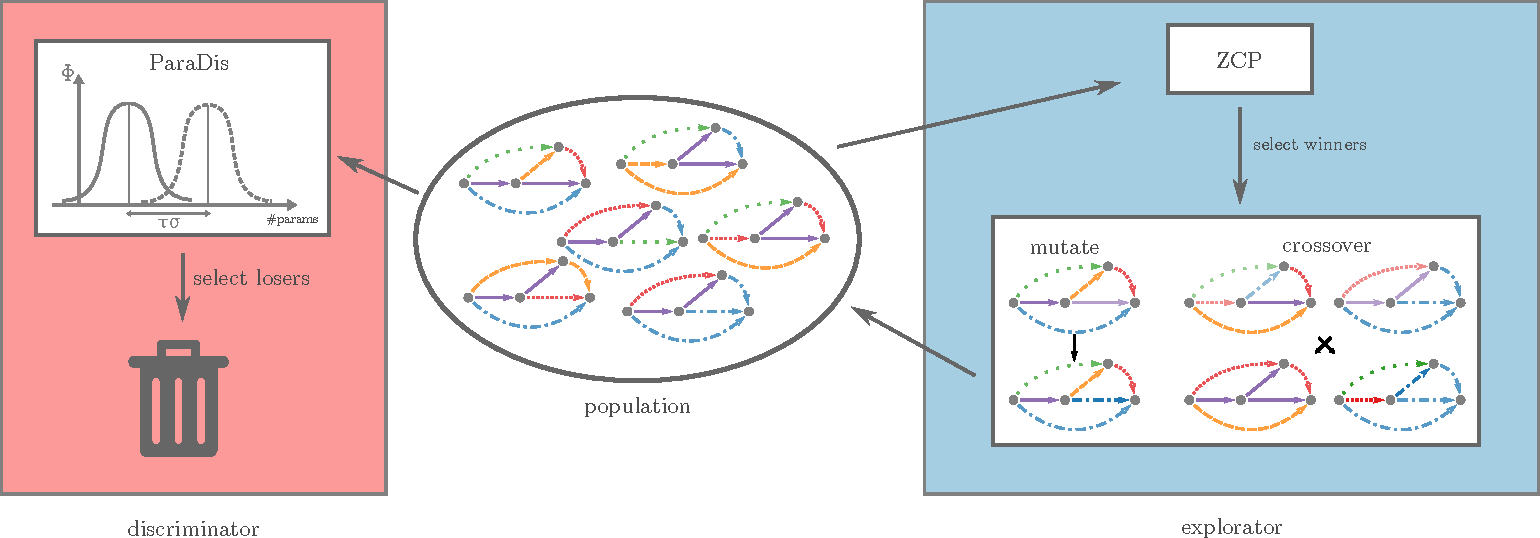
\includegraphics[width=\textwidth]{fig/paradis.pdf}

\end{adjustbox}
\caption{Our ParaDis method is based on the classic genetic zero-cost framework. Any ZCP can be used in the role of the explorer and select architectures that go on to reproduction. The ParaDis discriminator discards architectures based on parameter count distribution statistics over the population, with the size of architectures sampled at each generation controlled by $\tau$.
}
\label{fig_main_method}
\end{figure}

\section{Related works}
\label{related}

\paragraph{Zero-cost proxies} Zero-cost proxies (ZCPs) \citep{mellor2021neural, abdelfattah2021zero} hold the potential to conduct neural architecture search without the need to train architectures. ZCPs are generally derived from mathematical properties of neural networks computed from their parameters or gradients, which can be obtained during a single forward or backward pass. While most ZCPs rely on actual data from the task, metrics such as \texttt{synflow} operate in a data-agnostic regime, and quantifiable properties of the networks such as parameter count (\texttt{\#params}) can also be considered data-agnostic ZCPs. Compared to data-reliant ZCPs, data agnosticity yields better robustness when confronted with diverse tasks, and ease of implementation as a data loading pipeline is not required.

Various ZCPs have been introduced for the purpose of architecture search. Initially, \citet{mellor2021neural} proposed to use the Hamming distance of the binary codes of the activations, a proxy which was later renamed \texttt{jacov}.~\citet{abdelfattah2021zero} brought metrics from the network pruning literature into the NAS space and coined the term ZCP. ZCPs tend to fall into two categories based on whether they aim to quantify the trainability of the candidate --- that is, how easily it can converge to its optimal weights --- or its generalization capabilities. Thus, the metrics \texttt{gradnorm}, \texttt{snip}, \texttt{grasp} and \texttt{synflow} are of the trainability type, while \texttt{fisher} is of the generalization type. This observation was further explored in \citet{chen2021neural}, who paired the trainability measure \texttt{ntk}, based on the NTK condition number \citep{xiao2019disentangling}, and the expressivity measure \texttt{\#lr}, a count of the number of linear regions of the input space partitioned by the network \citep{raghu2017expressive}.

Recently, more advanced ZCPs have emerged and demonstrated competitive results on vision tasks. \texttt{zen} \citep{lin2021zen} leverages the statistics of the batch norm layers. \texttt{zico} \citep{li2023zico} exploits the link between the statistics of the gradient norms and network generalization ability. \texttt{meco} \citep{jiang2023meco} estimates the convergence rate via the minimum eigenvalue of the correlation matrix. \texttt{swap} \citep{peng2024swap} reframes the question of linear regions to create a more insightful metric.

\paragraph{Zero-shot NAS} Since ZCPs are essentially performance estimators, they must be paired with a search strategy to explore the search space. Several possibilities have been explored in previous work. \citet{mellor2021neural} proposed the naive random search solution, and warm-started other traditional NAS methods with the ZCP. Similarly, \citet{abdelfattah2021zero} envisioned ZCPs as a warmup for other algorithms. \citet{chen2021neural} and \citet{jiang2023meco} implemented a pruning-like strategy where a directed acyclic graph containing all possible architectural choices is pruned down to only the most desirable operation on each edge. 

However, the most popular search strategy in conjunction with ZCPs remains by far the genetic approach \citep{lin2021zen, li2023zico, peng2024swap}. It is also a very common strategy for NAS in general \citep{real2018regularized, ericsson2024einspace}. In this work, we also adopt the evolutionary framework. While other NAS methods keep the algorithmic design to a bare minimum, choosing to instead focus on the proxies' capabilities, we directly improve on the classic genetic algorithm to cover the limits of ZCPs. Importantly, this allows us to remain orthogonal to ZCP design.

\paragraph{ZCP ensembling} Intuitively, using more than one proxy should be beneficial, since metrics that evaluate different aspects of a network might cover each other's blind spots.~\citet{chen2021neural} first introduced this idea by summing their \texttt{ntk} and \texttt{\#lr} metrics. \citet{he2024robustifying} generalized the idea by ensembling 6 ZCPs through weighted linear combination and learning the weights through Bayesian optimization. However, direct summation of ZCPs is impractical as the statistics of individual proxies are task-dependent and largely unknown. Without robust normalization, such sums are highly sensitive to outliers.~\citet{kadlecova2024surprisingly} instead ensemble proxies by treating them as features of the candidate architectures and applying random forest regression. Differently, we assign roles to ZCPs within the genetic framework such that they guide exploration of the search space or discriminate architectures to constrain the space.

\paragraph{Parameter count} Simply counting the parameters of a candidate architecture is a naive, yet effective proxy for accuracy. Indeed, network complexity and generalization abilities grow with network size. Notably, the surprising effectiveness of the parameter count proxy \texttt{\#params} often challenges ZCPs \citep{colin2022adeeperlook, javaheripi2022litetransformersearch}, which are shown to be inferior to merely counting the parameters on various tasks. While this metric lacks the nuance to discern common architectural choices such as skip connections, a staple of architecture design shown to improve trainability \citep{he2015deep, orhan2017skip}, complex ZCPs might identify these intricacies while failing to describe the bigger picture.

We propose that the parameter count may serve as a prerequisite metric and adopt it as a regularizer of the search.~\citet{peng2024swap} also used parameter count to regularize the score of their metric \texttt{swap} and focus the search around a desired model size. However, this requires prior knowledge of the search space's statistics, which is impractical for unseen spaces where the location of good architectures in the distribution is unknown. We instead design our method in a space-agnostic way by estimating parameter count statistics directly from available sampled architectures, removing the need for priors over the space. This allows the method to continue performing in real-world spaces with unknown structures.

\begin{figure}[t]
\begin{adjustbox}{width=\linewidth}
    %% Creator: Matplotlib, PGF backend
%%
%% To include the figure in your LaTeX document, write
%%   \input{<filename>.pgf}
%%
%% Make sure the required packages are loaded in your preamble
%%   \usepackage{pgf}
%%
%% Also ensure that all the required font packages are loaded; for instance,
%% the lmodern package is sometimes necessary when using math font.
%%   \usepackage{lmodern}
%%
%% Figures using additional raster images can only be included by \input if
%% they are in the same directory as the main LaTeX file. For loading figures
%% from other directories you can use the `import` package
%%   \usepackage{import}
%%
%% and then include the figures with
%%   \import{<path to file>}{<filename>.pgf}
%%
%% Matplotlib used the following preamble
%%   
%%   \usepackage{fontspec}
%%   \setmainfont{DejaVuSerif.ttf}[Path=\detokenize{/home/t19lyman/.local/lib/python3.10/site-packages/matplotlib/mpl-data/fonts/ttf/}]
%%   \setsansfont{arial.ttf}[Path=\detokenize{/usr/share/fonts/WindowsFonts/Fonts/}]
%%   \setmonofont{DejaVuSansMono.ttf}[Path=\detokenize{/home/t19lyman/.local/lib/python3.10/site-packages/matplotlib/mpl-data/fonts/ttf/}]
%%   \makeatletter\@ifpackageloaded{underscore}{}{\usepackage[strings]{underscore}}\makeatother
%%
\begingroup%
\makeatletter%
\begin{pgfpicture}%
\pgfpathrectangle{\pgfpointorigin}{\pgfqpoint{8.894522in}{3.888489in}}%
\pgfusepath{use as bounding box, clip}%
\begin{pgfscope}%
\pgfsetbuttcap%
\pgfsetmiterjoin%
\definecolor{currentfill}{rgb}{1.000000,1.000000,1.000000}%
\pgfsetfillcolor{currentfill}%
\pgfsetlinewidth{0.000000pt}%
\definecolor{currentstroke}{rgb}{1.000000,1.000000,1.000000}%
\pgfsetstrokecolor{currentstroke}%
\pgfsetdash{}{0pt}%
\pgfpathmoveto{\pgfqpoint{0.000000in}{0.000000in}}%
\pgfpathlineto{\pgfqpoint{8.894522in}{0.000000in}}%
\pgfpathlineto{\pgfqpoint{8.894522in}{3.888489in}}%
\pgfpathlineto{\pgfqpoint{0.000000in}{3.888489in}}%
\pgfpathlineto{\pgfqpoint{0.000000in}{0.000000in}}%
\pgfpathclose%
\pgfusepath{fill}%
\end{pgfscope}%
\begin{pgfscope}%
\pgfsetbuttcap%
\pgfsetmiterjoin%
\definecolor{currentfill}{rgb}{0.917647,0.917647,0.949020}%
\pgfsetfillcolor{currentfill}%
\pgfsetlinewidth{0.000000pt}%
\definecolor{currentstroke}{rgb}{0.000000,0.000000,0.000000}%
\pgfsetstrokecolor{currentstroke}%
\pgfsetstrokeopacity{0.000000}%
\pgfsetdash{}{0pt}%
\pgfpathmoveto{\pgfqpoint{0.935592in}{1.185177in}}%
\pgfpathlineto{\pgfqpoint{8.794522in}{1.185177in}}%
\pgfpathlineto{\pgfqpoint{8.794522in}{3.788489in}}%
\pgfpathlineto{\pgfqpoint{0.935592in}{3.788489in}}%
\pgfpathlineto{\pgfqpoint{0.935592in}{1.185177in}}%
\pgfpathclose%
\pgfusepath{fill}%
\end{pgfscope}%
\begin{pgfscope}%
\pgfpathrectangle{\pgfqpoint{0.935592in}{1.185177in}}{\pgfqpoint{7.858931in}{2.603312in}}%
\pgfusepath{clip}%
\pgfsetroundcap%
\pgfsetroundjoin%
\pgfsetlinewidth{1.003750pt}%
\definecolor{currentstroke}{rgb}{1.000000,1.000000,1.000000}%
\pgfsetstrokecolor{currentstroke}%
\pgfsetdash{}{0pt}%
\pgfpathmoveto{\pgfqpoint{1.153895in}{1.185177in}}%
\pgfpathlineto{\pgfqpoint{1.153895in}{3.788489in}}%
\pgfusepath{stroke}%
\end{pgfscope}%
\begin{pgfscope}%
\definecolor{textcolor}{rgb}{0.150000,0.150000,0.150000}%
\pgfsetstrokecolor{textcolor}%
\pgfsetfillcolor{textcolor}%
\pgftext[x=0.415296in, y=0.543110in, left, base,rotate=30.000000]{\color{textcolor}\ttfamily\fontsize{10.000000}{12.000000}\selectfont NB201-CF10}%
\end{pgfscope}%
\begin{pgfscope}%
\pgfpathrectangle{\pgfqpoint{0.935592in}{1.185177in}}{\pgfqpoint{7.858931in}{2.603312in}}%
\pgfusepath{clip}%
\pgfsetroundcap%
\pgfsetroundjoin%
\pgfsetlinewidth{1.003750pt}%
\definecolor{currentstroke}{rgb}{1.000000,1.000000,1.000000}%
\pgfsetstrokecolor{currentstroke}%
\pgfsetdash{}{0pt}%
\pgfpathmoveto{\pgfqpoint{1.590503in}{1.185177in}}%
\pgfpathlineto{\pgfqpoint{1.590503in}{3.788489in}}%
\pgfusepath{stroke}%
\end{pgfscope}%
\begin{pgfscope}%
\definecolor{textcolor}{rgb}{0.150000,0.150000,0.150000}%
\pgfsetstrokecolor{textcolor}%
\pgfsetfillcolor{textcolor}%
\pgftext[x=0.779488in, y=0.501301in, left, base,rotate=30.000000]{\color{textcolor}\ttfamily\fontsize{10.000000}{12.000000}\selectfont NB201-CF100}%
\end{pgfscope}%
\begin{pgfscope}%
\pgfpathrectangle{\pgfqpoint{0.935592in}{1.185177in}}{\pgfqpoint{7.858931in}{2.603312in}}%
\pgfusepath{clip}%
\pgfsetroundcap%
\pgfsetroundjoin%
\pgfsetlinewidth{1.003750pt}%
\definecolor{currentstroke}{rgb}{1.000000,1.000000,1.000000}%
\pgfsetstrokecolor{currentstroke}%
\pgfsetdash{}{0pt}%
\pgfpathmoveto{\pgfqpoint{2.027110in}{1.185177in}}%
\pgfpathlineto{\pgfqpoint{2.027110in}{3.788489in}}%
\pgfusepath{stroke}%
\end{pgfscope}%
\begin{pgfscope}%
\definecolor{textcolor}{rgb}{0.150000,0.150000,0.150000}%
\pgfsetstrokecolor{textcolor}%
\pgfsetfillcolor{textcolor}%
\pgftext[x=1.216095in, y=0.501301in, left, base,rotate=30.000000]{\color{textcolor}\ttfamily\fontsize{10.000000}{12.000000}\selectfont NB201-IMGNT}%
\end{pgfscope}%
\begin{pgfscope}%
\pgfpathrectangle{\pgfqpoint{0.935592in}{1.185177in}}{\pgfqpoint{7.858931in}{2.603312in}}%
\pgfusepath{clip}%
\pgfsetroundcap%
\pgfsetroundjoin%
\pgfsetlinewidth{1.003750pt}%
\definecolor{currentstroke}{rgb}{1.000000,1.000000,1.000000}%
\pgfsetstrokecolor{currentstroke}%
\pgfsetdash{}{0pt}%
\pgfpathmoveto{\pgfqpoint{2.463717in}{1.185177in}}%
\pgfpathlineto{\pgfqpoint{2.463717in}{3.788489in}}%
\pgfusepath{stroke}%
\end{pgfscope}%
\begin{pgfscope}%
\definecolor{textcolor}{rgb}{0.150000,0.150000,0.150000}%
\pgfsetstrokecolor{textcolor}%
\pgfsetfillcolor{textcolor}%
\pgftext[x=1.725118in, y=0.543110in, left, base,rotate=30.000000]{\color{textcolor}\ttfamily\fontsize{10.000000}{12.000000}\selectfont NB301-CF10}%
\end{pgfscope}%
\begin{pgfscope}%
\pgfpathrectangle{\pgfqpoint{0.935592in}{1.185177in}}{\pgfqpoint{7.858931in}{2.603312in}}%
\pgfusepath{clip}%
\pgfsetroundcap%
\pgfsetroundjoin%
\pgfsetlinewidth{1.003750pt}%
\definecolor{currentstroke}{rgb}{1.000000,1.000000,1.000000}%
\pgfsetstrokecolor{currentstroke}%
\pgfsetdash{}{0pt}%
\pgfpathmoveto{\pgfqpoint{2.900324in}{1.185177in}}%
\pgfpathlineto{\pgfqpoint{2.900324in}{3.788489in}}%
\pgfusepath{stroke}%
\end{pgfscope}%
\begin{pgfscope}%
\definecolor{textcolor}{rgb}{0.150000,0.150000,0.150000}%
\pgfsetstrokecolor{textcolor}%
\pgfsetfillcolor{textcolor}%
\pgftext[x=1.509986in, y=0.166828in, left, base,rotate=30.000000]{\color{textcolor}\ttfamily\fontsize{10.000000}{12.000000}\selectfont TNB101-MICRO-JIGSAW}%
\end{pgfscope}%
\begin{pgfscope}%
\pgfpathrectangle{\pgfqpoint{0.935592in}{1.185177in}}{\pgfqpoint{7.858931in}{2.603312in}}%
\pgfusepath{clip}%
\pgfsetroundcap%
\pgfsetroundjoin%
\pgfsetlinewidth{1.003750pt}%
\definecolor{currentstroke}{rgb}{1.000000,1.000000,1.000000}%
\pgfsetstrokecolor{currentstroke}%
\pgfsetdash{}{0pt}%
\pgfpathmoveto{\pgfqpoint{3.336932in}{1.185177in}}%
\pgfpathlineto{\pgfqpoint{3.336932in}{3.788489in}}%
\pgfusepath{stroke}%
\end{pgfscope}%
\begin{pgfscope}%
\definecolor{textcolor}{rgb}{0.150000,0.150000,0.150000}%
\pgfsetstrokecolor{textcolor}%
\pgfsetfillcolor{textcolor}%
\pgftext[x=2.019009in, y=0.208637in, left, base,rotate=30.000000]{\color{textcolor}\ttfamily\fontsize{10.000000}{12.000000}\selectfont TNB101-MICRO-SCENE}%
\end{pgfscope}%
\begin{pgfscope}%
\pgfpathrectangle{\pgfqpoint{0.935592in}{1.185177in}}{\pgfqpoint{7.858931in}{2.603312in}}%
\pgfusepath{clip}%
\pgfsetroundcap%
\pgfsetroundjoin%
\pgfsetlinewidth{1.003750pt}%
\definecolor{currentstroke}{rgb}{1.000000,1.000000,1.000000}%
\pgfsetstrokecolor{currentstroke}%
\pgfsetdash{}{0pt}%
\pgfpathmoveto{\pgfqpoint{3.773539in}{1.185177in}}%
\pgfpathlineto{\pgfqpoint{3.773539in}{3.788489in}}%
\pgfusepath{stroke}%
\end{pgfscope}%
\begin{pgfscope}%
\definecolor{textcolor}{rgb}{0.150000,0.150000,0.150000}%
\pgfsetstrokecolor{textcolor}%
\pgfsetfillcolor{textcolor}%
\pgftext[x=2.383200in, y=0.166828in, left, base,rotate=30.000000]{\color{textcolor}\ttfamily\fontsize{10.000000}{12.000000}\selectfont TNB101-MICRO-OBJECT}%
\end{pgfscope}%
\begin{pgfscope}%
\pgfpathrectangle{\pgfqpoint{0.935592in}{1.185177in}}{\pgfqpoint{7.858931in}{2.603312in}}%
\pgfusepath{clip}%
\pgfsetroundcap%
\pgfsetroundjoin%
\pgfsetlinewidth{1.003750pt}%
\definecolor{currentstroke}{rgb}{1.000000,1.000000,1.000000}%
\pgfsetstrokecolor{currentstroke}%
\pgfsetdash{}{0pt}%
\pgfpathmoveto{\pgfqpoint{4.210146in}{1.185177in}}%
\pgfpathlineto{\pgfqpoint{4.210146in}{3.788489in}}%
\pgfusepath{stroke}%
\end{pgfscope}%
\begin{pgfscope}%
\definecolor{textcolor}{rgb}{0.150000,0.150000,0.150000}%
\pgfsetstrokecolor{textcolor}%
\pgfsetfillcolor{textcolor}%
\pgftext[x=2.747392in, y=0.125019in, left, base,rotate=30.000000]{\color{textcolor}\ttfamily\fontsize{10.000000}{12.000000}\selectfont TNB101-MICRO-AUTOENC}%
\end{pgfscope}%
\begin{pgfscope}%
\pgfpathrectangle{\pgfqpoint{0.935592in}{1.185177in}}{\pgfqpoint{7.858931in}{2.603312in}}%
\pgfusepath{clip}%
\pgfsetroundcap%
\pgfsetroundjoin%
\pgfsetlinewidth{1.003750pt}%
\definecolor{currentstroke}{rgb}{1.000000,1.000000,1.000000}%
\pgfsetstrokecolor{currentstroke}%
\pgfsetdash{}{0pt}%
\pgfpathmoveto{\pgfqpoint{4.646753in}{1.185177in}}%
\pgfpathlineto{\pgfqpoint{4.646753in}{3.788489in}}%
\pgfusepath{stroke}%
\end{pgfscope}%
\begin{pgfscope}%
\definecolor{textcolor}{rgb}{0.150000,0.150000,0.150000}%
\pgfsetstrokecolor{textcolor}%
\pgfsetfillcolor{textcolor}%
\pgftext[x=3.256415in, y=0.166828in, left, base,rotate=30.000000]{\color{textcolor}\ttfamily\fontsize{10.000000}{12.000000}\selectfont TNB101-MICRO-NORMAL}%
\end{pgfscope}%
\begin{pgfscope}%
\pgfpathrectangle{\pgfqpoint{0.935592in}{1.185177in}}{\pgfqpoint{7.858931in}{2.603312in}}%
\pgfusepath{clip}%
\pgfsetroundcap%
\pgfsetroundjoin%
\pgfsetlinewidth{1.003750pt}%
\definecolor{currentstroke}{rgb}{1.000000,1.000000,1.000000}%
\pgfsetstrokecolor{currentstroke}%
\pgfsetdash{}{0pt}%
\pgfpathmoveto{\pgfqpoint{5.083361in}{1.185177in}}%
\pgfpathlineto{\pgfqpoint{5.083361in}{3.788489in}}%
\pgfusepath{stroke}%
\end{pgfscope}%
\begin{pgfscope}%
\definecolor{textcolor}{rgb}{0.150000,0.150000,0.150000}%
\pgfsetstrokecolor{textcolor}%
\pgfsetfillcolor{textcolor}%
\pgftext[x=3.837853in, y=0.250447in, left, base,rotate=30.000000]{\color{textcolor}\ttfamily\fontsize{10.000000}{12.000000}\selectfont TNB101-MICRO-ROOM}%
\end{pgfscope}%
\begin{pgfscope}%
\pgfpathrectangle{\pgfqpoint{0.935592in}{1.185177in}}{\pgfqpoint{7.858931in}{2.603312in}}%
\pgfusepath{clip}%
\pgfsetroundcap%
\pgfsetroundjoin%
\pgfsetlinewidth{1.003750pt}%
\definecolor{currentstroke}{rgb}{1.000000,1.000000,1.000000}%
\pgfsetstrokecolor{currentstroke}%
\pgfsetdash{}{0pt}%
\pgfpathmoveto{\pgfqpoint{5.519968in}{1.185177in}}%
\pgfpathlineto{\pgfqpoint{5.519968in}{3.788489in}}%
\pgfusepath{stroke}%
\end{pgfscope}%
\begin{pgfscope}%
\definecolor{textcolor}{rgb}{0.150000,0.150000,0.150000}%
\pgfsetstrokecolor{textcolor}%
\pgfsetfillcolor{textcolor}%
\pgftext[x=4.057214in, y=0.125019in, left, base,rotate=30.000000]{\color{textcolor}\ttfamily\fontsize{10.000000}{12.000000}\selectfont TNB101-MICRO-SEGMENT}%
\end{pgfscope}%
\begin{pgfscope}%
\pgfpathrectangle{\pgfqpoint{0.935592in}{1.185177in}}{\pgfqpoint{7.858931in}{2.603312in}}%
\pgfusepath{clip}%
\pgfsetroundcap%
\pgfsetroundjoin%
\pgfsetlinewidth{1.003750pt}%
\definecolor{currentstroke}{rgb}{1.000000,1.000000,1.000000}%
\pgfsetstrokecolor{currentstroke}%
\pgfsetdash{}{0pt}%
\pgfpathmoveto{\pgfqpoint{5.956575in}{1.185177in}}%
\pgfpathlineto{\pgfqpoint{5.956575in}{3.788489in}}%
\pgfusepath{stroke}%
\end{pgfscope}%
\begin{pgfscope}%
\definecolor{textcolor}{rgb}{0.150000,0.150000,0.150000}%
\pgfsetstrokecolor{textcolor}%
\pgfsetfillcolor{textcolor}%
\pgftext[x=4.566237in, y=0.166828in, left, base,rotate=30.000000]{\color{textcolor}\ttfamily\fontsize{10.000000}{12.000000}\selectfont TNB101-MACRO-JIGSAW}%
\end{pgfscope}%
\begin{pgfscope}%
\pgfpathrectangle{\pgfqpoint{0.935592in}{1.185177in}}{\pgfqpoint{7.858931in}{2.603312in}}%
\pgfusepath{clip}%
\pgfsetroundcap%
\pgfsetroundjoin%
\pgfsetlinewidth{1.003750pt}%
\definecolor{currentstroke}{rgb}{1.000000,1.000000,1.000000}%
\pgfsetstrokecolor{currentstroke}%
\pgfsetdash{}{0pt}%
\pgfpathmoveto{\pgfqpoint{6.393182in}{1.185177in}}%
\pgfpathlineto{\pgfqpoint{6.393182in}{3.788489in}}%
\pgfusepath{stroke}%
\end{pgfscope}%
\begin{pgfscope}%
\definecolor{textcolor}{rgb}{0.150000,0.150000,0.150000}%
\pgfsetstrokecolor{textcolor}%
\pgfsetfillcolor{textcolor}%
\pgftext[x=5.075259in, y=0.208637in, left, base,rotate=30.000000]{\color{textcolor}\ttfamily\fontsize{10.000000}{12.000000}\selectfont TNB101-MACRO-SCENE}%
\end{pgfscope}%
\begin{pgfscope}%
\pgfpathrectangle{\pgfqpoint{0.935592in}{1.185177in}}{\pgfqpoint{7.858931in}{2.603312in}}%
\pgfusepath{clip}%
\pgfsetroundcap%
\pgfsetroundjoin%
\pgfsetlinewidth{1.003750pt}%
\definecolor{currentstroke}{rgb}{1.000000,1.000000,1.000000}%
\pgfsetstrokecolor{currentstroke}%
\pgfsetdash{}{0pt}%
\pgfpathmoveto{\pgfqpoint{6.829790in}{1.185177in}}%
\pgfpathlineto{\pgfqpoint{6.829790in}{3.788489in}}%
\pgfusepath{stroke}%
\end{pgfscope}%
\begin{pgfscope}%
\definecolor{textcolor}{rgb}{0.150000,0.150000,0.150000}%
\pgfsetstrokecolor{textcolor}%
\pgfsetfillcolor{textcolor}%
\pgftext[x=5.439451in, y=0.166828in, left, base,rotate=30.000000]{\color{textcolor}\ttfamily\fontsize{10.000000}{12.000000}\selectfont TNB101-MACRO-OBJECT}%
\end{pgfscope}%
\begin{pgfscope}%
\pgfpathrectangle{\pgfqpoint{0.935592in}{1.185177in}}{\pgfqpoint{7.858931in}{2.603312in}}%
\pgfusepath{clip}%
\pgfsetroundcap%
\pgfsetroundjoin%
\pgfsetlinewidth{1.003750pt}%
\definecolor{currentstroke}{rgb}{1.000000,1.000000,1.000000}%
\pgfsetstrokecolor{currentstroke}%
\pgfsetdash{}{0pt}%
\pgfpathmoveto{\pgfqpoint{7.266397in}{1.185177in}}%
\pgfpathlineto{\pgfqpoint{7.266397in}{3.788489in}}%
\pgfusepath{stroke}%
\end{pgfscope}%
\begin{pgfscope}%
\definecolor{textcolor}{rgb}{0.150000,0.150000,0.150000}%
\pgfsetstrokecolor{textcolor}%
\pgfsetfillcolor{textcolor}%
\pgftext[x=5.803643in, y=0.125019in, left, base,rotate=30.000000]{\color{textcolor}\ttfamily\fontsize{10.000000}{12.000000}\selectfont TNB101-MACRO-AUTOENC}%
\end{pgfscope}%
\begin{pgfscope}%
\pgfpathrectangle{\pgfqpoint{0.935592in}{1.185177in}}{\pgfqpoint{7.858931in}{2.603312in}}%
\pgfusepath{clip}%
\pgfsetroundcap%
\pgfsetroundjoin%
\pgfsetlinewidth{1.003750pt}%
\definecolor{currentstroke}{rgb}{1.000000,1.000000,1.000000}%
\pgfsetstrokecolor{currentstroke}%
\pgfsetdash{}{0pt}%
\pgfpathmoveto{\pgfqpoint{7.703004in}{1.185177in}}%
\pgfpathlineto{\pgfqpoint{7.703004in}{3.788489in}}%
\pgfusepath{stroke}%
\end{pgfscope}%
\begin{pgfscope}%
\definecolor{textcolor}{rgb}{0.150000,0.150000,0.150000}%
\pgfsetstrokecolor{textcolor}%
\pgfsetfillcolor{textcolor}%
\pgftext[x=6.312666in, y=0.166828in, left, base,rotate=30.000000]{\color{textcolor}\ttfamily\fontsize{10.000000}{12.000000}\selectfont TNB101-MACRO-NORMAL}%
\end{pgfscope}%
\begin{pgfscope}%
\pgfpathrectangle{\pgfqpoint{0.935592in}{1.185177in}}{\pgfqpoint{7.858931in}{2.603312in}}%
\pgfusepath{clip}%
\pgfsetroundcap%
\pgfsetroundjoin%
\pgfsetlinewidth{1.003750pt}%
\definecolor{currentstroke}{rgb}{1.000000,1.000000,1.000000}%
\pgfsetstrokecolor{currentstroke}%
\pgfsetdash{}{0pt}%
\pgfpathmoveto{\pgfqpoint{8.139611in}{1.185177in}}%
\pgfpathlineto{\pgfqpoint{8.139611in}{3.788489in}}%
\pgfusepath{stroke}%
\end{pgfscope}%
\begin{pgfscope}%
\definecolor{textcolor}{rgb}{0.150000,0.150000,0.150000}%
\pgfsetstrokecolor{textcolor}%
\pgfsetfillcolor{textcolor}%
\pgftext[x=6.894104in, y=0.250447in, left, base,rotate=30.000000]{\color{textcolor}\ttfamily\fontsize{10.000000}{12.000000}\selectfont TNB101-MACRO-ROOM}%
\end{pgfscope}%
\begin{pgfscope}%
\pgfpathrectangle{\pgfqpoint{0.935592in}{1.185177in}}{\pgfqpoint{7.858931in}{2.603312in}}%
\pgfusepath{clip}%
\pgfsetroundcap%
\pgfsetroundjoin%
\pgfsetlinewidth{1.003750pt}%
\definecolor{currentstroke}{rgb}{1.000000,1.000000,1.000000}%
\pgfsetstrokecolor{currentstroke}%
\pgfsetdash{}{0pt}%
\pgfpathmoveto{\pgfqpoint{8.576219in}{1.185177in}}%
\pgfpathlineto{\pgfqpoint{8.576219in}{3.788489in}}%
\pgfusepath{stroke}%
\end{pgfscope}%
\begin{pgfscope}%
\definecolor{textcolor}{rgb}{0.150000,0.150000,0.150000}%
\pgfsetstrokecolor{textcolor}%
\pgfsetfillcolor{textcolor}%
\pgftext[x=7.113465in, y=0.125019in, left, base,rotate=30.000000]{\color{textcolor}\ttfamily\fontsize{10.000000}{12.000000}\selectfont TNB101-MACRO-SEGMENT}%
\end{pgfscope}%
\begin{pgfscope}%
\pgfpathrectangle{\pgfqpoint{0.935592in}{1.185177in}}{\pgfqpoint{7.858931in}{2.603312in}}%
\pgfusepath{clip}%
\pgfsetroundcap%
\pgfsetroundjoin%
\pgfsetlinewidth{1.003750pt}%
\definecolor{currentstroke}{rgb}{1.000000,1.000000,1.000000}%
\pgfsetstrokecolor{currentstroke}%
\pgfsetdash{}{0pt}%
\pgfpathmoveto{\pgfqpoint{0.935592in}{3.680018in}}%
\pgfpathlineto{\pgfqpoint{8.794522in}{3.680018in}}%
\pgfusepath{stroke}%
\end{pgfscope}%
\begin{pgfscope}%
\definecolor{textcolor}{rgb}{0.150000,0.150000,0.150000}%
\pgfsetstrokecolor{textcolor}%
\pgfsetfillcolor{textcolor}%
\pgftext[x=0.803647in,y=3.680018in,right,]{\color{textcolor}\ttfamily\fontsize{9.350000}{11.220000}\selectfont params}%
\end{pgfscope}%
\begin{pgfscope}%
\pgfpathrectangle{\pgfqpoint{0.935592in}{1.185177in}}{\pgfqpoint{7.858931in}{2.603312in}}%
\pgfusepath{clip}%
\pgfsetroundcap%
\pgfsetroundjoin%
\pgfsetlinewidth{1.003750pt}%
\definecolor{currentstroke}{rgb}{1.000000,1.000000,1.000000}%
\pgfsetstrokecolor{currentstroke}%
\pgfsetdash{}{0pt}%
\pgfpathmoveto{\pgfqpoint{0.935592in}{3.463075in}}%
\pgfpathlineto{\pgfqpoint{8.794522in}{3.463075in}}%
\pgfusepath{stroke}%
\end{pgfscope}%
\begin{pgfscope}%
\definecolor{textcolor}{rgb}{0.150000,0.150000,0.150000}%
\pgfsetstrokecolor{textcolor}%
\pgfsetfillcolor{textcolor}%
\pgftext[x=0.803647in,y=3.463075in,right,]{\color{textcolor}\ttfamily\fontsize{9.350000}{11.220000}\selectfont grad\_norm}%
\end{pgfscope}%
\begin{pgfscope}%
\pgfpathrectangle{\pgfqpoint{0.935592in}{1.185177in}}{\pgfqpoint{7.858931in}{2.603312in}}%
\pgfusepath{clip}%
\pgfsetroundcap%
\pgfsetroundjoin%
\pgfsetlinewidth{1.003750pt}%
\definecolor{currentstroke}{rgb}{1.000000,1.000000,1.000000}%
\pgfsetstrokecolor{currentstroke}%
\pgfsetdash{}{0pt}%
\pgfpathmoveto{\pgfqpoint{0.935592in}{3.246132in}}%
\pgfpathlineto{\pgfqpoint{8.794522in}{3.246132in}}%
\pgfusepath{stroke}%
\end{pgfscope}%
\begin{pgfscope}%
\definecolor{textcolor}{rgb}{0.150000,0.150000,0.150000}%
\pgfsetstrokecolor{textcolor}%
\pgfsetfillcolor{textcolor}%
\pgftext[x=0.803647in,y=3.246132in,right,]{\color{textcolor}\ttfamily\fontsize{9.350000}{11.220000}\selectfont fisher}%
\end{pgfscope}%
\begin{pgfscope}%
\pgfpathrectangle{\pgfqpoint{0.935592in}{1.185177in}}{\pgfqpoint{7.858931in}{2.603312in}}%
\pgfusepath{clip}%
\pgfsetroundcap%
\pgfsetroundjoin%
\pgfsetlinewidth{1.003750pt}%
\definecolor{currentstroke}{rgb}{1.000000,1.000000,1.000000}%
\pgfsetstrokecolor{currentstroke}%
\pgfsetdash{}{0pt}%
\pgfpathmoveto{\pgfqpoint{0.935592in}{3.029190in}}%
\pgfpathlineto{\pgfqpoint{8.794522in}{3.029190in}}%
\pgfusepath{stroke}%
\end{pgfscope}%
\begin{pgfscope}%
\definecolor{textcolor}{rgb}{0.150000,0.150000,0.150000}%
\pgfsetstrokecolor{textcolor}%
\pgfsetfillcolor{textcolor}%
\pgftext[x=0.803647in,y=3.029190in,right,]{\color{textcolor}\ttfamily\fontsize{9.350000}{11.220000}\selectfont jacov}%
\end{pgfscope}%
\begin{pgfscope}%
\pgfpathrectangle{\pgfqpoint{0.935592in}{1.185177in}}{\pgfqpoint{7.858931in}{2.603312in}}%
\pgfusepath{clip}%
\pgfsetroundcap%
\pgfsetroundjoin%
\pgfsetlinewidth{1.003750pt}%
\definecolor{currentstroke}{rgb}{1.000000,1.000000,1.000000}%
\pgfsetstrokecolor{currentstroke}%
\pgfsetdash{}{0pt}%
\pgfpathmoveto{\pgfqpoint{0.935592in}{2.812247in}}%
\pgfpathlineto{\pgfqpoint{8.794522in}{2.812247in}}%
\pgfusepath{stroke}%
\end{pgfscope}%
\begin{pgfscope}%
\definecolor{textcolor}{rgb}{0.150000,0.150000,0.150000}%
\pgfsetstrokecolor{textcolor}%
\pgfsetfillcolor{textcolor}%
\pgftext[x=0.803647in,y=2.812247in,right,]{\color{textcolor}\ttfamily\fontsize{9.350000}{11.220000}\selectfont snip}%
\end{pgfscope}%
\begin{pgfscope}%
\pgfpathrectangle{\pgfqpoint{0.935592in}{1.185177in}}{\pgfqpoint{7.858931in}{2.603312in}}%
\pgfusepath{clip}%
\pgfsetroundcap%
\pgfsetroundjoin%
\pgfsetlinewidth{1.003750pt}%
\definecolor{currentstroke}{rgb}{1.000000,1.000000,1.000000}%
\pgfsetstrokecolor{currentstroke}%
\pgfsetdash{}{0pt}%
\pgfpathmoveto{\pgfqpoint{0.935592in}{2.595304in}}%
\pgfpathlineto{\pgfqpoint{8.794522in}{2.595304in}}%
\pgfusepath{stroke}%
\end{pgfscope}%
\begin{pgfscope}%
\definecolor{textcolor}{rgb}{0.150000,0.150000,0.150000}%
\pgfsetstrokecolor{textcolor}%
\pgfsetfillcolor{textcolor}%
\pgftext[x=0.803647in,y=2.595304in,right,]{\color{textcolor}\ttfamily\fontsize{9.350000}{11.220000}\selectfont grasp}%
\end{pgfscope}%
\begin{pgfscope}%
\pgfpathrectangle{\pgfqpoint{0.935592in}{1.185177in}}{\pgfqpoint{7.858931in}{2.603312in}}%
\pgfusepath{clip}%
\pgfsetroundcap%
\pgfsetroundjoin%
\pgfsetlinewidth{1.003750pt}%
\definecolor{currentstroke}{rgb}{1.000000,1.000000,1.000000}%
\pgfsetstrokecolor{currentstroke}%
\pgfsetdash{}{0pt}%
\pgfpathmoveto{\pgfqpoint{0.935592in}{2.378362in}}%
\pgfpathlineto{\pgfqpoint{8.794522in}{2.378362in}}%
\pgfusepath{stroke}%
\end{pgfscope}%
\begin{pgfscope}%
\definecolor{textcolor}{rgb}{0.150000,0.150000,0.150000}%
\pgfsetstrokecolor{textcolor}%
\pgfsetfillcolor{textcolor}%
\pgftext[x=0.803647in,y=2.378362in,right,]{\color{textcolor}\ttfamily\fontsize{9.350000}{11.220000}\selectfont synflow}%
\end{pgfscope}%
\begin{pgfscope}%
\pgfpathrectangle{\pgfqpoint{0.935592in}{1.185177in}}{\pgfqpoint{7.858931in}{2.603312in}}%
\pgfusepath{clip}%
\pgfsetroundcap%
\pgfsetroundjoin%
\pgfsetlinewidth{1.003750pt}%
\definecolor{currentstroke}{rgb}{1.000000,1.000000,1.000000}%
\pgfsetstrokecolor{currentstroke}%
\pgfsetdash{}{0pt}%
\pgfpathmoveto{\pgfqpoint{0.935592in}{2.161419in}}%
\pgfpathlineto{\pgfqpoint{8.794522in}{2.161419in}}%
\pgfusepath{stroke}%
\end{pgfscope}%
\begin{pgfscope}%
\definecolor{textcolor}{rgb}{0.150000,0.150000,0.150000}%
\pgfsetstrokecolor{textcolor}%
\pgfsetfillcolor{textcolor}%
\pgftext[x=0.803647in,y=2.161419in,right,]{\color{textcolor}\ttfamily\fontsize{9.350000}{11.220000}\selectfont ntk}%
\end{pgfscope}%
\begin{pgfscope}%
\pgfpathrectangle{\pgfqpoint{0.935592in}{1.185177in}}{\pgfqpoint{7.858931in}{2.603312in}}%
\pgfusepath{clip}%
\pgfsetroundcap%
\pgfsetroundjoin%
\pgfsetlinewidth{1.003750pt}%
\definecolor{currentstroke}{rgb}{1.000000,1.000000,1.000000}%
\pgfsetstrokecolor{currentstroke}%
\pgfsetdash{}{0pt}%
\pgfpathmoveto{\pgfqpoint{0.935592in}{1.944476in}}%
\pgfpathlineto{\pgfqpoint{8.794522in}{1.944476in}}%
\pgfusepath{stroke}%
\end{pgfscope}%
\begin{pgfscope}%
\definecolor{textcolor}{rgb}{0.150000,0.150000,0.150000}%
\pgfsetstrokecolor{textcolor}%
\pgfsetfillcolor{textcolor}%
\pgftext[x=0.803647in,y=1.944476in,right,]{\color{textcolor}\ttfamily\fontsize{9.350000}{11.220000}\selectfont zen}%
\end{pgfscope}%
\begin{pgfscope}%
\pgfpathrectangle{\pgfqpoint{0.935592in}{1.185177in}}{\pgfqpoint{7.858931in}{2.603312in}}%
\pgfusepath{clip}%
\pgfsetroundcap%
\pgfsetroundjoin%
\pgfsetlinewidth{1.003750pt}%
\definecolor{currentstroke}{rgb}{1.000000,1.000000,1.000000}%
\pgfsetstrokecolor{currentstroke}%
\pgfsetdash{}{0pt}%
\pgfpathmoveto{\pgfqpoint{0.935592in}{1.727534in}}%
\pgfpathlineto{\pgfqpoint{8.794522in}{1.727534in}}%
\pgfusepath{stroke}%
\end{pgfscope}%
\begin{pgfscope}%
\definecolor{textcolor}{rgb}{0.150000,0.150000,0.150000}%
\pgfsetstrokecolor{textcolor}%
\pgfsetfillcolor{textcolor}%
\pgftext[x=0.803647in,y=1.727534in,right,]{\color{textcolor}\ttfamily\fontsize{9.350000}{11.220000}\selectfont zico}%
\end{pgfscope}%
\begin{pgfscope}%
\pgfpathrectangle{\pgfqpoint{0.935592in}{1.185177in}}{\pgfqpoint{7.858931in}{2.603312in}}%
\pgfusepath{clip}%
\pgfsetroundcap%
\pgfsetroundjoin%
\pgfsetlinewidth{1.003750pt}%
\definecolor{currentstroke}{rgb}{1.000000,1.000000,1.000000}%
\pgfsetstrokecolor{currentstroke}%
\pgfsetdash{}{0pt}%
\pgfpathmoveto{\pgfqpoint{0.935592in}{1.510591in}}%
\pgfpathlineto{\pgfqpoint{8.794522in}{1.510591in}}%
\pgfusepath{stroke}%
\end{pgfscope}%
\begin{pgfscope}%
\definecolor{textcolor}{rgb}{0.150000,0.150000,0.150000}%
\pgfsetstrokecolor{textcolor}%
\pgfsetfillcolor{textcolor}%
\pgftext[x=0.803647in,y=1.510591in,right,]{\color{textcolor}\ttfamily\fontsize{9.350000}{11.220000}\selectfont meco}%
\end{pgfscope}%
\begin{pgfscope}%
\pgfpathrectangle{\pgfqpoint{0.935592in}{1.185177in}}{\pgfqpoint{7.858931in}{2.603312in}}%
\pgfusepath{clip}%
\pgfsetroundcap%
\pgfsetroundjoin%
\pgfsetlinewidth{1.003750pt}%
\definecolor{currentstroke}{rgb}{1.000000,1.000000,1.000000}%
\pgfsetstrokecolor{currentstroke}%
\pgfsetdash{}{0pt}%
\pgfpathmoveto{\pgfqpoint{0.935592in}{1.293648in}}%
\pgfpathlineto{\pgfqpoint{8.794522in}{1.293648in}}%
\pgfusepath{stroke}%
\end{pgfscope}%
\begin{pgfscope}%
\definecolor{textcolor}{rgb}{0.150000,0.150000,0.150000}%
\pgfsetstrokecolor{textcolor}%
\pgfsetfillcolor{textcolor}%
\pgftext[x=0.803647in,y=1.293648in,right,]{\color{textcolor}\ttfamily\fontsize{9.350000}{11.220000}\selectfont swap}%
\end{pgfscope}%
\begin{pgfscope}%
\pgfpathrectangle{\pgfqpoint{0.935592in}{1.185177in}}{\pgfqpoint{7.858931in}{2.603312in}}%
\pgfusepath{clip}%
\pgfsetbuttcap%
\pgfsetroundjoin%
\definecolor{currentfill}{rgb}{0.281412,0.155834,0.469201}%
\pgfsetfillcolor{currentfill}%
\pgfsetlinewidth{0.000000pt}%
\definecolor{currentstroke}{rgb}{1.000000,1.000000,1.000000}%
\pgfsetstrokecolor{currentstroke}%
\pgfsetdash{}{0pt}%
\pgfpathmoveto{\pgfqpoint{0.935592in}{3.788489in}}%
\pgfpathlineto{\pgfqpoint{1.372199in}{3.788489in}}%
\pgfpathlineto{\pgfqpoint{1.372199in}{3.571546in}}%
\pgfpathlineto{\pgfqpoint{0.935592in}{3.571546in}}%
\pgfpathlineto{\pgfqpoint{0.935592in}{3.788489in}}%
\pgfusepath{fill}%
\end{pgfscope}%
\begin{pgfscope}%
\pgfpathrectangle{\pgfqpoint{0.935592in}{1.185177in}}{\pgfqpoint{7.858931in}{2.603312in}}%
\pgfusepath{clip}%
\pgfsetbuttcap%
\pgfsetroundjoin%
\definecolor{currentfill}{rgb}{0.281412,0.155834,0.469201}%
\pgfsetfillcolor{currentfill}%
\pgfsetlinewidth{0.000000pt}%
\definecolor{currentstroke}{rgb}{1.000000,1.000000,1.000000}%
\pgfsetstrokecolor{currentstroke}%
\pgfsetdash{}{0pt}%
\pgfpathmoveto{\pgfqpoint{1.372199in}{3.788489in}}%
\pgfpathlineto{\pgfqpoint{1.808806in}{3.788489in}}%
\pgfpathlineto{\pgfqpoint{1.808806in}{3.571546in}}%
\pgfpathlineto{\pgfqpoint{1.372199in}{3.571546in}}%
\pgfpathlineto{\pgfqpoint{1.372199in}{3.788489in}}%
\pgfusepath{fill}%
\end{pgfscope}%
\begin{pgfscope}%
\pgfpathrectangle{\pgfqpoint{0.935592in}{1.185177in}}{\pgfqpoint{7.858931in}{2.603312in}}%
\pgfusepath{clip}%
\pgfsetbuttcap%
\pgfsetroundjoin%
\definecolor{currentfill}{rgb}{0.278012,0.180367,0.486697}%
\pgfsetfillcolor{currentfill}%
\pgfsetlinewidth{0.000000pt}%
\definecolor{currentstroke}{rgb}{1.000000,1.000000,1.000000}%
\pgfsetstrokecolor{currentstroke}%
\pgfsetdash{}{0pt}%
\pgfpathmoveto{\pgfqpoint{1.808806in}{3.788489in}}%
\pgfpathlineto{\pgfqpoint{2.245413in}{3.788489in}}%
\pgfpathlineto{\pgfqpoint{2.245413in}{3.571546in}}%
\pgfpathlineto{\pgfqpoint{1.808806in}{3.571546in}}%
\pgfpathlineto{\pgfqpoint{1.808806in}{3.788489in}}%
\pgfusepath{fill}%
\end{pgfscope}%
\begin{pgfscope}%
\pgfpathrectangle{\pgfqpoint{0.935592in}{1.185177in}}{\pgfqpoint{7.858931in}{2.603312in}}%
\pgfusepath{clip}%
\pgfsetbuttcap%
\pgfsetroundjoin%
\definecolor{currentfill}{rgb}{0.220057,0.343307,0.549413}%
\pgfsetfillcolor{currentfill}%
\pgfsetlinewidth{0.000000pt}%
\definecolor{currentstroke}{rgb}{1.000000,1.000000,1.000000}%
\pgfsetstrokecolor{currentstroke}%
\pgfsetdash{}{0pt}%
\pgfpathmoveto{\pgfqpoint{2.245413in}{3.788489in}}%
\pgfpathlineto{\pgfqpoint{2.682021in}{3.788489in}}%
\pgfpathlineto{\pgfqpoint{2.682021in}{3.571546in}}%
\pgfpathlineto{\pgfqpoint{2.245413in}{3.571546in}}%
\pgfpathlineto{\pgfqpoint{2.245413in}{3.788489in}}%
\pgfusepath{fill}%
\end{pgfscope}%
\begin{pgfscope}%
\pgfpathrectangle{\pgfqpoint{0.935592in}{1.185177in}}{\pgfqpoint{7.858931in}{2.603312in}}%
\pgfusepath{clip}%
\pgfsetbuttcap%
\pgfsetroundjoin%
\definecolor{currentfill}{rgb}{0.208623,0.367752,0.552675}%
\pgfsetfillcolor{currentfill}%
\pgfsetlinewidth{0.000000pt}%
\definecolor{currentstroke}{rgb}{1.000000,1.000000,1.000000}%
\pgfsetstrokecolor{currentstroke}%
\pgfsetdash{}{0pt}%
\pgfpathmoveto{\pgfqpoint{2.682021in}{3.788489in}}%
\pgfpathlineto{\pgfqpoint{3.118628in}{3.788489in}}%
\pgfpathlineto{\pgfqpoint{3.118628in}{3.571546in}}%
\pgfpathlineto{\pgfqpoint{2.682021in}{3.571546in}}%
\pgfpathlineto{\pgfqpoint{2.682021in}{3.788489in}}%
\pgfusepath{fill}%
\end{pgfscope}%
\begin{pgfscope}%
\pgfpathrectangle{\pgfqpoint{0.935592in}{1.185177in}}{\pgfqpoint{7.858931in}{2.603312in}}%
\pgfusepath{clip}%
\pgfsetbuttcap%
\pgfsetroundjoin%
\definecolor{currentfill}{rgb}{0.267968,0.223549,0.512008}%
\pgfsetfillcolor{currentfill}%
\pgfsetlinewidth{0.000000pt}%
\definecolor{currentstroke}{rgb}{1.000000,1.000000,1.000000}%
\pgfsetstrokecolor{currentstroke}%
\pgfsetdash{}{0pt}%
\pgfpathmoveto{\pgfqpoint{3.118628in}{3.788489in}}%
\pgfpathlineto{\pgfqpoint{3.555235in}{3.788489in}}%
\pgfpathlineto{\pgfqpoint{3.555235in}{3.571546in}}%
\pgfpathlineto{\pgfqpoint{3.118628in}{3.571546in}}%
\pgfpathlineto{\pgfqpoint{3.118628in}{3.788489in}}%
\pgfusepath{fill}%
\end{pgfscope}%
\begin{pgfscope}%
\pgfpathrectangle{\pgfqpoint{0.935592in}{1.185177in}}{\pgfqpoint{7.858931in}{2.603312in}}%
\pgfusepath{clip}%
\pgfsetbuttcap%
\pgfsetroundjoin%
\definecolor{currentfill}{rgb}{0.210503,0.363727,0.552206}%
\pgfsetfillcolor{currentfill}%
\pgfsetlinewidth{0.000000pt}%
\definecolor{currentstroke}{rgb}{1.000000,1.000000,1.000000}%
\pgfsetstrokecolor{currentstroke}%
\pgfsetdash{}{0pt}%
\pgfpathmoveto{\pgfqpoint{3.555235in}{3.788489in}}%
\pgfpathlineto{\pgfqpoint{3.991842in}{3.788489in}}%
\pgfpathlineto{\pgfqpoint{3.991842in}{3.571546in}}%
\pgfpathlineto{\pgfqpoint{3.555235in}{3.571546in}}%
\pgfpathlineto{\pgfqpoint{3.555235in}{3.788489in}}%
\pgfusepath{fill}%
\end{pgfscope}%
\begin{pgfscope}%
\pgfpathrectangle{\pgfqpoint{0.935592in}{1.185177in}}{\pgfqpoint{7.858931in}{2.603312in}}%
\pgfusepath{clip}%
\pgfsetbuttcap%
\pgfsetroundjoin%
\definecolor{currentfill}{rgb}{0.130067,0.651384,0.521608}%
\pgfsetfillcolor{currentfill}%
\pgfsetlinewidth{0.000000pt}%
\definecolor{currentstroke}{rgb}{1.000000,1.000000,1.000000}%
\pgfsetstrokecolor{currentstroke}%
\pgfsetdash{}{0pt}%
\pgfpathmoveto{\pgfqpoint{3.991842in}{3.788489in}}%
\pgfpathlineto{\pgfqpoint{4.428450in}{3.788489in}}%
\pgfpathlineto{\pgfqpoint{4.428450in}{3.571546in}}%
\pgfpathlineto{\pgfqpoint{3.991842in}{3.571546in}}%
\pgfpathlineto{\pgfqpoint{3.991842in}{3.788489in}}%
\pgfusepath{fill}%
\end{pgfscope}%
\begin{pgfscope}%
\pgfpathrectangle{\pgfqpoint{0.935592in}{1.185177in}}{\pgfqpoint{7.858931in}{2.603312in}}%
\pgfusepath{clip}%
\pgfsetbuttcap%
\pgfsetroundjoin%
\definecolor{currentfill}{rgb}{0.266580,0.228262,0.514349}%
\pgfsetfillcolor{currentfill}%
\pgfsetlinewidth{0.000000pt}%
\definecolor{currentstroke}{rgb}{1.000000,1.000000,1.000000}%
\pgfsetstrokecolor{currentstroke}%
\pgfsetdash{}{0pt}%
\pgfpathmoveto{\pgfqpoint{4.428450in}{3.788489in}}%
\pgfpathlineto{\pgfqpoint{4.865057in}{3.788489in}}%
\pgfpathlineto{\pgfqpoint{4.865057in}{3.571546in}}%
\pgfpathlineto{\pgfqpoint{4.428450in}{3.571546in}}%
\pgfpathlineto{\pgfqpoint{4.428450in}{3.788489in}}%
\pgfusepath{fill}%
\end{pgfscope}%
\begin{pgfscope}%
\pgfpathrectangle{\pgfqpoint{0.935592in}{1.185177in}}{\pgfqpoint{7.858931in}{2.603312in}}%
\pgfusepath{clip}%
\pgfsetbuttcap%
\pgfsetroundjoin%
\definecolor{currentfill}{rgb}{0.168126,0.459988,0.558082}%
\pgfsetfillcolor{currentfill}%
\pgfsetlinewidth{0.000000pt}%
\definecolor{currentstroke}{rgb}{1.000000,1.000000,1.000000}%
\pgfsetstrokecolor{currentstroke}%
\pgfsetdash{}{0pt}%
\pgfpathmoveto{\pgfqpoint{4.865057in}{3.788489in}}%
\pgfpathlineto{\pgfqpoint{5.301664in}{3.788489in}}%
\pgfpathlineto{\pgfqpoint{5.301664in}{3.571546in}}%
\pgfpathlineto{\pgfqpoint{4.865057in}{3.571546in}}%
\pgfpathlineto{\pgfqpoint{4.865057in}{3.788489in}}%
\pgfusepath{fill}%
\end{pgfscope}%
\begin{pgfscope}%
\pgfpathrectangle{\pgfqpoint{0.935592in}{1.185177in}}{\pgfqpoint{7.858931in}{2.603312in}}%
\pgfusepath{clip}%
\pgfsetbuttcap%
\pgfsetroundjoin%
\definecolor{currentfill}{rgb}{0.276194,0.190074,0.493001}%
\pgfsetfillcolor{currentfill}%
\pgfsetlinewidth{0.000000pt}%
\definecolor{currentstroke}{rgb}{1.000000,1.000000,1.000000}%
\pgfsetstrokecolor{currentstroke}%
\pgfsetdash{}{0pt}%
\pgfpathmoveto{\pgfqpoint{5.301664in}{3.788489in}}%
\pgfpathlineto{\pgfqpoint{5.738271in}{3.788489in}}%
\pgfpathlineto{\pgfqpoint{5.738271in}{3.571546in}}%
\pgfpathlineto{\pgfqpoint{5.301664in}{3.571546in}}%
\pgfpathlineto{\pgfqpoint{5.301664in}{3.788489in}}%
\pgfusepath{fill}%
\end{pgfscope}%
\begin{pgfscope}%
\pgfpathrectangle{\pgfqpoint{0.935592in}{1.185177in}}{\pgfqpoint{7.858931in}{2.603312in}}%
\pgfusepath{clip}%
\pgfsetbuttcap%
\pgfsetroundjoin%
\definecolor{currentfill}{rgb}{0.135066,0.544853,0.554029}%
\pgfsetfillcolor{currentfill}%
\pgfsetlinewidth{0.000000pt}%
\definecolor{currentstroke}{rgb}{1.000000,1.000000,1.000000}%
\pgfsetstrokecolor{currentstroke}%
\pgfsetdash{}{0pt}%
\pgfpathmoveto{\pgfqpoint{5.738271in}{3.788489in}}%
\pgfpathlineto{\pgfqpoint{6.174879in}{3.788489in}}%
\pgfpathlineto{\pgfqpoint{6.174879in}{3.571546in}}%
\pgfpathlineto{\pgfqpoint{5.738271in}{3.571546in}}%
\pgfpathlineto{\pgfqpoint{5.738271in}{3.788489in}}%
\pgfusepath{fill}%
\end{pgfscope}%
\begin{pgfscope}%
\pgfpathrectangle{\pgfqpoint{0.935592in}{1.185177in}}{\pgfqpoint{7.858931in}{2.603312in}}%
\pgfusepath{clip}%
\pgfsetbuttcap%
\pgfsetroundjoin%
\definecolor{currentfill}{rgb}{0.175841,0.441290,0.557685}%
\pgfsetfillcolor{currentfill}%
\pgfsetlinewidth{0.000000pt}%
\definecolor{currentstroke}{rgb}{1.000000,1.000000,1.000000}%
\pgfsetstrokecolor{currentstroke}%
\pgfsetdash{}{0pt}%
\pgfpathmoveto{\pgfqpoint{6.174879in}{3.788489in}}%
\pgfpathlineto{\pgfqpoint{6.611486in}{3.788489in}}%
\pgfpathlineto{\pgfqpoint{6.611486in}{3.571546in}}%
\pgfpathlineto{\pgfqpoint{6.174879in}{3.571546in}}%
\pgfpathlineto{\pgfqpoint{6.174879in}{3.788489in}}%
\pgfusepath{fill}%
\end{pgfscope}%
\begin{pgfscope}%
\pgfpathrectangle{\pgfqpoint{0.935592in}{1.185177in}}{\pgfqpoint{7.858931in}{2.603312in}}%
\pgfusepath{clip}%
\pgfsetbuttcap%
\pgfsetroundjoin%
\definecolor{currentfill}{rgb}{0.136408,0.541173,0.554483}%
\pgfsetfillcolor{currentfill}%
\pgfsetlinewidth{0.000000pt}%
\definecolor{currentstroke}{rgb}{1.000000,1.000000,1.000000}%
\pgfsetstrokecolor{currentstroke}%
\pgfsetdash{}{0pt}%
\pgfpathmoveto{\pgfqpoint{6.611486in}{3.788489in}}%
\pgfpathlineto{\pgfqpoint{7.048093in}{3.788489in}}%
\pgfpathlineto{\pgfqpoint{7.048093in}{3.571546in}}%
\pgfpathlineto{\pgfqpoint{6.611486in}{3.571546in}}%
\pgfpathlineto{\pgfqpoint{6.611486in}{3.788489in}}%
\pgfusepath{fill}%
\end{pgfscope}%
\begin{pgfscope}%
\pgfpathrectangle{\pgfqpoint{0.935592in}{1.185177in}}{\pgfqpoint{7.858931in}{2.603312in}}%
\pgfusepath{clip}%
\pgfsetbuttcap%
\pgfsetroundjoin%
\definecolor{currentfill}{rgb}{0.120081,0.622161,0.534946}%
\pgfsetfillcolor{currentfill}%
\pgfsetlinewidth{0.000000pt}%
\definecolor{currentstroke}{rgb}{1.000000,1.000000,1.000000}%
\pgfsetstrokecolor{currentstroke}%
\pgfsetdash{}{0pt}%
\pgfpathmoveto{\pgfqpoint{7.048093in}{3.788489in}}%
\pgfpathlineto{\pgfqpoint{7.484700in}{3.788489in}}%
\pgfpathlineto{\pgfqpoint{7.484700in}{3.571546in}}%
\pgfpathlineto{\pgfqpoint{7.048093in}{3.571546in}}%
\pgfpathlineto{\pgfqpoint{7.048093in}{3.788489in}}%
\pgfusepath{fill}%
\end{pgfscope}%
\begin{pgfscope}%
\pgfpathrectangle{\pgfqpoint{0.935592in}{1.185177in}}{\pgfqpoint{7.858931in}{2.603312in}}%
\pgfusepath{clip}%
\pgfsetbuttcap%
\pgfsetroundjoin%
\definecolor{currentfill}{rgb}{0.208623,0.367752,0.552675}%
\pgfsetfillcolor{currentfill}%
\pgfsetlinewidth{0.000000pt}%
\definecolor{currentstroke}{rgb}{1.000000,1.000000,1.000000}%
\pgfsetstrokecolor{currentstroke}%
\pgfsetdash{}{0pt}%
\pgfpathmoveto{\pgfqpoint{7.484700in}{3.788489in}}%
\pgfpathlineto{\pgfqpoint{7.921308in}{3.788489in}}%
\pgfpathlineto{\pgfqpoint{7.921308in}{3.571546in}}%
\pgfpathlineto{\pgfqpoint{7.484700in}{3.571546in}}%
\pgfpathlineto{\pgfqpoint{7.484700in}{3.788489in}}%
\pgfusepath{fill}%
\end{pgfscope}%
\begin{pgfscope}%
\pgfpathrectangle{\pgfqpoint{0.935592in}{1.185177in}}{\pgfqpoint{7.858931in}{2.603312in}}%
\pgfusepath{clip}%
\pgfsetbuttcap%
\pgfsetroundjoin%
\definecolor{currentfill}{rgb}{0.126326,0.644107,0.525311}%
\pgfsetfillcolor{currentfill}%
\pgfsetlinewidth{0.000000pt}%
\definecolor{currentstroke}{rgb}{1.000000,1.000000,1.000000}%
\pgfsetstrokecolor{currentstroke}%
\pgfsetdash{}{0pt}%
\pgfpathmoveto{\pgfqpoint{7.921308in}{3.788489in}}%
\pgfpathlineto{\pgfqpoint{8.357915in}{3.788489in}}%
\pgfpathlineto{\pgfqpoint{8.357915in}{3.571546in}}%
\pgfpathlineto{\pgfqpoint{7.921308in}{3.571546in}}%
\pgfpathlineto{\pgfqpoint{7.921308in}{3.788489in}}%
\pgfusepath{fill}%
\end{pgfscope}%
\begin{pgfscope}%
\pgfpathrectangle{\pgfqpoint{0.935592in}{1.185177in}}{\pgfqpoint{7.858931in}{2.603312in}}%
\pgfusepath{clip}%
\pgfsetbuttcap%
\pgfsetroundjoin%
\definecolor{currentfill}{rgb}{0.129933,0.559582,0.551864}%
\pgfsetfillcolor{currentfill}%
\pgfsetlinewidth{0.000000pt}%
\definecolor{currentstroke}{rgb}{1.000000,1.000000,1.000000}%
\pgfsetstrokecolor{currentstroke}%
\pgfsetdash{}{0pt}%
\pgfpathmoveto{\pgfqpoint{8.357915in}{3.788489in}}%
\pgfpathlineto{\pgfqpoint{8.794522in}{3.788489in}}%
\pgfpathlineto{\pgfqpoint{8.794522in}{3.571546in}}%
\pgfpathlineto{\pgfqpoint{8.357915in}{3.571546in}}%
\pgfpathlineto{\pgfqpoint{8.357915in}{3.788489in}}%
\pgfusepath{fill}%
\end{pgfscope}%
\begin{pgfscope}%
\pgfpathrectangle{\pgfqpoint{0.935592in}{1.185177in}}{\pgfqpoint{7.858931in}{2.603312in}}%
\pgfusepath{clip}%
\pgfsetbuttcap%
\pgfsetroundjoin%
\definecolor{currentfill}{rgb}{0.255645,0.260703,0.528312}%
\pgfsetfillcolor{currentfill}%
\pgfsetlinewidth{0.000000pt}%
\definecolor{currentstroke}{rgb}{1.000000,1.000000,1.000000}%
\pgfsetstrokecolor{currentstroke}%
\pgfsetdash{}{0pt}%
\pgfpathmoveto{\pgfqpoint{0.935592in}{3.571546in}}%
\pgfpathlineto{\pgfqpoint{1.372199in}{3.571546in}}%
\pgfpathlineto{\pgfqpoint{1.372199in}{3.354604in}}%
\pgfpathlineto{\pgfqpoint{0.935592in}{3.354604in}}%
\pgfpathlineto{\pgfqpoint{0.935592in}{3.571546in}}%
\pgfusepath{fill}%
\end{pgfscope}%
\begin{pgfscope}%
\pgfpathrectangle{\pgfqpoint{0.935592in}{1.185177in}}{\pgfqpoint{7.858931in}{2.603312in}}%
\pgfusepath{clip}%
\pgfsetbuttcap%
\pgfsetroundjoin%
\definecolor{currentfill}{rgb}{0.267968,0.223549,0.512008}%
\pgfsetfillcolor{currentfill}%
\pgfsetlinewidth{0.000000pt}%
\definecolor{currentstroke}{rgb}{1.000000,1.000000,1.000000}%
\pgfsetstrokecolor{currentstroke}%
\pgfsetdash{}{0pt}%
\pgfpathmoveto{\pgfqpoint{1.372199in}{3.571546in}}%
\pgfpathlineto{\pgfqpoint{1.808806in}{3.571546in}}%
\pgfpathlineto{\pgfqpoint{1.808806in}{3.354604in}}%
\pgfpathlineto{\pgfqpoint{1.372199in}{3.354604in}}%
\pgfpathlineto{\pgfqpoint{1.372199in}{3.571546in}}%
\pgfusepath{fill}%
\end{pgfscope}%
\begin{pgfscope}%
\pgfpathrectangle{\pgfqpoint{0.935592in}{1.185177in}}{\pgfqpoint{7.858931in}{2.603312in}}%
\pgfusepath{clip}%
\pgfsetbuttcap%
\pgfsetroundjoin%
\definecolor{currentfill}{rgb}{0.252194,0.269783,0.531579}%
\pgfsetfillcolor{currentfill}%
\pgfsetlinewidth{0.000000pt}%
\definecolor{currentstroke}{rgb}{1.000000,1.000000,1.000000}%
\pgfsetstrokecolor{currentstroke}%
\pgfsetdash{}{0pt}%
\pgfpathmoveto{\pgfqpoint{1.808806in}{3.571546in}}%
\pgfpathlineto{\pgfqpoint{2.245413in}{3.571546in}}%
\pgfpathlineto{\pgfqpoint{2.245413in}{3.354604in}}%
\pgfpathlineto{\pgfqpoint{1.808806in}{3.354604in}}%
\pgfpathlineto{\pgfqpoint{1.808806in}{3.571546in}}%
\pgfusepath{fill}%
\end{pgfscope}%
\begin{pgfscope}%
\pgfpathrectangle{\pgfqpoint{0.935592in}{1.185177in}}{\pgfqpoint{7.858931in}{2.603312in}}%
\pgfusepath{clip}%
\pgfsetbuttcap%
\pgfsetroundjoin%
\definecolor{currentfill}{rgb}{0.137339,0.662252,0.515571}%
\pgfsetfillcolor{currentfill}%
\pgfsetlinewidth{0.000000pt}%
\definecolor{currentstroke}{rgb}{1.000000,1.000000,1.000000}%
\pgfsetstrokecolor{currentstroke}%
\pgfsetdash{}{0pt}%
\pgfpathmoveto{\pgfqpoint{2.245413in}{3.571546in}}%
\pgfpathlineto{\pgfqpoint{2.682021in}{3.571546in}}%
\pgfpathlineto{\pgfqpoint{2.682021in}{3.354604in}}%
\pgfpathlineto{\pgfqpoint{2.245413in}{3.354604in}}%
\pgfpathlineto{\pgfqpoint{2.245413in}{3.571546in}}%
\pgfusepath{fill}%
\end{pgfscope}%
\begin{pgfscope}%
\pgfpathrectangle{\pgfqpoint{0.935592in}{1.185177in}}{\pgfqpoint{7.858931in}{2.603312in}}%
\pgfusepath{clip}%
\pgfsetbuttcap%
\pgfsetroundjoin%
\definecolor{currentfill}{rgb}{0.182256,0.426184,0.557120}%
\pgfsetfillcolor{currentfill}%
\pgfsetlinewidth{0.000000pt}%
\definecolor{currentstroke}{rgb}{1.000000,1.000000,1.000000}%
\pgfsetstrokecolor{currentstroke}%
\pgfsetdash{}{0pt}%
\pgfpathmoveto{\pgfqpoint{2.682021in}{3.571546in}}%
\pgfpathlineto{\pgfqpoint{3.118628in}{3.571546in}}%
\pgfpathlineto{\pgfqpoint{3.118628in}{3.354604in}}%
\pgfpathlineto{\pgfqpoint{2.682021in}{3.354604in}}%
\pgfpathlineto{\pgfqpoint{2.682021in}{3.571546in}}%
\pgfusepath{fill}%
\end{pgfscope}%
\begin{pgfscope}%
\pgfpathrectangle{\pgfqpoint{0.935592in}{1.185177in}}{\pgfqpoint{7.858931in}{2.603312in}}%
\pgfusepath{clip}%
\pgfsetbuttcap%
\pgfsetroundjoin%
\definecolor{currentfill}{rgb}{0.270595,0.214069,0.507052}%
\pgfsetfillcolor{currentfill}%
\pgfsetlinewidth{0.000000pt}%
\definecolor{currentstroke}{rgb}{1.000000,1.000000,1.000000}%
\pgfsetstrokecolor{currentstroke}%
\pgfsetdash{}{0pt}%
\pgfpathmoveto{\pgfqpoint{3.118628in}{3.571546in}}%
\pgfpathlineto{\pgfqpoint{3.555235in}{3.571546in}}%
\pgfpathlineto{\pgfqpoint{3.555235in}{3.354604in}}%
\pgfpathlineto{\pgfqpoint{3.118628in}{3.354604in}}%
\pgfpathlineto{\pgfqpoint{3.118628in}{3.571546in}}%
\pgfusepath{fill}%
\end{pgfscope}%
\begin{pgfscope}%
\pgfpathrectangle{\pgfqpoint{0.935592in}{1.185177in}}{\pgfqpoint{7.858931in}{2.603312in}}%
\pgfusepath{clip}%
\pgfsetbuttcap%
\pgfsetroundjoin%
\definecolor{currentfill}{rgb}{0.190631,0.407061,0.556089}%
\pgfsetfillcolor{currentfill}%
\pgfsetlinewidth{0.000000pt}%
\definecolor{currentstroke}{rgb}{1.000000,1.000000,1.000000}%
\pgfsetstrokecolor{currentstroke}%
\pgfsetdash{}{0pt}%
\pgfpathmoveto{\pgfqpoint{3.555235in}{3.571546in}}%
\pgfpathlineto{\pgfqpoint{3.991842in}{3.571546in}}%
\pgfpathlineto{\pgfqpoint{3.991842in}{3.354604in}}%
\pgfpathlineto{\pgfqpoint{3.555235in}{3.354604in}}%
\pgfpathlineto{\pgfqpoint{3.555235in}{3.571546in}}%
\pgfusepath{fill}%
\end{pgfscope}%
\begin{pgfscope}%
\pgfpathrectangle{\pgfqpoint{0.935592in}{1.185177in}}{\pgfqpoint{7.858931in}{2.603312in}}%
\pgfusepath{clip}%
\pgfsetbuttcap%
\pgfsetroundjoin%
\definecolor{currentfill}{rgb}{0.468053,0.818921,0.323998}%
\pgfsetfillcolor{currentfill}%
\pgfsetlinewidth{0.000000pt}%
\definecolor{currentstroke}{rgb}{1.000000,1.000000,1.000000}%
\pgfsetstrokecolor{currentstroke}%
\pgfsetdash{}{0pt}%
\pgfpathmoveto{\pgfqpoint{3.991842in}{3.571546in}}%
\pgfpathlineto{\pgfqpoint{4.428450in}{3.571546in}}%
\pgfpathlineto{\pgfqpoint{4.428450in}{3.354604in}}%
\pgfpathlineto{\pgfqpoint{3.991842in}{3.354604in}}%
\pgfpathlineto{\pgfqpoint{3.991842in}{3.571546in}}%
\pgfusepath{fill}%
\end{pgfscope}%
\begin{pgfscope}%
\pgfpathrectangle{\pgfqpoint{0.935592in}{1.185177in}}{\pgfqpoint{7.858931in}{2.603312in}}%
\pgfusepath{clip}%
\pgfsetbuttcap%
\pgfsetroundjoin%
\definecolor{currentfill}{rgb}{0.182256,0.426184,0.557120}%
\pgfsetfillcolor{currentfill}%
\pgfsetlinewidth{0.000000pt}%
\definecolor{currentstroke}{rgb}{1.000000,1.000000,1.000000}%
\pgfsetstrokecolor{currentstroke}%
\pgfsetdash{}{0pt}%
\pgfpathmoveto{\pgfqpoint{4.428450in}{3.571546in}}%
\pgfpathlineto{\pgfqpoint{4.865057in}{3.571546in}}%
\pgfpathlineto{\pgfqpoint{4.865057in}{3.354604in}}%
\pgfpathlineto{\pgfqpoint{4.428450in}{3.354604in}}%
\pgfpathlineto{\pgfqpoint{4.428450in}{3.571546in}}%
\pgfusepath{fill}%
\end{pgfscope}%
\begin{pgfscope}%
\pgfpathrectangle{\pgfqpoint{0.935592in}{1.185177in}}{\pgfqpoint{7.858931in}{2.603312in}}%
\pgfusepath{clip}%
\pgfsetbuttcap%
\pgfsetroundjoin%
\definecolor{currentfill}{rgb}{0.156270,0.489624,0.557936}%
\pgfsetfillcolor{currentfill}%
\pgfsetlinewidth{0.000000pt}%
\definecolor{currentstroke}{rgb}{1.000000,1.000000,1.000000}%
\pgfsetstrokecolor{currentstroke}%
\pgfsetdash{}{0pt}%
\pgfpathmoveto{\pgfqpoint{4.865057in}{3.571546in}}%
\pgfpathlineto{\pgfqpoint{5.301664in}{3.571546in}}%
\pgfpathlineto{\pgfqpoint{5.301664in}{3.354604in}}%
\pgfpathlineto{\pgfqpoint{4.865057in}{3.354604in}}%
\pgfpathlineto{\pgfqpoint{4.865057in}{3.571546in}}%
\pgfusepath{fill}%
\end{pgfscope}%
\begin{pgfscope}%
\pgfpathrectangle{\pgfqpoint{0.935592in}{1.185177in}}{\pgfqpoint{7.858931in}{2.603312in}}%
\pgfusepath{clip}%
\pgfsetbuttcap%
\pgfsetroundjoin%
\definecolor{currentfill}{rgb}{0.258965,0.251537,0.524736}%
\pgfsetfillcolor{currentfill}%
\pgfsetlinewidth{0.000000pt}%
\definecolor{currentstroke}{rgb}{1.000000,1.000000,1.000000}%
\pgfsetstrokecolor{currentstroke}%
\pgfsetdash{}{0pt}%
\pgfpathmoveto{\pgfqpoint{5.301664in}{3.571546in}}%
\pgfpathlineto{\pgfqpoint{5.738271in}{3.571546in}}%
\pgfpathlineto{\pgfqpoint{5.738271in}{3.354604in}}%
\pgfpathlineto{\pgfqpoint{5.301664in}{3.354604in}}%
\pgfpathlineto{\pgfqpoint{5.301664in}{3.571546in}}%
\pgfusepath{fill}%
\end{pgfscope}%
\begin{pgfscope}%
\pgfpathrectangle{\pgfqpoint{0.935592in}{1.185177in}}{\pgfqpoint{7.858931in}{2.603312in}}%
\pgfusepath{clip}%
\pgfsetbuttcap%
\pgfsetroundjoin%
\definecolor{currentfill}{rgb}{0.395174,0.797475,0.367757}%
\pgfsetfillcolor{currentfill}%
\pgfsetlinewidth{0.000000pt}%
\definecolor{currentstroke}{rgb}{1.000000,1.000000,1.000000}%
\pgfsetstrokecolor{currentstroke}%
\pgfsetdash{}{0pt}%
\pgfpathmoveto{\pgfqpoint{5.738271in}{3.571546in}}%
\pgfpathlineto{\pgfqpoint{6.174879in}{3.571546in}}%
\pgfpathlineto{\pgfqpoint{6.174879in}{3.354604in}}%
\pgfpathlineto{\pgfqpoint{5.738271in}{3.354604in}}%
\pgfpathlineto{\pgfqpoint{5.738271in}{3.571546in}}%
\pgfusepath{fill}%
\end{pgfscope}%
\begin{pgfscope}%
\pgfpathrectangle{\pgfqpoint{0.935592in}{1.185177in}}{\pgfqpoint{7.858931in}{2.603312in}}%
\pgfusepath{clip}%
\pgfsetbuttcap%
\pgfsetroundjoin%
\definecolor{currentfill}{rgb}{0.487026,0.823929,0.312321}%
\pgfsetfillcolor{currentfill}%
\pgfsetlinewidth{0.000000pt}%
\definecolor{currentstroke}{rgb}{1.000000,1.000000,1.000000}%
\pgfsetstrokecolor{currentstroke}%
\pgfsetdash{}{0pt}%
\pgfpathmoveto{\pgfqpoint{6.174879in}{3.571546in}}%
\pgfpathlineto{\pgfqpoint{6.611486in}{3.571546in}}%
\pgfpathlineto{\pgfqpoint{6.611486in}{3.354604in}}%
\pgfpathlineto{\pgfqpoint{6.174879in}{3.354604in}}%
\pgfpathlineto{\pgfqpoint{6.174879in}{3.571546in}}%
\pgfusepath{fill}%
\end{pgfscope}%
\begin{pgfscope}%
\pgfpathrectangle{\pgfqpoint{0.935592in}{1.185177in}}{\pgfqpoint{7.858931in}{2.603312in}}%
\pgfusepath{clip}%
\pgfsetbuttcap%
\pgfsetroundjoin%
\definecolor{currentfill}{rgb}{0.866013,0.889868,0.095953}%
\pgfsetfillcolor{currentfill}%
\pgfsetlinewidth{0.000000pt}%
\definecolor{currentstroke}{rgb}{1.000000,1.000000,1.000000}%
\pgfsetstrokecolor{currentstroke}%
\pgfsetdash{}{0pt}%
\pgfpathmoveto{\pgfqpoint{6.611486in}{3.571546in}}%
\pgfpathlineto{\pgfqpoint{7.048093in}{3.571546in}}%
\pgfpathlineto{\pgfqpoint{7.048093in}{3.354604in}}%
\pgfpathlineto{\pgfqpoint{6.611486in}{3.354604in}}%
\pgfpathlineto{\pgfqpoint{6.611486in}{3.571546in}}%
\pgfusepath{fill}%
\end{pgfscope}%
\begin{pgfscope}%
\pgfpathrectangle{\pgfqpoint{0.935592in}{1.185177in}}{\pgfqpoint{7.858931in}{2.603312in}}%
\pgfusepath{clip}%
\pgfsetbuttcap%
\pgfsetroundjoin%
\definecolor{currentfill}{rgb}{0.168126,0.459988,0.558082}%
\pgfsetfillcolor{currentfill}%
\pgfsetlinewidth{0.000000pt}%
\definecolor{currentstroke}{rgb}{1.000000,1.000000,1.000000}%
\pgfsetstrokecolor{currentstroke}%
\pgfsetdash{}{0pt}%
\pgfpathmoveto{\pgfqpoint{7.048093in}{3.571546in}}%
\pgfpathlineto{\pgfqpoint{7.484700in}{3.571546in}}%
\pgfpathlineto{\pgfqpoint{7.484700in}{3.354604in}}%
\pgfpathlineto{\pgfqpoint{7.048093in}{3.354604in}}%
\pgfpathlineto{\pgfqpoint{7.048093in}{3.571546in}}%
\pgfusepath{fill}%
\end{pgfscope}%
\begin{pgfscope}%
\pgfpathrectangle{\pgfqpoint{0.935592in}{1.185177in}}{\pgfqpoint{7.858931in}{2.603312in}}%
\pgfusepath{clip}%
\pgfsetbuttcap%
\pgfsetroundjoin%
\definecolor{currentfill}{rgb}{0.183898,0.422383,0.556944}%
\pgfsetfillcolor{currentfill}%
\pgfsetlinewidth{0.000000pt}%
\definecolor{currentstroke}{rgb}{1.000000,1.000000,1.000000}%
\pgfsetstrokecolor{currentstroke}%
\pgfsetdash{}{0pt}%
\pgfpathmoveto{\pgfqpoint{7.484700in}{3.571546in}}%
\pgfpathlineto{\pgfqpoint{7.921308in}{3.571546in}}%
\pgfpathlineto{\pgfqpoint{7.921308in}{3.354604in}}%
\pgfpathlineto{\pgfqpoint{7.484700in}{3.354604in}}%
\pgfpathlineto{\pgfqpoint{7.484700in}{3.571546in}}%
\pgfusepath{fill}%
\end{pgfscope}%
\begin{pgfscope}%
\pgfpathrectangle{\pgfqpoint{0.935592in}{1.185177in}}{\pgfqpoint{7.858931in}{2.603312in}}%
\pgfusepath{clip}%
\pgfsetbuttcap%
\pgfsetroundjoin%
\definecolor{currentfill}{rgb}{0.377779,0.791781,0.377939}%
\pgfsetfillcolor{currentfill}%
\pgfsetlinewidth{0.000000pt}%
\definecolor{currentstroke}{rgb}{1.000000,1.000000,1.000000}%
\pgfsetstrokecolor{currentstroke}%
\pgfsetdash{}{0pt}%
\pgfpathmoveto{\pgfqpoint{7.921308in}{3.571546in}}%
\pgfpathlineto{\pgfqpoint{8.357915in}{3.571546in}}%
\pgfpathlineto{\pgfqpoint{8.357915in}{3.354604in}}%
\pgfpathlineto{\pgfqpoint{7.921308in}{3.354604in}}%
\pgfpathlineto{\pgfqpoint{7.921308in}{3.571546in}}%
\pgfusepath{fill}%
\end{pgfscope}%
\begin{pgfscope}%
\pgfpathrectangle{\pgfqpoint{0.935592in}{1.185177in}}{\pgfqpoint{7.858931in}{2.603312in}}%
\pgfusepath{clip}%
\pgfsetbuttcap%
\pgfsetroundjoin%
\definecolor{currentfill}{rgb}{0.146180,0.515413,0.556823}%
\pgfsetfillcolor{currentfill}%
\pgfsetlinewidth{0.000000pt}%
\definecolor{currentstroke}{rgb}{1.000000,1.000000,1.000000}%
\pgfsetstrokecolor{currentstroke}%
\pgfsetdash{}{0pt}%
\pgfpathmoveto{\pgfqpoint{8.357915in}{3.571546in}}%
\pgfpathlineto{\pgfqpoint{8.794522in}{3.571546in}}%
\pgfpathlineto{\pgfqpoint{8.794522in}{3.354604in}}%
\pgfpathlineto{\pgfqpoint{8.357915in}{3.354604in}}%
\pgfpathlineto{\pgfqpoint{8.357915in}{3.571546in}}%
\pgfusepath{fill}%
\end{pgfscope}%
\begin{pgfscope}%
\pgfpathrectangle{\pgfqpoint{0.935592in}{1.185177in}}{\pgfqpoint{7.858931in}{2.603312in}}%
\pgfusepath{clip}%
\pgfsetbuttcap%
\pgfsetroundjoin%
\definecolor{currentfill}{rgb}{0.227802,0.326594,0.546532}%
\pgfsetfillcolor{currentfill}%
\pgfsetlinewidth{0.000000pt}%
\definecolor{currentstroke}{rgb}{1.000000,1.000000,1.000000}%
\pgfsetstrokecolor{currentstroke}%
\pgfsetdash{}{0pt}%
\pgfpathmoveto{\pgfqpoint{0.935592in}{3.354604in}}%
\pgfpathlineto{\pgfqpoint{1.372199in}{3.354604in}}%
\pgfpathlineto{\pgfqpoint{1.372199in}{3.137661in}}%
\pgfpathlineto{\pgfqpoint{0.935592in}{3.137661in}}%
\pgfpathlineto{\pgfqpoint{0.935592in}{3.354604in}}%
\pgfusepath{fill}%
\end{pgfscope}%
\begin{pgfscope}%
\pgfpathrectangle{\pgfqpoint{0.935592in}{1.185177in}}{\pgfqpoint{7.858931in}{2.603312in}}%
\pgfusepath{clip}%
\pgfsetbuttcap%
\pgfsetroundjoin%
\definecolor{currentfill}{rgb}{0.243113,0.292092,0.538516}%
\pgfsetfillcolor{currentfill}%
\pgfsetlinewidth{0.000000pt}%
\definecolor{currentstroke}{rgb}{1.000000,1.000000,1.000000}%
\pgfsetstrokecolor{currentstroke}%
\pgfsetdash{}{0pt}%
\pgfpathmoveto{\pgfqpoint{1.372199in}{3.354604in}}%
\pgfpathlineto{\pgfqpoint{1.808806in}{3.354604in}}%
\pgfpathlineto{\pgfqpoint{1.808806in}{3.137661in}}%
\pgfpathlineto{\pgfqpoint{1.372199in}{3.137661in}}%
\pgfpathlineto{\pgfqpoint{1.372199in}{3.354604in}}%
\pgfusepath{fill}%
\end{pgfscope}%
\begin{pgfscope}%
\pgfpathrectangle{\pgfqpoint{0.935592in}{1.185177in}}{\pgfqpoint{7.858931in}{2.603312in}}%
\pgfusepath{clip}%
\pgfsetbuttcap%
\pgfsetroundjoin%
\definecolor{currentfill}{rgb}{0.223925,0.334994,0.548053}%
\pgfsetfillcolor{currentfill}%
\pgfsetlinewidth{0.000000pt}%
\definecolor{currentstroke}{rgb}{1.000000,1.000000,1.000000}%
\pgfsetstrokecolor{currentstroke}%
\pgfsetdash{}{0pt}%
\pgfpathmoveto{\pgfqpoint{1.808806in}{3.354604in}}%
\pgfpathlineto{\pgfqpoint{2.245413in}{3.354604in}}%
\pgfpathlineto{\pgfqpoint{2.245413in}{3.137661in}}%
\pgfpathlineto{\pgfqpoint{1.808806in}{3.137661in}}%
\pgfpathlineto{\pgfqpoint{1.808806in}{3.354604in}}%
\pgfusepath{fill}%
\end{pgfscope}%
\begin{pgfscope}%
\pgfpathrectangle{\pgfqpoint{0.935592in}{1.185177in}}{\pgfqpoint{7.858931in}{2.603312in}}%
\pgfusepath{clip}%
\pgfsetbuttcap%
\pgfsetroundjoin%
\definecolor{currentfill}{rgb}{0.395174,0.797475,0.367757}%
\pgfsetfillcolor{currentfill}%
\pgfsetlinewidth{0.000000pt}%
\definecolor{currentstroke}{rgb}{1.000000,1.000000,1.000000}%
\pgfsetstrokecolor{currentstroke}%
\pgfsetdash{}{0pt}%
\pgfpathmoveto{\pgfqpoint{2.245413in}{3.354604in}}%
\pgfpathlineto{\pgfqpoint{2.682021in}{3.354604in}}%
\pgfpathlineto{\pgfqpoint{2.682021in}{3.137661in}}%
\pgfpathlineto{\pgfqpoint{2.245413in}{3.137661in}}%
\pgfpathlineto{\pgfqpoint{2.245413in}{3.354604in}}%
\pgfusepath{fill}%
\end{pgfscope}%
\begin{pgfscope}%
\pgfpathrectangle{\pgfqpoint{0.935592in}{1.185177in}}{\pgfqpoint{7.858931in}{2.603312in}}%
\pgfusepath{clip}%
\pgfsetbuttcap%
\pgfsetroundjoin%
\definecolor{currentfill}{rgb}{0.126326,0.644107,0.525311}%
\pgfsetfillcolor{currentfill}%
\pgfsetlinewidth{0.000000pt}%
\definecolor{currentstroke}{rgb}{1.000000,1.000000,1.000000}%
\pgfsetstrokecolor{currentstroke}%
\pgfsetdash{}{0pt}%
\pgfpathmoveto{\pgfqpoint{2.682021in}{3.354604in}}%
\pgfpathlineto{\pgfqpoint{3.118628in}{3.354604in}}%
\pgfpathlineto{\pgfqpoint{3.118628in}{3.137661in}}%
\pgfpathlineto{\pgfqpoint{2.682021in}{3.137661in}}%
\pgfpathlineto{\pgfqpoint{2.682021in}{3.354604in}}%
\pgfusepath{fill}%
\end{pgfscope}%
\begin{pgfscope}%
\pgfpathrectangle{\pgfqpoint{0.935592in}{1.185177in}}{\pgfqpoint{7.858931in}{2.603312in}}%
\pgfusepath{clip}%
\pgfsetbuttcap%
\pgfsetroundjoin%
\definecolor{currentfill}{rgb}{0.273006,0.204520,0.501721}%
\pgfsetfillcolor{currentfill}%
\pgfsetlinewidth{0.000000pt}%
\definecolor{currentstroke}{rgb}{1.000000,1.000000,1.000000}%
\pgfsetstrokecolor{currentstroke}%
\pgfsetdash{}{0pt}%
\pgfpathmoveto{\pgfqpoint{3.118628in}{3.354604in}}%
\pgfpathlineto{\pgfqpoint{3.555235in}{3.354604in}}%
\pgfpathlineto{\pgfqpoint{3.555235in}{3.137661in}}%
\pgfpathlineto{\pgfqpoint{3.118628in}{3.137661in}}%
\pgfpathlineto{\pgfqpoint{3.118628in}{3.354604in}}%
\pgfusepath{fill}%
\end{pgfscope}%
\begin{pgfscope}%
\pgfpathrectangle{\pgfqpoint{0.935592in}{1.185177in}}{\pgfqpoint{7.858931in}{2.603312in}}%
\pgfusepath{clip}%
\pgfsetbuttcap%
\pgfsetroundjoin%
\definecolor{currentfill}{rgb}{0.208623,0.367752,0.552675}%
\pgfsetfillcolor{currentfill}%
\pgfsetlinewidth{0.000000pt}%
\definecolor{currentstroke}{rgb}{1.000000,1.000000,1.000000}%
\pgfsetstrokecolor{currentstroke}%
\pgfsetdash{}{0pt}%
\pgfpathmoveto{\pgfqpoint{3.555235in}{3.354604in}}%
\pgfpathlineto{\pgfqpoint{3.991842in}{3.354604in}}%
\pgfpathlineto{\pgfqpoint{3.991842in}{3.137661in}}%
\pgfpathlineto{\pgfqpoint{3.555235in}{3.137661in}}%
\pgfpathlineto{\pgfqpoint{3.555235in}{3.354604in}}%
\pgfusepath{fill}%
\end{pgfscope}%
\begin{pgfscope}%
\pgfpathrectangle{\pgfqpoint{0.935592in}{1.185177in}}{\pgfqpoint{7.858931in}{2.603312in}}%
\pgfusepath{clip}%
\pgfsetbuttcap%
\pgfsetroundjoin%
\definecolor{currentfill}{rgb}{0.935904,0.898570,0.108131}%
\pgfsetfillcolor{currentfill}%
\pgfsetlinewidth{0.000000pt}%
\definecolor{currentstroke}{rgb}{1.000000,1.000000,1.000000}%
\pgfsetstrokecolor{currentstroke}%
\pgfsetdash{}{0pt}%
\pgfpathmoveto{\pgfqpoint{3.991842in}{3.354604in}}%
\pgfpathlineto{\pgfqpoint{4.428450in}{3.354604in}}%
\pgfpathlineto{\pgfqpoint{4.428450in}{3.137661in}}%
\pgfpathlineto{\pgfqpoint{3.991842in}{3.137661in}}%
\pgfpathlineto{\pgfqpoint{3.991842in}{3.354604in}}%
\pgfusepath{fill}%
\end{pgfscope}%
\begin{pgfscope}%
\pgfpathrectangle{\pgfqpoint{0.935592in}{1.185177in}}{\pgfqpoint{7.858931in}{2.603312in}}%
\pgfusepath{clip}%
\pgfsetbuttcap%
\pgfsetroundjoin%
\definecolor{currentfill}{rgb}{0.126326,0.644107,0.525311}%
\pgfsetfillcolor{currentfill}%
\pgfsetlinewidth{0.000000pt}%
\definecolor{currentstroke}{rgb}{1.000000,1.000000,1.000000}%
\pgfsetstrokecolor{currentstroke}%
\pgfsetdash{}{0pt}%
\pgfpathmoveto{\pgfqpoint{4.428450in}{3.354604in}}%
\pgfpathlineto{\pgfqpoint{4.865057in}{3.354604in}}%
\pgfpathlineto{\pgfqpoint{4.865057in}{3.137661in}}%
\pgfpathlineto{\pgfqpoint{4.428450in}{3.137661in}}%
\pgfpathlineto{\pgfqpoint{4.428450in}{3.354604in}}%
\pgfusepath{fill}%
\end{pgfscope}%
\begin{pgfscope}%
\pgfpathrectangle{\pgfqpoint{0.935592in}{1.185177in}}{\pgfqpoint{7.858931in}{2.603312in}}%
\pgfusepath{clip}%
\pgfsetbuttcap%
\pgfsetroundjoin%
\definecolor{currentfill}{rgb}{0.171176,0.452530,0.557965}%
\pgfsetfillcolor{currentfill}%
\pgfsetlinewidth{0.000000pt}%
\definecolor{currentstroke}{rgb}{1.000000,1.000000,1.000000}%
\pgfsetstrokecolor{currentstroke}%
\pgfsetdash{}{0pt}%
\pgfpathmoveto{\pgfqpoint{4.865057in}{3.354604in}}%
\pgfpathlineto{\pgfqpoint{5.301664in}{3.354604in}}%
\pgfpathlineto{\pgfqpoint{5.301664in}{3.137661in}}%
\pgfpathlineto{\pgfqpoint{4.865057in}{3.137661in}}%
\pgfpathlineto{\pgfqpoint{4.865057in}{3.354604in}}%
\pgfusepath{fill}%
\end{pgfscope}%
\begin{pgfscope}%
\pgfpathrectangle{\pgfqpoint{0.935592in}{1.185177in}}{\pgfqpoint{7.858931in}{2.603312in}}%
\pgfusepath{clip}%
\pgfsetbuttcap%
\pgfsetroundjoin%
\definecolor{currentfill}{rgb}{0.124395,0.578002,0.548287}%
\pgfsetfillcolor{currentfill}%
\pgfsetlinewidth{0.000000pt}%
\definecolor{currentstroke}{rgb}{1.000000,1.000000,1.000000}%
\pgfsetstrokecolor{currentstroke}%
\pgfsetdash{}{0pt}%
\pgfpathmoveto{\pgfqpoint{5.301664in}{3.354604in}}%
\pgfpathlineto{\pgfqpoint{5.738271in}{3.354604in}}%
\pgfpathlineto{\pgfqpoint{5.738271in}{3.137661in}}%
\pgfpathlineto{\pgfqpoint{5.301664in}{3.137661in}}%
\pgfpathlineto{\pgfqpoint{5.301664in}{3.354604in}}%
\pgfusepath{fill}%
\end{pgfscope}%
\begin{pgfscope}%
\pgfpathrectangle{\pgfqpoint{0.935592in}{1.185177in}}{\pgfqpoint{7.858931in}{2.603312in}}%
\pgfusepath{clip}%
\pgfsetbuttcap%
\pgfsetroundjoin%
\definecolor{currentfill}{rgb}{0.360741,0.785964,0.387814}%
\pgfsetfillcolor{currentfill}%
\pgfsetlinewidth{0.000000pt}%
\definecolor{currentstroke}{rgb}{1.000000,1.000000,1.000000}%
\pgfsetstrokecolor{currentstroke}%
\pgfsetdash{}{0pt}%
\pgfpathmoveto{\pgfqpoint{5.738271in}{3.354604in}}%
\pgfpathlineto{\pgfqpoint{6.174879in}{3.354604in}}%
\pgfpathlineto{\pgfqpoint{6.174879in}{3.137661in}}%
\pgfpathlineto{\pgfqpoint{5.738271in}{3.137661in}}%
\pgfpathlineto{\pgfqpoint{5.738271in}{3.354604in}}%
\pgfusepath{fill}%
\end{pgfscope}%
\begin{pgfscope}%
\pgfpathrectangle{\pgfqpoint{0.935592in}{1.185177in}}{\pgfqpoint{7.858931in}{2.603312in}}%
\pgfusepath{clip}%
\pgfsetbuttcap%
\pgfsetroundjoin%
\definecolor{currentfill}{rgb}{0.208030,0.718701,0.472873}%
\pgfsetfillcolor{currentfill}%
\pgfsetlinewidth{0.000000pt}%
\definecolor{currentstroke}{rgb}{1.000000,1.000000,1.000000}%
\pgfsetstrokecolor{currentstroke}%
\pgfsetdash{}{0pt}%
\pgfpathmoveto{\pgfqpoint{6.174879in}{3.354604in}}%
\pgfpathlineto{\pgfqpoint{6.611486in}{3.354604in}}%
\pgfpathlineto{\pgfqpoint{6.611486in}{3.137661in}}%
\pgfpathlineto{\pgfqpoint{6.174879in}{3.137661in}}%
\pgfpathlineto{\pgfqpoint{6.174879in}{3.354604in}}%
\pgfusepath{fill}%
\end{pgfscope}%
\begin{pgfscope}%
\pgfpathrectangle{\pgfqpoint{0.935592in}{1.185177in}}{\pgfqpoint{7.858931in}{2.603312in}}%
\pgfusepath{clip}%
\pgfsetbuttcap%
\pgfsetroundjoin%
\definecolor{currentfill}{rgb}{0.421908,0.805774,0.351910}%
\pgfsetfillcolor{currentfill}%
\pgfsetlinewidth{0.000000pt}%
\definecolor{currentstroke}{rgb}{1.000000,1.000000,1.000000}%
\pgfsetstrokecolor{currentstroke}%
\pgfsetdash{}{0pt}%
\pgfpathmoveto{\pgfqpoint{6.611486in}{3.354604in}}%
\pgfpathlineto{\pgfqpoint{7.048093in}{3.354604in}}%
\pgfpathlineto{\pgfqpoint{7.048093in}{3.137661in}}%
\pgfpathlineto{\pgfqpoint{6.611486in}{3.137661in}}%
\pgfpathlineto{\pgfqpoint{6.611486in}{3.354604in}}%
\pgfusepath{fill}%
\end{pgfscope}%
\begin{pgfscope}%
\pgfpathrectangle{\pgfqpoint{0.935592in}{1.185177in}}{\pgfqpoint{7.858931in}{2.603312in}}%
\pgfusepath{clip}%
\pgfsetbuttcap%
\pgfsetroundjoin%
\definecolor{currentfill}{rgb}{0.311925,0.767822,0.415586}%
\pgfsetfillcolor{currentfill}%
\pgfsetlinewidth{0.000000pt}%
\definecolor{currentstroke}{rgb}{1.000000,1.000000,1.000000}%
\pgfsetstrokecolor{currentstroke}%
\pgfsetdash{}{0pt}%
\pgfpathmoveto{\pgfqpoint{7.048093in}{3.354604in}}%
\pgfpathlineto{\pgfqpoint{7.484700in}{3.354604in}}%
\pgfpathlineto{\pgfqpoint{7.484700in}{3.137661in}}%
\pgfpathlineto{\pgfqpoint{7.048093in}{3.137661in}}%
\pgfpathlineto{\pgfqpoint{7.048093in}{3.354604in}}%
\pgfusepath{fill}%
\end{pgfscope}%
\begin{pgfscope}%
\pgfpathrectangle{\pgfqpoint{0.935592in}{1.185177in}}{\pgfqpoint{7.858931in}{2.603312in}}%
\pgfusepath{clip}%
\pgfsetbuttcap%
\pgfsetroundjoin%
\definecolor{currentfill}{rgb}{0.136408,0.541173,0.554483}%
\pgfsetfillcolor{currentfill}%
\pgfsetlinewidth{0.000000pt}%
\definecolor{currentstroke}{rgb}{1.000000,1.000000,1.000000}%
\pgfsetstrokecolor{currentstroke}%
\pgfsetdash{}{0pt}%
\pgfpathmoveto{\pgfqpoint{7.484700in}{3.354604in}}%
\pgfpathlineto{\pgfqpoint{7.921308in}{3.354604in}}%
\pgfpathlineto{\pgfqpoint{7.921308in}{3.137661in}}%
\pgfpathlineto{\pgfqpoint{7.484700in}{3.137661in}}%
\pgfpathlineto{\pgfqpoint{7.484700in}{3.354604in}}%
\pgfusepath{fill}%
\end{pgfscope}%
\begin{pgfscope}%
\pgfpathrectangle{\pgfqpoint{0.935592in}{1.185177in}}{\pgfqpoint{7.858931in}{2.603312in}}%
\pgfusepath{clip}%
\pgfsetbuttcap%
\pgfsetroundjoin%
\definecolor{currentfill}{rgb}{0.311925,0.767822,0.415586}%
\pgfsetfillcolor{currentfill}%
\pgfsetlinewidth{0.000000pt}%
\definecolor{currentstroke}{rgb}{1.000000,1.000000,1.000000}%
\pgfsetstrokecolor{currentstroke}%
\pgfsetdash{}{0pt}%
\pgfpathmoveto{\pgfqpoint{7.921308in}{3.354604in}}%
\pgfpathlineto{\pgfqpoint{8.357915in}{3.354604in}}%
\pgfpathlineto{\pgfqpoint{8.357915in}{3.137661in}}%
\pgfpathlineto{\pgfqpoint{7.921308in}{3.137661in}}%
\pgfpathlineto{\pgfqpoint{7.921308in}{3.354604in}}%
\pgfusepath{fill}%
\end{pgfscope}%
\begin{pgfscope}%
\pgfpathrectangle{\pgfqpoint{0.935592in}{1.185177in}}{\pgfqpoint{7.858931in}{2.603312in}}%
\pgfusepath{clip}%
\pgfsetbuttcap%
\pgfsetroundjoin%
\definecolor{currentfill}{rgb}{0.122312,0.633153,0.530398}%
\pgfsetfillcolor{currentfill}%
\pgfsetlinewidth{0.000000pt}%
\definecolor{currentstroke}{rgb}{1.000000,1.000000,1.000000}%
\pgfsetstrokecolor{currentstroke}%
\pgfsetdash{}{0pt}%
\pgfpathmoveto{\pgfqpoint{8.357915in}{3.354604in}}%
\pgfpathlineto{\pgfqpoint{8.794522in}{3.354604in}}%
\pgfpathlineto{\pgfqpoint{8.794522in}{3.137661in}}%
\pgfpathlineto{\pgfqpoint{8.357915in}{3.137661in}}%
\pgfpathlineto{\pgfqpoint{8.357915in}{3.354604in}}%
\pgfusepath{fill}%
\end{pgfscope}%
\begin{pgfscope}%
\pgfpathrectangle{\pgfqpoint{0.935592in}{1.185177in}}{\pgfqpoint{7.858931in}{2.603312in}}%
\pgfusepath{clip}%
\pgfsetbuttcap%
\pgfsetroundjoin%
\definecolor{currentfill}{rgb}{0.282290,0.145912,0.461510}%
\pgfsetfillcolor{currentfill}%
\pgfsetlinewidth{0.000000pt}%
\definecolor{currentstroke}{rgb}{1.000000,1.000000,1.000000}%
\pgfsetstrokecolor{currentstroke}%
\pgfsetdash{}{0pt}%
\pgfpathmoveto{\pgfqpoint{0.935592in}{3.137661in}}%
\pgfpathlineto{\pgfqpoint{1.372199in}{3.137661in}}%
\pgfpathlineto{\pgfqpoint{1.372199in}{2.920718in}}%
\pgfpathlineto{\pgfqpoint{0.935592in}{2.920718in}}%
\pgfpathlineto{\pgfqpoint{0.935592in}{3.137661in}}%
\pgfusepath{fill}%
\end{pgfscope}%
\begin{pgfscope}%
\pgfpathrectangle{\pgfqpoint{0.935592in}{1.185177in}}{\pgfqpoint{7.858931in}{2.603312in}}%
\pgfusepath{clip}%
\pgfsetbuttcap%
\pgfsetroundjoin%
\definecolor{currentfill}{rgb}{0.282290,0.145912,0.461510}%
\pgfsetfillcolor{currentfill}%
\pgfsetlinewidth{0.000000pt}%
\definecolor{currentstroke}{rgb}{1.000000,1.000000,1.000000}%
\pgfsetstrokecolor{currentstroke}%
\pgfsetdash{}{0pt}%
\pgfpathmoveto{\pgfqpoint{1.372199in}{3.137661in}}%
\pgfpathlineto{\pgfqpoint{1.808806in}{3.137661in}}%
\pgfpathlineto{\pgfqpoint{1.808806in}{2.920718in}}%
\pgfpathlineto{\pgfqpoint{1.372199in}{2.920718in}}%
\pgfpathlineto{\pgfqpoint{1.372199in}{3.137661in}}%
\pgfusepath{fill}%
\end{pgfscope}%
\begin{pgfscope}%
\pgfpathrectangle{\pgfqpoint{0.935592in}{1.185177in}}{\pgfqpoint{7.858931in}{2.603312in}}%
\pgfusepath{clip}%
\pgfsetbuttcap%
\pgfsetroundjoin%
\definecolor{currentfill}{rgb}{0.281412,0.155834,0.469201}%
\pgfsetfillcolor{currentfill}%
\pgfsetlinewidth{0.000000pt}%
\definecolor{currentstroke}{rgb}{1.000000,1.000000,1.000000}%
\pgfsetstrokecolor{currentstroke}%
\pgfsetdash{}{0pt}%
\pgfpathmoveto{\pgfqpoint{1.808806in}{3.137661in}}%
\pgfpathlineto{\pgfqpoint{2.245413in}{3.137661in}}%
\pgfpathlineto{\pgfqpoint{2.245413in}{2.920718in}}%
\pgfpathlineto{\pgfqpoint{1.808806in}{2.920718in}}%
\pgfpathlineto{\pgfqpoint{1.808806in}{3.137661in}}%
\pgfusepath{fill}%
\end{pgfscope}%
\begin{pgfscope}%
\pgfpathrectangle{\pgfqpoint{0.935592in}{1.185177in}}{\pgfqpoint{7.858931in}{2.603312in}}%
\pgfusepath{clip}%
\pgfsetbuttcap%
\pgfsetroundjoin%
\definecolor{currentfill}{rgb}{0.134692,0.658636,0.517649}%
\pgfsetfillcolor{currentfill}%
\pgfsetlinewidth{0.000000pt}%
\definecolor{currentstroke}{rgb}{1.000000,1.000000,1.000000}%
\pgfsetstrokecolor{currentstroke}%
\pgfsetdash{}{0pt}%
\pgfpathmoveto{\pgfqpoint{2.245413in}{3.137661in}}%
\pgfpathlineto{\pgfqpoint{2.682021in}{3.137661in}}%
\pgfpathlineto{\pgfqpoint{2.682021in}{2.920718in}}%
\pgfpathlineto{\pgfqpoint{2.245413in}{2.920718in}}%
\pgfpathlineto{\pgfqpoint{2.245413in}{3.137661in}}%
\pgfusepath{fill}%
\end{pgfscope}%
\begin{pgfscope}%
\pgfpathrectangle{\pgfqpoint{0.935592in}{1.185177in}}{\pgfqpoint{7.858931in}{2.603312in}}%
\pgfusepath{clip}%
\pgfsetbuttcap%
\pgfsetroundjoin%
\definecolor{currentfill}{rgb}{0.250425,0.274290,0.533103}%
\pgfsetfillcolor{currentfill}%
\pgfsetlinewidth{0.000000pt}%
\definecolor{currentstroke}{rgb}{1.000000,1.000000,1.000000}%
\pgfsetstrokecolor{currentstroke}%
\pgfsetdash{}{0pt}%
\pgfpathmoveto{\pgfqpoint{2.682021in}{3.137661in}}%
\pgfpathlineto{\pgfqpoint{3.118628in}{3.137661in}}%
\pgfpathlineto{\pgfqpoint{3.118628in}{2.920718in}}%
\pgfpathlineto{\pgfqpoint{2.682021in}{2.920718in}}%
\pgfpathlineto{\pgfqpoint{2.682021in}{3.137661in}}%
\pgfusepath{fill}%
\end{pgfscope}%
\begin{pgfscope}%
\pgfpathrectangle{\pgfqpoint{0.935592in}{1.185177in}}{\pgfqpoint{7.858931in}{2.603312in}}%
\pgfusepath{clip}%
\pgfsetbuttcap%
\pgfsetroundjoin%
\definecolor{currentfill}{rgb}{0.283229,0.120777,0.440584}%
\pgfsetfillcolor{currentfill}%
\pgfsetlinewidth{0.000000pt}%
\definecolor{currentstroke}{rgb}{1.000000,1.000000,1.000000}%
\pgfsetstrokecolor{currentstroke}%
\pgfsetdash{}{0pt}%
\pgfpathmoveto{\pgfqpoint{3.118628in}{3.137661in}}%
\pgfpathlineto{\pgfqpoint{3.555235in}{3.137661in}}%
\pgfpathlineto{\pgfqpoint{3.555235in}{2.920718in}}%
\pgfpathlineto{\pgfqpoint{3.118628in}{2.920718in}}%
\pgfpathlineto{\pgfqpoint{3.118628in}{3.137661in}}%
\pgfusepath{fill}%
\end{pgfscope}%
\begin{pgfscope}%
\pgfpathrectangle{\pgfqpoint{0.935592in}{1.185177in}}{\pgfqpoint{7.858931in}{2.603312in}}%
\pgfusepath{clip}%
\pgfsetbuttcap%
\pgfsetroundjoin%
\definecolor{currentfill}{rgb}{0.233603,0.313828,0.543914}%
\pgfsetfillcolor{currentfill}%
\pgfsetlinewidth{0.000000pt}%
\definecolor{currentstroke}{rgb}{1.000000,1.000000,1.000000}%
\pgfsetstrokecolor{currentstroke}%
\pgfsetdash{}{0pt}%
\pgfpathmoveto{\pgfqpoint{3.555235in}{3.137661in}}%
\pgfpathlineto{\pgfqpoint{3.991842in}{3.137661in}}%
\pgfpathlineto{\pgfqpoint{3.991842in}{2.920718in}}%
\pgfpathlineto{\pgfqpoint{3.555235in}{2.920718in}}%
\pgfpathlineto{\pgfqpoint{3.555235in}{3.137661in}}%
\pgfusepath{fill}%
\end{pgfscope}%
\begin{pgfscope}%
\pgfpathrectangle{\pgfqpoint{0.935592in}{1.185177in}}{\pgfqpoint{7.858931in}{2.603312in}}%
\pgfusepath{clip}%
\pgfsetbuttcap%
\pgfsetroundjoin%
\definecolor{currentfill}{rgb}{0.141935,0.526453,0.555991}%
\pgfsetfillcolor{currentfill}%
\pgfsetlinewidth{0.000000pt}%
\definecolor{currentstroke}{rgb}{1.000000,1.000000,1.000000}%
\pgfsetstrokecolor{currentstroke}%
\pgfsetdash{}{0pt}%
\pgfpathmoveto{\pgfqpoint{3.991842in}{3.137661in}}%
\pgfpathlineto{\pgfqpoint{4.428450in}{3.137661in}}%
\pgfpathlineto{\pgfqpoint{4.428450in}{2.920718in}}%
\pgfpathlineto{\pgfqpoint{3.991842in}{2.920718in}}%
\pgfpathlineto{\pgfqpoint{3.991842in}{3.137661in}}%
\pgfusepath{fill}%
\end{pgfscope}%
\begin{pgfscope}%
\pgfpathrectangle{\pgfqpoint{0.935592in}{1.185177in}}{\pgfqpoint{7.858931in}{2.603312in}}%
\pgfusepath{clip}%
\pgfsetbuttcap%
\pgfsetroundjoin%
\definecolor{currentfill}{rgb}{0.282623,0.140926,0.457517}%
\pgfsetfillcolor{currentfill}%
\pgfsetlinewidth{0.000000pt}%
\definecolor{currentstroke}{rgb}{1.000000,1.000000,1.000000}%
\pgfsetstrokecolor{currentstroke}%
\pgfsetdash{}{0pt}%
\pgfpathmoveto{\pgfqpoint{4.428450in}{3.137661in}}%
\pgfpathlineto{\pgfqpoint{4.865057in}{3.137661in}}%
\pgfpathlineto{\pgfqpoint{4.865057in}{2.920718in}}%
\pgfpathlineto{\pgfqpoint{4.428450in}{2.920718in}}%
\pgfpathlineto{\pgfqpoint{4.428450in}{3.137661in}}%
\pgfusepath{fill}%
\end{pgfscope}%
\begin{pgfscope}%
\pgfpathrectangle{\pgfqpoint{0.935592in}{1.185177in}}{\pgfqpoint{7.858931in}{2.603312in}}%
\pgfusepath{clip}%
\pgfsetbuttcap%
\pgfsetroundjoin%
\definecolor{currentfill}{rgb}{0.201239,0.383670,0.554294}%
\pgfsetfillcolor{currentfill}%
\pgfsetlinewidth{0.000000pt}%
\definecolor{currentstroke}{rgb}{1.000000,1.000000,1.000000}%
\pgfsetstrokecolor{currentstroke}%
\pgfsetdash{}{0pt}%
\pgfpathmoveto{\pgfqpoint{4.865057in}{3.137661in}}%
\pgfpathlineto{\pgfqpoint{5.301664in}{3.137661in}}%
\pgfpathlineto{\pgfqpoint{5.301664in}{2.920718in}}%
\pgfpathlineto{\pgfqpoint{4.865057in}{2.920718in}}%
\pgfpathlineto{\pgfqpoint{4.865057in}{3.137661in}}%
\pgfusepath{fill}%
\end{pgfscope}%
\begin{pgfscope}%
\pgfpathrectangle{\pgfqpoint{0.935592in}{1.185177in}}{\pgfqpoint{7.858931in}{2.603312in}}%
\pgfusepath{clip}%
\pgfsetbuttcap%
\pgfsetroundjoin%
\definecolor{currentfill}{rgb}{0.279566,0.067836,0.391917}%
\pgfsetfillcolor{currentfill}%
\pgfsetlinewidth{0.000000pt}%
\definecolor{currentstroke}{rgb}{1.000000,1.000000,1.000000}%
\pgfsetstrokecolor{currentstroke}%
\pgfsetdash{}{0pt}%
\pgfpathmoveto{\pgfqpoint{5.301664in}{3.137661in}}%
\pgfpathlineto{\pgfqpoint{5.738271in}{3.137661in}}%
\pgfpathlineto{\pgfqpoint{5.738271in}{2.920718in}}%
\pgfpathlineto{\pgfqpoint{5.301664in}{2.920718in}}%
\pgfpathlineto{\pgfqpoint{5.301664in}{3.137661in}}%
\pgfusepath{fill}%
\end{pgfscope}%
\begin{pgfscope}%
\pgfpathrectangle{\pgfqpoint{0.935592in}{1.185177in}}{\pgfqpoint{7.858931in}{2.603312in}}%
\pgfusepath{clip}%
\pgfsetbuttcap%
\pgfsetroundjoin%
\definecolor{currentfill}{rgb}{0.139147,0.533812,0.555298}%
\pgfsetfillcolor{currentfill}%
\pgfsetlinewidth{0.000000pt}%
\definecolor{currentstroke}{rgb}{1.000000,1.000000,1.000000}%
\pgfsetstrokecolor{currentstroke}%
\pgfsetdash{}{0pt}%
\pgfpathmoveto{\pgfqpoint{5.738271in}{3.137661in}}%
\pgfpathlineto{\pgfqpoint{6.174879in}{3.137661in}}%
\pgfpathlineto{\pgfqpoint{6.174879in}{2.920718in}}%
\pgfpathlineto{\pgfqpoint{5.738271in}{2.920718in}}%
\pgfpathlineto{\pgfqpoint{5.738271in}{3.137661in}}%
\pgfusepath{fill}%
\end{pgfscope}%
\begin{pgfscope}%
\pgfpathrectangle{\pgfqpoint{0.935592in}{1.185177in}}{\pgfqpoint{7.858931in}{2.603312in}}%
\pgfusepath{clip}%
\pgfsetbuttcap%
\pgfsetroundjoin%
\definecolor{currentfill}{rgb}{0.157729,0.485932,0.558013}%
\pgfsetfillcolor{currentfill}%
\pgfsetlinewidth{0.000000pt}%
\definecolor{currentstroke}{rgb}{1.000000,1.000000,1.000000}%
\pgfsetstrokecolor{currentstroke}%
\pgfsetdash{}{0pt}%
\pgfpathmoveto{\pgfqpoint{6.174879in}{3.137661in}}%
\pgfpathlineto{\pgfqpoint{6.611486in}{3.137661in}}%
\pgfpathlineto{\pgfqpoint{6.611486in}{2.920718in}}%
\pgfpathlineto{\pgfqpoint{6.174879in}{2.920718in}}%
\pgfpathlineto{\pgfqpoint{6.174879in}{3.137661in}}%
\pgfusepath{fill}%
\end{pgfscope}%
\begin{pgfscope}%
\pgfpathrectangle{\pgfqpoint{0.935592in}{1.185177in}}{\pgfqpoint{7.858931in}{2.603312in}}%
\pgfusepath{clip}%
\pgfsetbuttcap%
\pgfsetroundjoin%
\definecolor{currentfill}{rgb}{0.129933,0.559582,0.551864}%
\pgfsetfillcolor{currentfill}%
\pgfsetlinewidth{0.000000pt}%
\definecolor{currentstroke}{rgb}{1.000000,1.000000,1.000000}%
\pgfsetstrokecolor{currentstroke}%
\pgfsetdash{}{0pt}%
\pgfpathmoveto{\pgfqpoint{6.611486in}{3.137661in}}%
\pgfpathlineto{\pgfqpoint{7.048093in}{3.137661in}}%
\pgfpathlineto{\pgfqpoint{7.048093in}{2.920718in}}%
\pgfpathlineto{\pgfqpoint{6.611486in}{2.920718in}}%
\pgfpathlineto{\pgfqpoint{6.611486in}{3.137661in}}%
\pgfusepath{fill}%
\end{pgfscope}%
\begin{pgfscope}%
\pgfpathrectangle{\pgfqpoint{0.935592in}{1.185177in}}{\pgfqpoint{7.858931in}{2.603312in}}%
\pgfusepath{clip}%
\pgfsetbuttcap%
\pgfsetroundjoin%
\definecolor{currentfill}{rgb}{0.208623,0.367752,0.552675}%
\pgfsetfillcolor{currentfill}%
\pgfsetlinewidth{0.000000pt}%
\definecolor{currentstroke}{rgb}{1.000000,1.000000,1.000000}%
\pgfsetstrokecolor{currentstroke}%
\pgfsetdash{}{0pt}%
\pgfpathmoveto{\pgfqpoint{7.048093in}{3.137661in}}%
\pgfpathlineto{\pgfqpoint{7.484700in}{3.137661in}}%
\pgfpathlineto{\pgfqpoint{7.484700in}{2.920718in}}%
\pgfpathlineto{\pgfqpoint{7.048093in}{2.920718in}}%
\pgfpathlineto{\pgfqpoint{7.048093in}{3.137661in}}%
\pgfusepath{fill}%
\end{pgfscope}%
\begin{pgfscope}%
\pgfpathrectangle{\pgfqpoint{0.935592in}{1.185177in}}{\pgfqpoint{7.858931in}{2.603312in}}%
\pgfusepath{clip}%
\pgfsetbuttcap%
\pgfsetroundjoin%
\definecolor{currentfill}{rgb}{0.227802,0.326594,0.546532}%
\pgfsetfillcolor{currentfill}%
\pgfsetlinewidth{0.000000pt}%
\definecolor{currentstroke}{rgb}{1.000000,1.000000,1.000000}%
\pgfsetstrokecolor{currentstroke}%
\pgfsetdash{}{0pt}%
\pgfpathmoveto{\pgfqpoint{7.484700in}{3.137661in}}%
\pgfpathlineto{\pgfqpoint{7.921308in}{3.137661in}}%
\pgfpathlineto{\pgfqpoint{7.921308in}{2.920718in}}%
\pgfpathlineto{\pgfqpoint{7.484700in}{2.920718in}}%
\pgfpathlineto{\pgfqpoint{7.484700in}{3.137661in}}%
\pgfusepath{fill}%
\end{pgfscope}%
\begin{pgfscope}%
\pgfpathrectangle{\pgfqpoint{0.935592in}{1.185177in}}{\pgfqpoint{7.858931in}{2.603312in}}%
\pgfusepath{clip}%
\pgfsetbuttcap%
\pgfsetroundjoin%
\definecolor{currentfill}{rgb}{0.128729,0.563265,0.551229}%
\pgfsetfillcolor{currentfill}%
\pgfsetlinewidth{0.000000pt}%
\definecolor{currentstroke}{rgb}{1.000000,1.000000,1.000000}%
\pgfsetstrokecolor{currentstroke}%
\pgfsetdash{}{0pt}%
\pgfpathmoveto{\pgfqpoint{7.921308in}{3.137661in}}%
\pgfpathlineto{\pgfqpoint{8.357915in}{3.137661in}}%
\pgfpathlineto{\pgfqpoint{8.357915in}{2.920718in}}%
\pgfpathlineto{\pgfqpoint{7.921308in}{2.920718in}}%
\pgfpathlineto{\pgfqpoint{7.921308in}{3.137661in}}%
\pgfusepath{fill}%
\end{pgfscope}%
\begin{pgfscope}%
\pgfpathrectangle{\pgfqpoint{0.935592in}{1.185177in}}{\pgfqpoint{7.858931in}{2.603312in}}%
\pgfusepath{clip}%
\pgfsetbuttcap%
\pgfsetroundjoin%
\definecolor{currentfill}{rgb}{0.255645,0.260703,0.528312}%
\pgfsetfillcolor{currentfill}%
\pgfsetlinewidth{0.000000pt}%
\definecolor{currentstroke}{rgb}{1.000000,1.000000,1.000000}%
\pgfsetstrokecolor{currentstroke}%
\pgfsetdash{}{0pt}%
\pgfpathmoveto{\pgfqpoint{8.357915in}{3.137661in}}%
\pgfpathlineto{\pgfqpoint{8.794522in}{3.137661in}}%
\pgfpathlineto{\pgfqpoint{8.794522in}{2.920718in}}%
\pgfpathlineto{\pgfqpoint{8.357915in}{2.920718in}}%
\pgfpathlineto{\pgfqpoint{8.357915in}{3.137661in}}%
\pgfusepath{fill}%
\end{pgfscope}%
\begin{pgfscope}%
\pgfpathrectangle{\pgfqpoint{0.935592in}{1.185177in}}{\pgfqpoint{7.858931in}{2.603312in}}%
\pgfusepath{clip}%
\pgfsetbuttcap%
\pgfsetroundjoin%
\definecolor{currentfill}{rgb}{0.255645,0.260703,0.528312}%
\pgfsetfillcolor{currentfill}%
\pgfsetlinewidth{0.000000pt}%
\definecolor{currentstroke}{rgb}{1.000000,1.000000,1.000000}%
\pgfsetstrokecolor{currentstroke}%
\pgfsetdash{}{0pt}%
\pgfpathmoveto{\pgfqpoint{0.935592in}{2.920718in}}%
\pgfpathlineto{\pgfqpoint{1.372199in}{2.920718in}}%
\pgfpathlineto{\pgfqpoint{1.372199in}{2.703776in}}%
\pgfpathlineto{\pgfqpoint{0.935592in}{2.703776in}}%
\pgfpathlineto{\pgfqpoint{0.935592in}{2.920718in}}%
\pgfusepath{fill}%
\end{pgfscope}%
\begin{pgfscope}%
\pgfpathrectangle{\pgfqpoint{0.935592in}{1.185177in}}{\pgfqpoint{7.858931in}{2.603312in}}%
\pgfusepath{clip}%
\pgfsetbuttcap%
\pgfsetroundjoin%
\definecolor{currentfill}{rgb}{0.267968,0.223549,0.512008}%
\pgfsetfillcolor{currentfill}%
\pgfsetlinewidth{0.000000pt}%
\definecolor{currentstroke}{rgb}{1.000000,1.000000,1.000000}%
\pgfsetstrokecolor{currentstroke}%
\pgfsetdash{}{0pt}%
\pgfpathmoveto{\pgfqpoint{1.372199in}{2.920718in}}%
\pgfpathlineto{\pgfqpoint{1.808806in}{2.920718in}}%
\pgfpathlineto{\pgfqpoint{1.808806in}{2.703776in}}%
\pgfpathlineto{\pgfqpoint{1.372199in}{2.703776in}}%
\pgfpathlineto{\pgfqpoint{1.372199in}{2.920718in}}%
\pgfusepath{fill}%
\end{pgfscope}%
\begin{pgfscope}%
\pgfpathrectangle{\pgfqpoint{0.935592in}{1.185177in}}{\pgfqpoint{7.858931in}{2.603312in}}%
\pgfusepath{clip}%
\pgfsetbuttcap%
\pgfsetroundjoin%
\definecolor{currentfill}{rgb}{0.252194,0.269783,0.531579}%
\pgfsetfillcolor{currentfill}%
\pgfsetlinewidth{0.000000pt}%
\definecolor{currentstroke}{rgb}{1.000000,1.000000,1.000000}%
\pgfsetstrokecolor{currentstroke}%
\pgfsetdash{}{0pt}%
\pgfpathmoveto{\pgfqpoint{1.808806in}{2.920718in}}%
\pgfpathlineto{\pgfqpoint{2.245413in}{2.920718in}}%
\pgfpathlineto{\pgfqpoint{2.245413in}{2.703776in}}%
\pgfpathlineto{\pgfqpoint{1.808806in}{2.703776in}}%
\pgfpathlineto{\pgfqpoint{1.808806in}{2.920718in}}%
\pgfusepath{fill}%
\end{pgfscope}%
\begin{pgfscope}%
\pgfpathrectangle{\pgfqpoint{0.935592in}{1.185177in}}{\pgfqpoint{7.858931in}{2.603312in}}%
\pgfusepath{clip}%
\pgfsetbuttcap%
\pgfsetroundjoin%
\definecolor{currentfill}{rgb}{0.137339,0.662252,0.515571}%
\pgfsetfillcolor{currentfill}%
\pgfsetlinewidth{0.000000pt}%
\definecolor{currentstroke}{rgb}{1.000000,1.000000,1.000000}%
\pgfsetstrokecolor{currentstroke}%
\pgfsetdash{}{0pt}%
\pgfpathmoveto{\pgfqpoint{2.245413in}{2.920718in}}%
\pgfpathlineto{\pgfqpoint{2.682021in}{2.920718in}}%
\pgfpathlineto{\pgfqpoint{2.682021in}{2.703776in}}%
\pgfpathlineto{\pgfqpoint{2.245413in}{2.703776in}}%
\pgfpathlineto{\pgfqpoint{2.245413in}{2.920718in}}%
\pgfusepath{fill}%
\end{pgfscope}%
\begin{pgfscope}%
\pgfpathrectangle{\pgfqpoint{0.935592in}{1.185177in}}{\pgfqpoint{7.858931in}{2.603312in}}%
\pgfusepath{clip}%
\pgfsetbuttcap%
\pgfsetroundjoin%
\definecolor{currentfill}{rgb}{0.199430,0.387607,0.554642}%
\pgfsetfillcolor{currentfill}%
\pgfsetlinewidth{0.000000pt}%
\definecolor{currentstroke}{rgb}{1.000000,1.000000,1.000000}%
\pgfsetstrokecolor{currentstroke}%
\pgfsetdash{}{0pt}%
\pgfpathmoveto{\pgfqpoint{2.682021in}{2.920718in}}%
\pgfpathlineto{\pgfqpoint{3.118628in}{2.920718in}}%
\pgfpathlineto{\pgfqpoint{3.118628in}{2.703776in}}%
\pgfpathlineto{\pgfqpoint{2.682021in}{2.703776in}}%
\pgfpathlineto{\pgfqpoint{2.682021in}{2.920718in}}%
\pgfusepath{fill}%
\end{pgfscope}%
\begin{pgfscope}%
\pgfpathrectangle{\pgfqpoint{0.935592in}{1.185177in}}{\pgfqpoint{7.858931in}{2.603312in}}%
\pgfusepath{clip}%
\pgfsetbuttcap%
\pgfsetroundjoin%
\definecolor{currentfill}{rgb}{0.280255,0.165693,0.476498}%
\pgfsetfillcolor{currentfill}%
\pgfsetlinewidth{0.000000pt}%
\definecolor{currentstroke}{rgb}{1.000000,1.000000,1.000000}%
\pgfsetstrokecolor{currentstroke}%
\pgfsetdash{}{0pt}%
\pgfpathmoveto{\pgfqpoint{3.118628in}{2.920718in}}%
\pgfpathlineto{\pgfqpoint{3.555235in}{2.920718in}}%
\pgfpathlineto{\pgfqpoint{3.555235in}{2.703776in}}%
\pgfpathlineto{\pgfqpoint{3.118628in}{2.703776in}}%
\pgfpathlineto{\pgfqpoint{3.118628in}{2.920718in}}%
\pgfusepath{fill}%
\end{pgfscope}%
\begin{pgfscope}%
\pgfpathrectangle{\pgfqpoint{0.935592in}{1.185177in}}{\pgfqpoint{7.858931in}{2.603312in}}%
\pgfusepath{clip}%
\pgfsetbuttcap%
\pgfsetroundjoin%
\definecolor{currentfill}{rgb}{0.210503,0.363727,0.552206}%
\pgfsetfillcolor{currentfill}%
\pgfsetlinewidth{0.000000pt}%
\definecolor{currentstroke}{rgb}{1.000000,1.000000,1.000000}%
\pgfsetstrokecolor{currentstroke}%
\pgfsetdash{}{0pt}%
\pgfpathmoveto{\pgfqpoint{3.555235in}{2.920718in}}%
\pgfpathlineto{\pgfqpoint{3.991842in}{2.920718in}}%
\pgfpathlineto{\pgfqpoint{3.991842in}{2.703776in}}%
\pgfpathlineto{\pgfqpoint{3.555235in}{2.703776in}}%
\pgfpathlineto{\pgfqpoint{3.555235in}{2.920718in}}%
\pgfusepath{fill}%
\end{pgfscope}%
\begin{pgfscope}%
\pgfpathrectangle{\pgfqpoint{0.935592in}{1.185177in}}{\pgfqpoint{7.858931in}{2.603312in}}%
\pgfusepath{clip}%
\pgfsetbuttcap%
\pgfsetroundjoin%
\definecolor{currentfill}{rgb}{0.377779,0.791781,0.377939}%
\pgfsetfillcolor{currentfill}%
\pgfsetlinewidth{0.000000pt}%
\definecolor{currentstroke}{rgb}{1.000000,1.000000,1.000000}%
\pgfsetstrokecolor{currentstroke}%
\pgfsetdash{}{0pt}%
\pgfpathmoveto{\pgfqpoint{3.991842in}{2.920718in}}%
\pgfpathlineto{\pgfqpoint{4.428450in}{2.920718in}}%
\pgfpathlineto{\pgfqpoint{4.428450in}{2.703776in}}%
\pgfpathlineto{\pgfqpoint{3.991842in}{2.703776in}}%
\pgfpathlineto{\pgfqpoint{3.991842in}{2.920718in}}%
\pgfusepath{fill}%
\end{pgfscope}%
\begin{pgfscope}%
\pgfpathrectangle{\pgfqpoint{0.935592in}{1.185177in}}{\pgfqpoint{7.858931in}{2.603312in}}%
\pgfusepath{clip}%
\pgfsetbuttcap%
\pgfsetroundjoin%
\definecolor{currentfill}{rgb}{0.223925,0.334994,0.548053}%
\pgfsetfillcolor{currentfill}%
\pgfsetlinewidth{0.000000pt}%
\definecolor{currentstroke}{rgb}{1.000000,1.000000,1.000000}%
\pgfsetstrokecolor{currentstroke}%
\pgfsetdash{}{0pt}%
\pgfpathmoveto{\pgfqpoint{4.428450in}{2.920718in}}%
\pgfpathlineto{\pgfqpoint{4.865057in}{2.920718in}}%
\pgfpathlineto{\pgfqpoint{4.865057in}{2.703776in}}%
\pgfpathlineto{\pgfqpoint{4.428450in}{2.703776in}}%
\pgfpathlineto{\pgfqpoint{4.428450in}{2.920718in}}%
\pgfusepath{fill}%
\end{pgfscope}%
\begin{pgfscope}%
\pgfpathrectangle{\pgfqpoint{0.935592in}{1.185177in}}{\pgfqpoint{7.858931in}{2.603312in}}%
\pgfusepath{clip}%
\pgfsetbuttcap%
\pgfsetroundjoin%
\definecolor{currentfill}{rgb}{0.174274,0.445044,0.557792}%
\pgfsetfillcolor{currentfill}%
\pgfsetlinewidth{0.000000pt}%
\definecolor{currentstroke}{rgb}{1.000000,1.000000,1.000000}%
\pgfsetstrokecolor{currentstroke}%
\pgfsetdash{}{0pt}%
\pgfpathmoveto{\pgfqpoint{4.865057in}{2.920718in}}%
\pgfpathlineto{\pgfqpoint{5.301664in}{2.920718in}}%
\pgfpathlineto{\pgfqpoint{5.301664in}{2.703776in}}%
\pgfpathlineto{\pgfqpoint{4.865057in}{2.703776in}}%
\pgfpathlineto{\pgfqpoint{4.865057in}{2.920718in}}%
\pgfusepath{fill}%
\end{pgfscope}%
\begin{pgfscope}%
\pgfpathrectangle{\pgfqpoint{0.935592in}{1.185177in}}{\pgfqpoint{7.858931in}{2.603312in}}%
\pgfusepath{clip}%
\pgfsetbuttcap%
\pgfsetroundjoin%
\definecolor{currentfill}{rgb}{0.276194,0.190074,0.493001}%
\pgfsetfillcolor{currentfill}%
\pgfsetlinewidth{0.000000pt}%
\definecolor{currentstroke}{rgb}{1.000000,1.000000,1.000000}%
\pgfsetstrokecolor{currentstroke}%
\pgfsetdash{}{0pt}%
\pgfpathmoveto{\pgfqpoint{5.301664in}{2.920718in}}%
\pgfpathlineto{\pgfqpoint{5.738271in}{2.920718in}}%
\pgfpathlineto{\pgfqpoint{5.738271in}{2.703776in}}%
\pgfpathlineto{\pgfqpoint{5.301664in}{2.703776in}}%
\pgfpathlineto{\pgfqpoint{5.301664in}{2.920718in}}%
\pgfusepath{fill}%
\end{pgfscope}%
\begin{pgfscope}%
\pgfpathrectangle{\pgfqpoint{0.935592in}{1.185177in}}{\pgfqpoint{7.858931in}{2.603312in}}%
\pgfusepath{clip}%
\pgfsetbuttcap%
\pgfsetroundjoin%
\definecolor{currentfill}{rgb}{0.296479,0.761561,0.424223}%
\pgfsetfillcolor{currentfill}%
\pgfsetlinewidth{0.000000pt}%
\definecolor{currentstroke}{rgb}{1.000000,1.000000,1.000000}%
\pgfsetstrokecolor{currentstroke}%
\pgfsetdash{}{0pt}%
\pgfpathmoveto{\pgfqpoint{5.738271in}{2.920718in}}%
\pgfpathlineto{\pgfqpoint{6.174879in}{2.920718in}}%
\pgfpathlineto{\pgfqpoint{6.174879in}{2.703776in}}%
\pgfpathlineto{\pgfqpoint{5.738271in}{2.703776in}}%
\pgfpathlineto{\pgfqpoint{5.738271in}{2.920718in}}%
\pgfusepath{fill}%
\end{pgfscope}%
\begin{pgfscope}%
\pgfpathrectangle{\pgfqpoint{0.935592in}{1.185177in}}{\pgfqpoint{7.858931in}{2.603312in}}%
\pgfusepath{clip}%
\pgfsetbuttcap%
\pgfsetroundjoin%
\definecolor{currentfill}{rgb}{0.226397,0.728888,0.462789}%
\pgfsetfillcolor{currentfill}%
\pgfsetlinewidth{0.000000pt}%
\definecolor{currentstroke}{rgb}{1.000000,1.000000,1.000000}%
\pgfsetstrokecolor{currentstroke}%
\pgfsetdash{}{0pt}%
\pgfpathmoveto{\pgfqpoint{6.174879in}{2.920718in}}%
\pgfpathlineto{\pgfqpoint{6.611486in}{2.920718in}}%
\pgfpathlineto{\pgfqpoint{6.611486in}{2.703776in}}%
\pgfpathlineto{\pgfqpoint{6.174879in}{2.703776in}}%
\pgfpathlineto{\pgfqpoint{6.174879in}{2.920718in}}%
\pgfusepath{fill}%
\end{pgfscope}%
\begin{pgfscope}%
\pgfpathrectangle{\pgfqpoint{0.935592in}{1.185177in}}{\pgfqpoint{7.858931in}{2.603312in}}%
\pgfusepath{clip}%
\pgfsetbuttcap%
\pgfsetroundjoin%
\definecolor{currentfill}{rgb}{0.555484,0.840254,0.269281}%
\pgfsetfillcolor{currentfill}%
\pgfsetlinewidth{0.000000pt}%
\definecolor{currentstroke}{rgb}{1.000000,1.000000,1.000000}%
\pgfsetstrokecolor{currentstroke}%
\pgfsetdash{}{0pt}%
\pgfpathmoveto{\pgfqpoint{6.611486in}{2.920718in}}%
\pgfpathlineto{\pgfqpoint{7.048093in}{2.920718in}}%
\pgfpathlineto{\pgfqpoint{7.048093in}{2.703776in}}%
\pgfpathlineto{\pgfqpoint{6.611486in}{2.703776in}}%
\pgfpathlineto{\pgfqpoint{6.611486in}{2.920718in}}%
\pgfusepath{fill}%
\end{pgfscope}%
\begin{pgfscope}%
\pgfpathrectangle{\pgfqpoint{0.935592in}{1.185177in}}{\pgfqpoint{7.858931in}{2.603312in}}%
\pgfusepath{clip}%
\pgfsetbuttcap%
\pgfsetroundjoin%
\definecolor{currentfill}{rgb}{0.141935,0.526453,0.555991}%
\pgfsetfillcolor{currentfill}%
\pgfsetlinewidth{0.000000pt}%
\definecolor{currentstroke}{rgb}{1.000000,1.000000,1.000000}%
\pgfsetstrokecolor{currentstroke}%
\pgfsetdash{}{0pt}%
\pgfpathmoveto{\pgfqpoint{7.048093in}{2.920718in}}%
\pgfpathlineto{\pgfqpoint{7.484700in}{2.920718in}}%
\pgfpathlineto{\pgfqpoint{7.484700in}{2.703776in}}%
\pgfpathlineto{\pgfqpoint{7.048093in}{2.703776in}}%
\pgfpathlineto{\pgfqpoint{7.048093in}{2.920718in}}%
\pgfusepath{fill}%
\end{pgfscope}%
\begin{pgfscope}%
\pgfpathrectangle{\pgfqpoint{0.935592in}{1.185177in}}{\pgfqpoint{7.858931in}{2.603312in}}%
\pgfusepath{clip}%
\pgfsetbuttcap%
\pgfsetroundjoin%
\definecolor{currentfill}{rgb}{0.218130,0.347432,0.550038}%
\pgfsetfillcolor{currentfill}%
\pgfsetlinewidth{0.000000pt}%
\definecolor{currentstroke}{rgb}{1.000000,1.000000,1.000000}%
\pgfsetstrokecolor{currentstroke}%
\pgfsetdash{}{0pt}%
\pgfpathmoveto{\pgfqpoint{7.484700in}{2.920718in}}%
\pgfpathlineto{\pgfqpoint{7.921308in}{2.920718in}}%
\pgfpathlineto{\pgfqpoint{7.921308in}{2.703776in}}%
\pgfpathlineto{\pgfqpoint{7.484700in}{2.703776in}}%
\pgfpathlineto{\pgfqpoint{7.484700in}{2.920718in}}%
\pgfusepath{fill}%
\end{pgfscope}%
\begin{pgfscope}%
\pgfpathrectangle{\pgfqpoint{0.935592in}{1.185177in}}{\pgfqpoint{7.858931in}{2.603312in}}%
\pgfusepath{clip}%
\pgfsetbuttcap%
\pgfsetroundjoin%
\definecolor{currentfill}{rgb}{0.281477,0.755203,0.432552}%
\pgfsetfillcolor{currentfill}%
\pgfsetlinewidth{0.000000pt}%
\definecolor{currentstroke}{rgb}{1.000000,1.000000,1.000000}%
\pgfsetstrokecolor{currentstroke}%
\pgfsetdash{}{0pt}%
\pgfpathmoveto{\pgfqpoint{7.921308in}{2.920718in}}%
\pgfpathlineto{\pgfqpoint{8.357915in}{2.920718in}}%
\pgfpathlineto{\pgfqpoint{8.357915in}{2.703776in}}%
\pgfpathlineto{\pgfqpoint{7.921308in}{2.703776in}}%
\pgfpathlineto{\pgfqpoint{7.921308in}{2.920718in}}%
\pgfusepath{fill}%
\end{pgfscope}%
\begin{pgfscope}%
\pgfpathrectangle{\pgfqpoint{0.935592in}{1.185177in}}{\pgfqpoint{7.858931in}{2.603312in}}%
\pgfusepath{clip}%
\pgfsetbuttcap%
\pgfsetroundjoin%
\definecolor{currentfill}{rgb}{0.160665,0.478540,0.558115}%
\pgfsetfillcolor{currentfill}%
\pgfsetlinewidth{0.000000pt}%
\definecolor{currentstroke}{rgb}{1.000000,1.000000,1.000000}%
\pgfsetstrokecolor{currentstroke}%
\pgfsetdash{}{0pt}%
\pgfpathmoveto{\pgfqpoint{8.357915in}{2.920718in}}%
\pgfpathlineto{\pgfqpoint{8.794522in}{2.920718in}}%
\pgfpathlineto{\pgfqpoint{8.794522in}{2.703776in}}%
\pgfpathlineto{\pgfqpoint{8.357915in}{2.703776in}}%
\pgfpathlineto{\pgfqpoint{8.357915in}{2.920718in}}%
\pgfusepath{fill}%
\end{pgfscope}%
\begin{pgfscope}%
\pgfpathrectangle{\pgfqpoint{0.935592in}{1.185177in}}{\pgfqpoint{7.858931in}{2.603312in}}%
\pgfusepath{clip}%
\pgfsetbuttcap%
\pgfsetroundjoin%
\definecolor{currentfill}{rgb}{0.231674,0.318106,0.544834}%
\pgfsetfillcolor{currentfill}%
\pgfsetlinewidth{0.000000pt}%
\definecolor{currentstroke}{rgb}{1.000000,1.000000,1.000000}%
\pgfsetstrokecolor{currentstroke}%
\pgfsetdash{}{0pt}%
\pgfpathmoveto{\pgfqpoint{0.935592in}{2.703776in}}%
\pgfpathlineto{\pgfqpoint{1.372199in}{2.703776in}}%
\pgfpathlineto{\pgfqpoint{1.372199in}{2.486833in}}%
\pgfpathlineto{\pgfqpoint{0.935592in}{2.486833in}}%
\pgfpathlineto{\pgfqpoint{0.935592in}{2.703776in}}%
\pgfusepath{fill}%
\end{pgfscope}%
\begin{pgfscope}%
\pgfpathrectangle{\pgfqpoint{0.935592in}{1.185177in}}{\pgfqpoint{7.858931in}{2.603312in}}%
\pgfusepath{clip}%
\pgfsetbuttcap%
\pgfsetroundjoin%
\definecolor{currentfill}{rgb}{0.241237,0.296485,0.539709}%
\pgfsetfillcolor{currentfill}%
\pgfsetlinewidth{0.000000pt}%
\definecolor{currentstroke}{rgb}{1.000000,1.000000,1.000000}%
\pgfsetstrokecolor{currentstroke}%
\pgfsetdash{}{0pt}%
\pgfpathmoveto{\pgfqpoint{1.372199in}{2.703776in}}%
\pgfpathlineto{\pgfqpoint{1.808806in}{2.703776in}}%
\pgfpathlineto{\pgfqpoint{1.808806in}{2.486833in}}%
\pgfpathlineto{\pgfqpoint{1.372199in}{2.486833in}}%
\pgfpathlineto{\pgfqpoint{1.372199in}{2.703776in}}%
\pgfusepath{fill}%
\end{pgfscope}%
\begin{pgfscope}%
\pgfpathrectangle{\pgfqpoint{0.935592in}{1.185177in}}{\pgfqpoint{7.858931in}{2.603312in}}%
\pgfusepath{clip}%
\pgfsetbuttcap%
\pgfsetroundjoin%
\definecolor{currentfill}{rgb}{0.233603,0.313828,0.543914}%
\pgfsetfillcolor{currentfill}%
\pgfsetlinewidth{0.000000pt}%
\definecolor{currentstroke}{rgb}{1.000000,1.000000,1.000000}%
\pgfsetstrokecolor{currentstroke}%
\pgfsetdash{}{0pt}%
\pgfpathmoveto{\pgfqpoint{1.808806in}{2.703776in}}%
\pgfpathlineto{\pgfqpoint{2.245413in}{2.703776in}}%
\pgfpathlineto{\pgfqpoint{2.245413in}{2.486833in}}%
\pgfpathlineto{\pgfqpoint{1.808806in}{2.486833in}}%
\pgfpathlineto{\pgfqpoint{1.808806in}{2.703776in}}%
\pgfusepath{fill}%
\end{pgfscope}%
\begin{pgfscope}%
\pgfpathrectangle{\pgfqpoint{0.935592in}{1.185177in}}{\pgfqpoint{7.858931in}{2.603312in}}%
\pgfusepath{clip}%
\pgfsetbuttcap%
\pgfsetroundjoin%
\definecolor{currentfill}{rgb}{0.165117,0.467423,0.558141}%
\pgfsetfillcolor{currentfill}%
\pgfsetlinewidth{0.000000pt}%
\definecolor{currentstroke}{rgb}{1.000000,1.000000,1.000000}%
\pgfsetstrokecolor{currentstroke}%
\pgfsetdash{}{0pt}%
\pgfpathmoveto{\pgfqpoint{2.245413in}{2.703776in}}%
\pgfpathlineto{\pgfqpoint{2.682021in}{2.703776in}}%
\pgfpathlineto{\pgfqpoint{2.682021in}{2.486833in}}%
\pgfpathlineto{\pgfqpoint{2.245413in}{2.486833in}}%
\pgfpathlineto{\pgfqpoint{2.245413in}{2.703776in}}%
\pgfusepath{fill}%
\end{pgfscope}%
\begin{pgfscope}%
\pgfpathrectangle{\pgfqpoint{0.935592in}{1.185177in}}{\pgfqpoint{7.858931in}{2.603312in}}%
\pgfusepath{clip}%
\pgfsetbuttcap%
\pgfsetroundjoin%
\definecolor{currentfill}{rgb}{0.214000,0.722114,0.469588}%
\pgfsetfillcolor{currentfill}%
\pgfsetlinewidth{0.000000pt}%
\definecolor{currentstroke}{rgb}{1.000000,1.000000,1.000000}%
\pgfsetstrokecolor{currentstroke}%
\pgfsetdash{}{0pt}%
\pgfpathmoveto{\pgfqpoint{2.682021in}{2.703776in}}%
\pgfpathlineto{\pgfqpoint{3.118628in}{2.703776in}}%
\pgfpathlineto{\pgfqpoint{3.118628in}{2.486833in}}%
\pgfpathlineto{\pgfqpoint{2.682021in}{2.486833in}}%
\pgfpathlineto{\pgfqpoint{2.682021in}{2.703776in}}%
\pgfusepath{fill}%
\end{pgfscope}%
\begin{pgfscope}%
\pgfpathrectangle{\pgfqpoint{0.935592in}{1.185177in}}{\pgfqpoint{7.858931in}{2.603312in}}%
\pgfusepath{clip}%
\pgfsetbuttcap%
\pgfsetroundjoin%
\definecolor{currentfill}{rgb}{0.412913,0.803041,0.357269}%
\pgfsetfillcolor{currentfill}%
\pgfsetlinewidth{0.000000pt}%
\definecolor{currentstroke}{rgb}{1.000000,1.000000,1.000000}%
\pgfsetstrokecolor{currentstroke}%
\pgfsetdash{}{0pt}%
\pgfpathmoveto{\pgfqpoint{3.118628in}{2.703776in}}%
\pgfpathlineto{\pgfqpoint{3.555235in}{2.703776in}}%
\pgfpathlineto{\pgfqpoint{3.555235in}{2.486833in}}%
\pgfpathlineto{\pgfqpoint{3.118628in}{2.486833in}}%
\pgfpathlineto{\pgfqpoint{3.118628in}{2.703776in}}%
\pgfusepath{fill}%
\end{pgfscope}%
\begin{pgfscope}%
\pgfpathrectangle{\pgfqpoint{0.935592in}{1.185177in}}{\pgfqpoint{7.858931in}{2.603312in}}%
\pgfusepath{clip}%
\pgfsetbuttcap%
\pgfsetroundjoin%
\definecolor{currentfill}{rgb}{0.311925,0.767822,0.415586}%
\pgfsetfillcolor{currentfill}%
\pgfsetlinewidth{0.000000pt}%
\definecolor{currentstroke}{rgb}{1.000000,1.000000,1.000000}%
\pgfsetstrokecolor{currentstroke}%
\pgfsetdash{}{0pt}%
\pgfpathmoveto{\pgfqpoint{3.555235in}{2.703776in}}%
\pgfpathlineto{\pgfqpoint{3.991842in}{2.703776in}}%
\pgfpathlineto{\pgfqpoint{3.991842in}{2.486833in}}%
\pgfpathlineto{\pgfqpoint{3.555235in}{2.486833in}}%
\pgfpathlineto{\pgfqpoint{3.555235in}{2.703776in}}%
\pgfusepath{fill}%
\end{pgfscope}%
\begin{pgfscope}%
\pgfpathrectangle{\pgfqpoint{0.935592in}{1.185177in}}{\pgfqpoint{7.858931in}{2.603312in}}%
\pgfusepath{clip}%
\pgfsetbuttcap%
\pgfsetroundjoin%
\definecolor{currentfill}{rgb}{0.214000,0.722114,0.469588}%
\pgfsetfillcolor{currentfill}%
\pgfsetlinewidth{0.000000pt}%
\definecolor{currentstroke}{rgb}{1.000000,1.000000,1.000000}%
\pgfsetstrokecolor{currentstroke}%
\pgfsetdash{}{0pt}%
\pgfpathmoveto{\pgfqpoint{3.991842in}{2.703776in}}%
\pgfpathlineto{\pgfqpoint{4.428450in}{2.703776in}}%
\pgfpathlineto{\pgfqpoint{4.428450in}{2.486833in}}%
\pgfpathlineto{\pgfqpoint{3.991842in}{2.486833in}}%
\pgfpathlineto{\pgfqpoint{3.991842in}{2.703776in}}%
\pgfusepath{fill}%
\end{pgfscope}%
\begin{pgfscope}%
\pgfpathrectangle{\pgfqpoint{0.935592in}{1.185177in}}{\pgfqpoint{7.858931in}{2.603312in}}%
\pgfusepath{clip}%
\pgfsetbuttcap%
\pgfsetroundjoin%
\definecolor{currentfill}{rgb}{0.134692,0.658636,0.517649}%
\pgfsetfillcolor{currentfill}%
\pgfsetlinewidth{0.000000pt}%
\definecolor{currentstroke}{rgb}{1.000000,1.000000,1.000000}%
\pgfsetstrokecolor{currentstroke}%
\pgfsetdash{}{0pt}%
\pgfpathmoveto{\pgfqpoint{4.428450in}{2.703776in}}%
\pgfpathlineto{\pgfqpoint{4.865057in}{2.703776in}}%
\pgfpathlineto{\pgfqpoint{4.865057in}{2.486833in}}%
\pgfpathlineto{\pgfqpoint{4.428450in}{2.486833in}}%
\pgfpathlineto{\pgfqpoint{4.428450in}{2.703776in}}%
\pgfusepath{fill}%
\end{pgfscope}%
\begin{pgfscope}%
\pgfpathrectangle{\pgfqpoint{0.935592in}{1.185177in}}{\pgfqpoint{7.858931in}{2.603312in}}%
\pgfusepath{clip}%
\pgfsetbuttcap%
\pgfsetroundjoin%
\definecolor{currentfill}{rgb}{0.412913,0.803041,0.357269}%
\pgfsetfillcolor{currentfill}%
\pgfsetlinewidth{0.000000pt}%
\definecolor{currentstroke}{rgb}{1.000000,1.000000,1.000000}%
\pgfsetstrokecolor{currentstroke}%
\pgfsetdash{}{0pt}%
\pgfpathmoveto{\pgfqpoint{4.865057in}{2.703776in}}%
\pgfpathlineto{\pgfqpoint{5.301664in}{2.703776in}}%
\pgfpathlineto{\pgfqpoint{5.301664in}{2.486833in}}%
\pgfpathlineto{\pgfqpoint{4.865057in}{2.486833in}}%
\pgfpathlineto{\pgfqpoint{4.865057in}{2.703776in}}%
\pgfusepath{fill}%
\end{pgfscope}%
\begin{pgfscope}%
\pgfpathrectangle{\pgfqpoint{0.935592in}{1.185177in}}{\pgfqpoint{7.858931in}{2.603312in}}%
\pgfusepath{clip}%
\pgfsetbuttcap%
\pgfsetroundjoin%
\definecolor{currentfill}{rgb}{0.126326,0.644107,0.525311}%
\pgfsetfillcolor{currentfill}%
\pgfsetlinewidth{0.000000pt}%
\definecolor{currentstroke}{rgb}{1.000000,1.000000,1.000000}%
\pgfsetstrokecolor{currentstroke}%
\pgfsetdash{}{0pt}%
\pgfpathmoveto{\pgfqpoint{5.301664in}{2.703776in}}%
\pgfpathlineto{\pgfqpoint{5.738271in}{2.703776in}}%
\pgfpathlineto{\pgfqpoint{5.738271in}{2.486833in}}%
\pgfpathlineto{\pgfqpoint{5.301664in}{2.486833in}}%
\pgfpathlineto{\pgfqpoint{5.301664in}{2.703776in}}%
\pgfusepath{fill}%
\end{pgfscope}%
\begin{pgfscope}%
\pgfpathrectangle{\pgfqpoint{0.935592in}{1.185177in}}{\pgfqpoint{7.858931in}{2.603312in}}%
\pgfusepath{clip}%
\pgfsetbuttcap%
\pgfsetroundjoin%
\definecolor{currentfill}{rgb}{0.377779,0.791781,0.377939}%
\pgfsetfillcolor{currentfill}%
\pgfsetlinewidth{0.000000pt}%
\definecolor{currentstroke}{rgb}{1.000000,1.000000,1.000000}%
\pgfsetstrokecolor{currentstroke}%
\pgfsetdash{}{0pt}%
\pgfpathmoveto{\pgfqpoint{5.738271in}{2.703776in}}%
\pgfpathlineto{\pgfqpoint{6.174879in}{2.703776in}}%
\pgfpathlineto{\pgfqpoint{6.174879in}{2.486833in}}%
\pgfpathlineto{\pgfqpoint{5.738271in}{2.486833in}}%
\pgfpathlineto{\pgfqpoint{5.738271in}{2.703776in}}%
\pgfusepath{fill}%
\end{pgfscope}%
\begin{pgfscope}%
\pgfpathrectangle{\pgfqpoint{0.935592in}{1.185177in}}{\pgfqpoint{7.858931in}{2.603312in}}%
\pgfusepath{clip}%
\pgfsetbuttcap%
\pgfsetroundjoin%
\definecolor{currentfill}{rgb}{0.657642,0.860219,0.203082}%
\pgfsetfillcolor{currentfill}%
\pgfsetlinewidth{0.000000pt}%
\definecolor{currentstroke}{rgb}{1.000000,1.000000,1.000000}%
\pgfsetstrokecolor{currentstroke}%
\pgfsetdash{}{0pt}%
\pgfpathmoveto{\pgfqpoint{6.174879in}{2.703776in}}%
\pgfpathlineto{\pgfqpoint{6.611486in}{2.703776in}}%
\pgfpathlineto{\pgfqpoint{6.611486in}{2.486833in}}%
\pgfpathlineto{\pgfqpoint{6.174879in}{2.486833in}}%
\pgfpathlineto{\pgfqpoint{6.174879in}{2.703776in}}%
\pgfusepath{fill}%
\end{pgfscope}%
\begin{pgfscope}%
\pgfpathrectangle{\pgfqpoint{0.935592in}{1.185177in}}{\pgfqpoint{7.858931in}{2.603312in}}%
\pgfusepath{clip}%
\pgfsetbuttcap%
\pgfsetroundjoin%
\definecolor{currentfill}{rgb}{0.993248,0.906157,0.143936}%
\pgfsetfillcolor{currentfill}%
\pgfsetlinewidth{0.000000pt}%
\definecolor{currentstroke}{rgb}{1.000000,1.000000,1.000000}%
\pgfsetstrokecolor{currentstroke}%
\pgfsetdash{}{0pt}%
\pgfpathmoveto{\pgfqpoint{6.611486in}{2.703776in}}%
\pgfpathlineto{\pgfqpoint{7.048093in}{2.703776in}}%
\pgfpathlineto{\pgfqpoint{7.048093in}{2.486833in}}%
\pgfpathlineto{\pgfqpoint{6.611486in}{2.486833in}}%
\pgfpathlineto{\pgfqpoint{6.611486in}{2.703776in}}%
\pgfusepath{fill}%
\end{pgfscope}%
\begin{pgfscope}%
\pgfpathrectangle{\pgfqpoint{0.935592in}{1.185177in}}{\pgfqpoint{7.858931in}{2.603312in}}%
\pgfusepath{clip}%
\pgfsetbuttcap%
\pgfsetroundjoin%
\definecolor{currentfill}{rgb}{0.130067,0.651384,0.521608}%
\pgfsetfillcolor{currentfill}%
\pgfsetlinewidth{0.000000pt}%
\definecolor{currentstroke}{rgb}{1.000000,1.000000,1.000000}%
\pgfsetstrokecolor{currentstroke}%
\pgfsetdash{}{0pt}%
\pgfpathmoveto{\pgfqpoint{7.048093in}{2.703776in}}%
\pgfpathlineto{\pgfqpoint{7.484700in}{2.703776in}}%
\pgfpathlineto{\pgfqpoint{7.484700in}{2.486833in}}%
\pgfpathlineto{\pgfqpoint{7.048093in}{2.486833in}}%
\pgfpathlineto{\pgfqpoint{7.048093in}{2.703776in}}%
\pgfusepath{fill}%
\end{pgfscope}%
\begin{pgfscope}%
\pgfpathrectangle{\pgfqpoint{0.935592in}{1.185177in}}{\pgfqpoint{7.858931in}{2.603312in}}%
\pgfusepath{clip}%
\pgfsetbuttcap%
\pgfsetroundjoin%
\definecolor{currentfill}{rgb}{0.134692,0.658636,0.517649}%
\pgfsetfillcolor{currentfill}%
\pgfsetlinewidth{0.000000pt}%
\definecolor{currentstroke}{rgb}{1.000000,1.000000,1.000000}%
\pgfsetstrokecolor{currentstroke}%
\pgfsetdash{}{0pt}%
\pgfpathmoveto{\pgfqpoint{7.484700in}{2.703776in}}%
\pgfpathlineto{\pgfqpoint{7.921308in}{2.703776in}}%
\pgfpathlineto{\pgfqpoint{7.921308in}{2.486833in}}%
\pgfpathlineto{\pgfqpoint{7.484700in}{2.486833in}}%
\pgfpathlineto{\pgfqpoint{7.484700in}{2.703776in}}%
\pgfusepath{fill}%
\end{pgfscope}%
\begin{pgfscope}%
\pgfpathrectangle{\pgfqpoint{0.935592in}{1.185177in}}{\pgfqpoint{7.858931in}{2.603312in}}%
\pgfusepath{clip}%
\pgfsetbuttcap%
\pgfsetroundjoin%
\definecolor{currentfill}{rgb}{0.196571,0.711827,0.479221}%
\pgfsetfillcolor{currentfill}%
\pgfsetlinewidth{0.000000pt}%
\definecolor{currentstroke}{rgb}{1.000000,1.000000,1.000000}%
\pgfsetstrokecolor{currentstroke}%
\pgfsetdash{}{0pt}%
\pgfpathmoveto{\pgfqpoint{7.921308in}{2.703776in}}%
\pgfpathlineto{\pgfqpoint{8.357915in}{2.703776in}}%
\pgfpathlineto{\pgfqpoint{8.357915in}{2.486833in}}%
\pgfpathlineto{\pgfqpoint{7.921308in}{2.486833in}}%
\pgfpathlineto{\pgfqpoint{7.921308in}{2.703776in}}%
\pgfusepath{fill}%
\end{pgfscope}%
\begin{pgfscope}%
\pgfpathrectangle{\pgfqpoint{0.935592in}{1.185177in}}{\pgfqpoint{7.858931in}{2.603312in}}%
\pgfusepath{clip}%
\pgfsetbuttcap%
\pgfsetroundjoin%
\definecolor{currentfill}{rgb}{0.137339,0.662252,0.515571}%
\pgfsetfillcolor{currentfill}%
\pgfsetlinewidth{0.000000pt}%
\definecolor{currentstroke}{rgb}{1.000000,1.000000,1.000000}%
\pgfsetstrokecolor{currentstroke}%
\pgfsetdash{}{0pt}%
\pgfpathmoveto{\pgfqpoint{8.357915in}{2.703776in}}%
\pgfpathlineto{\pgfqpoint{8.794522in}{2.703776in}}%
\pgfpathlineto{\pgfqpoint{8.794522in}{2.486833in}}%
\pgfpathlineto{\pgfqpoint{8.357915in}{2.486833in}}%
\pgfpathlineto{\pgfqpoint{8.357915in}{2.703776in}}%
\pgfusepath{fill}%
\end{pgfscope}%
\begin{pgfscope}%
\pgfpathrectangle{\pgfqpoint{0.935592in}{1.185177in}}{\pgfqpoint{7.858931in}{2.603312in}}%
\pgfusepath{clip}%
\pgfsetbuttcap%
\pgfsetroundjoin%
\definecolor{currentfill}{rgb}{0.282290,0.145912,0.461510}%
\pgfsetfillcolor{currentfill}%
\pgfsetlinewidth{0.000000pt}%
\definecolor{currentstroke}{rgb}{1.000000,1.000000,1.000000}%
\pgfsetstrokecolor{currentstroke}%
\pgfsetdash{}{0pt}%
\pgfpathmoveto{\pgfqpoint{0.935592in}{2.486833in}}%
\pgfpathlineto{\pgfqpoint{1.372199in}{2.486833in}}%
\pgfpathlineto{\pgfqpoint{1.372199in}{2.269890in}}%
\pgfpathlineto{\pgfqpoint{0.935592in}{2.269890in}}%
\pgfpathlineto{\pgfqpoint{0.935592in}{2.486833in}}%
\pgfusepath{fill}%
\end{pgfscope}%
\begin{pgfscope}%
\pgfpathrectangle{\pgfqpoint{0.935592in}{1.185177in}}{\pgfqpoint{7.858931in}{2.603312in}}%
\pgfusepath{clip}%
\pgfsetbuttcap%
\pgfsetroundjoin%
\definecolor{currentfill}{rgb}{0.283229,0.120777,0.440584}%
\pgfsetfillcolor{currentfill}%
\pgfsetlinewidth{0.000000pt}%
\definecolor{currentstroke}{rgb}{1.000000,1.000000,1.000000}%
\pgfsetstrokecolor{currentstroke}%
\pgfsetdash{}{0pt}%
\pgfpathmoveto{\pgfqpoint{1.372199in}{2.486833in}}%
\pgfpathlineto{\pgfqpoint{1.808806in}{2.486833in}}%
\pgfpathlineto{\pgfqpoint{1.808806in}{2.269890in}}%
\pgfpathlineto{\pgfqpoint{1.372199in}{2.269890in}}%
\pgfpathlineto{\pgfqpoint{1.372199in}{2.486833in}}%
\pgfusepath{fill}%
\end{pgfscope}%
\begin{pgfscope}%
\pgfpathrectangle{\pgfqpoint{0.935592in}{1.185177in}}{\pgfqpoint{7.858931in}{2.603312in}}%
\pgfusepath{clip}%
\pgfsetbuttcap%
\pgfsetroundjoin%
\definecolor{currentfill}{rgb}{0.283072,0.130895,0.449241}%
\pgfsetfillcolor{currentfill}%
\pgfsetlinewidth{0.000000pt}%
\definecolor{currentstroke}{rgb}{1.000000,1.000000,1.000000}%
\pgfsetstrokecolor{currentstroke}%
\pgfsetdash{}{0pt}%
\pgfpathmoveto{\pgfqpoint{1.808806in}{2.486833in}}%
\pgfpathlineto{\pgfqpoint{2.245413in}{2.486833in}}%
\pgfpathlineto{\pgfqpoint{2.245413in}{2.269890in}}%
\pgfpathlineto{\pgfqpoint{1.808806in}{2.269890in}}%
\pgfpathlineto{\pgfqpoint{1.808806in}{2.486833in}}%
\pgfusepath{fill}%
\end{pgfscope}%
\begin{pgfscope}%
\pgfpathrectangle{\pgfqpoint{0.935592in}{1.185177in}}{\pgfqpoint{7.858931in}{2.603312in}}%
\pgfusepath{clip}%
\pgfsetbuttcap%
\pgfsetroundjoin%
\definecolor{currentfill}{rgb}{0.139147,0.533812,0.555298}%
\pgfsetfillcolor{currentfill}%
\pgfsetlinewidth{0.000000pt}%
\definecolor{currentstroke}{rgb}{1.000000,1.000000,1.000000}%
\pgfsetstrokecolor{currentstroke}%
\pgfsetdash{}{0pt}%
\pgfpathmoveto{\pgfqpoint{2.245413in}{2.486833in}}%
\pgfpathlineto{\pgfqpoint{2.682021in}{2.486833in}}%
\pgfpathlineto{\pgfqpoint{2.682021in}{2.269890in}}%
\pgfpathlineto{\pgfqpoint{2.245413in}{2.269890in}}%
\pgfpathlineto{\pgfqpoint{2.245413in}{2.486833in}}%
\pgfusepath{fill}%
\end{pgfscope}%
\begin{pgfscope}%
\pgfpathrectangle{\pgfqpoint{0.935592in}{1.185177in}}{\pgfqpoint{7.858931in}{2.603312in}}%
\pgfusepath{clip}%
\pgfsetbuttcap%
\pgfsetroundjoin%
\definecolor{currentfill}{rgb}{0.218130,0.347432,0.550038}%
\pgfsetfillcolor{currentfill}%
\pgfsetlinewidth{0.000000pt}%
\definecolor{currentstroke}{rgb}{1.000000,1.000000,1.000000}%
\pgfsetstrokecolor{currentstroke}%
\pgfsetdash{}{0pt}%
\pgfpathmoveto{\pgfqpoint{2.682021in}{2.486833in}}%
\pgfpathlineto{\pgfqpoint{3.118628in}{2.486833in}}%
\pgfpathlineto{\pgfqpoint{3.118628in}{2.269890in}}%
\pgfpathlineto{\pgfqpoint{2.682021in}{2.269890in}}%
\pgfpathlineto{\pgfqpoint{2.682021in}{2.486833in}}%
\pgfusepath{fill}%
\end{pgfscope}%
\begin{pgfscope}%
\pgfpathrectangle{\pgfqpoint{0.935592in}{1.185177in}}{\pgfqpoint{7.858931in}{2.603312in}}%
\pgfusepath{clip}%
\pgfsetbuttcap%
\pgfsetroundjoin%
\definecolor{currentfill}{rgb}{0.281412,0.155834,0.469201}%
\pgfsetfillcolor{currentfill}%
\pgfsetlinewidth{0.000000pt}%
\definecolor{currentstroke}{rgb}{1.000000,1.000000,1.000000}%
\pgfsetstrokecolor{currentstroke}%
\pgfsetdash{}{0pt}%
\pgfpathmoveto{\pgfqpoint{3.118628in}{2.486833in}}%
\pgfpathlineto{\pgfqpoint{3.555235in}{2.486833in}}%
\pgfpathlineto{\pgfqpoint{3.555235in}{2.269890in}}%
\pgfpathlineto{\pgfqpoint{3.118628in}{2.269890in}}%
\pgfpathlineto{\pgfqpoint{3.118628in}{2.486833in}}%
\pgfusepath{fill}%
\end{pgfscope}%
\begin{pgfscope}%
\pgfpathrectangle{\pgfqpoint{0.935592in}{1.185177in}}{\pgfqpoint{7.858931in}{2.603312in}}%
\pgfusepath{clip}%
\pgfsetbuttcap%
\pgfsetroundjoin%
\definecolor{currentfill}{rgb}{0.220057,0.343307,0.549413}%
\pgfsetfillcolor{currentfill}%
\pgfsetlinewidth{0.000000pt}%
\definecolor{currentstroke}{rgb}{1.000000,1.000000,1.000000}%
\pgfsetstrokecolor{currentstroke}%
\pgfsetdash{}{0pt}%
\pgfpathmoveto{\pgfqpoint{3.555235in}{2.486833in}}%
\pgfpathlineto{\pgfqpoint{3.991842in}{2.486833in}}%
\pgfpathlineto{\pgfqpoint{3.991842in}{2.269890in}}%
\pgfpathlineto{\pgfqpoint{3.555235in}{2.269890in}}%
\pgfpathlineto{\pgfqpoint{3.555235in}{2.486833in}}%
\pgfusepath{fill}%
\end{pgfscope}%
\begin{pgfscope}%
\pgfpathrectangle{\pgfqpoint{0.935592in}{1.185177in}}{\pgfqpoint{7.858931in}{2.603312in}}%
\pgfusepath{clip}%
\pgfsetbuttcap%
\pgfsetroundjoin%
\definecolor{currentfill}{rgb}{0.126326,0.644107,0.525311}%
\pgfsetfillcolor{currentfill}%
\pgfsetlinewidth{0.000000pt}%
\definecolor{currentstroke}{rgb}{1.000000,1.000000,1.000000}%
\pgfsetstrokecolor{currentstroke}%
\pgfsetdash{}{0pt}%
\pgfpathmoveto{\pgfqpoint{3.991842in}{2.486833in}}%
\pgfpathlineto{\pgfqpoint{4.428450in}{2.486833in}}%
\pgfpathlineto{\pgfqpoint{4.428450in}{2.269890in}}%
\pgfpathlineto{\pgfqpoint{3.991842in}{2.269890in}}%
\pgfpathlineto{\pgfqpoint{3.991842in}{2.486833in}}%
\pgfusepath{fill}%
\end{pgfscope}%
\begin{pgfscope}%
\pgfpathrectangle{\pgfqpoint{0.935592in}{1.185177in}}{\pgfqpoint{7.858931in}{2.603312in}}%
\pgfusepath{clip}%
\pgfsetbuttcap%
\pgfsetroundjoin%
\definecolor{currentfill}{rgb}{0.126326,0.644107,0.525311}%
\pgfsetfillcolor{currentfill}%
\pgfsetlinewidth{0.000000pt}%
\definecolor{currentstroke}{rgb}{1.000000,1.000000,1.000000}%
\pgfsetstrokecolor{currentstroke}%
\pgfsetdash{}{0pt}%
\pgfpathmoveto{\pgfqpoint{4.428450in}{2.486833in}}%
\pgfpathlineto{\pgfqpoint{4.865057in}{2.486833in}}%
\pgfpathlineto{\pgfqpoint{4.865057in}{2.269890in}}%
\pgfpathlineto{\pgfqpoint{4.428450in}{2.269890in}}%
\pgfpathlineto{\pgfqpoint{4.428450in}{2.486833in}}%
\pgfusepath{fill}%
\end{pgfscope}%
\begin{pgfscope}%
\pgfpathrectangle{\pgfqpoint{0.935592in}{1.185177in}}{\pgfqpoint{7.858931in}{2.603312in}}%
\pgfusepath{clip}%
\pgfsetbuttcap%
\pgfsetroundjoin%
\definecolor{currentfill}{rgb}{0.171176,0.452530,0.557965}%
\pgfsetfillcolor{currentfill}%
\pgfsetlinewidth{0.000000pt}%
\definecolor{currentstroke}{rgb}{1.000000,1.000000,1.000000}%
\pgfsetstrokecolor{currentstroke}%
\pgfsetdash{}{0pt}%
\pgfpathmoveto{\pgfqpoint{4.865057in}{2.486833in}}%
\pgfpathlineto{\pgfqpoint{5.301664in}{2.486833in}}%
\pgfpathlineto{\pgfqpoint{5.301664in}{2.269890in}}%
\pgfpathlineto{\pgfqpoint{4.865057in}{2.269890in}}%
\pgfpathlineto{\pgfqpoint{4.865057in}{2.486833in}}%
\pgfusepath{fill}%
\end{pgfscope}%
\begin{pgfscope}%
\pgfpathrectangle{\pgfqpoint{0.935592in}{1.185177in}}{\pgfqpoint{7.858931in}{2.603312in}}%
\pgfusepath{clip}%
\pgfsetbuttcap%
\pgfsetroundjoin%
\definecolor{currentfill}{rgb}{0.280255,0.165693,0.476498}%
\pgfsetfillcolor{currentfill}%
\pgfsetlinewidth{0.000000pt}%
\definecolor{currentstroke}{rgb}{1.000000,1.000000,1.000000}%
\pgfsetstrokecolor{currentstroke}%
\pgfsetdash{}{0pt}%
\pgfpathmoveto{\pgfqpoint{5.301664in}{2.486833in}}%
\pgfpathlineto{\pgfqpoint{5.738271in}{2.486833in}}%
\pgfpathlineto{\pgfqpoint{5.738271in}{2.269890in}}%
\pgfpathlineto{\pgfqpoint{5.301664in}{2.269890in}}%
\pgfpathlineto{\pgfqpoint{5.301664in}{2.486833in}}%
\pgfusepath{fill}%
\end{pgfscope}%
\begin{pgfscope}%
\pgfpathrectangle{\pgfqpoint{0.935592in}{1.185177in}}{\pgfqpoint{7.858931in}{2.603312in}}%
\pgfusepath{clip}%
\pgfsetbuttcap%
\pgfsetroundjoin%
\definecolor{currentfill}{rgb}{0.179019,0.433756,0.557430}%
\pgfsetfillcolor{currentfill}%
\pgfsetlinewidth{0.000000pt}%
\definecolor{currentstroke}{rgb}{1.000000,1.000000,1.000000}%
\pgfsetstrokecolor{currentstroke}%
\pgfsetdash{}{0pt}%
\pgfpathmoveto{\pgfqpoint{5.738271in}{2.486833in}}%
\pgfpathlineto{\pgfqpoint{6.174879in}{2.486833in}}%
\pgfpathlineto{\pgfqpoint{6.174879in}{2.269890in}}%
\pgfpathlineto{\pgfqpoint{5.738271in}{2.269890in}}%
\pgfpathlineto{\pgfqpoint{5.738271in}{2.486833in}}%
\pgfusepath{fill}%
\end{pgfscope}%
\begin{pgfscope}%
\pgfpathrectangle{\pgfqpoint{0.935592in}{1.185177in}}{\pgfqpoint{7.858931in}{2.603312in}}%
\pgfusepath{clip}%
\pgfsetbuttcap%
\pgfsetroundjoin%
\definecolor{currentfill}{rgb}{0.163625,0.471133,0.558148}%
\pgfsetfillcolor{currentfill}%
\pgfsetlinewidth{0.000000pt}%
\definecolor{currentstroke}{rgb}{1.000000,1.000000,1.000000}%
\pgfsetstrokecolor{currentstroke}%
\pgfsetdash{}{0pt}%
\pgfpathmoveto{\pgfqpoint{6.174879in}{2.486833in}}%
\pgfpathlineto{\pgfqpoint{6.611486in}{2.486833in}}%
\pgfpathlineto{\pgfqpoint{6.611486in}{2.269890in}}%
\pgfpathlineto{\pgfqpoint{6.174879in}{2.269890in}}%
\pgfpathlineto{\pgfqpoint{6.174879in}{2.486833in}}%
\pgfusepath{fill}%
\end{pgfscope}%
\begin{pgfscope}%
\pgfpathrectangle{\pgfqpoint{0.935592in}{1.185177in}}{\pgfqpoint{7.858931in}{2.603312in}}%
\pgfusepath{clip}%
\pgfsetbuttcap%
\pgfsetroundjoin%
\definecolor{currentfill}{rgb}{0.126453,0.570633,0.549841}%
\pgfsetfillcolor{currentfill}%
\pgfsetlinewidth{0.000000pt}%
\definecolor{currentstroke}{rgb}{1.000000,1.000000,1.000000}%
\pgfsetstrokecolor{currentstroke}%
\pgfsetdash{}{0pt}%
\pgfpathmoveto{\pgfqpoint{6.611486in}{2.486833in}}%
\pgfpathlineto{\pgfqpoint{7.048093in}{2.486833in}}%
\pgfpathlineto{\pgfqpoint{7.048093in}{2.269890in}}%
\pgfpathlineto{\pgfqpoint{6.611486in}{2.269890in}}%
\pgfpathlineto{\pgfqpoint{6.611486in}{2.486833in}}%
\pgfusepath{fill}%
\end{pgfscope}%
\begin{pgfscope}%
\pgfpathrectangle{\pgfqpoint{0.935592in}{1.185177in}}{\pgfqpoint{7.858931in}{2.603312in}}%
\pgfusepath{clip}%
\pgfsetbuttcap%
\pgfsetroundjoin%
\definecolor{currentfill}{rgb}{0.126326,0.644107,0.525311}%
\pgfsetfillcolor{currentfill}%
\pgfsetlinewidth{0.000000pt}%
\definecolor{currentstroke}{rgb}{1.000000,1.000000,1.000000}%
\pgfsetstrokecolor{currentstroke}%
\pgfsetdash{}{0pt}%
\pgfpathmoveto{\pgfqpoint{7.048093in}{2.486833in}}%
\pgfpathlineto{\pgfqpoint{7.484700in}{2.486833in}}%
\pgfpathlineto{\pgfqpoint{7.484700in}{2.269890in}}%
\pgfpathlineto{\pgfqpoint{7.048093in}{2.269890in}}%
\pgfpathlineto{\pgfqpoint{7.048093in}{2.486833in}}%
\pgfusepath{fill}%
\end{pgfscope}%
\begin{pgfscope}%
\pgfpathrectangle{\pgfqpoint{0.935592in}{1.185177in}}{\pgfqpoint{7.858931in}{2.603312in}}%
\pgfusepath{clip}%
\pgfsetbuttcap%
\pgfsetroundjoin%
\definecolor{currentfill}{rgb}{0.126326,0.644107,0.525311}%
\pgfsetfillcolor{currentfill}%
\pgfsetlinewidth{0.000000pt}%
\definecolor{currentstroke}{rgb}{1.000000,1.000000,1.000000}%
\pgfsetstrokecolor{currentstroke}%
\pgfsetdash{}{0pt}%
\pgfpathmoveto{\pgfqpoint{7.484700in}{2.486833in}}%
\pgfpathlineto{\pgfqpoint{7.921308in}{2.486833in}}%
\pgfpathlineto{\pgfqpoint{7.921308in}{2.269890in}}%
\pgfpathlineto{\pgfqpoint{7.484700in}{2.269890in}}%
\pgfpathlineto{\pgfqpoint{7.484700in}{2.486833in}}%
\pgfusepath{fill}%
\end{pgfscope}%
\begin{pgfscope}%
\pgfpathrectangle{\pgfqpoint{0.935592in}{1.185177in}}{\pgfqpoint{7.858931in}{2.603312in}}%
\pgfusepath{clip}%
\pgfsetbuttcap%
\pgfsetroundjoin%
\definecolor{currentfill}{rgb}{0.134692,0.658636,0.517649}%
\pgfsetfillcolor{currentfill}%
\pgfsetlinewidth{0.000000pt}%
\definecolor{currentstroke}{rgb}{1.000000,1.000000,1.000000}%
\pgfsetstrokecolor{currentstroke}%
\pgfsetdash{}{0pt}%
\pgfpathmoveto{\pgfqpoint{7.921308in}{2.486833in}}%
\pgfpathlineto{\pgfqpoint{8.357915in}{2.486833in}}%
\pgfpathlineto{\pgfqpoint{8.357915in}{2.269890in}}%
\pgfpathlineto{\pgfqpoint{7.921308in}{2.269890in}}%
\pgfpathlineto{\pgfqpoint{7.921308in}{2.486833in}}%
\pgfusepath{fill}%
\end{pgfscope}%
\begin{pgfscope}%
\pgfpathrectangle{\pgfqpoint{0.935592in}{1.185177in}}{\pgfqpoint{7.858931in}{2.603312in}}%
\pgfusepath{clip}%
\pgfsetbuttcap%
\pgfsetroundjoin%
\definecolor{currentfill}{rgb}{0.160665,0.478540,0.558115}%
\pgfsetfillcolor{currentfill}%
\pgfsetlinewidth{0.000000pt}%
\definecolor{currentstroke}{rgb}{1.000000,1.000000,1.000000}%
\pgfsetstrokecolor{currentstroke}%
\pgfsetdash{}{0pt}%
\pgfpathmoveto{\pgfqpoint{8.357915in}{2.486833in}}%
\pgfpathlineto{\pgfqpoint{8.794522in}{2.486833in}}%
\pgfpathlineto{\pgfqpoint{8.794522in}{2.269890in}}%
\pgfpathlineto{\pgfqpoint{8.357915in}{2.269890in}}%
\pgfpathlineto{\pgfqpoint{8.357915in}{2.486833in}}%
\pgfusepath{fill}%
\end{pgfscope}%
\begin{pgfscope}%
\pgfpathrectangle{\pgfqpoint{0.935592in}{1.185177in}}{\pgfqpoint{7.858931in}{2.603312in}}%
\pgfusepath{clip}%
\pgfsetbuttcap%
\pgfsetroundjoin%
\definecolor{currentfill}{rgb}{0.360741,0.785964,0.387814}%
\pgfsetfillcolor{currentfill}%
\pgfsetlinewidth{0.000000pt}%
\definecolor{currentstroke}{rgb}{1.000000,1.000000,1.000000}%
\pgfsetstrokecolor{currentstroke}%
\pgfsetdash{}{0pt}%
\pgfpathmoveto{\pgfqpoint{0.935592in}{2.269890in}}%
\pgfpathlineto{\pgfqpoint{1.372199in}{2.269890in}}%
\pgfpathlineto{\pgfqpoint{1.372199in}{2.052948in}}%
\pgfpathlineto{\pgfqpoint{0.935592in}{2.052948in}}%
\pgfpathlineto{\pgfqpoint{0.935592in}{2.269890in}}%
\pgfusepath{fill}%
\end{pgfscope}%
\begin{pgfscope}%
\pgfpathrectangle{\pgfqpoint{0.935592in}{1.185177in}}{\pgfqpoint{7.858931in}{2.603312in}}%
\pgfusepath{clip}%
\pgfsetbuttcap%
\pgfsetroundjoin%
\definecolor{currentfill}{rgb}{0.259857,0.745492,0.444467}%
\pgfsetfillcolor{currentfill}%
\pgfsetlinewidth{0.000000pt}%
\definecolor{currentstroke}{rgb}{1.000000,1.000000,1.000000}%
\pgfsetstrokecolor{currentstroke}%
\pgfsetdash{}{0pt}%
\pgfpathmoveto{\pgfqpoint{1.372199in}{2.269890in}}%
\pgfpathlineto{\pgfqpoint{1.808806in}{2.269890in}}%
\pgfpathlineto{\pgfqpoint{1.808806in}{2.052948in}}%
\pgfpathlineto{\pgfqpoint{1.372199in}{2.052948in}}%
\pgfpathlineto{\pgfqpoint{1.372199in}{2.269890in}}%
\pgfusepath{fill}%
\end{pgfscope}%
\begin{pgfscope}%
\pgfpathrectangle{\pgfqpoint{0.935592in}{1.185177in}}{\pgfqpoint{7.858931in}{2.603312in}}%
\pgfusepath{clip}%
\pgfsetbuttcap%
\pgfsetroundjoin%
\definecolor{currentfill}{rgb}{0.281477,0.755203,0.432552}%
\pgfsetfillcolor{currentfill}%
\pgfsetlinewidth{0.000000pt}%
\definecolor{currentstroke}{rgb}{1.000000,1.000000,1.000000}%
\pgfsetstrokecolor{currentstroke}%
\pgfsetdash{}{0pt}%
\pgfpathmoveto{\pgfqpoint{1.808806in}{2.269890in}}%
\pgfpathlineto{\pgfqpoint{2.245413in}{2.269890in}}%
\pgfpathlineto{\pgfqpoint{2.245413in}{2.052948in}}%
\pgfpathlineto{\pgfqpoint{1.808806in}{2.052948in}}%
\pgfpathlineto{\pgfqpoint{1.808806in}{2.269890in}}%
\pgfusepath{fill}%
\end{pgfscope}%
\begin{pgfscope}%
\pgfpathrectangle{\pgfqpoint{0.935592in}{1.185177in}}{\pgfqpoint{7.858931in}{2.603312in}}%
\pgfusepath{clip}%
\pgfsetbuttcap%
\pgfsetroundjoin%
\definecolor{currentfill}{rgb}{0.121831,0.589055,0.545623}%
\pgfsetfillcolor{currentfill}%
\pgfsetlinewidth{0.000000pt}%
\definecolor{currentstroke}{rgb}{1.000000,1.000000,1.000000}%
\pgfsetstrokecolor{currentstroke}%
\pgfsetdash{}{0pt}%
\pgfpathmoveto{\pgfqpoint{2.245413in}{2.269890in}}%
\pgfpathlineto{\pgfqpoint{2.682021in}{2.269890in}}%
\pgfpathlineto{\pgfqpoint{2.682021in}{2.052948in}}%
\pgfpathlineto{\pgfqpoint{2.245413in}{2.052948in}}%
\pgfpathlineto{\pgfqpoint{2.245413in}{2.269890in}}%
\pgfusepath{fill}%
\end{pgfscope}%
\begin{pgfscope}%
\pgfpathrectangle{\pgfqpoint{0.935592in}{1.185177in}}{\pgfqpoint{7.858931in}{2.603312in}}%
\pgfusepath{clip}%
\pgfsetbuttcap%
\pgfsetroundjoin%
\definecolor{currentfill}{rgb}{0.421908,0.805774,0.351910}%
\pgfsetfillcolor{currentfill}%
\pgfsetlinewidth{0.000000pt}%
\definecolor{currentstroke}{rgb}{1.000000,1.000000,1.000000}%
\pgfsetstrokecolor{currentstroke}%
\pgfsetdash{}{0pt}%
\pgfpathmoveto{\pgfqpoint{2.682021in}{2.269890in}}%
\pgfpathlineto{\pgfqpoint{3.118628in}{2.269890in}}%
\pgfpathlineto{\pgfqpoint{3.118628in}{2.052948in}}%
\pgfpathlineto{\pgfqpoint{2.682021in}{2.052948in}}%
\pgfpathlineto{\pgfqpoint{2.682021in}{2.269890in}}%
\pgfusepath{fill}%
\end{pgfscope}%
\begin{pgfscope}%
\pgfpathrectangle{\pgfqpoint{0.935592in}{1.185177in}}{\pgfqpoint{7.858931in}{2.603312in}}%
\pgfusepath{clip}%
\pgfsetbuttcap%
\pgfsetroundjoin%
\definecolor{currentfill}{rgb}{0.730889,0.871916,0.156029}%
\pgfsetfillcolor{currentfill}%
\pgfsetlinewidth{0.000000pt}%
\definecolor{currentstroke}{rgb}{1.000000,1.000000,1.000000}%
\pgfsetstrokecolor{currentstroke}%
\pgfsetdash{}{0pt}%
\pgfpathmoveto{\pgfqpoint{3.118628in}{2.269890in}}%
\pgfpathlineto{\pgfqpoint{3.555235in}{2.269890in}}%
\pgfpathlineto{\pgfqpoint{3.555235in}{2.052948in}}%
\pgfpathlineto{\pgfqpoint{3.118628in}{2.052948in}}%
\pgfpathlineto{\pgfqpoint{3.118628in}{2.269890in}}%
\pgfusepath{fill}%
\end{pgfscope}%
\begin{pgfscope}%
\pgfpathrectangle{\pgfqpoint{0.935592in}{1.185177in}}{\pgfqpoint{7.858931in}{2.603312in}}%
\pgfusepath{clip}%
\pgfsetbuttcap%
\pgfsetroundjoin%
\definecolor{currentfill}{rgb}{0.535621,0.835785,0.281908}%
\pgfsetfillcolor{currentfill}%
\pgfsetlinewidth{0.000000pt}%
\definecolor{currentstroke}{rgb}{1.000000,1.000000,1.000000}%
\pgfsetstrokecolor{currentstroke}%
\pgfsetdash{}{0pt}%
\pgfpathmoveto{\pgfqpoint{3.555235in}{2.269890in}}%
\pgfpathlineto{\pgfqpoint{3.991842in}{2.269890in}}%
\pgfpathlineto{\pgfqpoint{3.991842in}{2.052948in}}%
\pgfpathlineto{\pgfqpoint{3.555235in}{2.052948in}}%
\pgfpathlineto{\pgfqpoint{3.555235in}{2.269890in}}%
\pgfusepath{fill}%
\end{pgfscope}%
\begin{pgfscope}%
\pgfpathrectangle{\pgfqpoint{0.935592in}{1.185177in}}{\pgfqpoint{7.858931in}{2.603312in}}%
\pgfusepath{clip}%
\pgfsetbuttcap%
\pgfsetroundjoin%
\definecolor{currentfill}{rgb}{0.136408,0.541173,0.554483}%
\pgfsetfillcolor{currentfill}%
\pgfsetlinewidth{0.000000pt}%
\definecolor{currentstroke}{rgb}{1.000000,1.000000,1.000000}%
\pgfsetstrokecolor{currentstroke}%
\pgfsetdash{}{0pt}%
\pgfpathmoveto{\pgfqpoint{3.991842in}{2.269890in}}%
\pgfpathlineto{\pgfqpoint{4.428450in}{2.269890in}}%
\pgfpathlineto{\pgfqpoint{4.428450in}{2.052948in}}%
\pgfpathlineto{\pgfqpoint{3.991842in}{2.052948in}}%
\pgfpathlineto{\pgfqpoint{3.991842in}{2.269890in}}%
\pgfusepath{fill}%
\end{pgfscope}%
\begin{pgfscope}%
\pgfpathrectangle{\pgfqpoint{0.935592in}{1.185177in}}{\pgfqpoint{7.858931in}{2.603312in}}%
\pgfusepath{clip}%
\pgfsetbuttcap%
\pgfsetroundjoin%
\definecolor{currentfill}{rgb}{0.135066,0.544853,0.554029}%
\pgfsetfillcolor{currentfill}%
\pgfsetlinewidth{0.000000pt}%
\definecolor{currentstroke}{rgb}{1.000000,1.000000,1.000000}%
\pgfsetstrokecolor{currentstroke}%
\pgfsetdash{}{0pt}%
\pgfpathmoveto{\pgfqpoint{4.428450in}{2.269890in}}%
\pgfpathlineto{\pgfqpoint{4.865057in}{2.269890in}}%
\pgfpathlineto{\pgfqpoint{4.865057in}{2.052948in}}%
\pgfpathlineto{\pgfqpoint{4.428450in}{2.052948in}}%
\pgfpathlineto{\pgfqpoint{4.428450in}{2.269890in}}%
\pgfusepath{fill}%
\end{pgfscope}%
\begin{pgfscope}%
\pgfpathrectangle{\pgfqpoint{0.935592in}{1.185177in}}{\pgfqpoint{7.858931in}{2.603312in}}%
\pgfusepath{clip}%
\pgfsetbuttcap%
\pgfsetroundjoin%
\definecolor{currentfill}{rgb}{0.352360,0.783011,0.392636}%
\pgfsetfillcolor{currentfill}%
\pgfsetlinewidth{0.000000pt}%
\definecolor{currentstroke}{rgb}{1.000000,1.000000,1.000000}%
\pgfsetstrokecolor{currentstroke}%
\pgfsetdash{}{0pt}%
\pgfpathmoveto{\pgfqpoint{4.865057in}{2.269890in}}%
\pgfpathlineto{\pgfqpoint{5.301664in}{2.269890in}}%
\pgfpathlineto{\pgfqpoint{5.301664in}{2.052948in}}%
\pgfpathlineto{\pgfqpoint{4.865057in}{2.052948in}}%
\pgfpathlineto{\pgfqpoint{4.865057in}{2.269890in}}%
\pgfusepath{fill}%
\end{pgfscope}%
\begin{pgfscope}%
\pgfpathrectangle{\pgfqpoint{0.935592in}{1.185177in}}{\pgfqpoint{7.858931in}{2.603312in}}%
\pgfusepath{clip}%
\pgfsetbuttcap%
\pgfsetroundjoin%
\definecolor{currentfill}{rgb}{0.146180,0.515413,0.556823}%
\pgfsetfillcolor{currentfill}%
\pgfsetlinewidth{0.000000pt}%
\definecolor{currentstroke}{rgb}{1.000000,1.000000,1.000000}%
\pgfsetstrokecolor{currentstroke}%
\pgfsetdash{}{0pt}%
\pgfpathmoveto{\pgfqpoint{5.301664in}{2.269890in}}%
\pgfpathlineto{\pgfqpoint{5.738271in}{2.269890in}}%
\pgfpathlineto{\pgfqpoint{5.738271in}{2.052948in}}%
\pgfpathlineto{\pgfqpoint{5.301664in}{2.052948in}}%
\pgfpathlineto{\pgfqpoint{5.301664in}{2.269890in}}%
\pgfusepath{fill}%
\end{pgfscope}%
\begin{pgfscope}%
\pgfpathrectangle{\pgfqpoint{0.935592in}{1.185177in}}{\pgfqpoint{7.858931in}{2.603312in}}%
\pgfusepath{clip}%
\pgfsetbuttcap%
\pgfsetroundjoin%
\definecolor{currentfill}{rgb}{0.168126,0.459988,0.558082}%
\pgfsetfillcolor{currentfill}%
\pgfsetlinewidth{0.000000pt}%
\definecolor{currentstroke}{rgb}{1.000000,1.000000,1.000000}%
\pgfsetstrokecolor{currentstroke}%
\pgfsetdash{}{0pt}%
\pgfpathmoveto{\pgfqpoint{5.738271in}{2.269890in}}%
\pgfpathlineto{\pgfqpoint{6.174879in}{2.269890in}}%
\pgfpathlineto{\pgfqpoint{6.174879in}{2.052948in}}%
\pgfpathlineto{\pgfqpoint{5.738271in}{2.052948in}}%
\pgfpathlineto{\pgfqpoint{5.738271in}{2.269890in}}%
\pgfusepath{fill}%
\end{pgfscope}%
\begin{pgfscope}%
\pgfpathrectangle{\pgfqpoint{0.935592in}{1.185177in}}{\pgfqpoint{7.858931in}{2.603312in}}%
\pgfusepath{clip}%
\pgfsetbuttcap%
\pgfsetroundjoin%
\definecolor{currentfill}{rgb}{0.241237,0.296485,0.539709}%
\pgfsetfillcolor{currentfill}%
\pgfsetlinewidth{0.000000pt}%
\definecolor{currentstroke}{rgb}{1.000000,1.000000,1.000000}%
\pgfsetstrokecolor{currentstroke}%
\pgfsetdash{}{0pt}%
\pgfpathmoveto{\pgfqpoint{6.174879in}{2.269890in}}%
\pgfpathlineto{\pgfqpoint{6.611486in}{2.269890in}}%
\pgfpathlineto{\pgfqpoint{6.611486in}{2.052948in}}%
\pgfpathlineto{\pgfqpoint{6.174879in}{2.052948in}}%
\pgfpathlineto{\pgfqpoint{6.174879in}{2.269890in}}%
\pgfusepath{fill}%
\end{pgfscope}%
\begin{pgfscope}%
\pgfpathrectangle{\pgfqpoint{0.935592in}{1.185177in}}{\pgfqpoint{7.858931in}{2.603312in}}%
\pgfusepath{clip}%
\pgfsetbuttcap%
\pgfsetroundjoin%
\definecolor{currentfill}{rgb}{0.281412,0.155834,0.469201}%
\pgfsetfillcolor{currentfill}%
\pgfsetlinewidth{0.000000pt}%
\definecolor{currentstroke}{rgb}{1.000000,1.000000,1.000000}%
\pgfsetstrokecolor{currentstroke}%
\pgfsetdash{}{0pt}%
\pgfpathmoveto{\pgfqpoint{6.611486in}{2.269890in}}%
\pgfpathlineto{\pgfqpoint{7.048093in}{2.269890in}}%
\pgfpathlineto{\pgfqpoint{7.048093in}{2.052948in}}%
\pgfpathlineto{\pgfqpoint{6.611486in}{2.052948in}}%
\pgfpathlineto{\pgfqpoint{6.611486in}{2.269890in}}%
\pgfusepath{fill}%
\end{pgfscope}%
\begin{pgfscope}%
\pgfpathrectangle{\pgfqpoint{0.935592in}{1.185177in}}{\pgfqpoint{7.858931in}{2.603312in}}%
\pgfusepath{clip}%
\pgfsetbuttcap%
\pgfsetroundjoin%
\definecolor{currentfill}{rgb}{0.124395,0.578002,0.548287}%
\pgfsetfillcolor{currentfill}%
\pgfsetlinewidth{0.000000pt}%
\definecolor{currentstroke}{rgb}{1.000000,1.000000,1.000000}%
\pgfsetstrokecolor{currentstroke}%
\pgfsetdash{}{0pt}%
\pgfpathmoveto{\pgfqpoint{7.048093in}{2.269890in}}%
\pgfpathlineto{\pgfqpoint{7.484700in}{2.269890in}}%
\pgfpathlineto{\pgfqpoint{7.484700in}{2.052948in}}%
\pgfpathlineto{\pgfqpoint{7.048093in}{2.052948in}}%
\pgfpathlineto{\pgfqpoint{7.048093in}{2.269890in}}%
\pgfusepath{fill}%
\end{pgfscope}%
\begin{pgfscope}%
\pgfpathrectangle{\pgfqpoint{0.935592in}{1.185177in}}{\pgfqpoint{7.858931in}{2.603312in}}%
\pgfusepath{clip}%
\pgfsetbuttcap%
\pgfsetroundjoin%
\definecolor{currentfill}{rgb}{0.120565,0.596422,0.543611}%
\pgfsetfillcolor{currentfill}%
\pgfsetlinewidth{0.000000pt}%
\definecolor{currentstroke}{rgb}{1.000000,1.000000,1.000000}%
\pgfsetstrokecolor{currentstroke}%
\pgfsetdash{}{0pt}%
\pgfpathmoveto{\pgfqpoint{7.484700in}{2.269890in}}%
\pgfpathlineto{\pgfqpoint{7.921308in}{2.269890in}}%
\pgfpathlineto{\pgfqpoint{7.921308in}{2.052948in}}%
\pgfpathlineto{\pgfqpoint{7.484700in}{2.052948in}}%
\pgfpathlineto{\pgfqpoint{7.484700in}{2.269890in}}%
\pgfusepath{fill}%
\end{pgfscope}%
\begin{pgfscope}%
\pgfpathrectangle{\pgfqpoint{0.935592in}{1.185177in}}{\pgfqpoint{7.858931in}{2.603312in}}%
\pgfusepath{clip}%
\pgfsetbuttcap%
\pgfsetroundjoin%
\definecolor{currentfill}{rgb}{0.168126,0.459988,0.558082}%
\pgfsetfillcolor{currentfill}%
\pgfsetlinewidth{0.000000pt}%
\definecolor{currentstroke}{rgb}{1.000000,1.000000,1.000000}%
\pgfsetstrokecolor{currentstroke}%
\pgfsetdash{}{0pt}%
\pgfpathmoveto{\pgfqpoint{7.921308in}{2.269890in}}%
\pgfpathlineto{\pgfqpoint{8.357915in}{2.269890in}}%
\pgfpathlineto{\pgfqpoint{8.357915in}{2.052948in}}%
\pgfpathlineto{\pgfqpoint{7.921308in}{2.052948in}}%
\pgfpathlineto{\pgfqpoint{7.921308in}{2.269890in}}%
\pgfusepath{fill}%
\end{pgfscope}%
\begin{pgfscope}%
\pgfpathrectangle{\pgfqpoint{0.935592in}{1.185177in}}{\pgfqpoint{7.858931in}{2.603312in}}%
\pgfusepath{clip}%
\pgfsetbuttcap%
\pgfsetroundjoin%
\definecolor{currentfill}{rgb}{0.120565,0.596422,0.543611}%
\pgfsetfillcolor{currentfill}%
\pgfsetlinewidth{0.000000pt}%
\definecolor{currentstroke}{rgb}{1.000000,1.000000,1.000000}%
\pgfsetstrokecolor{currentstroke}%
\pgfsetdash{}{0pt}%
\pgfpathmoveto{\pgfqpoint{8.357915in}{2.269890in}}%
\pgfpathlineto{\pgfqpoint{8.794522in}{2.269890in}}%
\pgfpathlineto{\pgfqpoint{8.794522in}{2.052948in}}%
\pgfpathlineto{\pgfqpoint{8.357915in}{2.052948in}}%
\pgfpathlineto{\pgfqpoint{8.357915in}{2.269890in}}%
\pgfusepath{fill}%
\end{pgfscope}%
\begin{pgfscope}%
\pgfpathrectangle{\pgfqpoint{0.935592in}{1.185177in}}{\pgfqpoint{7.858931in}{2.603312in}}%
\pgfusepath{clip}%
\pgfsetbuttcap%
\pgfsetroundjoin%
\definecolor{currentfill}{rgb}{0.182256,0.426184,0.557120}%
\pgfsetfillcolor{currentfill}%
\pgfsetlinewidth{0.000000pt}%
\definecolor{currentstroke}{rgb}{1.000000,1.000000,1.000000}%
\pgfsetstrokecolor{currentstroke}%
\pgfsetdash{}{0pt}%
\pgfpathmoveto{\pgfqpoint{0.935592in}{2.052948in}}%
\pgfpathlineto{\pgfqpoint{1.372199in}{2.052948in}}%
\pgfpathlineto{\pgfqpoint{1.372199in}{1.836005in}}%
\pgfpathlineto{\pgfqpoint{0.935592in}{1.836005in}}%
\pgfpathlineto{\pgfqpoint{0.935592in}{2.052948in}}%
\pgfusepath{fill}%
\end{pgfscope}%
\begin{pgfscope}%
\pgfpathrectangle{\pgfqpoint{0.935592in}{1.185177in}}{\pgfqpoint{7.858931in}{2.603312in}}%
\pgfusepath{clip}%
\pgfsetbuttcap%
\pgfsetroundjoin%
\definecolor{currentfill}{rgb}{0.183898,0.422383,0.556944}%
\pgfsetfillcolor{currentfill}%
\pgfsetlinewidth{0.000000pt}%
\definecolor{currentstroke}{rgb}{1.000000,1.000000,1.000000}%
\pgfsetstrokecolor{currentstroke}%
\pgfsetdash{}{0pt}%
\pgfpathmoveto{\pgfqpoint{1.372199in}{2.052948in}}%
\pgfpathlineto{\pgfqpoint{1.808806in}{2.052948in}}%
\pgfpathlineto{\pgfqpoint{1.808806in}{1.836005in}}%
\pgfpathlineto{\pgfqpoint{1.372199in}{1.836005in}}%
\pgfpathlineto{\pgfqpoint{1.372199in}{2.052948in}}%
\pgfusepath{fill}%
\end{pgfscope}%
\begin{pgfscope}%
\pgfpathrectangle{\pgfqpoint{0.935592in}{1.185177in}}{\pgfqpoint{7.858931in}{2.603312in}}%
\pgfusepath{clip}%
\pgfsetbuttcap%
\pgfsetroundjoin%
\definecolor{currentfill}{rgb}{0.195860,0.395433,0.555276}%
\pgfsetfillcolor{currentfill}%
\pgfsetlinewidth{0.000000pt}%
\definecolor{currentstroke}{rgb}{1.000000,1.000000,1.000000}%
\pgfsetstrokecolor{currentstroke}%
\pgfsetdash{}{0pt}%
\pgfpathmoveto{\pgfqpoint{1.808806in}{2.052948in}}%
\pgfpathlineto{\pgfqpoint{2.245413in}{2.052948in}}%
\pgfpathlineto{\pgfqpoint{2.245413in}{1.836005in}}%
\pgfpathlineto{\pgfqpoint{1.808806in}{1.836005in}}%
\pgfpathlineto{\pgfqpoint{1.808806in}{2.052948in}}%
\pgfusepath{fill}%
\end{pgfscope}%
\begin{pgfscope}%
\pgfpathrectangle{\pgfqpoint{0.935592in}{1.185177in}}{\pgfqpoint{7.858931in}{2.603312in}}%
\pgfusepath{clip}%
\pgfsetbuttcap%
\pgfsetroundjoin%
\definecolor{currentfill}{rgb}{0.210503,0.363727,0.552206}%
\pgfsetfillcolor{currentfill}%
\pgfsetlinewidth{0.000000pt}%
\definecolor{currentstroke}{rgb}{1.000000,1.000000,1.000000}%
\pgfsetstrokecolor{currentstroke}%
\pgfsetdash{}{0pt}%
\pgfpathmoveto{\pgfqpoint{2.245413in}{2.052948in}}%
\pgfpathlineto{\pgfqpoint{2.682021in}{2.052948in}}%
\pgfpathlineto{\pgfqpoint{2.682021in}{1.836005in}}%
\pgfpathlineto{\pgfqpoint{2.245413in}{1.836005in}}%
\pgfpathlineto{\pgfqpoint{2.245413in}{2.052948in}}%
\pgfusepath{fill}%
\end{pgfscope}%
\begin{pgfscope}%
\pgfpathrectangle{\pgfqpoint{0.935592in}{1.185177in}}{\pgfqpoint{7.858931in}{2.603312in}}%
\pgfusepath{clip}%
\pgfsetbuttcap%
\pgfsetroundjoin%
\definecolor{currentfill}{rgb}{0.227802,0.326594,0.546532}%
\pgfsetfillcolor{currentfill}%
\pgfsetlinewidth{0.000000pt}%
\definecolor{currentstroke}{rgb}{1.000000,1.000000,1.000000}%
\pgfsetstrokecolor{currentstroke}%
\pgfsetdash{}{0pt}%
\pgfpathmoveto{\pgfqpoint{2.682021in}{2.052948in}}%
\pgfpathlineto{\pgfqpoint{3.118628in}{2.052948in}}%
\pgfpathlineto{\pgfqpoint{3.118628in}{1.836005in}}%
\pgfpathlineto{\pgfqpoint{2.682021in}{1.836005in}}%
\pgfpathlineto{\pgfqpoint{2.682021in}{2.052948in}}%
\pgfusepath{fill}%
\end{pgfscope}%
\begin{pgfscope}%
\pgfpathrectangle{\pgfqpoint{0.935592in}{1.185177in}}{\pgfqpoint{7.858931in}{2.603312in}}%
\pgfusepath{clip}%
\pgfsetbuttcap%
\pgfsetroundjoin%
\definecolor{currentfill}{rgb}{0.281412,0.155834,0.469201}%
\pgfsetfillcolor{currentfill}%
\pgfsetlinewidth{0.000000pt}%
\definecolor{currentstroke}{rgb}{1.000000,1.000000,1.000000}%
\pgfsetstrokecolor{currentstroke}%
\pgfsetdash{}{0pt}%
\pgfpathmoveto{\pgfqpoint{3.118628in}{2.052948in}}%
\pgfpathlineto{\pgfqpoint{3.555235in}{2.052948in}}%
\pgfpathlineto{\pgfqpoint{3.555235in}{1.836005in}}%
\pgfpathlineto{\pgfqpoint{3.118628in}{1.836005in}}%
\pgfpathlineto{\pgfqpoint{3.118628in}{2.052948in}}%
\pgfusepath{fill}%
\end{pgfscope}%
\begin{pgfscope}%
\pgfpathrectangle{\pgfqpoint{0.935592in}{1.185177in}}{\pgfqpoint{7.858931in}{2.603312in}}%
\pgfusepath{clip}%
\pgfsetbuttcap%
\pgfsetroundjoin%
\definecolor{currentfill}{rgb}{0.237441,0.305202,0.541921}%
\pgfsetfillcolor{currentfill}%
\pgfsetlinewidth{0.000000pt}%
\definecolor{currentstroke}{rgb}{1.000000,1.000000,1.000000}%
\pgfsetstrokecolor{currentstroke}%
\pgfsetdash{}{0pt}%
\pgfpathmoveto{\pgfqpoint{3.555235in}{2.052948in}}%
\pgfpathlineto{\pgfqpoint{3.991842in}{2.052948in}}%
\pgfpathlineto{\pgfqpoint{3.991842in}{1.836005in}}%
\pgfpathlineto{\pgfqpoint{3.555235in}{1.836005in}}%
\pgfpathlineto{\pgfqpoint{3.555235in}{2.052948in}}%
\pgfusepath{fill}%
\end{pgfscope}%
\begin{pgfscope}%
\pgfpathrectangle{\pgfqpoint{0.935592in}{1.185177in}}{\pgfqpoint{7.858931in}{2.603312in}}%
\pgfusepath{clip}%
\pgfsetbuttcap%
\pgfsetroundjoin%
\definecolor{currentfill}{rgb}{0.129933,0.559582,0.551864}%
\pgfsetfillcolor{currentfill}%
\pgfsetlinewidth{0.000000pt}%
\definecolor{currentstroke}{rgb}{1.000000,1.000000,1.000000}%
\pgfsetstrokecolor{currentstroke}%
\pgfsetdash{}{0pt}%
\pgfpathmoveto{\pgfqpoint{3.991842in}{2.052948in}}%
\pgfpathlineto{\pgfqpoint{4.428450in}{2.052948in}}%
\pgfpathlineto{\pgfqpoint{4.428450in}{1.836005in}}%
\pgfpathlineto{\pgfqpoint{3.991842in}{1.836005in}}%
\pgfpathlineto{\pgfqpoint{3.991842in}{2.052948in}}%
\pgfusepath{fill}%
\end{pgfscope}%
\begin{pgfscope}%
\pgfpathrectangle{\pgfqpoint{0.935592in}{1.185177in}}{\pgfqpoint{7.858931in}{2.603312in}}%
\pgfusepath{clip}%
\pgfsetbuttcap%
\pgfsetroundjoin%
\definecolor{currentfill}{rgb}{0.280255,0.165693,0.476498}%
\pgfsetfillcolor{currentfill}%
\pgfsetlinewidth{0.000000pt}%
\definecolor{currentstroke}{rgb}{1.000000,1.000000,1.000000}%
\pgfsetstrokecolor{currentstroke}%
\pgfsetdash{}{0pt}%
\pgfpathmoveto{\pgfqpoint{4.428450in}{2.052948in}}%
\pgfpathlineto{\pgfqpoint{4.865057in}{2.052948in}}%
\pgfpathlineto{\pgfqpoint{4.865057in}{1.836005in}}%
\pgfpathlineto{\pgfqpoint{4.428450in}{1.836005in}}%
\pgfpathlineto{\pgfqpoint{4.428450in}{2.052948in}}%
\pgfusepath{fill}%
\end{pgfscope}%
\begin{pgfscope}%
\pgfpathrectangle{\pgfqpoint{0.935592in}{1.185177in}}{\pgfqpoint{7.858931in}{2.603312in}}%
\pgfusepath{clip}%
\pgfsetbuttcap%
\pgfsetroundjoin%
\definecolor{currentfill}{rgb}{0.190631,0.407061,0.556089}%
\pgfsetfillcolor{currentfill}%
\pgfsetlinewidth{0.000000pt}%
\definecolor{currentstroke}{rgb}{1.000000,1.000000,1.000000}%
\pgfsetstrokecolor{currentstroke}%
\pgfsetdash{}{0pt}%
\pgfpathmoveto{\pgfqpoint{4.865057in}{2.052948in}}%
\pgfpathlineto{\pgfqpoint{5.301664in}{2.052948in}}%
\pgfpathlineto{\pgfqpoint{5.301664in}{1.836005in}}%
\pgfpathlineto{\pgfqpoint{4.865057in}{1.836005in}}%
\pgfpathlineto{\pgfqpoint{4.865057in}{2.052948in}}%
\pgfusepath{fill}%
\end{pgfscope}%
\begin{pgfscope}%
\pgfpathrectangle{\pgfqpoint{0.935592in}{1.185177in}}{\pgfqpoint{7.858931in}{2.603312in}}%
\pgfusepath{clip}%
\pgfsetbuttcap%
\pgfsetroundjoin%
\definecolor{currentfill}{rgb}{0.273006,0.204520,0.501721}%
\pgfsetfillcolor{currentfill}%
\pgfsetlinewidth{0.000000pt}%
\definecolor{currentstroke}{rgb}{1.000000,1.000000,1.000000}%
\pgfsetstrokecolor{currentstroke}%
\pgfsetdash{}{0pt}%
\pgfpathmoveto{\pgfqpoint{5.301664in}{2.052948in}}%
\pgfpathlineto{\pgfqpoint{5.738271in}{2.052948in}}%
\pgfpathlineto{\pgfqpoint{5.738271in}{1.836005in}}%
\pgfpathlineto{\pgfqpoint{5.301664in}{1.836005in}}%
\pgfpathlineto{\pgfqpoint{5.301664in}{2.052948in}}%
\pgfusepath{fill}%
\end{pgfscope}%
\begin{pgfscope}%
\pgfpathrectangle{\pgfqpoint{0.935592in}{1.185177in}}{\pgfqpoint{7.858931in}{2.603312in}}%
\pgfusepath{clip}%
\pgfsetbuttcap%
\pgfsetroundjoin%
\definecolor{currentfill}{rgb}{0.153364,0.497000,0.557724}%
\pgfsetfillcolor{currentfill}%
\pgfsetlinewidth{0.000000pt}%
\definecolor{currentstroke}{rgb}{1.000000,1.000000,1.000000}%
\pgfsetstrokecolor{currentstroke}%
\pgfsetdash{}{0pt}%
\pgfpathmoveto{\pgfqpoint{5.738271in}{2.052948in}}%
\pgfpathlineto{\pgfqpoint{6.174879in}{2.052948in}}%
\pgfpathlineto{\pgfqpoint{6.174879in}{1.836005in}}%
\pgfpathlineto{\pgfqpoint{5.738271in}{1.836005in}}%
\pgfpathlineto{\pgfqpoint{5.738271in}{2.052948in}}%
\pgfusepath{fill}%
\end{pgfscope}%
\begin{pgfscope}%
\pgfpathrectangle{\pgfqpoint{0.935592in}{1.185177in}}{\pgfqpoint{7.858931in}{2.603312in}}%
\pgfusepath{clip}%
\pgfsetbuttcap%
\pgfsetroundjoin%
\definecolor{currentfill}{rgb}{0.160665,0.478540,0.558115}%
\pgfsetfillcolor{currentfill}%
\pgfsetlinewidth{0.000000pt}%
\definecolor{currentstroke}{rgb}{1.000000,1.000000,1.000000}%
\pgfsetstrokecolor{currentstroke}%
\pgfsetdash{}{0pt}%
\pgfpathmoveto{\pgfqpoint{6.174879in}{2.052948in}}%
\pgfpathlineto{\pgfqpoint{6.611486in}{2.052948in}}%
\pgfpathlineto{\pgfqpoint{6.611486in}{1.836005in}}%
\pgfpathlineto{\pgfqpoint{6.174879in}{1.836005in}}%
\pgfpathlineto{\pgfqpoint{6.174879in}{2.052948in}}%
\pgfusepath{fill}%
\end{pgfscope}%
\begin{pgfscope}%
\pgfpathrectangle{\pgfqpoint{0.935592in}{1.185177in}}{\pgfqpoint{7.858931in}{2.603312in}}%
\pgfusepath{clip}%
\pgfsetbuttcap%
\pgfsetroundjoin%
\definecolor{currentfill}{rgb}{0.122606,0.585371,0.546557}%
\pgfsetfillcolor{currentfill}%
\pgfsetlinewidth{0.000000pt}%
\definecolor{currentstroke}{rgb}{1.000000,1.000000,1.000000}%
\pgfsetstrokecolor{currentstroke}%
\pgfsetdash{}{0pt}%
\pgfpathmoveto{\pgfqpoint{6.611486in}{2.052948in}}%
\pgfpathlineto{\pgfqpoint{7.048093in}{2.052948in}}%
\pgfpathlineto{\pgfqpoint{7.048093in}{1.836005in}}%
\pgfpathlineto{\pgfqpoint{6.611486in}{1.836005in}}%
\pgfpathlineto{\pgfqpoint{6.611486in}{2.052948in}}%
\pgfusepath{fill}%
\end{pgfscope}%
\begin{pgfscope}%
\pgfpathrectangle{\pgfqpoint{0.935592in}{1.185177in}}{\pgfqpoint{7.858931in}{2.603312in}}%
\pgfusepath{clip}%
\pgfsetbuttcap%
\pgfsetroundjoin%
\definecolor{currentfill}{rgb}{0.134692,0.658636,0.517649}%
\pgfsetfillcolor{currentfill}%
\pgfsetlinewidth{0.000000pt}%
\definecolor{currentstroke}{rgb}{1.000000,1.000000,1.000000}%
\pgfsetstrokecolor{currentstroke}%
\pgfsetdash{}{0pt}%
\pgfpathmoveto{\pgfqpoint{7.048093in}{2.052948in}}%
\pgfpathlineto{\pgfqpoint{7.484700in}{2.052948in}}%
\pgfpathlineto{\pgfqpoint{7.484700in}{1.836005in}}%
\pgfpathlineto{\pgfqpoint{7.048093in}{1.836005in}}%
\pgfpathlineto{\pgfqpoint{7.048093in}{2.052948in}}%
\pgfusepath{fill}%
\end{pgfscope}%
\begin{pgfscope}%
\pgfpathrectangle{\pgfqpoint{0.935592in}{1.185177in}}{\pgfqpoint{7.858931in}{2.603312in}}%
\pgfusepath{clip}%
\pgfsetbuttcap%
\pgfsetroundjoin%
\definecolor{currentfill}{rgb}{0.190631,0.407061,0.556089}%
\pgfsetfillcolor{currentfill}%
\pgfsetlinewidth{0.000000pt}%
\definecolor{currentstroke}{rgb}{1.000000,1.000000,1.000000}%
\pgfsetstrokecolor{currentstroke}%
\pgfsetdash{}{0pt}%
\pgfpathmoveto{\pgfqpoint{7.484700in}{2.052948in}}%
\pgfpathlineto{\pgfqpoint{7.921308in}{2.052948in}}%
\pgfpathlineto{\pgfqpoint{7.921308in}{1.836005in}}%
\pgfpathlineto{\pgfqpoint{7.484700in}{1.836005in}}%
\pgfpathlineto{\pgfqpoint{7.484700in}{2.052948in}}%
\pgfusepath{fill}%
\end{pgfscope}%
\begin{pgfscope}%
\pgfpathrectangle{\pgfqpoint{0.935592in}{1.185177in}}{\pgfqpoint{7.858931in}{2.603312in}}%
\pgfusepath{clip}%
\pgfsetbuttcap%
\pgfsetroundjoin%
\definecolor{currentfill}{rgb}{0.143303,0.669459,0.511215}%
\pgfsetfillcolor{currentfill}%
\pgfsetlinewidth{0.000000pt}%
\definecolor{currentstroke}{rgb}{1.000000,1.000000,1.000000}%
\pgfsetstrokecolor{currentstroke}%
\pgfsetdash{}{0pt}%
\pgfpathmoveto{\pgfqpoint{7.921308in}{2.052948in}}%
\pgfpathlineto{\pgfqpoint{8.357915in}{2.052948in}}%
\pgfpathlineto{\pgfqpoint{8.357915in}{1.836005in}}%
\pgfpathlineto{\pgfqpoint{7.921308in}{1.836005in}}%
\pgfpathlineto{\pgfqpoint{7.921308in}{2.052948in}}%
\pgfusepath{fill}%
\end{pgfscope}%
\begin{pgfscope}%
\pgfpathrectangle{\pgfqpoint{0.935592in}{1.185177in}}{\pgfqpoint{7.858931in}{2.603312in}}%
\pgfusepath{clip}%
\pgfsetbuttcap%
\pgfsetroundjoin%
\definecolor{currentfill}{rgb}{0.160665,0.478540,0.558115}%
\pgfsetfillcolor{currentfill}%
\pgfsetlinewidth{0.000000pt}%
\definecolor{currentstroke}{rgb}{1.000000,1.000000,1.000000}%
\pgfsetstrokecolor{currentstroke}%
\pgfsetdash{}{0pt}%
\pgfpathmoveto{\pgfqpoint{8.357915in}{2.052948in}}%
\pgfpathlineto{\pgfqpoint{8.794522in}{2.052948in}}%
\pgfpathlineto{\pgfqpoint{8.794522in}{1.836005in}}%
\pgfpathlineto{\pgfqpoint{8.357915in}{1.836005in}}%
\pgfpathlineto{\pgfqpoint{8.357915in}{2.052948in}}%
\pgfusepath{fill}%
\end{pgfscope}%
\begin{pgfscope}%
\pgfpathrectangle{\pgfqpoint{0.935592in}{1.185177in}}{\pgfqpoint{7.858931in}{2.603312in}}%
\pgfusepath{clip}%
\pgfsetbuttcap%
\pgfsetroundjoin%
\definecolor{currentfill}{rgb}{0.283072,0.130895,0.449241}%
\pgfsetfillcolor{currentfill}%
\pgfsetlinewidth{0.000000pt}%
\definecolor{currentstroke}{rgb}{1.000000,1.000000,1.000000}%
\pgfsetstrokecolor{currentstroke}%
\pgfsetdash{}{0pt}%
\pgfpathmoveto{\pgfqpoint{0.935592in}{1.836005in}}%
\pgfpathlineto{\pgfqpoint{1.372199in}{1.836005in}}%
\pgfpathlineto{\pgfqpoint{1.372199in}{1.619062in}}%
\pgfpathlineto{\pgfqpoint{0.935592in}{1.619062in}}%
\pgfpathlineto{\pgfqpoint{0.935592in}{1.836005in}}%
\pgfusepath{fill}%
\end{pgfscope}%
\begin{pgfscope}%
\pgfpathrectangle{\pgfqpoint{0.935592in}{1.185177in}}{\pgfqpoint{7.858931in}{2.603312in}}%
\pgfusepath{clip}%
\pgfsetbuttcap%
\pgfsetroundjoin%
\definecolor{currentfill}{rgb}{0.282327,0.094955,0.417331}%
\pgfsetfillcolor{currentfill}%
\pgfsetlinewidth{0.000000pt}%
\definecolor{currentstroke}{rgb}{1.000000,1.000000,1.000000}%
\pgfsetstrokecolor{currentstroke}%
\pgfsetdash{}{0pt}%
\pgfpathmoveto{\pgfqpoint{1.372199in}{1.836005in}}%
\pgfpathlineto{\pgfqpoint{1.808806in}{1.836005in}}%
\pgfpathlineto{\pgfqpoint{1.808806in}{1.619062in}}%
\pgfpathlineto{\pgfqpoint{1.372199in}{1.619062in}}%
\pgfpathlineto{\pgfqpoint{1.372199in}{1.836005in}}%
\pgfusepath{fill}%
\end{pgfscope}%
\begin{pgfscope}%
\pgfpathrectangle{\pgfqpoint{0.935592in}{1.185177in}}{\pgfqpoint{7.858931in}{2.603312in}}%
\pgfusepath{clip}%
\pgfsetbuttcap%
\pgfsetroundjoin%
\definecolor{currentfill}{rgb}{0.282910,0.105393,0.426902}%
\pgfsetfillcolor{currentfill}%
\pgfsetlinewidth{0.000000pt}%
\definecolor{currentstroke}{rgb}{1.000000,1.000000,1.000000}%
\pgfsetstrokecolor{currentstroke}%
\pgfsetdash{}{0pt}%
\pgfpathmoveto{\pgfqpoint{1.808806in}{1.836005in}}%
\pgfpathlineto{\pgfqpoint{2.245413in}{1.836005in}}%
\pgfpathlineto{\pgfqpoint{2.245413in}{1.619062in}}%
\pgfpathlineto{\pgfqpoint{1.808806in}{1.619062in}}%
\pgfpathlineto{\pgfqpoint{1.808806in}{1.836005in}}%
\pgfusepath{fill}%
\end{pgfscope}%
\begin{pgfscope}%
\pgfpathrectangle{\pgfqpoint{0.935592in}{1.185177in}}{\pgfqpoint{7.858931in}{2.603312in}}%
\pgfusepath{clip}%
\pgfsetbuttcap%
\pgfsetroundjoin%
\definecolor{currentfill}{rgb}{0.218130,0.347432,0.550038}%
\pgfsetfillcolor{currentfill}%
\pgfsetlinewidth{0.000000pt}%
\definecolor{currentstroke}{rgb}{1.000000,1.000000,1.000000}%
\pgfsetstrokecolor{currentstroke}%
\pgfsetdash{}{0pt}%
\pgfpathmoveto{\pgfqpoint{2.245413in}{1.836005in}}%
\pgfpathlineto{\pgfqpoint{2.682021in}{1.836005in}}%
\pgfpathlineto{\pgfqpoint{2.682021in}{1.619062in}}%
\pgfpathlineto{\pgfqpoint{2.245413in}{1.619062in}}%
\pgfpathlineto{\pgfqpoint{2.245413in}{1.836005in}}%
\pgfusepath{fill}%
\end{pgfscope}%
\begin{pgfscope}%
\pgfpathrectangle{\pgfqpoint{0.935592in}{1.185177in}}{\pgfqpoint{7.858931in}{2.603312in}}%
\pgfusepath{clip}%
\pgfsetbuttcap%
\pgfsetroundjoin%
\definecolor{currentfill}{rgb}{0.227802,0.326594,0.546532}%
\pgfsetfillcolor{currentfill}%
\pgfsetlinewidth{0.000000pt}%
\definecolor{currentstroke}{rgb}{1.000000,1.000000,1.000000}%
\pgfsetstrokecolor{currentstroke}%
\pgfsetdash{}{0pt}%
\pgfpathmoveto{\pgfqpoint{2.682021in}{1.836005in}}%
\pgfpathlineto{\pgfqpoint{3.118628in}{1.836005in}}%
\pgfpathlineto{\pgfqpoint{3.118628in}{1.619062in}}%
\pgfpathlineto{\pgfqpoint{2.682021in}{1.619062in}}%
\pgfpathlineto{\pgfqpoint{2.682021in}{1.836005in}}%
\pgfusepath{fill}%
\end{pgfscope}%
\begin{pgfscope}%
\pgfpathrectangle{\pgfqpoint{0.935592in}{1.185177in}}{\pgfqpoint{7.858931in}{2.603312in}}%
\pgfusepath{clip}%
\pgfsetbuttcap%
\pgfsetroundjoin%
\definecolor{currentfill}{rgb}{0.278012,0.180367,0.486697}%
\pgfsetfillcolor{currentfill}%
\pgfsetlinewidth{0.000000pt}%
\definecolor{currentstroke}{rgb}{1.000000,1.000000,1.000000}%
\pgfsetstrokecolor{currentstroke}%
\pgfsetdash{}{0pt}%
\pgfpathmoveto{\pgfqpoint{3.118628in}{1.836005in}}%
\pgfpathlineto{\pgfqpoint{3.555235in}{1.836005in}}%
\pgfpathlineto{\pgfqpoint{3.555235in}{1.619062in}}%
\pgfpathlineto{\pgfqpoint{3.118628in}{1.619062in}}%
\pgfpathlineto{\pgfqpoint{3.118628in}{1.836005in}}%
\pgfusepath{fill}%
\end{pgfscope}%
\begin{pgfscope}%
\pgfpathrectangle{\pgfqpoint{0.935592in}{1.185177in}}{\pgfqpoint{7.858931in}{2.603312in}}%
\pgfusepath{clip}%
\pgfsetbuttcap%
\pgfsetroundjoin%
\definecolor{currentfill}{rgb}{0.223925,0.334994,0.548053}%
\pgfsetfillcolor{currentfill}%
\pgfsetlinewidth{0.000000pt}%
\definecolor{currentstroke}{rgb}{1.000000,1.000000,1.000000}%
\pgfsetstrokecolor{currentstroke}%
\pgfsetdash{}{0pt}%
\pgfpathmoveto{\pgfqpoint{3.555235in}{1.836005in}}%
\pgfpathlineto{\pgfqpoint{3.991842in}{1.836005in}}%
\pgfpathlineto{\pgfqpoint{3.991842in}{1.619062in}}%
\pgfpathlineto{\pgfqpoint{3.555235in}{1.619062in}}%
\pgfpathlineto{\pgfqpoint{3.555235in}{1.836005in}}%
\pgfusepath{fill}%
\end{pgfscope}%
\begin{pgfscope}%
\pgfpathrectangle{\pgfqpoint{0.935592in}{1.185177in}}{\pgfqpoint{7.858931in}{2.603312in}}%
\pgfusepath{clip}%
\pgfsetbuttcap%
\pgfsetroundjoin%
\definecolor{currentfill}{rgb}{0.128729,0.563265,0.551229}%
\pgfsetfillcolor{currentfill}%
\pgfsetlinewidth{0.000000pt}%
\definecolor{currentstroke}{rgb}{1.000000,1.000000,1.000000}%
\pgfsetstrokecolor{currentstroke}%
\pgfsetdash{}{0pt}%
\pgfpathmoveto{\pgfqpoint{3.991842in}{1.836005in}}%
\pgfpathlineto{\pgfqpoint{4.428450in}{1.836005in}}%
\pgfpathlineto{\pgfqpoint{4.428450in}{1.619062in}}%
\pgfpathlineto{\pgfqpoint{3.991842in}{1.619062in}}%
\pgfpathlineto{\pgfqpoint{3.991842in}{1.836005in}}%
\pgfusepath{fill}%
\end{pgfscope}%
\begin{pgfscope}%
\pgfpathrectangle{\pgfqpoint{0.935592in}{1.185177in}}{\pgfqpoint{7.858931in}{2.603312in}}%
\pgfusepath{clip}%
\pgfsetbuttcap%
\pgfsetroundjoin%
\definecolor{currentfill}{rgb}{0.276194,0.190074,0.493001}%
\pgfsetfillcolor{currentfill}%
\pgfsetlinewidth{0.000000pt}%
\definecolor{currentstroke}{rgb}{1.000000,1.000000,1.000000}%
\pgfsetstrokecolor{currentstroke}%
\pgfsetdash{}{0pt}%
\pgfpathmoveto{\pgfqpoint{4.428450in}{1.836005in}}%
\pgfpathlineto{\pgfqpoint{4.865057in}{1.836005in}}%
\pgfpathlineto{\pgfqpoint{4.865057in}{1.619062in}}%
\pgfpathlineto{\pgfqpoint{4.428450in}{1.619062in}}%
\pgfpathlineto{\pgfqpoint{4.428450in}{1.836005in}}%
\pgfusepath{fill}%
\end{pgfscope}%
\begin{pgfscope}%
\pgfpathrectangle{\pgfqpoint{0.935592in}{1.185177in}}{\pgfqpoint{7.858931in}{2.603312in}}%
\pgfusepath{clip}%
\pgfsetbuttcap%
\pgfsetroundjoin%
\definecolor{currentfill}{rgb}{0.179019,0.433756,0.557430}%
\pgfsetfillcolor{currentfill}%
\pgfsetlinewidth{0.000000pt}%
\definecolor{currentstroke}{rgb}{1.000000,1.000000,1.000000}%
\pgfsetstrokecolor{currentstroke}%
\pgfsetdash{}{0pt}%
\pgfpathmoveto{\pgfqpoint{4.865057in}{1.836005in}}%
\pgfpathlineto{\pgfqpoint{5.301664in}{1.836005in}}%
\pgfpathlineto{\pgfqpoint{5.301664in}{1.619062in}}%
\pgfpathlineto{\pgfqpoint{4.865057in}{1.619062in}}%
\pgfpathlineto{\pgfqpoint{4.865057in}{1.836005in}}%
\pgfusepath{fill}%
\end{pgfscope}%
\begin{pgfscope}%
\pgfpathrectangle{\pgfqpoint{0.935592in}{1.185177in}}{\pgfqpoint{7.858931in}{2.603312in}}%
\pgfusepath{clip}%
\pgfsetbuttcap%
\pgfsetroundjoin%
\definecolor{currentfill}{rgb}{0.266580,0.228262,0.514349}%
\pgfsetfillcolor{currentfill}%
\pgfsetlinewidth{0.000000pt}%
\definecolor{currentstroke}{rgb}{1.000000,1.000000,1.000000}%
\pgfsetstrokecolor{currentstroke}%
\pgfsetdash{}{0pt}%
\pgfpathmoveto{\pgfqpoint{5.301664in}{1.836005in}}%
\pgfpathlineto{\pgfqpoint{5.738271in}{1.836005in}}%
\pgfpathlineto{\pgfqpoint{5.738271in}{1.619062in}}%
\pgfpathlineto{\pgfqpoint{5.301664in}{1.619062in}}%
\pgfpathlineto{\pgfqpoint{5.301664in}{1.836005in}}%
\pgfusepath{fill}%
\end{pgfscope}%
\begin{pgfscope}%
\pgfpathrectangle{\pgfqpoint{0.935592in}{1.185177in}}{\pgfqpoint{7.858931in}{2.603312in}}%
\pgfusepath{clip}%
\pgfsetbuttcap%
\pgfsetroundjoin%
\definecolor{currentfill}{rgb}{0.121831,0.589055,0.545623}%
\pgfsetfillcolor{currentfill}%
\pgfsetlinewidth{0.000000pt}%
\definecolor{currentstroke}{rgb}{1.000000,1.000000,1.000000}%
\pgfsetstrokecolor{currentstroke}%
\pgfsetdash{}{0pt}%
\pgfpathmoveto{\pgfqpoint{5.738271in}{1.836005in}}%
\pgfpathlineto{\pgfqpoint{6.174879in}{1.836005in}}%
\pgfpathlineto{\pgfqpoint{6.174879in}{1.619062in}}%
\pgfpathlineto{\pgfqpoint{5.738271in}{1.619062in}}%
\pgfpathlineto{\pgfqpoint{5.738271in}{1.836005in}}%
\pgfusepath{fill}%
\end{pgfscope}%
\begin{pgfscope}%
\pgfpathrectangle{\pgfqpoint{0.935592in}{1.185177in}}{\pgfqpoint{7.858931in}{2.603312in}}%
\pgfusepath{clip}%
\pgfsetbuttcap%
\pgfsetroundjoin%
\definecolor{currentfill}{rgb}{0.124395,0.578002,0.548287}%
\pgfsetfillcolor{currentfill}%
\pgfsetlinewidth{0.000000pt}%
\definecolor{currentstroke}{rgb}{1.000000,1.000000,1.000000}%
\pgfsetstrokecolor{currentstroke}%
\pgfsetdash{}{0pt}%
\pgfpathmoveto{\pgfqpoint{6.174879in}{1.836005in}}%
\pgfpathlineto{\pgfqpoint{6.611486in}{1.836005in}}%
\pgfpathlineto{\pgfqpoint{6.611486in}{1.619062in}}%
\pgfpathlineto{\pgfqpoint{6.174879in}{1.619062in}}%
\pgfpathlineto{\pgfqpoint{6.174879in}{1.836005in}}%
\pgfusepath{fill}%
\end{pgfscope}%
\begin{pgfscope}%
\pgfpathrectangle{\pgfqpoint{0.935592in}{1.185177in}}{\pgfqpoint{7.858931in}{2.603312in}}%
\pgfusepath{clip}%
\pgfsetbuttcap%
\pgfsetroundjoin%
\definecolor{currentfill}{rgb}{0.162016,0.687316,0.499129}%
\pgfsetfillcolor{currentfill}%
\pgfsetlinewidth{0.000000pt}%
\definecolor{currentstroke}{rgb}{1.000000,1.000000,1.000000}%
\pgfsetstrokecolor{currentstroke}%
\pgfsetdash{}{0pt}%
\pgfpathmoveto{\pgfqpoint{6.611486in}{1.836005in}}%
\pgfpathlineto{\pgfqpoint{7.048093in}{1.836005in}}%
\pgfpathlineto{\pgfqpoint{7.048093in}{1.619062in}}%
\pgfpathlineto{\pgfqpoint{6.611486in}{1.619062in}}%
\pgfpathlineto{\pgfqpoint{6.611486in}{1.836005in}}%
\pgfusepath{fill}%
\end{pgfscope}%
\begin{pgfscope}%
\pgfpathrectangle{\pgfqpoint{0.935592in}{1.185177in}}{\pgfqpoint{7.858931in}{2.603312in}}%
\pgfusepath{clip}%
\pgfsetbuttcap%
\pgfsetroundjoin%
\definecolor{currentfill}{rgb}{0.153894,0.680203,0.504172}%
\pgfsetfillcolor{currentfill}%
\pgfsetlinewidth{0.000000pt}%
\definecolor{currentstroke}{rgb}{1.000000,1.000000,1.000000}%
\pgfsetstrokecolor{currentstroke}%
\pgfsetdash{}{0pt}%
\pgfpathmoveto{\pgfqpoint{7.048093in}{1.836005in}}%
\pgfpathlineto{\pgfqpoint{7.484700in}{1.836005in}}%
\pgfpathlineto{\pgfqpoint{7.484700in}{1.619062in}}%
\pgfpathlineto{\pgfqpoint{7.048093in}{1.619062in}}%
\pgfpathlineto{\pgfqpoint{7.048093in}{1.836005in}}%
\pgfusepath{fill}%
\end{pgfscope}%
\begin{pgfscope}%
\pgfpathrectangle{\pgfqpoint{0.935592in}{1.185177in}}{\pgfqpoint{7.858931in}{2.603312in}}%
\pgfusepath{clip}%
\pgfsetbuttcap%
\pgfsetroundjoin%
\definecolor{currentfill}{rgb}{0.175841,0.441290,0.557685}%
\pgfsetfillcolor{currentfill}%
\pgfsetlinewidth{0.000000pt}%
\definecolor{currentstroke}{rgb}{1.000000,1.000000,1.000000}%
\pgfsetstrokecolor{currentstroke}%
\pgfsetdash{}{0pt}%
\pgfpathmoveto{\pgfqpoint{7.484700in}{1.836005in}}%
\pgfpathlineto{\pgfqpoint{7.921308in}{1.836005in}}%
\pgfpathlineto{\pgfqpoint{7.921308in}{1.619062in}}%
\pgfpathlineto{\pgfqpoint{7.484700in}{1.619062in}}%
\pgfpathlineto{\pgfqpoint{7.484700in}{1.836005in}}%
\pgfusepath{fill}%
\end{pgfscope}%
\begin{pgfscope}%
\pgfpathrectangle{\pgfqpoint{0.935592in}{1.185177in}}{\pgfqpoint{7.858931in}{2.603312in}}%
\pgfusepath{clip}%
\pgfsetbuttcap%
\pgfsetroundjoin%
\definecolor{currentfill}{rgb}{0.208030,0.718701,0.472873}%
\pgfsetfillcolor{currentfill}%
\pgfsetlinewidth{0.000000pt}%
\definecolor{currentstroke}{rgb}{1.000000,1.000000,1.000000}%
\pgfsetstrokecolor{currentstroke}%
\pgfsetdash{}{0pt}%
\pgfpathmoveto{\pgfqpoint{7.921308in}{1.836005in}}%
\pgfpathlineto{\pgfqpoint{8.357915in}{1.836005in}}%
\pgfpathlineto{\pgfqpoint{8.357915in}{1.619062in}}%
\pgfpathlineto{\pgfqpoint{7.921308in}{1.619062in}}%
\pgfpathlineto{\pgfqpoint{7.921308in}{1.836005in}}%
\pgfusepath{fill}%
\end{pgfscope}%
\begin{pgfscope}%
\pgfpathrectangle{\pgfqpoint{0.935592in}{1.185177in}}{\pgfqpoint{7.858931in}{2.603312in}}%
\pgfusepath{clip}%
\pgfsetbuttcap%
\pgfsetroundjoin%
\definecolor{currentfill}{rgb}{0.156270,0.489624,0.557936}%
\pgfsetfillcolor{currentfill}%
\pgfsetlinewidth{0.000000pt}%
\definecolor{currentstroke}{rgb}{1.000000,1.000000,1.000000}%
\pgfsetstrokecolor{currentstroke}%
\pgfsetdash{}{0pt}%
\pgfpathmoveto{\pgfqpoint{8.357915in}{1.836005in}}%
\pgfpathlineto{\pgfqpoint{8.794522in}{1.836005in}}%
\pgfpathlineto{\pgfqpoint{8.794522in}{1.619062in}}%
\pgfpathlineto{\pgfqpoint{8.357915in}{1.619062in}}%
\pgfpathlineto{\pgfqpoint{8.357915in}{1.836005in}}%
\pgfusepath{fill}%
\end{pgfscope}%
\begin{pgfscope}%
\pgfpathrectangle{\pgfqpoint{0.935592in}{1.185177in}}{\pgfqpoint{7.858931in}{2.603312in}}%
\pgfusepath{clip}%
\pgfsetbuttcap%
\pgfsetroundjoin%
\definecolor{currentfill}{rgb}{0.268510,0.009605,0.335427}%
\pgfsetfillcolor{currentfill}%
\pgfsetlinewidth{0.000000pt}%
\definecolor{currentstroke}{rgb}{1.000000,1.000000,1.000000}%
\pgfsetstrokecolor{currentstroke}%
\pgfsetdash{}{0pt}%
\pgfpathmoveto{\pgfqpoint{0.935592in}{1.619062in}}%
\pgfpathlineto{\pgfqpoint{1.372199in}{1.619062in}}%
\pgfpathlineto{\pgfqpoint{1.372199in}{1.402120in}}%
\pgfpathlineto{\pgfqpoint{0.935592in}{1.402120in}}%
\pgfpathlineto{\pgfqpoint{0.935592in}{1.619062in}}%
\pgfusepath{fill}%
\end{pgfscope}%
\begin{pgfscope}%
\pgfpathrectangle{\pgfqpoint{0.935592in}{1.185177in}}{\pgfqpoint{7.858931in}{2.603312in}}%
\pgfusepath{clip}%
\pgfsetbuttcap%
\pgfsetroundjoin%
\definecolor{currentfill}{rgb}{0.268510,0.009605,0.335427}%
\pgfsetfillcolor{currentfill}%
\pgfsetlinewidth{0.000000pt}%
\definecolor{currentstroke}{rgb}{1.000000,1.000000,1.000000}%
\pgfsetstrokecolor{currentstroke}%
\pgfsetdash{}{0pt}%
\pgfpathmoveto{\pgfqpoint{1.372199in}{1.619062in}}%
\pgfpathlineto{\pgfqpoint{1.808806in}{1.619062in}}%
\pgfpathlineto{\pgfqpoint{1.808806in}{1.402120in}}%
\pgfpathlineto{\pgfqpoint{1.372199in}{1.402120in}}%
\pgfpathlineto{\pgfqpoint{1.372199in}{1.619062in}}%
\pgfusepath{fill}%
\end{pgfscope}%
\begin{pgfscope}%
\pgfpathrectangle{\pgfqpoint{0.935592in}{1.185177in}}{\pgfqpoint{7.858931in}{2.603312in}}%
\pgfusepath{clip}%
\pgfsetbuttcap%
\pgfsetroundjoin%
\definecolor{currentfill}{rgb}{0.274952,0.037752,0.364543}%
\pgfsetfillcolor{currentfill}%
\pgfsetlinewidth{0.000000pt}%
\definecolor{currentstroke}{rgb}{1.000000,1.000000,1.000000}%
\pgfsetstrokecolor{currentstroke}%
\pgfsetdash{}{0pt}%
\pgfpathmoveto{\pgfqpoint{1.808806in}{1.619062in}}%
\pgfpathlineto{\pgfqpoint{2.245413in}{1.619062in}}%
\pgfpathlineto{\pgfqpoint{2.245413in}{1.402120in}}%
\pgfpathlineto{\pgfqpoint{1.808806in}{1.402120in}}%
\pgfpathlineto{\pgfqpoint{1.808806in}{1.619062in}}%
\pgfusepath{fill}%
\end{pgfscope}%
\begin{pgfscope}%
\pgfpathrectangle{\pgfqpoint{0.935592in}{1.185177in}}{\pgfqpoint{7.858931in}{2.603312in}}%
\pgfusepath{clip}%
\pgfsetbuttcap%
\pgfsetroundjoin%
\definecolor{currentfill}{rgb}{0.201239,0.383670,0.554294}%
\pgfsetfillcolor{currentfill}%
\pgfsetlinewidth{0.000000pt}%
\definecolor{currentstroke}{rgb}{1.000000,1.000000,1.000000}%
\pgfsetstrokecolor{currentstroke}%
\pgfsetdash{}{0pt}%
\pgfpathmoveto{\pgfqpoint{2.245413in}{1.619062in}}%
\pgfpathlineto{\pgfqpoint{2.682021in}{1.619062in}}%
\pgfpathlineto{\pgfqpoint{2.682021in}{1.402120in}}%
\pgfpathlineto{\pgfqpoint{2.245413in}{1.402120in}}%
\pgfpathlineto{\pgfqpoint{2.245413in}{1.619062in}}%
\pgfusepath{fill}%
\end{pgfscope}%
\begin{pgfscope}%
\pgfpathrectangle{\pgfqpoint{0.935592in}{1.185177in}}{\pgfqpoint{7.858931in}{2.603312in}}%
\pgfusepath{clip}%
\pgfsetbuttcap%
\pgfsetroundjoin%
\definecolor{currentfill}{rgb}{0.126326,0.644107,0.525311}%
\pgfsetfillcolor{currentfill}%
\pgfsetlinewidth{0.000000pt}%
\definecolor{currentstroke}{rgb}{1.000000,1.000000,1.000000}%
\pgfsetstrokecolor{currentstroke}%
\pgfsetdash{}{0pt}%
\pgfpathmoveto{\pgfqpoint{2.682021in}{1.619062in}}%
\pgfpathlineto{\pgfqpoint{3.118628in}{1.619062in}}%
\pgfpathlineto{\pgfqpoint{3.118628in}{1.402120in}}%
\pgfpathlineto{\pgfqpoint{2.682021in}{1.402120in}}%
\pgfpathlineto{\pgfqpoint{2.682021in}{1.619062in}}%
\pgfusepath{fill}%
\end{pgfscope}%
\begin{pgfscope}%
\pgfpathrectangle{\pgfqpoint{0.935592in}{1.185177in}}{\pgfqpoint{7.858931in}{2.603312in}}%
\pgfusepath{clip}%
\pgfsetbuttcap%
\pgfsetroundjoin%
\definecolor{currentfill}{rgb}{0.150476,0.504369,0.557430}%
\pgfsetfillcolor{currentfill}%
\pgfsetlinewidth{0.000000pt}%
\definecolor{currentstroke}{rgb}{1.000000,1.000000,1.000000}%
\pgfsetstrokecolor{currentstroke}%
\pgfsetdash{}{0pt}%
\pgfpathmoveto{\pgfqpoint{3.118628in}{1.619062in}}%
\pgfpathlineto{\pgfqpoint{3.555235in}{1.619062in}}%
\pgfpathlineto{\pgfqpoint{3.555235in}{1.402120in}}%
\pgfpathlineto{\pgfqpoint{3.118628in}{1.402120in}}%
\pgfpathlineto{\pgfqpoint{3.118628in}{1.619062in}}%
\pgfusepath{fill}%
\end{pgfscope}%
\begin{pgfscope}%
\pgfpathrectangle{\pgfqpoint{0.935592in}{1.185177in}}{\pgfqpoint{7.858931in}{2.603312in}}%
\pgfusepath{clip}%
\pgfsetbuttcap%
\pgfsetroundjoin%
\definecolor{currentfill}{rgb}{0.175841,0.441290,0.557685}%
\pgfsetfillcolor{currentfill}%
\pgfsetlinewidth{0.000000pt}%
\definecolor{currentstroke}{rgb}{1.000000,1.000000,1.000000}%
\pgfsetstrokecolor{currentstroke}%
\pgfsetdash{}{0pt}%
\pgfpathmoveto{\pgfqpoint{3.555235in}{1.619062in}}%
\pgfpathlineto{\pgfqpoint{3.991842in}{1.619062in}}%
\pgfpathlineto{\pgfqpoint{3.991842in}{1.402120in}}%
\pgfpathlineto{\pgfqpoint{3.555235in}{1.402120in}}%
\pgfpathlineto{\pgfqpoint{3.555235in}{1.619062in}}%
\pgfusepath{fill}%
\end{pgfscope}%
\begin{pgfscope}%
\pgfpathrectangle{\pgfqpoint{0.935592in}{1.185177in}}{\pgfqpoint{7.858931in}{2.603312in}}%
\pgfusepath{clip}%
\pgfsetbuttcap%
\pgfsetroundjoin%
\definecolor{currentfill}{rgb}{0.146180,0.515413,0.556823}%
\pgfsetfillcolor{currentfill}%
\pgfsetlinewidth{0.000000pt}%
\definecolor{currentstroke}{rgb}{1.000000,1.000000,1.000000}%
\pgfsetstrokecolor{currentstroke}%
\pgfsetdash{}{0pt}%
\pgfpathmoveto{\pgfqpoint{3.991842in}{1.619062in}}%
\pgfpathlineto{\pgfqpoint{4.428450in}{1.619062in}}%
\pgfpathlineto{\pgfqpoint{4.428450in}{1.402120in}}%
\pgfpathlineto{\pgfqpoint{3.991842in}{1.402120in}}%
\pgfpathlineto{\pgfqpoint{3.991842in}{1.619062in}}%
\pgfusepath{fill}%
\end{pgfscope}%
\begin{pgfscope}%
\pgfpathrectangle{\pgfqpoint{0.935592in}{1.185177in}}{\pgfqpoint{7.858931in}{2.603312in}}%
\pgfusepath{clip}%
\pgfsetbuttcap%
\pgfsetroundjoin%
\definecolor{currentfill}{rgb}{0.122606,0.585371,0.546557}%
\pgfsetfillcolor{currentfill}%
\pgfsetlinewidth{0.000000pt}%
\definecolor{currentstroke}{rgb}{1.000000,1.000000,1.000000}%
\pgfsetstrokecolor{currentstroke}%
\pgfsetdash{}{0pt}%
\pgfpathmoveto{\pgfqpoint{4.428450in}{1.619062in}}%
\pgfpathlineto{\pgfqpoint{4.865057in}{1.619062in}}%
\pgfpathlineto{\pgfqpoint{4.865057in}{1.402120in}}%
\pgfpathlineto{\pgfqpoint{4.428450in}{1.402120in}}%
\pgfpathlineto{\pgfqpoint{4.428450in}{1.619062in}}%
\pgfusepath{fill}%
\end{pgfscope}%
\begin{pgfscope}%
\pgfpathrectangle{\pgfqpoint{0.935592in}{1.185177in}}{\pgfqpoint{7.858931in}{2.603312in}}%
\pgfusepath{clip}%
\pgfsetbuttcap%
\pgfsetroundjoin%
\definecolor{currentfill}{rgb}{0.179019,0.433756,0.557430}%
\pgfsetfillcolor{currentfill}%
\pgfsetlinewidth{0.000000pt}%
\definecolor{currentstroke}{rgb}{1.000000,1.000000,1.000000}%
\pgfsetstrokecolor{currentstroke}%
\pgfsetdash{}{0pt}%
\pgfpathmoveto{\pgfqpoint{4.865057in}{1.619062in}}%
\pgfpathlineto{\pgfqpoint{5.301664in}{1.619062in}}%
\pgfpathlineto{\pgfqpoint{5.301664in}{1.402120in}}%
\pgfpathlineto{\pgfqpoint{4.865057in}{1.402120in}}%
\pgfpathlineto{\pgfqpoint{4.865057in}{1.619062in}}%
\pgfusepath{fill}%
\end{pgfscope}%
\begin{pgfscope}%
\pgfpathrectangle{\pgfqpoint{0.935592in}{1.185177in}}{\pgfqpoint{7.858931in}{2.603312in}}%
\pgfusepath{clip}%
\pgfsetbuttcap%
\pgfsetroundjoin%
\definecolor{currentfill}{rgb}{0.120081,0.622161,0.534946}%
\pgfsetfillcolor{currentfill}%
\pgfsetlinewidth{0.000000pt}%
\definecolor{currentstroke}{rgb}{1.000000,1.000000,1.000000}%
\pgfsetstrokecolor{currentstroke}%
\pgfsetdash{}{0pt}%
\pgfpathmoveto{\pgfqpoint{5.301664in}{1.619062in}}%
\pgfpathlineto{\pgfqpoint{5.738271in}{1.619062in}}%
\pgfpathlineto{\pgfqpoint{5.738271in}{1.402120in}}%
\pgfpathlineto{\pgfqpoint{5.301664in}{1.402120in}}%
\pgfpathlineto{\pgfqpoint{5.301664in}{1.619062in}}%
\pgfusepath{fill}%
\end{pgfscope}%
\begin{pgfscope}%
\pgfpathrectangle{\pgfqpoint{0.935592in}{1.185177in}}{\pgfqpoint{7.858931in}{2.603312in}}%
\pgfusepath{clip}%
\pgfsetbuttcap%
\pgfsetroundjoin%
\definecolor{currentfill}{rgb}{0.126326,0.644107,0.525311}%
\pgfsetfillcolor{currentfill}%
\pgfsetlinewidth{0.000000pt}%
\definecolor{currentstroke}{rgb}{1.000000,1.000000,1.000000}%
\pgfsetstrokecolor{currentstroke}%
\pgfsetdash{}{0pt}%
\pgfpathmoveto{\pgfqpoint{5.738271in}{1.619062in}}%
\pgfpathlineto{\pgfqpoint{6.174879in}{1.619062in}}%
\pgfpathlineto{\pgfqpoint{6.174879in}{1.402120in}}%
\pgfpathlineto{\pgfqpoint{5.738271in}{1.402120in}}%
\pgfpathlineto{\pgfqpoint{5.738271in}{1.619062in}}%
\pgfusepath{fill}%
\end{pgfscope}%
\begin{pgfscope}%
\pgfpathrectangle{\pgfqpoint{0.935592in}{1.185177in}}{\pgfqpoint{7.858931in}{2.603312in}}%
\pgfusepath{clip}%
\pgfsetbuttcap%
\pgfsetroundjoin%
\definecolor{currentfill}{rgb}{0.218130,0.347432,0.550038}%
\pgfsetfillcolor{currentfill}%
\pgfsetlinewidth{0.000000pt}%
\definecolor{currentstroke}{rgb}{1.000000,1.000000,1.000000}%
\pgfsetstrokecolor{currentstroke}%
\pgfsetdash{}{0pt}%
\pgfpathmoveto{\pgfqpoint{6.174879in}{1.619062in}}%
\pgfpathlineto{\pgfqpoint{6.611486in}{1.619062in}}%
\pgfpathlineto{\pgfqpoint{6.611486in}{1.402120in}}%
\pgfpathlineto{\pgfqpoint{6.174879in}{1.402120in}}%
\pgfpathlineto{\pgfqpoint{6.174879in}{1.619062in}}%
\pgfusepath{fill}%
\end{pgfscope}%
\begin{pgfscope}%
\pgfpathrectangle{\pgfqpoint{0.935592in}{1.185177in}}{\pgfqpoint{7.858931in}{2.603312in}}%
\pgfusepath{clip}%
\pgfsetbuttcap%
\pgfsetroundjoin%
\definecolor{currentfill}{rgb}{0.223925,0.334994,0.548053}%
\pgfsetfillcolor{currentfill}%
\pgfsetlinewidth{0.000000pt}%
\definecolor{currentstroke}{rgb}{1.000000,1.000000,1.000000}%
\pgfsetstrokecolor{currentstroke}%
\pgfsetdash{}{0pt}%
\pgfpathmoveto{\pgfqpoint{6.611486in}{1.619062in}}%
\pgfpathlineto{\pgfqpoint{7.048093in}{1.619062in}}%
\pgfpathlineto{\pgfqpoint{7.048093in}{1.402120in}}%
\pgfpathlineto{\pgfqpoint{6.611486in}{1.402120in}}%
\pgfpathlineto{\pgfqpoint{6.611486in}{1.619062in}}%
\pgfusepath{fill}%
\end{pgfscope}%
\begin{pgfscope}%
\pgfpathrectangle{\pgfqpoint{0.935592in}{1.185177in}}{\pgfqpoint{7.858931in}{2.603312in}}%
\pgfusepath{clip}%
\pgfsetbuttcap%
\pgfsetroundjoin%
\definecolor{currentfill}{rgb}{0.171176,0.452530,0.557965}%
\pgfsetfillcolor{currentfill}%
\pgfsetlinewidth{0.000000pt}%
\definecolor{currentstroke}{rgb}{1.000000,1.000000,1.000000}%
\pgfsetstrokecolor{currentstroke}%
\pgfsetdash{}{0pt}%
\pgfpathmoveto{\pgfqpoint{7.048093in}{1.619062in}}%
\pgfpathlineto{\pgfqpoint{7.484700in}{1.619062in}}%
\pgfpathlineto{\pgfqpoint{7.484700in}{1.402120in}}%
\pgfpathlineto{\pgfqpoint{7.048093in}{1.402120in}}%
\pgfpathlineto{\pgfqpoint{7.048093in}{1.619062in}}%
\pgfusepath{fill}%
\end{pgfscope}%
\begin{pgfscope}%
\pgfpathrectangle{\pgfqpoint{0.935592in}{1.185177in}}{\pgfqpoint{7.858931in}{2.603312in}}%
\pgfusepath{clip}%
\pgfsetbuttcap%
\pgfsetroundjoin%
\definecolor{currentfill}{rgb}{0.174274,0.445044,0.557792}%
\pgfsetfillcolor{currentfill}%
\pgfsetlinewidth{0.000000pt}%
\definecolor{currentstroke}{rgb}{1.000000,1.000000,1.000000}%
\pgfsetstrokecolor{currentstroke}%
\pgfsetdash{}{0pt}%
\pgfpathmoveto{\pgfqpoint{7.484700in}{1.619062in}}%
\pgfpathlineto{\pgfqpoint{7.921308in}{1.619062in}}%
\pgfpathlineto{\pgfqpoint{7.921308in}{1.402120in}}%
\pgfpathlineto{\pgfqpoint{7.484700in}{1.402120in}}%
\pgfpathlineto{\pgfqpoint{7.484700in}{1.619062in}}%
\pgfusepath{fill}%
\end{pgfscope}%
\begin{pgfscope}%
\pgfpathrectangle{\pgfqpoint{0.935592in}{1.185177in}}{\pgfqpoint{7.858931in}{2.603312in}}%
\pgfusepath{clip}%
\pgfsetbuttcap%
\pgfsetroundjoin%
\definecolor{currentfill}{rgb}{0.241237,0.296485,0.539709}%
\pgfsetfillcolor{currentfill}%
\pgfsetlinewidth{0.000000pt}%
\definecolor{currentstroke}{rgb}{1.000000,1.000000,1.000000}%
\pgfsetstrokecolor{currentstroke}%
\pgfsetdash{}{0pt}%
\pgfpathmoveto{\pgfqpoint{7.921308in}{1.619062in}}%
\pgfpathlineto{\pgfqpoint{8.357915in}{1.619062in}}%
\pgfpathlineto{\pgfqpoint{8.357915in}{1.402120in}}%
\pgfpathlineto{\pgfqpoint{7.921308in}{1.402120in}}%
\pgfpathlineto{\pgfqpoint{7.921308in}{1.619062in}}%
\pgfusepath{fill}%
\end{pgfscope}%
\begin{pgfscope}%
\pgfpathrectangle{\pgfqpoint{0.935592in}{1.185177in}}{\pgfqpoint{7.858931in}{2.603312in}}%
\pgfusepath{clip}%
\pgfsetbuttcap%
\pgfsetroundjoin%
\definecolor{currentfill}{rgb}{0.274128,0.199721,0.498911}%
\pgfsetfillcolor{currentfill}%
\pgfsetlinewidth{0.000000pt}%
\definecolor{currentstroke}{rgb}{1.000000,1.000000,1.000000}%
\pgfsetstrokecolor{currentstroke}%
\pgfsetdash{}{0pt}%
\pgfpathmoveto{\pgfqpoint{8.357915in}{1.619062in}}%
\pgfpathlineto{\pgfqpoint{8.794522in}{1.619062in}}%
\pgfpathlineto{\pgfqpoint{8.794522in}{1.402120in}}%
\pgfpathlineto{\pgfqpoint{8.357915in}{1.402120in}}%
\pgfpathlineto{\pgfqpoint{8.357915in}{1.619062in}}%
\pgfusepath{fill}%
\end{pgfscope}%
\begin{pgfscope}%
\pgfpathrectangle{\pgfqpoint{0.935592in}{1.185177in}}{\pgfqpoint{7.858931in}{2.603312in}}%
\pgfusepath{clip}%
\pgfsetbuttcap%
\pgfsetroundjoin%
\definecolor{currentfill}{rgb}{0.282910,0.105393,0.426902}%
\pgfsetfillcolor{currentfill}%
\pgfsetlinewidth{0.000000pt}%
\definecolor{currentstroke}{rgb}{1.000000,1.000000,1.000000}%
\pgfsetstrokecolor{currentstroke}%
\pgfsetdash{}{0pt}%
\pgfpathmoveto{\pgfqpoint{0.935592in}{1.402120in}}%
\pgfpathlineto{\pgfqpoint{1.372199in}{1.402120in}}%
\pgfpathlineto{\pgfqpoint{1.372199in}{1.185177in}}%
\pgfpathlineto{\pgfqpoint{0.935592in}{1.185177in}}%
\pgfpathlineto{\pgfqpoint{0.935592in}{1.402120in}}%
\pgfusepath{fill}%
\end{pgfscope}%
\begin{pgfscope}%
\pgfpathrectangle{\pgfqpoint{0.935592in}{1.185177in}}{\pgfqpoint{7.858931in}{2.603312in}}%
\pgfusepath{clip}%
\pgfsetbuttcap%
\pgfsetroundjoin%
\definecolor{currentfill}{rgb}{0.280894,0.078907,0.402329}%
\pgfsetfillcolor{currentfill}%
\pgfsetlinewidth{0.000000pt}%
\definecolor{currentstroke}{rgb}{1.000000,1.000000,1.000000}%
\pgfsetstrokecolor{currentstroke}%
\pgfsetdash{}{0pt}%
\pgfpathmoveto{\pgfqpoint{1.372199in}{1.402120in}}%
\pgfpathlineto{\pgfqpoint{1.808806in}{1.402120in}}%
\pgfpathlineto{\pgfqpoint{1.808806in}{1.185177in}}%
\pgfpathlineto{\pgfqpoint{1.372199in}{1.185177in}}%
\pgfpathlineto{\pgfqpoint{1.372199in}{1.402120in}}%
\pgfusepath{fill}%
\end{pgfscope}%
\begin{pgfscope}%
\pgfpathrectangle{\pgfqpoint{0.935592in}{1.185177in}}{\pgfqpoint{7.858931in}{2.603312in}}%
\pgfusepath{clip}%
\pgfsetbuttcap%
\pgfsetroundjoin%
\definecolor{currentfill}{rgb}{0.283197,0.115680,0.436115}%
\pgfsetfillcolor{currentfill}%
\pgfsetlinewidth{0.000000pt}%
\definecolor{currentstroke}{rgb}{1.000000,1.000000,1.000000}%
\pgfsetstrokecolor{currentstroke}%
\pgfsetdash{}{0pt}%
\pgfpathmoveto{\pgfqpoint{1.808806in}{1.402120in}}%
\pgfpathlineto{\pgfqpoint{2.245413in}{1.402120in}}%
\pgfpathlineto{\pgfqpoint{2.245413in}{1.185177in}}%
\pgfpathlineto{\pgfqpoint{1.808806in}{1.185177in}}%
\pgfpathlineto{\pgfqpoint{1.808806in}{1.402120in}}%
\pgfusepath{fill}%
\end{pgfscope}%
\begin{pgfscope}%
\pgfpathrectangle{\pgfqpoint{0.935592in}{1.185177in}}{\pgfqpoint{7.858931in}{2.603312in}}%
\pgfusepath{clip}%
\pgfsetbuttcap%
\pgfsetroundjoin%
\definecolor{currentfill}{rgb}{0.223925,0.334994,0.548053}%
\pgfsetfillcolor{currentfill}%
\pgfsetlinewidth{0.000000pt}%
\definecolor{currentstroke}{rgb}{1.000000,1.000000,1.000000}%
\pgfsetstrokecolor{currentstroke}%
\pgfsetdash{}{0pt}%
\pgfpathmoveto{\pgfqpoint{2.245413in}{1.402120in}}%
\pgfpathlineto{\pgfqpoint{2.682021in}{1.402120in}}%
\pgfpathlineto{\pgfqpoint{2.682021in}{1.185177in}}%
\pgfpathlineto{\pgfqpoint{2.245413in}{1.185177in}}%
\pgfpathlineto{\pgfqpoint{2.245413in}{1.402120in}}%
\pgfusepath{fill}%
\end{pgfscope}%
\begin{pgfscope}%
\pgfpathrectangle{\pgfqpoint{0.935592in}{1.185177in}}{\pgfqpoint{7.858931in}{2.603312in}}%
\pgfusepath{clip}%
\pgfsetbuttcap%
\pgfsetroundjoin%
\definecolor{currentfill}{rgb}{0.182256,0.426184,0.557120}%
\pgfsetfillcolor{currentfill}%
\pgfsetlinewidth{0.000000pt}%
\definecolor{currentstroke}{rgb}{1.000000,1.000000,1.000000}%
\pgfsetstrokecolor{currentstroke}%
\pgfsetdash{}{0pt}%
\pgfpathmoveto{\pgfqpoint{2.682021in}{1.402120in}}%
\pgfpathlineto{\pgfqpoint{3.118628in}{1.402120in}}%
\pgfpathlineto{\pgfqpoint{3.118628in}{1.185177in}}%
\pgfpathlineto{\pgfqpoint{2.682021in}{1.185177in}}%
\pgfpathlineto{\pgfqpoint{2.682021in}{1.402120in}}%
\pgfusepath{fill}%
\end{pgfscope}%
\begin{pgfscope}%
\pgfpathrectangle{\pgfqpoint{0.935592in}{1.185177in}}{\pgfqpoint{7.858931in}{2.603312in}}%
\pgfusepath{clip}%
\pgfsetbuttcap%
\pgfsetroundjoin%
\definecolor{currentfill}{rgb}{0.250425,0.274290,0.533103}%
\pgfsetfillcolor{currentfill}%
\pgfsetlinewidth{0.000000pt}%
\definecolor{currentstroke}{rgb}{1.000000,1.000000,1.000000}%
\pgfsetstrokecolor{currentstroke}%
\pgfsetdash{}{0pt}%
\pgfpathmoveto{\pgfqpoint{3.118628in}{1.402120in}}%
\pgfpathlineto{\pgfqpoint{3.555235in}{1.402120in}}%
\pgfpathlineto{\pgfqpoint{3.555235in}{1.185177in}}%
\pgfpathlineto{\pgfqpoint{3.118628in}{1.185177in}}%
\pgfpathlineto{\pgfqpoint{3.118628in}{1.402120in}}%
\pgfusepath{fill}%
\end{pgfscope}%
\begin{pgfscope}%
\pgfpathrectangle{\pgfqpoint{0.935592in}{1.185177in}}{\pgfqpoint{7.858931in}{2.603312in}}%
\pgfusepath{clip}%
\pgfsetbuttcap%
\pgfsetroundjoin%
\definecolor{currentfill}{rgb}{0.175841,0.441290,0.557685}%
\pgfsetfillcolor{currentfill}%
\pgfsetlinewidth{0.000000pt}%
\definecolor{currentstroke}{rgb}{1.000000,1.000000,1.000000}%
\pgfsetstrokecolor{currentstroke}%
\pgfsetdash{}{0pt}%
\pgfpathmoveto{\pgfqpoint{3.555235in}{1.402120in}}%
\pgfpathlineto{\pgfqpoint{3.991842in}{1.402120in}}%
\pgfpathlineto{\pgfqpoint{3.991842in}{1.185177in}}%
\pgfpathlineto{\pgfqpoint{3.555235in}{1.185177in}}%
\pgfpathlineto{\pgfqpoint{3.555235in}{1.402120in}}%
\pgfusepath{fill}%
\end{pgfscope}%
\begin{pgfscope}%
\pgfpathrectangle{\pgfqpoint{0.935592in}{1.185177in}}{\pgfqpoint{7.858931in}{2.603312in}}%
\pgfusepath{clip}%
\pgfsetbuttcap%
\pgfsetroundjoin%
\definecolor{currentfill}{rgb}{0.130067,0.651384,0.521608}%
\pgfsetfillcolor{currentfill}%
\pgfsetlinewidth{0.000000pt}%
\definecolor{currentstroke}{rgb}{1.000000,1.000000,1.000000}%
\pgfsetstrokecolor{currentstroke}%
\pgfsetdash{}{0pt}%
\pgfpathmoveto{\pgfqpoint{3.991842in}{1.402120in}}%
\pgfpathlineto{\pgfqpoint{4.428450in}{1.402120in}}%
\pgfpathlineto{\pgfqpoint{4.428450in}{1.185177in}}%
\pgfpathlineto{\pgfqpoint{3.991842in}{1.185177in}}%
\pgfpathlineto{\pgfqpoint{3.991842in}{1.402120in}}%
\pgfusepath{fill}%
\end{pgfscope}%
\begin{pgfscope}%
\pgfpathrectangle{\pgfqpoint{0.935592in}{1.185177in}}{\pgfqpoint{7.858931in}{2.603312in}}%
\pgfusepath{clip}%
\pgfsetbuttcap%
\pgfsetroundjoin%
\definecolor{currentfill}{rgb}{0.237441,0.305202,0.541921}%
\pgfsetfillcolor{currentfill}%
\pgfsetlinewidth{0.000000pt}%
\definecolor{currentstroke}{rgb}{1.000000,1.000000,1.000000}%
\pgfsetstrokecolor{currentstroke}%
\pgfsetdash{}{0pt}%
\pgfpathmoveto{\pgfqpoint{4.428450in}{1.402120in}}%
\pgfpathlineto{\pgfqpoint{4.865057in}{1.402120in}}%
\pgfpathlineto{\pgfqpoint{4.865057in}{1.185177in}}%
\pgfpathlineto{\pgfqpoint{4.428450in}{1.185177in}}%
\pgfpathlineto{\pgfqpoint{4.428450in}{1.402120in}}%
\pgfusepath{fill}%
\end{pgfscope}%
\begin{pgfscope}%
\pgfpathrectangle{\pgfqpoint{0.935592in}{1.185177in}}{\pgfqpoint{7.858931in}{2.603312in}}%
\pgfusepath{clip}%
\pgfsetbuttcap%
\pgfsetroundjoin%
\definecolor{currentfill}{rgb}{0.139147,0.533812,0.555298}%
\pgfsetfillcolor{currentfill}%
\pgfsetlinewidth{0.000000pt}%
\definecolor{currentstroke}{rgb}{1.000000,1.000000,1.000000}%
\pgfsetstrokecolor{currentstroke}%
\pgfsetdash{}{0pt}%
\pgfpathmoveto{\pgfqpoint{4.865057in}{1.402120in}}%
\pgfpathlineto{\pgfqpoint{5.301664in}{1.402120in}}%
\pgfpathlineto{\pgfqpoint{5.301664in}{1.185177in}}%
\pgfpathlineto{\pgfqpoint{4.865057in}{1.185177in}}%
\pgfpathlineto{\pgfqpoint{4.865057in}{1.402120in}}%
\pgfusepath{fill}%
\end{pgfscope}%
\begin{pgfscope}%
\pgfpathrectangle{\pgfqpoint{0.935592in}{1.185177in}}{\pgfqpoint{7.858931in}{2.603312in}}%
\pgfusepath{clip}%
\pgfsetbuttcap%
\pgfsetroundjoin%
\definecolor{currentfill}{rgb}{0.246811,0.283237,0.535941}%
\pgfsetfillcolor{currentfill}%
\pgfsetlinewidth{0.000000pt}%
\definecolor{currentstroke}{rgb}{1.000000,1.000000,1.000000}%
\pgfsetstrokecolor{currentstroke}%
\pgfsetdash{}{0pt}%
\pgfpathmoveto{\pgfqpoint{5.301664in}{1.402120in}}%
\pgfpathlineto{\pgfqpoint{5.738271in}{1.402120in}}%
\pgfpathlineto{\pgfqpoint{5.738271in}{1.185177in}}%
\pgfpathlineto{\pgfqpoint{5.301664in}{1.185177in}}%
\pgfpathlineto{\pgfqpoint{5.301664in}{1.402120in}}%
\pgfusepath{fill}%
\end{pgfscope}%
\begin{pgfscope}%
\pgfpathrectangle{\pgfqpoint{0.935592in}{1.185177in}}{\pgfqpoint{7.858931in}{2.603312in}}%
\pgfusepath{clip}%
\pgfsetbuttcap%
\pgfsetroundjoin%
\definecolor{currentfill}{rgb}{0.283197,0.115680,0.436115}%
\pgfsetfillcolor{currentfill}%
\pgfsetlinewidth{0.000000pt}%
\definecolor{currentstroke}{rgb}{1.000000,1.000000,1.000000}%
\pgfsetstrokecolor{currentstroke}%
\pgfsetdash{}{0pt}%
\pgfpathmoveto{\pgfqpoint{5.738271in}{1.402120in}}%
\pgfpathlineto{\pgfqpoint{6.174879in}{1.402120in}}%
\pgfpathlineto{\pgfqpoint{6.174879in}{1.185177in}}%
\pgfpathlineto{\pgfqpoint{5.738271in}{1.185177in}}%
\pgfpathlineto{\pgfqpoint{5.738271in}{1.402120in}}%
\pgfusepath{fill}%
\end{pgfscope}%
\begin{pgfscope}%
\pgfpathrectangle{\pgfqpoint{0.935592in}{1.185177in}}{\pgfqpoint{7.858931in}{2.603312in}}%
\pgfusepath{clip}%
\pgfsetbuttcap%
\pgfsetroundjoin%
\definecolor{currentfill}{rgb}{0.267004,0.004874,0.329415}%
\pgfsetfillcolor{currentfill}%
\pgfsetlinewidth{0.000000pt}%
\definecolor{currentstroke}{rgb}{1.000000,1.000000,1.000000}%
\pgfsetstrokecolor{currentstroke}%
\pgfsetdash{}{0pt}%
\pgfpathmoveto{\pgfqpoint{6.174879in}{1.402120in}}%
\pgfpathlineto{\pgfqpoint{6.611486in}{1.402120in}}%
\pgfpathlineto{\pgfqpoint{6.611486in}{1.185177in}}%
\pgfpathlineto{\pgfqpoint{6.174879in}{1.185177in}}%
\pgfpathlineto{\pgfqpoint{6.174879in}{1.402120in}}%
\pgfusepath{fill}%
\end{pgfscope}%
\begin{pgfscope}%
\pgfpathrectangle{\pgfqpoint{0.935592in}{1.185177in}}{\pgfqpoint{7.858931in}{2.603312in}}%
\pgfusepath{clip}%
\pgfsetbuttcap%
\pgfsetroundjoin%
\definecolor{currentfill}{rgb}{0.277018,0.050344,0.375715}%
\pgfsetfillcolor{currentfill}%
\pgfsetlinewidth{0.000000pt}%
\definecolor{currentstroke}{rgb}{1.000000,1.000000,1.000000}%
\pgfsetstrokecolor{currentstroke}%
\pgfsetdash{}{0pt}%
\pgfpathmoveto{\pgfqpoint{6.611486in}{1.402120in}}%
\pgfpathlineto{\pgfqpoint{7.048093in}{1.402120in}}%
\pgfpathlineto{\pgfqpoint{7.048093in}{1.185177in}}%
\pgfpathlineto{\pgfqpoint{6.611486in}{1.185177in}}%
\pgfpathlineto{\pgfqpoint{6.611486in}{1.402120in}}%
\pgfusepath{fill}%
\end{pgfscope}%
\begin{pgfscope}%
\pgfpathrectangle{\pgfqpoint{0.935592in}{1.185177in}}{\pgfqpoint{7.858931in}{2.603312in}}%
\pgfusepath{clip}%
\pgfsetbuttcap%
\pgfsetroundjoin%
\definecolor{currentfill}{rgb}{0.255645,0.260703,0.528312}%
\pgfsetfillcolor{currentfill}%
\pgfsetlinewidth{0.000000pt}%
\definecolor{currentstroke}{rgb}{1.000000,1.000000,1.000000}%
\pgfsetstrokecolor{currentstroke}%
\pgfsetdash{}{0pt}%
\pgfpathmoveto{\pgfqpoint{7.048093in}{1.402120in}}%
\pgfpathlineto{\pgfqpoint{7.484700in}{1.402120in}}%
\pgfpathlineto{\pgfqpoint{7.484700in}{1.185177in}}%
\pgfpathlineto{\pgfqpoint{7.048093in}{1.185177in}}%
\pgfpathlineto{\pgfqpoint{7.048093in}{1.402120in}}%
\pgfusepath{fill}%
\end{pgfscope}%
\begin{pgfscope}%
\pgfpathrectangle{\pgfqpoint{0.935592in}{1.185177in}}{\pgfqpoint{7.858931in}{2.603312in}}%
\pgfusepath{clip}%
\pgfsetbuttcap%
\pgfsetroundjoin%
\definecolor{currentfill}{rgb}{0.283197,0.115680,0.436115}%
\pgfsetfillcolor{currentfill}%
\pgfsetlinewidth{0.000000pt}%
\definecolor{currentstroke}{rgb}{1.000000,1.000000,1.000000}%
\pgfsetstrokecolor{currentstroke}%
\pgfsetdash{}{0pt}%
\pgfpathmoveto{\pgfqpoint{7.484700in}{1.402120in}}%
\pgfpathlineto{\pgfqpoint{7.921308in}{1.402120in}}%
\pgfpathlineto{\pgfqpoint{7.921308in}{1.185177in}}%
\pgfpathlineto{\pgfqpoint{7.484700in}{1.185177in}}%
\pgfpathlineto{\pgfqpoint{7.484700in}{1.402120in}}%
\pgfusepath{fill}%
\end{pgfscope}%
\begin{pgfscope}%
\pgfpathrectangle{\pgfqpoint{0.935592in}{1.185177in}}{\pgfqpoint{7.858931in}{2.603312in}}%
\pgfusepath{clip}%
\pgfsetbuttcap%
\pgfsetroundjoin%
\definecolor{currentfill}{rgb}{0.266580,0.228262,0.514349}%
\pgfsetfillcolor{currentfill}%
\pgfsetlinewidth{0.000000pt}%
\definecolor{currentstroke}{rgb}{1.000000,1.000000,1.000000}%
\pgfsetstrokecolor{currentstroke}%
\pgfsetdash{}{0pt}%
\pgfpathmoveto{\pgfqpoint{7.921308in}{1.402120in}}%
\pgfpathlineto{\pgfqpoint{8.357915in}{1.402120in}}%
\pgfpathlineto{\pgfqpoint{8.357915in}{1.185177in}}%
\pgfpathlineto{\pgfqpoint{7.921308in}{1.185177in}}%
\pgfpathlineto{\pgfqpoint{7.921308in}{1.402120in}}%
\pgfusepath{fill}%
\end{pgfscope}%
\begin{pgfscope}%
\pgfpathrectangle{\pgfqpoint{0.935592in}{1.185177in}}{\pgfqpoint{7.858931in}{2.603312in}}%
\pgfusepath{clip}%
\pgfsetbuttcap%
\pgfsetroundjoin%
\definecolor{currentfill}{rgb}{0.279566,0.067836,0.391917}%
\pgfsetfillcolor{currentfill}%
\pgfsetlinewidth{0.000000pt}%
\definecolor{currentstroke}{rgb}{1.000000,1.000000,1.000000}%
\pgfsetstrokecolor{currentstroke}%
\pgfsetdash{}{0pt}%
\pgfpathmoveto{\pgfqpoint{8.357915in}{1.402120in}}%
\pgfpathlineto{\pgfqpoint{8.794522in}{1.402120in}}%
\pgfpathlineto{\pgfqpoint{8.794522in}{1.185177in}}%
\pgfpathlineto{\pgfqpoint{8.357915in}{1.185177in}}%
\pgfpathlineto{\pgfqpoint{8.357915in}{1.402120in}}%
\pgfusepath{fill}%
\end{pgfscope}%
\begin{pgfscope}%
\definecolor{textcolor}{rgb}{1.000000,1.000000,1.000000}%
\pgfsetstrokecolor{textcolor}%
\pgfsetfillcolor{textcolor}%
\pgftext[x=1.153895in,y=3.680018in,,]{\color{textcolor}\sffamily\fontsize{10.200000}{12.240000}\selectfont 0.72}%
\end{pgfscope}%
\begin{pgfscope}%
\definecolor{textcolor}{rgb}{1.000000,1.000000,1.000000}%
\pgfsetstrokecolor{textcolor}%
\pgfsetfillcolor{textcolor}%
\pgftext[x=1.590503in,y=3.680018in,,]{\color{textcolor}\sffamily\fontsize{10.200000}{12.240000}\selectfont 0.72}%
\end{pgfscope}%
\begin{pgfscope}%
\definecolor{textcolor}{rgb}{1.000000,1.000000,1.000000}%
\pgfsetstrokecolor{textcolor}%
\pgfsetfillcolor{textcolor}%
\pgftext[x=2.027110in,y=3.680018in,,]{\color{textcolor}\sffamily\fontsize{10.200000}{12.240000}\selectfont 0.69}%
\end{pgfscope}%
\begin{pgfscope}%
\definecolor{textcolor}{rgb}{1.000000,1.000000,1.000000}%
\pgfsetstrokecolor{textcolor}%
\pgfsetfillcolor{textcolor}%
\pgftext[x=2.463717in,y=3.680018in,,]{\color{textcolor}\sffamily\fontsize{10.200000}{12.240000}\selectfont 0.48}%
\end{pgfscope}%
\begin{pgfscope}%
\definecolor{textcolor}{rgb}{1.000000,1.000000,1.000000}%
\pgfsetstrokecolor{textcolor}%
\pgfsetfillcolor{textcolor}%
\pgftext[x=2.900324in,y=3.680018in,,]{\color{textcolor}\sffamily\fontsize{10.200000}{12.240000}\selectfont 0.44}%
\end{pgfscope}%
\begin{pgfscope}%
\definecolor{textcolor}{rgb}{1.000000,1.000000,1.000000}%
\pgfsetstrokecolor{textcolor}%
\pgfsetfillcolor{textcolor}%
\pgftext[x=3.336932in,y=3.680018in,,]{\color{textcolor}\sffamily\fontsize{10.200000}{12.240000}\selectfont 0.64}%
\end{pgfscope}%
\begin{pgfscope}%
\definecolor{textcolor}{rgb}{1.000000,1.000000,1.000000}%
\pgfsetstrokecolor{textcolor}%
\pgfsetfillcolor{textcolor}%
\pgftext[x=3.773539in,y=3.680018in,,]{\color{textcolor}\sffamily\fontsize{10.200000}{12.240000}\selectfont 0.45}%
\end{pgfscope}%
\begin{pgfscope}%
\definecolor{textcolor}{rgb}{1.000000,1.000000,1.000000}%
\pgfsetstrokecolor{textcolor}%
\pgfsetfillcolor{textcolor}%
\pgftext[x=4.210146in,y=3.680018in,,]{\color{textcolor}\sffamily\fontsize{10.200000}{12.240000}\selectfont -0.01}%
\end{pgfscope}%
\begin{pgfscope}%
\definecolor{textcolor}{rgb}{1.000000,1.000000,1.000000}%
\pgfsetstrokecolor{textcolor}%
\pgfsetfillcolor{textcolor}%
\pgftext[x=4.646753in,y=3.680018in,,]{\color{textcolor}\sffamily\fontsize{10.200000}{12.240000}\selectfont 0.63}%
\end{pgfscope}%
\begin{pgfscope}%
\definecolor{textcolor}{rgb}{1.000000,1.000000,1.000000}%
\pgfsetstrokecolor{textcolor}%
\pgfsetfillcolor{textcolor}%
\pgftext[x=5.083361in,y=3.680018in,,]{\color{textcolor}\sffamily\fontsize{10.200000}{12.240000}\selectfont 0.30}%
\end{pgfscope}%
\begin{pgfscope}%
\definecolor{textcolor}{rgb}{1.000000,1.000000,1.000000}%
\pgfsetstrokecolor{textcolor}%
\pgfsetfillcolor{textcolor}%
\pgftext[x=5.519968in,y=3.680018in,,]{\color{textcolor}\sffamily\fontsize{10.200000}{12.240000}\selectfont 0.68}%
\end{pgfscope}%
\begin{pgfscope}%
\definecolor{textcolor}{rgb}{1.000000,1.000000,1.000000}%
\pgfsetstrokecolor{textcolor}%
\pgfsetfillcolor{textcolor}%
\pgftext[x=5.956575in,y=3.680018in,,]{\color{textcolor}\sffamily\fontsize{10.200000}{12.240000}\selectfont 0.16}%
\end{pgfscope}%
\begin{pgfscope}%
\definecolor{textcolor}{rgb}{1.000000,1.000000,1.000000}%
\pgfsetstrokecolor{textcolor}%
\pgfsetfillcolor{textcolor}%
\pgftext[x=6.393182in,y=3.680018in,,]{\color{textcolor}\sffamily\fontsize{10.200000}{12.240000}\selectfont 0.33}%
\end{pgfscope}%
\begin{pgfscope}%
\definecolor{textcolor}{rgb}{1.000000,1.000000,1.000000}%
\pgfsetstrokecolor{textcolor}%
\pgfsetfillcolor{textcolor}%
\pgftext[x=6.829790in,y=3.680018in,,]{\color{textcolor}\sffamily\fontsize{10.200000}{12.240000}\selectfont 0.17}%
\end{pgfscope}%
\begin{pgfscope}%
\definecolor{textcolor}{rgb}{1.000000,1.000000,1.000000}%
\pgfsetstrokecolor{textcolor}%
\pgfsetfillcolor{textcolor}%
\pgftext[x=7.266397in,y=3.680018in,,]{\color{textcolor}\sffamily\fontsize{10.200000}{12.240000}\selectfont 0.04}%
\end{pgfscope}%
\begin{pgfscope}%
\definecolor{textcolor}{rgb}{1.000000,1.000000,1.000000}%
\pgfsetstrokecolor{textcolor}%
\pgfsetfillcolor{textcolor}%
\pgftext[x=7.703004in,y=3.680018in,,]{\color{textcolor}\sffamily\fontsize{10.200000}{12.240000}\selectfont 0.44}%
\end{pgfscope}%
\begin{pgfscope}%
\definecolor{textcolor}{rgb}{1.000000,1.000000,1.000000}%
\pgfsetstrokecolor{textcolor}%
\pgfsetfillcolor{textcolor}%
\pgftext[x=8.139611in,y=3.680018in,,]{\color{textcolor}\sffamily\fontsize{10.200000}{12.240000}\selectfont 0.00}%
\end{pgfscope}%
\begin{pgfscope}%
\definecolor{textcolor}{rgb}{1.000000,1.000000,1.000000}%
\pgfsetstrokecolor{textcolor}%
\pgfsetfillcolor{textcolor}%
\pgftext[x=8.576219in,y=3.680018in,,]{\color{textcolor}\sffamily\fontsize{10.200000}{12.240000}\selectfont 0.14}%
\end{pgfscope}%
\begin{pgfscope}%
\definecolor{textcolor}{rgb}{1.000000,1.000000,1.000000}%
\pgfsetstrokecolor{textcolor}%
\pgfsetfillcolor{textcolor}%
\pgftext[x=1.153895in,y=3.463075in,,]{\color{textcolor}\sffamily\fontsize{10.200000}{12.240000}\selectfont 0.59}%
\end{pgfscope}%
\begin{pgfscope}%
\definecolor{textcolor}{rgb}{1.000000,1.000000,1.000000}%
\pgfsetstrokecolor{textcolor}%
\pgfsetfillcolor{textcolor}%
\pgftext[x=1.590503in,y=3.463075in,,]{\color{textcolor}\sffamily\fontsize{10.200000}{12.240000}\selectfont 0.64}%
\end{pgfscope}%
\begin{pgfscope}%
\definecolor{textcolor}{rgb}{1.000000,1.000000,1.000000}%
\pgfsetstrokecolor{textcolor}%
\pgfsetfillcolor{textcolor}%
\pgftext[x=2.027110in,y=3.463075in,,]{\color{textcolor}\sffamily\fontsize{10.200000}{12.240000}\selectfont 0.58}%
\end{pgfscope}%
\begin{pgfscope}%
\definecolor{textcolor}{rgb}{1.000000,1.000000,1.000000}%
\pgfsetstrokecolor{textcolor}%
\pgfsetfillcolor{textcolor}%
\pgftext[x=2.463717in,y=3.463075in,,]{\color{textcolor}\sffamily\fontsize{10.200000}{12.240000}\selectfont -0.03}%
\end{pgfscope}%
\begin{pgfscope}%
\definecolor{textcolor}{rgb}{1.000000,1.000000,1.000000}%
\pgfsetstrokecolor{textcolor}%
\pgfsetfillcolor{textcolor}%
\pgftext[x=2.900324in,y=3.463075in,,]{\color{textcolor}\sffamily\fontsize{10.200000}{12.240000}\selectfont 0.35}%
\end{pgfscope}%
\begin{pgfscope}%
\definecolor{textcolor}{rgb}{1.000000,1.000000,1.000000}%
\pgfsetstrokecolor{textcolor}%
\pgfsetfillcolor{textcolor}%
\pgftext[x=3.336932in,y=3.463075in,,]{\color{textcolor}\sffamily\fontsize{10.200000}{12.240000}\selectfont 0.65}%
\end{pgfscope}%
\begin{pgfscope}%
\definecolor{textcolor}{rgb}{1.000000,1.000000,1.000000}%
\pgfsetstrokecolor{textcolor}%
\pgfsetfillcolor{textcolor}%
\pgftext[x=3.773539in,y=3.463075in,,]{\color{textcolor}\sffamily\fontsize{10.200000}{12.240000}\selectfont 0.38}%
\end{pgfscope}%
\begin{pgfscope}%
\definecolor{textcolor}{rgb}{0.150000,0.150000,0.150000}%
\pgfsetstrokecolor{textcolor}%
\pgfsetfillcolor{textcolor}%
\pgftext[x=4.210146in,y=3.463075in,,]{\color{textcolor}\sffamily\fontsize{10.200000}{12.240000}\selectfont -0.32}%
\end{pgfscope}%
\begin{pgfscope}%
\definecolor{textcolor}{rgb}{1.000000,1.000000,1.000000}%
\pgfsetstrokecolor{textcolor}%
\pgfsetfillcolor{textcolor}%
\pgftext[x=4.646753in,y=3.463075in,,]{\color{textcolor}\sffamily\fontsize{10.200000}{12.240000}\selectfont 0.35}%
\end{pgfscope}%
\begin{pgfscope}%
\definecolor{textcolor}{rgb}{1.000000,1.000000,1.000000}%
\pgfsetstrokecolor{textcolor}%
\pgfsetfillcolor{textcolor}%
\pgftext[x=5.083361in,y=3.463075in,,]{\color{textcolor}\sffamily\fontsize{10.200000}{12.240000}\selectfont 0.25}%
\end{pgfscope}%
\begin{pgfscope}%
\definecolor{textcolor}{rgb}{1.000000,1.000000,1.000000}%
\pgfsetstrokecolor{textcolor}%
\pgfsetfillcolor{textcolor}%
\pgftext[x=5.519968in,y=3.463075in,,]{\color{textcolor}\sffamily\fontsize{10.200000}{12.240000}\selectfont 0.60}%
\end{pgfscope}%
\begin{pgfscope}%
\definecolor{textcolor}{rgb}{0.150000,0.150000,0.150000}%
\pgfsetstrokecolor{textcolor}%
\pgfsetfillcolor{textcolor}%
\pgftext[x=5.956575in,y=3.463075in,,]{\color{textcolor}\sffamily\fontsize{10.200000}{12.240000}\selectfont -0.27}%
\end{pgfscope}%
\begin{pgfscope}%
\definecolor{textcolor}{rgb}{0.150000,0.150000,0.150000}%
\pgfsetstrokecolor{textcolor}%
\pgfsetfillcolor{textcolor}%
\pgftext[x=6.393182in,y=3.463075in,,]{\color{textcolor}\sffamily\fontsize{10.200000}{12.240000}\selectfont -0.33}%
\end{pgfscope}%
\begin{pgfscope}%
\definecolor{textcolor}{rgb}{0.150000,0.150000,0.150000}%
\pgfsetstrokecolor{textcolor}%
\pgfsetfillcolor{textcolor}%
\pgftext[x=6.829790in,y=3.463075in,,]{\color{textcolor}\sffamily\fontsize{10.200000}{12.240000}\selectfont -0.55}%
\end{pgfscope}%
\begin{pgfscope}%
\definecolor{textcolor}{rgb}{1.000000,1.000000,1.000000}%
\pgfsetstrokecolor{textcolor}%
\pgfsetfillcolor{textcolor}%
\pgftext[x=7.266397in,y=3.463075in,,]{\color{textcolor}\sffamily\fontsize{10.200000}{12.240000}\selectfont 0.30}%
\end{pgfscope}%
\begin{pgfscope}%
\definecolor{textcolor}{rgb}{1.000000,1.000000,1.000000}%
\pgfsetstrokecolor{textcolor}%
\pgfsetfillcolor{textcolor}%
\pgftext[x=7.703004in,y=3.463075in,,]{\color{textcolor}\sffamily\fontsize{10.200000}{12.240000}\selectfont 0.36}%
\end{pgfscope}%
\begin{pgfscope}%
\definecolor{textcolor}{rgb}{0.150000,0.150000,0.150000}%
\pgfsetstrokecolor{textcolor}%
\pgfsetfillcolor{textcolor}%
\pgftext[x=8.139611in,y=3.463075in,,]{\color{textcolor}\sffamily\fontsize{10.200000}{12.240000}\selectfont -0.26}%
\end{pgfscope}%
\begin{pgfscope}%
\definecolor{textcolor}{rgb}{1.000000,1.000000,1.000000}%
\pgfsetstrokecolor{textcolor}%
\pgfsetfillcolor{textcolor}%
\pgftext[x=8.576219in,y=3.463075in,,]{\color{textcolor}\sffamily\fontsize{10.200000}{12.240000}\selectfont 0.21}%
\end{pgfscope}%
\begin{pgfscope}%
\definecolor{textcolor}{rgb}{1.000000,1.000000,1.000000}%
\pgfsetstrokecolor{textcolor}%
\pgfsetfillcolor{textcolor}%
\pgftext[x=1.153895in,y=3.246132in,,]{\color{textcolor}\sffamily\fontsize{10.200000}{12.240000}\selectfont 0.50}%
\end{pgfscope}%
\begin{pgfscope}%
\definecolor{textcolor}{rgb}{1.000000,1.000000,1.000000}%
\pgfsetstrokecolor{textcolor}%
\pgfsetfillcolor{textcolor}%
\pgftext[x=1.590503in,y=3.246132in,,]{\color{textcolor}\sffamily\fontsize{10.200000}{12.240000}\selectfont 0.55}%
\end{pgfscope}%
\begin{pgfscope}%
\definecolor{textcolor}{rgb}{1.000000,1.000000,1.000000}%
\pgfsetstrokecolor{textcolor}%
\pgfsetfillcolor{textcolor}%
\pgftext[x=2.027110in,y=3.246132in,,]{\color{textcolor}\sffamily\fontsize{10.200000}{12.240000}\selectfont 0.49}%
\end{pgfscope}%
\begin{pgfscope}%
\definecolor{textcolor}{rgb}{0.150000,0.150000,0.150000}%
\pgfsetstrokecolor{textcolor}%
\pgfsetfillcolor{textcolor}%
\pgftext[x=2.463717in,y=3.246132in,,]{\color{textcolor}\sffamily\fontsize{10.200000}{12.240000}\selectfont -0.27}%
\end{pgfscope}%
\begin{pgfscope}%
\definecolor{textcolor}{rgb}{1.000000,1.000000,1.000000}%
\pgfsetstrokecolor{textcolor}%
\pgfsetfillcolor{textcolor}%
\pgftext[x=2.900324in,y=3.246132in,,]{\color{textcolor}\sffamily\fontsize{10.200000}{12.240000}\selectfont 0.00}%
\end{pgfscope}%
\begin{pgfscope}%
\definecolor{textcolor}{rgb}{1.000000,1.000000,1.000000}%
\pgfsetstrokecolor{textcolor}%
\pgfsetfillcolor{textcolor}%
\pgftext[x=3.336932in,y=3.246132in,,]{\color{textcolor}\sffamily\fontsize{10.200000}{12.240000}\selectfont 0.66}%
\end{pgfscope}%
\begin{pgfscope}%
\definecolor{textcolor}{rgb}{1.000000,1.000000,1.000000}%
\pgfsetstrokecolor{textcolor}%
\pgfsetfillcolor{textcolor}%
\pgftext[x=3.773539in,y=3.246132in,,]{\color{textcolor}\sffamily\fontsize{10.200000}{12.240000}\selectfont 0.44}%
\end{pgfscope}%
\begin{pgfscope}%
\definecolor{textcolor}{rgb}{0.150000,0.150000,0.150000}%
\pgfsetstrokecolor{textcolor}%
\pgfsetfillcolor{textcolor}%
\pgftext[x=4.210146in,y=3.246132in,,]{\color{textcolor}\sffamily\fontsize{10.200000}{12.240000}\selectfont -0.59}%
\end{pgfscope}%
\begin{pgfscope}%
\definecolor{textcolor}{rgb}{1.000000,1.000000,1.000000}%
\pgfsetstrokecolor{textcolor}%
\pgfsetfillcolor{textcolor}%
\pgftext[x=4.646753in,y=3.246132in,,]{\color{textcolor}\sffamily\fontsize{10.200000}{12.240000}\selectfont 0.00}%
\end{pgfscope}%
\begin{pgfscope}%
\definecolor{textcolor}{rgb}{1.000000,1.000000,1.000000}%
\pgfsetstrokecolor{textcolor}%
\pgfsetfillcolor{textcolor}%
\pgftext[x=5.083361in,y=3.246132in,,]{\color{textcolor}\sffamily\fontsize{10.200000}{12.240000}\selectfont 0.31}%
\end{pgfscope}%
\begin{pgfscope}%
\definecolor{textcolor}{rgb}{1.000000,1.000000,1.000000}%
\pgfsetstrokecolor{textcolor}%
\pgfsetfillcolor{textcolor}%
\pgftext[x=5.519968in,y=3.246132in,,]{\color{textcolor}\sffamily\fontsize{10.200000}{12.240000}\selectfont 0.11}%
\end{pgfscope}%
\begin{pgfscope}%
\definecolor{textcolor}{rgb}{0.150000,0.150000,0.150000}%
\pgfsetstrokecolor{textcolor}%
\pgfsetfillcolor{textcolor}%
\pgftext[x=5.956575in,y=3.246132in,,]{\color{textcolor}\sffamily\fontsize{10.200000}{12.240000}\selectfont -0.25}%
\end{pgfscope}%
\begin{pgfscope}%
\definecolor{textcolor}{rgb}{1.000000,1.000000,1.000000}%
\pgfsetstrokecolor{textcolor}%
\pgfsetfillcolor{textcolor}%
\pgftext[x=6.393182in,y=3.246132in,,]{\color{textcolor}\sffamily\fontsize{10.200000}{12.240000}\selectfont -0.12}%
\end{pgfscope}%
\begin{pgfscope}%
\definecolor{textcolor}{rgb}{0.150000,0.150000,0.150000}%
\pgfsetstrokecolor{textcolor}%
\pgfsetfillcolor{textcolor}%
\pgftext[x=6.829790in,y=3.246132in,,]{\color{textcolor}\sffamily\fontsize{10.200000}{12.240000}\selectfont -0.29}%
\end{pgfscope}%
\begin{pgfscope}%
\definecolor{textcolor}{rgb}{0.150000,0.150000,0.150000}%
\pgfsetstrokecolor{textcolor}%
\pgfsetfillcolor{textcolor}%
\pgftext[x=7.266397in,y=3.246132in,,]{\color{textcolor}\sffamily\fontsize{10.200000}{12.240000}\selectfont -0.21}%
\end{pgfscope}%
\begin{pgfscope}%
\definecolor{textcolor}{rgb}{1.000000,1.000000,1.000000}%
\pgfsetstrokecolor{textcolor}%
\pgfsetfillcolor{textcolor}%
\pgftext[x=7.703004in,y=3.246132in,,]{\color{textcolor}\sffamily\fontsize{10.200000}{12.240000}\selectfont 0.17}%
\end{pgfscope}%
\begin{pgfscope}%
\definecolor{textcolor}{rgb}{0.150000,0.150000,0.150000}%
\pgfsetstrokecolor{textcolor}%
\pgfsetfillcolor{textcolor}%
\pgftext[x=8.139611in,y=3.246132in,,]{\color{textcolor}\sffamily\fontsize{10.200000}{12.240000}\selectfont -0.21}%
\end{pgfscope}%
\begin{pgfscope}%
\definecolor{textcolor}{rgb}{1.000000,1.000000,1.000000}%
\pgfsetstrokecolor{textcolor}%
\pgfsetfillcolor{textcolor}%
\pgftext[x=8.576219in,y=3.246132in,,]{\color{textcolor}\sffamily\fontsize{10.200000}{12.240000}\selectfont 0.02}%
\end{pgfscope}%
\begin{pgfscope}%
\definecolor{textcolor}{rgb}{1.000000,1.000000,1.000000}%
\pgfsetstrokecolor{textcolor}%
\pgfsetfillcolor{textcolor}%
\pgftext[x=1.153895in,y=3.029190in,,]{\color{textcolor}\sffamily\fontsize{10.200000}{12.240000}\selectfont 0.73}%
\end{pgfscope}%
\begin{pgfscope}%
\definecolor{textcolor}{rgb}{1.000000,1.000000,1.000000}%
\pgfsetstrokecolor{textcolor}%
\pgfsetfillcolor{textcolor}%
\pgftext[x=1.590503in,y=3.029190in,,]{\color{textcolor}\sffamily\fontsize{10.200000}{12.240000}\selectfont 0.73}%
\end{pgfscope}%
\begin{pgfscope}%
\definecolor{textcolor}{rgb}{1.000000,1.000000,1.000000}%
\pgfsetstrokecolor{textcolor}%
\pgfsetfillcolor{textcolor}%
\pgftext[x=2.027110in,y=3.029190in,,]{\color{textcolor}\sffamily\fontsize{10.200000}{12.240000}\selectfont 0.72}%
\end{pgfscope}%
\begin{pgfscope}%
\definecolor{textcolor}{rgb}{1.000000,1.000000,1.000000}%
\pgfsetstrokecolor{textcolor}%
\pgfsetfillcolor{textcolor}%
\pgftext[x=2.463717in,y=3.029190in,,]{\color{textcolor}\sffamily\fontsize{10.200000}{12.240000}\selectfont -0.02}%
\end{pgfscope}%
\begin{pgfscope}%
\definecolor{textcolor}{rgb}{1.000000,1.000000,1.000000}%
\pgfsetstrokecolor{textcolor}%
\pgfsetfillcolor{textcolor}%
\pgftext[x=2.900324in,y=3.029190in,,]{\color{textcolor}\sffamily\fontsize{10.200000}{12.240000}\selectfont 0.57}%
\end{pgfscope}%
\begin{pgfscope}%
\definecolor{textcolor}{rgb}{1.000000,1.000000,1.000000}%
\pgfsetstrokecolor{textcolor}%
\pgfsetfillcolor{textcolor}%
\pgftext[x=3.336932in,y=3.029190in,,]{\color{textcolor}\sffamily\fontsize{10.200000}{12.240000}\selectfont 0.76}%
\end{pgfscope}%
\begin{pgfscope}%
\definecolor{textcolor}{rgb}{1.000000,1.000000,1.000000}%
\pgfsetstrokecolor{textcolor}%
\pgfsetfillcolor{textcolor}%
\pgftext[x=3.773539in,y=3.029190in,,]{\color{textcolor}\sffamily\fontsize{10.200000}{12.240000}\selectfont 0.52}%
\end{pgfscope}%
\begin{pgfscope}%
\definecolor{textcolor}{rgb}{1.000000,1.000000,1.000000}%
\pgfsetstrokecolor{textcolor}%
\pgfsetfillcolor{textcolor}%
\pgftext[x=4.210146in,y=3.029190in,,]{\color{textcolor}\sffamily\fontsize{10.200000}{12.240000}\selectfont 0.19}%
\end{pgfscope}%
\begin{pgfscope}%
\definecolor{textcolor}{rgb}{1.000000,1.000000,1.000000}%
\pgfsetstrokecolor{textcolor}%
\pgfsetfillcolor{textcolor}%
\pgftext[x=4.646753in,y=3.029190in,,]{\color{textcolor}\sffamily\fontsize{10.200000}{12.240000}\selectfont 0.74}%
\end{pgfscope}%
\begin{pgfscope}%
\definecolor{textcolor}{rgb}{1.000000,1.000000,1.000000}%
\pgfsetstrokecolor{textcolor}%
\pgfsetfillcolor{textcolor}%
\pgftext[x=5.083361in,y=3.029190in,,]{\color{textcolor}\sffamily\fontsize{10.200000}{12.240000}\selectfont 0.42}%
\end{pgfscope}%
\begin{pgfscope}%
\definecolor{textcolor}{rgb}{1.000000,1.000000,1.000000}%
\pgfsetstrokecolor{textcolor}%
\pgfsetfillcolor{textcolor}%
\pgftext[x=5.519968in,y=3.029190in,,]{\color{textcolor}\sffamily\fontsize{10.200000}{12.240000}\selectfont 0.82}%
\end{pgfscope}%
\begin{pgfscope}%
\definecolor{textcolor}{rgb}{1.000000,1.000000,1.000000}%
\pgfsetstrokecolor{textcolor}%
\pgfsetfillcolor{textcolor}%
\pgftext[x=5.956575in,y=3.029190in,,]{\color{textcolor}\sffamily\fontsize{10.200000}{12.240000}\selectfont 0.18}%
\end{pgfscope}%
\begin{pgfscope}%
\definecolor{textcolor}{rgb}{1.000000,1.000000,1.000000}%
\pgfsetstrokecolor{textcolor}%
\pgfsetfillcolor{textcolor}%
\pgftext[x=6.393182in,y=3.029190in,,]{\color{textcolor}\sffamily\fontsize{10.200000}{12.240000}\selectfont 0.26}%
\end{pgfscope}%
\begin{pgfscope}%
\definecolor{textcolor}{rgb}{1.000000,1.000000,1.000000}%
\pgfsetstrokecolor{textcolor}%
\pgfsetfillcolor{textcolor}%
\pgftext[x=6.829790in,y=3.029190in,,]{\color{textcolor}\sffamily\fontsize{10.200000}{12.240000}\selectfont 0.14}%
\end{pgfscope}%
\begin{pgfscope}%
\definecolor{textcolor}{rgb}{1.000000,1.000000,1.000000}%
\pgfsetstrokecolor{textcolor}%
\pgfsetfillcolor{textcolor}%
\pgftext[x=7.266397in,y=3.029190in,,]{\color{textcolor}\sffamily\fontsize{10.200000}{12.240000}\selectfont 0.44}%
\end{pgfscope}%
\begin{pgfscope}%
\definecolor{textcolor}{rgb}{1.000000,1.000000,1.000000}%
\pgfsetstrokecolor{textcolor}%
\pgfsetfillcolor{textcolor}%
\pgftext[x=7.703004in,y=3.029190in,,]{\color{textcolor}\sffamily\fontsize{10.200000}{12.240000}\selectfont 0.50}%
\end{pgfscope}%
\begin{pgfscope}%
\definecolor{textcolor}{rgb}{1.000000,1.000000,1.000000}%
\pgfsetstrokecolor{textcolor}%
\pgfsetfillcolor{textcolor}%
\pgftext[x=8.139611in,y=3.029190in,,]{\color{textcolor}\sffamily\fontsize{10.200000}{12.240000}\selectfont 0.13}%
\end{pgfscope}%
\begin{pgfscope}%
\definecolor{textcolor}{rgb}{1.000000,1.000000,1.000000}%
\pgfsetstrokecolor{textcolor}%
\pgfsetfillcolor{textcolor}%
\pgftext[x=8.576219in,y=3.029190in,,]{\color{textcolor}\sffamily\fontsize{10.200000}{12.240000}\selectfont 0.59}%
\end{pgfscope}%
\begin{pgfscope}%
\definecolor{textcolor}{rgb}{1.000000,1.000000,1.000000}%
\pgfsetstrokecolor{textcolor}%
\pgfsetfillcolor{textcolor}%
\pgftext[x=1.153895in,y=2.812247in,,]{\color{textcolor}\sffamily\fontsize{10.200000}{12.240000}\selectfont 0.59}%
\end{pgfscope}%
\begin{pgfscope}%
\definecolor{textcolor}{rgb}{1.000000,1.000000,1.000000}%
\pgfsetstrokecolor{textcolor}%
\pgfsetfillcolor{textcolor}%
\pgftext[x=1.590503in,y=2.812247in,,]{\color{textcolor}\sffamily\fontsize{10.200000}{12.240000}\selectfont 0.64}%
\end{pgfscope}%
\begin{pgfscope}%
\definecolor{textcolor}{rgb}{1.000000,1.000000,1.000000}%
\pgfsetstrokecolor{textcolor}%
\pgfsetfillcolor{textcolor}%
\pgftext[x=2.027110in,y=2.812247in,,]{\color{textcolor}\sffamily\fontsize{10.200000}{12.240000}\selectfont 0.58}%
\end{pgfscope}%
\begin{pgfscope}%
\definecolor{textcolor}{rgb}{1.000000,1.000000,1.000000}%
\pgfsetstrokecolor{textcolor}%
\pgfsetfillcolor{textcolor}%
\pgftext[x=2.463717in,y=2.812247in,,]{\color{textcolor}\sffamily\fontsize{10.200000}{12.240000}\selectfont -0.03}%
\end{pgfscope}%
\begin{pgfscope}%
\definecolor{textcolor}{rgb}{1.000000,1.000000,1.000000}%
\pgfsetstrokecolor{textcolor}%
\pgfsetfillcolor{textcolor}%
\pgftext[x=2.900324in,y=2.812247in,,]{\color{textcolor}\sffamily\fontsize{10.200000}{12.240000}\selectfont 0.41}%
\end{pgfscope}%
\begin{pgfscope}%
\definecolor{textcolor}{rgb}{1.000000,1.000000,1.000000}%
\pgfsetstrokecolor{textcolor}%
\pgfsetfillcolor{textcolor}%
\pgftext[x=3.336932in,y=2.812247in,,]{\color{textcolor}\sffamily\fontsize{10.200000}{12.240000}\selectfont 0.71}%
\end{pgfscope}%
\begin{pgfscope}%
\definecolor{textcolor}{rgb}{1.000000,1.000000,1.000000}%
\pgfsetstrokecolor{textcolor}%
\pgfsetfillcolor{textcolor}%
\pgftext[x=3.773539in,y=2.812247in,,]{\color{textcolor}\sffamily\fontsize{10.200000}{12.240000}\selectfont 0.45}%
\end{pgfscope}%
\begin{pgfscope}%
\definecolor{textcolor}{rgb}{0.150000,0.150000,0.150000}%
\pgfsetstrokecolor{textcolor}%
\pgfsetfillcolor{textcolor}%
\pgftext[x=4.210146in,y=2.812247in,,]{\color{textcolor}\sffamily\fontsize{10.200000}{12.240000}\selectfont -0.26}%
\end{pgfscope}%
\begin{pgfscope}%
\definecolor{textcolor}{rgb}{1.000000,1.000000,1.000000}%
\pgfsetstrokecolor{textcolor}%
\pgfsetfillcolor{textcolor}%
\pgftext[x=4.646753in,y=2.812247in,,]{\color{textcolor}\sffamily\fontsize{10.200000}{12.240000}\selectfont 0.49}%
\end{pgfscope}%
\begin{pgfscope}%
\definecolor{textcolor}{rgb}{1.000000,1.000000,1.000000}%
\pgfsetstrokecolor{textcolor}%
\pgfsetfillcolor{textcolor}%
\pgftext[x=5.083361in,y=2.812247in,,]{\color{textcolor}\sffamily\fontsize{10.200000}{12.240000}\selectfont 0.32}%
\end{pgfscope}%
\begin{pgfscope}%
\definecolor{textcolor}{rgb}{1.000000,1.000000,1.000000}%
\pgfsetstrokecolor{textcolor}%
\pgfsetfillcolor{textcolor}%
\pgftext[x=5.519968in,y=2.812247in,,]{\color{textcolor}\sffamily\fontsize{10.200000}{12.240000}\selectfont 0.68}%
\end{pgfscope}%
\begin{pgfscope}%
\definecolor{textcolor}{rgb}{0.150000,0.150000,0.150000}%
\pgfsetstrokecolor{textcolor}%
\pgfsetfillcolor{textcolor}%
\pgftext[x=5.956575in,y=2.812247in,,]{\color{textcolor}\sffamily\fontsize{10.200000}{12.240000}\selectfont -0.20}%
\end{pgfscope}%
\begin{pgfscope}%
\definecolor{textcolor}{rgb}{1.000000,1.000000,1.000000}%
\pgfsetstrokecolor{textcolor}%
\pgfsetfillcolor{textcolor}%
\pgftext[x=6.393182in,y=2.812247in,,]{\color{textcolor}\sffamily\fontsize{10.200000}{12.240000}\selectfont -0.14}%
\end{pgfscope}%
\begin{pgfscope}%
\definecolor{textcolor}{rgb}{0.150000,0.150000,0.150000}%
\pgfsetstrokecolor{textcolor}%
\pgfsetfillcolor{textcolor}%
\pgftext[x=6.829790in,y=2.812247in,,]{\color{textcolor}\sffamily\fontsize{10.200000}{12.240000}\selectfont -0.37}%
\end{pgfscope}%
\begin{pgfscope}%
\definecolor{textcolor}{rgb}{1.000000,1.000000,1.000000}%
\pgfsetstrokecolor{textcolor}%
\pgfsetfillcolor{textcolor}%
\pgftext[x=7.266397in,y=2.812247in,,]{\color{textcolor}\sffamily\fontsize{10.200000}{12.240000}\selectfont 0.19}%
\end{pgfscope}%
\begin{pgfscope}%
\definecolor{textcolor}{rgb}{1.000000,1.000000,1.000000}%
\pgfsetstrokecolor{textcolor}%
\pgfsetfillcolor{textcolor}%
\pgftext[x=7.703004in,y=2.812247in,,]{\color{textcolor}\sffamily\fontsize{10.200000}{12.240000}\selectfont 0.47}%
\end{pgfscope}%
\begin{pgfscope}%
\definecolor{textcolor}{rgb}{1.000000,1.000000,1.000000}%
\pgfsetstrokecolor{textcolor}%
\pgfsetfillcolor{textcolor}%
\pgftext[x=8.139611in,y=2.812247in,,]{\color{textcolor}\sffamily\fontsize{10.200000}{12.240000}\selectfont -0.19}%
\end{pgfscope}%
\begin{pgfscope}%
\definecolor{textcolor}{rgb}{1.000000,1.000000,1.000000}%
\pgfsetstrokecolor{textcolor}%
\pgfsetfillcolor{textcolor}%
\pgftext[x=8.576219in,y=2.812247in,,]{\color{textcolor}\sffamily\fontsize{10.200000}{12.240000}\selectfont 0.27}%
\end{pgfscope}%
\begin{pgfscope}%
\definecolor{textcolor}{rgb}{1.000000,1.000000,1.000000}%
\pgfsetstrokecolor{textcolor}%
\pgfsetfillcolor{textcolor}%
\pgftext[x=1.153895in,y=2.595304in,,]{\color{textcolor}\sffamily\fontsize{10.200000}{12.240000}\selectfont 0.51}%
\end{pgfscope}%
\begin{pgfscope}%
\definecolor{textcolor}{rgb}{1.000000,1.000000,1.000000}%
\pgfsetstrokecolor{textcolor}%
\pgfsetfillcolor{textcolor}%
\pgftext[x=1.590503in,y=2.595304in,,]{\color{textcolor}\sffamily\fontsize{10.200000}{12.240000}\selectfont 0.54}%
\end{pgfscope}%
\begin{pgfscope}%
\definecolor{textcolor}{rgb}{1.000000,1.000000,1.000000}%
\pgfsetstrokecolor{textcolor}%
\pgfsetfillcolor{textcolor}%
\pgftext[x=2.027110in,y=2.595304in,,]{\color{textcolor}\sffamily\fontsize{10.200000}{12.240000}\selectfont 0.52}%
\end{pgfscope}%
\begin{pgfscope}%
\definecolor{textcolor}{rgb}{1.000000,1.000000,1.000000}%
\pgfsetstrokecolor{textcolor}%
\pgfsetfillcolor{textcolor}%
\pgftext[x=2.463717in,y=2.595304in,,]{\color{textcolor}\sffamily\fontsize{10.200000}{12.240000}\selectfont 0.29}%
\end{pgfscope}%
\begin{pgfscope}%
\definecolor{textcolor}{rgb}{1.000000,1.000000,1.000000}%
\pgfsetstrokecolor{textcolor}%
\pgfsetfillcolor{textcolor}%
\pgftext[x=2.900324in,y=2.595304in,,]{\color{textcolor}\sffamily\fontsize{10.200000}{12.240000}\selectfont -0.13}%
\end{pgfscope}%
\begin{pgfscope}%
\definecolor{textcolor}{rgb}{0.150000,0.150000,0.150000}%
\pgfsetstrokecolor{textcolor}%
\pgfsetfillcolor{textcolor}%
\pgftext[x=3.336932in,y=2.595304in,,]{\color{textcolor}\sffamily\fontsize{10.200000}{12.240000}\selectfont -0.28}%
\end{pgfscope}%
\begin{pgfscope}%
\definecolor{textcolor}{rgb}{0.150000,0.150000,0.150000}%
\pgfsetstrokecolor{textcolor}%
\pgfsetfillcolor{textcolor}%
\pgftext[x=3.773539in,y=2.595304in,,]{\color{textcolor}\sffamily\fontsize{10.200000}{12.240000}\selectfont -0.21}%
\end{pgfscope}%
\begin{pgfscope}%
\definecolor{textcolor}{rgb}{1.000000,1.000000,1.000000}%
\pgfsetstrokecolor{textcolor}%
\pgfsetfillcolor{textcolor}%
\pgftext[x=4.210146in,y=2.595304in,,]{\color{textcolor}\sffamily\fontsize{10.200000}{12.240000}\selectfont -0.13}%
\end{pgfscope}%
\begin{pgfscope}%
\definecolor{textcolor}{rgb}{1.000000,1.000000,1.000000}%
\pgfsetstrokecolor{textcolor}%
\pgfsetfillcolor{textcolor}%
\pgftext[x=4.646753in,y=2.595304in,,]{\color{textcolor}\sffamily\fontsize{10.200000}{12.240000}\selectfont -0.02}%
\end{pgfscope}%
\begin{pgfscope}%
\definecolor{textcolor}{rgb}{0.150000,0.150000,0.150000}%
\pgfsetstrokecolor{textcolor}%
\pgfsetfillcolor{textcolor}%
\pgftext[x=5.083361in,y=2.595304in,,]{\color{textcolor}\sffamily\fontsize{10.200000}{12.240000}\selectfont -0.28}%
\end{pgfscope}%
\begin{pgfscope}%
\definecolor{textcolor}{rgb}{1.000000,1.000000,1.000000}%
\pgfsetstrokecolor{textcolor}%
\pgfsetfillcolor{textcolor}%
\pgftext[x=5.519968in,y=2.595304in,,]{\color{textcolor}\sffamily\fontsize{10.200000}{12.240000}\selectfont 0.00}%
\end{pgfscope}%
\begin{pgfscope}%
\definecolor{textcolor}{rgb}{0.150000,0.150000,0.150000}%
\pgfsetstrokecolor{textcolor}%
\pgfsetfillcolor{textcolor}%
\pgftext[x=5.956575in,y=2.595304in,,]{\color{textcolor}\sffamily\fontsize{10.200000}{12.240000}\selectfont -0.26}%
\end{pgfscope}%
\begin{pgfscope}%
\definecolor{textcolor}{rgb}{0.150000,0.150000,0.150000}%
\pgfsetstrokecolor{textcolor}%
\pgfsetfillcolor{textcolor}%
\pgftext[x=6.393182in,y=2.595304in,,]{\color{textcolor}\sffamily\fontsize{10.200000}{12.240000}\selectfont -0.43}%
\end{pgfscope}%
\begin{pgfscope}%
\definecolor{textcolor}{rgb}{0.150000,0.150000,0.150000}%
\pgfsetstrokecolor{textcolor}%
\pgfsetfillcolor{textcolor}%
\pgftext[x=6.829790in,y=2.595304in,,]{\color{textcolor}\sffamily\fontsize{10.200000}{12.240000}\selectfont -0.63}%
\end{pgfscope}%
\begin{pgfscope}%
\definecolor{textcolor}{rgb}{1.000000,1.000000,1.000000}%
\pgfsetstrokecolor{textcolor}%
\pgfsetfillcolor{textcolor}%
\pgftext[x=7.266397in,y=2.595304in,,]{\color{textcolor}\sffamily\fontsize{10.200000}{12.240000}\selectfont -0.01}%
\end{pgfscope}%
\begin{pgfscope}%
\definecolor{textcolor}{rgb}{1.000000,1.000000,1.000000}%
\pgfsetstrokecolor{textcolor}%
\pgfsetfillcolor{textcolor}%
\pgftext[x=7.703004in,y=2.595304in,,]{\color{textcolor}\sffamily\fontsize{10.200000}{12.240000}\selectfont -0.02}%
\end{pgfscope}%
\begin{pgfscope}%
\definecolor{textcolor}{rgb}{1.000000,1.000000,1.000000}%
\pgfsetstrokecolor{textcolor}%
\pgfsetfillcolor{textcolor}%
\pgftext[x=8.139611in,y=2.595304in,,]{\color{textcolor}\sffamily\fontsize{10.200000}{12.240000}\selectfont -0.11}%
\end{pgfscope}%
\begin{pgfscope}%
\definecolor{textcolor}{rgb}{1.000000,1.000000,1.000000}%
\pgfsetstrokecolor{textcolor}%
\pgfsetfillcolor{textcolor}%
\pgftext[x=8.576219in,y=2.595304in,,]{\color{textcolor}\sffamily\fontsize{10.200000}{12.240000}\selectfont -0.03}%
\end{pgfscope}%
\begin{pgfscope}%
\definecolor{textcolor}{rgb}{1.000000,1.000000,1.000000}%
\pgfsetstrokecolor{textcolor}%
\pgfsetfillcolor{textcolor}%
\pgftext[x=1.153895in,y=2.378362in,,]{\color{textcolor}\sffamily\fontsize{10.200000}{12.240000}\selectfont 0.73}%
\end{pgfscope}%
\begin{pgfscope}%
\definecolor{textcolor}{rgb}{1.000000,1.000000,1.000000}%
\pgfsetstrokecolor{textcolor}%
\pgfsetfillcolor{textcolor}%
\pgftext[x=1.590503in,y=2.378362in,,]{\color{textcolor}\sffamily\fontsize{10.200000}{12.240000}\selectfont 0.76}%
\end{pgfscope}%
\begin{pgfscope}%
\definecolor{textcolor}{rgb}{1.000000,1.000000,1.000000}%
\pgfsetstrokecolor{textcolor}%
\pgfsetfillcolor{textcolor}%
\pgftext[x=2.027110in,y=2.378362in,,]{\color{textcolor}\sffamily\fontsize{10.200000}{12.240000}\selectfont 0.75}%
\end{pgfscope}%
\begin{pgfscope}%
\definecolor{textcolor}{rgb}{1.000000,1.000000,1.000000}%
\pgfsetstrokecolor{textcolor}%
\pgfsetfillcolor{textcolor}%
\pgftext[x=2.463717in,y=2.378362in,,]{\color{textcolor}\sffamily\fontsize{10.200000}{12.240000}\selectfont 0.18}%
\end{pgfscope}%
\begin{pgfscope}%
\definecolor{textcolor}{rgb}{1.000000,1.000000,1.000000}%
\pgfsetstrokecolor{textcolor}%
\pgfsetfillcolor{textcolor}%
\pgftext[x=2.900324in,y=2.378362in,,]{\color{textcolor}\sffamily\fontsize{10.200000}{12.240000}\selectfont 0.47}%
\end{pgfscope}%
\begin{pgfscope}%
\definecolor{textcolor}{rgb}{1.000000,1.000000,1.000000}%
\pgfsetstrokecolor{textcolor}%
\pgfsetfillcolor{textcolor}%
\pgftext[x=3.336932in,y=2.378362in,,]{\color{textcolor}\sffamily\fontsize{10.200000}{12.240000}\selectfont 0.72}%
\end{pgfscope}%
\begin{pgfscope}%
\definecolor{textcolor}{rgb}{1.000000,1.000000,1.000000}%
\pgfsetstrokecolor{textcolor}%
\pgfsetfillcolor{textcolor}%
\pgftext[x=3.773539in,y=2.378362in,,]{\color{textcolor}\sffamily\fontsize{10.200000}{12.240000}\selectfont 0.48}%
\end{pgfscope}%
\begin{pgfscope}%
\definecolor{textcolor}{rgb}{1.000000,1.000000,1.000000}%
\pgfsetstrokecolor{textcolor}%
\pgfsetfillcolor{textcolor}%
\pgftext[x=4.210146in,y=2.378362in,,]{\color{textcolor}\sffamily\fontsize{10.200000}{12.240000}\selectfont 0.00}%
\end{pgfscope}%
\begin{pgfscope}%
\definecolor{textcolor}{rgb}{1.000000,1.000000,1.000000}%
\pgfsetstrokecolor{textcolor}%
\pgfsetfillcolor{textcolor}%
\pgftext[x=4.646753in,y=2.378362in,,]{\color{textcolor}\sffamily\fontsize{10.200000}{12.240000}\selectfont 0.00}%
\end{pgfscope}%
\begin{pgfscope}%
\definecolor{textcolor}{rgb}{1.000000,1.000000,1.000000}%
\pgfsetstrokecolor{textcolor}%
\pgfsetfillcolor{textcolor}%
\pgftext[x=5.083361in,y=2.378362in,,]{\color{textcolor}\sffamily\fontsize{10.200000}{12.240000}\selectfont 0.31}%
\end{pgfscope}%
\begin{pgfscope}%
\definecolor{textcolor}{rgb}{1.000000,1.000000,1.000000}%
\pgfsetstrokecolor{textcolor}%
\pgfsetfillcolor{textcolor}%
\pgftext[x=5.519968in,y=2.378362in,,]{\color{textcolor}\sffamily\fontsize{10.200000}{12.240000}\selectfont 0.71}%
\end{pgfscope}%
\begin{pgfscope}%
\definecolor{textcolor}{rgb}{1.000000,1.000000,1.000000}%
\pgfsetstrokecolor{textcolor}%
\pgfsetfillcolor{textcolor}%
\pgftext[x=5.956575in,y=2.378362in,,]{\color{textcolor}\sffamily\fontsize{10.200000}{12.240000}\selectfont 0.34}%
\end{pgfscope}%
\begin{pgfscope}%
\definecolor{textcolor}{rgb}{1.000000,1.000000,1.000000}%
\pgfsetstrokecolor{textcolor}%
\pgfsetfillcolor{textcolor}%
\pgftext[x=6.393182in,y=2.378362in,,]{\color{textcolor}\sffamily\fontsize{10.200000}{12.240000}\selectfont 0.28}%
\end{pgfscope}%
\begin{pgfscope}%
\definecolor{textcolor}{rgb}{1.000000,1.000000,1.000000}%
\pgfsetstrokecolor{textcolor}%
\pgfsetfillcolor{textcolor}%
\pgftext[x=6.829790in,y=2.378362in,,]{\color{textcolor}\sffamily\fontsize{10.200000}{12.240000}\selectfont 0.12}%
\end{pgfscope}%
\begin{pgfscope}%
\definecolor{textcolor}{rgb}{1.000000,1.000000,1.000000}%
\pgfsetstrokecolor{textcolor}%
\pgfsetfillcolor{textcolor}%
\pgftext[x=7.266397in,y=2.378362in,,]{\color{textcolor}\sffamily\fontsize{10.200000}{12.240000}\selectfont 0.00}%
\end{pgfscope}%
\begin{pgfscope}%
\definecolor{textcolor}{rgb}{1.000000,1.000000,1.000000}%
\pgfsetstrokecolor{textcolor}%
\pgfsetfillcolor{textcolor}%
\pgftext[x=7.703004in,y=2.378362in,,]{\color{textcolor}\sffamily\fontsize{10.200000}{12.240000}\selectfont 0.00}%
\end{pgfscope}%
\begin{pgfscope}%
\definecolor{textcolor}{rgb}{1.000000,1.000000,1.000000}%
\pgfsetstrokecolor{textcolor}%
\pgfsetfillcolor{textcolor}%
\pgftext[x=8.139611in,y=2.378362in,,]{\color{textcolor}\sffamily\fontsize{10.200000}{12.240000}\selectfont -0.02}%
\end{pgfscope}%
\begin{pgfscope}%
\definecolor{textcolor}{rgb}{1.000000,1.000000,1.000000}%
\pgfsetstrokecolor{textcolor}%
\pgfsetfillcolor{textcolor}%
\pgftext[x=8.576219in,y=2.378362in,,]{\color{textcolor}\sffamily\fontsize{10.200000}{12.240000}\selectfont 0.27}%
\end{pgfscope}%
\begin{pgfscope}%
\definecolor{textcolor}{rgb}{0.150000,0.150000,0.150000}%
\pgfsetstrokecolor{textcolor}%
\pgfsetfillcolor{textcolor}%
\pgftext[x=1.153895in,y=2.161419in,,]{\color{textcolor}\sffamily\fontsize{10.200000}{12.240000}\selectfont -0.25}%
\end{pgfscope}%
\begin{pgfscope}%
\definecolor{textcolor}{rgb}{1.000000,1.000000,1.000000}%
\pgfsetstrokecolor{textcolor}%
\pgfsetfillcolor{textcolor}%
\pgftext[x=1.590503in,y=2.161419in,,]{\color{textcolor}\sffamily\fontsize{10.200000}{12.240000}\selectfont -0.17}%
\end{pgfscope}%
\begin{pgfscope}%
\definecolor{textcolor}{rgb}{1.000000,1.000000,1.000000}%
\pgfsetstrokecolor{textcolor}%
\pgfsetfillcolor{textcolor}%
\pgftext[x=2.027110in,y=2.161419in,,]{\color{textcolor}\sffamily\fontsize{10.200000}{12.240000}\selectfont -0.19}%
\end{pgfscope}%
\begin{pgfscope}%
\definecolor{textcolor}{rgb}{1.000000,1.000000,1.000000}%
\pgfsetstrokecolor{textcolor}%
\pgfsetfillcolor{textcolor}%
\pgftext[x=2.463717in,y=2.161419in,,]{\color{textcolor}\sffamily\fontsize{10.200000}{12.240000}\selectfont 0.09}%
\end{pgfscope}%
\begin{pgfscope}%
\definecolor{textcolor}{rgb}{0.150000,0.150000,0.150000}%
\pgfsetstrokecolor{textcolor}%
\pgfsetfillcolor{textcolor}%
\pgftext[x=2.900324in,y=2.161419in,,]{\color{textcolor}\sffamily\fontsize{10.200000}{12.240000}\selectfont -0.29}%
\end{pgfscope}%
\begin{pgfscope}%
\definecolor{textcolor}{rgb}{0.150000,0.150000,0.150000}%
\pgfsetstrokecolor{textcolor}%
\pgfsetfillcolor{textcolor}%
\pgftext[x=3.336932in,y=2.161419in,,]{\color{textcolor}\sffamily\fontsize{10.200000}{12.240000}\selectfont -0.47}%
\end{pgfscope}%
\begin{pgfscope}%
\definecolor{textcolor}{rgb}{0.150000,0.150000,0.150000}%
\pgfsetstrokecolor{textcolor}%
\pgfsetfillcolor{textcolor}%
\pgftext[x=3.773539in,y=2.161419in,,]{\color{textcolor}\sffamily\fontsize{10.200000}{12.240000}\selectfont -0.36}%
\end{pgfscope}%
\begin{pgfscope}%
\definecolor{textcolor}{rgb}{1.000000,1.000000,1.000000}%
\pgfsetstrokecolor{textcolor}%
\pgfsetfillcolor{textcolor}%
\pgftext[x=4.210146in,y=2.161419in,,]{\color{textcolor}\sffamily\fontsize{10.200000}{12.240000}\selectfont 0.17}%
\end{pgfscope}%
\begin{pgfscope}%
\definecolor{textcolor}{rgb}{1.000000,1.000000,1.000000}%
\pgfsetstrokecolor{textcolor}%
\pgfsetfillcolor{textcolor}%
\pgftext[x=4.646753in,y=2.161419in,,]{\color{textcolor}\sffamily\fontsize{10.200000}{12.240000}\selectfont 0.16}%
\end{pgfscope}%
\begin{pgfscope}%
\definecolor{textcolor}{rgb}{0.150000,0.150000,0.150000}%
\pgfsetstrokecolor{textcolor}%
\pgfsetfillcolor{textcolor}%
\pgftext[x=5.083361in,y=2.161419in,,]{\color{textcolor}\sffamily\fontsize{10.200000}{12.240000}\selectfont -0.24}%
\end{pgfscope}%
\begin{pgfscope}%
\definecolor{textcolor}{rgb}{1.000000,1.000000,1.000000}%
\pgfsetstrokecolor{textcolor}%
\pgfsetfillcolor{textcolor}%
\pgftext[x=5.519968in,y=2.161419in,,]{\color{textcolor}\sffamily\fontsize{10.200000}{12.240000}\selectfont 0.21}%
\end{pgfscope}%
\begin{pgfscope}%
\definecolor{textcolor}{rgb}{1.000000,1.000000,1.000000}%
\pgfsetstrokecolor{textcolor}%
\pgfsetfillcolor{textcolor}%
\pgftext[x=5.956575in,y=2.161419in,,]{\color{textcolor}\sffamily\fontsize{10.200000}{12.240000}\selectfont 0.30}%
\end{pgfscope}%
\begin{pgfscope}%
\definecolor{textcolor}{rgb}{1.000000,1.000000,1.000000}%
\pgfsetstrokecolor{textcolor}%
\pgfsetfillcolor{textcolor}%
\pgftext[x=6.393182in,y=2.161419in,,]{\color{textcolor}\sffamily\fontsize{10.200000}{12.240000}\selectfont 0.54}%
\end{pgfscope}%
\begin{pgfscope}%
\definecolor{textcolor}{rgb}{1.000000,1.000000,1.000000}%
\pgfsetstrokecolor{textcolor}%
\pgfsetfillcolor{textcolor}%
\pgftext[x=6.829790in,y=2.161419in,,]{\color{textcolor}\sffamily\fontsize{10.200000}{12.240000}\selectfont 0.72}%
\end{pgfscope}%
\begin{pgfscope}%
\definecolor{textcolor}{rgb}{1.000000,1.000000,1.000000}%
\pgfsetstrokecolor{textcolor}%
\pgfsetfillcolor{textcolor}%
\pgftext[x=7.266397in,y=2.161419in,,]{\color{textcolor}\sffamily\fontsize{10.200000}{12.240000}\selectfont 0.11}%
\end{pgfscope}%
\begin{pgfscope}%
\definecolor{textcolor}{rgb}{1.000000,1.000000,1.000000}%
\pgfsetstrokecolor{textcolor}%
\pgfsetfillcolor{textcolor}%
\pgftext[x=7.703004in,y=2.161419in,,]{\color{textcolor}\sffamily\fontsize{10.200000}{12.240000}\selectfont 0.08}%
\end{pgfscope}%
\begin{pgfscope}%
\definecolor{textcolor}{rgb}{1.000000,1.000000,1.000000}%
\pgfsetstrokecolor{textcolor}%
\pgfsetfillcolor{textcolor}%
\pgftext[x=8.139611in,y=2.161419in,,]{\color{textcolor}\sffamily\fontsize{10.200000}{12.240000}\selectfont 0.30}%
\end{pgfscope}%
\begin{pgfscope}%
\definecolor{textcolor}{rgb}{1.000000,1.000000,1.000000}%
\pgfsetstrokecolor{textcolor}%
\pgfsetfillcolor{textcolor}%
\pgftext[x=8.576219in,y=2.161419in,,]{\color{textcolor}\sffamily\fontsize{10.200000}{12.240000}\selectfont 0.08}%
\end{pgfscope}%
\begin{pgfscope}%
\definecolor{textcolor}{rgb}{1.000000,1.000000,1.000000}%
\pgfsetstrokecolor{textcolor}%
\pgfsetfillcolor{textcolor}%
\pgftext[x=1.153895in,y=1.944476in,,]{\color{textcolor}\sffamily\fontsize{10.200000}{12.240000}\selectfont 0.35}%
\end{pgfscope}%
\begin{pgfscope}%
\definecolor{textcolor}{rgb}{1.000000,1.000000,1.000000}%
\pgfsetstrokecolor{textcolor}%
\pgfsetfillcolor{textcolor}%
\pgftext[x=1.590503in,y=1.944476in,,]{\color{textcolor}\sffamily\fontsize{10.200000}{12.240000}\selectfont 0.36}%
\end{pgfscope}%
\begin{pgfscope}%
\definecolor{textcolor}{rgb}{1.000000,1.000000,1.000000}%
\pgfsetstrokecolor{textcolor}%
\pgfsetfillcolor{textcolor}%
\pgftext[x=2.027110in,y=1.944476in,,]{\color{textcolor}\sffamily\fontsize{10.200000}{12.240000}\selectfont 0.40}%
\end{pgfscope}%
\begin{pgfscope}%
\definecolor{textcolor}{rgb}{1.000000,1.000000,1.000000}%
\pgfsetstrokecolor{textcolor}%
\pgfsetfillcolor{textcolor}%
\pgftext[x=2.463717in,y=1.944476in,,]{\color{textcolor}\sffamily\fontsize{10.200000}{12.240000}\selectfont 0.45}%
\end{pgfscope}%
\begin{pgfscope}%
\definecolor{textcolor}{rgb}{1.000000,1.000000,1.000000}%
\pgfsetstrokecolor{textcolor}%
\pgfsetfillcolor{textcolor}%
\pgftext[x=2.900324in,y=1.944476in,,]{\color{textcolor}\sffamily\fontsize{10.200000}{12.240000}\selectfont 0.50}%
\end{pgfscope}%
\begin{pgfscope}%
\definecolor{textcolor}{rgb}{1.000000,1.000000,1.000000}%
\pgfsetstrokecolor{textcolor}%
\pgfsetfillcolor{textcolor}%
\pgftext[x=3.336932in,y=1.944476in,,]{\color{textcolor}\sffamily\fontsize{10.200000}{12.240000}\selectfont 0.72}%
\end{pgfscope}%
\begin{pgfscope}%
\definecolor{textcolor}{rgb}{1.000000,1.000000,1.000000}%
\pgfsetstrokecolor{textcolor}%
\pgfsetfillcolor{textcolor}%
\pgftext[x=3.773539in,y=1.944476in,,]{\color{textcolor}\sffamily\fontsize{10.200000}{12.240000}\selectfont 0.53}%
\end{pgfscope}%
\begin{pgfscope}%
\definecolor{textcolor}{rgb}{1.000000,1.000000,1.000000}%
\pgfsetstrokecolor{textcolor}%
\pgfsetfillcolor{textcolor}%
\pgftext[x=4.210146in,y=1.944476in,,]{\color{textcolor}\sffamily\fontsize{10.200000}{12.240000}\selectfont 0.14}%
\end{pgfscope}%
\begin{pgfscope}%
\definecolor{textcolor}{rgb}{1.000000,1.000000,1.000000}%
\pgfsetstrokecolor{textcolor}%
\pgfsetfillcolor{textcolor}%
\pgftext[x=4.646753in,y=1.944476in,,]{\color{textcolor}\sffamily\fontsize{10.200000}{12.240000}\selectfont 0.71}%
\end{pgfscope}%
\begin{pgfscope}%
\definecolor{textcolor}{rgb}{1.000000,1.000000,1.000000}%
\pgfsetstrokecolor{textcolor}%
\pgfsetfillcolor{textcolor}%
\pgftext[x=5.083361in,y=1.944476in,,]{\color{textcolor}\sffamily\fontsize{10.200000}{12.240000}\selectfont 0.38}%
\end{pgfscope}%
\begin{pgfscope}%
\definecolor{textcolor}{rgb}{1.000000,1.000000,1.000000}%
\pgfsetstrokecolor{textcolor}%
\pgfsetfillcolor{textcolor}%
\pgftext[x=5.519968in,y=1.944476in,,]{\color{textcolor}\sffamily\fontsize{10.200000}{12.240000}\selectfont 0.66}%
\end{pgfscope}%
\begin{pgfscope}%
\definecolor{textcolor}{rgb}{1.000000,1.000000,1.000000}%
\pgfsetstrokecolor{textcolor}%
\pgfsetfillcolor{textcolor}%
\pgftext[x=5.956575in,y=1.944476in,,]{\color{textcolor}\sffamily\fontsize{10.200000}{12.240000}\selectfont 0.24}%
\end{pgfscope}%
\begin{pgfscope}%
\definecolor{textcolor}{rgb}{1.000000,1.000000,1.000000}%
\pgfsetstrokecolor{textcolor}%
\pgfsetfillcolor{textcolor}%
\pgftext[x=6.393182in,y=1.944476in,,]{\color{textcolor}\sffamily\fontsize{10.200000}{12.240000}\selectfont 0.27}%
\end{pgfscope}%
\begin{pgfscope}%
\definecolor{textcolor}{rgb}{1.000000,1.000000,1.000000}%
\pgfsetstrokecolor{textcolor}%
\pgfsetfillcolor{textcolor}%
\pgftext[x=6.829790in,y=1.944476in,,]{\color{textcolor}\sffamily\fontsize{10.200000}{12.240000}\selectfont 0.10}%
\end{pgfscope}%
\begin{pgfscope}%
\definecolor{textcolor}{rgb}{1.000000,1.000000,1.000000}%
\pgfsetstrokecolor{textcolor}%
\pgfsetfillcolor{textcolor}%
\pgftext[x=7.266397in,y=1.944476in,,]{\color{textcolor}\sffamily\fontsize{10.200000}{12.240000}\selectfont -0.02}%
\end{pgfscope}%
\begin{pgfscope}%
\definecolor{textcolor}{rgb}{1.000000,1.000000,1.000000}%
\pgfsetstrokecolor{textcolor}%
\pgfsetfillcolor{textcolor}%
\pgftext[x=7.703004in,y=1.944476in,,]{\color{textcolor}\sffamily\fontsize{10.200000}{12.240000}\selectfont 0.38}%
\end{pgfscope}%
\begin{pgfscope}%
\definecolor{textcolor}{rgb}{1.000000,1.000000,1.000000}%
\pgfsetstrokecolor{textcolor}%
\pgfsetfillcolor{textcolor}%
\pgftext[x=8.139611in,y=1.944476in,,]{\color{textcolor}\sffamily\fontsize{10.200000}{12.240000}\selectfont -0.04}%
\end{pgfscope}%
\begin{pgfscope}%
\definecolor{textcolor}{rgb}{1.000000,1.000000,1.000000}%
\pgfsetstrokecolor{textcolor}%
\pgfsetfillcolor{textcolor}%
\pgftext[x=8.576219in,y=1.944476in,,]{\color{textcolor}\sffamily\fontsize{10.200000}{12.240000}\selectfont 0.27}%
\end{pgfscope}%
\begin{pgfscope}%
\definecolor{textcolor}{rgb}{1.000000,1.000000,1.000000}%
\pgfsetstrokecolor{textcolor}%
\pgfsetfillcolor{textcolor}%
\pgftext[x=1.153895in,y=1.727534in,,]{\color{textcolor}\sffamily\fontsize{10.200000}{12.240000}\selectfont 0.75}%
\end{pgfscope}%
\begin{pgfscope}%
\definecolor{textcolor}{rgb}{1.000000,1.000000,1.000000}%
\pgfsetstrokecolor{textcolor}%
\pgfsetfillcolor{textcolor}%
\pgftext[x=1.590503in,y=1.727534in,,]{\color{textcolor}\sffamily\fontsize{10.200000}{12.240000}\selectfont 0.79}%
\end{pgfscope}%
\begin{pgfscope}%
\definecolor{textcolor}{rgb}{1.000000,1.000000,1.000000}%
\pgfsetstrokecolor{textcolor}%
\pgfsetfillcolor{textcolor}%
\pgftext[x=2.027110in,y=1.727534in,,]{\color{textcolor}\sffamily\fontsize{10.200000}{12.240000}\selectfont 0.78}%
\end{pgfscope}%
\begin{pgfscope}%
\definecolor{textcolor}{rgb}{1.000000,1.000000,1.000000}%
\pgfsetstrokecolor{textcolor}%
\pgfsetfillcolor{textcolor}%
\pgftext[x=2.463717in,y=1.727534in,,]{\color{textcolor}\sffamily\fontsize{10.200000}{12.240000}\selectfont 0.47}%
\end{pgfscope}%
\begin{pgfscope}%
\definecolor{textcolor}{rgb}{1.000000,1.000000,1.000000}%
\pgfsetstrokecolor{textcolor}%
\pgfsetfillcolor{textcolor}%
\pgftext[x=2.900324in,y=1.727534in,,]{\color{textcolor}\sffamily\fontsize{10.200000}{12.240000}\selectfont 0.50}%
\end{pgfscope}%
\begin{pgfscope}%
\definecolor{textcolor}{rgb}{1.000000,1.000000,1.000000}%
\pgfsetstrokecolor{textcolor}%
\pgfsetfillcolor{textcolor}%
\pgftext[x=3.336932in,y=1.727534in,,]{\color{textcolor}\sffamily\fontsize{10.200000}{12.240000}\selectfont 0.69}%
\end{pgfscope}%
\begin{pgfscope}%
\definecolor{textcolor}{rgb}{1.000000,1.000000,1.000000}%
\pgfsetstrokecolor{textcolor}%
\pgfsetfillcolor{textcolor}%
\pgftext[x=3.773539in,y=1.727534in,,]{\color{textcolor}\sffamily\fontsize{10.200000}{12.240000}\selectfont 0.49}%
\end{pgfscope}%
\begin{pgfscope}%
\definecolor{textcolor}{rgb}{1.000000,1.000000,1.000000}%
\pgfsetstrokecolor{textcolor}%
\pgfsetfillcolor{textcolor}%
\pgftext[x=4.210146in,y=1.727534in,,]{\color{textcolor}\sffamily\fontsize{10.200000}{12.240000}\selectfont 0.13}%
\end{pgfscope}%
\begin{pgfscope}%
\definecolor{textcolor}{rgb}{1.000000,1.000000,1.000000}%
\pgfsetstrokecolor{textcolor}%
\pgfsetfillcolor{textcolor}%
\pgftext[x=4.646753in,y=1.727534in,,]{\color{textcolor}\sffamily\fontsize{10.200000}{12.240000}\selectfont 0.68}%
\end{pgfscope}%
\begin{pgfscope}%
\definecolor{textcolor}{rgb}{1.000000,1.000000,1.000000}%
\pgfsetstrokecolor{textcolor}%
\pgfsetfillcolor{textcolor}%
\pgftext[x=5.083361in,y=1.727534in,,]{\color{textcolor}\sffamily\fontsize{10.200000}{12.240000}\selectfont 0.34}%
\end{pgfscope}%
\begin{pgfscope}%
\definecolor{textcolor}{rgb}{1.000000,1.000000,1.000000}%
\pgfsetstrokecolor{textcolor}%
\pgfsetfillcolor{textcolor}%
\pgftext[x=5.519968in,y=1.727534in,,]{\color{textcolor}\sffamily\fontsize{10.200000}{12.240000}\selectfont 0.63}%
\end{pgfscope}%
\begin{pgfscope}%
\definecolor{textcolor}{rgb}{1.000000,1.000000,1.000000}%
\pgfsetstrokecolor{textcolor}%
\pgfsetfillcolor{textcolor}%
\pgftext[x=5.956575in,y=1.727534in,,]{\color{textcolor}\sffamily\fontsize{10.200000}{12.240000}\selectfont 0.09}%
\end{pgfscope}%
\begin{pgfscope}%
\definecolor{textcolor}{rgb}{1.000000,1.000000,1.000000}%
\pgfsetstrokecolor{textcolor}%
\pgfsetfillcolor{textcolor}%
\pgftext[x=6.393182in,y=1.727534in,,]{\color{textcolor}\sffamily\fontsize{10.200000}{12.240000}\selectfont 0.11}%
\end{pgfscope}%
\begin{pgfscope}%
\definecolor{textcolor}{rgb}{1.000000,1.000000,1.000000}%
\pgfsetstrokecolor{textcolor}%
\pgfsetfillcolor{textcolor}%
\pgftext[x=6.829790in,y=1.727534in,,]{\color{textcolor}\sffamily\fontsize{10.200000}{12.240000}\selectfont -0.07}%
\end{pgfscope}%
\begin{pgfscope}%
\definecolor{textcolor}{rgb}{1.000000,1.000000,1.000000}%
\pgfsetstrokecolor{textcolor}%
\pgfsetfillcolor{textcolor}%
\pgftext[x=7.266397in,y=1.727534in,,]{\color{textcolor}\sffamily\fontsize{10.200000}{12.240000}\selectfont -0.06}%
\end{pgfscope}%
\begin{pgfscope}%
\definecolor{textcolor}{rgb}{1.000000,1.000000,1.000000}%
\pgfsetstrokecolor{textcolor}%
\pgfsetfillcolor{textcolor}%
\pgftext[x=7.703004in,y=1.727534in,,]{\color{textcolor}\sffamily\fontsize{10.200000}{12.240000}\selectfont 0.33}%
\end{pgfscope}%
\begin{pgfscope}%
\definecolor{textcolor}{rgb}{1.000000,1.000000,1.000000}%
\pgfsetstrokecolor{textcolor}%
\pgfsetfillcolor{textcolor}%
\pgftext[x=8.139611in,y=1.727534in,,]{\color{textcolor}\sffamily\fontsize{10.200000}{12.240000}\selectfont -0.12}%
\end{pgfscope}%
\begin{pgfscope}%
\definecolor{textcolor}{rgb}{1.000000,1.000000,1.000000}%
\pgfsetstrokecolor{textcolor}%
\pgfsetfillcolor{textcolor}%
\pgftext[x=8.576219in,y=1.727534in,,]{\color{textcolor}\sffamily\fontsize{10.200000}{12.240000}\selectfont 0.25}%
\end{pgfscope}%
\begin{pgfscope}%
\definecolor{textcolor}{rgb}{1.000000,1.000000,1.000000}%
\pgfsetstrokecolor{textcolor}%
\pgfsetfillcolor{textcolor}%
\pgftext[x=1.153895in,y=1.510591in,,]{\color{textcolor}\sffamily\fontsize{10.200000}{12.240000}\selectfont 0.88}%
\end{pgfscope}%
\begin{pgfscope}%
\definecolor{textcolor}{rgb}{1.000000,1.000000,1.000000}%
\pgfsetstrokecolor{textcolor}%
\pgfsetfillcolor{textcolor}%
\pgftext[x=1.590503in,y=1.510591in,,]{\color{textcolor}\sffamily\fontsize{10.200000}{12.240000}\selectfont 0.88}%
\end{pgfscope}%
\begin{pgfscope}%
\definecolor{textcolor}{rgb}{1.000000,1.000000,1.000000}%
\pgfsetstrokecolor{textcolor}%
\pgfsetfillcolor{textcolor}%
\pgftext[x=2.027110in,y=1.510591in,,]{\color{textcolor}\sffamily\fontsize{10.200000}{12.240000}\selectfont 0.85}%
\end{pgfscope}%
\begin{pgfscope}%
\definecolor{textcolor}{rgb}{1.000000,1.000000,1.000000}%
\pgfsetstrokecolor{textcolor}%
\pgfsetfillcolor{textcolor}%
\pgftext[x=2.463717in,y=1.510591in,,]{\color{textcolor}\sffamily\fontsize{10.200000}{12.240000}\selectfont 0.42}%
\end{pgfscope}%
\begin{pgfscope}%
\definecolor{textcolor}{rgb}{1.000000,1.000000,1.000000}%
\pgfsetstrokecolor{textcolor}%
\pgfsetfillcolor{textcolor}%
\pgftext[x=2.900324in,y=1.510591in,,]{\color{textcolor}\sffamily\fontsize{10.200000}{12.240000}\selectfont 0.00}%
\end{pgfscope}%
\begin{pgfscope}%
\definecolor{textcolor}{rgb}{1.000000,1.000000,1.000000}%
\pgfsetstrokecolor{textcolor}%
\pgfsetfillcolor{textcolor}%
\pgftext[x=3.336932in,y=1.510591in,,]{\color{textcolor}\sffamily\fontsize{10.200000}{12.240000}\selectfont 0.23}%
\end{pgfscope}%
\begin{pgfscope}%
\definecolor{textcolor}{rgb}{1.000000,1.000000,1.000000}%
\pgfsetstrokecolor{textcolor}%
\pgfsetfillcolor{textcolor}%
\pgftext[x=3.773539in,y=1.510591in,,]{\color{textcolor}\sffamily\fontsize{10.200000}{12.240000}\selectfont 0.33}%
\end{pgfscope}%
\begin{pgfscope}%
\definecolor{textcolor}{rgb}{1.000000,1.000000,1.000000}%
\pgfsetstrokecolor{textcolor}%
\pgfsetfillcolor{textcolor}%
\pgftext[x=4.210146in,y=1.510591in,,]{\color{textcolor}\sffamily\fontsize{10.200000}{12.240000}\selectfont 0.21}%
\end{pgfscope}%
\begin{pgfscope}%
\definecolor{textcolor}{rgb}{1.000000,1.000000,1.000000}%
\pgfsetstrokecolor{textcolor}%
\pgfsetfillcolor{textcolor}%
\pgftext[x=4.646753in,y=1.510591in,,]{\color{textcolor}\sffamily\fontsize{10.200000}{12.240000}\selectfont 0.10}%
\end{pgfscope}%
\begin{pgfscope}%
\definecolor{textcolor}{rgb}{1.000000,1.000000,1.000000}%
\pgfsetstrokecolor{textcolor}%
\pgfsetfillcolor{textcolor}%
\pgftext[x=5.083361in,y=1.510591in,,]{\color{textcolor}\sffamily\fontsize{10.200000}{12.240000}\selectfont 0.34}%
\end{pgfscope}%
\begin{pgfscope}%
\definecolor{textcolor}{rgb}{1.000000,1.000000,1.000000}%
\pgfsetstrokecolor{textcolor}%
\pgfsetfillcolor{textcolor}%
\pgftext[x=5.519968in,y=1.510591in,,]{\color{textcolor}\sffamily\fontsize{10.200000}{12.240000}\selectfont 0.04}%
\end{pgfscope}%
\begin{pgfscope}%
\definecolor{textcolor}{rgb}{1.000000,1.000000,1.000000}%
\pgfsetstrokecolor{textcolor}%
\pgfsetfillcolor{textcolor}%
\pgftext[x=5.956575in,y=1.510591in,,]{\color{textcolor}\sffamily\fontsize{10.200000}{12.240000}\selectfont 0.00}%
\end{pgfscope}%
\begin{pgfscope}%
\definecolor{textcolor}{rgb}{1.000000,1.000000,1.000000}%
\pgfsetstrokecolor{textcolor}%
\pgfsetfillcolor{textcolor}%
\pgftext[x=6.393182in,y=1.510591in,,]{\color{textcolor}\sffamily\fontsize{10.200000}{12.240000}\selectfont 0.47}%
\end{pgfscope}%
\begin{pgfscope}%
\definecolor{textcolor}{rgb}{1.000000,1.000000,1.000000}%
\pgfsetstrokecolor{textcolor}%
\pgfsetfillcolor{textcolor}%
\pgftext[x=6.829790in,y=1.510591in,,]{\color{textcolor}\sffamily\fontsize{10.200000}{12.240000}\selectfont 0.49}%
\end{pgfscope}%
\begin{pgfscope}%
\definecolor{textcolor}{rgb}{1.000000,1.000000,1.000000}%
\pgfsetstrokecolor{textcolor}%
\pgfsetfillcolor{textcolor}%
\pgftext[x=7.266397in,y=1.510591in,,]{\color{textcolor}\sffamily\fontsize{10.200000}{12.240000}\selectfont 0.31}%
\end{pgfscope}%
\begin{pgfscope}%
\definecolor{textcolor}{rgb}{1.000000,1.000000,1.000000}%
\pgfsetstrokecolor{textcolor}%
\pgfsetfillcolor{textcolor}%
\pgftext[x=7.703004in,y=1.510591in,,]{\color{textcolor}\sffamily\fontsize{10.200000}{12.240000}\selectfont 0.32}%
\end{pgfscope}%
\begin{pgfscope}%
\definecolor{textcolor}{rgb}{1.000000,1.000000,1.000000}%
\pgfsetstrokecolor{textcolor}%
\pgfsetfillcolor{textcolor}%
\pgftext[x=8.139611in,y=1.510591in,,]{\color{textcolor}\sffamily\fontsize{10.200000}{12.240000}\selectfont 0.54}%
\end{pgfscope}%
\begin{pgfscope}%
\definecolor{textcolor}{rgb}{1.000000,1.000000,1.000000}%
\pgfsetstrokecolor{textcolor}%
\pgfsetfillcolor{textcolor}%
\pgftext[x=8.576219in,y=1.510591in,,]{\color{textcolor}\sffamily\fontsize{10.200000}{12.240000}\selectfont 0.67}%
\end{pgfscope}%
\begin{pgfscope}%
\definecolor{textcolor}{rgb}{1.000000,1.000000,1.000000}%
\pgfsetstrokecolor{textcolor}%
\pgfsetfillcolor{textcolor}%
\pgftext[x=1.153895in,y=1.293648in,,]{\color{textcolor}\sffamily\fontsize{10.200000}{12.240000}\selectfont 0.78}%
\end{pgfscope}%
\begin{pgfscope}%
\definecolor{textcolor}{rgb}{1.000000,1.000000,1.000000}%
\pgfsetstrokecolor{textcolor}%
\pgfsetfillcolor{textcolor}%
\pgftext[x=1.590503in,y=1.293648in,,]{\color{textcolor}\sffamily\fontsize{10.200000}{12.240000}\selectfont 0.81}%
\end{pgfscope}%
\begin{pgfscope}%
\definecolor{textcolor}{rgb}{1.000000,1.000000,1.000000}%
\pgfsetstrokecolor{textcolor}%
\pgfsetfillcolor{textcolor}%
\pgftext[x=2.027110in,y=1.293648in,,]{\color{textcolor}\sffamily\fontsize{10.200000}{12.240000}\selectfont 0.77}%
\end{pgfscope}%
\begin{pgfscope}%
\definecolor{textcolor}{rgb}{1.000000,1.000000,1.000000}%
\pgfsetstrokecolor{textcolor}%
\pgfsetfillcolor{textcolor}%
\pgftext[x=2.463717in,y=1.293648in,,]{\color{textcolor}\sffamily\fontsize{10.200000}{12.240000}\selectfont 0.49}%
\end{pgfscope}%
\begin{pgfscope}%
\definecolor{textcolor}{rgb}{1.000000,1.000000,1.000000}%
\pgfsetstrokecolor{textcolor}%
\pgfsetfillcolor{textcolor}%
\pgftext[x=2.900324in,y=1.293648in,,]{\color{textcolor}\sffamily\fontsize{10.200000}{12.240000}\selectfont 0.35}%
\end{pgfscope}%
\begin{pgfscope}%
\definecolor{textcolor}{rgb}{1.000000,1.000000,1.000000}%
\pgfsetstrokecolor{textcolor}%
\pgfsetfillcolor{textcolor}%
\pgftext[x=3.336932in,y=1.293648in,,]{\color{textcolor}\sffamily\fontsize{10.200000}{12.240000}\selectfont 0.57}%
\end{pgfscope}%
\begin{pgfscope}%
\definecolor{textcolor}{rgb}{1.000000,1.000000,1.000000}%
\pgfsetstrokecolor{textcolor}%
\pgfsetfillcolor{textcolor}%
\pgftext[x=3.773539in,y=1.293648in,,]{\color{textcolor}\sffamily\fontsize{10.200000}{12.240000}\selectfont 0.33}%
\end{pgfscope}%
\begin{pgfscope}%
\definecolor{textcolor}{rgb}{1.000000,1.000000,1.000000}%
\pgfsetstrokecolor{textcolor}%
\pgfsetfillcolor{textcolor}%
\pgftext[x=4.210146in,y=1.293648in,,]{\color{textcolor}\sffamily\fontsize{10.200000}{12.240000}\selectfont -0.01}%
\end{pgfscope}%
\begin{pgfscope}%
\definecolor{textcolor}{rgb}{1.000000,1.000000,1.000000}%
\pgfsetstrokecolor{textcolor}%
\pgfsetfillcolor{textcolor}%
\pgftext[x=4.646753in,y=1.293648in,,]{\color{textcolor}\sffamily\fontsize{10.200000}{12.240000}\selectfont 0.53}%
\end{pgfscope}%
\begin{pgfscope}%
\definecolor{textcolor}{rgb}{1.000000,1.000000,1.000000}%
\pgfsetstrokecolor{textcolor}%
\pgfsetfillcolor{textcolor}%
\pgftext[x=5.083361in,y=1.293648in,,]{\color{textcolor}\sffamily\fontsize{10.200000}{12.240000}\selectfont 0.18}%
\end{pgfscope}%
\begin{pgfscope}%
\definecolor{textcolor}{rgb}{1.000000,1.000000,1.000000}%
\pgfsetstrokecolor{textcolor}%
\pgfsetfillcolor{textcolor}%
\pgftext[x=5.519968in,y=1.293648in,,]{\color{textcolor}\sffamily\fontsize{10.200000}{12.240000}\selectfont 0.56}%
\end{pgfscope}%
\begin{pgfscope}%
\definecolor{textcolor}{rgb}{1.000000,1.000000,1.000000}%
\pgfsetstrokecolor{textcolor}%
\pgfsetfillcolor{textcolor}%
\pgftext[x=5.956575in,y=1.293648in,,]{\color{textcolor}\sffamily\fontsize{10.200000}{12.240000}\selectfont 0.77}%
\end{pgfscope}%
\begin{pgfscope}%
\definecolor{textcolor}{rgb}{1.000000,1.000000,1.000000}%
\pgfsetstrokecolor{textcolor}%
\pgfsetfillcolor{textcolor}%
\pgftext[x=6.393182in,y=1.293648in,,]{\color{textcolor}\sffamily\fontsize{10.200000}{12.240000}\selectfont 0.89}%
\end{pgfscope}%
\begin{pgfscope}%
\definecolor{textcolor}{rgb}{1.000000,1.000000,1.000000}%
\pgfsetstrokecolor{textcolor}%
\pgfsetfillcolor{textcolor}%
\pgftext[x=6.829790in,y=1.293648in,,]{\color{textcolor}\sffamily\fontsize{10.200000}{12.240000}\selectfont 0.84}%
\end{pgfscope}%
\begin{pgfscope}%
\definecolor{textcolor}{rgb}{1.000000,1.000000,1.000000}%
\pgfsetstrokecolor{textcolor}%
\pgfsetfillcolor{textcolor}%
\pgftext[x=7.266397in,y=1.293648in,,]{\color{textcolor}\sffamily\fontsize{10.200000}{12.240000}\selectfont 0.59}%
\end{pgfscope}%
\begin{pgfscope}%
\definecolor{textcolor}{rgb}{1.000000,1.000000,1.000000}%
\pgfsetstrokecolor{textcolor}%
\pgfsetfillcolor{textcolor}%
\pgftext[x=7.703004in,y=1.293648in,,]{\color{textcolor}\sffamily\fontsize{10.200000}{12.240000}\selectfont 0.77}%
\end{pgfscope}%
\begin{pgfscope}%
\definecolor{textcolor}{rgb}{1.000000,1.000000,1.000000}%
\pgfsetstrokecolor{textcolor}%
\pgfsetfillcolor{textcolor}%
\pgftext[x=8.139611in,y=1.293648in,,]{\color{textcolor}\sffamily\fontsize{10.200000}{12.240000}\selectfont 0.63}%
\end{pgfscope}%
\begin{pgfscope}%
\definecolor{textcolor}{rgb}{1.000000,1.000000,1.000000}%
\pgfsetstrokecolor{textcolor}%
\pgfsetfillcolor{textcolor}%
\pgftext[x=8.576219in,y=1.293648in,,]{\color{textcolor}\sffamily\fontsize{10.200000}{12.240000}\selectfont 0.82}%
\end{pgfscope}%
\end{pgfpicture}%
\makeatother%
\endgroup%

\end{adjustbox}
\caption{\centering Spearman rank correlations of various ZCPs on the NAS-Bench-201, NAS-Bench-301 and TransNAS-Bench-101 benchmarks. Spearman was computed over 3 seeds against the entire search space.}
\label{fig_bench_corr_full}
\end{figure}

\section{Investigating the limitations of ZCPs}
\label{investigation}

\subsection{Context and benchmark description}
\label{investigation_context}

Intuitively, zero-cost proxies perform better the more correlated with actual network performance they are. In the situation of a head-to-head between several candidate architectures --- the most commonplace situation for both the genetic and pruning approach in zero-shot NAS --- a well-correlated metric is able to correctly choose the winner, which progresses the search in the direction of the more favorable architectures. Therefore it is without surprise that the literature has turned to benchmarking ZCPs based on their correlation to the most common search objective, validation accuracy.

A number of classic ZCPs have been benchmarked by \citet{krishnakumar2022bench} on a collection of 5 search spaces \citep{ying2019bench, dong2020bench, siems2020bench, duan2021transnas}. In this work, we consider only 4 of these search spaces:
\begin{itemize}
\item NAS-Bench-201 \citep{dong2020bench} (NB201), a cell-based space of 15625 architectures for image classification trained on CIFAR-10, CIFAR-100 and ImageNet16-120.
\item NAS-Bench-301 \citep{siems2020bench} (NB301), a search space based on DARTS \citep{liu2018darts} and evaluated on CIFAR-10 via the surrogate method.
\item TransNAS-Bench-101 Micro \citep{duan2021transnas} (TNB101-Micro), a cell-based search space of 4096 architectures tailored for diverse tasks such as object detection in the Taskonomy task bank \citep{zamir2018taskonomy} or autoencoding tasks \citep{krishnakumar2022bench}.
\item TransNAS-Bench-101 Macro \citep{duan2021transnas} (TNB101-Macro), a similar space to TNB101-Micro but focused on the macro structure with a stackable cell in 3256 different configurations.
\end{itemize}
NB201 and NB301 are designed for image classification and compatible with the common CIFAR-10, CIFAR-100 and ImageNet16-120 tasks \citep{krizhevsky2009learning, deng2009imagenet,chrabaszcz2017downsampled}, the TNB101 benchmark focuses on other paradigms and evaluating the performance of NAS across domains and tasks and outside of the classical cell-based framework.
\begin{figure}[t]
\begin{adjustbox}{width=\linewidth}
    %% Creator: Matplotlib, PGF backend
%%
%% To include the figure in your LaTeX document, write
%%   \input{<filename>.pgf}
%%
%% Make sure the required packages are loaded in your preamble
%%   \usepackage{pgf}
%%
%% Also ensure that all the required font packages are loaded; for instance,
%% the lmodern package is sometimes necessary when using math font.
%%   \usepackage{lmodern}
%%
%% Figures using additional raster images can only be included by \input if
%% they are in the same directory as the main LaTeX file. For loading figures
%% from other directories you can use the `import` package
%%   \usepackage{import}
%%
%% and then include the figures with
%%   \import{<path to file>}{<filename>.pgf}
%%
%% Matplotlib used the following preamble
%%   
%%   \usepackage{fontspec}
%%   \setmainfont{DejaVuSerif.ttf}[Path=\detokenize{/home/t19lyman/.local/lib/python3.10/site-packages/matplotlib/mpl-data/fonts/ttf/}]
%%   \setsansfont{arial.ttf}[Path=\detokenize{/usr/share/fonts/WindowsFonts/Fonts/}]
%%   \setmonofont{DejaVuSansMono.ttf}[Path=\detokenize{/home/t19lyman/.local/lib/python3.10/site-packages/matplotlib/mpl-data/fonts/ttf/}]
%%   \makeatletter\@ifpackageloaded{underscore}{}{\usepackage[strings]{underscore}}\makeatother
%%
\begingroup%
\makeatletter%
\begin{pgfpicture}%
\pgfpathrectangle{\pgfpointorigin}{\pgfqpoint{8.894522in}{3.888489in}}%
\pgfusepath{use as bounding box, clip}%
\begin{pgfscope}%
\pgfsetbuttcap%
\pgfsetmiterjoin%
\definecolor{currentfill}{rgb}{1.000000,1.000000,1.000000}%
\pgfsetfillcolor{currentfill}%
\pgfsetlinewidth{0.000000pt}%
\definecolor{currentstroke}{rgb}{1.000000,1.000000,1.000000}%
\pgfsetstrokecolor{currentstroke}%
\pgfsetdash{}{0pt}%
\pgfpathmoveto{\pgfqpoint{0.000000in}{0.000000in}}%
\pgfpathlineto{\pgfqpoint{8.894522in}{0.000000in}}%
\pgfpathlineto{\pgfqpoint{8.894522in}{3.888489in}}%
\pgfpathlineto{\pgfqpoint{0.000000in}{3.888489in}}%
\pgfpathlineto{\pgfqpoint{0.000000in}{0.000000in}}%
\pgfpathclose%
\pgfusepath{fill}%
\end{pgfscope}%
\begin{pgfscope}%
\pgfsetbuttcap%
\pgfsetmiterjoin%
\definecolor{currentfill}{rgb}{0.917647,0.917647,0.949020}%
\pgfsetfillcolor{currentfill}%
\pgfsetlinewidth{0.000000pt}%
\definecolor{currentstroke}{rgb}{0.000000,0.000000,0.000000}%
\pgfsetstrokecolor{currentstroke}%
\pgfsetstrokeopacity{0.000000}%
\pgfsetdash{}{0pt}%
\pgfpathmoveto{\pgfqpoint{0.935592in}{1.185177in}}%
\pgfpathlineto{\pgfqpoint{8.794522in}{1.185177in}}%
\pgfpathlineto{\pgfqpoint{8.794522in}{3.788489in}}%
\pgfpathlineto{\pgfqpoint{0.935592in}{3.788489in}}%
\pgfpathlineto{\pgfqpoint{0.935592in}{1.185177in}}%
\pgfpathclose%
\pgfusepath{fill}%
\end{pgfscope}%
\begin{pgfscope}%
\pgfpathrectangle{\pgfqpoint{0.935592in}{1.185177in}}{\pgfqpoint{7.858931in}{2.603312in}}%
\pgfusepath{clip}%
\pgfsetroundcap%
\pgfsetroundjoin%
\pgfsetlinewidth{1.003750pt}%
\definecolor{currentstroke}{rgb}{1.000000,1.000000,1.000000}%
\pgfsetstrokecolor{currentstroke}%
\pgfsetdash{}{0pt}%
\pgfpathmoveto{\pgfqpoint{1.153895in}{1.185177in}}%
\pgfpathlineto{\pgfqpoint{1.153895in}{3.788489in}}%
\pgfusepath{stroke}%
\end{pgfscope}%
\begin{pgfscope}%
\definecolor{textcolor}{rgb}{0.150000,0.150000,0.150000}%
\pgfsetstrokecolor{textcolor}%
\pgfsetfillcolor{textcolor}%
\pgftext[x=0.415296in, y=0.543110in, left, base,rotate=30.000000]{\color{textcolor}\ttfamily\fontsize{10.000000}{12.000000}\selectfont NB201-CF10}%
\end{pgfscope}%
\begin{pgfscope}%
\pgfpathrectangle{\pgfqpoint{0.935592in}{1.185177in}}{\pgfqpoint{7.858931in}{2.603312in}}%
\pgfusepath{clip}%
\pgfsetroundcap%
\pgfsetroundjoin%
\pgfsetlinewidth{1.003750pt}%
\definecolor{currentstroke}{rgb}{1.000000,1.000000,1.000000}%
\pgfsetstrokecolor{currentstroke}%
\pgfsetdash{}{0pt}%
\pgfpathmoveto{\pgfqpoint{1.590503in}{1.185177in}}%
\pgfpathlineto{\pgfqpoint{1.590503in}{3.788489in}}%
\pgfusepath{stroke}%
\end{pgfscope}%
\begin{pgfscope}%
\definecolor{textcolor}{rgb}{0.150000,0.150000,0.150000}%
\pgfsetstrokecolor{textcolor}%
\pgfsetfillcolor{textcolor}%
\pgftext[x=0.779488in, y=0.501301in, left, base,rotate=30.000000]{\color{textcolor}\ttfamily\fontsize{10.000000}{12.000000}\selectfont NB201-CF100}%
\end{pgfscope}%
\begin{pgfscope}%
\pgfpathrectangle{\pgfqpoint{0.935592in}{1.185177in}}{\pgfqpoint{7.858931in}{2.603312in}}%
\pgfusepath{clip}%
\pgfsetroundcap%
\pgfsetroundjoin%
\pgfsetlinewidth{1.003750pt}%
\definecolor{currentstroke}{rgb}{1.000000,1.000000,1.000000}%
\pgfsetstrokecolor{currentstroke}%
\pgfsetdash{}{0pt}%
\pgfpathmoveto{\pgfqpoint{2.027110in}{1.185177in}}%
\pgfpathlineto{\pgfqpoint{2.027110in}{3.788489in}}%
\pgfusepath{stroke}%
\end{pgfscope}%
\begin{pgfscope}%
\definecolor{textcolor}{rgb}{0.150000,0.150000,0.150000}%
\pgfsetstrokecolor{textcolor}%
\pgfsetfillcolor{textcolor}%
\pgftext[x=1.216095in, y=0.501301in, left, base,rotate=30.000000]{\color{textcolor}\ttfamily\fontsize{10.000000}{12.000000}\selectfont NB201-IMGNT}%
\end{pgfscope}%
\begin{pgfscope}%
\pgfpathrectangle{\pgfqpoint{0.935592in}{1.185177in}}{\pgfqpoint{7.858931in}{2.603312in}}%
\pgfusepath{clip}%
\pgfsetroundcap%
\pgfsetroundjoin%
\pgfsetlinewidth{1.003750pt}%
\definecolor{currentstroke}{rgb}{1.000000,1.000000,1.000000}%
\pgfsetstrokecolor{currentstroke}%
\pgfsetdash{}{0pt}%
\pgfpathmoveto{\pgfqpoint{2.463717in}{1.185177in}}%
\pgfpathlineto{\pgfqpoint{2.463717in}{3.788489in}}%
\pgfusepath{stroke}%
\end{pgfscope}%
\begin{pgfscope}%
\definecolor{textcolor}{rgb}{0.150000,0.150000,0.150000}%
\pgfsetstrokecolor{textcolor}%
\pgfsetfillcolor{textcolor}%
\pgftext[x=1.725118in, y=0.543110in, left, base,rotate=30.000000]{\color{textcolor}\ttfamily\fontsize{10.000000}{12.000000}\selectfont NB301-CF10}%
\end{pgfscope}%
\begin{pgfscope}%
\pgfpathrectangle{\pgfqpoint{0.935592in}{1.185177in}}{\pgfqpoint{7.858931in}{2.603312in}}%
\pgfusepath{clip}%
\pgfsetroundcap%
\pgfsetroundjoin%
\pgfsetlinewidth{1.003750pt}%
\definecolor{currentstroke}{rgb}{1.000000,1.000000,1.000000}%
\pgfsetstrokecolor{currentstroke}%
\pgfsetdash{}{0pt}%
\pgfpathmoveto{\pgfqpoint{2.900324in}{1.185177in}}%
\pgfpathlineto{\pgfqpoint{2.900324in}{3.788489in}}%
\pgfusepath{stroke}%
\end{pgfscope}%
\begin{pgfscope}%
\definecolor{textcolor}{rgb}{0.150000,0.150000,0.150000}%
\pgfsetstrokecolor{textcolor}%
\pgfsetfillcolor{textcolor}%
\pgftext[x=1.509986in, y=0.166828in, left, base,rotate=30.000000]{\color{textcolor}\ttfamily\fontsize{10.000000}{12.000000}\selectfont TNB101-MICRO-JIGSAW}%
\end{pgfscope}%
\begin{pgfscope}%
\pgfpathrectangle{\pgfqpoint{0.935592in}{1.185177in}}{\pgfqpoint{7.858931in}{2.603312in}}%
\pgfusepath{clip}%
\pgfsetroundcap%
\pgfsetroundjoin%
\pgfsetlinewidth{1.003750pt}%
\definecolor{currentstroke}{rgb}{1.000000,1.000000,1.000000}%
\pgfsetstrokecolor{currentstroke}%
\pgfsetdash{}{0pt}%
\pgfpathmoveto{\pgfqpoint{3.336932in}{1.185177in}}%
\pgfpathlineto{\pgfqpoint{3.336932in}{3.788489in}}%
\pgfusepath{stroke}%
\end{pgfscope}%
\begin{pgfscope}%
\definecolor{textcolor}{rgb}{0.150000,0.150000,0.150000}%
\pgfsetstrokecolor{textcolor}%
\pgfsetfillcolor{textcolor}%
\pgftext[x=2.019009in, y=0.208637in, left, base,rotate=30.000000]{\color{textcolor}\ttfamily\fontsize{10.000000}{12.000000}\selectfont TNB101-MICRO-SCENE}%
\end{pgfscope}%
\begin{pgfscope}%
\pgfpathrectangle{\pgfqpoint{0.935592in}{1.185177in}}{\pgfqpoint{7.858931in}{2.603312in}}%
\pgfusepath{clip}%
\pgfsetroundcap%
\pgfsetroundjoin%
\pgfsetlinewidth{1.003750pt}%
\definecolor{currentstroke}{rgb}{1.000000,1.000000,1.000000}%
\pgfsetstrokecolor{currentstroke}%
\pgfsetdash{}{0pt}%
\pgfpathmoveto{\pgfqpoint{3.773539in}{1.185177in}}%
\pgfpathlineto{\pgfqpoint{3.773539in}{3.788489in}}%
\pgfusepath{stroke}%
\end{pgfscope}%
\begin{pgfscope}%
\definecolor{textcolor}{rgb}{0.150000,0.150000,0.150000}%
\pgfsetstrokecolor{textcolor}%
\pgfsetfillcolor{textcolor}%
\pgftext[x=2.383200in, y=0.166828in, left, base,rotate=30.000000]{\color{textcolor}\ttfamily\fontsize{10.000000}{12.000000}\selectfont TNB101-MICRO-OBJECT}%
\end{pgfscope}%
\begin{pgfscope}%
\pgfpathrectangle{\pgfqpoint{0.935592in}{1.185177in}}{\pgfqpoint{7.858931in}{2.603312in}}%
\pgfusepath{clip}%
\pgfsetroundcap%
\pgfsetroundjoin%
\pgfsetlinewidth{1.003750pt}%
\definecolor{currentstroke}{rgb}{1.000000,1.000000,1.000000}%
\pgfsetstrokecolor{currentstroke}%
\pgfsetdash{}{0pt}%
\pgfpathmoveto{\pgfqpoint{4.210146in}{1.185177in}}%
\pgfpathlineto{\pgfqpoint{4.210146in}{3.788489in}}%
\pgfusepath{stroke}%
\end{pgfscope}%
\begin{pgfscope}%
\definecolor{textcolor}{rgb}{0.150000,0.150000,0.150000}%
\pgfsetstrokecolor{textcolor}%
\pgfsetfillcolor{textcolor}%
\pgftext[x=2.747392in, y=0.125019in, left, base,rotate=30.000000]{\color{textcolor}\ttfamily\fontsize{10.000000}{12.000000}\selectfont TNB101-MICRO-AUTOENC}%
\end{pgfscope}%
\begin{pgfscope}%
\pgfpathrectangle{\pgfqpoint{0.935592in}{1.185177in}}{\pgfqpoint{7.858931in}{2.603312in}}%
\pgfusepath{clip}%
\pgfsetroundcap%
\pgfsetroundjoin%
\pgfsetlinewidth{1.003750pt}%
\definecolor{currentstroke}{rgb}{1.000000,1.000000,1.000000}%
\pgfsetstrokecolor{currentstroke}%
\pgfsetdash{}{0pt}%
\pgfpathmoveto{\pgfqpoint{4.646753in}{1.185177in}}%
\pgfpathlineto{\pgfqpoint{4.646753in}{3.788489in}}%
\pgfusepath{stroke}%
\end{pgfscope}%
\begin{pgfscope}%
\definecolor{textcolor}{rgb}{0.150000,0.150000,0.150000}%
\pgfsetstrokecolor{textcolor}%
\pgfsetfillcolor{textcolor}%
\pgftext[x=3.256415in, y=0.166828in, left, base,rotate=30.000000]{\color{textcolor}\ttfamily\fontsize{10.000000}{12.000000}\selectfont TNB101-MICRO-NORMAL}%
\end{pgfscope}%
\begin{pgfscope}%
\pgfpathrectangle{\pgfqpoint{0.935592in}{1.185177in}}{\pgfqpoint{7.858931in}{2.603312in}}%
\pgfusepath{clip}%
\pgfsetroundcap%
\pgfsetroundjoin%
\pgfsetlinewidth{1.003750pt}%
\definecolor{currentstroke}{rgb}{1.000000,1.000000,1.000000}%
\pgfsetstrokecolor{currentstroke}%
\pgfsetdash{}{0pt}%
\pgfpathmoveto{\pgfqpoint{5.083361in}{1.185177in}}%
\pgfpathlineto{\pgfqpoint{5.083361in}{3.788489in}}%
\pgfusepath{stroke}%
\end{pgfscope}%
\begin{pgfscope}%
\definecolor{textcolor}{rgb}{0.150000,0.150000,0.150000}%
\pgfsetstrokecolor{textcolor}%
\pgfsetfillcolor{textcolor}%
\pgftext[x=3.837853in, y=0.250447in, left, base,rotate=30.000000]{\color{textcolor}\ttfamily\fontsize{10.000000}{12.000000}\selectfont TNB101-MICRO-ROOM}%
\end{pgfscope}%
\begin{pgfscope}%
\pgfpathrectangle{\pgfqpoint{0.935592in}{1.185177in}}{\pgfqpoint{7.858931in}{2.603312in}}%
\pgfusepath{clip}%
\pgfsetroundcap%
\pgfsetroundjoin%
\pgfsetlinewidth{1.003750pt}%
\definecolor{currentstroke}{rgb}{1.000000,1.000000,1.000000}%
\pgfsetstrokecolor{currentstroke}%
\pgfsetdash{}{0pt}%
\pgfpathmoveto{\pgfqpoint{5.519968in}{1.185177in}}%
\pgfpathlineto{\pgfqpoint{5.519968in}{3.788489in}}%
\pgfusepath{stroke}%
\end{pgfscope}%
\begin{pgfscope}%
\definecolor{textcolor}{rgb}{0.150000,0.150000,0.150000}%
\pgfsetstrokecolor{textcolor}%
\pgfsetfillcolor{textcolor}%
\pgftext[x=4.057214in, y=0.125019in, left, base,rotate=30.000000]{\color{textcolor}\ttfamily\fontsize{10.000000}{12.000000}\selectfont TNB101-MICRO-SEGMENT}%
\end{pgfscope}%
\begin{pgfscope}%
\pgfpathrectangle{\pgfqpoint{0.935592in}{1.185177in}}{\pgfqpoint{7.858931in}{2.603312in}}%
\pgfusepath{clip}%
\pgfsetroundcap%
\pgfsetroundjoin%
\pgfsetlinewidth{1.003750pt}%
\definecolor{currentstroke}{rgb}{1.000000,1.000000,1.000000}%
\pgfsetstrokecolor{currentstroke}%
\pgfsetdash{}{0pt}%
\pgfpathmoveto{\pgfqpoint{5.956575in}{1.185177in}}%
\pgfpathlineto{\pgfqpoint{5.956575in}{3.788489in}}%
\pgfusepath{stroke}%
\end{pgfscope}%
\begin{pgfscope}%
\definecolor{textcolor}{rgb}{0.150000,0.150000,0.150000}%
\pgfsetstrokecolor{textcolor}%
\pgfsetfillcolor{textcolor}%
\pgftext[x=4.566237in, y=0.166828in, left, base,rotate=30.000000]{\color{textcolor}\ttfamily\fontsize{10.000000}{12.000000}\selectfont TNB101-MACRO-JIGSAW}%
\end{pgfscope}%
\begin{pgfscope}%
\pgfpathrectangle{\pgfqpoint{0.935592in}{1.185177in}}{\pgfqpoint{7.858931in}{2.603312in}}%
\pgfusepath{clip}%
\pgfsetroundcap%
\pgfsetroundjoin%
\pgfsetlinewidth{1.003750pt}%
\definecolor{currentstroke}{rgb}{1.000000,1.000000,1.000000}%
\pgfsetstrokecolor{currentstroke}%
\pgfsetdash{}{0pt}%
\pgfpathmoveto{\pgfqpoint{6.393182in}{1.185177in}}%
\pgfpathlineto{\pgfqpoint{6.393182in}{3.788489in}}%
\pgfusepath{stroke}%
\end{pgfscope}%
\begin{pgfscope}%
\definecolor{textcolor}{rgb}{0.150000,0.150000,0.150000}%
\pgfsetstrokecolor{textcolor}%
\pgfsetfillcolor{textcolor}%
\pgftext[x=5.075259in, y=0.208637in, left, base,rotate=30.000000]{\color{textcolor}\ttfamily\fontsize{10.000000}{12.000000}\selectfont TNB101-MACRO-SCENE}%
\end{pgfscope}%
\begin{pgfscope}%
\pgfpathrectangle{\pgfqpoint{0.935592in}{1.185177in}}{\pgfqpoint{7.858931in}{2.603312in}}%
\pgfusepath{clip}%
\pgfsetroundcap%
\pgfsetroundjoin%
\pgfsetlinewidth{1.003750pt}%
\definecolor{currentstroke}{rgb}{1.000000,1.000000,1.000000}%
\pgfsetstrokecolor{currentstroke}%
\pgfsetdash{}{0pt}%
\pgfpathmoveto{\pgfqpoint{6.829790in}{1.185177in}}%
\pgfpathlineto{\pgfqpoint{6.829790in}{3.788489in}}%
\pgfusepath{stroke}%
\end{pgfscope}%
\begin{pgfscope}%
\definecolor{textcolor}{rgb}{0.150000,0.150000,0.150000}%
\pgfsetstrokecolor{textcolor}%
\pgfsetfillcolor{textcolor}%
\pgftext[x=5.439451in, y=0.166828in, left, base,rotate=30.000000]{\color{textcolor}\ttfamily\fontsize{10.000000}{12.000000}\selectfont TNB101-MACRO-OBJECT}%
\end{pgfscope}%
\begin{pgfscope}%
\pgfpathrectangle{\pgfqpoint{0.935592in}{1.185177in}}{\pgfqpoint{7.858931in}{2.603312in}}%
\pgfusepath{clip}%
\pgfsetroundcap%
\pgfsetroundjoin%
\pgfsetlinewidth{1.003750pt}%
\definecolor{currentstroke}{rgb}{1.000000,1.000000,1.000000}%
\pgfsetstrokecolor{currentstroke}%
\pgfsetdash{}{0pt}%
\pgfpathmoveto{\pgfqpoint{7.266397in}{1.185177in}}%
\pgfpathlineto{\pgfqpoint{7.266397in}{3.788489in}}%
\pgfusepath{stroke}%
\end{pgfscope}%
\begin{pgfscope}%
\definecolor{textcolor}{rgb}{0.150000,0.150000,0.150000}%
\pgfsetstrokecolor{textcolor}%
\pgfsetfillcolor{textcolor}%
\pgftext[x=5.803643in, y=0.125019in, left, base,rotate=30.000000]{\color{textcolor}\ttfamily\fontsize{10.000000}{12.000000}\selectfont TNB101-MACRO-AUTOENC}%
\end{pgfscope}%
\begin{pgfscope}%
\pgfpathrectangle{\pgfqpoint{0.935592in}{1.185177in}}{\pgfqpoint{7.858931in}{2.603312in}}%
\pgfusepath{clip}%
\pgfsetroundcap%
\pgfsetroundjoin%
\pgfsetlinewidth{1.003750pt}%
\definecolor{currentstroke}{rgb}{1.000000,1.000000,1.000000}%
\pgfsetstrokecolor{currentstroke}%
\pgfsetdash{}{0pt}%
\pgfpathmoveto{\pgfqpoint{7.703004in}{1.185177in}}%
\pgfpathlineto{\pgfqpoint{7.703004in}{3.788489in}}%
\pgfusepath{stroke}%
\end{pgfscope}%
\begin{pgfscope}%
\definecolor{textcolor}{rgb}{0.150000,0.150000,0.150000}%
\pgfsetstrokecolor{textcolor}%
\pgfsetfillcolor{textcolor}%
\pgftext[x=6.312666in, y=0.166828in, left, base,rotate=30.000000]{\color{textcolor}\ttfamily\fontsize{10.000000}{12.000000}\selectfont TNB101-MACRO-NORMAL}%
\end{pgfscope}%
\begin{pgfscope}%
\pgfpathrectangle{\pgfqpoint{0.935592in}{1.185177in}}{\pgfqpoint{7.858931in}{2.603312in}}%
\pgfusepath{clip}%
\pgfsetroundcap%
\pgfsetroundjoin%
\pgfsetlinewidth{1.003750pt}%
\definecolor{currentstroke}{rgb}{1.000000,1.000000,1.000000}%
\pgfsetstrokecolor{currentstroke}%
\pgfsetdash{}{0pt}%
\pgfpathmoveto{\pgfqpoint{8.139611in}{1.185177in}}%
\pgfpathlineto{\pgfqpoint{8.139611in}{3.788489in}}%
\pgfusepath{stroke}%
\end{pgfscope}%
\begin{pgfscope}%
\definecolor{textcolor}{rgb}{0.150000,0.150000,0.150000}%
\pgfsetstrokecolor{textcolor}%
\pgfsetfillcolor{textcolor}%
\pgftext[x=6.894104in, y=0.250447in, left, base,rotate=30.000000]{\color{textcolor}\ttfamily\fontsize{10.000000}{12.000000}\selectfont TNB101-MACRO-ROOM}%
\end{pgfscope}%
\begin{pgfscope}%
\pgfpathrectangle{\pgfqpoint{0.935592in}{1.185177in}}{\pgfqpoint{7.858931in}{2.603312in}}%
\pgfusepath{clip}%
\pgfsetroundcap%
\pgfsetroundjoin%
\pgfsetlinewidth{1.003750pt}%
\definecolor{currentstroke}{rgb}{1.000000,1.000000,1.000000}%
\pgfsetstrokecolor{currentstroke}%
\pgfsetdash{}{0pt}%
\pgfpathmoveto{\pgfqpoint{8.576219in}{1.185177in}}%
\pgfpathlineto{\pgfqpoint{8.576219in}{3.788489in}}%
\pgfusepath{stroke}%
\end{pgfscope}%
\begin{pgfscope}%
\definecolor{textcolor}{rgb}{0.150000,0.150000,0.150000}%
\pgfsetstrokecolor{textcolor}%
\pgfsetfillcolor{textcolor}%
\pgftext[x=7.113465in, y=0.125019in, left, base,rotate=30.000000]{\color{textcolor}\ttfamily\fontsize{10.000000}{12.000000}\selectfont TNB101-MACRO-SEGMENT}%
\end{pgfscope}%
\begin{pgfscope}%
\pgfpathrectangle{\pgfqpoint{0.935592in}{1.185177in}}{\pgfqpoint{7.858931in}{2.603312in}}%
\pgfusepath{clip}%
\pgfsetroundcap%
\pgfsetroundjoin%
\pgfsetlinewidth{1.003750pt}%
\definecolor{currentstroke}{rgb}{1.000000,1.000000,1.000000}%
\pgfsetstrokecolor{currentstroke}%
\pgfsetdash{}{0pt}%
\pgfpathmoveto{\pgfqpoint{0.935592in}{3.680018in}}%
\pgfpathlineto{\pgfqpoint{8.794522in}{3.680018in}}%
\pgfusepath{stroke}%
\end{pgfscope}%
\begin{pgfscope}%
\definecolor{textcolor}{rgb}{0.150000,0.150000,0.150000}%
\pgfsetstrokecolor{textcolor}%
\pgfsetfillcolor{textcolor}%
\pgftext[x=0.803647in,y=3.680018in,right,]{\color{textcolor}\ttfamily\fontsize{9.350000}{11.220000}\selectfont params}%
\end{pgfscope}%
\begin{pgfscope}%
\pgfpathrectangle{\pgfqpoint{0.935592in}{1.185177in}}{\pgfqpoint{7.858931in}{2.603312in}}%
\pgfusepath{clip}%
\pgfsetroundcap%
\pgfsetroundjoin%
\pgfsetlinewidth{1.003750pt}%
\definecolor{currentstroke}{rgb}{1.000000,1.000000,1.000000}%
\pgfsetstrokecolor{currentstroke}%
\pgfsetdash{}{0pt}%
\pgfpathmoveto{\pgfqpoint{0.935592in}{3.463075in}}%
\pgfpathlineto{\pgfqpoint{8.794522in}{3.463075in}}%
\pgfusepath{stroke}%
\end{pgfscope}%
\begin{pgfscope}%
\definecolor{textcolor}{rgb}{0.150000,0.150000,0.150000}%
\pgfsetstrokecolor{textcolor}%
\pgfsetfillcolor{textcolor}%
\pgftext[x=0.803647in,y=3.463075in,right,]{\color{textcolor}\ttfamily\fontsize{9.350000}{11.220000}\selectfont grad\_norm}%
\end{pgfscope}%
\begin{pgfscope}%
\pgfpathrectangle{\pgfqpoint{0.935592in}{1.185177in}}{\pgfqpoint{7.858931in}{2.603312in}}%
\pgfusepath{clip}%
\pgfsetroundcap%
\pgfsetroundjoin%
\pgfsetlinewidth{1.003750pt}%
\definecolor{currentstroke}{rgb}{1.000000,1.000000,1.000000}%
\pgfsetstrokecolor{currentstroke}%
\pgfsetdash{}{0pt}%
\pgfpathmoveto{\pgfqpoint{0.935592in}{3.246132in}}%
\pgfpathlineto{\pgfqpoint{8.794522in}{3.246132in}}%
\pgfusepath{stroke}%
\end{pgfscope}%
\begin{pgfscope}%
\definecolor{textcolor}{rgb}{0.150000,0.150000,0.150000}%
\pgfsetstrokecolor{textcolor}%
\pgfsetfillcolor{textcolor}%
\pgftext[x=0.803647in,y=3.246132in,right,]{\color{textcolor}\ttfamily\fontsize{9.350000}{11.220000}\selectfont fisher}%
\end{pgfscope}%
\begin{pgfscope}%
\pgfpathrectangle{\pgfqpoint{0.935592in}{1.185177in}}{\pgfqpoint{7.858931in}{2.603312in}}%
\pgfusepath{clip}%
\pgfsetroundcap%
\pgfsetroundjoin%
\pgfsetlinewidth{1.003750pt}%
\definecolor{currentstroke}{rgb}{1.000000,1.000000,1.000000}%
\pgfsetstrokecolor{currentstroke}%
\pgfsetdash{}{0pt}%
\pgfpathmoveto{\pgfqpoint{0.935592in}{3.029190in}}%
\pgfpathlineto{\pgfqpoint{8.794522in}{3.029190in}}%
\pgfusepath{stroke}%
\end{pgfscope}%
\begin{pgfscope}%
\definecolor{textcolor}{rgb}{0.150000,0.150000,0.150000}%
\pgfsetstrokecolor{textcolor}%
\pgfsetfillcolor{textcolor}%
\pgftext[x=0.803647in,y=3.029190in,right,]{\color{textcolor}\ttfamily\fontsize{9.350000}{11.220000}\selectfont jacov}%
\end{pgfscope}%
\begin{pgfscope}%
\pgfpathrectangle{\pgfqpoint{0.935592in}{1.185177in}}{\pgfqpoint{7.858931in}{2.603312in}}%
\pgfusepath{clip}%
\pgfsetroundcap%
\pgfsetroundjoin%
\pgfsetlinewidth{1.003750pt}%
\definecolor{currentstroke}{rgb}{1.000000,1.000000,1.000000}%
\pgfsetstrokecolor{currentstroke}%
\pgfsetdash{}{0pt}%
\pgfpathmoveto{\pgfqpoint{0.935592in}{2.812247in}}%
\pgfpathlineto{\pgfqpoint{8.794522in}{2.812247in}}%
\pgfusepath{stroke}%
\end{pgfscope}%
\begin{pgfscope}%
\definecolor{textcolor}{rgb}{0.150000,0.150000,0.150000}%
\pgfsetstrokecolor{textcolor}%
\pgfsetfillcolor{textcolor}%
\pgftext[x=0.803647in,y=2.812247in,right,]{\color{textcolor}\ttfamily\fontsize{9.350000}{11.220000}\selectfont snip}%
\end{pgfscope}%
\begin{pgfscope}%
\pgfpathrectangle{\pgfqpoint{0.935592in}{1.185177in}}{\pgfqpoint{7.858931in}{2.603312in}}%
\pgfusepath{clip}%
\pgfsetroundcap%
\pgfsetroundjoin%
\pgfsetlinewidth{1.003750pt}%
\definecolor{currentstroke}{rgb}{1.000000,1.000000,1.000000}%
\pgfsetstrokecolor{currentstroke}%
\pgfsetdash{}{0pt}%
\pgfpathmoveto{\pgfqpoint{0.935592in}{2.595304in}}%
\pgfpathlineto{\pgfqpoint{8.794522in}{2.595304in}}%
\pgfusepath{stroke}%
\end{pgfscope}%
\begin{pgfscope}%
\definecolor{textcolor}{rgb}{0.150000,0.150000,0.150000}%
\pgfsetstrokecolor{textcolor}%
\pgfsetfillcolor{textcolor}%
\pgftext[x=0.803647in,y=2.595304in,right,]{\color{textcolor}\ttfamily\fontsize{9.350000}{11.220000}\selectfont grasp}%
\end{pgfscope}%
\begin{pgfscope}%
\pgfpathrectangle{\pgfqpoint{0.935592in}{1.185177in}}{\pgfqpoint{7.858931in}{2.603312in}}%
\pgfusepath{clip}%
\pgfsetroundcap%
\pgfsetroundjoin%
\pgfsetlinewidth{1.003750pt}%
\definecolor{currentstroke}{rgb}{1.000000,1.000000,1.000000}%
\pgfsetstrokecolor{currentstroke}%
\pgfsetdash{}{0pt}%
\pgfpathmoveto{\pgfqpoint{0.935592in}{2.378362in}}%
\pgfpathlineto{\pgfqpoint{8.794522in}{2.378362in}}%
\pgfusepath{stroke}%
\end{pgfscope}%
\begin{pgfscope}%
\definecolor{textcolor}{rgb}{0.150000,0.150000,0.150000}%
\pgfsetstrokecolor{textcolor}%
\pgfsetfillcolor{textcolor}%
\pgftext[x=0.803647in,y=2.378362in,right,]{\color{textcolor}\ttfamily\fontsize{9.350000}{11.220000}\selectfont synflow}%
\end{pgfscope}%
\begin{pgfscope}%
\pgfpathrectangle{\pgfqpoint{0.935592in}{1.185177in}}{\pgfqpoint{7.858931in}{2.603312in}}%
\pgfusepath{clip}%
\pgfsetroundcap%
\pgfsetroundjoin%
\pgfsetlinewidth{1.003750pt}%
\definecolor{currentstroke}{rgb}{1.000000,1.000000,1.000000}%
\pgfsetstrokecolor{currentstroke}%
\pgfsetdash{}{0pt}%
\pgfpathmoveto{\pgfqpoint{0.935592in}{2.161419in}}%
\pgfpathlineto{\pgfqpoint{8.794522in}{2.161419in}}%
\pgfusepath{stroke}%
\end{pgfscope}%
\begin{pgfscope}%
\definecolor{textcolor}{rgb}{0.150000,0.150000,0.150000}%
\pgfsetstrokecolor{textcolor}%
\pgfsetfillcolor{textcolor}%
\pgftext[x=0.803647in,y=2.161419in,right,]{\color{textcolor}\ttfamily\fontsize{9.350000}{11.220000}\selectfont ntk}%
\end{pgfscope}%
\begin{pgfscope}%
\pgfpathrectangle{\pgfqpoint{0.935592in}{1.185177in}}{\pgfqpoint{7.858931in}{2.603312in}}%
\pgfusepath{clip}%
\pgfsetroundcap%
\pgfsetroundjoin%
\pgfsetlinewidth{1.003750pt}%
\definecolor{currentstroke}{rgb}{1.000000,1.000000,1.000000}%
\pgfsetstrokecolor{currentstroke}%
\pgfsetdash{}{0pt}%
\pgfpathmoveto{\pgfqpoint{0.935592in}{1.944476in}}%
\pgfpathlineto{\pgfqpoint{8.794522in}{1.944476in}}%
\pgfusepath{stroke}%
\end{pgfscope}%
\begin{pgfscope}%
\definecolor{textcolor}{rgb}{0.150000,0.150000,0.150000}%
\pgfsetstrokecolor{textcolor}%
\pgfsetfillcolor{textcolor}%
\pgftext[x=0.803647in,y=1.944476in,right,]{\color{textcolor}\ttfamily\fontsize{9.350000}{11.220000}\selectfont zen}%
\end{pgfscope}%
\begin{pgfscope}%
\pgfpathrectangle{\pgfqpoint{0.935592in}{1.185177in}}{\pgfqpoint{7.858931in}{2.603312in}}%
\pgfusepath{clip}%
\pgfsetroundcap%
\pgfsetroundjoin%
\pgfsetlinewidth{1.003750pt}%
\definecolor{currentstroke}{rgb}{1.000000,1.000000,1.000000}%
\pgfsetstrokecolor{currentstroke}%
\pgfsetdash{}{0pt}%
\pgfpathmoveto{\pgfqpoint{0.935592in}{1.727534in}}%
\pgfpathlineto{\pgfqpoint{8.794522in}{1.727534in}}%
\pgfusepath{stroke}%
\end{pgfscope}%
\begin{pgfscope}%
\definecolor{textcolor}{rgb}{0.150000,0.150000,0.150000}%
\pgfsetstrokecolor{textcolor}%
\pgfsetfillcolor{textcolor}%
\pgftext[x=0.803647in,y=1.727534in,right,]{\color{textcolor}\ttfamily\fontsize{9.350000}{11.220000}\selectfont zico}%
\end{pgfscope}%
\begin{pgfscope}%
\pgfpathrectangle{\pgfqpoint{0.935592in}{1.185177in}}{\pgfqpoint{7.858931in}{2.603312in}}%
\pgfusepath{clip}%
\pgfsetroundcap%
\pgfsetroundjoin%
\pgfsetlinewidth{1.003750pt}%
\definecolor{currentstroke}{rgb}{1.000000,1.000000,1.000000}%
\pgfsetstrokecolor{currentstroke}%
\pgfsetdash{}{0pt}%
\pgfpathmoveto{\pgfqpoint{0.935592in}{1.510591in}}%
\pgfpathlineto{\pgfqpoint{8.794522in}{1.510591in}}%
\pgfusepath{stroke}%
\end{pgfscope}%
\begin{pgfscope}%
\definecolor{textcolor}{rgb}{0.150000,0.150000,0.150000}%
\pgfsetstrokecolor{textcolor}%
\pgfsetfillcolor{textcolor}%
\pgftext[x=0.803647in,y=1.510591in,right,]{\color{textcolor}\ttfamily\fontsize{9.350000}{11.220000}\selectfont meco}%
\end{pgfscope}%
\begin{pgfscope}%
\pgfpathrectangle{\pgfqpoint{0.935592in}{1.185177in}}{\pgfqpoint{7.858931in}{2.603312in}}%
\pgfusepath{clip}%
\pgfsetroundcap%
\pgfsetroundjoin%
\pgfsetlinewidth{1.003750pt}%
\definecolor{currentstroke}{rgb}{1.000000,1.000000,1.000000}%
\pgfsetstrokecolor{currentstroke}%
\pgfsetdash{}{0pt}%
\pgfpathmoveto{\pgfqpoint{0.935592in}{1.293648in}}%
\pgfpathlineto{\pgfqpoint{8.794522in}{1.293648in}}%
\pgfusepath{stroke}%
\end{pgfscope}%
\begin{pgfscope}%
\definecolor{textcolor}{rgb}{0.150000,0.150000,0.150000}%
\pgfsetstrokecolor{textcolor}%
\pgfsetfillcolor{textcolor}%
\pgftext[x=0.803647in,y=1.293648in,right,]{\color{textcolor}\ttfamily\fontsize{9.350000}{11.220000}\selectfont swap}%
\end{pgfscope}%
\begin{pgfscope}%
\pgfpathrectangle{\pgfqpoint{0.935592in}{1.185177in}}{\pgfqpoint{7.858931in}{2.603312in}}%
\pgfusepath{clip}%
\pgfsetbuttcap%
\pgfsetroundjoin%
\definecolor{currentfill}{rgb}{0.187231,0.414746,0.556547}%
\pgfsetfillcolor{currentfill}%
\pgfsetlinewidth{0.000000pt}%
\definecolor{currentstroke}{rgb}{1.000000,1.000000,1.000000}%
\pgfsetstrokecolor{currentstroke}%
\pgfsetdash{}{0pt}%
\pgfpathmoveto{\pgfqpoint{0.935592in}{3.788489in}}%
\pgfpathlineto{\pgfqpoint{1.372199in}{3.788489in}}%
\pgfpathlineto{\pgfqpoint{1.372199in}{3.571546in}}%
\pgfpathlineto{\pgfqpoint{0.935592in}{3.571546in}}%
\pgfpathlineto{\pgfqpoint{0.935592in}{3.788489in}}%
\pgfusepath{fill}%
\end{pgfscope}%
\begin{pgfscope}%
\pgfpathrectangle{\pgfqpoint{0.935592in}{1.185177in}}{\pgfqpoint{7.858931in}{2.603312in}}%
\pgfusepath{clip}%
\pgfsetbuttcap%
\pgfsetroundjoin%
\definecolor{currentfill}{rgb}{0.166617,0.463708,0.558119}%
\pgfsetfillcolor{currentfill}%
\pgfsetlinewidth{0.000000pt}%
\definecolor{currentstroke}{rgb}{1.000000,1.000000,1.000000}%
\pgfsetstrokecolor{currentstroke}%
\pgfsetdash{}{0pt}%
\pgfpathmoveto{\pgfqpoint{1.372199in}{3.788489in}}%
\pgfpathlineto{\pgfqpoint{1.808806in}{3.788489in}}%
\pgfpathlineto{\pgfqpoint{1.808806in}{3.571546in}}%
\pgfpathlineto{\pgfqpoint{1.372199in}{3.571546in}}%
\pgfpathlineto{\pgfqpoint{1.372199in}{3.788489in}}%
\pgfusepath{fill}%
\end{pgfscope}%
\begin{pgfscope}%
\pgfpathrectangle{\pgfqpoint{0.935592in}{1.185177in}}{\pgfqpoint{7.858931in}{2.603312in}}%
\pgfusepath{clip}%
\pgfsetbuttcap%
\pgfsetroundjoin%
\definecolor{currentfill}{rgb}{0.119738,0.603785,0.541400}%
\pgfsetfillcolor{currentfill}%
\pgfsetlinewidth{0.000000pt}%
\definecolor{currentstroke}{rgb}{1.000000,1.000000,1.000000}%
\pgfsetstrokecolor{currentstroke}%
\pgfsetdash{}{0pt}%
\pgfpathmoveto{\pgfqpoint{1.808806in}{3.788489in}}%
\pgfpathlineto{\pgfqpoint{2.245413in}{3.788489in}}%
\pgfpathlineto{\pgfqpoint{2.245413in}{3.571546in}}%
\pgfpathlineto{\pgfqpoint{1.808806in}{3.571546in}}%
\pgfpathlineto{\pgfqpoint{1.808806in}{3.788489in}}%
\pgfusepath{fill}%
\end{pgfscope}%
\begin{pgfscope}%
\pgfpathrectangle{\pgfqpoint{0.935592in}{1.185177in}}{\pgfqpoint{7.858931in}{2.603312in}}%
\pgfusepath{clip}%
\pgfsetbuttcap%
\pgfsetroundjoin%
\definecolor{currentfill}{rgb}{0.149039,0.508051,0.557250}%
\pgfsetfillcolor{currentfill}%
\pgfsetlinewidth{0.000000pt}%
\definecolor{currentstroke}{rgb}{1.000000,1.000000,1.000000}%
\pgfsetstrokecolor{currentstroke}%
\pgfsetdash{}{0pt}%
\pgfpathmoveto{\pgfqpoint{2.245413in}{3.788489in}}%
\pgfpathlineto{\pgfqpoint{2.682021in}{3.788489in}}%
\pgfpathlineto{\pgfqpoint{2.682021in}{3.571546in}}%
\pgfpathlineto{\pgfqpoint{2.245413in}{3.571546in}}%
\pgfpathlineto{\pgfqpoint{2.245413in}{3.788489in}}%
\pgfusepath{fill}%
\end{pgfscope}%
\begin{pgfscope}%
\pgfpathrectangle{\pgfqpoint{0.935592in}{1.185177in}}{\pgfqpoint{7.858931in}{2.603312in}}%
\pgfusepath{clip}%
\pgfsetbuttcap%
\pgfsetroundjoin%
\definecolor{currentfill}{rgb}{0.223925,0.334994,0.548053}%
\pgfsetfillcolor{currentfill}%
\pgfsetlinewidth{0.000000pt}%
\definecolor{currentstroke}{rgb}{1.000000,1.000000,1.000000}%
\pgfsetstrokecolor{currentstroke}%
\pgfsetdash{}{0pt}%
\pgfpathmoveto{\pgfqpoint{2.682021in}{3.788489in}}%
\pgfpathlineto{\pgfqpoint{3.118628in}{3.788489in}}%
\pgfpathlineto{\pgfqpoint{3.118628in}{3.571546in}}%
\pgfpathlineto{\pgfqpoint{2.682021in}{3.571546in}}%
\pgfpathlineto{\pgfqpoint{2.682021in}{3.788489in}}%
\pgfusepath{fill}%
\end{pgfscope}%
\begin{pgfscope}%
\pgfpathrectangle{\pgfqpoint{0.935592in}{1.185177in}}{\pgfqpoint{7.858931in}{2.603312in}}%
\pgfusepath{clip}%
\pgfsetbuttcap%
\pgfsetroundjoin%
\definecolor{currentfill}{rgb}{0.119423,0.611141,0.538982}%
\pgfsetfillcolor{currentfill}%
\pgfsetlinewidth{0.000000pt}%
\definecolor{currentstroke}{rgb}{1.000000,1.000000,1.000000}%
\pgfsetstrokecolor{currentstroke}%
\pgfsetdash{}{0pt}%
\pgfpathmoveto{\pgfqpoint{3.118628in}{3.788489in}}%
\pgfpathlineto{\pgfqpoint{3.555235in}{3.788489in}}%
\pgfpathlineto{\pgfqpoint{3.555235in}{3.571546in}}%
\pgfpathlineto{\pgfqpoint{3.118628in}{3.571546in}}%
\pgfpathlineto{\pgfqpoint{3.118628in}{3.788489in}}%
\pgfusepath{fill}%
\end{pgfscope}%
\begin{pgfscope}%
\pgfpathrectangle{\pgfqpoint{0.935592in}{1.185177in}}{\pgfqpoint{7.858931in}{2.603312in}}%
\pgfusepath{clip}%
\pgfsetbuttcap%
\pgfsetroundjoin%
\definecolor{currentfill}{rgb}{0.163625,0.471133,0.558148}%
\pgfsetfillcolor{currentfill}%
\pgfsetlinewidth{0.000000pt}%
\definecolor{currentstroke}{rgb}{1.000000,1.000000,1.000000}%
\pgfsetstrokecolor{currentstroke}%
\pgfsetdash{}{0pt}%
\pgfpathmoveto{\pgfqpoint{3.555235in}{3.788489in}}%
\pgfpathlineto{\pgfqpoint{3.991842in}{3.788489in}}%
\pgfpathlineto{\pgfqpoint{3.991842in}{3.571546in}}%
\pgfpathlineto{\pgfqpoint{3.555235in}{3.571546in}}%
\pgfpathlineto{\pgfqpoint{3.555235in}{3.788489in}}%
\pgfusepath{fill}%
\end{pgfscope}%
\begin{pgfscope}%
\pgfpathrectangle{\pgfqpoint{0.935592in}{1.185177in}}{\pgfqpoint{7.858931in}{2.603312in}}%
\pgfusepath{clip}%
\pgfsetbuttcap%
\pgfsetroundjoin%
\definecolor{currentfill}{rgb}{0.208030,0.718701,0.472873}%
\pgfsetfillcolor{currentfill}%
\pgfsetlinewidth{0.000000pt}%
\definecolor{currentstroke}{rgb}{1.000000,1.000000,1.000000}%
\pgfsetstrokecolor{currentstroke}%
\pgfsetdash{}{0pt}%
\pgfpathmoveto{\pgfqpoint{3.991842in}{3.788489in}}%
\pgfpathlineto{\pgfqpoint{4.428450in}{3.788489in}}%
\pgfpathlineto{\pgfqpoint{4.428450in}{3.571546in}}%
\pgfpathlineto{\pgfqpoint{3.991842in}{3.571546in}}%
\pgfpathlineto{\pgfqpoint{3.991842in}{3.788489in}}%
\pgfusepath{fill}%
\end{pgfscope}%
\begin{pgfscope}%
\pgfpathrectangle{\pgfqpoint{0.935592in}{1.185177in}}{\pgfqpoint{7.858931in}{2.603312in}}%
\pgfusepath{clip}%
\pgfsetbuttcap%
\pgfsetroundjoin%
\definecolor{currentfill}{rgb}{0.468053,0.818921,0.323998}%
\pgfsetfillcolor{currentfill}%
\pgfsetlinewidth{0.000000pt}%
\definecolor{currentstroke}{rgb}{1.000000,1.000000,1.000000}%
\pgfsetstrokecolor{currentstroke}%
\pgfsetdash{}{0pt}%
\pgfpathmoveto{\pgfqpoint{4.428450in}{3.788489in}}%
\pgfpathlineto{\pgfqpoint{4.865057in}{3.788489in}}%
\pgfpathlineto{\pgfqpoint{4.865057in}{3.571546in}}%
\pgfpathlineto{\pgfqpoint{4.428450in}{3.571546in}}%
\pgfpathlineto{\pgfqpoint{4.428450in}{3.788489in}}%
\pgfusepath{fill}%
\end{pgfscope}%
\begin{pgfscope}%
\pgfpathrectangle{\pgfqpoint{0.935592in}{1.185177in}}{\pgfqpoint{7.858931in}{2.603312in}}%
\pgfusepath{clip}%
\pgfsetbuttcap%
\pgfsetroundjoin%
\definecolor{currentfill}{rgb}{0.125394,0.574318,0.549086}%
\pgfsetfillcolor{currentfill}%
\pgfsetlinewidth{0.000000pt}%
\definecolor{currentstroke}{rgb}{1.000000,1.000000,1.000000}%
\pgfsetstrokecolor{currentstroke}%
\pgfsetdash{}{0pt}%
\pgfpathmoveto{\pgfqpoint{4.865057in}{3.788489in}}%
\pgfpathlineto{\pgfqpoint{5.301664in}{3.788489in}}%
\pgfpathlineto{\pgfqpoint{5.301664in}{3.571546in}}%
\pgfpathlineto{\pgfqpoint{4.865057in}{3.571546in}}%
\pgfpathlineto{\pgfqpoint{4.865057in}{3.788489in}}%
\pgfusepath{fill}%
\end{pgfscope}%
\begin{pgfscope}%
\pgfpathrectangle{\pgfqpoint{0.935592in}{1.185177in}}{\pgfqpoint{7.858931in}{2.603312in}}%
\pgfusepath{clip}%
\pgfsetbuttcap%
\pgfsetroundjoin%
\definecolor{currentfill}{rgb}{0.171176,0.452530,0.557965}%
\pgfsetfillcolor{currentfill}%
\pgfsetlinewidth{0.000000pt}%
\definecolor{currentstroke}{rgb}{1.000000,1.000000,1.000000}%
\pgfsetstrokecolor{currentstroke}%
\pgfsetdash{}{0pt}%
\pgfpathmoveto{\pgfqpoint{5.301664in}{3.788489in}}%
\pgfpathlineto{\pgfqpoint{5.738271in}{3.788489in}}%
\pgfpathlineto{\pgfqpoint{5.738271in}{3.571546in}}%
\pgfpathlineto{\pgfqpoint{5.301664in}{3.571546in}}%
\pgfpathlineto{\pgfqpoint{5.301664in}{3.788489in}}%
\pgfusepath{fill}%
\end{pgfscope}%
\begin{pgfscope}%
\pgfpathrectangle{\pgfqpoint{0.935592in}{1.185177in}}{\pgfqpoint{7.858931in}{2.603312in}}%
\pgfusepath{clip}%
\pgfsetbuttcap%
\pgfsetroundjoin%
\definecolor{currentfill}{rgb}{0.157851,0.683765,0.501686}%
\pgfsetfillcolor{currentfill}%
\pgfsetlinewidth{0.000000pt}%
\definecolor{currentstroke}{rgb}{1.000000,1.000000,1.000000}%
\pgfsetstrokecolor{currentstroke}%
\pgfsetdash{}{0pt}%
\pgfpathmoveto{\pgfqpoint{5.738271in}{3.788489in}}%
\pgfpathlineto{\pgfqpoint{6.174879in}{3.788489in}}%
\pgfpathlineto{\pgfqpoint{6.174879in}{3.571546in}}%
\pgfpathlineto{\pgfqpoint{5.738271in}{3.571546in}}%
\pgfpathlineto{\pgfqpoint{5.738271in}{3.788489in}}%
\pgfusepath{fill}%
\end{pgfscope}%
\begin{pgfscope}%
\pgfpathrectangle{\pgfqpoint{0.935592in}{1.185177in}}{\pgfqpoint{7.858931in}{2.603312in}}%
\pgfusepath{clip}%
\pgfsetbuttcap%
\pgfsetroundjoin%
\definecolor{currentfill}{rgb}{0.204903,0.375746,0.553533}%
\pgfsetfillcolor{currentfill}%
\pgfsetlinewidth{0.000000pt}%
\definecolor{currentstroke}{rgb}{1.000000,1.000000,1.000000}%
\pgfsetstrokecolor{currentstroke}%
\pgfsetdash{}{0pt}%
\pgfpathmoveto{\pgfqpoint{6.174879in}{3.788489in}}%
\pgfpathlineto{\pgfqpoint{6.611486in}{3.788489in}}%
\pgfpathlineto{\pgfqpoint{6.611486in}{3.571546in}}%
\pgfpathlineto{\pgfqpoint{6.174879in}{3.571546in}}%
\pgfpathlineto{\pgfqpoint{6.174879in}{3.788489in}}%
\pgfusepath{fill}%
\end{pgfscope}%
\begin{pgfscope}%
\pgfpathrectangle{\pgfqpoint{0.935592in}{1.185177in}}{\pgfqpoint{7.858931in}{2.603312in}}%
\pgfusepath{clip}%
\pgfsetbuttcap%
\pgfsetroundjoin%
\definecolor{currentfill}{rgb}{0.208030,0.718701,0.472873}%
\pgfsetfillcolor{currentfill}%
\pgfsetlinewidth{0.000000pt}%
\definecolor{currentstroke}{rgb}{1.000000,1.000000,1.000000}%
\pgfsetstrokecolor{currentstroke}%
\pgfsetdash{}{0pt}%
\pgfpathmoveto{\pgfqpoint{6.611486in}{3.788489in}}%
\pgfpathlineto{\pgfqpoint{7.048093in}{3.788489in}}%
\pgfpathlineto{\pgfqpoint{7.048093in}{3.571546in}}%
\pgfpathlineto{\pgfqpoint{6.611486in}{3.571546in}}%
\pgfpathlineto{\pgfqpoint{6.611486in}{3.788489in}}%
\pgfusepath{fill}%
\end{pgfscope}%
\begin{pgfscope}%
\pgfpathrectangle{\pgfqpoint{0.935592in}{1.185177in}}{\pgfqpoint{7.858931in}{2.603312in}}%
\pgfusepath{clip}%
\pgfsetbuttcap%
\pgfsetroundjoin%
\definecolor{currentfill}{rgb}{0.131172,0.555899,0.552459}%
\pgfsetfillcolor{currentfill}%
\pgfsetlinewidth{0.000000pt}%
\definecolor{currentstroke}{rgb}{1.000000,1.000000,1.000000}%
\pgfsetstrokecolor{currentstroke}%
\pgfsetdash{}{0pt}%
\pgfpathmoveto{\pgfqpoint{7.048093in}{3.788489in}}%
\pgfpathlineto{\pgfqpoint{7.484700in}{3.788489in}}%
\pgfpathlineto{\pgfqpoint{7.484700in}{3.571546in}}%
\pgfpathlineto{\pgfqpoint{7.048093in}{3.571546in}}%
\pgfpathlineto{\pgfqpoint{7.048093in}{3.788489in}}%
\pgfusepath{fill}%
\end{pgfscope}%
\begin{pgfscope}%
\pgfpathrectangle{\pgfqpoint{0.935592in}{1.185177in}}{\pgfqpoint{7.858931in}{2.603312in}}%
\pgfusepath{clip}%
\pgfsetbuttcap%
\pgfsetroundjoin%
\definecolor{currentfill}{rgb}{0.151918,0.500685,0.557587}%
\pgfsetfillcolor{currentfill}%
\pgfsetlinewidth{0.000000pt}%
\definecolor{currentstroke}{rgb}{1.000000,1.000000,1.000000}%
\pgfsetstrokecolor{currentstroke}%
\pgfsetdash{}{0pt}%
\pgfpathmoveto{\pgfqpoint{7.484700in}{3.788489in}}%
\pgfpathlineto{\pgfqpoint{7.921308in}{3.788489in}}%
\pgfpathlineto{\pgfqpoint{7.921308in}{3.571546in}}%
\pgfpathlineto{\pgfqpoint{7.484700in}{3.571546in}}%
\pgfpathlineto{\pgfqpoint{7.484700in}{3.788489in}}%
\pgfusepath{fill}%
\end{pgfscope}%
\begin{pgfscope}%
\pgfpathrectangle{\pgfqpoint{0.935592in}{1.185177in}}{\pgfqpoint{7.858931in}{2.603312in}}%
\pgfusepath{clip}%
\pgfsetbuttcap%
\pgfsetroundjoin%
\definecolor{currentfill}{rgb}{0.121380,0.629492,0.531973}%
\pgfsetfillcolor{currentfill}%
\pgfsetlinewidth{0.000000pt}%
\definecolor{currentstroke}{rgb}{1.000000,1.000000,1.000000}%
\pgfsetstrokecolor{currentstroke}%
\pgfsetdash{}{0pt}%
\pgfpathmoveto{\pgfqpoint{7.921308in}{3.788489in}}%
\pgfpathlineto{\pgfqpoint{8.357915in}{3.788489in}}%
\pgfpathlineto{\pgfqpoint{8.357915in}{3.571546in}}%
\pgfpathlineto{\pgfqpoint{7.921308in}{3.571546in}}%
\pgfpathlineto{\pgfqpoint{7.921308in}{3.788489in}}%
\pgfusepath{fill}%
\end{pgfscope}%
\begin{pgfscope}%
\pgfpathrectangle{\pgfqpoint{0.935592in}{1.185177in}}{\pgfqpoint{7.858931in}{2.603312in}}%
\pgfusepath{clip}%
\pgfsetbuttcap%
\pgfsetroundjoin%
\definecolor{currentfill}{rgb}{0.137770,0.537492,0.554906}%
\pgfsetfillcolor{currentfill}%
\pgfsetlinewidth{0.000000pt}%
\definecolor{currentstroke}{rgb}{1.000000,1.000000,1.000000}%
\pgfsetstrokecolor{currentstroke}%
\pgfsetdash{}{0pt}%
\pgfpathmoveto{\pgfqpoint{8.357915in}{3.788489in}}%
\pgfpathlineto{\pgfqpoint{8.794522in}{3.788489in}}%
\pgfpathlineto{\pgfqpoint{8.794522in}{3.571546in}}%
\pgfpathlineto{\pgfqpoint{8.357915in}{3.571546in}}%
\pgfpathlineto{\pgfqpoint{8.357915in}{3.788489in}}%
\pgfusepath{fill}%
\end{pgfscope}%
\begin{pgfscope}%
\pgfpathrectangle{\pgfqpoint{0.935592in}{1.185177in}}{\pgfqpoint{7.858931in}{2.603312in}}%
\pgfusepath{clip}%
\pgfsetbuttcap%
\pgfsetroundjoin%
\definecolor{currentfill}{rgb}{0.190631,0.407061,0.556089}%
\pgfsetfillcolor{currentfill}%
\pgfsetlinewidth{0.000000pt}%
\definecolor{currentstroke}{rgb}{1.000000,1.000000,1.000000}%
\pgfsetstrokecolor{currentstroke}%
\pgfsetdash{}{0pt}%
\pgfpathmoveto{\pgfqpoint{0.935592in}{3.571546in}}%
\pgfpathlineto{\pgfqpoint{1.372199in}{3.571546in}}%
\pgfpathlineto{\pgfqpoint{1.372199in}{3.354604in}}%
\pgfpathlineto{\pgfqpoint{0.935592in}{3.354604in}}%
\pgfpathlineto{\pgfqpoint{0.935592in}{3.571546in}}%
\pgfusepath{fill}%
\end{pgfscope}%
\begin{pgfscope}%
\pgfpathrectangle{\pgfqpoint{0.935592in}{1.185177in}}{\pgfqpoint{7.858931in}{2.603312in}}%
\pgfusepath{clip}%
\pgfsetbuttcap%
\pgfsetroundjoin%
\definecolor{currentfill}{rgb}{0.128087,0.647749,0.523491}%
\pgfsetfillcolor{currentfill}%
\pgfsetlinewidth{0.000000pt}%
\definecolor{currentstroke}{rgb}{1.000000,1.000000,1.000000}%
\pgfsetstrokecolor{currentstroke}%
\pgfsetdash{}{0pt}%
\pgfpathmoveto{\pgfqpoint{1.372199in}{3.571546in}}%
\pgfpathlineto{\pgfqpoint{1.808806in}{3.571546in}}%
\pgfpathlineto{\pgfqpoint{1.808806in}{3.354604in}}%
\pgfpathlineto{\pgfqpoint{1.372199in}{3.354604in}}%
\pgfpathlineto{\pgfqpoint{1.372199in}{3.571546in}}%
\pgfusepath{fill}%
\end{pgfscope}%
\begin{pgfscope}%
\pgfpathrectangle{\pgfqpoint{0.935592in}{1.185177in}}{\pgfqpoint{7.858931in}{2.603312in}}%
\pgfusepath{clip}%
\pgfsetbuttcap%
\pgfsetroundjoin%
\definecolor{currentfill}{rgb}{0.335885,0.777018,0.402049}%
\pgfsetfillcolor{currentfill}%
\pgfsetlinewidth{0.000000pt}%
\definecolor{currentstroke}{rgb}{1.000000,1.000000,1.000000}%
\pgfsetstrokecolor{currentstroke}%
\pgfsetdash{}{0pt}%
\pgfpathmoveto{\pgfqpoint{1.808806in}{3.571546in}}%
\pgfpathlineto{\pgfqpoint{2.245413in}{3.571546in}}%
\pgfpathlineto{\pgfqpoint{2.245413in}{3.354604in}}%
\pgfpathlineto{\pgfqpoint{1.808806in}{3.354604in}}%
\pgfpathlineto{\pgfqpoint{1.808806in}{3.571546in}}%
\pgfusepath{fill}%
\end{pgfscope}%
\begin{pgfscope}%
\pgfpathrectangle{\pgfqpoint{0.935592in}{1.185177in}}{\pgfqpoint{7.858931in}{2.603312in}}%
\pgfusepath{clip}%
\pgfsetbuttcap%
\pgfsetroundjoin%
\definecolor{currentfill}{rgb}{0.157851,0.683765,0.501686}%
\pgfsetfillcolor{currentfill}%
\pgfsetlinewidth{0.000000pt}%
\definecolor{currentstroke}{rgb}{1.000000,1.000000,1.000000}%
\pgfsetstrokecolor{currentstroke}%
\pgfsetdash{}{0pt}%
\pgfpathmoveto{\pgfqpoint{2.245413in}{3.571546in}}%
\pgfpathlineto{\pgfqpoint{2.682021in}{3.571546in}}%
\pgfpathlineto{\pgfqpoint{2.682021in}{3.354604in}}%
\pgfpathlineto{\pgfqpoint{2.245413in}{3.354604in}}%
\pgfpathlineto{\pgfqpoint{2.245413in}{3.571546in}}%
\pgfusepath{fill}%
\end{pgfscope}%
\begin{pgfscope}%
\pgfpathrectangle{\pgfqpoint{0.935592in}{1.185177in}}{\pgfqpoint{7.858931in}{2.603312in}}%
\pgfusepath{clip}%
\pgfsetbuttcap%
\pgfsetroundjoin%
\definecolor{currentfill}{rgb}{0.141935,0.526453,0.555991}%
\pgfsetfillcolor{currentfill}%
\pgfsetlinewidth{0.000000pt}%
\definecolor{currentstroke}{rgb}{1.000000,1.000000,1.000000}%
\pgfsetstrokecolor{currentstroke}%
\pgfsetdash{}{0pt}%
\pgfpathmoveto{\pgfqpoint{2.682021in}{3.571546in}}%
\pgfpathlineto{\pgfqpoint{3.118628in}{3.571546in}}%
\pgfpathlineto{\pgfqpoint{3.118628in}{3.354604in}}%
\pgfpathlineto{\pgfqpoint{2.682021in}{3.354604in}}%
\pgfpathlineto{\pgfqpoint{2.682021in}{3.571546in}}%
\pgfusepath{fill}%
\end{pgfscope}%
\begin{pgfscope}%
\pgfpathrectangle{\pgfqpoint{0.935592in}{1.185177in}}{\pgfqpoint{7.858931in}{2.603312in}}%
\pgfusepath{clip}%
\pgfsetbuttcap%
\pgfsetroundjoin%
\definecolor{currentfill}{rgb}{0.157851,0.683765,0.501686}%
\pgfsetfillcolor{currentfill}%
\pgfsetlinewidth{0.000000pt}%
\definecolor{currentstroke}{rgb}{1.000000,1.000000,1.000000}%
\pgfsetstrokecolor{currentstroke}%
\pgfsetdash{}{0pt}%
\pgfpathmoveto{\pgfqpoint{3.118628in}{3.571546in}}%
\pgfpathlineto{\pgfqpoint{3.555235in}{3.571546in}}%
\pgfpathlineto{\pgfqpoint{3.555235in}{3.354604in}}%
\pgfpathlineto{\pgfqpoint{3.118628in}{3.354604in}}%
\pgfpathlineto{\pgfqpoint{3.118628in}{3.571546in}}%
\pgfusepath{fill}%
\end{pgfscope}%
\begin{pgfscope}%
\pgfpathrectangle{\pgfqpoint{0.935592in}{1.185177in}}{\pgfqpoint{7.858931in}{2.603312in}}%
\pgfusepath{clip}%
\pgfsetbuttcap%
\pgfsetroundjoin%
\definecolor{currentfill}{rgb}{0.135066,0.544853,0.554029}%
\pgfsetfillcolor{currentfill}%
\pgfsetlinewidth{0.000000pt}%
\definecolor{currentstroke}{rgb}{1.000000,1.000000,1.000000}%
\pgfsetstrokecolor{currentstroke}%
\pgfsetdash{}{0pt}%
\pgfpathmoveto{\pgfqpoint{3.555235in}{3.571546in}}%
\pgfpathlineto{\pgfqpoint{3.991842in}{3.571546in}}%
\pgfpathlineto{\pgfqpoint{3.991842in}{3.354604in}}%
\pgfpathlineto{\pgfqpoint{3.555235in}{3.354604in}}%
\pgfpathlineto{\pgfqpoint{3.555235in}{3.571546in}}%
\pgfusepath{fill}%
\end{pgfscope}%
\begin{pgfscope}%
\pgfpathrectangle{\pgfqpoint{0.935592in}{1.185177in}}{\pgfqpoint{7.858931in}{2.603312in}}%
\pgfusepath{clip}%
\pgfsetbuttcap%
\pgfsetroundjoin%
\definecolor{currentfill}{rgb}{0.352360,0.783011,0.392636}%
\pgfsetfillcolor{currentfill}%
\pgfsetlinewidth{0.000000pt}%
\definecolor{currentstroke}{rgb}{1.000000,1.000000,1.000000}%
\pgfsetstrokecolor{currentstroke}%
\pgfsetdash{}{0pt}%
\pgfpathmoveto{\pgfqpoint{3.991842in}{3.571546in}}%
\pgfpathlineto{\pgfqpoint{4.428450in}{3.571546in}}%
\pgfpathlineto{\pgfqpoint{4.428450in}{3.354604in}}%
\pgfpathlineto{\pgfqpoint{3.991842in}{3.354604in}}%
\pgfpathlineto{\pgfqpoint{3.991842in}{3.571546in}}%
\pgfusepath{fill}%
\end{pgfscope}%
\begin{pgfscope}%
\pgfpathrectangle{\pgfqpoint{0.935592in}{1.185177in}}{\pgfqpoint{7.858931in}{2.603312in}}%
\pgfusepath{clip}%
\pgfsetbuttcap%
\pgfsetroundjoin%
\definecolor{currentfill}{rgb}{0.157851,0.683765,0.501686}%
\pgfsetfillcolor{currentfill}%
\pgfsetlinewidth{0.000000pt}%
\definecolor{currentstroke}{rgb}{1.000000,1.000000,1.000000}%
\pgfsetstrokecolor{currentstroke}%
\pgfsetdash{}{0pt}%
\pgfpathmoveto{\pgfqpoint{4.428450in}{3.571546in}}%
\pgfpathlineto{\pgfqpoint{4.865057in}{3.571546in}}%
\pgfpathlineto{\pgfqpoint{4.865057in}{3.354604in}}%
\pgfpathlineto{\pgfqpoint{4.428450in}{3.354604in}}%
\pgfpathlineto{\pgfqpoint{4.428450in}{3.571546in}}%
\pgfusepath{fill}%
\end{pgfscope}%
\begin{pgfscope}%
\pgfpathrectangle{\pgfqpoint{0.935592in}{1.185177in}}{\pgfqpoint{7.858931in}{2.603312in}}%
\pgfusepath{clip}%
\pgfsetbuttcap%
\pgfsetroundjoin%
\definecolor{currentfill}{rgb}{0.134692,0.658636,0.517649}%
\pgfsetfillcolor{currentfill}%
\pgfsetlinewidth{0.000000pt}%
\definecolor{currentstroke}{rgb}{1.000000,1.000000,1.000000}%
\pgfsetstrokecolor{currentstroke}%
\pgfsetdash{}{0pt}%
\pgfpathmoveto{\pgfqpoint{4.865057in}{3.571546in}}%
\pgfpathlineto{\pgfqpoint{5.301664in}{3.571546in}}%
\pgfpathlineto{\pgfqpoint{5.301664in}{3.354604in}}%
\pgfpathlineto{\pgfqpoint{4.865057in}{3.354604in}}%
\pgfpathlineto{\pgfqpoint{4.865057in}{3.571546in}}%
\pgfusepath{fill}%
\end{pgfscope}%
\begin{pgfscope}%
\pgfpathrectangle{\pgfqpoint{0.935592in}{1.185177in}}{\pgfqpoint{7.858931in}{2.603312in}}%
\pgfusepath{clip}%
\pgfsetbuttcap%
\pgfsetroundjoin%
\definecolor{currentfill}{rgb}{0.252194,0.269783,0.531579}%
\pgfsetfillcolor{currentfill}%
\pgfsetlinewidth{0.000000pt}%
\definecolor{currentstroke}{rgb}{1.000000,1.000000,1.000000}%
\pgfsetstrokecolor{currentstroke}%
\pgfsetdash{}{0pt}%
\pgfpathmoveto{\pgfqpoint{5.301664in}{3.571546in}}%
\pgfpathlineto{\pgfqpoint{5.738271in}{3.571546in}}%
\pgfpathlineto{\pgfqpoint{5.738271in}{3.354604in}}%
\pgfpathlineto{\pgfqpoint{5.301664in}{3.354604in}}%
\pgfpathlineto{\pgfqpoint{5.301664in}{3.571546in}}%
\pgfusepath{fill}%
\end{pgfscope}%
\begin{pgfscope}%
\pgfpathrectangle{\pgfqpoint{0.935592in}{1.185177in}}{\pgfqpoint{7.858931in}{2.603312in}}%
\pgfusepath{clip}%
\pgfsetbuttcap%
\pgfsetroundjoin%
\definecolor{currentfill}{rgb}{0.259857,0.745492,0.444467}%
\pgfsetfillcolor{currentfill}%
\pgfsetlinewidth{0.000000pt}%
\definecolor{currentstroke}{rgb}{1.000000,1.000000,1.000000}%
\pgfsetstrokecolor{currentstroke}%
\pgfsetdash{}{0pt}%
\pgfpathmoveto{\pgfqpoint{5.738271in}{3.571546in}}%
\pgfpathlineto{\pgfqpoint{6.174879in}{3.571546in}}%
\pgfpathlineto{\pgfqpoint{6.174879in}{3.354604in}}%
\pgfpathlineto{\pgfqpoint{5.738271in}{3.354604in}}%
\pgfpathlineto{\pgfqpoint{5.738271in}{3.571546in}}%
\pgfusepath{fill}%
\end{pgfscope}%
\begin{pgfscope}%
\pgfpathrectangle{\pgfqpoint{0.935592in}{1.185177in}}{\pgfqpoint{7.858931in}{2.603312in}}%
\pgfusepath{clip}%
\pgfsetbuttcap%
\pgfsetroundjoin%
\definecolor{currentfill}{rgb}{0.134692,0.658636,0.517649}%
\pgfsetfillcolor{currentfill}%
\pgfsetlinewidth{0.000000pt}%
\definecolor{currentstroke}{rgb}{1.000000,1.000000,1.000000}%
\pgfsetstrokecolor{currentstroke}%
\pgfsetdash{}{0pt}%
\pgfpathmoveto{\pgfqpoint{6.174879in}{3.571546in}}%
\pgfpathlineto{\pgfqpoint{6.611486in}{3.571546in}}%
\pgfpathlineto{\pgfqpoint{6.611486in}{3.354604in}}%
\pgfpathlineto{\pgfqpoint{6.174879in}{3.354604in}}%
\pgfpathlineto{\pgfqpoint{6.174879in}{3.571546in}}%
\pgfusepath{fill}%
\end{pgfscope}%
\begin{pgfscope}%
\pgfpathrectangle{\pgfqpoint{0.935592in}{1.185177in}}{\pgfqpoint{7.858931in}{2.603312in}}%
\pgfusepath{clip}%
\pgfsetbuttcap%
\pgfsetroundjoin%
\definecolor{currentfill}{rgb}{0.180653,0.701402,0.488189}%
\pgfsetfillcolor{currentfill}%
\pgfsetlinewidth{0.000000pt}%
\definecolor{currentstroke}{rgb}{1.000000,1.000000,1.000000}%
\pgfsetstrokecolor{currentstroke}%
\pgfsetdash{}{0pt}%
\pgfpathmoveto{\pgfqpoint{6.611486in}{3.571546in}}%
\pgfpathlineto{\pgfqpoint{7.048093in}{3.571546in}}%
\pgfpathlineto{\pgfqpoint{7.048093in}{3.354604in}}%
\pgfpathlineto{\pgfqpoint{6.611486in}{3.354604in}}%
\pgfpathlineto{\pgfqpoint{6.611486in}{3.571546in}}%
\pgfusepath{fill}%
\end{pgfscope}%
\begin{pgfscope}%
\pgfpathrectangle{\pgfqpoint{0.935592in}{1.185177in}}{\pgfqpoint{7.858931in}{2.603312in}}%
\pgfusepath{clip}%
\pgfsetbuttcap%
\pgfsetroundjoin%
\definecolor{currentfill}{rgb}{0.352360,0.783011,0.392636}%
\pgfsetfillcolor{currentfill}%
\pgfsetlinewidth{0.000000pt}%
\definecolor{currentstroke}{rgb}{1.000000,1.000000,1.000000}%
\pgfsetstrokecolor{currentstroke}%
\pgfsetdash{}{0pt}%
\pgfpathmoveto{\pgfqpoint{7.048093in}{3.571546in}}%
\pgfpathlineto{\pgfqpoint{7.484700in}{3.571546in}}%
\pgfpathlineto{\pgfqpoint{7.484700in}{3.354604in}}%
\pgfpathlineto{\pgfqpoint{7.048093in}{3.354604in}}%
\pgfpathlineto{\pgfqpoint{7.048093in}{3.571546in}}%
\pgfusepath{fill}%
\end{pgfscope}%
\begin{pgfscope}%
\pgfpathrectangle{\pgfqpoint{0.935592in}{1.185177in}}{\pgfqpoint{7.858931in}{2.603312in}}%
\pgfusepath{clip}%
\pgfsetbuttcap%
\pgfsetroundjoin%
\definecolor{currentfill}{rgb}{0.121380,0.629492,0.531973}%
\pgfsetfillcolor{currentfill}%
\pgfsetlinewidth{0.000000pt}%
\definecolor{currentstroke}{rgb}{1.000000,1.000000,1.000000}%
\pgfsetstrokecolor{currentstroke}%
\pgfsetdash{}{0pt}%
\pgfpathmoveto{\pgfqpoint{7.484700in}{3.571546in}}%
\pgfpathlineto{\pgfqpoint{7.921308in}{3.571546in}}%
\pgfpathlineto{\pgfqpoint{7.921308in}{3.354604in}}%
\pgfpathlineto{\pgfqpoint{7.484700in}{3.354604in}}%
\pgfpathlineto{\pgfqpoint{7.484700in}{3.571546in}}%
\pgfusepath{fill}%
\end{pgfscope}%
\begin{pgfscope}%
\pgfpathrectangle{\pgfqpoint{0.935592in}{1.185177in}}{\pgfqpoint{7.858931in}{2.603312in}}%
\pgfusepath{clip}%
\pgfsetbuttcap%
\pgfsetroundjoin%
\definecolor{currentfill}{rgb}{0.119423,0.611141,0.538982}%
\pgfsetfillcolor{currentfill}%
\pgfsetlinewidth{0.000000pt}%
\definecolor{currentstroke}{rgb}{1.000000,1.000000,1.000000}%
\pgfsetstrokecolor{currentstroke}%
\pgfsetdash{}{0pt}%
\pgfpathmoveto{\pgfqpoint{7.921308in}{3.571546in}}%
\pgfpathlineto{\pgfqpoint{8.357915in}{3.571546in}}%
\pgfpathlineto{\pgfqpoint{8.357915in}{3.354604in}}%
\pgfpathlineto{\pgfqpoint{7.921308in}{3.354604in}}%
\pgfpathlineto{\pgfqpoint{7.921308in}{3.571546in}}%
\pgfusepath{fill}%
\end{pgfscope}%
\begin{pgfscope}%
\pgfpathrectangle{\pgfqpoint{0.935592in}{1.185177in}}{\pgfqpoint{7.858931in}{2.603312in}}%
\pgfusepath{clip}%
\pgfsetbuttcap%
\pgfsetroundjoin%
\definecolor{currentfill}{rgb}{0.121380,0.629492,0.531973}%
\pgfsetfillcolor{currentfill}%
\pgfsetlinewidth{0.000000pt}%
\definecolor{currentstroke}{rgb}{1.000000,1.000000,1.000000}%
\pgfsetstrokecolor{currentstroke}%
\pgfsetdash{}{0pt}%
\pgfpathmoveto{\pgfqpoint{8.357915in}{3.571546in}}%
\pgfpathlineto{\pgfqpoint{8.794522in}{3.571546in}}%
\pgfpathlineto{\pgfqpoint{8.794522in}{3.354604in}}%
\pgfpathlineto{\pgfqpoint{8.357915in}{3.354604in}}%
\pgfpathlineto{\pgfqpoint{8.357915in}{3.571546in}}%
\pgfusepath{fill}%
\end{pgfscope}%
\begin{pgfscope}%
\pgfpathrectangle{\pgfqpoint{0.935592in}{1.185177in}}{\pgfqpoint{7.858931in}{2.603312in}}%
\pgfusepath{clip}%
\pgfsetbuttcap%
\pgfsetroundjoin%
\definecolor{currentfill}{rgb}{0.141935,0.526453,0.555991}%
\pgfsetfillcolor{currentfill}%
\pgfsetlinewidth{0.000000pt}%
\definecolor{currentstroke}{rgb}{1.000000,1.000000,1.000000}%
\pgfsetstrokecolor{currentstroke}%
\pgfsetdash{}{0pt}%
\pgfpathmoveto{\pgfqpoint{0.935592in}{3.354604in}}%
\pgfpathlineto{\pgfqpoint{1.372199in}{3.354604in}}%
\pgfpathlineto{\pgfqpoint{1.372199in}{3.137661in}}%
\pgfpathlineto{\pgfqpoint{0.935592in}{3.137661in}}%
\pgfpathlineto{\pgfqpoint{0.935592in}{3.354604in}}%
\pgfusepath{fill}%
\end{pgfscope}%
\begin{pgfscope}%
\pgfpathrectangle{\pgfqpoint{0.935592in}{1.185177in}}{\pgfqpoint{7.858931in}{2.603312in}}%
\pgfusepath{clip}%
\pgfsetbuttcap%
\pgfsetroundjoin%
\definecolor{currentfill}{rgb}{0.377779,0.791781,0.377939}%
\pgfsetfillcolor{currentfill}%
\pgfsetlinewidth{0.000000pt}%
\definecolor{currentstroke}{rgb}{1.000000,1.000000,1.000000}%
\pgfsetstrokecolor{currentstroke}%
\pgfsetdash{}{0pt}%
\pgfpathmoveto{\pgfqpoint{1.372199in}{3.354604in}}%
\pgfpathlineto{\pgfqpoint{1.808806in}{3.354604in}}%
\pgfpathlineto{\pgfqpoint{1.808806in}{3.137661in}}%
\pgfpathlineto{\pgfqpoint{1.372199in}{3.137661in}}%
\pgfpathlineto{\pgfqpoint{1.372199in}{3.354604in}}%
\pgfusepath{fill}%
\end{pgfscope}%
\begin{pgfscope}%
\pgfpathrectangle{\pgfqpoint{0.935592in}{1.185177in}}{\pgfqpoint{7.858931in}{2.603312in}}%
\pgfusepath{clip}%
\pgfsetbuttcap%
\pgfsetroundjoin%
\definecolor{currentfill}{rgb}{0.377779,0.791781,0.377939}%
\pgfsetfillcolor{currentfill}%
\pgfsetlinewidth{0.000000pt}%
\definecolor{currentstroke}{rgb}{1.000000,1.000000,1.000000}%
\pgfsetstrokecolor{currentstroke}%
\pgfsetdash{}{0pt}%
\pgfpathmoveto{\pgfqpoint{1.808806in}{3.354604in}}%
\pgfpathlineto{\pgfqpoint{2.245413in}{3.354604in}}%
\pgfpathlineto{\pgfqpoint{2.245413in}{3.137661in}}%
\pgfpathlineto{\pgfqpoint{1.808806in}{3.137661in}}%
\pgfpathlineto{\pgfqpoint{1.808806in}{3.354604in}}%
\pgfusepath{fill}%
\end{pgfscope}%
\begin{pgfscope}%
\pgfpathrectangle{\pgfqpoint{0.935592in}{1.185177in}}{\pgfqpoint{7.858931in}{2.603312in}}%
\pgfusepath{clip}%
\pgfsetbuttcap%
\pgfsetroundjoin%
\definecolor{currentfill}{rgb}{0.296479,0.761561,0.424223}%
\pgfsetfillcolor{currentfill}%
\pgfsetlinewidth{0.000000pt}%
\definecolor{currentstroke}{rgb}{1.000000,1.000000,1.000000}%
\pgfsetstrokecolor{currentstroke}%
\pgfsetdash{}{0pt}%
\pgfpathmoveto{\pgfqpoint{2.245413in}{3.354604in}}%
\pgfpathlineto{\pgfqpoint{2.682021in}{3.354604in}}%
\pgfpathlineto{\pgfqpoint{2.682021in}{3.137661in}}%
\pgfpathlineto{\pgfqpoint{2.245413in}{3.137661in}}%
\pgfpathlineto{\pgfqpoint{2.245413in}{3.354604in}}%
\pgfusepath{fill}%
\end{pgfscope}%
\begin{pgfscope}%
\pgfpathrectangle{\pgfqpoint{0.935592in}{1.185177in}}{\pgfqpoint{7.858931in}{2.603312in}}%
\pgfusepath{clip}%
\pgfsetbuttcap%
\pgfsetroundjoin%
\definecolor{currentfill}{rgb}{0.137770,0.537492,0.554906}%
\pgfsetfillcolor{currentfill}%
\pgfsetlinewidth{0.000000pt}%
\definecolor{currentstroke}{rgb}{1.000000,1.000000,1.000000}%
\pgfsetstrokecolor{currentstroke}%
\pgfsetdash{}{0pt}%
\pgfpathmoveto{\pgfqpoint{2.682021in}{3.354604in}}%
\pgfpathlineto{\pgfqpoint{3.118628in}{3.354604in}}%
\pgfpathlineto{\pgfqpoint{3.118628in}{3.137661in}}%
\pgfpathlineto{\pgfqpoint{2.682021in}{3.137661in}}%
\pgfpathlineto{\pgfqpoint{2.682021in}{3.354604in}}%
\pgfusepath{fill}%
\end{pgfscope}%
\begin{pgfscope}%
\pgfpathrectangle{\pgfqpoint{0.935592in}{1.185177in}}{\pgfqpoint{7.858931in}{2.603312in}}%
\pgfusepath{clip}%
\pgfsetbuttcap%
\pgfsetroundjoin%
\definecolor{currentfill}{rgb}{0.196571,0.711827,0.479221}%
\pgfsetfillcolor{currentfill}%
\pgfsetlinewidth{0.000000pt}%
\definecolor{currentstroke}{rgb}{1.000000,1.000000,1.000000}%
\pgfsetstrokecolor{currentstroke}%
\pgfsetdash{}{0pt}%
\pgfpathmoveto{\pgfqpoint{3.118628in}{3.354604in}}%
\pgfpathlineto{\pgfqpoint{3.555235in}{3.354604in}}%
\pgfpathlineto{\pgfqpoint{3.555235in}{3.137661in}}%
\pgfpathlineto{\pgfqpoint{3.118628in}{3.137661in}}%
\pgfpathlineto{\pgfqpoint{3.118628in}{3.354604in}}%
\pgfusepath{fill}%
\end{pgfscope}%
\begin{pgfscope}%
\pgfpathrectangle{\pgfqpoint{0.935592in}{1.185177in}}{\pgfqpoint{7.858931in}{2.603312in}}%
\pgfusepath{clip}%
\pgfsetbuttcap%
\pgfsetroundjoin%
\definecolor{currentfill}{rgb}{0.204903,0.375746,0.553533}%
\pgfsetfillcolor{currentfill}%
\pgfsetlinewidth{0.000000pt}%
\definecolor{currentstroke}{rgb}{1.000000,1.000000,1.000000}%
\pgfsetstrokecolor{currentstroke}%
\pgfsetdash{}{0pt}%
\pgfpathmoveto{\pgfqpoint{3.555235in}{3.354604in}}%
\pgfpathlineto{\pgfqpoint{3.991842in}{3.354604in}}%
\pgfpathlineto{\pgfqpoint{3.991842in}{3.137661in}}%
\pgfpathlineto{\pgfqpoint{3.555235in}{3.137661in}}%
\pgfpathlineto{\pgfqpoint{3.555235in}{3.354604in}}%
\pgfusepath{fill}%
\end{pgfscope}%
\begin{pgfscope}%
\pgfpathrectangle{\pgfqpoint{0.935592in}{1.185177in}}{\pgfqpoint{7.858931in}{2.603312in}}%
\pgfusepath{clip}%
\pgfsetbuttcap%
\pgfsetroundjoin%
\definecolor{currentfill}{rgb}{0.296479,0.761561,0.424223}%
\pgfsetfillcolor{currentfill}%
\pgfsetlinewidth{0.000000pt}%
\definecolor{currentstroke}{rgb}{1.000000,1.000000,1.000000}%
\pgfsetstrokecolor{currentstroke}%
\pgfsetdash{}{0pt}%
\pgfpathmoveto{\pgfqpoint{3.991842in}{3.354604in}}%
\pgfpathlineto{\pgfqpoint{4.428450in}{3.354604in}}%
\pgfpathlineto{\pgfqpoint{4.428450in}{3.137661in}}%
\pgfpathlineto{\pgfqpoint{3.991842in}{3.137661in}}%
\pgfpathlineto{\pgfqpoint{3.991842in}{3.354604in}}%
\pgfusepath{fill}%
\end{pgfscope}%
\begin{pgfscope}%
\pgfpathrectangle{\pgfqpoint{0.935592in}{1.185177in}}{\pgfqpoint{7.858931in}{2.603312in}}%
\pgfusepath{clip}%
\pgfsetbuttcap%
\pgfsetroundjoin%
\definecolor{currentfill}{rgb}{0.128087,0.647749,0.523491}%
\pgfsetfillcolor{currentfill}%
\pgfsetlinewidth{0.000000pt}%
\definecolor{currentstroke}{rgb}{1.000000,1.000000,1.000000}%
\pgfsetstrokecolor{currentstroke}%
\pgfsetdash{}{0pt}%
\pgfpathmoveto{\pgfqpoint{4.428450in}{3.354604in}}%
\pgfpathlineto{\pgfqpoint{4.865057in}{3.354604in}}%
\pgfpathlineto{\pgfqpoint{4.865057in}{3.137661in}}%
\pgfpathlineto{\pgfqpoint{4.428450in}{3.137661in}}%
\pgfpathlineto{\pgfqpoint{4.428450in}{3.354604in}}%
\pgfusepath{fill}%
\end{pgfscope}%
\begin{pgfscope}%
\pgfpathrectangle{\pgfqpoint{0.935592in}{1.185177in}}{\pgfqpoint{7.858931in}{2.603312in}}%
\pgfusepath{clip}%
\pgfsetbuttcap%
\pgfsetroundjoin%
\definecolor{currentfill}{rgb}{0.170948,0.694384,0.493803}%
\pgfsetfillcolor{currentfill}%
\pgfsetlinewidth{0.000000pt}%
\definecolor{currentstroke}{rgb}{1.000000,1.000000,1.000000}%
\pgfsetstrokecolor{currentstroke}%
\pgfsetdash{}{0pt}%
\pgfpathmoveto{\pgfqpoint{4.865057in}{3.354604in}}%
\pgfpathlineto{\pgfqpoint{5.301664in}{3.354604in}}%
\pgfpathlineto{\pgfqpoint{5.301664in}{3.137661in}}%
\pgfpathlineto{\pgfqpoint{4.865057in}{3.137661in}}%
\pgfpathlineto{\pgfqpoint{4.865057in}{3.354604in}}%
\pgfusepath{fill}%
\end{pgfscope}%
\begin{pgfscope}%
\pgfpathrectangle{\pgfqpoint{0.935592in}{1.185177in}}{\pgfqpoint{7.858931in}{2.603312in}}%
\pgfusepath{clip}%
\pgfsetbuttcap%
\pgfsetroundjoin%
\definecolor{currentfill}{rgb}{0.179019,0.433756,0.557430}%
\pgfsetfillcolor{currentfill}%
\pgfsetlinewidth{0.000000pt}%
\definecolor{currentstroke}{rgb}{1.000000,1.000000,1.000000}%
\pgfsetstrokecolor{currentstroke}%
\pgfsetdash{}{0pt}%
\pgfpathmoveto{\pgfqpoint{5.301664in}{3.354604in}}%
\pgfpathlineto{\pgfqpoint{5.738271in}{3.354604in}}%
\pgfpathlineto{\pgfqpoint{5.738271in}{3.137661in}}%
\pgfpathlineto{\pgfqpoint{5.301664in}{3.137661in}}%
\pgfpathlineto{\pgfqpoint{5.301664in}{3.354604in}}%
\pgfusepath{fill}%
\end{pgfscope}%
\begin{pgfscope}%
\pgfpathrectangle{\pgfqpoint{0.935592in}{1.185177in}}{\pgfqpoint{7.858931in}{2.603312in}}%
\pgfusepath{clip}%
\pgfsetbuttcap%
\pgfsetroundjoin%
\definecolor{currentfill}{rgb}{0.377779,0.791781,0.377939}%
\pgfsetfillcolor{currentfill}%
\pgfsetlinewidth{0.000000pt}%
\definecolor{currentstroke}{rgb}{1.000000,1.000000,1.000000}%
\pgfsetstrokecolor{currentstroke}%
\pgfsetdash{}{0pt}%
\pgfpathmoveto{\pgfqpoint{5.738271in}{3.354604in}}%
\pgfpathlineto{\pgfqpoint{6.174879in}{3.354604in}}%
\pgfpathlineto{\pgfqpoint{6.174879in}{3.137661in}}%
\pgfpathlineto{\pgfqpoint{5.738271in}{3.137661in}}%
\pgfpathlineto{\pgfqpoint{5.738271in}{3.354604in}}%
\pgfusepath{fill}%
\end{pgfscope}%
\begin{pgfscope}%
\pgfpathrectangle{\pgfqpoint{0.935592in}{1.185177in}}{\pgfqpoint{7.858931in}{2.603312in}}%
\pgfusepath{clip}%
\pgfsetbuttcap%
\pgfsetroundjoin%
\definecolor{currentfill}{rgb}{0.125394,0.574318,0.549086}%
\pgfsetfillcolor{currentfill}%
\pgfsetlinewidth{0.000000pt}%
\definecolor{currentstroke}{rgb}{1.000000,1.000000,1.000000}%
\pgfsetstrokecolor{currentstroke}%
\pgfsetdash{}{0pt}%
\pgfpathmoveto{\pgfqpoint{6.174879in}{3.354604in}}%
\pgfpathlineto{\pgfqpoint{6.611486in}{3.354604in}}%
\pgfpathlineto{\pgfqpoint{6.611486in}{3.137661in}}%
\pgfpathlineto{\pgfqpoint{6.174879in}{3.137661in}}%
\pgfpathlineto{\pgfqpoint{6.174879in}{3.354604in}}%
\pgfusepath{fill}%
\end{pgfscope}%
\begin{pgfscope}%
\pgfpathrectangle{\pgfqpoint{0.935592in}{1.185177in}}{\pgfqpoint{7.858931in}{2.603312in}}%
\pgfusepath{clip}%
\pgfsetbuttcap%
\pgfsetroundjoin%
\definecolor{currentfill}{rgb}{0.335885,0.777018,0.402049}%
\pgfsetfillcolor{currentfill}%
\pgfsetlinewidth{0.000000pt}%
\definecolor{currentstroke}{rgb}{1.000000,1.000000,1.000000}%
\pgfsetstrokecolor{currentstroke}%
\pgfsetdash{}{0pt}%
\pgfpathmoveto{\pgfqpoint{6.611486in}{3.354604in}}%
\pgfpathlineto{\pgfqpoint{7.048093in}{3.354604in}}%
\pgfpathlineto{\pgfqpoint{7.048093in}{3.137661in}}%
\pgfpathlineto{\pgfqpoint{6.611486in}{3.137661in}}%
\pgfpathlineto{\pgfqpoint{6.611486in}{3.354604in}}%
\pgfusepath{fill}%
\end{pgfscope}%
\begin{pgfscope}%
\pgfpathrectangle{\pgfqpoint{0.935592in}{1.185177in}}{\pgfqpoint{7.858931in}{2.603312in}}%
\pgfusepath{clip}%
\pgfsetbuttcap%
\pgfsetroundjoin%
\definecolor{currentfill}{rgb}{0.239374,0.735588,0.455688}%
\pgfsetfillcolor{currentfill}%
\pgfsetlinewidth{0.000000pt}%
\definecolor{currentstroke}{rgb}{1.000000,1.000000,1.000000}%
\pgfsetstrokecolor{currentstroke}%
\pgfsetdash{}{0pt}%
\pgfpathmoveto{\pgfqpoint{7.048093in}{3.354604in}}%
\pgfpathlineto{\pgfqpoint{7.484700in}{3.354604in}}%
\pgfpathlineto{\pgfqpoint{7.484700in}{3.137661in}}%
\pgfpathlineto{\pgfqpoint{7.048093in}{3.137661in}}%
\pgfpathlineto{\pgfqpoint{7.048093in}{3.354604in}}%
\pgfusepath{fill}%
\end{pgfscope}%
\begin{pgfscope}%
\pgfpathrectangle{\pgfqpoint{0.935592in}{1.185177in}}{\pgfqpoint{7.858931in}{2.603312in}}%
\pgfusepath{clip}%
\pgfsetbuttcap%
\pgfsetroundjoin%
\definecolor{currentfill}{rgb}{0.239374,0.735588,0.455688}%
\pgfsetfillcolor{currentfill}%
\pgfsetlinewidth{0.000000pt}%
\definecolor{currentstroke}{rgb}{1.000000,1.000000,1.000000}%
\pgfsetstrokecolor{currentstroke}%
\pgfsetdash{}{0pt}%
\pgfpathmoveto{\pgfqpoint{7.484700in}{3.354604in}}%
\pgfpathlineto{\pgfqpoint{7.921308in}{3.354604in}}%
\pgfpathlineto{\pgfqpoint{7.921308in}{3.137661in}}%
\pgfpathlineto{\pgfqpoint{7.484700in}{3.137661in}}%
\pgfpathlineto{\pgfqpoint{7.484700in}{3.354604in}}%
\pgfusepath{fill}%
\end{pgfscope}%
\begin{pgfscope}%
\pgfpathrectangle{\pgfqpoint{0.935592in}{1.185177in}}{\pgfqpoint{7.858931in}{2.603312in}}%
\pgfusepath{clip}%
\pgfsetbuttcap%
\pgfsetroundjoin%
\definecolor{currentfill}{rgb}{0.157851,0.683765,0.501686}%
\pgfsetfillcolor{currentfill}%
\pgfsetlinewidth{0.000000pt}%
\definecolor{currentstroke}{rgb}{1.000000,1.000000,1.000000}%
\pgfsetstrokecolor{currentstroke}%
\pgfsetdash{}{0pt}%
\pgfpathmoveto{\pgfqpoint{7.921308in}{3.354604in}}%
\pgfpathlineto{\pgfqpoint{8.357915in}{3.354604in}}%
\pgfpathlineto{\pgfqpoint{8.357915in}{3.137661in}}%
\pgfpathlineto{\pgfqpoint{7.921308in}{3.137661in}}%
\pgfpathlineto{\pgfqpoint{7.921308in}{3.354604in}}%
\pgfusepath{fill}%
\end{pgfscope}%
\begin{pgfscope}%
\pgfpathrectangle{\pgfqpoint{0.935592in}{1.185177in}}{\pgfqpoint{7.858931in}{2.603312in}}%
\pgfusepath{clip}%
\pgfsetbuttcap%
\pgfsetroundjoin%
\definecolor{currentfill}{rgb}{0.121380,0.629492,0.531973}%
\pgfsetfillcolor{currentfill}%
\pgfsetlinewidth{0.000000pt}%
\definecolor{currentstroke}{rgb}{1.000000,1.000000,1.000000}%
\pgfsetstrokecolor{currentstroke}%
\pgfsetdash{}{0pt}%
\pgfpathmoveto{\pgfqpoint{8.357915in}{3.354604in}}%
\pgfpathlineto{\pgfqpoint{8.794522in}{3.354604in}}%
\pgfpathlineto{\pgfqpoint{8.794522in}{3.137661in}}%
\pgfpathlineto{\pgfqpoint{8.357915in}{3.137661in}}%
\pgfpathlineto{\pgfqpoint{8.357915in}{3.354604in}}%
\pgfusepath{fill}%
\end{pgfscope}%
\begin{pgfscope}%
\pgfpathrectangle{\pgfqpoint{0.935592in}{1.185177in}}{\pgfqpoint{7.858931in}{2.603312in}}%
\pgfusepath{clip}%
\pgfsetbuttcap%
\pgfsetroundjoin%
\definecolor{currentfill}{rgb}{0.119738,0.603785,0.541400}%
\pgfsetfillcolor{currentfill}%
\pgfsetlinewidth{0.000000pt}%
\definecolor{currentstroke}{rgb}{1.000000,1.000000,1.000000}%
\pgfsetstrokecolor{currentstroke}%
\pgfsetdash{}{0pt}%
\pgfpathmoveto{\pgfqpoint{0.935592in}{3.137661in}}%
\pgfpathlineto{\pgfqpoint{1.372199in}{3.137661in}}%
\pgfpathlineto{\pgfqpoint{1.372199in}{2.920718in}}%
\pgfpathlineto{\pgfqpoint{0.935592in}{2.920718in}}%
\pgfpathlineto{\pgfqpoint{0.935592in}{3.137661in}}%
\pgfusepath{fill}%
\end{pgfscope}%
\begin{pgfscope}%
\pgfpathrectangle{\pgfqpoint{0.935592in}{1.185177in}}{\pgfqpoint{7.858931in}{2.603312in}}%
\pgfusepath{clip}%
\pgfsetbuttcap%
\pgfsetroundjoin%
\definecolor{currentfill}{rgb}{0.125394,0.574318,0.549086}%
\pgfsetfillcolor{currentfill}%
\pgfsetlinewidth{0.000000pt}%
\definecolor{currentstroke}{rgb}{1.000000,1.000000,1.000000}%
\pgfsetstrokecolor{currentstroke}%
\pgfsetdash{}{0pt}%
\pgfpathmoveto{\pgfqpoint{1.372199in}{3.137661in}}%
\pgfpathlineto{\pgfqpoint{1.808806in}{3.137661in}}%
\pgfpathlineto{\pgfqpoint{1.808806in}{2.920718in}}%
\pgfpathlineto{\pgfqpoint{1.372199in}{2.920718in}}%
\pgfpathlineto{\pgfqpoint{1.372199in}{3.137661in}}%
\pgfusepath{fill}%
\end{pgfscope}%
\begin{pgfscope}%
\pgfpathrectangle{\pgfqpoint{0.935592in}{1.185177in}}{\pgfqpoint{7.858931in}{2.603312in}}%
\pgfusepath{clip}%
\pgfsetbuttcap%
\pgfsetroundjoin%
\definecolor{currentfill}{rgb}{0.180653,0.701402,0.488189}%
\pgfsetfillcolor{currentfill}%
\pgfsetlinewidth{0.000000pt}%
\definecolor{currentstroke}{rgb}{1.000000,1.000000,1.000000}%
\pgfsetstrokecolor{currentstroke}%
\pgfsetdash{}{0pt}%
\pgfpathmoveto{\pgfqpoint{1.808806in}{3.137661in}}%
\pgfpathlineto{\pgfqpoint{2.245413in}{3.137661in}}%
\pgfpathlineto{\pgfqpoint{2.245413in}{2.920718in}}%
\pgfpathlineto{\pgfqpoint{1.808806in}{2.920718in}}%
\pgfpathlineto{\pgfqpoint{1.808806in}{3.137661in}}%
\pgfusepath{fill}%
\end{pgfscope}%
\begin{pgfscope}%
\pgfpathrectangle{\pgfqpoint{0.935592in}{1.185177in}}{\pgfqpoint{7.858931in}{2.603312in}}%
\pgfusepath{clip}%
\pgfsetbuttcap%
\pgfsetroundjoin%
\definecolor{currentfill}{rgb}{0.196571,0.711827,0.479221}%
\pgfsetfillcolor{currentfill}%
\pgfsetlinewidth{0.000000pt}%
\definecolor{currentstroke}{rgb}{1.000000,1.000000,1.000000}%
\pgfsetstrokecolor{currentstroke}%
\pgfsetdash{}{0pt}%
\pgfpathmoveto{\pgfqpoint{2.245413in}{3.137661in}}%
\pgfpathlineto{\pgfqpoint{2.682021in}{3.137661in}}%
\pgfpathlineto{\pgfqpoint{2.682021in}{2.920718in}}%
\pgfpathlineto{\pgfqpoint{2.245413in}{2.920718in}}%
\pgfpathlineto{\pgfqpoint{2.245413in}{3.137661in}}%
\pgfusepath{fill}%
\end{pgfscope}%
\begin{pgfscope}%
\pgfpathrectangle{\pgfqpoint{0.935592in}{1.185177in}}{\pgfqpoint{7.858931in}{2.603312in}}%
\pgfusepath{clip}%
\pgfsetbuttcap%
\pgfsetroundjoin%
\definecolor{currentfill}{rgb}{0.140210,0.665859,0.513427}%
\pgfsetfillcolor{currentfill}%
\pgfsetlinewidth{0.000000pt}%
\definecolor{currentstroke}{rgb}{1.000000,1.000000,1.000000}%
\pgfsetstrokecolor{currentstroke}%
\pgfsetdash{}{0pt}%
\pgfpathmoveto{\pgfqpoint{2.682021in}{3.137661in}}%
\pgfpathlineto{\pgfqpoint{3.118628in}{3.137661in}}%
\pgfpathlineto{\pgfqpoint{3.118628in}{2.920718in}}%
\pgfpathlineto{\pgfqpoint{2.682021in}{2.920718in}}%
\pgfpathlineto{\pgfqpoint{2.682021in}{3.137661in}}%
\pgfusepath{fill}%
\end{pgfscope}%
\begin{pgfscope}%
\pgfpathrectangle{\pgfqpoint{0.935592in}{1.185177in}}{\pgfqpoint{7.858931in}{2.603312in}}%
\pgfusepath{clip}%
\pgfsetbuttcap%
\pgfsetroundjoin%
\definecolor{currentfill}{rgb}{0.124780,0.640461,0.527068}%
\pgfsetfillcolor{currentfill}%
\pgfsetlinewidth{0.000000pt}%
\definecolor{currentstroke}{rgb}{1.000000,1.000000,1.000000}%
\pgfsetstrokecolor{currentstroke}%
\pgfsetdash{}{0pt}%
\pgfpathmoveto{\pgfqpoint{3.118628in}{3.137661in}}%
\pgfpathlineto{\pgfqpoint{3.555235in}{3.137661in}}%
\pgfpathlineto{\pgfqpoint{3.555235in}{2.920718in}}%
\pgfpathlineto{\pgfqpoint{3.118628in}{2.920718in}}%
\pgfpathlineto{\pgfqpoint{3.118628in}{3.137661in}}%
\pgfusepath{fill}%
\end{pgfscope}%
\begin{pgfscope}%
\pgfpathrectangle{\pgfqpoint{0.935592in}{1.185177in}}{\pgfqpoint{7.858931in}{2.603312in}}%
\pgfusepath{clip}%
\pgfsetbuttcap%
\pgfsetroundjoin%
\definecolor{currentfill}{rgb}{0.993248,0.906157,0.143936}%
\pgfsetfillcolor{currentfill}%
\pgfsetlinewidth{0.000000pt}%
\definecolor{currentstroke}{rgb}{1.000000,1.000000,1.000000}%
\pgfsetstrokecolor{currentstroke}%
\pgfsetdash{}{0pt}%
\pgfpathmoveto{\pgfqpoint{3.555235in}{3.137661in}}%
\pgfpathlineto{\pgfqpoint{3.991842in}{3.137661in}}%
\pgfpathlineto{\pgfqpoint{3.991842in}{2.920718in}}%
\pgfpathlineto{\pgfqpoint{3.555235in}{2.920718in}}%
\pgfpathlineto{\pgfqpoint{3.555235in}{3.137661in}}%
\pgfusepath{fill}%
\end{pgfscope}%
\begin{pgfscope}%
\pgfpathrectangle{\pgfqpoint{0.935592in}{1.185177in}}{\pgfqpoint{7.858931in}{2.603312in}}%
\pgfusepath{clip}%
\pgfsetbuttcap%
\pgfsetroundjoin%
\definecolor{currentfill}{rgb}{0.535621,0.835785,0.281908}%
\pgfsetfillcolor{currentfill}%
\pgfsetlinewidth{0.000000pt}%
\definecolor{currentstroke}{rgb}{1.000000,1.000000,1.000000}%
\pgfsetstrokecolor{currentstroke}%
\pgfsetdash{}{0pt}%
\pgfpathmoveto{\pgfqpoint{3.991842in}{3.137661in}}%
\pgfpathlineto{\pgfqpoint{4.428450in}{3.137661in}}%
\pgfpathlineto{\pgfqpoint{4.428450in}{2.920718in}}%
\pgfpathlineto{\pgfqpoint{3.991842in}{2.920718in}}%
\pgfpathlineto{\pgfqpoint{3.991842in}{3.137661in}}%
\pgfusepath{fill}%
\end{pgfscope}%
\begin{pgfscope}%
\pgfpathrectangle{\pgfqpoint{0.935592in}{1.185177in}}{\pgfqpoint{7.858931in}{2.603312in}}%
\pgfusepath{clip}%
\pgfsetbuttcap%
\pgfsetroundjoin%
\definecolor{currentfill}{rgb}{0.636902,0.856542,0.216620}%
\pgfsetfillcolor{currentfill}%
\pgfsetlinewidth{0.000000pt}%
\definecolor{currentstroke}{rgb}{1.000000,1.000000,1.000000}%
\pgfsetstrokecolor{currentstroke}%
\pgfsetdash{}{0pt}%
\pgfpathmoveto{\pgfqpoint{4.428450in}{3.137661in}}%
\pgfpathlineto{\pgfqpoint{4.865057in}{3.137661in}}%
\pgfpathlineto{\pgfqpoint{4.865057in}{2.920718in}}%
\pgfpathlineto{\pgfqpoint{4.428450in}{2.920718in}}%
\pgfpathlineto{\pgfqpoint{4.428450in}{3.137661in}}%
\pgfusepath{fill}%
\end{pgfscope}%
\begin{pgfscope}%
\pgfpathrectangle{\pgfqpoint{0.935592in}{1.185177in}}{\pgfqpoint{7.858931in}{2.603312in}}%
\pgfusepath{clip}%
\pgfsetbuttcap%
\pgfsetroundjoin%
\definecolor{currentfill}{rgb}{0.159194,0.482237,0.558073}%
\pgfsetfillcolor{currentfill}%
\pgfsetlinewidth{0.000000pt}%
\definecolor{currentstroke}{rgb}{1.000000,1.000000,1.000000}%
\pgfsetstrokecolor{currentstroke}%
\pgfsetdash{}{0pt}%
\pgfpathmoveto{\pgfqpoint{4.865057in}{3.137661in}}%
\pgfpathlineto{\pgfqpoint{5.301664in}{3.137661in}}%
\pgfpathlineto{\pgfqpoint{5.301664in}{2.920718in}}%
\pgfpathlineto{\pgfqpoint{4.865057in}{2.920718in}}%
\pgfpathlineto{\pgfqpoint{4.865057in}{3.137661in}}%
\pgfusepath{fill}%
\end{pgfscope}%
\begin{pgfscope}%
\pgfpathrectangle{\pgfqpoint{0.935592in}{1.185177in}}{\pgfqpoint{7.858931in}{2.603312in}}%
\pgfusepath{clip}%
\pgfsetbuttcap%
\pgfsetroundjoin%
\definecolor{currentfill}{rgb}{0.119423,0.611141,0.538982}%
\pgfsetfillcolor{currentfill}%
\pgfsetlinewidth{0.000000pt}%
\definecolor{currentstroke}{rgb}{1.000000,1.000000,1.000000}%
\pgfsetstrokecolor{currentstroke}%
\pgfsetdash{}{0pt}%
\pgfpathmoveto{\pgfqpoint{5.301664in}{3.137661in}}%
\pgfpathlineto{\pgfqpoint{5.738271in}{3.137661in}}%
\pgfpathlineto{\pgfqpoint{5.738271in}{2.920718in}}%
\pgfpathlineto{\pgfqpoint{5.301664in}{2.920718in}}%
\pgfpathlineto{\pgfqpoint{5.301664in}{3.137661in}}%
\pgfusepath{fill}%
\end{pgfscope}%
\begin{pgfscope}%
\pgfpathrectangle{\pgfqpoint{0.935592in}{1.185177in}}{\pgfqpoint{7.858931in}{2.603312in}}%
\pgfusepath{clip}%
\pgfsetbuttcap%
\pgfsetroundjoin%
\definecolor{currentfill}{rgb}{0.121380,0.629492,0.531973}%
\pgfsetfillcolor{currentfill}%
\pgfsetlinewidth{0.000000pt}%
\definecolor{currentstroke}{rgb}{1.000000,1.000000,1.000000}%
\pgfsetstrokecolor{currentstroke}%
\pgfsetdash{}{0pt}%
\pgfpathmoveto{\pgfqpoint{5.738271in}{3.137661in}}%
\pgfpathlineto{\pgfqpoint{6.174879in}{3.137661in}}%
\pgfpathlineto{\pgfqpoint{6.174879in}{2.920718in}}%
\pgfpathlineto{\pgfqpoint{5.738271in}{2.920718in}}%
\pgfpathlineto{\pgfqpoint{5.738271in}{3.137661in}}%
\pgfusepath{fill}%
\end{pgfscope}%
\begin{pgfscope}%
\pgfpathrectangle{\pgfqpoint{0.935592in}{1.185177in}}{\pgfqpoint{7.858931in}{2.603312in}}%
\pgfusepath{clip}%
\pgfsetbuttcap%
\pgfsetroundjoin%
\definecolor{currentfill}{rgb}{0.128087,0.647749,0.523491}%
\pgfsetfillcolor{currentfill}%
\pgfsetlinewidth{0.000000pt}%
\definecolor{currentstroke}{rgb}{1.000000,1.000000,1.000000}%
\pgfsetstrokecolor{currentstroke}%
\pgfsetdash{}{0pt}%
\pgfpathmoveto{\pgfqpoint{6.174879in}{3.137661in}}%
\pgfpathlineto{\pgfqpoint{6.611486in}{3.137661in}}%
\pgfpathlineto{\pgfqpoint{6.611486in}{2.920718in}}%
\pgfpathlineto{\pgfqpoint{6.174879in}{2.920718in}}%
\pgfpathlineto{\pgfqpoint{6.174879in}{3.137661in}}%
\pgfusepath{fill}%
\end{pgfscope}%
\begin{pgfscope}%
\pgfpathrectangle{\pgfqpoint{0.935592in}{1.185177in}}{\pgfqpoint{7.858931in}{2.603312in}}%
\pgfusepath{clip}%
\pgfsetbuttcap%
\pgfsetroundjoin%
\definecolor{currentfill}{rgb}{0.239374,0.735588,0.455688}%
\pgfsetfillcolor{currentfill}%
\pgfsetlinewidth{0.000000pt}%
\definecolor{currentstroke}{rgb}{1.000000,1.000000,1.000000}%
\pgfsetstrokecolor{currentstroke}%
\pgfsetdash{}{0pt}%
\pgfpathmoveto{\pgfqpoint{6.611486in}{3.137661in}}%
\pgfpathlineto{\pgfqpoint{7.048093in}{3.137661in}}%
\pgfpathlineto{\pgfqpoint{7.048093in}{2.920718in}}%
\pgfpathlineto{\pgfqpoint{6.611486in}{2.920718in}}%
\pgfpathlineto{\pgfqpoint{6.611486in}{3.137661in}}%
\pgfusepath{fill}%
\end{pgfscope}%
\begin{pgfscope}%
\pgfpathrectangle{\pgfqpoint{0.935592in}{1.185177in}}{\pgfqpoint{7.858931in}{2.603312in}}%
\pgfusepath{clip}%
\pgfsetbuttcap%
\pgfsetroundjoin%
\definecolor{currentfill}{rgb}{0.239374,0.735588,0.455688}%
\pgfsetfillcolor{currentfill}%
\pgfsetlinewidth{0.000000pt}%
\definecolor{currentstroke}{rgb}{1.000000,1.000000,1.000000}%
\pgfsetstrokecolor{currentstroke}%
\pgfsetdash{}{0pt}%
\pgfpathmoveto{\pgfqpoint{7.048093in}{3.137661in}}%
\pgfpathlineto{\pgfqpoint{7.484700in}{3.137661in}}%
\pgfpathlineto{\pgfqpoint{7.484700in}{2.920718in}}%
\pgfpathlineto{\pgfqpoint{7.048093in}{2.920718in}}%
\pgfpathlineto{\pgfqpoint{7.048093in}{3.137661in}}%
\pgfusepath{fill}%
\end{pgfscope}%
\begin{pgfscope}%
\pgfpathrectangle{\pgfqpoint{0.935592in}{1.185177in}}{\pgfqpoint{7.858931in}{2.603312in}}%
\pgfusepath{clip}%
\pgfsetbuttcap%
\pgfsetroundjoin%
\definecolor{currentfill}{rgb}{0.122606,0.585371,0.546557}%
\pgfsetfillcolor{currentfill}%
\pgfsetlinewidth{0.000000pt}%
\definecolor{currentstroke}{rgb}{1.000000,1.000000,1.000000}%
\pgfsetstrokecolor{currentstroke}%
\pgfsetdash{}{0pt}%
\pgfpathmoveto{\pgfqpoint{7.484700in}{3.137661in}}%
\pgfpathlineto{\pgfqpoint{7.921308in}{3.137661in}}%
\pgfpathlineto{\pgfqpoint{7.921308in}{2.920718in}}%
\pgfpathlineto{\pgfqpoint{7.484700in}{2.920718in}}%
\pgfpathlineto{\pgfqpoint{7.484700in}{3.137661in}}%
\pgfusepath{fill}%
\end{pgfscope}%
\begin{pgfscope}%
\pgfpathrectangle{\pgfqpoint{0.935592in}{1.185177in}}{\pgfqpoint{7.858931in}{2.603312in}}%
\pgfusepath{clip}%
\pgfsetbuttcap%
\pgfsetroundjoin%
\definecolor{currentfill}{rgb}{0.535621,0.835785,0.281908}%
\pgfsetfillcolor{currentfill}%
\pgfsetlinewidth{0.000000pt}%
\definecolor{currentstroke}{rgb}{1.000000,1.000000,1.000000}%
\pgfsetstrokecolor{currentstroke}%
\pgfsetdash{}{0pt}%
\pgfpathmoveto{\pgfqpoint{7.921308in}{3.137661in}}%
\pgfpathlineto{\pgfqpoint{8.357915in}{3.137661in}}%
\pgfpathlineto{\pgfqpoint{8.357915in}{2.920718in}}%
\pgfpathlineto{\pgfqpoint{7.921308in}{2.920718in}}%
\pgfpathlineto{\pgfqpoint{7.921308in}{3.137661in}}%
\pgfusepath{fill}%
\end{pgfscope}%
\begin{pgfscope}%
\pgfpathrectangle{\pgfqpoint{0.935592in}{1.185177in}}{\pgfqpoint{7.858931in}{2.603312in}}%
\pgfusepath{clip}%
\pgfsetbuttcap%
\pgfsetroundjoin%
\definecolor{currentfill}{rgb}{0.128729,0.563265,0.551229}%
\pgfsetfillcolor{currentfill}%
\pgfsetlinewidth{0.000000pt}%
\definecolor{currentstroke}{rgb}{1.000000,1.000000,1.000000}%
\pgfsetstrokecolor{currentstroke}%
\pgfsetdash{}{0pt}%
\pgfpathmoveto{\pgfqpoint{8.357915in}{3.137661in}}%
\pgfpathlineto{\pgfqpoint{8.794522in}{3.137661in}}%
\pgfpathlineto{\pgfqpoint{8.794522in}{2.920718in}}%
\pgfpathlineto{\pgfqpoint{8.357915in}{2.920718in}}%
\pgfpathlineto{\pgfqpoint{8.357915in}{3.137661in}}%
\pgfusepath{fill}%
\end{pgfscope}%
\begin{pgfscope}%
\pgfpathrectangle{\pgfqpoint{0.935592in}{1.185177in}}{\pgfqpoint{7.858931in}{2.603312in}}%
\pgfusepath{clip}%
\pgfsetbuttcap%
\pgfsetroundjoin%
\definecolor{currentfill}{rgb}{0.182256,0.426184,0.557120}%
\pgfsetfillcolor{currentfill}%
\pgfsetlinewidth{0.000000pt}%
\definecolor{currentstroke}{rgb}{1.000000,1.000000,1.000000}%
\pgfsetstrokecolor{currentstroke}%
\pgfsetdash{}{0pt}%
\pgfpathmoveto{\pgfqpoint{0.935592in}{2.920718in}}%
\pgfpathlineto{\pgfqpoint{1.372199in}{2.920718in}}%
\pgfpathlineto{\pgfqpoint{1.372199in}{2.703776in}}%
\pgfpathlineto{\pgfqpoint{0.935592in}{2.703776in}}%
\pgfpathlineto{\pgfqpoint{0.935592in}{2.920718in}}%
\pgfusepath{fill}%
\end{pgfscope}%
\begin{pgfscope}%
\pgfpathrectangle{\pgfqpoint{0.935592in}{1.185177in}}{\pgfqpoint{7.858931in}{2.603312in}}%
\pgfusepath{clip}%
\pgfsetbuttcap%
\pgfsetroundjoin%
\definecolor{currentfill}{rgb}{0.134692,0.658636,0.517649}%
\pgfsetfillcolor{currentfill}%
\pgfsetlinewidth{0.000000pt}%
\definecolor{currentstroke}{rgb}{1.000000,1.000000,1.000000}%
\pgfsetstrokecolor{currentstroke}%
\pgfsetdash{}{0pt}%
\pgfpathmoveto{\pgfqpoint{1.372199in}{2.920718in}}%
\pgfpathlineto{\pgfqpoint{1.808806in}{2.920718in}}%
\pgfpathlineto{\pgfqpoint{1.808806in}{2.703776in}}%
\pgfpathlineto{\pgfqpoint{1.372199in}{2.703776in}}%
\pgfpathlineto{\pgfqpoint{1.372199in}{2.920718in}}%
\pgfusepath{fill}%
\end{pgfscope}%
\begin{pgfscope}%
\pgfpathrectangle{\pgfqpoint{0.935592in}{1.185177in}}{\pgfqpoint{7.858931in}{2.603312in}}%
\pgfusepath{clip}%
\pgfsetbuttcap%
\pgfsetroundjoin%
\definecolor{currentfill}{rgb}{0.377779,0.791781,0.377939}%
\pgfsetfillcolor{currentfill}%
\pgfsetlinewidth{0.000000pt}%
\definecolor{currentstroke}{rgb}{1.000000,1.000000,1.000000}%
\pgfsetstrokecolor{currentstroke}%
\pgfsetdash{}{0pt}%
\pgfpathmoveto{\pgfqpoint{1.808806in}{2.920718in}}%
\pgfpathlineto{\pgfqpoint{2.245413in}{2.920718in}}%
\pgfpathlineto{\pgfqpoint{2.245413in}{2.703776in}}%
\pgfpathlineto{\pgfqpoint{1.808806in}{2.703776in}}%
\pgfpathlineto{\pgfqpoint{1.808806in}{2.920718in}}%
\pgfusepath{fill}%
\end{pgfscope}%
\begin{pgfscope}%
\pgfpathrectangle{\pgfqpoint{0.935592in}{1.185177in}}{\pgfqpoint{7.858931in}{2.603312in}}%
\pgfusepath{clip}%
\pgfsetbuttcap%
\pgfsetroundjoin%
\definecolor{currentfill}{rgb}{0.170948,0.694384,0.493803}%
\pgfsetfillcolor{currentfill}%
\pgfsetlinewidth{0.000000pt}%
\definecolor{currentstroke}{rgb}{1.000000,1.000000,1.000000}%
\pgfsetstrokecolor{currentstroke}%
\pgfsetdash{}{0pt}%
\pgfpathmoveto{\pgfqpoint{2.245413in}{2.920718in}}%
\pgfpathlineto{\pgfqpoint{2.682021in}{2.920718in}}%
\pgfpathlineto{\pgfqpoint{2.682021in}{2.703776in}}%
\pgfpathlineto{\pgfqpoint{2.245413in}{2.703776in}}%
\pgfpathlineto{\pgfqpoint{2.245413in}{2.920718in}}%
\pgfusepath{fill}%
\end{pgfscope}%
\begin{pgfscope}%
\pgfpathrectangle{\pgfqpoint{0.935592in}{1.185177in}}{\pgfqpoint{7.858931in}{2.603312in}}%
\pgfusepath{clip}%
\pgfsetbuttcap%
\pgfsetroundjoin%
\definecolor{currentfill}{rgb}{0.159194,0.482237,0.558073}%
\pgfsetfillcolor{currentfill}%
\pgfsetlinewidth{0.000000pt}%
\definecolor{currentstroke}{rgb}{1.000000,1.000000,1.000000}%
\pgfsetstrokecolor{currentstroke}%
\pgfsetdash{}{0pt}%
\pgfpathmoveto{\pgfqpoint{2.682021in}{2.920718in}}%
\pgfpathlineto{\pgfqpoint{3.118628in}{2.920718in}}%
\pgfpathlineto{\pgfqpoint{3.118628in}{2.703776in}}%
\pgfpathlineto{\pgfqpoint{2.682021in}{2.703776in}}%
\pgfpathlineto{\pgfqpoint{2.682021in}{2.920718in}}%
\pgfusepath{fill}%
\end{pgfscope}%
\begin{pgfscope}%
\pgfpathrectangle{\pgfqpoint{0.935592in}{1.185177in}}{\pgfqpoint{7.858931in}{2.603312in}}%
\pgfusepath{clip}%
\pgfsetbuttcap%
\pgfsetroundjoin%
\definecolor{currentfill}{rgb}{0.140210,0.665859,0.513427}%
\pgfsetfillcolor{currentfill}%
\pgfsetlinewidth{0.000000pt}%
\definecolor{currentstroke}{rgb}{1.000000,1.000000,1.000000}%
\pgfsetstrokecolor{currentstroke}%
\pgfsetdash{}{0pt}%
\pgfpathmoveto{\pgfqpoint{3.118628in}{2.920718in}}%
\pgfpathlineto{\pgfqpoint{3.555235in}{2.920718in}}%
\pgfpathlineto{\pgfqpoint{3.555235in}{2.703776in}}%
\pgfpathlineto{\pgfqpoint{3.118628in}{2.703776in}}%
\pgfpathlineto{\pgfqpoint{3.118628in}{2.920718in}}%
\pgfusepath{fill}%
\end{pgfscope}%
\begin{pgfscope}%
\pgfpathrectangle{\pgfqpoint{0.935592in}{1.185177in}}{\pgfqpoint{7.858931in}{2.603312in}}%
\pgfusepath{clip}%
\pgfsetbuttcap%
\pgfsetroundjoin%
\definecolor{currentfill}{rgb}{0.144759,0.519093,0.556572}%
\pgfsetfillcolor{currentfill}%
\pgfsetlinewidth{0.000000pt}%
\definecolor{currentstroke}{rgb}{1.000000,1.000000,1.000000}%
\pgfsetstrokecolor{currentstroke}%
\pgfsetdash{}{0pt}%
\pgfpathmoveto{\pgfqpoint{3.555235in}{2.920718in}}%
\pgfpathlineto{\pgfqpoint{3.991842in}{2.920718in}}%
\pgfpathlineto{\pgfqpoint{3.991842in}{2.703776in}}%
\pgfpathlineto{\pgfqpoint{3.555235in}{2.703776in}}%
\pgfpathlineto{\pgfqpoint{3.555235in}{2.920718in}}%
\pgfusepath{fill}%
\end{pgfscope}%
\begin{pgfscope}%
\pgfpathrectangle{\pgfqpoint{0.935592in}{1.185177in}}{\pgfqpoint{7.858931in}{2.603312in}}%
\pgfusepath{clip}%
\pgfsetbuttcap%
\pgfsetroundjoin%
\definecolor{currentfill}{rgb}{0.377779,0.791781,0.377939}%
\pgfsetfillcolor{currentfill}%
\pgfsetlinewidth{0.000000pt}%
\definecolor{currentstroke}{rgb}{1.000000,1.000000,1.000000}%
\pgfsetstrokecolor{currentstroke}%
\pgfsetdash{}{0pt}%
\pgfpathmoveto{\pgfqpoint{3.991842in}{2.920718in}}%
\pgfpathlineto{\pgfqpoint{4.428450in}{2.920718in}}%
\pgfpathlineto{\pgfqpoint{4.428450in}{2.703776in}}%
\pgfpathlineto{\pgfqpoint{3.991842in}{2.703776in}}%
\pgfpathlineto{\pgfqpoint{3.991842in}{2.920718in}}%
\pgfusepath{fill}%
\end{pgfscope}%
\begin{pgfscope}%
\pgfpathrectangle{\pgfqpoint{0.935592in}{1.185177in}}{\pgfqpoint{7.858931in}{2.603312in}}%
\pgfusepath{clip}%
\pgfsetbuttcap%
\pgfsetroundjoin%
\definecolor{currentfill}{rgb}{0.226397,0.728888,0.462789}%
\pgfsetfillcolor{currentfill}%
\pgfsetlinewidth{0.000000pt}%
\definecolor{currentstroke}{rgb}{1.000000,1.000000,1.000000}%
\pgfsetstrokecolor{currentstroke}%
\pgfsetdash{}{0pt}%
\pgfpathmoveto{\pgfqpoint{4.428450in}{2.920718in}}%
\pgfpathlineto{\pgfqpoint{4.865057in}{2.920718in}}%
\pgfpathlineto{\pgfqpoint{4.865057in}{2.703776in}}%
\pgfpathlineto{\pgfqpoint{4.428450in}{2.703776in}}%
\pgfpathlineto{\pgfqpoint{4.428450in}{2.920718in}}%
\pgfusepath{fill}%
\end{pgfscope}%
\begin{pgfscope}%
\pgfpathrectangle{\pgfqpoint{0.935592in}{1.185177in}}{\pgfqpoint{7.858931in}{2.603312in}}%
\pgfusepath{clip}%
\pgfsetbuttcap%
\pgfsetroundjoin%
\definecolor{currentfill}{rgb}{0.119423,0.611141,0.538982}%
\pgfsetfillcolor{currentfill}%
\pgfsetlinewidth{0.000000pt}%
\definecolor{currentstroke}{rgb}{1.000000,1.000000,1.000000}%
\pgfsetstrokecolor{currentstroke}%
\pgfsetdash{}{0pt}%
\pgfpathmoveto{\pgfqpoint{4.865057in}{2.920718in}}%
\pgfpathlineto{\pgfqpoint{5.301664in}{2.920718in}}%
\pgfpathlineto{\pgfqpoint{5.301664in}{2.703776in}}%
\pgfpathlineto{\pgfqpoint{4.865057in}{2.703776in}}%
\pgfpathlineto{\pgfqpoint{4.865057in}{2.920718in}}%
\pgfusepath{fill}%
\end{pgfscope}%
\begin{pgfscope}%
\pgfpathrectangle{\pgfqpoint{0.935592in}{1.185177in}}{\pgfqpoint{7.858931in}{2.603312in}}%
\pgfusepath{clip}%
\pgfsetbuttcap%
\pgfsetroundjoin%
\definecolor{currentfill}{rgb}{0.255645,0.260703,0.528312}%
\pgfsetfillcolor{currentfill}%
\pgfsetlinewidth{0.000000pt}%
\definecolor{currentstroke}{rgb}{1.000000,1.000000,1.000000}%
\pgfsetstrokecolor{currentstroke}%
\pgfsetdash{}{0pt}%
\pgfpathmoveto{\pgfqpoint{5.301664in}{2.920718in}}%
\pgfpathlineto{\pgfqpoint{5.738271in}{2.920718in}}%
\pgfpathlineto{\pgfqpoint{5.738271in}{2.703776in}}%
\pgfpathlineto{\pgfqpoint{5.301664in}{2.703776in}}%
\pgfpathlineto{\pgfqpoint{5.301664in}{2.920718in}}%
\pgfusepath{fill}%
\end{pgfscope}%
\begin{pgfscope}%
\pgfpathrectangle{\pgfqpoint{0.935592in}{1.185177in}}{\pgfqpoint{7.858931in}{2.603312in}}%
\pgfusepath{clip}%
\pgfsetbuttcap%
\pgfsetroundjoin%
\definecolor{currentfill}{rgb}{0.239374,0.735588,0.455688}%
\pgfsetfillcolor{currentfill}%
\pgfsetlinewidth{0.000000pt}%
\definecolor{currentstroke}{rgb}{1.000000,1.000000,1.000000}%
\pgfsetstrokecolor{currentstroke}%
\pgfsetdash{}{0pt}%
\pgfpathmoveto{\pgfqpoint{5.738271in}{2.920718in}}%
\pgfpathlineto{\pgfqpoint{6.174879in}{2.920718in}}%
\pgfpathlineto{\pgfqpoint{6.174879in}{2.703776in}}%
\pgfpathlineto{\pgfqpoint{5.738271in}{2.703776in}}%
\pgfpathlineto{\pgfqpoint{5.738271in}{2.920718in}}%
\pgfusepath{fill}%
\end{pgfscope}%
\begin{pgfscope}%
\pgfpathrectangle{\pgfqpoint{0.935592in}{1.185177in}}{\pgfqpoint{7.858931in}{2.603312in}}%
\pgfusepath{clip}%
\pgfsetbuttcap%
\pgfsetroundjoin%
\definecolor{currentfill}{rgb}{0.131172,0.555899,0.552459}%
\pgfsetfillcolor{currentfill}%
\pgfsetlinewidth{0.000000pt}%
\definecolor{currentstroke}{rgb}{1.000000,1.000000,1.000000}%
\pgfsetstrokecolor{currentstroke}%
\pgfsetdash{}{0pt}%
\pgfpathmoveto{\pgfqpoint{6.174879in}{2.920718in}}%
\pgfpathlineto{\pgfqpoint{6.611486in}{2.920718in}}%
\pgfpathlineto{\pgfqpoint{6.611486in}{2.703776in}}%
\pgfpathlineto{\pgfqpoint{6.174879in}{2.703776in}}%
\pgfpathlineto{\pgfqpoint{6.174879in}{2.920718in}}%
\pgfusepath{fill}%
\end{pgfscope}%
\begin{pgfscope}%
\pgfpathrectangle{\pgfqpoint{0.935592in}{1.185177in}}{\pgfqpoint{7.858931in}{2.603312in}}%
\pgfusepath{clip}%
\pgfsetbuttcap%
\pgfsetroundjoin%
\definecolor{currentfill}{rgb}{0.196571,0.711827,0.479221}%
\pgfsetfillcolor{currentfill}%
\pgfsetlinewidth{0.000000pt}%
\definecolor{currentstroke}{rgb}{1.000000,1.000000,1.000000}%
\pgfsetstrokecolor{currentstroke}%
\pgfsetdash{}{0pt}%
\pgfpathmoveto{\pgfqpoint{6.611486in}{2.920718in}}%
\pgfpathlineto{\pgfqpoint{7.048093in}{2.920718in}}%
\pgfpathlineto{\pgfqpoint{7.048093in}{2.703776in}}%
\pgfpathlineto{\pgfqpoint{6.611486in}{2.703776in}}%
\pgfpathlineto{\pgfqpoint{6.611486in}{2.920718in}}%
\pgfusepath{fill}%
\end{pgfscope}%
\begin{pgfscope}%
\pgfpathrectangle{\pgfqpoint{0.935592in}{1.185177in}}{\pgfqpoint{7.858931in}{2.603312in}}%
\pgfusepath{clip}%
\pgfsetbuttcap%
\pgfsetroundjoin%
\definecolor{currentfill}{rgb}{0.196571,0.711827,0.479221}%
\pgfsetfillcolor{currentfill}%
\pgfsetlinewidth{0.000000pt}%
\definecolor{currentstroke}{rgb}{1.000000,1.000000,1.000000}%
\pgfsetstrokecolor{currentstroke}%
\pgfsetdash{}{0pt}%
\pgfpathmoveto{\pgfqpoint{7.048093in}{2.920718in}}%
\pgfpathlineto{\pgfqpoint{7.484700in}{2.920718in}}%
\pgfpathlineto{\pgfqpoint{7.484700in}{2.703776in}}%
\pgfpathlineto{\pgfqpoint{7.048093in}{2.703776in}}%
\pgfpathlineto{\pgfqpoint{7.048093in}{2.920718in}}%
\pgfusepath{fill}%
\end{pgfscope}%
\begin{pgfscope}%
\pgfpathrectangle{\pgfqpoint{0.935592in}{1.185177in}}{\pgfqpoint{7.858931in}{2.603312in}}%
\pgfusepath{clip}%
\pgfsetbuttcap%
\pgfsetroundjoin%
\definecolor{currentfill}{rgb}{0.128729,0.563265,0.551229}%
\pgfsetfillcolor{currentfill}%
\pgfsetlinewidth{0.000000pt}%
\definecolor{currentstroke}{rgb}{1.000000,1.000000,1.000000}%
\pgfsetstrokecolor{currentstroke}%
\pgfsetdash{}{0pt}%
\pgfpathmoveto{\pgfqpoint{7.484700in}{2.920718in}}%
\pgfpathlineto{\pgfqpoint{7.921308in}{2.920718in}}%
\pgfpathlineto{\pgfqpoint{7.921308in}{2.703776in}}%
\pgfpathlineto{\pgfqpoint{7.484700in}{2.703776in}}%
\pgfpathlineto{\pgfqpoint{7.484700in}{2.920718in}}%
\pgfusepath{fill}%
\end{pgfscope}%
\begin{pgfscope}%
\pgfpathrectangle{\pgfqpoint{0.935592in}{1.185177in}}{\pgfqpoint{7.858931in}{2.603312in}}%
\pgfusepath{clip}%
\pgfsetbuttcap%
\pgfsetroundjoin%
\definecolor{currentfill}{rgb}{0.119423,0.611141,0.538982}%
\pgfsetfillcolor{currentfill}%
\pgfsetlinewidth{0.000000pt}%
\definecolor{currentstroke}{rgb}{1.000000,1.000000,1.000000}%
\pgfsetstrokecolor{currentstroke}%
\pgfsetdash{}{0pt}%
\pgfpathmoveto{\pgfqpoint{7.921308in}{2.920718in}}%
\pgfpathlineto{\pgfqpoint{8.357915in}{2.920718in}}%
\pgfpathlineto{\pgfqpoint{8.357915in}{2.703776in}}%
\pgfpathlineto{\pgfqpoint{7.921308in}{2.703776in}}%
\pgfpathlineto{\pgfqpoint{7.921308in}{2.920718in}}%
\pgfusepath{fill}%
\end{pgfscope}%
\begin{pgfscope}%
\pgfpathrectangle{\pgfqpoint{0.935592in}{1.185177in}}{\pgfqpoint{7.858931in}{2.603312in}}%
\pgfusepath{clip}%
\pgfsetbuttcap%
\pgfsetroundjoin%
\definecolor{currentfill}{rgb}{0.128729,0.563265,0.551229}%
\pgfsetfillcolor{currentfill}%
\pgfsetlinewidth{0.000000pt}%
\definecolor{currentstroke}{rgb}{1.000000,1.000000,1.000000}%
\pgfsetstrokecolor{currentstroke}%
\pgfsetdash{}{0pt}%
\pgfpathmoveto{\pgfqpoint{8.357915in}{2.920718in}}%
\pgfpathlineto{\pgfqpoint{8.794522in}{2.920718in}}%
\pgfpathlineto{\pgfqpoint{8.794522in}{2.703776in}}%
\pgfpathlineto{\pgfqpoint{8.357915in}{2.703776in}}%
\pgfpathlineto{\pgfqpoint{8.357915in}{2.920718in}}%
\pgfusepath{fill}%
\end{pgfscope}%
\begin{pgfscope}%
\pgfpathrectangle{\pgfqpoint{0.935592in}{1.185177in}}{\pgfqpoint{7.858931in}{2.603312in}}%
\pgfusepath{clip}%
\pgfsetbuttcap%
\pgfsetroundjoin%
\definecolor{currentfill}{rgb}{0.166617,0.463708,0.558119}%
\pgfsetfillcolor{currentfill}%
\pgfsetlinewidth{0.000000pt}%
\definecolor{currentstroke}{rgb}{1.000000,1.000000,1.000000}%
\pgfsetstrokecolor{currentstroke}%
\pgfsetdash{}{0pt}%
\pgfpathmoveto{\pgfqpoint{0.935592in}{2.703776in}}%
\pgfpathlineto{\pgfqpoint{1.372199in}{2.703776in}}%
\pgfpathlineto{\pgfqpoint{1.372199in}{2.486833in}}%
\pgfpathlineto{\pgfqpoint{0.935592in}{2.486833in}}%
\pgfpathlineto{\pgfqpoint{0.935592in}{2.703776in}}%
\pgfusepath{fill}%
\end{pgfscope}%
\begin{pgfscope}%
\pgfpathrectangle{\pgfqpoint{0.935592in}{1.185177in}}{\pgfqpoint{7.858931in}{2.603312in}}%
\pgfusepath{clip}%
\pgfsetbuttcap%
\pgfsetroundjoin%
\definecolor{currentfill}{rgb}{0.157851,0.683765,0.501686}%
\pgfsetfillcolor{currentfill}%
\pgfsetlinewidth{0.000000pt}%
\definecolor{currentstroke}{rgb}{1.000000,1.000000,1.000000}%
\pgfsetstrokecolor{currentstroke}%
\pgfsetdash{}{0pt}%
\pgfpathmoveto{\pgfqpoint{1.372199in}{2.703776in}}%
\pgfpathlineto{\pgfqpoint{1.808806in}{2.703776in}}%
\pgfpathlineto{\pgfqpoint{1.808806in}{2.486833in}}%
\pgfpathlineto{\pgfqpoint{1.372199in}{2.486833in}}%
\pgfpathlineto{\pgfqpoint{1.372199in}{2.703776in}}%
\pgfusepath{fill}%
\end{pgfscope}%
\begin{pgfscope}%
\pgfpathrectangle{\pgfqpoint{0.935592in}{1.185177in}}{\pgfqpoint{7.858931in}{2.603312in}}%
\pgfusepath{clip}%
\pgfsetbuttcap%
\pgfsetroundjoin%
\definecolor{currentfill}{rgb}{0.239374,0.735588,0.455688}%
\pgfsetfillcolor{currentfill}%
\pgfsetlinewidth{0.000000pt}%
\definecolor{currentstroke}{rgb}{1.000000,1.000000,1.000000}%
\pgfsetstrokecolor{currentstroke}%
\pgfsetdash{}{0pt}%
\pgfpathmoveto{\pgfqpoint{1.808806in}{2.703776in}}%
\pgfpathlineto{\pgfqpoint{2.245413in}{2.703776in}}%
\pgfpathlineto{\pgfqpoint{2.245413in}{2.486833in}}%
\pgfpathlineto{\pgfqpoint{1.808806in}{2.486833in}}%
\pgfpathlineto{\pgfqpoint{1.808806in}{2.703776in}}%
\pgfusepath{fill}%
\end{pgfscope}%
\begin{pgfscope}%
\pgfpathrectangle{\pgfqpoint{0.935592in}{1.185177in}}{\pgfqpoint{7.858931in}{2.603312in}}%
\pgfusepath{clip}%
\pgfsetbuttcap%
\pgfsetroundjoin%
\definecolor{currentfill}{rgb}{0.196571,0.711827,0.479221}%
\pgfsetfillcolor{currentfill}%
\pgfsetlinewidth{0.000000pt}%
\definecolor{currentstroke}{rgb}{1.000000,1.000000,1.000000}%
\pgfsetstrokecolor{currentstroke}%
\pgfsetdash{}{0pt}%
\pgfpathmoveto{\pgfqpoint{2.245413in}{2.703776in}}%
\pgfpathlineto{\pgfqpoint{2.682021in}{2.703776in}}%
\pgfpathlineto{\pgfqpoint{2.682021in}{2.486833in}}%
\pgfpathlineto{\pgfqpoint{2.245413in}{2.486833in}}%
\pgfpathlineto{\pgfqpoint{2.245413in}{2.703776in}}%
\pgfusepath{fill}%
\end{pgfscope}%
\begin{pgfscope}%
\pgfpathrectangle{\pgfqpoint{0.935592in}{1.185177in}}{\pgfqpoint{7.858931in}{2.603312in}}%
\pgfusepath{clip}%
\pgfsetbuttcap%
\pgfsetroundjoin%
\definecolor{currentfill}{rgb}{0.128729,0.563265,0.551229}%
\pgfsetfillcolor{currentfill}%
\pgfsetlinewidth{0.000000pt}%
\definecolor{currentstroke}{rgb}{1.000000,1.000000,1.000000}%
\pgfsetstrokecolor{currentstroke}%
\pgfsetdash{}{0pt}%
\pgfpathmoveto{\pgfqpoint{2.682021in}{2.703776in}}%
\pgfpathlineto{\pgfqpoint{3.118628in}{2.703776in}}%
\pgfpathlineto{\pgfqpoint{3.118628in}{2.486833in}}%
\pgfpathlineto{\pgfqpoint{2.682021in}{2.486833in}}%
\pgfpathlineto{\pgfqpoint{2.682021in}{2.703776in}}%
\pgfusepath{fill}%
\end{pgfscope}%
\begin{pgfscope}%
\pgfpathrectangle{\pgfqpoint{0.935592in}{1.185177in}}{\pgfqpoint{7.858931in}{2.603312in}}%
\pgfusepath{clip}%
\pgfsetbuttcap%
\pgfsetroundjoin%
\definecolor{currentfill}{rgb}{0.440137,0.811138,0.340967}%
\pgfsetfillcolor{currentfill}%
\pgfsetlinewidth{0.000000pt}%
\definecolor{currentstroke}{rgb}{1.000000,1.000000,1.000000}%
\pgfsetstrokecolor{currentstroke}%
\pgfsetdash{}{0pt}%
\pgfpathmoveto{\pgfqpoint{3.118628in}{2.703776in}}%
\pgfpathlineto{\pgfqpoint{3.555235in}{2.703776in}}%
\pgfpathlineto{\pgfqpoint{3.555235in}{2.486833in}}%
\pgfpathlineto{\pgfqpoint{3.118628in}{2.486833in}}%
\pgfpathlineto{\pgfqpoint{3.118628in}{2.703776in}}%
\pgfusepath{fill}%
\end{pgfscope}%
\begin{pgfscope}%
\pgfpathrectangle{\pgfqpoint{0.935592in}{1.185177in}}{\pgfqpoint{7.858931in}{2.603312in}}%
\pgfusepath{clip}%
\pgfsetbuttcap%
\pgfsetroundjoin%
\definecolor{currentfill}{rgb}{0.352360,0.783011,0.392636}%
\pgfsetfillcolor{currentfill}%
\pgfsetlinewidth{0.000000pt}%
\definecolor{currentstroke}{rgb}{1.000000,1.000000,1.000000}%
\pgfsetstrokecolor{currentstroke}%
\pgfsetdash{}{0pt}%
\pgfpathmoveto{\pgfqpoint{3.555235in}{2.703776in}}%
\pgfpathlineto{\pgfqpoint{3.991842in}{2.703776in}}%
\pgfpathlineto{\pgfqpoint{3.991842in}{2.486833in}}%
\pgfpathlineto{\pgfqpoint{3.555235in}{2.486833in}}%
\pgfpathlineto{\pgfqpoint{3.555235in}{2.703776in}}%
\pgfusepath{fill}%
\end{pgfscope}%
\begin{pgfscope}%
\pgfpathrectangle{\pgfqpoint{0.935592in}{1.185177in}}{\pgfqpoint{7.858931in}{2.603312in}}%
\pgfusepath{clip}%
\pgfsetbuttcap%
\pgfsetroundjoin%
\definecolor{currentfill}{rgb}{0.226397,0.728888,0.462789}%
\pgfsetfillcolor{currentfill}%
\pgfsetlinewidth{0.000000pt}%
\definecolor{currentstroke}{rgb}{1.000000,1.000000,1.000000}%
\pgfsetstrokecolor{currentstroke}%
\pgfsetdash{}{0pt}%
\pgfpathmoveto{\pgfqpoint{3.991842in}{2.703776in}}%
\pgfpathlineto{\pgfqpoint{4.428450in}{2.703776in}}%
\pgfpathlineto{\pgfqpoint{4.428450in}{2.486833in}}%
\pgfpathlineto{\pgfqpoint{3.991842in}{2.486833in}}%
\pgfpathlineto{\pgfqpoint{3.991842in}{2.703776in}}%
\pgfusepath{fill}%
\end{pgfscope}%
\begin{pgfscope}%
\pgfpathrectangle{\pgfqpoint{0.935592in}{1.185177in}}{\pgfqpoint{7.858931in}{2.603312in}}%
\pgfusepath{clip}%
\pgfsetbuttcap%
\pgfsetroundjoin%
\definecolor{currentfill}{rgb}{0.144759,0.519093,0.556572}%
\pgfsetfillcolor{currentfill}%
\pgfsetlinewidth{0.000000pt}%
\definecolor{currentstroke}{rgb}{1.000000,1.000000,1.000000}%
\pgfsetstrokecolor{currentstroke}%
\pgfsetdash{}{0pt}%
\pgfpathmoveto{\pgfqpoint{4.428450in}{2.703776in}}%
\pgfpathlineto{\pgfqpoint{4.865057in}{2.703776in}}%
\pgfpathlineto{\pgfqpoint{4.865057in}{2.486833in}}%
\pgfpathlineto{\pgfqpoint{4.428450in}{2.486833in}}%
\pgfpathlineto{\pgfqpoint{4.428450in}{2.703776in}}%
\pgfusepath{fill}%
\end{pgfscope}%
\begin{pgfscope}%
\pgfpathrectangle{\pgfqpoint{0.935592in}{1.185177in}}{\pgfqpoint{7.858931in}{2.603312in}}%
\pgfusepath{clip}%
\pgfsetbuttcap%
\pgfsetroundjoin%
\definecolor{currentfill}{rgb}{0.128729,0.563265,0.551229}%
\pgfsetfillcolor{currentfill}%
\pgfsetlinewidth{0.000000pt}%
\definecolor{currentstroke}{rgb}{1.000000,1.000000,1.000000}%
\pgfsetstrokecolor{currentstroke}%
\pgfsetdash{}{0pt}%
\pgfpathmoveto{\pgfqpoint{4.865057in}{2.703776in}}%
\pgfpathlineto{\pgfqpoint{5.301664in}{2.703776in}}%
\pgfpathlineto{\pgfqpoint{5.301664in}{2.486833in}}%
\pgfpathlineto{\pgfqpoint{4.865057in}{2.486833in}}%
\pgfpathlineto{\pgfqpoint{4.865057in}{2.703776in}}%
\pgfusepath{fill}%
\end{pgfscope}%
\begin{pgfscope}%
\pgfpathrectangle{\pgfqpoint{0.935592in}{1.185177in}}{\pgfqpoint{7.858931in}{2.603312in}}%
\pgfusepath{clip}%
\pgfsetbuttcap%
\pgfsetroundjoin%
\definecolor{currentfill}{rgb}{0.140210,0.665859,0.513427}%
\pgfsetfillcolor{currentfill}%
\pgfsetlinewidth{0.000000pt}%
\definecolor{currentstroke}{rgb}{1.000000,1.000000,1.000000}%
\pgfsetstrokecolor{currentstroke}%
\pgfsetdash{}{0pt}%
\pgfpathmoveto{\pgfqpoint{5.301664in}{2.703776in}}%
\pgfpathlineto{\pgfqpoint{5.738271in}{2.703776in}}%
\pgfpathlineto{\pgfqpoint{5.738271in}{2.486833in}}%
\pgfpathlineto{\pgfqpoint{5.301664in}{2.486833in}}%
\pgfpathlineto{\pgfqpoint{5.301664in}{2.703776in}}%
\pgfusepath{fill}%
\end{pgfscope}%
\begin{pgfscope}%
\pgfpathrectangle{\pgfqpoint{0.935592in}{1.185177in}}{\pgfqpoint{7.858931in}{2.603312in}}%
\pgfusepath{clip}%
\pgfsetbuttcap%
\pgfsetroundjoin%
\definecolor{currentfill}{rgb}{0.180653,0.701402,0.488189}%
\pgfsetfillcolor{currentfill}%
\pgfsetlinewidth{0.000000pt}%
\definecolor{currentstroke}{rgb}{1.000000,1.000000,1.000000}%
\pgfsetstrokecolor{currentstroke}%
\pgfsetdash{}{0pt}%
\pgfpathmoveto{\pgfqpoint{5.738271in}{2.703776in}}%
\pgfpathlineto{\pgfqpoint{6.174879in}{2.703776in}}%
\pgfpathlineto{\pgfqpoint{6.174879in}{2.486833in}}%
\pgfpathlineto{\pgfqpoint{5.738271in}{2.486833in}}%
\pgfpathlineto{\pgfqpoint{5.738271in}{2.703776in}}%
\pgfusepath{fill}%
\end{pgfscope}%
\begin{pgfscope}%
\pgfpathrectangle{\pgfqpoint{0.935592in}{1.185177in}}{\pgfqpoint{7.858931in}{2.603312in}}%
\pgfusepath{clip}%
\pgfsetbuttcap%
\pgfsetroundjoin%
\definecolor{currentfill}{rgb}{0.226397,0.728888,0.462789}%
\pgfsetfillcolor{currentfill}%
\pgfsetlinewidth{0.000000pt}%
\definecolor{currentstroke}{rgb}{1.000000,1.000000,1.000000}%
\pgfsetstrokecolor{currentstroke}%
\pgfsetdash{}{0pt}%
\pgfpathmoveto{\pgfqpoint{6.174879in}{2.703776in}}%
\pgfpathlineto{\pgfqpoint{6.611486in}{2.703776in}}%
\pgfpathlineto{\pgfqpoint{6.611486in}{2.486833in}}%
\pgfpathlineto{\pgfqpoint{6.174879in}{2.486833in}}%
\pgfpathlineto{\pgfqpoint{6.174879in}{2.703776in}}%
\pgfusepath{fill}%
\end{pgfscope}%
\begin{pgfscope}%
\pgfpathrectangle{\pgfqpoint{0.935592in}{1.185177in}}{\pgfqpoint{7.858931in}{2.603312in}}%
\pgfusepath{clip}%
\pgfsetbuttcap%
\pgfsetroundjoin%
\definecolor{currentfill}{rgb}{0.311925,0.767822,0.415586}%
\pgfsetfillcolor{currentfill}%
\pgfsetlinewidth{0.000000pt}%
\definecolor{currentstroke}{rgb}{1.000000,1.000000,1.000000}%
\pgfsetstrokecolor{currentstroke}%
\pgfsetdash{}{0pt}%
\pgfpathmoveto{\pgfqpoint{6.611486in}{2.703776in}}%
\pgfpathlineto{\pgfqpoint{7.048093in}{2.703776in}}%
\pgfpathlineto{\pgfqpoint{7.048093in}{2.486833in}}%
\pgfpathlineto{\pgfqpoint{6.611486in}{2.486833in}}%
\pgfpathlineto{\pgfqpoint{6.611486in}{2.703776in}}%
\pgfusepath{fill}%
\end{pgfscope}%
\begin{pgfscope}%
\pgfpathrectangle{\pgfqpoint{0.935592in}{1.185177in}}{\pgfqpoint{7.858931in}{2.603312in}}%
\pgfusepath{clip}%
\pgfsetbuttcap%
\pgfsetroundjoin%
\definecolor{currentfill}{rgb}{0.128087,0.647749,0.523491}%
\pgfsetfillcolor{currentfill}%
\pgfsetlinewidth{0.000000pt}%
\definecolor{currentstroke}{rgb}{1.000000,1.000000,1.000000}%
\pgfsetstrokecolor{currentstroke}%
\pgfsetdash{}{0pt}%
\pgfpathmoveto{\pgfqpoint{7.048093in}{2.703776in}}%
\pgfpathlineto{\pgfqpoint{7.484700in}{2.703776in}}%
\pgfpathlineto{\pgfqpoint{7.484700in}{2.486833in}}%
\pgfpathlineto{\pgfqpoint{7.048093in}{2.486833in}}%
\pgfpathlineto{\pgfqpoint{7.048093in}{2.703776in}}%
\pgfusepath{fill}%
\end{pgfscope}%
\begin{pgfscope}%
\pgfpathrectangle{\pgfqpoint{0.935592in}{1.185177in}}{\pgfqpoint{7.858931in}{2.603312in}}%
\pgfusepath{clip}%
\pgfsetbuttcap%
\pgfsetroundjoin%
\definecolor{currentfill}{rgb}{0.120081,0.622161,0.534946}%
\pgfsetfillcolor{currentfill}%
\pgfsetlinewidth{0.000000pt}%
\definecolor{currentstroke}{rgb}{1.000000,1.000000,1.000000}%
\pgfsetstrokecolor{currentstroke}%
\pgfsetdash{}{0pt}%
\pgfpathmoveto{\pgfqpoint{7.484700in}{2.703776in}}%
\pgfpathlineto{\pgfqpoint{7.921308in}{2.703776in}}%
\pgfpathlineto{\pgfqpoint{7.921308in}{2.486833in}}%
\pgfpathlineto{\pgfqpoint{7.484700in}{2.486833in}}%
\pgfpathlineto{\pgfqpoint{7.484700in}{2.703776in}}%
\pgfusepath{fill}%
\end{pgfscope}%
\begin{pgfscope}%
\pgfpathrectangle{\pgfqpoint{0.935592in}{1.185177in}}{\pgfqpoint{7.858931in}{2.603312in}}%
\pgfusepath{clip}%
\pgfsetbuttcap%
\pgfsetroundjoin%
\definecolor{currentfill}{rgb}{0.119738,0.603785,0.541400}%
\pgfsetfillcolor{currentfill}%
\pgfsetlinewidth{0.000000pt}%
\definecolor{currentstroke}{rgb}{1.000000,1.000000,1.000000}%
\pgfsetstrokecolor{currentstroke}%
\pgfsetdash{}{0pt}%
\pgfpathmoveto{\pgfqpoint{7.921308in}{2.703776in}}%
\pgfpathlineto{\pgfqpoint{8.357915in}{2.703776in}}%
\pgfpathlineto{\pgfqpoint{8.357915in}{2.486833in}}%
\pgfpathlineto{\pgfqpoint{7.921308in}{2.486833in}}%
\pgfpathlineto{\pgfqpoint{7.921308in}{2.703776in}}%
\pgfusepath{fill}%
\end{pgfscope}%
\begin{pgfscope}%
\pgfpathrectangle{\pgfqpoint{0.935592in}{1.185177in}}{\pgfqpoint{7.858931in}{2.603312in}}%
\pgfusepath{clip}%
\pgfsetbuttcap%
\pgfsetroundjoin%
\definecolor{currentfill}{rgb}{0.140210,0.665859,0.513427}%
\pgfsetfillcolor{currentfill}%
\pgfsetlinewidth{0.000000pt}%
\definecolor{currentstroke}{rgb}{1.000000,1.000000,1.000000}%
\pgfsetstrokecolor{currentstroke}%
\pgfsetdash{}{0pt}%
\pgfpathmoveto{\pgfqpoint{8.357915in}{2.703776in}}%
\pgfpathlineto{\pgfqpoint{8.794522in}{2.703776in}}%
\pgfpathlineto{\pgfqpoint{8.794522in}{2.486833in}}%
\pgfpathlineto{\pgfqpoint{8.357915in}{2.486833in}}%
\pgfpathlineto{\pgfqpoint{8.357915in}{2.703776in}}%
\pgfusepath{fill}%
\end{pgfscope}%
\begin{pgfscope}%
\pgfpathrectangle{\pgfqpoint{0.935592in}{1.185177in}}{\pgfqpoint{7.858931in}{2.603312in}}%
\pgfusepath{clip}%
\pgfsetbuttcap%
\pgfsetroundjoin%
\definecolor{currentfill}{rgb}{0.204903,0.375746,0.553533}%
\pgfsetfillcolor{currentfill}%
\pgfsetlinewidth{0.000000pt}%
\definecolor{currentstroke}{rgb}{1.000000,1.000000,1.000000}%
\pgfsetstrokecolor{currentstroke}%
\pgfsetdash{}{0pt}%
\pgfpathmoveto{\pgfqpoint{0.935592in}{2.486833in}}%
\pgfpathlineto{\pgfqpoint{1.372199in}{2.486833in}}%
\pgfpathlineto{\pgfqpoint{1.372199in}{2.269890in}}%
\pgfpathlineto{\pgfqpoint{0.935592in}{2.269890in}}%
\pgfpathlineto{\pgfqpoint{0.935592in}{2.486833in}}%
\pgfusepath{fill}%
\end{pgfscope}%
\begin{pgfscope}%
\pgfpathrectangle{\pgfqpoint{0.935592in}{1.185177in}}{\pgfqpoint{7.858931in}{2.603312in}}%
\pgfusepath{clip}%
\pgfsetbuttcap%
\pgfsetroundjoin%
\definecolor{currentfill}{rgb}{0.149039,0.508051,0.557250}%
\pgfsetfillcolor{currentfill}%
\pgfsetlinewidth{0.000000pt}%
\definecolor{currentstroke}{rgb}{1.000000,1.000000,1.000000}%
\pgfsetstrokecolor{currentstroke}%
\pgfsetdash{}{0pt}%
\pgfpathmoveto{\pgfqpoint{1.372199in}{2.486833in}}%
\pgfpathlineto{\pgfqpoint{1.808806in}{2.486833in}}%
\pgfpathlineto{\pgfqpoint{1.808806in}{2.269890in}}%
\pgfpathlineto{\pgfqpoint{1.372199in}{2.269890in}}%
\pgfpathlineto{\pgfqpoint{1.372199in}{2.486833in}}%
\pgfusepath{fill}%
\end{pgfscope}%
\begin{pgfscope}%
\pgfpathrectangle{\pgfqpoint{0.935592in}{1.185177in}}{\pgfqpoint{7.858931in}{2.603312in}}%
\pgfusepath{clip}%
\pgfsetbuttcap%
\pgfsetroundjoin%
\definecolor{currentfill}{rgb}{0.159194,0.482237,0.558073}%
\pgfsetfillcolor{currentfill}%
\pgfsetlinewidth{0.000000pt}%
\definecolor{currentstroke}{rgb}{1.000000,1.000000,1.000000}%
\pgfsetstrokecolor{currentstroke}%
\pgfsetdash{}{0pt}%
\pgfpathmoveto{\pgfqpoint{1.808806in}{2.486833in}}%
\pgfpathlineto{\pgfqpoint{2.245413in}{2.486833in}}%
\pgfpathlineto{\pgfqpoint{2.245413in}{2.269890in}}%
\pgfpathlineto{\pgfqpoint{1.808806in}{2.269890in}}%
\pgfpathlineto{\pgfqpoint{1.808806in}{2.486833in}}%
\pgfusepath{fill}%
\end{pgfscope}%
\begin{pgfscope}%
\pgfpathrectangle{\pgfqpoint{0.935592in}{1.185177in}}{\pgfqpoint{7.858931in}{2.603312in}}%
\pgfusepath{clip}%
\pgfsetbuttcap%
\pgfsetroundjoin%
\definecolor{currentfill}{rgb}{0.128087,0.647749,0.523491}%
\pgfsetfillcolor{currentfill}%
\pgfsetlinewidth{0.000000pt}%
\definecolor{currentstroke}{rgb}{1.000000,1.000000,1.000000}%
\pgfsetstrokecolor{currentstroke}%
\pgfsetdash{}{0pt}%
\pgfpathmoveto{\pgfqpoint{2.245413in}{2.486833in}}%
\pgfpathlineto{\pgfqpoint{2.682021in}{2.486833in}}%
\pgfpathlineto{\pgfqpoint{2.682021in}{2.269890in}}%
\pgfpathlineto{\pgfqpoint{2.245413in}{2.269890in}}%
\pgfpathlineto{\pgfqpoint{2.245413in}{2.486833in}}%
\pgfusepath{fill}%
\end{pgfscope}%
\begin{pgfscope}%
\pgfpathrectangle{\pgfqpoint{0.935592in}{1.185177in}}{\pgfqpoint{7.858931in}{2.603312in}}%
\pgfusepath{clip}%
\pgfsetbuttcap%
\pgfsetroundjoin%
\definecolor{currentfill}{rgb}{0.135066,0.544853,0.554029}%
\pgfsetfillcolor{currentfill}%
\pgfsetlinewidth{0.000000pt}%
\definecolor{currentstroke}{rgb}{1.000000,1.000000,1.000000}%
\pgfsetstrokecolor{currentstroke}%
\pgfsetdash{}{0pt}%
\pgfpathmoveto{\pgfqpoint{2.682021in}{2.486833in}}%
\pgfpathlineto{\pgfqpoint{3.118628in}{2.486833in}}%
\pgfpathlineto{\pgfqpoint{3.118628in}{2.269890in}}%
\pgfpathlineto{\pgfqpoint{2.682021in}{2.269890in}}%
\pgfpathlineto{\pgfqpoint{2.682021in}{2.486833in}}%
\pgfusepath{fill}%
\end{pgfscope}%
\begin{pgfscope}%
\pgfpathrectangle{\pgfqpoint{0.935592in}{1.185177in}}{\pgfqpoint{7.858931in}{2.603312in}}%
\pgfusepath{clip}%
\pgfsetbuttcap%
\pgfsetroundjoin%
\definecolor{currentfill}{rgb}{0.121148,0.592739,0.544641}%
\pgfsetfillcolor{currentfill}%
\pgfsetlinewidth{0.000000pt}%
\definecolor{currentstroke}{rgb}{1.000000,1.000000,1.000000}%
\pgfsetstrokecolor{currentstroke}%
\pgfsetdash{}{0pt}%
\pgfpathmoveto{\pgfqpoint{3.118628in}{2.486833in}}%
\pgfpathlineto{\pgfqpoint{3.555235in}{2.486833in}}%
\pgfpathlineto{\pgfqpoint{3.555235in}{2.269890in}}%
\pgfpathlineto{\pgfqpoint{3.118628in}{2.269890in}}%
\pgfpathlineto{\pgfqpoint{3.118628in}{2.486833in}}%
\pgfusepath{fill}%
\end{pgfscope}%
\begin{pgfscope}%
\pgfpathrectangle{\pgfqpoint{0.935592in}{1.185177in}}{\pgfqpoint{7.858931in}{2.603312in}}%
\pgfusepath{clip}%
\pgfsetbuttcap%
\pgfsetroundjoin%
\definecolor{currentfill}{rgb}{0.119738,0.603785,0.541400}%
\pgfsetfillcolor{currentfill}%
\pgfsetlinewidth{0.000000pt}%
\definecolor{currentstroke}{rgb}{1.000000,1.000000,1.000000}%
\pgfsetstrokecolor{currentstroke}%
\pgfsetdash{}{0pt}%
\pgfpathmoveto{\pgfqpoint{3.555235in}{2.486833in}}%
\pgfpathlineto{\pgfqpoint{3.991842in}{2.486833in}}%
\pgfpathlineto{\pgfqpoint{3.991842in}{2.269890in}}%
\pgfpathlineto{\pgfqpoint{3.555235in}{2.269890in}}%
\pgfpathlineto{\pgfqpoint{3.555235in}{2.486833in}}%
\pgfusepath{fill}%
\end{pgfscope}%
\begin{pgfscope}%
\pgfpathrectangle{\pgfqpoint{0.935592in}{1.185177in}}{\pgfqpoint{7.858931in}{2.603312in}}%
\pgfusepath{clip}%
\pgfsetbuttcap%
\pgfsetroundjoin%
\definecolor{currentfill}{rgb}{0.180653,0.701402,0.488189}%
\pgfsetfillcolor{currentfill}%
\pgfsetlinewidth{0.000000pt}%
\definecolor{currentstroke}{rgb}{1.000000,1.000000,1.000000}%
\pgfsetstrokecolor{currentstroke}%
\pgfsetdash{}{0pt}%
\pgfpathmoveto{\pgfqpoint{3.991842in}{2.486833in}}%
\pgfpathlineto{\pgfqpoint{4.428450in}{2.486833in}}%
\pgfpathlineto{\pgfqpoint{4.428450in}{2.269890in}}%
\pgfpathlineto{\pgfqpoint{3.991842in}{2.269890in}}%
\pgfpathlineto{\pgfqpoint{3.991842in}{2.486833in}}%
\pgfusepath{fill}%
\end{pgfscope}%
\begin{pgfscope}%
\pgfpathrectangle{\pgfqpoint{0.935592in}{1.185177in}}{\pgfqpoint{7.858931in}{2.603312in}}%
\pgfusepath{clip}%
\pgfsetbuttcap%
\pgfsetroundjoin%
\definecolor{currentfill}{rgb}{0.180653,0.701402,0.488189}%
\pgfsetfillcolor{currentfill}%
\pgfsetlinewidth{0.000000pt}%
\definecolor{currentstroke}{rgb}{1.000000,1.000000,1.000000}%
\pgfsetstrokecolor{currentstroke}%
\pgfsetdash{}{0pt}%
\pgfpathmoveto{\pgfqpoint{4.428450in}{2.486833in}}%
\pgfpathlineto{\pgfqpoint{4.865057in}{2.486833in}}%
\pgfpathlineto{\pgfqpoint{4.865057in}{2.269890in}}%
\pgfpathlineto{\pgfqpoint{4.428450in}{2.269890in}}%
\pgfpathlineto{\pgfqpoint{4.428450in}{2.486833in}}%
\pgfusepath{fill}%
\end{pgfscope}%
\begin{pgfscope}%
\pgfpathrectangle{\pgfqpoint{0.935592in}{1.185177in}}{\pgfqpoint{7.858931in}{2.603312in}}%
\pgfusepath{clip}%
\pgfsetbuttcap%
\pgfsetroundjoin%
\definecolor{currentfill}{rgb}{0.137770,0.537492,0.554906}%
\pgfsetfillcolor{currentfill}%
\pgfsetlinewidth{0.000000pt}%
\definecolor{currentstroke}{rgb}{1.000000,1.000000,1.000000}%
\pgfsetstrokecolor{currentstroke}%
\pgfsetdash{}{0pt}%
\pgfpathmoveto{\pgfqpoint{4.865057in}{2.486833in}}%
\pgfpathlineto{\pgfqpoint{5.301664in}{2.486833in}}%
\pgfpathlineto{\pgfqpoint{5.301664in}{2.269890in}}%
\pgfpathlineto{\pgfqpoint{4.865057in}{2.269890in}}%
\pgfpathlineto{\pgfqpoint{4.865057in}{2.486833in}}%
\pgfusepath{fill}%
\end{pgfscope}%
\begin{pgfscope}%
\pgfpathrectangle{\pgfqpoint{0.935592in}{1.185177in}}{\pgfqpoint{7.858931in}{2.603312in}}%
\pgfusepath{clip}%
\pgfsetbuttcap%
\pgfsetroundjoin%
\definecolor{currentfill}{rgb}{0.276022,0.044167,0.370164}%
\pgfsetfillcolor{currentfill}%
\pgfsetlinewidth{0.000000pt}%
\definecolor{currentstroke}{rgb}{1.000000,1.000000,1.000000}%
\pgfsetstrokecolor{currentstroke}%
\pgfsetdash{}{0pt}%
\pgfpathmoveto{\pgfqpoint{5.301664in}{2.486833in}}%
\pgfpathlineto{\pgfqpoint{5.738271in}{2.486833in}}%
\pgfpathlineto{\pgfqpoint{5.738271in}{2.269890in}}%
\pgfpathlineto{\pgfqpoint{5.301664in}{2.269890in}}%
\pgfpathlineto{\pgfqpoint{5.301664in}{2.486833in}}%
\pgfusepath{fill}%
\end{pgfscope}%
\begin{pgfscope}%
\pgfpathrectangle{\pgfqpoint{0.935592in}{1.185177in}}{\pgfqpoint{7.858931in}{2.603312in}}%
\pgfusepath{clip}%
\pgfsetbuttcap%
\pgfsetroundjoin%
\definecolor{currentfill}{rgb}{0.119423,0.611141,0.538982}%
\pgfsetfillcolor{currentfill}%
\pgfsetlinewidth{0.000000pt}%
\definecolor{currentstroke}{rgb}{1.000000,1.000000,1.000000}%
\pgfsetstrokecolor{currentstroke}%
\pgfsetdash{}{0pt}%
\pgfpathmoveto{\pgfqpoint{5.738271in}{2.486833in}}%
\pgfpathlineto{\pgfqpoint{6.174879in}{2.486833in}}%
\pgfpathlineto{\pgfqpoint{6.174879in}{2.269890in}}%
\pgfpathlineto{\pgfqpoint{5.738271in}{2.269890in}}%
\pgfpathlineto{\pgfqpoint{5.738271in}{2.486833in}}%
\pgfusepath{fill}%
\end{pgfscope}%
\begin{pgfscope}%
\pgfpathrectangle{\pgfqpoint{0.935592in}{1.185177in}}{\pgfqpoint{7.858931in}{2.603312in}}%
\pgfusepath{clip}%
\pgfsetbuttcap%
\pgfsetroundjoin%
\definecolor{currentfill}{rgb}{0.190631,0.407061,0.556089}%
\pgfsetfillcolor{currentfill}%
\pgfsetlinewidth{0.000000pt}%
\definecolor{currentstroke}{rgb}{1.000000,1.000000,1.000000}%
\pgfsetstrokecolor{currentstroke}%
\pgfsetdash{}{0pt}%
\pgfpathmoveto{\pgfqpoint{6.174879in}{2.486833in}}%
\pgfpathlineto{\pgfqpoint{6.611486in}{2.486833in}}%
\pgfpathlineto{\pgfqpoint{6.611486in}{2.269890in}}%
\pgfpathlineto{\pgfqpoint{6.174879in}{2.269890in}}%
\pgfpathlineto{\pgfqpoint{6.174879in}{2.486833in}}%
\pgfusepath{fill}%
\end{pgfscope}%
\begin{pgfscope}%
\pgfpathrectangle{\pgfqpoint{0.935592in}{1.185177in}}{\pgfqpoint{7.858931in}{2.603312in}}%
\pgfusepath{clip}%
\pgfsetbuttcap%
\pgfsetroundjoin%
\definecolor{currentfill}{rgb}{0.120081,0.622161,0.534946}%
\pgfsetfillcolor{currentfill}%
\pgfsetlinewidth{0.000000pt}%
\definecolor{currentstroke}{rgb}{1.000000,1.000000,1.000000}%
\pgfsetstrokecolor{currentstroke}%
\pgfsetdash{}{0pt}%
\pgfpathmoveto{\pgfqpoint{6.611486in}{2.486833in}}%
\pgfpathlineto{\pgfqpoint{7.048093in}{2.486833in}}%
\pgfpathlineto{\pgfqpoint{7.048093in}{2.269890in}}%
\pgfpathlineto{\pgfqpoint{6.611486in}{2.269890in}}%
\pgfpathlineto{\pgfqpoint{6.611486in}{2.486833in}}%
\pgfusepath{fill}%
\end{pgfscope}%
\begin{pgfscope}%
\pgfpathrectangle{\pgfqpoint{0.935592in}{1.185177in}}{\pgfqpoint{7.858931in}{2.603312in}}%
\pgfusepath{clip}%
\pgfsetbuttcap%
\pgfsetroundjoin%
\definecolor{currentfill}{rgb}{0.180653,0.701402,0.488189}%
\pgfsetfillcolor{currentfill}%
\pgfsetlinewidth{0.000000pt}%
\definecolor{currentstroke}{rgb}{1.000000,1.000000,1.000000}%
\pgfsetstrokecolor{currentstroke}%
\pgfsetdash{}{0pt}%
\pgfpathmoveto{\pgfqpoint{7.048093in}{2.486833in}}%
\pgfpathlineto{\pgfqpoint{7.484700in}{2.486833in}}%
\pgfpathlineto{\pgfqpoint{7.484700in}{2.269890in}}%
\pgfpathlineto{\pgfqpoint{7.048093in}{2.269890in}}%
\pgfpathlineto{\pgfqpoint{7.048093in}{2.486833in}}%
\pgfusepath{fill}%
\end{pgfscope}%
\begin{pgfscope}%
\pgfpathrectangle{\pgfqpoint{0.935592in}{1.185177in}}{\pgfqpoint{7.858931in}{2.603312in}}%
\pgfusepath{clip}%
\pgfsetbuttcap%
\pgfsetroundjoin%
\definecolor{currentfill}{rgb}{0.180653,0.701402,0.488189}%
\pgfsetfillcolor{currentfill}%
\pgfsetlinewidth{0.000000pt}%
\definecolor{currentstroke}{rgb}{1.000000,1.000000,1.000000}%
\pgfsetstrokecolor{currentstroke}%
\pgfsetdash{}{0pt}%
\pgfpathmoveto{\pgfqpoint{7.484700in}{2.486833in}}%
\pgfpathlineto{\pgfqpoint{7.921308in}{2.486833in}}%
\pgfpathlineto{\pgfqpoint{7.921308in}{2.269890in}}%
\pgfpathlineto{\pgfqpoint{7.484700in}{2.269890in}}%
\pgfpathlineto{\pgfqpoint{7.484700in}{2.486833in}}%
\pgfusepath{fill}%
\end{pgfscope}%
\begin{pgfscope}%
\pgfpathrectangle{\pgfqpoint{0.935592in}{1.185177in}}{\pgfqpoint{7.858931in}{2.603312in}}%
\pgfusepath{clip}%
\pgfsetbuttcap%
\pgfsetroundjoin%
\definecolor{currentfill}{rgb}{0.140210,0.665859,0.513427}%
\pgfsetfillcolor{currentfill}%
\pgfsetlinewidth{0.000000pt}%
\definecolor{currentstroke}{rgb}{1.000000,1.000000,1.000000}%
\pgfsetstrokecolor{currentstroke}%
\pgfsetdash{}{0pt}%
\pgfpathmoveto{\pgfqpoint{7.921308in}{2.486833in}}%
\pgfpathlineto{\pgfqpoint{8.357915in}{2.486833in}}%
\pgfpathlineto{\pgfqpoint{8.357915in}{2.269890in}}%
\pgfpathlineto{\pgfqpoint{7.921308in}{2.269890in}}%
\pgfpathlineto{\pgfqpoint{7.921308in}{2.486833in}}%
\pgfusepath{fill}%
\end{pgfscope}%
\begin{pgfscope}%
\pgfpathrectangle{\pgfqpoint{0.935592in}{1.185177in}}{\pgfqpoint{7.858931in}{2.603312in}}%
\pgfusepath{clip}%
\pgfsetbuttcap%
\pgfsetroundjoin%
\definecolor{currentfill}{rgb}{0.171176,0.452530,0.557965}%
\pgfsetfillcolor{currentfill}%
\pgfsetlinewidth{0.000000pt}%
\definecolor{currentstroke}{rgb}{1.000000,1.000000,1.000000}%
\pgfsetstrokecolor{currentstroke}%
\pgfsetdash{}{0pt}%
\pgfpathmoveto{\pgfqpoint{8.357915in}{2.486833in}}%
\pgfpathlineto{\pgfqpoint{8.794522in}{2.486833in}}%
\pgfpathlineto{\pgfqpoint{8.794522in}{2.269890in}}%
\pgfpathlineto{\pgfqpoint{8.357915in}{2.269890in}}%
\pgfpathlineto{\pgfqpoint{8.357915in}{2.486833in}}%
\pgfusepath{fill}%
\end{pgfscope}%
\begin{pgfscope}%
\pgfpathrectangle{\pgfqpoint{0.935592in}{1.185177in}}{\pgfqpoint{7.858931in}{2.603312in}}%
\pgfusepath{clip}%
\pgfsetbuttcap%
\pgfsetroundjoin%
\definecolor{currentfill}{rgb}{0.296479,0.761561,0.424223}%
\pgfsetfillcolor{currentfill}%
\pgfsetlinewidth{0.000000pt}%
\definecolor{currentstroke}{rgb}{1.000000,1.000000,1.000000}%
\pgfsetstrokecolor{currentstroke}%
\pgfsetdash{}{0pt}%
\pgfpathmoveto{\pgfqpoint{0.935592in}{2.269890in}}%
\pgfpathlineto{\pgfqpoint{1.372199in}{2.269890in}}%
\pgfpathlineto{\pgfqpoint{1.372199in}{2.052948in}}%
\pgfpathlineto{\pgfqpoint{0.935592in}{2.052948in}}%
\pgfpathlineto{\pgfqpoint{0.935592in}{2.269890in}}%
\pgfusepath{fill}%
\end{pgfscope}%
\begin{pgfscope}%
\pgfpathrectangle{\pgfqpoint{0.935592in}{1.185177in}}{\pgfqpoint{7.858931in}{2.603312in}}%
\pgfusepath{clip}%
\pgfsetbuttcap%
\pgfsetroundjoin%
\definecolor{currentfill}{rgb}{0.535621,0.835785,0.281908}%
\pgfsetfillcolor{currentfill}%
\pgfsetlinewidth{0.000000pt}%
\definecolor{currentstroke}{rgb}{1.000000,1.000000,1.000000}%
\pgfsetstrokecolor{currentstroke}%
\pgfsetdash{}{0pt}%
\pgfpathmoveto{\pgfqpoint{1.372199in}{2.269890in}}%
\pgfpathlineto{\pgfqpoint{1.808806in}{2.269890in}}%
\pgfpathlineto{\pgfqpoint{1.808806in}{2.052948in}}%
\pgfpathlineto{\pgfqpoint{1.372199in}{2.052948in}}%
\pgfpathlineto{\pgfqpoint{1.372199in}{2.269890in}}%
\pgfusepath{fill}%
\end{pgfscope}%
\begin{pgfscope}%
\pgfpathrectangle{\pgfqpoint{0.935592in}{1.185177in}}{\pgfqpoint{7.858931in}{2.603312in}}%
\pgfusepath{clip}%
\pgfsetbuttcap%
\pgfsetroundjoin%
\definecolor{currentfill}{rgb}{0.352360,0.783011,0.392636}%
\pgfsetfillcolor{currentfill}%
\pgfsetlinewidth{0.000000pt}%
\definecolor{currentstroke}{rgb}{1.000000,1.000000,1.000000}%
\pgfsetstrokecolor{currentstroke}%
\pgfsetdash{}{0pt}%
\pgfpathmoveto{\pgfqpoint{1.808806in}{2.269890in}}%
\pgfpathlineto{\pgfqpoint{2.245413in}{2.269890in}}%
\pgfpathlineto{\pgfqpoint{2.245413in}{2.052948in}}%
\pgfpathlineto{\pgfqpoint{1.808806in}{2.052948in}}%
\pgfpathlineto{\pgfqpoint{1.808806in}{2.269890in}}%
\pgfusepath{fill}%
\end{pgfscope}%
\begin{pgfscope}%
\pgfpathrectangle{\pgfqpoint{0.935592in}{1.185177in}}{\pgfqpoint{7.858931in}{2.603312in}}%
\pgfusepath{clip}%
\pgfsetbuttcap%
\pgfsetroundjoin%
\definecolor{currentfill}{rgb}{0.150148,0.676631,0.506589}%
\pgfsetfillcolor{currentfill}%
\pgfsetlinewidth{0.000000pt}%
\definecolor{currentstroke}{rgb}{1.000000,1.000000,1.000000}%
\pgfsetstrokecolor{currentstroke}%
\pgfsetdash{}{0pt}%
\pgfpathmoveto{\pgfqpoint{2.245413in}{2.269890in}}%
\pgfpathlineto{\pgfqpoint{2.682021in}{2.269890in}}%
\pgfpathlineto{\pgfqpoint{2.682021in}{2.052948in}}%
\pgfpathlineto{\pgfqpoint{2.245413in}{2.052948in}}%
\pgfpathlineto{\pgfqpoint{2.245413in}{2.269890in}}%
\pgfusepath{fill}%
\end{pgfscope}%
\begin{pgfscope}%
\pgfpathrectangle{\pgfqpoint{0.935592in}{1.185177in}}{\pgfqpoint{7.858931in}{2.603312in}}%
\pgfusepath{clip}%
\pgfsetbuttcap%
\pgfsetroundjoin%
\definecolor{currentfill}{rgb}{0.565498,0.842430,0.262877}%
\pgfsetfillcolor{currentfill}%
\pgfsetlinewidth{0.000000pt}%
\definecolor{currentstroke}{rgb}{1.000000,1.000000,1.000000}%
\pgfsetstrokecolor{currentstroke}%
\pgfsetdash{}{0pt}%
\pgfpathmoveto{\pgfqpoint{2.682021in}{2.269890in}}%
\pgfpathlineto{\pgfqpoint{3.118628in}{2.269890in}}%
\pgfpathlineto{\pgfqpoint{3.118628in}{2.052948in}}%
\pgfpathlineto{\pgfqpoint{2.682021in}{2.052948in}}%
\pgfpathlineto{\pgfqpoint{2.682021in}{2.269890in}}%
\pgfusepath{fill}%
\end{pgfscope}%
\begin{pgfscope}%
\pgfpathrectangle{\pgfqpoint{0.935592in}{1.185177in}}{\pgfqpoint{7.858931in}{2.603312in}}%
\pgfusepath{clip}%
\pgfsetbuttcap%
\pgfsetroundjoin%
\definecolor{currentfill}{rgb}{0.311925,0.767822,0.415586}%
\pgfsetfillcolor{currentfill}%
\pgfsetlinewidth{0.000000pt}%
\definecolor{currentstroke}{rgb}{1.000000,1.000000,1.000000}%
\pgfsetstrokecolor{currentstroke}%
\pgfsetdash{}{0pt}%
\pgfpathmoveto{\pgfqpoint{3.118628in}{2.269890in}}%
\pgfpathlineto{\pgfqpoint{3.555235in}{2.269890in}}%
\pgfpathlineto{\pgfqpoint{3.555235in}{2.052948in}}%
\pgfpathlineto{\pgfqpoint{3.118628in}{2.052948in}}%
\pgfpathlineto{\pgfqpoint{3.118628in}{2.269890in}}%
\pgfusepath{fill}%
\end{pgfscope}%
\begin{pgfscope}%
\pgfpathrectangle{\pgfqpoint{0.935592in}{1.185177in}}{\pgfqpoint{7.858931in}{2.603312in}}%
\pgfusepath{clip}%
\pgfsetbuttcap%
\pgfsetroundjoin%
\definecolor{currentfill}{rgb}{0.274149,0.751988,0.436601}%
\pgfsetfillcolor{currentfill}%
\pgfsetlinewidth{0.000000pt}%
\definecolor{currentstroke}{rgb}{1.000000,1.000000,1.000000}%
\pgfsetstrokecolor{currentstroke}%
\pgfsetdash{}{0pt}%
\pgfpathmoveto{\pgfqpoint{3.555235in}{2.269890in}}%
\pgfpathlineto{\pgfqpoint{3.991842in}{2.269890in}}%
\pgfpathlineto{\pgfqpoint{3.991842in}{2.052948in}}%
\pgfpathlineto{\pgfqpoint{3.555235in}{2.052948in}}%
\pgfpathlineto{\pgfqpoint{3.555235in}{2.269890in}}%
\pgfusepath{fill}%
\end{pgfscope}%
\begin{pgfscope}%
\pgfpathrectangle{\pgfqpoint{0.935592in}{1.185177in}}{\pgfqpoint{7.858931in}{2.603312in}}%
\pgfusepath{clip}%
\pgfsetbuttcap%
\pgfsetroundjoin%
\definecolor{currentfill}{rgb}{0.131172,0.555899,0.552459}%
\pgfsetfillcolor{currentfill}%
\pgfsetlinewidth{0.000000pt}%
\definecolor{currentstroke}{rgb}{1.000000,1.000000,1.000000}%
\pgfsetstrokecolor{currentstroke}%
\pgfsetdash{}{0pt}%
\pgfpathmoveto{\pgfqpoint{3.991842in}{2.269890in}}%
\pgfpathlineto{\pgfqpoint{4.428450in}{2.269890in}}%
\pgfpathlineto{\pgfqpoint{4.428450in}{2.052948in}}%
\pgfpathlineto{\pgfqpoint{3.991842in}{2.052948in}}%
\pgfpathlineto{\pgfqpoint{3.991842in}{2.269890in}}%
\pgfusepath{fill}%
\end{pgfscope}%
\begin{pgfscope}%
\pgfpathrectangle{\pgfqpoint{0.935592in}{1.185177in}}{\pgfqpoint{7.858931in}{2.603312in}}%
\pgfusepath{clip}%
\pgfsetbuttcap%
\pgfsetroundjoin%
\definecolor{currentfill}{rgb}{0.668054,0.861999,0.196293}%
\pgfsetfillcolor{currentfill}%
\pgfsetlinewidth{0.000000pt}%
\definecolor{currentstroke}{rgb}{1.000000,1.000000,1.000000}%
\pgfsetstrokecolor{currentstroke}%
\pgfsetdash{}{0pt}%
\pgfpathmoveto{\pgfqpoint{4.428450in}{2.269890in}}%
\pgfpathlineto{\pgfqpoint{4.865057in}{2.269890in}}%
\pgfpathlineto{\pgfqpoint{4.865057in}{2.052948in}}%
\pgfpathlineto{\pgfqpoint{4.428450in}{2.052948in}}%
\pgfpathlineto{\pgfqpoint{4.428450in}{2.269890in}}%
\pgfusepath{fill}%
\end{pgfscope}%
\begin{pgfscope}%
\pgfpathrectangle{\pgfqpoint{0.935592in}{1.185177in}}{\pgfqpoint{7.858931in}{2.603312in}}%
\pgfusepath{clip}%
\pgfsetbuttcap%
\pgfsetroundjoin%
\definecolor{currentfill}{rgb}{0.352360,0.783011,0.392636}%
\pgfsetfillcolor{currentfill}%
\pgfsetlinewidth{0.000000pt}%
\definecolor{currentstroke}{rgb}{1.000000,1.000000,1.000000}%
\pgfsetstrokecolor{currentstroke}%
\pgfsetdash{}{0pt}%
\pgfpathmoveto{\pgfqpoint{4.865057in}{2.269890in}}%
\pgfpathlineto{\pgfqpoint{5.301664in}{2.269890in}}%
\pgfpathlineto{\pgfqpoint{5.301664in}{2.052948in}}%
\pgfpathlineto{\pgfqpoint{4.865057in}{2.052948in}}%
\pgfpathlineto{\pgfqpoint{4.865057in}{2.269890in}}%
\pgfusepath{fill}%
\end{pgfscope}%
\begin{pgfscope}%
\pgfpathrectangle{\pgfqpoint{0.935592in}{1.185177in}}{\pgfqpoint{7.858931in}{2.603312in}}%
\pgfusepath{clip}%
\pgfsetbuttcap%
\pgfsetroundjoin%
\definecolor{currentfill}{rgb}{0.239374,0.735588,0.455688}%
\pgfsetfillcolor{currentfill}%
\pgfsetlinewidth{0.000000pt}%
\definecolor{currentstroke}{rgb}{1.000000,1.000000,1.000000}%
\pgfsetstrokecolor{currentstroke}%
\pgfsetdash{}{0pt}%
\pgfpathmoveto{\pgfqpoint{5.301664in}{2.269890in}}%
\pgfpathlineto{\pgfqpoint{5.738271in}{2.269890in}}%
\pgfpathlineto{\pgfqpoint{5.738271in}{2.052948in}}%
\pgfpathlineto{\pgfqpoint{5.301664in}{2.052948in}}%
\pgfpathlineto{\pgfqpoint{5.301664in}{2.269890in}}%
\pgfusepath{fill}%
\end{pgfscope}%
\begin{pgfscope}%
\pgfpathrectangle{\pgfqpoint{0.935592in}{1.185177in}}{\pgfqpoint{7.858931in}{2.603312in}}%
\pgfusepath{clip}%
\pgfsetbuttcap%
\pgfsetroundjoin%
\definecolor{currentfill}{rgb}{0.170948,0.694384,0.493803}%
\pgfsetfillcolor{currentfill}%
\pgfsetlinewidth{0.000000pt}%
\definecolor{currentstroke}{rgb}{1.000000,1.000000,1.000000}%
\pgfsetstrokecolor{currentstroke}%
\pgfsetdash{}{0pt}%
\pgfpathmoveto{\pgfqpoint{5.738271in}{2.269890in}}%
\pgfpathlineto{\pgfqpoint{6.174879in}{2.269890in}}%
\pgfpathlineto{\pgfqpoint{6.174879in}{2.052948in}}%
\pgfpathlineto{\pgfqpoint{5.738271in}{2.052948in}}%
\pgfpathlineto{\pgfqpoint{5.738271in}{2.269890in}}%
\pgfusepath{fill}%
\end{pgfscope}%
\begin{pgfscope}%
\pgfpathrectangle{\pgfqpoint{0.935592in}{1.185177in}}{\pgfqpoint{7.858931in}{2.603312in}}%
\pgfusepath{clip}%
\pgfsetbuttcap%
\pgfsetroundjoin%
\definecolor{currentfill}{rgb}{0.487026,0.823929,0.312321}%
\pgfsetfillcolor{currentfill}%
\pgfsetlinewidth{0.000000pt}%
\definecolor{currentstroke}{rgb}{1.000000,1.000000,1.000000}%
\pgfsetstrokecolor{currentstroke}%
\pgfsetdash{}{0pt}%
\pgfpathmoveto{\pgfqpoint{6.174879in}{2.269890in}}%
\pgfpathlineto{\pgfqpoint{6.611486in}{2.269890in}}%
\pgfpathlineto{\pgfqpoint{6.611486in}{2.052948in}}%
\pgfpathlineto{\pgfqpoint{6.174879in}{2.052948in}}%
\pgfpathlineto{\pgfqpoint{6.174879in}{2.269890in}}%
\pgfusepath{fill}%
\end{pgfscope}%
\begin{pgfscope}%
\pgfpathrectangle{\pgfqpoint{0.935592in}{1.185177in}}{\pgfqpoint{7.858931in}{2.603312in}}%
\pgfusepath{clip}%
\pgfsetbuttcap%
\pgfsetroundjoin%
\definecolor{currentfill}{rgb}{0.150148,0.676631,0.506589}%
\pgfsetfillcolor{currentfill}%
\pgfsetlinewidth{0.000000pt}%
\definecolor{currentstroke}{rgb}{1.000000,1.000000,1.000000}%
\pgfsetstrokecolor{currentstroke}%
\pgfsetdash{}{0pt}%
\pgfpathmoveto{\pgfqpoint{6.611486in}{2.269890in}}%
\pgfpathlineto{\pgfqpoint{7.048093in}{2.269890in}}%
\pgfpathlineto{\pgfqpoint{7.048093in}{2.052948in}}%
\pgfpathlineto{\pgfqpoint{6.611486in}{2.052948in}}%
\pgfpathlineto{\pgfqpoint{6.611486in}{2.269890in}}%
\pgfusepath{fill}%
\end{pgfscope}%
\begin{pgfscope}%
\pgfpathrectangle{\pgfqpoint{0.935592in}{1.185177in}}{\pgfqpoint{7.858931in}{2.603312in}}%
\pgfusepath{clip}%
\pgfsetbuttcap%
\pgfsetroundjoin%
\definecolor{currentfill}{rgb}{0.296479,0.761561,0.424223}%
\pgfsetfillcolor{currentfill}%
\pgfsetlinewidth{0.000000pt}%
\definecolor{currentstroke}{rgb}{1.000000,1.000000,1.000000}%
\pgfsetstrokecolor{currentstroke}%
\pgfsetdash{}{0pt}%
\pgfpathmoveto{\pgfqpoint{7.048093in}{2.269890in}}%
\pgfpathlineto{\pgfqpoint{7.484700in}{2.269890in}}%
\pgfpathlineto{\pgfqpoint{7.484700in}{2.052948in}}%
\pgfpathlineto{\pgfqpoint{7.048093in}{2.052948in}}%
\pgfpathlineto{\pgfqpoint{7.048093in}{2.269890in}}%
\pgfusepath{fill}%
\end{pgfscope}%
\begin{pgfscope}%
\pgfpathrectangle{\pgfqpoint{0.935592in}{1.185177in}}{\pgfqpoint{7.858931in}{2.603312in}}%
\pgfusepath{clip}%
\pgfsetbuttcap%
\pgfsetroundjoin%
\definecolor{currentfill}{rgb}{0.159194,0.482237,0.558073}%
\pgfsetfillcolor{currentfill}%
\pgfsetlinewidth{0.000000pt}%
\definecolor{currentstroke}{rgb}{1.000000,1.000000,1.000000}%
\pgfsetstrokecolor{currentstroke}%
\pgfsetdash{}{0pt}%
\pgfpathmoveto{\pgfqpoint{7.484700in}{2.269890in}}%
\pgfpathlineto{\pgfqpoint{7.921308in}{2.269890in}}%
\pgfpathlineto{\pgfqpoint{7.921308in}{2.052948in}}%
\pgfpathlineto{\pgfqpoint{7.484700in}{2.052948in}}%
\pgfpathlineto{\pgfqpoint{7.484700in}{2.269890in}}%
\pgfusepath{fill}%
\end{pgfscope}%
\begin{pgfscope}%
\pgfpathrectangle{\pgfqpoint{0.935592in}{1.185177in}}{\pgfqpoint{7.858931in}{2.603312in}}%
\pgfusepath{clip}%
\pgfsetbuttcap%
\pgfsetroundjoin%
\definecolor{currentfill}{rgb}{0.585678,0.846661,0.249897}%
\pgfsetfillcolor{currentfill}%
\pgfsetlinewidth{0.000000pt}%
\definecolor{currentstroke}{rgb}{1.000000,1.000000,1.000000}%
\pgfsetstrokecolor{currentstroke}%
\pgfsetdash{}{0pt}%
\pgfpathmoveto{\pgfqpoint{7.921308in}{2.269890in}}%
\pgfpathlineto{\pgfqpoint{8.357915in}{2.269890in}}%
\pgfpathlineto{\pgfqpoint{8.357915in}{2.052948in}}%
\pgfpathlineto{\pgfqpoint{7.921308in}{2.052948in}}%
\pgfpathlineto{\pgfqpoint{7.921308in}{2.269890in}}%
\pgfusepath{fill}%
\end{pgfscope}%
\begin{pgfscope}%
\pgfpathrectangle{\pgfqpoint{0.935592in}{1.185177in}}{\pgfqpoint{7.858931in}{2.603312in}}%
\pgfusepath{clip}%
\pgfsetbuttcap%
\pgfsetroundjoin%
\definecolor{currentfill}{rgb}{0.487026,0.823929,0.312321}%
\pgfsetfillcolor{currentfill}%
\pgfsetlinewidth{0.000000pt}%
\definecolor{currentstroke}{rgb}{1.000000,1.000000,1.000000}%
\pgfsetstrokecolor{currentstroke}%
\pgfsetdash{}{0pt}%
\pgfpathmoveto{\pgfqpoint{8.357915in}{2.269890in}}%
\pgfpathlineto{\pgfqpoint{8.794522in}{2.269890in}}%
\pgfpathlineto{\pgfqpoint{8.794522in}{2.052948in}}%
\pgfpathlineto{\pgfqpoint{8.357915in}{2.052948in}}%
\pgfpathlineto{\pgfqpoint{8.357915in}{2.269890in}}%
\pgfusepath{fill}%
\end{pgfscope}%
\begin{pgfscope}%
\pgfpathrectangle{\pgfqpoint{0.935592in}{1.185177in}}{\pgfqpoint{7.858931in}{2.603312in}}%
\pgfusepath{clip}%
\pgfsetbuttcap%
\pgfsetroundjoin%
\definecolor{currentfill}{rgb}{0.190631,0.407061,0.556089}%
\pgfsetfillcolor{currentfill}%
\pgfsetlinewidth{0.000000pt}%
\definecolor{currentstroke}{rgb}{1.000000,1.000000,1.000000}%
\pgfsetstrokecolor{currentstroke}%
\pgfsetdash{}{0pt}%
\pgfpathmoveto{\pgfqpoint{0.935592in}{2.052948in}}%
\pgfpathlineto{\pgfqpoint{1.372199in}{2.052948in}}%
\pgfpathlineto{\pgfqpoint{1.372199in}{1.836005in}}%
\pgfpathlineto{\pgfqpoint{0.935592in}{1.836005in}}%
\pgfpathlineto{\pgfqpoint{0.935592in}{2.052948in}}%
\pgfusepath{fill}%
\end{pgfscope}%
\begin{pgfscope}%
\pgfpathrectangle{\pgfqpoint{0.935592in}{1.185177in}}{\pgfqpoint{7.858931in}{2.603312in}}%
\pgfusepath{clip}%
\pgfsetbuttcap%
\pgfsetroundjoin%
\definecolor{currentfill}{rgb}{0.267968,0.223549,0.512008}%
\pgfsetfillcolor{currentfill}%
\pgfsetlinewidth{0.000000pt}%
\definecolor{currentstroke}{rgb}{1.000000,1.000000,1.000000}%
\pgfsetstrokecolor{currentstroke}%
\pgfsetdash{}{0pt}%
\pgfpathmoveto{\pgfqpoint{1.372199in}{2.052948in}}%
\pgfpathlineto{\pgfqpoint{1.808806in}{2.052948in}}%
\pgfpathlineto{\pgfqpoint{1.808806in}{1.836005in}}%
\pgfpathlineto{\pgfqpoint{1.372199in}{1.836005in}}%
\pgfpathlineto{\pgfqpoint{1.372199in}{2.052948in}}%
\pgfusepath{fill}%
\end{pgfscope}%
\begin{pgfscope}%
\pgfpathrectangle{\pgfqpoint{0.935592in}{1.185177in}}{\pgfqpoint{7.858931in}{2.603312in}}%
\pgfusepath{clip}%
\pgfsetbuttcap%
\pgfsetroundjoin%
\definecolor{currentfill}{rgb}{0.151918,0.500685,0.557587}%
\pgfsetfillcolor{currentfill}%
\pgfsetlinewidth{0.000000pt}%
\definecolor{currentstroke}{rgb}{1.000000,1.000000,1.000000}%
\pgfsetstrokecolor{currentstroke}%
\pgfsetdash{}{0pt}%
\pgfpathmoveto{\pgfqpoint{1.808806in}{2.052948in}}%
\pgfpathlineto{\pgfqpoint{2.245413in}{2.052948in}}%
\pgfpathlineto{\pgfqpoint{2.245413in}{1.836005in}}%
\pgfpathlineto{\pgfqpoint{1.808806in}{1.836005in}}%
\pgfpathlineto{\pgfqpoint{1.808806in}{2.052948in}}%
\pgfusepath{fill}%
\end{pgfscope}%
\begin{pgfscope}%
\pgfpathrectangle{\pgfqpoint{0.935592in}{1.185177in}}{\pgfqpoint{7.858931in}{2.603312in}}%
\pgfusepath{clip}%
\pgfsetbuttcap%
\pgfsetroundjoin%
\definecolor{currentfill}{rgb}{0.141935,0.526453,0.555991}%
\pgfsetfillcolor{currentfill}%
\pgfsetlinewidth{0.000000pt}%
\definecolor{currentstroke}{rgb}{1.000000,1.000000,1.000000}%
\pgfsetstrokecolor{currentstroke}%
\pgfsetdash{}{0pt}%
\pgfpathmoveto{\pgfqpoint{2.245413in}{2.052948in}}%
\pgfpathlineto{\pgfqpoint{2.682021in}{2.052948in}}%
\pgfpathlineto{\pgfqpoint{2.682021in}{1.836005in}}%
\pgfpathlineto{\pgfqpoint{2.245413in}{1.836005in}}%
\pgfpathlineto{\pgfqpoint{2.245413in}{2.052948in}}%
\pgfusepath{fill}%
\end{pgfscope}%
\begin{pgfscope}%
\pgfpathrectangle{\pgfqpoint{0.935592in}{1.185177in}}{\pgfqpoint{7.858931in}{2.603312in}}%
\pgfusepath{clip}%
\pgfsetbuttcap%
\pgfsetroundjoin%
\definecolor{currentfill}{rgb}{0.182256,0.426184,0.557120}%
\pgfsetfillcolor{currentfill}%
\pgfsetlinewidth{0.000000pt}%
\definecolor{currentstroke}{rgb}{1.000000,1.000000,1.000000}%
\pgfsetstrokecolor{currentstroke}%
\pgfsetdash{}{0pt}%
\pgfpathmoveto{\pgfqpoint{2.682021in}{2.052948in}}%
\pgfpathlineto{\pgfqpoint{3.118628in}{2.052948in}}%
\pgfpathlineto{\pgfqpoint{3.118628in}{1.836005in}}%
\pgfpathlineto{\pgfqpoint{2.682021in}{1.836005in}}%
\pgfpathlineto{\pgfqpoint{2.682021in}{2.052948in}}%
\pgfusepath{fill}%
\end{pgfscope}%
\begin{pgfscope}%
\pgfpathrectangle{\pgfqpoint{0.935592in}{1.185177in}}{\pgfqpoint{7.858931in}{2.603312in}}%
\pgfusepath{clip}%
\pgfsetbuttcap%
\pgfsetroundjoin%
\definecolor{currentfill}{rgb}{0.128087,0.647749,0.523491}%
\pgfsetfillcolor{currentfill}%
\pgfsetlinewidth{0.000000pt}%
\definecolor{currentstroke}{rgb}{1.000000,1.000000,1.000000}%
\pgfsetstrokecolor{currentstroke}%
\pgfsetdash{}{0pt}%
\pgfpathmoveto{\pgfqpoint{3.118628in}{2.052948in}}%
\pgfpathlineto{\pgfqpoint{3.555235in}{2.052948in}}%
\pgfpathlineto{\pgfqpoint{3.555235in}{1.836005in}}%
\pgfpathlineto{\pgfqpoint{3.118628in}{1.836005in}}%
\pgfpathlineto{\pgfqpoint{3.118628in}{2.052948in}}%
\pgfusepath{fill}%
\end{pgfscope}%
\begin{pgfscope}%
\pgfpathrectangle{\pgfqpoint{0.935592in}{1.185177in}}{\pgfqpoint{7.858931in}{2.603312in}}%
\pgfusepath{clip}%
\pgfsetbuttcap%
\pgfsetroundjoin%
\definecolor{currentfill}{rgb}{0.119423,0.611141,0.538982}%
\pgfsetfillcolor{currentfill}%
\pgfsetlinewidth{0.000000pt}%
\definecolor{currentstroke}{rgb}{1.000000,1.000000,1.000000}%
\pgfsetstrokecolor{currentstroke}%
\pgfsetdash{}{0pt}%
\pgfpathmoveto{\pgfqpoint{3.555235in}{2.052948in}}%
\pgfpathlineto{\pgfqpoint{3.991842in}{2.052948in}}%
\pgfpathlineto{\pgfqpoint{3.991842in}{1.836005in}}%
\pgfpathlineto{\pgfqpoint{3.555235in}{1.836005in}}%
\pgfpathlineto{\pgfqpoint{3.555235in}{2.052948in}}%
\pgfusepath{fill}%
\end{pgfscope}%
\begin{pgfscope}%
\pgfpathrectangle{\pgfqpoint{0.935592in}{1.185177in}}{\pgfqpoint{7.858931in}{2.603312in}}%
\pgfusepath{clip}%
\pgfsetbuttcap%
\pgfsetroundjoin%
\definecolor{currentfill}{rgb}{0.124780,0.640461,0.527068}%
\pgfsetfillcolor{currentfill}%
\pgfsetlinewidth{0.000000pt}%
\definecolor{currentstroke}{rgb}{1.000000,1.000000,1.000000}%
\pgfsetstrokecolor{currentstroke}%
\pgfsetdash{}{0pt}%
\pgfpathmoveto{\pgfqpoint{3.991842in}{2.052948in}}%
\pgfpathlineto{\pgfqpoint{4.428450in}{2.052948in}}%
\pgfpathlineto{\pgfqpoint{4.428450in}{1.836005in}}%
\pgfpathlineto{\pgfqpoint{3.991842in}{1.836005in}}%
\pgfpathlineto{\pgfqpoint{3.991842in}{2.052948in}}%
\pgfusepath{fill}%
\end{pgfscope}%
\begin{pgfscope}%
\pgfpathrectangle{\pgfqpoint{0.935592in}{1.185177in}}{\pgfqpoint{7.858931in}{2.603312in}}%
\pgfusepath{clip}%
\pgfsetbuttcap%
\pgfsetroundjoin%
\definecolor{currentfill}{rgb}{0.487026,0.823929,0.312321}%
\pgfsetfillcolor{currentfill}%
\pgfsetlinewidth{0.000000pt}%
\definecolor{currentstroke}{rgb}{1.000000,1.000000,1.000000}%
\pgfsetstrokecolor{currentstroke}%
\pgfsetdash{}{0pt}%
\pgfpathmoveto{\pgfqpoint{4.428450in}{2.052948in}}%
\pgfpathlineto{\pgfqpoint{4.865057in}{2.052948in}}%
\pgfpathlineto{\pgfqpoint{4.865057in}{1.836005in}}%
\pgfpathlineto{\pgfqpoint{4.428450in}{1.836005in}}%
\pgfpathlineto{\pgfqpoint{4.428450in}{2.052948in}}%
\pgfusepath{fill}%
\end{pgfscope}%
\begin{pgfscope}%
\pgfpathrectangle{\pgfqpoint{0.935592in}{1.185177in}}{\pgfqpoint{7.858931in}{2.603312in}}%
\pgfusepath{clip}%
\pgfsetbuttcap%
\pgfsetroundjoin%
\definecolor{currentfill}{rgb}{0.119423,0.611141,0.538982}%
\pgfsetfillcolor{currentfill}%
\pgfsetlinewidth{0.000000pt}%
\definecolor{currentstroke}{rgb}{1.000000,1.000000,1.000000}%
\pgfsetstrokecolor{currentstroke}%
\pgfsetdash{}{0pt}%
\pgfpathmoveto{\pgfqpoint{4.865057in}{2.052948in}}%
\pgfpathlineto{\pgfqpoint{5.301664in}{2.052948in}}%
\pgfpathlineto{\pgfqpoint{5.301664in}{1.836005in}}%
\pgfpathlineto{\pgfqpoint{4.865057in}{1.836005in}}%
\pgfpathlineto{\pgfqpoint{4.865057in}{2.052948in}}%
\pgfusepath{fill}%
\end{pgfscope}%
\begin{pgfscope}%
\pgfpathrectangle{\pgfqpoint{0.935592in}{1.185177in}}{\pgfqpoint{7.858931in}{2.603312in}}%
\pgfusepath{clip}%
\pgfsetbuttcap%
\pgfsetroundjoin%
\definecolor{currentfill}{rgb}{0.281924,0.089666,0.412415}%
\pgfsetfillcolor{currentfill}%
\pgfsetlinewidth{0.000000pt}%
\definecolor{currentstroke}{rgb}{1.000000,1.000000,1.000000}%
\pgfsetstrokecolor{currentstroke}%
\pgfsetdash{}{0pt}%
\pgfpathmoveto{\pgfqpoint{5.301664in}{2.052948in}}%
\pgfpathlineto{\pgfqpoint{5.738271in}{2.052948in}}%
\pgfpathlineto{\pgfqpoint{5.738271in}{1.836005in}}%
\pgfpathlineto{\pgfqpoint{5.301664in}{1.836005in}}%
\pgfpathlineto{\pgfqpoint{5.301664in}{2.052948in}}%
\pgfusepath{fill}%
\end{pgfscope}%
\begin{pgfscope}%
\pgfpathrectangle{\pgfqpoint{0.935592in}{1.185177in}}{\pgfqpoint{7.858931in}{2.603312in}}%
\pgfusepath{clip}%
\pgfsetbuttcap%
\pgfsetroundjoin%
\definecolor{currentfill}{rgb}{0.122606,0.585371,0.546557}%
\pgfsetfillcolor{currentfill}%
\pgfsetlinewidth{0.000000pt}%
\definecolor{currentstroke}{rgb}{1.000000,1.000000,1.000000}%
\pgfsetstrokecolor{currentstroke}%
\pgfsetdash{}{0pt}%
\pgfpathmoveto{\pgfqpoint{5.738271in}{2.052948in}}%
\pgfpathlineto{\pgfqpoint{6.174879in}{2.052948in}}%
\pgfpathlineto{\pgfqpoint{6.174879in}{1.836005in}}%
\pgfpathlineto{\pgfqpoint{5.738271in}{1.836005in}}%
\pgfpathlineto{\pgfqpoint{5.738271in}{2.052948in}}%
\pgfusepath{fill}%
\end{pgfscope}%
\begin{pgfscope}%
\pgfpathrectangle{\pgfqpoint{0.935592in}{1.185177in}}{\pgfqpoint{7.858931in}{2.603312in}}%
\pgfusepath{clip}%
\pgfsetbuttcap%
\pgfsetroundjoin%
\definecolor{currentfill}{rgb}{0.159194,0.482237,0.558073}%
\pgfsetfillcolor{currentfill}%
\pgfsetlinewidth{0.000000pt}%
\definecolor{currentstroke}{rgb}{1.000000,1.000000,1.000000}%
\pgfsetstrokecolor{currentstroke}%
\pgfsetdash{}{0pt}%
\pgfpathmoveto{\pgfqpoint{6.174879in}{2.052948in}}%
\pgfpathlineto{\pgfqpoint{6.611486in}{2.052948in}}%
\pgfpathlineto{\pgfqpoint{6.611486in}{1.836005in}}%
\pgfpathlineto{\pgfqpoint{6.174879in}{1.836005in}}%
\pgfpathlineto{\pgfqpoint{6.174879in}{2.052948in}}%
\pgfusepath{fill}%
\end{pgfscope}%
\begin{pgfscope}%
\pgfpathrectangle{\pgfqpoint{0.935592in}{1.185177in}}{\pgfqpoint{7.858931in}{2.603312in}}%
\pgfusepath{clip}%
\pgfsetbuttcap%
\pgfsetroundjoin%
\definecolor{currentfill}{rgb}{0.119423,0.611141,0.538982}%
\pgfsetfillcolor{currentfill}%
\pgfsetlinewidth{0.000000pt}%
\definecolor{currentstroke}{rgb}{1.000000,1.000000,1.000000}%
\pgfsetstrokecolor{currentstroke}%
\pgfsetdash{}{0pt}%
\pgfpathmoveto{\pgfqpoint{6.611486in}{2.052948in}}%
\pgfpathlineto{\pgfqpoint{7.048093in}{2.052948in}}%
\pgfpathlineto{\pgfqpoint{7.048093in}{1.836005in}}%
\pgfpathlineto{\pgfqpoint{6.611486in}{1.836005in}}%
\pgfpathlineto{\pgfqpoint{6.611486in}{2.052948in}}%
\pgfusepath{fill}%
\end{pgfscope}%
\begin{pgfscope}%
\pgfpathrectangle{\pgfqpoint{0.935592in}{1.185177in}}{\pgfqpoint{7.858931in}{2.603312in}}%
\pgfusepath{clip}%
\pgfsetbuttcap%
\pgfsetroundjoin%
\definecolor{currentfill}{rgb}{0.131172,0.555899,0.552459}%
\pgfsetfillcolor{currentfill}%
\pgfsetlinewidth{0.000000pt}%
\definecolor{currentstroke}{rgb}{1.000000,1.000000,1.000000}%
\pgfsetstrokecolor{currentstroke}%
\pgfsetdash{}{0pt}%
\pgfpathmoveto{\pgfqpoint{7.048093in}{2.052948in}}%
\pgfpathlineto{\pgfqpoint{7.484700in}{2.052948in}}%
\pgfpathlineto{\pgfqpoint{7.484700in}{1.836005in}}%
\pgfpathlineto{\pgfqpoint{7.048093in}{1.836005in}}%
\pgfpathlineto{\pgfqpoint{7.048093in}{2.052948in}}%
\pgfusepath{fill}%
\end{pgfscope}%
\begin{pgfscope}%
\pgfpathrectangle{\pgfqpoint{0.935592in}{1.185177in}}{\pgfqpoint{7.858931in}{2.603312in}}%
\pgfusepath{clip}%
\pgfsetbuttcap%
\pgfsetroundjoin%
\definecolor{currentfill}{rgb}{0.159194,0.482237,0.558073}%
\pgfsetfillcolor{currentfill}%
\pgfsetlinewidth{0.000000pt}%
\definecolor{currentstroke}{rgb}{1.000000,1.000000,1.000000}%
\pgfsetstrokecolor{currentstroke}%
\pgfsetdash{}{0pt}%
\pgfpathmoveto{\pgfqpoint{7.484700in}{2.052948in}}%
\pgfpathlineto{\pgfqpoint{7.921308in}{2.052948in}}%
\pgfpathlineto{\pgfqpoint{7.921308in}{1.836005in}}%
\pgfpathlineto{\pgfqpoint{7.484700in}{1.836005in}}%
\pgfpathlineto{\pgfqpoint{7.484700in}{2.052948in}}%
\pgfusepath{fill}%
\end{pgfscope}%
\begin{pgfscope}%
\pgfpathrectangle{\pgfqpoint{0.935592in}{1.185177in}}{\pgfqpoint{7.858931in}{2.603312in}}%
\pgfusepath{clip}%
\pgfsetbuttcap%
\pgfsetroundjoin%
\definecolor{currentfill}{rgb}{0.170948,0.694384,0.493803}%
\pgfsetfillcolor{currentfill}%
\pgfsetlinewidth{0.000000pt}%
\definecolor{currentstroke}{rgb}{1.000000,1.000000,1.000000}%
\pgfsetstrokecolor{currentstroke}%
\pgfsetdash{}{0pt}%
\pgfpathmoveto{\pgfqpoint{7.921308in}{2.052948in}}%
\pgfpathlineto{\pgfqpoint{8.357915in}{2.052948in}}%
\pgfpathlineto{\pgfqpoint{8.357915in}{1.836005in}}%
\pgfpathlineto{\pgfqpoint{7.921308in}{1.836005in}}%
\pgfpathlineto{\pgfqpoint{7.921308in}{2.052948in}}%
\pgfusepath{fill}%
\end{pgfscope}%
\begin{pgfscope}%
\pgfpathrectangle{\pgfqpoint{0.935592in}{1.185177in}}{\pgfqpoint{7.858931in}{2.603312in}}%
\pgfusepath{clip}%
\pgfsetbuttcap%
\pgfsetroundjoin%
\definecolor{currentfill}{rgb}{0.137770,0.537492,0.554906}%
\pgfsetfillcolor{currentfill}%
\pgfsetlinewidth{0.000000pt}%
\definecolor{currentstroke}{rgb}{1.000000,1.000000,1.000000}%
\pgfsetstrokecolor{currentstroke}%
\pgfsetdash{}{0pt}%
\pgfpathmoveto{\pgfqpoint{8.357915in}{2.052948in}}%
\pgfpathlineto{\pgfqpoint{8.794522in}{2.052948in}}%
\pgfpathlineto{\pgfqpoint{8.794522in}{1.836005in}}%
\pgfpathlineto{\pgfqpoint{8.357915in}{1.836005in}}%
\pgfpathlineto{\pgfqpoint{8.357915in}{2.052948in}}%
\pgfusepath{fill}%
\end{pgfscope}%
\begin{pgfscope}%
\pgfpathrectangle{\pgfqpoint{0.935592in}{1.185177in}}{\pgfqpoint{7.858931in}{2.603312in}}%
\pgfusepath{clip}%
\pgfsetbuttcap%
\pgfsetroundjoin%
\definecolor{currentfill}{rgb}{0.227802,0.326594,0.546532}%
\pgfsetfillcolor{currentfill}%
\pgfsetlinewidth{0.000000pt}%
\definecolor{currentstroke}{rgb}{1.000000,1.000000,1.000000}%
\pgfsetstrokecolor{currentstroke}%
\pgfsetdash{}{0pt}%
\pgfpathmoveto{\pgfqpoint{0.935592in}{1.836005in}}%
\pgfpathlineto{\pgfqpoint{1.372199in}{1.836005in}}%
\pgfpathlineto{\pgfqpoint{1.372199in}{1.619062in}}%
\pgfpathlineto{\pgfqpoint{0.935592in}{1.619062in}}%
\pgfpathlineto{\pgfqpoint{0.935592in}{1.836005in}}%
\pgfusepath{fill}%
\end{pgfscope}%
\begin{pgfscope}%
\pgfpathrectangle{\pgfqpoint{0.935592in}{1.185177in}}{\pgfqpoint{7.858931in}{2.603312in}}%
\pgfusepath{clip}%
\pgfsetbuttcap%
\pgfsetroundjoin%
\definecolor{currentfill}{rgb}{0.163625,0.471133,0.558148}%
\pgfsetfillcolor{currentfill}%
\pgfsetlinewidth{0.000000pt}%
\definecolor{currentstroke}{rgb}{1.000000,1.000000,1.000000}%
\pgfsetstrokecolor{currentstroke}%
\pgfsetdash{}{0pt}%
\pgfpathmoveto{\pgfqpoint{1.372199in}{1.836005in}}%
\pgfpathlineto{\pgfqpoint{1.808806in}{1.836005in}}%
\pgfpathlineto{\pgfqpoint{1.808806in}{1.619062in}}%
\pgfpathlineto{\pgfqpoint{1.372199in}{1.619062in}}%
\pgfpathlineto{\pgfqpoint{1.372199in}{1.836005in}}%
\pgfusepath{fill}%
\end{pgfscope}%
\begin{pgfscope}%
\pgfpathrectangle{\pgfqpoint{0.935592in}{1.185177in}}{\pgfqpoint{7.858931in}{2.603312in}}%
\pgfusepath{clip}%
\pgfsetbuttcap%
\pgfsetroundjoin%
\definecolor{currentfill}{rgb}{0.120081,0.622161,0.534946}%
\pgfsetfillcolor{currentfill}%
\pgfsetlinewidth{0.000000pt}%
\definecolor{currentstroke}{rgb}{1.000000,1.000000,1.000000}%
\pgfsetstrokecolor{currentstroke}%
\pgfsetdash{}{0pt}%
\pgfpathmoveto{\pgfqpoint{1.808806in}{1.836005in}}%
\pgfpathlineto{\pgfqpoint{2.245413in}{1.836005in}}%
\pgfpathlineto{\pgfqpoint{2.245413in}{1.619062in}}%
\pgfpathlineto{\pgfqpoint{1.808806in}{1.619062in}}%
\pgfpathlineto{\pgfqpoint{1.808806in}{1.836005in}}%
\pgfusepath{fill}%
\end{pgfscope}%
\begin{pgfscope}%
\pgfpathrectangle{\pgfqpoint{0.935592in}{1.185177in}}{\pgfqpoint{7.858931in}{2.603312in}}%
\pgfusepath{clip}%
\pgfsetbuttcap%
\pgfsetroundjoin%
\definecolor{currentfill}{rgb}{0.149039,0.508051,0.557250}%
\pgfsetfillcolor{currentfill}%
\pgfsetlinewidth{0.000000pt}%
\definecolor{currentstroke}{rgb}{1.000000,1.000000,1.000000}%
\pgfsetstrokecolor{currentstroke}%
\pgfsetdash{}{0pt}%
\pgfpathmoveto{\pgfqpoint{2.245413in}{1.836005in}}%
\pgfpathlineto{\pgfqpoint{2.682021in}{1.836005in}}%
\pgfpathlineto{\pgfqpoint{2.682021in}{1.619062in}}%
\pgfpathlineto{\pgfqpoint{2.245413in}{1.619062in}}%
\pgfpathlineto{\pgfqpoint{2.245413in}{1.836005in}}%
\pgfusepath{fill}%
\end{pgfscope}%
\begin{pgfscope}%
\pgfpathrectangle{\pgfqpoint{0.935592in}{1.185177in}}{\pgfqpoint{7.858931in}{2.603312in}}%
\pgfusepath{clip}%
\pgfsetbuttcap%
\pgfsetroundjoin%
\definecolor{currentfill}{rgb}{0.166617,0.463708,0.558119}%
\pgfsetfillcolor{currentfill}%
\pgfsetlinewidth{0.000000pt}%
\definecolor{currentstroke}{rgb}{1.000000,1.000000,1.000000}%
\pgfsetstrokecolor{currentstroke}%
\pgfsetdash{}{0pt}%
\pgfpathmoveto{\pgfqpoint{2.682021in}{1.836005in}}%
\pgfpathlineto{\pgfqpoint{3.118628in}{1.836005in}}%
\pgfpathlineto{\pgfqpoint{3.118628in}{1.619062in}}%
\pgfpathlineto{\pgfqpoint{2.682021in}{1.619062in}}%
\pgfpathlineto{\pgfqpoint{2.682021in}{1.836005in}}%
\pgfusepath{fill}%
\end{pgfscope}%
\begin{pgfscope}%
\pgfpathrectangle{\pgfqpoint{0.935592in}{1.185177in}}{\pgfqpoint{7.858931in}{2.603312in}}%
\pgfusepath{clip}%
\pgfsetbuttcap%
\pgfsetroundjoin%
\definecolor{currentfill}{rgb}{0.120081,0.622161,0.534946}%
\pgfsetfillcolor{currentfill}%
\pgfsetlinewidth{0.000000pt}%
\definecolor{currentstroke}{rgb}{1.000000,1.000000,1.000000}%
\pgfsetstrokecolor{currentstroke}%
\pgfsetdash{}{0pt}%
\pgfpathmoveto{\pgfqpoint{3.118628in}{1.836005in}}%
\pgfpathlineto{\pgfqpoint{3.555235in}{1.836005in}}%
\pgfpathlineto{\pgfqpoint{3.555235in}{1.619062in}}%
\pgfpathlineto{\pgfqpoint{3.118628in}{1.619062in}}%
\pgfpathlineto{\pgfqpoint{3.118628in}{1.836005in}}%
\pgfusepath{fill}%
\end{pgfscope}%
\begin{pgfscope}%
\pgfpathrectangle{\pgfqpoint{0.935592in}{1.185177in}}{\pgfqpoint{7.858931in}{2.603312in}}%
\pgfusepath{clip}%
\pgfsetbuttcap%
\pgfsetroundjoin%
\definecolor{currentfill}{rgb}{0.134692,0.658636,0.517649}%
\pgfsetfillcolor{currentfill}%
\pgfsetlinewidth{0.000000pt}%
\definecolor{currentstroke}{rgb}{1.000000,1.000000,1.000000}%
\pgfsetstrokecolor{currentstroke}%
\pgfsetdash{}{0pt}%
\pgfpathmoveto{\pgfqpoint{3.555235in}{1.836005in}}%
\pgfpathlineto{\pgfqpoint{3.991842in}{1.836005in}}%
\pgfpathlineto{\pgfqpoint{3.991842in}{1.619062in}}%
\pgfpathlineto{\pgfqpoint{3.555235in}{1.619062in}}%
\pgfpathlineto{\pgfqpoint{3.555235in}{1.836005in}}%
\pgfusepath{fill}%
\end{pgfscope}%
\begin{pgfscope}%
\pgfpathrectangle{\pgfqpoint{0.935592in}{1.185177in}}{\pgfqpoint{7.858931in}{2.603312in}}%
\pgfusepath{clip}%
\pgfsetbuttcap%
\pgfsetroundjoin%
\definecolor{currentfill}{rgb}{0.296479,0.761561,0.424223}%
\pgfsetfillcolor{currentfill}%
\pgfsetlinewidth{0.000000pt}%
\definecolor{currentstroke}{rgb}{1.000000,1.000000,1.000000}%
\pgfsetstrokecolor{currentstroke}%
\pgfsetdash{}{0pt}%
\pgfpathmoveto{\pgfqpoint{3.991842in}{1.836005in}}%
\pgfpathlineto{\pgfqpoint{4.428450in}{1.836005in}}%
\pgfpathlineto{\pgfqpoint{4.428450in}{1.619062in}}%
\pgfpathlineto{\pgfqpoint{3.991842in}{1.619062in}}%
\pgfpathlineto{\pgfqpoint{3.991842in}{1.836005in}}%
\pgfusepath{fill}%
\end{pgfscope}%
\begin{pgfscope}%
\pgfpathrectangle{\pgfqpoint{0.935592in}{1.185177in}}{\pgfqpoint{7.858931in}{2.603312in}}%
\pgfusepath{clip}%
\pgfsetbuttcap%
\pgfsetroundjoin%
\definecolor{currentfill}{rgb}{0.335885,0.777018,0.402049}%
\pgfsetfillcolor{currentfill}%
\pgfsetlinewidth{0.000000pt}%
\definecolor{currentstroke}{rgb}{1.000000,1.000000,1.000000}%
\pgfsetstrokecolor{currentstroke}%
\pgfsetdash{}{0pt}%
\pgfpathmoveto{\pgfqpoint{4.428450in}{1.836005in}}%
\pgfpathlineto{\pgfqpoint{4.865057in}{1.836005in}}%
\pgfpathlineto{\pgfqpoint{4.865057in}{1.619062in}}%
\pgfpathlineto{\pgfqpoint{4.428450in}{1.619062in}}%
\pgfpathlineto{\pgfqpoint{4.428450in}{1.836005in}}%
\pgfusepath{fill}%
\end{pgfscope}%
\begin{pgfscope}%
\pgfpathrectangle{\pgfqpoint{0.935592in}{1.185177in}}{\pgfqpoint{7.858931in}{2.603312in}}%
\pgfusepath{clip}%
\pgfsetbuttcap%
\pgfsetroundjoin%
\definecolor{currentfill}{rgb}{0.156270,0.489624,0.557936}%
\pgfsetfillcolor{currentfill}%
\pgfsetlinewidth{0.000000pt}%
\definecolor{currentstroke}{rgb}{1.000000,1.000000,1.000000}%
\pgfsetstrokecolor{currentstroke}%
\pgfsetdash{}{0pt}%
\pgfpathmoveto{\pgfqpoint{4.865057in}{1.836005in}}%
\pgfpathlineto{\pgfqpoint{5.301664in}{1.836005in}}%
\pgfpathlineto{\pgfqpoint{5.301664in}{1.619062in}}%
\pgfpathlineto{\pgfqpoint{4.865057in}{1.619062in}}%
\pgfpathlineto{\pgfqpoint{4.865057in}{1.836005in}}%
\pgfusepath{fill}%
\end{pgfscope}%
\begin{pgfscope}%
\pgfpathrectangle{\pgfqpoint{0.935592in}{1.185177in}}{\pgfqpoint{7.858931in}{2.603312in}}%
\pgfusepath{clip}%
\pgfsetbuttcap%
\pgfsetroundjoin%
\definecolor{currentfill}{rgb}{0.267004,0.004874,0.329415}%
\pgfsetfillcolor{currentfill}%
\pgfsetlinewidth{0.000000pt}%
\definecolor{currentstroke}{rgb}{1.000000,1.000000,1.000000}%
\pgfsetstrokecolor{currentstroke}%
\pgfsetdash{}{0pt}%
\pgfpathmoveto{\pgfqpoint{5.301664in}{1.836005in}}%
\pgfpathlineto{\pgfqpoint{5.738271in}{1.836005in}}%
\pgfpathlineto{\pgfqpoint{5.738271in}{1.619062in}}%
\pgfpathlineto{\pgfqpoint{5.301664in}{1.619062in}}%
\pgfpathlineto{\pgfqpoint{5.301664in}{1.836005in}}%
\pgfusepath{fill}%
\end{pgfscope}%
\begin{pgfscope}%
\pgfpathrectangle{\pgfqpoint{0.935592in}{1.185177in}}{\pgfqpoint{7.858931in}{2.603312in}}%
\pgfusepath{clip}%
\pgfsetbuttcap%
\pgfsetroundjoin%
\definecolor{currentfill}{rgb}{0.119423,0.611141,0.538982}%
\pgfsetfillcolor{currentfill}%
\pgfsetlinewidth{0.000000pt}%
\definecolor{currentstroke}{rgb}{1.000000,1.000000,1.000000}%
\pgfsetstrokecolor{currentstroke}%
\pgfsetdash{}{0pt}%
\pgfpathmoveto{\pgfqpoint{5.738271in}{1.836005in}}%
\pgfpathlineto{\pgfqpoint{6.174879in}{1.836005in}}%
\pgfpathlineto{\pgfqpoint{6.174879in}{1.619062in}}%
\pgfpathlineto{\pgfqpoint{5.738271in}{1.619062in}}%
\pgfpathlineto{\pgfqpoint{5.738271in}{1.836005in}}%
\pgfusepath{fill}%
\end{pgfscope}%
\begin{pgfscope}%
\pgfpathrectangle{\pgfqpoint{0.935592in}{1.185177in}}{\pgfqpoint{7.858931in}{2.603312in}}%
\pgfusepath{clip}%
\pgfsetbuttcap%
\pgfsetroundjoin%
\definecolor{currentfill}{rgb}{0.159194,0.482237,0.558073}%
\pgfsetfillcolor{currentfill}%
\pgfsetlinewidth{0.000000pt}%
\definecolor{currentstroke}{rgb}{1.000000,1.000000,1.000000}%
\pgfsetstrokecolor{currentstroke}%
\pgfsetdash{}{0pt}%
\pgfpathmoveto{\pgfqpoint{6.174879in}{1.836005in}}%
\pgfpathlineto{\pgfqpoint{6.611486in}{1.836005in}}%
\pgfpathlineto{\pgfqpoint{6.611486in}{1.619062in}}%
\pgfpathlineto{\pgfqpoint{6.174879in}{1.619062in}}%
\pgfpathlineto{\pgfqpoint{6.174879in}{1.836005in}}%
\pgfusepath{fill}%
\end{pgfscope}%
\begin{pgfscope}%
\pgfpathrectangle{\pgfqpoint{0.935592in}{1.185177in}}{\pgfqpoint{7.858931in}{2.603312in}}%
\pgfusepath{clip}%
\pgfsetbuttcap%
\pgfsetroundjoin%
\definecolor{currentfill}{rgb}{0.119738,0.603785,0.541400}%
\pgfsetfillcolor{currentfill}%
\pgfsetlinewidth{0.000000pt}%
\definecolor{currentstroke}{rgb}{1.000000,1.000000,1.000000}%
\pgfsetstrokecolor{currentstroke}%
\pgfsetdash{}{0pt}%
\pgfpathmoveto{\pgfqpoint{6.611486in}{1.836005in}}%
\pgfpathlineto{\pgfqpoint{7.048093in}{1.836005in}}%
\pgfpathlineto{\pgfqpoint{7.048093in}{1.619062in}}%
\pgfpathlineto{\pgfqpoint{6.611486in}{1.619062in}}%
\pgfpathlineto{\pgfqpoint{6.611486in}{1.836005in}}%
\pgfusepath{fill}%
\end{pgfscope}%
\begin{pgfscope}%
\pgfpathrectangle{\pgfqpoint{0.935592in}{1.185177in}}{\pgfqpoint{7.858931in}{2.603312in}}%
\pgfusepath{clip}%
\pgfsetbuttcap%
\pgfsetroundjoin%
\definecolor{currentfill}{rgb}{0.128729,0.563265,0.551229}%
\pgfsetfillcolor{currentfill}%
\pgfsetlinewidth{0.000000pt}%
\definecolor{currentstroke}{rgb}{1.000000,1.000000,1.000000}%
\pgfsetstrokecolor{currentstroke}%
\pgfsetdash{}{0pt}%
\pgfpathmoveto{\pgfqpoint{7.048093in}{1.836005in}}%
\pgfpathlineto{\pgfqpoint{7.484700in}{1.836005in}}%
\pgfpathlineto{\pgfqpoint{7.484700in}{1.619062in}}%
\pgfpathlineto{\pgfqpoint{7.048093in}{1.619062in}}%
\pgfpathlineto{\pgfqpoint{7.048093in}{1.836005in}}%
\pgfusepath{fill}%
\end{pgfscope}%
\begin{pgfscope}%
\pgfpathrectangle{\pgfqpoint{0.935592in}{1.185177in}}{\pgfqpoint{7.858931in}{2.603312in}}%
\pgfusepath{clip}%
\pgfsetbuttcap%
\pgfsetroundjoin%
\definecolor{currentfill}{rgb}{0.159194,0.482237,0.558073}%
\pgfsetfillcolor{currentfill}%
\pgfsetlinewidth{0.000000pt}%
\definecolor{currentstroke}{rgb}{1.000000,1.000000,1.000000}%
\pgfsetstrokecolor{currentstroke}%
\pgfsetdash{}{0pt}%
\pgfpathmoveto{\pgfqpoint{7.484700in}{1.836005in}}%
\pgfpathlineto{\pgfqpoint{7.921308in}{1.836005in}}%
\pgfpathlineto{\pgfqpoint{7.921308in}{1.619062in}}%
\pgfpathlineto{\pgfqpoint{7.484700in}{1.619062in}}%
\pgfpathlineto{\pgfqpoint{7.484700in}{1.836005in}}%
\pgfusepath{fill}%
\end{pgfscope}%
\begin{pgfscope}%
\pgfpathrectangle{\pgfqpoint{0.935592in}{1.185177in}}{\pgfqpoint{7.858931in}{2.603312in}}%
\pgfusepath{clip}%
\pgfsetbuttcap%
\pgfsetroundjoin%
\definecolor{currentfill}{rgb}{0.150148,0.676631,0.506589}%
\pgfsetfillcolor{currentfill}%
\pgfsetlinewidth{0.000000pt}%
\definecolor{currentstroke}{rgb}{1.000000,1.000000,1.000000}%
\pgfsetstrokecolor{currentstroke}%
\pgfsetdash{}{0pt}%
\pgfpathmoveto{\pgfqpoint{7.921308in}{1.836005in}}%
\pgfpathlineto{\pgfqpoint{8.357915in}{1.836005in}}%
\pgfpathlineto{\pgfqpoint{8.357915in}{1.619062in}}%
\pgfpathlineto{\pgfqpoint{7.921308in}{1.619062in}}%
\pgfpathlineto{\pgfqpoint{7.921308in}{1.836005in}}%
\pgfusepath{fill}%
\end{pgfscope}%
\begin{pgfscope}%
\pgfpathrectangle{\pgfqpoint{0.935592in}{1.185177in}}{\pgfqpoint{7.858931in}{2.603312in}}%
\pgfusepath{clip}%
\pgfsetbuttcap%
\pgfsetroundjoin%
\definecolor{currentfill}{rgb}{0.131172,0.555899,0.552459}%
\pgfsetfillcolor{currentfill}%
\pgfsetlinewidth{0.000000pt}%
\definecolor{currentstroke}{rgb}{1.000000,1.000000,1.000000}%
\pgfsetstrokecolor{currentstroke}%
\pgfsetdash{}{0pt}%
\pgfpathmoveto{\pgfqpoint{8.357915in}{1.836005in}}%
\pgfpathlineto{\pgfqpoint{8.794522in}{1.836005in}}%
\pgfpathlineto{\pgfqpoint{8.794522in}{1.619062in}}%
\pgfpathlineto{\pgfqpoint{8.357915in}{1.619062in}}%
\pgfpathlineto{\pgfqpoint{8.357915in}{1.836005in}}%
\pgfusepath{fill}%
\end{pgfscope}%
\begin{pgfscope}%
\pgfpathrectangle{\pgfqpoint{0.935592in}{1.185177in}}{\pgfqpoint{7.858931in}{2.603312in}}%
\pgfusepath{clip}%
\pgfsetbuttcap%
\pgfsetroundjoin%
\definecolor{currentfill}{rgb}{0.214298,0.355619,0.551184}%
\pgfsetfillcolor{currentfill}%
\pgfsetlinewidth{0.000000pt}%
\definecolor{currentstroke}{rgb}{1.000000,1.000000,1.000000}%
\pgfsetstrokecolor{currentstroke}%
\pgfsetdash{}{0pt}%
\pgfpathmoveto{\pgfqpoint{0.935592in}{1.619062in}}%
\pgfpathlineto{\pgfqpoint{1.372199in}{1.619062in}}%
\pgfpathlineto{\pgfqpoint{1.372199in}{1.402120in}}%
\pgfpathlineto{\pgfqpoint{0.935592in}{1.402120in}}%
\pgfpathlineto{\pgfqpoint{0.935592in}{1.619062in}}%
\pgfusepath{fill}%
\end{pgfscope}%
\begin{pgfscope}%
\pgfpathrectangle{\pgfqpoint{0.935592in}{1.185177in}}{\pgfqpoint{7.858931in}{2.603312in}}%
\pgfusepath{clip}%
\pgfsetbuttcap%
\pgfsetroundjoin%
\definecolor{currentfill}{rgb}{0.179019,0.433756,0.557430}%
\pgfsetfillcolor{currentfill}%
\pgfsetlinewidth{0.000000pt}%
\definecolor{currentstroke}{rgb}{1.000000,1.000000,1.000000}%
\pgfsetstrokecolor{currentstroke}%
\pgfsetdash{}{0pt}%
\pgfpathmoveto{\pgfqpoint{1.372199in}{1.619062in}}%
\pgfpathlineto{\pgfqpoint{1.808806in}{1.619062in}}%
\pgfpathlineto{\pgfqpoint{1.808806in}{1.402120in}}%
\pgfpathlineto{\pgfqpoint{1.372199in}{1.402120in}}%
\pgfpathlineto{\pgfqpoint{1.372199in}{1.619062in}}%
\pgfusepath{fill}%
\end{pgfscope}%
\begin{pgfscope}%
\pgfpathrectangle{\pgfqpoint{0.935592in}{1.185177in}}{\pgfqpoint{7.858931in}{2.603312in}}%
\pgfusepath{clip}%
\pgfsetbuttcap%
\pgfsetroundjoin%
\definecolor{currentfill}{rgb}{0.122606,0.585371,0.546557}%
\pgfsetfillcolor{currentfill}%
\pgfsetlinewidth{0.000000pt}%
\definecolor{currentstroke}{rgb}{1.000000,1.000000,1.000000}%
\pgfsetstrokecolor{currentstroke}%
\pgfsetdash{}{0pt}%
\pgfpathmoveto{\pgfqpoint{1.808806in}{1.619062in}}%
\pgfpathlineto{\pgfqpoint{2.245413in}{1.619062in}}%
\pgfpathlineto{\pgfqpoint{2.245413in}{1.402120in}}%
\pgfpathlineto{\pgfqpoint{1.808806in}{1.402120in}}%
\pgfpathlineto{\pgfqpoint{1.808806in}{1.619062in}}%
\pgfusepath{fill}%
\end{pgfscope}%
\begin{pgfscope}%
\pgfpathrectangle{\pgfqpoint{0.935592in}{1.185177in}}{\pgfqpoint{7.858931in}{2.603312in}}%
\pgfusepath{clip}%
\pgfsetbuttcap%
\pgfsetroundjoin%
\definecolor{currentfill}{rgb}{0.119738,0.603785,0.541400}%
\pgfsetfillcolor{currentfill}%
\pgfsetlinewidth{0.000000pt}%
\definecolor{currentstroke}{rgb}{1.000000,1.000000,1.000000}%
\pgfsetstrokecolor{currentstroke}%
\pgfsetdash{}{0pt}%
\pgfpathmoveto{\pgfqpoint{2.245413in}{1.619062in}}%
\pgfpathlineto{\pgfqpoint{2.682021in}{1.619062in}}%
\pgfpathlineto{\pgfqpoint{2.682021in}{1.402120in}}%
\pgfpathlineto{\pgfqpoint{2.245413in}{1.402120in}}%
\pgfpathlineto{\pgfqpoint{2.245413in}{1.619062in}}%
\pgfusepath{fill}%
\end{pgfscope}%
\begin{pgfscope}%
\pgfpathrectangle{\pgfqpoint{0.935592in}{1.185177in}}{\pgfqpoint{7.858931in}{2.603312in}}%
\pgfusepath{clip}%
\pgfsetbuttcap%
\pgfsetroundjoin%
\definecolor{currentfill}{rgb}{0.180653,0.701402,0.488189}%
\pgfsetfillcolor{currentfill}%
\pgfsetlinewidth{0.000000pt}%
\definecolor{currentstroke}{rgb}{1.000000,1.000000,1.000000}%
\pgfsetstrokecolor{currentstroke}%
\pgfsetdash{}{0pt}%
\pgfpathmoveto{\pgfqpoint{2.682021in}{1.619062in}}%
\pgfpathlineto{\pgfqpoint{3.118628in}{1.619062in}}%
\pgfpathlineto{\pgfqpoint{3.118628in}{1.402120in}}%
\pgfpathlineto{\pgfqpoint{2.682021in}{1.402120in}}%
\pgfpathlineto{\pgfqpoint{2.682021in}{1.619062in}}%
\pgfusepath{fill}%
\end{pgfscope}%
\begin{pgfscope}%
\pgfpathrectangle{\pgfqpoint{0.935592in}{1.185177in}}{\pgfqpoint{7.858931in}{2.603312in}}%
\pgfusepath{clip}%
\pgfsetbuttcap%
\pgfsetroundjoin%
\definecolor{currentfill}{rgb}{0.131172,0.555899,0.552459}%
\pgfsetfillcolor{currentfill}%
\pgfsetlinewidth{0.000000pt}%
\definecolor{currentstroke}{rgb}{1.000000,1.000000,1.000000}%
\pgfsetstrokecolor{currentstroke}%
\pgfsetdash{}{0pt}%
\pgfpathmoveto{\pgfqpoint{3.118628in}{1.619062in}}%
\pgfpathlineto{\pgfqpoint{3.555235in}{1.619062in}}%
\pgfpathlineto{\pgfqpoint{3.555235in}{1.402120in}}%
\pgfpathlineto{\pgfqpoint{3.118628in}{1.402120in}}%
\pgfpathlineto{\pgfqpoint{3.118628in}{1.619062in}}%
\pgfusepath{fill}%
\end{pgfscope}%
\begin{pgfscope}%
\pgfpathrectangle{\pgfqpoint{0.935592in}{1.185177in}}{\pgfqpoint{7.858931in}{2.603312in}}%
\pgfusepath{clip}%
\pgfsetbuttcap%
\pgfsetroundjoin%
\definecolor{currentfill}{rgb}{0.125394,0.574318,0.549086}%
\pgfsetfillcolor{currentfill}%
\pgfsetlinewidth{0.000000pt}%
\definecolor{currentstroke}{rgb}{1.000000,1.000000,1.000000}%
\pgfsetstrokecolor{currentstroke}%
\pgfsetdash{}{0pt}%
\pgfpathmoveto{\pgfqpoint{3.555235in}{1.619062in}}%
\pgfpathlineto{\pgfqpoint{3.991842in}{1.619062in}}%
\pgfpathlineto{\pgfqpoint{3.991842in}{1.402120in}}%
\pgfpathlineto{\pgfqpoint{3.555235in}{1.402120in}}%
\pgfpathlineto{\pgfqpoint{3.555235in}{1.619062in}}%
\pgfusepath{fill}%
\end{pgfscope}%
\begin{pgfscope}%
\pgfpathrectangle{\pgfqpoint{0.935592in}{1.185177in}}{\pgfqpoint{7.858931in}{2.603312in}}%
\pgfusepath{clip}%
\pgfsetbuttcap%
\pgfsetroundjoin%
\definecolor{currentfill}{rgb}{0.180653,0.701402,0.488189}%
\pgfsetfillcolor{currentfill}%
\pgfsetlinewidth{0.000000pt}%
\definecolor{currentstroke}{rgb}{1.000000,1.000000,1.000000}%
\pgfsetstrokecolor{currentstroke}%
\pgfsetdash{}{0pt}%
\pgfpathmoveto{\pgfqpoint{3.991842in}{1.619062in}}%
\pgfpathlineto{\pgfqpoint{4.428450in}{1.619062in}}%
\pgfpathlineto{\pgfqpoint{4.428450in}{1.402120in}}%
\pgfpathlineto{\pgfqpoint{3.991842in}{1.402120in}}%
\pgfpathlineto{\pgfqpoint{3.991842in}{1.619062in}}%
\pgfusepath{fill}%
\end{pgfscope}%
\begin{pgfscope}%
\pgfpathrectangle{\pgfqpoint{0.935592in}{1.185177in}}{\pgfqpoint{7.858931in}{2.603312in}}%
\pgfusepath{clip}%
\pgfsetbuttcap%
\pgfsetroundjoin%
\definecolor{currentfill}{rgb}{0.274149,0.751988,0.436601}%
\pgfsetfillcolor{currentfill}%
\pgfsetlinewidth{0.000000pt}%
\definecolor{currentstroke}{rgb}{1.000000,1.000000,1.000000}%
\pgfsetstrokecolor{currentstroke}%
\pgfsetdash{}{0pt}%
\pgfpathmoveto{\pgfqpoint{4.428450in}{1.619062in}}%
\pgfpathlineto{\pgfqpoint{4.865057in}{1.619062in}}%
\pgfpathlineto{\pgfqpoint{4.865057in}{1.402120in}}%
\pgfpathlineto{\pgfqpoint{4.428450in}{1.402120in}}%
\pgfpathlineto{\pgfqpoint{4.428450in}{1.619062in}}%
\pgfusepath{fill}%
\end{pgfscope}%
\begin{pgfscope}%
\pgfpathrectangle{\pgfqpoint{0.935592in}{1.185177in}}{\pgfqpoint{7.858931in}{2.603312in}}%
\pgfusepath{clip}%
\pgfsetbuttcap%
\pgfsetroundjoin%
\definecolor{currentfill}{rgb}{0.140210,0.665859,0.513427}%
\pgfsetfillcolor{currentfill}%
\pgfsetlinewidth{0.000000pt}%
\definecolor{currentstroke}{rgb}{1.000000,1.000000,1.000000}%
\pgfsetstrokecolor{currentstroke}%
\pgfsetdash{}{0pt}%
\pgfpathmoveto{\pgfqpoint{4.865057in}{1.619062in}}%
\pgfpathlineto{\pgfqpoint{5.301664in}{1.619062in}}%
\pgfpathlineto{\pgfqpoint{5.301664in}{1.402120in}}%
\pgfpathlineto{\pgfqpoint{4.865057in}{1.402120in}}%
\pgfpathlineto{\pgfqpoint{4.865057in}{1.619062in}}%
\pgfusepath{fill}%
\end{pgfscope}%
\begin{pgfscope}%
\pgfpathrectangle{\pgfqpoint{0.935592in}{1.185177in}}{\pgfqpoint{7.858931in}{2.603312in}}%
\pgfusepath{clip}%
\pgfsetbuttcap%
\pgfsetroundjoin%
\definecolor{currentfill}{rgb}{0.144759,0.519093,0.556572}%
\pgfsetfillcolor{currentfill}%
\pgfsetlinewidth{0.000000pt}%
\definecolor{currentstroke}{rgb}{1.000000,1.000000,1.000000}%
\pgfsetstrokecolor{currentstroke}%
\pgfsetdash{}{0pt}%
\pgfpathmoveto{\pgfqpoint{5.301664in}{1.619062in}}%
\pgfpathlineto{\pgfqpoint{5.738271in}{1.619062in}}%
\pgfpathlineto{\pgfqpoint{5.738271in}{1.402120in}}%
\pgfpathlineto{\pgfqpoint{5.301664in}{1.402120in}}%
\pgfpathlineto{\pgfqpoint{5.301664in}{1.619062in}}%
\pgfusepath{fill}%
\end{pgfscope}%
\begin{pgfscope}%
\pgfpathrectangle{\pgfqpoint{0.935592in}{1.185177in}}{\pgfqpoint{7.858931in}{2.603312in}}%
\pgfusepath{clip}%
\pgfsetbuttcap%
\pgfsetroundjoin%
\definecolor{currentfill}{rgb}{0.180653,0.701402,0.488189}%
\pgfsetfillcolor{currentfill}%
\pgfsetlinewidth{0.000000pt}%
\definecolor{currentstroke}{rgb}{1.000000,1.000000,1.000000}%
\pgfsetstrokecolor{currentstroke}%
\pgfsetdash{}{0pt}%
\pgfpathmoveto{\pgfqpoint{5.738271in}{1.619062in}}%
\pgfpathlineto{\pgfqpoint{6.174879in}{1.619062in}}%
\pgfpathlineto{\pgfqpoint{6.174879in}{1.402120in}}%
\pgfpathlineto{\pgfqpoint{5.738271in}{1.402120in}}%
\pgfpathlineto{\pgfqpoint{5.738271in}{1.619062in}}%
\pgfusepath{fill}%
\end{pgfscope}%
\begin{pgfscope}%
\pgfpathrectangle{\pgfqpoint{0.935592in}{1.185177in}}{\pgfqpoint{7.858931in}{2.603312in}}%
\pgfusepath{clip}%
\pgfsetbuttcap%
\pgfsetroundjoin%
\definecolor{currentfill}{rgb}{0.395174,0.797475,0.367757}%
\pgfsetfillcolor{currentfill}%
\pgfsetlinewidth{0.000000pt}%
\definecolor{currentstroke}{rgb}{1.000000,1.000000,1.000000}%
\pgfsetstrokecolor{currentstroke}%
\pgfsetdash{}{0pt}%
\pgfpathmoveto{\pgfqpoint{6.174879in}{1.619062in}}%
\pgfpathlineto{\pgfqpoint{6.611486in}{1.619062in}}%
\pgfpathlineto{\pgfqpoint{6.611486in}{1.402120in}}%
\pgfpathlineto{\pgfqpoint{6.174879in}{1.402120in}}%
\pgfpathlineto{\pgfqpoint{6.174879in}{1.619062in}}%
\pgfusepath{fill}%
\end{pgfscope}%
\begin{pgfscope}%
\pgfpathrectangle{\pgfqpoint{0.935592in}{1.185177in}}{\pgfqpoint{7.858931in}{2.603312in}}%
\pgfusepath{clip}%
\pgfsetbuttcap%
\pgfsetroundjoin%
\definecolor{currentfill}{rgb}{0.196571,0.711827,0.479221}%
\pgfsetfillcolor{currentfill}%
\pgfsetlinewidth{0.000000pt}%
\definecolor{currentstroke}{rgb}{1.000000,1.000000,1.000000}%
\pgfsetstrokecolor{currentstroke}%
\pgfsetdash{}{0pt}%
\pgfpathmoveto{\pgfqpoint{6.611486in}{1.619062in}}%
\pgfpathlineto{\pgfqpoint{7.048093in}{1.619062in}}%
\pgfpathlineto{\pgfqpoint{7.048093in}{1.402120in}}%
\pgfpathlineto{\pgfqpoint{6.611486in}{1.402120in}}%
\pgfpathlineto{\pgfqpoint{6.611486in}{1.619062in}}%
\pgfusepath{fill}%
\end{pgfscope}%
\begin{pgfscope}%
\pgfpathrectangle{\pgfqpoint{0.935592in}{1.185177in}}{\pgfqpoint{7.858931in}{2.603312in}}%
\pgfusepath{clip}%
\pgfsetbuttcap%
\pgfsetroundjoin%
\definecolor{currentfill}{rgb}{0.926106,0.897330,0.104071}%
\pgfsetfillcolor{currentfill}%
\pgfsetlinewidth{0.000000pt}%
\definecolor{currentstroke}{rgb}{1.000000,1.000000,1.000000}%
\pgfsetstrokecolor{currentstroke}%
\pgfsetdash{}{0pt}%
\pgfpathmoveto{\pgfqpoint{7.048093in}{1.619062in}}%
\pgfpathlineto{\pgfqpoint{7.484700in}{1.619062in}}%
\pgfpathlineto{\pgfqpoint{7.484700in}{1.402120in}}%
\pgfpathlineto{\pgfqpoint{7.048093in}{1.402120in}}%
\pgfpathlineto{\pgfqpoint{7.048093in}{1.619062in}}%
\pgfusepath{fill}%
\end{pgfscope}%
\begin{pgfscope}%
\pgfpathrectangle{\pgfqpoint{0.935592in}{1.185177in}}{\pgfqpoint{7.858931in}{2.603312in}}%
\pgfusepath{clip}%
\pgfsetbuttcap%
\pgfsetroundjoin%
\definecolor{currentfill}{rgb}{0.565498,0.842430,0.262877}%
\pgfsetfillcolor{currentfill}%
\pgfsetlinewidth{0.000000pt}%
\definecolor{currentstroke}{rgb}{1.000000,1.000000,1.000000}%
\pgfsetstrokecolor{currentstroke}%
\pgfsetdash{}{0pt}%
\pgfpathmoveto{\pgfqpoint{7.484700in}{1.619062in}}%
\pgfpathlineto{\pgfqpoint{7.921308in}{1.619062in}}%
\pgfpathlineto{\pgfqpoint{7.921308in}{1.402120in}}%
\pgfpathlineto{\pgfqpoint{7.484700in}{1.402120in}}%
\pgfpathlineto{\pgfqpoint{7.484700in}{1.619062in}}%
\pgfusepath{fill}%
\end{pgfscope}%
\begin{pgfscope}%
\pgfpathrectangle{\pgfqpoint{0.935592in}{1.185177in}}{\pgfqpoint{7.858931in}{2.603312in}}%
\pgfusepath{clip}%
\pgfsetbuttcap%
\pgfsetroundjoin%
\definecolor{currentfill}{rgb}{0.137770,0.537492,0.554906}%
\pgfsetfillcolor{currentfill}%
\pgfsetlinewidth{0.000000pt}%
\definecolor{currentstroke}{rgb}{1.000000,1.000000,1.000000}%
\pgfsetstrokecolor{currentstroke}%
\pgfsetdash{}{0pt}%
\pgfpathmoveto{\pgfqpoint{7.921308in}{1.619062in}}%
\pgfpathlineto{\pgfqpoint{8.357915in}{1.619062in}}%
\pgfpathlineto{\pgfqpoint{8.357915in}{1.402120in}}%
\pgfpathlineto{\pgfqpoint{7.921308in}{1.402120in}}%
\pgfpathlineto{\pgfqpoint{7.921308in}{1.619062in}}%
\pgfusepath{fill}%
\end{pgfscope}%
\begin{pgfscope}%
\pgfpathrectangle{\pgfqpoint{0.935592in}{1.185177in}}{\pgfqpoint{7.858931in}{2.603312in}}%
\pgfusepath{clip}%
\pgfsetbuttcap%
\pgfsetroundjoin%
\definecolor{currentfill}{rgb}{0.772852,0.877868,0.131109}%
\pgfsetfillcolor{currentfill}%
\pgfsetlinewidth{0.000000pt}%
\definecolor{currentstroke}{rgb}{1.000000,1.000000,1.000000}%
\pgfsetstrokecolor{currentstroke}%
\pgfsetdash{}{0pt}%
\pgfpathmoveto{\pgfqpoint{8.357915in}{1.619062in}}%
\pgfpathlineto{\pgfqpoint{8.794522in}{1.619062in}}%
\pgfpathlineto{\pgfqpoint{8.794522in}{1.402120in}}%
\pgfpathlineto{\pgfqpoint{8.357915in}{1.402120in}}%
\pgfpathlineto{\pgfqpoint{8.357915in}{1.619062in}}%
\pgfusepath{fill}%
\end{pgfscope}%
\begin{pgfscope}%
\pgfpathrectangle{\pgfqpoint{0.935592in}{1.185177in}}{\pgfqpoint{7.858931in}{2.603312in}}%
\pgfusepath{clip}%
\pgfsetbuttcap%
\pgfsetroundjoin%
\definecolor{currentfill}{rgb}{0.208623,0.367752,0.552675}%
\pgfsetfillcolor{currentfill}%
\pgfsetlinewidth{0.000000pt}%
\definecolor{currentstroke}{rgb}{1.000000,1.000000,1.000000}%
\pgfsetstrokecolor{currentstroke}%
\pgfsetdash{}{0pt}%
\pgfpathmoveto{\pgfqpoint{0.935592in}{1.402120in}}%
\pgfpathlineto{\pgfqpoint{1.372199in}{1.402120in}}%
\pgfpathlineto{\pgfqpoint{1.372199in}{1.185177in}}%
\pgfpathlineto{\pgfqpoint{0.935592in}{1.185177in}}%
\pgfpathlineto{\pgfqpoint{0.935592in}{1.402120in}}%
\pgfusepath{fill}%
\end{pgfscope}%
\begin{pgfscope}%
\pgfpathrectangle{\pgfqpoint{0.935592in}{1.185177in}}{\pgfqpoint{7.858931in}{2.603312in}}%
\pgfusepath{clip}%
\pgfsetbuttcap%
\pgfsetroundjoin%
\definecolor{currentfill}{rgb}{0.149039,0.508051,0.557250}%
\pgfsetfillcolor{currentfill}%
\pgfsetlinewidth{0.000000pt}%
\definecolor{currentstroke}{rgb}{1.000000,1.000000,1.000000}%
\pgfsetstrokecolor{currentstroke}%
\pgfsetdash{}{0pt}%
\pgfpathmoveto{\pgfqpoint{1.372199in}{1.402120in}}%
\pgfpathlineto{\pgfqpoint{1.808806in}{1.402120in}}%
\pgfpathlineto{\pgfqpoint{1.808806in}{1.185177in}}%
\pgfpathlineto{\pgfqpoint{1.372199in}{1.185177in}}%
\pgfpathlineto{\pgfqpoint{1.372199in}{1.402120in}}%
\pgfusepath{fill}%
\end{pgfscope}%
\begin{pgfscope}%
\pgfpathrectangle{\pgfqpoint{0.935592in}{1.185177in}}{\pgfqpoint{7.858931in}{2.603312in}}%
\pgfusepath{clip}%
\pgfsetbuttcap%
\pgfsetroundjoin%
\definecolor{currentfill}{rgb}{0.125394,0.574318,0.549086}%
\pgfsetfillcolor{currentfill}%
\pgfsetlinewidth{0.000000pt}%
\definecolor{currentstroke}{rgb}{1.000000,1.000000,1.000000}%
\pgfsetstrokecolor{currentstroke}%
\pgfsetdash{}{0pt}%
\pgfpathmoveto{\pgfqpoint{1.808806in}{1.402120in}}%
\pgfpathlineto{\pgfqpoint{2.245413in}{1.402120in}}%
\pgfpathlineto{\pgfqpoint{2.245413in}{1.185177in}}%
\pgfpathlineto{\pgfqpoint{1.808806in}{1.185177in}}%
\pgfpathlineto{\pgfqpoint{1.808806in}{1.402120in}}%
\pgfusepath{fill}%
\end{pgfscope}%
\begin{pgfscope}%
\pgfpathrectangle{\pgfqpoint{0.935592in}{1.185177in}}{\pgfqpoint{7.858931in}{2.603312in}}%
\pgfusepath{clip}%
\pgfsetbuttcap%
\pgfsetroundjoin%
\definecolor{currentfill}{rgb}{0.174274,0.445044,0.557792}%
\pgfsetfillcolor{currentfill}%
\pgfsetlinewidth{0.000000pt}%
\definecolor{currentstroke}{rgb}{1.000000,1.000000,1.000000}%
\pgfsetstrokecolor{currentstroke}%
\pgfsetdash{}{0pt}%
\pgfpathmoveto{\pgfqpoint{2.245413in}{1.402120in}}%
\pgfpathlineto{\pgfqpoint{2.682021in}{1.402120in}}%
\pgfpathlineto{\pgfqpoint{2.682021in}{1.185177in}}%
\pgfpathlineto{\pgfqpoint{2.245413in}{1.185177in}}%
\pgfpathlineto{\pgfqpoint{2.245413in}{1.402120in}}%
\pgfusepath{fill}%
\end{pgfscope}%
\begin{pgfscope}%
\pgfpathrectangle{\pgfqpoint{0.935592in}{1.185177in}}{\pgfqpoint{7.858931in}{2.603312in}}%
\pgfusepath{clip}%
\pgfsetbuttcap%
\pgfsetroundjoin%
\definecolor{currentfill}{rgb}{0.335885,0.777018,0.402049}%
\pgfsetfillcolor{currentfill}%
\pgfsetlinewidth{0.000000pt}%
\definecolor{currentstroke}{rgb}{1.000000,1.000000,1.000000}%
\pgfsetstrokecolor{currentstroke}%
\pgfsetdash{}{0pt}%
\pgfpathmoveto{\pgfqpoint{2.682021in}{1.402120in}}%
\pgfpathlineto{\pgfqpoint{3.118628in}{1.402120in}}%
\pgfpathlineto{\pgfqpoint{3.118628in}{1.185177in}}%
\pgfpathlineto{\pgfqpoint{2.682021in}{1.185177in}}%
\pgfpathlineto{\pgfqpoint{2.682021in}{1.402120in}}%
\pgfusepath{fill}%
\end{pgfscope}%
\begin{pgfscope}%
\pgfpathrectangle{\pgfqpoint{0.935592in}{1.185177in}}{\pgfqpoint{7.858931in}{2.603312in}}%
\pgfusepath{clip}%
\pgfsetbuttcap%
\pgfsetroundjoin%
\definecolor{currentfill}{rgb}{0.128087,0.647749,0.523491}%
\pgfsetfillcolor{currentfill}%
\pgfsetlinewidth{0.000000pt}%
\definecolor{currentstroke}{rgb}{1.000000,1.000000,1.000000}%
\pgfsetstrokecolor{currentstroke}%
\pgfsetdash{}{0pt}%
\pgfpathmoveto{\pgfqpoint{3.118628in}{1.402120in}}%
\pgfpathlineto{\pgfqpoint{3.555235in}{1.402120in}}%
\pgfpathlineto{\pgfqpoint{3.555235in}{1.185177in}}%
\pgfpathlineto{\pgfqpoint{3.118628in}{1.185177in}}%
\pgfpathlineto{\pgfqpoint{3.118628in}{1.402120in}}%
\pgfusepath{fill}%
\end{pgfscope}%
\begin{pgfscope}%
\pgfpathrectangle{\pgfqpoint{0.935592in}{1.185177in}}{\pgfqpoint{7.858931in}{2.603312in}}%
\pgfusepath{clip}%
\pgfsetbuttcap%
\pgfsetroundjoin%
\definecolor{currentfill}{rgb}{0.157851,0.683765,0.501686}%
\pgfsetfillcolor{currentfill}%
\pgfsetlinewidth{0.000000pt}%
\definecolor{currentstroke}{rgb}{1.000000,1.000000,1.000000}%
\pgfsetstrokecolor{currentstroke}%
\pgfsetdash{}{0pt}%
\pgfpathmoveto{\pgfqpoint{3.555235in}{1.402120in}}%
\pgfpathlineto{\pgfqpoint{3.991842in}{1.402120in}}%
\pgfpathlineto{\pgfqpoint{3.991842in}{1.185177in}}%
\pgfpathlineto{\pgfqpoint{3.555235in}{1.185177in}}%
\pgfpathlineto{\pgfqpoint{3.555235in}{1.402120in}}%
\pgfusepath{fill}%
\end{pgfscope}%
\begin{pgfscope}%
\pgfpathrectangle{\pgfqpoint{0.935592in}{1.185177in}}{\pgfqpoint{7.858931in}{2.603312in}}%
\pgfusepath{clip}%
\pgfsetbuttcap%
\pgfsetroundjoin%
\definecolor{currentfill}{rgb}{0.688944,0.865448,0.182725}%
\pgfsetfillcolor{currentfill}%
\pgfsetlinewidth{0.000000pt}%
\definecolor{currentstroke}{rgb}{1.000000,1.000000,1.000000}%
\pgfsetstrokecolor{currentstroke}%
\pgfsetdash{}{0pt}%
\pgfpathmoveto{\pgfqpoint{3.991842in}{1.402120in}}%
\pgfpathlineto{\pgfqpoint{4.428450in}{1.402120in}}%
\pgfpathlineto{\pgfqpoint{4.428450in}{1.185177in}}%
\pgfpathlineto{\pgfqpoint{3.991842in}{1.185177in}}%
\pgfpathlineto{\pgfqpoint{3.991842in}{1.402120in}}%
\pgfusepath{fill}%
\end{pgfscope}%
\begin{pgfscope}%
\pgfpathrectangle{\pgfqpoint{0.935592in}{1.185177in}}{\pgfqpoint{7.858931in}{2.603312in}}%
\pgfusepath{clip}%
\pgfsetbuttcap%
\pgfsetroundjoin%
\definecolor{currentfill}{rgb}{0.170948,0.694384,0.493803}%
\pgfsetfillcolor{currentfill}%
\pgfsetlinewidth{0.000000pt}%
\definecolor{currentstroke}{rgb}{1.000000,1.000000,1.000000}%
\pgfsetstrokecolor{currentstroke}%
\pgfsetdash{}{0pt}%
\pgfpathmoveto{\pgfqpoint{4.428450in}{1.402120in}}%
\pgfpathlineto{\pgfqpoint{4.865057in}{1.402120in}}%
\pgfpathlineto{\pgfqpoint{4.865057in}{1.185177in}}%
\pgfpathlineto{\pgfqpoint{4.428450in}{1.185177in}}%
\pgfpathlineto{\pgfqpoint{4.428450in}{1.402120in}}%
\pgfusepath{fill}%
\end{pgfscope}%
\begin{pgfscope}%
\pgfpathrectangle{\pgfqpoint{0.935592in}{1.185177in}}{\pgfqpoint{7.858931in}{2.603312in}}%
\pgfusepath{clip}%
\pgfsetbuttcap%
\pgfsetroundjoin%
\definecolor{currentfill}{rgb}{0.144759,0.519093,0.556572}%
\pgfsetfillcolor{currentfill}%
\pgfsetlinewidth{0.000000pt}%
\definecolor{currentstroke}{rgb}{1.000000,1.000000,1.000000}%
\pgfsetstrokecolor{currentstroke}%
\pgfsetdash{}{0pt}%
\pgfpathmoveto{\pgfqpoint{4.865057in}{1.402120in}}%
\pgfpathlineto{\pgfqpoint{5.301664in}{1.402120in}}%
\pgfpathlineto{\pgfqpoint{5.301664in}{1.185177in}}%
\pgfpathlineto{\pgfqpoint{4.865057in}{1.185177in}}%
\pgfpathlineto{\pgfqpoint{4.865057in}{1.402120in}}%
\pgfusepath{fill}%
\end{pgfscope}%
\begin{pgfscope}%
\pgfpathrectangle{\pgfqpoint{0.935592in}{1.185177in}}{\pgfqpoint{7.858931in}{2.603312in}}%
\pgfusepath{clip}%
\pgfsetbuttcap%
\pgfsetroundjoin%
\definecolor{currentfill}{rgb}{0.281924,0.089666,0.412415}%
\pgfsetfillcolor{currentfill}%
\pgfsetlinewidth{0.000000pt}%
\definecolor{currentstroke}{rgb}{1.000000,1.000000,1.000000}%
\pgfsetstrokecolor{currentstroke}%
\pgfsetdash{}{0pt}%
\pgfpathmoveto{\pgfqpoint{5.301664in}{1.402120in}}%
\pgfpathlineto{\pgfqpoint{5.738271in}{1.402120in}}%
\pgfpathlineto{\pgfqpoint{5.738271in}{1.185177in}}%
\pgfpathlineto{\pgfqpoint{5.301664in}{1.185177in}}%
\pgfpathlineto{\pgfqpoint{5.301664in}{1.402120in}}%
\pgfusepath{fill}%
\end{pgfscope}%
\begin{pgfscope}%
\pgfpathrectangle{\pgfqpoint{0.935592in}{1.185177in}}{\pgfqpoint{7.858931in}{2.603312in}}%
\pgfusepath{clip}%
\pgfsetbuttcap%
\pgfsetroundjoin%
\definecolor{currentfill}{rgb}{0.119423,0.611141,0.538982}%
\pgfsetfillcolor{currentfill}%
\pgfsetlinewidth{0.000000pt}%
\definecolor{currentstroke}{rgb}{1.000000,1.000000,1.000000}%
\pgfsetstrokecolor{currentstroke}%
\pgfsetdash{}{0pt}%
\pgfpathmoveto{\pgfqpoint{5.738271in}{1.402120in}}%
\pgfpathlineto{\pgfqpoint{6.174879in}{1.402120in}}%
\pgfpathlineto{\pgfqpoint{6.174879in}{1.185177in}}%
\pgfpathlineto{\pgfqpoint{5.738271in}{1.185177in}}%
\pgfpathlineto{\pgfqpoint{5.738271in}{1.402120in}}%
\pgfusepath{fill}%
\end{pgfscope}%
\begin{pgfscope}%
\pgfpathrectangle{\pgfqpoint{0.935592in}{1.185177in}}{\pgfqpoint{7.858931in}{2.603312in}}%
\pgfusepath{clip}%
\pgfsetbuttcap%
\pgfsetroundjoin%
\definecolor{currentfill}{rgb}{0.395174,0.797475,0.367757}%
\pgfsetfillcolor{currentfill}%
\pgfsetlinewidth{0.000000pt}%
\definecolor{currentstroke}{rgb}{1.000000,1.000000,1.000000}%
\pgfsetstrokecolor{currentstroke}%
\pgfsetdash{}{0pt}%
\pgfpathmoveto{\pgfqpoint{6.174879in}{1.402120in}}%
\pgfpathlineto{\pgfqpoint{6.611486in}{1.402120in}}%
\pgfpathlineto{\pgfqpoint{6.611486in}{1.185177in}}%
\pgfpathlineto{\pgfqpoint{6.174879in}{1.185177in}}%
\pgfpathlineto{\pgfqpoint{6.174879in}{1.402120in}}%
\pgfusepath{fill}%
\end{pgfscope}%
\begin{pgfscope}%
\pgfpathrectangle{\pgfqpoint{0.935592in}{1.185177in}}{\pgfqpoint{7.858931in}{2.603312in}}%
\pgfusepath{clip}%
\pgfsetbuttcap%
\pgfsetroundjoin%
\definecolor{currentfill}{rgb}{0.134692,0.658636,0.517649}%
\pgfsetfillcolor{currentfill}%
\pgfsetlinewidth{0.000000pt}%
\definecolor{currentstroke}{rgb}{1.000000,1.000000,1.000000}%
\pgfsetstrokecolor{currentstroke}%
\pgfsetdash{}{0pt}%
\pgfpathmoveto{\pgfqpoint{6.611486in}{1.402120in}}%
\pgfpathlineto{\pgfqpoint{7.048093in}{1.402120in}}%
\pgfpathlineto{\pgfqpoint{7.048093in}{1.185177in}}%
\pgfpathlineto{\pgfqpoint{6.611486in}{1.185177in}}%
\pgfpathlineto{\pgfqpoint{6.611486in}{1.402120in}}%
\pgfusepath{fill}%
\end{pgfscope}%
\begin{pgfscope}%
\pgfpathrectangle{\pgfqpoint{0.935592in}{1.185177in}}{\pgfqpoint{7.858931in}{2.603312in}}%
\pgfusepath{clip}%
\pgfsetbuttcap%
\pgfsetroundjoin%
\definecolor{currentfill}{rgb}{0.179019,0.433756,0.557430}%
\pgfsetfillcolor{currentfill}%
\pgfsetlinewidth{0.000000pt}%
\definecolor{currentstroke}{rgb}{1.000000,1.000000,1.000000}%
\pgfsetstrokecolor{currentstroke}%
\pgfsetdash{}{0pt}%
\pgfpathmoveto{\pgfqpoint{7.048093in}{1.402120in}}%
\pgfpathlineto{\pgfqpoint{7.484700in}{1.402120in}}%
\pgfpathlineto{\pgfqpoint{7.484700in}{1.185177in}}%
\pgfpathlineto{\pgfqpoint{7.048093in}{1.185177in}}%
\pgfpathlineto{\pgfqpoint{7.048093in}{1.402120in}}%
\pgfusepath{fill}%
\end{pgfscope}%
\begin{pgfscope}%
\pgfpathrectangle{\pgfqpoint{0.935592in}{1.185177in}}{\pgfqpoint{7.858931in}{2.603312in}}%
\pgfusepath{clip}%
\pgfsetbuttcap%
\pgfsetroundjoin%
\definecolor{currentfill}{rgb}{0.128729,0.563265,0.551229}%
\pgfsetfillcolor{currentfill}%
\pgfsetlinewidth{0.000000pt}%
\definecolor{currentstroke}{rgb}{1.000000,1.000000,1.000000}%
\pgfsetstrokecolor{currentstroke}%
\pgfsetdash{}{0pt}%
\pgfpathmoveto{\pgfqpoint{7.484700in}{1.402120in}}%
\pgfpathlineto{\pgfqpoint{7.921308in}{1.402120in}}%
\pgfpathlineto{\pgfqpoint{7.921308in}{1.185177in}}%
\pgfpathlineto{\pgfqpoint{7.484700in}{1.185177in}}%
\pgfpathlineto{\pgfqpoint{7.484700in}{1.402120in}}%
\pgfusepath{fill}%
\end{pgfscope}%
\begin{pgfscope}%
\pgfpathrectangle{\pgfqpoint{0.935592in}{1.185177in}}{\pgfqpoint{7.858931in}{2.603312in}}%
\pgfusepath{clip}%
\pgfsetbuttcap%
\pgfsetroundjoin%
\definecolor{currentfill}{rgb}{0.141935,0.526453,0.555991}%
\pgfsetfillcolor{currentfill}%
\pgfsetlinewidth{0.000000pt}%
\definecolor{currentstroke}{rgb}{1.000000,1.000000,1.000000}%
\pgfsetstrokecolor{currentstroke}%
\pgfsetdash{}{0pt}%
\pgfpathmoveto{\pgfqpoint{7.921308in}{1.402120in}}%
\pgfpathlineto{\pgfqpoint{8.357915in}{1.402120in}}%
\pgfpathlineto{\pgfqpoint{8.357915in}{1.185177in}}%
\pgfpathlineto{\pgfqpoint{7.921308in}{1.185177in}}%
\pgfpathlineto{\pgfqpoint{7.921308in}{1.402120in}}%
\pgfusepath{fill}%
\end{pgfscope}%
\begin{pgfscope}%
\pgfpathrectangle{\pgfqpoint{0.935592in}{1.185177in}}{\pgfqpoint{7.858931in}{2.603312in}}%
\pgfusepath{clip}%
\pgfsetbuttcap%
\pgfsetroundjoin%
\definecolor{currentfill}{rgb}{0.174274,0.445044,0.557792}%
\pgfsetfillcolor{currentfill}%
\pgfsetlinewidth{0.000000pt}%
\definecolor{currentstroke}{rgb}{1.000000,1.000000,1.000000}%
\pgfsetstrokecolor{currentstroke}%
\pgfsetdash{}{0pt}%
\pgfpathmoveto{\pgfqpoint{8.357915in}{1.402120in}}%
\pgfpathlineto{\pgfqpoint{8.794522in}{1.402120in}}%
\pgfpathlineto{\pgfqpoint{8.794522in}{1.185177in}}%
\pgfpathlineto{\pgfqpoint{8.357915in}{1.185177in}}%
\pgfpathlineto{\pgfqpoint{8.357915in}{1.402120in}}%
\pgfusepath{fill}%
\end{pgfscope}%
\begin{pgfscope}%
\definecolor{textcolor}{rgb}{1.000000,1.000000,1.000000}%
\pgfsetstrokecolor{textcolor}%
\pgfsetfillcolor{textcolor}%
\pgftext[x=1.153895in,y=3.680018in,,]{\color{textcolor}\sffamily\fontsize{10.200000}{12.240000}\selectfont 0.31}%
\end{pgfscope}%
\begin{pgfscope}%
\definecolor{textcolor}{rgb}{1.000000,1.000000,1.000000}%
\pgfsetstrokecolor{textcolor}%
\pgfsetfillcolor{textcolor}%
\pgftext[x=1.590503in,y=3.680018in,,]{\color{textcolor}\sffamily\fontsize{10.200000}{12.240000}\selectfont 0.26}%
\end{pgfscope}%
\begin{pgfscope}%
\definecolor{textcolor}{rgb}{1.000000,1.000000,1.000000}%
\pgfsetstrokecolor{textcolor}%
\pgfsetfillcolor{textcolor}%
\pgftext[x=2.027110in,y=3.680018in,,]{\color{textcolor}\sffamily\fontsize{10.200000}{12.240000}\selectfont 0.11}%
\end{pgfscope}%
\begin{pgfscope}%
\definecolor{textcolor}{rgb}{1.000000,1.000000,1.000000}%
\pgfsetstrokecolor{textcolor}%
\pgfsetfillcolor{textcolor}%
\pgftext[x=2.463717in,y=3.680018in,,]{\color{textcolor}\sffamily\fontsize{10.200000}{12.240000}\selectfont 0.21}%
\end{pgfscope}%
\begin{pgfscope}%
\definecolor{textcolor}{rgb}{1.000000,1.000000,1.000000}%
\pgfsetstrokecolor{textcolor}%
\pgfsetfillcolor{textcolor}%
\pgftext[x=2.900324in,y=3.680018in,,]{\color{textcolor}\sffamily\fontsize{10.200000}{12.240000}\selectfont 0.39}%
\end{pgfscope}%
\begin{pgfscope}%
\definecolor{textcolor}{rgb}{1.000000,1.000000,1.000000}%
\pgfsetstrokecolor{textcolor}%
\pgfsetfillcolor{textcolor}%
\pgftext[x=3.336932in,y=3.680018in,,]{\color{textcolor}\sffamily\fontsize{10.200000}{12.240000}\selectfont 0.10}%
\end{pgfscope}%
\begin{pgfscope}%
\definecolor{textcolor}{rgb}{1.000000,1.000000,1.000000}%
\pgfsetstrokecolor{textcolor}%
\pgfsetfillcolor{textcolor}%
\pgftext[x=3.773539in,y=3.680018in,,]{\color{textcolor}\sffamily\fontsize{10.200000}{12.240000}\selectfont 0.25}%
\end{pgfscope}%
\begin{pgfscope}%
\definecolor{textcolor}{rgb}{1.000000,1.000000,1.000000}%
\pgfsetstrokecolor{textcolor}%
\pgfsetfillcolor{textcolor}%
\pgftext[x=4.210146in,y=3.680018in,,]{\color{textcolor}\sffamily\fontsize{10.200000}{12.240000}\selectfont -0.02}%
\end{pgfscope}%
\begin{pgfscope}%
\definecolor{textcolor}{rgb}{0.150000,0.150000,0.150000}%
\pgfsetstrokecolor{textcolor}%
\pgfsetfillcolor{textcolor}%
\pgftext[x=4.646753in,y=3.680018in,,]{\color{textcolor}\sffamily\fontsize{10.200000}{12.240000}\selectfont -0.15}%
\end{pgfscope}%
\begin{pgfscope}%
\definecolor{textcolor}{rgb}{1.000000,1.000000,1.000000}%
\pgfsetstrokecolor{textcolor}%
\pgfsetfillcolor{textcolor}%
\pgftext[x=5.083361in,y=3.680018in,,]{\color{textcolor}\sffamily\fontsize{10.200000}{12.240000}\selectfont 0.14}%
\end{pgfscope}%
\begin{pgfscope}%
\definecolor{textcolor}{rgb}{1.000000,1.000000,1.000000}%
\pgfsetstrokecolor{textcolor}%
\pgfsetfillcolor{textcolor}%
\pgftext[x=5.519968in,y=3.680018in,,]{\color{textcolor}\sffamily\fontsize{10.200000}{12.240000}\selectfont 0.27}%
\end{pgfscope}%
\begin{pgfscope}%
\definecolor{textcolor}{rgb}{1.000000,1.000000,1.000000}%
\pgfsetstrokecolor{textcolor}%
\pgfsetfillcolor{textcolor}%
\pgftext[x=5.956575in,y=3.680018in,,]{\color{textcolor}\sffamily\fontsize{10.200000}{12.240000}\selectfont 0.02}%
\end{pgfscope}%
\begin{pgfscope}%
\definecolor{textcolor}{rgb}{1.000000,1.000000,1.000000}%
\pgfsetstrokecolor{textcolor}%
\pgfsetfillcolor{textcolor}%
\pgftext[x=6.393182in,y=3.680018in,,]{\color{textcolor}\sffamily\fontsize{10.200000}{12.240000}\selectfont 0.35}%
\end{pgfscope}%
\begin{pgfscope}%
\definecolor{textcolor}{rgb}{1.000000,1.000000,1.000000}%
\pgfsetstrokecolor{textcolor}%
\pgfsetfillcolor{textcolor}%
\pgftext[x=6.829790in,y=3.680018in,,]{\color{textcolor}\sffamily\fontsize{10.200000}{12.240000}\selectfont -0.02}%
\end{pgfscope}%
\begin{pgfscope}%
\definecolor{textcolor}{rgb}{1.000000,1.000000,1.000000}%
\pgfsetstrokecolor{textcolor}%
\pgfsetfillcolor{textcolor}%
\pgftext[x=7.266397in,y=3.680018in,,]{\color{textcolor}\sffamily\fontsize{10.200000}{12.240000}\selectfont 0.16}%
\end{pgfscope}%
\begin{pgfscope}%
\definecolor{textcolor}{rgb}{1.000000,1.000000,1.000000}%
\pgfsetstrokecolor{textcolor}%
\pgfsetfillcolor{textcolor}%
\pgftext[x=7.703004in,y=3.680018in,,]{\color{textcolor}\sffamily\fontsize{10.200000}{12.240000}\selectfont 0.22}%
\end{pgfscope}%
\begin{pgfscope}%
\definecolor{textcolor}{rgb}{1.000000,1.000000,1.000000}%
\pgfsetstrokecolor{textcolor}%
\pgfsetfillcolor{textcolor}%
\pgftext[x=8.139611in,y=3.680018in,,]{\color{textcolor}\sffamily\fontsize{10.200000}{12.240000}\selectfont 0.08}%
\end{pgfscope}%
\begin{pgfscope}%
\definecolor{textcolor}{rgb}{1.000000,1.000000,1.000000}%
\pgfsetstrokecolor{textcolor}%
\pgfsetfillcolor{textcolor}%
\pgftext[x=8.576219in,y=3.680018in,,]{\color{textcolor}\sffamily\fontsize{10.200000}{12.240000}\selectfont 0.18}%
\end{pgfscope}%
\begin{pgfscope}%
\definecolor{textcolor}{rgb}{1.000000,1.000000,1.000000}%
\pgfsetstrokecolor{textcolor}%
\pgfsetfillcolor{textcolor}%
\pgftext[x=1.153895in,y=3.463075in,,]{\color{textcolor}\sffamily\fontsize{10.200000}{12.240000}\selectfont 0.32}%
\end{pgfscope}%
\begin{pgfscope}%
\definecolor{textcolor}{rgb}{1.000000,1.000000,1.000000}%
\pgfsetstrokecolor{textcolor}%
\pgfsetfillcolor{textcolor}%
\pgftext[x=1.590503in,y=3.463075in,,]{\color{textcolor}\sffamily\fontsize{10.200000}{12.240000}\selectfont 0.06}%
\end{pgfscope}%
\begin{pgfscope}%
\definecolor{textcolor}{rgb}{0.150000,0.150000,0.150000}%
\pgfsetstrokecolor{textcolor}%
\pgfsetfillcolor{textcolor}%
\pgftext[x=2.027110in,y=3.463075in,,]{\color{textcolor}\sffamily\fontsize{10.200000}{12.240000}\selectfont -0.09}%
\end{pgfscope}%
\begin{pgfscope}%
\definecolor{textcolor}{rgb}{1.000000,1.000000,1.000000}%
\pgfsetstrokecolor{textcolor}%
\pgfsetfillcolor{textcolor}%
\pgftext[x=2.463717in,y=3.463075in,,]{\color{textcolor}\sffamily\fontsize{10.200000}{12.240000}\selectfont 0.02}%
\end{pgfscope}%
\begin{pgfscope}%
\definecolor{textcolor}{rgb}{1.000000,1.000000,1.000000}%
\pgfsetstrokecolor{textcolor}%
\pgfsetfillcolor{textcolor}%
\pgftext[x=2.900324in,y=3.463075in,,]{\color{textcolor}\sffamily\fontsize{10.200000}{12.240000}\selectfont 0.19}%
\end{pgfscope}%
\begin{pgfscope}%
\definecolor{textcolor}{rgb}{1.000000,1.000000,1.000000}%
\pgfsetstrokecolor{textcolor}%
\pgfsetfillcolor{textcolor}%
\pgftext[x=3.336932in,y=3.463075in,,]{\color{textcolor}\sffamily\fontsize{10.200000}{12.240000}\selectfont 0.02}%
\end{pgfscope}%
\begin{pgfscope}%
\definecolor{textcolor}{rgb}{1.000000,1.000000,1.000000}%
\pgfsetstrokecolor{textcolor}%
\pgfsetfillcolor{textcolor}%
\pgftext[x=3.773539in,y=3.463075in,,]{\color{textcolor}\sffamily\fontsize{10.200000}{12.240000}\selectfont 0.17}%
\end{pgfscope}%
\begin{pgfscope}%
\definecolor{textcolor}{rgb}{0.150000,0.150000,0.150000}%
\pgfsetstrokecolor{textcolor}%
\pgfsetfillcolor{textcolor}%
\pgftext[x=4.210146in,y=3.463075in,,]{\color{textcolor}\sffamily\fontsize{10.200000}{12.240000}\selectfont -0.10}%
\end{pgfscope}%
\begin{pgfscope}%
\definecolor{textcolor}{rgb}{1.000000,1.000000,1.000000}%
\pgfsetstrokecolor{textcolor}%
\pgfsetfillcolor{textcolor}%
\pgftext[x=4.646753in,y=3.463075in,,]{\color{textcolor}\sffamily\fontsize{10.200000}{12.240000}\selectfont 0.02}%
\end{pgfscope}%
\begin{pgfscope}%
\definecolor{textcolor}{rgb}{1.000000,1.000000,1.000000}%
\pgfsetstrokecolor{textcolor}%
\pgfsetfillcolor{textcolor}%
\pgftext[x=5.083361in,y=3.463075in,,]{\color{textcolor}\sffamily\fontsize{10.200000}{12.240000}\selectfont 0.05}%
\end{pgfscope}%
\begin{pgfscope}%
\definecolor{textcolor}{rgb}{1.000000,1.000000,1.000000}%
\pgfsetstrokecolor{textcolor}%
\pgfsetfillcolor{textcolor}%
\pgftext[x=5.519968in,y=3.463075in,,]{\color{textcolor}\sffamily\fontsize{10.200000}{12.240000}\selectfont 0.45}%
\end{pgfscope}%
\begin{pgfscope}%
\definecolor{textcolor}{rgb}{1.000000,1.000000,1.000000}%
\pgfsetstrokecolor{textcolor}%
\pgfsetfillcolor{textcolor}%
\pgftext[x=5.956575in,y=3.463075in,,]{\color{textcolor}\sffamily\fontsize{10.200000}{12.240000}\selectfont -0.05}%
\end{pgfscope}%
\begin{pgfscope}%
\definecolor{textcolor}{rgb}{1.000000,1.000000,1.000000}%
\pgfsetstrokecolor{textcolor}%
\pgfsetfillcolor{textcolor}%
\pgftext[x=6.393182in,y=3.463075in,,]{\color{textcolor}\sffamily\fontsize{10.200000}{12.240000}\selectfont 0.05}%
\end{pgfscope}%
\begin{pgfscope}%
\definecolor{textcolor}{rgb}{1.000000,1.000000,1.000000}%
\pgfsetstrokecolor{textcolor}%
\pgfsetfillcolor{textcolor}%
\pgftext[x=6.829790in,y=3.463075in,,]{\color{textcolor}\sffamily\fontsize{10.200000}{12.240000}\selectfont -0.00}%
\end{pgfscope}%
\begin{pgfscope}%
\definecolor{textcolor}{rgb}{0.150000,0.150000,0.150000}%
\pgfsetstrokecolor{textcolor}%
\pgfsetfillcolor{textcolor}%
\pgftext[x=7.266397in,y=3.463075in,,]{\color{textcolor}\sffamily\fontsize{10.200000}{12.240000}\selectfont -0.10}%
\end{pgfscope}%
\begin{pgfscope}%
\definecolor{textcolor}{rgb}{1.000000,1.000000,1.000000}%
\pgfsetstrokecolor{textcolor}%
\pgfsetfillcolor{textcolor}%
\pgftext[x=7.703004in,y=3.463075in,,]{\color{textcolor}\sffamily\fontsize{10.200000}{12.240000}\selectfont 0.08}%
\end{pgfscope}%
\begin{pgfscope}%
\definecolor{textcolor}{rgb}{1.000000,1.000000,1.000000}%
\pgfsetstrokecolor{textcolor}%
\pgfsetfillcolor{textcolor}%
\pgftext[x=8.139611in,y=3.463075in,,]{\color{textcolor}\sffamily\fontsize{10.200000}{12.240000}\selectfont 0.10}%
\end{pgfscope}%
\begin{pgfscope}%
\definecolor{textcolor}{rgb}{1.000000,1.000000,1.000000}%
\pgfsetstrokecolor{textcolor}%
\pgfsetfillcolor{textcolor}%
\pgftext[x=8.576219in,y=3.463075in,,]{\color{textcolor}\sffamily\fontsize{10.200000}{12.240000}\selectfont 0.08}%
\end{pgfscope}%
\begin{pgfscope}%
\definecolor{textcolor}{rgb}{1.000000,1.000000,1.000000}%
\pgfsetstrokecolor{textcolor}%
\pgfsetfillcolor{textcolor}%
\pgftext[x=1.153895in,y=3.246132in,,]{\color{textcolor}\sffamily\fontsize{10.200000}{12.240000}\selectfont 0.19}%
\end{pgfscope}%
\begin{pgfscope}%
\definecolor{textcolor}{rgb}{0.150000,0.150000,0.150000}%
\pgfsetstrokecolor{textcolor}%
\pgfsetfillcolor{textcolor}%
\pgftext[x=1.590503in,y=3.246132in,,]{\color{textcolor}\sffamily\fontsize{10.200000}{12.240000}\selectfont -0.11}%
\end{pgfscope}%
\begin{pgfscope}%
\definecolor{textcolor}{rgb}{0.150000,0.150000,0.150000}%
\pgfsetstrokecolor{textcolor}%
\pgfsetfillcolor{textcolor}%
\pgftext[x=2.027110in,y=3.246132in,,]{\color{textcolor}\sffamily\fontsize{10.200000}{12.240000}\selectfont -0.11}%
\end{pgfscope}%
\begin{pgfscope}%
\definecolor{textcolor}{rgb}{0.150000,0.150000,0.150000}%
\pgfsetstrokecolor{textcolor}%
\pgfsetfillcolor{textcolor}%
\pgftext[x=2.463717in,y=3.246132in,,]{\color{textcolor}\sffamily\fontsize{10.200000}{12.240000}\selectfont -0.07}%
\end{pgfscope}%
\begin{pgfscope}%
\definecolor{textcolor}{rgb}{1.000000,1.000000,1.000000}%
\pgfsetstrokecolor{textcolor}%
\pgfsetfillcolor{textcolor}%
\pgftext[x=2.900324in,y=3.246132in,,]{\color{textcolor}\sffamily\fontsize{10.200000}{12.240000}\selectfont 0.18}%
\end{pgfscope}%
\begin{pgfscope}%
\definecolor{textcolor}{rgb}{1.000000,1.000000,1.000000}%
\pgfsetstrokecolor{textcolor}%
\pgfsetfillcolor{textcolor}%
\pgftext[x=3.336932in,y=3.246132in,,]{\color{textcolor}\sffamily\fontsize{10.200000}{12.240000}\selectfont -0.01}%
\end{pgfscope}%
\begin{pgfscope}%
\definecolor{textcolor}{rgb}{1.000000,1.000000,1.000000}%
\pgfsetstrokecolor{textcolor}%
\pgfsetfillcolor{textcolor}%
\pgftext[x=3.773539in,y=3.246132in,,]{\color{textcolor}\sffamily\fontsize{10.200000}{12.240000}\selectfont 0.35}%
\end{pgfscope}%
\begin{pgfscope}%
\definecolor{textcolor}{rgb}{0.150000,0.150000,0.150000}%
\pgfsetstrokecolor{textcolor}%
\pgfsetfillcolor{textcolor}%
\pgftext[x=4.210146in,y=3.246132in,,]{\color{textcolor}\sffamily\fontsize{10.200000}{12.240000}\selectfont -0.07}%
\end{pgfscope}%
\begin{pgfscope}%
\definecolor{textcolor}{rgb}{1.000000,1.000000,1.000000}%
\pgfsetstrokecolor{textcolor}%
\pgfsetfillcolor{textcolor}%
\pgftext[x=4.646753in,y=3.246132in,,]{\color{textcolor}\sffamily\fontsize{10.200000}{12.240000}\selectfont 0.06}%
\end{pgfscope}%
\begin{pgfscope}%
\definecolor{textcolor}{rgb}{1.000000,1.000000,1.000000}%
\pgfsetstrokecolor{textcolor}%
\pgfsetfillcolor{textcolor}%
\pgftext[x=5.083361in,y=3.246132in,,]{\color{textcolor}\sffamily\fontsize{10.200000}{12.240000}\selectfont 0.01}%
\end{pgfscope}%
\begin{pgfscope}%
\definecolor{textcolor}{rgb}{1.000000,1.000000,1.000000}%
\pgfsetstrokecolor{textcolor}%
\pgfsetfillcolor{textcolor}%
\pgftext[x=5.519968in,y=3.246132in,,]{\color{textcolor}\sffamily\fontsize{10.200000}{12.240000}\selectfont 0.29}%
\end{pgfscope}%
\begin{pgfscope}%
\definecolor{textcolor}{rgb}{0.150000,0.150000,0.150000}%
\pgfsetstrokecolor{textcolor}%
\pgfsetfillcolor{textcolor}%
\pgftext[x=5.956575in,y=3.246132in,,]{\color{textcolor}\sffamily\fontsize{10.200000}{12.240000}\selectfont -0.11}%
\end{pgfscope}%
\begin{pgfscope}%
\definecolor{textcolor}{rgb}{1.000000,1.000000,1.000000}%
\pgfsetstrokecolor{textcolor}%
\pgfsetfillcolor{textcolor}%
\pgftext[x=6.393182in,y=3.246132in,,]{\color{textcolor}\sffamily\fontsize{10.200000}{12.240000}\selectfont 0.14}%
\end{pgfscope}%
\begin{pgfscope}%
\definecolor{textcolor}{rgb}{0.150000,0.150000,0.150000}%
\pgfsetstrokecolor{textcolor}%
\pgfsetfillcolor{textcolor}%
\pgftext[x=6.829790in,y=3.246132in,,]{\color{textcolor}\sffamily\fontsize{10.200000}{12.240000}\selectfont -0.09}%
\end{pgfscope}%
\begin{pgfscope}%
\definecolor{textcolor}{rgb}{1.000000,1.000000,1.000000}%
\pgfsetstrokecolor{textcolor}%
\pgfsetfillcolor{textcolor}%
\pgftext[x=7.266397in,y=3.246132in,,]{\color{textcolor}\sffamily\fontsize{10.200000}{12.240000}\selectfont -0.04}%
\end{pgfscope}%
\begin{pgfscope}%
\definecolor{textcolor}{rgb}{1.000000,1.000000,1.000000}%
\pgfsetstrokecolor{textcolor}%
\pgfsetfillcolor{textcolor}%
\pgftext[x=7.703004in,y=3.246132in,,]{\color{textcolor}\sffamily\fontsize{10.200000}{12.240000}\selectfont -0.04}%
\end{pgfscope}%
\begin{pgfscope}%
\definecolor{textcolor}{rgb}{1.000000,1.000000,1.000000}%
\pgfsetstrokecolor{textcolor}%
\pgfsetfillcolor{textcolor}%
\pgftext[x=8.139611in,y=3.246132in,,]{\color{textcolor}\sffamily\fontsize{10.200000}{12.240000}\selectfont 0.02}%
\end{pgfscope}%
\begin{pgfscope}%
\definecolor{textcolor}{rgb}{1.000000,1.000000,1.000000}%
\pgfsetstrokecolor{textcolor}%
\pgfsetfillcolor{textcolor}%
\pgftext[x=8.576219in,y=3.246132in,,]{\color{textcolor}\sffamily\fontsize{10.200000}{12.240000}\selectfont 0.08}%
\end{pgfscope}%
\begin{pgfscope}%
\definecolor{textcolor}{rgb}{1.000000,1.000000,1.000000}%
\pgfsetstrokecolor{textcolor}%
\pgfsetfillcolor{textcolor}%
\pgftext[x=1.153895in,y=3.029190in,,]{\color{textcolor}\sffamily\fontsize{10.200000}{12.240000}\selectfont 0.11}%
\end{pgfscope}%
\begin{pgfscope}%
\definecolor{textcolor}{rgb}{1.000000,1.000000,1.000000}%
\pgfsetstrokecolor{textcolor}%
\pgfsetfillcolor{textcolor}%
\pgftext[x=1.590503in,y=3.029190in,,]{\color{textcolor}\sffamily\fontsize{10.200000}{12.240000}\selectfont 0.14}%
\end{pgfscope}%
\begin{pgfscope}%
\definecolor{textcolor}{rgb}{1.000000,1.000000,1.000000}%
\pgfsetstrokecolor{textcolor}%
\pgfsetfillcolor{textcolor}%
\pgftext[x=2.027110in,y=3.029190in,,]{\color{textcolor}\sffamily\fontsize{10.200000}{12.240000}\selectfont 0.00}%
\end{pgfscope}%
\begin{pgfscope}%
\definecolor{textcolor}{rgb}{1.000000,1.000000,1.000000}%
\pgfsetstrokecolor{textcolor}%
\pgfsetfillcolor{textcolor}%
\pgftext[x=2.463717in,y=3.029190in,,]{\color{textcolor}\sffamily\fontsize{10.200000}{12.240000}\selectfont -0.01}%
\end{pgfscope}%
\begin{pgfscope}%
\definecolor{textcolor}{rgb}{1.000000,1.000000,1.000000}%
\pgfsetstrokecolor{textcolor}%
\pgfsetfillcolor{textcolor}%
\pgftext[x=2.900324in,y=3.029190in,,]{\color{textcolor}\sffamily\fontsize{10.200000}{12.240000}\selectfont 0.04}%
\end{pgfscope}%
\begin{pgfscope}%
\definecolor{textcolor}{rgb}{1.000000,1.000000,1.000000}%
\pgfsetstrokecolor{textcolor}%
\pgfsetfillcolor{textcolor}%
\pgftext[x=3.336932in,y=3.029190in,,]{\color{textcolor}\sffamily\fontsize{10.200000}{12.240000}\selectfont 0.07}%
\end{pgfscope}%
\begin{pgfscope}%
\definecolor{textcolor}{rgb}{0.150000,0.150000,0.150000}%
\pgfsetstrokecolor{textcolor}%
\pgfsetfillcolor{textcolor}%
\pgftext[x=3.773539in,y=3.029190in,,]{\color{textcolor}\sffamily\fontsize{10.200000}{12.240000}\selectfont -0.36}%
\end{pgfscope}%
\begin{pgfscope}%
\definecolor{textcolor}{rgb}{0.150000,0.150000,0.150000}%
\pgfsetstrokecolor{textcolor}%
\pgfsetfillcolor{textcolor}%
\pgftext[x=4.210146in,y=3.029190in,,]{\color{textcolor}\sffamily\fontsize{10.200000}{12.240000}\selectfont -0.18}%
\end{pgfscope}%
\begin{pgfscope}%
\definecolor{textcolor}{rgb}{0.150000,0.150000,0.150000}%
\pgfsetstrokecolor{textcolor}%
\pgfsetfillcolor{textcolor}%
\pgftext[x=4.646753in,y=3.029190in,,]{\color{textcolor}\sffamily\fontsize{10.200000}{12.240000}\selectfont -0.22}%
\end{pgfscope}%
\begin{pgfscope}%
\definecolor{textcolor}{rgb}{1.000000,1.000000,1.000000}%
\pgfsetstrokecolor{textcolor}%
\pgfsetfillcolor{textcolor}%
\pgftext[x=5.083361in,y=3.029190in,,]{\color{textcolor}\sffamily\fontsize{10.200000}{12.240000}\selectfont 0.24}%
\end{pgfscope}%
\begin{pgfscope}%
\definecolor{textcolor}{rgb}{1.000000,1.000000,1.000000}%
\pgfsetstrokecolor{textcolor}%
\pgfsetfillcolor{textcolor}%
\pgftext[x=5.519968in,y=3.029190in,,]{\color{textcolor}\sffamily\fontsize{10.200000}{12.240000}\selectfont 0.10}%
\end{pgfscope}%
\begin{pgfscope}%
\definecolor{textcolor}{rgb}{1.000000,1.000000,1.000000}%
\pgfsetstrokecolor{textcolor}%
\pgfsetfillcolor{textcolor}%
\pgftext[x=5.956575in,y=3.029190in,,]{\color{textcolor}\sffamily\fontsize{10.200000}{12.240000}\selectfont 0.08}%
\end{pgfscope}%
\begin{pgfscope}%
\definecolor{textcolor}{rgb}{1.000000,1.000000,1.000000}%
\pgfsetstrokecolor{textcolor}%
\pgfsetfillcolor{textcolor}%
\pgftext[x=6.393182in,y=3.029190in,,]{\color{textcolor}\sffamily\fontsize{10.200000}{12.240000}\selectfont 0.06}%
\end{pgfscope}%
\begin{pgfscope}%
\definecolor{textcolor}{rgb}{1.000000,1.000000,1.000000}%
\pgfsetstrokecolor{textcolor}%
\pgfsetfillcolor{textcolor}%
\pgftext[x=6.829790in,y=3.029190in,,]{\color{textcolor}\sffamily\fontsize{10.200000}{12.240000}\selectfont -0.04}%
\end{pgfscope}%
\begin{pgfscope}%
\definecolor{textcolor}{rgb}{1.000000,1.000000,1.000000}%
\pgfsetstrokecolor{textcolor}%
\pgfsetfillcolor{textcolor}%
\pgftext[x=7.266397in,y=3.029190in,,]{\color{textcolor}\sffamily\fontsize{10.200000}{12.240000}\selectfont -0.04}%
\end{pgfscope}%
\begin{pgfscope}%
\definecolor{textcolor}{rgb}{1.000000,1.000000,1.000000}%
\pgfsetstrokecolor{textcolor}%
\pgfsetfillcolor{textcolor}%
\pgftext[x=7.703004in,y=3.029190in,,]{\color{textcolor}\sffamily\fontsize{10.200000}{12.240000}\selectfont 0.13}%
\end{pgfscope}%
\begin{pgfscope}%
\definecolor{textcolor}{rgb}{0.150000,0.150000,0.150000}%
\pgfsetstrokecolor{textcolor}%
\pgfsetfillcolor{textcolor}%
\pgftext[x=8.139611in,y=3.029190in,,]{\color{textcolor}\sffamily\fontsize{10.200000}{12.240000}\selectfont -0.18}%
\end{pgfscope}%
\begin{pgfscope}%
\definecolor{textcolor}{rgb}{1.000000,1.000000,1.000000}%
\pgfsetstrokecolor{textcolor}%
\pgfsetfillcolor{textcolor}%
\pgftext[x=8.576219in,y=3.029190in,,]{\color{textcolor}\sffamily\fontsize{10.200000}{12.240000}\selectfont 0.15}%
\end{pgfscope}%
\begin{pgfscope}%
\definecolor{textcolor}{rgb}{1.000000,1.000000,1.000000}%
\pgfsetstrokecolor{textcolor}%
\pgfsetfillcolor{textcolor}%
\pgftext[x=1.153895in,y=2.812247in,,]{\color{textcolor}\sffamily\fontsize{10.200000}{12.240000}\selectfont 0.30}%
\end{pgfscope}%
\begin{pgfscope}%
\definecolor{textcolor}{rgb}{1.000000,1.000000,1.000000}%
\pgfsetstrokecolor{textcolor}%
\pgfsetfillcolor{textcolor}%
\pgftext[x=1.590503in,y=2.812247in,,]{\color{textcolor}\sffamily\fontsize{10.200000}{12.240000}\selectfont 0.05}%
\end{pgfscope}%
\begin{pgfscope}%
\definecolor{textcolor}{rgb}{0.150000,0.150000,0.150000}%
\pgfsetstrokecolor{textcolor}%
\pgfsetfillcolor{textcolor}%
\pgftext[x=2.027110in,y=2.812247in,,]{\color{textcolor}\sffamily\fontsize{10.200000}{12.240000}\selectfont -0.11}%
\end{pgfscope}%
\begin{pgfscope}%
\definecolor{textcolor}{rgb}{1.000000,1.000000,1.000000}%
\pgfsetstrokecolor{textcolor}%
\pgfsetfillcolor{textcolor}%
\pgftext[x=2.463717in,y=2.812247in,,]{\color{textcolor}\sffamily\fontsize{10.200000}{12.240000}\selectfont 0.01}%
\end{pgfscope}%
\begin{pgfscope}%
\definecolor{textcolor}{rgb}{1.000000,1.000000,1.000000}%
\pgfsetstrokecolor{textcolor}%
\pgfsetfillcolor{textcolor}%
\pgftext[x=2.900324in,y=2.812247in,,]{\color{textcolor}\sffamily\fontsize{10.200000}{12.240000}\selectfont 0.24}%
\end{pgfscope}%
\begin{pgfscope}%
\definecolor{textcolor}{rgb}{1.000000,1.000000,1.000000}%
\pgfsetstrokecolor{textcolor}%
\pgfsetfillcolor{textcolor}%
\pgftext[x=3.336932in,y=2.812247in,,]{\color{textcolor}\sffamily\fontsize{10.200000}{12.240000}\selectfont 0.04}%
\end{pgfscope}%
\begin{pgfscope}%
\definecolor{textcolor}{rgb}{1.000000,1.000000,1.000000}%
\pgfsetstrokecolor{textcolor}%
\pgfsetfillcolor{textcolor}%
\pgftext[x=3.773539in,y=2.812247in,,]{\color{textcolor}\sffamily\fontsize{10.200000}{12.240000}\selectfont 0.20}%
\end{pgfscope}%
\begin{pgfscope}%
\definecolor{textcolor}{rgb}{0.150000,0.150000,0.150000}%
\pgfsetstrokecolor{textcolor}%
\pgfsetfillcolor{textcolor}%
\pgftext[x=4.210146in,y=2.812247in,,]{\color{textcolor}\sffamily\fontsize{10.200000}{12.240000}\selectfont -0.11}%
\end{pgfscope}%
\begin{pgfscope}%
\definecolor{textcolor}{rgb}{1.000000,1.000000,1.000000}%
\pgfsetstrokecolor{textcolor}%
\pgfsetfillcolor{textcolor}%
\pgftext[x=4.646753in,y=2.812247in,,]{\color{textcolor}\sffamily\fontsize{10.200000}{12.240000}\selectfont -0.03}%
\end{pgfscope}%
\begin{pgfscope}%
\definecolor{textcolor}{rgb}{1.000000,1.000000,1.000000}%
\pgfsetstrokecolor{textcolor}%
\pgfsetfillcolor{textcolor}%
\pgftext[x=5.083361in,y=2.812247in,,]{\color{textcolor}\sffamily\fontsize{10.200000}{12.240000}\selectfont 0.10}%
\end{pgfscope}%
\begin{pgfscope}%
\definecolor{textcolor}{rgb}{1.000000,1.000000,1.000000}%
\pgfsetstrokecolor{textcolor}%
\pgfsetfillcolor{textcolor}%
\pgftext[x=5.519968in,y=2.812247in,,]{\color{textcolor}\sffamily\fontsize{10.200000}{12.240000}\selectfont 0.46}%
\end{pgfscope}%
\begin{pgfscope}%
\definecolor{textcolor}{rgb}{1.000000,1.000000,1.000000}%
\pgfsetstrokecolor{textcolor}%
\pgfsetfillcolor{textcolor}%
\pgftext[x=5.956575in,y=2.812247in,,]{\color{textcolor}\sffamily\fontsize{10.200000}{12.240000}\selectfont -0.04}%
\end{pgfscope}%
\begin{pgfscope}%
\definecolor{textcolor}{rgb}{1.000000,1.000000,1.000000}%
\pgfsetstrokecolor{textcolor}%
\pgfsetfillcolor{textcolor}%
\pgftext[x=6.393182in,y=2.812247in,,]{\color{textcolor}\sffamily\fontsize{10.200000}{12.240000}\selectfont 0.16}%
\end{pgfscope}%
\begin{pgfscope}%
\definecolor{textcolor}{rgb}{1.000000,1.000000,1.000000}%
\pgfsetstrokecolor{textcolor}%
\pgfsetfillcolor{textcolor}%
\pgftext[x=6.829790in,y=2.812247in,,]{\color{textcolor}\sffamily\fontsize{10.200000}{12.240000}\selectfont -0.01}%
\end{pgfscope}%
\begin{pgfscope}%
\definecolor{textcolor}{rgb}{1.000000,1.000000,1.000000}%
\pgfsetstrokecolor{textcolor}%
\pgfsetfillcolor{textcolor}%
\pgftext[x=7.266397in,y=2.812247in,,]{\color{textcolor}\sffamily\fontsize{10.200000}{12.240000}\selectfont -0.01}%
\end{pgfscope}%
\begin{pgfscope}%
\definecolor{textcolor}{rgb}{1.000000,1.000000,1.000000}%
\pgfsetstrokecolor{textcolor}%
\pgfsetfillcolor{textcolor}%
\pgftext[x=7.703004in,y=2.812247in,,]{\color{textcolor}\sffamily\fontsize{10.200000}{12.240000}\selectfont 0.15}%
\end{pgfscope}%
\begin{pgfscope}%
\definecolor{textcolor}{rgb}{1.000000,1.000000,1.000000}%
\pgfsetstrokecolor{textcolor}%
\pgfsetfillcolor{textcolor}%
\pgftext[x=8.139611in,y=2.812247in,,]{\color{textcolor}\sffamily\fontsize{10.200000}{12.240000}\selectfont 0.10}%
\end{pgfscope}%
\begin{pgfscope}%
\definecolor{textcolor}{rgb}{1.000000,1.000000,1.000000}%
\pgfsetstrokecolor{textcolor}%
\pgfsetfillcolor{textcolor}%
\pgftext[x=8.576219in,y=2.812247in,,]{\color{textcolor}\sffamily\fontsize{10.200000}{12.240000}\selectfont 0.15}%
\end{pgfscope}%
\begin{pgfscope}%
\definecolor{textcolor}{rgb}{1.000000,1.000000,1.000000}%
\pgfsetstrokecolor{textcolor}%
\pgfsetfillcolor{textcolor}%
\pgftext[x=1.153895in,y=2.595304in,,]{\color{textcolor}\sffamily\fontsize{10.200000}{12.240000}\selectfont 0.26}%
\end{pgfscope}%
\begin{pgfscope}%
\definecolor{textcolor}{rgb}{1.000000,1.000000,1.000000}%
\pgfsetstrokecolor{textcolor}%
\pgfsetfillcolor{textcolor}%
\pgftext[x=1.590503in,y=2.595304in,,]{\color{textcolor}\sffamily\fontsize{10.200000}{12.240000}\selectfont 0.02}%
\end{pgfscope}%
\begin{pgfscope}%
\definecolor{textcolor}{rgb}{1.000000,1.000000,1.000000}%
\pgfsetstrokecolor{textcolor}%
\pgfsetfillcolor{textcolor}%
\pgftext[x=2.027110in,y=2.595304in,,]{\color{textcolor}\sffamily\fontsize{10.200000}{12.240000}\selectfont -0.04}%
\end{pgfscope}%
\begin{pgfscope}%
\definecolor{textcolor}{rgb}{1.000000,1.000000,1.000000}%
\pgfsetstrokecolor{textcolor}%
\pgfsetfillcolor{textcolor}%
\pgftext[x=2.463717in,y=2.595304in,,]{\color{textcolor}\sffamily\fontsize{10.200000}{12.240000}\selectfont -0.01}%
\end{pgfscope}%
\begin{pgfscope}%
\definecolor{textcolor}{rgb}{1.000000,1.000000,1.000000}%
\pgfsetstrokecolor{textcolor}%
\pgfsetfillcolor{textcolor}%
\pgftext[x=2.900324in,y=2.595304in,,]{\color{textcolor}\sffamily\fontsize{10.200000}{12.240000}\selectfont 0.15}%
\end{pgfscope}%
\begin{pgfscope}%
\definecolor{textcolor}{rgb}{0.150000,0.150000,0.150000}%
\pgfsetstrokecolor{textcolor}%
\pgfsetfillcolor{textcolor}%
\pgftext[x=3.336932in,y=2.595304in,,]{\color{textcolor}\sffamily\fontsize{10.200000}{12.240000}\selectfont -0.14}%
\end{pgfscope}%
\begin{pgfscope}%
\definecolor{textcolor}{rgb}{0.150000,0.150000,0.150000}%
\pgfsetstrokecolor{textcolor}%
\pgfsetfillcolor{textcolor}%
\pgftext[x=3.773539in,y=2.595304in,,]{\color{textcolor}\sffamily\fontsize{10.200000}{12.240000}\selectfont -0.10}%
\end{pgfscope}%
\begin{pgfscope}%
\definecolor{textcolor}{rgb}{1.000000,1.000000,1.000000}%
\pgfsetstrokecolor{textcolor}%
\pgfsetfillcolor{textcolor}%
\pgftext[x=4.210146in,y=2.595304in,,]{\color{textcolor}\sffamily\fontsize{10.200000}{12.240000}\selectfont -0.03}%
\end{pgfscope}%
\begin{pgfscope}%
\definecolor{textcolor}{rgb}{1.000000,1.000000,1.000000}%
\pgfsetstrokecolor{textcolor}%
\pgfsetfillcolor{textcolor}%
\pgftext[x=4.646753in,y=2.595304in,,]{\color{textcolor}\sffamily\fontsize{10.200000}{12.240000}\selectfont 0.20}%
\end{pgfscope}%
\begin{pgfscope}%
\definecolor{textcolor}{rgb}{1.000000,1.000000,1.000000}%
\pgfsetstrokecolor{textcolor}%
\pgfsetfillcolor{textcolor}%
\pgftext[x=5.083361in,y=2.595304in,,]{\color{textcolor}\sffamily\fontsize{10.200000}{12.240000}\selectfont 0.15}%
\end{pgfscope}%
\begin{pgfscope}%
\definecolor{textcolor}{rgb}{1.000000,1.000000,1.000000}%
\pgfsetstrokecolor{textcolor}%
\pgfsetfillcolor{textcolor}%
\pgftext[x=5.519968in,y=2.595304in,,]{\color{textcolor}\sffamily\fontsize{10.200000}{12.240000}\selectfont 0.04}%
\end{pgfscope}%
\begin{pgfscope}%
\definecolor{textcolor}{rgb}{1.000000,1.000000,1.000000}%
\pgfsetstrokecolor{textcolor}%
\pgfsetfillcolor{textcolor}%
\pgftext[x=5.956575in,y=2.595304in,,]{\color{textcolor}\sffamily\fontsize{10.200000}{12.240000}\selectfont -0.00}%
\end{pgfscope}%
\begin{pgfscope}%
\definecolor{textcolor}{rgb}{1.000000,1.000000,1.000000}%
\pgfsetstrokecolor{textcolor}%
\pgfsetfillcolor{textcolor}%
\pgftext[x=6.393182in,y=2.595304in,,]{\color{textcolor}\sffamily\fontsize{10.200000}{12.240000}\selectfont -0.03}%
\end{pgfscope}%
\begin{pgfscope}%
\definecolor{textcolor}{rgb}{0.150000,0.150000,0.150000}%
\pgfsetstrokecolor{textcolor}%
\pgfsetfillcolor{textcolor}%
\pgftext[x=6.829790in,y=2.595304in,,]{\color{textcolor}\sffamily\fontsize{10.200000}{12.240000}\selectfont -0.08}%
\end{pgfscope}%
\begin{pgfscope}%
\definecolor{textcolor}{rgb}{1.000000,1.000000,1.000000}%
\pgfsetstrokecolor{textcolor}%
\pgfsetfillcolor{textcolor}%
\pgftext[x=7.266397in,y=2.595304in,,]{\color{textcolor}\sffamily\fontsize{10.200000}{12.240000}\selectfont 0.06}%
\end{pgfscope}%
\begin{pgfscope}%
\definecolor{textcolor}{rgb}{1.000000,1.000000,1.000000}%
\pgfsetstrokecolor{textcolor}%
\pgfsetfillcolor{textcolor}%
\pgftext[x=7.703004in,y=2.595304in,,]{\color{textcolor}\sffamily\fontsize{10.200000}{12.240000}\selectfont 0.09}%
\end{pgfscope}%
\begin{pgfscope}%
\definecolor{textcolor}{rgb}{1.000000,1.000000,1.000000}%
\pgfsetstrokecolor{textcolor}%
\pgfsetfillcolor{textcolor}%
\pgftext[x=8.139611in,y=2.595304in,,]{\color{textcolor}\sffamily\fontsize{10.200000}{12.240000}\selectfont 0.11}%
\end{pgfscope}%
\begin{pgfscope}%
\definecolor{textcolor}{rgb}{1.000000,1.000000,1.000000}%
\pgfsetstrokecolor{textcolor}%
\pgfsetfillcolor{textcolor}%
\pgftext[x=8.576219in,y=2.595304in,,]{\color{textcolor}\sffamily\fontsize{10.200000}{12.240000}\selectfont 0.04}%
\end{pgfscope}%
\begin{pgfscope}%
\definecolor{textcolor}{rgb}{1.000000,1.000000,1.000000}%
\pgfsetstrokecolor{textcolor}%
\pgfsetfillcolor{textcolor}%
\pgftext[x=1.153895in,y=2.378362in,,]{\color{textcolor}\sffamily\fontsize{10.200000}{12.240000}\selectfont 0.35}%
\end{pgfscope}%
\begin{pgfscope}%
\definecolor{textcolor}{rgb}{1.000000,1.000000,1.000000}%
\pgfsetstrokecolor{textcolor}%
\pgfsetfillcolor{textcolor}%
\pgftext[x=1.590503in,y=2.378362in,,]{\color{textcolor}\sffamily\fontsize{10.200000}{12.240000}\selectfont 0.21}%
\end{pgfscope}%
\begin{pgfscope}%
\definecolor{textcolor}{rgb}{1.000000,1.000000,1.000000}%
\pgfsetstrokecolor{textcolor}%
\pgfsetfillcolor{textcolor}%
\pgftext[x=2.027110in,y=2.378362in,,]{\color{textcolor}\sffamily\fontsize{10.200000}{12.240000}\selectfont 0.24}%
\end{pgfscope}%
\begin{pgfscope}%
\definecolor{textcolor}{rgb}{1.000000,1.000000,1.000000}%
\pgfsetstrokecolor{textcolor}%
\pgfsetfillcolor{textcolor}%
\pgftext[x=2.463717in,y=2.378362in,,]{\color{textcolor}\sffamily\fontsize{10.200000}{12.240000}\selectfont 0.06}%
\end{pgfscope}%
\begin{pgfscope}%
\definecolor{textcolor}{rgb}{1.000000,1.000000,1.000000}%
\pgfsetstrokecolor{textcolor}%
\pgfsetfillcolor{textcolor}%
\pgftext[x=2.900324in,y=2.378362in,,]{\color{textcolor}\sffamily\fontsize{10.200000}{12.240000}\selectfont 0.17}%
\end{pgfscope}%
\begin{pgfscope}%
\definecolor{textcolor}{rgb}{1.000000,1.000000,1.000000}%
\pgfsetstrokecolor{textcolor}%
\pgfsetfillcolor{textcolor}%
\pgftext[x=3.336932in,y=2.378362in,,]{\color{textcolor}\sffamily\fontsize{10.200000}{12.240000}\selectfont 0.12}%
\end{pgfscope}%
\begin{pgfscope}%
\definecolor{textcolor}{rgb}{1.000000,1.000000,1.000000}%
\pgfsetstrokecolor{textcolor}%
\pgfsetfillcolor{textcolor}%
\pgftext[x=3.773539in,y=2.378362in,,]{\color{textcolor}\sffamily\fontsize{10.200000}{12.240000}\selectfont 0.11}%
\end{pgfscope}%
\begin{pgfscope}%
\definecolor{textcolor}{rgb}{1.000000,1.000000,1.000000}%
\pgfsetstrokecolor{textcolor}%
\pgfsetfillcolor{textcolor}%
\pgftext[x=4.210146in,y=2.378362in,,]{\color{textcolor}\sffamily\fontsize{10.200000}{12.240000}\selectfont 0.00}%
\end{pgfscope}%
\begin{pgfscope}%
\definecolor{textcolor}{rgb}{1.000000,1.000000,1.000000}%
\pgfsetstrokecolor{textcolor}%
\pgfsetfillcolor{textcolor}%
\pgftext[x=4.646753in,y=2.378362in,,]{\color{textcolor}\sffamily\fontsize{10.200000}{12.240000}\selectfont 0.00}%
\end{pgfscope}%
\begin{pgfscope}%
\definecolor{textcolor}{rgb}{1.000000,1.000000,1.000000}%
\pgfsetstrokecolor{textcolor}%
\pgfsetfillcolor{textcolor}%
\pgftext[x=5.083361in,y=2.378362in,,]{\color{textcolor}\sffamily\fontsize{10.200000}{12.240000}\selectfont 0.18}%
\end{pgfscope}%
\begin{pgfscope}%
\definecolor{textcolor}{rgb}{1.000000,1.000000,1.000000}%
\pgfsetstrokecolor{textcolor}%
\pgfsetfillcolor{textcolor}%
\pgftext[x=5.519968in,y=2.378362in,,]{\color{textcolor}\sffamily\fontsize{10.200000}{12.240000}\selectfont 0.63}%
\end{pgfscope}%
\begin{pgfscope}%
\definecolor{textcolor}{rgb}{1.000000,1.000000,1.000000}%
\pgfsetstrokecolor{textcolor}%
\pgfsetfillcolor{textcolor}%
\pgftext[x=5.956575in,y=2.378362in,,]{\color{textcolor}\sffamily\fontsize{10.200000}{12.240000}\selectfont 0.10}%
\end{pgfscope}%
\begin{pgfscope}%
\definecolor{textcolor}{rgb}{1.000000,1.000000,1.000000}%
\pgfsetstrokecolor{textcolor}%
\pgfsetfillcolor{textcolor}%
\pgftext[x=6.393182in,y=2.378362in,,]{\color{textcolor}\sffamily\fontsize{10.200000}{12.240000}\selectfont 0.32}%
\end{pgfscope}%
\begin{pgfscope}%
\definecolor{textcolor}{rgb}{1.000000,1.000000,1.000000}%
\pgfsetstrokecolor{textcolor}%
\pgfsetfillcolor{textcolor}%
\pgftext[x=6.829790in,y=2.378362in,,]{\color{textcolor}\sffamily\fontsize{10.200000}{12.240000}\selectfont 0.09}%
\end{pgfscope}%
\begin{pgfscope}%
\definecolor{textcolor}{rgb}{1.000000,1.000000,1.000000}%
\pgfsetstrokecolor{textcolor}%
\pgfsetfillcolor{textcolor}%
\pgftext[x=7.266397in,y=2.378362in,,]{\color{textcolor}\sffamily\fontsize{10.200000}{12.240000}\selectfont 0.00}%
\end{pgfscope}%
\begin{pgfscope}%
\definecolor{textcolor}{rgb}{1.000000,1.000000,1.000000}%
\pgfsetstrokecolor{textcolor}%
\pgfsetfillcolor{textcolor}%
\pgftext[x=7.703004in,y=2.378362in,,]{\color{textcolor}\sffamily\fontsize{10.200000}{12.240000}\selectfont 0.00}%
\end{pgfscope}%
\begin{pgfscope}%
\definecolor{textcolor}{rgb}{1.000000,1.000000,1.000000}%
\pgfsetstrokecolor{textcolor}%
\pgfsetfillcolor{textcolor}%
\pgftext[x=8.139611in,y=2.378362in,,]{\color{textcolor}\sffamily\fontsize{10.200000}{12.240000}\selectfont 0.04}%
\end{pgfscope}%
\begin{pgfscope}%
\definecolor{textcolor}{rgb}{1.000000,1.000000,1.000000}%
\pgfsetstrokecolor{textcolor}%
\pgfsetfillcolor{textcolor}%
\pgftext[x=8.576219in,y=2.378362in,,]{\color{textcolor}\sffamily\fontsize{10.200000}{12.240000}\selectfont 0.27}%
\end{pgfscope}%
\begin{pgfscope}%
\definecolor{textcolor}{rgb}{0.150000,0.150000,0.150000}%
\pgfsetstrokecolor{textcolor}%
\pgfsetfillcolor{textcolor}%
\pgftext[x=1.153895in,y=2.161419in,,]{\color{textcolor}\sffamily\fontsize{10.200000}{12.240000}\selectfont -0.07}%
\end{pgfscope}%
\begin{pgfscope}%
\definecolor{textcolor}{rgb}{0.150000,0.150000,0.150000}%
\pgfsetstrokecolor{textcolor}%
\pgfsetfillcolor{textcolor}%
\pgftext[x=1.590503in,y=2.161419in,,]{\color{textcolor}\sffamily\fontsize{10.200000}{12.240000}\selectfont -0.18}%
\end{pgfscope}%
\begin{pgfscope}%
\definecolor{textcolor}{rgb}{0.150000,0.150000,0.150000}%
\pgfsetstrokecolor{textcolor}%
\pgfsetfillcolor{textcolor}%
\pgftext[x=2.027110in,y=2.161419in,,]{\color{textcolor}\sffamily\fontsize{10.200000}{12.240000}\selectfont -0.10}%
\end{pgfscope}%
\begin{pgfscope}%
\definecolor{textcolor}{rgb}{1.000000,1.000000,1.000000}%
\pgfsetstrokecolor{textcolor}%
\pgfsetfillcolor{textcolor}%
\pgftext[x=2.463717in,y=2.161419in,,]{\color{textcolor}\sffamily\fontsize{10.200000}{12.240000}\selectfont 0.03}%
\end{pgfscope}%
\begin{pgfscope}%
\definecolor{textcolor}{rgb}{0.150000,0.150000,0.150000}%
\pgfsetstrokecolor{textcolor}%
\pgfsetfillcolor{textcolor}%
\pgftext[x=2.900324in,y=2.161419in,,]{\color{textcolor}\sffamily\fontsize{10.200000}{12.240000}\selectfont -0.19}%
\end{pgfscope}%
\begin{pgfscope}%
\definecolor{textcolor}{rgb}{0.150000,0.150000,0.150000}%
\pgfsetstrokecolor{textcolor}%
\pgfsetfillcolor{textcolor}%
\pgftext[x=3.336932in,y=2.161419in,,]{\color{textcolor}\sffamily\fontsize{10.200000}{12.240000}\selectfont -0.08}%
\end{pgfscope}%
\begin{pgfscope}%
\definecolor{textcolor}{rgb}{1.000000,1.000000,1.000000}%
\pgfsetstrokecolor{textcolor}%
\pgfsetfillcolor{textcolor}%
\pgftext[x=3.773539in,y=2.161419in,,]{\color{textcolor}\sffamily\fontsize{10.200000}{12.240000}\selectfont -0.06}%
\end{pgfscope}%
\begin{pgfscope}%
\definecolor{textcolor}{rgb}{1.000000,1.000000,1.000000}%
\pgfsetstrokecolor{textcolor}%
\pgfsetfillcolor{textcolor}%
\pgftext[x=4.210146in,y=2.161419in,,]{\color{textcolor}\sffamily\fontsize{10.200000}{12.240000}\selectfont 0.16}%
\end{pgfscope}%
\begin{pgfscope}%
\definecolor{textcolor}{rgb}{0.150000,0.150000,0.150000}%
\pgfsetstrokecolor{textcolor}%
\pgfsetfillcolor{textcolor}%
\pgftext[x=4.646753in,y=2.161419in,,]{\color{textcolor}\sffamily\fontsize{10.200000}{12.240000}\selectfont -0.23}%
\end{pgfscope}%
\begin{pgfscope}%
\definecolor{textcolor}{rgb}{0.150000,0.150000,0.150000}%
\pgfsetstrokecolor{textcolor}%
\pgfsetfillcolor{textcolor}%
\pgftext[x=5.083361in,y=2.161419in,,]{\color{textcolor}\sffamily\fontsize{10.200000}{12.240000}\selectfont -0.10}%
\end{pgfscope}%
\begin{pgfscope}%
\definecolor{textcolor}{rgb}{1.000000,1.000000,1.000000}%
\pgfsetstrokecolor{textcolor}%
\pgfsetfillcolor{textcolor}%
\pgftext[x=5.519968in,y=2.161419in,,]{\color{textcolor}\sffamily\fontsize{10.200000}{12.240000}\selectfont -0.04}%
\end{pgfscope}%
\begin{pgfscope}%
\definecolor{textcolor}{rgb}{1.000000,1.000000,1.000000}%
\pgfsetstrokecolor{textcolor}%
\pgfsetfillcolor{textcolor}%
\pgftext[x=5.956575in,y=2.161419in,,]{\color{textcolor}\sffamily\fontsize{10.200000}{12.240000}\selectfont 0.01}%
\end{pgfscope}%
\begin{pgfscope}%
\definecolor{textcolor}{rgb}{0.150000,0.150000,0.150000}%
\pgfsetstrokecolor{textcolor}%
\pgfsetfillcolor{textcolor}%
\pgftext[x=6.393182in,y=2.161419in,,]{\color{textcolor}\sffamily\fontsize{10.200000}{12.240000}\selectfont -0.16}%
\end{pgfscope}%
\begin{pgfscope}%
\definecolor{textcolor}{rgb}{1.000000,1.000000,1.000000}%
\pgfsetstrokecolor{textcolor}%
\pgfsetfillcolor{textcolor}%
\pgftext[x=6.829790in,y=2.161419in,,]{\color{textcolor}\sffamily\fontsize{10.200000}{12.240000}\selectfont 0.03}%
\end{pgfscope}%
\begin{pgfscope}%
\definecolor{textcolor}{rgb}{0.150000,0.150000,0.150000}%
\pgfsetstrokecolor{textcolor}%
\pgfsetfillcolor{textcolor}%
\pgftext[x=7.266397in,y=2.161419in,,]{\color{textcolor}\sffamily\fontsize{10.200000}{12.240000}\selectfont -0.07}%
\end{pgfscope}%
\begin{pgfscope}%
\definecolor{textcolor}{rgb}{1.000000,1.000000,1.000000}%
\pgfsetstrokecolor{textcolor}%
\pgfsetfillcolor{textcolor}%
\pgftext[x=7.703004in,y=2.161419in,,]{\color{textcolor}\sffamily\fontsize{10.200000}{12.240000}\selectfont 0.24}%
\end{pgfscope}%
\begin{pgfscope}%
\definecolor{textcolor}{rgb}{0.150000,0.150000,0.150000}%
\pgfsetstrokecolor{textcolor}%
\pgfsetfillcolor{textcolor}%
\pgftext[x=8.139611in,y=2.161419in,,]{\color{textcolor}\sffamily\fontsize{10.200000}{12.240000}\selectfont -0.20}%
\end{pgfscope}%
\begin{pgfscope}%
\definecolor{textcolor}{rgb}{0.150000,0.150000,0.150000}%
\pgfsetstrokecolor{textcolor}%
\pgfsetfillcolor{textcolor}%
\pgftext[x=8.576219in,y=2.161419in,,]{\color{textcolor}\sffamily\fontsize{10.200000}{12.240000}\selectfont -0.16}%
\end{pgfscope}%
\begin{pgfscope}%
\definecolor{textcolor}{rgb}{1.000000,1.000000,1.000000}%
\pgfsetstrokecolor{textcolor}%
\pgfsetfillcolor{textcolor}%
\pgftext[x=1.153895in,y=1.944476in,,]{\color{textcolor}\sffamily\fontsize{10.200000}{12.240000}\selectfont 0.32}%
\end{pgfscope}%
\begin{pgfscope}%
\definecolor{textcolor}{rgb}{1.000000,1.000000,1.000000}%
\pgfsetstrokecolor{textcolor}%
\pgfsetfillcolor{textcolor}%
\pgftext[x=1.590503in,y=1.944476in,,]{\color{textcolor}\sffamily\fontsize{10.200000}{12.240000}\selectfont 0.49}%
\end{pgfscope}%
\begin{pgfscope}%
\definecolor{textcolor}{rgb}{1.000000,1.000000,1.000000}%
\pgfsetstrokecolor{textcolor}%
\pgfsetfillcolor{textcolor}%
\pgftext[x=2.027110in,y=1.944476in,,]{\color{textcolor}\sffamily\fontsize{10.200000}{12.240000}\selectfont 0.22}%
\end{pgfscope}%
\begin{pgfscope}%
\definecolor{textcolor}{rgb}{1.000000,1.000000,1.000000}%
\pgfsetstrokecolor{textcolor}%
\pgfsetfillcolor{textcolor}%
\pgftext[x=2.463717in,y=1.944476in,,]{\color{textcolor}\sffamily\fontsize{10.200000}{12.240000}\selectfont 0.19}%
\end{pgfscope}%
\begin{pgfscope}%
\definecolor{textcolor}{rgb}{1.000000,1.000000,1.000000}%
\pgfsetstrokecolor{textcolor}%
\pgfsetfillcolor{textcolor}%
\pgftext[x=2.900324in,y=1.944476in,,]{\color{textcolor}\sffamily\fontsize{10.200000}{12.240000}\selectfont 0.30}%
\end{pgfscope}%
\begin{pgfscope}%
\definecolor{textcolor}{rgb}{1.000000,1.000000,1.000000}%
\pgfsetstrokecolor{textcolor}%
\pgfsetfillcolor{textcolor}%
\pgftext[x=3.336932in,y=1.944476in,,]{\color{textcolor}\sffamily\fontsize{10.200000}{12.240000}\selectfont 0.06}%
\end{pgfscope}%
\begin{pgfscope}%
\definecolor{textcolor}{rgb}{1.000000,1.000000,1.000000}%
\pgfsetstrokecolor{textcolor}%
\pgfsetfillcolor{textcolor}%
\pgftext[x=3.773539in,y=1.944476in,,]{\color{textcolor}\sffamily\fontsize{10.200000}{12.240000}\selectfont 0.10}%
\end{pgfscope}%
\begin{pgfscope}%
\definecolor{textcolor}{rgb}{1.000000,1.000000,1.000000}%
\pgfsetstrokecolor{textcolor}%
\pgfsetfillcolor{textcolor}%
\pgftext[x=4.210146in,y=1.944476in,,]{\color{textcolor}\sffamily\fontsize{10.200000}{12.240000}\selectfont 0.07}%
\end{pgfscope}%
\begin{pgfscope}%
\definecolor{textcolor}{rgb}{0.150000,0.150000,0.150000}%
\pgfsetstrokecolor{textcolor}%
\pgfsetfillcolor{textcolor}%
\pgftext[x=4.646753in,y=1.944476in,,]{\color{textcolor}\sffamily\fontsize{10.200000}{12.240000}\selectfont -0.16}%
\end{pgfscope}%
\begin{pgfscope}%
\definecolor{textcolor}{rgb}{1.000000,1.000000,1.000000}%
\pgfsetstrokecolor{textcolor}%
\pgfsetfillcolor{textcolor}%
\pgftext[x=5.083361in,y=1.944476in,,]{\color{textcolor}\sffamily\fontsize{10.200000}{12.240000}\selectfont 0.10}%
\end{pgfscope}%
\begin{pgfscope}%
\definecolor{textcolor}{rgb}{1.000000,1.000000,1.000000}%
\pgfsetstrokecolor{textcolor}%
\pgfsetfillcolor{textcolor}%
\pgftext[x=5.519968in,y=1.944476in,,]{\color{textcolor}\sffamily\fontsize{10.200000}{12.240000}\selectfont 0.60}%
\end{pgfscope}%
\begin{pgfscope}%
\definecolor{textcolor}{rgb}{1.000000,1.000000,1.000000}%
\pgfsetstrokecolor{textcolor}%
\pgfsetfillcolor{textcolor}%
\pgftext[x=5.956575in,y=1.944476in,,]{\color{textcolor}\sffamily\fontsize{10.200000}{12.240000}\selectfont 0.13}%
\end{pgfscope}%
\begin{pgfscope}%
\definecolor{textcolor}{rgb}{1.000000,1.000000,1.000000}%
\pgfsetstrokecolor{textcolor}%
\pgfsetfillcolor{textcolor}%
\pgftext[x=6.393182in,y=1.944476in,,]{\color{textcolor}\sffamily\fontsize{10.200000}{12.240000}\selectfont 0.24}%
\end{pgfscope}%
\begin{pgfscope}%
\definecolor{textcolor}{rgb}{1.000000,1.000000,1.000000}%
\pgfsetstrokecolor{textcolor}%
\pgfsetfillcolor{textcolor}%
\pgftext[x=6.829790in,y=1.944476in,,]{\color{textcolor}\sffamily\fontsize{10.200000}{12.240000}\selectfont 0.10}%
\end{pgfscope}%
\begin{pgfscope}%
\definecolor{textcolor}{rgb}{1.000000,1.000000,1.000000}%
\pgfsetstrokecolor{textcolor}%
\pgfsetfillcolor{textcolor}%
\pgftext[x=7.266397in,y=1.944476in,,]{\color{textcolor}\sffamily\fontsize{10.200000}{12.240000}\selectfont 0.16}%
\end{pgfscope}%
\begin{pgfscope}%
\definecolor{textcolor}{rgb}{1.000000,1.000000,1.000000}%
\pgfsetstrokecolor{textcolor}%
\pgfsetfillcolor{textcolor}%
\pgftext[x=7.703004in,y=1.944476in,,]{\color{textcolor}\sffamily\fontsize{10.200000}{12.240000}\selectfont 0.24}%
\end{pgfscope}%
\begin{pgfscope}%
\definecolor{textcolor}{rgb}{1.000000,1.000000,1.000000}%
\pgfsetstrokecolor{textcolor}%
\pgfsetfillcolor{textcolor}%
\pgftext[x=8.139611in,y=1.944476in,,]{\color{textcolor}\sffamily\fontsize{10.200000}{12.240000}\selectfont 0.01}%
\end{pgfscope}%
\begin{pgfscope}%
\definecolor{textcolor}{rgb}{1.000000,1.000000,1.000000}%
\pgfsetstrokecolor{textcolor}%
\pgfsetfillcolor{textcolor}%
\pgftext[x=8.576219in,y=1.944476in,,]{\color{textcolor}\sffamily\fontsize{10.200000}{12.240000}\selectfont 0.18}%
\end{pgfscope}%
\begin{pgfscope}%
\definecolor{textcolor}{rgb}{1.000000,1.000000,1.000000}%
\pgfsetstrokecolor{textcolor}%
\pgfsetfillcolor{textcolor}%
\pgftext[x=1.153895in,y=1.727534in,,]{\color{textcolor}\sffamily\fontsize{10.200000}{12.240000}\selectfont 0.40}%
\end{pgfscope}%
\begin{pgfscope}%
\definecolor{textcolor}{rgb}{1.000000,1.000000,1.000000}%
\pgfsetstrokecolor{textcolor}%
\pgfsetfillcolor{textcolor}%
\pgftext[x=1.590503in,y=1.727534in,,]{\color{textcolor}\sffamily\fontsize{10.200000}{12.240000}\selectfont 0.25}%
\end{pgfscope}%
\begin{pgfscope}%
\definecolor{textcolor}{rgb}{1.000000,1.000000,1.000000}%
\pgfsetstrokecolor{textcolor}%
\pgfsetfillcolor{textcolor}%
\pgftext[x=2.027110in,y=1.727534in,,]{\color{textcolor}\sffamily\fontsize{10.200000}{12.240000}\selectfont 0.09}%
\end{pgfscope}%
\begin{pgfscope}%
\definecolor{textcolor}{rgb}{1.000000,1.000000,1.000000}%
\pgfsetstrokecolor{textcolor}%
\pgfsetfillcolor{textcolor}%
\pgftext[x=2.463717in,y=1.727534in,,]{\color{textcolor}\sffamily\fontsize{10.200000}{12.240000}\selectfont 0.21}%
\end{pgfscope}%
\begin{pgfscope}%
\definecolor{textcolor}{rgb}{1.000000,1.000000,1.000000}%
\pgfsetstrokecolor{textcolor}%
\pgfsetfillcolor{textcolor}%
\pgftext[x=2.900324in,y=1.727534in,,]{\color{textcolor}\sffamily\fontsize{10.200000}{12.240000}\selectfont 0.26}%
\end{pgfscope}%
\begin{pgfscope}%
\definecolor{textcolor}{rgb}{1.000000,1.000000,1.000000}%
\pgfsetstrokecolor{textcolor}%
\pgfsetfillcolor{textcolor}%
\pgftext[x=3.336932in,y=1.727534in,,]{\color{textcolor}\sffamily\fontsize{10.200000}{12.240000}\selectfont 0.09}%
\end{pgfscope}%
\begin{pgfscope}%
\definecolor{textcolor}{rgb}{1.000000,1.000000,1.000000}%
\pgfsetstrokecolor{textcolor}%
\pgfsetfillcolor{textcolor}%
\pgftext[x=3.773539in,y=1.727534in,,]{\color{textcolor}\sffamily\fontsize{10.200000}{12.240000}\selectfont 0.05}%
\end{pgfscope}%
\begin{pgfscope}%
\definecolor{textcolor}{rgb}{0.150000,0.150000,0.150000}%
\pgfsetstrokecolor{textcolor}%
\pgfsetfillcolor{textcolor}%
\pgftext[x=4.210146in,y=1.727534in,,]{\color{textcolor}\sffamily\fontsize{10.200000}{12.240000}\selectfont -0.07}%
\end{pgfscope}%
\begin{pgfscope}%
\definecolor{textcolor}{rgb}{0.150000,0.150000,0.150000}%
\pgfsetstrokecolor{textcolor}%
\pgfsetfillcolor{textcolor}%
\pgftext[x=4.646753in,y=1.727534in,,]{\color{textcolor}\sffamily\fontsize{10.200000}{12.240000}\selectfont -0.09}%
\end{pgfscope}%
\begin{pgfscope}%
\definecolor{textcolor}{rgb}{1.000000,1.000000,1.000000}%
\pgfsetstrokecolor{textcolor}%
\pgfsetfillcolor{textcolor}%
\pgftext[x=5.083361in,y=1.727534in,,]{\color{textcolor}\sffamily\fontsize{10.200000}{12.240000}\selectfont 0.23}%
\end{pgfscope}%
\begin{pgfscope}%
\definecolor{textcolor}{rgb}{1.000000,1.000000,1.000000}%
\pgfsetstrokecolor{textcolor}%
\pgfsetfillcolor{textcolor}%
\pgftext[x=5.519968in,y=1.727534in,,]{\color{textcolor}\sffamily\fontsize{10.200000}{12.240000}\selectfont 0.66}%
\end{pgfscope}%
\begin{pgfscope}%
\definecolor{textcolor}{rgb}{1.000000,1.000000,1.000000}%
\pgfsetstrokecolor{textcolor}%
\pgfsetfillcolor{textcolor}%
\pgftext[x=5.956575in,y=1.727534in,,]{\color{textcolor}\sffamily\fontsize{10.200000}{12.240000}\selectfont 0.10}%
\end{pgfscope}%
\begin{pgfscope}%
\definecolor{textcolor}{rgb}{1.000000,1.000000,1.000000}%
\pgfsetstrokecolor{textcolor}%
\pgfsetfillcolor{textcolor}%
\pgftext[x=6.393182in,y=1.727534in,,]{\color{textcolor}\sffamily\fontsize{10.200000}{12.240000}\selectfont 0.24}%
\end{pgfscope}%
\begin{pgfscope}%
\definecolor{textcolor}{rgb}{1.000000,1.000000,1.000000}%
\pgfsetstrokecolor{textcolor}%
\pgfsetfillcolor{textcolor}%
\pgftext[x=6.829790in,y=1.727534in,,]{\color{textcolor}\sffamily\fontsize{10.200000}{12.240000}\selectfont 0.11}%
\end{pgfscope}%
\begin{pgfscope}%
\definecolor{textcolor}{rgb}{1.000000,1.000000,1.000000}%
\pgfsetstrokecolor{textcolor}%
\pgfsetfillcolor{textcolor}%
\pgftext[x=7.266397in,y=1.727534in,,]{\color{textcolor}\sffamily\fontsize{10.200000}{12.240000}\selectfont 0.15}%
\end{pgfscope}%
\begin{pgfscope}%
\definecolor{textcolor}{rgb}{1.000000,1.000000,1.000000}%
\pgfsetstrokecolor{textcolor}%
\pgfsetfillcolor{textcolor}%
\pgftext[x=7.703004in,y=1.727534in,,]{\color{textcolor}\sffamily\fontsize{10.200000}{12.240000}\selectfont 0.24}%
\end{pgfscope}%
\begin{pgfscope}%
\definecolor{textcolor}{rgb}{1.000000,1.000000,1.000000}%
\pgfsetstrokecolor{textcolor}%
\pgfsetfillcolor{textcolor}%
\pgftext[x=8.139611in,y=1.727534in,,]{\color{textcolor}\sffamily\fontsize{10.200000}{12.240000}\selectfont 0.03}%
\end{pgfscope}%
\begin{pgfscope}%
\definecolor{textcolor}{rgb}{1.000000,1.000000,1.000000}%
\pgfsetstrokecolor{textcolor}%
\pgfsetfillcolor{textcolor}%
\pgftext[x=8.576219in,y=1.727534in,,]{\color{textcolor}\sffamily\fontsize{10.200000}{12.240000}\selectfont 0.16}%
\end{pgfscope}%
\begin{pgfscope}%
\definecolor{textcolor}{rgb}{1.000000,1.000000,1.000000}%
\pgfsetstrokecolor{textcolor}%
\pgfsetfillcolor{textcolor}%
\pgftext[x=1.153895in,y=1.510591in,,]{\color{textcolor}\sffamily\fontsize{10.200000}{12.240000}\selectfont 0.37}%
\end{pgfscope}%
\begin{pgfscope}%
\definecolor{textcolor}{rgb}{1.000000,1.000000,1.000000}%
\pgfsetstrokecolor{textcolor}%
\pgfsetfillcolor{textcolor}%
\pgftext[x=1.590503in,y=1.510591in,,]{\color{textcolor}\sffamily\fontsize{10.200000}{12.240000}\selectfont 0.29}%
\end{pgfscope}%
\begin{pgfscope}%
\definecolor{textcolor}{rgb}{1.000000,1.000000,1.000000}%
\pgfsetstrokecolor{textcolor}%
\pgfsetfillcolor{textcolor}%
\pgftext[x=2.027110in,y=1.510591in,,]{\color{textcolor}\sffamily\fontsize{10.200000}{12.240000}\selectfont 0.13}%
\end{pgfscope}%
\begin{pgfscope}%
\definecolor{textcolor}{rgb}{1.000000,1.000000,1.000000}%
\pgfsetstrokecolor{textcolor}%
\pgfsetfillcolor{textcolor}%
\pgftext[x=2.463717in,y=1.510591in,,]{\color{textcolor}\sffamily\fontsize{10.200000}{12.240000}\selectfont 0.11}%
\end{pgfscope}%
\begin{pgfscope}%
\definecolor{textcolor}{rgb}{1.000000,1.000000,1.000000}%
\pgfsetstrokecolor{textcolor}%
\pgfsetfillcolor{textcolor}%
\pgftext[x=2.900324in,y=1.510591in,,]{\color{textcolor}\sffamily\fontsize{10.200000}{12.240000}\selectfont 0.00}%
\end{pgfscope}%
\begin{pgfscope}%
\definecolor{textcolor}{rgb}{1.000000,1.000000,1.000000}%
\pgfsetstrokecolor{textcolor}%
\pgfsetfillcolor{textcolor}%
\pgftext[x=3.336932in,y=1.510591in,,]{\color{textcolor}\sffamily\fontsize{10.200000}{12.240000}\selectfont 0.16}%
\end{pgfscope}%
\begin{pgfscope}%
\definecolor{textcolor}{rgb}{1.000000,1.000000,1.000000}%
\pgfsetstrokecolor{textcolor}%
\pgfsetfillcolor{textcolor}%
\pgftext[x=3.773539in,y=1.510591in,,]{\color{textcolor}\sffamily\fontsize{10.200000}{12.240000}\selectfont 0.14}%
\end{pgfscope}%
\begin{pgfscope}%
\definecolor{textcolor}{rgb}{1.000000,1.000000,1.000000}%
\pgfsetstrokecolor{textcolor}%
\pgfsetfillcolor{textcolor}%
\pgftext[x=4.210146in,y=1.510591in,,]{\color{textcolor}\sffamily\fontsize{10.200000}{12.240000}\selectfont 0.00}%
\end{pgfscope}%
\begin{pgfscope}%
\definecolor{textcolor}{rgb}{1.000000,1.000000,1.000000}%
\pgfsetstrokecolor{textcolor}%
\pgfsetfillcolor{textcolor}%
\pgftext[x=4.646753in,y=1.510591in,,]{\color{textcolor}\sffamily\fontsize{10.200000}{12.240000}\selectfont -0.06}%
\end{pgfscope}%
\begin{pgfscope}%
\definecolor{textcolor}{rgb}{1.000000,1.000000,1.000000}%
\pgfsetstrokecolor{textcolor}%
\pgfsetfillcolor{textcolor}%
\pgftext[x=5.083361in,y=1.510591in,,]{\color{textcolor}\sffamily\fontsize{10.200000}{12.240000}\selectfont 0.04}%
\end{pgfscope}%
\begin{pgfscope}%
\definecolor{textcolor}{rgb}{1.000000,1.000000,1.000000}%
\pgfsetstrokecolor{textcolor}%
\pgfsetfillcolor{textcolor}%
\pgftext[x=5.519968in,y=1.510591in,,]{\color{textcolor}\sffamily\fontsize{10.200000}{12.240000}\selectfont 0.20}%
\end{pgfscope}%
\begin{pgfscope}%
\definecolor{textcolor}{rgb}{1.000000,1.000000,1.000000}%
\pgfsetstrokecolor{textcolor}%
\pgfsetfillcolor{textcolor}%
\pgftext[x=5.956575in,y=1.510591in,,]{\color{textcolor}\sffamily\fontsize{10.200000}{12.240000}\selectfont 0.00}%
\end{pgfscope}%
\begin{pgfscope}%
\definecolor{textcolor}{rgb}{0.150000,0.150000,0.150000}%
\pgfsetstrokecolor{textcolor}%
\pgfsetfillcolor{textcolor}%
\pgftext[x=6.393182in,y=1.510591in,,]{\color{textcolor}\sffamily\fontsize{10.200000}{12.240000}\selectfont -0.12}%
\end{pgfscope}%
\begin{pgfscope}%
\definecolor{textcolor}{rgb}{1.000000,1.000000,1.000000}%
\pgfsetstrokecolor{textcolor}%
\pgfsetfillcolor{textcolor}%
\pgftext[x=6.829790in,y=1.510591in,,]{\color{textcolor}\sffamily\fontsize{10.200000}{12.240000}\selectfont -0.01}%
\end{pgfscope}%
\begin{pgfscope}%
\definecolor{textcolor}{rgb}{0.150000,0.150000,0.150000}%
\pgfsetstrokecolor{textcolor}%
\pgfsetfillcolor{textcolor}%
\pgftext[x=7.266397in,y=1.510591in,,]{\color{textcolor}\sffamily\fontsize{10.200000}{12.240000}\selectfont -0.33}%
\end{pgfscope}%
\begin{pgfscope}%
\definecolor{textcolor}{rgb}{0.150000,0.150000,0.150000}%
\pgfsetstrokecolor{textcolor}%
\pgfsetfillcolor{textcolor}%
\pgftext[x=7.703004in,y=1.510591in,,]{\color{textcolor}\sffamily\fontsize{10.200000}{12.240000}\selectfont -0.19}%
\end{pgfscope}%
\begin{pgfscope}%
\definecolor{textcolor}{rgb}{1.000000,1.000000,1.000000}%
\pgfsetstrokecolor{textcolor}%
\pgfsetfillcolor{textcolor}%
\pgftext[x=8.139611in,y=1.510591in,,]{\color{textcolor}\sffamily\fontsize{10.200000}{12.240000}\selectfont 0.18}%
\end{pgfscope}%
\begin{pgfscope}%
\definecolor{textcolor}{rgb}{0.150000,0.150000,0.150000}%
\pgfsetstrokecolor{textcolor}%
\pgfsetfillcolor{textcolor}%
\pgftext[x=8.576219in,y=1.510591in,,]{\color{textcolor}\sffamily\fontsize{10.200000}{12.240000}\selectfont -0.27}%
\end{pgfscope}%
\begin{pgfscope}%
\definecolor{textcolor}{rgb}{1.000000,1.000000,1.000000}%
\pgfsetstrokecolor{textcolor}%
\pgfsetfillcolor{textcolor}%
\pgftext[x=1.153895in,y=1.293648in,,]{\color{textcolor}\sffamily\fontsize{10.200000}{12.240000}\selectfont 0.36}%
\end{pgfscope}%
\begin{pgfscope}%
\definecolor{textcolor}{rgb}{1.000000,1.000000,1.000000}%
\pgfsetstrokecolor{textcolor}%
\pgfsetfillcolor{textcolor}%
\pgftext[x=1.590503in,y=1.293648in,,]{\color{textcolor}\sffamily\fontsize{10.200000}{12.240000}\selectfont 0.21}%
\end{pgfscope}%
\begin{pgfscope}%
\definecolor{textcolor}{rgb}{1.000000,1.000000,1.000000}%
\pgfsetstrokecolor{textcolor}%
\pgfsetfillcolor{textcolor}%
\pgftext[x=2.027110in,y=1.293648in,,]{\color{textcolor}\sffamily\fontsize{10.200000}{12.240000}\selectfont 0.14}%
\end{pgfscope}%
\begin{pgfscope}%
\definecolor{textcolor}{rgb}{1.000000,1.000000,1.000000}%
\pgfsetstrokecolor{textcolor}%
\pgfsetfillcolor{textcolor}%
\pgftext[x=2.463717in,y=1.293648in,,]{\color{textcolor}\sffamily\fontsize{10.200000}{12.240000}\selectfont 0.28}%
\end{pgfscope}%
\begin{pgfscope}%
\definecolor{textcolor}{rgb}{0.150000,0.150000,0.150000}%
\pgfsetstrokecolor{textcolor}%
\pgfsetfillcolor{textcolor}%
\pgftext[x=2.900324in,y=1.293648in,,]{\color{textcolor}\sffamily\fontsize{10.200000}{12.240000}\selectfont -0.09}%
\end{pgfscope}%
\begin{pgfscope}%
\definecolor{textcolor}{rgb}{1.000000,1.000000,1.000000}%
\pgfsetstrokecolor{textcolor}%
\pgfsetfillcolor{textcolor}%
\pgftext[x=3.336932in,y=1.293648in,,]{\color{textcolor}\sffamily\fontsize{10.200000}{12.240000}\selectfont 0.06}%
\end{pgfscope}%
\begin{pgfscope}%
\definecolor{textcolor}{rgb}{1.000000,1.000000,1.000000}%
\pgfsetstrokecolor{textcolor}%
\pgfsetfillcolor{textcolor}%
\pgftext[x=3.773539in,y=1.293648in,,]{\color{textcolor}\sffamily\fontsize{10.200000}{12.240000}\selectfont 0.02}%
\end{pgfscope}%
\begin{pgfscope}%
\definecolor{textcolor}{rgb}{0.150000,0.150000,0.150000}%
\pgfsetstrokecolor{textcolor}%
\pgfsetfillcolor{textcolor}%
\pgftext[x=4.210146in,y=1.293648in,,]{\color{textcolor}\sffamily\fontsize{10.200000}{12.240000}\selectfont -0.24}%
\end{pgfscope}%
\begin{pgfscope}%
\definecolor{textcolor}{rgb}{1.000000,1.000000,1.000000}%
\pgfsetstrokecolor{textcolor}%
\pgfsetfillcolor{textcolor}%
\pgftext[x=4.646753in,y=1.293648in,,]{\color{textcolor}\sffamily\fontsize{10.200000}{12.240000}\selectfont 0.01}%
\end{pgfscope}%
\begin{pgfscope}%
\definecolor{textcolor}{rgb}{1.000000,1.000000,1.000000}%
\pgfsetstrokecolor{textcolor}%
\pgfsetfillcolor{textcolor}%
\pgftext[x=5.083361in,y=1.293648in,,]{\color{textcolor}\sffamily\fontsize{10.200000}{12.240000}\selectfont 0.20}%
\end{pgfscope}%
\begin{pgfscope}%
\definecolor{textcolor}{rgb}{1.000000,1.000000,1.000000}%
\pgfsetstrokecolor{textcolor}%
\pgfsetfillcolor{textcolor}%
\pgftext[x=5.519968in,y=1.293648in,,]{\color{textcolor}\sffamily\fontsize{10.200000}{12.240000}\selectfont 0.60}%
\end{pgfscope}%
\begin{pgfscope}%
\definecolor{textcolor}{rgb}{1.000000,1.000000,1.000000}%
\pgfsetstrokecolor{textcolor}%
\pgfsetfillcolor{textcolor}%
\pgftext[x=5.956575in,y=1.293648in,,]{\color{textcolor}\sffamily\fontsize{10.200000}{12.240000}\selectfont 0.10}%
\end{pgfscope}%
\begin{pgfscope}%
\definecolor{textcolor}{rgb}{0.150000,0.150000,0.150000}%
\pgfsetstrokecolor{textcolor}%
\pgfsetfillcolor{textcolor}%
\pgftext[x=6.393182in,y=1.293648in,,]{\color{textcolor}\sffamily\fontsize{10.200000}{12.240000}\selectfont -0.12}%
\end{pgfscope}%
\begin{pgfscope}%
\definecolor{textcolor}{rgb}{1.000000,1.000000,1.000000}%
\pgfsetstrokecolor{textcolor}%
\pgfsetfillcolor{textcolor}%
\pgftext[x=6.829790in,y=1.293648in,,]{\color{textcolor}\sffamily\fontsize{10.200000}{12.240000}\selectfont 0.05}%
\end{pgfscope}%
\begin{pgfscope}%
\definecolor{textcolor}{rgb}{1.000000,1.000000,1.000000}%
\pgfsetstrokecolor{textcolor}%
\pgfsetfillcolor{textcolor}%
\pgftext[x=7.266397in,y=1.293648in,,]{\color{textcolor}\sffamily\fontsize{10.200000}{12.240000}\selectfont 0.29}%
\end{pgfscope}%
\begin{pgfscope}%
\definecolor{textcolor}{rgb}{1.000000,1.000000,1.000000}%
\pgfsetstrokecolor{textcolor}%
\pgfsetfillcolor{textcolor}%
\pgftext[x=7.703004in,y=1.293648in,,]{\color{textcolor}\sffamily\fontsize{10.200000}{12.240000}\selectfont 0.15}%
\end{pgfscope}%
\begin{pgfscope}%
\definecolor{textcolor}{rgb}{1.000000,1.000000,1.000000}%
\pgfsetstrokecolor{textcolor}%
\pgfsetfillcolor{textcolor}%
\pgftext[x=8.139611in,y=1.293648in,,]{\color{textcolor}\sffamily\fontsize{10.200000}{12.240000}\selectfont 0.19}%
\end{pgfscope}%
\begin{pgfscope}%
\definecolor{textcolor}{rgb}{1.000000,1.000000,1.000000}%
\pgfsetstrokecolor{textcolor}%
\pgfsetfillcolor{textcolor}%
\pgftext[x=8.576219in,y=1.293648in,,]{\color{textcolor}\sffamily\fontsize{10.200000}{12.240000}\selectfont 0.28}%
\end{pgfscope}%
\end{pgfpicture}%
\makeatother%
\endgroup%

\end{adjustbox}
\caption{\centering Spearman rank correlations of various ZCPs on the NB201, NB301 and TNB101 benchmarks. Spearman was computed on 3 seeds against the top 1\% architectures in the space.}
\label{fig_bench_corr_top}
\end{figure}
The metric used for the benchmark is the Spearman rank correlation which is the correlation of the ranks of the ZCP scores $X$ and the ground truth scores $Y$:
$$
r_s = \frac{\mathrm{cov}\left(\mathrm{rank}(X), \mathrm{rank}(Y)\right)}{\sigma_{\mathrm{rank}(X)}\sigma_{\mathrm{rank}(Y)}}
$$
It indicates the average difference between the true rank of the candidate architecture and the rank given by the proxy. Proxies with high Spearman rank correlation tend to keep candidates ranked close to their true rank, such that a candidate is easily distinguished from others that it outclasses by far.

\subsection{Benchmarking: changing the perspective}
\label{investigation_pov}

We first reproduce the benchmark proposed by \citet{krishnakumar2022bench} while including several state-of-the-art proxies that have been proposed since the initial benchmark. The results are shown in Fig.~\ref{fig_bench_corr_full}. The NAS-Bench-101 benchmark is omitted due to its large size while not providing significantly more insight than other image classification benchmarks. As we can see, newer proxies, namely \texttt{meco} and \texttt{swap}, reach high correlation on a variety of different tasks.

However, the represented search spaces are very wide and heterogeneous. We observe that on many tasks, the distributions of architecture performance in the TNB101 search spaces form distinct clusters. Therefore, high correlation over the entire search space only indicates that the proxy can eliminate all weak architectures and reach a high-performance cluster. Overall, the benchmark does not answer the central question of Neural Architecture Search: how easily can we reach the top architecture in the space?

In order to obtain deeper understanding of ZCP behavior, we adopt a novel perspective on benchmarking. For each search space, we run the benchmark restricted to only the top 1\% of architectures in the space, in terms of validation accuracy. Assuming that proxies are good enough to guide the search to the top 1\% cluster in the space, we want to assess whether they can also distinguish the performance variations in that group. The results of the benchmark are shown in Fig.~\ref{fig_bench_corr_top}. We notice a significant drop in correlation. On most tasks, none of the proxies have a correlation higher than 0.5, less than half of the correlation over the whole space. Some metrics, such as \texttt{meco} and \texttt{jacov}, show no correlation or negative correlation with the top architectures, despite having positive correlation with the entire space. Moreover, we observe that the ranking of metrics is shuffled around as metrics such as \texttt{zen} seem better suited to the top 1\% benchmark than state-of-the-art proxies for the overall benchmark, such as \texttt{meco} and \texttt{swap}.

This analysis shows that while zero-cost proxies have demonstrated the ability to weed out poorly performing architectures during the search, they cannot properly rank architectures after having reached a sub-space that contains only good candidates. Thus, considering the current state-of-the-art, there is a ceiling to the quality of architectures obtained through ZCP-driven search. We refer to this issue as the \textbf{top rank gap}.

\begin{figure}[t]
\begin{adjustbox}{width=\linewidth}
    %% Creator: Matplotlib, PGF backend
%%
%% To include the figure in your LaTeX document, write
%%   \input{<filename>.pgf}
%%
%% Make sure the required packages are loaded in your preamble
%%   \usepackage{pgf}
%%
%% Also ensure that all the required font packages are loaded; for instance,
%% the lmodern package is sometimes necessary when using math font.
%%   \usepackage{lmodern}
%%
%% Figures using additional raster images can only be included by \input if
%% they are in the same directory as the main LaTeX file. For loading figures
%% from other directories you can use the `import` package
%%   \usepackage{import}
%%
%% and then include the figures with
%%   \import{<path to file>}{<filename>.pgf}
%%
%% Matplotlib used the following preamble
%%   
%%   \usepackage{fontspec}
%%   \setmainfont{DejaVuSerif.ttf}[Path=\detokenize{/home/t19lyman/.local/lib/python3.10/site-packages/matplotlib/mpl-data/fonts/ttf/}]
%%   \setsansfont{arial.ttf}[Path=\detokenize{/usr/share/fonts/WindowsFonts/Fonts/}]
%%   \setmonofont{DejaVuSansMono.ttf}[Path=\detokenize{/home/t19lyman/.local/lib/python3.10/site-packages/matplotlib/mpl-data/fonts/ttf/}]
%%   \makeatletter\@ifpackageloaded{underscore}{}{\usepackage[strings]{underscore}}\makeatother
%%
\begingroup%
\makeatletter%
\begin{pgfpicture}%
\pgfpathrectangle{\pgfpointorigin}{\pgfqpoint{8.894522in}{3.888467in}}%
\pgfusepath{use as bounding box, clip}%
\begin{pgfscope}%
\pgfsetbuttcap%
\pgfsetmiterjoin%
\definecolor{currentfill}{rgb}{1.000000,1.000000,1.000000}%
\pgfsetfillcolor{currentfill}%
\pgfsetlinewidth{0.000000pt}%
\definecolor{currentstroke}{rgb}{1.000000,1.000000,1.000000}%
\pgfsetstrokecolor{currentstroke}%
\pgfsetdash{}{0pt}%
\pgfpathmoveto{\pgfqpoint{0.000000in}{0.000000in}}%
\pgfpathlineto{\pgfqpoint{8.894522in}{0.000000in}}%
\pgfpathlineto{\pgfqpoint{8.894522in}{3.888467in}}%
\pgfpathlineto{\pgfqpoint{0.000000in}{3.888467in}}%
\pgfpathlineto{\pgfqpoint{0.000000in}{0.000000in}}%
\pgfpathclose%
\pgfusepath{fill}%
\end{pgfscope}%
\begin{pgfscope}%
\pgfsetbuttcap%
\pgfsetmiterjoin%
\definecolor{currentfill}{rgb}{0.917647,0.917647,0.949020}%
\pgfsetfillcolor{currentfill}%
\pgfsetlinewidth{0.000000pt}%
\definecolor{currentstroke}{rgb}{0.000000,0.000000,0.000000}%
\pgfsetstrokecolor{currentstroke}%
\pgfsetstrokeopacity{0.000000}%
\pgfsetdash{}{0pt}%
\pgfpathmoveto{\pgfqpoint{0.935592in}{1.185764in}}%
\pgfpathlineto{\pgfqpoint{8.794522in}{1.185764in}}%
\pgfpathlineto{\pgfqpoint{8.794522in}{3.788467in}}%
\pgfpathlineto{\pgfqpoint{0.935592in}{3.788467in}}%
\pgfpathlineto{\pgfqpoint{0.935592in}{1.185764in}}%
\pgfpathclose%
\pgfusepath{fill}%
\end{pgfscope}%
\begin{pgfscope}%
\pgfpathrectangle{\pgfqpoint{0.935592in}{1.185764in}}{\pgfqpoint{7.858931in}{2.602703in}}%
\pgfusepath{clip}%
\pgfsetroundcap%
\pgfsetroundjoin%
\pgfsetlinewidth{1.003750pt}%
\definecolor{currentstroke}{rgb}{1.000000,1.000000,1.000000}%
\pgfsetstrokecolor{currentstroke}%
\pgfsetdash{}{0pt}%
\pgfpathmoveto{\pgfqpoint{1.153895in}{1.185764in}}%
\pgfpathlineto{\pgfqpoint{1.153895in}{3.788467in}}%
\pgfusepath{stroke}%
\end{pgfscope}%
\begin{pgfscope}%
\definecolor{textcolor}{rgb}{0.150000,0.150000,0.150000}%
\pgfsetstrokecolor{textcolor}%
\pgfsetfillcolor{textcolor}%
\pgftext[x=0.415296in, y=0.543697in, left, base,rotate=30.000000]{\color{textcolor}\ttfamily\fontsize{10.000000}{12.000000}\selectfont NB201-CF10}%
\end{pgfscope}%
\begin{pgfscope}%
\pgfpathrectangle{\pgfqpoint{0.935592in}{1.185764in}}{\pgfqpoint{7.858931in}{2.602703in}}%
\pgfusepath{clip}%
\pgfsetroundcap%
\pgfsetroundjoin%
\pgfsetlinewidth{1.003750pt}%
\definecolor{currentstroke}{rgb}{1.000000,1.000000,1.000000}%
\pgfsetstrokecolor{currentstroke}%
\pgfsetdash{}{0pt}%
\pgfpathmoveto{\pgfqpoint{1.590503in}{1.185764in}}%
\pgfpathlineto{\pgfqpoint{1.590503in}{3.788467in}}%
\pgfusepath{stroke}%
\end{pgfscope}%
\begin{pgfscope}%
\definecolor{textcolor}{rgb}{0.150000,0.150000,0.150000}%
\pgfsetstrokecolor{textcolor}%
\pgfsetfillcolor{textcolor}%
\pgftext[x=0.779488in, y=0.501888in, left, base,rotate=30.000000]{\color{textcolor}\ttfamily\fontsize{10.000000}{12.000000}\selectfont NB201-CF100}%
\end{pgfscope}%
\begin{pgfscope}%
\pgfpathrectangle{\pgfqpoint{0.935592in}{1.185764in}}{\pgfqpoint{7.858931in}{2.602703in}}%
\pgfusepath{clip}%
\pgfsetroundcap%
\pgfsetroundjoin%
\pgfsetlinewidth{1.003750pt}%
\definecolor{currentstroke}{rgb}{1.000000,1.000000,1.000000}%
\pgfsetstrokecolor{currentstroke}%
\pgfsetdash{}{0pt}%
\pgfpathmoveto{\pgfqpoint{2.027110in}{1.185764in}}%
\pgfpathlineto{\pgfqpoint{2.027110in}{3.788467in}}%
\pgfusepath{stroke}%
\end{pgfscope}%
\begin{pgfscope}%
\definecolor{textcolor}{rgb}{0.150000,0.150000,0.150000}%
\pgfsetstrokecolor{textcolor}%
\pgfsetfillcolor{textcolor}%
\pgftext[x=1.071264in, y=0.418270in, left, base,rotate=30.000000]{\color{textcolor}\ttfamily\fontsize{10.000000}{12.000000}\selectfont NB201-IMGNT16}%
\end{pgfscope}%
\begin{pgfscope}%
\pgfpathrectangle{\pgfqpoint{0.935592in}{1.185764in}}{\pgfqpoint{7.858931in}{2.602703in}}%
\pgfusepath{clip}%
\pgfsetroundcap%
\pgfsetroundjoin%
\pgfsetlinewidth{1.003750pt}%
\definecolor{currentstroke}{rgb}{1.000000,1.000000,1.000000}%
\pgfsetstrokecolor{currentstroke}%
\pgfsetdash{}{0pt}%
\pgfpathmoveto{\pgfqpoint{2.463717in}{1.185764in}}%
\pgfpathlineto{\pgfqpoint{2.463717in}{3.788467in}}%
\pgfusepath{stroke}%
\end{pgfscope}%
\begin{pgfscope}%
\definecolor{textcolor}{rgb}{0.150000,0.150000,0.150000}%
\pgfsetstrokecolor{textcolor}%
\pgfsetfillcolor{textcolor}%
\pgftext[x=1.725118in, y=0.543697in, left, base,rotate=30.000000]{\color{textcolor}\ttfamily\fontsize{10.000000}{12.000000}\selectfont NB301-CF10}%
\end{pgfscope}%
\begin{pgfscope}%
\pgfpathrectangle{\pgfqpoint{0.935592in}{1.185764in}}{\pgfqpoint{7.858931in}{2.602703in}}%
\pgfusepath{clip}%
\pgfsetroundcap%
\pgfsetroundjoin%
\pgfsetlinewidth{1.003750pt}%
\definecolor{currentstroke}{rgb}{1.000000,1.000000,1.000000}%
\pgfsetstrokecolor{currentstroke}%
\pgfsetdash{}{0pt}%
\pgfpathmoveto{\pgfqpoint{2.900324in}{1.185764in}}%
\pgfpathlineto{\pgfqpoint{2.900324in}{3.788467in}}%
\pgfusepath{stroke}%
\end{pgfscope}%
\begin{pgfscope}%
\definecolor{textcolor}{rgb}{0.150000,0.150000,0.150000}%
\pgfsetstrokecolor{textcolor}%
\pgfsetfillcolor{textcolor}%
\pgftext[x=1.580468in, y=0.211985in, left, base,rotate=30.000000]{\color{textcolor}\ttfamily\fontsize{10.000000}{12.000000}\selectfont TNB101-MICRO-SCENE}%
\end{pgfscope}%
\begin{pgfscope}%
\pgfpathrectangle{\pgfqpoint{0.935592in}{1.185764in}}{\pgfqpoint{7.858931in}{2.602703in}}%
\pgfusepath{clip}%
\pgfsetroundcap%
\pgfsetroundjoin%
\pgfsetlinewidth{1.003750pt}%
\definecolor{currentstroke}{rgb}{1.000000,1.000000,1.000000}%
\pgfsetstrokecolor{currentstroke}%
\pgfsetdash{}{0pt}%
\pgfpathmoveto{\pgfqpoint{3.336932in}{1.185764in}}%
\pgfpathlineto{\pgfqpoint{3.336932in}{3.788467in}}%
\pgfusepath{stroke}%
\end{pgfscope}%
\begin{pgfscope}%
\definecolor{textcolor}{rgb}{0.150000,0.150000,0.150000}%
\pgfsetstrokecolor{textcolor}%
\pgfsetfillcolor{textcolor}%
\pgftext[x=1.944660in, y=0.170176in, left, base,rotate=30.000000]{\color{textcolor}\ttfamily\fontsize{10.000000}{12.000000}\selectfont TNB101-MICRO-OBJECT}%
\end{pgfscope}%
\begin{pgfscope}%
\pgfpathrectangle{\pgfqpoint{0.935592in}{1.185764in}}{\pgfqpoint{7.858931in}{2.602703in}}%
\pgfusepath{clip}%
\pgfsetroundcap%
\pgfsetroundjoin%
\pgfsetlinewidth{1.003750pt}%
\definecolor{currentstroke}{rgb}{1.000000,1.000000,1.000000}%
\pgfsetstrokecolor{currentstroke}%
\pgfsetdash{}{0pt}%
\pgfpathmoveto{\pgfqpoint{3.773539in}{1.185764in}}%
\pgfpathlineto{\pgfqpoint{3.773539in}{3.788467in}}%
\pgfusepath{stroke}%
\end{pgfscope}%
\begin{pgfscope}%
\definecolor{textcolor}{rgb}{0.150000,0.150000,0.150000}%
\pgfsetstrokecolor{textcolor}%
\pgfsetfillcolor{textcolor}%
\pgftext[x=2.308852in, y=0.128367in, left, base,rotate=30.000000]{\color{textcolor}\ttfamily\fontsize{10.000000}{12.000000}\selectfont TNB101-MICRO-AUTOENC}%
\end{pgfscope}%
\begin{pgfscope}%
\pgfpathrectangle{\pgfqpoint{0.935592in}{1.185764in}}{\pgfqpoint{7.858931in}{2.602703in}}%
\pgfusepath{clip}%
\pgfsetroundcap%
\pgfsetroundjoin%
\pgfsetlinewidth{1.003750pt}%
\definecolor{currentstroke}{rgb}{1.000000,1.000000,1.000000}%
\pgfsetstrokecolor{currentstroke}%
\pgfsetdash{}{0pt}%
\pgfpathmoveto{\pgfqpoint{4.210146in}{1.185764in}}%
\pgfpathlineto{\pgfqpoint{4.210146in}{3.788467in}}%
\pgfusepath{stroke}%
\end{pgfscope}%
\begin{pgfscope}%
\definecolor{textcolor}{rgb}{0.150000,0.150000,0.150000}%
\pgfsetstrokecolor{textcolor}%
\pgfsetfillcolor{textcolor}%
\pgftext[x=2.817875in, y=0.170176in, left, base,rotate=30.000000]{\color{textcolor}\ttfamily\fontsize{10.000000}{12.000000}\selectfont TNB101-MICRO-JIGSAW}%
\end{pgfscope}%
\begin{pgfscope}%
\pgfpathrectangle{\pgfqpoint{0.935592in}{1.185764in}}{\pgfqpoint{7.858931in}{2.602703in}}%
\pgfusepath{clip}%
\pgfsetroundcap%
\pgfsetroundjoin%
\pgfsetlinewidth{1.003750pt}%
\definecolor{currentstroke}{rgb}{1.000000,1.000000,1.000000}%
\pgfsetstrokecolor{currentstroke}%
\pgfsetdash{}{0pt}%
\pgfpathmoveto{\pgfqpoint{4.646753in}{1.185764in}}%
\pgfpathlineto{\pgfqpoint{4.646753in}{3.788467in}}%
\pgfusepath{stroke}%
\end{pgfscope}%
\begin{pgfscope}%
\definecolor{textcolor}{rgb}{0.150000,0.150000,0.150000}%
\pgfsetstrokecolor{textcolor}%
\pgfsetfillcolor{textcolor}%
\pgftext[x=3.254482in, y=0.170176in, left, base,rotate=30.000000]{\color{textcolor}\ttfamily\fontsize{10.000000}{12.000000}\selectfont TNB101-MICRO-NORMAL}%
\end{pgfscope}%
\begin{pgfscope}%
\pgfpathrectangle{\pgfqpoint{0.935592in}{1.185764in}}{\pgfqpoint{7.858931in}{2.602703in}}%
\pgfusepath{clip}%
\pgfsetroundcap%
\pgfsetroundjoin%
\pgfsetlinewidth{1.003750pt}%
\definecolor{currentstroke}{rgb}{1.000000,1.000000,1.000000}%
\pgfsetstrokecolor{currentstroke}%
\pgfsetdash{}{0pt}%
\pgfpathmoveto{\pgfqpoint{5.083361in}{1.185764in}}%
\pgfpathlineto{\pgfqpoint{5.083361in}{3.788467in}}%
\pgfusepath{stroke}%
\end{pgfscope}%
\begin{pgfscope}%
\definecolor{textcolor}{rgb}{0.150000,0.150000,0.150000}%
\pgfsetstrokecolor{textcolor}%
\pgfsetfillcolor{textcolor}%
\pgftext[x=3.835920in, y=0.253794in, left, base,rotate=30.000000]{\color{textcolor}\ttfamily\fontsize{10.000000}{12.000000}\selectfont TNB101-MICRO-ROOM}%
\end{pgfscope}%
\begin{pgfscope}%
\pgfpathrectangle{\pgfqpoint{0.935592in}{1.185764in}}{\pgfqpoint{7.858931in}{2.602703in}}%
\pgfusepath{clip}%
\pgfsetroundcap%
\pgfsetroundjoin%
\pgfsetlinewidth{1.003750pt}%
\definecolor{currentstroke}{rgb}{1.000000,1.000000,1.000000}%
\pgfsetstrokecolor{currentstroke}%
\pgfsetdash{}{0pt}%
\pgfpathmoveto{\pgfqpoint{5.519968in}{1.185764in}}%
\pgfpathlineto{\pgfqpoint{5.519968in}{3.788467in}}%
\pgfusepath{stroke}%
\end{pgfscope}%
\begin{pgfscope}%
\definecolor{textcolor}{rgb}{0.150000,0.150000,0.150000}%
\pgfsetstrokecolor{textcolor}%
\pgfsetfillcolor{textcolor}%
\pgftext[x=4.055281in, y=0.128367in, left, base,rotate=30.000000]{\color{textcolor}\ttfamily\fontsize{10.000000}{12.000000}\selectfont TNB101-MICRO-SEGMENT}%
\end{pgfscope}%
\begin{pgfscope}%
\pgfpathrectangle{\pgfqpoint{0.935592in}{1.185764in}}{\pgfqpoint{7.858931in}{2.602703in}}%
\pgfusepath{clip}%
\pgfsetroundcap%
\pgfsetroundjoin%
\pgfsetlinewidth{1.003750pt}%
\definecolor{currentstroke}{rgb}{1.000000,1.000000,1.000000}%
\pgfsetstrokecolor{currentstroke}%
\pgfsetdash{}{0pt}%
\pgfpathmoveto{\pgfqpoint{5.956575in}{1.185764in}}%
\pgfpathlineto{\pgfqpoint{5.956575in}{3.788467in}}%
\pgfusepath{stroke}%
\end{pgfscope}%
\begin{pgfscope}%
\definecolor{textcolor}{rgb}{0.150000,0.150000,0.150000}%
\pgfsetstrokecolor{textcolor}%
\pgfsetfillcolor{textcolor}%
\pgftext[x=4.636719in, y=0.211985in, left, base,rotate=30.000000]{\color{textcolor}\ttfamily\fontsize{10.000000}{12.000000}\selectfont TNB101-MACRO-SCENE}%
\end{pgfscope}%
\begin{pgfscope}%
\pgfpathrectangle{\pgfqpoint{0.935592in}{1.185764in}}{\pgfqpoint{7.858931in}{2.602703in}}%
\pgfusepath{clip}%
\pgfsetroundcap%
\pgfsetroundjoin%
\pgfsetlinewidth{1.003750pt}%
\definecolor{currentstroke}{rgb}{1.000000,1.000000,1.000000}%
\pgfsetstrokecolor{currentstroke}%
\pgfsetdash{}{0pt}%
\pgfpathmoveto{\pgfqpoint{6.393182in}{1.185764in}}%
\pgfpathlineto{\pgfqpoint{6.393182in}{3.788467in}}%
\pgfusepath{stroke}%
\end{pgfscope}%
\begin{pgfscope}%
\definecolor{textcolor}{rgb}{0.150000,0.150000,0.150000}%
\pgfsetstrokecolor{textcolor}%
\pgfsetfillcolor{textcolor}%
\pgftext[x=5.000911in, y=0.170176in, left, base,rotate=30.000000]{\color{textcolor}\ttfamily\fontsize{10.000000}{12.000000}\selectfont TNB101-MACRO-OBJECT}%
\end{pgfscope}%
\begin{pgfscope}%
\pgfpathrectangle{\pgfqpoint{0.935592in}{1.185764in}}{\pgfqpoint{7.858931in}{2.602703in}}%
\pgfusepath{clip}%
\pgfsetroundcap%
\pgfsetroundjoin%
\pgfsetlinewidth{1.003750pt}%
\definecolor{currentstroke}{rgb}{1.000000,1.000000,1.000000}%
\pgfsetstrokecolor{currentstroke}%
\pgfsetdash{}{0pt}%
\pgfpathmoveto{\pgfqpoint{6.829790in}{1.185764in}}%
\pgfpathlineto{\pgfqpoint{6.829790in}{3.788467in}}%
\pgfusepath{stroke}%
\end{pgfscope}%
\begin{pgfscope}%
\definecolor{textcolor}{rgb}{0.150000,0.150000,0.150000}%
\pgfsetstrokecolor{textcolor}%
\pgfsetfillcolor{textcolor}%
\pgftext[x=5.365103in, y=0.128367in, left, base,rotate=30.000000]{\color{textcolor}\ttfamily\fontsize{10.000000}{12.000000}\selectfont TNB101-MACRO-AUTOENC}%
\end{pgfscope}%
\begin{pgfscope}%
\pgfpathrectangle{\pgfqpoint{0.935592in}{1.185764in}}{\pgfqpoint{7.858931in}{2.602703in}}%
\pgfusepath{clip}%
\pgfsetroundcap%
\pgfsetroundjoin%
\pgfsetlinewidth{1.003750pt}%
\definecolor{currentstroke}{rgb}{1.000000,1.000000,1.000000}%
\pgfsetstrokecolor{currentstroke}%
\pgfsetdash{}{0pt}%
\pgfpathmoveto{\pgfqpoint{7.266397in}{1.185764in}}%
\pgfpathlineto{\pgfqpoint{7.266397in}{3.788467in}}%
\pgfusepath{stroke}%
\end{pgfscope}%
\begin{pgfscope}%
\definecolor{textcolor}{rgb}{0.150000,0.150000,0.150000}%
\pgfsetstrokecolor{textcolor}%
\pgfsetfillcolor{textcolor}%
\pgftext[x=5.874126in, y=0.170176in, left, base,rotate=30.000000]{\color{textcolor}\ttfamily\fontsize{10.000000}{12.000000}\selectfont TNB101-MACRO-JIGSAW}%
\end{pgfscope}%
\begin{pgfscope}%
\pgfpathrectangle{\pgfqpoint{0.935592in}{1.185764in}}{\pgfqpoint{7.858931in}{2.602703in}}%
\pgfusepath{clip}%
\pgfsetroundcap%
\pgfsetroundjoin%
\pgfsetlinewidth{1.003750pt}%
\definecolor{currentstroke}{rgb}{1.000000,1.000000,1.000000}%
\pgfsetstrokecolor{currentstroke}%
\pgfsetdash{}{0pt}%
\pgfpathmoveto{\pgfqpoint{7.703004in}{1.185764in}}%
\pgfpathlineto{\pgfqpoint{7.703004in}{3.788467in}}%
\pgfusepath{stroke}%
\end{pgfscope}%
\begin{pgfscope}%
\definecolor{textcolor}{rgb}{0.150000,0.150000,0.150000}%
\pgfsetstrokecolor{textcolor}%
\pgfsetfillcolor{textcolor}%
\pgftext[x=6.310733in, y=0.170176in, left, base,rotate=30.000000]{\color{textcolor}\ttfamily\fontsize{10.000000}{12.000000}\selectfont TNB101-MACRO-NORMAL}%
\end{pgfscope}%
\begin{pgfscope}%
\pgfpathrectangle{\pgfqpoint{0.935592in}{1.185764in}}{\pgfqpoint{7.858931in}{2.602703in}}%
\pgfusepath{clip}%
\pgfsetroundcap%
\pgfsetroundjoin%
\pgfsetlinewidth{1.003750pt}%
\definecolor{currentstroke}{rgb}{1.000000,1.000000,1.000000}%
\pgfsetstrokecolor{currentstroke}%
\pgfsetdash{}{0pt}%
\pgfpathmoveto{\pgfqpoint{8.139611in}{1.185764in}}%
\pgfpathlineto{\pgfqpoint{8.139611in}{3.788467in}}%
\pgfusepath{stroke}%
\end{pgfscope}%
\begin{pgfscope}%
\definecolor{textcolor}{rgb}{0.150000,0.150000,0.150000}%
\pgfsetstrokecolor{textcolor}%
\pgfsetfillcolor{textcolor}%
\pgftext[x=6.892171in, y=0.253794in, left, base,rotate=30.000000]{\color{textcolor}\ttfamily\fontsize{10.000000}{12.000000}\selectfont TNB101-MACRO-ROOM}%
\end{pgfscope}%
\begin{pgfscope}%
\pgfpathrectangle{\pgfqpoint{0.935592in}{1.185764in}}{\pgfqpoint{7.858931in}{2.602703in}}%
\pgfusepath{clip}%
\pgfsetroundcap%
\pgfsetroundjoin%
\pgfsetlinewidth{1.003750pt}%
\definecolor{currentstroke}{rgb}{1.000000,1.000000,1.000000}%
\pgfsetstrokecolor{currentstroke}%
\pgfsetdash{}{0pt}%
\pgfpathmoveto{\pgfqpoint{8.576219in}{1.185764in}}%
\pgfpathlineto{\pgfqpoint{8.576219in}{3.788467in}}%
\pgfusepath{stroke}%
\end{pgfscope}%
\begin{pgfscope}%
\definecolor{textcolor}{rgb}{0.150000,0.150000,0.150000}%
\pgfsetstrokecolor{textcolor}%
\pgfsetfillcolor{textcolor}%
\pgftext[x=7.111532in, y=0.128367in, left, base,rotate=30.000000]{\color{textcolor}\ttfamily\fontsize{10.000000}{12.000000}\selectfont TNB101-MACRO-SEGMENT}%
\end{pgfscope}%
\begin{pgfscope}%
\pgfpathrectangle{\pgfqpoint{0.935592in}{1.185764in}}{\pgfqpoint{7.858931in}{2.602703in}}%
\pgfusepath{clip}%
\pgfsetroundcap%
\pgfsetroundjoin%
\pgfsetlinewidth{1.003750pt}%
\definecolor{currentstroke}{rgb}{1.000000,1.000000,1.000000}%
\pgfsetstrokecolor{currentstroke}%
\pgfsetdash{}{0pt}%
\pgfpathmoveto{\pgfqpoint{0.935592in}{3.670163in}}%
\pgfpathlineto{\pgfqpoint{8.794522in}{3.670163in}}%
\pgfusepath{stroke}%
\end{pgfscope}%
\begin{pgfscope}%
\definecolor{textcolor}{rgb}{0.150000,0.150000,0.150000}%
\pgfsetstrokecolor{textcolor}%
\pgfsetfillcolor{textcolor}%
\pgftext[x=0.803647in,y=3.670163in,right,]{\color{textcolor}\ttfamily\fontsize{9.350000}{11.220000}\selectfont gradnorm}%
\end{pgfscope}%
\begin{pgfscope}%
\pgfpathrectangle{\pgfqpoint{0.935592in}{1.185764in}}{\pgfqpoint{7.858931in}{2.602703in}}%
\pgfusepath{clip}%
\pgfsetroundcap%
\pgfsetroundjoin%
\pgfsetlinewidth{1.003750pt}%
\definecolor{currentstroke}{rgb}{1.000000,1.000000,1.000000}%
\pgfsetstrokecolor{currentstroke}%
\pgfsetdash{}{0pt}%
\pgfpathmoveto{\pgfqpoint{0.935592in}{3.433553in}}%
\pgfpathlineto{\pgfqpoint{8.794522in}{3.433553in}}%
\pgfusepath{stroke}%
\end{pgfscope}%
\begin{pgfscope}%
\definecolor{textcolor}{rgb}{0.150000,0.150000,0.150000}%
\pgfsetstrokecolor{textcolor}%
\pgfsetfillcolor{textcolor}%
\pgftext[x=0.803647in,y=3.433553in,right,]{\color{textcolor}\ttfamily\fontsize{9.350000}{11.220000}\selectfont fisher}%
\end{pgfscope}%
\begin{pgfscope}%
\pgfpathrectangle{\pgfqpoint{0.935592in}{1.185764in}}{\pgfqpoint{7.858931in}{2.602703in}}%
\pgfusepath{clip}%
\pgfsetroundcap%
\pgfsetroundjoin%
\pgfsetlinewidth{1.003750pt}%
\definecolor{currentstroke}{rgb}{1.000000,1.000000,1.000000}%
\pgfsetstrokecolor{currentstroke}%
\pgfsetdash{}{0pt}%
\pgfpathmoveto{\pgfqpoint{0.935592in}{3.196944in}}%
\pgfpathlineto{\pgfqpoint{8.794522in}{3.196944in}}%
\pgfusepath{stroke}%
\end{pgfscope}%
\begin{pgfscope}%
\definecolor{textcolor}{rgb}{0.150000,0.150000,0.150000}%
\pgfsetstrokecolor{textcolor}%
\pgfsetfillcolor{textcolor}%
\pgftext[x=0.803647in,y=3.196944in,right,]{\color{textcolor}\ttfamily\fontsize{9.350000}{11.220000}\selectfont jacov}%
\end{pgfscope}%
\begin{pgfscope}%
\pgfpathrectangle{\pgfqpoint{0.935592in}{1.185764in}}{\pgfqpoint{7.858931in}{2.602703in}}%
\pgfusepath{clip}%
\pgfsetroundcap%
\pgfsetroundjoin%
\pgfsetlinewidth{1.003750pt}%
\definecolor{currentstroke}{rgb}{1.000000,1.000000,1.000000}%
\pgfsetstrokecolor{currentstroke}%
\pgfsetdash{}{0pt}%
\pgfpathmoveto{\pgfqpoint{0.935592in}{2.960335in}}%
\pgfpathlineto{\pgfqpoint{8.794522in}{2.960335in}}%
\pgfusepath{stroke}%
\end{pgfscope}%
\begin{pgfscope}%
\definecolor{textcolor}{rgb}{0.150000,0.150000,0.150000}%
\pgfsetstrokecolor{textcolor}%
\pgfsetfillcolor{textcolor}%
\pgftext[x=0.803647in,y=2.960335in,right,]{\color{textcolor}\ttfamily\fontsize{9.350000}{11.220000}\selectfont snip}%
\end{pgfscope}%
\begin{pgfscope}%
\pgfpathrectangle{\pgfqpoint{0.935592in}{1.185764in}}{\pgfqpoint{7.858931in}{2.602703in}}%
\pgfusepath{clip}%
\pgfsetroundcap%
\pgfsetroundjoin%
\pgfsetlinewidth{1.003750pt}%
\definecolor{currentstroke}{rgb}{1.000000,1.000000,1.000000}%
\pgfsetstrokecolor{currentstroke}%
\pgfsetdash{}{0pt}%
\pgfpathmoveto{\pgfqpoint{0.935592in}{2.723725in}}%
\pgfpathlineto{\pgfqpoint{8.794522in}{2.723725in}}%
\pgfusepath{stroke}%
\end{pgfscope}%
\begin{pgfscope}%
\definecolor{textcolor}{rgb}{0.150000,0.150000,0.150000}%
\pgfsetstrokecolor{textcolor}%
\pgfsetfillcolor{textcolor}%
\pgftext[x=0.803647in,y=2.723725in,right,]{\color{textcolor}\ttfamily\fontsize{9.350000}{11.220000}\selectfont grasp}%
\end{pgfscope}%
\begin{pgfscope}%
\pgfpathrectangle{\pgfqpoint{0.935592in}{1.185764in}}{\pgfqpoint{7.858931in}{2.602703in}}%
\pgfusepath{clip}%
\pgfsetroundcap%
\pgfsetroundjoin%
\pgfsetlinewidth{1.003750pt}%
\definecolor{currentstroke}{rgb}{1.000000,1.000000,1.000000}%
\pgfsetstrokecolor{currentstroke}%
\pgfsetdash{}{0pt}%
\pgfpathmoveto{\pgfqpoint{0.935592in}{2.487116in}}%
\pgfpathlineto{\pgfqpoint{8.794522in}{2.487116in}}%
\pgfusepath{stroke}%
\end{pgfscope}%
\begin{pgfscope}%
\definecolor{textcolor}{rgb}{0.150000,0.150000,0.150000}%
\pgfsetstrokecolor{textcolor}%
\pgfsetfillcolor{textcolor}%
\pgftext[x=0.803647in,y=2.487116in,right,]{\color{textcolor}\ttfamily\fontsize{9.350000}{11.220000}\selectfont synflow}%
\end{pgfscope}%
\begin{pgfscope}%
\pgfpathrectangle{\pgfqpoint{0.935592in}{1.185764in}}{\pgfqpoint{7.858931in}{2.602703in}}%
\pgfusepath{clip}%
\pgfsetroundcap%
\pgfsetroundjoin%
\pgfsetlinewidth{1.003750pt}%
\definecolor{currentstroke}{rgb}{1.000000,1.000000,1.000000}%
\pgfsetstrokecolor{currentstroke}%
\pgfsetdash{}{0pt}%
\pgfpathmoveto{\pgfqpoint{0.935592in}{2.250507in}}%
\pgfpathlineto{\pgfqpoint{8.794522in}{2.250507in}}%
\pgfusepath{stroke}%
\end{pgfscope}%
\begin{pgfscope}%
\definecolor{textcolor}{rgb}{0.150000,0.150000,0.150000}%
\pgfsetstrokecolor{textcolor}%
\pgfsetfillcolor{textcolor}%
\pgftext[x=0.803647in,y=2.250507in,right,]{\color{textcolor}\ttfamily\fontsize{9.350000}{11.220000}\selectfont ntk}%
\end{pgfscope}%
\begin{pgfscope}%
\pgfpathrectangle{\pgfqpoint{0.935592in}{1.185764in}}{\pgfqpoint{7.858931in}{2.602703in}}%
\pgfusepath{clip}%
\pgfsetroundcap%
\pgfsetroundjoin%
\pgfsetlinewidth{1.003750pt}%
\definecolor{currentstroke}{rgb}{1.000000,1.000000,1.000000}%
\pgfsetstrokecolor{currentstroke}%
\pgfsetdash{}{0pt}%
\pgfpathmoveto{\pgfqpoint{0.935592in}{2.013897in}}%
\pgfpathlineto{\pgfqpoint{8.794522in}{2.013897in}}%
\pgfusepath{stroke}%
\end{pgfscope}%
\begin{pgfscope}%
\definecolor{textcolor}{rgb}{0.150000,0.150000,0.150000}%
\pgfsetstrokecolor{textcolor}%
\pgfsetfillcolor{textcolor}%
\pgftext[x=0.803647in,y=2.013897in,right,]{\color{textcolor}\ttfamily\fontsize{9.350000}{11.220000}\selectfont zen}%
\end{pgfscope}%
\begin{pgfscope}%
\pgfpathrectangle{\pgfqpoint{0.935592in}{1.185764in}}{\pgfqpoint{7.858931in}{2.602703in}}%
\pgfusepath{clip}%
\pgfsetroundcap%
\pgfsetroundjoin%
\pgfsetlinewidth{1.003750pt}%
\definecolor{currentstroke}{rgb}{1.000000,1.000000,1.000000}%
\pgfsetstrokecolor{currentstroke}%
\pgfsetdash{}{0pt}%
\pgfpathmoveto{\pgfqpoint{0.935592in}{1.777288in}}%
\pgfpathlineto{\pgfqpoint{8.794522in}{1.777288in}}%
\pgfusepath{stroke}%
\end{pgfscope}%
\begin{pgfscope}%
\definecolor{textcolor}{rgb}{0.150000,0.150000,0.150000}%
\pgfsetstrokecolor{textcolor}%
\pgfsetfillcolor{textcolor}%
\pgftext[x=0.803647in,y=1.777288in,right,]{\color{textcolor}\ttfamily\fontsize{9.350000}{11.220000}\selectfont zico}%
\end{pgfscope}%
\begin{pgfscope}%
\pgfpathrectangle{\pgfqpoint{0.935592in}{1.185764in}}{\pgfqpoint{7.858931in}{2.602703in}}%
\pgfusepath{clip}%
\pgfsetroundcap%
\pgfsetroundjoin%
\pgfsetlinewidth{1.003750pt}%
\definecolor{currentstroke}{rgb}{1.000000,1.000000,1.000000}%
\pgfsetstrokecolor{currentstroke}%
\pgfsetdash{}{0pt}%
\pgfpathmoveto{\pgfqpoint{0.935592in}{1.540678in}}%
\pgfpathlineto{\pgfqpoint{8.794522in}{1.540678in}}%
\pgfusepath{stroke}%
\end{pgfscope}%
\begin{pgfscope}%
\definecolor{textcolor}{rgb}{0.150000,0.150000,0.150000}%
\pgfsetstrokecolor{textcolor}%
\pgfsetfillcolor{textcolor}%
\pgftext[x=0.803647in,y=1.540678in,right,]{\color{textcolor}\ttfamily\fontsize{9.350000}{11.220000}\selectfont meco}%
\end{pgfscope}%
\begin{pgfscope}%
\pgfpathrectangle{\pgfqpoint{0.935592in}{1.185764in}}{\pgfqpoint{7.858931in}{2.602703in}}%
\pgfusepath{clip}%
\pgfsetroundcap%
\pgfsetroundjoin%
\pgfsetlinewidth{1.003750pt}%
\definecolor{currentstroke}{rgb}{1.000000,1.000000,1.000000}%
\pgfsetstrokecolor{currentstroke}%
\pgfsetdash{}{0pt}%
\pgfpathmoveto{\pgfqpoint{0.935592in}{1.304069in}}%
\pgfpathlineto{\pgfqpoint{8.794522in}{1.304069in}}%
\pgfusepath{stroke}%
\end{pgfscope}%
\begin{pgfscope}%
\definecolor{textcolor}{rgb}{0.150000,0.150000,0.150000}%
\pgfsetstrokecolor{textcolor}%
\pgfsetfillcolor{textcolor}%
\pgftext[x=0.803647in,y=1.304069in,right,]{\color{textcolor}\ttfamily\fontsize{9.350000}{11.220000}\selectfont swap}%
\end{pgfscope}%
\begin{pgfscope}%
\pgfpathrectangle{\pgfqpoint{0.935592in}{1.185764in}}{\pgfqpoint{7.858931in}{2.602703in}}%
\pgfusepath{clip}%
\pgfsetbuttcap%
\pgfsetroundjoin%
\definecolor{currentfill}{rgb}{0.235526,0.309527,0.542944}%
\pgfsetfillcolor{currentfill}%
\pgfsetlinewidth{0.000000pt}%
\definecolor{currentstroke}{rgb}{1.000000,1.000000,1.000000}%
\pgfsetstrokecolor{currentstroke}%
\pgfsetdash{}{0pt}%
\pgfpathmoveto{\pgfqpoint{0.935592in}{3.788467in}}%
\pgfpathlineto{\pgfqpoint{1.372199in}{3.788467in}}%
\pgfpathlineto{\pgfqpoint{1.372199in}{3.551858in}}%
\pgfpathlineto{\pgfqpoint{0.935592in}{3.551858in}}%
\pgfpathlineto{\pgfqpoint{0.935592in}{3.788467in}}%
\pgfusepath{fill}%
\end{pgfscope}%
\begin{pgfscope}%
\pgfpathrectangle{\pgfqpoint{0.935592in}{1.185764in}}{\pgfqpoint{7.858931in}{2.602703in}}%
\pgfusepath{clip}%
\pgfsetbuttcap%
\pgfsetroundjoin%
\definecolor{currentfill}{rgb}{0.239346,0.300855,0.540844}%
\pgfsetfillcolor{currentfill}%
\pgfsetlinewidth{0.000000pt}%
\definecolor{currentstroke}{rgb}{1.000000,1.000000,1.000000}%
\pgfsetstrokecolor{currentstroke}%
\pgfsetdash{}{0pt}%
\pgfpathmoveto{\pgfqpoint{1.372199in}{3.788467in}}%
\pgfpathlineto{\pgfqpoint{1.808806in}{3.788467in}}%
\pgfpathlineto{\pgfqpoint{1.808806in}{3.551858in}}%
\pgfpathlineto{\pgfqpoint{1.372199in}{3.551858in}}%
\pgfpathlineto{\pgfqpoint{1.372199in}{3.788467in}}%
\pgfusepath{fill}%
\end{pgfscope}%
\begin{pgfscope}%
\pgfpathrectangle{\pgfqpoint{0.935592in}{1.185764in}}{\pgfqpoint{7.858931in}{2.602703in}}%
\pgfusepath{clip}%
\pgfsetbuttcap%
\pgfsetroundjoin%
\definecolor{currentfill}{rgb}{0.233603,0.313828,0.543914}%
\pgfsetfillcolor{currentfill}%
\pgfsetlinewidth{0.000000pt}%
\definecolor{currentstroke}{rgb}{1.000000,1.000000,1.000000}%
\pgfsetstrokecolor{currentstroke}%
\pgfsetdash{}{0pt}%
\pgfpathmoveto{\pgfqpoint{1.808806in}{3.788467in}}%
\pgfpathlineto{\pgfqpoint{2.245413in}{3.788467in}}%
\pgfpathlineto{\pgfqpoint{2.245413in}{3.551858in}}%
\pgfpathlineto{\pgfqpoint{1.808806in}{3.551858in}}%
\pgfpathlineto{\pgfqpoint{1.808806in}{3.788467in}}%
\pgfusepath{fill}%
\end{pgfscope}%
\begin{pgfscope}%
\pgfpathrectangle{\pgfqpoint{0.935592in}{1.185764in}}{\pgfqpoint{7.858931in}{2.602703in}}%
\pgfusepath{clip}%
\pgfsetbuttcap%
\pgfsetroundjoin%
\definecolor{currentfill}{rgb}{0.201239,0.383670,0.554294}%
\pgfsetfillcolor{currentfill}%
\pgfsetlinewidth{0.000000pt}%
\definecolor{currentstroke}{rgb}{1.000000,1.000000,1.000000}%
\pgfsetstrokecolor{currentstroke}%
\pgfsetdash{}{0pt}%
\pgfpathmoveto{\pgfqpoint{2.245413in}{3.788467in}}%
\pgfpathlineto{\pgfqpoint{2.682021in}{3.788467in}}%
\pgfpathlineto{\pgfqpoint{2.682021in}{3.551858in}}%
\pgfpathlineto{\pgfqpoint{2.245413in}{3.551858in}}%
\pgfpathlineto{\pgfqpoint{2.245413in}{3.788467in}}%
\pgfusepath{fill}%
\end{pgfscope}%
\begin{pgfscope}%
\pgfpathrectangle{\pgfqpoint{0.935592in}{1.185764in}}{\pgfqpoint{7.858931in}{2.602703in}}%
\pgfusepath{clip}%
\pgfsetbuttcap%
\pgfsetroundjoin%
\definecolor{currentfill}{rgb}{0.235526,0.309527,0.542944}%
\pgfsetfillcolor{currentfill}%
\pgfsetlinewidth{0.000000pt}%
\definecolor{currentstroke}{rgb}{1.000000,1.000000,1.000000}%
\pgfsetstrokecolor{currentstroke}%
\pgfsetdash{}{0pt}%
\pgfpathmoveto{\pgfqpoint{2.682021in}{3.788467in}}%
\pgfpathlineto{\pgfqpoint{3.118628in}{3.788467in}}%
\pgfpathlineto{\pgfqpoint{3.118628in}{3.551858in}}%
\pgfpathlineto{\pgfqpoint{2.682021in}{3.551858in}}%
\pgfpathlineto{\pgfqpoint{2.682021in}{3.788467in}}%
\pgfusepath{fill}%
\end{pgfscope}%
\begin{pgfscope}%
\pgfpathrectangle{\pgfqpoint{0.935592in}{1.185764in}}{\pgfqpoint{7.858931in}{2.602703in}}%
\pgfusepath{clip}%
\pgfsetbuttcap%
\pgfsetroundjoin%
\definecolor{currentfill}{rgb}{0.233603,0.313828,0.543914}%
\pgfsetfillcolor{currentfill}%
\pgfsetlinewidth{0.000000pt}%
\definecolor{currentstroke}{rgb}{1.000000,1.000000,1.000000}%
\pgfsetstrokecolor{currentstroke}%
\pgfsetdash{}{0pt}%
\pgfpathmoveto{\pgfqpoint{3.118628in}{3.788467in}}%
\pgfpathlineto{\pgfqpoint{3.555235in}{3.788467in}}%
\pgfpathlineto{\pgfqpoint{3.555235in}{3.551858in}}%
\pgfpathlineto{\pgfqpoint{3.118628in}{3.551858in}}%
\pgfpathlineto{\pgfqpoint{3.118628in}{3.788467in}}%
\pgfusepath{fill}%
\end{pgfscope}%
\begin{pgfscope}%
\pgfpathrectangle{\pgfqpoint{0.935592in}{1.185764in}}{\pgfqpoint{7.858931in}{2.602703in}}%
\pgfusepath{clip}%
\pgfsetbuttcap%
\pgfsetroundjoin%
\definecolor{currentfill}{rgb}{0.214298,0.355619,0.551184}%
\pgfsetfillcolor{currentfill}%
\pgfsetlinewidth{0.000000pt}%
\definecolor{currentstroke}{rgb}{1.000000,1.000000,1.000000}%
\pgfsetstrokecolor{currentstroke}%
\pgfsetdash{}{0pt}%
\pgfpathmoveto{\pgfqpoint{3.555235in}{3.788467in}}%
\pgfpathlineto{\pgfqpoint{3.991842in}{3.788467in}}%
\pgfpathlineto{\pgfqpoint{3.991842in}{3.551858in}}%
\pgfpathlineto{\pgfqpoint{3.555235in}{3.551858in}}%
\pgfpathlineto{\pgfqpoint{3.555235in}{3.788467in}}%
\pgfusepath{fill}%
\end{pgfscope}%
\begin{pgfscope}%
\pgfpathrectangle{\pgfqpoint{0.935592in}{1.185764in}}{\pgfqpoint{7.858931in}{2.602703in}}%
\pgfusepath{clip}%
\pgfsetbuttcap%
\pgfsetroundjoin%
\definecolor{currentfill}{rgb}{0.220057,0.343307,0.549413}%
\pgfsetfillcolor{currentfill}%
\pgfsetlinewidth{0.000000pt}%
\definecolor{currentstroke}{rgb}{1.000000,1.000000,1.000000}%
\pgfsetstrokecolor{currentstroke}%
\pgfsetdash{}{0pt}%
\pgfpathmoveto{\pgfqpoint{3.991842in}{3.788467in}}%
\pgfpathlineto{\pgfqpoint{4.428450in}{3.788467in}}%
\pgfpathlineto{\pgfqpoint{4.428450in}{3.551858in}}%
\pgfpathlineto{\pgfqpoint{3.991842in}{3.551858in}}%
\pgfpathlineto{\pgfqpoint{3.991842in}{3.788467in}}%
\pgfusepath{fill}%
\end{pgfscope}%
\begin{pgfscope}%
\pgfpathrectangle{\pgfqpoint{0.935592in}{1.185764in}}{\pgfqpoint{7.858931in}{2.602703in}}%
\pgfusepath{clip}%
\pgfsetbuttcap%
\pgfsetroundjoin%
\definecolor{currentfill}{rgb}{0.195860,0.395433,0.555276}%
\pgfsetfillcolor{currentfill}%
\pgfsetlinewidth{0.000000pt}%
\definecolor{currentstroke}{rgb}{1.000000,1.000000,1.000000}%
\pgfsetstrokecolor{currentstroke}%
\pgfsetdash{}{0pt}%
\pgfpathmoveto{\pgfqpoint{4.428450in}{3.788467in}}%
\pgfpathlineto{\pgfqpoint{4.865057in}{3.788467in}}%
\pgfpathlineto{\pgfqpoint{4.865057in}{3.551858in}}%
\pgfpathlineto{\pgfqpoint{4.428450in}{3.551858in}}%
\pgfpathlineto{\pgfqpoint{4.428450in}{3.788467in}}%
\pgfusepath{fill}%
\end{pgfscope}%
\begin{pgfscope}%
\pgfpathrectangle{\pgfqpoint{0.935592in}{1.185764in}}{\pgfqpoint{7.858931in}{2.602703in}}%
\pgfusepath{clip}%
\pgfsetbuttcap%
\pgfsetroundjoin%
\definecolor{currentfill}{rgb}{0.229739,0.322361,0.545706}%
\pgfsetfillcolor{currentfill}%
\pgfsetlinewidth{0.000000pt}%
\definecolor{currentstroke}{rgb}{1.000000,1.000000,1.000000}%
\pgfsetstrokecolor{currentstroke}%
\pgfsetdash{}{0pt}%
\pgfpathmoveto{\pgfqpoint{4.865057in}{3.788467in}}%
\pgfpathlineto{\pgfqpoint{5.301664in}{3.788467in}}%
\pgfpathlineto{\pgfqpoint{5.301664in}{3.551858in}}%
\pgfpathlineto{\pgfqpoint{4.865057in}{3.551858in}}%
\pgfpathlineto{\pgfqpoint{4.865057in}{3.788467in}}%
\pgfusepath{fill}%
\end{pgfscope}%
\begin{pgfscope}%
\pgfpathrectangle{\pgfqpoint{0.935592in}{1.185764in}}{\pgfqpoint{7.858931in}{2.602703in}}%
\pgfusepath{clip}%
\pgfsetbuttcap%
\pgfsetroundjoin%
\definecolor{currentfill}{rgb}{0.204903,0.375746,0.553533}%
\pgfsetfillcolor{currentfill}%
\pgfsetlinewidth{0.000000pt}%
\definecolor{currentstroke}{rgb}{1.000000,1.000000,1.000000}%
\pgfsetstrokecolor{currentstroke}%
\pgfsetdash{}{0pt}%
\pgfpathmoveto{\pgfqpoint{5.301664in}{3.788467in}}%
\pgfpathlineto{\pgfqpoint{5.738271in}{3.788467in}}%
\pgfpathlineto{\pgfqpoint{5.738271in}{3.551858in}}%
\pgfpathlineto{\pgfqpoint{5.301664in}{3.551858in}}%
\pgfpathlineto{\pgfqpoint{5.301664in}{3.788467in}}%
\pgfusepath{fill}%
\end{pgfscope}%
\begin{pgfscope}%
\pgfpathrectangle{\pgfqpoint{0.935592in}{1.185764in}}{\pgfqpoint{7.858931in}{2.602703in}}%
\pgfusepath{clip}%
\pgfsetbuttcap%
\pgfsetroundjoin%
\definecolor{currentfill}{rgb}{0.179019,0.433756,0.557430}%
\pgfsetfillcolor{currentfill}%
\pgfsetlinewidth{0.000000pt}%
\definecolor{currentstroke}{rgb}{1.000000,1.000000,1.000000}%
\pgfsetstrokecolor{currentstroke}%
\pgfsetdash{}{0pt}%
\pgfpathmoveto{\pgfqpoint{5.738271in}{3.788467in}}%
\pgfpathlineto{\pgfqpoint{6.174879in}{3.788467in}}%
\pgfpathlineto{\pgfqpoint{6.174879in}{3.551858in}}%
\pgfpathlineto{\pgfqpoint{5.738271in}{3.551858in}}%
\pgfpathlineto{\pgfqpoint{5.738271in}{3.788467in}}%
\pgfusepath{fill}%
\end{pgfscope}%
\begin{pgfscope}%
\pgfpathrectangle{\pgfqpoint{0.935592in}{1.185764in}}{\pgfqpoint{7.858931in}{2.602703in}}%
\pgfusepath{clip}%
\pgfsetbuttcap%
\pgfsetroundjoin%
\definecolor{currentfill}{rgb}{0.175841,0.441290,0.557685}%
\pgfsetfillcolor{currentfill}%
\pgfsetlinewidth{0.000000pt}%
\definecolor{currentstroke}{rgb}{1.000000,1.000000,1.000000}%
\pgfsetstrokecolor{currentstroke}%
\pgfsetdash{}{0pt}%
\pgfpathmoveto{\pgfqpoint{6.174879in}{3.788467in}}%
\pgfpathlineto{\pgfqpoint{6.611486in}{3.788467in}}%
\pgfpathlineto{\pgfqpoint{6.611486in}{3.551858in}}%
\pgfpathlineto{\pgfqpoint{6.174879in}{3.551858in}}%
\pgfpathlineto{\pgfqpoint{6.174879in}{3.788467in}}%
\pgfusepath{fill}%
\end{pgfscope}%
\begin{pgfscope}%
\pgfpathrectangle{\pgfqpoint{0.935592in}{1.185764in}}{\pgfqpoint{7.858931in}{2.602703in}}%
\pgfusepath{clip}%
\pgfsetbuttcap%
\pgfsetroundjoin%
\definecolor{currentfill}{rgb}{0.171176,0.452530,0.557965}%
\pgfsetfillcolor{currentfill}%
\pgfsetlinewidth{0.000000pt}%
\definecolor{currentstroke}{rgb}{1.000000,1.000000,1.000000}%
\pgfsetstrokecolor{currentstroke}%
\pgfsetdash{}{0pt}%
\pgfpathmoveto{\pgfqpoint{6.611486in}{3.788467in}}%
\pgfpathlineto{\pgfqpoint{7.048093in}{3.788467in}}%
\pgfpathlineto{\pgfqpoint{7.048093in}{3.551858in}}%
\pgfpathlineto{\pgfqpoint{6.611486in}{3.551858in}}%
\pgfpathlineto{\pgfqpoint{6.611486in}{3.788467in}}%
\pgfusepath{fill}%
\end{pgfscope}%
\begin{pgfscope}%
\pgfpathrectangle{\pgfqpoint{0.935592in}{1.185764in}}{\pgfqpoint{7.858931in}{2.602703in}}%
\pgfusepath{clip}%
\pgfsetbuttcap%
\pgfsetroundjoin%
\definecolor{currentfill}{rgb}{0.153364,0.497000,0.557724}%
\pgfsetfillcolor{currentfill}%
\pgfsetlinewidth{0.000000pt}%
\definecolor{currentstroke}{rgb}{1.000000,1.000000,1.000000}%
\pgfsetstrokecolor{currentstroke}%
\pgfsetdash{}{0pt}%
\pgfpathmoveto{\pgfqpoint{7.048093in}{3.788467in}}%
\pgfpathlineto{\pgfqpoint{7.484700in}{3.788467in}}%
\pgfpathlineto{\pgfqpoint{7.484700in}{3.551858in}}%
\pgfpathlineto{\pgfqpoint{7.048093in}{3.551858in}}%
\pgfpathlineto{\pgfqpoint{7.048093in}{3.788467in}}%
\pgfusepath{fill}%
\end{pgfscope}%
\begin{pgfscope}%
\pgfpathrectangle{\pgfqpoint{0.935592in}{1.185764in}}{\pgfqpoint{7.858931in}{2.602703in}}%
\pgfusepath{clip}%
\pgfsetbuttcap%
\pgfsetroundjoin%
\definecolor{currentfill}{rgb}{0.179019,0.433756,0.557430}%
\pgfsetfillcolor{currentfill}%
\pgfsetlinewidth{0.000000pt}%
\definecolor{currentstroke}{rgb}{1.000000,1.000000,1.000000}%
\pgfsetstrokecolor{currentstroke}%
\pgfsetdash{}{0pt}%
\pgfpathmoveto{\pgfqpoint{7.484700in}{3.788467in}}%
\pgfpathlineto{\pgfqpoint{7.921308in}{3.788467in}}%
\pgfpathlineto{\pgfqpoint{7.921308in}{3.551858in}}%
\pgfpathlineto{\pgfqpoint{7.484700in}{3.551858in}}%
\pgfpathlineto{\pgfqpoint{7.484700in}{3.788467in}}%
\pgfusepath{fill}%
\end{pgfscope}%
\begin{pgfscope}%
\pgfpathrectangle{\pgfqpoint{0.935592in}{1.185764in}}{\pgfqpoint{7.858931in}{2.602703in}}%
\pgfusepath{clip}%
\pgfsetbuttcap%
\pgfsetroundjoin%
\definecolor{currentfill}{rgb}{0.182256,0.426184,0.557120}%
\pgfsetfillcolor{currentfill}%
\pgfsetlinewidth{0.000000pt}%
\definecolor{currentstroke}{rgb}{1.000000,1.000000,1.000000}%
\pgfsetstrokecolor{currentstroke}%
\pgfsetdash{}{0pt}%
\pgfpathmoveto{\pgfqpoint{7.921308in}{3.788467in}}%
\pgfpathlineto{\pgfqpoint{8.357915in}{3.788467in}}%
\pgfpathlineto{\pgfqpoint{8.357915in}{3.551858in}}%
\pgfpathlineto{\pgfqpoint{7.921308in}{3.551858in}}%
\pgfpathlineto{\pgfqpoint{7.921308in}{3.788467in}}%
\pgfusepath{fill}%
\end{pgfscope}%
\begin{pgfscope}%
\pgfpathrectangle{\pgfqpoint{0.935592in}{1.185764in}}{\pgfqpoint{7.858931in}{2.602703in}}%
\pgfusepath{clip}%
\pgfsetbuttcap%
\pgfsetroundjoin%
\definecolor{currentfill}{rgb}{0.149039,0.508051,0.557250}%
\pgfsetfillcolor{currentfill}%
\pgfsetlinewidth{0.000000pt}%
\definecolor{currentstroke}{rgb}{1.000000,1.000000,1.000000}%
\pgfsetstrokecolor{currentstroke}%
\pgfsetdash{}{0pt}%
\pgfpathmoveto{\pgfqpoint{8.357915in}{3.788467in}}%
\pgfpathlineto{\pgfqpoint{8.794522in}{3.788467in}}%
\pgfpathlineto{\pgfqpoint{8.794522in}{3.551858in}}%
\pgfpathlineto{\pgfqpoint{8.357915in}{3.551858in}}%
\pgfpathlineto{\pgfqpoint{8.357915in}{3.788467in}}%
\pgfusepath{fill}%
\end{pgfscope}%
\begin{pgfscope}%
\pgfpathrectangle{\pgfqpoint{0.935592in}{1.185764in}}{\pgfqpoint{7.858931in}{2.602703in}}%
\pgfusepath{clip}%
\pgfsetbuttcap%
\pgfsetroundjoin%
\definecolor{currentfill}{rgb}{0.216210,0.351535,0.550627}%
\pgfsetfillcolor{currentfill}%
\pgfsetlinewidth{0.000000pt}%
\definecolor{currentstroke}{rgb}{1.000000,1.000000,1.000000}%
\pgfsetstrokecolor{currentstroke}%
\pgfsetdash{}{0pt}%
\pgfpathmoveto{\pgfqpoint{0.935592in}{3.551858in}}%
\pgfpathlineto{\pgfqpoint{1.372199in}{3.551858in}}%
\pgfpathlineto{\pgfqpoint{1.372199in}{3.315249in}}%
\pgfpathlineto{\pgfqpoint{0.935592in}{3.315249in}}%
\pgfpathlineto{\pgfqpoint{0.935592in}{3.551858in}}%
\pgfusepath{fill}%
\end{pgfscope}%
\begin{pgfscope}%
\pgfpathrectangle{\pgfqpoint{0.935592in}{1.185764in}}{\pgfqpoint{7.858931in}{2.602703in}}%
\pgfusepath{clip}%
\pgfsetbuttcap%
\pgfsetroundjoin%
\definecolor{currentfill}{rgb}{0.216210,0.351535,0.550627}%
\pgfsetfillcolor{currentfill}%
\pgfsetlinewidth{0.000000pt}%
\definecolor{currentstroke}{rgb}{1.000000,1.000000,1.000000}%
\pgfsetstrokecolor{currentstroke}%
\pgfsetdash{}{0pt}%
\pgfpathmoveto{\pgfqpoint{1.372199in}{3.551858in}}%
\pgfpathlineto{\pgfqpoint{1.808806in}{3.551858in}}%
\pgfpathlineto{\pgfqpoint{1.808806in}{3.315249in}}%
\pgfpathlineto{\pgfqpoint{1.372199in}{3.315249in}}%
\pgfpathlineto{\pgfqpoint{1.372199in}{3.551858in}}%
\pgfusepath{fill}%
\end{pgfscope}%
\begin{pgfscope}%
\pgfpathrectangle{\pgfqpoint{0.935592in}{1.185764in}}{\pgfqpoint{7.858931in}{2.602703in}}%
\pgfusepath{clip}%
\pgfsetbuttcap%
\pgfsetroundjoin%
\definecolor{currentfill}{rgb}{0.214298,0.355619,0.551184}%
\pgfsetfillcolor{currentfill}%
\pgfsetlinewidth{0.000000pt}%
\definecolor{currentstroke}{rgb}{1.000000,1.000000,1.000000}%
\pgfsetstrokecolor{currentstroke}%
\pgfsetdash{}{0pt}%
\pgfpathmoveto{\pgfqpoint{1.808806in}{3.551858in}}%
\pgfpathlineto{\pgfqpoint{2.245413in}{3.551858in}}%
\pgfpathlineto{\pgfqpoint{2.245413in}{3.315249in}}%
\pgfpathlineto{\pgfqpoint{1.808806in}{3.315249in}}%
\pgfpathlineto{\pgfqpoint{1.808806in}{3.551858in}}%
\pgfusepath{fill}%
\end{pgfscope}%
\begin{pgfscope}%
\pgfpathrectangle{\pgfqpoint{0.935592in}{1.185764in}}{\pgfqpoint{7.858931in}{2.602703in}}%
\pgfusepath{clip}%
\pgfsetbuttcap%
\pgfsetroundjoin%
\definecolor{currentfill}{rgb}{0.124780,0.640461,0.527068}%
\pgfsetfillcolor{currentfill}%
\pgfsetlinewidth{0.000000pt}%
\definecolor{currentstroke}{rgb}{1.000000,1.000000,1.000000}%
\pgfsetstrokecolor{currentstroke}%
\pgfsetdash{}{0pt}%
\pgfpathmoveto{\pgfqpoint{2.245413in}{3.551858in}}%
\pgfpathlineto{\pgfqpoint{2.682021in}{3.551858in}}%
\pgfpathlineto{\pgfqpoint{2.682021in}{3.315249in}}%
\pgfpathlineto{\pgfqpoint{2.245413in}{3.315249in}}%
\pgfpathlineto{\pgfqpoint{2.245413in}{3.551858in}}%
\pgfusepath{fill}%
\end{pgfscope}%
\begin{pgfscope}%
\pgfpathrectangle{\pgfqpoint{0.935592in}{1.185764in}}{\pgfqpoint{7.858931in}{2.602703in}}%
\pgfusepath{clip}%
\pgfsetbuttcap%
\pgfsetroundjoin%
\definecolor{currentfill}{rgb}{0.239346,0.300855,0.540844}%
\pgfsetfillcolor{currentfill}%
\pgfsetlinewidth{0.000000pt}%
\definecolor{currentstroke}{rgb}{1.000000,1.000000,1.000000}%
\pgfsetstrokecolor{currentstroke}%
\pgfsetdash{}{0pt}%
\pgfpathmoveto{\pgfqpoint{2.682021in}{3.551858in}}%
\pgfpathlineto{\pgfqpoint{3.118628in}{3.551858in}}%
\pgfpathlineto{\pgfqpoint{3.118628in}{3.315249in}}%
\pgfpathlineto{\pgfqpoint{2.682021in}{3.315249in}}%
\pgfpathlineto{\pgfqpoint{2.682021in}{3.551858in}}%
\pgfusepath{fill}%
\end{pgfscope}%
\begin{pgfscope}%
\pgfpathrectangle{\pgfqpoint{0.935592in}{1.185764in}}{\pgfqpoint{7.858931in}{2.602703in}}%
\pgfusepath{clip}%
\pgfsetbuttcap%
\pgfsetroundjoin%
\definecolor{currentfill}{rgb}{0.239346,0.300855,0.540844}%
\pgfsetfillcolor{currentfill}%
\pgfsetlinewidth{0.000000pt}%
\definecolor{currentstroke}{rgb}{1.000000,1.000000,1.000000}%
\pgfsetstrokecolor{currentstroke}%
\pgfsetdash{}{0pt}%
\pgfpathmoveto{\pgfqpoint{3.118628in}{3.551858in}}%
\pgfpathlineto{\pgfqpoint{3.555235in}{3.551858in}}%
\pgfpathlineto{\pgfqpoint{3.555235in}{3.315249in}}%
\pgfpathlineto{\pgfqpoint{3.118628in}{3.315249in}}%
\pgfpathlineto{\pgfqpoint{3.118628in}{3.551858in}}%
\pgfusepath{fill}%
\end{pgfscope}%
\begin{pgfscope}%
\pgfpathrectangle{\pgfqpoint{0.935592in}{1.185764in}}{\pgfqpoint{7.858931in}{2.602703in}}%
\pgfusepath{clip}%
\pgfsetbuttcap%
\pgfsetroundjoin%
\definecolor{currentfill}{rgb}{0.174274,0.445044,0.557792}%
\pgfsetfillcolor{currentfill}%
\pgfsetlinewidth{0.000000pt}%
\definecolor{currentstroke}{rgb}{1.000000,1.000000,1.000000}%
\pgfsetstrokecolor{currentstroke}%
\pgfsetdash{}{0pt}%
\pgfpathmoveto{\pgfqpoint{3.555235in}{3.551858in}}%
\pgfpathlineto{\pgfqpoint{3.991842in}{3.551858in}}%
\pgfpathlineto{\pgfqpoint{3.991842in}{3.315249in}}%
\pgfpathlineto{\pgfqpoint{3.555235in}{3.315249in}}%
\pgfpathlineto{\pgfqpoint{3.555235in}{3.551858in}}%
\pgfusepath{fill}%
\end{pgfscope}%
\begin{pgfscope}%
\pgfpathrectangle{\pgfqpoint{0.935592in}{1.185764in}}{\pgfqpoint{7.858931in}{2.602703in}}%
\pgfusepath{clip}%
\pgfsetbuttcap%
\pgfsetroundjoin%
\definecolor{currentfill}{rgb}{0.170948,0.694384,0.493803}%
\pgfsetfillcolor{currentfill}%
\pgfsetlinewidth{0.000000pt}%
\definecolor{currentstroke}{rgb}{1.000000,1.000000,1.000000}%
\pgfsetstrokecolor{currentstroke}%
\pgfsetdash{}{0pt}%
\pgfpathmoveto{\pgfqpoint{3.991842in}{3.551858in}}%
\pgfpathlineto{\pgfqpoint{4.428450in}{3.551858in}}%
\pgfpathlineto{\pgfqpoint{4.428450in}{3.315249in}}%
\pgfpathlineto{\pgfqpoint{3.991842in}{3.315249in}}%
\pgfpathlineto{\pgfqpoint{3.991842in}{3.551858in}}%
\pgfusepath{fill}%
\end{pgfscope}%
\begin{pgfscope}%
\pgfpathrectangle{\pgfqpoint{0.935592in}{1.185764in}}{\pgfqpoint{7.858931in}{2.602703in}}%
\pgfusepath{clip}%
\pgfsetbuttcap%
\pgfsetroundjoin%
\definecolor{currentfill}{rgb}{0.170948,0.694384,0.493803}%
\pgfsetfillcolor{currentfill}%
\pgfsetlinewidth{0.000000pt}%
\definecolor{currentstroke}{rgb}{1.000000,1.000000,1.000000}%
\pgfsetstrokecolor{currentstroke}%
\pgfsetdash{}{0pt}%
\pgfpathmoveto{\pgfqpoint{4.428450in}{3.551858in}}%
\pgfpathlineto{\pgfqpoint{4.865057in}{3.551858in}}%
\pgfpathlineto{\pgfqpoint{4.865057in}{3.315249in}}%
\pgfpathlineto{\pgfqpoint{4.428450in}{3.315249in}}%
\pgfpathlineto{\pgfqpoint{4.428450in}{3.551858in}}%
\pgfusepath{fill}%
\end{pgfscope}%
\begin{pgfscope}%
\pgfpathrectangle{\pgfqpoint{0.935592in}{1.185764in}}{\pgfqpoint{7.858931in}{2.602703in}}%
\pgfusepath{clip}%
\pgfsetbuttcap%
\pgfsetroundjoin%
\definecolor{currentfill}{rgb}{0.235526,0.309527,0.542944}%
\pgfsetfillcolor{currentfill}%
\pgfsetlinewidth{0.000000pt}%
\definecolor{currentstroke}{rgb}{1.000000,1.000000,1.000000}%
\pgfsetstrokecolor{currentstroke}%
\pgfsetdash{}{0pt}%
\pgfpathmoveto{\pgfqpoint{4.865057in}{3.551858in}}%
\pgfpathlineto{\pgfqpoint{5.301664in}{3.551858in}}%
\pgfpathlineto{\pgfqpoint{5.301664in}{3.315249in}}%
\pgfpathlineto{\pgfqpoint{4.865057in}{3.315249in}}%
\pgfpathlineto{\pgfqpoint{4.865057in}{3.551858in}}%
\pgfusepath{fill}%
\end{pgfscope}%
\begin{pgfscope}%
\pgfpathrectangle{\pgfqpoint{0.935592in}{1.185764in}}{\pgfqpoint{7.858931in}{2.602703in}}%
\pgfusepath{clip}%
\pgfsetbuttcap%
\pgfsetroundjoin%
\definecolor{currentfill}{rgb}{0.120081,0.622161,0.534946}%
\pgfsetfillcolor{currentfill}%
\pgfsetlinewidth{0.000000pt}%
\definecolor{currentstroke}{rgb}{1.000000,1.000000,1.000000}%
\pgfsetstrokecolor{currentstroke}%
\pgfsetdash{}{0pt}%
\pgfpathmoveto{\pgfqpoint{5.301664in}{3.551858in}}%
\pgfpathlineto{\pgfqpoint{5.738271in}{3.551858in}}%
\pgfpathlineto{\pgfqpoint{5.738271in}{3.315249in}}%
\pgfpathlineto{\pgfqpoint{5.301664in}{3.315249in}}%
\pgfpathlineto{\pgfqpoint{5.301664in}{3.551858in}}%
\pgfusepath{fill}%
\end{pgfscope}%
\begin{pgfscope}%
\pgfpathrectangle{\pgfqpoint{0.935592in}{1.185764in}}{\pgfqpoint{7.858931in}{2.602703in}}%
\pgfusepath{clip}%
\pgfsetbuttcap%
\pgfsetroundjoin%
\definecolor{currentfill}{rgb}{0.239346,0.300855,0.540844}%
\pgfsetfillcolor{currentfill}%
\pgfsetlinewidth{0.000000pt}%
\definecolor{currentstroke}{rgb}{1.000000,1.000000,1.000000}%
\pgfsetstrokecolor{currentstroke}%
\pgfsetdash{}{0pt}%
\pgfpathmoveto{\pgfqpoint{5.738271in}{3.551858in}}%
\pgfpathlineto{\pgfqpoint{6.174879in}{3.551858in}}%
\pgfpathlineto{\pgfqpoint{6.174879in}{3.315249in}}%
\pgfpathlineto{\pgfqpoint{5.738271in}{3.315249in}}%
\pgfpathlineto{\pgfqpoint{5.738271in}{3.551858in}}%
\pgfusepath{fill}%
\end{pgfscope}%
\begin{pgfscope}%
\pgfpathrectangle{\pgfqpoint{0.935592in}{1.185764in}}{\pgfqpoint{7.858931in}{2.602703in}}%
\pgfusepath{clip}%
\pgfsetbuttcap%
\pgfsetroundjoin%
\definecolor{currentfill}{rgb}{0.239346,0.300855,0.540844}%
\pgfsetfillcolor{currentfill}%
\pgfsetlinewidth{0.000000pt}%
\definecolor{currentstroke}{rgb}{1.000000,1.000000,1.000000}%
\pgfsetstrokecolor{currentstroke}%
\pgfsetdash{}{0pt}%
\pgfpathmoveto{\pgfqpoint{6.174879in}{3.551858in}}%
\pgfpathlineto{\pgfqpoint{6.611486in}{3.551858in}}%
\pgfpathlineto{\pgfqpoint{6.611486in}{3.315249in}}%
\pgfpathlineto{\pgfqpoint{6.174879in}{3.315249in}}%
\pgfpathlineto{\pgfqpoint{6.174879in}{3.551858in}}%
\pgfusepath{fill}%
\end{pgfscope}%
\begin{pgfscope}%
\pgfpathrectangle{\pgfqpoint{0.935592in}{1.185764in}}{\pgfqpoint{7.858931in}{2.602703in}}%
\pgfusepath{clip}%
\pgfsetbuttcap%
\pgfsetroundjoin%
\definecolor{currentfill}{rgb}{0.153364,0.497000,0.557724}%
\pgfsetfillcolor{currentfill}%
\pgfsetlinewidth{0.000000pt}%
\definecolor{currentstroke}{rgb}{1.000000,1.000000,1.000000}%
\pgfsetstrokecolor{currentstroke}%
\pgfsetdash{}{0pt}%
\pgfpathmoveto{\pgfqpoint{6.611486in}{3.551858in}}%
\pgfpathlineto{\pgfqpoint{7.048093in}{3.551858in}}%
\pgfpathlineto{\pgfqpoint{7.048093in}{3.315249in}}%
\pgfpathlineto{\pgfqpoint{6.611486in}{3.315249in}}%
\pgfpathlineto{\pgfqpoint{6.611486in}{3.551858in}}%
\pgfusepath{fill}%
\end{pgfscope}%
\begin{pgfscope}%
\pgfpathrectangle{\pgfqpoint{0.935592in}{1.185764in}}{\pgfqpoint{7.858931in}{2.602703in}}%
\pgfusepath{clip}%
\pgfsetbuttcap%
\pgfsetroundjoin%
\definecolor{currentfill}{rgb}{0.160665,0.478540,0.558115}%
\pgfsetfillcolor{currentfill}%
\pgfsetlinewidth{0.000000pt}%
\definecolor{currentstroke}{rgb}{1.000000,1.000000,1.000000}%
\pgfsetstrokecolor{currentstroke}%
\pgfsetdash{}{0pt}%
\pgfpathmoveto{\pgfqpoint{7.048093in}{3.551858in}}%
\pgfpathlineto{\pgfqpoint{7.484700in}{3.551858in}}%
\pgfpathlineto{\pgfqpoint{7.484700in}{3.315249in}}%
\pgfpathlineto{\pgfqpoint{7.048093in}{3.315249in}}%
\pgfpathlineto{\pgfqpoint{7.048093in}{3.551858in}}%
\pgfusepath{fill}%
\end{pgfscope}%
\begin{pgfscope}%
\pgfpathrectangle{\pgfqpoint{0.935592in}{1.185764in}}{\pgfqpoint{7.858931in}{2.602703in}}%
\pgfusepath{clip}%
\pgfsetbuttcap%
\pgfsetroundjoin%
\definecolor{currentfill}{rgb}{0.160665,0.478540,0.558115}%
\pgfsetfillcolor{currentfill}%
\pgfsetlinewidth{0.000000pt}%
\definecolor{currentstroke}{rgb}{1.000000,1.000000,1.000000}%
\pgfsetstrokecolor{currentstroke}%
\pgfsetdash{}{0pt}%
\pgfpathmoveto{\pgfqpoint{7.484700in}{3.551858in}}%
\pgfpathlineto{\pgfqpoint{7.921308in}{3.551858in}}%
\pgfpathlineto{\pgfqpoint{7.921308in}{3.315249in}}%
\pgfpathlineto{\pgfqpoint{7.484700in}{3.315249in}}%
\pgfpathlineto{\pgfqpoint{7.484700in}{3.551858in}}%
\pgfusepath{fill}%
\end{pgfscope}%
\begin{pgfscope}%
\pgfpathrectangle{\pgfqpoint{0.935592in}{1.185764in}}{\pgfqpoint{7.858931in}{2.602703in}}%
\pgfusepath{clip}%
\pgfsetbuttcap%
\pgfsetroundjoin%
\definecolor{currentfill}{rgb}{0.229739,0.322361,0.545706}%
\pgfsetfillcolor{currentfill}%
\pgfsetlinewidth{0.000000pt}%
\definecolor{currentstroke}{rgb}{1.000000,1.000000,1.000000}%
\pgfsetstrokecolor{currentstroke}%
\pgfsetdash{}{0pt}%
\pgfpathmoveto{\pgfqpoint{7.921308in}{3.551858in}}%
\pgfpathlineto{\pgfqpoint{8.357915in}{3.551858in}}%
\pgfpathlineto{\pgfqpoint{8.357915in}{3.315249in}}%
\pgfpathlineto{\pgfqpoint{7.921308in}{3.315249in}}%
\pgfpathlineto{\pgfqpoint{7.921308in}{3.551858in}}%
\pgfusepath{fill}%
\end{pgfscope}%
\begin{pgfscope}%
\pgfpathrectangle{\pgfqpoint{0.935592in}{1.185764in}}{\pgfqpoint{7.858931in}{2.602703in}}%
\pgfusepath{clip}%
\pgfsetbuttcap%
\pgfsetroundjoin%
\definecolor{currentfill}{rgb}{0.143303,0.669459,0.511215}%
\pgfsetfillcolor{currentfill}%
\pgfsetlinewidth{0.000000pt}%
\definecolor{currentstroke}{rgb}{1.000000,1.000000,1.000000}%
\pgfsetstrokecolor{currentstroke}%
\pgfsetdash{}{0pt}%
\pgfpathmoveto{\pgfqpoint{8.357915in}{3.551858in}}%
\pgfpathlineto{\pgfqpoint{8.794522in}{3.551858in}}%
\pgfpathlineto{\pgfqpoint{8.794522in}{3.315249in}}%
\pgfpathlineto{\pgfqpoint{8.357915in}{3.315249in}}%
\pgfpathlineto{\pgfqpoint{8.357915in}{3.551858in}}%
\pgfusepath{fill}%
\end{pgfscope}%
\begin{pgfscope}%
\pgfpathrectangle{\pgfqpoint{0.935592in}{1.185764in}}{\pgfqpoint{7.858931in}{2.602703in}}%
\pgfusepath{clip}%
\pgfsetbuttcap%
\pgfsetroundjoin%
\definecolor{currentfill}{rgb}{0.179019,0.433756,0.557430}%
\pgfsetfillcolor{currentfill}%
\pgfsetlinewidth{0.000000pt}%
\definecolor{currentstroke}{rgb}{1.000000,1.000000,1.000000}%
\pgfsetstrokecolor{currentstroke}%
\pgfsetdash{}{0pt}%
\pgfpathmoveto{\pgfqpoint{0.935592in}{3.315249in}}%
\pgfpathlineto{\pgfqpoint{1.372199in}{3.315249in}}%
\pgfpathlineto{\pgfqpoint{1.372199in}{3.078639in}}%
\pgfpathlineto{\pgfqpoint{0.935592in}{3.078639in}}%
\pgfpathlineto{\pgfqpoint{0.935592in}{3.315249in}}%
\pgfusepath{fill}%
\end{pgfscope}%
\begin{pgfscope}%
\pgfpathrectangle{\pgfqpoint{0.935592in}{1.185764in}}{\pgfqpoint{7.858931in}{2.602703in}}%
\pgfusepath{clip}%
\pgfsetbuttcap%
\pgfsetroundjoin%
\definecolor{currentfill}{rgb}{0.183898,0.422383,0.556944}%
\pgfsetfillcolor{currentfill}%
\pgfsetlinewidth{0.000000pt}%
\definecolor{currentstroke}{rgb}{1.000000,1.000000,1.000000}%
\pgfsetstrokecolor{currentstroke}%
\pgfsetdash{}{0pt}%
\pgfpathmoveto{\pgfqpoint{1.372199in}{3.315249in}}%
\pgfpathlineto{\pgfqpoint{1.808806in}{3.315249in}}%
\pgfpathlineto{\pgfqpoint{1.808806in}{3.078639in}}%
\pgfpathlineto{\pgfqpoint{1.372199in}{3.078639in}}%
\pgfpathlineto{\pgfqpoint{1.372199in}{3.315249in}}%
\pgfusepath{fill}%
\end{pgfscope}%
\begin{pgfscope}%
\pgfpathrectangle{\pgfqpoint{0.935592in}{1.185764in}}{\pgfqpoint{7.858931in}{2.602703in}}%
\pgfusepath{clip}%
\pgfsetbuttcap%
\pgfsetroundjoin%
\definecolor{currentfill}{rgb}{0.192357,0.403199,0.555836}%
\pgfsetfillcolor{currentfill}%
\pgfsetlinewidth{0.000000pt}%
\definecolor{currentstroke}{rgb}{1.000000,1.000000,1.000000}%
\pgfsetstrokecolor{currentstroke}%
\pgfsetdash{}{0pt}%
\pgfpathmoveto{\pgfqpoint{1.808806in}{3.315249in}}%
\pgfpathlineto{\pgfqpoint{2.245413in}{3.315249in}}%
\pgfpathlineto{\pgfqpoint{2.245413in}{3.078639in}}%
\pgfpathlineto{\pgfqpoint{1.808806in}{3.078639in}}%
\pgfpathlineto{\pgfqpoint{1.808806in}{3.315249in}}%
\pgfusepath{fill}%
\end{pgfscope}%
\begin{pgfscope}%
\pgfpathrectangle{\pgfqpoint{0.935592in}{1.185764in}}{\pgfqpoint{7.858931in}{2.602703in}}%
\pgfusepath{clip}%
\pgfsetbuttcap%
\pgfsetroundjoin%
\definecolor{currentfill}{rgb}{0.377779,0.791781,0.377939}%
\pgfsetfillcolor{currentfill}%
\pgfsetlinewidth{0.000000pt}%
\definecolor{currentstroke}{rgb}{1.000000,1.000000,1.000000}%
\pgfsetstrokecolor{currentstroke}%
\pgfsetdash{}{0pt}%
\pgfpathmoveto{\pgfqpoint{2.245413in}{3.315249in}}%
\pgfpathlineto{\pgfqpoint{2.682021in}{3.315249in}}%
\pgfpathlineto{\pgfqpoint{2.682021in}{3.078639in}}%
\pgfpathlineto{\pgfqpoint{2.245413in}{3.078639in}}%
\pgfpathlineto{\pgfqpoint{2.245413in}{3.315249in}}%
\pgfusepath{fill}%
\end{pgfscope}%
\begin{pgfscope}%
\pgfpathrectangle{\pgfqpoint{0.935592in}{1.185764in}}{\pgfqpoint{7.858931in}{2.602703in}}%
\pgfusepath{clip}%
\pgfsetbuttcap%
\pgfsetroundjoin%
\definecolor{currentfill}{rgb}{0.216210,0.351535,0.550627}%
\pgfsetfillcolor{currentfill}%
\pgfsetlinewidth{0.000000pt}%
\definecolor{currentstroke}{rgb}{1.000000,1.000000,1.000000}%
\pgfsetstrokecolor{currentstroke}%
\pgfsetdash{}{0pt}%
\pgfpathmoveto{\pgfqpoint{2.682021in}{3.315249in}}%
\pgfpathlineto{\pgfqpoint{3.118628in}{3.315249in}}%
\pgfpathlineto{\pgfqpoint{3.118628in}{3.078639in}}%
\pgfpathlineto{\pgfqpoint{2.682021in}{3.078639in}}%
\pgfpathlineto{\pgfqpoint{2.682021in}{3.315249in}}%
\pgfusepath{fill}%
\end{pgfscope}%
\begin{pgfscope}%
\pgfpathrectangle{\pgfqpoint{0.935592in}{1.185764in}}{\pgfqpoint{7.858931in}{2.602703in}}%
\pgfusepath{clip}%
\pgfsetbuttcap%
\pgfsetroundjoin%
\definecolor{currentfill}{rgb}{0.216210,0.351535,0.550627}%
\pgfsetfillcolor{currentfill}%
\pgfsetlinewidth{0.000000pt}%
\definecolor{currentstroke}{rgb}{1.000000,1.000000,1.000000}%
\pgfsetstrokecolor{currentstroke}%
\pgfsetdash{}{0pt}%
\pgfpathmoveto{\pgfqpoint{3.118628in}{3.315249in}}%
\pgfpathlineto{\pgfqpoint{3.555235in}{3.315249in}}%
\pgfpathlineto{\pgfqpoint{3.555235in}{3.078639in}}%
\pgfpathlineto{\pgfqpoint{3.118628in}{3.078639in}}%
\pgfpathlineto{\pgfqpoint{3.118628in}{3.315249in}}%
\pgfusepath{fill}%
\end{pgfscope}%
\begin{pgfscope}%
\pgfpathrectangle{\pgfqpoint{0.935592in}{1.185764in}}{\pgfqpoint{7.858931in}{2.602703in}}%
\pgfusepath{clip}%
\pgfsetbuttcap%
\pgfsetroundjoin%
\definecolor{currentfill}{rgb}{0.214298,0.355619,0.551184}%
\pgfsetfillcolor{currentfill}%
\pgfsetlinewidth{0.000000pt}%
\definecolor{currentstroke}{rgb}{1.000000,1.000000,1.000000}%
\pgfsetstrokecolor{currentstroke}%
\pgfsetdash{}{0pt}%
\pgfpathmoveto{\pgfqpoint{3.555235in}{3.315249in}}%
\pgfpathlineto{\pgfqpoint{3.991842in}{3.315249in}}%
\pgfpathlineto{\pgfqpoint{3.991842in}{3.078639in}}%
\pgfpathlineto{\pgfqpoint{3.555235in}{3.078639in}}%
\pgfpathlineto{\pgfqpoint{3.555235in}{3.315249in}}%
\pgfusepath{fill}%
\end{pgfscope}%
\begin{pgfscope}%
\pgfpathrectangle{\pgfqpoint{0.935592in}{1.185764in}}{\pgfqpoint{7.858931in}{2.602703in}}%
\pgfusepath{clip}%
\pgfsetbuttcap%
\pgfsetroundjoin%
\definecolor{currentfill}{rgb}{0.225863,0.330805,0.547314}%
\pgfsetfillcolor{currentfill}%
\pgfsetlinewidth{0.000000pt}%
\definecolor{currentstroke}{rgb}{1.000000,1.000000,1.000000}%
\pgfsetstrokecolor{currentstroke}%
\pgfsetdash{}{0pt}%
\pgfpathmoveto{\pgfqpoint{3.991842in}{3.315249in}}%
\pgfpathlineto{\pgfqpoint{4.428450in}{3.315249in}}%
\pgfpathlineto{\pgfqpoint{4.428450in}{3.078639in}}%
\pgfpathlineto{\pgfqpoint{3.991842in}{3.078639in}}%
\pgfpathlineto{\pgfqpoint{3.991842in}{3.315249in}}%
\pgfusepath{fill}%
\end{pgfscope}%
\begin{pgfscope}%
\pgfpathrectangle{\pgfqpoint{0.935592in}{1.185764in}}{\pgfqpoint{7.858931in}{2.602703in}}%
\pgfusepath{clip}%
\pgfsetbuttcap%
\pgfsetroundjoin%
\definecolor{currentfill}{rgb}{0.214298,0.355619,0.551184}%
\pgfsetfillcolor{currentfill}%
\pgfsetlinewidth{0.000000pt}%
\definecolor{currentstroke}{rgb}{1.000000,1.000000,1.000000}%
\pgfsetstrokecolor{currentstroke}%
\pgfsetdash{}{0pt}%
\pgfpathmoveto{\pgfqpoint{4.428450in}{3.315249in}}%
\pgfpathlineto{\pgfqpoint{4.865057in}{3.315249in}}%
\pgfpathlineto{\pgfqpoint{4.865057in}{3.078639in}}%
\pgfpathlineto{\pgfqpoint{4.428450in}{3.078639in}}%
\pgfpathlineto{\pgfqpoint{4.428450in}{3.315249in}}%
\pgfusepath{fill}%
\end{pgfscope}%
\begin{pgfscope}%
\pgfpathrectangle{\pgfqpoint{0.935592in}{1.185764in}}{\pgfqpoint{7.858931in}{2.602703in}}%
\pgfusepath{clip}%
\pgfsetbuttcap%
\pgfsetroundjoin%
\definecolor{currentfill}{rgb}{0.216210,0.351535,0.550627}%
\pgfsetfillcolor{currentfill}%
\pgfsetlinewidth{0.000000pt}%
\definecolor{currentstroke}{rgb}{1.000000,1.000000,1.000000}%
\pgfsetstrokecolor{currentstroke}%
\pgfsetdash{}{0pt}%
\pgfpathmoveto{\pgfqpoint{4.865057in}{3.315249in}}%
\pgfpathlineto{\pgfqpoint{5.301664in}{3.315249in}}%
\pgfpathlineto{\pgfqpoint{5.301664in}{3.078639in}}%
\pgfpathlineto{\pgfqpoint{4.865057in}{3.078639in}}%
\pgfpathlineto{\pgfqpoint{4.865057in}{3.315249in}}%
\pgfusepath{fill}%
\end{pgfscope}%
\begin{pgfscope}%
\pgfpathrectangle{\pgfqpoint{0.935592in}{1.185764in}}{\pgfqpoint{7.858931in}{2.602703in}}%
\pgfusepath{clip}%
\pgfsetbuttcap%
\pgfsetroundjoin%
\definecolor{currentfill}{rgb}{0.214298,0.355619,0.551184}%
\pgfsetfillcolor{currentfill}%
\pgfsetlinewidth{0.000000pt}%
\definecolor{currentstroke}{rgb}{1.000000,1.000000,1.000000}%
\pgfsetstrokecolor{currentstroke}%
\pgfsetdash{}{0pt}%
\pgfpathmoveto{\pgfqpoint{5.301664in}{3.315249in}}%
\pgfpathlineto{\pgfqpoint{5.738271in}{3.315249in}}%
\pgfpathlineto{\pgfqpoint{5.738271in}{3.078639in}}%
\pgfpathlineto{\pgfqpoint{5.301664in}{3.078639in}}%
\pgfpathlineto{\pgfqpoint{5.301664in}{3.315249in}}%
\pgfusepath{fill}%
\end{pgfscope}%
\begin{pgfscope}%
\pgfpathrectangle{\pgfqpoint{0.935592in}{1.185764in}}{\pgfqpoint{7.858931in}{2.602703in}}%
\pgfusepath{clip}%
\pgfsetbuttcap%
\pgfsetroundjoin%
\definecolor{currentfill}{rgb}{0.159194,0.482237,0.558073}%
\pgfsetfillcolor{currentfill}%
\pgfsetlinewidth{0.000000pt}%
\definecolor{currentstroke}{rgb}{1.000000,1.000000,1.000000}%
\pgfsetstrokecolor{currentstroke}%
\pgfsetdash{}{0pt}%
\pgfpathmoveto{\pgfqpoint{5.738271in}{3.315249in}}%
\pgfpathlineto{\pgfqpoint{6.174879in}{3.315249in}}%
\pgfpathlineto{\pgfqpoint{6.174879in}{3.078639in}}%
\pgfpathlineto{\pgfqpoint{5.738271in}{3.078639in}}%
\pgfpathlineto{\pgfqpoint{5.738271in}{3.315249in}}%
\pgfusepath{fill}%
\end{pgfscope}%
\begin{pgfscope}%
\pgfpathrectangle{\pgfqpoint{0.935592in}{1.185764in}}{\pgfqpoint{7.858931in}{2.602703in}}%
\pgfusepath{clip}%
\pgfsetbuttcap%
\pgfsetroundjoin%
\definecolor{currentfill}{rgb}{0.156270,0.489624,0.557936}%
\pgfsetfillcolor{currentfill}%
\pgfsetlinewidth{0.000000pt}%
\definecolor{currentstroke}{rgb}{1.000000,1.000000,1.000000}%
\pgfsetstrokecolor{currentstroke}%
\pgfsetdash{}{0pt}%
\pgfpathmoveto{\pgfqpoint{6.174879in}{3.315249in}}%
\pgfpathlineto{\pgfqpoint{6.611486in}{3.315249in}}%
\pgfpathlineto{\pgfqpoint{6.611486in}{3.078639in}}%
\pgfpathlineto{\pgfqpoint{6.174879in}{3.078639in}}%
\pgfpathlineto{\pgfqpoint{6.174879in}{3.315249in}}%
\pgfusepath{fill}%
\end{pgfscope}%
\begin{pgfscope}%
\pgfpathrectangle{\pgfqpoint{0.935592in}{1.185764in}}{\pgfqpoint{7.858931in}{2.602703in}}%
\pgfusepath{clip}%
\pgfsetbuttcap%
\pgfsetroundjoin%
\definecolor{currentfill}{rgb}{0.125394,0.574318,0.549086}%
\pgfsetfillcolor{currentfill}%
\pgfsetlinewidth{0.000000pt}%
\definecolor{currentstroke}{rgb}{1.000000,1.000000,1.000000}%
\pgfsetstrokecolor{currentstroke}%
\pgfsetdash{}{0pt}%
\pgfpathmoveto{\pgfqpoint{6.611486in}{3.315249in}}%
\pgfpathlineto{\pgfqpoint{7.048093in}{3.315249in}}%
\pgfpathlineto{\pgfqpoint{7.048093in}{3.078639in}}%
\pgfpathlineto{\pgfqpoint{6.611486in}{3.078639in}}%
\pgfpathlineto{\pgfqpoint{6.611486in}{3.315249in}}%
\pgfusepath{fill}%
\end{pgfscope}%
\begin{pgfscope}%
\pgfpathrectangle{\pgfqpoint{0.935592in}{1.185764in}}{\pgfqpoint{7.858931in}{2.602703in}}%
\pgfusepath{clip}%
\pgfsetbuttcap%
\pgfsetroundjoin%
\definecolor{currentfill}{rgb}{0.163625,0.471133,0.558148}%
\pgfsetfillcolor{currentfill}%
\pgfsetlinewidth{0.000000pt}%
\definecolor{currentstroke}{rgb}{1.000000,1.000000,1.000000}%
\pgfsetstrokecolor{currentstroke}%
\pgfsetdash{}{0pt}%
\pgfpathmoveto{\pgfqpoint{7.048093in}{3.315249in}}%
\pgfpathlineto{\pgfqpoint{7.484700in}{3.315249in}}%
\pgfpathlineto{\pgfqpoint{7.484700in}{3.078639in}}%
\pgfpathlineto{\pgfqpoint{7.048093in}{3.078639in}}%
\pgfpathlineto{\pgfqpoint{7.048093in}{3.315249in}}%
\pgfusepath{fill}%
\end{pgfscope}%
\begin{pgfscope}%
\pgfpathrectangle{\pgfqpoint{0.935592in}{1.185764in}}{\pgfqpoint{7.858931in}{2.602703in}}%
\pgfusepath{clip}%
\pgfsetbuttcap%
\pgfsetroundjoin%
\definecolor{currentfill}{rgb}{0.127568,0.566949,0.550556}%
\pgfsetfillcolor{currentfill}%
\pgfsetlinewidth{0.000000pt}%
\definecolor{currentstroke}{rgb}{1.000000,1.000000,1.000000}%
\pgfsetstrokecolor{currentstroke}%
\pgfsetdash{}{0pt}%
\pgfpathmoveto{\pgfqpoint{7.484700in}{3.315249in}}%
\pgfpathlineto{\pgfqpoint{7.921308in}{3.315249in}}%
\pgfpathlineto{\pgfqpoint{7.921308in}{3.078639in}}%
\pgfpathlineto{\pgfqpoint{7.484700in}{3.078639in}}%
\pgfpathlineto{\pgfqpoint{7.484700in}{3.315249in}}%
\pgfusepath{fill}%
\end{pgfscope}%
\begin{pgfscope}%
\pgfpathrectangle{\pgfqpoint{0.935592in}{1.185764in}}{\pgfqpoint{7.858931in}{2.602703in}}%
\pgfusepath{clip}%
\pgfsetbuttcap%
\pgfsetroundjoin%
\definecolor{currentfill}{rgb}{0.156270,0.489624,0.557936}%
\pgfsetfillcolor{currentfill}%
\pgfsetlinewidth{0.000000pt}%
\definecolor{currentstroke}{rgb}{1.000000,1.000000,1.000000}%
\pgfsetstrokecolor{currentstroke}%
\pgfsetdash{}{0pt}%
\pgfpathmoveto{\pgfqpoint{7.921308in}{3.315249in}}%
\pgfpathlineto{\pgfqpoint{8.357915in}{3.315249in}}%
\pgfpathlineto{\pgfqpoint{8.357915in}{3.078639in}}%
\pgfpathlineto{\pgfqpoint{7.921308in}{3.078639in}}%
\pgfpathlineto{\pgfqpoint{7.921308in}{3.315249in}}%
\pgfusepath{fill}%
\end{pgfscope}%
\begin{pgfscope}%
\pgfpathrectangle{\pgfqpoint{0.935592in}{1.185764in}}{\pgfqpoint{7.858931in}{2.602703in}}%
\pgfusepath{clip}%
\pgfsetbuttcap%
\pgfsetroundjoin%
\definecolor{currentfill}{rgb}{0.128729,0.563265,0.551229}%
\pgfsetfillcolor{currentfill}%
\pgfsetlinewidth{0.000000pt}%
\definecolor{currentstroke}{rgb}{1.000000,1.000000,1.000000}%
\pgfsetstrokecolor{currentstroke}%
\pgfsetdash{}{0pt}%
\pgfpathmoveto{\pgfqpoint{8.357915in}{3.315249in}}%
\pgfpathlineto{\pgfqpoint{8.794522in}{3.315249in}}%
\pgfpathlineto{\pgfqpoint{8.794522in}{3.078639in}}%
\pgfpathlineto{\pgfqpoint{8.357915in}{3.078639in}}%
\pgfpathlineto{\pgfqpoint{8.357915in}{3.315249in}}%
\pgfusepath{fill}%
\end{pgfscope}%
\begin{pgfscope}%
\pgfpathrectangle{\pgfqpoint{0.935592in}{1.185764in}}{\pgfqpoint{7.858931in}{2.602703in}}%
\pgfusepath{clip}%
\pgfsetbuttcap%
\pgfsetroundjoin%
\definecolor{currentfill}{rgb}{0.239346,0.300855,0.540844}%
\pgfsetfillcolor{currentfill}%
\pgfsetlinewidth{0.000000pt}%
\definecolor{currentstroke}{rgb}{1.000000,1.000000,1.000000}%
\pgfsetstrokecolor{currentstroke}%
\pgfsetdash{}{0pt}%
\pgfpathmoveto{\pgfqpoint{0.935592in}{3.078639in}}%
\pgfpathlineto{\pgfqpoint{1.372199in}{3.078639in}}%
\pgfpathlineto{\pgfqpoint{1.372199in}{2.842030in}}%
\pgfpathlineto{\pgfqpoint{0.935592in}{2.842030in}}%
\pgfpathlineto{\pgfqpoint{0.935592in}{3.078639in}}%
\pgfusepath{fill}%
\end{pgfscope}%
\begin{pgfscope}%
\pgfpathrectangle{\pgfqpoint{0.935592in}{1.185764in}}{\pgfqpoint{7.858931in}{2.602703in}}%
\pgfusepath{clip}%
\pgfsetbuttcap%
\pgfsetroundjoin%
\definecolor{currentfill}{rgb}{0.239346,0.300855,0.540844}%
\pgfsetfillcolor{currentfill}%
\pgfsetlinewidth{0.000000pt}%
\definecolor{currentstroke}{rgb}{1.000000,1.000000,1.000000}%
\pgfsetstrokecolor{currentstroke}%
\pgfsetdash{}{0pt}%
\pgfpathmoveto{\pgfqpoint{1.372199in}{3.078639in}}%
\pgfpathlineto{\pgfqpoint{1.808806in}{3.078639in}}%
\pgfpathlineto{\pgfqpoint{1.808806in}{2.842030in}}%
\pgfpathlineto{\pgfqpoint{1.372199in}{2.842030in}}%
\pgfpathlineto{\pgfqpoint{1.372199in}{3.078639in}}%
\pgfusepath{fill}%
\end{pgfscope}%
\begin{pgfscope}%
\pgfpathrectangle{\pgfqpoint{0.935592in}{1.185764in}}{\pgfqpoint{7.858931in}{2.602703in}}%
\pgfusepath{clip}%
\pgfsetbuttcap%
\pgfsetroundjoin%
\definecolor{currentfill}{rgb}{0.235526,0.309527,0.542944}%
\pgfsetfillcolor{currentfill}%
\pgfsetlinewidth{0.000000pt}%
\definecolor{currentstroke}{rgb}{1.000000,1.000000,1.000000}%
\pgfsetstrokecolor{currentstroke}%
\pgfsetdash{}{0pt}%
\pgfpathmoveto{\pgfqpoint{1.808806in}{3.078639in}}%
\pgfpathlineto{\pgfqpoint{2.245413in}{3.078639in}}%
\pgfpathlineto{\pgfqpoint{2.245413in}{2.842030in}}%
\pgfpathlineto{\pgfqpoint{1.808806in}{2.842030in}}%
\pgfpathlineto{\pgfqpoint{1.808806in}{3.078639in}}%
\pgfusepath{fill}%
\end{pgfscope}%
\begin{pgfscope}%
\pgfpathrectangle{\pgfqpoint{0.935592in}{1.185764in}}{\pgfqpoint{7.858931in}{2.602703in}}%
\pgfusepath{clip}%
\pgfsetbuttcap%
\pgfsetroundjoin%
\definecolor{currentfill}{rgb}{0.201239,0.383670,0.554294}%
\pgfsetfillcolor{currentfill}%
\pgfsetlinewidth{0.000000pt}%
\definecolor{currentstroke}{rgb}{1.000000,1.000000,1.000000}%
\pgfsetstrokecolor{currentstroke}%
\pgfsetdash{}{0pt}%
\pgfpathmoveto{\pgfqpoint{2.245413in}{3.078639in}}%
\pgfpathlineto{\pgfqpoint{2.682021in}{3.078639in}}%
\pgfpathlineto{\pgfqpoint{2.682021in}{2.842030in}}%
\pgfpathlineto{\pgfqpoint{2.245413in}{2.842030in}}%
\pgfpathlineto{\pgfqpoint{2.245413in}{3.078639in}}%
\pgfusepath{fill}%
\end{pgfscope}%
\begin{pgfscope}%
\pgfpathrectangle{\pgfqpoint{0.935592in}{1.185764in}}{\pgfqpoint{7.858931in}{2.602703in}}%
\pgfusepath{clip}%
\pgfsetbuttcap%
\pgfsetroundjoin%
\definecolor{currentfill}{rgb}{0.252194,0.269783,0.531579}%
\pgfsetfillcolor{currentfill}%
\pgfsetlinewidth{0.000000pt}%
\definecolor{currentstroke}{rgb}{1.000000,1.000000,1.000000}%
\pgfsetstrokecolor{currentstroke}%
\pgfsetdash{}{0pt}%
\pgfpathmoveto{\pgfqpoint{2.682021in}{3.078639in}}%
\pgfpathlineto{\pgfqpoint{3.118628in}{3.078639in}}%
\pgfpathlineto{\pgfqpoint{3.118628in}{2.842030in}}%
\pgfpathlineto{\pgfqpoint{2.682021in}{2.842030in}}%
\pgfpathlineto{\pgfqpoint{2.682021in}{3.078639in}}%
\pgfusepath{fill}%
\end{pgfscope}%
\begin{pgfscope}%
\pgfpathrectangle{\pgfqpoint{0.935592in}{1.185764in}}{\pgfqpoint{7.858931in}{2.602703in}}%
\pgfusepath{clip}%
\pgfsetbuttcap%
\pgfsetroundjoin%
\definecolor{currentfill}{rgb}{0.252194,0.269783,0.531579}%
\pgfsetfillcolor{currentfill}%
\pgfsetlinewidth{0.000000pt}%
\definecolor{currentstroke}{rgb}{1.000000,1.000000,1.000000}%
\pgfsetstrokecolor{currentstroke}%
\pgfsetdash{}{0pt}%
\pgfpathmoveto{\pgfqpoint{3.118628in}{3.078639in}}%
\pgfpathlineto{\pgfqpoint{3.555235in}{3.078639in}}%
\pgfpathlineto{\pgfqpoint{3.555235in}{2.842030in}}%
\pgfpathlineto{\pgfqpoint{3.118628in}{2.842030in}}%
\pgfpathlineto{\pgfqpoint{3.118628in}{3.078639in}}%
\pgfusepath{fill}%
\end{pgfscope}%
\begin{pgfscope}%
\pgfpathrectangle{\pgfqpoint{0.935592in}{1.185764in}}{\pgfqpoint{7.858931in}{2.602703in}}%
\pgfusepath{clip}%
\pgfsetbuttcap%
\pgfsetroundjoin%
\definecolor{currentfill}{rgb}{0.233603,0.313828,0.543914}%
\pgfsetfillcolor{currentfill}%
\pgfsetlinewidth{0.000000pt}%
\definecolor{currentstroke}{rgb}{1.000000,1.000000,1.000000}%
\pgfsetstrokecolor{currentstroke}%
\pgfsetdash{}{0pt}%
\pgfpathmoveto{\pgfqpoint{3.555235in}{3.078639in}}%
\pgfpathlineto{\pgfqpoint{3.991842in}{3.078639in}}%
\pgfpathlineto{\pgfqpoint{3.991842in}{2.842030in}}%
\pgfpathlineto{\pgfqpoint{3.555235in}{2.842030in}}%
\pgfpathlineto{\pgfqpoint{3.555235in}{3.078639in}}%
\pgfusepath{fill}%
\end{pgfscope}%
\begin{pgfscope}%
\pgfpathrectangle{\pgfqpoint{0.935592in}{1.185764in}}{\pgfqpoint{7.858931in}{2.602703in}}%
\pgfusepath{clip}%
\pgfsetbuttcap%
\pgfsetroundjoin%
\definecolor{currentfill}{rgb}{0.239346,0.300855,0.540844}%
\pgfsetfillcolor{currentfill}%
\pgfsetlinewidth{0.000000pt}%
\definecolor{currentstroke}{rgb}{1.000000,1.000000,1.000000}%
\pgfsetstrokecolor{currentstroke}%
\pgfsetdash{}{0pt}%
\pgfpathmoveto{\pgfqpoint{3.991842in}{3.078639in}}%
\pgfpathlineto{\pgfqpoint{4.428450in}{3.078639in}}%
\pgfpathlineto{\pgfqpoint{4.428450in}{2.842030in}}%
\pgfpathlineto{\pgfqpoint{3.991842in}{2.842030in}}%
\pgfpathlineto{\pgfqpoint{3.991842in}{3.078639in}}%
\pgfusepath{fill}%
\end{pgfscope}%
\begin{pgfscope}%
\pgfpathrectangle{\pgfqpoint{0.935592in}{1.185764in}}{\pgfqpoint{7.858931in}{2.602703in}}%
\pgfusepath{clip}%
\pgfsetbuttcap%
\pgfsetroundjoin%
\definecolor{currentfill}{rgb}{0.225863,0.330805,0.547314}%
\pgfsetfillcolor{currentfill}%
\pgfsetlinewidth{0.000000pt}%
\definecolor{currentstroke}{rgb}{1.000000,1.000000,1.000000}%
\pgfsetstrokecolor{currentstroke}%
\pgfsetdash{}{0pt}%
\pgfpathmoveto{\pgfqpoint{4.428450in}{3.078639in}}%
\pgfpathlineto{\pgfqpoint{4.865057in}{3.078639in}}%
\pgfpathlineto{\pgfqpoint{4.865057in}{2.842030in}}%
\pgfpathlineto{\pgfqpoint{4.428450in}{2.842030in}}%
\pgfpathlineto{\pgfqpoint{4.428450in}{3.078639in}}%
\pgfusepath{fill}%
\end{pgfscope}%
\begin{pgfscope}%
\pgfpathrectangle{\pgfqpoint{0.935592in}{1.185764in}}{\pgfqpoint{7.858931in}{2.602703in}}%
\pgfusepath{clip}%
\pgfsetbuttcap%
\pgfsetroundjoin%
\definecolor{currentfill}{rgb}{0.248629,0.278775,0.534556}%
\pgfsetfillcolor{currentfill}%
\pgfsetlinewidth{0.000000pt}%
\definecolor{currentstroke}{rgb}{1.000000,1.000000,1.000000}%
\pgfsetstrokecolor{currentstroke}%
\pgfsetdash{}{0pt}%
\pgfpathmoveto{\pgfqpoint{4.865057in}{3.078639in}}%
\pgfpathlineto{\pgfqpoint{5.301664in}{3.078639in}}%
\pgfpathlineto{\pgfqpoint{5.301664in}{2.842030in}}%
\pgfpathlineto{\pgfqpoint{4.865057in}{2.842030in}}%
\pgfpathlineto{\pgfqpoint{4.865057in}{3.078639in}}%
\pgfusepath{fill}%
\end{pgfscope}%
\begin{pgfscope}%
\pgfpathrectangle{\pgfqpoint{0.935592in}{1.185764in}}{\pgfqpoint{7.858931in}{2.602703in}}%
\pgfusepath{clip}%
\pgfsetbuttcap%
\pgfsetroundjoin%
\definecolor{currentfill}{rgb}{0.223925,0.334994,0.548053}%
\pgfsetfillcolor{currentfill}%
\pgfsetlinewidth{0.000000pt}%
\definecolor{currentstroke}{rgb}{1.000000,1.000000,1.000000}%
\pgfsetstrokecolor{currentstroke}%
\pgfsetdash{}{0pt}%
\pgfpathmoveto{\pgfqpoint{5.301664in}{3.078639in}}%
\pgfpathlineto{\pgfqpoint{5.738271in}{3.078639in}}%
\pgfpathlineto{\pgfqpoint{5.738271in}{2.842030in}}%
\pgfpathlineto{\pgfqpoint{5.301664in}{2.842030in}}%
\pgfpathlineto{\pgfqpoint{5.301664in}{3.078639in}}%
\pgfusepath{fill}%
\end{pgfscope}%
\begin{pgfscope}%
\pgfpathrectangle{\pgfqpoint{0.935592in}{1.185764in}}{\pgfqpoint{7.858931in}{2.602703in}}%
\pgfusepath{clip}%
\pgfsetbuttcap%
\pgfsetroundjoin%
\definecolor{currentfill}{rgb}{0.252194,0.269783,0.531579}%
\pgfsetfillcolor{currentfill}%
\pgfsetlinewidth{0.000000pt}%
\definecolor{currentstroke}{rgb}{1.000000,1.000000,1.000000}%
\pgfsetstrokecolor{currentstroke}%
\pgfsetdash{}{0pt}%
\pgfpathmoveto{\pgfqpoint{5.738271in}{3.078639in}}%
\pgfpathlineto{\pgfqpoint{6.174879in}{3.078639in}}%
\pgfpathlineto{\pgfqpoint{6.174879in}{2.842030in}}%
\pgfpathlineto{\pgfqpoint{5.738271in}{2.842030in}}%
\pgfpathlineto{\pgfqpoint{5.738271in}{3.078639in}}%
\pgfusepath{fill}%
\end{pgfscope}%
\begin{pgfscope}%
\pgfpathrectangle{\pgfqpoint{0.935592in}{1.185764in}}{\pgfqpoint{7.858931in}{2.602703in}}%
\pgfusepath{clip}%
\pgfsetbuttcap%
\pgfsetroundjoin%
\definecolor{currentfill}{rgb}{0.248629,0.278775,0.534556}%
\pgfsetfillcolor{currentfill}%
\pgfsetlinewidth{0.000000pt}%
\definecolor{currentstroke}{rgb}{1.000000,1.000000,1.000000}%
\pgfsetstrokecolor{currentstroke}%
\pgfsetdash{}{0pt}%
\pgfpathmoveto{\pgfqpoint{6.174879in}{3.078639in}}%
\pgfpathlineto{\pgfqpoint{6.611486in}{3.078639in}}%
\pgfpathlineto{\pgfqpoint{6.611486in}{2.842030in}}%
\pgfpathlineto{\pgfqpoint{6.174879in}{2.842030in}}%
\pgfpathlineto{\pgfqpoint{6.174879in}{3.078639in}}%
\pgfusepath{fill}%
\end{pgfscope}%
\begin{pgfscope}%
\pgfpathrectangle{\pgfqpoint{0.935592in}{1.185764in}}{\pgfqpoint{7.858931in}{2.602703in}}%
\pgfusepath{clip}%
\pgfsetbuttcap%
\pgfsetroundjoin%
\definecolor{currentfill}{rgb}{0.262138,0.242286,0.520837}%
\pgfsetfillcolor{currentfill}%
\pgfsetlinewidth{0.000000pt}%
\definecolor{currentstroke}{rgb}{1.000000,1.000000,1.000000}%
\pgfsetstrokecolor{currentstroke}%
\pgfsetdash{}{0pt}%
\pgfpathmoveto{\pgfqpoint{6.611486in}{3.078639in}}%
\pgfpathlineto{\pgfqpoint{7.048093in}{3.078639in}}%
\pgfpathlineto{\pgfqpoint{7.048093in}{2.842030in}}%
\pgfpathlineto{\pgfqpoint{6.611486in}{2.842030in}}%
\pgfpathlineto{\pgfqpoint{6.611486in}{3.078639in}}%
\pgfusepath{fill}%
\end{pgfscope}%
\begin{pgfscope}%
\pgfpathrectangle{\pgfqpoint{0.935592in}{1.185764in}}{\pgfqpoint{7.858931in}{2.602703in}}%
\pgfusepath{clip}%
\pgfsetbuttcap%
\pgfsetroundjoin%
\definecolor{currentfill}{rgb}{0.199430,0.387607,0.554642}%
\pgfsetfillcolor{currentfill}%
\pgfsetlinewidth{0.000000pt}%
\definecolor{currentstroke}{rgb}{1.000000,1.000000,1.000000}%
\pgfsetstrokecolor{currentstroke}%
\pgfsetdash{}{0pt}%
\pgfpathmoveto{\pgfqpoint{7.048093in}{3.078639in}}%
\pgfpathlineto{\pgfqpoint{7.484700in}{3.078639in}}%
\pgfpathlineto{\pgfqpoint{7.484700in}{2.842030in}}%
\pgfpathlineto{\pgfqpoint{7.048093in}{2.842030in}}%
\pgfpathlineto{\pgfqpoint{7.048093in}{3.078639in}}%
\pgfusepath{fill}%
\end{pgfscope}%
\begin{pgfscope}%
\pgfpathrectangle{\pgfqpoint{0.935592in}{1.185764in}}{\pgfqpoint{7.858931in}{2.602703in}}%
\pgfusepath{clip}%
\pgfsetbuttcap%
\pgfsetroundjoin%
\definecolor{currentfill}{rgb}{0.269308,0.218818,0.509577}%
\pgfsetfillcolor{currentfill}%
\pgfsetlinewidth{0.000000pt}%
\definecolor{currentstroke}{rgb}{1.000000,1.000000,1.000000}%
\pgfsetstrokecolor{currentstroke}%
\pgfsetdash{}{0pt}%
\pgfpathmoveto{\pgfqpoint{7.484700in}{3.078639in}}%
\pgfpathlineto{\pgfqpoint{7.921308in}{3.078639in}}%
\pgfpathlineto{\pgfqpoint{7.921308in}{2.842030in}}%
\pgfpathlineto{\pgfqpoint{7.484700in}{2.842030in}}%
\pgfpathlineto{\pgfqpoint{7.484700in}{3.078639in}}%
\pgfusepath{fill}%
\end{pgfscope}%
\begin{pgfscope}%
\pgfpathrectangle{\pgfqpoint{0.935592in}{1.185764in}}{\pgfqpoint{7.858931in}{2.602703in}}%
\pgfusepath{clip}%
\pgfsetbuttcap%
\pgfsetroundjoin%
\definecolor{currentfill}{rgb}{0.257322,0.256130,0.526563}%
\pgfsetfillcolor{currentfill}%
\pgfsetlinewidth{0.000000pt}%
\definecolor{currentstroke}{rgb}{1.000000,1.000000,1.000000}%
\pgfsetstrokecolor{currentstroke}%
\pgfsetdash{}{0pt}%
\pgfpathmoveto{\pgfqpoint{7.921308in}{3.078639in}}%
\pgfpathlineto{\pgfqpoint{8.357915in}{3.078639in}}%
\pgfpathlineto{\pgfqpoint{8.357915in}{2.842030in}}%
\pgfpathlineto{\pgfqpoint{7.921308in}{2.842030in}}%
\pgfpathlineto{\pgfqpoint{7.921308in}{3.078639in}}%
\pgfusepath{fill}%
\end{pgfscope}%
\begin{pgfscope}%
\pgfpathrectangle{\pgfqpoint{0.935592in}{1.185764in}}{\pgfqpoint{7.858931in}{2.602703in}}%
\pgfusepath{clip}%
\pgfsetbuttcap%
\pgfsetroundjoin%
\definecolor{currentfill}{rgb}{0.225863,0.330805,0.547314}%
\pgfsetfillcolor{currentfill}%
\pgfsetlinewidth{0.000000pt}%
\definecolor{currentstroke}{rgb}{1.000000,1.000000,1.000000}%
\pgfsetstrokecolor{currentstroke}%
\pgfsetdash{}{0pt}%
\pgfpathmoveto{\pgfqpoint{8.357915in}{3.078639in}}%
\pgfpathlineto{\pgfqpoint{8.794522in}{3.078639in}}%
\pgfpathlineto{\pgfqpoint{8.794522in}{2.842030in}}%
\pgfpathlineto{\pgfqpoint{8.357915in}{2.842030in}}%
\pgfpathlineto{\pgfqpoint{8.357915in}{3.078639in}}%
\pgfusepath{fill}%
\end{pgfscope}%
\begin{pgfscope}%
\pgfpathrectangle{\pgfqpoint{0.935592in}{1.185764in}}{\pgfqpoint{7.858931in}{2.602703in}}%
\pgfusepath{clip}%
\pgfsetbuttcap%
\pgfsetroundjoin%
\definecolor{currentfill}{rgb}{0.195860,0.395433,0.555276}%
\pgfsetfillcolor{currentfill}%
\pgfsetlinewidth{0.000000pt}%
\definecolor{currentstroke}{rgb}{1.000000,1.000000,1.000000}%
\pgfsetstrokecolor{currentstroke}%
\pgfsetdash{}{0pt}%
\pgfpathmoveto{\pgfqpoint{0.935592in}{2.842030in}}%
\pgfpathlineto{\pgfqpoint{1.372199in}{2.842030in}}%
\pgfpathlineto{\pgfqpoint{1.372199in}{2.605421in}}%
\pgfpathlineto{\pgfqpoint{0.935592in}{2.605421in}}%
\pgfpathlineto{\pgfqpoint{0.935592in}{2.842030in}}%
\pgfusepath{fill}%
\end{pgfscope}%
\begin{pgfscope}%
\pgfpathrectangle{\pgfqpoint{0.935592in}{1.185764in}}{\pgfqpoint{7.858931in}{2.602703in}}%
\pgfusepath{clip}%
\pgfsetbuttcap%
\pgfsetroundjoin%
\definecolor{currentfill}{rgb}{0.192357,0.403199,0.555836}%
\pgfsetfillcolor{currentfill}%
\pgfsetlinewidth{0.000000pt}%
\definecolor{currentstroke}{rgb}{1.000000,1.000000,1.000000}%
\pgfsetstrokecolor{currentstroke}%
\pgfsetdash{}{0pt}%
\pgfpathmoveto{\pgfqpoint{1.372199in}{2.842030in}}%
\pgfpathlineto{\pgfqpoint{1.808806in}{2.842030in}}%
\pgfpathlineto{\pgfqpoint{1.808806in}{2.605421in}}%
\pgfpathlineto{\pgfqpoint{1.372199in}{2.605421in}}%
\pgfpathlineto{\pgfqpoint{1.372199in}{2.842030in}}%
\pgfusepath{fill}%
\end{pgfscope}%
\begin{pgfscope}%
\pgfpathrectangle{\pgfqpoint{0.935592in}{1.185764in}}{\pgfqpoint{7.858931in}{2.602703in}}%
\pgfusepath{clip}%
\pgfsetbuttcap%
\pgfsetroundjoin%
\definecolor{currentfill}{rgb}{0.195860,0.395433,0.555276}%
\pgfsetfillcolor{currentfill}%
\pgfsetlinewidth{0.000000pt}%
\definecolor{currentstroke}{rgb}{1.000000,1.000000,1.000000}%
\pgfsetstrokecolor{currentstroke}%
\pgfsetdash{}{0pt}%
\pgfpathmoveto{\pgfqpoint{1.808806in}{2.842030in}}%
\pgfpathlineto{\pgfqpoint{2.245413in}{2.842030in}}%
\pgfpathlineto{\pgfqpoint{2.245413in}{2.605421in}}%
\pgfpathlineto{\pgfqpoint{1.808806in}{2.605421in}}%
\pgfpathlineto{\pgfqpoint{1.808806in}{2.842030in}}%
\pgfusepath{fill}%
\end{pgfscope}%
\begin{pgfscope}%
\pgfpathrectangle{\pgfqpoint{0.935592in}{1.185764in}}{\pgfqpoint{7.858931in}{2.602703in}}%
\pgfusepath{clip}%
\pgfsetbuttcap%
\pgfsetroundjoin%
\definecolor{currentfill}{rgb}{0.122606,0.585371,0.546557}%
\pgfsetfillcolor{currentfill}%
\pgfsetlinewidth{0.000000pt}%
\definecolor{currentstroke}{rgb}{1.000000,1.000000,1.000000}%
\pgfsetstrokecolor{currentstroke}%
\pgfsetdash{}{0pt}%
\pgfpathmoveto{\pgfqpoint{2.245413in}{2.842030in}}%
\pgfpathlineto{\pgfqpoint{2.682021in}{2.842030in}}%
\pgfpathlineto{\pgfqpoint{2.682021in}{2.605421in}}%
\pgfpathlineto{\pgfqpoint{2.245413in}{2.605421in}}%
\pgfpathlineto{\pgfqpoint{2.245413in}{2.842030in}}%
\pgfusepath{fill}%
\end{pgfscope}%
\begin{pgfscope}%
\pgfpathrectangle{\pgfqpoint{0.935592in}{1.185764in}}{\pgfqpoint{7.858931in}{2.602703in}}%
\pgfusepath{clip}%
\pgfsetbuttcap%
\pgfsetroundjoin%
\definecolor{currentfill}{rgb}{0.430983,0.808473,0.346476}%
\pgfsetfillcolor{currentfill}%
\pgfsetlinewidth{0.000000pt}%
\definecolor{currentstroke}{rgb}{1.000000,1.000000,1.000000}%
\pgfsetstrokecolor{currentstroke}%
\pgfsetdash{}{0pt}%
\pgfpathmoveto{\pgfqpoint{2.682021in}{2.842030in}}%
\pgfpathlineto{\pgfqpoint{3.118628in}{2.842030in}}%
\pgfpathlineto{\pgfqpoint{3.118628in}{2.605421in}}%
\pgfpathlineto{\pgfqpoint{2.682021in}{2.605421in}}%
\pgfpathlineto{\pgfqpoint{2.682021in}{2.842030in}}%
\pgfusepath{fill}%
\end{pgfscope}%
\begin{pgfscope}%
\pgfpathrectangle{\pgfqpoint{0.935592in}{1.185764in}}{\pgfqpoint{7.858931in}{2.602703in}}%
\pgfusepath{clip}%
\pgfsetbuttcap%
\pgfsetroundjoin%
\definecolor{currentfill}{rgb}{0.344074,0.780029,0.397381}%
\pgfsetfillcolor{currentfill}%
\pgfsetlinewidth{0.000000pt}%
\definecolor{currentstroke}{rgb}{1.000000,1.000000,1.000000}%
\pgfsetstrokecolor{currentstroke}%
\pgfsetdash{}{0pt}%
\pgfpathmoveto{\pgfqpoint{3.118628in}{2.842030in}}%
\pgfpathlineto{\pgfqpoint{3.555235in}{2.842030in}}%
\pgfpathlineto{\pgfqpoint{3.555235in}{2.605421in}}%
\pgfpathlineto{\pgfqpoint{3.118628in}{2.605421in}}%
\pgfpathlineto{\pgfqpoint{3.118628in}{2.842030in}}%
\pgfusepath{fill}%
\end{pgfscope}%
\begin{pgfscope}%
\pgfpathrectangle{\pgfqpoint{0.935592in}{1.185764in}}{\pgfqpoint{7.858931in}{2.602703in}}%
\pgfusepath{clip}%
\pgfsetbuttcap%
\pgfsetroundjoin%
\definecolor{currentfill}{rgb}{0.119738,0.603785,0.541400}%
\pgfsetfillcolor{currentfill}%
\pgfsetlinewidth{0.000000pt}%
\definecolor{currentstroke}{rgb}{1.000000,1.000000,1.000000}%
\pgfsetstrokecolor{currentstroke}%
\pgfsetdash{}{0pt}%
\pgfpathmoveto{\pgfqpoint{3.555235in}{2.842030in}}%
\pgfpathlineto{\pgfqpoint{3.991842in}{2.842030in}}%
\pgfpathlineto{\pgfqpoint{3.991842in}{2.605421in}}%
\pgfpathlineto{\pgfqpoint{3.555235in}{2.605421in}}%
\pgfpathlineto{\pgfqpoint{3.555235in}{2.842030in}}%
\pgfusepath{fill}%
\end{pgfscope}%
\begin{pgfscope}%
\pgfpathrectangle{\pgfqpoint{0.935592in}{1.185764in}}{\pgfqpoint{7.858931in}{2.602703in}}%
\pgfusepath{clip}%
\pgfsetbuttcap%
\pgfsetroundjoin%
\definecolor{currentfill}{rgb}{0.274149,0.751988,0.436601}%
\pgfsetfillcolor{currentfill}%
\pgfsetlinewidth{0.000000pt}%
\definecolor{currentstroke}{rgb}{1.000000,1.000000,1.000000}%
\pgfsetstrokecolor{currentstroke}%
\pgfsetdash{}{0pt}%
\pgfpathmoveto{\pgfqpoint{3.991842in}{2.842030in}}%
\pgfpathlineto{\pgfqpoint{4.428450in}{2.842030in}}%
\pgfpathlineto{\pgfqpoint{4.428450in}{2.605421in}}%
\pgfpathlineto{\pgfqpoint{3.991842in}{2.605421in}}%
\pgfpathlineto{\pgfqpoint{3.991842in}{2.842030in}}%
\pgfusepath{fill}%
\end{pgfscope}%
\begin{pgfscope}%
\pgfpathrectangle{\pgfqpoint{0.935592in}{1.185764in}}{\pgfqpoint{7.858931in}{2.602703in}}%
\pgfusepath{clip}%
\pgfsetbuttcap%
\pgfsetroundjoin%
\definecolor{currentfill}{rgb}{0.170948,0.694384,0.493803}%
\pgfsetfillcolor{currentfill}%
\pgfsetlinewidth{0.000000pt}%
\definecolor{currentstroke}{rgb}{1.000000,1.000000,1.000000}%
\pgfsetstrokecolor{currentstroke}%
\pgfsetdash{}{0pt}%
\pgfpathmoveto{\pgfqpoint{4.428450in}{2.842030in}}%
\pgfpathlineto{\pgfqpoint{4.865057in}{2.842030in}}%
\pgfpathlineto{\pgfqpoint{4.865057in}{2.605421in}}%
\pgfpathlineto{\pgfqpoint{4.428450in}{2.605421in}}%
\pgfpathlineto{\pgfqpoint{4.428450in}{2.842030in}}%
\pgfusepath{fill}%
\end{pgfscope}%
\begin{pgfscope}%
\pgfpathrectangle{\pgfqpoint{0.935592in}{1.185764in}}{\pgfqpoint{7.858931in}{2.602703in}}%
\pgfusepath{clip}%
\pgfsetbuttcap%
\pgfsetroundjoin%
\definecolor{currentfill}{rgb}{0.699415,0.867117,0.175971}%
\pgfsetfillcolor{currentfill}%
\pgfsetlinewidth{0.000000pt}%
\definecolor{currentstroke}{rgb}{1.000000,1.000000,1.000000}%
\pgfsetstrokecolor{currentstroke}%
\pgfsetdash{}{0pt}%
\pgfpathmoveto{\pgfqpoint{4.865057in}{2.842030in}}%
\pgfpathlineto{\pgfqpoint{5.301664in}{2.842030in}}%
\pgfpathlineto{\pgfqpoint{5.301664in}{2.605421in}}%
\pgfpathlineto{\pgfqpoint{4.865057in}{2.605421in}}%
\pgfpathlineto{\pgfqpoint{4.865057in}{2.842030in}}%
\pgfusepath{fill}%
\end{pgfscope}%
\begin{pgfscope}%
\pgfpathrectangle{\pgfqpoint{0.935592in}{1.185764in}}{\pgfqpoint{7.858931in}{2.602703in}}%
\pgfusepath{clip}%
\pgfsetbuttcap%
\pgfsetroundjoin%
\definecolor{currentfill}{rgb}{0.180653,0.701402,0.488189}%
\pgfsetfillcolor{currentfill}%
\pgfsetlinewidth{0.000000pt}%
\definecolor{currentstroke}{rgb}{1.000000,1.000000,1.000000}%
\pgfsetstrokecolor{currentstroke}%
\pgfsetdash{}{0pt}%
\pgfpathmoveto{\pgfqpoint{5.301664in}{2.842030in}}%
\pgfpathlineto{\pgfqpoint{5.738271in}{2.842030in}}%
\pgfpathlineto{\pgfqpoint{5.738271in}{2.605421in}}%
\pgfpathlineto{\pgfqpoint{5.301664in}{2.605421in}}%
\pgfpathlineto{\pgfqpoint{5.301664in}{2.842030in}}%
\pgfusepath{fill}%
\end{pgfscope}%
\begin{pgfscope}%
\pgfpathrectangle{\pgfqpoint{0.935592in}{1.185764in}}{\pgfqpoint{7.858931in}{2.602703in}}%
\pgfusepath{clip}%
\pgfsetbuttcap%
\pgfsetroundjoin%
\definecolor{currentfill}{rgb}{0.147607,0.511733,0.557049}%
\pgfsetfillcolor{currentfill}%
\pgfsetlinewidth{0.000000pt}%
\definecolor{currentstroke}{rgb}{1.000000,1.000000,1.000000}%
\pgfsetstrokecolor{currentstroke}%
\pgfsetdash{}{0pt}%
\pgfpathmoveto{\pgfqpoint{5.738271in}{2.842030in}}%
\pgfpathlineto{\pgfqpoint{6.174879in}{2.842030in}}%
\pgfpathlineto{\pgfqpoint{6.174879in}{2.605421in}}%
\pgfpathlineto{\pgfqpoint{5.738271in}{2.605421in}}%
\pgfpathlineto{\pgfqpoint{5.738271in}{2.842030in}}%
\pgfusepath{fill}%
\end{pgfscope}%
\begin{pgfscope}%
\pgfpathrectangle{\pgfqpoint{0.935592in}{1.185764in}}{\pgfqpoint{7.858931in}{2.602703in}}%
\pgfusepath{clip}%
\pgfsetbuttcap%
\pgfsetroundjoin%
\definecolor{currentfill}{rgb}{0.149039,0.508051,0.557250}%
\pgfsetfillcolor{currentfill}%
\pgfsetlinewidth{0.000000pt}%
\definecolor{currentstroke}{rgb}{1.000000,1.000000,1.000000}%
\pgfsetstrokecolor{currentstroke}%
\pgfsetdash{}{0pt}%
\pgfpathmoveto{\pgfqpoint{6.174879in}{2.842030in}}%
\pgfpathlineto{\pgfqpoint{6.611486in}{2.842030in}}%
\pgfpathlineto{\pgfqpoint{6.611486in}{2.605421in}}%
\pgfpathlineto{\pgfqpoint{6.174879in}{2.605421in}}%
\pgfpathlineto{\pgfqpoint{6.174879in}{2.842030in}}%
\pgfusepath{fill}%
\end{pgfscope}%
\begin{pgfscope}%
\pgfpathrectangle{\pgfqpoint{0.935592in}{1.185764in}}{\pgfqpoint{7.858931in}{2.602703in}}%
\pgfusepath{clip}%
\pgfsetbuttcap%
\pgfsetroundjoin%
\definecolor{currentfill}{rgb}{0.150148,0.676631,0.506589}%
\pgfsetfillcolor{currentfill}%
\pgfsetlinewidth{0.000000pt}%
\definecolor{currentstroke}{rgb}{1.000000,1.000000,1.000000}%
\pgfsetstrokecolor{currentstroke}%
\pgfsetdash{}{0pt}%
\pgfpathmoveto{\pgfqpoint{6.611486in}{2.842030in}}%
\pgfpathlineto{\pgfqpoint{7.048093in}{2.842030in}}%
\pgfpathlineto{\pgfqpoint{7.048093in}{2.605421in}}%
\pgfpathlineto{\pgfqpoint{6.611486in}{2.605421in}}%
\pgfpathlineto{\pgfqpoint{6.611486in}{2.842030in}}%
\pgfusepath{fill}%
\end{pgfscope}%
\begin{pgfscope}%
\pgfpathrectangle{\pgfqpoint{0.935592in}{1.185764in}}{\pgfqpoint{7.858931in}{2.602703in}}%
\pgfusepath{clip}%
\pgfsetbuttcap%
\pgfsetroundjoin%
\definecolor{currentfill}{rgb}{0.149039,0.508051,0.557250}%
\pgfsetfillcolor{currentfill}%
\pgfsetlinewidth{0.000000pt}%
\definecolor{currentstroke}{rgb}{1.000000,1.000000,1.000000}%
\pgfsetstrokecolor{currentstroke}%
\pgfsetdash{}{0pt}%
\pgfpathmoveto{\pgfqpoint{7.048093in}{2.842030in}}%
\pgfpathlineto{\pgfqpoint{7.484700in}{2.842030in}}%
\pgfpathlineto{\pgfqpoint{7.484700in}{2.605421in}}%
\pgfpathlineto{\pgfqpoint{7.048093in}{2.605421in}}%
\pgfpathlineto{\pgfqpoint{7.048093in}{2.842030in}}%
\pgfusepath{fill}%
\end{pgfscope}%
\begin{pgfscope}%
\pgfpathrectangle{\pgfqpoint{0.935592in}{1.185764in}}{\pgfqpoint{7.858931in}{2.602703in}}%
\pgfusepath{clip}%
\pgfsetbuttcap%
\pgfsetroundjoin%
\definecolor{currentfill}{rgb}{0.150148,0.676631,0.506589}%
\pgfsetfillcolor{currentfill}%
\pgfsetlinewidth{0.000000pt}%
\definecolor{currentstroke}{rgb}{1.000000,1.000000,1.000000}%
\pgfsetstrokecolor{currentstroke}%
\pgfsetdash{}{0pt}%
\pgfpathmoveto{\pgfqpoint{7.484700in}{2.842030in}}%
\pgfpathlineto{\pgfqpoint{7.921308in}{2.842030in}}%
\pgfpathlineto{\pgfqpoint{7.921308in}{2.605421in}}%
\pgfpathlineto{\pgfqpoint{7.484700in}{2.605421in}}%
\pgfpathlineto{\pgfqpoint{7.484700in}{2.842030in}}%
\pgfusepath{fill}%
\end{pgfscope}%
\begin{pgfscope}%
\pgfpathrectangle{\pgfqpoint{0.935592in}{1.185764in}}{\pgfqpoint{7.858931in}{2.602703in}}%
\pgfusepath{clip}%
\pgfsetbuttcap%
\pgfsetroundjoin%
\definecolor{currentfill}{rgb}{0.157851,0.683765,0.501686}%
\pgfsetfillcolor{currentfill}%
\pgfsetlinewidth{0.000000pt}%
\definecolor{currentstroke}{rgb}{1.000000,1.000000,1.000000}%
\pgfsetstrokecolor{currentstroke}%
\pgfsetdash{}{0pt}%
\pgfpathmoveto{\pgfqpoint{7.921308in}{2.842030in}}%
\pgfpathlineto{\pgfqpoint{8.357915in}{2.842030in}}%
\pgfpathlineto{\pgfqpoint{8.357915in}{2.605421in}}%
\pgfpathlineto{\pgfqpoint{7.921308in}{2.605421in}}%
\pgfpathlineto{\pgfqpoint{7.921308in}{2.842030in}}%
\pgfusepath{fill}%
\end{pgfscope}%
\begin{pgfscope}%
\pgfpathrectangle{\pgfqpoint{0.935592in}{1.185764in}}{\pgfqpoint{7.858931in}{2.602703in}}%
\pgfusepath{clip}%
\pgfsetbuttcap%
\pgfsetroundjoin%
\definecolor{currentfill}{rgb}{0.226397,0.728888,0.462789}%
\pgfsetfillcolor{currentfill}%
\pgfsetlinewidth{0.000000pt}%
\definecolor{currentstroke}{rgb}{1.000000,1.000000,1.000000}%
\pgfsetstrokecolor{currentstroke}%
\pgfsetdash{}{0pt}%
\pgfpathmoveto{\pgfqpoint{8.357915in}{2.842030in}}%
\pgfpathlineto{\pgfqpoint{8.794522in}{2.842030in}}%
\pgfpathlineto{\pgfqpoint{8.794522in}{2.605421in}}%
\pgfpathlineto{\pgfqpoint{8.357915in}{2.605421in}}%
\pgfpathlineto{\pgfqpoint{8.357915in}{2.842030in}}%
\pgfusepath{fill}%
\end{pgfscope}%
\begin{pgfscope}%
\pgfpathrectangle{\pgfqpoint{0.935592in}{1.185764in}}{\pgfqpoint{7.858931in}{2.602703in}}%
\pgfusepath{clip}%
\pgfsetbuttcap%
\pgfsetroundjoin%
\definecolor{currentfill}{rgb}{0.271828,0.209303,0.504434}%
\pgfsetfillcolor{currentfill}%
\pgfsetlinewidth{0.000000pt}%
\definecolor{currentstroke}{rgb}{1.000000,1.000000,1.000000}%
\pgfsetstrokecolor{currentstroke}%
\pgfsetdash{}{0pt}%
\pgfpathmoveto{\pgfqpoint{0.935592in}{2.605421in}}%
\pgfpathlineto{\pgfqpoint{1.372199in}{2.605421in}}%
\pgfpathlineto{\pgfqpoint{1.372199in}{2.368811in}}%
\pgfpathlineto{\pgfqpoint{0.935592in}{2.368811in}}%
\pgfpathlineto{\pgfqpoint{0.935592in}{2.605421in}}%
\pgfusepath{fill}%
\end{pgfscope}%
\begin{pgfscope}%
\pgfpathrectangle{\pgfqpoint{0.935592in}{1.185764in}}{\pgfqpoint{7.858931in}{2.602703in}}%
\pgfusepath{clip}%
\pgfsetbuttcap%
\pgfsetroundjoin%
\definecolor{currentfill}{rgb}{0.271828,0.209303,0.504434}%
\pgfsetfillcolor{currentfill}%
\pgfsetlinewidth{0.000000pt}%
\definecolor{currentstroke}{rgb}{1.000000,1.000000,1.000000}%
\pgfsetstrokecolor{currentstroke}%
\pgfsetdash{}{0pt}%
\pgfpathmoveto{\pgfqpoint{1.372199in}{2.605421in}}%
\pgfpathlineto{\pgfqpoint{1.808806in}{2.605421in}}%
\pgfpathlineto{\pgfqpoint{1.808806in}{2.368811in}}%
\pgfpathlineto{\pgfqpoint{1.372199in}{2.368811in}}%
\pgfpathlineto{\pgfqpoint{1.372199in}{2.605421in}}%
\pgfusepath{fill}%
\end{pgfscope}%
\begin{pgfscope}%
\pgfpathrectangle{\pgfqpoint{0.935592in}{1.185764in}}{\pgfqpoint{7.858931in}{2.602703in}}%
\pgfusepath{clip}%
\pgfsetbuttcap%
\pgfsetroundjoin%
\definecolor{currentfill}{rgb}{0.271828,0.209303,0.504434}%
\pgfsetfillcolor{currentfill}%
\pgfsetlinewidth{0.000000pt}%
\definecolor{currentstroke}{rgb}{1.000000,1.000000,1.000000}%
\pgfsetstrokecolor{currentstroke}%
\pgfsetdash{}{0pt}%
\pgfpathmoveto{\pgfqpoint{1.808806in}{2.605421in}}%
\pgfpathlineto{\pgfqpoint{2.245413in}{2.605421in}}%
\pgfpathlineto{\pgfqpoint{2.245413in}{2.368811in}}%
\pgfpathlineto{\pgfqpoint{1.808806in}{2.368811in}}%
\pgfpathlineto{\pgfqpoint{1.808806in}{2.605421in}}%
\pgfusepath{fill}%
\end{pgfscope}%
\begin{pgfscope}%
\pgfpathrectangle{\pgfqpoint{0.935592in}{1.185764in}}{\pgfqpoint{7.858931in}{2.602703in}}%
\pgfusepath{clip}%
\pgfsetbuttcap%
\pgfsetroundjoin%
\definecolor{currentfill}{rgb}{0.233603,0.313828,0.543914}%
\pgfsetfillcolor{currentfill}%
\pgfsetlinewidth{0.000000pt}%
\definecolor{currentstroke}{rgb}{1.000000,1.000000,1.000000}%
\pgfsetstrokecolor{currentstroke}%
\pgfsetdash{}{0pt}%
\pgfpathmoveto{\pgfqpoint{2.245413in}{2.605421in}}%
\pgfpathlineto{\pgfqpoint{2.682021in}{2.605421in}}%
\pgfpathlineto{\pgfqpoint{2.682021in}{2.368811in}}%
\pgfpathlineto{\pgfqpoint{2.245413in}{2.368811in}}%
\pgfpathlineto{\pgfqpoint{2.245413in}{2.605421in}}%
\pgfusepath{fill}%
\end{pgfscope}%
\begin{pgfscope}%
\pgfpathrectangle{\pgfqpoint{0.935592in}{1.185764in}}{\pgfqpoint{7.858931in}{2.602703in}}%
\pgfusepath{clip}%
\pgfsetbuttcap%
\pgfsetroundjoin%
\definecolor{currentfill}{rgb}{0.239346,0.300855,0.540844}%
\pgfsetfillcolor{currentfill}%
\pgfsetlinewidth{0.000000pt}%
\definecolor{currentstroke}{rgb}{1.000000,1.000000,1.000000}%
\pgfsetstrokecolor{currentstroke}%
\pgfsetdash{}{0pt}%
\pgfpathmoveto{\pgfqpoint{2.682021in}{2.605421in}}%
\pgfpathlineto{\pgfqpoint{3.118628in}{2.605421in}}%
\pgfpathlineto{\pgfqpoint{3.118628in}{2.368811in}}%
\pgfpathlineto{\pgfqpoint{2.682021in}{2.368811in}}%
\pgfpathlineto{\pgfqpoint{2.682021in}{2.605421in}}%
\pgfusepath{fill}%
\end{pgfscope}%
\begin{pgfscope}%
\pgfpathrectangle{\pgfqpoint{0.935592in}{1.185764in}}{\pgfqpoint{7.858931in}{2.602703in}}%
\pgfusepath{clip}%
\pgfsetbuttcap%
\pgfsetroundjoin%
\definecolor{currentfill}{rgb}{0.239346,0.300855,0.540844}%
\pgfsetfillcolor{currentfill}%
\pgfsetlinewidth{0.000000pt}%
\definecolor{currentstroke}{rgb}{1.000000,1.000000,1.000000}%
\pgfsetstrokecolor{currentstroke}%
\pgfsetdash{}{0pt}%
\pgfpathmoveto{\pgfqpoint{3.118628in}{2.605421in}}%
\pgfpathlineto{\pgfqpoint{3.555235in}{2.605421in}}%
\pgfpathlineto{\pgfqpoint{3.555235in}{2.368811in}}%
\pgfpathlineto{\pgfqpoint{3.118628in}{2.368811in}}%
\pgfpathlineto{\pgfqpoint{3.118628in}{2.605421in}}%
\pgfusepath{fill}%
\end{pgfscope}%
\begin{pgfscope}%
\pgfpathrectangle{\pgfqpoint{0.935592in}{1.185764in}}{\pgfqpoint{7.858931in}{2.602703in}}%
\pgfusepath{clip}%
\pgfsetbuttcap%
\pgfsetroundjoin%
\definecolor{currentfill}{rgb}{0.170948,0.694384,0.493803}%
\pgfsetfillcolor{currentfill}%
\pgfsetlinewidth{0.000000pt}%
\definecolor{currentstroke}{rgb}{1.000000,1.000000,1.000000}%
\pgfsetstrokecolor{currentstroke}%
\pgfsetdash{}{0pt}%
\pgfpathmoveto{\pgfqpoint{3.555235in}{2.605421in}}%
\pgfpathlineto{\pgfqpoint{3.991842in}{2.605421in}}%
\pgfpathlineto{\pgfqpoint{3.991842in}{2.368811in}}%
\pgfpathlineto{\pgfqpoint{3.555235in}{2.368811in}}%
\pgfpathlineto{\pgfqpoint{3.555235in}{2.605421in}}%
\pgfusepath{fill}%
\end{pgfscope}%
\begin{pgfscope}%
\pgfpathrectangle{\pgfqpoint{0.935592in}{1.185764in}}{\pgfqpoint{7.858931in}{2.602703in}}%
\pgfusepath{clip}%
\pgfsetbuttcap%
\pgfsetroundjoin%
\definecolor{currentfill}{rgb}{0.233603,0.313828,0.543914}%
\pgfsetfillcolor{currentfill}%
\pgfsetlinewidth{0.000000pt}%
\definecolor{currentstroke}{rgb}{1.000000,1.000000,1.000000}%
\pgfsetstrokecolor{currentstroke}%
\pgfsetdash{}{0pt}%
\pgfpathmoveto{\pgfqpoint{3.991842in}{2.605421in}}%
\pgfpathlineto{\pgfqpoint{4.428450in}{2.605421in}}%
\pgfpathlineto{\pgfqpoint{4.428450in}{2.368811in}}%
\pgfpathlineto{\pgfqpoint{3.991842in}{2.368811in}}%
\pgfpathlineto{\pgfqpoint{3.991842in}{2.605421in}}%
\pgfusepath{fill}%
\end{pgfscope}%
\begin{pgfscope}%
\pgfpathrectangle{\pgfqpoint{0.935592in}{1.185764in}}{\pgfqpoint{7.858931in}{2.602703in}}%
\pgfusepath{clip}%
\pgfsetbuttcap%
\pgfsetroundjoin%
\definecolor{currentfill}{rgb}{0.170948,0.694384,0.493803}%
\pgfsetfillcolor{currentfill}%
\pgfsetlinewidth{0.000000pt}%
\definecolor{currentstroke}{rgb}{1.000000,1.000000,1.000000}%
\pgfsetstrokecolor{currentstroke}%
\pgfsetdash{}{0pt}%
\pgfpathmoveto{\pgfqpoint{4.428450in}{2.605421in}}%
\pgfpathlineto{\pgfqpoint{4.865057in}{2.605421in}}%
\pgfpathlineto{\pgfqpoint{4.865057in}{2.368811in}}%
\pgfpathlineto{\pgfqpoint{4.428450in}{2.368811in}}%
\pgfpathlineto{\pgfqpoint{4.428450in}{2.605421in}}%
\pgfusepath{fill}%
\end{pgfscope}%
\begin{pgfscope}%
\pgfpathrectangle{\pgfqpoint{0.935592in}{1.185764in}}{\pgfqpoint{7.858931in}{2.602703in}}%
\pgfusepath{clip}%
\pgfsetbuttcap%
\pgfsetroundjoin%
\definecolor{currentfill}{rgb}{0.239346,0.300855,0.540844}%
\pgfsetfillcolor{currentfill}%
\pgfsetlinewidth{0.000000pt}%
\definecolor{currentstroke}{rgb}{1.000000,1.000000,1.000000}%
\pgfsetstrokecolor{currentstroke}%
\pgfsetdash{}{0pt}%
\pgfpathmoveto{\pgfqpoint{4.865057in}{2.605421in}}%
\pgfpathlineto{\pgfqpoint{5.301664in}{2.605421in}}%
\pgfpathlineto{\pgfqpoint{5.301664in}{2.368811in}}%
\pgfpathlineto{\pgfqpoint{4.865057in}{2.368811in}}%
\pgfpathlineto{\pgfqpoint{4.865057in}{2.605421in}}%
\pgfusepath{fill}%
\end{pgfscope}%
\begin{pgfscope}%
\pgfpathrectangle{\pgfqpoint{0.935592in}{1.185764in}}{\pgfqpoint{7.858931in}{2.602703in}}%
\pgfusepath{clip}%
\pgfsetbuttcap%
\pgfsetroundjoin%
\definecolor{currentfill}{rgb}{0.239346,0.300855,0.540844}%
\pgfsetfillcolor{currentfill}%
\pgfsetlinewidth{0.000000pt}%
\definecolor{currentstroke}{rgb}{1.000000,1.000000,1.000000}%
\pgfsetstrokecolor{currentstroke}%
\pgfsetdash{}{0pt}%
\pgfpathmoveto{\pgfqpoint{5.301664in}{2.605421in}}%
\pgfpathlineto{\pgfqpoint{5.738271in}{2.605421in}}%
\pgfpathlineto{\pgfqpoint{5.738271in}{2.368811in}}%
\pgfpathlineto{\pgfqpoint{5.301664in}{2.368811in}}%
\pgfpathlineto{\pgfqpoint{5.301664in}{2.605421in}}%
\pgfusepath{fill}%
\end{pgfscope}%
\begin{pgfscope}%
\pgfpathrectangle{\pgfqpoint{0.935592in}{1.185764in}}{\pgfqpoint{7.858931in}{2.602703in}}%
\pgfusepath{clip}%
\pgfsetbuttcap%
\pgfsetroundjoin%
\definecolor{currentfill}{rgb}{0.257322,0.256130,0.526563}%
\pgfsetfillcolor{currentfill}%
\pgfsetlinewidth{0.000000pt}%
\definecolor{currentstroke}{rgb}{1.000000,1.000000,1.000000}%
\pgfsetstrokecolor{currentstroke}%
\pgfsetdash{}{0pt}%
\pgfpathmoveto{\pgfqpoint{5.738271in}{2.605421in}}%
\pgfpathlineto{\pgfqpoint{6.174879in}{2.605421in}}%
\pgfpathlineto{\pgfqpoint{6.174879in}{2.368811in}}%
\pgfpathlineto{\pgfqpoint{5.738271in}{2.368811in}}%
\pgfpathlineto{\pgfqpoint{5.738271in}{2.605421in}}%
\pgfusepath{fill}%
\end{pgfscope}%
\begin{pgfscope}%
\pgfpathrectangle{\pgfqpoint{0.935592in}{1.185764in}}{\pgfqpoint{7.858931in}{2.602703in}}%
\pgfusepath{clip}%
\pgfsetbuttcap%
\pgfsetroundjoin%
\definecolor{currentfill}{rgb}{0.253935,0.265254,0.529983}%
\pgfsetfillcolor{currentfill}%
\pgfsetlinewidth{0.000000pt}%
\definecolor{currentstroke}{rgb}{1.000000,1.000000,1.000000}%
\pgfsetstrokecolor{currentstroke}%
\pgfsetdash{}{0pt}%
\pgfpathmoveto{\pgfqpoint{6.174879in}{2.605421in}}%
\pgfpathlineto{\pgfqpoint{6.611486in}{2.605421in}}%
\pgfpathlineto{\pgfqpoint{6.611486in}{2.368811in}}%
\pgfpathlineto{\pgfqpoint{6.174879in}{2.368811in}}%
\pgfpathlineto{\pgfqpoint{6.174879in}{2.605421in}}%
\pgfusepath{fill}%
\end{pgfscope}%
\begin{pgfscope}%
\pgfpathrectangle{\pgfqpoint{0.935592in}{1.185764in}}{\pgfqpoint{7.858931in}{2.602703in}}%
\pgfusepath{clip}%
\pgfsetbuttcap%
\pgfsetroundjoin%
\definecolor{currentfill}{rgb}{0.170948,0.694384,0.493803}%
\pgfsetfillcolor{currentfill}%
\pgfsetlinewidth{0.000000pt}%
\definecolor{currentstroke}{rgb}{1.000000,1.000000,1.000000}%
\pgfsetstrokecolor{currentstroke}%
\pgfsetdash{}{0pt}%
\pgfpathmoveto{\pgfqpoint{6.611486in}{2.605421in}}%
\pgfpathlineto{\pgfqpoint{7.048093in}{2.605421in}}%
\pgfpathlineto{\pgfqpoint{7.048093in}{2.368811in}}%
\pgfpathlineto{\pgfqpoint{6.611486in}{2.368811in}}%
\pgfpathlineto{\pgfqpoint{6.611486in}{2.605421in}}%
\pgfusepath{fill}%
\end{pgfscope}%
\begin{pgfscope}%
\pgfpathrectangle{\pgfqpoint{0.935592in}{1.185764in}}{\pgfqpoint{7.858931in}{2.602703in}}%
\pgfusepath{clip}%
\pgfsetbuttcap%
\pgfsetroundjoin%
\definecolor{currentfill}{rgb}{0.204903,0.375746,0.553533}%
\pgfsetfillcolor{currentfill}%
\pgfsetlinewidth{0.000000pt}%
\definecolor{currentstroke}{rgb}{1.000000,1.000000,1.000000}%
\pgfsetstrokecolor{currentstroke}%
\pgfsetdash{}{0pt}%
\pgfpathmoveto{\pgfqpoint{7.048093in}{2.605421in}}%
\pgfpathlineto{\pgfqpoint{7.484700in}{2.605421in}}%
\pgfpathlineto{\pgfqpoint{7.484700in}{2.368811in}}%
\pgfpathlineto{\pgfqpoint{7.048093in}{2.368811in}}%
\pgfpathlineto{\pgfqpoint{7.048093in}{2.605421in}}%
\pgfusepath{fill}%
\end{pgfscope}%
\begin{pgfscope}%
\pgfpathrectangle{\pgfqpoint{0.935592in}{1.185764in}}{\pgfqpoint{7.858931in}{2.602703in}}%
\pgfusepath{clip}%
\pgfsetbuttcap%
\pgfsetroundjoin%
\definecolor{currentfill}{rgb}{0.170948,0.694384,0.493803}%
\pgfsetfillcolor{currentfill}%
\pgfsetlinewidth{0.000000pt}%
\definecolor{currentstroke}{rgb}{1.000000,1.000000,1.000000}%
\pgfsetstrokecolor{currentstroke}%
\pgfsetdash{}{0pt}%
\pgfpathmoveto{\pgfqpoint{7.484700in}{2.605421in}}%
\pgfpathlineto{\pgfqpoint{7.921308in}{2.605421in}}%
\pgfpathlineto{\pgfqpoint{7.921308in}{2.368811in}}%
\pgfpathlineto{\pgfqpoint{7.484700in}{2.368811in}}%
\pgfpathlineto{\pgfqpoint{7.484700in}{2.605421in}}%
\pgfusepath{fill}%
\end{pgfscope}%
\begin{pgfscope}%
\pgfpathrectangle{\pgfqpoint{0.935592in}{1.185764in}}{\pgfqpoint{7.858931in}{2.602703in}}%
\pgfusepath{clip}%
\pgfsetbuttcap%
\pgfsetroundjoin%
\definecolor{currentfill}{rgb}{0.253935,0.265254,0.529983}%
\pgfsetfillcolor{currentfill}%
\pgfsetlinewidth{0.000000pt}%
\definecolor{currentstroke}{rgb}{1.000000,1.000000,1.000000}%
\pgfsetstrokecolor{currentstroke}%
\pgfsetdash{}{0pt}%
\pgfpathmoveto{\pgfqpoint{7.921308in}{2.605421in}}%
\pgfpathlineto{\pgfqpoint{8.357915in}{2.605421in}}%
\pgfpathlineto{\pgfqpoint{8.357915in}{2.368811in}}%
\pgfpathlineto{\pgfqpoint{7.921308in}{2.368811in}}%
\pgfpathlineto{\pgfqpoint{7.921308in}{2.605421in}}%
\pgfusepath{fill}%
\end{pgfscope}%
\begin{pgfscope}%
\pgfpathrectangle{\pgfqpoint{0.935592in}{1.185764in}}{\pgfqpoint{7.858931in}{2.602703in}}%
\pgfusepath{clip}%
\pgfsetbuttcap%
\pgfsetroundjoin%
\definecolor{currentfill}{rgb}{0.239346,0.300855,0.540844}%
\pgfsetfillcolor{currentfill}%
\pgfsetlinewidth{0.000000pt}%
\definecolor{currentstroke}{rgb}{1.000000,1.000000,1.000000}%
\pgfsetstrokecolor{currentstroke}%
\pgfsetdash{}{0pt}%
\pgfpathmoveto{\pgfqpoint{8.357915in}{2.605421in}}%
\pgfpathlineto{\pgfqpoint{8.794522in}{2.605421in}}%
\pgfpathlineto{\pgfqpoint{8.794522in}{2.368811in}}%
\pgfpathlineto{\pgfqpoint{8.357915in}{2.368811in}}%
\pgfpathlineto{\pgfqpoint{8.357915in}{2.605421in}}%
\pgfusepath{fill}%
\end{pgfscope}%
\begin{pgfscope}%
\pgfpathrectangle{\pgfqpoint{0.935592in}{1.185764in}}{\pgfqpoint{7.858931in}{2.602703in}}%
\pgfusepath{clip}%
\pgfsetbuttcap%
\pgfsetroundjoin%
\definecolor{currentfill}{rgb}{0.477504,0.821444,0.318195}%
\pgfsetfillcolor{currentfill}%
\pgfsetlinewidth{0.000000pt}%
\definecolor{currentstroke}{rgb}{1.000000,1.000000,1.000000}%
\pgfsetstrokecolor{currentstroke}%
\pgfsetdash{}{0pt}%
\pgfpathmoveto{\pgfqpoint{0.935592in}{2.368811in}}%
\pgfpathlineto{\pgfqpoint{1.372199in}{2.368811in}}%
\pgfpathlineto{\pgfqpoint{1.372199in}{2.132202in}}%
\pgfpathlineto{\pgfqpoint{0.935592in}{2.132202in}}%
\pgfpathlineto{\pgfqpoint{0.935592in}{2.368811in}}%
\pgfusepath{fill}%
\end{pgfscope}%
\begin{pgfscope}%
\pgfpathrectangle{\pgfqpoint{0.935592in}{1.185764in}}{\pgfqpoint{7.858931in}{2.602703in}}%
\pgfusepath{clip}%
\pgfsetbuttcap%
\pgfsetroundjoin%
\definecolor{currentfill}{rgb}{0.404001,0.800275,0.362552}%
\pgfsetfillcolor{currentfill}%
\pgfsetlinewidth{0.000000pt}%
\definecolor{currentstroke}{rgb}{1.000000,1.000000,1.000000}%
\pgfsetstrokecolor{currentstroke}%
\pgfsetdash{}{0pt}%
\pgfpathmoveto{\pgfqpoint{1.372199in}{2.368811in}}%
\pgfpathlineto{\pgfqpoint{1.808806in}{2.368811in}}%
\pgfpathlineto{\pgfqpoint{1.808806in}{2.132202in}}%
\pgfpathlineto{\pgfqpoint{1.372199in}{2.132202in}}%
\pgfpathlineto{\pgfqpoint{1.372199in}{2.368811in}}%
\pgfusepath{fill}%
\end{pgfscope}%
\begin{pgfscope}%
\pgfpathrectangle{\pgfqpoint{0.935592in}{1.185764in}}{\pgfqpoint{7.858931in}{2.602703in}}%
\pgfusepath{clip}%
\pgfsetbuttcap%
\pgfsetroundjoin%
\definecolor{currentfill}{rgb}{0.377779,0.791781,0.377939}%
\pgfsetfillcolor{currentfill}%
\pgfsetlinewidth{0.000000pt}%
\definecolor{currentstroke}{rgb}{1.000000,1.000000,1.000000}%
\pgfsetstrokecolor{currentstroke}%
\pgfsetdash{}{0pt}%
\pgfpathmoveto{\pgfqpoint{1.808806in}{2.368811in}}%
\pgfpathlineto{\pgfqpoint{2.245413in}{2.368811in}}%
\pgfpathlineto{\pgfqpoint{2.245413in}{2.132202in}}%
\pgfpathlineto{\pgfqpoint{1.808806in}{2.132202in}}%
\pgfpathlineto{\pgfqpoint{1.808806in}{2.368811in}}%
\pgfusepath{fill}%
\end{pgfscope}%
\begin{pgfscope}%
\pgfpathrectangle{\pgfqpoint{0.935592in}{1.185764in}}{\pgfqpoint{7.858931in}{2.602703in}}%
\pgfusepath{clip}%
\pgfsetbuttcap%
\pgfsetroundjoin%
\definecolor{currentfill}{rgb}{0.319809,0.770914,0.411152}%
\pgfsetfillcolor{currentfill}%
\pgfsetlinewidth{0.000000pt}%
\definecolor{currentstroke}{rgb}{1.000000,1.000000,1.000000}%
\pgfsetstrokecolor{currentstroke}%
\pgfsetdash{}{0pt}%
\pgfpathmoveto{\pgfqpoint{2.245413in}{2.368811in}}%
\pgfpathlineto{\pgfqpoint{2.682021in}{2.368811in}}%
\pgfpathlineto{\pgfqpoint{2.682021in}{2.132202in}}%
\pgfpathlineto{\pgfqpoint{2.245413in}{2.132202in}}%
\pgfpathlineto{\pgfqpoint{2.245413in}{2.368811in}}%
\pgfusepath{fill}%
\end{pgfscope}%
\begin{pgfscope}%
\pgfpathrectangle{\pgfqpoint{0.935592in}{1.185764in}}{\pgfqpoint{7.858931in}{2.602703in}}%
\pgfusepath{clip}%
\pgfsetbuttcap%
\pgfsetroundjoin%
\definecolor{currentfill}{rgb}{0.886271,0.892374,0.095374}%
\pgfsetfillcolor{currentfill}%
\pgfsetlinewidth{0.000000pt}%
\definecolor{currentstroke}{rgb}{1.000000,1.000000,1.000000}%
\pgfsetstrokecolor{currentstroke}%
\pgfsetdash{}{0pt}%
\pgfpathmoveto{\pgfqpoint{2.682021in}{2.368811in}}%
\pgfpathlineto{\pgfqpoint{3.118628in}{2.368811in}}%
\pgfpathlineto{\pgfqpoint{3.118628in}{2.132202in}}%
\pgfpathlineto{\pgfqpoint{2.682021in}{2.132202in}}%
\pgfpathlineto{\pgfqpoint{2.682021in}{2.368811in}}%
\pgfusepath{fill}%
\end{pgfscope}%
\begin{pgfscope}%
\pgfpathrectangle{\pgfqpoint{0.935592in}{1.185764in}}{\pgfqpoint{7.858931in}{2.602703in}}%
\pgfusepath{clip}%
\pgfsetbuttcap%
\pgfsetroundjoin%
\definecolor{currentfill}{rgb}{0.886271,0.892374,0.095374}%
\pgfsetfillcolor{currentfill}%
\pgfsetlinewidth{0.000000pt}%
\definecolor{currentstroke}{rgb}{1.000000,1.000000,1.000000}%
\pgfsetstrokecolor{currentstroke}%
\pgfsetdash{}{0pt}%
\pgfpathmoveto{\pgfqpoint{3.118628in}{2.368811in}}%
\pgfpathlineto{\pgfqpoint{3.555235in}{2.368811in}}%
\pgfpathlineto{\pgfqpoint{3.555235in}{2.132202in}}%
\pgfpathlineto{\pgfqpoint{3.118628in}{2.132202in}}%
\pgfpathlineto{\pgfqpoint{3.118628in}{2.368811in}}%
\pgfusepath{fill}%
\end{pgfscope}%
\begin{pgfscope}%
\pgfpathrectangle{\pgfqpoint{0.935592in}{1.185764in}}{\pgfqpoint{7.858931in}{2.602703in}}%
\pgfusepath{clip}%
\pgfsetbuttcap%
\pgfsetroundjoin%
\definecolor{currentfill}{rgb}{0.134692,0.658636,0.517649}%
\pgfsetfillcolor{currentfill}%
\pgfsetlinewidth{0.000000pt}%
\definecolor{currentstroke}{rgb}{1.000000,1.000000,1.000000}%
\pgfsetstrokecolor{currentstroke}%
\pgfsetdash{}{0pt}%
\pgfpathmoveto{\pgfqpoint{3.555235in}{2.368811in}}%
\pgfpathlineto{\pgfqpoint{3.991842in}{2.368811in}}%
\pgfpathlineto{\pgfqpoint{3.991842in}{2.132202in}}%
\pgfpathlineto{\pgfqpoint{3.555235in}{2.132202in}}%
\pgfpathlineto{\pgfqpoint{3.555235in}{2.368811in}}%
\pgfusepath{fill}%
\end{pgfscope}%
\begin{pgfscope}%
\pgfpathrectangle{\pgfqpoint{0.935592in}{1.185764in}}{\pgfqpoint{7.858931in}{2.602703in}}%
\pgfusepath{clip}%
\pgfsetbuttcap%
\pgfsetroundjoin%
\definecolor{currentfill}{rgb}{0.993248,0.906157,0.143936}%
\pgfsetfillcolor{currentfill}%
\pgfsetlinewidth{0.000000pt}%
\definecolor{currentstroke}{rgb}{1.000000,1.000000,1.000000}%
\pgfsetstrokecolor{currentstroke}%
\pgfsetdash{}{0pt}%
\pgfpathmoveto{\pgfqpoint{3.991842in}{2.368811in}}%
\pgfpathlineto{\pgfqpoint{4.428450in}{2.368811in}}%
\pgfpathlineto{\pgfqpoint{4.428450in}{2.132202in}}%
\pgfpathlineto{\pgfqpoint{3.991842in}{2.132202in}}%
\pgfpathlineto{\pgfqpoint{3.991842in}{2.368811in}}%
\pgfusepath{fill}%
\end{pgfscope}%
\begin{pgfscope}%
\pgfpathrectangle{\pgfqpoint{0.935592in}{1.185764in}}{\pgfqpoint{7.858931in}{2.602703in}}%
\pgfusepath{clip}%
\pgfsetbuttcap%
\pgfsetroundjoin%
\definecolor{currentfill}{rgb}{0.140210,0.665859,0.513427}%
\pgfsetfillcolor{currentfill}%
\pgfsetlinewidth{0.000000pt}%
\definecolor{currentstroke}{rgb}{1.000000,1.000000,1.000000}%
\pgfsetstrokecolor{currentstroke}%
\pgfsetdash{}{0pt}%
\pgfpathmoveto{\pgfqpoint{4.428450in}{2.368811in}}%
\pgfpathlineto{\pgfqpoint{4.865057in}{2.368811in}}%
\pgfpathlineto{\pgfqpoint{4.865057in}{2.132202in}}%
\pgfpathlineto{\pgfqpoint{4.428450in}{2.132202in}}%
\pgfpathlineto{\pgfqpoint{4.428450in}{2.368811in}}%
\pgfusepath{fill}%
\end{pgfscope}%
\begin{pgfscope}%
\pgfpathrectangle{\pgfqpoint{0.935592in}{1.185764in}}{\pgfqpoint{7.858931in}{2.602703in}}%
\pgfusepath{clip}%
\pgfsetbuttcap%
\pgfsetroundjoin%
\definecolor{currentfill}{rgb}{0.886271,0.892374,0.095374}%
\pgfsetfillcolor{currentfill}%
\pgfsetlinewidth{0.000000pt}%
\definecolor{currentstroke}{rgb}{1.000000,1.000000,1.000000}%
\pgfsetstrokecolor{currentstroke}%
\pgfsetdash{}{0pt}%
\pgfpathmoveto{\pgfqpoint{4.865057in}{2.368811in}}%
\pgfpathlineto{\pgfqpoint{5.301664in}{2.368811in}}%
\pgfpathlineto{\pgfqpoint{5.301664in}{2.132202in}}%
\pgfpathlineto{\pgfqpoint{4.865057in}{2.132202in}}%
\pgfpathlineto{\pgfqpoint{4.865057in}{2.368811in}}%
\pgfusepath{fill}%
\end{pgfscope}%
\begin{pgfscope}%
\pgfpathrectangle{\pgfqpoint{0.935592in}{1.185764in}}{\pgfqpoint{7.858931in}{2.602703in}}%
\pgfusepath{clip}%
\pgfsetbuttcap%
\pgfsetroundjoin%
\definecolor{currentfill}{rgb}{0.123463,0.581687,0.547445}%
\pgfsetfillcolor{currentfill}%
\pgfsetlinewidth{0.000000pt}%
\definecolor{currentstroke}{rgb}{1.000000,1.000000,1.000000}%
\pgfsetstrokecolor{currentstroke}%
\pgfsetdash{}{0pt}%
\pgfpathmoveto{\pgfqpoint{5.301664in}{2.368811in}}%
\pgfpathlineto{\pgfqpoint{5.738271in}{2.368811in}}%
\pgfpathlineto{\pgfqpoint{5.738271in}{2.132202in}}%
\pgfpathlineto{\pgfqpoint{5.301664in}{2.132202in}}%
\pgfpathlineto{\pgfqpoint{5.301664in}{2.368811in}}%
\pgfusepath{fill}%
\end{pgfscope}%
\begin{pgfscope}%
\pgfpathrectangle{\pgfqpoint{0.935592in}{1.185764in}}{\pgfqpoint{7.858931in}{2.602703in}}%
\pgfusepath{clip}%
\pgfsetbuttcap%
\pgfsetroundjoin%
\definecolor{currentfill}{rgb}{0.180653,0.701402,0.488189}%
\pgfsetfillcolor{currentfill}%
\pgfsetlinewidth{0.000000pt}%
\definecolor{currentstroke}{rgb}{1.000000,1.000000,1.000000}%
\pgfsetstrokecolor{currentstroke}%
\pgfsetdash{}{0pt}%
\pgfpathmoveto{\pgfqpoint{5.738271in}{2.368811in}}%
\pgfpathlineto{\pgfqpoint{6.174879in}{2.368811in}}%
\pgfpathlineto{\pgfqpoint{6.174879in}{2.132202in}}%
\pgfpathlineto{\pgfqpoint{5.738271in}{2.132202in}}%
\pgfpathlineto{\pgfqpoint{5.738271in}{2.368811in}}%
\pgfusepath{fill}%
\end{pgfscope}%
\begin{pgfscope}%
\pgfpathrectangle{\pgfqpoint{0.935592in}{1.185764in}}{\pgfqpoint{7.858931in}{2.602703in}}%
\pgfusepath{clip}%
\pgfsetbuttcap%
\pgfsetroundjoin%
\definecolor{currentfill}{rgb}{0.185783,0.704891,0.485273}%
\pgfsetfillcolor{currentfill}%
\pgfsetlinewidth{0.000000pt}%
\definecolor{currentstroke}{rgb}{1.000000,1.000000,1.000000}%
\pgfsetstrokecolor{currentstroke}%
\pgfsetdash{}{0pt}%
\pgfpathmoveto{\pgfqpoint{6.174879in}{2.368811in}}%
\pgfpathlineto{\pgfqpoint{6.611486in}{2.368811in}}%
\pgfpathlineto{\pgfqpoint{6.611486in}{2.132202in}}%
\pgfpathlineto{\pgfqpoint{6.174879in}{2.132202in}}%
\pgfpathlineto{\pgfqpoint{6.174879in}{2.368811in}}%
\pgfusepath{fill}%
\end{pgfscope}%
\begin{pgfscope}%
\pgfpathrectangle{\pgfqpoint{0.935592in}{1.185764in}}{\pgfqpoint{7.858931in}{2.602703in}}%
\pgfusepath{clip}%
\pgfsetbuttcap%
\pgfsetroundjoin%
\definecolor{currentfill}{rgb}{0.162016,0.687316,0.499129}%
\pgfsetfillcolor{currentfill}%
\pgfsetlinewidth{0.000000pt}%
\definecolor{currentstroke}{rgb}{1.000000,1.000000,1.000000}%
\pgfsetstrokecolor{currentstroke}%
\pgfsetdash{}{0pt}%
\pgfpathmoveto{\pgfqpoint{6.611486in}{2.368811in}}%
\pgfpathlineto{\pgfqpoint{7.048093in}{2.368811in}}%
\pgfpathlineto{\pgfqpoint{7.048093in}{2.132202in}}%
\pgfpathlineto{\pgfqpoint{6.611486in}{2.132202in}}%
\pgfpathlineto{\pgfqpoint{6.611486in}{2.368811in}}%
\pgfusepath{fill}%
\end{pgfscope}%
\begin{pgfscope}%
\pgfpathrectangle{\pgfqpoint{0.935592in}{1.185764in}}{\pgfqpoint{7.858931in}{2.602703in}}%
\pgfusepath{clip}%
\pgfsetbuttcap%
\pgfsetroundjoin%
\definecolor{currentfill}{rgb}{0.170948,0.694384,0.493803}%
\pgfsetfillcolor{currentfill}%
\pgfsetlinewidth{0.000000pt}%
\definecolor{currentstroke}{rgb}{1.000000,1.000000,1.000000}%
\pgfsetstrokecolor{currentstroke}%
\pgfsetdash{}{0pt}%
\pgfpathmoveto{\pgfqpoint{7.048093in}{2.368811in}}%
\pgfpathlineto{\pgfqpoint{7.484700in}{2.368811in}}%
\pgfpathlineto{\pgfqpoint{7.484700in}{2.132202in}}%
\pgfpathlineto{\pgfqpoint{7.048093in}{2.132202in}}%
\pgfpathlineto{\pgfqpoint{7.048093in}{2.368811in}}%
\pgfusepath{fill}%
\end{pgfscope}%
\begin{pgfscope}%
\pgfpathrectangle{\pgfqpoint{0.935592in}{1.185764in}}{\pgfqpoint{7.858931in}{2.602703in}}%
\pgfusepath{clip}%
\pgfsetbuttcap%
\pgfsetroundjoin%
\definecolor{currentfill}{rgb}{0.162016,0.687316,0.499129}%
\pgfsetfillcolor{currentfill}%
\pgfsetlinewidth{0.000000pt}%
\definecolor{currentstroke}{rgb}{1.000000,1.000000,1.000000}%
\pgfsetstrokecolor{currentstroke}%
\pgfsetdash{}{0pt}%
\pgfpathmoveto{\pgfqpoint{7.484700in}{2.368811in}}%
\pgfpathlineto{\pgfqpoint{7.921308in}{2.368811in}}%
\pgfpathlineto{\pgfqpoint{7.921308in}{2.132202in}}%
\pgfpathlineto{\pgfqpoint{7.484700in}{2.132202in}}%
\pgfpathlineto{\pgfqpoint{7.484700in}{2.368811in}}%
\pgfusepath{fill}%
\end{pgfscope}%
\begin{pgfscope}%
\pgfpathrectangle{\pgfqpoint{0.935592in}{1.185764in}}{\pgfqpoint{7.858931in}{2.602703in}}%
\pgfusepath{clip}%
\pgfsetbuttcap%
\pgfsetroundjoin%
\definecolor{currentfill}{rgb}{0.185783,0.704891,0.485273}%
\pgfsetfillcolor{currentfill}%
\pgfsetlinewidth{0.000000pt}%
\definecolor{currentstroke}{rgb}{1.000000,1.000000,1.000000}%
\pgfsetstrokecolor{currentstroke}%
\pgfsetdash{}{0pt}%
\pgfpathmoveto{\pgfqpoint{7.921308in}{2.368811in}}%
\pgfpathlineto{\pgfqpoint{8.357915in}{2.368811in}}%
\pgfpathlineto{\pgfqpoint{8.357915in}{2.132202in}}%
\pgfpathlineto{\pgfqpoint{7.921308in}{2.132202in}}%
\pgfpathlineto{\pgfqpoint{7.921308in}{2.368811in}}%
\pgfusepath{fill}%
\end{pgfscope}%
\begin{pgfscope}%
\pgfpathrectangle{\pgfqpoint{0.935592in}{1.185764in}}{\pgfqpoint{7.858931in}{2.602703in}}%
\pgfusepath{clip}%
\pgfsetbuttcap%
\pgfsetroundjoin%
\definecolor{currentfill}{rgb}{0.208030,0.718701,0.472873}%
\pgfsetfillcolor{currentfill}%
\pgfsetlinewidth{0.000000pt}%
\definecolor{currentstroke}{rgb}{1.000000,1.000000,1.000000}%
\pgfsetstrokecolor{currentstroke}%
\pgfsetdash{}{0pt}%
\pgfpathmoveto{\pgfqpoint{8.357915in}{2.368811in}}%
\pgfpathlineto{\pgfqpoint{8.794522in}{2.368811in}}%
\pgfpathlineto{\pgfqpoint{8.794522in}{2.132202in}}%
\pgfpathlineto{\pgfqpoint{8.357915in}{2.132202in}}%
\pgfpathlineto{\pgfqpoint{8.357915in}{2.368811in}}%
\pgfusepath{fill}%
\end{pgfscope}%
\begin{pgfscope}%
\pgfpathrectangle{\pgfqpoint{0.935592in}{1.185764in}}{\pgfqpoint{7.858931in}{2.602703in}}%
\pgfusepath{clip}%
\pgfsetbuttcap%
\pgfsetroundjoin%
\definecolor{currentfill}{rgb}{0.192357,0.403199,0.555836}%
\pgfsetfillcolor{currentfill}%
\pgfsetlinewidth{0.000000pt}%
\definecolor{currentstroke}{rgb}{1.000000,1.000000,1.000000}%
\pgfsetstrokecolor{currentstroke}%
\pgfsetdash{}{0pt}%
\pgfpathmoveto{\pgfqpoint{0.935592in}{2.132202in}}%
\pgfpathlineto{\pgfqpoint{1.372199in}{2.132202in}}%
\pgfpathlineto{\pgfqpoint{1.372199in}{1.895592in}}%
\pgfpathlineto{\pgfqpoint{0.935592in}{1.895592in}}%
\pgfpathlineto{\pgfqpoint{0.935592in}{2.132202in}}%
\pgfusepath{fill}%
\end{pgfscope}%
\begin{pgfscope}%
\pgfpathrectangle{\pgfqpoint{0.935592in}{1.185764in}}{\pgfqpoint{7.858931in}{2.602703in}}%
\pgfusepath{clip}%
\pgfsetbuttcap%
\pgfsetroundjoin%
\definecolor{currentfill}{rgb}{0.192357,0.403199,0.555836}%
\pgfsetfillcolor{currentfill}%
\pgfsetlinewidth{0.000000pt}%
\definecolor{currentstroke}{rgb}{1.000000,1.000000,1.000000}%
\pgfsetstrokecolor{currentstroke}%
\pgfsetdash{}{0pt}%
\pgfpathmoveto{\pgfqpoint{1.372199in}{2.132202in}}%
\pgfpathlineto{\pgfqpoint{1.808806in}{2.132202in}}%
\pgfpathlineto{\pgfqpoint{1.808806in}{1.895592in}}%
\pgfpathlineto{\pgfqpoint{1.372199in}{1.895592in}}%
\pgfpathlineto{\pgfqpoint{1.372199in}{2.132202in}}%
\pgfusepath{fill}%
\end{pgfscope}%
\begin{pgfscope}%
\pgfpathrectangle{\pgfqpoint{0.935592in}{1.185764in}}{\pgfqpoint{7.858931in}{2.602703in}}%
\pgfusepath{clip}%
\pgfsetbuttcap%
\pgfsetroundjoin%
\definecolor{currentfill}{rgb}{0.190631,0.407061,0.556089}%
\pgfsetfillcolor{currentfill}%
\pgfsetlinewidth{0.000000pt}%
\definecolor{currentstroke}{rgb}{1.000000,1.000000,1.000000}%
\pgfsetstrokecolor{currentstroke}%
\pgfsetdash{}{0pt}%
\pgfpathmoveto{\pgfqpoint{1.808806in}{2.132202in}}%
\pgfpathlineto{\pgfqpoint{2.245413in}{2.132202in}}%
\pgfpathlineto{\pgfqpoint{2.245413in}{1.895592in}}%
\pgfpathlineto{\pgfqpoint{1.808806in}{1.895592in}}%
\pgfpathlineto{\pgfqpoint{1.808806in}{2.132202in}}%
\pgfusepath{fill}%
\end{pgfscope}%
\begin{pgfscope}%
\pgfpathrectangle{\pgfqpoint{0.935592in}{1.185764in}}{\pgfqpoint{7.858931in}{2.602703in}}%
\pgfusepath{clip}%
\pgfsetbuttcap%
\pgfsetroundjoin%
\definecolor{currentfill}{rgb}{0.267004,0.004874,0.329415}%
\pgfsetfillcolor{currentfill}%
\pgfsetlinewidth{0.000000pt}%
\definecolor{currentstroke}{rgb}{1.000000,1.000000,1.000000}%
\pgfsetstrokecolor{currentstroke}%
\pgfsetdash{}{0pt}%
\pgfpathmoveto{\pgfqpoint{2.245413in}{2.132202in}}%
\pgfpathlineto{\pgfqpoint{2.682021in}{2.132202in}}%
\pgfpathlineto{\pgfqpoint{2.682021in}{1.895592in}}%
\pgfpathlineto{\pgfqpoint{2.245413in}{1.895592in}}%
\pgfpathlineto{\pgfqpoint{2.245413in}{2.132202in}}%
\pgfusepath{fill}%
\end{pgfscope}%
\begin{pgfscope}%
\pgfpathrectangle{\pgfqpoint{0.935592in}{1.185764in}}{\pgfqpoint{7.858931in}{2.602703in}}%
\pgfusepath{clip}%
\pgfsetbuttcap%
\pgfsetroundjoin%
\definecolor{currentfill}{rgb}{0.257322,0.256130,0.526563}%
\pgfsetfillcolor{currentfill}%
\pgfsetlinewidth{0.000000pt}%
\definecolor{currentstroke}{rgb}{1.000000,1.000000,1.000000}%
\pgfsetstrokecolor{currentstroke}%
\pgfsetdash{}{0pt}%
\pgfpathmoveto{\pgfqpoint{2.682021in}{2.132202in}}%
\pgfpathlineto{\pgfqpoint{3.118628in}{2.132202in}}%
\pgfpathlineto{\pgfqpoint{3.118628in}{1.895592in}}%
\pgfpathlineto{\pgfqpoint{2.682021in}{1.895592in}}%
\pgfpathlineto{\pgfqpoint{2.682021in}{2.132202in}}%
\pgfusepath{fill}%
\end{pgfscope}%
\begin{pgfscope}%
\pgfpathrectangle{\pgfqpoint{0.935592in}{1.185764in}}{\pgfqpoint{7.858931in}{2.602703in}}%
\pgfusepath{clip}%
\pgfsetbuttcap%
\pgfsetroundjoin%
\definecolor{currentfill}{rgb}{0.257322,0.256130,0.526563}%
\pgfsetfillcolor{currentfill}%
\pgfsetlinewidth{0.000000pt}%
\definecolor{currentstroke}{rgb}{1.000000,1.000000,1.000000}%
\pgfsetstrokecolor{currentstroke}%
\pgfsetdash{}{0pt}%
\pgfpathmoveto{\pgfqpoint{3.118628in}{2.132202in}}%
\pgfpathlineto{\pgfqpoint{3.555235in}{2.132202in}}%
\pgfpathlineto{\pgfqpoint{3.555235in}{1.895592in}}%
\pgfpathlineto{\pgfqpoint{3.118628in}{1.895592in}}%
\pgfpathlineto{\pgfqpoint{3.118628in}{2.132202in}}%
\pgfusepath{fill}%
\end{pgfscope}%
\begin{pgfscope}%
\pgfpathrectangle{\pgfqpoint{0.935592in}{1.185764in}}{\pgfqpoint{7.858931in}{2.602703in}}%
\pgfusepath{clip}%
\pgfsetbuttcap%
\pgfsetroundjoin%
\definecolor{currentfill}{rgb}{0.257322,0.256130,0.526563}%
\pgfsetfillcolor{currentfill}%
\pgfsetlinewidth{0.000000pt}%
\definecolor{currentstroke}{rgb}{1.000000,1.000000,1.000000}%
\pgfsetstrokecolor{currentstroke}%
\pgfsetdash{}{0pt}%
\pgfpathmoveto{\pgfqpoint{3.555235in}{2.132202in}}%
\pgfpathlineto{\pgfqpoint{3.991842in}{2.132202in}}%
\pgfpathlineto{\pgfqpoint{3.991842in}{1.895592in}}%
\pgfpathlineto{\pgfqpoint{3.555235in}{1.895592in}}%
\pgfpathlineto{\pgfqpoint{3.555235in}{2.132202in}}%
\pgfusepath{fill}%
\end{pgfscope}%
\begin{pgfscope}%
\pgfpathrectangle{\pgfqpoint{0.935592in}{1.185764in}}{\pgfqpoint{7.858931in}{2.602703in}}%
\pgfusepath{clip}%
\pgfsetbuttcap%
\pgfsetroundjoin%
\definecolor{currentfill}{rgb}{0.239346,0.300855,0.540844}%
\pgfsetfillcolor{currentfill}%
\pgfsetlinewidth{0.000000pt}%
\definecolor{currentstroke}{rgb}{1.000000,1.000000,1.000000}%
\pgfsetstrokecolor{currentstroke}%
\pgfsetdash{}{0pt}%
\pgfpathmoveto{\pgfqpoint{3.991842in}{2.132202in}}%
\pgfpathlineto{\pgfqpoint{4.428450in}{2.132202in}}%
\pgfpathlineto{\pgfqpoint{4.428450in}{1.895592in}}%
\pgfpathlineto{\pgfqpoint{3.991842in}{1.895592in}}%
\pgfpathlineto{\pgfqpoint{3.991842in}{2.132202in}}%
\pgfusepath{fill}%
\end{pgfscope}%
\begin{pgfscope}%
\pgfpathrectangle{\pgfqpoint{0.935592in}{1.185764in}}{\pgfqpoint{7.858931in}{2.602703in}}%
\pgfusepath{clip}%
\pgfsetbuttcap%
\pgfsetroundjoin%
\definecolor{currentfill}{rgb}{0.257322,0.256130,0.526563}%
\pgfsetfillcolor{currentfill}%
\pgfsetlinewidth{0.000000pt}%
\definecolor{currentstroke}{rgb}{1.000000,1.000000,1.000000}%
\pgfsetstrokecolor{currentstroke}%
\pgfsetdash{}{0pt}%
\pgfpathmoveto{\pgfqpoint{4.428450in}{2.132202in}}%
\pgfpathlineto{\pgfqpoint{4.865057in}{2.132202in}}%
\pgfpathlineto{\pgfqpoint{4.865057in}{1.895592in}}%
\pgfpathlineto{\pgfqpoint{4.428450in}{1.895592in}}%
\pgfpathlineto{\pgfqpoint{4.428450in}{2.132202in}}%
\pgfusepath{fill}%
\end{pgfscope}%
\begin{pgfscope}%
\pgfpathrectangle{\pgfqpoint{0.935592in}{1.185764in}}{\pgfqpoint{7.858931in}{2.602703in}}%
\pgfusepath{clip}%
\pgfsetbuttcap%
\pgfsetroundjoin%
\definecolor{currentfill}{rgb}{0.257322,0.256130,0.526563}%
\pgfsetfillcolor{currentfill}%
\pgfsetlinewidth{0.000000pt}%
\definecolor{currentstroke}{rgb}{1.000000,1.000000,1.000000}%
\pgfsetstrokecolor{currentstroke}%
\pgfsetdash{}{0pt}%
\pgfpathmoveto{\pgfqpoint{4.865057in}{2.132202in}}%
\pgfpathlineto{\pgfqpoint{5.301664in}{2.132202in}}%
\pgfpathlineto{\pgfqpoint{5.301664in}{1.895592in}}%
\pgfpathlineto{\pgfqpoint{4.865057in}{1.895592in}}%
\pgfpathlineto{\pgfqpoint{4.865057in}{2.132202in}}%
\pgfusepath{fill}%
\end{pgfscope}%
\begin{pgfscope}%
\pgfpathrectangle{\pgfqpoint{0.935592in}{1.185764in}}{\pgfqpoint{7.858931in}{2.602703in}}%
\pgfusepath{clip}%
\pgfsetbuttcap%
\pgfsetroundjoin%
\definecolor{currentfill}{rgb}{0.257322,0.256130,0.526563}%
\pgfsetfillcolor{currentfill}%
\pgfsetlinewidth{0.000000pt}%
\definecolor{currentstroke}{rgb}{1.000000,1.000000,1.000000}%
\pgfsetstrokecolor{currentstroke}%
\pgfsetdash{}{0pt}%
\pgfpathmoveto{\pgfqpoint{5.301664in}{2.132202in}}%
\pgfpathlineto{\pgfqpoint{5.738271in}{2.132202in}}%
\pgfpathlineto{\pgfqpoint{5.738271in}{1.895592in}}%
\pgfpathlineto{\pgfqpoint{5.301664in}{1.895592in}}%
\pgfpathlineto{\pgfqpoint{5.301664in}{2.132202in}}%
\pgfusepath{fill}%
\end{pgfscope}%
\begin{pgfscope}%
\pgfpathrectangle{\pgfqpoint{0.935592in}{1.185764in}}{\pgfqpoint{7.858931in}{2.602703in}}%
\pgfusepath{clip}%
\pgfsetbuttcap%
\pgfsetroundjoin%
\definecolor{currentfill}{rgb}{0.278012,0.180367,0.486697}%
\pgfsetfillcolor{currentfill}%
\pgfsetlinewidth{0.000000pt}%
\definecolor{currentstroke}{rgb}{1.000000,1.000000,1.000000}%
\pgfsetstrokecolor{currentstroke}%
\pgfsetdash{}{0pt}%
\pgfpathmoveto{\pgfqpoint{5.738271in}{2.132202in}}%
\pgfpathlineto{\pgfqpoint{6.174879in}{2.132202in}}%
\pgfpathlineto{\pgfqpoint{6.174879in}{1.895592in}}%
\pgfpathlineto{\pgfqpoint{5.738271in}{1.895592in}}%
\pgfpathlineto{\pgfqpoint{5.738271in}{2.132202in}}%
\pgfusepath{fill}%
\end{pgfscope}%
\begin{pgfscope}%
\pgfpathrectangle{\pgfqpoint{0.935592in}{1.185764in}}{\pgfqpoint{7.858931in}{2.602703in}}%
\pgfusepath{clip}%
\pgfsetbuttcap%
\pgfsetroundjoin%
\definecolor{currentfill}{rgb}{0.278012,0.180367,0.486697}%
\pgfsetfillcolor{currentfill}%
\pgfsetlinewidth{0.000000pt}%
\definecolor{currentstroke}{rgb}{1.000000,1.000000,1.000000}%
\pgfsetstrokecolor{currentstroke}%
\pgfsetdash{}{0pt}%
\pgfpathmoveto{\pgfqpoint{6.174879in}{2.132202in}}%
\pgfpathlineto{\pgfqpoint{6.611486in}{2.132202in}}%
\pgfpathlineto{\pgfqpoint{6.611486in}{1.895592in}}%
\pgfpathlineto{\pgfqpoint{6.174879in}{1.895592in}}%
\pgfpathlineto{\pgfqpoint{6.174879in}{2.132202in}}%
\pgfusepath{fill}%
\end{pgfscope}%
\begin{pgfscope}%
\pgfpathrectangle{\pgfqpoint{0.935592in}{1.185764in}}{\pgfqpoint{7.858931in}{2.602703in}}%
\pgfusepath{clip}%
\pgfsetbuttcap%
\pgfsetroundjoin%
\definecolor{currentfill}{rgb}{0.269308,0.218818,0.509577}%
\pgfsetfillcolor{currentfill}%
\pgfsetlinewidth{0.000000pt}%
\definecolor{currentstroke}{rgb}{1.000000,1.000000,1.000000}%
\pgfsetstrokecolor{currentstroke}%
\pgfsetdash{}{0pt}%
\pgfpathmoveto{\pgfqpoint{6.611486in}{2.132202in}}%
\pgfpathlineto{\pgfqpoint{7.048093in}{2.132202in}}%
\pgfpathlineto{\pgfqpoint{7.048093in}{1.895592in}}%
\pgfpathlineto{\pgfqpoint{6.611486in}{1.895592in}}%
\pgfpathlineto{\pgfqpoint{6.611486in}{2.132202in}}%
\pgfusepath{fill}%
\end{pgfscope}%
\begin{pgfscope}%
\pgfpathrectangle{\pgfqpoint{0.935592in}{1.185764in}}{\pgfqpoint{7.858931in}{2.602703in}}%
\pgfusepath{clip}%
\pgfsetbuttcap%
\pgfsetroundjoin%
\definecolor{currentfill}{rgb}{0.260571,0.246922,0.522828}%
\pgfsetfillcolor{currentfill}%
\pgfsetlinewidth{0.000000pt}%
\definecolor{currentstroke}{rgb}{1.000000,1.000000,1.000000}%
\pgfsetstrokecolor{currentstroke}%
\pgfsetdash{}{0pt}%
\pgfpathmoveto{\pgfqpoint{7.048093in}{2.132202in}}%
\pgfpathlineto{\pgfqpoint{7.484700in}{2.132202in}}%
\pgfpathlineto{\pgfqpoint{7.484700in}{1.895592in}}%
\pgfpathlineto{\pgfqpoint{7.048093in}{1.895592in}}%
\pgfpathlineto{\pgfqpoint{7.048093in}{2.132202in}}%
\pgfusepath{fill}%
\end{pgfscope}%
\begin{pgfscope}%
\pgfpathrectangle{\pgfqpoint{0.935592in}{1.185764in}}{\pgfqpoint{7.858931in}{2.602703in}}%
\pgfusepath{clip}%
\pgfsetbuttcap%
\pgfsetroundjoin%
\definecolor{currentfill}{rgb}{0.269308,0.218818,0.509577}%
\pgfsetfillcolor{currentfill}%
\pgfsetlinewidth{0.000000pt}%
\definecolor{currentstroke}{rgb}{1.000000,1.000000,1.000000}%
\pgfsetstrokecolor{currentstroke}%
\pgfsetdash{}{0pt}%
\pgfpathmoveto{\pgfqpoint{7.484700in}{2.132202in}}%
\pgfpathlineto{\pgfqpoint{7.921308in}{2.132202in}}%
\pgfpathlineto{\pgfqpoint{7.921308in}{1.895592in}}%
\pgfpathlineto{\pgfqpoint{7.484700in}{1.895592in}}%
\pgfpathlineto{\pgfqpoint{7.484700in}{2.132202in}}%
\pgfusepath{fill}%
\end{pgfscope}%
\begin{pgfscope}%
\pgfpathrectangle{\pgfqpoint{0.935592in}{1.185764in}}{\pgfqpoint{7.858931in}{2.602703in}}%
\pgfusepath{clip}%
\pgfsetbuttcap%
\pgfsetroundjoin%
\definecolor{currentfill}{rgb}{0.277134,0.185228,0.489898}%
\pgfsetfillcolor{currentfill}%
\pgfsetlinewidth{0.000000pt}%
\definecolor{currentstroke}{rgb}{1.000000,1.000000,1.000000}%
\pgfsetstrokecolor{currentstroke}%
\pgfsetdash{}{0pt}%
\pgfpathmoveto{\pgfqpoint{7.921308in}{2.132202in}}%
\pgfpathlineto{\pgfqpoint{8.357915in}{2.132202in}}%
\pgfpathlineto{\pgfqpoint{8.357915in}{1.895592in}}%
\pgfpathlineto{\pgfqpoint{7.921308in}{1.895592in}}%
\pgfpathlineto{\pgfqpoint{7.921308in}{2.132202in}}%
\pgfusepath{fill}%
\end{pgfscope}%
\begin{pgfscope}%
\pgfpathrectangle{\pgfqpoint{0.935592in}{1.185764in}}{\pgfqpoint{7.858931in}{2.602703in}}%
\pgfusepath{clip}%
\pgfsetbuttcap%
\pgfsetroundjoin%
\definecolor{currentfill}{rgb}{0.269308,0.218818,0.509577}%
\pgfsetfillcolor{currentfill}%
\pgfsetlinewidth{0.000000pt}%
\definecolor{currentstroke}{rgb}{1.000000,1.000000,1.000000}%
\pgfsetstrokecolor{currentstroke}%
\pgfsetdash{}{0pt}%
\pgfpathmoveto{\pgfqpoint{8.357915in}{2.132202in}}%
\pgfpathlineto{\pgfqpoint{8.794522in}{2.132202in}}%
\pgfpathlineto{\pgfqpoint{8.794522in}{1.895592in}}%
\pgfpathlineto{\pgfqpoint{8.357915in}{1.895592in}}%
\pgfpathlineto{\pgfqpoint{8.357915in}{2.132202in}}%
\pgfusepath{fill}%
\end{pgfscope}%
\begin{pgfscope}%
\pgfpathrectangle{\pgfqpoint{0.935592in}{1.185764in}}{\pgfqpoint{7.858931in}{2.602703in}}%
\pgfusepath{clip}%
\pgfsetbuttcap%
\pgfsetroundjoin%
\definecolor{currentfill}{rgb}{0.274128,0.199721,0.498911}%
\pgfsetfillcolor{currentfill}%
\pgfsetlinewidth{0.000000pt}%
\definecolor{currentstroke}{rgb}{1.000000,1.000000,1.000000}%
\pgfsetstrokecolor{currentstroke}%
\pgfsetdash{}{0pt}%
\pgfpathmoveto{\pgfqpoint{0.935592in}{1.895592in}}%
\pgfpathlineto{\pgfqpoint{1.372199in}{1.895592in}}%
\pgfpathlineto{\pgfqpoint{1.372199in}{1.658983in}}%
\pgfpathlineto{\pgfqpoint{0.935592in}{1.658983in}}%
\pgfpathlineto{\pgfqpoint{0.935592in}{1.895592in}}%
\pgfusepath{fill}%
\end{pgfscope}%
\begin{pgfscope}%
\pgfpathrectangle{\pgfqpoint{0.935592in}{1.185764in}}{\pgfqpoint{7.858931in}{2.602703in}}%
\pgfusepath{clip}%
\pgfsetbuttcap%
\pgfsetroundjoin%
\definecolor{currentfill}{rgb}{0.274128,0.199721,0.498911}%
\pgfsetfillcolor{currentfill}%
\pgfsetlinewidth{0.000000pt}%
\definecolor{currentstroke}{rgb}{1.000000,1.000000,1.000000}%
\pgfsetstrokecolor{currentstroke}%
\pgfsetdash{}{0pt}%
\pgfpathmoveto{\pgfqpoint{1.372199in}{1.895592in}}%
\pgfpathlineto{\pgfqpoint{1.808806in}{1.895592in}}%
\pgfpathlineto{\pgfqpoint{1.808806in}{1.658983in}}%
\pgfpathlineto{\pgfqpoint{1.372199in}{1.658983in}}%
\pgfpathlineto{\pgfqpoint{1.372199in}{1.895592in}}%
\pgfusepath{fill}%
\end{pgfscope}%
\begin{pgfscope}%
\pgfpathrectangle{\pgfqpoint{0.935592in}{1.185764in}}{\pgfqpoint{7.858931in}{2.602703in}}%
\pgfusepath{clip}%
\pgfsetbuttcap%
\pgfsetroundjoin%
\definecolor{currentfill}{rgb}{0.274128,0.199721,0.498911}%
\pgfsetfillcolor{currentfill}%
\pgfsetlinewidth{0.000000pt}%
\definecolor{currentstroke}{rgb}{1.000000,1.000000,1.000000}%
\pgfsetstrokecolor{currentstroke}%
\pgfsetdash{}{0pt}%
\pgfpathmoveto{\pgfqpoint{1.808806in}{1.895592in}}%
\pgfpathlineto{\pgfqpoint{2.245413in}{1.895592in}}%
\pgfpathlineto{\pgfqpoint{2.245413in}{1.658983in}}%
\pgfpathlineto{\pgfqpoint{1.808806in}{1.658983in}}%
\pgfpathlineto{\pgfqpoint{1.808806in}{1.895592in}}%
\pgfusepath{fill}%
\end{pgfscope}%
\begin{pgfscope}%
\pgfpathrectangle{\pgfqpoint{0.935592in}{1.185764in}}{\pgfqpoint{7.858931in}{2.602703in}}%
\pgfusepath{clip}%
\pgfsetbuttcap%
\pgfsetroundjoin%
\definecolor{currentfill}{rgb}{0.267004,0.004874,0.329415}%
\pgfsetfillcolor{currentfill}%
\pgfsetlinewidth{0.000000pt}%
\definecolor{currentstroke}{rgb}{1.000000,1.000000,1.000000}%
\pgfsetstrokecolor{currentstroke}%
\pgfsetdash{}{0pt}%
\pgfpathmoveto{\pgfqpoint{2.245413in}{1.895592in}}%
\pgfpathlineto{\pgfqpoint{2.682021in}{1.895592in}}%
\pgfpathlineto{\pgfqpoint{2.682021in}{1.658983in}}%
\pgfpathlineto{\pgfqpoint{2.245413in}{1.658983in}}%
\pgfpathlineto{\pgfqpoint{2.245413in}{1.895592in}}%
\pgfusepath{fill}%
\end{pgfscope}%
\begin{pgfscope}%
\pgfpathrectangle{\pgfqpoint{0.935592in}{1.185764in}}{\pgfqpoint{7.858931in}{2.602703in}}%
\pgfusepath{clip}%
\pgfsetbuttcap%
\pgfsetroundjoin%
\definecolor{currentfill}{rgb}{0.223925,0.334994,0.548053}%
\pgfsetfillcolor{currentfill}%
\pgfsetlinewidth{0.000000pt}%
\definecolor{currentstroke}{rgb}{1.000000,1.000000,1.000000}%
\pgfsetstrokecolor{currentstroke}%
\pgfsetdash{}{0pt}%
\pgfpathmoveto{\pgfqpoint{2.682021in}{1.895592in}}%
\pgfpathlineto{\pgfqpoint{3.118628in}{1.895592in}}%
\pgfpathlineto{\pgfqpoint{3.118628in}{1.658983in}}%
\pgfpathlineto{\pgfqpoint{2.682021in}{1.658983in}}%
\pgfpathlineto{\pgfqpoint{2.682021in}{1.895592in}}%
\pgfusepath{fill}%
\end{pgfscope}%
\begin{pgfscope}%
\pgfpathrectangle{\pgfqpoint{0.935592in}{1.185764in}}{\pgfqpoint{7.858931in}{2.602703in}}%
\pgfusepath{clip}%
\pgfsetbuttcap%
\pgfsetroundjoin%
\definecolor{currentfill}{rgb}{0.223925,0.334994,0.548053}%
\pgfsetfillcolor{currentfill}%
\pgfsetlinewidth{0.000000pt}%
\definecolor{currentstroke}{rgb}{1.000000,1.000000,1.000000}%
\pgfsetstrokecolor{currentstroke}%
\pgfsetdash{}{0pt}%
\pgfpathmoveto{\pgfqpoint{3.118628in}{1.895592in}}%
\pgfpathlineto{\pgfqpoint{3.555235in}{1.895592in}}%
\pgfpathlineto{\pgfqpoint{3.555235in}{1.658983in}}%
\pgfpathlineto{\pgfqpoint{3.118628in}{1.658983in}}%
\pgfpathlineto{\pgfqpoint{3.118628in}{1.895592in}}%
\pgfusepath{fill}%
\end{pgfscope}%
\begin{pgfscope}%
\pgfpathrectangle{\pgfqpoint{0.935592in}{1.185764in}}{\pgfqpoint{7.858931in}{2.602703in}}%
\pgfusepath{clip}%
\pgfsetbuttcap%
\pgfsetroundjoin%
\definecolor{currentfill}{rgb}{0.223925,0.334994,0.548053}%
\pgfsetfillcolor{currentfill}%
\pgfsetlinewidth{0.000000pt}%
\definecolor{currentstroke}{rgb}{1.000000,1.000000,1.000000}%
\pgfsetstrokecolor{currentstroke}%
\pgfsetdash{}{0pt}%
\pgfpathmoveto{\pgfqpoint{3.555235in}{1.895592in}}%
\pgfpathlineto{\pgfqpoint{3.991842in}{1.895592in}}%
\pgfpathlineto{\pgfqpoint{3.991842in}{1.658983in}}%
\pgfpathlineto{\pgfqpoint{3.555235in}{1.658983in}}%
\pgfpathlineto{\pgfqpoint{3.555235in}{1.895592in}}%
\pgfusepath{fill}%
\end{pgfscope}%
\begin{pgfscope}%
\pgfpathrectangle{\pgfqpoint{0.935592in}{1.185764in}}{\pgfqpoint{7.858931in}{2.602703in}}%
\pgfusepath{clip}%
\pgfsetbuttcap%
\pgfsetroundjoin%
\definecolor{currentfill}{rgb}{0.223925,0.334994,0.548053}%
\pgfsetfillcolor{currentfill}%
\pgfsetlinewidth{0.000000pt}%
\definecolor{currentstroke}{rgb}{1.000000,1.000000,1.000000}%
\pgfsetstrokecolor{currentstroke}%
\pgfsetdash{}{0pt}%
\pgfpathmoveto{\pgfqpoint{3.991842in}{1.895592in}}%
\pgfpathlineto{\pgfqpoint{4.428450in}{1.895592in}}%
\pgfpathlineto{\pgfqpoint{4.428450in}{1.658983in}}%
\pgfpathlineto{\pgfqpoint{3.991842in}{1.658983in}}%
\pgfpathlineto{\pgfqpoint{3.991842in}{1.895592in}}%
\pgfusepath{fill}%
\end{pgfscope}%
\begin{pgfscope}%
\pgfpathrectangle{\pgfqpoint{0.935592in}{1.185764in}}{\pgfqpoint{7.858931in}{2.602703in}}%
\pgfusepath{clip}%
\pgfsetbuttcap%
\pgfsetroundjoin%
\definecolor{currentfill}{rgb}{0.223925,0.334994,0.548053}%
\pgfsetfillcolor{currentfill}%
\pgfsetlinewidth{0.000000pt}%
\definecolor{currentstroke}{rgb}{1.000000,1.000000,1.000000}%
\pgfsetstrokecolor{currentstroke}%
\pgfsetdash{}{0pt}%
\pgfpathmoveto{\pgfqpoint{4.428450in}{1.895592in}}%
\pgfpathlineto{\pgfqpoint{4.865057in}{1.895592in}}%
\pgfpathlineto{\pgfqpoint{4.865057in}{1.658983in}}%
\pgfpathlineto{\pgfqpoint{4.428450in}{1.658983in}}%
\pgfpathlineto{\pgfqpoint{4.428450in}{1.895592in}}%
\pgfusepath{fill}%
\end{pgfscope}%
\begin{pgfscope}%
\pgfpathrectangle{\pgfqpoint{0.935592in}{1.185764in}}{\pgfqpoint{7.858931in}{2.602703in}}%
\pgfusepath{clip}%
\pgfsetbuttcap%
\pgfsetroundjoin%
\definecolor{currentfill}{rgb}{0.223925,0.334994,0.548053}%
\pgfsetfillcolor{currentfill}%
\pgfsetlinewidth{0.000000pt}%
\definecolor{currentstroke}{rgb}{1.000000,1.000000,1.000000}%
\pgfsetstrokecolor{currentstroke}%
\pgfsetdash{}{0pt}%
\pgfpathmoveto{\pgfqpoint{4.865057in}{1.895592in}}%
\pgfpathlineto{\pgfqpoint{5.301664in}{1.895592in}}%
\pgfpathlineto{\pgfqpoint{5.301664in}{1.658983in}}%
\pgfpathlineto{\pgfqpoint{4.865057in}{1.658983in}}%
\pgfpathlineto{\pgfqpoint{4.865057in}{1.895592in}}%
\pgfusepath{fill}%
\end{pgfscope}%
\begin{pgfscope}%
\pgfpathrectangle{\pgfqpoint{0.935592in}{1.185764in}}{\pgfqpoint{7.858931in}{2.602703in}}%
\pgfusepath{clip}%
\pgfsetbuttcap%
\pgfsetroundjoin%
\definecolor{currentfill}{rgb}{0.223925,0.334994,0.548053}%
\pgfsetfillcolor{currentfill}%
\pgfsetlinewidth{0.000000pt}%
\definecolor{currentstroke}{rgb}{1.000000,1.000000,1.000000}%
\pgfsetstrokecolor{currentstroke}%
\pgfsetdash{}{0pt}%
\pgfpathmoveto{\pgfqpoint{5.301664in}{1.895592in}}%
\pgfpathlineto{\pgfqpoint{5.738271in}{1.895592in}}%
\pgfpathlineto{\pgfqpoint{5.738271in}{1.658983in}}%
\pgfpathlineto{\pgfqpoint{5.301664in}{1.658983in}}%
\pgfpathlineto{\pgfqpoint{5.301664in}{1.895592in}}%
\pgfusepath{fill}%
\end{pgfscope}%
\begin{pgfscope}%
\pgfpathrectangle{\pgfqpoint{0.935592in}{1.185764in}}{\pgfqpoint{7.858931in}{2.602703in}}%
\pgfusepath{clip}%
\pgfsetbuttcap%
\pgfsetroundjoin%
\definecolor{currentfill}{rgb}{0.262138,0.242286,0.520837}%
\pgfsetfillcolor{currentfill}%
\pgfsetlinewidth{0.000000pt}%
\definecolor{currentstroke}{rgb}{1.000000,1.000000,1.000000}%
\pgfsetstrokecolor{currentstroke}%
\pgfsetdash{}{0pt}%
\pgfpathmoveto{\pgfqpoint{5.738271in}{1.895592in}}%
\pgfpathlineto{\pgfqpoint{6.174879in}{1.895592in}}%
\pgfpathlineto{\pgfqpoint{6.174879in}{1.658983in}}%
\pgfpathlineto{\pgfqpoint{5.738271in}{1.658983in}}%
\pgfpathlineto{\pgfqpoint{5.738271in}{1.895592in}}%
\pgfusepath{fill}%
\end{pgfscope}%
\begin{pgfscope}%
\pgfpathrectangle{\pgfqpoint{0.935592in}{1.185764in}}{\pgfqpoint{7.858931in}{2.602703in}}%
\pgfusepath{clip}%
\pgfsetbuttcap%
\pgfsetroundjoin%
\definecolor{currentfill}{rgb}{0.262138,0.242286,0.520837}%
\pgfsetfillcolor{currentfill}%
\pgfsetlinewidth{0.000000pt}%
\definecolor{currentstroke}{rgb}{1.000000,1.000000,1.000000}%
\pgfsetstrokecolor{currentstroke}%
\pgfsetdash{}{0pt}%
\pgfpathmoveto{\pgfqpoint{6.174879in}{1.895592in}}%
\pgfpathlineto{\pgfqpoint{6.611486in}{1.895592in}}%
\pgfpathlineto{\pgfqpoint{6.611486in}{1.658983in}}%
\pgfpathlineto{\pgfqpoint{6.174879in}{1.658983in}}%
\pgfpathlineto{\pgfqpoint{6.174879in}{1.895592in}}%
\pgfusepath{fill}%
\end{pgfscope}%
\begin{pgfscope}%
\pgfpathrectangle{\pgfqpoint{0.935592in}{1.185764in}}{\pgfqpoint{7.858931in}{2.602703in}}%
\pgfusepath{clip}%
\pgfsetbuttcap%
\pgfsetroundjoin%
\definecolor{currentfill}{rgb}{0.253935,0.265254,0.529983}%
\pgfsetfillcolor{currentfill}%
\pgfsetlinewidth{0.000000pt}%
\definecolor{currentstroke}{rgb}{1.000000,1.000000,1.000000}%
\pgfsetstrokecolor{currentstroke}%
\pgfsetdash{}{0pt}%
\pgfpathmoveto{\pgfqpoint{6.611486in}{1.895592in}}%
\pgfpathlineto{\pgfqpoint{7.048093in}{1.895592in}}%
\pgfpathlineto{\pgfqpoint{7.048093in}{1.658983in}}%
\pgfpathlineto{\pgfqpoint{6.611486in}{1.658983in}}%
\pgfpathlineto{\pgfqpoint{6.611486in}{1.895592in}}%
\pgfusepath{fill}%
\end{pgfscope}%
\begin{pgfscope}%
\pgfpathrectangle{\pgfqpoint{0.935592in}{1.185764in}}{\pgfqpoint{7.858931in}{2.602703in}}%
\pgfusepath{clip}%
\pgfsetbuttcap%
\pgfsetroundjoin%
\definecolor{currentfill}{rgb}{0.265145,0.232956,0.516599}%
\pgfsetfillcolor{currentfill}%
\pgfsetlinewidth{0.000000pt}%
\definecolor{currentstroke}{rgb}{1.000000,1.000000,1.000000}%
\pgfsetstrokecolor{currentstroke}%
\pgfsetdash{}{0pt}%
\pgfpathmoveto{\pgfqpoint{7.048093in}{1.895592in}}%
\pgfpathlineto{\pgfqpoint{7.484700in}{1.895592in}}%
\pgfpathlineto{\pgfqpoint{7.484700in}{1.658983in}}%
\pgfpathlineto{\pgfqpoint{7.048093in}{1.658983in}}%
\pgfpathlineto{\pgfqpoint{7.048093in}{1.895592in}}%
\pgfusepath{fill}%
\end{pgfscope}%
\begin{pgfscope}%
\pgfpathrectangle{\pgfqpoint{0.935592in}{1.185764in}}{\pgfqpoint{7.858931in}{2.602703in}}%
\pgfusepath{clip}%
\pgfsetbuttcap%
\pgfsetroundjoin%
\definecolor{currentfill}{rgb}{0.257322,0.256130,0.526563}%
\pgfsetfillcolor{currentfill}%
\pgfsetlinewidth{0.000000pt}%
\definecolor{currentstroke}{rgb}{1.000000,1.000000,1.000000}%
\pgfsetstrokecolor{currentstroke}%
\pgfsetdash{}{0pt}%
\pgfpathmoveto{\pgfqpoint{7.484700in}{1.895592in}}%
\pgfpathlineto{\pgfqpoint{7.921308in}{1.895592in}}%
\pgfpathlineto{\pgfqpoint{7.921308in}{1.658983in}}%
\pgfpathlineto{\pgfqpoint{7.484700in}{1.658983in}}%
\pgfpathlineto{\pgfqpoint{7.484700in}{1.895592in}}%
\pgfusepath{fill}%
\end{pgfscope}%
\begin{pgfscope}%
\pgfpathrectangle{\pgfqpoint{0.935592in}{1.185764in}}{\pgfqpoint{7.858931in}{2.602703in}}%
\pgfusepath{clip}%
\pgfsetbuttcap%
\pgfsetroundjoin%
\definecolor{currentfill}{rgb}{0.262138,0.242286,0.520837}%
\pgfsetfillcolor{currentfill}%
\pgfsetlinewidth{0.000000pt}%
\definecolor{currentstroke}{rgb}{1.000000,1.000000,1.000000}%
\pgfsetstrokecolor{currentstroke}%
\pgfsetdash{}{0pt}%
\pgfpathmoveto{\pgfqpoint{7.921308in}{1.895592in}}%
\pgfpathlineto{\pgfqpoint{8.357915in}{1.895592in}}%
\pgfpathlineto{\pgfqpoint{8.357915in}{1.658983in}}%
\pgfpathlineto{\pgfqpoint{7.921308in}{1.658983in}}%
\pgfpathlineto{\pgfqpoint{7.921308in}{1.895592in}}%
\pgfusepath{fill}%
\end{pgfscope}%
\begin{pgfscope}%
\pgfpathrectangle{\pgfqpoint{0.935592in}{1.185764in}}{\pgfqpoint{7.858931in}{2.602703in}}%
\pgfusepath{clip}%
\pgfsetbuttcap%
\pgfsetroundjoin%
\definecolor{currentfill}{rgb}{0.253935,0.265254,0.529983}%
\pgfsetfillcolor{currentfill}%
\pgfsetlinewidth{0.000000pt}%
\definecolor{currentstroke}{rgb}{1.000000,1.000000,1.000000}%
\pgfsetstrokecolor{currentstroke}%
\pgfsetdash{}{0pt}%
\pgfpathmoveto{\pgfqpoint{8.357915in}{1.895592in}}%
\pgfpathlineto{\pgfqpoint{8.794522in}{1.895592in}}%
\pgfpathlineto{\pgfqpoint{8.794522in}{1.658983in}}%
\pgfpathlineto{\pgfqpoint{8.357915in}{1.658983in}}%
\pgfpathlineto{\pgfqpoint{8.357915in}{1.895592in}}%
\pgfusepath{fill}%
\end{pgfscope}%
\begin{pgfscope}%
\pgfpathrectangle{\pgfqpoint{0.935592in}{1.185764in}}{\pgfqpoint{7.858931in}{2.602703in}}%
\pgfusepath{clip}%
\pgfsetbuttcap%
\pgfsetroundjoin%
\definecolor{currentfill}{rgb}{0.283229,0.120777,0.440584}%
\pgfsetfillcolor{currentfill}%
\pgfsetlinewidth{0.000000pt}%
\definecolor{currentstroke}{rgb}{1.000000,1.000000,1.000000}%
\pgfsetstrokecolor{currentstroke}%
\pgfsetdash{}{0pt}%
\pgfpathmoveto{\pgfqpoint{0.935592in}{1.658983in}}%
\pgfpathlineto{\pgfqpoint{1.372199in}{1.658983in}}%
\pgfpathlineto{\pgfqpoint{1.372199in}{1.422374in}}%
\pgfpathlineto{\pgfqpoint{0.935592in}{1.422374in}}%
\pgfpathlineto{\pgfqpoint{0.935592in}{1.658983in}}%
\pgfusepath{fill}%
\end{pgfscope}%
\begin{pgfscope}%
\pgfpathrectangle{\pgfqpoint{0.935592in}{1.185764in}}{\pgfqpoint{7.858931in}{2.602703in}}%
\pgfusepath{clip}%
\pgfsetbuttcap%
\pgfsetroundjoin%
\definecolor{currentfill}{rgb}{0.283229,0.120777,0.440584}%
\pgfsetfillcolor{currentfill}%
\pgfsetlinewidth{0.000000pt}%
\definecolor{currentstroke}{rgb}{1.000000,1.000000,1.000000}%
\pgfsetstrokecolor{currentstroke}%
\pgfsetdash{}{0pt}%
\pgfpathmoveto{\pgfqpoint{1.372199in}{1.658983in}}%
\pgfpathlineto{\pgfqpoint{1.808806in}{1.658983in}}%
\pgfpathlineto{\pgfqpoint{1.808806in}{1.422374in}}%
\pgfpathlineto{\pgfqpoint{1.372199in}{1.422374in}}%
\pgfpathlineto{\pgfqpoint{1.372199in}{1.658983in}}%
\pgfusepath{fill}%
\end{pgfscope}%
\begin{pgfscope}%
\pgfpathrectangle{\pgfqpoint{0.935592in}{1.185764in}}{\pgfqpoint{7.858931in}{2.602703in}}%
\pgfusepath{clip}%
\pgfsetbuttcap%
\pgfsetroundjoin%
\definecolor{currentfill}{rgb}{0.283229,0.120777,0.440584}%
\pgfsetfillcolor{currentfill}%
\pgfsetlinewidth{0.000000pt}%
\definecolor{currentstroke}{rgb}{1.000000,1.000000,1.000000}%
\pgfsetstrokecolor{currentstroke}%
\pgfsetdash{}{0pt}%
\pgfpathmoveto{\pgfqpoint{1.808806in}{1.658983in}}%
\pgfpathlineto{\pgfqpoint{2.245413in}{1.658983in}}%
\pgfpathlineto{\pgfqpoint{2.245413in}{1.422374in}}%
\pgfpathlineto{\pgfqpoint{1.808806in}{1.422374in}}%
\pgfpathlineto{\pgfqpoint{1.808806in}{1.658983in}}%
\pgfusepath{fill}%
\end{pgfscope}%
\begin{pgfscope}%
\pgfpathrectangle{\pgfqpoint{0.935592in}{1.185764in}}{\pgfqpoint{7.858931in}{2.602703in}}%
\pgfusepath{clip}%
\pgfsetbuttcap%
\pgfsetroundjoin%
\definecolor{currentfill}{rgb}{0.281446,0.084320,0.407414}%
\pgfsetfillcolor{currentfill}%
\pgfsetlinewidth{0.000000pt}%
\definecolor{currentstroke}{rgb}{1.000000,1.000000,1.000000}%
\pgfsetstrokecolor{currentstroke}%
\pgfsetdash{}{0pt}%
\pgfpathmoveto{\pgfqpoint{2.245413in}{1.658983in}}%
\pgfpathlineto{\pgfqpoint{2.682021in}{1.658983in}}%
\pgfpathlineto{\pgfqpoint{2.682021in}{1.422374in}}%
\pgfpathlineto{\pgfqpoint{2.245413in}{1.422374in}}%
\pgfpathlineto{\pgfqpoint{2.245413in}{1.658983in}}%
\pgfusepath{fill}%
\end{pgfscope}%
\begin{pgfscope}%
\pgfpathrectangle{\pgfqpoint{0.935592in}{1.185764in}}{\pgfqpoint{7.858931in}{2.602703in}}%
\pgfusepath{clip}%
\pgfsetbuttcap%
\pgfsetroundjoin%
\definecolor{currentfill}{rgb}{0.150148,0.676631,0.506589}%
\pgfsetfillcolor{currentfill}%
\pgfsetlinewidth{0.000000pt}%
\definecolor{currentstroke}{rgb}{1.000000,1.000000,1.000000}%
\pgfsetstrokecolor{currentstroke}%
\pgfsetdash{}{0pt}%
\pgfpathmoveto{\pgfqpoint{2.682021in}{1.658983in}}%
\pgfpathlineto{\pgfqpoint{3.118628in}{1.658983in}}%
\pgfpathlineto{\pgfqpoint{3.118628in}{1.422374in}}%
\pgfpathlineto{\pgfqpoint{2.682021in}{1.422374in}}%
\pgfpathlineto{\pgfqpoint{2.682021in}{1.658983in}}%
\pgfusepath{fill}%
\end{pgfscope}%
\begin{pgfscope}%
\pgfpathrectangle{\pgfqpoint{0.935592in}{1.185764in}}{\pgfqpoint{7.858931in}{2.602703in}}%
\pgfusepath{clip}%
\pgfsetbuttcap%
\pgfsetroundjoin%
\definecolor{currentfill}{rgb}{0.143303,0.669459,0.511215}%
\pgfsetfillcolor{currentfill}%
\pgfsetlinewidth{0.000000pt}%
\definecolor{currentstroke}{rgb}{1.000000,1.000000,1.000000}%
\pgfsetstrokecolor{currentstroke}%
\pgfsetdash{}{0pt}%
\pgfpathmoveto{\pgfqpoint{3.118628in}{1.658983in}}%
\pgfpathlineto{\pgfqpoint{3.555235in}{1.658983in}}%
\pgfpathlineto{\pgfqpoint{3.555235in}{1.422374in}}%
\pgfpathlineto{\pgfqpoint{3.118628in}{1.422374in}}%
\pgfpathlineto{\pgfqpoint{3.118628in}{1.658983in}}%
\pgfusepath{fill}%
\end{pgfscope}%
\begin{pgfscope}%
\pgfpathrectangle{\pgfqpoint{0.935592in}{1.185764in}}{\pgfqpoint{7.858931in}{2.602703in}}%
\pgfusepath{clip}%
\pgfsetbuttcap%
\pgfsetroundjoin%
\definecolor{currentfill}{rgb}{0.150148,0.676631,0.506589}%
\pgfsetfillcolor{currentfill}%
\pgfsetlinewidth{0.000000pt}%
\definecolor{currentstroke}{rgb}{1.000000,1.000000,1.000000}%
\pgfsetstrokecolor{currentstroke}%
\pgfsetdash{}{0pt}%
\pgfpathmoveto{\pgfqpoint{3.555235in}{1.658983in}}%
\pgfpathlineto{\pgfqpoint{3.991842in}{1.658983in}}%
\pgfpathlineto{\pgfqpoint{3.991842in}{1.422374in}}%
\pgfpathlineto{\pgfqpoint{3.555235in}{1.422374in}}%
\pgfpathlineto{\pgfqpoint{3.555235in}{1.658983in}}%
\pgfusepath{fill}%
\end{pgfscope}%
\begin{pgfscope}%
\pgfpathrectangle{\pgfqpoint{0.935592in}{1.185764in}}{\pgfqpoint{7.858931in}{2.602703in}}%
\pgfusepath{clip}%
\pgfsetbuttcap%
\pgfsetroundjoin%
\definecolor{currentfill}{rgb}{0.170948,0.694384,0.493803}%
\pgfsetfillcolor{currentfill}%
\pgfsetlinewidth{0.000000pt}%
\definecolor{currentstroke}{rgb}{1.000000,1.000000,1.000000}%
\pgfsetstrokecolor{currentstroke}%
\pgfsetdash{}{0pt}%
\pgfpathmoveto{\pgfqpoint{3.991842in}{1.658983in}}%
\pgfpathlineto{\pgfqpoint{4.428450in}{1.658983in}}%
\pgfpathlineto{\pgfqpoint{4.428450in}{1.422374in}}%
\pgfpathlineto{\pgfqpoint{3.991842in}{1.422374in}}%
\pgfpathlineto{\pgfqpoint{3.991842in}{1.658983in}}%
\pgfusepath{fill}%
\end{pgfscope}%
\begin{pgfscope}%
\pgfpathrectangle{\pgfqpoint{0.935592in}{1.185764in}}{\pgfqpoint{7.858931in}{2.602703in}}%
\pgfusepath{clip}%
\pgfsetbuttcap%
\pgfsetroundjoin%
\definecolor{currentfill}{rgb}{0.157851,0.683765,0.501686}%
\pgfsetfillcolor{currentfill}%
\pgfsetlinewidth{0.000000pt}%
\definecolor{currentstroke}{rgb}{1.000000,1.000000,1.000000}%
\pgfsetstrokecolor{currentstroke}%
\pgfsetdash{}{0pt}%
\pgfpathmoveto{\pgfqpoint{4.428450in}{1.658983in}}%
\pgfpathlineto{\pgfqpoint{4.865057in}{1.658983in}}%
\pgfpathlineto{\pgfqpoint{4.865057in}{1.422374in}}%
\pgfpathlineto{\pgfqpoint{4.428450in}{1.422374in}}%
\pgfpathlineto{\pgfqpoint{4.428450in}{1.658983in}}%
\pgfusepath{fill}%
\end{pgfscope}%
\begin{pgfscope}%
\pgfpathrectangle{\pgfqpoint{0.935592in}{1.185764in}}{\pgfqpoint{7.858931in}{2.602703in}}%
\pgfusepath{clip}%
\pgfsetbuttcap%
\pgfsetroundjoin%
\definecolor{currentfill}{rgb}{0.143303,0.669459,0.511215}%
\pgfsetfillcolor{currentfill}%
\pgfsetlinewidth{0.000000pt}%
\definecolor{currentstroke}{rgb}{1.000000,1.000000,1.000000}%
\pgfsetstrokecolor{currentstroke}%
\pgfsetdash{}{0pt}%
\pgfpathmoveto{\pgfqpoint{4.865057in}{1.658983in}}%
\pgfpathlineto{\pgfqpoint{5.301664in}{1.658983in}}%
\pgfpathlineto{\pgfqpoint{5.301664in}{1.422374in}}%
\pgfpathlineto{\pgfqpoint{4.865057in}{1.422374in}}%
\pgfpathlineto{\pgfqpoint{4.865057in}{1.658983in}}%
\pgfusepath{fill}%
\end{pgfscope}%
\begin{pgfscope}%
\pgfpathrectangle{\pgfqpoint{0.935592in}{1.185764in}}{\pgfqpoint{7.858931in}{2.602703in}}%
\pgfusepath{clip}%
\pgfsetbuttcap%
\pgfsetroundjoin%
\definecolor{currentfill}{rgb}{0.143303,0.669459,0.511215}%
\pgfsetfillcolor{currentfill}%
\pgfsetlinewidth{0.000000pt}%
\definecolor{currentstroke}{rgb}{1.000000,1.000000,1.000000}%
\pgfsetstrokecolor{currentstroke}%
\pgfsetdash{}{0pt}%
\pgfpathmoveto{\pgfqpoint{5.301664in}{1.658983in}}%
\pgfpathlineto{\pgfqpoint{5.738271in}{1.658983in}}%
\pgfpathlineto{\pgfqpoint{5.738271in}{1.422374in}}%
\pgfpathlineto{\pgfqpoint{5.301664in}{1.422374in}}%
\pgfpathlineto{\pgfqpoint{5.301664in}{1.658983in}}%
\pgfusepath{fill}%
\end{pgfscope}%
\begin{pgfscope}%
\pgfpathrectangle{\pgfqpoint{0.935592in}{1.185764in}}{\pgfqpoint{7.858931in}{2.602703in}}%
\pgfusepath{clip}%
\pgfsetbuttcap%
\pgfsetroundjoin%
\definecolor{currentfill}{rgb}{0.304148,0.764704,0.419943}%
\pgfsetfillcolor{currentfill}%
\pgfsetlinewidth{0.000000pt}%
\definecolor{currentstroke}{rgb}{1.000000,1.000000,1.000000}%
\pgfsetstrokecolor{currentstroke}%
\pgfsetdash{}{0pt}%
\pgfpathmoveto{\pgfqpoint{5.738271in}{1.658983in}}%
\pgfpathlineto{\pgfqpoint{6.174879in}{1.658983in}}%
\pgfpathlineto{\pgfqpoint{6.174879in}{1.422374in}}%
\pgfpathlineto{\pgfqpoint{5.738271in}{1.422374in}}%
\pgfpathlineto{\pgfqpoint{5.738271in}{1.658983in}}%
\pgfusepath{fill}%
\end{pgfscope}%
\begin{pgfscope}%
\pgfpathrectangle{\pgfqpoint{0.935592in}{1.185764in}}{\pgfqpoint{7.858931in}{2.602703in}}%
\pgfusepath{clip}%
\pgfsetbuttcap%
\pgfsetroundjoin%
\definecolor{currentfill}{rgb}{0.296479,0.761561,0.424223}%
\pgfsetfillcolor{currentfill}%
\pgfsetlinewidth{0.000000pt}%
\definecolor{currentstroke}{rgb}{1.000000,1.000000,1.000000}%
\pgfsetstrokecolor{currentstroke}%
\pgfsetdash{}{0pt}%
\pgfpathmoveto{\pgfqpoint{6.174879in}{1.658983in}}%
\pgfpathlineto{\pgfqpoint{6.611486in}{1.658983in}}%
\pgfpathlineto{\pgfqpoint{6.611486in}{1.422374in}}%
\pgfpathlineto{\pgfqpoint{6.174879in}{1.422374in}}%
\pgfpathlineto{\pgfqpoint{6.174879in}{1.658983in}}%
\pgfusepath{fill}%
\end{pgfscope}%
\begin{pgfscope}%
\pgfpathrectangle{\pgfqpoint{0.935592in}{1.185764in}}{\pgfqpoint{7.858931in}{2.602703in}}%
\pgfusepath{clip}%
\pgfsetbuttcap%
\pgfsetroundjoin%
\definecolor{currentfill}{rgb}{0.281477,0.755203,0.432552}%
\pgfsetfillcolor{currentfill}%
\pgfsetlinewidth{0.000000pt}%
\definecolor{currentstroke}{rgb}{1.000000,1.000000,1.000000}%
\pgfsetstrokecolor{currentstroke}%
\pgfsetdash{}{0pt}%
\pgfpathmoveto{\pgfqpoint{6.611486in}{1.658983in}}%
\pgfpathlineto{\pgfqpoint{7.048093in}{1.658983in}}%
\pgfpathlineto{\pgfqpoint{7.048093in}{1.422374in}}%
\pgfpathlineto{\pgfqpoint{6.611486in}{1.422374in}}%
\pgfpathlineto{\pgfqpoint{6.611486in}{1.658983in}}%
\pgfusepath{fill}%
\end{pgfscope}%
\begin{pgfscope}%
\pgfpathrectangle{\pgfqpoint{0.935592in}{1.185764in}}{\pgfqpoint{7.858931in}{2.602703in}}%
\pgfusepath{clip}%
\pgfsetbuttcap%
\pgfsetroundjoin%
\definecolor{currentfill}{rgb}{0.170948,0.694384,0.493803}%
\pgfsetfillcolor{currentfill}%
\pgfsetlinewidth{0.000000pt}%
\definecolor{currentstroke}{rgb}{1.000000,1.000000,1.000000}%
\pgfsetstrokecolor{currentstroke}%
\pgfsetdash{}{0pt}%
\pgfpathmoveto{\pgfqpoint{7.048093in}{1.658983in}}%
\pgfpathlineto{\pgfqpoint{7.484700in}{1.658983in}}%
\pgfpathlineto{\pgfqpoint{7.484700in}{1.422374in}}%
\pgfpathlineto{\pgfqpoint{7.048093in}{1.422374in}}%
\pgfpathlineto{\pgfqpoint{7.048093in}{1.658983in}}%
\pgfusepath{fill}%
\end{pgfscope}%
\begin{pgfscope}%
\pgfpathrectangle{\pgfqpoint{0.935592in}{1.185764in}}{\pgfqpoint{7.858931in}{2.602703in}}%
\pgfusepath{clip}%
\pgfsetbuttcap%
\pgfsetroundjoin%
\definecolor{currentfill}{rgb}{0.281477,0.755203,0.432552}%
\pgfsetfillcolor{currentfill}%
\pgfsetlinewidth{0.000000pt}%
\definecolor{currentstroke}{rgb}{1.000000,1.000000,1.000000}%
\pgfsetstrokecolor{currentstroke}%
\pgfsetdash{}{0pt}%
\pgfpathmoveto{\pgfqpoint{7.484700in}{1.658983in}}%
\pgfpathlineto{\pgfqpoint{7.921308in}{1.658983in}}%
\pgfpathlineto{\pgfqpoint{7.921308in}{1.422374in}}%
\pgfpathlineto{\pgfqpoint{7.484700in}{1.422374in}}%
\pgfpathlineto{\pgfqpoint{7.484700in}{1.658983in}}%
\pgfusepath{fill}%
\end{pgfscope}%
\begin{pgfscope}%
\pgfpathrectangle{\pgfqpoint{0.935592in}{1.185764in}}{\pgfqpoint{7.858931in}{2.602703in}}%
\pgfusepath{clip}%
\pgfsetbuttcap%
\pgfsetroundjoin%
\definecolor{currentfill}{rgb}{0.304148,0.764704,0.419943}%
\pgfsetfillcolor{currentfill}%
\pgfsetlinewidth{0.000000pt}%
\definecolor{currentstroke}{rgb}{1.000000,1.000000,1.000000}%
\pgfsetstrokecolor{currentstroke}%
\pgfsetdash{}{0pt}%
\pgfpathmoveto{\pgfqpoint{7.921308in}{1.658983in}}%
\pgfpathlineto{\pgfqpoint{8.357915in}{1.658983in}}%
\pgfpathlineto{\pgfqpoint{8.357915in}{1.422374in}}%
\pgfpathlineto{\pgfqpoint{7.921308in}{1.422374in}}%
\pgfpathlineto{\pgfqpoint{7.921308in}{1.658983in}}%
\pgfusepath{fill}%
\end{pgfscope}%
\begin{pgfscope}%
\pgfpathrectangle{\pgfqpoint{0.935592in}{1.185764in}}{\pgfqpoint{7.858931in}{2.602703in}}%
\pgfusepath{clip}%
\pgfsetbuttcap%
\pgfsetroundjoin%
\definecolor{currentfill}{rgb}{0.274149,0.751988,0.436601}%
\pgfsetfillcolor{currentfill}%
\pgfsetlinewidth{0.000000pt}%
\definecolor{currentstroke}{rgb}{1.000000,1.000000,1.000000}%
\pgfsetstrokecolor{currentstroke}%
\pgfsetdash{}{0pt}%
\pgfpathmoveto{\pgfqpoint{8.357915in}{1.658983in}}%
\pgfpathlineto{\pgfqpoint{8.794522in}{1.658983in}}%
\pgfpathlineto{\pgfqpoint{8.794522in}{1.422374in}}%
\pgfpathlineto{\pgfqpoint{8.357915in}{1.422374in}}%
\pgfpathlineto{\pgfqpoint{8.357915in}{1.658983in}}%
\pgfusepath{fill}%
\end{pgfscope}%
\begin{pgfscope}%
\pgfpathrectangle{\pgfqpoint{0.935592in}{1.185764in}}{\pgfqpoint{7.858931in}{2.602703in}}%
\pgfusepath{clip}%
\pgfsetbuttcap%
\pgfsetroundjoin%
\definecolor{currentfill}{rgb}{0.248629,0.278775,0.534556}%
\pgfsetfillcolor{currentfill}%
\pgfsetlinewidth{0.000000pt}%
\definecolor{currentstroke}{rgb}{1.000000,1.000000,1.000000}%
\pgfsetstrokecolor{currentstroke}%
\pgfsetdash{}{0pt}%
\pgfpathmoveto{\pgfqpoint{0.935592in}{1.422374in}}%
\pgfpathlineto{\pgfqpoint{1.372199in}{1.422374in}}%
\pgfpathlineto{\pgfqpoint{1.372199in}{1.185764in}}%
\pgfpathlineto{\pgfqpoint{0.935592in}{1.185764in}}%
\pgfpathlineto{\pgfqpoint{0.935592in}{1.422374in}}%
\pgfusepath{fill}%
\end{pgfscope}%
\begin{pgfscope}%
\pgfpathrectangle{\pgfqpoint{0.935592in}{1.185764in}}{\pgfqpoint{7.858931in}{2.602703in}}%
\pgfusepath{clip}%
\pgfsetbuttcap%
\pgfsetroundjoin%
\definecolor{currentfill}{rgb}{0.248629,0.278775,0.534556}%
\pgfsetfillcolor{currentfill}%
\pgfsetlinewidth{0.000000pt}%
\definecolor{currentstroke}{rgb}{1.000000,1.000000,1.000000}%
\pgfsetstrokecolor{currentstroke}%
\pgfsetdash{}{0pt}%
\pgfpathmoveto{\pgfqpoint{1.372199in}{1.422374in}}%
\pgfpathlineto{\pgfqpoint{1.808806in}{1.422374in}}%
\pgfpathlineto{\pgfqpoint{1.808806in}{1.185764in}}%
\pgfpathlineto{\pgfqpoint{1.372199in}{1.185764in}}%
\pgfpathlineto{\pgfqpoint{1.372199in}{1.422374in}}%
\pgfusepath{fill}%
\end{pgfscope}%
\begin{pgfscope}%
\pgfpathrectangle{\pgfqpoint{0.935592in}{1.185764in}}{\pgfqpoint{7.858931in}{2.602703in}}%
\pgfusepath{clip}%
\pgfsetbuttcap%
\pgfsetroundjoin%
\definecolor{currentfill}{rgb}{0.244972,0.287675,0.537260}%
\pgfsetfillcolor{currentfill}%
\pgfsetlinewidth{0.000000pt}%
\definecolor{currentstroke}{rgb}{1.000000,1.000000,1.000000}%
\pgfsetstrokecolor{currentstroke}%
\pgfsetdash{}{0pt}%
\pgfpathmoveto{\pgfqpoint{1.808806in}{1.422374in}}%
\pgfpathlineto{\pgfqpoint{2.245413in}{1.422374in}}%
\pgfpathlineto{\pgfqpoint{2.245413in}{1.185764in}}%
\pgfpathlineto{\pgfqpoint{1.808806in}{1.185764in}}%
\pgfpathlineto{\pgfqpoint{1.808806in}{1.422374in}}%
\pgfusepath{fill}%
\end{pgfscope}%
\begin{pgfscope}%
\pgfpathrectangle{\pgfqpoint{0.935592in}{1.185764in}}{\pgfqpoint{7.858931in}{2.602703in}}%
\pgfusepath{clip}%
\pgfsetbuttcap%
\pgfsetroundjoin%
\definecolor{currentfill}{rgb}{0.283091,0.110553,0.431554}%
\pgfsetfillcolor{currentfill}%
\pgfsetlinewidth{0.000000pt}%
\definecolor{currentstroke}{rgb}{1.000000,1.000000,1.000000}%
\pgfsetstrokecolor{currentstroke}%
\pgfsetdash{}{0pt}%
\pgfpathmoveto{\pgfqpoint{2.245413in}{1.422374in}}%
\pgfpathlineto{\pgfqpoint{2.682021in}{1.422374in}}%
\pgfpathlineto{\pgfqpoint{2.682021in}{1.185764in}}%
\pgfpathlineto{\pgfqpoint{2.245413in}{1.185764in}}%
\pgfpathlineto{\pgfqpoint{2.245413in}{1.422374in}}%
\pgfusepath{fill}%
\end{pgfscope}%
\begin{pgfscope}%
\pgfpathrectangle{\pgfqpoint{0.935592in}{1.185764in}}{\pgfqpoint{7.858931in}{2.602703in}}%
\pgfusepath{clip}%
\pgfsetbuttcap%
\pgfsetroundjoin%
\definecolor{currentfill}{rgb}{0.201239,0.383670,0.554294}%
\pgfsetfillcolor{currentfill}%
\pgfsetlinewidth{0.000000pt}%
\definecolor{currentstroke}{rgb}{1.000000,1.000000,1.000000}%
\pgfsetstrokecolor{currentstroke}%
\pgfsetdash{}{0pt}%
\pgfpathmoveto{\pgfqpoint{2.682021in}{1.422374in}}%
\pgfpathlineto{\pgfqpoint{3.118628in}{1.422374in}}%
\pgfpathlineto{\pgfqpoint{3.118628in}{1.185764in}}%
\pgfpathlineto{\pgfqpoint{2.682021in}{1.185764in}}%
\pgfpathlineto{\pgfqpoint{2.682021in}{1.422374in}}%
\pgfusepath{fill}%
\end{pgfscope}%
\begin{pgfscope}%
\pgfpathrectangle{\pgfqpoint{0.935592in}{1.185764in}}{\pgfqpoint{7.858931in}{2.602703in}}%
\pgfusepath{clip}%
\pgfsetbuttcap%
\pgfsetroundjoin%
\definecolor{currentfill}{rgb}{0.204903,0.375746,0.553533}%
\pgfsetfillcolor{currentfill}%
\pgfsetlinewidth{0.000000pt}%
\definecolor{currentstroke}{rgb}{1.000000,1.000000,1.000000}%
\pgfsetstrokecolor{currentstroke}%
\pgfsetdash{}{0pt}%
\pgfpathmoveto{\pgfqpoint{3.118628in}{1.422374in}}%
\pgfpathlineto{\pgfqpoint{3.555235in}{1.422374in}}%
\pgfpathlineto{\pgfqpoint{3.555235in}{1.185764in}}%
\pgfpathlineto{\pgfqpoint{3.118628in}{1.185764in}}%
\pgfpathlineto{\pgfqpoint{3.118628in}{1.422374in}}%
\pgfusepath{fill}%
\end{pgfscope}%
\begin{pgfscope}%
\pgfpathrectangle{\pgfqpoint{0.935592in}{1.185764in}}{\pgfqpoint{7.858931in}{2.602703in}}%
\pgfusepath{clip}%
\pgfsetbuttcap%
\pgfsetroundjoin%
\definecolor{currentfill}{rgb}{0.204903,0.375746,0.553533}%
\pgfsetfillcolor{currentfill}%
\pgfsetlinewidth{0.000000pt}%
\definecolor{currentstroke}{rgb}{1.000000,1.000000,1.000000}%
\pgfsetstrokecolor{currentstroke}%
\pgfsetdash{}{0pt}%
\pgfpathmoveto{\pgfqpoint{3.555235in}{1.422374in}}%
\pgfpathlineto{\pgfqpoint{3.991842in}{1.422374in}}%
\pgfpathlineto{\pgfqpoint{3.991842in}{1.185764in}}%
\pgfpathlineto{\pgfqpoint{3.555235in}{1.185764in}}%
\pgfpathlineto{\pgfqpoint{3.555235in}{1.422374in}}%
\pgfusepath{fill}%
\end{pgfscope}%
\begin{pgfscope}%
\pgfpathrectangle{\pgfqpoint{0.935592in}{1.185764in}}{\pgfqpoint{7.858931in}{2.602703in}}%
\pgfusepath{clip}%
\pgfsetbuttcap%
\pgfsetroundjoin%
\definecolor{currentfill}{rgb}{0.201239,0.383670,0.554294}%
\pgfsetfillcolor{currentfill}%
\pgfsetlinewidth{0.000000pt}%
\definecolor{currentstroke}{rgb}{1.000000,1.000000,1.000000}%
\pgfsetstrokecolor{currentstroke}%
\pgfsetdash{}{0pt}%
\pgfpathmoveto{\pgfqpoint{3.991842in}{1.422374in}}%
\pgfpathlineto{\pgfqpoint{4.428450in}{1.422374in}}%
\pgfpathlineto{\pgfqpoint{4.428450in}{1.185764in}}%
\pgfpathlineto{\pgfqpoint{3.991842in}{1.185764in}}%
\pgfpathlineto{\pgfqpoint{3.991842in}{1.422374in}}%
\pgfusepath{fill}%
\end{pgfscope}%
\begin{pgfscope}%
\pgfpathrectangle{\pgfqpoint{0.935592in}{1.185764in}}{\pgfqpoint{7.858931in}{2.602703in}}%
\pgfusepath{clip}%
\pgfsetbuttcap%
\pgfsetroundjoin%
\definecolor{currentfill}{rgb}{0.204903,0.375746,0.553533}%
\pgfsetfillcolor{currentfill}%
\pgfsetlinewidth{0.000000pt}%
\definecolor{currentstroke}{rgb}{1.000000,1.000000,1.000000}%
\pgfsetstrokecolor{currentstroke}%
\pgfsetdash{}{0pt}%
\pgfpathmoveto{\pgfqpoint{4.428450in}{1.422374in}}%
\pgfpathlineto{\pgfqpoint{4.865057in}{1.422374in}}%
\pgfpathlineto{\pgfqpoint{4.865057in}{1.185764in}}%
\pgfpathlineto{\pgfqpoint{4.428450in}{1.185764in}}%
\pgfpathlineto{\pgfqpoint{4.428450in}{1.422374in}}%
\pgfusepath{fill}%
\end{pgfscope}%
\begin{pgfscope}%
\pgfpathrectangle{\pgfqpoint{0.935592in}{1.185764in}}{\pgfqpoint{7.858931in}{2.602703in}}%
\pgfusepath{clip}%
\pgfsetbuttcap%
\pgfsetroundjoin%
\definecolor{currentfill}{rgb}{0.204903,0.375746,0.553533}%
\pgfsetfillcolor{currentfill}%
\pgfsetlinewidth{0.000000pt}%
\definecolor{currentstroke}{rgb}{1.000000,1.000000,1.000000}%
\pgfsetstrokecolor{currentstroke}%
\pgfsetdash{}{0pt}%
\pgfpathmoveto{\pgfqpoint{4.865057in}{1.422374in}}%
\pgfpathlineto{\pgfqpoint{5.301664in}{1.422374in}}%
\pgfpathlineto{\pgfqpoint{5.301664in}{1.185764in}}%
\pgfpathlineto{\pgfqpoint{4.865057in}{1.185764in}}%
\pgfpathlineto{\pgfqpoint{4.865057in}{1.422374in}}%
\pgfusepath{fill}%
\end{pgfscope}%
\begin{pgfscope}%
\pgfpathrectangle{\pgfqpoint{0.935592in}{1.185764in}}{\pgfqpoint{7.858931in}{2.602703in}}%
\pgfusepath{clip}%
\pgfsetbuttcap%
\pgfsetroundjoin%
\definecolor{currentfill}{rgb}{0.204903,0.375746,0.553533}%
\pgfsetfillcolor{currentfill}%
\pgfsetlinewidth{0.000000pt}%
\definecolor{currentstroke}{rgb}{1.000000,1.000000,1.000000}%
\pgfsetstrokecolor{currentstroke}%
\pgfsetdash{}{0pt}%
\pgfpathmoveto{\pgfqpoint{5.301664in}{1.422374in}}%
\pgfpathlineto{\pgfqpoint{5.738271in}{1.422374in}}%
\pgfpathlineto{\pgfqpoint{5.738271in}{1.185764in}}%
\pgfpathlineto{\pgfqpoint{5.301664in}{1.185764in}}%
\pgfpathlineto{\pgfqpoint{5.301664in}{1.422374in}}%
\pgfusepath{fill}%
\end{pgfscope}%
\begin{pgfscope}%
\pgfpathrectangle{\pgfqpoint{0.935592in}{1.185764in}}{\pgfqpoint{7.858931in}{2.602703in}}%
\pgfusepath{clip}%
\pgfsetbuttcap%
\pgfsetroundjoin%
\definecolor{currentfill}{rgb}{0.153364,0.497000,0.557724}%
\pgfsetfillcolor{currentfill}%
\pgfsetlinewidth{0.000000pt}%
\definecolor{currentstroke}{rgb}{1.000000,1.000000,1.000000}%
\pgfsetstrokecolor{currentstroke}%
\pgfsetdash{}{0pt}%
\pgfpathmoveto{\pgfqpoint{5.738271in}{1.422374in}}%
\pgfpathlineto{\pgfqpoint{6.174879in}{1.422374in}}%
\pgfpathlineto{\pgfqpoint{6.174879in}{1.185764in}}%
\pgfpathlineto{\pgfqpoint{5.738271in}{1.185764in}}%
\pgfpathlineto{\pgfqpoint{5.738271in}{1.422374in}}%
\pgfusepath{fill}%
\end{pgfscope}%
\begin{pgfscope}%
\pgfpathrectangle{\pgfqpoint{0.935592in}{1.185764in}}{\pgfqpoint{7.858931in}{2.602703in}}%
\pgfusepath{clip}%
\pgfsetbuttcap%
\pgfsetroundjoin%
\definecolor{currentfill}{rgb}{0.153364,0.497000,0.557724}%
\pgfsetfillcolor{currentfill}%
\pgfsetlinewidth{0.000000pt}%
\definecolor{currentstroke}{rgb}{1.000000,1.000000,1.000000}%
\pgfsetstrokecolor{currentstroke}%
\pgfsetdash{}{0pt}%
\pgfpathmoveto{\pgfqpoint{6.174879in}{1.422374in}}%
\pgfpathlineto{\pgfqpoint{6.611486in}{1.422374in}}%
\pgfpathlineto{\pgfqpoint{6.611486in}{1.185764in}}%
\pgfpathlineto{\pgfqpoint{6.174879in}{1.185764in}}%
\pgfpathlineto{\pgfqpoint{6.174879in}{1.422374in}}%
\pgfusepath{fill}%
\end{pgfscope}%
\begin{pgfscope}%
\pgfpathrectangle{\pgfqpoint{0.935592in}{1.185764in}}{\pgfqpoint{7.858931in}{2.602703in}}%
\pgfusepath{clip}%
\pgfsetbuttcap%
\pgfsetroundjoin%
\definecolor{currentfill}{rgb}{0.182256,0.426184,0.557120}%
\pgfsetfillcolor{currentfill}%
\pgfsetlinewidth{0.000000pt}%
\definecolor{currentstroke}{rgb}{1.000000,1.000000,1.000000}%
\pgfsetstrokecolor{currentstroke}%
\pgfsetdash{}{0pt}%
\pgfpathmoveto{\pgfqpoint{6.611486in}{1.422374in}}%
\pgfpathlineto{\pgfqpoint{7.048093in}{1.422374in}}%
\pgfpathlineto{\pgfqpoint{7.048093in}{1.185764in}}%
\pgfpathlineto{\pgfqpoint{6.611486in}{1.185764in}}%
\pgfpathlineto{\pgfqpoint{6.611486in}{1.422374in}}%
\pgfusepath{fill}%
\end{pgfscope}%
\begin{pgfscope}%
\pgfpathrectangle{\pgfqpoint{0.935592in}{1.185764in}}{\pgfqpoint{7.858931in}{2.602703in}}%
\pgfusepath{clip}%
\pgfsetbuttcap%
\pgfsetroundjoin%
\definecolor{currentfill}{rgb}{0.151918,0.500685,0.557587}%
\pgfsetfillcolor{currentfill}%
\pgfsetlinewidth{0.000000pt}%
\definecolor{currentstroke}{rgb}{1.000000,1.000000,1.000000}%
\pgfsetstrokecolor{currentstroke}%
\pgfsetdash{}{0pt}%
\pgfpathmoveto{\pgfqpoint{7.048093in}{1.422374in}}%
\pgfpathlineto{\pgfqpoint{7.484700in}{1.422374in}}%
\pgfpathlineto{\pgfqpoint{7.484700in}{1.185764in}}%
\pgfpathlineto{\pgfqpoint{7.048093in}{1.185764in}}%
\pgfpathlineto{\pgfqpoint{7.048093in}{1.422374in}}%
\pgfusepath{fill}%
\end{pgfscope}%
\begin{pgfscope}%
\pgfpathrectangle{\pgfqpoint{0.935592in}{1.185764in}}{\pgfqpoint{7.858931in}{2.602703in}}%
\pgfusepath{clip}%
\pgfsetbuttcap%
\pgfsetroundjoin%
\definecolor{currentfill}{rgb}{0.182256,0.426184,0.557120}%
\pgfsetfillcolor{currentfill}%
\pgfsetlinewidth{0.000000pt}%
\definecolor{currentstroke}{rgb}{1.000000,1.000000,1.000000}%
\pgfsetstrokecolor{currentstroke}%
\pgfsetdash{}{0pt}%
\pgfpathmoveto{\pgfqpoint{7.484700in}{1.422374in}}%
\pgfpathlineto{\pgfqpoint{7.921308in}{1.422374in}}%
\pgfpathlineto{\pgfqpoint{7.921308in}{1.185764in}}%
\pgfpathlineto{\pgfqpoint{7.484700in}{1.185764in}}%
\pgfpathlineto{\pgfqpoint{7.484700in}{1.422374in}}%
\pgfusepath{fill}%
\end{pgfscope}%
\begin{pgfscope}%
\pgfpathrectangle{\pgfqpoint{0.935592in}{1.185764in}}{\pgfqpoint{7.858931in}{2.602703in}}%
\pgfusepath{clip}%
\pgfsetbuttcap%
\pgfsetroundjoin%
\definecolor{currentfill}{rgb}{0.153364,0.497000,0.557724}%
\pgfsetfillcolor{currentfill}%
\pgfsetlinewidth{0.000000pt}%
\definecolor{currentstroke}{rgb}{1.000000,1.000000,1.000000}%
\pgfsetstrokecolor{currentstroke}%
\pgfsetdash{}{0pt}%
\pgfpathmoveto{\pgfqpoint{7.921308in}{1.422374in}}%
\pgfpathlineto{\pgfqpoint{8.357915in}{1.422374in}}%
\pgfpathlineto{\pgfqpoint{8.357915in}{1.185764in}}%
\pgfpathlineto{\pgfqpoint{7.921308in}{1.185764in}}%
\pgfpathlineto{\pgfqpoint{7.921308in}{1.422374in}}%
\pgfusepath{fill}%
\end{pgfscope}%
\begin{pgfscope}%
\pgfpathrectangle{\pgfqpoint{0.935592in}{1.185764in}}{\pgfqpoint{7.858931in}{2.602703in}}%
\pgfusepath{clip}%
\pgfsetbuttcap%
\pgfsetroundjoin%
\definecolor{currentfill}{rgb}{0.182256,0.426184,0.557120}%
\pgfsetfillcolor{currentfill}%
\pgfsetlinewidth{0.000000pt}%
\definecolor{currentstroke}{rgb}{1.000000,1.000000,1.000000}%
\pgfsetstrokecolor{currentstroke}%
\pgfsetdash{}{0pt}%
\pgfpathmoveto{\pgfqpoint{8.357915in}{1.422374in}}%
\pgfpathlineto{\pgfqpoint{8.794522in}{1.422374in}}%
\pgfpathlineto{\pgfqpoint{8.794522in}{1.185764in}}%
\pgfpathlineto{\pgfqpoint{8.357915in}{1.185764in}}%
\pgfpathlineto{\pgfqpoint{8.357915in}{1.422374in}}%
\pgfusepath{fill}%
\end{pgfscope}%
\begin{pgfscope}%
\definecolor{textcolor}{rgb}{1.000000,1.000000,1.000000}%
\pgfsetstrokecolor{textcolor}%
\pgfsetfillcolor{textcolor}%
\pgftext[x=1.153895in,y=3.670163in,,]{\color{textcolor}\sffamily\fontsize{10.200000}{12.240000}\selectfont 0.62}%
\end{pgfscope}%
\begin{pgfscope}%
\definecolor{textcolor}{rgb}{1.000000,1.000000,1.000000}%
\pgfsetstrokecolor{textcolor}%
\pgfsetfillcolor{textcolor}%
\pgftext[x=1.590503in,y=3.670163in,,]{\color{textcolor}\sffamily\fontsize{10.200000}{12.240000}\selectfont 0.63}%
\end{pgfscope}%
\begin{pgfscope}%
\definecolor{textcolor}{rgb}{1.000000,1.000000,1.000000}%
\pgfsetstrokecolor{textcolor}%
\pgfsetfillcolor{textcolor}%
\pgftext[x=2.027110in,y=3.670163in,,]{\color{textcolor}\sffamily\fontsize{10.200000}{12.240000}\selectfont 0.61}%
\end{pgfscope}%
\begin{pgfscope}%
\definecolor{textcolor}{rgb}{1.000000,1.000000,1.000000}%
\pgfsetstrokecolor{textcolor}%
\pgfsetfillcolor{textcolor}%
\pgftext[x=2.463717in,y=3.670163in,,]{\color{textcolor}\sffamily\fontsize{10.200000}{12.240000}\selectfont 0.51}%
\end{pgfscope}%
\begin{pgfscope}%
\definecolor{textcolor}{rgb}{1.000000,1.000000,1.000000}%
\pgfsetstrokecolor{textcolor}%
\pgfsetfillcolor{textcolor}%
\pgftext[x=2.900324in,y=3.670163in,,]{\color{textcolor}\sffamily\fontsize{10.200000}{12.240000}\selectfont 0.62}%
\end{pgfscope}%
\begin{pgfscope}%
\definecolor{textcolor}{rgb}{1.000000,1.000000,1.000000}%
\pgfsetstrokecolor{textcolor}%
\pgfsetfillcolor{textcolor}%
\pgftext[x=3.336932in,y=3.670163in,,]{\color{textcolor}\sffamily\fontsize{10.200000}{12.240000}\selectfont 0.61}%
\end{pgfscope}%
\begin{pgfscope}%
\definecolor{textcolor}{rgb}{1.000000,1.000000,1.000000}%
\pgfsetstrokecolor{textcolor}%
\pgfsetfillcolor{textcolor}%
\pgftext[x=3.773539in,y=3.670163in,,]{\color{textcolor}\sffamily\fontsize{10.200000}{12.240000}\selectfont 0.55}%
\end{pgfscope}%
\begin{pgfscope}%
\definecolor{textcolor}{rgb}{1.000000,1.000000,1.000000}%
\pgfsetstrokecolor{textcolor}%
\pgfsetfillcolor{textcolor}%
\pgftext[x=4.210146in,y=3.670163in,,]{\color{textcolor}\sffamily\fontsize{10.200000}{12.240000}\selectfont 0.57}%
\end{pgfscope}%
\begin{pgfscope}%
\definecolor{textcolor}{rgb}{1.000000,1.000000,1.000000}%
\pgfsetstrokecolor{textcolor}%
\pgfsetfillcolor{textcolor}%
\pgftext[x=4.646753in,y=3.670163in,,]{\color{textcolor}\sffamily\fontsize{10.200000}{12.240000}\selectfont 0.49}%
\end{pgfscope}%
\begin{pgfscope}%
\definecolor{textcolor}{rgb}{1.000000,1.000000,1.000000}%
\pgfsetstrokecolor{textcolor}%
\pgfsetfillcolor{textcolor}%
\pgftext[x=5.083361in,y=3.670163in,,]{\color{textcolor}\sffamily\fontsize{10.200000}{12.240000}\selectfont 0.60}%
\end{pgfscope}%
\begin{pgfscope}%
\definecolor{textcolor}{rgb}{1.000000,1.000000,1.000000}%
\pgfsetstrokecolor{textcolor}%
\pgfsetfillcolor{textcolor}%
\pgftext[x=5.519968in,y=3.670163in,,]{\color{textcolor}\sffamily\fontsize{10.200000}{12.240000}\selectfont 0.52}%
\end{pgfscope}%
\begin{pgfscope}%
\definecolor{textcolor}{rgb}{1.000000,1.000000,1.000000}%
\pgfsetstrokecolor{textcolor}%
\pgfsetfillcolor{textcolor}%
\pgftext[x=5.956575in,y=3.670163in,,]{\color{textcolor}\sffamily\fontsize{10.200000}{12.240000}\selectfont 0.43}%
\end{pgfscope}%
\begin{pgfscope}%
\definecolor{textcolor}{rgb}{1.000000,1.000000,1.000000}%
\pgfsetstrokecolor{textcolor}%
\pgfsetfillcolor{textcolor}%
\pgftext[x=6.393182in,y=3.670163in,,]{\color{textcolor}\sffamily\fontsize{10.200000}{12.240000}\selectfont 0.42}%
\end{pgfscope}%
\begin{pgfscope}%
\definecolor{textcolor}{rgb}{1.000000,1.000000,1.000000}%
\pgfsetstrokecolor{textcolor}%
\pgfsetfillcolor{textcolor}%
\pgftext[x=6.829790in,y=3.670163in,,]{\color{textcolor}\sffamily\fontsize{10.200000}{12.240000}\selectfont 0.40}%
\end{pgfscope}%
\begin{pgfscope}%
\definecolor{textcolor}{rgb}{1.000000,1.000000,1.000000}%
\pgfsetstrokecolor{textcolor}%
\pgfsetfillcolor{textcolor}%
\pgftext[x=7.266397in,y=3.670163in,,]{\color{textcolor}\sffamily\fontsize{10.200000}{12.240000}\selectfont 0.33}%
\end{pgfscope}%
\begin{pgfscope}%
\definecolor{textcolor}{rgb}{1.000000,1.000000,1.000000}%
\pgfsetstrokecolor{textcolor}%
\pgfsetfillcolor{textcolor}%
\pgftext[x=7.703004in,y=3.670163in,,]{\color{textcolor}\sffamily\fontsize{10.200000}{12.240000}\selectfont 0.43}%
\end{pgfscope}%
\begin{pgfscope}%
\definecolor{textcolor}{rgb}{1.000000,1.000000,1.000000}%
\pgfsetstrokecolor{textcolor}%
\pgfsetfillcolor{textcolor}%
\pgftext[x=8.139611in,y=3.670163in,,]{\color{textcolor}\sffamily\fontsize{10.200000}{12.240000}\selectfont 0.44}%
\end{pgfscope}%
\begin{pgfscope}%
\definecolor{textcolor}{rgb}{1.000000,1.000000,1.000000}%
\pgfsetstrokecolor{textcolor}%
\pgfsetfillcolor{textcolor}%
\pgftext[x=8.576219in,y=3.670163in,,]{\color{textcolor}\sffamily\fontsize{10.200000}{12.240000}\selectfont 0.31}%
\end{pgfscope}%
\begin{pgfscope}%
\definecolor{textcolor}{rgb}{1.000000,1.000000,1.000000}%
\pgfsetstrokecolor{textcolor}%
\pgfsetfillcolor{textcolor}%
\pgftext[x=1.153895in,y=3.433553in,,]{\color{textcolor}\sffamily\fontsize{10.200000}{12.240000}\selectfont 0.56}%
\end{pgfscope}%
\begin{pgfscope}%
\definecolor{textcolor}{rgb}{1.000000,1.000000,1.000000}%
\pgfsetstrokecolor{textcolor}%
\pgfsetfillcolor{textcolor}%
\pgftext[x=1.590503in,y=3.433553in,,]{\color{textcolor}\sffamily\fontsize{10.200000}{12.240000}\selectfont 0.56}%
\end{pgfscope}%
\begin{pgfscope}%
\definecolor{textcolor}{rgb}{1.000000,1.000000,1.000000}%
\pgfsetstrokecolor{textcolor}%
\pgfsetfillcolor{textcolor}%
\pgftext[x=2.027110in,y=3.433553in,,]{\color{textcolor}\sffamily\fontsize{10.200000}{12.240000}\selectfont 0.55}%
\end{pgfscope}%
\begin{pgfscope}%
\definecolor{textcolor}{rgb}{1.000000,1.000000,1.000000}%
\pgfsetstrokecolor{textcolor}%
\pgfsetfillcolor{textcolor}%
\pgftext[x=2.463717in,y=3.433553in,,]{\color{textcolor}\sffamily\fontsize{10.200000}{12.240000}\selectfont 0.09}%
\end{pgfscope}%
\begin{pgfscope}%
\definecolor{textcolor}{rgb}{1.000000,1.000000,1.000000}%
\pgfsetstrokecolor{textcolor}%
\pgfsetfillcolor{textcolor}%
\pgftext[x=2.900324in,y=3.433553in,,]{\color{textcolor}\sffamily\fontsize{10.200000}{12.240000}\selectfont 0.63}%
\end{pgfscope}%
\begin{pgfscope}%
\definecolor{textcolor}{rgb}{1.000000,1.000000,1.000000}%
\pgfsetstrokecolor{textcolor}%
\pgfsetfillcolor{textcolor}%
\pgftext[x=3.336932in,y=3.433553in,,]{\color{textcolor}\sffamily\fontsize{10.200000}{12.240000}\selectfont 0.63}%
\end{pgfscope}%
\begin{pgfscope}%
\definecolor{textcolor}{rgb}{1.000000,1.000000,1.000000}%
\pgfsetstrokecolor{textcolor}%
\pgfsetfillcolor{textcolor}%
\pgftext[x=3.773539in,y=3.433553in,,]{\color{textcolor}\sffamily\fontsize{10.200000}{12.240000}\selectfont 0.41}%
\end{pgfscope}%
\begin{pgfscope}%
\definecolor{textcolor}{rgb}{1.000000,1.000000,1.000000}%
\pgfsetstrokecolor{textcolor}%
\pgfsetfillcolor{textcolor}%
\pgftext[x=4.210146in,y=3.433553in,,]{\color{textcolor}\sffamily\fontsize{10.200000}{12.240000}\selectfont 0.00}%
\end{pgfscope}%
\begin{pgfscope}%
\definecolor{textcolor}{rgb}{1.000000,1.000000,1.000000}%
\pgfsetstrokecolor{textcolor}%
\pgfsetfillcolor{textcolor}%
\pgftext[x=4.646753in,y=3.433553in,,]{\color{textcolor}\sffamily\fontsize{10.200000}{12.240000}\selectfont 0.00}%
\end{pgfscope}%
\begin{pgfscope}%
\definecolor{textcolor}{rgb}{1.000000,1.000000,1.000000}%
\pgfsetstrokecolor{textcolor}%
\pgfsetfillcolor{textcolor}%
\pgftext[x=5.083361in,y=3.433553in,,]{\color{textcolor}\sffamily\fontsize{10.200000}{12.240000}\selectfont 0.62}%
\end{pgfscope}%
\begin{pgfscope}%
\definecolor{textcolor}{rgb}{1.000000,1.000000,1.000000}%
\pgfsetstrokecolor{textcolor}%
\pgfsetfillcolor{textcolor}%
\pgftext[x=5.519968in,y=3.433553in,,]{\color{textcolor}\sffamily\fontsize{10.200000}{12.240000}\selectfont 0.12}%
\end{pgfscope}%
\begin{pgfscope}%
\definecolor{textcolor}{rgb}{1.000000,1.000000,1.000000}%
\pgfsetstrokecolor{textcolor}%
\pgfsetfillcolor{textcolor}%
\pgftext[x=5.956575in,y=3.433553in,,]{\color{textcolor}\sffamily\fontsize{10.200000}{12.240000}\selectfont 0.63}%
\end{pgfscope}%
\begin{pgfscope}%
\definecolor{textcolor}{rgb}{1.000000,1.000000,1.000000}%
\pgfsetstrokecolor{textcolor}%
\pgfsetfillcolor{textcolor}%
\pgftext[x=6.393182in,y=3.433553in,,]{\color{textcolor}\sffamily\fontsize{10.200000}{12.240000}\selectfont 0.63}%
\end{pgfscope}%
\begin{pgfscope}%
\definecolor{textcolor}{rgb}{1.000000,1.000000,1.000000}%
\pgfsetstrokecolor{textcolor}%
\pgfsetfillcolor{textcolor}%
\pgftext[x=6.829790in,y=3.433553in,,]{\color{textcolor}\sffamily\fontsize{10.200000}{12.240000}\selectfont 0.33}%
\end{pgfscope}%
\begin{pgfscope}%
\definecolor{textcolor}{rgb}{1.000000,1.000000,1.000000}%
\pgfsetstrokecolor{textcolor}%
\pgfsetfillcolor{textcolor}%
\pgftext[x=7.266397in,y=3.433553in,,]{\color{textcolor}\sffamily\fontsize{10.200000}{12.240000}\selectfont 0.36}%
\end{pgfscope}%
\begin{pgfscope}%
\definecolor{textcolor}{rgb}{1.000000,1.000000,1.000000}%
\pgfsetstrokecolor{textcolor}%
\pgfsetfillcolor{textcolor}%
\pgftext[x=7.703004in,y=3.433553in,,]{\color{textcolor}\sffamily\fontsize{10.200000}{12.240000}\selectfont 0.36}%
\end{pgfscope}%
\begin{pgfscope}%
\definecolor{textcolor}{rgb}{1.000000,1.000000,1.000000}%
\pgfsetstrokecolor{textcolor}%
\pgfsetfillcolor{textcolor}%
\pgftext[x=8.139611in,y=3.433553in,,]{\color{textcolor}\sffamily\fontsize{10.200000}{12.240000}\selectfont 0.60}%
\end{pgfscope}%
\begin{pgfscope}%
\definecolor{textcolor}{rgb}{1.000000,1.000000,1.000000}%
\pgfsetstrokecolor{textcolor}%
\pgfsetfillcolor{textcolor}%
\pgftext[x=8.576219in,y=3.433553in,,]{\color{textcolor}\sffamily\fontsize{10.200000}{12.240000}\selectfont 0.04}%
\end{pgfscope}%
\begin{pgfscope}%
\definecolor{textcolor}{rgb}{1.000000,1.000000,1.000000}%
\pgfsetstrokecolor{textcolor}%
\pgfsetfillcolor{textcolor}%
\pgftext[x=1.153895in,y=3.196944in,,]{\color{textcolor}\sffamily\fontsize{10.200000}{12.240000}\selectfont 0.43}%
\end{pgfscope}%
\begin{pgfscope}%
\definecolor{textcolor}{rgb}{1.000000,1.000000,1.000000}%
\pgfsetstrokecolor{textcolor}%
\pgfsetfillcolor{textcolor}%
\pgftext[x=1.590503in,y=3.196944in,,]{\color{textcolor}\sffamily\fontsize{10.200000}{12.240000}\selectfont 0.45}%
\end{pgfscope}%
\begin{pgfscope}%
\definecolor{textcolor}{rgb}{1.000000,1.000000,1.000000}%
\pgfsetstrokecolor{textcolor}%
\pgfsetfillcolor{textcolor}%
\pgftext[x=2.027110in,y=3.196944in,,]{\color{textcolor}\sffamily\fontsize{10.200000}{12.240000}\selectfont 0.48}%
\end{pgfscope}%
\begin{pgfscope}%
\definecolor{textcolor}{rgb}{0.150000,0.150000,0.150000}%
\pgfsetstrokecolor{textcolor}%
\pgfsetfillcolor{textcolor}%
\pgftext[x=2.463717in,y=3.196944in,,]{\color{textcolor}\sffamily\fontsize{10.200000}{12.240000}\selectfont -0.18}%
\end{pgfscope}%
\begin{pgfscope}%
\definecolor{textcolor}{rgb}{1.000000,1.000000,1.000000}%
\pgfsetstrokecolor{textcolor}%
\pgfsetfillcolor{textcolor}%
\pgftext[x=2.900324in,y=3.196944in,,]{\color{textcolor}\sffamily\fontsize{10.200000}{12.240000}\selectfont 0.56}%
\end{pgfscope}%
\begin{pgfscope}%
\definecolor{textcolor}{rgb}{1.000000,1.000000,1.000000}%
\pgfsetstrokecolor{textcolor}%
\pgfsetfillcolor{textcolor}%
\pgftext[x=3.336932in,y=3.196944in,,]{\color{textcolor}\sffamily\fontsize{10.200000}{12.240000}\selectfont 0.56}%
\end{pgfscope}%
\begin{pgfscope}%
\definecolor{textcolor}{rgb}{1.000000,1.000000,1.000000}%
\pgfsetstrokecolor{textcolor}%
\pgfsetfillcolor{textcolor}%
\pgftext[x=3.773539in,y=3.196944in,,]{\color{textcolor}\sffamily\fontsize{10.200000}{12.240000}\selectfont 0.55}%
\end{pgfscope}%
\begin{pgfscope}%
\definecolor{textcolor}{rgb}{1.000000,1.000000,1.000000}%
\pgfsetstrokecolor{textcolor}%
\pgfsetfillcolor{textcolor}%
\pgftext[x=4.210146in,y=3.196944in,,]{\color{textcolor}\sffamily\fontsize{10.200000}{12.240000}\selectfont 0.59}%
\end{pgfscope}%
\begin{pgfscope}%
\definecolor{textcolor}{rgb}{1.000000,1.000000,1.000000}%
\pgfsetstrokecolor{textcolor}%
\pgfsetfillcolor{textcolor}%
\pgftext[x=4.646753in,y=3.196944in,,]{\color{textcolor}\sffamily\fontsize{10.200000}{12.240000}\selectfont 0.55}%
\end{pgfscope}%
\begin{pgfscope}%
\definecolor{textcolor}{rgb}{1.000000,1.000000,1.000000}%
\pgfsetstrokecolor{textcolor}%
\pgfsetfillcolor{textcolor}%
\pgftext[x=5.083361in,y=3.196944in,,]{\color{textcolor}\sffamily\fontsize{10.200000}{12.240000}\selectfont 0.56}%
\end{pgfscope}%
\begin{pgfscope}%
\definecolor{textcolor}{rgb}{1.000000,1.000000,1.000000}%
\pgfsetstrokecolor{textcolor}%
\pgfsetfillcolor{textcolor}%
\pgftext[x=5.519968in,y=3.196944in,,]{\color{textcolor}\sffamily\fontsize{10.200000}{12.240000}\selectfont 0.55}%
\end{pgfscope}%
\begin{pgfscope}%
\definecolor{textcolor}{rgb}{1.000000,1.000000,1.000000}%
\pgfsetstrokecolor{textcolor}%
\pgfsetfillcolor{textcolor}%
\pgftext[x=5.956575in,y=3.196944in,,]{\color{textcolor}\sffamily\fontsize{10.200000}{12.240000}\selectfont 0.35}%
\end{pgfscope}%
\begin{pgfscope}%
\definecolor{textcolor}{rgb}{1.000000,1.000000,1.000000}%
\pgfsetstrokecolor{textcolor}%
\pgfsetfillcolor{textcolor}%
\pgftext[x=6.393182in,y=3.196944in,,]{\color{textcolor}\sffamily\fontsize{10.200000}{12.240000}\selectfont 0.34}%
\end{pgfscope}%
\begin{pgfscope}%
\definecolor{textcolor}{rgb}{1.000000,1.000000,1.000000}%
\pgfsetstrokecolor{textcolor}%
\pgfsetfillcolor{textcolor}%
\pgftext[x=6.829790in,y=3.196944in,,]{\color{textcolor}\sffamily\fontsize{10.200000}{12.240000}\selectfont 0.20}%
\end{pgfscope}%
\begin{pgfscope}%
\definecolor{textcolor}{rgb}{1.000000,1.000000,1.000000}%
\pgfsetstrokecolor{textcolor}%
\pgfsetfillcolor{textcolor}%
\pgftext[x=7.266397in,y=3.196944in,,]{\color{textcolor}\sffamily\fontsize{10.200000}{12.240000}\selectfont 0.37}%
\end{pgfscope}%
\begin{pgfscope}%
\definecolor{textcolor}{rgb}{1.000000,1.000000,1.000000}%
\pgfsetstrokecolor{textcolor}%
\pgfsetfillcolor{textcolor}%
\pgftext[x=7.703004in,y=3.196944in,,]{\color{textcolor}\sffamily\fontsize{10.200000}{12.240000}\selectfont 0.21}%
\end{pgfscope}%
\begin{pgfscope}%
\definecolor{textcolor}{rgb}{1.000000,1.000000,1.000000}%
\pgfsetstrokecolor{textcolor}%
\pgfsetfillcolor{textcolor}%
\pgftext[x=8.139611in,y=3.196944in,,]{\color{textcolor}\sffamily\fontsize{10.200000}{12.240000}\selectfont 0.34}%
\end{pgfscope}%
\begin{pgfscope}%
\definecolor{textcolor}{rgb}{1.000000,1.000000,1.000000}%
\pgfsetstrokecolor{textcolor}%
\pgfsetfillcolor{textcolor}%
\pgftext[x=8.576219in,y=3.196944in,,]{\color{textcolor}\sffamily\fontsize{10.200000}{12.240000}\selectfont 0.22}%
\end{pgfscope}%
\begin{pgfscope}%
\definecolor{textcolor}{rgb}{1.000000,1.000000,1.000000}%
\pgfsetstrokecolor{textcolor}%
\pgfsetfillcolor{textcolor}%
\pgftext[x=1.153895in,y=2.960335in,,]{\color{textcolor}\sffamily\fontsize{10.200000}{12.240000}\selectfont 0.63}%
\end{pgfscope}%
\begin{pgfscope}%
\definecolor{textcolor}{rgb}{1.000000,1.000000,1.000000}%
\pgfsetstrokecolor{textcolor}%
\pgfsetfillcolor{textcolor}%
\pgftext[x=1.590503in,y=2.960335in,,]{\color{textcolor}\sffamily\fontsize{10.200000}{12.240000}\selectfont 0.63}%
\end{pgfscope}%
\begin{pgfscope}%
\definecolor{textcolor}{rgb}{1.000000,1.000000,1.000000}%
\pgfsetstrokecolor{textcolor}%
\pgfsetfillcolor{textcolor}%
\pgftext[x=2.027110in,y=2.960335in,,]{\color{textcolor}\sffamily\fontsize{10.200000}{12.240000}\selectfont 0.62}%
\end{pgfscope}%
\begin{pgfscope}%
\definecolor{textcolor}{rgb}{1.000000,1.000000,1.000000}%
\pgfsetstrokecolor{textcolor}%
\pgfsetfillcolor{textcolor}%
\pgftext[x=2.463717in,y=2.960335in,,]{\color{textcolor}\sffamily\fontsize{10.200000}{12.240000}\selectfont 0.51}%
\end{pgfscope}%
\begin{pgfscope}%
\definecolor{textcolor}{rgb}{1.000000,1.000000,1.000000}%
\pgfsetstrokecolor{textcolor}%
\pgfsetfillcolor{textcolor}%
\pgftext[x=2.900324in,y=2.960335in,,]{\color{textcolor}\sffamily\fontsize{10.200000}{12.240000}\selectfont 0.67}%
\end{pgfscope}%
\begin{pgfscope}%
\definecolor{textcolor}{rgb}{1.000000,1.000000,1.000000}%
\pgfsetstrokecolor{textcolor}%
\pgfsetfillcolor{textcolor}%
\pgftext[x=3.336932in,y=2.960335in,,]{\color{textcolor}\sffamily\fontsize{10.200000}{12.240000}\selectfont 0.67}%
\end{pgfscope}%
\begin{pgfscope}%
\definecolor{textcolor}{rgb}{1.000000,1.000000,1.000000}%
\pgfsetstrokecolor{textcolor}%
\pgfsetfillcolor{textcolor}%
\pgftext[x=3.773539in,y=2.960335in,,]{\color{textcolor}\sffamily\fontsize{10.200000}{12.240000}\selectfont 0.61}%
\end{pgfscope}%
\begin{pgfscope}%
\definecolor{textcolor}{rgb}{1.000000,1.000000,1.000000}%
\pgfsetstrokecolor{textcolor}%
\pgfsetfillcolor{textcolor}%
\pgftext[x=4.210146in,y=2.960335in,,]{\color{textcolor}\sffamily\fontsize{10.200000}{12.240000}\selectfont 0.63}%
\end{pgfscope}%
\begin{pgfscope}%
\definecolor{textcolor}{rgb}{1.000000,1.000000,1.000000}%
\pgfsetstrokecolor{textcolor}%
\pgfsetfillcolor{textcolor}%
\pgftext[x=4.646753in,y=2.960335in,,]{\color{textcolor}\sffamily\fontsize{10.200000}{12.240000}\selectfont 0.59}%
\end{pgfscope}%
\begin{pgfscope}%
\definecolor{textcolor}{rgb}{1.000000,1.000000,1.000000}%
\pgfsetstrokecolor{textcolor}%
\pgfsetfillcolor{textcolor}%
\pgftext[x=5.083361in,y=2.960335in,,]{\color{textcolor}\sffamily\fontsize{10.200000}{12.240000}\selectfont 0.66}%
\end{pgfscope}%
\begin{pgfscope}%
\definecolor{textcolor}{rgb}{1.000000,1.000000,1.000000}%
\pgfsetstrokecolor{textcolor}%
\pgfsetfillcolor{textcolor}%
\pgftext[x=5.519968in,y=2.960335in,,]{\color{textcolor}\sffamily\fontsize{10.200000}{12.240000}\selectfont 0.58}%
\end{pgfscope}%
\begin{pgfscope}%
\definecolor{textcolor}{rgb}{1.000000,1.000000,1.000000}%
\pgfsetstrokecolor{textcolor}%
\pgfsetfillcolor{textcolor}%
\pgftext[x=5.956575in,y=2.960335in,,]{\color{textcolor}\sffamily\fontsize{10.200000}{12.240000}\selectfont 0.67}%
\end{pgfscope}%
\begin{pgfscope}%
\definecolor{textcolor}{rgb}{1.000000,1.000000,1.000000}%
\pgfsetstrokecolor{textcolor}%
\pgfsetfillcolor{textcolor}%
\pgftext[x=6.393182in,y=2.960335in,,]{\color{textcolor}\sffamily\fontsize{10.200000}{12.240000}\selectfont 0.66}%
\end{pgfscope}%
\begin{pgfscope}%
\definecolor{textcolor}{rgb}{1.000000,1.000000,1.000000}%
\pgfsetstrokecolor{textcolor}%
\pgfsetfillcolor{textcolor}%
\pgftext[x=6.829790in,y=2.960335in,,]{\color{textcolor}\sffamily\fontsize{10.200000}{12.240000}\selectfont 0.71}%
\end{pgfscope}%
\begin{pgfscope}%
\definecolor{textcolor}{rgb}{1.000000,1.000000,1.000000}%
\pgfsetstrokecolor{textcolor}%
\pgfsetfillcolor{textcolor}%
\pgftext[x=7.266397in,y=2.960335in,,]{\color{textcolor}\sffamily\fontsize{10.200000}{12.240000}\selectfont 0.50}%
\end{pgfscope}%
\begin{pgfscope}%
\definecolor{textcolor}{rgb}{1.000000,1.000000,1.000000}%
\pgfsetstrokecolor{textcolor}%
\pgfsetfillcolor{textcolor}%
\pgftext[x=7.703004in,y=2.960335in,,]{\color{textcolor}\sffamily\fontsize{10.200000}{12.240000}\selectfont 0.74}%
\end{pgfscope}%
\begin{pgfscope}%
\definecolor{textcolor}{rgb}{1.000000,1.000000,1.000000}%
\pgfsetstrokecolor{textcolor}%
\pgfsetfillcolor{textcolor}%
\pgftext[x=8.139611in,y=2.960335in,,]{\color{textcolor}\sffamily\fontsize{10.200000}{12.240000}\selectfont 0.69}%
\end{pgfscope}%
\begin{pgfscope}%
\definecolor{textcolor}{rgb}{1.000000,1.000000,1.000000}%
\pgfsetstrokecolor{textcolor}%
\pgfsetfillcolor{textcolor}%
\pgftext[x=8.576219in,y=2.960335in,,]{\color{textcolor}\sffamily\fontsize{10.200000}{12.240000}\selectfont 0.59}%
\end{pgfscope}%
\begin{pgfscope}%
\definecolor{textcolor}{rgb}{1.000000,1.000000,1.000000}%
\pgfsetstrokecolor{textcolor}%
\pgfsetfillcolor{textcolor}%
\pgftext[x=1.153895in,y=2.723725in,,]{\color{textcolor}\sffamily\fontsize{10.200000}{12.240000}\selectfont 0.49}%
\end{pgfscope}%
\begin{pgfscope}%
\definecolor{textcolor}{rgb}{1.000000,1.000000,1.000000}%
\pgfsetstrokecolor{textcolor}%
\pgfsetfillcolor{textcolor}%
\pgftext[x=1.590503in,y=2.723725in,,]{\color{textcolor}\sffamily\fontsize{10.200000}{12.240000}\selectfont 0.48}%
\end{pgfscope}%
\begin{pgfscope}%
\definecolor{textcolor}{rgb}{1.000000,1.000000,1.000000}%
\pgfsetstrokecolor{textcolor}%
\pgfsetfillcolor{textcolor}%
\pgftext[x=2.027110in,y=2.723725in,,]{\color{textcolor}\sffamily\fontsize{10.200000}{12.240000}\selectfont 0.49}%
\end{pgfscope}%
\begin{pgfscope}%
\definecolor{textcolor}{rgb}{1.000000,1.000000,1.000000}%
\pgfsetstrokecolor{textcolor}%
\pgfsetfillcolor{textcolor}%
\pgftext[x=2.463717in,y=2.723725in,,]{\color{textcolor}\sffamily\fontsize{10.200000}{12.240000}\selectfont 0.18}%
\end{pgfscope}%
\begin{pgfscope}%
\definecolor{textcolor}{rgb}{0.150000,0.150000,0.150000}%
\pgfsetstrokecolor{textcolor}%
\pgfsetfillcolor{textcolor}%
\pgftext[x=2.900324in,y=2.723725in,,]{\color{textcolor}\sffamily\fontsize{10.200000}{12.240000}\selectfont -0.22}%
\end{pgfscope}%
\begin{pgfscope}%
\definecolor{textcolor}{rgb}{0.150000,0.150000,0.150000}%
\pgfsetstrokecolor{textcolor}%
\pgfsetfillcolor{textcolor}%
\pgftext[x=3.336932in,y=2.723725in,,]{\color{textcolor}\sffamily\fontsize{10.200000}{12.240000}\selectfont -0.16}%
\end{pgfscope}%
\begin{pgfscope}%
\definecolor{textcolor}{rgb}{1.000000,1.000000,1.000000}%
\pgfsetstrokecolor{textcolor}%
\pgfsetfillcolor{textcolor}%
\pgftext[x=3.773539in,y=2.723725in,,]{\color{textcolor}\sffamily\fontsize{10.200000}{12.240000}\selectfont 0.15}%
\end{pgfscope}%
\begin{pgfscope}%
\definecolor{textcolor}{rgb}{1.000000,1.000000,1.000000}%
\pgfsetstrokecolor{textcolor}%
\pgfsetfillcolor{textcolor}%
\pgftext[x=4.210146in,y=2.723725in,,]{\color{textcolor}\sffamily\fontsize{10.200000}{12.240000}\selectfont -0.10}%
\end{pgfscope}%
\begin{pgfscope}%
\definecolor{textcolor}{rgb}{1.000000,1.000000,1.000000}%
\pgfsetstrokecolor{textcolor}%
\pgfsetfillcolor{textcolor}%
\pgftext[x=4.646753in,y=2.723725in,,]{\color{textcolor}\sffamily\fontsize{10.200000}{12.240000}\selectfont -0.00}%
\end{pgfscope}%
\begin{pgfscope}%
\definecolor{textcolor}{rgb}{0.150000,0.150000,0.150000}%
\pgfsetstrokecolor{textcolor}%
\pgfsetfillcolor{textcolor}%
\pgftext[x=5.083361in,y=2.723725in,,]{\color{textcolor}\sffamily\fontsize{10.200000}{12.240000}\selectfont -0.38}%
\end{pgfscope}%
\begin{pgfscope}%
\definecolor{textcolor}{rgb}{1.000000,1.000000,1.000000}%
\pgfsetstrokecolor{textcolor}%
\pgfsetfillcolor{textcolor}%
\pgftext[x=5.519968in,y=2.723725in,,]{\color{textcolor}\sffamily\fontsize{10.200000}{12.240000}\selectfont -0.01}%
\end{pgfscope}%
\begin{pgfscope}%
\definecolor{textcolor}{rgb}{1.000000,1.000000,1.000000}%
\pgfsetstrokecolor{textcolor}%
\pgfsetfillcolor{textcolor}%
\pgftext[x=5.956575in,y=2.723725in,,]{\color{textcolor}\sffamily\fontsize{10.200000}{12.240000}\selectfont 0.30}%
\end{pgfscope}%
\begin{pgfscope}%
\definecolor{textcolor}{rgb}{1.000000,1.000000,1.000000}%
\pgfsetstrokecolor{textcolor}%
\pgfsetfillcolor{textcolor}%
\pgftext[x=6.393182in,y=2.723725in,,]{\color{textcolor}\sffamily\fontsize{10.200000}{12.240000}\selectfont 0.31}%
\end{pgfscope}%
\begin{pgfscope}%
\definecolor{textcolor}{rgb}{1.000000,1.000000,1.000000}%
\pgfsetstrokecolor{textcolor}%
\pgfsetfillcolor{textcolor}%
\pgftext[x=6.829790in,y=2.723725in,,]{\color{textcolor}\sffamily\fontsize{10.200000}{12.240000}\selectfont 0.03}%
\end{pgfscope}%
\begin{pgfscope}%
\definecolor{textcolor}{rgb}{1.000000,1.000000,1.000000}%
\pgfsetstrokecolor{textcolor}%
\pgfsetfillcolor{textcolor}%
\pgftext[x=7.266397in,y=2.723725in,,]{\color{textcolor}\sffamily\fontsize{10.200000}{12.240000}\selectfont 0.31}%
\end{pgfscope}%
\begin{pgfscope}%
\definecolor{textcolor}{rgb}{1.000000,1.000000,1.000000}%
\pgfsetstrokecolor{textcolor}%
\pgfsetfillcolor{textcolor}%
\pgftext[x=7.703004in,y=2.723725in,,]{\color{textcolor}\sffamily\fontsize{10.200000}{12.240000}\selectfont 0.03}%
\end{pgfscope}%
\begin{pgfscope}%
\definecolor{textcolor}{rgb}{1.000000,1.000000,1.000000}%
\pgfsetstrokecolor{textcolor}%
\pgfsetfillcolor{textcolor}%
\pgftext[x=8.139611in,y=2.723725in,,]{\color{textcolor}\sffamily\fontsize{10.200000}{12.240000}\selectfont 0.02}%
\end{pgfscope}%
\begin{pgfscope}%
\definecolor{textcolor}{rgb}{1.000000,1.000000,1.000000}%
\pgfsetstrokecolor{textcolor}%
\pgfsetfillcolor{textcolor}%
\pgftext[x=8.576219in,y=2.723725in,,]{\color{textcolor}\sffamily\fontsize{10.200000}{12.240000}\selectfont -0.06}%
\end{pgfscope}%
\begin{pgfscope}%
\definecolor{textcolor}{rgb}{1.000000,1.000000,1.000000}%
\pgfsetstrokecolor{textcolor}%
\pgfsetfillcolor{textcolor}%
\pgftext[x=1.153895in,y=2.487116in,,]{\color{textcolor}\sffamily\fontsize{10.200000}{12.240000}\selectfont 0.75}%
\end{pgfscope}%
\begin{pgfscope}%
\definecolor{textcolor}{rgb}{1.000000,1.000000,1.000000}%
\pgfsetstrokecolor{textcolor}%
\pgfsetfillcolor{textcolor}%
\pgftext[x=1.590503in,y=2.487116in,,]{\color{textcolor}\sffamily\fontsize{10.200000}{12.240000}\selectfont 0.75}%
\end{pgfscope}%
\begin{pgfscope}%
\definecolor{textcolor}{rgb}{1.000000,1.000000,1.000000}%
\pgfsetstrokecolor{textcolor}%
\pgfsetfillcolor{textcolor}%
\pgftext[x=2.027110in,y=2.487116in,,]{\color{textcolor}\sffamily\fontsize{10.200000}{12.240000}\selectfont 0.75}%
\end{pgfscope}%
\begin{pgfscope}%
\definecolor{textcolor}{rgb}{1.000000,1.000000,1.000000}%
\pgfsetstrokecolor{textcolor}%
\pgfsetfillcolor{textcolor}%
\pgftext[x=2.463717in,y=2.487116in,,]{\color{textcolor}\sffamily\fontsize{10.200000}{12.240000}\selectfont 0.61}%
\end{pgfscope}%
\begin{pgfscope}%
\definecolor{textcolor}{rgb}{1.000000,1.000000,1.000000}%
\pgfsetstrokecolor{textcolor}%
\pgfsetfillcolor{textcolor}%
\pgftext[x=2.900324in,y=2.487116in,,]{\color{textcolor}\sffamily\fontsize{10.200000}{12.240000}\selectfont 0.63}%
\end{pgfscope}%
\begin{pgfscope}%
\definecolor{textcolor}{rgb}{1.000000,1.000000,1.000000}%
\pgfsetstrokecolor{textcolor}%
\pgfsetfillcolor{textcolor}%
\pgftext[x=3.336932in,y=2.487116in,,]{\color{textcolor}\sffamily\fontsize{10.200000}{12.240000}\selectfont 0.63}%
\end{pgfscope}%
\begin{pgfscope}%
\definecolor{textcolor}{rgb}{1.000000,1.000000,1.000000}%
\pgfsetstrokecolor{textcolor}%
\pgfsetfillcolor{textcolor}%
\pgftext[x=3.773539in,y=2.487116in,,]{\color{textcolor}\sffamily\fontsize{10.200000}{12.240000}\selectfont 0.00}%
\end{pgfscope}%
\begin{pgfscope}%
\definecolor{textcolor}{rgb}{1.000000,1.000000,1.000000}%
\pgfsetstrokecolor{textcolor}%
\pgfsetfillcolor{textcolor}%
\pgftext[x=4.210146in,y=2.487116in,,]{\color{textcolor}\sffamily\fontsize{10.200000}{12.240000}\selectfont 0.61}%
\end{pgfscope}%
\begin{pgfscope}%
\definecolor{textcolor}{rgb}{1.000000,1.000000,1.000000}%
\pgfsetstrokecolor{textcolor}%
\pgfsetfillcolor{textcolor}%
\pgftext[x=4.646753in,y=2.487116in,,]{\color{textcolor}\sffamily\fontsize{10.200000}{12.240000}\selectfont 0.00}%
\end{pgfscope}%
\begin{pgfscope}%
\definecolor{textcolor}{rgb}{1.000000,1.000000,1.000000}%
\pgfsetstrokecolor{textcolor}%
\pgfsetfillcolor{textcolor}%
\pgftext[x=5.083361in,y=2.487116in,,]{\color{textcolor}\sffamily\fontsize{10.200000}{12.240000}\selectfont 0.63}%
\end{pgfscope}%
\begin{pgfscope}%
\definecolor{textcolor}{rgb}{1.000000,1.000000,1.000000}%
\pgfsetstrokecolor{textcolor}%
\pgfsetfillcolor{textcolor}%
\pgftext[x=5.519968in,y=2.487116in,,]{\color{textcolor}\sffamily\fontsize{10.200000}{12.240000}\selectfont 0.63}%
\end{pgfscope}%
\begin{pgfscope}%
\definecolor{textcolor}{rgb}{1.000000,1.000000,1.000000}%
\pgfsetstrokecolor{textcolor}%
\pgfsetfillcolor{textcolor}%
\pgftext[x=5.956575in,y=2.487116in,,]{\color{textcolor}\sffamily\fontsize{10.200000}{12.240000}\selectfont 0.69}%
\end{pgfscope}%
\begin{pgfscope}%
\definecolor{textcolor}{rgb}{1.000000,1.000000,1.000000}%
\pgfsetstrokecolor{textcolor}%
\pgfsetfillcolor{textcolor}%
\pgftext[x=6.393182in,y=2.487116in,,]{\color{textcolor}\sffamily\fontsize{10.200000}{12.240000}\selectfont 0.68}%
\end{pgfscope}%
\begin{pgfscope}%
\definecolor{textcolor}{rgb}{1.000000,1.000000,1.000000}%
\pgfsetstrokecolor{textcolor}%
\pgfsetfillcolor{textcolor}%
\pgftext[x=6.829790in,y=2.487116in,,]{\color{textcolor}\sffamily\fontsize{10.200000}{12.240000}\selectfont 0.00}%
\end{pgfscope}%
\begin{pgfscope}%
\definecolor{textcolor}{rgb}{1.000000,1.000000,1.000000}%
\pgfsetstrokecolor{textcolor}%
\pgfsetfillcolor{textcolor}%
\pgftext[x=7.266397in,y=2.487116in,,]{\color{textcolor}\sffamily\fontsize{10.200000}{12.240000}\selectfont 0.52}%
\end{pgfscope}%
\begin{pgfscope}%
\definecolor{textcolor}{rgb}{1.000000,1.000000,1.000000}%
\pgfsetstrokecolor{textcolor}%
\pgfsetfillcolor{textcolor}%
\pgftext[x=7.703004in,y=2.487116in,,]{\color{textcolor}\sffamily\fontsize{10.200000}{12.240000}\selectfont 0.00}%
\end{pgfscope}%
\begin{pgfscope}%
\definecolor{textcolor}{rgb}{1.000000,1.000000,1.000000}%
\pgfsetstrokecolor{textcolor}%
\pgfsetfillcolor{textcolor}%
\pgftext[x=8.139611in,y=2.487116in,,]{\color{textcolor}\sffamily\fontsize{10.200000}{12.240000}\selectfont 0.68}%
\end{pgfscope}%
\begin{pgfscope}%
\definecolor{textcolor}{rgb}{1.000000,1.000000,1.000000}%
\pgfsetstrokecolor{textcolor}%
\pgfsetfillcolor{textcolor}%
\pgftext[x=8.576219in,y=2.487116in,,]{\color{textcolor}\sffamily\fontsize{10.200000}{12.240000}\selectfont 0.63}%
\end{pgfscope}%
\begin{pgfscope}%
\definecolor{textcolor}{rgb}{0.150000,0.150000,0.150000}%
\pgfsetstrokecolor{textcolor}%
\pgfsetfillcolor{textcolor}%
\pgftext[x=1.153895in,y=2.250507in,,]{\color{textcolor}\sffamily\fontsize{10.200000}{12.240000}\selectfont -0.25}%
\end{pgfscope}%
\begin{pgfscope}%
\definecolor{textcolor}{rgb}{0.150000,0.150000,0.150000}%
\pgfsetstrokecolor{textcolor}%
\pgfsetfillcolor{textcolor}%
\pgftext[x=1.590503in,y=2.250507in,,]{\color{textcolor}\sffamily\fontsize{10.200000}{12.240000}\selectfont -0.20}%
\end{pgfscope}%
\begin{pgfscope}%
\definecolor{textcolor}{rgb}{0.150000,0.150000,0.150000}%
\pgfsetstrokecolor{textcolor}%
\pgfsetfillcolor{textcolor}%
\pgftext[x=2.027110in,y=2.250507in,,]{\color{textcolor}\sffamily\fontsize{10.200000}{12.240000}\selectfont -0.18}%
\end{pgfscope}%
\begin{pgfscope}%
\definecolor{textcolor}{rgb}{0.150000,0.150000,0.150000}%
\pgfsetstrokecolor{textcolor}%
\pgfsetfillcolor{textcolor}%
\pgftext[x=2.463717in,y=2.250507in,,]{\color{textcolor}\sffamily\fontsize{10.200000}{12.240000}\selectfont -0.14}%
\end{pgfscope}%
\begin{pgfscope}%
\definecolor{textcolor}{rgb}{0.150000,0.150000,0.150000}%
\pgfsetstrokecolor{textcolor}%
\pgfsetfillcolor{textcolor}%
\pgftext[x=2.900324in,y=2.250507in,,]{\color{textcolor}\sffamily\fontsize{10.200000}{12.240000}\selectfont -0.49}%
\end{pgfscope}%
\begin{pgfscope}%
\definecolor{textcolor}{rgb}{0.150000,0.150000,0.150000}%
\pgfsetstrokecolor{textcolor}%
\pgfsetfillcolor{textcolor}%
\pgftext[x=3.336932in,y=2.250507in,,]{\color{textcolor}\sffamily\fontsize{10.200000}{12.240000}\selectfont -0.49}%
\end{pgfscope}%
\begin{pgfscope}%
\definecolor{textcolor}{rgb}{1.000000,1.000000,1.000000}%
\pgfsetstrokecolor{textcolor}%
\pgfsetfillcolor{textcolor}%
\pgftext[x=3.773539in,y=2.250507in,,]{\color{textcolor}\sffamily\fontsize{10.200000}{12.240000}\selectfont 0.06}%
\end{pgfscope}%
\begin{pgfscope}%
\definecolor{textcolor}{rgb}{0.150000,0.150000,0.150000}%
\pgfsetstrokecolor{textcolor}%
\pgfsetfillcolor{textcolor}%
\pgftext[x=4.210146in,y=2.250507in,,]{\color{textcolor}\sffamily\fontsize{10.200000}{12.240000}\selectfont -0.56}%
\end{pgfscope}%
\begin{pgfscope}%
\definecolor{textcolor}{rgb}{1.000000,1.000000,1.000000}%
\pgfsetstrokecolor{textcolor}%
\pgfsetfillcolor{textcolor}%
\pgftext[x=4.646753in,y=2.250507in,,]{\color{textcolor}\sffamily\fontsize{10.200000}{12.240000}\selectfont 0.05}%
\end{pgfscope}%
\begin{pgfscope}%
\definecolor{textcolor}{rgb}{0.150000,0.150000,0.150000}%
\pgfsetstrokecolor{textcolor}%
\pgfsetfillcolor{textcolor}%
\pgftext[x=5.083361in,y=2.250507in,,]{\color{textcolor}\sffamily\fontsize{10.200000}{12.240000}\selectfont -0.49}%
\end{pgfscope}%
\begin{pgfscope}%
\definecolor{textcolor}{rgb}{1.000000,1.000000,1.000000}%
\pgfsetstrokecolor{textcolor}%
\pgfsetfillcolor{textcolor}%
\pgftext[x=5.519968in,y=2.250507in,,]{\color{textcolor}\sffamily\fontsize{10.200000}{12.240000}\selectfont 0.19}%
\end{pgfscope}%
\begin{pgfscope}%
\definecolor{textcolor}{rgb}{1.000000,1.000000,1.000000}%
\pgfsetstrokecolor{textcolor}%
\pgfsetfillcolor{textcolor}%
\pgftext[x=5.956575in,y=2.250507in,,]{\color{textcolor}\sffamily\fontsize{10.200000}{12.240000}\selectfont -0.01}%
\end{pgfscope}%
\begin{pgfscope}%
\definecolor{textcolor}{rgb}{1.000000,1.000000,1.000000}%
\pgfsetstrokecolor{textcolor}%
\pgfsetfillcolor{textcolor}%
\pgftext[x=6.393182in,y=2.250507in,,]{\color{textcolor}\sffamily\fontsize{10.200000}{12.240000}\selectfont -0.02}%
\end{pgfscope}%
\begin{pgfscope}%
\definecolor{textcolor}{rgb}{1.000000,1.000000,1.000000}%
\pgfsetstrokecolor{textcolor}%
\pgfsetfillcolor{textcolor}%
\pgftext[x=6.829790in,y=2.250507in,,]{\color{textcolor}\sffamily\fontsize{10.200000}{12.240000}\selectfont 0.01}%
\end{pgfscope}%
\begin{pgfscope}%
\definecolor{textcolor}{rgb}{1.000000,1.000000,1.000000}%
\pgfsetstrokecolor{textcolor}%
\pgfsetfillcolor{textcolor}%
\pgftext[x=7.266397in,y=2.250507in,,]{\color{textcolor}\sffamily\fontsize{10.200000}{12.240000}\selectfont -0.00}%
\end{pgfscope}%
\begin{pgfscope}%
\definecolor{textcolor}{rgb}{1.000000,1.000000,1.000000}%
\pgfsetstrokecolor{textcolor}%
\pgfsetfillcolor{textcolor}%
\pgftext[x=7.703004in,y=2.250507in,,]{\color{textcolor}\sffamily\fontsize{10.200000}{12.240000}\selectfont 0.01}%
\end{pgfscope}%
\begin{pgfscope}%
\definecolor{textcolor}{rgb}{1.000000,1.000000,1.000000}%
\pgfsetstrokecolor{textcolor}%
\pgfsetfillcolor{textcolor}%
\pgftext[x=8.139611in,y=2.250507in,,]{\color{textcolor}\sffamily\fontsize{10.200000}{12.240000}\selectfont -0.02}%
\end{pgfscope}%
\begin{pgfscope}%
\definecolor{textcolor}{rgb}{1.000000,1.000000,1.000000}%
\pgfsetstrokecolor{textcolor}%
\pgfsetfillcolor{textcolor}%
\pgftext[x=8.576219in,y=2.250507in,,]{\color{textcolor}\sffamily\fontsize{10.200000}{12.240000}\selectfont -0.04}%
\end{pgfscope}%
\begin{pgfscope}%
\definecolor{textcolor}{rgb}{1.000000,1.000000,1.000000}%
\pgfsetstrokecolor{textcolor}%
\pgfsetfillcolor{textcolor}%
\pgftext[x=1.153895in,y=2.013897in,,]{\color{textcolor}\sffamily\fontsize{10.200000}{12.240000}\selectfont 0.48}%
\end{pgfscope}%
\begin{pgfscope}%
\definecolor{textcolor}{rgb}{1.000000,1.000000,1.000000}%
\pgfsetstrokecolor{textcolor}%
\pgfsetfillcolor{textcolor}%
\pgftext[x=1.590503in,y=2.013897in,,]{\color{textcolor}\sffamily\fontsize{10.200000}{12.240000}\selectfont 0.48}%
\end{pgfscope}%
\begin{pgfscope}%
\definecolor{textcolor}{rgb}{1.000000,1.000000,1.000000}%
\pgfsetstrokecolor{textcolor}%
\pgfsetfillcolor{textcolor}%
\pgftext[x=2.027110in,y=2.013897in,,]{\color{textcolor}\sffamily\fontsize{10.200000}{12.240000}\selectfont 0.47}%
\end{pgfscope}%
\begin{pgfscope}%
\definecolor{textcolor}{rgb}{1.000000,1.000000,1.000000}%
\pgfsetstrokecolor{textcolor}%
\pgfsetfillcolor{textcolor}%
\pgftext[x=2.463717in,y=2.013897in,,]{\color{textcolor}\sffamily\fontsize{10.200000}{12.240000}\selectfont 0.99}%
\end{pgfscope}%
\begin{pgfscope}%
\definecolor{textcolor}{rgb}{1.000000,1.000000,1.000000}%
\pgfsetstrokecolor{textcolor}%
\pgfsetfillcolor{textcolor}%
\pgftext[x=2.900324in,y=2.013897in,,]{\color{textcolor}\sffamily\fontsize{10.200000}{12.240000}\selectfont 0.69}%
\end{pgfscope}%
\begin{pgfscope}%
\definecolor{textcolor}{rgb}{1.000000,1.000000,1.000000}%
\pgfsetstrokecolor{textcolor}%
\pgfsetfillcolor{textcolor}%
\pgftext[x=3.336932in,y=2.013897in,,]{\color{textcolor}\sffamily\fontsize{10.200000}{12.240000}\selectfont 0.69}%
\end{pgfscope}%
\begin{pgfscope}%
\definecolor{textcolor}{rgb}{1.000000,1.000000,1.000000}%
\pgfsetstrokecolor{textcolor}%
\pgfsetfillcolor{textcolor}%
\pgftext[x=3.773539in,y=2.013897in,,]{\color{textcolor}\sffamily\fontsize{10.200000}{12.240000}\selectfont 0.69}%
\end{pgfscope}%
\begin{pgfscope}%
\definecolor{textcolor}{rgb}{1.000000,1.000000,1.000000}%
\pgfsetstrokecolor{textcolor}%
\pgfsetfillcolor{textcolor}%
\pgftext[x=4.210146in,y=2.013897in,,]{\color{textcolor}\sffamily\fontsize{10.200000}{12.240000}\selectfont 0.63}%
\end{pgfscope}%
\begin{pgfscope}%
\definecolor{textcolor}{rgb}{1.000000,1.000000,1.000000}%
\pgfsetstrokecolor{textcolor}%
\pgfsetfillcolor{textcolor}%
\pgftext[x=4.646753in,y=2.013897in,,]{\color{textcolor}\sffamily\fontsize{10.200000}{12.240000}\selectfont 0.69}%
\end{pgfscope}%
\begin{pgfscope}%
\definecolor{textcolor}{rgb}{1.000000,1.000000,1.000000}%
\pgfsetstrokecolor{textcolor}%
\pgfsetfillcolor{textcolor}%
\pgftext[x=5.083361in,y=2.013897in,,]{\color{textcolor}\sffamily\fontsize{10.200000}{12.240000}\selectfont 0.69}%
\end{pgfscope}%
\begin{pgfscope}%
\definecolor{textcolor}{rgb}{1.000000,1.000000,1.000000}%
\pgfsetstrokecolor{textcolor}%
\pgfsetfillcolor{textcolor}%
\pgftext[x=5.519968in,y=2.013897in,,]{\color{textcolor}\sffamily\fontsize{10.200000}{12.240000}\selectfont 0.69}%
\end{pgfscope}%
\begin{pgfscope}%
\definecolor{textcolor}{rgb}{1.000000,1.000000,1.000000}%
\pgfsetstrokecolor{textcolor}%
\pgfsetfillcolor{textcolor}%
\pgftext[x=5.956575in,y=2.013897in,,]{\color{textcolor}\sffamily\fontsize{10.200000}{12.240000}\selectfont 0.79}%
\end{pgfscope}%
\begin{pgfscope}%
\definecolor{textcolor}{rgb}{1.000000,1.000000,1.000000}%
\pgfsetstrokecolor{textcolor}%
\pgfsetfillcolor{textcolor}%
\pgftext[x=6.393182in,y=2.013897in,,]{\color{textcolor}\sffamily\fontsize{10.200000}{12.240000}\selectfont 0.79}%
\end{pgfscope}%
\begin{pgfscope}%
\definecolor{textcolor}{rgb}{1.000000,1.000000,1.000000}%
\pgfsetstrokecolor{textcolor}%
\pgfsetfillcolor{textcolor}%
\pgftext[x=6.829790in,y=2.013897in,,]{\color{textcolor}\sffamily\fontsize{10.200000}{12.240000}\selectfont 0.74}%
\end{pgfscope}%
\begin{pgfscope}%
\definecolor{textcolor}{rgb}{1.000000,1.000000,1.000000}%
\pgfsetstrokecolor{textcolor}%
\pgfsetfillcolor{textcolor}%
\pgftext[x=7.266397in,y=2.013897in,,]{\color{textcolor}\sffamily\fontsize{10.200000}{12.240000}\selectfont 0.70}%
\end{pgfscope}%
\begin{pgfscope}%
\definecolor{textcolor}{rgb}{1.000000,1.000000,1.000000}%
\pgfsetstrokecolor{textcolor}%
\pgfsetfillcolor{textcolor}%
\pgftext[x=7.703004in,y=2.013897in,,]{\color{textcolor}\sffamily\fontsize{10.200000}{12.240000}\selectfont 0.74}%
\end{pgfscope}%
\begin{pgfscope}%
\definecolor{textcolor}{rgb}{1.000000,1.000000,1.000000}%
\pgfsetstrokecolor{textcolor}%
\pgfsetfillcolor{textcolor}%
\pgftext[x=8.139611in,y=2.013897in,,]{\color{textcolor}\sffamily\fontsize{10.200000}{12.240000}\selectfont 0.78}%
\end{pgfscope}%
\begin{pgfscope}%
\definecolor{textcolor}{rgb}{1.000000,1.000000,1.000000}%
\pgfsetstrokecolor{textcolor}%
\pgfsetfillcolor{textcolor}%
\pgftext[x=8.576219in,y=2.013897in,,]{\color{textcolor}\sffamily\fontsize{10.200000}{12.240000}\selectfont 0.74}%
\end{pgfscope}%
\begin{pgfscope}%
\definecolor{textcolor}{rgb}{1.000000,1.000000,1.000000}%
\pgfsetstrokecolor{textcolor}%
\pgfsetfillcolor{textcolor}%
\pgftext[x=1.153895in,y=1.777288in,,]{\color{textcolor}\sffamily\fontsize{10.200000}{12.240000}\selectfont 0.76}%
\end{pgfscope}%
\begin{pgfscope}%
\definecolor{textcolor}{rgb}{1.000000,1.000000,1.000000}%
\pgfsetstrokecolor{textcolor}%
\pgfsetfillcolor{textcolor}%
\pgftext[x=1.590503in,y=1.777288in,,]{\color{textcolor}\sffamily\fontsize{10.200000}{12.240000}\selectfont 0.76}%
\end{pgfscope}%
\begin{pgfscope}%
\definecolor{textcolor}{rgb}{1.000000,1.000000,1.000000}%
\pgfsetstrokecolor{textcolor}%
\pgfsetfillcolor{textcolor}%
\pgftext[x=2.027110in,y=1.777288in,,]{\color{textcolor}\sffamily\fontsize{10.200000}{12.240000}\selectfont 0.76}%
\end{pgfscope}%
\begin{pgfscope}%
\definecolor{textcolor}{rgb}{1.000000,1.000000,1.000000}%
\pgfsetstrokecolor{textcolor}%
\pgfsetfillcolor{textcolor}%
\pgftext[x=2.463717in,y=1.777288in,,]{\color{textcolor}\sffamily\fontsize{10.200000}{12.240000}\selectfont 0.99}%
\end{pgfscope}%
\begin{pgfscope}%
\definecolor{textcolor}{rgb}{1.000000,1.000000,1.000000}%
\pgfsetstrokecolor{textcolor}%
\pgfsetfillcolor{textcolor}%
\pgftext[x=2.900324in,y=1.777288in,,]{\color{textcolor}\sffamily\fontsize{10.200000}{12.240000}\selectfont 0.58}%
\end{pgfscope}%
\begin{pgfscope}%
\definecolor{textcolor}{rgb}{1.000000,1.000000,1.000000}%
\pgfsetstrokecolor{textcolor}%
\pgfsetfillcolor{textcolor}%
\pgftext[x=3.336932in,y=1.777288in,,]{\color{textcolor}\sffamily\fontsize{10.200000}{12.240000}\selectfont 0.58}%
\end{pgfscope}%
\begin{pgfscope}%
\definecolor{textcolor}{rgb}{1.000000,1.000000,1.000000}%
\pgfsetstrokecolor{textcolor}%
\pgfsetfillcolor{textcolor}%
\pgftext[x=3.773539in,y=1.777288in,,]{\color{textcolor}\sffamily\fontsize{10.200000}{12.240000}\selectfont 0.58}%
\end{pgfscope}%
\begin{pgfscope}%
\definecolor{textcolor}{rgb}{1.000000,1.000000,1.000000}%
\pgfsetstrokecolor{textcolor}%
\pgfsetfillcolor{textcolor}%
\pgftext[x=4.210146in,y=1.777288in,,]{\color{textcolor}\sffamily\fontsize{10.200000}{12.240000}\selectfont 0.58}%
\end{pgfscope}%
\begin{pgfscope}%
\definecolor{textcolor}{rgb}{1.000000,1.000000,1.000000}%
\pgfsetstrokecolor{textcolor}%
\pgfsetfillcolor{textcolor}%
\pgftext[x=4.646753in,y=1.777288in,,]{\color{textcolor}\sffamily\fontsize{10.200000}{12.240000}\selectfont 0.58}%
\end{pgfscope}%
\begin{pgfscope}%
\definecolor{textcolor}{rgb}{1.000000,1.000000,1.000000}%
\pgfsetstrokecolor{textcolor}%
\pgfsetfillcolor{textcolor}%
\pgftext[x=5.083361in,y=1.777288in,,]{\color{textcolor}\sffamily\fontsize{10.200000}{12.240000}\selectfont 0.58}%
\end{pgfscope}%
\begin{pgfscope}%
\definecolor{textcolor}{rgb}{1.000000,1.000000,1.000000}%
\pgfsetstrokecolor{textcolor}%
\pgfsetfillcolor{textcolor}%
\pgftext[x=5.519968in,y=1.777288in,,]{\color{textcolor}\sffamily\fontsize{10.200000}{12.240000}\selectfont 0.58}%
\end{pgfscope}%
\begin{pgfscope}%
\definecolor{textcolor}{rgb}{1.000000,1.000000,1.000000}%
\pgfsetstrokecolor{textcolor}%
\pgfsetfillcolor{textcolor}%
\pgftext[x=5.956575in,y=1.777288in,,]{\color{textcolor}\sffamily\fontsize{10.200000}{12.240000}\selectfont 0.71}%
\end{pgfscope}%
\begin{pgfscope}%
\definecolor{textcolor}{rgb}{1.000000,1.000000,1.000000}%
\pgfsetstrokecolor{textcolor}%
\pgfsetfillcolor{textcolor}%
\pgftext[x=6.393182in,y=1.777288in,,]{\color{textcolor}\sffamily\fontsize{10.200000}{12.240000}\selectfont 0.71}%
\end{pgfscope}%
\begin{pgfscope}%
\definecolor{textcolor}{rgb}{1.000000,1.000000,1.000000}%
\pgfsetstrokecolor{textcolor}%
\pgfsetfillcolor{textcolor}%
\pgftext[x=6.829790in,y=1.777288in,,]{\color{textcolor}\sffamily\fontsize{10.200000}{12.240000}\selectfont 0.68}%
\end{pgfscope}%
\begin{pgfscope}%
\definecolor{textcolor}{rgb}{1.000000,1.000000,1.000000}%
\pgfsetstrokecolor{textcolor}%
\pgfsetfillcolor{textcolor}%
\pgftext[x=7.266397in,y=1.777288in,,]{\color{textcolor}\sffamily\fontsize{10.200000}{12.240000}\selectfont 0.72}%
\end{pgfscope}%
\begin{pgfscope}%
\definecolor{textcolor}{rgb}{1.000000,1.000000,1.000000}%
\pgfsetstrokecolor{textcolor}%
\pgfsetfillcolor{textcolor}%
\pgftext[x=7.703004in,y=1.777288in,,]{\color{textcolor}\sffamily\fontsize{10.200000}{12.240000}\selectfont 0.69}%
\end{pgfscope}%
\begin{pgfscope}%
\definecolor{textcolor}{rgb}{1.000000,1.000000,1.000000}%
\pgfsetstrokecolor{textcolor}%
\pgfsetfillcolor{textcolor}%
\pgftext[x=8.139611in,y=1.777288in,,]{\color{textcolor}\sffamily\fontsize{10.200000}{12.240000}\selectfont 0.71}%
\end{pgfscope}%
\begin{pgfscope}%
\definecolor{textcolor}{rgb}{1.000000,1.000000,1.000000}%
\pgfsetstrokecolor{textcolor}%
\pgfsetfillcolor{textcolor}%
\pgftext[x=8.576219in,y=1.777288in,,]{\color{textcolor}\sffamily\fontsize{10.200000}{12.240000}\selectfont 0.68}%
\end{pgfscope}%
\begin{pgfscope}%
\definecolor{textcolor}{rgb}{1.000000,1.000000,1.000000}%
\pgfsetstrokecolor{textcolor}%
\pgfsetfillcolor{textcolor}%
\pgftext[x=1.153895in,y=1.540678in,,]{\color{textcolor}\sffamily\fontsize{10.200000}{12.240000}\selectfont 0.86}%
\end{pgfscope}%
\begin{pgfscope}%
\definecolor{textcolor}{rgb}{1.000000,1.000000,1.000000}%
\pgfsetstrokecolor{textcolor}%
\pgfsetfillcolor{textcolor}%
\pgftext[x=1.590503in,y=1.540678in,,]{\color{textcolor}\sffamily\fontsize{10.200000}{12.240000}\selectfont 0.86}%
\end{pgfscope}%
\begin{pgfscope}%
\definecolor{textcolor}{rgb}{1.000000,1.000000,1.000000}%
\pgfsetstrokecolor{textcolor}%
\pgfsetfillcolor{textcolor}%
\pgftext[x=2.027110in,y=1.540678in,,]{\color{textcolor}\sffamily\fontsize{10.200000}{12.240000}\selectfont 0.86}%
\end{pgfscope}%
\begin{pgfscope}%
\definecolor{textcolor}{rgb}{1.000000,1.000000,1.000000}%
\pgfsetstrokecolor{textcolor}%
\pgfsetfillcolor{textcolor}%
\pgftext[x=2.463717in,y=1.540678in,,]{\color{textcolor}\sffamily\fontsize{10.200000}{12.240000}\selectfont 0.90}%
\end{pgfscope}%
\begin{pgfscope}%
\definecolor{textcolor}{rgb}{1.000000,1.000000,1.000000}%
\pgfsetstrokecolor{textcolor}%
\pgfsetfillcolor{textcolor}%
\pgftext[x=2.900324in,y=1.540678in,,]{\color{textcolor}\sffamily\fontsize{10.200000}{12.240000}\selectfont 0.03}%
\end{pgfscope}%
\begin{pgfscope}%
\definecolor{textcolor}{rgb}{1.000000,1.000000,1.000000}%
\pgfsetstrokecolor{textcolor}%
\pgfsetfillcolor{textcolor}%
\pgftext[x=3.336932in,y=1.540678in,,]{\color{textcolor}\sffamily\fontsize{10.200000}{12.240000}\selectfont 0.04}%
\end{pgfscope}%
\begin{pgfscope}%
\definecolor{textcolor}{rgb}{1.000000,1.000000,1.000000}%
\pgfsetstrokecolor{textcolor}%
\pgfsetfillcolor{textcolor}%
\pgftext[x=3.773539in,y=1.540678in,,]{\color{textcolor}\sffamily\fontsize{10.200000}{12.240000}\selectfont 0.03}%
\end{pgfscope}%
\begin{pgfscope}%
\definecolor{textcolor}{rgb}{1.000000,1.000000,1.000000}%
\pgfsetstrokecolor{textcolor}%
\pgfsetfillcolor{textcolor}%
\pgftext[x=4.210146in,y=1.540678in,,]{\color{textcolor}\sffamily\fontsize{10.200000}{12.240000}\selectfont 0.00}%
\end{pgfscope}%
\begin{pgfscope}%
\definecolor{textcolor}{rgb}{1.000000,1.000000,1.000000}%
\pgfsetstrokecolor{textcolor}%
\pgfsetfillcolor{textcolor}%
\pgftext[x=4.646753in,y=1.540678in,,]{\color{textcolor}\sffamily\fontsize{10.200000}{12.240000}\selectfont 0.02}%
\end{pgfscope}%
\begin{pgfscope}%
\definecolor{textcolor}{rgb}{1.000000,1.000000,1.000000}%
\pgfsetstrokecolor{textcolor}%
\pgfsetfillcolor{textcolor}%
\pgftext[x=5.083361in,y=1.540678in,,]{\color{textcolor}\sffamily\fontsize{10.200000}{12.240000}\selectfont 0.04}%
\end{pgfscope}%
\begin{pgfscope}%
\definecolor{textcolor}{rgb}{1.000000,1.000000,1.000000}%
\pgfsetstrokecolor{textcolor}%
\pgfsetfillcolor{textcolor}%
\pgftext[x=5.519968in,y=1.540678in,,]{\color{textcolor}\sffamily\fontsize{10.200000}{12.240000}\selectfont 0.04}%
\end{pgfscope}%
\begin{pgfscope}%
\definecolor{textcolor}{rgb}{0.150000,0.150000,0.150000}%
\pgfsetstrokecolor{textcolor}%
\pgfsetfillcolor{textcolor}%
\pgftext[x=5.956575in,y=1.540678in,,]{\color{textcolor}\sffamily\fontsize{10.200000}{12.240000}\selectfont -0.13}%
\end{pgfscope}%
\begin{pgfscope}%
\definecolor{textcolor}{rgb}{0.150000,0.150000,0.150000}%
\pgfsetstrokecolor{textcolor}%
\pgfsetfillcolor{textcolor}%
\pgftext[x=6.393182in,y=1.540678in,,]{\color{textcolor}\sffamily\fontsize{10.200000}{12.240000}\selectfont -0.12}%
\end{pgfscope}%
\begin{pgfscope}%
\definecolor{textcolor}{rgb}{1.000000,1.000000,1.000000}%
\pgfsetstrokecolor{textcolor}%
\pgfsetfillcolor{textcolor}%
\pgftext[x=6.829790in,y=1.540678in,,]{\color{textcolor}\sffamily\fontsize{10.200000}{12.240000}\selectfont -0.11}%
\end{pgfscope}%
\begin{pgfscope}%
\definecolor{textcolor}{rgb}{1.000000,1.000000,1.000000}%
\pgfsetstrokecolor{textcolor}%
\pgfsetfillcolor{textcolor}%
\pgftext[x=7.266397in,y=1.540678in,,]{\color{textcolor}\sffamily\fontsize{10.200000}{12.240000}\selectfont 0.00}%
\end{pgfscope}%
\begin{pgfscope}%
\definecolor{textcolor}{rgb}{1.000000,1.000000,1.000000}%
\pgfsetstrokecolor{textcolor}%
\pgfsetfillcolor{textcolor}%
\pgftext[x=7.703004in,y=1.540678in,,]{\color{textcolor}\sffamily\fontsize{10.200000}{12.240000}\selectfont -0.11}%
\end{pgfscope}%
\begin{pgfscope}%
\definecolor{textcolor}{rgb}{0.150000,0.150000,0.150000}%
\pgfsetstrokecolor{textcolor}%
\pgfsetfillcolor{textcolor}%
\pgftext[x=8.139611in,y=1.540678in,,]{\color{textcolor}\sffamily\fontsize{10.200000}{12.240000}\selectfont -0.13}%
\end{pgfscope}%
\begin{pgfscope}%
\definecolor{textcolor}{rgb}{1.000000,1.000000,1.000000}%
\pgfsetstrokecolor{textcolor}%
\pgfsetfillcolor{textcolor}%
\pgftext[x=8.576219in,y=1.540678in,,]{\color{textcolor}\sffamily\fontsize{10.200000}{12.240000}\selectfont -0.10}%
\end{pgfscope}%
\begin{pgfscope}%
\definecolor{textcolor}{rgb}{1.000000,1.000000,1.000000}%
\pgfsetstrokecolor{textcolor}%
\pgfsetfillcolor{textcolor}%
\pgftext[x=1.153895in,y=1.304069in,,]{\color{textcolor}\sffamily\fontsize{10.200000}{12.240000}\selectfont 0.66}%
\end{pgfscope}%
\begin{pgfscope}%
\definecolor{textcolor}{rgb}{1.000000,1.000000,1.000000}%
\pgfsetstrokecolor{textcolor}%
\pgfsetfillcolor{textcolor}%
\pgftext[x=1.590503in,y=1.304069in,,]{\color{textcolor}\sffamily\fontsize{10.200000}{12.240000}\selectfont 0.66}%
\end{pgfscope}%
\begin{pgfscope}%
\definecolor{textcolor}{rgb}{1.000000,1.000000,1.000000}%
\pgfsetstrokecolor{textcolor}%
\pgfsetfillcolor{textcolor}%
\pgftext[x=2.027110in,y=1.304069in,,]{\color{textcolor}\sffamily\fontsize{10.200000}{12.240000}\selectfont 0.65}%
\end{pgfscope}%
\begin{pgfscope}%
\definecolor{textcolor}{rgb}{1.000000,1.000000,1.000000}%
\pgfsetstrokecolor{textcolor}%
\pgfsetfillcolor{textcolor}%
\pgftext[x=2.463717in,y=1.304069in,,]{\color{textcolor}\sffamily\fontsize{10.200000}{12.240000}\selectfont 0.87}%
\end{pgfscope}%
\begin{pgfscope}%
\definecolor{textcolor}{rgb}{1.000000,1.000000,1.000000}%
\pgfsetstrokecolor{textcolor}%
\pgfsetfillcolor{textcolor}%
\pgftext[x=2.900324in,y=1.304069in,,]{\color{textcolor}\sffamily\fontsize{10.200000}{12.240000}\selectfont 0.51}%
\end{pgfscope}%
\begin{pgfscope}%
\definecolor{textcolor}{rgb}{1.000000,1.000000,1.000000}%
\pgfsetstrokecolor{textcolor}%
\pgfsetfillcolor{textcolor}%
\pgftext[x=3.336932in,y=1.304069in,,]{\color{textcolor}\sffamily\fontsize{10.200000}{12.240000}\selectfont 0.52}%
\end{pgfscope}%
\begin{pgfscope}%
\definecolor{textcolor}{rgb}{1.000000,1.000000,1.000000}%
\pgfsetstrokecolor{textcolor}%
\pgfsetfillcolor{textcolor}%
\pgftext[x=3.773539in,y=1.304069in,,]{\color{textcolor}\sffamily\fontsize{10.200000}{12.240000}\selectfont 0.52}%
\end{pgfscope}%
\begin{pgfscope}%
\definecolor{textcolor}{rgb}{1.000000,1.000000,1.000000}%
\pgfsetstrokecolor{textcolor}%
\pgfsetfillcolor{textcolor}%
\pgftext[x=4.210146in,y=1.304069in,,]{\color{textcolor}\sffamily\fontsize{10.200000}{12.240000}\selectfont 0.51}%
\end{pgfscope}%
\begin{pgfscope}%
\definecolor{textcolor}{rgb}{1.000000,1.000000,1.000000}%
\pgfsetstrokecolor{textcolor}%
\pgfsetfillcolor{textcolor}%
\pgftext[x=4.646753in,y=1.304069in,,]{\color{textcolor}\sffamily\fontsize{10.200000}{12.240000}\selectfont 0.52}%
\end{pgfscope}%
\begin{pgfscope}%
\definecolor{textcolor}{rgb}{1.000000,1.000000,1.000000}%
\pgfsetstrokecolor{textcolor}%
\pgfsetfillcolor{textcolor}%
\pgftext[x=5.083361in,y=1.304069in,,]{\color{textcolor}\sffamily\fontsize{10.200000}{12.240000}\selectfont 0.52}%
\end{pgfscope}%
\begin{pgfscope}%
\definecolor{textcolor}{rgb}{1.000000,1.000000,1.000000}%
\pgfsetstrokecolor{textcolor}%
\pgfsetfillcolor{textcolor}%
\pgftext[x=5.519968in,y=1.304069in,,]{\color{textcolor}\sffamily\fontsize{10.200000}{12.240000}\selectfont 0.52}%
\end{pgfscope}%
\begin{pgfscope}%
\definecolor{textcolor}{rgb}{1.000000,1.000000,1.000000}%
\pgfsetstrokecolor{textcolor}%
\pgfsetfillcolor{textcolor}%
\pgftext[x=5.956575in,y=1.304069in,,]{\color{textcolor}\sffamily\fontsize{10.200000}{12.240000}\selectfont 0.33}%
\end{pgfscope}%
\begin{pgfscope}%
\definecolor{textcolor}{rgb}{1.000000,1.000000,1.000000}%
\pgfsetstrokecolor{textcolor}%
\pgfsetfillcolor{textcolor}%
\pgftext[x=6.393182in,y=1.304069in,,]{\color{textcolor}\sffamily\fontsize{10.200000}{12.240000}\selectfont 0.33}%
\end{pgfscope}%
\begin{pgfscope}%
\definecolor{textcolor}{rgb}{1.000000,1.000000,1.000000}%
\pgfsetstrokecolor{textcolor}%
\pgfsetfillcolor{textcolor}%
\pgftext[x=6.829790in,y=1.304069in,,]{\color{textcolor}\sffamily\fontsize{10.200000}{12.240000}\selectfont 0.44}%
\end{pgfscope}%
\begin{pgfscope}%
\definecolor{textcolor}{rgb}{1.000000,1.000000,1.000000}%
\pgfsetstrokecolor{textcolor}%
\pgfsetfillcolor{textcolor}%
\pgftext[x=7.266397in,y=1.304069in,,]{\color{textcolor}\sffamily\fontsize{10.200000}{12.240000}\selectfont 0.32}%
\end{pgfscope}%
\begin{pgfscope}%
\definecolor{textcolor}{rgb}{1.000000,1.000000,1.000000}%
\pgfsetstrokecolor{textcolor}%
\pgfsetfillcolor{textcolor}%
\pgftext[x=7.703004in,y=1.304069in,,]{\color{textcolor}\sffamily\fontsize{10.200000}{12.240000}\selectfont 0.44}%
\end{pgfscope}%
\begin{pgfscope}%
\definecolor{textcolor}{rgb}{1.000000,1.000000,1.000000}%
\pgfsetstrokecolor{textcolor}%
\pgfsetfillcolor{textcolor}%
\pgftext[x=8.139611in,y=1.304069in,,]{\color{textcolor}\sffamily\fontsize{10.200000}{12.240000}\selectfont 0.33}%
\end{pgfscope}%
\begin{pgfscope}%
\definecolor{textcolor}{rgb}{1.000000,1.000000,1.000000}%
\pgfsetstrokecolor{textcolor}%
\pgfsetfillcolor{textcolor}%
\pgftext[x=8.576219in,y=1.304069in,,]{\color{textcolor}\sffamily\fontsize{10.200000}{12.240000}\selectfont 0.44}%
\end{pgfscope}%
\end{pgfpicture}%
\makeatother%
\endgroup%

\end{adjustbox}
\caption{\centering Spearman rank correlations of various ZCPs with \texttt{\#params} on the NB201, NB301 and TNB101 benchmarks. Spearman was computed on 3 seeds against the entire search space.}
\label{fig_bench_corr_params}
\end{figure}

Anterior works~\citep{kadlecova2024surprisingly,krishnakumar2022bench} have pointed out that ZCPs are inherently biased towards easily identifiable characteristics of neural networks, such as the number of convolutions. Similarly, we compute the per-task correlation of all ZCPs against the parameter count of the candidate networks in Figure~\ref{fig_bench_corr_params}. We find that most ZCP rankings display $>0.5$ correlation with parameter counts ranking. It is a well-known result in the literature~\citep{colin2022adeeperlook, javaheripi2022litetransformersearch} that the parameter count of the network is a very strong proxy. Intuitively, more parameters in the network directly translate to enhanced expressivity. However, the complex search spaces of NAS present the additional challenge of connectivity affecting performance in ways that do not reflect in the parameter count. We hypothesize that ZCPs yield valuable information about network connectivity that is hard to exploit due to the overwhelming prior on parameter count. Therefore, including parameter count in the search process is a promising direction to make the most of ZCPs and overcome the performance ceiling.

\section{ParaDis: Parameter Distribution Shifted NAS}
\label{method}

We introduce \textbf{Para}meter \textbf{Dis}tribution Shift NAS, leveraging the genetic framework to conduct the search with a pair of metrics. For the basic genetic setup, we take inspiration from anterior elitist evolution algorithm proposals for NAS \citep{real2018regularized, peng2024swap}.

Candidate architectures are encoded into a genome in the form of a sequence of numbers, each corresponding to a possible architectural choice in the search space. While the genomes are processed and interpreted differently depending on the definition of the search space, they are processed identically within the genetic algorithm, thus decoupling search space design from the search algorithm. The various genome encodings for each search space are described in Appendix~\ref{apx_encodings}.

We allow pairs of metrics to drive the search by assigning them two distinct roles:
\begin{itemize}
\item \textbf{Explorer} metric: directs exploration of the search space by choosing evolutionary winners, which go on to mutation and crossover. This should typically be a metric that can distinguish good architectures. By design, ZCPs are well-suited to search space exploration.

\item \textbf{Discriminator} metric: constrains the space by choosing evolutionary losers, which are removed from the population. This is a broad and reliable metric that identifies architectures to weed out in order to restrict the space to a desirable region. For this role, we define an adaptive parameter count distribution estimator, effectively constraining the space around the most suitable model size.
\end{itemize}

While we define these roles in relation to the genetic algorithm design, the main intuition --- that some metrics are better suited to choose good architectures, and others to detect bad architectures --- holds across other NAS paradigms. 

Additionally, this framework is easily generalizable to the regular zero-cost setup by assuming the explorer and discriminator to be the same. However, most zero-cost proxies are designed for high-scoring architectures and are therefore more suited for the exploration role. For this reason, the explorer is flexible and can be any zero-cost proxy. This keeps the method fully orthogonal to proxy design. For the discriminator, we instead leverage the power of parameter count and introduce parameter distribution shift.

With the knowledge that in complex conditional NAS spaces, highest parameter count does not directly translate to highest performance, we opt to define a parameter-based discriminator that defines a score around the distribution of parameter counts and targets the right model size~:
$$
\Phi_\alpha = e^{-\left(\frac{p(\alpha) - \mu}{\sigma}\right)^2}
$$
where $p(\alpha)$ is the parameter count of the considered architecture, $\mu$ and $\sigma$ are hyperparameters for calibration.

In prior work, \citet{peng2024swap} used this score to directly regularize their zero-cost proxy. Due to the complete uncertainty over what kind of distribution parameters accurately represent the space, they chose $\mu$ and $\sigma$ based on knowledge of the parameter count distribution in the search space. However, such knowledge is completely unavailable in real-world NAS scenarios with unknown search spaces, where the approximate statistics of good architectures are not available beforehand. This makes this method of calibration impractical. Instead, we infer $\mu$ and $\sigma$ directly from the population's mean and standard deviation in the genetic algorithm at the current generation, allowing the method to remain completely agnostic to the search space. Unlike \citet{peng2024swap}, who directly summed their parameter count regularizer with the ZCP, we instead give it a standalone role as a discriminator metric.

At the beginning of the search, encouraging the exploration of high-parameter-count architectures promotes population diversity. Toward the end, this bias is gradually reduced to favor architectures with lower parameter counts. To achieve this, the mean of the score distribution is adjusted according to a temperature-controlled schedule. The final score is computed as follows:

$$
\Phi_{\alpha, \Pi}(\tau) = e^{-\left(\frac{p(\alpha) - (\hat{\mu}(\Pi) + \tau\hat{\sigma}(\Pi))}{\hat{\sigma}(\Pi)}\right)^2}
$$
where $\hat{\mu}(\Pi)$ and $\hat{\sigma}(\Pi)$ are the estimated mean and standard deviation over population $\Pi$, and the temperature $\tau$ varies between hyperparameters $\tau_{max}$ and $\tau_{min}$ during the search, both of which are search space-agnostic. The full genetic algorithm with parameter distribution shifted discriminator is detailed in appendix~\ref{apx_algorithm}.

\section{Experiments}
\label{experiments}

\begin{figure}[h]
\centering
\begin{adjustbox}{width=\linewidth}
    \begin{subfigure}[t]{.51\textwidth}
        \resizebox{\textwidth}{!}{%% Creator: Matplotlib, PGF backend
%%
%% To include the figure in your LaTeX document, write
%%   \input{<filename>.pgf}
%%
%% Make sure the required packages are loaded in your preamble
%%   \usepackage{pgf}
%%
%% Also ensure that all the required font packages are loaded; for instance,
%% the lmodern package is sometimes necessary when using math font.
%%   \usepackage{lmodern}
%%
%% Figures using additional raster images can only be included by \input if
%% they are in the same directory as the main LaTeX file. For loading figures
%% from other directories you can use the `import` package
%%   \usepackage{import}
%%
%% and then include the figures with
%%   \import{<path to file>}{<filename>.pgf}
%%
%% Matplotlib used the following preamble
%%   
%%   \usepackage{fontspec}
%%   \setmainfont{DejaVuSerif.ttf}[Path=\detokenize{/home/t19lyman/.local/lib/python3.10/site-packages/matplotlib/mpl-data/fonts/ttf/}]
%%   \setsansfont{arial.ttf}[Path=\detokenize{/usr/share/fonts/WindowsFonts/Fonts/}]
%%   \setmonofont{DejaVuSansMono.ttf}[Path=\detokenize{/home/t19lyman/.local/lib/python3.10/site-packages/matplotlib/mpl-data/fonts/ttf/}]
%%   \makeatletter\@ifpackageloaded{underscore}{}{\usepackage[strings]{underscore}}\makeatother
%%
\begingroup%
\makeatletter%
\begin{pgfpicture}%
\pgfpathrectangle{\pgfpointorigin}{\pgfqpoint{5.482262in}{4.277997in}}%
\pgfusepath{use as bounding box, clip}%
\begin{pgfscope}%
\pgfsetbuttcap%
\pgfsetmiterjoin%
\definecolor{currentfill}{rgb}{1.000000,1.000000,1.000000}%
\pgfsetfillcolor{currentfill}%
\pgfsetlinewidth{0.000000pt}%
\definecolor{currentstroke}{rgb}{1.000000,1.000000,1.000000}%
\pgfsetstrokecolor{currentstroke}%
\pgfsetdash{}{0pt}%
\pgfpathmoveto{\pgfqpoint{0.000000in}{0.000000in}}%
\pgfpathlineto{\pgfqpoint{5.482262in}{0.000000in}}%
\pgfpathlineto{\pgfqpoint{5.482262in}{4.277997in}}%
\pgfpathlineto{\pgfqpoint{0.000000in}{4.277997in}}%
\pgfpathlineto{\pgfqpoint{0.000000in}{0.000000in}}%
\pgfpathclose%
\pgfusepath{fill}%
\end{pgfscope}%
\begin{pgfscope}%
\pgfsetbuttcap%
\pgfsetmiterjoin%
\definecolor{currentfill}{rgb}{0.917647,0.917647,0.949020}%
\pgfsetfillcolor{currentfill}%
\pgfsetlinewidth{0.000000pt}%
\definecolor{currentstroke}{rgb}{0.000000,0.000000,0.000000}%
\pgfsetstrokecolor{currentstroke}%
\pgfsetstrokeopacity{0.000000}%
\pgfsetdash{}{0pt}%
\pgfpathmoveto{\pgfqpoint{0.700206in}{0.803884in}}%
\pgfpathlineto{\pgfqpoint{5.382262in}{0.803884in}}%
\pgfpathlineto{\pgfqpoint{5.382262in}{4.177997in}}%
\pgfpathlineto{\pgfqpoint{0.700206in}{4.177997in}}%
\pgfpathlineto{\pgfqpoint{0.700206in}{0.803884in}}%
\pgfpathclose%
\pgfusepath{fill}%
\end{pgfscope}%
\begin{pgfscope}%
\pgfpathrectangle{\pgfqpoint{0.700206in}{0.803884in}}{\pgfqpoint{4.682056in}{3.374113in}}%
\pgfusepath{clip}%
\pgfsetroundcap%
\pgfsetroundjoin%
\pgfsetlinewidth{1.003750pt}%
\definecolor{currentstroke}{rgb}{1.000000,1.000000,1.000000}%
\pgfsetstrokecolor{currentstroke}%
\pgfsetdash{}{0pt}%
\pgfpathmoveto{\pgfqpoint{0.880285in}{0.803884in}}%
\pgfpathlineto{\pgfqpoint{0.880285in}{4.177997in}}%
\pgfusepath{stroke}%
\end{pgfscope}%
\begin{pgfscope}%
\definecolor{textcolor}{rgb}{0.150000,0.150000,0.150000}%
\pgfsetstrokecolor{textcolor}%
\pgfsetfillcolor{textcolor}%
\pgftext[x=0.437126in, y=0.365866in, left, base,rotate=30.000000]{\color{textcolor}\ttfamily\fontsize{6.000000}{7.200000}\selectfont NB201-CF10}%
\end{pgfscope}%
\begin{pgfscope}%
\pgfpathrectangle{\pgfqpoint{0.700206in}{0.803884in}}{\pgfqpoint{4.682056in}{3.374113in}}%
\pgfusepath{clip}%
\pgfsetroundcap%
\pgfsetroundjoin%
\pgfsetlinewidth{1.003750pt}%
\definecolor{currentstroke}{rgb}{1.000000,1.000000,1.000000}%
\pgfsetstrokecolor{currentstroke}%
\pgfsetdash{}{0pt}%
\pgfpathmoveto{\pgfqpoint{1.240443in}{0.803884in}}%
\pgfpathlineto{\pgfqpoint{1.240443in}{4.177997in}}%
\pgfusepath{stroke}%
\end{pgfscope}%
\begin{pgfscope}%
\definecolor{textcolor}{rgb}{0.150000,0.150000,0.150000}%
\pgfsetstrokecolor{textcolor}%
\pgfsetfillcolor{textcolor}%
\pgftext[x=0.753834in, y=0.340781in, left, base,rotate=30.000000]{\color{textcolor}\ttfamily\fontsize{6.000000}{7.200000}\selectfont NB201-CF100}%
\end{pgfscope}%
\begin{pgfscope}%
\pgfpathrectangle{\pgfqpoint{0.700206in}{0.803884in}}{\pgfqpoint{4.682056in}{3.374113in}}%
\pgfusepath{clip}%
\pgfsetroundcap%
\pgfsetroundjoin%
\pgfsetlinewidth{1.003750pt}%
\definecolor{currentstroke}{rgb}{1.000000,1.000000,1.000000}%
\pgfsetstrokecolor{currentstroke}%
\pgfsetdash{}{0pt}%
\pgfpathmoveto{\pgfqpoint{1.600601in}{0.803884in}}%
\pgfpathlineto{\pgfqpoint{1.600601in}{4.177997in}}%
\pgfusepath{stroke}%
\end{pgfscope}%
\begin{pgfscope}%
\definecolor{textcolor}{rgb}{0.150000,0.150000,0.150000}%
\pgfsetstrokecolor{textcolor}%
\pgfsetfillcolor{textcolor}%
\pgftext[x=1.113993in, y=0.340781in, left, base,rotate=30.000000]{\color{textcolor}\ttfamily\fontsize{6.000000}{7.200000}\selectfont NB201-IMGNT}%
\end{pgfscope}%
\begin{pgfscope}%
\pgfpathrectangle{\pgfqpoint{0.700206in}{0.803884in}}{\pgfqpoint{4.682056in}{3.374113in}}%
\pgfusepath{clip}%
\pgfsetroundcap%
\pgfsetroundjoin%
\pgfsetlinewidth{1.003750pt}%
\definecolor{currentstroke}{rgb}{1.000000,1.000000,1.000000}%
\pgfsetstrokecolor{currentstroke}%
\pgfsetdash{}{0pt}%
\pgfpathmoveto{\pgfqpoint{1.960760in}{0.803884in}}%
\pgfpathlineto{\pgfqpoint{1.960760in}{4.177997in}}%
\pgfusepath{stroke}%
\end{pgfscope}%
\begin{pgfscope}%
\definecolor{textcolor}{rgb}{0.150000,0.150000,0.150000}%
\pgfsetstrokecolor{textcolor}%
\pgfsetfillcolor{textcolor}%
\pgftext[x=1.170006in, y=0.165182in, left, base,rotate=30.000000]{\color{textcolor}\ttfamily\fontsize{6.000000}{7.200000}\selectfont TNB101\_MICRO-SCENE}%
\end{pgfscope}%
\begin{pgfscope}%
\pgfpathrectangle{\pgfqpoint{0.700206in}{0.803884in}}{\pgfqpoint{4.682056in}{3.374113in}}%
\pgfusepath{clip}%
\pgfsetroundcap%
\pgfsetroundjoin%
\pgfsetlinewidth{1.003750pt}%
\definecolor{currentstroke}{rgb}{1.000000,1.000000,1.000000}%
\pgfsetstrokecolor{currentstroke}%
\pgfsetdash{}{0pt}%
\pgfpathmoveto{\pgfqpoint{2.320918in}{0.803884in}}%
\pgfpathlineto{\pgfqpoint{2.320918in}{4.177997in}}%
\pgfusepath{stroke}%
\end{pgfscope}%
\begin{pgfscope}%
\definecolor{textcolor}{rgb}{0.150000,0.150000,0.150000}%
\pgfsetstrokecolor{textcolor}%
\pgfsetfillcolor{textcolor}%
\pgftext[x=1.486715in, y=0.140097in, left, base,rotate=30.000000]{\color{textcolor}\ttfamily\fontsize{6.000000}{7.200000}\selectfont TNB101\_MICRO-OBJECT}%
\end{pgfscope}%
\begin{pgfscope}%
\pgfpathrectangle{\pgfqpoint{0.700206in}{0.803884in}}{\pgfqpoint{4.682056in}{3.374113in}}%
\pgfusepath{clip}%
\pgfsetroundcap%
\pgfsetroundjoin%
\pgfsetlinewidth{1.003750pt}%
\definecolor{currentstroke}{rgb}{1.000000,1.000000,1.000000}%
\pgfsetstrokecolor{currentstroke}%
\pgfsetdash{}{0pt}%
\pgfpathmoveto{\pgfqpoint{2.681076in}{0.803884in}}%
\pgfpathlineto{\pgfqpoint{2.681076in}{4.177997in}}%
\pgfusepath{stroke}%
\end{pgfscope}%
\begin{pgfscope}%
\definecolor{textcolor}{rgb}{0.150000,0.150000,0.150000}%
\pgfsetstrokecolor{textcolor}%
\pgfsetfillcolor{textcolor}%
\pgftext[x=1.803423in, y=0.115011in, left, base,rotate=30.000000]{\color{textcolor}\ttfamily\fontsize{6.000000}{7.200000}\selectfont TNB101\_MICRO-AUTOENC}%
\end{pgfscope}%
\begin{pgfscope}%
\pgfpathrectangle{\pgfqpoint{0.700206in}{0.803884in}}{\pgfqpoint{4.682056in}{3.374113in}}%
\pgfusepath{clip}%
\pgfsetroundcap%
\pgfsetroundjoin%
\pgfsetlinewidth{1.003750pt}%
\definecolor{currentstroke}{rgb}{1.000000,1.000000,1.000000}%
\pgfsetstrokecolor{currentstroke}%
\pgfsetdash{}{0pt}%
\pgfpathmoveto{\pgfqpoint{3.041234in}{0.803884in}}%
\pgfpathlineto{\pgfqpoint{3.041234in}{4.177997in}}%
\pgfusepath{stroke}%
\end{pgfscope}%
\begin{pgfscope}%
\definecolor{textcolor}{rgb}{0.150000,0.150000,0.150000}%
\pgfsetstrokecolor{textcolor}%
\pgfsetfillcolor{textcolor}%
\pgftext[x=2.207031in, y=0.140097in, left, base,rotate=30.000000]{\color{textcolor}\ttfamily\fontsize{6.000000}{7.200000}\selectfont TNB101\_MICRO-NORMAL}%
\end{pgfscope}%
\begin{pgfscope}%
\pgfpathrectangle{\pgfqpoint{0.700206in}{0.803884in}}{\pgfqpoint{4.682056in}{3.374113in}}%
\pgfusepath{clip}%
\pgfsetroundcap%
\pgfsetroundjoin%
\pgfsetlinewidth{1.003750pt}%
\definecolor{currentstroke}{rgb}{1.000000,1.000000,1.000000}%
\pgfsetstrokecolor{currentstroke}%
\pgfsetdash{}{0pt}%
\pgfpathmoveto{\pgfqpoint{3.401392in}{0.803884in}}%
\pgfpathlineto{\pgfqpoint{3.401392in}{4.177997in}}%
\pgfusepath{stroke}%
\end{pgfscope}%
\begin{pgfscope}%
\definecolor{textcolor}{rgb}{0.150000,0.150000,0.150000}%
\pgfsetstrokecolor{textcolor}%
\pgfsetfillcolor{textcolor}%
\pgftext[x=2.523740in, y=0.115011in, left, base,rotate=30.000000]{\color{textcolor}\ttfamily\fontsize{6.000000}{7.200000}\selectfont TNB101\_MICRO-SEGMENT}%
\end{pgfscope}%
\begin{pgfscope}%
\pgfpathrectangle{\pgfqpoint{0.700206in}{0.803884in}}{\pgfqpoint{4.682056in}{3.374113in}}%
\pgfusepath{clip}%
\pgfsetroundcap%
\pgfsetroundjoin%
\pgfsetlinewidth{1.003750pt}%
\definecolor{currentstroke}{rgb}{1.000000,1.000000,1.000000}%
\pgfsetstrokecolor{currentstroke}%
\pgfsetdash{}{0pt}%
\pgfpathmoveto{\pgfqpoint{3.761550in}{0.803884in}}%
\pgfpathlineto{\pgfqpoint{3.761550in}{4.177997in}}%
\pgfusepath{stroke}%
\end{pgfscope}%
\begin{pgfscope}%
\definecolor{textcolor}{rgb}{0.150000,0.150000,0.150000}%
\pgfsetstrokecolor{textcolor}%
\pgfsetfillcolor{textcolor}%
\pgftext[x=2.970796in, y=0.165182in, left, base,rotate=30.000000]{\color{textcolor}\ttfamily\fontsize{6.000000}{7.200000}\selectfont TNB101\_MACRO-SCENE}%
\end{pgfscope}%
\begin{pgfscope}%
\pgfpathrectangle{\pgfqpoint{0.700206in}{0.803884in}}{\pgfqpoint{4.682056in}{3.374113in}}%
\pgfusepath{clip}%
\pgfsetroundcap%
\pgfsetroundjoin%
\pgfsetlinewidth{1.003750pt}%
\definecolor{currentstroke}{rgb}{1.000000,1.000000,1.000000}%
\pgfsetstrokecolor{currentstroke}%
\pgfsetdash{}{0pt}%
\pgfpathmoveto{\pgfqpoint{4.121708in}{0.803884in}}%
\pgfpathlineto{\pgfqpoint{4.121708in}{4.177997in}}%
\pgfusepath{stroke}%
\end{pgfscope}%
\begin{pgfscope}%
\definecolor{textcolor}{rgb}{0.150000,0.150000,0.150000}%
\pgfsetstrokecolor{textcolor}%
\pgfsetfillcolor{textcolor}%
\pgftext[x=3.287505in, y=0.140097in, left, base,rotate=30.000000]{\color{textcolor}\ttfamily\fontsize{6.000000}{7.200000}\selectfont TNB101\_MACRO-OBJECT}%
\end{pgfscope}%
\begin{pgfscope}%
\pgfpathrectangle{\pgfqpoint{0.700206in}{0.803884in}}{\pgfqpoint{4.682056in}{3.374113in}}%
\pgfusepath{clip}%
\pgfsetroundcap%
\pgfsetroundjoin%
\pgfsetlinewidth{1.003750pt}%
\definecolor{currentstroke}{rgb}{1.000000,1.000000,1.000000}%
\pgfsetstrokecolor{currentstroke}%
\pgfsetdash{}{0pt}%
\pgfpathmoveto{\pgfqpoint{4.481866in}{0.803884in}}%
\pgfpathlineto{\pgfqpoint{4.481866in}{4.177997in}}%
\pgfusepath{stroke}%
\end{pgfscope}%
\begin{pgfscope}%
\definecolor{textcolor}{rgb}{0.150000,0.150000,0.150000}%
\pgfsetstrokecolor{textcolor}%
\pgfsetfillcolor{textcolor}%
\pgftext[x=3.604214in, y=0.115011in, left, base,rotate=30.000000]{\color{textcolor}\ttfamily\fontsize{6.000000}{7.200000}\selectfont TNB101\_MACRO-AUTOENC}%
\end{pgfscope}%
\begin{pgfscope}%
\pgfpathrectangle{\pgfqpoint{0.700206in}{0.803884in}}{\pgfqpoint{4.682056in}{3.374113in}}%
\pgfusepath{clip}%
\pgfsetroundcap%
\pgfsetroundjoin%
\pgfsetlinewidth{1.003750pt}%
\definecolor{currentstroke}{rgb}{1.000000,1.000000,1.000000}%
\pgfsetstrokecolor{currentstroke}%
\pgfsetdash{}{0pt}%
\pgfpathmoveto{\pgfqpoint{4.842024in}{0.803884in}}%
\pgfpathlineto{\pgfqpoint{4.842024in}{4.177997in}}%
\pgfusepath{stroke}%
\end{pgfscope}%
\begin{pgfscope}%
\definecolor{textcolor}{rgb}{0.150000,0.150000,0.150000}%
\pgfsetstrokecolor{textcolor}%
\pgfsetfillcolor{textcolor}%
\pgftext[x=4.007821in, y=0.140097in, left, base,rotate=30.000000]{\color{textcolor}\ttfamily\fontsize{6.000000}{7.200000}\selectfont TNB101\_MACRO-NORMAL}%
\end{pgfscope}%
\begin{pgfscope}%
\pgfpathrectangle{\pgfqpoint{0.700206in}{0.803884in}}{\pgfqpoint{4.682056in}{3.374113in}}%
\pgfusepath{clip}%
\pgfsetroundcap%
\pgfsetroundjoin%
\pgfsetlinewidth{1.003750pt}%
\definecolor{currentstroke}{rgb}{1.000000,1.000000,1.000000}%
\pgfsetstrokecolor{currentstroke}%
\pgfsetdash{}{0pt}%
\pgfpathmoveto{\pgfqpoint{5.202183in}{0.803884in}}%
\pgfpathlineto{\pgfqpoint{5.202183in}{4.177997in}}%
\pgfusepath{stroke}%
\end{pgfscope}%
\begin{pgfscope}%
\definecolor{textcolor}{rgb}{0.150000,0.150000,0.150000}%
\pgfsetstrokecolor{textcolor}%
\pgfsetfillcolor{textcolor}%
\pgftext[x=4.324530in, y=0.115011in, left, base,rotate=30.000000]{\color{textcolor}\ttfamily\fontsize{6.000000}{7.200000}\selectfont TNB101\_MACRO-SEGMENT}%
\end{pgfscope}%
\begin{pgfscope}%
\pgfpathrectangle{\pgfqpoint{0.700206in}{0.803884in}}{\pgfqpoint{4.682056in}{3.374113in}}%
\pgfusepath{clip}%
\pgfsetroundcap%
\pgfsetroundjoin%
\pgfsetlinewidth{1.003750pt}%
\definecolor{currentstroke}{rgb}{1.000000,1.000000,1.000000}%
\pgfsetstrokecolor{currentstroke}%
\pgfsetdash{}{0pt}%
\pgfpathmoveto{\pgfqpoint{0.700206in}{4.009292in}}%
\pgfpathlineto{\pgfqpoint{5.382262in}{4.009292in}}%
\pgfusepath{stroke}%
\end{pgfscope}%
\begin{pgfscope}%
\definecolor{textcolor}{rgb}{0.150000,0.150000,0.150000}%
\pgfsetstrokecolor{textcolor}%
\pgfsetfillcolor{textcolor}%
\pgftext[x=0.568262in,y=4.009292in,right,]{\color{textcolor}\ttfamily\fontsize{7.000000}{8.400000}\selectfont params}%
\end{pgfscope}%
\begin{pgfscope}%
\pgfpathrectangle{\pgfqpoint{0.700206in}{0.803884in}}{\pgfqpoint{4.682056in}{3.374113in}}%
\pgfusepath{clip}%
\pgfsetroundcap%
\pgfsetroundjoin%
\pgfsetlinewidth{1.003750pt}%
\definecolor{currentstroke}{rgb}{1.000000,1.000000,1.000000}%
\pgfsetstrokecolor{currentstroke}%
\pgfsetdash{}{0pt}%
\pgfpathmoveto{\pgfqpoint{0.700206in}{3.671880in}}%
\pgfpathlineto{\pgfqpoint{5.382262in}{3.671880in}}%
\pgfusepath{stroke}%
\end{pgfscope}%
\begin{pgfscope}%
\definecolor{textcolor}{rgb}{0.150000,0.150000,0.150000}%
\pgfsetstrokecolor{textcolor}%
\pgfsetfillcolor{textcolor}%
\pgftext[x=0.568262in,y=3.671880in,right,]{\color{textcolor}\ttfamily\fontsize{7.000000}{8.400000}\selectfont gradnorm}%
\end{pgfscope}%
\begin{pgfscope}%
\pgfpathrectangle{\pgfqpoint{0.700206in}{0.803884in}}{\pgfqpoint{4.682056in}{3.374113in}}%
\pgfusepath{clip}%
\pgfsetroundcap%
\pgfsetroundjoin%
\pgfsetlinewidth{1.003750pt}%
\definecolor{currentstroke}{rgb}{1.000000,1.000000,1.000000}%
\pgfsetstrokecolor{currentstroke}%
\pgfsetdash{}{0pt}%
\pgfpathmoveto{\pgfqpoint{0.700206in}{3.334469in}}%
\pgfpathlineto{\pgfqpoint{5.382262in}{3.334469in}}%
\pgfusepath{stroke}%
\end{pgfscope}%
\begin{pgfscope}%
\definecolor{textcolor}{rgb}{0.150000,0.150000,0.150000}%
\pgfsetstrokecolor{textcolor}%
\pgfsetfillcolor{textcolor}%
\pgftext[x=0.568262in,y=3.334469in,right,]{\color{textcolor}\ttfamily\fontsize{7.000000}{8.400000}\selectfont fisher}%
\end{pgfscope}%
\begin{pgfscope}%
\pgfpathrectangle{\pgfqpoint{0.700206in}{0.803884in}}{\pgfqpoint{4.682056in}{3.374113in}}%
\pgfusepath{clip}%
\pgfsetroundcap%
\pgfsetroundjoin%
\pgfsetlinewidth{1.003750pt}%
\definecolor{currentstroke}{rgb}{1.000000,1.000000,1.000000}%
\pgfsetstrokecolor{currentstroke}%
\pgfsetdash{}{0pt}%
\pgfpathmoveto{\pgfqpoint{0.700206in}{2.997058in}}%
\pgfpathlineto{\pgfqpoint{5.382262in}{2.997058in}}%
\pgfusepath{stroke}%
\end{pgfscope}%
\begin{pgfscope}%
\definecolor{textcolor}{rgb}{0.150000,0.150000,0.150000}%
\pgfsetstrokecolor{textcolor}%
\pgfsetfillcolor{textcolor}%
\pgftext[x=0.568262in,y=2.997058in,right,]{\color{textcolor}\ttfamily\fontsize{7.000000}{8.400000}\selectfont jacov}%
\end{pgfscope}%
\begin{pgfscope}%
\pgfpathrectangle{\pgfqpoint{0.700206in}{0.803884in}}{\pgfqpoint{4.682056in}{3.374113in}}%
\pgfusepath{clip}%
\pgfsetroundcap%
\pgfsetroundjoin%
\pgfsetlinewidth{1.003750pt}%
\definecolor{currentstroke}{rgb}{1.000000,1.000000,1.000000}%
\pgfsetstrokecolor{currentstroke}%
\pgfsetdash{}{0pt}%
\pgfpathmoveto{\pgfqpoint{0.700206in}{2.659646in}}%
\pgfpathlineto{\pgfqpoint{5.382262in}{2.659646in}}%
\pgfusepath{stroke}%
\end{pgfscope}%
\begin{pgfscope}%
\definecolor{textcolor}{rgb}{0.150000,0.150000,0.150000}%
\pgfsetstrokecolor{textcolor}%
\pgfsetfillcolor{textcolor}%
\pgftext[x=0.568262in,y=2.659646in,right,]{\color{textcolor}\ttfamily\fontsize{7.000000}{8.400000}\selectfont synflow}%
\end{pgfscope}%
\begin{pgfscope}%
\pgfpathrectangle{\pgfqpoint{0.700206in}{0.803884in}}{\pgfqpoint{4.682056in}{3.374113in}}%
\pgfusepath{clip}%
\pgfsetroundcap%
\pgfsetroundjoin%
\pgfsetlinewidth{1.003750pt}%
\definecolor{currentstroke}{rgb}{1.000000,1.000000,1.000000}%
\pgfsetstrokecolor{currentstroke}%
\pgfsetdash{}{0pt}%
\pgfpathmoveto{\pgfqpoint{0.700206in}{2.322235in}}%
\pgfpathlineto{\pgfqpoint{5.382262in}{2.322235in}}%
\pgfusepath{stroke}%
\end{pgfscope}%
\begin{pgfscope}%
\definecolor{textcolor}{rgb}{0.150000,0.150000,0.150000}%
\pgfsetstrokecolor{textcolor}%
\pgfsetfillcolor{textcolor}%
\pgftext[x=0.568262in,y=2.322235in,right,]{\color{textcolor}\ttfamily\fontsize{7.000000}{8.400000}\selectfont ntk}%
\end{pgfscope}%
\begin{pgfscope}%
\pgfpathrectangle{\pgfqpoint{0.700206in}{0.803884in}}{\pgfqpoint{4.682056in}{3.374113in}}%
\pgfusepath{clip}%
\pgfsetroundcap%
\pgfsetroundjoin%
\pgfsetlinewidth{1.003750pt}%
\definecolor{currentstroke}{rgb}{1.000000,1.000000,1.000000}%
\pgfsetstrokecolor{currentstroke}%
\pgfsetdash{}{0pt}%
\pgfpathmoveto{\pgfqpoint{0.700206in}{1.984824in}}%
\pgfpathlineto{\pgfqpoint{5.382262in}{1.984824in}}%
\pgfusepath{stroke}%
\end{pgfscope}%
\begin{pgfscope}%
\definecolor{textcolor}{rgb}{0.150000,0.150000,0.150000}%
\pgfsetstrokecolor{textcolor}%
\pgfsetfillcolor{textcolor}%
\pgftext[x=0.568262in,y=1.984824in,right,]{\color{textcolor}\ttfamily\fontsize{7.000000}{8.400000}\selectfont zen}%
\end{pgfscope}%
\begin{pgfscope}%
\pgfpathrectangle{\pgfqpoint{0.700206in}{0.803884in}}{\pgfqpoint{4.682056in}{3.374113in}}%
\pgfusepath{clip}%
\pgfsetroundcap%
\pgfsetroundjoin%
\pgfsetlinewidth{1.003750pt}%
\definecolor{currentstroke}{rgb}{1.000000,1.000000,1.000000}%
\pgfsetstrokecolor{currentstroke}%
\pgfsetdash{}{0pt}%
\pgfpathmoveto{\pgfqpoint{0.700206in}{1.647412in}}%
\pgfpathlineto{\pgfqpoint{5.382262in}{1.647412in}}%
\pgfusepath{stroke}%
\end{pgfscope}%
\begin{pgfscope}%
\definecolor{textcolor}{rgb}{0.150000,0.150000,0.150000}%
\pgfsetstrokecolor{textcolor}%
\pgfsetfillcolor{textcolor}%
\pgftext[x=0.568262in,y=1.647412in,right,]{\color{textcolor}\ttfamily\fontsize{7.000000}{8.400000}\selectfont zico}%
\end{pgfscope}%
\begin{pgfscope}%
\pgfpathrectangle{\pgfqpoint{0.700206in}{0.803884in}}{\pgfqpoint{4.682056in}{3.374113in}}%
\pgfusepath{clip}%
\pgfsetroundcap%
\pgfsetroundjoin%
\pgfsetlinewidth{1.003750pt}%
\definecolor{currentstroke}{rgb}{1.000000,1.000000,1.000000}%
\pgfsetstrokecolor{currentstroke}%
\pgfsetdash{}{0pt}%
\pgfpathmoveto{\pgfqpoint{0.700206in}{1.310001in}}%
\pgfpathlineto{\pgfqpoint{5.382262in}{1.310001in}}%
\pgfusepath{stroke}%
\end{pgfscope}%
\begin{pgfscope}%
\definecolor{textcolor}{rgb}{0.150000,0.150000,0.150000}%
\pgfsetstrokecolor{textcolor}%
\pgfsetfillcolor{textcolor}%
\pgftext[x=0.568262in,y=1.310001in,right,]{\color{textcolor}\ttfamily\fontsize{7.000000}{8.400000}\selectfont meco}%
\end{pgfscope}%
\begin{pgfscope}%
\pgfpathrectangle{\pgfqpoint{0.700206in}{0.803884in}}{\pgfqpoint{4.682056in}{3.374113in}}%
\pgfusepath{clip}%
\pgfsetroundcap%
\pgfsetroundjoin%
\pgfsetlinewidth{1.003750pt}%
\definecolor{currentstroke}{rgb}{1.000000,1.000000,1.000000}%
\pgfsetstrokecolor{currentstroke}%
\pgfsetdash{}{0pt}%
\pgfpathmoveto{\pgfqpoint{0.700206in}{0.972590in}}%
\pgfpathlineto{\pgfqpoint{5.382262in}{0.972590in}}%
\pgfusepath{stroke}%
\end{pgfscope}%
\begin{pgfscope}%
\definecolor{textcolor}{rgb}{0.150000,0.150000,0.150000}%
\pgfsetstrokecolor{textcolor}%
\pgfsetfillcolor{textcolor}%
\pgftext[x=0.568262in,y=0.972590in,right,]{\color{textcolor}\ttfamily\fontsize{7.000000}{8.400000}\selectfont swap}%
\end{pgfscope}%
\begin{pgfscope}%
\pgfpathrectangle{\pgfqpoint{0.700206in}{0.803884in}}{\pgfqpoint{4.682056in}{3.374113in}}%
\pgfusepath{clip}%
\pgfsetbuttcap%
\pgfsetroundjoin%
\definecolor{currentfill}{rgb}{0.279566,0.067836,0.391917}%
\pgfsetfillcolor{currentfill}%
\pgfsetlinewidth{0.000000pt}%
\definecolor{currentstroke}{rgb}{1.000000,1.000000,1.000000}%
\pgfsetstrokecolor{currentstroke}%
\pgfsetdash{}{0pt}%
\pgfpathmoveto{\pgfqpoint{0.700206in}{4.177997in}}%
\pgfpathlineto{\pgfqpoint{1.060364in}{4.177997in}}%
\pgfpathlineto{\pgfqpoint{1.060364in}{3.840586in}}%
\pgfpathlineto{\pgfqpoint{0.700206in}{3.840586in}}%
\pgfpathlineto{\pgfqpoint{0.700206in}{4.177997in}}%
\pgfusepath{fill}%
\end{pgfscope}%
\begin{pgfscope}%
\pgfpathrectangle{\pgfqpoint{0.700206in}{0.803884in}}{\pgfqpoint{4.682056in}{3.374113in}}%
\pgfusepath{clip}%
\pgfsetbuttcap%
\pgfsetroundjoin%
\definecolor{currentfill}{rgb}{0.267004,0.004874,0.329415}%
\pgfsetfillcolor{currentfill}%
\pgfsetlinewidth{0.000000pt}%
\definecolor{currentstroke}{rgb}{1.000000,1.000000,1.000000}%
\pgfsetstrokecolor{currentstroke}%
\pgfsetdash{}{0pt}%
\pgfpathmoveto{\pgfqpoint{1.060364in}{4.177997in}}%
\pgfpathlineto{\pgfqpoint{1.420522in}{4.177997in}}%
\pgfpathlineto{\pgfqpoint{1.420522in}{3.840586in}}%
\pgfpathlineto{\pgfqpoint{1.060364in}{3.840586in}}%
\pgfpathlineto{\pgfqpoint{1.060364in}{4.177997in}}%
\pgfusepath{fill}%
\end{pgfscope}%
\begin{pgfscope}%
\pgfpathrectangle{\pgfqpoint{0.700206in}{0.803884in}}{\pgfqpoint{4.682056in}{3.374113in}}%
\pgfusepath{clip}%
\pgfsetbuttcap%
\pgfsetroundjoin%
\definecolor{currentfill}{rgb}{0.274952,0.037752,0.364543}%
\pgfsetfillcolor{currentfill}%
\pgfsetlinewidth{0.000000pt}%
\definecolor{currentstroke}{rgb}{1.000000,1.000000,1.000000}%
\pgfsetstrokecolor{currentstroke}%
\pgfsetdash{}{0pt}%
\pgfpathmoveto{\pgfqpoint{1.420522in}{4.177997in}}%
\pgfpathlineto{\pgfqpoint{1.780680in}{4.177997in}}%
\pgfpathlineto{\pgfqpoint{1.780680in}{3.840586in}}%
\pgfpathlineto{\pgfqpoint{1.420522in}{3.840586in}}%
\pgfpathlineto{\pgfqpoint{1.420522in}{4.177997in}}%
\pgfusepath{fill}%
\end{pgfscope}%
\begin{pgfscope}%
\pgfpathrectangle{\pgfqpoint{0.700206in}{0.803884in}}{\pgfqpoint{4.682056in}{3.374113in}}%
\pgfusepath{clip}%
\pgfsetbuttcap%
\pgfsetroundjoin%
\definecolor{currentfill}{rgb}{0.267004,0.004874,0.329415}%
\pgfsetfillcolor{currentfill}%
\pgfsetlinewidth{0.000000pt}%
\definecolor{currentstroke}{rgb}{1.000000,1.000000,1.000000}%
\pgfsetstrokecolor{currentstroke}%
\pgfsetdash{}{0pt}%
\pgfpathmoveto{\pgfqpoint{1.780680in}{4.177997in}}%
\pgfpathlineto{\pgfqpoint{2.140839in}{4.177997in}}%
\pgfpathlineto{\pgfqpoint{2.140839in}{3.840586in}}%
\pgfpathlineto{\pgfqpoint{1.780680in}{3.840586in}}%
\pgfpathlineto{\pgfqpoint{1.780680in}{4.177997in}}%
\pgfusepath{fill}%
\end{pgfscope}%
\begin{pgfscope}%
\pgfpathrectangle{\pgfqpoint{0.700206in}{0.803884in}}{\pgfqpoint{4.682056in}{3.374113in}}%
\pgfusepath{clip}%
\pgfsetbuttcap%
\pgfsetroundjoin%
\definecolor{currentfill}{rgb}{0.192357,0.403199,0.555836}%
\pgfsetfillcolor{currentfill}%
\pgfsetlinewidth{0.000000pt}%
\definecolor{currentstroke}{rgb}{1.000000,1.000000,1.000000}%
\pgfsetstrokecolor{currentstroke}%
\pgfsetdash{}{0pt}%
\pgfpathmoveto{\pgfqpoint{2.140839in}{4.177997in}}%
\pgfpathlineto{\pgfqpoint{2.500997in}{4.177997in}}%
\pgfpathlineto{\pgfqpoint{2.500997in}{3.840586in}}%
\pgfpathlineto{\pgfqpoint{2.140839in}{3.840586in}}%
\pgfpathlineto{\pgfqpoint{2.140839in}{4.177997in}}%
\pgfusepath{fill}%
\end{pgfscope}%
\begin{pgfscope}%
\pgfpathrectangle{\pgfqpoint{0.700206in}{0.803884in}}{\pgfqpoint{4.682056in}{3.374113in}}%
\pgfusepath{clip}%
\pgfsetbuttcap%
\pgfsetroundjoin%
\definecolor{currentfill}{rgb}{0.304148,0.764704,0.419943}%
\pgfsetfillcolor{currentfill}%
\pgfsetlinewidth{0.000000pt}%
\definecolor{currentstroke}{rgb}{1.000000,1.000000,1.000000}%
\pgfsetstrokecolor{currentstroke}%
\pgfsetdash{}{0pt}%
\pgfpathmoveto{\pgfqpoint{2.500997in}{4.177997in}}%
\pgfpathlineto{\pgfqpoint{2.861155in}{4.177997in}}%
\pgfpathlineto{\pgfqpoint{2.861155in}{3.840586in}}%
\pgfpathlineto{\pgfqpoint{2.500997in}{3.840586in}}%
\pgfpathlineto{\pgfqpoint{2.500997in}{4.177997in}}%
\pgfusepath{fill}%
\end{pgfscope}%
\begin{pgfscope}%
\pgfpathrectangle{\pgfqpoint{0.700206in}{0.803884in}}{\pgfqpoint{4.682056in}{3.374113in}}%
\pgfusepath{clip}%
\pgfsetbuttcap%
\pgfsetroundjoin%
\definecolor{currentfill}{rgb}{0.269944,0.014625,0.341379}%
\pgfsetfillcolor{currentfill}%
\pgfsetlinewidth{0.000000pt}%
\definecolor{currentstroke}{rgb}{1.000000,1.000000,1.000000}%
\pgfsetstrokecolor{currentstroke}%
\pgfsetdash{}{0pt}%
\pgfpathmoveto{\pgfqpoint{2.861155in}{4.177997in}}%
\pgfpathlineto{\pgfqpoint{3.221313in}{4.177997in}}%
\pgfpathlineto{\pgfqpoint{3.221313in}{3.840586in}}%
\pgfpathlineto{\pgfqpoint{2.861155in}{3.840586in}}%
\pgfpathlineto{\pgfqpoint{2.861155in}{4.177997in}}%
\pgfusepath{fill}%
\end{pgfscope}%
\begin{pgfscope}%
\pgfpathrectangle{\pgfqpoint{0.700206in}{0.803884in}}{\pgfqpoint{4.682056in}{3.374113in}}%
\pgfusepath{clip}%
\pgfsetbuttcap%
\pgfsetroundjoin%
\definecolor{currentfill}{rgb}{0.268510,0.009605,0.335427}%
\pgfsetfillcolor{currentfill}%
\pgfsetlinewidth{0.000000pt}%
\definecolor{currentstroke}{rgb}{1.000000,1.000000,1.000000}%
\pgfsetstrokecolor{currentstroke}%
\pgfsetdash{}{0pt}%
\pgfpathmoveto{\pgfqpoint{3.221313in}{4.177997in}}%
\pgfpathlineto{\pgfqpoint{3.581471in}{4.177997in}}%
\pgfpathlineto{\pgfqpoint{3.581471in}{3.840586in}}%
\pgfpathlineto{\pgfqpoint{3.221313in}{3.840586in}}%
\pgfpathlineto{\pgfqpoint{3.221313in}{4.177997in}}%
\pgfusepath{fill}%
\end{pgfscope}%
\begin{pgfscope}%
\pgfpathrectangle{\pgfqpoint{0.700206in}{0.803884in}}{\pgfqpoint{4.682056in}{3.374113in}}%
\pgfusepath{clip}%
\pgfsetbuttcap%
\pgfsetroundjoin%
\definecolor{currentfill}{rgb}{0.269944,0.014625,0.341379}%
\pgfsetfillcolor{currentfill}%
\pgfsetlinewidth{0.000000pt}%
\definecolor{currentstroke}{rgb}{1.000000,1.000000,1.000000}%
\pgfsetstrokecolor{currentstroke}%
\pgfsetdash{}{0pt}%
\pgfpathmoveto{\pgfqpoint{3.581471in}{4.177997in}}%
\pgfpathlineto{\pgfqpoint{3.941629in}{4.177997in}}%
\pgfpathlineto{\pgfqpoint{3.941629in}{3.840586in}}%
\pgfpathlineto{\pgfqpoint{3.581471in}{3.840586in}}%
\pgfpathlineto{\pgfqpoint{3.581471in}{4.177997in}}%
\pgfusepath{fill}%
\end{pgfscope}%
\begin{pgfscope}%
\pgfpathrectangle{\pgfqpoint{0.700206in}{0.803884in}}{\pgfqpoint{4.682056in}{3.374113in}}%
\pgfusepath{clip}%
\pgfsetbuttcap%
\pgfsetroundjoin%
\definecolor{currentfill}{rgb}{0.271305,0.019942,0.347269}%
\pgfsetfillcolor{currentfill}%
\pgfsetlinewidth{0.000000pt}%
\definecolor{currentstroke}{rgb}{1.000000,1.000000,1.000000}%
\pgfsetstrokecolor{currentstroke}%
\pgfsetdash{}{0pt}%
\pgfpathmoveto{\pgfqpoint{3.941629in}{4.177997in}}%
\pgfpathlineto{\pgfqpoint{4.301787in}{4.177997in}}%
\pgfpathlineto{\pgfqpoint{4.301787in}{3.840586in}}%
\pgfpathlineto{\pgfqpoint{3.941629in}{3.840586in}}%
\pgfpathlineto{\pgfqpoint{3.941629in}{4.177997in}}%
\pgfusepath{fill}%
\end{pgfscope}%
\begin{pgfscope}%
\pgfpathrectangle{\pgfqpoint{0.700206in}{0.803884in}}{\pgfqpoint{4.682056in}{3.374113in}}%
\pgfusepath{clip}%
\pgfsetbuttcap%
\pgfsetroundjoin%
\definecolor{currentfill}{rgb}{0.268510,0.009605,0.335427}%
\pgfsetfillcolor{currentfill}%
\pgfsetlinewidth{0.000000pt}%
\definecolor{currentstroke}{rgb}{1.000000,1.000000,1.000000}%
\pgfsetstrokecolor{currentstroke}%
\pgfsetdash{}{0pt}%
\pgfpathmoveto{\pgfqpoint{4.301787in}{4.177997in}}%
\pgfpathlineto{\pgfqpoint{4.661945in}{4.177997in}}%
\pgfpathlineto{\pgfqpoint{4.661945in}{3.840586in}}%
\pgfpathlineto{\pgfqpoint{4.301787in}{3.840586in}}%
\pgfpathlineto{\pgfqpoint{4.301787in}{4.177997in}}%
\pgfusepath{fill}%
\end{pgfscope}%
\begin{pgfscope}%
\pgfpathrectangle{\pgfqpoint{0.700206in}{0.803884in}}{\pgfqpoint{4.682056in}{3.374113in}}%
\pgfusepath{clip}%
\pgfsetbuttcap%
\pgfsetroundjoin%
\definecolor{currentfill}{rgb}{0.267004,0.004874,0.329415}%
\pgfsetfillcolor{currentfill}%
\pgfsetlinewidth{0.000000pt}%
\definecolor{currentstroke}{rgb}{1.000000,1.000000,1.000000}%
\pgfsetstrokecolor{currentstroke}%
\pgfsetdash{}{0pt}%
\pgfpathmoveto{\pgfqpoint{4.661945in}{4.177997in}}%
\pgfpathlineto{\pgfqpoint{5.022104in}{4.177997in}}%
\pgfpathlineto{\pgfqpoint{5.022104in}{3.840586in}}%
\pgfpathlineto{\pgfqpoint{4.661945in}{3.840586in}}%
\pgfpathlineto{\pgfqpoint{4.661945in}{4.177997in}}%
\pgfusepath{fill}%
\end{pgfscope}%
\begin{pgfscope}%
\pgfpathrectangle{\pgfqpoint{0.700206in}{0.803884in}}{\pgfqpoint{4.682056in}{3.374113in}}%
\pgfusepath{clip}%
\pgfsetbuttcap%
\pgfsetroundjoin%
\definecolor{currentfill}{rgb}{0.221989,0.339161,0.548752}%
\pgfsetfillcolor{currentfill}%
\pgfsetlinewidth{0.000000pt}%
\definecolor{currentstroke}{rgb}{1.000000,1.000000,1.000000}%
\pgfsetstrokecolor{currentstroke}%
\pgfsetdash{}{0pt}%
\pgfpathmoveto{\pgfqpoint{5.022104in}{4.177997in}}%
\pgfpathlineto{\pgfqpoint{5.382262in}{4.177997in}}%
\pgfpathlineto{\pgfqpoint{5.382262in}{3.840586in}}%
\pgfpathlineto{\pgfqpoint{5.022104in}{3.840586in}}%
\pgfpathlineto{\pgfqpoint{5.022104in}{4.177997in}}%
\pgfusepath{fill}%
\end{pgfscope}%
\begin{pgfscope}%
\pgfpathrectangle{\pgfqpoint{0.700206in}{0.803884in}}{\pgfqpoint{4.682056in}{3.374113in}}%
\pgfusepath{clip}%
\pgfsetbuttcap%
\pgfsetroundjoin%
\definecolor{currentfill}{rgb}{0.993248,0.906157,0.143936}%
\pgfsetfillcolor{currentfill}%
\pgfsetlinewidth{0.000000pt}%
\definecolor{currentstroke}{rgb}{1.000000,1.000000,1.000000}%
\pgfsetstrokecolor{currentstroke}%
\pgfsetdash{}{0pt}%
\pgfpathmoveto{\pgfqpoint{0.700206in}{3.840586in}}%
\pgfpathlineto{\pgfqpoint{1.060364in}{3.840586in}}%
\pgfpathlineto{\pgfqpoint{1.060364in}{3.503175in}}%
\pgfpathlineto{\pgfqpoint{0.700206in}{3.503175in}}%
\pgfpathlineto{\pgfqpoint{0.700206in}{3.840586in}}%
\pgfusepath{fill}%
\end{pgfscope}%
\begin{pgfscope}%
\pgfpathrectangle{\pgfqpoint{0.700206in}{0.803884in}}{\pgfqpoint{4.682056in}{3.374113in}}%
\pgfusepath{clip}%
\pgfsetbuttcap%
\pgfsetroundjoin%
\definecolor{currentfill}{rgb}{0.993248,0.906157,0.143936}%
\pgfsetfillcolor{currentfill}%
\pgfsetlinewidth{0.000000pt}%
\definecolor{currentstroke}{rgb}{1.000000,1.000000,1.000000}%
\pgfsetstrokecolor{currentstroke}%
\pgfsetdash{}{0pt}%
\pgfpathmoveto{\pgfqpoint{1.060364in}{3.840586in}}%
\pgfpathlineto{\pgfqpoint{1.420522in}{3.840586in}}%
\pgfpathlineto{\pgfqpoint{1.420522in}{3.503175in}}%
\pgfpathlineto{\pgfqpoint{1.060364in}{3.503175in}}%
\pgfpathlineto{\pgfqpoint{1.060364in}{3.840586in}}%
\pgfusepath{fill}%
\end{pgfscope}%
\begin{pgfscope}%
\pgfpathrectangle{\pgfqpoint{0.700206in}{0.803884in}}{\pgfqpoint{4.682056in}{3.374113in}}%
\pgfusepath{clip}%
\pgfsetbuttcap%
\pgfsetroundjoin%
\definecolor{currentfill}{rgb}{0.993248,0.906157,0.143936}%
\pgfsetfillcolor{currentfill}%
\pgfsetlinewidth{0.000000pt}%
\definecolor{currentstroke}{rgb}{1.000000,1.000000,1.000000}%
\pgfsetstrokecolor{currentstroke}%
\pgfsetdash{}{0pt}%
\pgfpathmoveto{\pgfqpoint{1.420522in}{3.840586in}}%
\pgfpathlineto{\pgfqpoint{1.780680in}{3.840586in}}%
\pgfpathlineto{\pgfqpoint{1.780680in}{3.503175in}}%
\pgfpathlineto{\pgfqpoint{1.420522in}{3.503175in}}%
\pgfpathlineto{\pgfqpoint{1.420522in}{3.840586in}}%
\pgfusepath{fill}%
\end{pgfscope}%
\begin{pgfscope}%
\pgfpathrectangle{\pgfqpoint{0.700206in}{0.803884in}}{\pgfqpoint{4.682056in}{3.374113in}}%
\pgfusepath{clip}%
\pgfsetbuttcap%
\pgfsetroundjoin%
\definecolor{currentfill}{rgb}{0.993248,0.906157,0.143936}%
\pgfsetfillcolor{currentfill}%
\pgfsetlinewidth{0.000000pt}%
\definecolor{currentstroke}{rgb}{1.000000,1.000000,1.000000}%
\pgfsetstrokecolor{currentstroke}%
\pgfsetdash{}{0pt}%
\pgfpathmoveto{\pgfqpoint{1.780680in}{3.840586in}}%
\pgfpathlineto{\pgfqpoint{2.140839in}{3.840586in}}%
\pgfpathlineto{\pgfqpoint{2.140839in}{3.503175in}}%
\pgfpathlineto{\pgfqpoint{1.780680in}{3.503175in}}%
\pgfpathlineto{\pgfqpoint{1.780680in}{3.840586in}}%
\pgfusepath{fill}%
\end{pgfscope}%
\begin{pgfscope}%
\pgfpathrectangle{\pgfqpoint{0.700206in}{0.803884in}}{\pgfqpoint{4.682056in}{3.374113in}}%
\pgfusepath{clip}%
\pgfsetbuttcap%
\pgfsetroundjoin%
\definecolor{currentfill}{rgb}{0.993248,0.906157,0.143936}%
\pgfsetfillcolor{currentfill}%
\pgfsetlinewidth{0.000000pt}%
\definecolor{currentstroke}{rgb}{1.000000,1.000000,1.000000}%
\pgfsetstrokecolor{currentstroke}%
\pgfsetdash{}{0pt}%
\pgfpathmoveto{\pgfqpoint{2.140839in}{3.840586in}}%
\pgfpathlineto{\pgfqpoint{2.500997in}{3.840586in}}%
\pgfpathlineto{\pgfqpoint{2.500997in}{3.503175in}}%
\pgfpathlineto{\pgfqpoint{2.140839in}{3.503175in}}%
\pgfpathlineto{\pgfqpoint{2.140839in}{3.840586in}}%
\pgfusepath{fill}%
\end{pgfscope}%
\begin{pgfscope}%
\pgfpathrectangle{\pgfqpoint{0.700206in}{0.803884in}}{\pgfqpoint{4.682056in}{3.374113in}}%
\pgfusepath{clip}%
\pgfsetbuttcap%
\pgfsetroundjoin%
\definecolor{currentfill}{rgb}{0.993248,0.906157,0.143936}%
\pgfsetfillcolor{currentfill}%
\pgfsetlinewidth{0.000000pt}%
\definecolor{currentstroke}{rgb}{1.000000,1.000000,1.000000}%
\pgfsetstrokecolor{currentstroke}%
\pgfsetdash{}{0pt}%
\pgfpathmoveto{\pgfqpoint{2.500997in}{3.840586in}}%
\pgfpathlineto{\pgfqpoint{2.861155in}{3.840586in}}%
\pgfpathlineto{\pgfqpoint{2.861155in}{3.503175in}}%
\pgfpathlineto{\pgfqpoint{2.500997in}{3.503175in}}%
\pgfpathlineto{\pgfqpoint{2.500997in}{3.840586in}}%
\pgfusepath{fill}%
\end{pgfscope}%
\begin{pgfscope}%
\pgfpathrectangle{\pgfqpoint{0.700206in}{0.803884in}}{\pgfqpoint{4.682056in}{3.374113in}}%
\pgfusepath{clip}%
\pgfsetbuttcap%
\pgfsetroundjoin%
\definecolor{currentfill}{rgb}{0.129933,0.559582,0.551864}%
\pgfsetfillcolor{currentfill}%
\pgfsetlinewidth{0.000000pt}%
\definecolor{currentstroke}{rgb}{1.000000,1.000000,1.000000}%
\pgfsetstrokecolor{currentstroke}%
\pgfsetdash{}{0pt}%
\pgfpathmoveto{\pgfqpoint{2.861155in}{3.840586in}}%
\pgfpathlineto{\pgfqpoint{3.221313in}{3.840586in}}%
\pgfpathlineto{\pgfqpoint{3.221313in}{3.503175in}}%
\pgfpathlineto{\pgfqpoint{2.861155in}{3.503175in}}%
\pgfpathlineto{\pgfqpoint{2.861155in}{3.840586in}}%
\pgfusepath{fill}%
\end{pgfscope}%
\begin{pgfscope}%
\pgfpathrectangle{\pgfqpoint{0.700206in}{0.803884in}}{\pgfqpoint{4.682056in}{3.374113in}}%
\pgfusepath{clip}%
\pgfsetbuttcap%
\pgfsetroundjoin%
\definecolor{currentfill}{rgb}{0.277941,0.056324,0.381191}%
\pgfsetfillcolor{currentfill}%
\pgfsetlinewidth{0.000000pt}%
\definecolor{currentstroke}{rgb}{1.000000,1.000000,1.000000}%
\pgfsetstrokecolor{currentstroke}%
\pgfsetdash{}{0pt}%
\pgfpathmoveto{\pgfqpoint{3.221313in}{3.840586in}}%
\pgfpathlineto{\pgfqpoint{3.581471in}{3.840586in}}%
\pgfpathlineto{\pgfqpoint{3.581471in}{3.503175in}}%
\pgfpathlineto{\pgfqpoint{3.221313in}{3.503175in}}%
\pgfpathlineto{\pgfqpoint{3.221313in}{3.840586in}}%
\pgfusepath{fill}%
\end{pgfscope}%
\begin{pgfscope}%
\pgfpathrectangle{\pgfqpoint{0.700206in}{0.803884in}}{\pgfqpoint{4.682056in}{3.374113in}}%
\pgfusepath{clip}%
\pgfsetbuttcap%
\pgfsetroundjoin%
\definecolor{currentfill}{rgb}{0.153894,0.680203,0.504172}%
\pgfsetfillcolor{currentfill}%
\pgfsetlinewidth{0.000000pt}%
\definecolor{currentstroke}{rgb}{1.000000,1.000000,1.000000}%
\pgfsetstrokecolor{currentstroke}%
\pgfsetdash{}{0pt}%
\pgfpathmoveto{\pgfqpoint{3.581471in}{3.840586in}}%
\pgfpathlineto{\pgfqpoint{3.941629in}{3.840586in}}%
\pgfpathlineto{\pgfqpoint{3.941629in}{3.503175in}}%
\pgfpathlineto{\pgfqpoint{3.581471in}{3.503175in}}%
\pgfpathlineto{\pgfqpoint{3.581471in}{3.840586in}}%
\pgfusepath{fill}%
\end{pgfscope}%
\begin{pgfscope}%
\pgfpathrectangle{\pgfqpoint{0.700206in}{0.803884in}}{\pgfqpoint{4.682056in}{3.374113in}}%
\pgfusepath{clip}%
\pgfsetbuttcap%
\pgfsetroundjoin%
\definecolor{currentfill}{rgb}{0.239346,0.300855,0.540844}%
\pgfsetfillcolor{currentfill}%
\pgfsetlinewidth{0.000000pt}%
\definecolor{currentstroke}{rgb}{1.000000,1.000000,1.000000}%
\pgfsetstrokecolor{currentstroke}%
\pgfsetdash{}{0pt}%
\pgfpathmoveto{\pgfqpoint{3.941629in}{3.840586in}}%
\pgfpathlineto{\pgfqpoint{4.301787in}{3.840586in}}%
\pgfpathlineto{\pgfqpoint{4.301787in}{3.503175in}}%
\pgfpathlineto{\pgfqpoint{3.941629in}{3.503175in}}%
\pgfpathlineto{\pgfqpoint{3.941629in}{3.840586in}}%
\pgfusepath{fill}%
\end{pgfscope}%
\begin{pgfscope}%
\pgfpathrectangle{\pgfqpoint{0.700206in}{0.803884in}}{\pgfqpoint{4.682056in}{3.374113in}}%
\pgfusepath{clip}%
\pgfsetbuttcap%
\pgfsetroundjoin%
\definecolor{currentfill}{rgb}{0.276022,0.044167,0.370164}%
\pgfsetfillcolor{currentfill}%
\pgfsetlinewidth{0.000000pt}%
\definecolor{currentstroke}{rgb}{1.000000,1.000000,1.000000}%
\pgfsetstrokecolor{currentstroke}%
\pgfsetdash{}{0pt}%
\pgfpathmoveto{\pgfqpoint{4.301787in}{3.840586in}}%
\pgfpathlineto{\pgfqpoint{4.661945in}{3.840586in}}%
\pgfpathlineto{\pgfqpoint{4.661945in}{3.503175in}}%
\pgfpathlineto{\pgfqpoint{4.301787in}{3.503175in}}%
\pgfpathlineto{\pgfqpoint{4.301787in}{3.840586in}}%
\pgfusepath{fill}%
\end{pgfscope}%
\begin{pgfscope}%
\pgfpathrectangle{\pgfqpoint{0.700206in}{0.803884in}}{\pgfqpoint{4.682056in}{3.374113in}}%
\pgfusepath{clip}%
\pgfsetbuttcap%
\pgfsetroundjoin%
\definecolor{currentfill}{rgb}{0.276022,0.044167,0.370164}%
\pgfsetfillcolor{currentfill}%
\pgfsetlinewidth{0.000000pt}%
\definecolor{currentstroke}{rgb}{1.000000,1.000000,1.000000}%
\pgfsetstrokecolor{currentstroke}%
\pgfsetdash{}{0pt}%
\pgfpathmoveto{\pgfqpoint{4.661945in}{3.840586in}}%
\pgfpathlineto{\pgfqpoint{5.022104in}{3.840586in}}%
\pgfpathlineto{\pgfqpoint{5.022104in}{3.503175in}}%
\pgfpathlineto{\pgfqpoint{4.661945in}{3.503175in}}%
\pgfpathlineto{\pgfqpoint{4.661945in}{3.840586in}}%
\pgfusepath{fill}%
\end{pgfscope}%
\begin{pgfscope}%
\pgfpathrectangle{\pgfqpoint{0.700206in}{0.803884in}}{\pgfqpoint{4.682056in}{3.374113in}}%
\pgfusepath{clip}%
\pgfsetbuttcap%
\pgfsetroundjoin%
\definecolor{currentfill}{rgb}{0.143343,0.522773,0.556295}%
\pgfsetfillcolor{currentfill}%
\pgfsetlinewidth{0.000000pt}%
\definecolor{currentstroke}{rgb}{1.000000,1.000000,1.000000}%
\pgfsetstrokecolor{currentstroke}%
\pgfsetdash{}{0pt}%
\pgfpathmoveto{\pgfqpoint{5.022104in}{3.840586in}}%
\pgfpathlineto{\pgfqpoint{5.382262in}{3.840586in}}%
\pgfpathlineto{\pgfqpoint{5.382262in}{3.503175in}}%
\pgfpathlineto{\pgfqpoint{5.022104in}{3.503175in}}%
\pgfpathlineto{\pgfqpoint{5.022104in}{3.840586in}}%
\pgfusepath{fill}%
\end{pgfscope}%
\begin{pgfscope}%
\pgfpathrectangle{\pgfqpoint{0.700206in}{0.803884in}}{\pgfqpoint{4.682056in}{3.374113in}}%
\pgfusepath{clip}%
\pgfsetbuttcap%
\pgfsetroundjoin%
\definecolor{currentfill}{rgb}{0.993248,0.906157,0.143936}%
\pgfsetfillcolor{currentfill}%
\pgfsetlinewidth{0.000000pt}%
\definecolor{currentstroke}{rgb}{1.000000,1.000000,1.000000}%
\pgfsetstrokecolor{currentstroke}%
\pgfsetdash{}{0pt}%
\pgfpathmoveto{\pgfqpoint{0.700206in}{3.503175in}}%
\pgfpathlineto{\pgfqpoint{1.060364in}{3.503175in}}%
\pgfpathlineto{\pgfqpoint{1.060364in}{3.165763in}}%
\pgfpathlineto{\pgfqpoint{0.700206in}{3.165763in}}%
\pgfpathlineto{\pgfqpoint{0.700206in}{3.503175in}}%
\pgfusepath{fill}%
\end{pgfscope}%
\begin{pgfscope}%
\pgfpathrectangle{\pgfqpoint{0.700206in}{0.803884in}}{\pgfqpoint{4.682056in}{3.374113in}}%
\pgfusepath{clip}%
\pgfsetbuttcap%
\pgfsetroundjoin%
\definecolor{currentfill}{rgb}{0.993248,0.906157,0.143936}%
\pgfsetfillcolor{currentfill}%
\pgfsetlinewidth{0.000000pt}%
\definecolor{currentstroke}{rgb}{1.000000,1.000000,1.000000}%
\pgfsetstrokecolor{currentstroke}%
\pgfsetdash{}{0pt}%
\pgfpathmoveto{\pgfqpoint{1.060364in}{3.503175in}}%
\pgfpathlineto{\pgfqpoint{1.420522in}{3.503175in}}%
\pgfpathlineto{\pgfqpoint{1.420522in}{3.165763in}}%
\pgfpathlineto{\pgfqpoint{1.060364in}{3.165763in}}%
\pgfpathlineto{\pgfqpoint{1.060364in}{3.503175in}}%
\pgfusepath{fill}%
\end{pgfscope}%
\begin{pgfscope}%
\pgfpathrectangle{\pgfqpoint{0.700206in}{0.803884in}}{\pgfqpoint{4.682056in}{3.374113in}}%
\pgfusepath{clip}%
\pgfsetbuttcap%
\pgfsetroundjoin%
\definecolor{currentfill}{rgb}{0.993248,0.906157,0.143936}%
\pgfsetfillcolor{currentfill}%
\pgfsetlinewidth{0.000000pt}%
\definecolor{currentstroke}{rgb}{1.000000,1.000000,1.000000}%
\pgfsetstrokecolor{currentstroke}%
\pgfsetdash{}{0pt}%
\pgfpathmoveto{\pgfqpoint{1.420522in}{3.503175in}}%
\pgfpathlineto{\pgfqpoint{1.780680in}{3.503175in}}%
\pgfpathlineto{\pgfqpoint{1.780680in}{3.165763in}}%
\pgfpathlineto{\pgfqpoint{1.420522in}{3.165763in}}%
\pgfpathlineto{\pgfqpoint{1.420522in}{3.503175in}}%
\pgfusepath{fill}%
\end{pgfscope}%
\begin{pgfscope}%
\pgfpathrectangle{\pgfqpoint{0.700206in}{0.803884in}}{\pgfqpoint{4.682056in}{3.374113in}}%
\pgfusepath{clip}%
\pgfsetbuttcap%
\pgfsetroundjoin%
\definecolor{currentfill}{rgb}{0.129933,0.559582,0.551864}%
\pgfsetfillcolor{currentfill}%
\pgfsetlinewidth{0.000000pt}%
\definecolor{currentstroke}{rgb}{1.000000,1.000000,1.000000}%
\pgfsetstrokecolor{currentstroke}%
\pgfsetdash{}{0pt}%
\pgfpathmoveto{\pgfqpoint{1.780680in}{3.503175in}}%
\pgfpathlineto{\pgfqpoint{2.140839in}{3.503175in}}%
\pgfpathlineto{\pgfqpoint{2.140839in}{3.165763in}}%
\pgfpathlineto{\pgfqpoint{1.780680in}{3.165763in}}%
\pgfpathlineto{\pgfqpoint{1.780680in}{3.503175in}}%
\pgfusepath{fill}%
\end{pgfscope}%
\begin{pgfscope}%
\pgfpathrectangle{\pgfqpoint{0.700206in}{0.803884in}}{\pgfqpoint{4.682056in}{3.374113in}}%
\pgfusepath{clip}%
\pgfsetbuttcap%
\pgfsetroundjoin%
\definecolor{currentfill}{rgb}{0.993248,0.906157,0.143936}%
\pgfsetfillcolor{currentfill}%
\pgfsetlinewidth{0.000000pt}%
\definecolor{currentstroke}{rgb}{1.000000,1.000000,1.000000}%
\pgfsetstrokecolor{currentstroke}%
\pgfsetdash{}{0pt}%
\pgfpathmoveto{\pgfqpoint{2.140839in}{3.503175in}}%
\pgfpathlineto{\pgfqpoint{2.500997in}{3.503175in}}%
\pgfpathlineto{\pgfqpoint{2.500997in}{3.165763in}}%
\pgfpathlineto{\pgfqpoint{2.140839in}{3.165763in}}%
\pgfpathlineto{\pgfqpoint{2.140839in}{3.503175in}}%
\pgfusepath{fill}%
\end{pgfscope}%
\begin{pgfscope}%
\pgfpathrectangle{\pgfqpoint{0.700206in}{0.803884in}}{\pgfqpoint{4.682056in}{3.374113in}}%
\pgfusepath{clip}%
\pgfsetbuttcap%
\pgfsetroundjoin%
\definecolor{currentfill}{rgb}{0.993248,0.906157,0.143936}%
\pgfsetfillcolor{currentfill}%
\pgfsetlinewidth{0.000000pt}%
\definecolor{currentstroke}{rgb}{1.000000,1.000000,1.000000}%
\pgfsetstrokecolor{currentstroke}%
\pgfsetdash{}{0pt}%
\pgfpathmoveto{\pgfqpoint{2.500997in}{3.503175in}}%
\pgfpathlineto{\pgfqpoint{2.861155in}{3.503175in}}%
\pgfpathlineto{\pgfqpoint{2.861155in}{3.165763in}}%
\pgfpathlineto{\pgfqpoint{2.500997in}{3.165763in}}%
\pgfpathlineto{\pgfqpoint{2.500997in}{3.503175in}}%
\pgfusepath{fill}%
\end{pgfscope}%
\begin{pgfscope}%
\pgfpathrectangle{\pgfqpoint{0.700206in}{0.803884in}}{\pgfqpoint{4.682056in}{3.374113in}}%
\pgfusepath{clip}%
\pgfsetbuttcap%
\pgfsetroundjoin%
\definecolor{currentfill}{rgb}{0.993248,0.906157,0.143936}%
\pgfsetfillcolor{currentfill}%
\pgfsetlinewidth{0.000000pt}%
\definecolor{currentstroke}{rgb}{1.000000,1.000000,1.000000}%
\pgfsetstrokecolor{currentstroke}%
\pgfsetdash{}{0pt}%
\pgfpathmoveto{\pgfqpoint{2.861155in}{3.503175in}}%
\pgfpathlineto{\pgfqpoint{3.221313in}{3.503175in}}%
\pgfpathlineto{\pgfqpoint{3.221313in}{3.165763in}}%
\pgfpathlineto{\pgfqpoint{2.861155in}{3.165763in}}%
\pgfpathlineto{\pgfqpoint{2.861155in}{3.503175in}}%
\pgfusepath{fill}%
\end{pgfscope}%
\begin{pgfscope}%
\pgfpathrectangle{\pgfqpoint{0.700206in}{0.803884in}}{\pgfqpoint{4.682056in}{3.374113in}}%
\pgfusepath{clip}%
\pgfsetbuttcap%
\pgfsetroundjoin%
\definecolor{currentfill}{rgb}{0.993248,0.906157,0.143936}%
\pgfsetfillcolor{currentfill}%
\pgfsetlinewidth{0.000000pt}%
\definecolor{currentstroke}{rgb}{1.000000,1.000000,1.000000}%
\pgfsetstrokecolor{currentstroke}%
\pgfsetdash{}{0pt}%
\pgfpathmoveto{\pgfqpoint{3.221313in}{3.503175in}}%
\pgfpathlineto{\pgfqpoint{3.581471in}{3.503175in}}%
\pgfpathlineto{\pgfqpoint{3.581471in}{3.165763in}}%
\pgfpathlineto{\pgfqpoint{3.221313in}{3.165763in}}%
\pgfpathlineto{\pgfqpoint{3.221313in}{3.503175in}}%
\pgfusepath{fill}%
\end{pgfscope}%
\begin{pgfscope}%
\pgfpathrectangle{\pgfqpoint{0.700206in}{0.803884in}}{\pgfqpoint{4.682056in}{3.374113in}}%
\pgfusepath{clip}%
\pgfsetbuttcap%
\pgfsetroundjoin%
\definecolor{currentfill}{rgb}{0.269944,0.014625,0.341379}%
\pgfsetfillcolor{currentfill}%
\pgfsetlinewidth{0.000000pt}%
\definecolor{currentstroke}{rgb}{1.000000,1.000000,1.000000}%
\pgfsetstrokecolor{currentstroke}%
\pgfsetdash{}{0pt}%
\pgfpathmoveto{\pgfqpoint{3.581471in}{3.503175in}}%
\pgfpathlineto{\pgfqpoint{3.941629in}{3.503175in}}%
\pgfpathlineto{\pgfqpoint{3.941629in}{3.165763in}}%
\pgfpathlineto{\pgfqpoint{3.581471in}{3.165763in}}%
\pgfpathlineto{\pgfqpoint{3.581471in}{3.503175in}}%
\pgfusepath{fill}%
\end{pgfscope}%
\begin{pgfscope}%
\pgfpathrectangle{\pgfqpoint{0.700206in}{0.803884in}}{\pgfqpoint{4.682056in}{3.374113in}}%
\pgfusepath{clip}%
\pgfsetbuttcap%
\pgfsetroundjoin%
\definecolor{currentfill}{rgb}{0.271305,0.019942,0.347269}%
\pgfsetfillcolor{currentfill}%
\pgfsetlinewidth{0.000000pt}%
\definecolor{currentstroke}{rgb}{1.000000,1.000000,1.000000}%
\pgfsetstrokecolor{currentstroke}%
\pgfsetdash{}{0pt}%
\pgfpathmoveto{\pgfqpoint{3.941629in}{3.503175in}}%
\pgfpathlineto{\pgfqpoint{4.301787in}{3.503175in}}%
\pgfpathlineto{\pgfqpoint{4.301787in}{3.165763in}}%
\pgfpathlineto{\pgfqpoint{3.941629in}{3.165763in}}%
\pgfpathlineto{\pgfqpoint{3.941629in}{3.503175in}}%
\pgfusepath{fill}%
\end{pgfscope}%
\begin{pgfscope}%
\pgfpathrectangle{\pgfqpoint{0.700206in}{0.803884in}}{\pgfqpoint{4.682056in}{3.374113in}}%
\pgfusepath{clip}%
\pgfsetbuttcap%
\pgfsetroundjoin%
\definecolor{currentfill}{rgb}{0.283187,0.125848,0.444960}%
\pgfsetfillcolor{currentfill}%
\pgfsetlinewidth{0.000000pt}%
\definecolor{currentstroke}{rgb}{1.000000,1.000000,1.000000}%
\pgfsetstrokecolor{currentstroke}%
\pgfsetdash{}{0pt}%
\pgfpathmoveto{\pgfqpoint{4.301787in}{3.503175in}}%
\pgfpathlineto{\pgfqpoint{4.661945in}{3.503175in}}%
\pgfpathlineto{\pgfqpoint{4.661945in}{3.165763in}}%
\pgfpathlineto{\pgfqpoint{4.301787in}{3.165763in}}%
\pgfpathlineto{\pgfqpoint{4.301787in}{3.503175in}}%
\pgfusepath{fill}%
\end{pgfscope}%
\begin{pgfscope}%
\pgfpathrectangle{\pgfqpoint{0.700206in}{0.803884in}}{\pgfqpoint{4.682056in}{3.374113in}}%
\pgfusepath{clip}%
\pgfsetbuttcap%
\pgfsetroundjoin%
\definecolor{currentfill}{rgb}{0.281412,0.155834,0.469201}%
\pgfsetfillcolor{currentfill}%
\pgfsetlinewidth{0.000000pt}%
\definecolor{currentstroke}{rgb}{1.000000,1.000000,1.000000}%
\pgfsetstrokecolor{currentstroke}%
\pgfsetdash{}{0pt}%
\pgfpathmoveto{\pgfqpoint{4.661945in}{3.503175in}}%
\pgfpathlineto{\pgfqpoint{5.022104in}{3.503175in}}%
\pgfpathlineto{\pgfqpoint{5.022104in}{3.165763in}}%
\pgfpathlineto{\pgfqpoint{4.661945in}{3.165763in}}%
\pgfpathlineto{\pgfqpoint{4.661945in}{3.503175in}}%
\pgfusepath{fill}%
\end{pgfscope}%
\begin{pgfscope}%
\pgfpathrectangle{\pgfqpoint{0.700206in}{0.803884in}}{\pgfqpoint{4.682056in}{3.374113in}}%
\pgfusepath{clip}%
\pgfsetbuttcap%
\pgfsetroundjoin%
\definecolor{currentfill}{rgb}{0.216210,0.351535,0.550627}%
\pgfsetfillcolor{currentfill}%
\pgfsetlinewidth{0.000000pt}%
\definecolor{currentstroke}{rgb}{1.000000,1.000000,1.000000}%
\pgfsetstrokecolor{currentstroke}%
\pgfsetdash{}{0pt}%
\pgfpathmoveto{\pgfqpoint{5.022104in}{3.503175in}}%
\pgfpathlineto{\pgfqpoint{5.382262in}{3.503175in}}%
\pgfpathlineto{\pgfqpoint{5.382262in}{3.165763in}}%
\pgfpathlineto{\pgfqpoint{5.022104in}{3.165763in}}%
\pgfpathlineto{\pgfqpoint{5.022104in}{3.503175in}}%
\pgfusepath{fill}%
\end{pgfscope}%
\begin{pgfscope}%
\pgfpathrectangle{\pgfqpoint{0.700206in}{0.803884in}}{\pgfqpoint{4.682056in}{3.374113in}}%
\pgfusepath{clip}%
\pgfsetbuttcap%
\pgfsetroundjoin%
\definecolor{currentfill}{rgb}{0.993248,0.906157,0.143936}%
\pgfsetfillcolor{currentfill}%
\pgfsetlinewidth{0.000000pt}%
\definecolor{currentstroke}{rgb}{1.000000,1.000000,1.000000}%
\pgfsetstrokecolor{currentstroke}%
\pgfsetdash{}{0pt}%
\pgfpathmoveto{\pgfqpoint{0.700206in}{3.165763in}}%
\pgfpathlineto{\pgfqpoint{1.060364in}{3.165763in}}%
\pgfpathlineto{\pgfqpoint{1.060364in}{2.828352in}}%
\pgfpathlineto{\pgfqpoint{0.700206in}{2.828352in}}%
\pgfpathlineto{\pgfqpoint{0.700206in}{3.165763in}}%
\pgfusepath{fill}%
\end{pgfscope}%
\begin{pgfscope}%
\pgfpathrectangle{\pgfqpoint{0.700206in}{0.803884in}}{\pgfqpoint{4.682056in}{3.374113in}}%
\pgfusepath{clip}%
\pgfsetbuttcap%
\pgfsetroundjoin%
\definecolor{currentfill}{rgb}{0.993248,0.906157,0.143936}%
\pgfsetfillcolor{currentfill}%
\pgfsetlinewidth{0.000000pt}%
\definecolor{currentstroke}{rgb}{1.000000,1.000000,1.000000}%
\pgfsetstrokecolor{currentstroke}%
\pgfsetdash{}{0pt}%
\pgfpathmoveto{\pgfqpoint{1.060364in}{3.165763in}}%
\pgfpathlineto{\pgfqpoint{1.420522in}{3.165763in}}%
\pgfpathlineto{\pgfqpoint{1.420522in}{2.828352in}}%
\pgfpathlineto{\pgfqpoint{1.060364in}{2.828352in}}%
\pgfpathlineto{\pgfqpoint{1.060364in}{3.165763in}}%
\pgfusepath{fill}%
\end{pgfscope}%
\begin{pgfscope}%
\pgfpathrectangle{\pgfqpoint{0.700206in}{0.803884in}}{\pgfqpoint{4.682056in}{3.374113in}}%
\pgfusepath{clip}%
\pgfsetbuttcap%
\pgfsetroundjoin%
\definecolor{currentfill}{rgb}{0.993248,0.906157,0.143936}%
\pgfsetfillcolor{currentfill}%
\pgfsetlinewidth{0.000000pt}%
\definecolor{currentstroke}{rgb}{1.000000,1.000000,1.000000}%
\pgfsetstrokecolor{currentstroke}%
\pgfsetdash{}{0pt}%
\pgfpathmoveto{\pgfqpoint{1.420522in}{3.165763in}}%
\pgfpathlineto{\pgfqpoint{1.780680in}{3.165763in}}%
\pgfpathlineto{\pgfqpoint{1.780680in}{2.828352in}}%
\pgfpathlineto{\pgfqpoint{1.420522in}{2.828352in}}%
\pgfpathlineto{\pgfqpoint{1.420522in}{3.165763in}}%
\pgfusepath{fill}%
\end{pgfscope}%
\begin{pgfscope}%
\pgfpathrectangle{\pgfqpoint{0.700206in}{0.803884in}}{\pgfqpoint{4.682056in}{3.374113in}}%
\pgfusepath{clip}%
\pgfsetbuttcap%
\pgfsetroundjoin%
\definecolor{currentfill}{rgb}{0.993248,0.906157,0.143936}%
\pgfsetfillcolor{currentfill}%
\pgfsetlinewidth{0.000000pt}%
\definecolor{currentstroke}{rgb}{1.000000,1.000000,1.000000}%
\pgfsetstrokecolor{currentstroke}%
\pgfsetdash{}{0pt}%
\pgfpathmoveto{\pgfqpoint{1.780680in}{3.165763in}}%
\pgfpathlineto{\pgfqpoint{2.140839in}{3.165763in}}%
\pgfpathlineto{\pgfqpoint{2.140839in}{2.828352in}}%
\pgfpathlineto{\pgfqpoint{1.780680in}{2.828352in}}%
\pgfpathlineto{\pgfqpoint{1.780680in}{3.165763in}}%
\pgfusepath{fill}%
\end{pgfscope}%
\begin{pgfscope}%
\pgfpathrectangle{\pgfqpoint{0.700206in}{0.803884in}}{\pgfqpoint{4.682056in}{3.374113in}}%
\pgfusepath{clip}%
\pgfsetbuttcap%
\pgfsetroundjoin%
\definecolor{currentfill}{rgb}{0.993248,0.906157,0.143936}%
\pgfsetfillcolor{currentfill}%
\pgfsetlinewidth{0.000000pt}%
\definecolor{currentstroke}{rgb}{1.000000,1.000000,1.000000}%
\pgfsetstrokecolor{currentstroke}%
\pgfsetdash{}{0pt}%
\pgfpathmoveto{\pgfqpoint{2.140839in}{3.165763in}}%
\pgfpathlineto{\pgfqpoint{2.500997in}{3.165763in}}%
\pgfpathlineto{\pgfqpoint{2.500997in}{2.828352in}}%
\pgfpathlineto{\pgfqpoint{2.140839in}{2.828352in}}%
\pgfpathlineto{\pgfqpoint{2.140839in}{3.165763in}}%
\pgfusepath{fill}%
\end{pgfscope}%
\begin{pgfscope}%
\pgfpathrectangle{\pgfqpoint{0.700206in}{0.803884in}}{\pgfqpoint{4.682056in}{3.374113in}}%
\pgfusepath{clip}%
\pgfsetbuttcap%
\pgfsetroundjoin%
\definecolor{currentfill}{rgb}{0.993248,0.906157,0.143936}%
\pgfsetfillcolor{currentfill}%
\pgfsetlinewidth{0.000000pt}%
\definecolor{currentstroke}{rgb}{1.000000,1.000000,1.000000}%
\pgfsetstrokecolor{currentstroke}%
\pgfsetdash{}{0pt}%
\pgfpathmoveto{\pgfqpoint{2.500997in}{3.165763in}}%
\pgfpathlineto{\pgfqpoint{2.861155in}{3.165763in}}%
\pgfpathlineto{\pgfqpoint{2.861155in}{2.828352in}}%
\pgfpathlineto{\pgfqpoint{2.500997in}{2.828352in}}%
\pgfpathlineto{\pgfqpoint{2.500997in}{3.165763in}}%
\pgfusepath{fill}%
\end{pgfscope}%
\begin{pgfscope}%
\pgfpathrectangle{\pgfqpoint{0.700206in}{0.803884in}}{\pgfqpoint{4.682056in}{3.374113in}}%
\pgfusepath{clip}%
\pgfsetbuttcap%
\pgfsetroundjoin%
\definecolor{currentfill}{rgb}{0.993248,0.906157,0.143936}%
\pgfsetfillcolor{currentfill}%
\pgfsetlinewidth{0.000000pt}%
\definecolor{currentstroke}{rgb}{1.000000,1.000000,1.000000}%
\pgfsetstrokecolor{currentstroke}%
\pgfsetdash{}{0pt}%
\pgfpathmoveto{\pgfqpoint{2.861155in}{3.165763in}}%
\pgfpathlineto{\pgfqpoint{3.221313in}{3.165763in}}%
\pgfpathlineto{\pgfqpoint{3.221313in}{2.828352in}}%
\pgfpathlineto{\pgfqpoint{2.861155in}{2.828352in}}%
\pgfpathlineto{\pgfqpoint{2.861155in}{3.165763in}}%
\pgfusepath{fill}%
\end{pgfscope}%
\begin{pgfscope}%
\pgfpathrectangle{\pgfqpoint{0.700206in}{0.803884in}}{\pgfqpoint{4.682056in}{3.374113in}}%
\pgfusepath{clip}%
\pgfsetbuttcap%
\pgfsetroundjoin%
\definecolor{currentfill}{rgb}{0.993248,0.906157,0.143936}%
\pgfsetfillcolor{currentfill}%
\pgfsetlinewidth{0.000000pt}%
\definecolor{currentstroke}{rgb}{1.000000,1.000000,1.000000}%
\pgfsetstrokecolor{currentstroke}%
\pgfsetdash{}{0pt}%
\pgfpathmoveto{\pgfqpoint{3.221313in}{3.165763in}}%
\pgfpathlineto{\pgfqpoint{3.581471in}{3.165763in}}%
\pgfpathlineto{\pgfqpoint{3.581471in}{2.828352in}}%
\pgfpathlineto{\pgfqpoint{3.221313in}{2.828352in}}%
\pgfpathlineto{\pgfqpoint{3.221313in}{3.165763in}}%
\pgfusepath{fill}%
\end{pgfscope}%
\begin{pgfscope}%
\pgfpathrectangle{\pgfqpoint{0.700206in}{0.803884in}}{\pgfqpoint{4.682056in}{3.374113in}}%
\pgfusepath{clip}%
\pgfsetbuttcap%
\pgfsetroundjoin%
\definecolor{currentfill}{rgb}{0.225863,0.330805,0.547314}%
\pgfsetfillcolor{currentfill}%
\pgfsetlinewidth{0.000000pt}%
\definecolor{currentstroke}{rgb}{1.000000,1.000000,1.000000}%
\pgfsetstrokecolor{currentstroke}%
\pgfsetdash{}{0pt}%
\pgfpathmoveto{\pgfqpoint{3.581471in}{3.165763in}}%
\pgfpathlineto{\pgfqpoint{3.941629in}{3.165763in}}%
\pgfpathlineto{\pgfqpoint{3.941629in}{2.828352in}}%
\pgfpathlineto{\pgfqpoint{3.581471in}{2.828352in}}%
\pgfpathlineto{\pgfqpoint{3.581471in}{3.165763in}}%
\pgfusepath{fill}%
\end{pgfscope}%
\begin{pgfscope}%
\pgfpathrectangle{\pgfqpoint{0.700206in}{0.803884in}}{\pgfqpoint{4.682056in}{3.374113in}}%
\pgfusepath{clip}%
\pgfsetbuttcap%
\pgfsetroundjoin%
\definecolor{currentfill}{rgb}{0.273809,0.031497,0.358853}%
\pgfsetfillcolor{currentfill}%
\pgfsetlinewidth{0.000000pt}%
\definecolor{currentstroke}{rgb}{1.000000,1.000000,1.000000}%
\pgfsetstrokecolor{currentstroke}%
\pgfsetdash{}{0pt}%
\pgfpathmoveto{\pgfqpoint{3.941629in}{3.165763in}}%
\pgfpathlineto{\pgfqpoint{4.301787in}{3.165763in}}%
\pgfpathlineto{\pgfqpoint{4.301787in}{2.828352in}}%
\pgfpathlineto{\pgfqpoint{3.941629in}{2.828352in}}%
\pgfpathlineto{\pgfqpoint{3.941629in}{3.165763in}}%
\pgfusepath{fill}%
\end{pgfscope}%
\begin{pgfscope}%
\pgfpathrectangle{\pgfqpoint{0.700206in}{0.803884in}}{\pgfqpoint{4.682056in}{3.374113in}}%
\pgfusepath{clip}%
\pgfsetbuttcap%
\pgfsetroundjoin%
\definecolor{currentfill}{rgb}{0.157729,0.485932,0.558013}%
\pgfsetfillcolor{currentfill}%
\pgfsetlinewidth{0.000000pt}%
\definecolor{currentstroke}{rgb}{1.000000,1.000000,1.000000}%
\pgfsetstrokecolor{currentstroke}%
\pgfsetdash{}{0pt}%
\pgfpathmoveto{\pgfqpoint{4.301787in}{3.165763in}}%
\pgfpathlineto{\pgfqpoint{4.661945in}{3.165763in}}%
\pgfpathlineto{\pgfqpoint{4.661945in}{2.828352in}}%
\pgfpathlineto{\pgfqpoint{4.301787in}{2.828352in}}%
\pgfpathlineto{\pgfqpoint{4.301787in}{3.165763in}}%
\pgfusepath{fill}%
\end{pgfscope}%
\begin{pgfscope}%
\pgfpathrectangle{\pgfqpoint{0.700206in}{0.803884in}}{\pgfqpoint{4.682056in}{3.374113in}}%
\pgfusepath{clip}%
\pgfsetbuttcap%
\pgfsetroundjoin%
\definecolor{currentfill}{rgb}{0.131172,0.555899,0.552459}%
\pgfsetfillcolor{currentfill}%
\pgfsetlinewidth{0.000000pt}%
\definecolor{currentstroke}{rgb}{1.000000,1.000000,1.000000}%
\pgfsetstrokecolor{currentstroke}%
\pgfsetdash{}{0pt}%
\pgfpathmoveto{\pgfqpoint{4.661945in}{3.165763in}}%
\pgfpathlineto{\pgfqpoint{5.022104in}{3.165763in}}%
\pgfpathlineto{\pgfqpoint{5.022104in}{2.828352in}}%
\pgfpathlineto{\pgfqpoint{4.661945in}{2.828352in}}%
\pgfpathlineto{\pgfqpoint{4.661945in}{3.165763in}}%
\pgfusepath{fill}%
\end{pgfscope}%
\begin{pgfscope}%
\pgfpathrectangle{\pgfqpoint{0.700206in}{0.803884in}}{\pgfqpoint{4.682056in}{3.374113in}}%
\pgfusepath{clip}%
\pgfsetbuttcap%
\pgfsetroundjoin%
\definecolor{currentfill}{rgb}{0.983868,0.904867,0.136897}%
\pgfsetfillcolor{currentfill}%
\pgfsetlinewidth{0.000000pt}%
\definecolor{currentstroke}{rgb}{1.000000,1.000000,1.000000}%
\pgfsetstrokecolor{currentstroke}%
\pgfsetdash{}{0pt}%
\pgfpathmoveto{\pgfqpoint{5.022104in}{3.165763in}}%
\pgfpathlineto{\pgfqpoint{5.382262in}{3.165763in}}%
\pgfpathlineto{\pgfqpoint{5.382262in}{2.828352in}}%
\pgfpathlineto{\pgfqpoint{5.022104in}{2.828352in}}%
\pgfpathlineto{\pgfqpoint{5.022104in}{3.165763in}}%
\pgfusepath{fill}%
\end{pgfscope}%
\begin{pgfscope}%
\pgfpathrectangle{\pgfqpoint{0.700206in}{0.803884in}}{\pgfqpoint{4.682056in}{3.374113in}}%
\pgfusepath{clip}%
\pgfsetbuttcap%
\pgfsetroundjoin%
\definecolor{currentfill}{rgb}{0.268510,0.009605,0.335427}%
\pgfsetfillcolor{currentfill}%
\pgfsetlinewidth{0.000000pt}%
\definecolor{currentstroke}{rgb}{1.000000,1.000000,1.000000}%
\pgfsetstrokecolor{currentstroke}%
\pgfsetdash{}{0pt}%
\pgfpathmoveto{\pgfqpoint{0.700206in}{2.828352in}}%
\pgfpathlineto{\pgfqpoint{1.060364in}{2.828352in}}%
\pgfpathlineto{\pgfqpoint{1.060364in}{2.490941in}}%
\pgfpathlineto{\pgfqpoint{0.700206in}{2.490941in}}%
\pgfpathlineto{\pgfqpoint{0.700206in}{2.828352in}}%
\pgfusepath{fill}%
\end{pgfscope}%
\begin{pgfscope}%
\pgfpathrectangle{\pgfqpoint{0.700206in}{0.803884in}}{\pgfqpoint{4.682056in}{3.374113in}}%
\pgfusepath{clip}%
\pgfsetbuttcap%
\pgfsetroundjoin%
\definecolor{currentfill}{rgb}{0.267004,0.004874,0.329415}%
\pgfsetfillcolor{currentfill}%
\pgfsetlinewidth{0.000000pt}%
\definecolor{currentstroke}{rgb}{1.000000,1.000000,1.000000}%
\pgfsetstrokecolor{currentstroke}%
\pgfsetdash{}{0pt}%
\pgfpathmoveto{\pgfqpoint{1.060364in}{2.828352in}}%
\pgfpathlineto{\pgfqpoint{1.420522in}{2.828352in}}%
\pgfpathlineto{\pgfqpoint{1.420522in}{2.490941in}}%
\pgfpathlineto{\pgfqpoint{1.060364in}{2.490941in}}%
\pgfpathlineto{\pgfqpoint{1.060364in}{2.828352in}}%
\pgfusepath{fill}%
\end{pgfscope}%
\begin{pgfscope}%
\pgfpathrectangle{\pgfqpoint{0.700206in}{0.803884in}}{\pgfqpoint{4.682056in}{3.374113in}}%
\pgfusepath{clip}%
\pgfsetbuttcap%
\pgfsetroundjoin%
\definecolor{currentfill}{rgb}{0.272594,0.025563,0.353093}%
\pgfsetfillcolor{currentfill}%
\pgfsetlinewidth{0.000000pt}%
\definecolor{currentstroke}{rgb}{1.000000,1.000000,1.000000}%
\pgfsetstrokecolor{currentstroke}%
\pgfsetdash{}{0pt}%
\pgfpathmoveto{\pgfqpoint{1.420522in}{2.828352in}}%
\pgfpathlineto{\pgfqpoint{1.780680in}{2.828352in}}%
\pgfpathlineto{\pgfqpoint{1.780680in}{2.490941in}}%
\pgfpathlineto{\pgfqpoint{1.420522in}{2.490941in}}%
\pgfpathlineto{\pgfqpoint{1.420522in}{2.828352in}}%
\pgfusepath{fill}%
\end{pgfscope}%
\begin{pgfscope}%
\pgfpathrectangle{\pgfqpoint{0.700206in}{0.803884in}}{\pgfqpoint{4.682056in}{3.374113in}}%
\pgfusepath{clip}%
\pgfsetbuttcap%
\pgfsetroundjoin%
\definecolor{currentfill}{rgb}{0.267004,0.004874,0.329415}%
\pgfsetfillcolor{currentfill}%
\pgfsetlinewidth{0.000000pt}%
\definecolor{currentstroke}{rgb}{1.000000,1.000000,1.000000}%
\pgfsetstrokecolor{currentstroke}%
\pgfsetdash{}{0pt}%
\pgfpathmoveto{\pgfqpoint{1.780680in}{2.828352in}}%
\pgfpathlineto{\pgfqpoint{2.140839in}{2.828352in}}%
\pgfpathlineto{\pgfqpoint{2.140839in}{2.490941in}}%
\pgfpathlineto{\pgfqpoint{1.780680in}{2.490941in}}%
\pgfpathlineto{\pgfqpoint{1.780680in}{2.828352in}}%
\pgfusepath{fill}%
\end{pgfscope}%
\begin{pgfscope}%
\pgfpathrectangle{\pgfqpoint{0.700206in}{0.803884in}}{\pgfqpoint{4.682056in}{3.374113in}}%
\pgfusepath{clip}%
\pgfsetbuttcap%
\pgfsetroundjoin%
\definecolor{currentfill}{rgb}{0.269308,0.218818,0.509577}%
\pgfsetfillcolor{currentfill}%
\pgfsetlinewidth{0.000000pt}%
\definecolor{currentstroke}{rgb}{1.000000,1.000000,1.000000}%
\pgfsetstrokecolor{currentstroke}%
\pgfsetdash{}{0pt}%
\pgfpathmoveto{\pgfqpoint{2.140839in}{2.828352in}}%
\pgfpathlineto{\pgfqpoint{2.500997in}{2.828352in}}%
\pgfpathlineto{\pgfqpoint{2.500997in}{2.490941in}}%
\pgfpathlineto{\pgfqpoint{2.140839in}{2.490941in}}%
\pgfpathlineto{\pgfqpoint{2.140839in}{2.828352in}}%
\pgfusepath{fill}%
\end{pgfscope}%
\begin{pgfscope}%
\pgfpathrectangle{\pgfqpoint{0.700206in}{0.803884in}}{\pgfqpoint{4.682056in}{3.374113in}}%
\pgfusepath{clip}%
\pgfsetbuttcap%
\pgfsetroundjoin%
\definecolor{currentfill}{rgb}{0.283187,0.125848,0.444960}%
\pgfsetfillcolor{currentfill}%
\pgfsetlinewidth{0.000000pt}%
\definecolor{currentstroke}{rgb}{1.000000,1.000000,1.000000}%
\pgfsetstrokecolor{currentstroke}%
\pgfsetdash{}{0pt}%
\pgfpathmoveto{\pgfqpoint{2.500997in}{2.828352in}}%
\pgfpathlineto{\pgfqpoint{2.861155in}{2.828352in}}%
\pgfpathlineto{\pgfqpoint{2.861155in}{2.490941in}}%
\pgfpathlineto{\pgfqpoint{2.500997in}{2.490941in}}%
\pgfpathlineto{\pgfqpoint{2.500997in}{2.828352in}}%
\pgfusepath{fill}%
\end{pgfscope}%
\begin{pgfscope}%
\pgfpathrectangle{\pgfqpoint{0.700206in}{0.803884in}}{\pgfqpoint{4.682056in}{3.374113in}}%
\pgfusepath{clip}%
\pgfsetbuttcap%
\pgfsetroundjoin%
\definecolor{currentfill}{rgb}{0.239346,0.300855,0.540844}%
\pgfsetfillcolor{currentfill}%
\pgfsetlinewidth{0.000000pt}%
\definecolor{currentstroke}{rgb}{1.000000,1.000000,1.000000}%
\pgfsetstrokecolor{currentstroke}%
\pgfsetdash{}{0pt}%
\pgfpathmoveto{\pgfqpoint{2.861155in}{2.828352in}}%
\pgfpathlineto{\pgfqpoint{3.221313in}{2.828352in}}%
\pgfpathlineto{\pgfqpoint{3.221313in}{2.490941in}}%
\pgfpathlineto{\pgfqpoint{2.861155in}{2.490941in}}%
\pgfpathlineto{\pgfqpoint{2.861155in}{2.828352in}}%
\pgfusepath{fill}%
\end{pgfscope}%
\begin{pgfscope}%
\pgfpathrectangle{\pgfqpoint{0.700206in}{0.803884in}}{\pgfqpoint{4.682056in}{3.374113in}}%
\pgfusepath{clip}%
\pgfsetbuttcap%
\pgfsetroundjoin%
\definecolor{currentfill}{rgb}{0.268510,0.009605,0.335427}%
\pgfsetfillcolor{currentfill}%
\pgfsetlinewidth{0.000000pt}%
\definecolor{currentstroke}{rgb}{1.000000,1.000000,1.000000}%
\pgfsetstrokecolor{currentstroke}%
\pgfsetdash{}{0pt}%
\pgfpathmoveto{\pgfqpoint{3.221313in}{2.828352in}}%
\pgfpathlineto{\pgfqpoint{3.581471in}{2.828352in}}%
\pgfpathlineto{\pgfqpoint{3.581471in}{2.490941in}}%
\pgfpathlineto{\pgfqpoint{3.221313in}{2.490941in}}%
\pgfpathlineto{\pgfqpoint{3.221313in}{2.828352in}}%
\pgfusepath{fill}%
\end{pgfscope}%
\begin{pgfscope}%
\pgfpathrectangle{\pgfqpoint{0.700206in}{0.803884in}}{\pgfqpoint{4.682056in}{3.374113in}}%
\pgfusepath{clip}%
\pgfsetbuttcap%
\pgfsetroundjoin%
\definecolor{currentfill}{rgb}{0.273809,0.031497,0.358853}%
\pgfsetfillcolor{currentfill}%
\pgfsetlinewidth{0.000000pt}%
\definecolor{currentstroke}{rgb}{1.000000,1.000000,1.000000}%
\pgfsetstrokecolor{currentstroke}%
\pgfsetdash{}{0pt}%
\pgfpathmoveto{\pgfqpoint{3.581471in}{2.828352in}}%
\pgfpathlineto{\pgfqpoint{3.941629in}{2.828352in}}%
\pgfpathlineto{\pgfqpoint{3.941629in}{2.490941in}}%
\pgfpathlineto{\pgfqpoint{3.581471in}{2.490941in}}%
\pgfpathlineto{\pgfqpoint{3.581471in}{2.828352in}}%
\pgfusepath{fill}%
\end{pgfscope}%
\begin{pgfscope}%
\pgfpathrectangle{\pgfqpoint{0.700206in}{0.803884in}}{\pgfqpoint{4.682056in}{3.374113in}}%
\pgfusepath{clip}%
\pgfsetbuttcap%
\pgfsetroundjoin%
\definecolor{currentfill}{rgb}{0.274952,0.037752,0.364543}%
\pgfsetfillcolor{currentfill}%
\pgfsetlinewidth{0.000000pt}%
\definecolor{currentstroke}{rgb}{1.000000,1.000000,1.000000}%
\pgfsetstrokecolor{currentstroke}%
\pgfsetdash{}{0pt}%
\pgfpathmoveto{\pgfqpoint{3.941629in}{2.828352in}}%
\pgfpathlineto{\pgfqpoint{4.301787in}{2.828352in}}%
\pgfpathlineto{\pgfqpoint{4.301787in}{2.490941in}}%
\pgfpathlineto{\pgfqpoint{3.941629in}{2.490941in}}%
\pgfpathlineto{\pgfqpoint{3.941629in}{2.828352in}}%
\pgfusepath{fill}%
\end{pgfscope}%
\begin{pgfscope}%
\pgfpathrectangle{\pgfqpoint{0.700206in}{0.803884in}}{\pgfqpoint{4.682056in}{3.374113in}}%
\pgfusepath{clip}%
\pgfsetbuttcap%
\pgfsetroundjoin%
\definecolor{currentfill}{rgb}{0.265145,0.232956,0.516599}%
\pgfsetfillcolor{currentfill}%
\pgfsetlinewidth{0.000000pt}%
\definecolor{currentstroke}{rgb}{1.000000,1.000000,1.000000}%
\pgfsetstrokecolor{currentstroke}%
\pgfsetdash{}{0pt}%
\pgfpathmoveto{\pgfqpoint{4.301787in}{2.828352in}}%
\pgfpathlineto{\pgfqpoint{4.661945in}{2.828352in}}%
\pgfpathlineto{\pgfqpoint{4.661945in}{2.490941in}}%
\pgfpathlineto{\pgfqpoint{4.301787in}{2.490941in}}%
\pgfpathlineto{\pgfqpoint{4.301787in}{2.828352in}}%
\pgfusepath{fill}%
\end{pgfscope}%
\begin{pgfscope}%
\pgfpathrectangle{\pgfqpoint{0.700206in}{0.803884in}}{\pgfqpoint{4.682056in}{3.374113in}}%
\pgfusepath{clip}%
\pgfsetbuttcap%
\pgfsetroundjoin%
\definecolor{currentfill}{rgb}{0.281924,0.089666,0.412415}%
\pgfsetfillcolor{currentfill}%
\pgfsetlinewidth{0.000000pt}%
\definecolor{currentstroke}{rgb}{1.000000,1.000000,1.000000}%
\pgfsetstrokecolor{currentstroke}%
\pgfsetdash{}{0pt}%
\pgfpathmoveto{\pgfqpoint{4.661945in}{2.828352in}}%
\pgfpathlineto{\pgfqpoint{5.022104in}{2.828352in}}%
\pgfpathlineto{\pgfqpoint{5.022104in}{2.490941in}}%
\pgfpathlineto{\pgfqpoint{4.661945in}{2.490941in}}%
\pgfpathlineto{\pgfqpoint{4.661945in}{2.828352in}}%
\pgfusepath{fill}%
\end{pgfscope}%
\begin{pgfscope}%
\pgfpathrectangle{\pgfqpoint{0.700206in}{0.803884in}}{\pgfqpoint{4.682056in}{3.374113in}}%
\pgfusepath{clip}%
\pgfsetbuttcap%
\pgfsetroundjoin%
\definecolor{currentfill}{rgb}{0.212395,0.359683,0.551710}%
\pgfsetfillcolor{currentfill}%
\pgfsetlinewidth{0.000000pt}%
\definecolor{currentstroke}{rgb}{1.000000,1.000000,1.000000}%
\pgfsetstrokecolor{currentstroke}%
\pgfsetdash{}{0pt}%
\pgfpathmoveto{\pgfqpoint{5.022104in}{2.828352in}}%
\pgfpathlineto{\pgfqpoint{5.382262in}{2.828352in}}%
\pgfpathlineto{\pgfqpoint{5.382262in}{2.490941in}}%
\pgfpathlineto{\pgfqpoint{5.022104in}{2.490941in}}%
\pgfpathlineto{\pgfqpoint{5.022104in}{2.828352in}}%
\pgfusepath{fill}%
\end{pgfscope}%
\begin{pgfscope}%
\pgfpathrectangle{\pgfqpoint{0.700206in}{0.803884in}}{\pgfqpoint{4.682056in}{3.374113in}}%
\pgfusepath{clip}%
\pgfsetbuttcap%
\pgfsetroundjoin%
\definecolor{currentfill}{rgb}{0.993248,0.906157,0.143936}%
\pgfsetfillcolor{currentfill}%
\pgfsetlinewidth{0.000000pt}%
\definecolor{currentstroke}{rgb}{1.000000,1.000000,1.000000}%
\pgfsetstrokecolor{currentstroke}%
\pgfsetdash{}{0pt}%
\pgfpathmoveto{\pgfqpoint{0.700206in}{2.490941in}}%
\pgfpathlineto{\pgfqpoint{1.060364in}{2.490941in}}%
\pgfpathlineto{\pgfqpoint{1.060364in}{2.153529in}}%
\pgfpathlineto{\pgfqpoint{0.700206in}{2.153529in}}%
\pgfpathlineto{\pgfqpoint{0.700206in}{2.490941in}}%
\pgfusepath{fill}%
\end{pgfscope}%
\begin{pgfscope}%
\pgfpathrectangle{\pgfqpoint{0.700206in}{0.803884in}}{\pgfqpoint{4.682056in}{3.374113in}}%
\pgfusepath{clip}%
\pgfsetbuttcap%
\pgfsetroundjoin%
\definecolor{currentfill}{rgb}{0.993248,0.906157,0.143936}%
\pgfsetfillcolor{currentfill}%
\pgfsetlinewidth{0.000000pt}%
\definecolor{currentstroke}{rgb}{1.000000,1.000000,1.000000}%
\pgfsetstrokecolor{currentstroke}%
\pgfsetdash{}{0pt}%
\pgfpathmoveto{\pgfqpoint{1.060364in}{2.490941in}}%
\pgfpathlineto{\pgfqpoint{1.420522in}{2.490941in}}%
\pgfpathlineto{\pgfqpoint{1.420522in}{2.153529in}}%
\pgfpathlineto{\pgfqpoint{1.060364in}{2.153529in}}%
\pgfpathlineto{\pgfqpoint{1.060364in}{2.490941in}}%
\pgfusepath{fill}%
\end{pgfscope}%
\begin{pgfscope}%
\pgfpathrectangle{\pgfqpoint{0.700206in}{0.803884in}}{\pgfqpoint{4.682056in}{3.374113in}}%
\pgfusepath{clip}%
\pgfsetbuttcap%
\pgfsetroundjoin%
\definecolor{currentfill}{rgb}{0.993248,0.906157,0.143936}%
\pgfsetfillcolor{currentfill}%
\pgfsetlinewidth{0.000000pt}%
\definecolor{currentstroke}{rgb}{1.000000,1.000000,1.000000}%
\pgfsetstrokecolor{currentstroke}%
\pgfsetdash{}{0pt}%
\pgfpathmoveto{\pgfqpoint{1.420522in}{2.490941in}}%
\pgfpathlineto{\pgfqpoint{1.780680in}{2.490941in}}%
\pgfpathlineto{\pgfqpoint{1.780680in}{2.153529in}}%
\pgfpathlineto{\pgfqpoint{1.420522in}{2.153529in}}%
\pgfpathlineto{\pgfqpoint{1.420522in}{2.490941in}}%
\pgfusepath{fill}%
\end{pgfscope}%
\begin{pgfscope}%
\pgfpathrectangle{\pgfqpoint{0.700206in}{0.803884in}}{\pgfqpoint{4.682056in}{3.374113in}}%
\pgfusepath{clip}%
\pgfsetbuttcap%
\pgfsetroundjoin%
\definecolor{currentfill}{rgb}{0.993248,0.906157,0.143936}%
\pgfsetfillcolor{currentfill}%
\pgfsetlinewidth{0.000000pt}%
\definecolor{currentstroke}{rgb}{1.000000,1.000000,1.000000}%
\pgfsetstrokecolor{currentstroke}%
\pgfsetdash{}{0pt}%
\pgfpathmoveto{\pgfqpoint{1.780680in}{2.490941in}}%
\pgfpathlineto{\pgfqpoint{2.140839in}{2.490941in}}%
\pgfpathlineto{\pgfqpoint{2.140839in}{2.153529in}}%
\pgfpathlineto{\pgfqpoint{1.780680in}{2.153529in}}%
\pgfpathlineto{\pgfqpoint{1.780680in}{2.490941in}}%
\pgfusepath{fill}%
\end{pgfscope}%
\begin{pgfscope}%
\pgfpathrectangle{\pgfqpoint{0.700206in}{0.803884in}}{\pgfqpoint{4.682056in}{3.374113in}}%
\pgfusepath{clip}%
\pgfsetbuttcap%
\pgfsetroundjoin%
\definecolor{currentfill}{rgb}{0.993248,0.906157,0.143936}%
\pgfsetfillcolor{currentfill}%
\pgfsetlinewidth{0.000000pt}%
\definecolor{currentstroke}{rgb}{1.000000,1.000000,1.000000}%
\pgfsetstrokecolor{currentstroke}%
\pgfsetdash{}{0pt}%
\pgfpathmoveto{\pgfqpoint{2.140839in}{2.490941in}}%
\pgfpathlineto{\pgfqpoint{2.500997in}{2.490941in}}%
\pgfpathlineto{\pgfqpoint{2.500997in}{2.153529in}}%
\pgfpathlineto{\pgfqpoint{2.140839in}{2.153529in}}%
\pgfpathlineto{\pgfqpoint{2.140839in}{2.490941in}}%
\pgfusepath{fill}%
\end{pgfscope}%
\begin{pgfscope}%
\pgfpathrectangle{\pgfqpoint{0.700206in}{0.803884in}}{\pgfqpoint{4.682056in}{3.374113in}}%
\pgfusepath{clip}%
\pgfsetbuttcap%
\pgfsetroundjoin%
\definecolor{currentfill}{rgb}{0.993248,0.906157,0.143936}%
\pgfsetfillcolor{currentfill}%
\pgfsetlinewidth{0.000000pt}%
\definecolor{currentstroke}{rgb}{1.000000,1.000000,1.000000}%
\pgfsetstrokecolor{currentstroke}%
\pgfsetdash{}{0pt}%
\pgfpathmoveto{\pgfqpoint{2.500997in}{2.490941in}}%
\pgfpathlineto{\pgfqpoint{2.861155in}{2.490941in}}%
\pgfpathlineto{\pgfqpoint{2.861155in}{2.153529in}}%
\pgfpathlineto{\pgfqpoint{2.500997in}{2.153529in}}%
\pgfpathlineto{\pgfqpoint{2.500997in}{2.490941in}}%
\pgfusepath{fill}%
\end{pgfscope}%
\begin{pgfscope}%
\pgfpathrectangle{\pgfqpoint{0.700206in}{0.803884in}}{\pgfqpoint{4.682056in}{3.374113in}}%
\pgfusepath{clip}%
\pgfsetbuttcap%
\pgfsetroundjoin%
\definecolor{currentfill}{rgb}{0.993248,0.906157,0.143936}%
\pgfsetfillcolor{currentfill}%
\pgfsetlinewidth{0.000000pt}%
\definecolor{currentstroke}{rgb}{1.000000,1.000000,1.000000}%
\pgfsetstrokecolor{currentstroke}%
\pgfsetdash{}{0pt}%
\pgfpathmoveto{\pgfqpoint{2.861155in}{2.490941in}}%
\pgfpathlineto{\pgfqpoint{3.221313in}{2.490941in}}%
\pgfpathlineto{\pgfqpoint{3.221313in}{2.153529in}}%
\pgfpathlineto{\pgfqpoint{2.861155in}{2.153529in}}%
\pgfpathlineto{\pgfqpoint{2.861155in}{2.490941in}}%
\pgfusepath{fill}%
\end{pgfscope}%
\begin{pgfscope}%
\pgfpathrectangle{\pgfqpoint{0.700206in}{0.803884in}}{\pgfqpoint{4.682056in}{3.374113in}}%
\pgfusepath{clip}%
\pgfsetbuttcap%
\pgfsetroundjoin%
\definecolor{currentfill}{rgb}{0.244972,0.287675,0.537260}%
\pgfsetfillcolor{currentfill}%
\pgfsetlinewidth{0.000000pt}%
\definecolor{currentstroke}{rgb}{1.000000,1.000000,1.000000}%
\pgfsetstrokecolor{currentstroke}%
\pgfsetdash{}{0pt}%
\pgfpathmoveto{\pgfqpoint{3.221313in}{2.490941in}}%
\pgfpathlineto{\pgfqpoint{3.581471in}{2.490941in}}%
\pgfpathlineto{\pgfqpoint{3.581471in}{2.153529in}}%
\pgfpathlineto{\pgfqpoint{3.221313in}{2.153529in}}%
\pgfpathlineto{\pgfqpoint{3.221313in}{2.490941in}}%
\pgfusepath{fill}%
\end{pgfscope}%
\begin{pgfscope}%
\pgfpathrectangle{\pgfqpoint{0.700206in}{0.803884in}}{\pgfqpoint{4.682056in}{3.374113in}}%
\pgfusepath{clip}%
\pgfsetbuttcap%
\pgfsetroundjoin%
\definecolor{currentfill}{rgb}{0.258965,0.251537,0.524736}%
\pgfsetfillcolor{currentfill}%
\pgfsetlinewidth{0.000000pt}%
\definecolor{currentstroke}{rgb}{1.000000,1.000000,1.000000}%
\pgfsetstrokecolor{currentstroke}%
\pgfsetdash{}{0pt}%
\pgfpathmoveto{\pgfqpoint{3.581471in}{2.490941in}}%
\pgfpathlineto{\pgfqpoint{3.941629in}{2.490941in}}%
\pgfpathlineto{\pgfqpoint{3.941629in}{2.153529in}}%
\pgfpathlineto{\pgfqpoint{3.581471in}{2.153529in}}%
\pgfpathlineto{\pgfqpoint{3.581471in}{2.490941in}}%
\pgfusepath{fill}%
\end{pgfscope}%
\begin{pgfscope}%
\pgfpathrectangle{\pgfqpoint{0.700206in}{0.803884in}}{\pgfqpoint{4.682056in}{3.374113in}}%
\pgfusepath{clip}%
\pgfsetbuttcap%
\pgfsetroundjoin%
\definecolor{currentfill}{rgb}{0.273809,0.031497,0.358853}%
\pgfsetfillcolor{currentfill}%
\pgfsetlinewidth{0.000000pt}%
\definecolor{currentstroke}{rgb}{1.000000,1.000000,1.000000}%
\pgfsetstrokecolor{currentstroke}%
\pgfsetdash{}{0pt}%
\pgfpathmoveto{\pgfqpoint{3.941629in}{2.490941in}}%
\pgfpathlineto{\pgfqpoint{4.301787in}{2.490941in}}%
\pgfpathlineto{\pgfqpoint{4.301787in}{2.153529in}}%
\pgfpathlineto{\pgfqpoint{3.941629in}{2.153529in}}%
\pgfpathlineto{\pgfqpoint{3.941629in}{2.490941in}}%
\pgfusepath{fill}%
\end{pgfscope}%
\begin{pgfscope}%
\pgfpathrectangle{\pgfqpoint{0.700206in}{0.803884in}}{\pgfqpoint{4.682056in}{3.374113in}}%
\pgfusepath{clip}%
\pgfsetbuttcap%
\pgfsetroundjoin%
\definecolor{currentfill}{rgb}{0.282623,0.140926,0.457517}%
\pgfsetfillcolor{currentfill}%
\pgfsetlinewidth{0.000000pt}%
\definecolor{currentstroke}{rgb}{1.000000,1.000000,1.000000}%
\pgfsetstrokecolor{currentstroke}%
\pgfsetdash{}{0pt}%
\pgfpathmoveto{\pgfqpoint{4.301787in}{2.490941in}}%
\pgfpathlineto{\pgfqpoint{4.661945in}{2.490941in}}%
\pgfpathlineto{\pgfqpoint{4.661945in}{2.153529in}}%
\pgfpathlineto{\pgfqpoint{4.301787in}{2.153529in}}%
\pgfpathlineto{\pgfqpoint{4.301787in}{2.490941in}}%
\pgfusepath{fill}%
\end{pgfscope}%
\begin{pgfscope}%
\pgfpathrectangle{\pgfqpoint{0.700206in}{0.803884in}}{\pgfqpoint{4.682056in}{3.374113in}}%
\pgfusepath{clip}%
\pgfsetbuttcap%
\pgfsetroundjoin%
\definecolor{currentfill}{rgb}{0.281412,0.155834,0.469201}%
\pgfsetfillcolor{currentfill}%
\pgfsetlinewidth{0.000000pt}%
\definecolor{currentstroke}{rgb}{1.000000,1.000000,1.000000}%
\pgfsetstrokecolor{currentstroke}%
\pgfsetdash{}{0pt}%
\pgfpathmoveto{\pgfqpoint{4.661945in}{2.490941in}}%
\pgfpathlineto{\pgfqpoint{5.022104in}{2.490941in}}%
\pgfpathlineto{\pgfqpoint{5.022104in}{2.153529in}}%
\pgfpathlineto{\pgfqpoint{4.661945in}{2.153529in}}%
\pgfpathlineto{\pgfqpoint{4.661945in}{2.490941in}}%
\pgfusepath{fill}%
\end{pgfscope}%
\begin{pgfscope}%
\pgfpathrectangle{\pgfqpoint{0.700206in}{0.803884in}}{\pgfqpoint{4.682056in}{3.374113in}}%
\pgfusepath{clip}%
\pgfsetbuttcap%
\pgfsetroundjoin%
\definecolor{currentfill}{rgb}{0.143343,0.522773,0.556295}%
\pgfsetfillcolor{currentfill}%
\pgfsetlinewidth{0.000000pt}%
\definecolor{currentstroke}{rgb}{1.000000,1.000000,1.000000}%
\pgfsetstrokecolor{currentstroke}%
\pgfsetdash{}{0pt}%
\pgfpathmoveto{\pgfqpoint{5.022104in}{2.490941in}}%
\pgfpathlineto{\pgfqpoint{5.382262in}{2.490941in}}%
\pgfpathlineto{\pgfqpoint{5.382262in}{2.153529in}}%
\pgfpathlineto{\pgfqpoint{5.022104in}{2.153529in}}%
\pgfpathlineto{\pgfqpoint{5.022104in}{2.490941in}}%
\pgfusepath{fill}%
\end{pgfscope}%
\begin{pgfscope}%
\pgfpathrectangle{\pgfqpoint{0.700206in}{0.803884in}}{\pgfqpoint{4.682056in}{3.374113in}}%
\pgfusepath{clip}%
\pgfsetbuttcap%
\pgfsetroundjoin%
\definecolor{currentfill}{rgb}{0.993248,0.906157,0.143936}%
\pgfsetfillcolor{currentfill}%
\pgfsetlinewidth{0.000000pt}%
\definecolor{currentstroke}{rgb}{1.000000,1.000000,1.000000}%
\pgfsetstrokecolor{currentstroke}%
\pgfsetdash{}{0pt}%
\pgfpathmoveto{\pgfqpoint{0.700206in}{2.153529in}}%
\pgfpathlineto{\pgfqpoint{1.060364in}{2.153529in}}%
\pgfpathlineto{\pgfqpoint{1.060364in}{1.816118in}}%
\pgfpathlineto{\pgfqpoint{0.700206in}{1.816118in}}%
\pgfpathlineto{\pgfqpoint{0.700206in}{2.153529in}}%
\pgfusepath{fill}%
\end{pgfscope}%
\begin{pgfscope}%
\pgfpathrectangle{\pgfqpoint{0.700206in}{0.803884in}}{\pgfqpoint{4.682056in}{3.374113in}}%
\pgfusepath{clip}%
\pgfsetbuttcap%
\pgfsetroundjoin%
\definecolor{currentfill}{rgb}{0.993248,0.906157,0.143936}%
\pgfsetfillcolor{currentfill}%
\pgfsetlinewidth{0.000000pt}%
\definecolor{currentstroke}{rgb}{1.000000,1.000000,1.000000}%
\pgfsetstrokecolor{currentstroke}%
\pgfsetdash{}{0pt}%
\pgfpathmoveto{\pgfqpoint{1.060364in}{2.153529in}}%
\pgfpathlineto{\pgfqpoint{1.420522in}{2.153529in}}%
\pgfpathlineto{\pgfqpoint{1.420522in}{1.816118in}}%
\pgfpathlineto{\pgfqpoint{1.060364in}{1.816118in}}%
\pgfpathlineto{\pgfqpoint{1.060364in}{2.153529in}}%
\pgfusepath{fill}%
\end{pgfscope}%
\begin{pgfscope}%
\pgfpathrectangle{\pgfqpoint{0.700206in}{0.803884in}}{\pgfqpoint{4.682056in}{3.374113in}}%
\pgfusepath{clip}%
\pgfsetbuttcap%
\pgfsetroundjoin%
\definecolor{currentfill}{rgb}{0.993248,0.906157,0.143936}%
\pgfsetfillcolor{currentfill}%
\pgfsetlinewidth{0.000000pt}%
\definecolor{currentstroke}{rgb}{1.000000,1.000000,1.000000}%
\pgfsetstrokecolor{currentstroke}%
\pgfsetdash{}{0pt}%
\pgfpathmoveto{\pgfqpoint{1.420522in}{2.153529in}}%
\pgfpathlineto{\pgfqpoint{1.780680in}{2.153529in}}%
\pgfpathlineto{\pgfqpoint{1.780680in}{1.816118in}}%
\pgfpathlineto{\pgfqpoint{1.420522in}{1.816118in}}%
\pgfpathlineto{\pgfqpoint{1.420522in}{2.153529in}}%
\pgfusepath{fill}%
\end{pgfscope}%
\begin{pgfscope}%
\pgfpathrectangle{\pgfqpoint{0.700206in}{0.803884in}}{\pgfqpoint{4.682056in}{3.374113in}}%
\pgfusepath{clip}%
\pgfsetbuttcap%
\pgfsetroundjoin%
\definecolor{currentfill}{rgb}{0.993248,0.906157,0.143936}%
\pgfsetfillcolor{currentfill}%
\pgfsetlinewidth{0.000000pt}%
\definecolor{currentstroke}{rgb}{1.000000,1.000000,1.000000}%
\pgfsetstrokecolor{currentstroke}%
\pgfsetdash{}{0pt}%
\pgfpathmoveto{\pgfqpoint{1.780680in}{2.153529in}}%
\pgfpathlineto{\pgfqpoint{2.140839in}{2.153529in}}%
\pgfpathlineto{\pgfqpoint{2.140839in}{1.816118in}}%
\pgfpathlineto{\pgfqpoint{1.780680in}{1.816118in}}%
\pgfpathlineto{\pgfqpoint{1.780680in}{2.153529in}}%
\pgfusepath{fill}%
\end{pgfscope}%
\begin{pgfscope}%
\pgfpathrectangle{\pgfqpoint{0.700206in}{0.803884in}}{\pgfqpoint{4.682056in}{3.374113in}}%
\pgfusepath{clip}%
\pgfsetbuttcap%
\pgfsetroundjoin%
\definecolor{currentfill}{rgb}{0.993248,0.906157,0.143936}%
\pgfsetfillcolor{currentfill}%
\pgfsetlinewidth{0.000000pt}%
\definecolor{currentstroke}{rgb}{1.000000,1.000000,1.000000}%
\pgfsetstrokecolor{currentstroke}%
\pgfsetdash{}{0pt}%
\pgfpathmoveto{\pgfqpoint{2.140839in}{2.153529in}}%
\pgfpathlineto{\pgfqpoint{2.500997in}{2.153529in}}%
\pgfpathlineto{\pgfqpoint{2.500997in}{1.816118in}}%
\pgfpathlineto{\pgfqpoint{2.140839in}{1.816118in}}%
\pgfpathlineto{\pgfqpoint{2.140839in}{2.153529in}}%
\pgfusepath{fill}%
\end{pgfscope}%
\begin{pgfscope}%
\pgfpathrectangle{\pgfqpoint{0.700206in}{0.803884in}}{\pgfqpoint{4.682056in}{3.374113in}}%
\pgfusepath{clip}%
\pgfsetbuttcap%
\pgfsetroundjoin%
\definecolor{currentfill}{rgb}{0.993248,0.906157,0.143936}%
\pgfsetfillcolor{currentfill}%
\pgfsetlinewidth{0.000000pt}%
\definecolor{currentstroke}{rgb}{1.000000,1.000000,1.000000}%
\pgfsetstrokecolor{currentstroke}%
\pgfsetdash{}{0pt}%
\pgfpathmoveto{\pgfqpoint{2.500997in}{2.153529in}}%
\pgfpathlineto{\pgfqpoint{2.861155in}{2.153529in}}%
\pgfpathlineto{\pgfqpoint{2.861155in}{1.816118in}}%
\pgfpathlineto{\pgfqpoint{2.500997in}{1.816118in}}%
\pgfpathlineto{\pgfqpoint{2.500997in}{2.153529in}}%
\pgfusepath{fill}%
\end{pgfscope}%
\begin{pgfscope}%
\pgfpathrectangle{\pgfqpoint{0.700206in}{0.803884in}}{\pgfqpoint{4.682056in}{3.374113in}}%
\pgfusepath{clip}%
\pgfsetbuttcap%
\pgfsetroundjoin%
\definecolor{currentfill}{rgb}{0.876168,0.891125,0.095250}%
\pgfsetfillcolor{currentfill}%
\pgfsetlinewidth{0.000000pt}%
\definecolor{currentstroke}{rgb}{1.000000,1.000000,1.000000}%
\pgfsetstrokecolor{currentstroke}%
\pgfsetdash{}{0pt}%
\pgfpathmoveto{\pgfqpoint{2.861155in}{2.153529in}}%
\pgfpathlineto{\pgfqpoint{3.221313in}{2.153529in}}%
\pgfpathlineto{\pgfqpoint{3.221313in}{1.816118in}}%
\pgfpathlineto{\pgfqpoint{2.861155in}{1.816118in}}%
\pgfpathlineto{\pgfqpoint{2.861155in}{2.153529in}}%
\pgfusepath{fill}%
\end{pgfscope}%
\begin{pgfscope}%
\pgfpathrectangle{\pgfqpoint{0.700206in}{0.803884in}}{\pgfqpoint{4.682056in}{3.374113in}}%
\pgfusepath{clip}%
\pgfsetbuttcap%
\pgfsetroundjoin%
\definecolor{currentfill}{rgb}{0.993248,0.906157,0.143936}%
\pgfsetfillcolor{currentfill}%
\pgfsetlinewidth{0.000000pt}%
\definecolor{currentstroke}{rgb}{1.000000,1.000000,1.000000}%
\pgfsetstrokecolor{currentstroke}%
\pgfsetdash{}{0pt}%
\pgfpathmoveto{\pgfqpoint{3.221313in}{2.153529in}}%
\pgfpathlineto{\pgfqpoint{3.581471in}{2.153529in}}%
\pgfpathlineto{\pgfqpoint{3.581471in}{1.816118in}}%
\pgfpathlineto{\pgfqpoint{3.221313in}{1.816118in}}%
\pgfpathlineto{\pgfqpoint{3.221313in}{2.153529in}}%
\pgfusepath{fill}%
\end{pgfscope}%
\begin{pgfscope}%
\pgfpathrectangle{\pgfqpoint{0.700206in}{0.803884in}}{\pgfqpoint{4.682056in}{3.374113in}}%
\pgfusepath{clip}%
\pgfsetbuttcap%
\pgfsetroundjoin%
\definecolor{currentfill}{rgb}{0.269944,0.014625,0.341379}%
\pgfsetfillcolor{currentfill}%
\pgfsetlinewidth{0.000000pt}%
\definecolor{currentstroke}{rgb}{1.000000,1.000000,1.000000}%
\pgfsetstrokecolor{currentstroke}%
\pgfsetdash{}{0pt}%
\pgfpathmoveto{\pgfqpoint{3.581471in}{2.153529in}}%
\pgfpathlineto{\pgfqpoint{3.941629in}{2.153529in}}%
\pgfpathlineto{\pgfqpoint{3.941629in}{1.816118in}}%
\pgfpathlineto{\pgfqpoint{3.581471in}{1.816118in}}%
\pgfpathlineto{\pgfqpoint{3.581471in}{2.153529in}}%
\pgfusepath{fill}%
\end{pgfscope}%
\begin{pgfscope}%
\pgfpathrectangle{\pgfqpoint{0.700206in}{0.803884in}}{\pgfqpoint{4.682056in}{3.374113in}}%
\pgfusepath{clip}%
\pgfsetbuttcap%
\pgfsetroundjoin%
\definecolor{currentfill}{rgb}{0.269944,0.014625,0.341379}%
\pgfsetfillcolor{currentfill}%
\pgfsetlinewidth{0.000000pt}%
\definecolor{currentstroke}{rgb}{1.000000,1.000000,1.000000}%
\pgfsetstrokecolor{currentstroke}%
\pgfsetdash{}{0pt}%
\pgfpathmoveto{\pgfqpoint{3.941629in}{2.153529in}}%
\pgfpathlineto{\pgfqpoint{4.301787in}{2.153529in}}%
\pgfpathlineto{\pgfqpoint{4.301787in}{1.816118in}}%
\pgfpathlineto{\pgfqpoint{3.941629in}{1.816118in}}%
\pgfpathlineto{\pgfqpoint{3.941629in}{2.153529in}}%
\pgfusepath{fill}%
\end{pgfscope}%
\begin{pgfscope}%
\pgfpathrectangle{\pgfqpoint{0.700206in}{0.803884in}}{\pgfqpoint{4.682056in}{3.374113in}}%
\pgfusepath{clip}%
\pgfsetbuttcap%
\pgfsetroundjoin%
\definecolor{currentfill}{rgb}{0.269944,0.014625,0.341379}%
\pgfsetfillcolor{currentfill}%
\pgfsetlinewidth{0.000000pt}%
\definecolor{currentstroke}{rgb}{1.000000,1.000000,1.000000}%
\pgfsetstrokecolor{currentstroke}%
\pgfsetdash{}{0pt}%
\pgfpathmoveto{\pgfqpoint{4.301787in}{2.153529in}}%
\pgfpathlineto{\pgfqpoint{4.661945in}{2.153529in}}%
\pgfpathlineto{\pgfqpoint{4.661945in}{1.816118in}}%
\pgfpathlineto{\pgfqpoint{4.301787in}{1.816118in}}%
\pgfpathlineto{\pgfqpoint{4.301787in}{2.153529in}}%
\pgfusepath{fill}%
\end{pgfscope}%
\begin{pgfscope}%
\pgfpathrectangle{\pgfqpoint{0.700206in}{0.803884in}}{\pgfqpoint{4.682056in}{3.374113in}}%
\pgfusepath{clip}%
\pgfsetbuttcap%
\pgfsetroundjoin%
\definecolor{currentfill}{rgb}{0.271305,0.019942,0.347269}%
\pgfsetfillcolor{currentfill}%
\pgfsetlinewidth{0.000000pt}%
\definecolor{currentstroke}{rgb}{1.000000,1.000000,1.000000}%
\pgfsetstrokecolor{currentstroke}%
\pgfsetdash{}{0pt}%
\pgfpathmoveto{\pgfqpoint{4.661945in}{2.153529in}}%
\pgfpathlineto{\pgfqpoint{5.022104in}{2.153529in}}%
\pgfpathlineto{\pgfqpoint{5.022104in}{1.816118in}}%
\pgfpathlineto{\pgfqpoint{4.661945in}{1.816118in}}%
\pgfpathlineto{\pgfqpoint{4.661945in}{2.153529in}}%
\pgfusepath{fill}%
\end{pgfscope}%
\begin{pgfscope}%
\pgfpathrectangle{\pgfqpoint{0.700206in}{0.803884in}}{\pgfqpoint{4.682056in}{3.374113in}}%
\pgfusepath{clip}%
\pgfsetbuttcap%
\pgfsetroundjoin%
\definecolor{currentfill}{rgb}{0.265145,0.232956,0.516599}%
\pgfsetfillcolor{currentfill}%
\pgfsetlinewidth{0.000000pt}%
\definecolor{currentstroke}{rgb}{1.000000,1.000000,1.000000}%
\pgfsetstrokecolor{currentstroke}%
\pgfsetdash{}{0pt}%
\pgfpathmoveto{\pgfqpoint{5.022104in}{2.153529in}}%
\pgfpathlineto{\pgfqpoint{5.382262in}{2.153529in}}%
\pgfpathlineto{\pgfqpoint{5.382262in}{1.816118in}}%
\pgfpathlineto{\pgfqpoint{5.022104in}{1.816118in}}%
\pgfpathlineto{\pgfqpoint{5.022104in}{2.153529in}}%
\pgfusepath{fill}%
\end{pgfscope}%
\begin{pgfscope}%
\pgfpathrectangle{\pgfqpoint{0.700206in}{0.803884in}}{\pgfqpoint{4.682056in}{3.374113in}}%
\pgfusepath{clip}%
\pgfsetbuttcap%
\pgfsetroundjoin%
\definecolor{currentfill}{rgb}{0.280255,0.165693,0.476498}%
\pgfsetfillcolor{currentfill}%
\pgfsetlinewidth{0.000000pt}%
\definecolor{currentstroke}{rgb}{1.000000,1.000000,1.000000}%
\pgfsetstrokecolor{currentstroke}%
\pgfsetdash{}{0pt}%
\pgfpathmoveto{\pgfqpoint{0.700206in}{1.816118in}}%
\pgfpathlineto{\pgfqpoint{1.060364in}{1.816118in}}%
\pgfpathlineto{\pgfqpoint{1.060364in}{1.478707in}}%
\pgfpathlineto{\pgfqpoint{0.700206in}{1.478707in}}%
\pgfpathlineto{\pgfqpoint{0.700206in}{1.816118in}}%
\pgfusepath{fill}%
\end{pgfscope}%
\begin{pgfscope}%
\pgfpathrectangle{\pgfqpoint{0.700206in}{0.803884in}}{\pgfqpoint{4.682056in}{3.374113in}}%
\pgfusepath{clip}%
\pgfsetbuttcap%
\pgfsetroundjoin%
\definecolor{currentfill}{rgb}{0.277018,0.050344,0.375715}%
\pgfsetfillcolor{currentfill}%
\pgfsetlinewidth{0.000000pt}%
\definecolor{currentstroke}{rgb}{1.000000,1.000000,1.000000}%
\pgfsetstrokecolor{currentstroke}%
\pgfsetdash{}{0pt}%
\pgfpathmoveto{\pgfqpoint{1.060364in}{1.816118in}}%
\pgfpathlineto{\pgfqpoint{1.420522in}{1.816118in}}%
\pgfpathlineto{\pgfqpoint{1.420522in}{1.478707in}}%
\pgfpathlineto{\pgfqpoint{1.060364in}{1.478707in}}%
\pgfpathlineto{\pgfqpoint{1.060364in}{1.816118in}}%
\pgfusepath{fill}%
\end{pgfscope}%
\begin{pgfscope}%
\pgfpathrectangle{\pgfqpoint{0.700206in}{0.803884in}}{\pgfqpoint{4.682056in}{3.374113in}}%
\pgfusepath{clip}%
\pgfsetbuttcap%
\pgfsetroundjoin%
\definecolor{currentfill}{rgb}{0.282327,0.094955,0.417331}%
\pgfsetfillcolor{currentfill}%
\pgfsetlinewidth{0.000000pt}%
\definecolor{currentstroke}{rgb}{1.000000,1.000000,1.000000}%
\pgfsetstrokecolor{currentstroke}%
\pgfsetdash{}{0pt}%
\pgfpathmoveto{\pgfqpoint{1.420522in}{1.816118in}}%
\pgfpathlineto{\pgfqpoint{1.780680in}{1.816118in}}%
\pgfpathlineto{\pgfqpoint{1.780680in}{1.478707in}}%
\pgfpathlineto{\pgfqpoint{1.420522in}{1.478707in}}%
\pgfpathlineto{\pgfqpoint{1.420522in}{1.816118in}}%
\pgfusepath{fill}%
\end{pgfscope}%
\begin{pgfscope}%
\pgfpathrectangle{\pgfqpoint{0.700206in}{0.803884in}}{\pgfqpoint{4.682056in}{3.374113in}}%
\pgfusepath{clip}%
\pgfsetbuttcap%
\pgfsetroundjoin%
\definecolor{currentfill}{rgb}{0.282910,0.105393,0.426902}%
\pgfsetfillcolor{currentfill}%
\pgfsetlinewidth{0.000000pt}%
\definecolor{currentstroke}{rgb}{1.000000,1.000000,1.000000}%
\pgfsetstrokecolor{currentstroke}%
\pgfsetdash{}{0pt}%
\pgfpathmoveto{\pgfqpoint{1.780680in}{1.816118in}}%
\pgfpathlineto{\pgfqpoint{2.140839in}{1.816118in}}%
\pgfpathlineto{\pgfqpoint{2.140839in}{1.478707in}}%
\pgfpathlineto{\pgfqpoint{1.780680in}{1.478707in}}%
\pgfpathlineto{\pgfqpoint{1.780680in}{1.816118in}}%
\pgfusepath{fill}%
\end{pgfscope}%
\begin{pgfscope}%
\pgfpathrectangle{\pgfqpoint{0.700206in}{0.803884in}}{\pgfqpoint{4.682056in}{3.374113in}}%
\pgfusepath{clip}%
\pgfsetbuttcap%
\pgfsetroundjoin%
\definecolor{currentfill}{rgb}{0.119483,0.614817,0.537692}%
\pgfsetfillcolor{currentfill}%
\pgfsetlinewidth{0.000000pt}%
\definecolor{currentstroke}{rgb}{1.000000,1.000000,1.000000}%
\pgfsetstrokecolor{currentstroke}%
\pgfsetdash{}{0pt}%
\pgfpathmoveto{\pgfqpoint{2.140839in}{1.816118in}}%
\pgfpathlineto{\pgfqpoint{2.500997in}{1.816118in}}%
\pgfpathlineto{\pgfqpoint{2.500997in}{1.478707in}}%
\pgfpathlineto{\pgfqpoint{2.140839in}{1.478707in}}%
\pgfpathlineto{\pgfqpoint{2.140839in}{1.816118in}}%
\pgfusepath{fill}%
\end{pgfscope}%
\begin{pgfscope}%
\pgfpathrectangle{\pgfqpoint{0.700206in}{0.803884in}}{\pgfqpoint{4.682056in}{3.374113in}}%
\pgfusepath{clip}%
\pgfsetbuttcap%
\pgfsetroundjoin%
\definecolor{currentfill}{rgb}{0.993248,0.906157,0.143936}%
\pgfsetfillcolor{currentfill}%
\pgfsetlinewidth{0.000000pt}%
\definecolor{currentstroke}{rgb}{1.000000,1.000000,1.000000}%
\pgfsetstrokecolor{currentstroke}%
\pgfsetdash{}{0pt}%
\pgfpathmoveto{\pgfqpoint{2.500997in}{1.816118in}}%
\pgfpathlineto{\pgfqpoint{2.861155in}{1.816118in}}%
\pgfpathlineto{\pgfqpoint{2.861155in}{1.478707in}}%
\pgfpathlineto{\pgfqpoint{2.500997in}{1.478707in}}%
\pgfpathlineto{\pgfqpoint{2.500997in}{1.816118in}}%
\pgfusepath{fill}%
\end{pgfscope}%
\begin{pgfscope}%
\pgfpathrectangle{\pgfqpoint{0.700206in}{0.803884in}}{\pgfqpoint{4.682056in}{3.374113in}}%
\pgfusepath{clip}%
\pgfsetbuttcap%
\pgfsetroundjoin%
\definecolor{currentfill}{rgb}{0.268510,0.009605,0.335427}%
\pgfsetfillcolor{currentfill}%
\pgfsetlinewidth{0.000000pt}%
\definecolor{currentstroke}{rgb}{1.000000,1.000000,1.000000}%
\pgfsetstrokecolor{currentstroke}%
\pgfsetdash{}{0pt}%
\pgfpathmoveto{\pgfqpoint{2.861155in}{1.816118in}}%
\pgfpathlineto{\pgfqpoint{3.221313in}{1.816118in}}%
\pgfpathlineto{\pgfqpoint{3.221313in}{1.478707in}}%
\pgfpathlineto{\pgfqpoint{2.861155in}{1.478707in}}%
\pgfpathlineto{\pgfqpoint{2.861155in}{1.816118in}}%
\pgfusepath{fill}%
\end{pgfscope}%
\begin{pgfscope}%
\pgfpathrectangle{\pgfqpoint{0.700206in}{0.803884in}}{\pgfqpoint{4.682056in}{3.374113in}}%
\pgfusepath{clip}%
\pgfsetbuttcap%
\pgfsetroundjoin%
\definecolor{currentfill}{rgb}{0.267004,0.004874,0.329415}%
\pgfsetfillcolor{currentfill}%
\pgfsetlinewidth{0.000000pt}%
\definecolor{currentstroke}{rgb}{1.000000,1.000000,1.000000}%
\pgfsetstrokecolor{currentstroke}%
\pgfsetdash{}{0pt}%
\pgfpathmoveto{\pgfqpoint{3.221313in}{1.816118in}}%
\pgfpathlineto{\pgfqpoint{3.581471in}{1.816118in}}%
\pgfpathlineto{\pgfqpoint{3.581471in}{1.478707in}}%
\pgfpathlineto{\pgfqpoint{3.221313in}{1.478707in}}%
\pgfpathlineto{\pgfqpoint{3.221313in}{1.816118in}}%
\pgfusepath{fill}%
\end{pgfscope}%
\begin{pgfscope}%
\pgfpathrectangle{\pgfqpoint{0.700206in}{0.803884in}}{\pgfqpoint{4.682056in}{3.374113in}}%
\pgfusepath{clip}%
\pgfsetbuttcap%
\pgfsetroundjoin%
\definecolor{currentfill}{rgb}{0.269944,0.014625,0.341379}%
\pgfsetfillcolor{currentfill}%
\pgfsetlinewidth{0.000000pt}%
\definecolor{currentstroke}{rgb}{1.000000,1.000000,1.000000}%
\pgfsetstrokecolor{currentstroke}%
\pgfsetdash{}{0pt}%
\pgfpathmoveto{\pgfqpoint{3.581471in}{1.816118in}}%
\pgfpathlineto{\pgfqpoint{3.941629in}{1.816118in}}%
\pgfpathlineto{\pgfqpoint{3.941629in}{1.478707in}}%
\pgfpathlineto{\pgfqpoint{3.581471in}{1.478707in}}%
\pgfpathlineto{\pgfqpoint{3.581471in}{1.816118in}}%
\pgfusepath{fill}%
\end{pgfscope}%
\begin{pgfscope}%
\pgfpathrectangle{\pgfqpoint{0.700206in}{0.803884in}}{\pgfqpoint{4.682056in}{3.374113in}}%
\pgfusepath{clip}%
\pgfsetbuttcap%
\pgfsetroundjoin%
\definecolor{currentfill}{rgb}{0.271305,0.019942,0.347269}%
\pgfsetfillcolor{currentfill}%
\pgfsetlinewidth{0.000000pt}%
\definecolor{currentstroke}{rgb}{1.000000,1.000000,1.000000}%
\pgfsetstrokecolor{currentstroke}%
\pgfsetdash{}{0pt}%
\pgfpathmoveto{\pgfqpoint{3.941629in}{1.816118in}}%
\pgfpathlineto{\pgfqpoint{4.301787in}{1.816118in}}%
\pgfpathlineto{\pgfqpoint{4.301787in}{1.478707in}}%
\pgfpathlineto{\pgfqpoint{3.941629in}{1.478707in}}%
\pgfpathlineto{\pgfqpoint{3.941629in}{1.816118in}}%
\pgfusepath{fill}%
\end{pgfscope}%
\begin{pgfscope}%
\pgfpathrectangle{\pgfqpoint{0.700206in}{0.803884in}}{\pgfqpoint{4.682056in}{3.374113in}}%
\pgfusepath{clip}%
\pgfsetbuttcap%
\pgfsetroundjoin%
\definecolor{currentfill}{rgb}{0.268510,0.009605,0.335427}%
\pgfsetfillcolor{currentfill}%
\pgfsetlinewidth{0.000000pt}%
\definecolor{currentstroke}{rgb}{1.000000,1.000000,1.000000}%
\pgfsetstrokecolor{currentstroke}%
\pgfsetdash{}{0pt}%
\pgfpathmoveto{\pgfqpoint{4.301787in}{1.816118in}}%
\pgfpathlineto{\pgfqpoint{4.661945in}{1.816118in}}%
\pgfpathlineto{\pgfqpoint{4.661945in}{1.478707in}}%
\pgfpathlineto{\pgfqpoint{4.301787in}{1.478707in}}%
\pgfpathlineto{\pgfqpoint{4.301787in}{1.816118in}}%
\pgfusepath{fill}%
\end{pgfscope}%
\begin{pgfscope}%
\pgfpathrectangle{\pgfqpoint{0.700206in}{0.803884in}}{\pgfqpoint{4.682056in}{3.374113in}}%
\pgfusepath{clip}%
\pgfsetbuttcap%
\pgfsetroundjoin%
\definecolor{currentfill}{rgb}{0.269944,0.014625,0.341379}%
\pgfsetfillcolor{currentfill}%
\pgfsetlinewidth{0.000000pt}%
\definecolor{currentstroke}{rgb}{1.000000,1.000000,1.000000}%
\pgfsetstrokecolor{currentstroke}%
\pgfsetdash{}{0pt}%
\pgfpathmoveto{\pgfqpoint{4.661945in}{1.816118in}}%
\pgfpathlineto{\pgfqpoint{5.022104in}{1.816118in}}%
\pgfpathlineto{\pgfqpoint{5.022104in}{1.478707in}}%
\pgfpathlineto{\pgfqpoint{4.661945in}{1.478707in}}%
\pgfpathlineto{\pgfqpoint{4.661945in}{1.816118in}}%
\pgfusepath{fill}%
\end{pgfscope}%
\begin{pgfscope}%
\pgfpathrectangle{\pgfqpoint{0.700206in}{0.803884in}}{\pgfqpoint{4.682056in}{3.374113in}}%
\pgfusepath{clip}%
\pgfsetbuttcap%
\pgfsetroundjoin%
\definecolor{currentfill}{rgb}{0.243113,0.292092,0.538516}%
\pgfsetfillcolor{currentfill}%
\pgfsetlinewidth{0.000000pt}%
\definecolor{currentstroke}{rgb}{1.000000,1.000000,1.000000}%
\pgfsetstrokecolor{currentstroke}%
\pgfsetdash{}{0pt}%
\pgfpathmoveto{\pgfqpoint{5.022104in}{1.816118in}}%
\pgfpathlineto{\pgfqpoint{5.382262in}{1.816118in}}%
\pgfpathlineto{\pgfqpoint{5.382262in}{1.478707in}}%
\pgfpathlineto{\pgfqpoint{5.022104in}{1.478707in}}%
\pgfpathlineto{\pgfqpoint{5.022104in}{1.816118in}}%
\pgfusepath{fill}%
\end{pgfscope}%
\begin{pgfscope}%
\pgfpathrectangle{\pgfqpoint{0.700206in}{0.803884in}}{\pgfqpoint{4.682056in}{3.374113in}}%
\pgfusepath{clip}%
\pgfsetbuttcap%
\pgfsetroundjoin%
\definecolor{currentfill}{rgb}{0.279566,0.067836,0.391917}%
\pgfsetfillcolor{currentfill}%
\pgfsetlinewidth{0.000000pt}%
\definecolor{currentstroke}{rgb}{1.000000,1.000000,1.000000}%
\pgfsetstrokecolor{currentstroke}%
\pgfsetdash{}{0pt}%
\pgfpathmoveto{\pgfqpoint{0.700206in}{1.478707in}}%
\pgfpathlineto{\pgfqpoint{1.060364in}{1.478707in}}%
\pgfpathlineto{\pgfqpoint{1.060364in}{1.141295in}}%
\pgfpathlineto{\pgfqpoint{0.700206in}{1.141295in}}%
\pgfpathlineto{\pgfqpoint{0.700206in}{1.478707in}}%
\pgfusepath{fill}%
\end{pgfscope}%
\begin{pgfscope}%
\pgfpathrectangle{\pgfqpoint{0.700206in}{0.803884in}}{\pgfqpoint{4.682056in}{3.374113in}}%
\pgfusepath{clip}%
\pgfsetbuttcap%
\pgfsetroundjoin%
\definecolor{currentfill}{rgb}{0.267004,0.004874,0.329415}%
\pgfsetfillcolor{currentfill}%
\pgfsetlinewidth{0.000000pt}%
\definecolor{currentstroke}{rgb}{1.000000,1.000000,1.000000}%
\pgfsetstrokecolor{currentstroke}%
\pgfsetdash{}{0pt}%
\pgfpathmoveto{\pgfqpoint{1.060364in}{1.478707in}}%
\pgfpathlineto{\pgfqpoint{1.420522in}{1.478707in}}%
\pgfpathlineto{\pgfqpoint{1.420522in}{1.141295in}}%
\pgfpathlineto{\pgfqpoint{1.060364in}{1.141295in}}%
\pgfpathlineto{\pgfqpoint{1.060364in}{1.478707in}}%
\pgfusepath{fill}%
\end{pgfscope}%
\begin{pgfscope}%
\pgfpathrectangle{\pgfqpoint{0.700206in}{0.803884in}}{\pgfqpoint{4.682056in}{3.374113in}}%
\pgfusepath{clip}%
\pgfsetbuttcap%
\pgfsetroundjoin%
\definecolor{currentfill}{rgb}{0.274952,0.037752,0.364543}%
\pgfsetfillcolor{currentfill}%
\pgfsetlinewidth{0.000000pt}%
\definecolor{currentstroke}{rgb}{1.000000,1.000000,1.000000}%
\pgfsetstrokecolor{currentstroke}%
\pgfsetdash{}{0pt}%
\pgfpathmoveto{\pgfqpoint{1.420522in}{1.478707in}}%
\pgfpathlineto{\pgfqpoint{1.780680in}{1.478707in}}%
\pgfpathlineto{\pgfqpoint{1.780680in}{1.141295in}}%
\pgfpathlineto{\pgfqpoint{1.420522in}{1.141295in}}%
\pgfpathlineto{\pgfqpoint{1.420522in}{1.478707in}}%
\pgfusepath{fill}%
\end{pgfscope}%
\begin{pgfscope}%
\pgfpathrectangle{\pgfqpoint{0.700206in}{0.803884in}}{\pgfqpoint{4.682056in}{3.374113in}}%
\pgfusepath{clip}%
\pgfsetbuttcap%
\pgfsetroundjoin%
\definecolor{currentfill}{rgb}{0.141935,0.526453,0.555991}%
\pgfsetfillcolor{currentfill}%
\pgfsetlinewidth{0.000000pt}%
\definecolor{currentstroke}{rgb}{1.000000,1.000000,1.000000}%
\pgfsetstrokecolor{currentstroke}%
\pgfsetdash{}{0pt}%
\pgfpathmoveto{\pgfqpoint{1.780680in}{1.478707in}}%
\pgfpathlineto{\pgfqpoint{2.140839in}{1.478707in}}%
\pgfpathlineto{\pgfqpoint{2.140839in}{1.141295in}}%
\pgfpathlineto{\pgfqpoint{1.780680in}{1.141295in}}%
\pgfpathlineto{\pgfqpoint{1.780680in}{1.478707in}}%
\pgfusepath{fill}%
\end{pgfscope}%
\begin{pgfscope}%
\pgfpathrectangle{\pgfqpoint{0.700206in}{0.803884in}}{\pgfqpoint{4.682056in}{3.374113in}}%
\pgfusepath{clip}%
\pgfsetbuttcap%
\pgfsetroundjoin%
\definecolor{currentfill}{rgb}{0.194100,0.399323,0.555565}%
\pgfsetfillcolor{currentfill}%
\pgfsetlinewidth{0.000000pt}%
\definecolor{currentstroke}{rgb}{1.000000,1.000000,1.000000}%
\pgfsetstrokecolor{currentstroke}%
\pgfsetdash{}{0pt}%
\pgfpathmoveto{\pgfqpoint{2.140839in}{1.478707in}}%
\pgfpathlineto{\pgfqpoint{2.500997in}{1.478707in}}%
\pgfpathlineto{\pgfqpoint{2.500997in}{1.141295in}}%
\pgfpathlineto{\pgfqpoint{2.140839in}{1.141295in}}%
\pgfpathlineto{\pgfqpoint{2.140839in}{1.478707in}}%
\pgfusepath{fill}%
\end{pgfscope}%
\begin{pgfscope}%
\pgfpathrectangle{\pgfqpoint{0.700206in}{0.803884in}}{\pgfqpoint{4.682056in}{3.374113in}}%
\pgfusepath{clip}%
\pgfsetbuttcap%
\pgfsetroundjoin%
\definecolor{currentfill}{rgb}{0.260571,0.246922,0.522828}%
\pgfsetfillcolor{currentfill}%
\pgfsetlinewidth{0.000000pt}%
\definecolor{currentstroke}{rgb}{1.000000,1.000000,1.000000}%
\pgfsetstrokecolor{currentstroke}%
\pgfsetdash{}{0pt}%
\pgfpathmoveto{\pgfqpoint{2.500997in}{1.478707in}}%
\pgfpathlineto{\pgfqpoint{2.861155in}{1.478707in}}%
\pgfpathlineto{\pgfqpoint{2.861155in}{1.141295in}}%
\pgfpathlineto{\pgfqpoint{2.500997in}{1.141295in}}%
\pgfpathlineto{\pgfqpoint{2.500997in}{1.478707in}}%
\pgfusepath{fill}%
\end{pgfscope}%
\begin{pgfscope}%
\pgfpathrectangle{\pgfqpoint{0.700206in}{0.803884in}}{\pgfqpoint{4.682056in}{3.374113in}}%
\pgfusepath{clip}%
\pgfsetbuttcap%
\pgfsetroundjoin%
\definecolor{currentfill}{rgb}{0.244972,0.287675,0.537260}%
\pgfsetfillcolor{currentfill}%
\pgfsetlinewidth{0.000000pt}%
\definecolor{currentstroke}{rgb}{1.000000,1.000000,1.000000}%
\pgfsetstrokecolor{currentstroke}%
\pgfsetdash{}{0pt}%
\pgfpathmoveto{\pgfqpoint{2.861155in}{1.478707in}}%
\pgfpathlineto{\pgfqpoint{3.221313in}{1.478707in}}%
\pgfpathlineto{\pgfqpoint{3.221313in}{1.141295in}}%
\pgfpathlineto{\pgfqpoint{2.861155in}{1.141295in}}%
\pgfpathlineto{\pgfqpoint{2.861155in}{1.478707in}}%
\pgfusepath{fill}%
\end{pgfscope}%
\begin{pgfscope}%
\pgfpathrectangle{\pgfqpoint{0.700206in}{0.803884in}}{\pgfqpoint{4.682056in}{3.374113in}}%
\pgfusepath{clip}%
\pgfsetbuttcap%
\pgfsetroundjoin%
\definecolor{currentfill}{rgb}{0.993248,0.906157,0.143936}%
\pgfsetfillcolor{currentfill}%
\pgfsetlinewidth{0.000000pt}%
\definecolor{currentstroke}{rgb}{1.000000,1.000000,1.000000}%
\pgfsetstrokecolor{currentstroke}%
\pgfsetdash{}{0pt}%
\pgfpathmoveto{\pgfqpoint{3.221313in}{1.478707in}}%
\pgfpathlineto{\pgfqpoint{3.581471in}{1.478707in}}%
\pgfpathlineto{\pgfqpoint{3.581471in}{1.141295in}}%
\pgfpathlineto{\pgfqpoint{3.221313in}{1.141295in}}%
\pgfpathlineto{\pgfqpoint{3.221313in}{1.478707in}}%
\pgfusepath{fill}%
\end{pgfscope}%
\begin{pgfscope}%
\pgfpathrectangle{\pgfqpoint{0.700206in}{0.803884in}}{\pgfqpoint{4.682056in}{3.374113in}}%
\pgfusepath{clip}%
\pgfsetbuttcap%
\pgfsetroundjoin%
\pgfsetlinewidth{0.000000pt}%
\definecolor{currentstroke}{rgb}{1.000000,1.000000,1.000000}%
\pgfsetstrokecolor{currentstroke}%
\pgfsetdash{}{0pt}%
\pgfpathmoveto{\pgfqpoint{3.581471in}{1.478707in}}%
\pgfpathlineto{\pgfqpoint{3.941629in}{1.478707in}}%
\pgfpathlineto{\pgfqpoint{3.941629in}{1.141295in}}%
\pgfpathlineto{\pgfqpoint{3.581471in}{1.141295in}}%
\pgfpathlineto{\pgfqpoint{3.581471in}{1.478707in}}%
\pgfusepath{}%
\end{pgfscope}%
\begin{pgfscope}%
\pgfpathrectangle{\pgfqpoint{0.700206in}{0.803884in}}{\pgfqpoint{4.682056in}{3.374113in}}%
\pgfusepath{clip}%
\pgfsetbuttcap%
\pgfsetroundjoin%
\pgfsetlinewidth{0.000000pt}%
\definecolor{currentstroke}{rgb}{1.000000,1.000000,1.000000}%
\pgfsetstrokecolor{currentstroke}%
\pgfsetdash{}{0pt}%
\pgfpathmoveto{\pgfqpoint{3.941629in}{1.478707in}}%
\pgfpathlineto{\pgfqpoint{4.301787in}{1.478707in}}%
\pgfpathlineto{\pgfqpoint{4.301787in}{1.141295in}}%
\pgfpathlineto{\pgfqpoint{3.941629in}{1.141295in}}%
\pgfpathlineto{\pgfqpoint{3.941629in}{1.478707in}}%
\pgfusepath{}%
\end{pgfscope}%
\begin{pgfscope}%
\pgfpathrectangle{\pgfqpoint{0.700206in}{0.803884in}}{\pgfqpoint{4.682056in}{3.374113in}}%
\pgfusepath{clip}%
\pgfsetbuttcap%
\pgfsetroundjoin%
\pgfsetlinewidth{0.000000pt}%
\definecolor{currentstroke}{rgb}{1.000000,1.000000,1.000000}%
\pgfsetstrokecolor{currentstroke}%
\pgfsetdash{}{0pt}%
\pgfpathmoveto{\pgfqpoint{4.301787in}{1.478707in}}%
\pgfpathlineto{\pgfqpoint{4.661945in}{1.478707in}}%
\pgfpathlineto{\pgfqpoint{4.661945in}{1.141295in}}%
\pgfpathlineto{\pgfqpoint{4.301787in}{1.141295in}}%
\pgfpathlineto{\pgfqpoint{4.301787in}{1.478707in}}%
\pgfusepath{}%
\end{pgfscope}%
\begin{pgfscope}%
\pgfpathrectangle{\pgfqpoint{0.700206in}{0.803884in}}{\pgfqpoint{4.682056in}{3.374113in}}%
\pgfusepath{clip}%
\pgfsetbuttcap%
\pgfsetroundjoin%
\pgfsetlinewidth{0.000000pt}%
\definecolor{currentstroke}{rgb}{1.000000,1.000000,1.000000}%
\pgfsetstrokecolor{currentstroke}%
\pgfsetdash{}{0pt}%
\pgfpathmoveto{\pgfqpoint{4.661945in}{1.478707in}}%
\pgfpathlineto{\pgfqpoint{5.022104in}{1.478707in}}%
\pgfpathlineto{\pgfqpoint{5.022104in}{1.141295in}}%
\pgfpathlineto{\pgfqpoint{4.661945in}{1.141295in}}%
\pgfpathlineto{\pgfqpoint{4.661945in}{1.478707in}}%
\pgfusepath{}%
\end{pgfscope}%
\begin{pgfscope}%
\pgfpathrectangle{\pgfqpoint{0.700206in}{0.803884in}}{\pgfqpoint{4.682056in}{3.374113in}}%
\pgfusepath{clip}%
\pgfsetbuttcap%
\pgfsetroundjoin%
\pgfsetlinewidth{0.000000pt}%
\definecolor{currentstroke}{rgb}{1.000000,1.000000,1.000000}%
\pgfsetstrokecolor{currentstroke}%
\pgfsetdash{}{0pt}%
\pgfpathmoveto{\pgfqpoint{5.022104in}{1.478707in}}%
\pgfpathlineto{\pgfqpoint{5.382262in}{1.478707in}}%
\pgfpathlineto{\pgfqpoint{5.382262in}{1.141295in}}%
\pgfpathlineto{\pgfqpoint{5.022104in}{1.141295in}}%
\pgfpathlineto{\pgfqpoint{5.022104in}{1.478707in}}%
\pgfusepath{}%
\end{pgfscope}%
\begin{pgfscope}%
\pgfpathrectangle{\pgfqpoint{0.700206in}{0.803884in}}{\pgfqpoint{4.682056in}{3.374113in}}%
\pgfusepath{clip}%
\pgfsetbuttcap%
\pgfsetroundjoin%
\definecolor{currentfill}{rgb}{0.119483,0.614817,0.537692}%
\pgfsetfillcolor{currentfill}%
\pgfsetlinewidth{0.000000pt}%
\definecolor{currentstroke}{rgb}{1.000000,1.000000,1.000000}%
\pgfsetstrokecolor{currentstroke}%
\pgfsetdash{}{0pt}%
\pgfpathmoveto{\pgfqpoint{0.700206in}{1.141295in}}%
\pgfpathlineto{\pgfqpoint{1.060364in}{1.141295in}}%
\pgfpathlineto{\pgfqpoint{1.060364in}{0.803884in}}%
\pgfpathlineto{\pgfqpoint{0.700206in}{0.803884in}}%
\pgfpathlineto{\pgfqpoint{0.700206in}{1.141295in}}%
\pgfusepath{fill}%
\end{pgfscope}%
\begin{pgfscope}%
\pgfpathrectangle{\pgfqpoint{0.700206in}{0.803884in}}{\pgfqpoint{4.682056in}{3.374113in}}%
\pgfusepath{clip}%
\pgfsetbuttcap%
\pgfsetroundjoin%
\definecolor{currentfill}{rgb}{0.180629,0.429975,0.557282}%
\pgfsetfillcolor{currentfill}%
\pgfsetlinewidth{0.000000pt}%
\definecolor{currentstroke}{rgb}{1.000000,1.000000,1.000000}%
\pgfsetstrokecolor{currentstroke}%
\pgfsetdash{}{0pt}%
\pgfpathmoveto{\pgfqpoint{1.060364in}{1.141295in}}%
\pgfpathlineto{\pgfqpoint{1.420522in}{1.141295in}}%
\pgfpathlineto{\pgfqpoint{1.420522in}{0.803884in}}%
\pgfpathlineto{\pgfqpoint{1.060364in}{0.803884in}}%
\pgfpathlineto{\pgfqpoint{1.060364in}{1.141295in}}%
\pgfusepath{fill}%
\end{pgfscope}%
\begin{pgfscope}%
\pgfpathrectangle{\pgfqpoint{0.700206in}{0.803884in}}{\pgfqpoint{4.682056in}{3.374113in}}%
\pgfusepath{clip}%
\pgfsetbuttcap%
\pgfsetroundjoin%
\definecolor{currentfill}{rgb}{0.281446,0.084320,0.407414}%
\pgfsetfillcolor{currentfill}%
\pgfsetlinewidth{0.000000pt}%
\definecolor{currentstroke}{rgb}{1.000000,1.000000,1.000000}%
\pgfsetstrokecolor{currentstroke}%
\pgfsetdash{}{0pt}%
\pgfpathmoveto{\pgfqpoint{1.420522in}{1.141295in}}%
\pgfpathlineto{\pgfqpoint{1.780680in}{1.141295in}}%
\pgfpathlineto{\pgfqpoint{1.780680in}{0.803884in}}%
\pgfpathlineto{\pgfqpoint{1.420522in}{0.803884in}}%
\pgfpathlineto{\pgfqpoint{1.420522in}{1.141295in}}%
\pgfusepath{fill}%
\end{pgfscope}%
\begin{pgfscope}%
\pgfpathrectangle{\pgfqpoint{0.700206in}{0.803884in}}{\pgfqpoint{4.682056in}{3.374113in}}%
\pgfusepath{clip}%
\pgfsetbuttcap%
\pgfsetroundjoin%
\definecolor{currentfill}{rgb}{0.283187,0.125848,0.444960}%
\pgfsetfillcolor{currentfill}%
\pgfsetlinewidth{0.000000pt}%
\definecolor{currentstroke}{rgb}{1.000000,1.000000,1.000000}%
\pgfsetstrokecolor{currentstroke}%
\pgfsetdash{}{0pt}%
\pgfpathmoveto{\pgfqpoint{1.780680in}{1.141295in}}%
\pgfpathlineto{\pgfqpoint{2.140839in}{1.141295in}}%
\pgfpathlineto{\pgfqpoint{2.140839in}{0.803884in}}%
\pgfpathlineto{\pgfqpoint{1.780680in}{0.803884in}}%
\pgfpathlineto{\pgfqpoint{1.780680in}{1.141295in}}%
\pgfusepath{fill}%
\end{pgfscope}%
\begin{pgfscope}%
\pgfpathrectangle{\pgfqpoint{0.700206in}{0.803884in}}{\pgfqpoint{4.682056in}{3.374113in}}%
\pgfusepath{clip}%
\pgfsetbuttcap%
\pgfsetroundjoin%
\definecolor{currentfill}{rgb}{0.195860,0.395433,0.555276}%
\pgfsetfillcolor{currentfill}%
\pgfsetlinewidth{0.000000pt}%
\definecolor{currentstroke}{rgb}{1.000000,1.000000,1.000000}%
\pgfsetstrokecolor{currentstroke}%
\pgfsetdash{}{0pt}%
\pgfpathmoveto{\pgfqpoint{2.140839in}{1.141295in}}%
\pgfpathlineto{\pgfqpoint{2.500997in}{1.141295in}}%
\pgfpathlineto{\pgfqpoint{2.500997in}{0.803884in}}%
\pgfpathlineto{\pgfqpoint{2.140839in}{0.803884in}}%
\pgfpathlineto{\pgfqpoint{2.140839in}{1.141295in}}%
\pgfusepath{fill}%
\end{pgfscope}%
\begin{pgfscope}%
\pgfpathrectangle{\pgfqpoint{0.700206in}{0.803884in}}{\pgfqpoint{4.682056in}{3.374113in}}%
\pgfusepath{clip}%
\pgfsetbuttcap%
\pgfsetroundjoin%
\definecolor{currentfill}{rgb}{0.150148,0.676631,0.506589}%
\pgfsetfillcolor{currentfill}%
\pgfsetlinewidth{0.000000pt}%
\definecolor{currentstroke}{rgb}{1.000000,1.000000,1.000000}%
\pgfsetstrokecolor{currentstroke}%
\pgfsetdash{}{0pt}%
\pgfpathmoveto{\pgfqpoint{2.500997in}{1.141295in}}%
\pgfpathlineto{\pgfqpoint{2.861155in}{1.141295in}}%
\pgfpathlineto{\pgfqpoint{2.861155in}{0.803884in}}%
\pgfpathlineto{\pgfqpoint{2.500997in}{0.803884in}}%
\pgfpathlineto{\pgfqpoint{2.500997in}{1.141295in}}%
\pgfusepath{fill}%
\end{pgfscope}%
\begin{pgfscope}%
\pgfpathrectangle{\pgfqpoint{0.700206in}{0.803884in}}{\pgfqpoint{4.682056in}{3.374113in}}%
\pgfusepath{clip}%
\pgfsetbuttcap%
\pgfsetroundjoin%
\definecolor{currentfill}{rgb}{0.262138,0.242286,0.520837}%
\pgfsetfillcolor{currentfill}%
\pgfsetlinewidth{0.000000pt}%
\definecolor{currentstroke}{rgb}{1.000000,1.000000,1.000000}%
\pgfsetstrokecolor{currentstroke}%
\pgfsetdash{}{0pt}%
\pgfpathmoveto{\pgfqpoint{2.861155in}{1.141295in}}%
\pgfpathlineto{\pgfqpoint{3.221313in}{1.141295in}}%
\pgfpathlineto{\pgfqpoint{3.221313in}{0.803884in}}%
\pgfpathlineto{\pgfqpoint{2.861155in}{0.803884in}}%
\pgfpathlineto{\pgfqpoint{2.861155in}{1.141295in}}%
\pgfusepath{fill}%
\end{pgfscope}%
\begin{pgfscope}%
\pgfpathrectangle{\pgfqpoint{0.700206in}{0.803884in}}{\pgfqpoint{4.682056in}{3.374113in}}%
\pgfusepath{clip}%
\pgfsetbuttcap%
\pgfsetroundjoin%
\definecolor{currentfill}{rgb}{0.281446,0.084320,0.407414}%
\pgfsetfillcolor{currentfill}%
\pgfsetlinewidth{0.000000pt}%
\definecolor{currentstroke}{rgb}{1.000000,1.000000,1.000000}%
\pgfsetstrokecolor{currentstroke}%
\pgfsetdash{}{0pt}%
\pgfpathmoveto{\pgfqpoint{3.221313in}{1.141295in}}%
\pgfpathlineto{\pgfqpoint{3.581471in}{1.141295in}}%
\pgfpathlineto{\pgfqpoint{3.581471in}{0.803884in}}%
\pgfpathlineto{\pgfqpoint{3.221313in}{0.803884in}}%
\pgfpathlineto{\pgfqpoint{3.221313in}{1.141295in}}%
\pgfusepath{fill}%
\end{pgfscope}%
\begin{pgfscope}%
\pgfpathrectangle{\pgfqpoint{0.700206in}{0.803884in}}{\pgfqpoint{4.682056in}{3.374113in}}%
\pgfusepath{clip}%
\pgfsetbuttcap%
\pgfsetroundjoin%
\definecolor{currentfill}{rgb}{0.271305,0.019942,0.347269}%
\pgfsetfillcolor{currentfill}%
\pgfsetlinewidth{0.000000pt}%
\definecolor{currentstroke}{rgb}{1.000000,1.000000,1.000000}%
\pgfsetstrokecolor{currentstroke}%
\pgfsetdash{}{0pt}%
\pgfpathmoveto{\pgfqpoint{3.581471in}{1.141295in}}%
\pgfpathlineto{\pgfqpoint{3.941629in}{1.141295in}}%
\pgfpathlineto{\pgfqpoint{3.941629in}{0.803884in}}%
\pgfpathlineto{\pgfqpoint{3.581471in}{0.803884in}}%
\pgfpathlineto{\pgfqpoint{3.581471in}{1.141295in}}%
\pgfusepath{fill}%
\end{pgfscope}%
\begin{pgfscope}%
\pgfpathrectangle{\pgfqpoint{0.700206in}{0.803884in}}{\pgfqpoint{4.682056in}{3.374113in}}%
\pgfusepath{clip}%
\pgfsetbuttcap%
\pgfsetroundjoin%
\definecolor{currentfill}{rgb}{0.269944,0.014625,0.341379}%
\pgfsetfillcolor{currentfill}%
\pgfsetlinewidth{0.000000pt}%
\definecolor{currentstroke}{rgb}{1.000000,1.000000,1.000000}%
\pgfsetstrokecolor{currentstroke}%
\pgfsetdash{}{0pt}%
\pgfpathmoveto{\pgfqpoint{3.941629in}{1.141295in}}%
\pgfpathlineto{\pgfqpoint{4.301787in}{1.141295in}}%
\pgfpathlineto{\pgfqpoint{4.301787in}{0.803884in}}%
\pgfpathlineto{\pgfqpoint{3.941629in}{0.803884in}}%
\pgfpathlineto{\pgfqpoint{3.941629in}{1.141295in}}%
\pgfusepath{fill}%
\end{pgfscope}%
\begin{pgfscope}%
\pgfpathrectangle{\pgfqpoint{0.700206in}{0.803884in}}{\pgfqpoint{4.682056in}{3.374113in}}%
\pgfusepath{clip}%
\pgfsetbuttcap%
\pgfsetroundjoin%
\definecolor{currentfill}{rgb}{0.268510,0.009605,0.335427}%
\pgfsetfillcolor{currentfill}%
\pgfsetlinewidth{0.000000pt}%
\definecolor{currentstroke}{rgb}{1.000000,1.000000,1.000000}%
\pgfsetstrokecolor{currentstroke}%
\pgfsetdash{}{0pt}%
\pgfpathmoveto{\pgfqpoint{4.301787in}{1.141295in}}%
\pgfpathlineto{\pgfqpoint{4.661945in}{1.141295in}}%
\pgfpathlineto{\pgfqpoint{4.661945in}{0.803884in}}%
\pgfpathlineto{\pgfqpoint{4.301787in}{0.803884in}}%
\pgfpathlineto{\pgfqpoint{4.301787in}{1.141295in}}%
\pgfusepath{fill}%
\end{pgfscope}%
\begin{pgfscope}%
\pgfpathrectangle{\pgfqpoint{0.700206in}{0.803884in}}{\pgfqpoint{4.682056in}{3.374113in}}%
\pgfusepath{clip}%
\pgfsetbuttcap%
\pgfsetroundjoin%
\definecolor{currentfill}{rgb}{0.267004,0.004874,0.329415}%
\pgfsetfillcolor{currentfill}%
\pgfsetlinewidth{0.000000pt}%
\definecolor{currentstroke}{rgb}{1.000000,1.000000,1.000000}%
\pgfsetstrokecolor{currentstroke}%
\pgfsetdash{}{0pt}%
\pgfpathmoveto{\pgfqpoint{4.661945in}{1.141295in}}%
\pgfpathlineto{\pgfqpoint{5.022104in}{1.141295in}}%
\pgfpathlineto{\pgfqpoint{5.022104in}{0.803884in}}%
\pgfpathlineto{\pgfqpoint{4.661945in}{0.803884in}}%
\pgfpathlineto{\pgfqpoint{4.661945in}{1.141295in}}%
\pgfusepath{fill}%
\end{pgfscope}%
\begin{pgfscope}%
\pgfpathrectangle{\pgfqpoint{0.700206in}{0.803884in}}{\pgfqpoint{4.682056in}{3.374113in}}%
\pgfusepath{clip}%
\pgfsetbuttcap%
\pgfsetroundjoin%
\definecolor{currentfill}{rgb}{0.282910,0.105393,0.426902}%
\pgfsetfillcolor{currentfill}%
\pgfsetlinewidth{0.000000pt}%
\definecolor{currentstroke}{rgb}{1.000000,1.000000,1.000000}%
\pgfsetstrokecolor{currentstroke}%
\pgfsetdash{}{0pt}%
\pgfpathmoveto{\pgfqpoint{5.022104in}{1.141295in}}%
\pgfpathlineto{\pgfqpoint{5.382262in}{1.141295in}}%
\pgfpathlineto{\pgfqpoint{5.382262in}{0.803884in}}%
\pgfpathlineto{\pgfqpoint{5.022104in}{0.803884in}}%
\pgfpathlineto{\pgfqpoint{5.022104in}{1.141295in}}%
\pgfusepath{fill}%
\end{pgfscope}%
\begin{pgfscope}%
\definecolor{textcolor}{rgb}{1.000000,1.000000,1.000000}%
\pgfsetstrokecolor{textcolor}%
\pgfsetfillcolor{textcolor}%
\pgftext[x=0.824670in, y=4.036323in, left, base]{\color{textcolor}\sffamily\fontsize{7.200000}{8.640000}\selectfont 44}%
\end{pgfscope}%
\begin{pgfscope}%
\definecolor{textcolor}{rgb}{1.000000,1.000000,1.000000}%
\pgfsetstrokecolor{textcolor}%
\pgfsetfillcolor{textcolor}%
\pgftext[x=0.825036in, y=3.930551in, left, base]{\color{textcolor}\sffamily\fontsize{7.200000}{8.640000}\selectfont ±0}%
\end{pgfscope}%
\begin{pgfscope}%
\definecolor{textcolor}{rgb}{1.000000,1.000000,1.000000}%
\pgfsetstrokecolor{textcolor}%
\pgfsetfillcolor{textcolor}%
\pgftext[x=1.212636in, y=4.036323in, left, base]{\color{textcolor}\sffamily\fontsize{7.200000}{8.640000}\selectfont 3}%
\end{pgfscope}%
\begin{pgfscope}%
\definecolor{textcolor}{rgb}{1.000000,1.000000,1.000000}%
\pgfsetstrokecolor{textcolor}%
\pgfsetfillcolor{textcolor}%
\pgftext[x=1.185194in, y=3.930551in, left, base]{\color{textcolor}\sffamily\fontsize{7.200000}{8.640000}\selectfont ±0}%
\end{pgfscope}%
\begin{pgfscope}%
\definecolor{textcolor}{rgb}{1.000000,1.000000,1.000000}%
\pgfsetstrokecolor{textcolor}%
\pgfsetfillcolor{textcolor}%
\pgftext[x=1.544986in, y=4.036323in, left, base]{\color{textcolor}\sffamily\fontsize{7.200000}{8.640000}\selectfont 26}%
\end{pgfscope}%
\begin{pgfscope}%
\definecolor{textcolor}{rgb}{1.000000,1.000000,1.000000}%
\pgfsetstrokecolor{textcolor}%
\pgfsetfillcolor{textcolor}%
\pgftext[x=1.545352in, y=3.930551in, left, base]{\color{textcolor}\sffamily\fontsize{7.200000}{8.640000}\selectfont ±0}%
\end{pgfscope}%
\begin{pgfscope}%
\definecolor{textcolor}{rgb}{1.000000,1.000000,1.000000}%
\pgfsetstrokecolor{textcolor}%
\pgfsetfillcolor{textcolor}%
\pgftext[x=1.932952in, y=4.036323in, left, base]{\color{textcolor}\sffamily\fontsize{7.200000}{8.640000}\selectfont 2}%
\end{pgfscope}%
\begin{pgfscope}%
\definecolor{textcolor}{rgb}{1.000000,1.000000,1.000000}%
\pgfsetstrokecolor{textcolor}%
\pgfsetfillcolor{textcolor}%
\pgftext[x=1.905511in, y=3.930551in, left, base]{\color{textcolor}\sffamily\fontsize{7.200000}{8.640000}\selectfont ±0}%
\end{pgfscope}%
\begin{pgfscope}%
\definecolor{textcolor}{rgb}{1.000000,1.000000,1.000000}%
\pgfsetstrokecolor{textcolor}%
\pgfsetfillcolor{textcolor}%
\pgftext[x=2.237495in, y=4.036323in, left, base]{\color{textcolor}\sffamily\fontsize{7.200000}{8.640000}\selectfont 332}%
\end{pgfscope}%
\begin{pgfscope}%
\definecolor{textcolor}{rgb}{1.000000,1.000000,1.000000}%
\pgfsetstrokecolor{textcolor}%
\pgfsetfillcolor{textcolor}%
\pgftext[x=2.265669in, y=3.930551in, left, base]{\color{textcolor}\sffamily\fontsize{7.200000}{8.640000}\selectfont ±0}%
\end{pgfscope}%
\begin{pgfscope}%
\definecolor{textcolor}{rgb}{0.150000,0.150000,0.150000}%
\pgfsetstrokecolor{textcolor}%
\pgfsetfillcolor{textcolor}%
\pgftext[x=2.597653in, y=4.036323in, left, base]{\color{textcolor}\sffamily\fontsize{7.200000}{8.640000}\selectfont 722}%
\end{pgfscope}%
\begin{pgfscope}%
\definecolor{textcolor}{rgb}{0.150000,0.150000,0.150000}%
\pgfsetstrokecolor{textcolor}%
\pgfsetfillcolor{textcolor}%
\pgftext[x=2.598019in, y=3.930551in, left, base]{\color{textcolor}\sffamily\fontsize{7.200000}{8.640000}\selectfont ±52}%
\end{pgfscope}%
\begin{pgfscope}%
\definecolor{textcolor}{rgb}{1.000000,1.000000,1.000000}%
\pgfsetstrokecolor{textcolor}%
\pgfsetfillcolor{textcolor}%
\pgftext[x=2.985619in, y=4.036323in, left, base]{\color{textcolor}\sffamily\fontsize{7.200000}{8.640000}\selectfont 10}%
\end{pgfscope}%
\begin{pgfscope}%
\definecolor{textcolor}{rgb}{1.000000,1.000000,1.000000}%
\pgfsetstrokecolor{textcolor}%
\pgfsetfillcolor{textcolor}%
\pgftext[x=2.985985in, y=3.930551in, left, base]{\color{textcolor}\sffamily\fontsize{7.200000}{8.640000}\selectfont ±0}%
\end{pgfscope}%
\begin{pgfscope}%
\definecolor{textcolor}{rgb}{1.000000,1.000000,1.000000}%
\pgfsetstrokecolor{textcolor}%
\pgfsetfillcolor{textcolor}%
\pgftext[x=3.373584in, y=4.036323in, left, base]{\color{textcolor}\sffamily\fontsize{7.200000}{8.640000}\selectfont 5}%
\end{pgfscope}%
\begin{pgfscope}%
\definecolor{textcolor}{rgb}{1.000000,1.000000,1.000000}%
\pgfsetstrokecolor{textcolor}%
\pgfsetfillcolor{textcolor}%
\pgftext[x=3.346143in, y=3.930551in, left, base]{\color{textcolor}\sffamily\fontsize{7.200000}{8.640000}\selectfont ±0}%
\end{pgfscope}%
\begin{pgfscope}%
\definecolor{textcolor}{rgb}{1.000000,1.000000,1.000000}%
\pgfsetstrokecolor{textcolor}%
\pgfsetfillcolor{textcolor}%
\pgftext[x=3.705935in, y=4.036323in, left, base]{\color{textcolor}\sffamily\fontsize{7.200000}{8.640000}\selectfont 12}%
\end{pgfscope}%
\begin{pgfscope}%
\definecolor{textcolor}{rgb}{1.000000,1.000000,1.000000}%
\pgfsetstrokecolor{textcolor}%
\pgfsetfillcolor{textcolor}%
\pgftext[x=3.706301in, y=3.930551in, left, base]{\color{textcolor}\sffamily\fontsize{7.200000}{8.640000}\selectfont ±4}%
\end{pgfscope}%
\begin{pgfscope}%
\definecolor{textcolor}{rgb}{1.000000,1.000000,1.000000}%
\pgfsetstrokecolor{textcolor}%
\pgfsetfillcolor{textcolor}%
\pgftext[x=4.066093in, y=4.036323in, left, base]{\color{textcolor}\sffamily\fontsize{7.200000}{8.640000}\selectfont 15}%
\end{pgfscope}%
\begin{pgfscope}%
\definecolor{textcolor}{rgb}{1.000000,1.000000,1.000000}%
\pgfsetstrokecolor{textcolor}%
\pgfsetfillcolor{textcolor}%
\pgftext[x=4.066459in, y=3.930551in, left, base]{\color{textcolor}\sffamily\fontsize{7.200000}{8.640000}\selectfont ±0}%
\end{pgfscope}%
\begin{pgfscope}%
\definecolor{textcolor}{rgb}{1.000000,1.000000,1.000000}%
\pgfsetstrokecolor{textcolor}%
\pgfsetfillcolor{textcolor}%
\pgftext[x=4.454059in, y=4.036323in, left, base]{\color{textcolor}\sffamily\fontsize{7.200000}{8.640000}\selectfont 5}%
\end{pgfscope}%
\begin{pgfscope}%
\definecolor{textcolor}{rgb}{1.000000,1.000000,1.000000}%
\pgfsetstrokecolor{textcolor}%
\pgfsetfillcolor{textcolor}%
\pgftext[x=4.426617in, y=3.930551in, left, base]{\color{textcolor}\sffamily\fontsize{7.200000}{8.640000}\selectfont ±0}%
\end{pgfscope}%
\begin{pgfscope}%
\definecolor{textcolor}{rgb}{1.000000,1.000000,1.000000}%
\pgfsetstrokecolor{textcolor}%
\pgfsetfillcolor{textcolor}%
\pgftext[x=4.814217in, y=4.036323in, left, base]{\color{textcolor}\sffamily\fontsize{7.200000}{8.640000}\selectfont 1}%
\end{pgfscope}%
\begin{pgfscope}%
\definecolor{textcolor}{rgb}{1.000000,1.000000,1.000000}%
\pgfsetstrokecolor{textcolor}%
\pgfsetfillcolor{textcolor}%
\pgftext[x=4.786775in, y=3.930551in, left, base]{\color{textcolor}\sffamily\fontsize{7.200000}{8.640000}\selectfont ±0}%
\end{pgfscope}%
\begin{pgfscope}%
\definecolor{textcolor}{rgb}{1.000000,1.000000,1.000000}%
\pgfsetstrokecolor{textcolor}%
\pgfsetfillcolor{textcolor}%
\pgftext[x=5.118760in, y=4.036323in, left, base]{\color{textcolor}\sffamily\fontsize{7.200000}{8.640000}\selectfont 268}%
\end{pgfscope}%
\begin{pgfscope}%
\definecolor{textcolor}{rgb}{1.000000,1.000000,1.000000}%
\pgfsetstrokecolor{textcolor}%
\pgfsetfillcolor{textcolor}%
\pgftext[x=5.146934in, y=3.930551in, left, base]{\color{textcolor}\sffamily\fontsize{7.200000}{8.640000}\selectfont ±0}%
\end{pgfscope}%
\begin{pgfscope}%
\definecolor{textcolor}{rgb}{0.150000,0.150000,0.150000}%
\pgfsetstrokecolor{textcolor}%
\pgfsetfillcolor{textcolor}%
\pgftext[x=0.769055in, y=3.698911in, left, base]{\color{textcolor}\sffamily\fontsize{7.200000}{8.640000}\selectfont 2003}%
\end{pgfscope}%
\begin{pgfscope}%
\definecolor{textcolor}{rgb}{0.150000,0.150000,0.150000}%
\pgfsetstrokecolor{textcolor}%
\pgfsetfillcolor{textcolor}%
\pgftext[x=0.769421in, y=3.593140in, left, base]{\color{textcolor}\sffamily\fontsize{7.200000}{8.640000}\selectfont ±408}%
\end{pgfscope}%
\begin{pgfscope}%
\definecolor{textcolor}{rgb}{0.150000,0.150000,0.150000}%
\pgfsetstrokecolor{textcolor}%
\pgfsetfillcolor{textcolor}%
\pgftext[x=1.129213in, y=3.698911in, left, base]{\color{textcolor}\sffamily\fontsize{7.200000}{8.640000}\selectfont 2956}%
\end{pgfscope}%
\begin{pgfscope}%
\definecolor{textcolor}{rgb}{0.150000,0.150000,0.150000}%
\pgfsetstrokecolor{textcolor}%
\pgfsetfillcolor{textcolor}%
\pgftext[x=1.101771in, y=3.593140in, left, base]{\color{textcolor}\sffamily\fontsize{7.200000}{8.640000}\selectfont ±2792}%
\end{pgfscope}%
\begin{pgfscope}%
\definecolor{textcolor}{rgb}{0.150000,0.150000,0.150000}%
\pgfsetstrokecolor{textcolor}%
\pgfsetfillcolor{textcolor}%
\pgftext[x=1.493082in, y=3.698911in, left, base]{\color{textcolor}\sffamily\fontsize{7.200000}{8.640000}\selectfont 3811}%
\end{pgfscope}%
\begin{pgfscope}%
\definecolor{textcolor}{rgb}{0.150000,0.150000,0.150000}%
\pgfsetstrokecolor{textcolor}%
\pgfsetfillcolor{textcolor}%
\pgftext[x=1.465641in, y=3.593140in, left, base]{\color{textcolor}\sffamily\fontsize{7.200000}{8.640000}\selectfont ±3113}%
\end{pgfscope}%
\begin{pgfscope}%
\definecolor{textcolor}{rgb}{0.150000,0.150000,0.150000}%
\pgfsetstrokecolor{textcolor}%
\pgfsetfillcolor{textcolor}%
\pgftext[x=1.856951in, y=3.698911in, left, base]{\color{textcolor}\sffamily\fontsize{7.200000}{8.640000}\selectfont 1110}%
\end{pgfscope}%
\begin{pgfscope}%
\definecolor{textcolor}{rgb}{0.150000,0.150000,0.150000}%
\pgfsetstrokecolor{textcolor}%
\pgfsetfillcolor{textcolor}%
\pgftext[x=1.849895in, y=3.593140in, left, base]{\color{textcolor}\sffamily\fontsize{7.200000}{8.640000}\selectfont ±300}%
\end{pgfscope}%
\begin{pgfscope}%
\definecolor{textcolor}{rgb}{0.150000,0.150000,0.150000}%
\pgfsetstrokecolor{textcolor}%
\pgfsetfillcolor{textcolor}%
\pgftext[x=2.209687in, y=3.698911in, left, base]{\color{textcolor}\sffamily\fontsize{7.200000}{8.640000}\selectfont 1901}%
\end{pgfscope}%
\begin{pgfscope}%
\definecolor{textcolor}{rgb}{0.150000,0.150000,0.150000}%
\pgfsetstrokecolor{textcolor}%
\pgfsetfillcolor{textcolor}%
\pgftext[x=2.210053in, y=3.593140in, left, base]{\color{textcolor}\sffamily\fontsize{7.200000}{8.640000}\selectfont ±392}%
\end{pgfscope}%
\begin{pgfscope}%
\definecolor{textcolor}{rgb}{0.150000,0.150000,0.150000}%
\pgfsetstrokecolor{textcolor}%
\pgfsetfillcolor{textcolor}%
\pgftext[x=2.569845in, y=3.698911in, left, base]{\color{textcolor}\sffamily\fontsize{7.200000}{8.640000}\selectfont 1052}%
\end{pgfscope}%
\begin{pgfscope}%
\definecolor{textcolor}{rgb}{0.150000,0.150000,0.150000}%
\pgfsetstrokecolor{textcolor}%
\pgfsetfillcolor{textcolor}%
\pgftext[x=2.570212in, y=3.593140in, left, base]{\color{textcolor}\sffamily\fontsize{7.200000}{8.640000}\selectfont ±645}%
\end{pgfscope}%
\begin{pgfscope}%
\definecolor{textcolor}{rgb}{1.000000,1.000000,1.000000}%
\pgfsetstrokecolor{textcolor}%
\pgfsetfillcolor{textcolor}%
\pgftext[x=2.957811in, y=3.698911in, left, base]{\color{textcolor}\sffamily\fontsize{7.200000}{8.640000}\selectfont 495}%
\end{pgfscope}%
\begin{pgfscope}%
\definecolor{textcolor}{rgb}{1.000000,1.000000,1.000000}%
\pgfsetstrokecolor{textcolor}%
\pgfsetfillcolor{textcolor}%
\pgftext[x=2.930370in, y=3.593140in, left, base]{\color{textcolor}\sffamily\fontsize{7.200000}{8.640000}\selectfont ±383}%
\end{pgfscope}%
\begin{pgfscope}%
\definecolor{textcolor}{rgb}{1.000000,1.000000,1.000000}%
\pgfsetstrokecolor{textcolor}%
\pgfsetfillcolor{textcolor}%
\pgftext[x=3.345777in, y=3.698911in, left, base]{\color{textcolor}\sffamily\fontsize{7.200000}{8.640000}\selectfont 39}%
\end{pgfscope}%
\begin{pgfscope}%
\definecolor{textcolor}{rgb}{1.000000,1.000000,1.000000}%
\pgfsetstrokecolor{textcolor}%
\pgfsetfillcolor{textcolor}%
\pgftext[x=3.318335in, y=3.593140in, left, base]{\color{textcolor}\sffamily\fontsize{7.200000}{8.640000}\selectfont ±36}%
\end{pgfscope}%
\begin{pgfscope}%
\definecolor{textcolor}{rgb}{1.000000,1.000000,1.000000}%
\pgfsetstrokecolor{textcolor}%
\pgfsetfillcolor{textcolor}%
\pgftext[x=3.678127in, y=3.698911in, left, base]{\color{textcolor}\sffamily\fontsize{7.200000}{8.640000}\selectfont 622}%
\end{pgfscope}%
\begin{pgfscope}%
\definecolor{textcolor}{rgb}{1.000000,1.000000,1.000000}%
\pgfsetstrokecolor{textcolor}%
\pgfsetfillcolor{textcolor}%
\pgftext[x=3.650686in, y=3.593140in, left, base]{\color{textcolor}\sffamily\fontsize{7.200000}{8.640000}\selectfont ±260}%
\end{pgfscope}%
\begin{pgfscope}%
\definecolor{textcolor}{rgb}{1.000000,1.000000,1.000000}%
\pgfsetstrokecolor{textcolor}%
\pgfsetfillcolor{textcolor}%
\pgftext[x=4.038285in, y=3.698911in, left, base]{\color{textcolor}\sffamily\fontsize{7.200000}{8.640000}\selectfont 235}%
\end{pgfscope}%
\begin{pgfscope}%
\definecolor{textcolor}{rgb}{1.000000,1.000000,1.000000}%
\pgfsetstrokecolor{textcolor}%
\pgfsetfillcolor{textcolor}%
\pgftext[x=4.010844in, y=3.593140in, left, base]{\color{textcolor}\sffamily\fontsize{7.200000}{8.640000}\selectfont ±281}%
\end{pgfscope}%
\begin{pgfscope}%
\definecolor{textcolor}{rgb}{1.000000,1.000000,1.000000}%
\pgfsetstrokecolor{textcolor}%
\pgfsetfillcolor{textcolor}%
\pgftext[x=4.426251in, y=3.698911in, left, base]{\color{textcolor}\sffamily\fontsize{7.200000}{8.640000}\selectfont 31}%
\end{pgfscope}%
\begin{pgfscope}%
\definecolor{textcolor}{rgb}{1.000000,1.000000,1.000000}%
\pgfsetstrokecolor{textcolor}%
\pgfsetfillcolor{textcolor}%
\pgftext[x=4.398810in, y=3.593140in, left, base]{\color{textcolor}\sffamily\fontsize{7.200000}{8.640000}\selectfont ±30}%
\end{pgfscope}%
\begin{pgfscope}%
\definecolor{textcolor}{rgb}{1.000000,1.000000,1.000000}%
\pgfsetstrokecolor{textcolor}%
\pgfsetfillcolor{textcolor}%
\pgftext[x=4.786409in, y=3.698911in, left, base]{\color{textcolor}\sffamily\fontsize{7.200000}{8.640000}\selectfont 31}%
\end{pgfscope}%
\begin{pgfscope}%
\definecolor{textcolor}{rgb}{1.000000,1.000000,1.000000}%
\pgfsetstrokecolor{textcolor}%
\pgfsetfillcolor{textcolor}%
\pgftext[x=4.758968in, y=3.593140in, left, base]{\color{textcolor}\sffamily\fontsize{7.200000}{8.640000}\selectfont ±13}%
\end{pgfscope}%
\begin{pgfscope}%
\definecolor{textcolor}{rgb}{1.000000,1.000000,1.000000}%
\pgfsetstrokecolor{textcolor}%
\pgfsetfillcolor{textcolor}%
\pgftext[x=5.118760in, y=3.698911in, left, base]{\color{textcolor}\sffamily\fontsize{7.200000}{8.640000}\selectfont 454}%
\end{pgfscope}%
\begin{pgfscope}%
\definecolor{textcolor}{rgb}{1.000000,1.000000,1.000000}%
\pgfsetstrokecolor{textcolor}%
\pgfsetfillcolor{textcolor}%
\pgftext[x=5.119126in, y=3.593140in, left, base]{\color{textcolor}\sffamily\fontsize{7.200000}{8.640000}\selectfont ±98}%
\end{pgfscope}%
\begin{pgfscope}%
\definecolor{textcolor}{rgb}{0.150000,0.150000,0.150000}%
\pgfsetstrokecolor{textcolor}%
\pgfsetfillcolor{textcolor}%
\pgftext[x=0.769055in, y=3.361500in, left, base]{\color{textcolor}\sffamily\fontsize{7.200000}{8.640000}\selectfont 3244}%
\end{pgfscope}%
\begin{pgfscope}%
\definecolor{textcolor}{rgb}{0.150000,0.150000,0.150000}%
\pgfsetstrokecolor{textcolor}%
\pgfsetfillcolor{textcolor}%
\pgftext[x=0.741613in, y=3.255729in, left, base]{\color{textcolor}\sffamily\fontsize{7.200000}{8.640000}\selectfont ±1846}%
\end{pgfscope}%
\begin{pgfscope}%
\definecolor{textcolor}{rgb}{0.150000,0.150000,0.150000}%
\pgfsetstrokecolor{textcolor}%
\pgfsetfillcolor{textcolor}%
\pgftext[x=1.129213in, y=3.361500in, left, base]{\color{textcolor}\sffamily\fontsize{7.200000}{8.640000}\selectfont 3618}%
\end{pgfscope}%
\begin{pgfscope}%
\definecolor{textcolor}{rgb}{0.150000,0.150000,0.150000}%
\pgfsetstrokecolor{textcolor}%
\pgfsetfillcolor{textcolor}%
\pgftext[x=1.101771in, y=3.255729in, left, base]{\color{textcolor}\sffamily\fontsize{7.200000}{8.640000}\selectfont ±1901}%
\end{pgfscope}%
\begin{pgfscope}%
\definecolor{textcolor}{rgb}{0.150000,0.150000,0.150000}%
\pgfsetstrokecolor{textcolor}%
\pgfsetfillcolor{textcolor}%
\pgftext[x=1.489371in, y=3.361500in, left, base]{\color{textcolor}\sffamily\fontsize{7.200000}{8.640000}\selectfont 4149}%
\end{pgfscope}%
\begin{pgfscope}%
\definecolor{textcolor}{rgb}{0.150000,0.150000,0.150000}%
\pgfsetstrokecolor{textcolor}%
\pgfsetfillcolor{textcolor}%
\pgftext[x=1.461930in, y=3.255729in, left, base]{\color{textcolor}\sffamily\fontsize{7.200000}{8.640000}\selectfont ±1859}%
\end{pgfscope}%
\begin{pgfscope}%
\definecolor{textcolor}{rgb}{1.000000,1.000000,1.000000}%
\pgfsetstrokecolor{textcolor}%
\pgfsetfillcolor{textcolor}%
\pgftext[x=1.877337in, y=3.361500in, left, base]{\color{textcolor}\sffamily\fontsize{7.200000}{8.640000}\selectfont 496}%
\end{pgfscope}%
\begin{pgfscope}%
\definecolor{textcolor}{rgb}{1.000000,1.000000,1.000000}%
\pgfsetstrokecolor{textcolor}%
\pgfsetfillcolor{textcolor}%
\pgftext[x=1.877703in, y=3.255729in, left, base]{\color{textcolor}\sffamily\fontsize{7.200000}{8.640000}\selectfont ±97}%
\end{pgfscope}%
\begin{pgfscope}%
\definecolor{textcolor}{rgb}{0.150000,0.150000,0.150000}%
\pgfsetstrokecolor{textcolor}%
\pgfsetfillcolor{textcolor}%
\pgftext[x=2.209687in, y=3.361500in, left, base]{\color{textcolor}\sffamily\fontsize{7.200000}{8.640000}\selectfont 2105}%
\end{pgfscope}%
\begin{pgfscope}%
\definecolor{textcolor}{rgb}{0.150000,0.150000,0.150000}%
\pgfsetstrokecolor{textcolor}%
\pgfsetfillcolor{textcolor}%
\pgftext[x=2.210053in, y=3.255729in, left, base]{\color{textcolor}\sffamily\fontsize{7.200000}{8.640000}\selectfont ±276}%
\end{pgfscope}%
\begin{pgfscope}%
\definecolor{textcolor}{rgb}{0.150000,0.150000,0.150000}%
\pgfsetstrokecolor{textcolor}%
\pgfsetfillcolor{textcolor}%
\pgftext[x=2.569845in, y=3.361500in, left, base]{\color{textcolor}\sffamily\fontsize{7.200000}{8.640000}\selectfont 2588}%
\end{pgfscope}%
\begin{pgfscope}%
\definecolor{textcolor}{rgb}{0.150000,0.150000,0.150000}%
\pgfsetstrokecolor{textcolor}%
\pgfsetfillcolor{textcolor}%
\pgftext[x=2.542404in, y=3.255729in, left, base]{\color{textcolor}\sffamily\fontsize{7.200000}{8.640000}\selectfont ±1096}%
\end{pgfscope}%
\begin{pgfscope}%
\definecolor{textcolor}{rgb}{0.150000,0.150000,0.150000}%
\pgfsetstrokecolor{textcolor}%
\pgfsetfillcolor{textcolor}%
\pgftext[x=2.930003in, y=3.361500in, left, base]{\color{textcolor}\sffamily\fontsize{7.200000}{8.640000}\selectfont 3322}%
\end{pgfscope}%
\begin{pgfscope}%
\definecolor{textcolor}{rgb}{0.150000,0.150000,0.150000}%
\pgfsetstrokecolor{textcolor}%
\pgfsetfillcolor{textcolor}%
\pgftext[x=2.930370in, y=3.255729in, left, base]{\color{textcolor}\sffamily\fontsize{7.200000}{8.640000}\selectfont ±477}%
\end{pgfscope}%
\begin{pgfscope}%
\definecolor{textcolor}{rgb}{0.150000,0.150000,0.150000}%
\pgfsetstrokecolor{textcolor}%
\pgfsetfillcolor{textcolor}%
\pgftext[x=3.290162in, y=3.361500in, left, base]{\color{textcolor}\sffamily\fontsize{7.200000}{8.640000}\selectfont 1294}%
\end{pgfscope}%
\begin{pgfscope}%
\definecolor{textcolor}{rgb}{0.150000,0.150000,0.150000}%
\pgfsetstrokecolor{textcolor}%
\pgfsetfillcolor{textcolor}%
\pgftext[x=3.262720in, y=3.255729in, left, base]{\color{textcolor}\sffamily\fontsize{7.200000}{8.640000}\selectfont ±1598}%
\end{pgfscope}%
\begin{pgfscope}%
\definecolor{textcolor}{rgb}{1.000000,1.000000,1.000000}%
\pgfsetstrokecolor{textcolor}%
\pgfsetfillcolor{textcolor}%
\pgftext[x=3.705935in, y=3.361500in, left, base]{\color{textcolor}\sffamily\fontsize{7.200000}{8.640000}\selectfont 12}%
\end{pgfscope}%
\begin{pgfscope}%
\definecolor{textcolor}{rgb}{1.000000,1.000000,1.000000}%
\pgfsetstrokecolor{textcolor}%
\pgfsetfillcolor{textcolor}%
\pgftext[x=3.706301in, y=3.255729in, left, base]{\color{textcolor}\sffamily\fontsize{7.200000}{8.640000}\selectfont ±5}%
\end{pgfscope}%
\begin{pgfscope}%
\definecolor{textcolor}{rgb}{1.000000,1.000000,1.000000}%
\pgfsetstrokecolor{textcolor}%
\pgfsetfillcolor{textcolor}%
\pgftext[x=4.066093in, y=3.361500in, left, base]{\color{textcolor}\sffamily\fontsize{7.200000}{8.640000}\selectfont 15}%
\end{pgfscope}%
\begin{pgfscope}%
\definecolor{textcolor}{rgb}{1.000000,1.000000,1.000000}%
\pgfsetstrokecolor{textcolor}%
\pgfsetfillcolor{textcolor}%
\pgftext[x=4.066459in, y=3.255729in, left, base]{\color{textcolor}\sffamily\fontsize{7.200000}{8.640000}\selectfont ±0}%
\end{pgfscope}%
\begin{pgfscope}%
\definecolor{textcolor}{rgb}{1.000000,1.000000,1.000000}%
\pgfsetstrokecolor{textcolor}%
\pgfsetfillcolor{textcolor}%
\pgftext[x=4.426251in, y=3.361500in, left, base]{\color{textcolor}\sffamily\fontsize{7.200000}{8.640000}\selectfont 90}%
\end{pgfscope}%
\begin{pgfscope}%
\definecolor{textcolor}{rgb}{1.000000,1.000000,1.000000}%
\pgfsetstrokecolor{textcolor}%
\pgfsetfillcolor{textcolor}%
\pgftext[x=4.371002in, y=3.255729in, left, base]{\color{textcolor}\sffamily\fontsize{7.200000}{8.640000}\selectfont ±101}%
\end{pgfscope}%
\begin{pgfscope}%
\definecolor{textcolor}{rgb}{1.000000,1.000000,1.000000}%
\pgfsetstrokecolor{textcolor}%
\pgfsetfillcolor{textcolor}%
\pgftext[x=4.762313in, y=3.361500in, left, base]{\color{textcolor}\sffamily\fontsize{7.200000}{8.640000}\selectfont 113}%
\end{pgfscope}%
\begin{pgfscope}%
\definecolor{textcolor}{rgb}{1.000000,1.000000,1.000000}%
\pgfsetstrokecolor{textcolor}%
\pgfsetfillcolor{textcolor}%
\pgftext[x=4.731160in, y=3.255729in, left, base]{\color{textcolor}\sffamily\fontsize{7.200000}{8.640000}\selectfont ±137}%
\end{pgfscope}%
\begin{pgfscope}%
\definecolor{textcolor}{rgb}{1.000000,1.000000,1.000000}%
\pgfsetstrokecolor{textcolor}%
\pgfsetfillcolor{textcolor}%
\pgftext[x=5.118760in, y=3.361500in, left, base]{\color{textcolor}\sffamily\fontsize{7.200000}{8.640000}\selectfont 279}%
\end{pgfscope}%
\begin{pgfscope}%
\definecolor{textcolor}{rgb}{1.000000,1.000000,1.000000}%
\pgfsetstrokecolor{textcolor}%
\pgfsetfillcolor{textcolor}%
\pgftext[x=5.091318in, y=3.255729in, left, base]{\color{textcolor}\sffamily\fontsize{7.200000}{8.640000}\selectfont ±217}%
\end{pgfscope}%
\begin{pgfscope}%
\definecolor{textcolor}{rgb}{0.150000,0.150000,0.150000}%
\pgfsetstrokecolor{textcolor}%
\pgfsetfillcolor{textcolor}%
\pgftext[x=0.741247in, y=3.024089in, left, base]{\color{textcolor}\sffamily\fontsize{7.200000}{8.640000}\selectfont 14933}%
\end{pgfscope}%
\begin{pgfscope}%
\definecolor{textcolor}{rgb}{0.150000,0.150000,0.150000}%
\pgfsetstrokecolor{textcolor}%
\pgfsetfillcolor{textcolor}%
\pgftext[x=0.769421in, y=2.918317in, left, base]{\color{textcolor}\sffamily\fontsize{7.200000}{8.640000}\selectfont ±497}%
\end{pgfscope}%
\begin{pgfscope}%
\definecolor{textcolor}{rgb}{0.150000,0.150000,0.150000}%
\pgfsetstrokecolor{textcolor}%
\pgfsetfillcolor{textcolor}%
\pgftext[x=1.129213in, y=3.024089in, left, base]{\color{textcolor}\sffamily\fontsize{7.200000}{8.640000}\selectfont 8779}%
\end{pgfscope}%
\begin{pgfscope}%
\definecolor{textcolor}{rgb}{0.150000,0.150000,0.150000}%
\pgfsetstrokecolor{textcolor}%
\pgfsetfillcolor{textcolor}%
\pgftext[x=1.101771in, y=2.918317in, left, base]{\color{textcolor}\sffamily\fontsize{7.200000}{8.640000}\selectfont ±2528}%
\end{pgfscope}%
\begin{pgfscope}%
\definecolor{textcolor}{rgb}{0.150000,0.150000,0.150000}%
\pgfsetstrokecolor{textcolor}%
\pgfsetfillcolor{textcolor}%
\pgftext[x=1.461563in, y=3.024089in, left, base]{\color{textcolor}\sffamily\fontsize{7.200000}{8.640000}\selectfont 12431}%
\end{pgfscope}%
\begin{pgfscope}%
\definecolor{textcolor}{rgb}{0.150000,0.150000,0.150000}%
\pgfsetstrokecolor{textcolor}%
\pgfsetfillcolor{textcolor}%
\pgftext[x=1.461930in, y=2.918317in, left, base]{\color{textcolor}\sffamily\fontsize{7.200000}{8.640000}\selectfont ±1429}%
\end{pgfscope}%
\begin{pgfscope}%
\definecolor{textcolor}{rgb}{0.150000,0.150000,0.150000}%
\pgfsetstrokecolor{textcolor}%
\pgfsetfillcolor{textcolor}%
\pgftext[x=1.849529in, y=3.024089in, left, base]{\color{textcolor}\sffamily\fontsize{7.200000}{8.640000}\selectfont 3734}%
\end{pgfscope}%
\begin{pgfscope}%
\definecolor{textcolor}{rgb}{0.150000,0.150000,0.150000}%
\pgfsetstrokecolor{textcolor}%
\pgfsetfillcolor{textcolor}%
\pgftext[x=1.849895in, y=2.918317in, left, base]{\color{textcolor}\sffamily\fontsize{7.200000}{8.640000}\selectfont ±256}%
\end{pgfscope}%
\begin{pgfscope}%
\definecolor{textcolor}{rgb}{0.150000,0.150000,0.150000}%
\pgfsetstrokecolor{textcolor}%
\pgfsetfillcolor{textcolor}%
\pgftext[x=2.209687in, y=3.024089in, left, base]{\color{textcolor}\sffamily\fontsize{7.200000}{8.640000}\selectfont 2659}%
\end{pgfscope}%
\begin{pgfscope}%
\definecolor{textcolor}{rgb}{0.150000,0.150000,0.150000}%
\pgfsetstrokecolor{textcolor}%
\pgfsetfillcolor{textcolor}%
\pgftext[x=2.185957in, y=2.918317in, left, base]{\color{textcolor}\sffamily\fontsize{7.200000}{8.640000}\selectfont ±1174}%
\end{pgfscope}%
\begin{pgfscope}%
\definecolor{textcolor}{rgb}{0.150000,0.150000,0.150000}%
\pgfsetstrokecolor{textcolor}%
\pgfsetfillcolor{textcolor}%
\pgftext[x=2.569845in, y=3.024089in, left, base]{\color{textcolor}\sffamily\fontsize{7.200000}{8.640000}\selectfont 1755}%
\end{pgfscope}%
\begin{pgfscope}%
\definecolor{textcolor}{rgb}{0.150000,0.150000,0.150000}%
\pgfsetstrokecolor{textcolor}%
\pgfsetfillcolor{textcolor}%
\pgftext[x=2.570212in, y=2.918317in, left, base]{\color{textcolor}\sffamily\fontsize{7.200000}{8.640000}\selectfont ±315}%
\end{pgfscope}%
\begin{pgfscope}%
\definecolor{textcolor}{rgb}{0.150000,0.150000,0.150000}%
\pgfsetstrokecolor{textcolor}%
\pgfsetfillcolor{textcolor}%
\pgftext[x=2.930003in, y=3.024089in, left, base]{\color{textcolor}\sffamily\fontsize{7.200000}{8.640000}\selectfont 2289}%
\end{pgfscope}%
\begin{pgfscope}%
\definecolor{textcolor}{rgb}{0.150000,0.150000,0.150000}%
\pgfsetstrokecolor{textcolor}%
\pgfsetfillcolor{textcolor}%
\pgftext[x=2.902562in, y=2.918317in, left, base]{\color{textcolor}\sffamily\fontsize{7.200000}{8.640000}\selectfont ±1023}%
\end{pgfscope}%
\begin{pgfscope}%
\definecolor{textcolor}{rgb}{0.150000,0.150000,0.150000}%
\pgfsetstrokecolor{textcolor}%
\pgfsetfillcolor{textcolor}%
\pgftext[x=3.290162in, y=3.024089in, left, base]{\color{textcolor}\sffamily\fontsize{7.200000}{8.640000}\selectfont 2467}%
\end{pgfscope}%
\begin{pgfscope}%
\definecolor{textcolor}{rgb}{0.150000,0.150000,0.150000}%
\pgfsetstrokecolor{textcolor}%
\pgfsetfillcolor{textcolor}%
\pgftext[x=3.262720in, y=2.918317in, left, base]{\color{textcolor}\sffamily\fontsize{7.200000}{8.640000}\selectfont ±1421}%
\end{pgfscope}%
\begin{pgfscope}%
\definecolor{textcolor}{rgb}{1.000000,1.000000,1.000000}%
\pgfsetstrokecolor{textcolor}%
\pgfsetfillcolor{textcolor}%
\pgftext[x=3.678127in, y=3.024089in, left, base]{\color{textcolor}\sffamily\fontsize{7.200000}{8.640000}\selectfont 262}%
\end{pgfscope}%
\begin{pgfscope}%
\definecolor{textcolor}{rgb}{1.000000,1.000000,1.000000}%
\pgfsetstrokecolor{textcolor}%
\pgfsetfillcolor{textcolor}%
\pgftext[x=3.650686in, y=2.918317in, left, base]{\color{textcolor}\sffamily\fontsize{7.200000}{8.640000}\selectfont ±202}%
\end{pgfscope}%
\begin{pgfscope}%
\definecolor{textcolor}{rgb}{1.000000,1.000000,1.000000}%
\pgfsetstrokecolor{textcolor}%
\pgfsetfillcolor{textcolor}%
\pgftext[x=4.066093in, y=3.024089in, left, base]{\color{textcolor}\sffamily\fontsize{7.200000}{8.640000}\selectfont 23}%
\end{pgfscope}%
\begin{pgfscope}%
\definecolor{textcolor}{rgb}{1.000000,1.000000,1.000000}%
\pgfsetstrokecolor{textcolor}%
\pgfsetfillcolor{textcolor}%
\pgftext[x=4.066459in, y=2.918317in, left, base]{\color{textcolor}\sffamily\fontsize{7.200000}{8.640000}\selectfont ±0}%
\end{pgfscope}%
\begin{pgfscope}%
\definecolor{textcolor}{rgb}{1.000000,1.000000,1.000000}%
\pgfsetstrokecolor{textcolor}%
\pgfsetfillcolor{textcolor}%
\pgftext[x=4.398444in, y=3.024089in, left, base]{\color{textcolor}\sffamily\fontsize{7.200000}{8.640000}\selectfont 418}%
\end{pgfscope}%
\begin{pgfscope}%
\definecolor{textcolor}{rgb}{1.000000,1.000000,1.000000}%
\pgfsetstrokecolor{textcolor}%
\pgfsetfillcolor{textcolor}%
\pgftext[x=4.371002in, y=2.918317in, left, base]{\color{textcolor}\sffamily\fontsize{7.200000}{8.640000}\selectfont ±145}%
\end{pgfscope}%
\begin{pgfscope}%
\definecolor{textcolor}{rgb}{1.000000,1.000000,1.000000}%
\pgfsetstrokecolor{textcolor}%
\pgfsetfillcolor{textcolor}%
\pgftext[x=4.758602in, y=3.024089in, left, base]{\color{textcolor}\sffamily\fontsize{7.200000}{8.640000}\selectfont 491}%
\end{pgfscope}%
\begin{pgfscope}%
\definecolor{textcolor}{rgb}{1.000000,1.000000,1.000000}%
\pgfsetstrokecolor{textcolor}%
\pgfsetfillcolor{textcolor}%
\pgftext[x=4.731160in, y=2.918317in, left, base]{\color{textcolor}\sffamily\fontsize{7.200000}{8.640000}\selectfont ±231}%
\end{pgfscope}%
\begin{pgfscope}%
\definecolor{textcolor}{rgb}{0.150000,0.150000,0.150000}%
\pgfsetstrokecolor{textcolor}%
\pgfsetfillcolor{textcolor}%
\pgftext[x=5.118760in, y=3.024089in, left, base]{\color{textcolor}\sffamily\fontsize{7.200000}{8.640000}\selectfont 993}%
\end{pgfscope}%
\begin{pgfscope}%
\definecolor{textcolor}{rgb}{0.150000,0.150000,0.150000}%
\pgfsetstrokecolor{textcolor}%
\pgfsetfillcolor{textcolor}%
\pgftext[x=5.091318in, y=2.918317in, left, base]{\color{textcolor}\sffamily\fontsize{7.200000}{8.640000}\selectfont ±459}%
\end{pgfscope}%
\begin{pgfscope}%
\definecolor{textcolor}{rgb}{1.000000,1.000000,1.000000}%
\pgfsetstrokecolor{textcolor}%
\pgfsetfillcolor{textcolor}%
\pgftext[x=0.852478in, y=2.686677in, left, base]{\color{textcolor}\sffamily\fontsize{7.200000}{8.640000}\selectfont 5}%
\end{pgfscope}%
\begin{pgfscope}%
\definecolor{textcolor}{rgb}{1.000000,1.000000,1.000000}%
\pgfsetstrokecolor{textcolor}%
\pgfsetfillcolor{textcolor}%
\pgftext[x=0.825036in, y=2.580906in, left, base]{\color{textcolor}\sffamily\fontsize{7.200000}{8.640000}\selectfont ±0}%
\end{pgfscope}%
\begin{pgfscope}%
\definecolor{textcolor}{rgb}{1.000000,1.000000,1.000000}%
\pgfsetstrokecolor{textcolor}%
\pgfsetfillcolor{textcolor}%
\pgftext[x=1.212636in, y=2.686677in, left, base]{\color{textcolor}\sffamily\fontsize{7.200000}{8.640000}\selectfont 3}%
\end{pgfscope}%
\begin{pgfscope}%
\definecolor{textcolor}{rgb}{1.000000,1.000000,1.000000}%
\pgfsetstrokecolor{textcolor}%
\pgfsetfillcolor{textcolor}%
\pgftext[x=1.185194in, y=2.580906in, left, base]{\color{textcolor}\sffamily\fontsize{7.200000}{8.640000}\selectfont ±0}%
\end{pgfscope}%
\begin{pgfscope}%
\definecolor{textcolor}{rgb}{1.000000,1.000000,1.000000}%
\pgfsetstrokecolor{textcolor}%
\pgfsetfillcolor{textcolor}%
\pgftext[x=1.544986in, y=2.686677in, left, base]{\color{textcolor}\sffamily\fontsize{7.200000}{8.640000}\selectfont 18}%
\end{pgfscope}%
\begin{pgfscope}%
\definecolor{textcolor}{rgb}{1.000000,1.000000,1.000000}%
\pgfsetstrokecolor{textcolor}%
\pgfsetfillcolor{textcolor}%
\pgftext[x=1.521256in, y=2.580906in, left, base]{\color{textcolor}\sffamily\fontsize{7.200000}{8.640000}\selectfont ±11}%
\end{pgfscope}%
\begin{pgfscope}%
\definecolor{textcolor}{rgb}{1.000000,1.000000,1.000000}%
\pgfsetstrokecolor{textcolor}%
\pgfsetfillcolor{textcolor}%
\pgftext[x=1.932952in, y=2.686677in, left, base]{\color{textcolor}\sffamily\fontsize{7.200000}{8.640000}\selectfont 2}%
\end{pgfscope}%
\begin{pgfscope}%
\definecolor{textcolor}{rgb}{1.000000,1.000000,1.000000}%
\pgfsetstrokecolor{textcolor}%
\pgfsetfillcolor{textcolor}%
\pgftext[x=1.905511in, y=2.580906in, left, base]{\color{textcolor}\sffamily\fontsize{7.200000}{8.640000}\selectfont ±0}%
\end{pgfscope}%
\begin{pgfscope}%
\definecolor{textcolor}{rgb}{1.000000,1.000000,1.000000}%
\pgfsetstrokecolor{textcolor}%
\pgfsetfillcolor{textcolor}%
\pgftext[x=2.237495in, y=2.686677in, left, base]{\color{textcolor}\sffamily\fontsize{7.200000}{8.640000}\selectfont 162}%
\end{pgfscope}%
\begin{pgfscope}%
\definecolor{textcolor}{rgb}{1.000000,1.000000,1.000000}%
\pgfsetstrokecolor{textcolor}%
\pgfsetfillcolor{textcolor}%
\pgftext[x=2.237861in, y=2.580906in, left, base]{\color{textcolor}\sffamily\fontsize{7.200000}{8.640000}\selectfont ±22}%
\end{pgfscope}%
\begin{pgfscope}%
\definecolor{textcolor}{rgb}{1.000000,1.000000,1.000000}%
\pgfsetstrokecolor{textcolor}%
\pgfsetfillcolor{textcolor}%
\pgftext[x=2.625461in, y=2.686677in, left, base]{\color{textcolor}\sffamily\fontsize{7.200000}{8.640000}\selectfont 90}%
\end{pgfscope}%
\begin{pgfscope}%
\definecolor{textcolor}{rgb}{1.000000,1.000000,1.000000}%
\pgfsetstrokecolor{textcolor}%
\pgfsetfillcolor{textcolor}%
\pgftext[x=2.598019in, y=2.580906in, left, base]{\color{textcolor}\sffamily\fontsize{7.200000}{8.640000}\selectfont ±75}%
\end{pgfscope}%
\begin{pgfscope}%
\definecolor{textcolor}{rgb}{1.000000,1.000000,1.000000}%
\pgfsetstrokecolor{textcolor}%
\pgfsetfillcolor{textcolor}%
\pgftext[x=2.957811in, y=2.686677in, left, base]{\color{textcolor}\sffamily\fontsize{7.200000}{8.640000}\selectfont 235}%
\end{pgfscope}%
\begin{pgfscope}%
\definecolor{textcolor}{rgb}{1.000000,1.000000,1.000000}%
\pgfsetstrokecolor{textcolor}%
\pgfsetfillcolor{textcolor}%
\pgftext[x=2.930370in, y=2.580906in, left, base]{\color{textcolor}\sffamily\fontsize{7.200000}{8.640000}\selectfont ±242}%
\end{pgfscope}%
\begin{pgfscope}%
\definecolor{textcolor}{rgb}{1.000000,1.000000,1.000000}%
\pgfsetstrokecolor{textcolor}%
\pgfsetfillcolor{textcolor}%
\pgftext[x=3.373584in, y=2.686677in, left, base]{\color{textcolor}\sffamily\fontsize{7.200000}{8.640000}\selectfont 7}%
\end{pgfscope}%
\begin{pgfscope}%
\definecolor{textcolor}{rgb}{1.000000,1.000000,1.000000}%
\pgfsetstrokecolor{textcolor}%
\pgfsetfillcolor{textcolor}%
\pgftext[x=3.346143in, y=2.580906in, left, base]{\color{textcolor}\sffamily\fontsize{7.200000}{8.640000}\selectfont ±4}%
\end{pgfscope}%
\begin{pgfscope}%
\definecolor{textcolor}{rgb}{1.000000,1.000000,1.000000}%
\pgfsetstrokecolor{textcolor}%
\pgfsetfillcolor{textcolor}%
\pgftext[x=3.705935in, y=2.686677in, left, base]{\color{textcolor}\sffamily\fontsize{7.200000}{8.640000}\selectfont 24}%
\end{pgfscope}%
\begin{pgfscope}%
\definecolor{textcolor}{rgb}{1.000000,1.000000,1.000000}%
\pgfsetstrokecolor{textcolor}%
\pgfsetfillcolor{textcolor}%
\pgftext[x=3.678494in, y=2.580906in, left, base]{\color{textcolor}\sffamily\fontsize{7.200000}{8.640000}\selectfont ±14}%
\end{pgfscope}%
\begin{pgfscope}%
\definecolor{textcolor}{rgb}{1.000000,1.000000,1.000000}%
\pgfsetstrokecolor{textcolor}%
\pgfsetfillcolor{textcolor}%
\pgftext[x=4.066093in, y=2.686677in, left, base]{\color{textcolor}\sffamily\fontsize{7.200000}{8.640000}\selectfont 25}%
\end{pgfscope}%
\begin{pgfscope}%
\definecolor{textcolor}{rgb}{1.000000,1.000000,1.000000}%
\pgfsetstrokecolor{textcolor}%
\pgfsetfillcolor{textcolor}%
\pgftext[x=4.038652in, y=2.580906in, left, base]{\color{textcolor}\sffamily\fontsize{7.200000}{8.640000}\selectfont ±23}%
\end{pgfscope}%
\begin{pgfscope}%
\definecolor{textcolor}{rgb}{1.000000,1.000000,1.000000}%
\pgfsetstrokecolor{textcolor}%
\pgfsetfillcolor{textcolor}%
\pgftext[x=4.398444in, y=2.686677in, left, base]{\color{textcolor}\sffamily\fontsize{7.200000}{8.640000}\selectfont 175}%
\end{pgfscope}%
\begin{pgfscope}%
\definecolor{textcolor}{rgb}{1.000000,1.000000,1.000000}%
\pgfsetstrokecolor{textcolor}%
\pgfsetfillcolor{textcolor}%
\pgftext[x=4.398810in, y=2.580906in, left, base]{\color{textcolor}\sffamily\fontsize{7.200000}{8.640000}\selectfont ±58}%
\end{pgfscope}%
\begin{pgfscope}%
\definecolor{textcolor}{rgb}{1.000000,1.000000,1.000000}%
\pgfsetstrokecolor{textcolor}%
\pgfsetfillcolor{textcolor}%
\pgftext[x=4.786409in, y=2.686677in, left, base]{\color{textcolor}\sffamily\fontsize{7.200000}{8.640000}\selectfont 60}%
\end{pgfscope}%
\begin{pgfscope}%
\definecolor{textcolor}{rgb}{1.000000,1.000000,1.000000}%
\pgfsetstrokecolor{textcolor}%
\pgfsetfillcolor{textcolor}%
\pgftext[x=4.758968in, y=2.580906in, left, base]{\color{textcolor}\sffamily\fontsize{7.200000}{8.640000}\selectfont ±40}%
\end{pgfscope}%
\begin{pgfscope}%
\definecolor{textcolor}{rgb}{1.000000,1.000000,1.000000}%
\pgfsetstrokecolor{textcolor}%
\pgfsetfillcolor{textcolor}%
\pgftext[x=5.118760in, y=2.686677in, left, base]{\color{textcolor}\sffamily\fontsize{7.200000}{8.640000}\selectfont 288}%
\end{pgfscope}%
\begin{pgfscope}%
\definecolor{textcolor}{rgb}{1.000000,1.000000,1.000000}%
\pgfsetstrokecolor{textcolor}%
\pgfsetfillcolor{textcolor}%
\pgftext[x=5.091318in, y=2.580906in, left, base]{\color{textcolor}\sffamily\fontsize{7.200000}{8.640000}\selectfont ±225}%
\end{pgfscope}%
\begin{pgfscope}%
\definecolor{textcolor}{rgb}{0.150000,0.150000,0.150000}%
\pgfsetstrokecolor{textcolor}%
\pgfsetfillcolor{textcolor}%
\pgftext[x=0.769055in, y=2.349266in, left, base]{\color{textcolor}\sffamily\fontsize{7.200000}{8.640000}\selectfont 4035}%
\end{pgfscope}%
\begin{pgfscope}%
\definecolor{textcolor}{rgb}{0.150000,0.150000,0.150000}%
\pgfsetstrokecolor{textcolor}%
\pgfsetfillcolor{textcolor}%
\pgftext[x=0.769421in, y=2.243495in, left, base]{\color{textcolor}\sffamily\fontsize{7.200000}{8.640000}\selectfont ±790}%
\end{pgfscope}%
\begin{pgfscope}%
\definecolor{textcolor}{rgb}{0.150000,0.150000,0.150000}%
\pgfsetstrokecolor{textcolor}%
\pgfsetfillcolor{textcolor}%
\pgftext[x=1.129213in, y=2.349266in, left, base]{\color{textcolor}\sffamily\fontsize{7.200000}{8.640000}\selectfont 3356}%
\end{pgfscope}%
\begin{pgfscope}%
\definecolor{textcolor}{rgb}{0.150000,0.150000,0.150000}%
\pgfsetstrokecolor{textcolor}%
\pgfsetfillcolor{textcolor}%
\pgftext[x=1.129579in, y=2.243495in, left, base]{\color{textcolor}\sffamily\fontsize{7.200000}{8.640000}\selectfont ±898}%
\end{pgfscope}%
\begin{pgfscope}%
\definecolor{textcolor}{rgb}{0.150000,0.150000,0.150000}%
\pgfsetstrokecolor{textcolor}%
\pgfsetfillcolor{textcolor}%
\pgftext[x=1.489371in, y=2.349266in, left, base]{\color{textcolor}\sffamily\fontsize{7.200000}{8.640000}\selectfont 3689}%
\end{pgfscope}%
\begin{pgfscope}%
\definecolor{textcolor}{rgb}{0.150000,0.150000,0.150000}%
\pgfsetstrokecolor{textcolor}%
\pgfsetfillcolor{textcolor}%
\pgftext[x=1.461930in, y=2.243495in, left, base]{\color{textcolor}\sffamily\fontsize{7.200000}{8.640000}\selectfont ±2250}%
\end{pgfscope}%
\begin{pgfscope}%
\definecolor{textcolor}{rgb}{0.150000,0.150000,0.150000}%
\pgfsetstrokecolor{textcolor}%
\pgfsetfillcolor{textcolor}%
\pgftext[x=1.849529in, y=2.349266in, left, base]{\color{textcolor}\sffamily\fontsize{7.200000}{8.640000}\selectfont 2083}%
\end{pgfscope}%
\begin{pgfscope}%
\definecolor{textcolor}{rgb}{0.150000,0.150000,0.150000}%
\pgfsetstrokecolor{textcolor}%
\pgfsetfillcolor{textcolor}%
\pgftext[x=1.822088in, y=2.243495in, left, base]{\color{textcolor}\sffamily\fontsize{7.200000}{8.640000}\selectfont ±1005}%
\end{pgfscope}%
\begin{pgfscope}%
\definecolor{textcolor}{rgb}{0.150000,0.150000,0.150000}%
\pgfsetstrokecolor{textcolor}%
\pgfsetfillcolor{textcolor}%
\pgftext[x=2.209687in, y=2.349266in, left, base]{\color{textcolor}\sffamily\fontsize{7.200000}{8.640000}\selectfont 1985}%
\end{pgfscope}%
\begin{pgfscope}%
\definecolor{textcolor}{rgb}{0.150000,0.150000,0.150000}%
\pgfsetstrokecolor{textcolor}%
\pgfsetfillcolor{textcolor}%
\pgftext[x=2.210053in, y=2.243495in, left, base]{\color{textcolor}\sffamily\fontsize{7.200000}{8.640000}\selectfont ±922}%
\end{pgfscope}%
\begin{pgfscope}%
\definecolor{textcolor}{rgb}{0.150000,0.150000,0.150000}%
\pgfsetstrokecolor{textcolor}%
\pgfsetfillcolor{textcolor}%
\pgftext[x=2.569845in, y=2.349266in, left, base]{\color{textcolor}\sffamily\fontsize{7.200000}{8.640000}\selectfont 1344}%
\end{pgfscope}%
\begin{pgfscope}%
\definecolor{textcolor}{rgb}{0.150000,0.150000,0.150000}%
\pgfsetstrokecolor{textcolor}%
\pgfsetfillcolor{textcolor}%
\pgftext[x=2.570212in, y=2.243495in, left, base]{\color{textcolor}\sffamily\fontsize{7.200000}{8.640000}\selectfont ±869}%
\end{pgfscope}%
\begin{pgfscope}%
\definecolor{textcolor}{rgb}{0.150000,0.150000,0.150000}%
\pgfsetstrokecolor{textcolor}%
\pgfsetfillcolor{textcolor}%
\pgftext[x=2.930003in, y=2.349266in, left, base]{\color{textcolor}\sffamily\fontsize{7.200000}{8.640000}\selectfont 1452}%
\end{pgfscope}%
\begin{pgfscope}%
\definecolor{textcolor}{rgb}{0.150000,0.150000,0.150000}%
\pgfsetstrokecolor{textcolor}%
\pgfsetfillcolor{textcolor}%
\pgftext[x=2.930370in, y=2.243495in, left, base]{\color{textcolor}\sffamily\fontsize{7.200000}{8.640000}\selectfont ±493}%
\end{pgfscope}%
\begin{pgfscope}%
\definecolor{textcolor}{rgb}{1.000000,1.000000,1.000000}%
\pgfsetstrokecolor{textcolor}%
\pgfsetfillcolor{textcolor}%
\pgftext[x=3.317969in, y=2.349266in, left, base]{\color{textcolor}\sffamily\fontsize{7.200000}{8.640000}\selectfont 222}%
\end{pgfscope}%
\begin{pgfscope}%
\definecolor{textcolor}{rgb}{1.000000,1.000000,1.000000}%
\pgfsetstrokecolor{textcolor}%
\pgfsetfillcolor{textcolor}%
\pgftext[x=3.290528in, y=2.243495in, left, base]{\color{textcolor}\sffamily\fontsize{7.200000}{8.640000}\selectfont ±187}%
\end{pgfscope}%
\begin{pgfscope}%
\definecolor{textcolor}{rgb}{1.000000,1.000000,1.000000}%
\pgfsetstrokecolor{textcolor}%
\pgfsetfillcolor{textcolor}%
\pgftext[x=3.678127in, y=2.349266in, left, base]{\color{textcolor}\sffamily\fontsize{7.200000}{8.640000}\selectfont 190}%
\end{pgfscope}%
\begin{pgfscope}%
\definecolor{textcolor}{rgb}{1.000000,1.000000,1.000000}%
\pgfsetstrokecolor{textcolor}%
\pgfsetfillcolor{textcolor}%
\pgftext[x=3.650686in, y=2.243495in, left, base]{\color{textcolor}\sffamily\fontsize{7.200000}{8.640000}\selectfont ±172}%
\end{pgfscope}%
\begin{pgfscope}%
\definecolor{textcolor}{rgb}{1.000000,1.000000,1.000000}%
\pgfsetstrokecolor{textcolor}%
\pgfsetfillcolor{textcolor}%
\pgftext[x=4.066093in, y=2.349266in, left, base]{\color{textcolor}\sffamily\fontsize{7.200000}{8.640000}\selectfont 24}%
\end{pgfscope}%
\begin{pgfscope}%
\definecolor{textcolor}{rgb}{1.000000,1.000000,1.000000}%
\pgfsetstrokecolor{textcolor}%
\pgfsetfillcolor{textcolor}%
\pgftext[x=4.066459in, y=2.243495in, left, base]{\color{textcolor}\sffamily\fontsize{7.200000}{8.640000}\selectfont ±1}%
\end{pgfscope}%
\begin{pgfscope}%
\definecolor{textcolor}{rgb}{1.000000,1.000000,1.000000}%
\pgfsetstrokecolor{textcolor}%
\pgfsetfillcolor{textcolor}%
\pgftext[x=4.398444in, y=2.349266in, left, base]{\color{textcolor}\sffamily\fontsize{7.200000}{8.640000}\selectfont 102}%
\end{pgfscope}%
\begin{pgfscope}%
\definecolor{textcolor}{rgb}{1.000000,1.000000,1.000000}%
\pgfsetstrokecolor{textcolor}%
\pgfsetfillcolor{textcolor}%
\pgftext[x=4.398810in, y=2.243495in, left, base]{\color{textcolor}\sffamily\fontsize{7.200000}{8.640000}\selectfont ±58}%
\end{pgfscope}%
\begin{pgfscope}%
\definecolor{textcolor}{rgb}{1.000000,1.000000,1.000000}%
\pgfsetstrokecolor{textcolor}%
\pgfsetfillcolor{textcolor}%
\pgftext[x=4.762313in, y=2.349266in, left, base]{\color{textcolor}\sffamily\fontsize{7.200000}{8.640000}\selectfont 114}%
\end{pgfscope}%
\begin{pgfscope}%
\definecolor{textcolor}{rgb}{1.000000,1.000000,1.000000}%
\pgfsetstrokecolor{textcolor}%
\pgfsetfillcolor{textcolor}%
\pgftext[x=4.786775in, y=2.243495in, left, base]{\color{textcolor}\sffamily\fontsize{7.200000}{8.640000}\selectfont ±2}%
\end{pgfscope}%
\begin{pgfscope}%
\definecolor{textcolor}{rgb}{1.000000,1.000000,1.000000}%
\pgfsetstrokecolor{textcolor}%
\pgfsetfillcolor{textcolor}%
\pgftext[x=5.118760in, y=2.349266in, left, base]{\color{textcolor}\sffamily\fontsize{7.200000}{8.640000}\selectfont 456}%
\end{pgfscope}%
\begin{pgfscope}%
\definecolor{textcolor}{rgb}{1.000000,1.000000,1.000000}%
\pgfsetstrokecolor{textcolor}%
\pgfsetfillcolor{textcolor}%
\pgftext[x=5.091318in, y=2.243495in, left, base]{\color{textcolor}\sffamily\fontsize{7.200000}{8.640000}\selectfont ±197}%
\end{pgfscope}%
\begin{pgfscope}%
\definecolor{textcolor}{rgb}{0.150000,0.150000,0.150000}%
\pgfsetstrokecolor{textcolor}%
\pgfsetfillcolor{textcolor}%
\pgftext[x=0.769055in, y=2.011855in, left, base]{\color{textcolor}\sffamily\fontsize{7.200000}{8.640000}\selectfont 4919}%
\end{pgfscope}%
\begin{pgfscope}%
\definecolor{textcolor}{rgb}{0.150000,0.150000,0.150000}%
\pgfsetstrokecolor{textcolor}%
\pgfsetfillcolor{textcolor}%
\pgftext[x=0.741613in, y=1.906083in, left, base]{\color{textcolor}\sffamily\fontsize{7.200000}{8.640000}\selectfont ±6293}%
\end{pgfscope}%
\begin{pgfscope}%
\definecolor{textcolor}{rgb}{0.150000,0.150000,0.150000}%
\pgfsetstrokecolor{textcolor}%
\pgfsetfillcolor{textcolor}%
\pgftext[x=1.129213in, y=2.011855in, left, base]{\color{textcolor}\sffamily\fontsize{7.200000}{8.640000}\selectfont 5278}%
\end{pgfscope}%
\begin{pgfscope}%
\definecolor{textcolor}{rgb}{0.150000,0.150000,0.150000}%
\pgfsetstrokecolor{textcolor}%
\pgfsetfillcolor{textcolor}%
\pgftext[x=1.101771in, y=1.906083in, left, base]{\color{textcolor}\sffamily\fontsize{7.200000}{8.640000}\selectfont ±6154}%
\end{pgfscope}%
\begin{pgfscope}%
\definecolor{textcolor}{rgb}{0.150000,0.150000,0.150000}%
\pgfsetstrokecolor{textcolor}%
\pgfsetfillcolor{textcolor}%
\pgftext[x=1.489371in, y=2.011855in, left, base]{\color{textcolor}\sffamily\fontsize{7.200000}{8.640000}\selectfont 3517}%
\end{pgfscope}%
\begin{pgfscope}%
\definecolor{textcolor}{rgb}{0.150000,0.150000,0.150000}%
\pgfsetstrokecolor{textcolor}%
\pgfsetfillcolor{textcolor}%
\pgftext[x=1.461930in, y=1.906083in, left, base]{\color{textcolor}\sffamily\fontsize{7.200000}{8.640000}\selectfont ±2046}%
\end{pgfscope}%
\begin{pgfscope}%
\definecolor{textcolor}{rgb}{0.150000,0.150000,0.150000}%
\pgfsetstrokecolor{textcolor}%
\pgfsetfillcolor{textcolor}%
\pgftext[x=1.849529in, y=2.011855in, left, base]{\color{textcolor}\sffamily\fontsize{7.200000}{8.640000}\selectfont 1249}%
\end{pgfscope}%
\begin{pgfscope}%
\definecolor{textcolor}{rgb}{0.150000,0.150000,0.150000}%
\pgfsetstrokecolor{textcolor}%
\pgfsetfillcolor{textcolor}%
\pgftext[x=1.822088in, y=1.906083in, left, base]{\color{textcolor}\sffamily\fontsize{7.200000}{8.640000}\selectfont ±1764}%
\end{pgfscope}%
\begin{pgfscope}%
\definecolor{textcolor}{rgb}{0.150000,0.150000,0.150000}%
\pgfsetstrokecolor{textcolor}%
\pgfsetfillcolor{textcolor}%
\pgftext[x=2.209687in, y=2.011855in, left, base]{\color{textcolor}\sffamily\fontsize{7.200000}{8.640000}\selectfont 1407}%
\end{pgfscope}%
\begin{pgfscope}%
\definecolor{textcolor}{rgb}{0.150000,0.150000,0.150000}%
\pgfsetstrokecolor{textcolor}%
\pgfsetfillcolor{textcolor}%
\pgftext[x=2.182246in, y=1.906083in, left, base]{\color{textcolor}\sffamily\fontsize{7.200000}{8.640000}\selectfont ±1520}%
\end{pgfscope}%
\begin{pgfscope}%
\definecolor{textcolor}{rgb}{0.150000,0.150000,0.150000}%
\pgfsetstrokecolor{textcolor}%
\pgfsetfillcolor{textcolor}%
\pgftext[x=2.569845in, y=2.011855in, left, base]{\color{textcolor}\sffamily\fontsize{7.200000}{8.640000}\selectfont 1901}%
\end{pgfscope}%
\begin{pgfscope}%
\definecolor{textcolor}{rgb}{0.150000,0.150000,0.150000}%
\pgfsetstrokecolor{textcolor}%
\pgfsetfillcolor{textcolor}%
\pgftext[x=2.546115in, y=1.906083in, left, base]{\color{textcolor}\sffamily\fontsize{7.200000}{8.640000}\selectfont ±1167}%
\end{pgfscope}%
\begin{pgfscope}%
\definecolor{textcolor}{rgb}{0.150000,0.150000,0.150000}%
\pgfsetstrokecolor{textcolor}%
\pgfsetfillcolor{textcolor}%
\pgftext[x=2.957811in, y=2.011855in, left, base]{\color{textcolor}\sffamily\fontsize{7.200000}{8.640000}\selectfont 953}%
\end{pgfscope}%
\begin{pgfscope}%
\definecolor{textcolor}{rgb}{0.150000,0.150000,0.150000}%
\pgfsetstrokecolor{textcolor}%
\pgfsetfillcolor{textcolor}%
\pgftext[x=2.902562in, y=1.906083in, left, base]{\color{textcolor}\sffamily\fontsize{7.200000}{8.640000}\selectfont ±1313}%
\end{pgfscope}%
\begin{pgfscope}%
\definecolor{textcolor}{rgb}{0.150000,0.150000,0.150000}%
\pgfsetstrokecolor{textcolor}%
\pgfsetfillcolor{textcolor}%
\pgftext[x=3.293873in, y=2.011855in, left, base]{\color{textcolor}\sffamily\fontsize{7.200000}{8.640000}\selectfont 1185}%
\end{pgfscope}%
\begin{pgfscope}%
\definecolor{textcolor}{rgb}{0.150000,0.150000,0.150000}%
\pgfsetstrokecolor{textcolor}%
\pgfsetfillcolor{textcolor}%
\pgftext[x=3.262720in, y=1.906083in, left, base]{\color{textcolor}\sffamily\fontsize{7.200000}{8.640000}\selectfont ±1673}%
\end{pgfscope}%
\begin{pgfscope}%
\definecolor{textcolor}{rgb}{1.000000,1.000000,1.000000}%
\pgfsetstrokecolor{textcolor}%
\pgfsetfillcolor{textcolor}%
\pgftext[x=3.705935in, y=2.011855in, left, base]{\color{textcolor}\sffamily\fontsize{7.200000}{8.640000}\selectfont 12}%
\end{pgfscope}%
\begin{pgfscope}%
\definecolor{textcolor}{rgb}{1.000000,1.000000,1.000000}%
\pgfsetstrokecolor{textcolor}%
\pgfsetfillcolor{textcolor}%
\pgftext[x=3.706301in, y=1.906083in, left, base]{\color{textcolor}\sffamily\fontsize{7.200000}{8.640000}\selectfont ±5}%
\end{pgfscope}%
\begin{pgfscope}%
\definecolor{textcolor}{rgb}{1.000000,1.000000,1.000000}%
\pgfsetstrokecolor{textcolor}%
\pgfsetfillcolor{textcolor}%
\pgftext[x=4.069804in, y=2.011855in, left, base]{\color{textcolor}\sffamily\fontsize{7.200000}{8.640000}\selectfont 11}%
\end{pgfscope}%
\begin{pgfscope}%
\definecolor{textcolor}{rgb}{1.000000,1.000000,1.000000}%
\pgfsetstrokecolor{textcolor}%
\pgfsetfillcolor{textcolor}%
\pgftext[x=4.066459in, y=1.906083in, left, base]{\color{textcolor}\sffamily\fontsize{7.200000}{8.640000}\selectfont ±6}%
\end{pgfscope}%
\begin{pgfscope}%
\definecolor{textcolor}{rgb}{1.000000,1.000000,1.000000}%
\pgfsetstrokecolor{textcolor}%
\pgfsetfillcolor{textcolor}%
\pgftext[x=4.426251in, y=2.011855in, left, base]{\color{textcolor}\sffamily\fontsize{7.200000}{8.640000}\selectfont 12}%
\end{pgfscope}%
\begin{pgfscope}%
\definecolor{textcolor}{rgb}{1.000000,1.000000,1.000000}%
\pgfsetstrokecolor{textcolor}%
\pgfsetfillcolor{textcolor}%
\pgftext[x=4.426617in, y=1.906083in, left, base]{\color{textcolor}\sffamily\fontsize{7.200000}{8.640000}\selectfont ±7}%
\end{pgfscope}%
\begin{pgfscope}%
\definecolor{textcolor}{rgb}{1.000000,1.000000,1.000000}%
\pgfsetstrokecolor{textcolor}%
\pgfsetfillcolor{textcolor}%
\pgftext[x=4.786409in, y=2.011855in, left, base]{\color{textcolor}\sffamily\fontsize{7.200000}{8.640000}\selectfont 15}%
\end{pgfscope}%
\begin{pgfscope}%
\definecolor{textcolor}{rgb}{1.000000,1.000000,1.000000}%
\pgfsetstrokecolor{textcolor}%
\pgfsetfillcolor{textcolor}%
\pgftext[x=4.758968in, y=1.906083in, left, base]{\color{textcolor}\sffamily\fontsize{7.200000}{8.640000}\selectfont ±10}%
\end{pgfscope}%
\begin{pgfscope}%
\definecolor{textcolor}{rgb}{1.000000,1.000000,1.000000}%
\pgfsetstrokecolor{textcolor}%
\pgfsetfillcolor{textcolor}%
\pgftext[x=5.118760in, y=2.011855in, left, base]{\color{textcolor}\sffamily\fontsize{7.200000}{8.640000}\selectfont 175}%
\end{pgfscope}%
\begin{pgfscope}%
\definecolor{textcolor}{rgb}{1.000000,1.000000,1.000000}%
\pgfsetstrokecolor{textcolor}%
\pgfsetfillcolor{textcolor}%
\pgftext[x=5.119126in, y=1.906083in, left, base]{\color{textcolor}\sffamily\fontsize{7.200000}{8.640000}\selectfont ±66}%
\end{pgfscope}%
\begin{pgfscope}%
\definecolor{textcolor}{rgb}{1.000000,1.000000,1.000000}%
\pgfsetstrokecolor{textcolor}%
\pgfsetfillcolor{textcolor}%
\pgftext[x=0.796862in, y=1.674443in, left, base]{\color{textcolor}\sffamily\fontsize{7.200000}{8.640000}\selectfont 121}%
\end{pgfscope}%
\begin{pgfscope}%
\definecolor{textcolor}{rgb}{1.000000,1.000000,1.000000}%
\pgfsetstrokecolor{textcolor}%
\pgfsetfillcolor{textcolor}%
\pgftext[x=0.825036in, y=1.568672in, left, base]{\color{textcolor}\sffamily\fontsize{7.200000}{8.640000}\selectfont ±0}%
\end{pgfscope}%
\begin{pgfscope}%
\definecolor{textcolor}{rgb}{1.000000,1.000000,1.000000}%
\pgfsetstrokecolor{textcolor}%
\pgfsetfillcolor{textcolor}%
\pgftext[x=1.184828in, y=1.674443in, left, base]{\color{textcolor}\sffamily\fontsize{7.200000}{8.640000}\selectfont 33}%
\end{pgfscope}%
\begin{pgfscope}%
\definecolor{textcolor}{rgb}{1.000000,1.000000,1.000000}%
\pgfsetstrokecolor{textcolor}%
\pgfsetfillcolor{textcolor}%
\pgftext[x=1.157387in, y=1.568672in, left, base]{\color{textcolor}\sffamily\fontsize{7.200000}{8.640000}\selectfont ±22}%
\end{pgfscope}%
\begin{pgfscope}%
\definecolor{textcolor}{rgb}{1.000000,1.000000,1.000000}%
\pgfsetstrokecolor{textcolor}%
\pgfsetfillcolor{textcolor}%
\pgftext[x=1.544986in, y=1.674443in, left, base]{\color{textcolor}\sffamily\fontsize{7.200000}{8.640000}\selectfont 65}%
\end{pgfscope}%
\begin{pgfscope}%
\definecolor{textcolor}{rgb}{1.000000,1.000000,1.000000}%
\pgfsetstrokecolor{textcolor}%
\pgfsetfillcolor{textcolor}%
\pgftext[x=1.517545in, y=1.568672in, left, base]{\color{textcolor}\sffamily\fontsize{7.200000}{8.640000}\selectfont ±25}%
\end{pgfscope}%
\begin{pgfscope}%
\definecolor{textcolor}{rgb}{1.000000,1.000000,1.000000}%
\pgfsetstrokecolor{textcolor}%
\pgfsetfillcolor{textcolor}%
\pgftext[x=1.905144in, y=1.674443in, left, base]{\color{textcolor}\sffamily\fontsize{7.200000}{8.640000}\selectfont 74}%
\end{pgfscope}%
\begin{pgfscope}%
\definecolor{textcolor}{rgb}{1.000000,1.000000,1.000000}%
\pgfsetstrokecolor{textcolor}%
\pgfsetfillcolor{textcolor}%
\pgftext[x=1.877703in, y=1.568672in, left, base]{\color{textcolor}\sffamily\fontsize{7.200000}{8.640000}\selectfont ±71}%
\end{pgfscope}%
\begin{pgfscope}%
\definecolor{textcolor}{rgb}{1.000000,1.000000,1.000000}%
\pgfsetstrokecolor{textcolor}%
\pgfsetfillcolor{textcolor}%
\pgftext[x=2.237495in, y=1.674443in, left, base]{\color{textcolor}\sffamily\fontsize{7.200000}{8.640000}\selectfont 552}%
\end{pgfscope}%
\begin{pgfscope}%
\definecolor{textcolor}{rgb}{1.000000,1.000000,1.000000}%
\pgfsetstrokecolor{textcolor}%
\pgfsetfillcolor{textcolor}%
\pgftext[x=2.210053in, y=1.568672in, left, base]{\color{textcolor}\sffamily\fontsize{7.200000}{8.640000}\selectfont ±173}%
\end{pgfscope}%
\begin{pgfscope}%
\definecolor{textcolor}{rgb}{0.150000,0.150000,0.150000}%
\pgfsetstrokecolor{textcolor}%
\pgfsetfillcolor{textcolor}%
\pgftext[x=2.569845in, y=1.674443in, left, base]{\color{textcolor}\sffamily\fontsize{7.200000}{8.640000}\selectfont 1462}%
\end{pgfscope}%
\begin{pgfscope}%
\definecolor{textcolor}{rgb}{0.150000,0.150000,0.150000}%
\pgfsetstrokecolor{textcolor}%
\pgfsetfillcolor{textcolor}%
\pgftext[x=2.598019in, y=1.568672in, left, base]{\color{textcolor}\sffamily\fontsize{7.200000}{8.640000}\selectfont ±66}%
\end{pgfscope}%
\begin{pgfscope}%
\definecolor{textcolor}{rgb}{1.000000,1.000000,1.000000}%
\pgfsetstrokecolor{textcolor}%
\pgfsetfillcolor{textcolor}%
\pgftext[x=3.013426in, y=1.674443in, left, base]{\color{textcolor}\sffamily\fontsize{7.200000}{8.640000}\selectfont 8}%
\end{pgfscope}%
\begin{pgfscope}%
\definecolor{textcolor}{rgb}{1.000000,1.000000,1.000000}%
\pgfsetstrokecolor{textcolor}%
\pgfsetfillcolor{textcolor}%
\pgftext[x=2.985985in, y=1.568672in, left, base]{\color{textcolor}\sffamily\fontsize{7.200000}{8.640000}\selectfont ±3}%
\end{pgfscope}%
\begin{pgfscope}%
\definecolor{textcolor}{rgb}{1.000000,1.000000,1.000000}%
\pgfsetstrokecolor{textcolor}%
\pgfsetfillcolor{textcolor}%
\pgftext[x=3.373584in, y=1.674443in, left, base]{\color{textcolor}\sffamily\fontsize{7.200000}{8.640000}\selectfont 3}%
\end{pgfscope}%
\begin{pgfscope}%
\definecolor{textcolor}{rgb}{1.000000,1.000000,1.000000}%
\pgfsetstrokecolor{textcolor}%
\pgfsetfillcolor{textcolor}%
\pgftext[x=3.346143in, y=1.568672in, left, base]{\color{textcolor}\sffamily\fontsize{7.200000}{8.640000}\selectfont ±1}%
\end{pgfscope}%
\begin{pgfscope}%
\definecolor{textcolor}{rgb}{1.000000,1.000000,1.000000}%
\pgfsetstrokecolor{textcolor}%
\pgfsetfillcolor{textcolor}%
\pgftext[x=3.705935in, y=1.674443in, left, base]{\color{textcolor}\sffamily\fontsize{7.200000}{8.640000}\selectfont 12}%
\end{pgfscope}%
\begin{pgfscope}%
\definecolor{textcolor}{rgb}{1.000000,1.000000,1.000000}%
\pgfsetstrokecolor{textcolor}%
\pgfsetfillcolor{textcolor}%
\pgftext[x=3.706301in, y=1.568672in, left, base]{\color{textcolor}\sffamily\fontsize{7.200000}{8.640000}\selectfont ±5}%
\end{pgfscope}%
\begin{pgfscope}%
\definecolor{textcolor}{rgb}{1.000000,1.000000,1.000000}%
\pgfsetstrokecolor{textcolor}%
\pgfsetfillcolor{textcolor}%
\pgftext[x=4.066093in, y=1.674443in, left, base]{\color{textcolor}\sffamily\fontsize{7.200000}{8.640000}\selectfont 15}%
\end{pgfscope}%
\begin{pgfscope}%
\definecolor{textcolor}{rgb}{1.000000,1.000000,1.000000}%
\pgfsetstrokecolor{textcolor}%
\pgfsetfillcolor{textcolor}%
\pgftext[x=4.066459in, y=1.568672in, left, base]{\color{textcolor}\sffamily\fontsize{7.200000}{8.640000}\selectfont ±0}%
\end{pgfscope}%
\begin{pgfscope}%
\definecolor{textcolor}{rgb}{1.000000,1.000000,1.000000}%
\pgfsetstrokecolor{textcolor}%
\pgfsetfillcolor{textcolor}%
\pgftext[x=4.454059in, y=1.674443in, left, base]{\color{textcolor}\sffamily\fontsize{7.200000}{8.640000}\selectfont 6}%
\end{pgfscope}%
\begin{pgfscope}%
\definecolor{textcolor}{rgb}{1.000000,1.000000,1.000000}%
\pgfsetstrokecolor{textcolor}%
\pgfsetfillcolor{textcolor}%
\pgftext[x=4.426617in, y=1.568672in, left, base]{\color{textcolor}\sffamily\fontsize{7.200000}{8.640000}\selectfont ±1}%
\end{pgfscope}%
\begin{pgfscope}%
\definecolor{textcolor}{rgb}{1.000000,1.000000,1.000000}%
\pgfsetstrokecolor{textcolor}%
\pgfsetfillcolor{textcolor}%
\pgftext[x=4.786409in, y=1.674443in, left, base]{\color{textcolor}\sffamily\fontsize{7.200000}{8.640000}\selectfont 10}%
\end{pgfscope}%
\begin{pgfscope}%
\definecolor{textcolor}{rgb}{1.000000,1.000000,1.000000}%
\pgfsetstrokecolor{textcolor}%
\pgfsetfillcolor{textcolor}%
\pgftext[x=4.762679in, y=1.568672in, left, base]{\color{textcolor}\sffamily\fontsize{7.200000}{8.640000}\selectfont ±11}%
\end{pgfscope}%
\begin{pgfscope}%
\definecolor{textcolor}{rgb}{1.000000,1.000000,1.000000}%
\pgfsetstrokecolor{textcolor}%
\pgfsetfillcolor{textcolor}%
\pgftext[x=5.118760in, y=1.674443in, left, base]{\color{textcolor}\sffamily\fontsize{7.200000}{8.640000}\selectfont 226}%
\end{pgfscope}%
\begin{pgfscope}%
\definecolor{textcolor}{rgb}{1.000000,1.000000,1.000000}%
\pgfsetstrokecolor{textcolor}%
\pgfsetfillcolor{textcolor}%
\pgftext[x=5.091318in, y=1.568672in, left, base]{\color{textcolor}\sffamily\fontsize{7.200000}{8.640000}\selectfont ±138}%
\end{pgfscope}%
\begin{pgfscope}%
\definecolor{textcolor}{rgb}{1.000000,1.000000,1.000000}%
\pgfsetstrokecolor{textcolor}%
\pgfsetfillcolor{textcolor}%
\pgftext[x=0.824670in, y=1.337032in, left, base]{\color{textcolor}\sffamily\fontsize{7.200000}{8.640000}\selectfont 44}%
\end{pgfscope}%
\begin{pgfscope}%
\definecolor{textcolor}{rgb}{1.000000,1.000000,1.000000}%
\pgfsetstrokecolor{textcolor}%
\pgfsetfillcolor{textcolor}%
\pgftext[x=0.825036in, y=1.231261in, left, base]{\color{textcolor}\sffamily\fontsize{7.200000}{8.640000}\selectfont ±0}%
\end{pgfscope}%
\begin{pgfscope}%
\definecolor{textcolor}{rgb}{1.000000,1.000000,1.000000}%
\pgfsetstrokecolor{textcolor}%
\pgfsetfillcolor{textcolor}%
\pgftext[x=1.212636in, y=1.337032in, left, base]{\color{textcolor}\sffamily\fontsize{7.200000}{8.640000}\selectfont 3}%
\end{pgfscope}%
\begin{pgfscope}%
\definecolor{textcolor}{rgb}{1.000000,1.000000,1.000000}%
\pgfsetstrokecolor{textcolor}%
\pgfsetfillcolor{textcolor}%
\pgftext[x=1.185194in, y=1.231261in, left, base]{\color{textcolor}\sffamily\fontsize{7.200000}{8.640000}\selectfont ±0}%
\end{pgfscope}%
\begin{pgfscope}%
\definecolor{textcolor}{rgb}{1.000000,1.000000,1.000000}%
\pgfsetstrokecolor{textcolor}%
\pgfsetfillcolor{textcolor}%
\pgftext[x=1.544986in, y=1.337032in, left, base]{\color{textcolor}\sffamily\fontsize{7.200000}{8.640000}\selectfont 26}%
\end{pgfscope}%
\begin{pgfscope}%
\definecolor{textcolor}{rgb}{1.000000,1.000000,1.000000}%
\pgfsetstrokecolor{textcolor}%
\pgfsetfillcolor{textcolor}%
\pgftext[x=1.545352in, y=1.231261in, left, base]{\color{textcolor}\sffamily\fontsize{7.200000}{8.640000}\selectfont ±0}%
\end{pgfscope}%
\begin{pgfscope}%
\definecolor{textcolor}{rgb}{1.000000,1.000000,1.000000}%
\pgfsetstrokecolor{textcolor}%
\pgfsetfillcolor{textcolor}%
\pgftext[x=1.877337in, y=1.337032in, left, base]{\color{textcolor}\sffamily\fontsize{7.200000}{8.640000}\selectfont 460}%
\end{pgfscope}%
\begin{pgfscope}%
\definecolor{textcolor}{rgb}{1.000000,1.000000,1.000000}%
\pgfsetstrokecolor{textcolor}%
\pgfsetfillcolor{textcolor}%
\pgftext[x=1.849895in, y=1.231261in, left, base]{\color{textcolor}\sffamily\fontsize{7.200000}{8.640000}\selectfont ±190}%
\end{pgfscope}%
\begin{pgfscope}%
\definecolor{textcolor}{rgb}{1.000000,1.000000,1.000000}%
\pgfsetstrokecolor{textcolor}%
\pgfsetfillcolor{textcolor}%
\pgftext[x=2.237495in, y=1.337032in, left, base]{\color{textcolor}\sffamily\fontsize{7.200000}{8.640000}\selectfont 326}%
\end{pgfscope}%
\begin{pgfscope}%
\definecolor{textcolor}{rgb}{1.000000,1.000000,1.000000}%
\pgfsetstrokecolor{textcolor}%
\pgfsetfillcolor{textcolor}%
\pgftext[x=2.210053in, y=1.231261in, left, base]{\color{textcolor}\sffamily\fontsize{7.200000}{8.640000}\selectfont ±248}%
\end{pgfscope}%
\begin{pgfscope}%
\definecolor{textcolor}{rgb}{1.000000,1.000000,1.000000}%
\pgfsetstrokecolor{textcolor}%
\pgfsetfillcolor{textcolor}%
\pgftext[x=2.597653in, y=1.337032in, left, base]{\color{textcolor}\sffamily\fontsize{7.200000}{8.640000}\selectfont 185}%
\end{pgfscope}%
\begin{pgfscope}%
\definecolor{textcolor}{rgb}{1.000000,1.000000,1.000000}%
\pgfsetstrokecolor{textcolor}%
\pgfsetfillcolor{textcolor}%
\pgftext[x=2.570212in, y=1.231261in, left, base]{\color{textcolor}\sffamily\fontsize{7.200000}{8.640000}\selectfont ±255}%
\end{pgfscope}%
\begin{pgfscope}%
\definecolor{textcolor}{rgb}{1.000000,1.000000,1.000000}%
\pgfsetstrokecolor{textcolor}%
\pgfsetfillcolor{textcolor}%
\pgftext[x=2.957811in, y=1.337032in, left, base]{\color{textcolor}\sffamily\fontsize{7.200000}{8.640000}\selectfont 221}%
\end{pgfscope}%
\begin{pgfscope}%
\definecolor{textcolor}{rgb}{1.000000,1.000000,1.000000}%
\pgfsetstrokecolor{textcolor}%
\pgfsetfillcolor{textcolor}%
\pgftext[x=2.930370in, y=1.231261in, left, base]{\color{textcolor}\sffamily\fontsize{7.200000}{8.640000}\selectfont ±164}%
\end{pgfscope}%
\begin{pgfscope}%
\definecolor{textcolor}{rgb}{0.150000,0.150000,0.150000}%
\pgfsetstrokecolor{textcolor}%
\pgfsetfillcolor{textcolor}%
\pgftext[x=3.290162in, y=1.337032in, left, base]{\color{textcolor}\sffamily\fontsize{7.200000}{8.640000}\selectfont 1846}%
\end{pgfscope}%
\begin{pgfscope}%
\definecolor{textcolor}{rgb}{0.150000,0.150000,0.150000}%
\pgfsetstrokecolor{textcolor}%
\pgfsetfillcolor{textcolor}%
\pgftext[x=3.290528in, y=1.231261in, left, base]{\color{textcolor}\sffamily\fontsize{7.200000}{8.640000}\selectfont ±493}%
\end{pgfscope}%
\begin{pgfscope}%
\definecolor{textcolor}{rgb}{1.000000,1.000000,1.000000}%
\pgfsetstrokecolor{textcolor}%
\pgfsetfillcolor{textcolor}%
\pgftext[x=0.796862in, y=0.999621in, left, base]{\color{textcolor}\sffamily\fontsize{7.200000}{8.640000}\selectfont 554}%
\end{pgfscope}%
\begin{pgfscope}%
\definecolor{textcolor}{rgb}{1.000000,1.000000,1.000000}%
\pgfsetstrokecolor{textcolor}%
\pgfsetfillcolor{textcolor}%
\pgftext[x=0.769421in, y=0.893849in, left, base]{\color{textcolor}\sffamily\fontsize{7.200000}{8.640000}\selectfont ±324}%
\end{pgfscope}%
\begin{pgfscope}%
\definecolor{textcolor}{rgb}{1.000000,1.000000,1.000000}%
\pgfsetstrokecolor{textcolor}%
\pgfsetfillcolor{textcolor}%
\pgftext[x=1.157021in, y=0.999621in, left, base]{\color{textcolor}\sffamily\fontsize{7.200000}{8.640000}\selectfont 360}%
\end{pgfscope}%
\begin{pgfscope}%
\definecolor{textcolor}{rgb}{1.000000,1.000000,1.000000}%
\pgfsetstrokecolor{textcolor}%
\pgfsetfillcolor{textcolor}%
\pgftext[x=1.129579in, y=0.893849in, left, base]{\color{textcolor}\sffamily\fontsize{7.200000}{8.640000}\selectfont ±266}%
\end{pgfscope}%
\begin{pgfscope}%
\definecolor{textcolor}{rgb}{1.000000,1.000000,1.000000}%
\pgfsetstrokecolor{textcolor}%
\pgfsetfillcolor{textcolor}%
\pgftext[x=1.544986in, y=0.999621in, left, base]{\color{textcolor}\sffamily\fontsize{7.200000}{8.640000}\selectfont 58}%
\end{pgfscope}%
\begin{pgfscope}%
\definecolor{textcolor}{rgb}{1.000000,1.000000,1.000000}%
\pgfsetstrokecolor{textcolor}%
\pgfsetfillcolor{textcolor}%
\pgftext[x=1.517545in, y=0.893849in, left, base]{\color{textcolor}\sffamily\fontsize{7.200000}{8.640000}\selectfont ±24}%
\end{pgfscope}%
\begin{pgfscope}%
\definecolor{textcolor}{rgb}{1.000000,1.000000,1.000000}%
\pgfsetstrokecolor{textcolor}%
\pgfsetfillcolor{textcolor}%
\pgftext[x=1.905144in, y=0.999621in, left, base]{\color{textcolor}\sffamily\fontsize{7.200000}{8.640000}\selectfont 88}%
\end{pgfscope}%
\begin{pgfscope}%
\definecolor{textcolor}{rgb}{1.000000,1.000000,1.000000}%
\pgfsetstrokecolor{textcolor}%
\pgfsetfillcolor{textcolor}%
\pgftext[x=1.877703in, y=0.893849in, left, base]{\color{textcolor}\sffamily\fontsize{7.200000}{8.640000}\selectfont ±59}%
\end{pgfscope}%
\begin{pgfscope}%
\definecolor{textcolor}{rgb}{1.000000,1.000000,1.000000}%
\pgfsetstrokecolor{textcolor}%
\pgfsetfillcolor{textcolor}%
\pgftext[x=2.237495in, y=0.999621in, left, base]{\color{textcolor}\sffamily\fontsize{7.200000}{8.640000}\selectfont 323}%
\end{pgfscope}%
\begin{pgfscope}%
\definecolor{textcolor}{rgb}{1.000000,1.000000,1.000000}%
\pgfsetstrokecolor{textcolor}%
\pgfsetfillcolor{textcolor}%
\pgftext[x=2.210053in, y=0.893849in, left, base]{\color{textcolor}\sffamily\fontsize{7.200000}{8.640000}\selectfont ±192}%
\end{pgfscope}%
\begin{pgfscope}%
\definecolor{textcolor}{rgb}{1.000000,1.000000,1.000000}%
\pgfsetstrokecolor{textcolor}%
\pgfsetfillcolor{textcolor}%
\pgftext[x=2.597653in, y=0.999621in, left, base]{\color{textcolor}\sffamily\fontsize{7.200000}{8.640000}\selectfont 620}%
\end{pgfscope}%
\begin{pgfscope}%
\definecolor{textcolor}{rgb}{1.000000,1.000000,1.000000}%
\pgfsetstrokecolor{textcolor}%
\pgfsetfillcolor{textcolor}%
\pgftext[x=2.570212in, y=0.893849in, left, base]{\color{textcolor}\sffamily\fontsize{7.200000}{8.640000}\selectfont ±605}%
\end{pgfscope}%
\begin{pgfscope}%
\definecolor{textcolor}{rgb}{1.000000,1.000000,1.000000}%
\pgfsetstrokecolor{textcolor}%
\pgfsetfillcolor{textcolor}%
\pgftext[x=2.957811in, y=0.999621in, left, base]{\color{textcolor}\sffamily\fontsize{7.200000}{8.640000}\selectfont 184}%
\end{pgfscope}%
\begin{pgfscope}%
\definecolor{textcolor}{rgb}{1.000000,1.000000,1.000000}%
\pgfsetstrokecolor{textcolor}%
\pgfsetfillcolor{textcolor}%
\pgftext[x=2.930370in, y=0.893849in, left, base]{\color{textcolor}\sffamily\fontsize{7.200000}{8.640000}\selectfont ±137}%
\end{pgfscope}%
\begin{pgfscope}%
\definecolor{textcolor}{rgb}{1.000000,1.000000,1.000000}%
\pgfsetstrokecolor{textcolor}%
\pgfsetfillcolor{textcolor}%
\pgftext[x=3.345777in, y=0.999621in, left, base]{\color{textcolor}\sffamily\fontsize{7.200000}{8.640000}\selectfont 56}%
\end{pgfscope}%
\begin{pgfscope}%
\definecolor{textcolor}{rgb}{1.000000,1.000000,1.000000}%
\pgfsetstrokecolor{textcolor}%
\pgfsetfillcolor{textcolor}%
\pgftext[x=3.318335in, y=0.893849in, left, base]{\color{textcolor}\sffamily\fontsize{7.200000}{8.640000}\selectfont ±49}%
\end{pgfscope}%
\begin{pgfscope}%
\definecolor{textcolor}{rgb}{1.000000,1.000000,1.000000}%
\pgfsetstrokecolor{textcolor}%
\pgfsetfillcolor{textcolor}%
\pgftext[x=3.705935in, y=0.999621in, left, base]{\color{textcolor}\sffamily\fontsize{7.200000}{8.640000}\selectfont 14}%
\end{pgfscope}%
\begin{pgfscope}%
\definecolor{textcolor}{rgb}{1.000000,1.000000,1.000000}%
\pgfsetstrokecolor{textcolor}%
\pgfsetfillcolor{textcolor}%
\pgftext[x=3.706301in, y=0.893849in, left, base]{\color{textcolor}\sffamily\fontsize{7.200000}{8.640000}\selectfont ±0}%
\end{pgfscope}%
\begin{pgfscope}%
\definecolor{textcolor}{rgb}{1.000000,1.000000,1.000000}%
\pgfsetstrokecolor{textcolor}%
\pgfsetfillcolor{textcolor}%
\pgftext[x=4.069804in, y=0.999621in, left, base]{\color{textcolor}\sffamily\fontsize{7.200000}{8.640000}\selectfont 11}%
\end{pgfscope}%
\begin{pgfscope}%
\definecolor{textcolor}{rgb}{1.000000,1.000000,1.000000}%
\pgfsetstrokecolor{textcolor}%
\pgfsetfillcolor{textcolor}%
\pgftext[x=4.066459in, y=0.893849in, left, base]{\color{textcolor}\sffamily\fontsize{7.200000}{8.640000}\selectfont ±6}%
\end{pgfscope}%
\begin{pgfscope}%
\definecolor{textcolor}{rgb}{1.000000,1.000000,1.000000}%
\pgfsetstrokecolor{textcolor}%
\pgfsetfillcolor{textcolor}%
\pgftext[x=4.454059in, y=0.999621in, left, base]{\color{textcolor}\sffamily\fontsize{7.200000}{8.640000}\selectfont 5}%
\end{pgfscope}%
\begin{pgfscope}%
\definecolor{textcolor}{rgb}{1.000000,1.000000,1.000000}%
\pgfsetstrokecolor{textcolor}%
\pgfsetfillcolor{textcolor}%
\pgftext[x=4.426617in, y=0.893849in, left, base]{\color{textcolor}\sffamily\fontsize{7.200000}{8.640000}\selectfont ±0}%
\end{pgfscope}%
\begin{pgfscope}%
\definecolor{textcolor}{rgb}{1.000000,1.000000,1.000000}%
\pgfsetstrokecolor{textcolor}%
\pgfsetfillcolor{textcolor}%
\pgftext[x=4.814217in, y=0.999621in, left, base]{\color{textcolor}\sffamily\fontsize{7.200000}{8.640000}\selectfont 1}%
\end{pgfscope}%
\begin{pgfscope}%
\definecolor{textcolor}{rgb}{1.000000,1.000000,1.000000}%
\pgfsetstrokecolor{textcolor}%
\pgfsetfillcolor{textcolor}%
\pgftext[x=4.786775in, y=0.893849in, left, base]{\color{textcolor}\sffamily\fontsize{7.200000}{8.640000}\selectfont ±0}%
\end{pgfscope}%
\begin{pgfscope}%
\definecolor{textcolor}{rgb}{1.000000,1.000000,1.000000}%
\pgfsetstrokecolor{textcolor}%
\pgfsetfillcolor{textcolor}%
\pgftext[x=5.146567in, y=0.999621in, left, base]{\color{textcolor}\sffamily\fontsize{7.200000}{8.640000}\selectfont 74}%
\end{pgfscope}%
\begin{pgfscope}%
\definecolor{textcolor}{rgb}{1.000000,1.000000,1.000000}%
\pgfsetstrokecolor{textcolor}%
\pgfsetfillcolor{textcolor}%
\pgftext[x=5.119126in, y=0.893849in, left, base]{\color{textcolor}\sffamily\fontsize{7.200000}{8.640000}\selectfont ±45}%
\end{pgfscope}%
\end{pgfpicture}%
\makeatother%
\endgroup%
}
        \caption{\centering Genetic algorithm with a single ZCP}
        \label{fig_genetic_same}
    \end{subfigure}%
    \hfill%
    \begin{subfigure}[t]{.49\textwidth}
        \resizebox{\textwidth}{!}{%% Creator: Matplotlib, PGF backend
%%
%% To include the figure in your LaTeX document, write
%%   \input{<filename>.pgf}
%%
%% Make sure the required packages are loaded in your preamble
%%   \usepackage{pgf}
%%
%% Also ensure that all the required font packages are loaded; for instance,
%% the lmodern package is sometimes necessary when using math font.
%%   \usepackage{lmodern}
%%
%% Figures using additional raster images can only be included by \input if
%% they are in the same directory as the main LaTeX file. For loading figures
%% from other directories you can use the `import` package
%%   \usepackage{import}
%%
%% and then include the figures with
%%   \import{<path to file>}{<filename>.pgf}
%%
%% Matplotlib used the following preamble
%%   
%%   \usepackage{fontspec}
%%   \setmainfont{DejaVuSerif.ttf}[Path=\detokenize{/home/t19lyman/.local/lib/python3.10/site-packages/matplotlib/mpl-data/fonts/ttf/}]
%%   \setsansfont{arial.ttf}[Path=\detokenize{/usr/share/fonts/WindowsFonts/Fonts/}]
%%   \setmonofont{DejaVuSansMono.ttf}[Path=\detokenize{/home/t19lyman/.local/lib/python3.10/site-packages/matplotlib/mpl-data/fonts/ttf/}]
%%   \makeatletter\@ifpackageloaded{underscore}{}{\usepackage[strings]{underscore}}\makeatother
%%
\begingroup%
\makeatletter%
\begin{pgfpicture}%
\pgfpathrectangle{\pgfpointorigin}{\pgfqpoint{5.482262in}{4.077997in}}%
\pgfusepath{use as bounding box, clip}%
\begin{pgfscope}%
\pgfsetbuttcap%
\pgfsetmiterjoin%
\definecolor{currentfill}{rgb}{1.000000,1.000000,1.000000}%
\pgfsetfillcolor{currentfill}%
\pgfsetlinewidth{0.000000pt}%
\definecolor{currentstroke}{rgb}{1.000000,1.000000,1.000000}%
\pgfsetstrokecolor{currentstroke}%
\pgfsetdash{}{0pt}%
\pgfpathmoveto{\pgfqpoint{0.000000in}{0.000000in}}%
\pgfpathlineto{\pgfqpoint{5.482262in}{0.000000in}}%
\pgfpathlineto{\pgfqpoint{5.482262in}{4.077997in}}%
\pgfpathlineto{\pgfqpoint{0.000000in}{4.077997in}}%
\pgfpathlineto{\pgfqpoint{0.000000in}{0.000000in}}%
\pgfpathclose%
\pgfusepath{fill}%
\end{pgfscope}%
\begin{pgfscope}%
\pgfsetbuttcap%
\pgfsetmiterjoin%
\definecolor{currentfill}{rgb}{0.917647,0.917647,0.949020}%
\pgfsetfillcolor{currentfill}%
\pgfsetlinewidth{0.000000pt}%
\definecolor{currentstroke}{rgb}{0.000000,0.000000,0.000000}%
\pgfsetstrokecolor{currentstroke}%
\pgfsetstrokeopacity{0.000000}%
\pgfsetdash{}{0pt}%
\pgfpathmoveto{\pgfqpoint{0.700206in}{0.803884in}}%
\pgfpathlineto{\pgfqpoint{5.382262in}{0.803884in}}%
\pgfpathlineto{\pgfqpoint{5.382262in}{3.977997in}}%
\pgfpathlineto{\pgfqpoint{0.700206in}{3.977997in}}%
\pgfpathlineto{\pgfqpoint{0.700206in}{0.803884in}}%
\pgfpathclose%
\pgfusepath{fill}%
\end{pgfscope}%
\begin{pgfscope}%
\pgfpathrectangle{\pgfqpoint{0.700206in}{0.803884in}}{\pgfqpoint{4.682056in}{3.174113in}}%
\pgfusepath{clip}%
\pgfsetroundcap%
\pgfsetroundjoin%
\pgfsetlinewidth{1.003750pt}%
\definecolor{currentstroke}{rgb}{1.000000,1.000000,1.000000}%
\pgfsetstrokecolor{currentstroke}%
\pgfsetdash{}{0pt}%
\pgfpathmoveto{\pgfqpoint{0.880285in}{0.803884in}}%
\pgfpathlineto{\pgfqpoint{0.880285in}{3.977997in}}%
\pgfusepath{stroke}%
\end{pgfscope}%
\begin{pgfscope}%
\definecolor{textcolor}{rgb}{0.150000,0.150000,0.150000}%
\pgfsetstrokecolor{textcolor}%
\pgfsetfillcolor{textcolor}%
\pgftext[x=0.437126in, y=0.365866in, left, base,rotate=30.000000]{\color{textcolor}\ttfamily\fontsize{6.000000}{7.200000}\selectfont NB201-CF10}%
\end{pgfscope}%
\begin{pgfscope}%
\pgfpathrectangle{\pgfqpoint{0.700206in}{0.803884in}}{\pgfqpoint{4.682056in}{3.174113in}}%
\pgfusepath{clip}%
\pgfsetroundcap%
\pgfsetroundjoin%
\pgfsetlinewidth{1.003750pt}%
\definecolor{currentstroke}{rgb}{1.000000,1.000000,1.000000}%
\pgfsetstrokecolor{currentstroke}%
\pgfsetdash{}{0pt}%
\pgfpathmoveto{\pgfqpoint{1.240443in}{0.803884in}}%
\pgfpathlineto{\pgfqpoint{1.240443in}{3.977997in}}%
\pgfusepath{stroke}%
\end{pgfscope}%
\begin{pgfscope}%
\definecolor{textcolor}{rgb}{0.150000,0.150000,0.150000}%
\pgfsetstrokecolor{textcolor}%
\pgfsetfillcolor{textcolor}%
\pgftext[x=0.753834in, y=0.340781in, left, base,rotate=30.000000]{\color{textcolor}\ttfamily\fontsize{6.000000}{7.200000}\selectfont NB201-CF100}%
\end{pgfscope}%
\begin{pgfscope}%
\pgfpathrectangle{\pgfqpoint{0.700206in}{0.803884in}}{\pgfqpoint{4.682056in}{3.174113in}}%
\pgfusepath{clip}%
\pgfsetroundcap%
\pgfsetroundjoin%
\pgfsetlinewidth{1.003750pt}%
\definecolor{currentstroke}{rgb}{1.000000,1.000000,1.000000}%
\pgfsetstrokecolor{currentstroke}%
\pgfsetdash{}{0pt}%
\pgfpathmoveto{\pgfqpoint{1.600601in}{0.803884in}}%
\pgfpathlineto{\pgfqpoint{1.600601in}{3.977997in}}%
\pgfusepath{stroke}%
\end{pgfscope}%
\begin{pgfscope}%
\definecolor{textcolor}{rgb}{0.150000,0.150000,0.150000}%
\pgfsetstrokecolor{textcolor}%
\pgfsetfillcolor{textcolor}%
\pgftext[x=1.113993in, y=0.340781in, left, base,rotate=30.000000]{\color{textcolor}\ttfamily\fontsize{6.000000}{7.200000}\selectfont NB201-IMGNT}%
\end{pgfscope}%
\begin{pgfscope}%
\pgfpathrectangle{\pgfqpoint{0.700206in}{0.803884in}}{\pgfqpoint{4.682056in}{3.174113in}}%
\pgfusepath{clip}%
\pgfsetroundcap%
\pgfsetroundjoin%
\pgfsetlinewidth{1.003750pt}%
\definecolor{currentstroke}{rgb}{1.000000,1.000000,1.000000}%
\pgfsetstrokecolor{currentstroke}%
\pgfsetdash{}{0pt}%
\pgfpathmoveto{\pgfqpoint{1.960760in}{0.803884in}}%
\pgfpathlineto{\pgfqpoint{1.960760in}{3.977997in}}%
\pgfusepath{stroke}%
\end{pgfscope}%
\begin{pgfscope}%
\definecolor{textcolor}{rgb}{0.150000,0.150000,0.150000}%
\pgfsetstrokecolor{textcolor}%
\pgfsetfillcolor{textcolor}%
\pgftext[x=1.170006in, y=0.165182in, left, base,rotate=30.000000]{\color{textcolor}\ttfamily\fontsize{6.000000}{7.200000}\selectfont TNB101\_MICRO-SCENE}%
\end{pgfscope}%
\begin{pgfscope}%
\pgfpathrectangle{\pgfqpoint{0.700206in}{0.803884in}}{\pgfqpoint{4.682056in}{3.174113in}}%
\pgfusepath{clip}%
\pgfsetroundcap%
\pgfsetroundjoin%
\pgfsetlinewidth{1.003750pt}%
\definecolor{currentstroke}{rgb}{1.000000,1.000000,1.000000}%
\pgfsetstrokecolor{currentstroke}%
\pgfsetdash{}{0pt}%
\pgfpathmoveto{\pgfqpoint{2.320918in}{0.803884in}}%
\pgfpathlineto{\pgfqpoint{2.320918in}{3.977997in}}%
\pgfusepath{stroke}%
\end{pgfscope}%
\begin{pgfscope}%
\definecolor{textcolor}{rgb}{0.150000,0.150000,0.150000}%
\pgfsetstrokecolor{textcolor}%
\pgfsetfillcolor{textcolor}%
\pgftext[x=1.486715in, y=0.140097in, left, base,rotate=30.000000]{\color{textcolor}\ttfamily\fontsize{6.000000}{7.200000}\selectfont TNB101\_MICRO-OBJECT}%
\end{pgfscope}%
\begin{pgfscope}%
\pgfpathrectangle{\pgfqpoint{0.700206in}{0.803884in}}{\pgfqpoint{4.682056in}{3.174113in}}%
\pgfusepath{clip}%
\pgfsetroundcap%
\pgfsetroundjoin%
\pgfsetlinewidth{1.003750pt}%
\definecolor{currentstroke}{rgb}{1.000000,1.000000,1.000000}%
\pgfsetstrokecolor{currentstroke}%
\pgfsetdash{}{0pt}%
\pgfpathmoveto{\pgfqpoint{2.681076in}{0.803884in}}%
\pgfpathlineto{\pgfqpoint{2.681076in}{3.977997in}}%
\pgfusepath{stroke}%
\end{pgfscope}%
\begin{pgfscope}%
\definecolor{textcolor}{rgb}{0.150000,0.150000,0.150000}%
\pgfsetstrokecolor{textcolor}%
\pgfsetfillcolor{textcolor}%
\pgftext[x=1.803423in, y=0.115011in, left, base,rotate=30.000000]{\color{textcolor}\ttfamily\fontsize{6.000000}{7.200000}\selectfont TNB101\_MICRO-AUTOENC}%
\end{pgfscope}%
\begin{pgfscope}%
\pgfpathrectangle{\pgfqpoint{0.700206in}{0.803884in}}{\pgfqpoint{4.682056in}{3.174113in}}%
\pgfusepath{clip}%
\pgfsetroundcap%
\pgfsetroundjoin%
\pgfsetlinewidth{1.003750pt}%
\definecolor{currentstroke}{rgb}{1.000000,1.000000,1.000000}%
\pgfsetstrokecolor{currentstroke}%
\pgfsetdash{}{0pt}%
\pgfpathmoveto{\pgfqpoint{3.041234in}{0.803884in}}%
\pgfpathlineto{\pgfqpoint{3.041234in}{3.977997in}}%
\pgfusepath{stroke}%
\end{pgfscope}%
\begin{pgfscope}%
\definecolor{textcolor}{rgb}{0.150000,0.150000,0.150000}%
\pgfsetstrokecolor{textcolor}%
\pgfsetfillcolor{textcolor}%
\pgftext[x=2.207031in, y=0.140097in, left, base,rotate=30.000000]{\color{textcolor}\ttfamily\fontsize{6.000000}{7.200000}\selectfont TNB101\_MICRO-NORMAL}%
\end{pgfscope}%
\begin{pgfscope}%
\pgfpathrectangle{\pgfqpoint{0.700206in}{0.803884in}}{\pgfqpoint{4.682056in}{3.174113in}}%
\pgfusepath{clip}%
\pgfsetroundcap%
\pgfsetroundjoin%
\pgfsetlinewidth{1.003750pt}%
\definecolor{currentstroke}{rgb}{1.000000,1.000000,1.000000}%
\pgfsetstrokecolor{currentstroke}%
\pgfsetdash{}{0pt}%
\pgfpathmoveto{\pgfqpoint{3.401392in}{0.803884in}}%
\pgfpathlineto{\pgfqpoint{3.401392in}{3.977997in}}%
\pgfusepath{stroke}%
\end{pgfscope}%
\begin{pgfscope}%
\definecolor{textcolor}{rgb}{0.150000,0.150000,0.150000}%
\pgfsetstrokecolor{textcolor}%
\pgfsetfillcolor{textcolor}%
\pgftext[x=2.523740in, y=0.115011in, left, base,rotate=30.000000]{\color{textcolor}\ttfamily\fontsize{6.000000}{7.200000}\selectfont TNB101\_MICRO-SEGMENT}%
\end{pgfscope}%
\begin{pgfscope}%
\pgfpathrectangle{\pgfqpoint{0.700206in}{0.803884in}}{\pgfqpoint{4.682056in}{3.174113in}}%
\pgfusepath{clip}%
\pgfsetroundcap%
\pgfsetroundjoin%
\pgfsetlinewidth{1.003750pt}%
\definecolor{currentstroke}{rgb}{1.000000,1.000000,1.000000}%
\pgfsetstrokecolor{currentstroke}%
\pgfsetdash{}{0pt}%
\pgfpathmoveto{\pgfqpoint{3.761550in}{0.803884in}}%
\pgfpathlineto{\pgfqpoint{3.761550in}{3.977997in}}%
\pgfusepath{stroke}%
\end{pgfscope}%
\begin{pgfscope}%
\definecolor{textcolor}{rgb}{0.150000,0.150000,0.150000}%
\pgfsetstrokecolor{textcolor}%
\pgfsetfillcolor{textcolor}%
\pgftext[x=2.970796in, y=0.165182in, left, base,rotate=30.000000]{\color{textcolor}\ttfamily\fontsize{6.000000}{7.200000}\selectfont TNB101\_MACRO-SCENE}%
\end{pgfscope}%
\begin{pgfscope}%
\pgfpathrectangle{\pgfqpoint{0.700206in}{0.803884in}}{\pgfqpoint{4.682056in}{3.174113in}}%
\pgfusepath{clip}%
\pgfsetroundcap%
\pgfsetroundjoin%
\pgfsetlinewidth{1.003750pt}%
\definecolor{currentstroke}{rgb}{1.000000,1.000000,1.000000}%
\pgfsetstrokecolor{currentstroke}%
\pgfsetdash{}{0pt}%
\pgfpathmoveto{\pgfqpoint{4.121708in}{0.803884in}}%
\pgfpathlineto{\pgfqpoint{4.121708in}{3.977997in}}%
\pgfusepath{stroke}%
\end{pgfscope}%
\begin{pgfscope}%
\definecolor{textcolor}{rgb}{0.150000,0.150000,0.150000}%
\pgfsetstrokecolor{textcolor}%
\pgfsetfillcolor{textcolor}%
\pgftext[x=3.287505in, y=0.140097in, left, base,rotate=30.000000]{\color{textcolor}\ttfamily\fontsize{6.000000}{7.200000}\selectfont TNB101\_MACRO-OBJECT}%
\end{pgfscope}%
\begin{pgfscope}%
\pgfpathrectangle{\pgfqpoint{0.700206in}{0.803884in}}{\pgfqpoint{4.682056in}{3.174113in}}%
\pgfusepath{clip}%
\pgfsetroundcap%
\pgfsetroundjoin%
\pgfsetlinewidth{1.003750pt}%
\definecolor{currentstroke}{rgb}{1.000000,1.000000,1.000000}%
\pgfsetstrokecolor{currentstroke}%
\pgfsetdash{}{0pt}%
\pgfpathmoveto{\pgfqpoint{4.481866in}{0.803884in}}%
\pgfpathlineto{\pgfqpoint{4.481866in}{3.977997in}}%
\pgfusepath{stroke}%
\end{pgfscope}%
\begin{pgfscope}%
\definecolor{textcolor}{rgb}{0.150000,0.150000,0.150000}%
\pgfsetstrokecolor{textcolor}%
\pgfsetfillcolor{textcolor}%
\pgftext[x=3.604214in, y=0.115011in, left, base,rotate=30.000000]{\color{textcolor}\ttfamily\fontsize{6.000000}{7.200000}\selectfont TNB101\_MACRO-AUTOENC}%
\end{pgfscope}%
\begin{pgfscope}%
\pgfpathrectangle{\pgfqpoint{0.700206in}{0.803884in}}{\pgfqpoint{4.682056in}{3.174113in}}%
\pgfusepath{clip}%
\pgfsetroundcap%
\pgfsetroundjoin%
\pgfsetlinewidth{1.003750pt}%
\definecolor{currentstroke}{rgb}{1.000000,1.000000,1.000000}%
\pgfsetstrokecolor{currentstroke}%
\pgfsetdash{}{0pt}%
\pgfpathmoveto{\pgfqpoint{4.842024in}{0.803884in}}%
\pgfpathlineto{\pgfqpoint{4.842024in}{3.977997in}}%
\pgfusepath{stroke}%
\end{pgfscope}%
\begin{pgfscope}%
\definecolor{textcolor}{rgb}{0.150000,0.150000,0.150000}%
\pgfsetstrokecolor{textcolor}%
\pgfsetfillcolor{textcolor}%
\pgftext[x=4.007821in, y=0.140097in, left, base,rotate=30.000000]{\color{textcolor}\ttfamily\fontsize{6.000000}{7.200000}\selectfont TNB101\_MACRO-NORMAL}%
\end{pgfscope}%
\begin{pgfscope}%
\pgfpathrectangle{\pgfqpoint{0.700206in}{0.803884in}}{\pgfqpoint{4.682056in}{3.174113in}}%
\pgfusepath{clip}%
\pgfsetroundcap%
\pgfsetroundjoin%
\pgfsetlinewidth{1.003750pt}%
\definecolor{currentstroke}{rgb}{1.000000,1.000000,1.000000}%
\pgfsetstrokecolor{currentstroke}%
\pgfsetdash{}{0pt}%
\pgfpathmoveto{\pgfqpoint{5.202183in}{0.803884in}}%
\pgfpathlineto{\pgfqpoint{5.202183in}{3.977997in}}%
\pgfusepath{stroke}%
\end{pgfscope}%
\begin{pgfscope}%
\definecolor{textcolor}{rgb}{0.150000,0.150000,0.150000}%
\pgfsetstrokecolor{textcolor}%
\pgfsetfillcolor{textcolor}%
\pgftext[x=4.324530in, y=0.115011in, left, base,rotate=30.000000]{\color{textcolor}\ttfamily\fontsize{6.000000}{7.200000}\selectfont TNB101\_MACRO-SEGMENT}%
\end{pgfscope}%
\begin{pgfscope}%
\pgfpathrectangle{\pgfqpoint{0.700206in}{0.803884in}}{\pgfqpoint{4.682056in}{3.174113in}}%
\pgfusepath{clip}%
\pgfsetroundcap%
\pgfsetroundjoin%
\pgfsetlinewidth{1.003750pt}%
\definecolor{currentstroke}{rgb}{1.000000,1.000000,1.000000}%
\pgfsetstrokecolor{currentstroke}%
\pgfsetdash{}{0pt}%
\pgfpathmoveto{\pgfqpoint{0.700206in}{3.801658in}}%
\pgfpathlineto{\pgfqpoint{5.382262in}{3.801658in}}%
\pgfusepath{stroke}%
\end{pgfscope}%
\begin{pgfscope}%
\definecolor{textcolor}{rgb}{0.150000,0.150000,0.150000}%
\pgfsetstrokecolor{textcolor}%
\pgfsetfillcolor{textcolor}%
\pgftext[x=0.568262in,y=3.801658in,right,]{\color{textcolor}\ttfamily\fontsize{7.000000}{8.400000}\selectfont gradnorm}%
\end{pgfscope}%
\begin{pgfscope}%
\pgfpathrectangle{\pgfqpoint{0.700206in}{0.803884in}}{\pgfqpoint{4.682056in}{3.174113in}}%
\pgfusepath{clip}%
\pgfsetroundcap%
\pgfsetroundjoin%
\pgfsetlinewidth{1.003750pt}%
\definecolor{currentstroke}{rgb}{1.000000,1.000000,1.000000}%
\pgfsetstrokecolor{currentstroke}%
\pgfsetdash{}{0pt}%
\pgfpathmoveto{\pgfqpoint{0.700206in}{3.448978in}}%
\pgfpathlineto{\pgfqpoint{5.382262in}{3.448978in}}%
\pgfusepath{stroke}%
\end{pgfscope}%
\begin{pgfscope}%
\definecolor{textcolor}{rgb}{0.150000,0.150000,0.150000}%
\pgfsetstrokecolor{textcolor}%
\pgfsetfillcolor{textcolor}%
\pgftext[x=0.568262in,y=3.448978in,right,]{\color{textcolor}\ttfamily\fontsize{7.000000}{8.400000}\selectfont fisher}%
\end{pgfscope}%
\begin{pgfscope}%
\pgfpathrectangle{\pgfqpoint{0.700206in}{0.803884in}}{\pgfqpoint{4.682056in}{3.174113in}}%
\pgfusepath{clip}%
\pgfsetroundcap%
\pgfsetroundjoin%
\pgfsetlinewidth{1.003750pt}%
\definecolor{currentstroke}{rgb}{1.000000,1.000000,1.000000}%
\pgfsetstrokecolor{currentstroke}%
\pgfsetdash{}{0pt}%
\pgfpathmoveto{\pgfqpoint{0.700206in}{3.096299in}}%
\pgfpathlineto{\pgfqpoint{5.382262in}{3.096299in}}%
\pgfusepath{stroke}%
\end{pgfscope}%
\begin{pgfscope}%
\definecolor{textcolor}{rgb}{0.150000,0.150000,0.150000}%
\pgfsetstrokecolor{textcolor}%
\pgfsetfillcolor{textcolor}%
\pgftext[x=0.568262in,y=3.096299in,right,]{\color{textcolor}\ttfamily\fontsize{7.000000}{8.400000}\selectfont jacov}%
\end{pgfscope}%
\begin{pgfscope}%
\pgfpathrectangle{\pgfqpoint{0.700206in}{0.803884in}}{\pgfqpoint{4.682056in}{3.174113in}}%
\pgfusepath{clip}%
\pgfsetroundcap%
\pgfsetroundjoin%
\pgfsetlinewidth{1.003750pt}%
\definecolor{currentstroke}{rgb}{1.000000,1.000000,1.000000}%
\pgfsetstrokecolor{currentstroke}%
\pgfsetdash{}{0pt}%
\pgfpathmoveto{\pgfqpoint{0.700206in}{2.743620in}}%
\pgfpathlineto{\pgfqpoint{5.382262in}{2.743620in}}%
\pgfusepath{stroke}%
\end{pgfscope}%
\begin{pgfscope}%
\definecolor{textcolor}{rgb}{0.150000,0.150000,0.150000}%
\pgfsetstrokecolor{textcolor}%
\pgfsetfillcolor{textcolor}%
\pgftext[x=0.568262in,y=2.743620in,right,]{\color{textcolor}\ttfamily\fontsize{7.000000}{8.400000}\selectfont synflow}%
\end{pgfscope}%
\begin{pgfscope}%
\pgfpathrectangle{\pgfqpoint{0.700206in}{0.803884in}}{\pgfqpoint{4.682056in}{3.174113in}}%
\pgfusepath{clip}%
\pgfsetroundcap%
\pgfsetroundjoin%
\pgfsetlinewidth{1.003750pt}%
\definecolor{currentstroke}{rgb}{1.000000,1.000000,1.000000}%
\pgfsetstrokecolor{currentstroke}%
\pgfsetdash{}{0pt}%
\pgfpathmoveto{\pgfqpoint{0.700206in}{2.390941in}}%
\pgfpathlineto{\pgfqpoint{5.382262in}{2.390941in}}%
\pgfusepath{stroke}%
\end{pgfscope}%
\begin{pgfscope}%
\definecolor{textcolor}{rgb}{0.150000,0.150000,0.150000}%
\pgfsetstrokecolor{textcolor}%
\pgfsetfillcolor{textcolor}%
\pgftext[x=0.568262in,y=2.390941in,right,]{\color{textcolor}\ttfamily\fontsize{7.000000}{8.400000}\selectfont ntk}%
\end{pgfscope}%
\begin{pgfscope}%
\pgfpathrectangle{\pgfqpoint{0.700206in}{0.803884in}}{\pgfqpoint{4.682056in}{3.174113in}}%
\pgfusepath{clip}%
\pgfsetroundcap%
\pgfsetroundjoin%
\pgfsetlinewidth{1.003750pt}%
\definecolor{currentstroke}{rgb}{1.000000,1.000000,1.000000}%
\pgfsetstrokecolor{currentstroke}%
\pgfsetdash{}{0pt}%
\pgfpathmoveto{\pgfqpoint{0.700206in}{2.038261in}}%
\pgfpathlineto{\pgfqpoint{5.382262in}{2.038261in}}%
\pgfusepath{stroke}%
\end{pgfscope}%
\begin{pgfscope}%
\definecolor{textcolor}{rgb}{0.150000,0.150000,0.150000}%
\pgfsetstrokecolor{textcolor}%
\pgfsetfillcolor{textcolor}%
\pgftext[x=0.568262in,y=2.038261in,right,]{\color{textcolor}\ttfamily\fontsize{7.000000}{8.400000}\selectfont zen}%
\end{pgfscope}%
\begin{pgfscope}%
\pgfpathrectangle{\pgfqpoint{0.700206in}{0.803884in}}{\pgfqpoint{4.682056in}{3.174113in}}%
\pgfusepath{clip}%
\pgfsetroundcap%
\pgfsetroundjoin%
\pgfsetlinewidth{1.003750pt}%
\definecolor{currentstroke}{rgb}{1.000000,1.000000,1.000000}%
\pgfsetstrokecolor{currentstroke}%
\pgfsetdash{}{0pt}%
\pgfpathmoveto{\pgfqpoint{0.700206in}{1.685582in}}%
\pgfpathlineto{\pgfqpoint{5.382262in}{1.685582in}}%
\pgfusepath{stroke}%
\end{pgfscope}%
\begin{pgfscope}%
\definecolor{textcolor}{rgb}{0.150000,0.150000,0.150000}%
\pgfsetstrokecolor{textcolor}%
\pgfsetfillcolor{textcolor}%
\pgftext[x=0.568262in,y=1.685582in,right,]{\color{textcolor}\ttfamily\fontsize{7.000000}{8.400000}\selectfont zico}%
\end{pgfscope}%
\begin{pgfscope}%
\pgfpathrectangle{\pgfqpoint{0.700206in}{0.803884in}}{\pgfqpoint{4.682056in}{3.174113in}}%
\pgfusepath{clip}%
\pgfsetroundcap%
\pgfsetroundjoin%
\pgfsetlinewidth{1.003750pt}%
\definecolor{currentstroke}{rgb}{1.000000,1.000000,1.000000}%
\pgfsetstrokecolor{currentstroke}%
\pgfsetdash{}{0pt}%
\pgfpathmoveto{\pgfqpoint{0.700206in}{1.332903in}}%
\pgfpathlineto{\pgfqpoint{5.382262in}{1.332903in}}%
\pgfusepath{stroke}%
\end{pgfscope}%
\begin{pgfscope}%
\definecolor{textcolor}{rgb}{0.150000,0.150000,0.150000}%
\pgfsetstrokecolor{textcolor}%
\pgfsetfillcolor{textcolor}%
\pgftext[x=0.568262in,y=1.332903in,right,]{\color{textcolor}\ttfamily\fontsize{7.000000}{8.400000}\selectfont meco}%
\end{pgfscope}%
\begin{pgfscope}%
\pgfpathrectangle{\pgfqpoint{0.700206in}{0.803884in}}{\pgfqpoint{4.682056in}{3.174113in}}%
\pgfusepath{clip}%
\pgfsetroundcap%
\pgfsetroundjoin%
\pgfsetlinewidth{1.003750pt}%
\definecolor{currentstroke}{rgb}{1.000000,1.000000,1.000000}%
\pgfsetstrokecolor{currentstroke}%
\pgfsetdash{}{0pt}%
\pgfpathmoveto{\pgfqpoint{0.700206in}{0.980224in}}%
\pgfpathlineto{\pgfqpoint{5.382262in}{0.980224in}}%
\pgfusepath{stroke}%
\end{pgfscope}%
\begin{pgfscope}%
\definecolor{textcolor}{rgb}{0.150000,0.150000,0.150000}%
\pgfsetstrokecolor{textcolor}%
\pgfsetfillcolor{textcolor}%
\pgftext[x=0.568262in,y=0.980224in,right,]{\color{textcolor}\ttfamily\fontsize{7.000000}{8.400000}\selectfont swap}%
\end{pgfscope}%
\begin{pgfscope}%
\pgfpathrectangle{\pgfqpoint{0.700206in}{0.803884in}}{\pgfqpoint{4.682056in}{3.174113in}}%
\pgfusepath{clip}%
\pgfsetbuttcap%
\pgfsetroundjoin%
\definecolor{currentfill}{rgb}{0.274952,0.037752,0.364543}%
\pgfsetfillcolor{currentfill}%
\pgfsetlinewidth{0.000000pt}%
\definecolor{currentstroke}{rgb}{1.000000,1.000000,1.000000}%
\pgfsetstrokecolor{currentstroke}%
\pgfsetdash{}{0pt}%
\pgfpathmoveto{\pgfqpoint{0.700206in}{3.977997in}}%
\pgfpathlineto{\pgfqpoint{1.060364in}{3.977997in}}%
\pgfpathlineto{\pgfqpoint{1.060364in}{3.625318in}}%
\pgfpathlineto{\pgfqpoint{0.700206in}{3.625318in}}%
\pgfpathlineto{\pgfqpoint{0.700206in}{3.977997in}}%
\pgfusepath{fill}%
\end{pgfscope}%
\begin{pgfscope}%
\pgfpathrectangle{\pgfqpoint{0.700206in}{0.803884in}}{\pgfqpoint{4.682056in}{3.174113in}}%
\pgfusepath{clip}%
\pgfsetbuttcap%
\pgfsetroundjoin%
\definecolor{currentfill}{rgb}{0.282327,0.094955,0.417331}%
\pgfsetfillcolor{currentfill}%
\pgfsetlinewidth{0.000000pt}%
\definecolor{currentstroke}{rgb}{1.000000,1.000000,1.000000}%
\pgfsetstrokecolor{currentstroke}%
\pgfsetdash{}{0pt}%
\pgfpathmoveto{\pgfqpoint{1.060364in}{3.977997in}}%
\pgfpathlineto{\pgfqpoint{1.420522in}{3.977997in}}%
\pgfpathlineto{\pgfqpoint{1.420522in}{3.625318in}}%
\pgfpathlineto{\pgfqpoint{1.060364in}{3.625318in}}%
\pgfpathlineto{\pgfqpoint{1.060364in}{3.977997in}}%
\pgfusepath{fill}%
\end{pgfscope}%
\begin{pgfscope}%
\pgfpathrectangle{\pgfqpoint{0.700206in}{0.803884in}}{\pgfqpoint{4.682056in}{3.174113in}}%
\pgfusepath{clip}%
\pgfsetbuttcap%
\pgfsetroundjoin%
\definecolor{currentfill}{rgb}{0.271305,0.019942,0.347269}%
\pgfsetfillcolor{currentfill}%
\pgfsetlinewidth{0.000000pt}%
\definecolor{currentstroke}{rgb}{1.000000,1.000000,1.000000}%
\pgfsetstrokecolor{currentstroke}%
\pgfsetdash{}{0pt}%
\pgfpathmoveto{\pgfqpoint{1.420522in}{3.977997in}}%
\pgfpathlineto{\pgfqpoint{1.780680in}{3.977997in}}%
\pgfpathlineto{\pgfqpoint{1.780680in}{3.625318in}}%
\pgfpathlineto{\pgfqpoint{1.420522in}{3.625318in}}%
\pgfpathlineto{\pgfqpoint{1.420522in}{3.977997in}}%
\pgfusepath{fill}%
\end{pgfscope}%
\begin{pgfscope}%
\pgfpathrectangle{\pgfqpoint{0.700206in}{0.803884in}}{\pgfqpoint{4.682056in}{3.174113in}}%
\pgfusepath{clip}%
\pgfsetbuttcap%
\pgfsetroundjoin%
\definecolor{currentfill}{rgb}{0.276022,0.044167,0.370164}%
\pgfsetfillcolor{currentfill}%
\pgfsetlinewidth{0.000000pt}%
\definecolor{currentstroke}{rgb}{1.000000,1.000000,1.000000}%
\pgfsetstrokecolor{currentstroke}%
\pgfsetdash{}{0pt}%
\pgfpathmoveto{\pgfqpoint{1.780680in}{3.977997in}}%
\pgfpathlineto{\pgfqpoint{2.140839in}{3.977997in}}%
\pgfpathlineto{\pgfqpoint{2.140839in}{3.625318in}}%
\pgfpathlineto{\pgfqpoint{1.780680in}{3.625318in}}%
\pgfpathlineto{\pgfqpoint{1.780680in}{3.977997in}}%
\pgfusepath{fill}%
\end{pgfscope}%
\begin{pgfscope}%
\pgfpathrectangle{\pgfqpoint{0.700206in}{0.803884in}}{\pgfqpoint{4.682056in}{3.174113in}}%
\pgfusepath{clip}%
\pgfsetbuttcap%
\pgfsetroundjoin%
\definecolor{currentfill}{rgb}{0.216210,0.351535,0.550627}%
\pgfsetfillcolor{currentfill}%
\pgfsetlinewidth{0.000000pt}%
\definecolor{currentstroke}{rgb}{1.000000,1.000000,1.000000}%
\pgfsetstrokecolor{currentstroke}%
\pgfsetdash{}{0pt}%
\pgfpathmoveto{\pgfqpoint{2.140839in}{3.977997in}}%
\pgfpathlineto{\pgfqpoint{2.500997in}{3.977997in}}%
\pgfpathlineto{\pgfqpoint{2.500997in}{3.625318in}}%
\pgfpathlineto{\pgfqpoint{2.140839in}{3.625318in}}%
\pgfpathlineto{\pgfqpoint{2.140839in}{3.977997in}}%
\pgfusepath{fill}%
\end{pgfscope}%
\begin{pgfscope}%
\pgfpathrectangle{\pgfqpoint{0.700206in}{0.803884in}}{\pgfqpoint{4.682056in}{3.174113in}}%
\pgfusepath{clip}%
\pgfsetbuttcap%
\pgfsetroundjoin%
\definecolor{currentfill}{rgb}{0.120565,0.596422,0.543611}%
\pgfsetfillcolor{currentfill}%
\pgfsetlinewidth{0.000000pt}%
\definecolor{currentstroke}{rgb}{1.000000,1.000000,1.000000}%
\pgfsetstrokecolor{currentstroke}%
\pgfsetdash{}{0pt}%
\pgfpathmoveto{\pgfqpoint{2.500997in}{3.977997in}}%
\pgfpathlineto{\pgfqpoint{2.861155in}{3.977997in}}%
\pgfpathlineto{\pgfqpoint{2.861155in}{3.625318in}}%
\pgfpathlineto{\pgfqpoint{2.500997in}{3.625318in}}%
\pgfpathlineto{\pgfqpoint{2.500997in}{3.977997in}}%
\pgfusepath{fill}%
\end{pgfscope}%
\begin{pgfscope}%
\pgfpathrectangle{\pgfqpoint{0.700206in}{0.803884in}}{\pgfqpoint{4.682056in}{3.174113in}}%
\pgfusepath{clip}%
\pgfsetbuttcap%
\pgfsetroundjoin%
\definecolor{currentfill}{rgb}{0.282910,0.105393,0.426902}%
\pgfsetfillcolor{currentfill}%
\pgfsetlinewidth{0.000000pt}%
\definecolor{currentstroke}{rgb}{1.000000,1.000000,1.000000}%
\pgfsetstrokecolor{currentstroke}%
\pgfsetdash{}{0pt}%
\pgfpathmoveto{\pgfqpoint{2.861155in}{3.977997in}}%
\pgfpathlineto{\pgfqpoint{3.221313in}{3.977997in}}%
\pgfpathlineto{\pgfqpoint{3.221313in}{3.625318in}}%
\pgfpathlineto{\pgfqpoint{2.861155in}{3.625318in}}%
\pgfpathlineto{\pgfqpoint{2.861155in}{3.977997in}}%
\pgfusepath{fill}%
\end{pgfscope}%
\begin{pgfscope}%
\pgfpathrectangle{\pgfqpoint{0.700206in}{0.803884in}}{\pgfqpoint{4.682056in}{3.174113in}}%
\pgfusepath{clip}%
\pgfsetbuttcap%
\pgfsetroundjoin%
\definecolor{currentfill}{rgb}{0.276022,0.044167,0.370164}%
\pgfsetfillcolor{currentfill}%
\pgfsetlinewidth{0.000000pt}%
\definecolor{currentstroke}{rgb}{1.000000,1.000000,1.000000}%
\pgfsetstrokecolor{currentstroke}%
\pgfsetdash{}{0pt}%
\pgfpathmoveto{\pgfqpoint{3.221313in}{3.977997in}}%
\pgfpathlineto{\pgfqpoint{3.581471in}{3.977997in}}%
\pgfpathlineto{\pgfqpoint{3.581471in}{3.625318in}}%
\pgfpathlineto{\pgfqpoint{3.221313in}{3.625318in}}%
\pgfpathlineto{\pgfqpoint{3.221313in}{3.977997in}}%
\pgfusepath{fill}%
\end{pgfscope}%
\begin{pgfscope}%
\pgfpathrectangle{\pgfqpoint{0.700206in}{0.803884in}}{\pgfqpoint{4.682056in}{3.174113in}}%
\pgfusepath{clip}%
\pgfsetbuttcap%
\pgfsetroundjoin%
\definecolor{currentfill}{rgb}{0.281412,0.155834,0.469201}%
\pgfsetfillcolor{currentfill}%
\pgfsetlinewidth{0.000000pt}%
\definecolor{currentstroke}{rgb}{1.000000,1.000000,1.000000}%
\pgfsetstrokecolor{currentstroke}%
\pgfsetdash{}{0pt}%
\pgfpathmoveto{\pgfqpoint{3.581471in}{3.977997in}}%
\pgfpathlineto{\pgfqpoint{3.941629in}{3.977997in}}%
\pgfpathlineto{\pgfqpoint{3.941629in}{3.625318in}}%
\pgfpathlineto{\pgfqpoint{3.581471in}{3.625318in}}%
\pgfpathlineto{\pgfqpoint{3.581471in}{3.977997in}}%
\pgfusepath{fill}%
\end{pgfscope}%
\begin{pgfscope}%
\pgfpathrectangle{\pgfqpoint{0.700206in}{0.803884in}}{\pgfqpoint{4.682056in}{3.174113in}}%
\pgfusepath{clip}%
\pgfsetbuttcap%
\pgfsetroundjoin%
\definecolor{currentfill}{rgb}{0.272594,0.025563,0.353093}%
\pgfsetfillcolor{currentfill}%
\pgfsetlinewidth{0.000000pt}%
\definecolor{currentstroke}{rgb}{1.000000,1.000000,1.000000}%
\pgfsetstrokecolor{currentstroke}%
\pgfsetdash{}{0pt}%
\pgfpathmoveto{\pgfqpoint{3.941629in}{3.977997in}}%
\pgfpathlineto{\pgfqpoint{4.301787in}{3.977997in}}%
\pgfpathlineto{\pgfqpoint{4.301787in}{3.625318in}}%
\pgfpathlineto{\pgfqpoint{3.941629in}{3.625318in}}%
\pgfpathlineto{\pgfqpoint{3.941629in}{3.977997in}}%
\pgfusepath{fill}%
\end{pgfscope}%
\begin{pgfscope}%
\pgfpathrectangle{\pgfqpoint{0.700206in}{0.803884in}}{\pgfqpoint{4.682056in}{3.174113in}}%
\pgfusepath{clip}%
\pgfsetbuttcap%
\pgfsetroundjoin%
\definecolor{currentfill}{rgb}{0.279566,0.067836,0.391917}%
\pgfsetfillcolor{currentfill}%
\pgfsetlinewidth{0.000000pt}%
\definecolor{currentstroke}{rgb}{1.000000,1.000000,1.000000}%
\pgfsetstrokecolor{currentstroke}%
\pgfsetdash{}{0pt}%
\pgfpathmoveto{\pgfqpoint{4.301787in}{3.977997in}}%
\pgfpathlineto{\pgfqpoint{4.661945in}{3.977997in}}%
\pgfpathlineto{\pgfqpoint{4.661945in}{3.625318in}}%
\pgfpathlineto{\pgfqpoint{4.301787in}{3.625318in}}%
\pgfpathlineto{\pgfqpoint{4.301787in}{3.977997in}}%
\pgfusepath{fill}%
\end{pgfscope}%
\begin{pgfscope}%
\pgfpathrectangle{\pgfqpoint{0.700206in}{0.803884in}}{\pgfqpoint{4.682056in}{3.174113in}}%
\pgfusepath{clip}%
\pgfsetbuttcap%
\pgfsetroundjoin%
\definecolor{currentfill}{rgb}{0.268510,0.009605,0.335427}%
\pgfsetfillcolor{currentfill}%
\pgfsetlinewidth{0.000000pt}%
\definecolor{currentstroke}{rgb}{1.000000,1.000000,1.000000}%
\pgfsetstrokecolor{currentstroke}%
\pgfsetdash{}{0pt}%
\pgfpathmoveto{\pgfqpoint{4.661945in}{3.977997in}}%
\pgfpathlineto{\pgfqpoint{5.022104in}{3.977997in}}%
\pgfpathlineto{\pgfqpoint{5.022104in}{3.625318in}}%
\pgfpathlineto{\pgfqpoint{4.661945in}{3.625318in}}%
\pgfpathlineto{\pgfqpoint{4.661945in}{3.977997in}}%
\pgfusepath{fill}%
\end{pgfscope}%
\begin{pgfscope}%
\pgfpathrectangle{\pgfqpoint{0.700206in}{0.803884in}}{\pgfqpoint{4.682056in}{3.174113in}}%
\pgfusepath{clip}%
\pgfsetbuttcap%
\pgfsetroundjoin%
\definecolor{currentfill}{rgb}{0.257322,0.256130,0.526563}%
\pgfsetfillcolor{currentfill}%
\pgfsetlinewidth{0.000000pt}%
\definecolor{currentstroke}{rgb}{1.000000,1.000000,1.000000}%
\pgfsetstrokecolor{currentstroke}%
\pgfsetdash{}{0pt}%
\pgfpathmoveto{\pgfqpoint{5.022104in}{3.977997in}}%
\pgfpathlineto{\pgfqpoint{5.382262in}{3.977997in}}%
\pgfpathlineto{\pgfqpoint{5.382262in}{3.625318in}}%
\pgfpathlineto{\pgfqpoint{5.022104in}{3.625318in}}%
\pgfpathlineto{\pgfqpoint{5.022104in}{3.977997in}}%
\pgfusepath{fill}%
\end{pgfscope}%
\begin{pgfscope}%
\pgfpathrectangle{\pgfqpoint{0.700206in}{0.803884in}}{\pgfqpoint{4.682056in}{3.174113in}}%
\pgfusepath{clip}%
\pgfsetbuttcap%
\pgfsetroundjoin%
\definecolor{currentfill}{rgb}{0.269944,0.014625,0.341379}%
\pgfsetfillcolor{currentfill}%
\pgfsetlinewidth{0.000000pt}%
\definecolor{currentstroke}{rgb}{1.000000,1.000000,1.000000}%
\pgfsetstrokecolor{currentstroke}%
\pgfsetdash{}{0pt}%
\pgfpathmoveto{\pgfqpoint{0.700206in}{3.625318in}}%
\pgfpathlineto{\pgfqpoint{1.060364in}{3.625318in}}%
\pgfpathlineto{\pgfqpoint{1.060364in}{3.272639in}}%
\pgfpathlineto{\pgfqpoint{0.700206in}{3.272639in}}%
\pgfpathlineto{\pgfqpoint{0.700206in}{3.625318in}}%
\pgfusepath{fill}%
\end{pgfscope}%
\begin{pgfscope}%
\pgfpathrectangle{\pgfqpoint{0.700206in}{0.803884in}}{\pgfqpoint{4.682056in}{3.174113in}}%
\pgfusepath{clip}%
\pgfsetbuttcap%
\pgfsetroundjoin%
\definecolor{currentfill}{rgb}{0.279566,0.067836,0.391917}%
\pgfsetfillcolor{currentfill}%
\pgfsetlinewidth{0.000000pt}%
\definecolor{currentstroke}{rgb}{1.000000,1.000000,1.000000}%
\pgfsetstrokecolor{currentstroke}%
\pgfsetdash{}{0pt}%
\pgfpathmoveto{\pgfqpoint{1.060364in}{3.625318in}}%
\pgfpathlineto{\pgfqpoint{1.420522in}{3.625318in}}%
\pgfpathlineto{\pgfqpoint{1.420522in}{3.272639in}}%
\pgfpathlineto{\pgfqpoint{1.060364in}{3.272639in}}%
\pgfpathlineto{\pgfqpoint{1.060364in}{3.625318in}}%
\pgfusepath{fill}%
\end{pgfscope}%
\begin{pgfscope}%
\pgfpathrectangle{\pgfqpoint{0.700206in}{0.803884in}}{\pgfqpoint{4.682056in}{3.174113in}}%
\pgfusepath{clip}%
\pgfsetbuttcap%
\pgfsetroundjoin%
\definecolor{currentfill}{rgb}{0.262138,0.242286,0.520837}%
\pgfsetfillcolor{currentfill}%
\pgfsetlinewidth{0.000000pt}%
\definecolor{currentstroke}{rgb}{1.000000,1.000000,1.000000}%
\pgfsetstrokecolor{currentstroke}%
\pgfsetdash{}{0pt}%
\pgfpathmoveto{\pgfqpoint{1.420522in}{3.625318in}}%
\pgfpathlineto{\pgfqpoint{1.780680in}{3.625318in}}%
\pgfpathlineto{\pgfqpoint{1.780680in}{3.272639in}}%
\pgfpathlineto{\pgfqpoint{1.420522in}{3.272639in}}%
\pgfpathlineto{\pgfqpoint{1.420522in}{3.625318in}}%
\pgfusepath{fill}%
\end{pgfscope}%
\begin{pgfscope}%
\pgfpathrectangle{\pgfqpoint{0.700206in}{0.803884in}}{\pgfqpoint{4.682056in}{3.174113in}}%
\pgfusepath{clip}%
\pgfsetbuttcap%
\pgfsetroundjoin%
\definecolor{currentfill}{rgb}{0.269308,0.218818,0.509577}%
\pgfsetfillcolor{currentfill}%
\pgfsetlinewidth{0.000000pt}%
\definecolor{currentstroke}{rgb}{1.000000,1.000000,1.000000}%
\pgfsetstrokecolor{currentstroke}%
\pgfsetdash{}{0pt}%
\pgfpathmoveto{\pgfqpoint{1.780680in}{3.625318in}}%
\pgfpathlineto{\pgfqpoint{2.140839in}{3.625318in}}%
\pgfpathlineto{\pgfqpoint{2.140839in}{3.272639in}}%
\pgfpathlineto{\pgfqpoint{1.780680in}{3.272639in}}%
\pgfpathlineto{\pgfqpoint{1.780680in}{3.625318in}}%
\pgfusepath{fill}%
\end{pgfscope}%
\begin{pgfscope}%
\pgfpathrectangle{\pgfqpoint{0.700206in}{0.803884in}}{\pgfqpoint{4.682056in}{3.174113in}}%
\pgfusepath{clip}%
\pgfsetbuttcap%
\pgfsetroundjoin%
\definecolor{currentfill}{rgb}{0.275191,0.194905,0.496005}%
\pgfsetfillcolor{currentfill}%
\pgfsetlinewidth{0.000000pt}%
\definecolor{currentstroke}{rgb}{1.000000,1.000000,1.000000}%
\pgfsetstrokecolor{currentstroke}%
\pgfsetdash{}{0pt}%
\pgfpathmoveto{\pgfqpoint{2.140839in}{3.625318in}}%
\pgfpathlineto{\pgfqpoint{2.500997in}{3.625318in}}%
\pgfpathlineto{\pgfqpoint{2.500997in}{3.272639in}}%
\pgfpathlineto{\pgfqpoint{2.140839in}{3.272639in}}%
\pgfpathlineto{\pgfqpoint{2.140839in}{3.625318in}}%
\pgfusepath{fill}%
\end{pgfscope}%
\begin{pgfscope}%
\pgfpathrectangle{\pgfqpoint{0.700206in}{0.803884in}}{\pgfqpoint{4.682056in}{3.174113in}}%
\pgfusepath{clip}%
\pgfsetbuttcap%
\pgfsetroundjoin%
\definecolor{currentfill}{rgb}{0.126326,0.644107,0.525311}%
\pgfsetfillcolor{currentfill}%
\pgfsetlinewidth{0.000000pt}%
\definecolor{currentstroke}{rgb}{1.000000,1.000000,1.000000}%
\pgfsetstrokecolor{currentstroke}%
\pgfsetdash{}{0pt}%
\pgfpathmoveto{\pgfqpoint{2.500997in}{3.625318in}}%
\pgfpathlineto{\pgfqpoint{2.861155in}{3.625318in}}%
\pgfpathlineto{\pgfqpoint{2.861155in}{3.272639in}}%
\pgfpathlineto{\pgfqpoint{2.500997in}{3.272639in}}%
\pgfpathlineto{\pgfqpoint{2.500997in}{3.625318in}}%
\pgfusepath{fill}%
\end{pgfscope}%
\begin{pgfscope}%
\pgfpathrectangle{\pgfqpoint{0.700206in}{0.803884in}}{\pgfqpoint{4.682056in}{3.174113in}}%
\pgfusepath{clip}%
\pgfsetbuttcap%
\pgfsetroundjoin%
\definecolor{currentfill}{rgb}{0.267968,0.223549,0.512008}%
\pgfsetfillcolor{currentfill}%
\pgfsetlinewidth{0.000000pt}%
\definecolor{currentstroke}{rgb}{1.000000,1.000000,1.000000}%
\pgfsetstrokecolor{currentstroke}%
\pgfsetdash{}{0pt}%
\pgfpathmoveto{\pgfqpoint{2.861155in}{3.625318in}}%
\pgfpathlineto{\pgfqpoint{3.221313in}{3.625318in}}%
\pgfpathlineto{\pgfqpoint{3.221313in}{3.272639in}}%
\pgfpathlineto{\pgfqpoint{2.861155in}{3.272639in}}%
\pgfpathlineto{\pgfqpoint{2.861155in}{3.625318in}}%
\pgfusepath{fill}%
\end{pgfscope}%
\begin{pgfscope}%
\pgfpathrectangle{\pgfqpoint{0.700206in}{0.803884in}}{\pgfqpoint{4.682056in}{3.174113in}}%
\pgfusepath{clip}%
\pgfsetbuttcap%
\pgfsetroundjoin%
\definecolor{currentfill}{rgb}{0.280894,0.078907,0.402329}%
\pgfsetfillcolor{currentfill}%
\pgfsetlinewidth{0.000000pt}%
\definecolor{currentstroke}{rgb}{1.000000,1.000000,1.000000}%
\pgfsetstrokecolor{currentstroke}%
\pgfsetdash{}{0pt}%
\pgfpathmoveto{\pgfqpoint{3.221313in}{3.625318in}}%
\pgfpathlineto{\pgfqpoint{3.581471in}{3.625318in}}%
\pgfpathlineto{\pgfqpoint{3.581471in}{3.272639in}}%
\pgfpathlineto{\pgfqpoint{3.221313in}{3.272639in}}%
\pgfpathlineto{\pgfqpoint{3.221313in}{3.625318in}}%
\pgfusepath{fill}%
\end{pgfscope}%
\begin{pgfscope}%
\pgfpathrectangle{\pgfqpoint{0.700206in}{0.803884in}}{\pgfqpoint{4.682056in}{3.174113in}}%
\pgfusepath{clip}%
\pgfsetbuttcap%
\pgfsetroundjoin%
\definecolor{currentfill}{rgb}{0.281412,0.155834,0.469201}%
\pgfsetfillcolor{currentfill}%
\pgfsetlinewidth{0.000000pt}%
\definecolor{currentstroke}{rgb}{1.000000,1.000000,1.000000}%
\pgfsetstrokecolor{currentstroke}%
\pgfsetdash{}{0pt}%
\pgfpathmoveto{\pgfqpoint{3.581471in}{3.625318in}}%
\pgfpathlineto{\pgfqpoint{3.941629in}{3.625318in}}%
\pgfpathlineto{\pgfqpoint{3.941629in}{3.272639in}}%
\pgfpathlineto{\pgfqpoint{3.581471in}{3.272639in}}%
\pgfpathlineto{\pgfqpoint{3.581471in}{3.625318in}}%
\pgfusepath{fill}%
\end{pgfscope}%
\begin{pgfscope}%
\pgfpathrectangle{\pgfqpoint{0.700206in}{0.803884in}}{\pgfqpoint{4.682056in}{3.174113in}}%
\pgfusepath{clip}%
\pgfsetbuttcap%
\pgfsetroundjoin%
\definecolor{currentfill}{rgb}{0.273809,0.031497,0.358853}%
\pgfsetfillcolor{currentfill}%
\pgfsetlinewidth{0.000000pt}%
\definecolor{currentstroke}{rgb}{1.000000,1.000000,1.000000}%
\pgfsetstrokecolor{currentstroke}%
\pgfsetdash{}{0pt}%
\pgfpathmoveto{\pgfqpoint{3.941629in}{3.625318in}}%
\pgfpathlineto{\pgfqpoint{4.301787in}{3.625318in}}%
\pgfpathlineto{\pgfqpoint{4.301787in}{3.272639in}}%
\pgfpathlineto{\pgfqpoint{3.941629in}{3.272639in}}%
\pgfpathlineto{\pgfqpoint{3.941629in}{3.625318in}}%
\pgfusepath{fill}%
\end{pgfscope}%
\begin{pgfscope}%
\pgfpathrectangle{\pgfqpoint{0.700206in}{0.803884in}}{\pgfqpoint{4.682056in}{3.174113in}}%
\pgfusepath{clip}%
\pgfsetbuttcap%
\pgfsetroundjoin%
\definecolor{currentfill}{rgb}{0.281887,0.150881,0.465405}%
\pgfsetfillcolor{currentfill}%
\pgfsetlinewidth{0.000000pt}%
\definecolor{currentstroke}{rgb}{1.000000,1.000000,1.000000}%
\pgfsetstrokecolor{currentstroke}%
\pgfsetdash{}{0pt}%
\pgfpathmoveto{\pgfqpoint{4.301787in}{3.625318in}}%
\pgfpathlineto{\pgfqpoint{4.661945in}{3.625318in}}%
\pgfpathlineto{\pgfqpoint{4.661945in}{3.272639in}}%
\pgfpathlineto{\pgfqpoint{4.301787in}{3.272639in}}%
\pgfpathlineto{\pgfqpoint{4.301787in}{3.625318in}}%
\pgfusepath{fill}%
\end{pgfscope}%
\begin{pgfscope}%
\pgfpathrectangle{\pgfqpoint{0.700206in}{0.803884in}}{\pgfqpoint{4.682056in}{3.174113in}}%
\pgfusepath{clip}%
\pgfsetbuttcap%
\pgfsetroundjoin%
\definecolor{currentfill}{rgb}{0.269944,0.014625,0.341379}%
\pgfsetfillcolor{currentfill}%
\pgfsetlinewidth{0.000000pt}%
\definecolor{currentstroke}{rgb}{1.000000,1.000000,1.000000}%
\pgfsetstrokecolor{currentstroke}%
\pgfsetdash{}{0pt}%
\pgfpathmoveto{\pgfqpoint{4.661945in}{3.625318in}}%
\pgfpathlineto{\pgfqpoint{5.022104in}{3.625318in}}%
\pgfpathlineto{\pgfqpoint{5.022104in}{3.272639in}}%
\pgfpathlineto{\pgfqpoint{4.661945in}{3.272639in}}%
\pgfpathlineto{\pgfqpoint{4.661945in}{3.625318in}}%
\pgfusepath{fill}%
\end{pgfscope}%
\begin{pgfscope}%
\pgfpathrectangle{\pgfqpoint{0.700206in}{0.803884in}}{\pgfqpoint{4.682056in}{3.174113in}}%
\pgfusepath{clip}%
\pgfsetbuttcap%
\pgfsetroundjoin%
\definecolor{currentfill}{rgb}{0.140536,0.530132,0.555659}%
\pgfsetfillcolor{currentfill}%
\pgfsetlinewidth{0.000000pt}%
\definecolor{currentstroke}{rgb}{1.000000,1.000000,1.000000}%
\pgfsetstrokecolor{currentstroke}%
\pgfsetdash{}{0pt}%
\pgfpathmoveto{\pgfqpoint{5.022104in}{3.625318in}}%
\pgfpathlineto{\pgfqpoint{5.382262in}{3.625318in}}%
\pgfpathlineto{\pgfqpoint{5.382262in}{3.272639in}}%
\pgfpathlineto{\pgfqpoint{5.022104in}{3.272639in}}%
\pgfpathlineto{\pgfqpoint{5.022104in}{3.625318in}}%
\pgfusepath{fill}%
\end{pgfscope}%
\begin{pgfscope}%
\pgfpathrectangle{\pgfqpoint{0.700206in}{0.803884in}}{\pgfqpoint{4.682056in}{3.174113in}}%
\pgfusepath{clip}%
\pgfsetbuttcap%
\pgfsetroundjoin%
\definecolor{currentfill}{rgb}{0.199430,0.387607,0.554642}%
\pgfsetfillcolor{currentfill}%
\pgfsetlinewidth{0.000000pt}%
\definecolor{currentstroke}{rgb}{1.000000,1.000000,1.000000}%
\pgfsetstrokecolor{currentstroke}%
\pgfsetdash{}{0pt}%
\pgfpathmoveto{\pgfqpoint{0.700206in}{3.272639in}}%
\pgfpathlineto{\pgfqpoint{1.060364in}{3.272639in}}%
\pgfpathlineto{\pgfqpoint{1.060364in}{2.919959in}}%
\pgfpathlineto{\pgfqpoint{0.700206in}{2.919959in}}%
\pgfpathlineto{\pgfqpoint{0.700206in}{3.272639in}}%
\pgfusepath{fill}%
\end{pgfscope}%
\begin{pgfscope}%
\pgfpathrectangle{\pgfqpoint{0.700206in}{0.803884in}}{\pgfqpoint{4.682056in}{3.174113in}}%
\pgfusepath{clip}%
\pgfsetbuttcap%
\pgfsetroundjoin%
\definecolor{currentfill}{rgb}{0.225863,0.330805,0.547314}%
\pgfsetfillcolor{currentfill}%
\pgfsetlinewidth{0.000000pt}%
\definecolor{currentstroke}{rgb}{1.000000,1.000000,1.000000}%
\pgfsetstrokecolor{currentstroke}%
\pgfsetdash{}{0pt}%
\pgfpathmoveto{\pgfqpoint{1.060364in}{3.272639in}}%
\pgfpathlineto{\pgfqpoint{1.420522in}{3.272639in}}%
\pgfpathlineto{\pgfqpoint{1.420522in}{2.919959in}}%
\pgfpathlineto{\pgfqpoint{1.060364in}{2.919959in}}%
\pgfpathlineto{\pgfqpoint{1.060364in}{3.272639in}}%
\pgfusepath{fill}%
\end{pgfscope}%
\begin{pgfscope}%
\pgfpathrectangle{\pgfqpoint{0.700206in}{0.803884in}}{\pgfqpoint{4.682056in}{3.174113in}}%
\pgfusepath{clip}%
\pgfsetbuttcap%
\pgfsetroundjoin%
\definecolor{currentfill}{rgb}{0.266941,0.748751,0.440573}%
\pgfsetfillcolor{currentfill}%
\pgfsetlinewidth{0.000000pt}%
\definecolor{currentstroke}{rgb}{1.000000,1.000000,1.000000}%
\pgfsetstrokecolor{currentstroke}%
\pgfsetdash{}{0pt}%
\pgfpathmoveto{\pgfqpoint{1.420522in}{3.272639in}}%
\pgfpathlineto{\pgfqpoint{1.780680in}{3.272639in}}%
\pgfpathlineto{\pgfqpoint{1.780680in}{2.919959in}}%
\pgfpathlineto{\pgfqpoint{1.420522in}{2.919959in}}%
\pgfpathlineto{\pgfqpoint{1.420522in}{3.272639in}}%
\pgfusepath{fill}%
\end{pgfscope}%
\begin{pgfscope}%
\pgfpathrectangle{\pgfqpoint{0.700206in}{0.803884in}}{\pgfqpoint{4.682056in}{3.174113in}}%
\pgfusepath{clip}%
\pgfsetbuttcap%
\pgfsetroundjoin%
\definecolor{currentfill}{rgb}{0.280894,0.078907,0.402329}%
\pgfsetfillcolor{currentfill}%
\pgfsetlinewidth{0.000000pt}%
\definecolor{currentstroke}{rgb}{1.000000,1.000000,1.000000}%
\pgfsetstrokecolor{currentstroke}%
\pgfsetdash{}{0pt}%
\pgfpathmoveto{\pgfqpoint{1.780680in}{3.272639in}}%
\pgfpathlineto{\pgfqpoint{2.140839in}{3.272639in}}%
\pgfpathlineto{\pgfqpoint{2.140839in}{2.919959in}}%
\pgfpathlineto{\pgfqpoint{1.780680in}{2.919959in}}%
\pgfpathlineto{\pgfqpoint{1.780680in}{3.272639in}}%
\pgfusepath{fill}%
\end{pgfscope}%
\begin{pgfscope}%
\pgfpathrectangle{\pgfqpoint{0.700206in}{0.803884in}}{\pgfqpoint{4.682056in}{3.174113in}}%
\pgfusepath{clip}%
\pgfsetbuttcap%
\pgfsetroundjoin%
\definecolor{currentfill}{rgb}{0.281924,0.089666,0.412415}%
\pgfsetfillcolor{currentfill}%
\pgfsetlinewidth{0.000000pt}%
\definecolor{currentstroke}{rgb}{1.000000,1.000000,1.000000}%
\pgfsetstrokecolor{currentstroke}%
\pgfsetdash{}{0pt}%
\pgfpathmoveto{\pgfqpoint{2.140839in}{3.272639in}}%
\pgfpathlineto{\pgfqpoint{2.500997in}{3.272639in}}%
\pgfpathlineto{\pgfqpoint{2.500997in}{2.919959in}}%
\pgfpathlineto{\pgfqpoint{2.140839in}{2.919959in}}%
\pgfpathlineto{\pgfqpoint{2.140839in}{3.272639in}}%
\pgfusepath{fill}%
\end{pgfscope}%
\begin{pgfscope}%
\pgfpathrectangle{\pgfqpoint{0.700206in}{0.803884in}}{\pgfqpoint{4.682056in}{3.174113in}}%
\pgfusepath{clip}%
\pgfsetbuttcap%
\pgfsetroundjoin%
\definecolor{currentfill}{rgb}{0.183898,0.422383,0.556944}%
\pgfsetfillcolor{currentfill}%
\pgfsetlinewidth{0.000000pt}%
\definecolor{currentstroke}{rgb}{1.000000,1.000000,1.000000}%
\pgfsetstrokecolor{currentstroke}%
\pgfsetdash{}{0pt}%
\pgfpathmoveto{\pgfqpoint{2.500997in}{3.272639in}}%
\pgfpathlineto{\pgfqpoint{2.861155in}{3.272639in}}%
\pgfpathlineto{\pgfqpoint{2.861155in}{2.919959in}}%
\pgfpathlineto{\pgfqpoint{2.500997in}{2.919959in}}%
\pgfpathlineto{\pgfqpoint{2.500997in}{3.272639in}}%
\pgfusepath{fill}%
\end{pgfscope}%
\begin{pgfscope}%
\pgfpathrectangle{\pgfqpoint{0.700206in}{0.803884in}}{\pgfqpoint{4.682056in}{3.174113in}}%
\pgfusepath{clip}%
\pgfsetbuttcap%
\pgfsetroundjoin%
\definecolor{currentfill}{rgb}{0.268510,0.009605,0.335427}%
\pgfsetfillcolor{currentfill}%
\pgfsetlinewidth{0.000000pt}%
\definecolor{currentstroke}{rgb}{1.000000,1.000000,1.000000}%
\pgfsetstrokecolor{currentstroke}%
\pgfsetdash{}{0pt}%
\pgfpathmoveto{\pgfqpoint{2.861155in}{3.272639in}}%
\pgfpathlineto{\pgfqpoint{3.221313in}{3.272639in}}%
\pgfpathlineto{\pgfqpoint{3.221313in}{2.919959in}}%
\pgfpathlineto{\pgfqpoint{2.861155in}{2.919959in}}%
\pgfpathlineto{\pgfqpoint{2.861155in}{3.272639in}}%
\pgfusepath{fill}%
\end{pgfscope}%
\begin{pgfscope}%
\pgfpathrectangle{\pgfqpoint{0.700206in}{0.803884in}}{\pgfqpoint{4.682056in}{3.174113in}}%
\pgfusepath{clip}%
\pgfsetbuttcap%
\pgfsetroundjoin%
\definecolor{currentfill}{rgb}{0.271305,0.019942,0.347269}%
\pgfsetfillcolor{currentfill}%
\pgfsetlinewidth{0.000000pt}%
\definecolor{currentstroke}{rgb}{1.000000,1.000000,1.000000}%
\pgfsetstrokecolor{currentstroke}%
\pgfsetdash{}{0pt}%
\pgfpathmoveto{\pgfqpoint{3.221313in}{3.272639in}}%
\pgfpathlineto{\pgfqpoint{3.581471in}{3.272639in}}%
\pgfpathlineto{\pgfqpoint{3.581471in}{2.919959in}}%
\pgfpathlineto{\pgfqpoint{3.221313in}{2.919959in}}%
\pgfpathlineto{\pgfqpoint{3.221313in}{3.272639in}}%
\pgfusepath{fill}%
\end{pgfscope}%
\begin{pgfscope}%
\pgfpathrectangle{\pgfqpoint{0.700206in}{0.803884in}}{\pgfqpoint{4.682056in}{3.174113in}}%
\pgfusepath{clip}%
\pgfsetbuttcap%
\pgfsetroundjoin%
\definecolor{currentfill}{rgb}{0.273809,0.031497,0.358853}%
\pgfsetfillcolor{currentfill}%
\pgfsetlinewidth{0.000000pt}%
\definecolor{currentstroke}{rgb}{1.000000,1.000000,1.000000}%
\pgfsetstrokecolor{currentstroke}%
\pgfsetdash{}{0pt}%
\pgfpathmoveto{\pgfqpoint{3.581471in}{3.272639in}}%
\pgfpathlineto{\pgfqpoint{3.941629in}{3.272639in}}%
\pgfpathlineto{\pgfqpoint{3.941629in}{2.919959in}}%
\pgfpathlineto{\pgfqpoint{3.581471in}{2.919959in}}%
\pgfpathlineto{\pgfqpoint{3.581471in}{3.272639in}}%
\pgfusepath{fill}%
\end{pgfscope}%
\begin{pgfscope}%
\pgfpathrectangle{\pgfqpoint{0.700206in}{0.803884in}}{\pgfqpoint{4.682056in}{3.174113in}}%
\pgfusepath{clip}%
\pgfsetbuttcap%
\pgfsetroundjoin%
\definecolor{currentfill}{rgb}{0.281446,0.084320,0.407414}%
\pgfsetfillcolor{currentfill}%
\pgfsetlinewidth{0.000000pt}%
\definecolor{currentstroke}{rgb}{1.000000,1.000000,1.000000}%
\pgfsetstrokecolor{currentstroke}%
\pgfsetdash{}{0pt}%
\pgfpathmoveto{\pgfqpoint{3.941629in}{3.272639in}}%
\pgfpathlineto{\pgfqpoint{4.301787in}{3.272639in}}%
\pgfpathlineto{\pgfqpoint{4.301787in}{2.919959in}}%
\pgfpathlineto{\pgfqpoint{3.941629in}{2.919959in}}%
\pgfpathlineto{\pgfqpoint{3.941629in}{3.272639in}}%
\pgfusepath{fill}%
\end{pgfscope}%
\begin{pgfscope}%
\pgfpathrectangle{\pgfqpoint{0.700206in}{0.803884in}}{\pgfqpoint{4.682056in}{3.174113in}}%
\pgfusepath{clip}%
\pgfsetbuttcap%
\pgfsetroundjoin%
\definecolor{currentfill}{rgb}{0.277018,0.050344,0.375715}%
\pgfsetfillcolor{currentfill}%
\pgfsetlinewidth{0.000000pt}%
\definecolor{currentstroke}{rgb}{1.000000,1.000000,1.000000}%
\pgfsetstrokecolor{currentstroke}%
\pgfsetdash{}{0pt}%
\pgfpathmoveto{\pgfqpoint{4.301787in}{3.272639in}}%
\pgfpathlineto{\pgfqpoint{4.661945in}{3.272639in}}%
\pgfpathlineto{\pgfqpoint{4.661945in}{2.919959in}}%
\pgfpathlineto{\pgfqpoint{4.301787in}{2.919959in}}%
\pgfpathlineto{\pgfqpoint{4.301787in}{3.272639in}}%
\pgfusepath{fill}%
\end{pgfscope}%
\begin{pgfscope}%
\pgfpathrectangle{\pgfqpoint{0.700206in}{0.803884in}}{\pgfqpoint{4.682056in}{3.174113in}}%
\pgfusepath{clip}%
\pgfsetbuttcap%
\pgfsetroundjoin%
\definecolor{currentfill}{rgb}{0.271305,0.019942,0.347269}%
\pgfsetfillcolor{currentfill}%
\pgfsetlinewidth{0.000000pt}%
\definecolor{currentstroke}{rgb}{1.000000,1.000000,1.000000}%
\pgfsetstrokecolor{currentstroke}%
\pgfsetdash{}{0pt}%
\pgfpathmoveto{\pgfqpoint{4.661945in}{3.272639in}}%
\pgfpathlineto{\pgfqpoint{5.022104in}{3.272639in}}%
\pgfpathlineto{\pgfqpoint{5.022104in}{2.919959in}}%
\pgfpathlineto{\pgfqpoint{4.661945in}{2.919959in}}%
\pgfpathlineto{\pgfqpoint{4.661945in}{3.272639in}}%
\pgfusepath{fill}%
\end{pgfscope}%
\begin{pgfscope}%
\pgfpathrectangle{\pgfqpoint{0.700206in}{0.803884in}}{\pgfqpoint{4.682056in}{3.174113in}}%
\pgfusepath{clip}%
\pgfsetbuttcap%
\pgfsetroundjoin%
\definecolor{currentfill}{rgb}{0.166383,0.690856,0.496502}%
\pgfsetfillcolor{currentfill}%
\pgfsetlinewidth{0.000000pt}%
\definecolor{currentstroke}{rgb}{1.000000,1.000000,1.000000}%
\pgfsetstrokecolor{currentstroke}%
\pgfsetdash{}{0pt}%
\pgfpathmoveto{\pgfqpoint{5.022104in}{3.272639in}}%
\pgfpathlineto{\pgfqpoint{5.382262in}{3.272639in}}%
\pgfpathlineto{\pgfqpoint{5.382262in}{2.919959in}}%
\pgfpathlineto{\pgfqpoint{5.022104in}{2.919959in}}%
\pgfpathlineto{\pgfqpoint{5.022104in}{3.272639in}}%
\pgfusepath{fill}%
\end{pgfscope}%
\begin{pgfscope}%
\pgfpathrectangle{\pgfqpoint{0.700206in}{0.803884in}}{\pgfqpoint{4.682056in}{3.174113in}}%
\pgfusepath{clip}%
\pgfsetbuttcap%
\pgfsetroundjoin%
\definecolor{currentfill}{rgb}{0.267004,0.004874,0.329415}%
\pgfsetfillcolor{currentfill}%
\pgfsetlinewidth{0.000000pt}%
\definecolor{currentstroke}{rgb}{1.000000,1.000000,1.000000}%
\pgfsetstrokecolor{currentstroke}%
\pgfsetdash{}{0pt}%
\pgfpathmoveto{\pgfqpoint{0.700206in}{2.919959in}}%
\pgfpathlineto{\pgfqpoint{1.060364in}{2.919959in}}%
\pgfpathlineto{\pgfqpoint{1.060364in}{2.567280in}}%
\pgfpathlineto{\pgfqpoint{0.700206in}{2.567280in}}%
\pgfpathlineto{\pgfqpoint{0.700206in}{2.919959in}}%
\pgfusepath{fill}%
\end{pgfscope}%
\begin{pgfscope}%
\pgfpathrectangle{\pgfqpoint{0.700206in}{0.803884in}}{\pgfqpoint{4.682056in}{3.174113in}}%
\pgfusepath{clip}%
\pgfsetbuttcap%
\pgfsetroundjoin%
\definecolor{currentfill}{rgb}{0.271305,0.019942,0.347269}%
\pgfsetfillcolor{currentfill}%
\pgfsetlinewidth{0.000000pt}%
\definecolor{currentstroke}{rgb}{1.000000,1.000000,1.000000}%
\pgfsetstrokecolor{currentstroke}%
\pgfsetdash{}{0pt}%
\pgfpathmoveto{\pgfqpoint{1.060364in}{2.919959in}}%
\pgfpathlineto{\pgfqpoint{1.420522in}{2.919959in}}%
\pgfpathlineto{\pgfqpoint{1.420522in}{2.567280in}}%
\pgfpathlineto{\pgfqpoint{1.060364in}{2.567280in}}%
\pgfpathlineto{\pgfqpoint{1.060364in}{2.919959in}}%
\pgfusepath{fill}%
\end{pgfscope}%
\begin{pgfscope}%
\pgfpathrectangle{\pgfqpoint{0.700206in}{0.803884in}}{\pgfqpoint{4.682056in}{3.174113in}}%
\pgfusepath{clip}%
\pgfsetbuttcap%
\pgfsetroundjoin%
\definecolor{currentfill}{rgb}{0.268510,0.009605,0.335427}%
\pgfsetfillcolor{currentfill}%
\pgfsetlinewidth{0.000000pt}%
\definecolor{currentstroke}{rgb}{1.000000,1.000000,1.000000}%
\pgfsetstrokecolor{currentstroke}%
\pgfsetdash{}{0pt}%
\pgfpathmoveto{\pgfqpoint{1.420522in}{2.919959in}}%
\pgfpathlineto{\pgfqpoint{1.780680in}{2.919959in}}%
\pgfpathlineto{\pgfqpoint{1.780680in}{2.567280in}}%
\pgfpathlineto{\pgfqpoint{1.420522in}{2.567280in}}%
\pgfpathlineto{\pgfqpoint{1.420522in}{2.919959in}}%
\pgfusepath{fill}%
\end{pgfscope}%
\begin{pgfscope}%
\pgfpathrectangle{\pgfqpoint{0.700206in}{0.803884in}}{\pgfqpoint{4.682056in}{3.174113in}}%
\pgfusepath{clip}%
\pgfsetbuttcap%
\pgfsetroundjoin%
\definecolor{currentfill}{rgb}{0.276022,0.044167,0.370164}%
\pgfsetfillcolor{currentfill}%
\pgfsetlinewidth{0.000000pt}%
\definecolor{currentstroke}{rgb}{1.000000,1.000000,1.000000}%
\pgfsetstrokecolor{currentstroke}%
\pgfsetdash{}{0pt}%
\pgfpathmoveto{\pgfqpoint{1.780680in}{2.919959in}}%
\pgfpathlineto{\pgfqpoint{2.140839in}{2.919959in}}%
\pgfpathlineto{\pgfqpoint{2.140839in}{2.567280in}}%
\pgfpathlineto{\pgfqpoint{1.780680in}{2.567280in}}%
\pgfpathlineto{\pgfqpoint{1.780680in}{2.919959in}}%
\pgfusepath{fill}%
\end{pgfscope}%
\begin{pgfscope}%
\pgfpathrectangle{\pgfqpoint{0.700206in}{0.803884in}}{\pgfqpoint{4.682056in}{3.174113in}}%
\pgfusepath{clip}%
\pgfsetbuttcap%
\pgfsetroundjoin%
\definecolor{currentfill}{rgb}{0.271305,0.019942,0.347269}%
\pgfsetfillcolor{currentfill}%
\pgfsetlinewidth{0.000000pt}%
\definecolor{currentstroke}{rgb}{1.000000,1.000000,1.000000}%
\pgfsetstrokecolor{currentstroke}%
\pgfsetdash{}{0pt}%
\pgfpathmoveto{\pgfqpoint{2.140839in}{2.919959in}}%
\pgfpathlineto{\pgfqpoint{2.500997in}{2.919959in}}%
\pgfpathlineto{\pgfqpoint{2.500997in}{2.567280in}}%
\pgfpathlineto{\pgfqpoint{2.140839in}{2.567280in}}%
\pgfpathlineto{\pgfqpoint{2.140839in}{2.919959in}}%
\pgfusepath{fill}%
\end{pgfscope}%
\begin{pgfscope}%
\pgfpathrectangle{\pgfqpoint{0.700206in}{0.803884in}}{\pgfqpoint{4.682056in}{3.174113in}}%
\pgfusepath{clip}%
\pgfsetbuttcap%
\pgfsetroundjoin%
\definecolor{currentfill}{rgb}{0.133743,0.548535,0.553541}%
\pgfsetfillcolor{currentfill}%
\pgfsetlinewidth{0.000000pt}%
\definecolor{currentstroke}{rgb}{1.000000,1.000000,1.000000}%
\pgfsetstrokecolor{currentstroke}%
\pgfsetdash{}{0pt}%
\pgfpathmoveto{\pgfqpoint{2.500997in}{2.919959in}}%
\pgfpathlineto{\pgfqpoint{2.861155in}{2.919959in}}%
\pgfpathlineto{\pgfqpoint{2.861155in}{2.567280in}}%
\pgfpathlineto{\pgfqpoint{2.500997in}{2.567280in}}%
\pgfpathlineto{\pgfqpoint{2.500997in}{2.919959in}}%
\pgfusepath{fill}%
\end{pgfscope}%
\begin{pgfscope}%
\pgfpathrectangle{\pgfqpoint{0.700206in}{0.803884in}}{\pgfqpoint{4.682056in}{3.174113in}}%
\pgfusepath{clip}%
\pgfsetbuttcap%
\pgfsetroundjoin%
\definecolor{currentfill}{rgb}{0.281924,0.089666,0.412415}%
\pgfsetfillcolor{currentfill}%
\pgfsetlinewidth{0.000000pt}%
\definecolor{currentstroke}{rgb}{1.000000,1.000000,1.000000}%
\pgfsetstrokecolor{currentstroke}%
\pgfsetdash{}{0pt}%
\pgfpathmoveto{\pgfqpoint{2.861155in}{2.919959in}}%
\pgfpathlineto{\pgfqpoint{3.221313in}{2.919959in}}%
\pgfpathlineto{\pgfqpoint{3.221313in}{2.567280in}}%
\pgfpathlineto{\pgfqpoint{2.861155in}{2.567280in}}%
\pgfpathlineto{\pgfqpoint{2.861155in}{2.919959in}}%
\pgfusepath{fill}%
\end{pgfscope}%
\begin{pgfscope}%
\pgfpathrectangle{\pgfqpoint{0.700206in}{0.803884in}}{\pgfqpoint{4.682056in}{3.174113in}}%
\pgfusepath{clip}%
\pgfsetbuttcap%
\pgfsetroundjoin%
\definecolor{currentfill}{rgb}{0.274952,0.037752,0.364543}%
\pgfsetfillcolor{currentfill}%
\pgfsetlinewidth{0.000000pt}%
\definecolor{currentstroke}{rgb}{1.000000,1.000000,1.000000}%
\pgfsetstrokecolor{currentstroke}%
\pgfsetdash{}{0pt}%
\pgfpathmoveto{\pgfqpoint{3.221313in}{2.919959in}}%
\pgfpathlineto{\pgfqpoint{3.581471in}{2.919959in}}%
\pgfpathlineto{\pgfqpoint{3.581471in}{2.567280in}}%
\pgfpathlineto{\pgfqpoint{3.221313in}{2.567280in}}%
\pgfpathlineto{\pgfqpoint{3.221313in}{2.919959in}}%
\pgfusepath{fill}%
\end{pgfscope}%
\begin{pgfscope}%
\pgfpathrectangle{\pgfqpoint{0.700206in}{0.803884in}}{\pgfqpoint{4.682056in}{3.174113in}}%
\pgfusepath{clip}%
\pgfsetbuttcap%
\pgfsetroundjoin%
\definecolor{currentfill}{rgb}{0.279566,0.067836,0.391917}%
\pgfsetfillcolor{currentfill}%
\pgfsetlinewidth{0.000000pt}%
\definecolor{currentstroke}{rgb}{1.000000,1.000000,1.000000}%
\pgfsetstrokecolor{currentstroke}%
\pgfsetdash{}{0pt}%
\pgfpathmoveto{\pgfqpoint{3.581471in}{2.919959in}}%
\pgfpathlineto{\pgfqpoint{3.941629in}{2.919959in}}%
\pgfpathlineto{\pgfqpoint{3.941629in}{2.567280in}}%
\pgfpathlineto{\pgfqpoint{3.581471in}{2.567280in}}%
\pgfpathlineto{\pgfqpoint{3.581471in}{2.919959in}}%
\pgfusepath{fill}%
\end{pgfscope}%
\begin{pgfscope}%
\pgfpathrectangle{\pgfqpoint{0.700206in}{0.803884in}}{\pgfqpoint{4.682056in}{3.174113in}}%
\pgfusepath{clip}%
\pgfsetbuttcap%
\pgfsetroundjoin%
\definecolor{currentfill}{rgb}{0.268510,0.009605,0.335427}%
\pgfsetfillcolor{currentfill}%
\pgfsetlinewidth{0.000000pt}%
\definecolor{currentstroke}{rgb}{1.000000,1.000000,1.000000}%
\pgfsetstrokecolor{currentstroke}%
\pgfsetdash{}{0pt}%
\pgfpathmoveto{\pgfqpoint{3.941629in}{2.919959in}}%
\pgfpathlineto{\pgfqpoint{4.301787in}{2.919959in}}%
\pgfpathlineto{\pgfqpoint{4.301787in}{2.567280in}}%
\pgfpathlineto{\pgfqpoint{3.941629in}{2.567280in}}%
\pgfpathlineto{\pgfqpoint{3.941629in}{2.919959in}}%
\pgfusepath{fill}%
\end{pgfscope}%
\begin{pgfscope}%
\pgfpathrectangle{\pgfqpoint{0.700206in}{0.803884in}}{\pgfqpoint{4.682056in}{3.174113in}}%
\pgfusepath{clip}%
\pgfsetbuttcap%
\pgfsetroundjoin%
\definecolor{currentfill}{rgb}{0.272594,0.025563,0.353093}%
\pgfsetfillcolor{currentfill}%
\pgfsetlinewidth{0.000000pt}%
\definecolor{currentstroke}{rgb}{1.000000,1.000000,1.000000}%
\pgfsetstrokecolor{currentstroke}%
\pgfsetdash{}{0pt}%
\pgfpathmoveto{\pgfqpoint{4.301787in}{2.919959in}}%
\pgfpathlineto{\pgfqpoint{4.661945in}{2.919959in}}%
\pgfpathlineto{\pgfqpoint{4.661945in}{2.567280in}}%
\pgfpathlineto{\pgfqpoint{4.301787in}{2.567280in}}%
\pgfpathlineto{\pgfqpoint{4.301787in}{2.919959in}}%
\pgfusepath{fill}%
\end{pgfscope}%
\begin{pgfscope}%
\pgfpathrectangle{\pgfqpoint{0.700206in}{0.803884in}}{\pgfqpoint{4.682056in}{3.174113in}}%
\pgfusepath{clip}%
\pgfsetbuttcap%
\pgfsetroundjoin%
\definecolor{currentfill}{rgb}{0.271305,0.019942,0.347269}%
\pgfsetfillcolor{currentfill}%
\pgfsetlinewidth{0.000000pt}%
\definecolor{currentstroke}{rgb}{1.000000,1.000000,1.000000}%
\pgfsetstrokecolor{currentstroke}%
\pgfsetdash{}{0pt}%
\pgfpathmoveto{\pgfqpoint{4.661945in}{2.919959in}}%
\pgfpathlineto{\pgfqpoint{5.022104in}{2.919959in}}%
\pgfpathlineto{\pgfqpoint{5.022104in}{2.567280in}}%
\pgfpathlineto{\pgfqpoint{4.661945in}{2.567280in}}%
\pgfpathlineto{\pgfqpoint{4.661945in}{2.919959in}}%
\pgfusepath{fill}%
\end{pgfscope}%
\begin{pgfscope}%
\pgfpathrectangle{\pgfqpoint{0.700206in}{0.803884in}}{\pgfqpoint{4.682056in}{3.174113in}}%
\pgfusepath{clip}%
\pgfsetbuttcap%
\pgfsetroundjoin%
\definecolor{currentfill}{rgb}{0.120081,0.622161,0.534946}%
\pgfsetfillcolor{currentfill}%
\pgfsetlinewidth{0.000000pt}%
\definecolor{currentstroke}{rgb}{1.000000,1.000000,1.000000}%
\pgfsetstrokecolor{currentstroke}%
\pgfsetdash{}{0pt}%
\pgfpathmoveto{\pgfqpoint{5.022104in}{2.919959in}}%
\pgfpathlineto{\pgfqpoint{5.382262in}{2.919959in}}%
\pgfpathlineto{\pgfqpoint{5.382262in}{2.567280in}}%
\pgfpathlineto{\pgfqpoint{5.022104in}{2.567280in}}%
\pgfpathlineto{\pgfqpoint{5.022104in}{2.919959in}}%
\pgfusepath{fill}%
\end{pgfscope}%
\begin{pgfscope}%
\pgfpathrectangle{\pgfqpoint{0.700206in}{0.803884in}}{\pgfqpoint{4.682056in}{3.174113in}}%
\pgfusepath{clip}%
\pgfsetbuttcap%
\pgfsetroundjoin%
\definecolor{currentfill}{rgb}{0.140536,0.530132,0.555659}%
\pgfsetfillcolor{currentfill}%
\pgfsetlinewidth{0.000000pt}%
\definecolor{currentstroke}{rgb}{1.000000,1.000000,1.000000}%
\pgfsetstrokecolor{currentstroke}%
\pgfsetdash{}{0pt}%
\pgfpathmoveto{\pgfqpoint{0.700206in}{2.567280in}}%
\pgfpathlineto{\pgfqpoint{1.060364in}{2.567280in}}%
\pgfpathlineto{\pgfqpoint{1.060364in}{2.214601in}}%
\pgfpathlineto{\pgfqpoint{0.700206in}{2.214601in}}%
\pgfpathlineto{\pgfqpoint{0.700206in}{2.567280in}}%
\pgfusepath{fill}%
\end{pgfscope}%
\begin{pgfscope}%
\pgfpathrectangle{\pgfqpoint{0.700206in}{0.803884in}}{\pgfqpoint{4.682056in}{3.174113in}}%
\pgfusepath{clip}%
\pgfsetbuttcap%
\pgfsetroundjoin%
\definecolor{currentfill}{rgb}{0.119512,0.607464,0.540218}%
\pgfsetfillcolor{currentfill}%
\pgfsetlinewidth{0.000000pt}%
\definecolor{currentstroke}{rgb}{1.000000,1.000000,1.000000}%
\pgfsetstrokecolor{currentstroke}%
\pgfsetdash{}{0pt}%
\pgfpathmoveto{\pgfqpoint{1.060364in}{2.567280in}}%
\pgfpathlineto{\pgfqpoint{1.420522in}{2.567280in}}%
\pgfpathlineto{\pgfqpoint{1.420522in}{2.214601in}}%
\pgfpathlineto{\pgfqpoint{1.060364in}{2.214601in}}%
\pgfpathlineto{\pgfqpoint{1.060364in}{2.567280in}}%
\pgfusepath{fill}%
\end{pgfscope}%
\begin{pgfscope}%
\pgfpathrectangle{\pgfqpoint{0.700206in}{0.803884in}}{\pgfqpoint{4.682056in}{3.174113in}}%
\pgfusepath{clip}%
\pgfsetbuttcap%
\pgfsetroundjoin%
\definecolor{currentfill}{rgb}{0.369214,0.788888,0.382914}%
\pgfsetfillcolor{currentfill}%
\pgfsetlinewidth{0.000000pt}%
\definecolor{currentstroke}{rgb}{1.000000,1.000000,1.000000}%
\pgfsetstrokecolor{currentstroke}%
\pgfsetdash{}{0pt}%
\pgfpathmoveto{\pgfqpoint{1.420522in}{2.567280in}}%
\pgfpathlineto{\pgfqpoint{1.780680in}{2.567280in}}%
\pgfpathlineto{\pgfqpoint{1.780680in}{2.214601in}}%
\pgfpathlineto{\pgfqpoint{1.420522in}{2.214601in}}%
\pgfpathlineto{\pgfqpoint{1.420522in}{2.567280in}}%
\pgfusepath{fill}%
\end{pgfscope}%
\begin{pgfscope}%
\pgfpathrectangle{\pgfqpoint{0.700206in}{0.803884in}}{\pgfqpoint{4.682056in}{3.174113in}}%
\pgfusepath{clip}%
\pgfsetbuttcap%
\pgfsetroundjoin%
\definecolor{currentfill}{rgb}{0.147607,0.511733,0.557049}%
\pgfsetfillcolor{currentfill}%
\pgfsetlinewidth{0.000000pt}%
\definecolor{currentstroke}{rgb}{1.000000,1.000000,1.000000}%
\pgfsetstrokecolor{currentstroke}%
\pgfsetdash{}{0pt}%
\pgfpathmoveto{\pgfqpoint{1.780680in}{2.567280in}}%
\pgfpathlineto{\pgfqpoint{2.140839in}{2.567280in}}%
\pgfpathlineto{\pgfqpoint{2.140839in}{2.214601in}}%
\pgfpathlineto{\pgfqpoint{1.780680in}{2.214601in}}%
\pgfpathlineto{\pgfqpoint{1.780680in}{2.567280in}}%
\pgfusepath{fill}%
\end{pgfscope}%
\begin{pgfscope}%
\pgfpathrectangle{\pgfqpoint{0.700206in}{0.803884in}}{\pgfqpoint{4.682056in}{3.174113in}}%
\pgfusepath{clip}%
\pgfsetbuttcap%
\pgfsetroundjoin%
\definecolor{currentfill}{rgb}{0.276022,0.044167,0.370164}%
\pgfsetfillcolor{currentfill}%
\pgfsetlinewidth{0.000000pt}%
\definecolor{currentstroke}{rgb}{1.000000,1.000000,1.000000}%
\pgfsetstrokecolor{currentstroke}%
\pgfsetdash{}{0pt}%
\pgfpathmoveto{\pgfqpoint{2.140839in}{2.567280in}}%
\pgfpathlineto{\pgfqpoint{2.500997in}{2.567280in}}%
\pgfpathlineto{\pgfqpoint{2.500997in}{2.214601in}}%
\pgfpathlineto{\pgfqpoint{2.140839in}{2.214601in}}%
\pgfpathlineto{\pgfqpoint{2.140839in}{2.567280in}}%
\pgfusepath{fill}%
\end{pgfscope}%
\begin{pgfscope}%
\pgfpathrectangle{\pgfqpoint{0.700206in}{0.803884in}}{\pgfqpoint{4.682056in}{3.174113in}}%
\pgfusepath{clip}%
\pgfsetbuttcap%
\pgfsetroundjoin%
\definecolor{currentfill}{rgb}{0.132268,0.655014,0.519661}%
\pgfsetfillcolor{currentfill}%
\pgfsetlinewidth{0.000000pt}%
\definecolor{currentstroke}{rgb}{1.000000,1.000000,1.000000}%
\pgfsetstrokecolor{currentstroke}%
\pgfsetdash{}{0pt}%
\pgfpathmoveto{\pgfqpoint{2.500997in}{2.567280in}}%
\pgfpathlineto{\pgfqpoint{2.861155in}{2.567280in}}%
\pgfpathlineto{\pgfqpoint{2.861155in}{2.214601in}}%
\pgfpathlineto{\pgfqpoint{2.500997in}{2.214601in}}%
\pgfpathlineto{\pgfqpoint{2.500997in}{2.567280in}}%
\pgfusepath{fill}%
\end{pgfscope}%
\begin{pgfscope}%
\pgfpathrectangle{\pgfqpoint{0.700206in}{0.803884in}}{\pgfqpoint{4.682056in}{3.174113in}}%
\pgfusepath{clip}%
\pgfsetbuttcap%
\pgfsetroundjoin%
\definecolor{currentfill}{rgb}{0.280894,0.078907,0.402329}%
\pgfsetfillcolor{currentfill}%
\pgfsetlinewidth{0.000000pt}%
\definecolor{currentstroke}{rgb}{1.000000,1.000000,1.000000}%
\pgfsetstrokecolor{currentstroke}%
\pgfsetdash{}{0pt}%
\pgfpathmoveto{\pgfqpoint{2.861155in}{2.567280in}}%
\pgfpathlineto{\pgfqpoint{3.221313in}{2.567280in}}%
\pgfpathlineto{\pgfqpoint{3.221313in}{2.214601in}}%
\pgfpathlineto{\pgfqpoint{2.861155in}{2.214601in}}%
\pgfpathlineto{\pgfqpoint{2.861155in}{2.567280in}}%
\pgfusepath{fill}%
\end{pgfscope}%
\begin{pgfscope}%
\pgfpathrectangle{\pgfqpoint{0.700206in}{0.803884in}}{\pgfqpoint{4.682056in}{3.174113in}}%
\pgfusepath{clip}%
\pgfsetbuttcap%
\pgfsetroundjoin%
\definecolor{currentfill}{rgb}{0.268510,0.009605,0.335427}%
\pgfsetfillcolor{currentfill}%
\pgfsetlinewidth{0.000000pt}%
\definecolor{currentstroke}{rgb}{1.000000,1.000000,1.000000}%
\pgfsetstrokecolor{currentstroke}%
\pgfsetdash{}{0pt}%
\pgfpathmoveto{\pgfqpoint{3.221313in}{2.567280in}}%
\pgfpathlineto{\pgfqpoint{3.581471in}{2.567280in}}%
\pgfpathlineto{\pgfqpoint{3.581471in}{2.214601in}}%
\pgfpathlineto{\pgfqpoint{3.221313in}{2.214601in}}%
\pgfpathlineto{\pgfqpoint{3.221313in}{2.567280in}}%
\pgfusepath{fill}%
\end{pgfscope}%
\begin{pgfscope}%
\pgfpathrectangle{\pgfqpoint{0.700206in}{0.803884in}}{\pgfqpoint{4.682056in}{3.174113in}}%
\pgfusepath{clip}%
\pgfsetbuttcap%
\pgfsetroundjoin%
\definecolor{currentfill}{rgb}{0.277018,0.050344,0.375715}%
\pgfsetfillcolor{currentfill}%
\pgfsetlinewidth{0.000000pt}%
\definecolor{currentstroke}{rgb}{1.000000,1.000000,1.000000}%
\pgfsetstrokecolor{currentstroke}%
\pgfsetdash{}{0pt}%
\pgfpathmoveto{\pgfqpoint{3.581471in}{2.567280in}}%
\pgfpathlineto{\pgfqpoint{3.941629in}{2.567280in}}%
\pgfpathlineto{\pgfqpoint{3.941629in}{2.214601in}}%
\pgfpathlineto{\pgfqpoint{3.581471in}{2.214601in}}%
\pgfpathlineto{\pgfqpoint{3.581471in}{2.567280in}}%
\pgfusepath{fill}%
\end{pgfscope}%
\begin{pgfscope}%
\pgfpathrectangle{\pgfqpoint{0.700206in}{0.803884in}}{\pgfqpoint{4.682056in}{3.174113in}}%
\pgfusepath{clip}%
\pgfsetbuttcap%
\pgfsetroundjoin%
\definecolor{currentfill}{rgb}{0.273809,0.031497,0.358853}%
\pgfsetfillcolor{currentfill}%
\pgfsetlinewidth{0.000000pt}%
\definecolor{currentstroke}{rgb}{1.000000,1.000000,1.000000}%
\pgfsetstrokecolor{currentstroke}%
\pgfsetdash{}{0pt}%
\pgfpathmoveto{\pgfqpoint{3.941629in}{2.567280in}}%
\pgfpathlineto{\pgfqpoint{4.301787in}{2.567280in}}%
\pgfpathlineto{\pgfqpoint{4.301787in}{2.214601in}}%
\pgfpathlineto{\pgfqpoint{3.941629in}{2.214601in}}%
\pgfpathlineto{\pgfqpoint{3.941629in}{2.567280in}}%
\pgfusepath{fill}%
\end{pgfscope}%
\begin{pgfscope}%
\pgfpathrectangle{\pgfqpoint{0.700206in}{0.803884in}}{\pgfqpoint{4.682056in}{3.174113in}}%
\pgfusepath{clip}%
\pgfsetbuttcap%
\pgfsetroundjoin%
\definecolor{currentfill}{rgb}{0.282656,0.100196,0.422160}%
\pgfsetfillcolor{currentfill}%
\pgfsetlinewidth{0.000000pt}%
\definecolor{currentstroke}{rgb}{1.000000,1.000000,1.000000}%
\pgfsetstrokecolor{currentstroke}%
\pgfsetdash{}{0pt}%
\pgfpathmoveto{\pgfqpoint{4.301787in}{2.567280in}}%
\pgfpathlineto{\pgfqpoint{4.661945in}{2.567280in}}%
\pgfpathlineto{\pgfqpoint{4.661945in}{2.214601in}}%
\pgfpathlineto{\pgfqpoint{4.301787in}{2.214601in}}%
\pgfpathlineto{\pgfqpoint{4.301787in}{2.567280in}}%
\pgfusepath{fill}%
\end{pgfscope}%
\begin{pgfscope}%
\pgfpathrectangle{\pgfqpoint{0.700206in}{0.803884in}}{\pgfqpoint{4.682056in}{3.174113in}}%
\pgfusepath{clip}%
\pgfsetbuttcap%
\pgfsetroundjoin%
\definecolor{currentfill}{rgb}{0.277018,0.050344,0.375715}%
\pgfsetfillcolor{currentfill}%
\pgfsetlinewidth{0.000000pt}%
\definecolor{currentstroke}{rgb}{1.000000,1.000000,1.000000}%
\pgfsetstrokecolor{currentstroke}%
\pgfsetdash{}{0pt}%
\pgfpathmoveto{\pgfqpoint{4.661945in}{2.567280in}}%
\pgfpathlineto{\pgfqpoint{5.022104in}{2.567280in}}%
\pgfpathlineto{\pgfqpoint{5.022104in}{2.214601in}}%
\pgfpathlineto{\pgfqpoint{4.661945in}{2.214601in}}%
\pgfpathlineto{\pgfqpoint{4.661945in}{2.567280in}}%
\pgfusepath{fill}%
\end{pgfscope}%
\begin{pgfscope}%
\pgfpathrectangle{\pgfqpoint{0.700206in}{0.803884in}}{\pgfqpoint{4.682056in}{3.174113in}}%
\pgfusepath{clip}%
\pgfsetbuttcap%
\pgfsetroundjoin%
\definecolor{currentfill}{rgb}{0.156270,0.489624,0.557936}%
\pgfsetfillcolor{currentfill}%
\pgfsetlinewidth{0.000000pt}%
\definecolor{currentstroke}{rgb}{1.000000,1.000000,1.000000}%
\pgfsetstrokecolor{currentstroke}%
\pgfsetdash{}{0pt}%
\pgfpathmoveto{\pgfqpoint{5.022104in}{2.567280in}}%
\pgfpathlineto{\pgfqpoint{5.382262in}{2.567280in}}%
\pgfpathlineto{\pgfqpoint{5.382262in}{2.214601in}}%
\pgfpathlineto{\pgfqpoint{5.022104in}{2.214601in}}%
\pgfpathlineto{\pgfqpoint{5.022104in}{2.567280in}}%
\pgfusepath{fill}%
\end{pgfscope}%
\begin{pgfscope}%
\pgfpathrectangle{\pgfqpoint{0.700206in}{0.803884in}}{\pgfqpoint{4.682056in}{3.174113in}}%
\pgfusepath{clip}%
\pgfsetbuttcap%
\pgfsetroundjoin%
\definecolor{currentfill}{rgb}{0.281887,0.150881,0.465405}%
\pgfsetfillcolor{currentfill}%
\pgfsetlinewidth{0.000000pt}%
\definecolor{currentstroke}{rgb}{1.000000,1.000000,1.000000}%
\pgfsetstrokecolor{currentstroke}%
\pgfsetdash{}{0pt}%
\pgfpathmoveto{\pgfqpoint{0.700206in}{2.214601in}}%
\pgfpathlineto{\pgfqpoint{1.060364in}{2.214601in}}%
\pgfpathlineto{\pgfqpoint{1.060364in}{1.861922in}}%
\pgfpathlineto{\pgfqpoint{0.700206in}{1.861922in}}%
\pgfpathlineto{\pgfqpoint{0.700206in}{2.214601in}}%
\pgfusepath{fill}%
\end{pgfscope}%
\begin{pgfscope}%
\pgfpathrectangle{\pgfqpoint{0.700206in}{0.803884in}}{\pgfqpoint{4.682056in}{3.174113in}}%
\pgfusepath{clip}%
\pgfsetbuttcap%
\pgfsetroundjoin%
\definecolor{currentfill}{rgb}{0.283187,0.125848,0.444960}%
\pgfsetfillcolor{currentfill}%
\pgfsetlinewidth{0.000000pt}%
\definecolor{currentstroke}{rgb}{1.000000,1.000000,1.000000}%
\pgfsetstrokecolor{currentstroke}%
\pgfsetdash{}{0pt}%
\pgfpathmoveto{\pgfqpoint{1.060364in}{2.214601in}}%
\pgfpathlineto{\pgfqpoint{1.420522in}{2.214601in}}%
\pgfpathlineto{\pgfqpoint{1.420522in}{1.861922in}}%
\pgfpathlineto{\pgfqpoint{1.060364in}{1.861922in}}%
\pgfpathlineto{\pgfqpoint{1.060364in}{2.214601in}}%
\pgfusepath{fill}%
\end{pgfscope}%
\begin{pgfscope}%
\pgfpathrectangle{\pgfqpoint{0.700206in}{0.803884in}}{\pgfqpoint{4.682056in}{3.174113in}}%
\pgfusepath{clip}%
\pgfsetbuttcap%
\pgfsetroundjoin%
\definecolor{currentfill}{rgb}{0.280868,0.160771,0.472899}%
\pgfsetfillcolor{currentfill}%
\pgfsetlinewidth{0.000000pt}%
\definecolor{currentstroke}{rgb}{1.000000,1.000000,1.000000}%
\pgfsetstrokecolor{currentstroke}%
\pgfsetdash{}{0pt}%
\pgfpathmoveto{\pgfqpoint{1.420522in}{2.214601in}}%
\pgfpathlineto{\pgfqpoint{1.780680in}{2.214601in}}%
\pgfpathlineto{\pgfqpoint{1.780680in}{1.861922in}}%
\pgfpathlineto{\pgfqpoint{1.420522in}{1.861922in}}%
\pgfpathlineto{\pgfqpoint{1.420522in}{2.214601in}}%
\pgfusepath{fill}%
\end{pgfscope}%
\begin{pgfscope}%
\pgfpathrectangle{\pgfqpoint{0.700206in}{0.803884in}}{\pgfqpoint{4.682056in}{3.174113in}}%
\pgfusepath{clip}%
\pgfsetbuttcap%
\pgfsetroundjoin%
\definecolor{currentfill}{rgb}{0.272594,0.025563,0.353093}%
\pgfsetfillcolor{currentfill}%
\pgfsetlinewidth{0.000000pt}%
\definecolor{currentstroke}{rgb}{1.000000,1.000000,1.000000}%
\pgfsetstrokecolor{currentstroke}%
\pgfsetdash{}{0pt}%
\pgfpathmoveto{\pgfqpoint{1.780680in}{2.214601in}}%
\pgfpathlineto{\pgfqpoint{2.140839in}{2.214601in}}%
\pgfpathlineto{\pgfqpoint{2.140839in}{1.861922in}}%
\pgfpathlineto{\pgfqpoint{1.780680in}{1.861922in}}%
\pgfpathlineto{\pgfqpoint{1.780680in}{2.214601in}}%
\pgfusepath{fill}%
\end{pgfscope}%
\begin{pgfscope}%
\pgfpathrectangle{\pgfqpoint{0.700206in}{0.803884in}}{\pgfqpoint{4.682056in}{3.174113in}}%
\pgfusepath{clip}%
\pgfsetbuttcap%
\pgfsetroundjoin%
\definecolor{currentfill}{rgb}{0.255645,0.260703,0.528312}%
\pgfsetfillcolor{currentfill}%
\pgfsetlinewidth{0.000000pt}%
\definecolor{currentstroke}{rgb}{1.000000,1.000000,1.000000}%
\pgfsetstrokecolor{currentstroke}%
\pgfsetdash{}{0pt}%
\pgfpathmoveto{\pgfqpoint{2.140839in}{2.214601in}}%
\pgfpathlineto{\pgfqpoint{2.500997in}{2.214601in}}%
\pgfpathlineto{\pgfqpoint{2.500997in}{1.861922in}}%
\pgfpathlineto{\pgfqpoint{2.140839in}{1.861922in}}%
\pgfpathlineto{\pgfqpoint{2.140839in}{2.214601in}}%
\pgfusepath{fill}%
\end{pgfscope}%
\begin{pgfscope}%
\pgfpathrectangle{\pgfqpoint{0.700206in}{0.803884in}}{\pgfqpoint{4.682056in}{3.174113in}}%
\pgfusepath{clip}%
\pgfsetbuttcap%
\pgfsetroundjoin%
\definecolor{currentfill}{rgb}{0.132268,0.655014,0.519661}%
\pgfsetfillcolor{currentfill}%
\pgfsetlinewidth{0.000000pt}%
\definecolor{currentstroke}{rgb}{1.000000,1.000000,1.000000}%
\pgfsetstrokecolor{currentstroke}%
\pgfsetdash{}{0pt}%
\pgfpathmoveto{\pgfqpoint{2.500997in}{2.214601in}}%
\pgfpathlineto{\pgfqpoint{2.861155in}{2.214601in}}%
\pgfpathlineto{\pgfqpoint{2.861155in}{1.861922in}}%
\pgfpathlineto{\pgfqpoint{2.500997in}{1.861922in}}%
\pgfpathlineto{\pgfqpoint{2.500997in}{2.214601in}}%
\pgfusepath{fill}%
\end{pgfscope}%
\begin{pgfscope}%
\pgfpathrectangle{\pgfqpoint{0.700206in}{0.803884in}}{\pgfqpoint{4.682056in}{3.174113in}}%
\pgfusepath{clip}%
\pgfsetbuttcap%
\pgfsetroundjoin%
\definecolor{currentfill}{rgb}{0.271305,0.019942,0.347269}%
\pgfsetfillcolor{currentfill}%
\pgfsetlinewidth{0.000000pt}%
\definecolor{currentstroke}{rgb}{1.000000,1.000000,1.000000}%
\pgfsetstrokecolor{currentstroke}%
\pgfsetdash{}{0pt}%
\pgfpathmoveto{\pgfqpoint{2.861155in}{2.214601in}}%
\pgfpathlineto{\pgfqpoint{3.221313in}{2.214601in}}%
\pgfpathlineto{\pgfqpoint{3.221313in}{1.861922in}}%
\pgfpathlineto{\pgfqpoint{2.861155in}{1.861922in}}%
\pgfpathlineto{\pgfqpoint{2.861155in}{2.214601in}}%
\pgfusepath{fill}%
\end{pgfscope}%
\begin{pgfscope}%
\pgfpathrectangle{\pgfqpoint{0.700206in}{0.803884in}}{\pgfqpoint{4.682056in}{3.174113in}}%
\pgfusepath{clip}%
\pgfsetbuttcap%
\pgfsetroundjoin%
\definecolor{currentfill}{rgb}{0.271305,0.019942,0.347269}%
\pgfsetfillcolor{currentfill}%
\pgfsetlinewidth{0.000000pt}%
\definecolor{currentstroke}{rgb}{1.000000,1.000000,1.000000}%
\pgfsetstrokecolor{currentstroke}%
\pgfsetdash{}{0pt}%
\pgfpathmoveto{\pgfqpoint{3.221313in}{2.214601in}}%
\pgfpathlineto{\pgfqpoint{3.581471in}{2.214601in}}%
\pgfpathlineto{\pgfqpoint{3.581471in}{1.861922in}}%
\pgfpathlineto{\pgfqpoint{3.221313in}{1.861922in}}%
\pgfpathlineto{\pgfqpoint{3.221313in}{2.214601in}}%
\pgfusepath{fill}%
\end{pgfscope}%
\begin{pgfscope}%
\pgfpathrectangle{\pgfqpoint{0.700206in}{0.803884in}}{\pgfqpoint{4.682056in}{3.174113in}}%
\pgfusepath{clip}%
\pgfsetbuttcap%
\pgfsetroundjoin%
\definecolor{currentfill}{rgb}{0.283091,0.110553,0.431554}%
\pgfsetfillcolor{currentfill}%
\pgfsetlinewidth{0.000000pt}%
\definecolor{currentstroke}{rgb}{1.000000,1.000000,1.000000}%
\pgfsetstrokecolor{currentstroke}%
\pgfsetdash{}{0pt}%
\pgfpathmoveto{\pgfqpoint{3.581471in}{2.214601in}}%
\pgfpathlineto{\pgfqpoint{3.941629in}{2.214601in}}%
\pgfpathlineto{\pgfqpoint{3.941629in}{1.861922in}}%
\pgfpathlineto{\pgfqpoint{3.581471in}{1.861922in}}%
\pgfpathlineto{\pgfqpoint{3.581471in}{2.214601in}}%
\pgfusepath{fill}%
\end{pgfscope}%
\begin{pgfscope}%
\pgfpathrectangle{\pgfqpoint{0.700206in}{0.803884in}}{\pgfqpoint{4.682056in}{3.174113in}}%
\pgfusepath{clip}%
\pgfsetbuttcap%
\pgfsetroundjoin%
\definecolor{currentfill}{rgb}{0.272594,0.025563,0.353093}%
\pgfsetfillcolor{currentfill}%
\pgfsetlinewidth{0.000000pt}%
\definecolor{currentstroke}{rgb}{1.000000,1.000000,1.000000}%
\pgfsetstrokecolor{currentstroke}%
\pgfsetdash{}{0pt}%
\pgfpathmoveto{\pgfqpoint{3.941629in}{2.214601in}}%
\pgfpathlineto{\pgfqpoint{4.301787in}{2.214601in}}%
\pgfpathlineto{\pgfqpoint{4.301787in}{1.861922in}}%
\pgfpathlineto{\pgfqpoint{3.941629in}{1.861922in}}%
\pgfpathlineto{\pgfqpoint{3.941629in}{2.214601in}}%
\pgfusepath{fill}%
\end{pgfscope}%
\begin{pgfscope}%
\pgfpathrectangle{\pgfqpoint{0.700206in}{0.803884in}}{\pgfqpoint{4.682056in}{3.174113in}}%
\pgfusepath{clip}%
\pgfsetbuttcap%
\pgfsetroundjoin%
\definecolor{currentfill}{rgb}{0.267004,0.004874,0.329415}%
\pgfsetfillcolor{currentfill}%
\pgfsetlinewidth{0.000000pt}%
\definecolor{currentstroke}{rgb}{1.000000,1.000000,1.000000}%
\pgfsetstrokecolor{currentstroke}%
\pgfsetdash{}{0pt}%
\pgfpathmoveto{\pgfqpoint{4.301787in}{2.214601in}}%
\pgfpathlineto{\pgfqpoint{4.661945in}{2.214601in}}%
\pgfpathlineto{\pgfqpoint{4.661945in}{1.861922in}}%
\pgfpathlineto{\pgfqpoint{4.301787in}{1.861922in}}%
\pgfpathlineto{\pgfqpoint{4.301787in}{2.214601in}}%
\pgfusepath{fill}%
\end{pgfscope}%
\begin{pgfscope}%
\pgfpathrectangle{\pgfqpoint{0.700206in}{0.803884in}}{\pgfqpoint{4.682056in}{3.174113in}}%
\pgfusepath{clip}%
\pgfsetbuttcap%
\pgfsetroundjoin%
\definecolor{currentfill}{rgb}{0.267004,0.004874,0.329415}%
\pgfsetfillcolor{currentfill}%
\pgfsetlinewidth{0.000000pt}%
\definecolor{currentstroke}{rgb}{1.000000,1.000000,1.000000}%
\pgfsetstrokecolor{currentstroke}%
\pgfsetdash{}{0pt}%
\pgfpathmoveto{\pgfqpoint{4.661945in}{2.214601in}}%
\pgfpathlineto{\pgfqpoint{5.022104in}{2.214601in}}%
\pgfpathlineto{\pgfqpoint{5.022104in}{1.861922in}}%
\pgfpathlineto{\pgfqpoint{4.661945in}{1.861922in}}%
\pgfpathlineto{\pgfqpoint{4.661945in}{2.214601in}}%
\pgfusepath{fill}%
\end{pgfscope}%
\begin{pgfscope}%
\pgfpathrectangle{\pgfqpoint{0.700206in}{0.803884in}}{\pgfqpoint{4.682056in}{3.174113in}}%
\pgfusepath{clip}%
\pgfsetbuttcap%
\pgfsetroundjoin%
\definecolor{currentfill}{rgb}{0.124395,0.578002,0.548287}%
\pgfsetfillcolor{currentfill}%
\pgfsetlinewidth{0.000000pt}%
\definecolor{currentstroke}{rgb}{1.000000,1.000000,1.000000}%
\pgfsetstrokecolor{currentstroke}%
\pgfsetdash{}{0pt}%
\pgfpathmoveto{\pgfqpoint{5.022104in}{2.214601in}}%
\pgfpathlineto{\pgfqpoint{5.382262in}{2.214601in}}%
\pgfpathlineto{\pgfqpoint{5.382262in}{1.861922in}}%
\pgfpathlineto{\pgfqpoint{5.022104in}{1.861922in}}%
\pgfpathlineto{\pgfqpoint{5.022104in}{2.214601in}}%
\pgfusepath{fill}%
\end{pgfscope}%
\begin{pgfscope}%
\pgfpathrectangle{\pgfqpoint{0.700206in}{0.803884in}}{\pgfqpoint{4.682056in}{3.174113in}}%
\pgfusepath{clip}%
\pgfsetbuttcap%
\pgfsetroundjoin%
\definecolor{currentfill}{rgb}{0.273809,0.031497,0.358853}%
\pgfsetfillcolor{currentfill}%
\pgfsetlinewidth{0.000000pt}%
\definecolor{currentstroke}{rgb}{1.000000,1.000000,1.000000}%
\pgfsetstrokecolor{currentstroke}%
\pgfsetdash{}{0pt}%
\pgfpathmoveto{\pgfqpoint{0.700206in}{1.861922in}}%
\pgfpathlineto{\pgfqpoint{1.060364in}{1.861922in}}%
\pgfpathlineto{\pgfqpoint{1.060364in}{1.509242in}}%
\pgfpathlineto{\pgfqpoint{0.700206in}{1.509242in}}%
\pgfpathlineto{\pgfqpoint{0.700206in}{1.861922in}}%
\pgfusepath{fill}%
\end{pgfscope}%
\begin{pgfscope}%
\pgfpathrectangle{\pgfqpoint{0.700206in}{0.803884in}}{\pgfqpoint{4.682056in}{3.174113in}}%
\pgfusepath{clip}%
\pgfsetbuttcap%
\pgfsetroundjoin%
\definecolor{currentfill}{rgb}{0.276022,0.044167,0.370164}%
\pgfsetfillcolor{currentfill}%
\pgfsetlinewidth{0.000000pt}%
\definecolor{currentstroke}{rgb}{1.000000,1.000000,1.000000}%
\pgfsetstrokecolor{currentstroke}%
\pgfsetdash{}{0pt}%
\pgfpathmoveto{\pgfqpoint{1.060364in}{1.861922in}}%
\pgfpathlineto{\pgfqpoint{1.420522in}{1.861922in}}%
\pgfpathlineto{\pgfqpoint{1.420522in}{1.509242in}}%
\pgfpathlineto{\pgfqpoint{1.060364in}{1.509242in}}%
\pgfpathlineto{\pgfqpoint{1.060364in}{1.861922in}}%
\pgfusepath{fill}%
\end{pgfscope}%
\begin{pgfscope}%
\pgfpathrectangle{\pgfqpoint{0.700206in}{0.803884in}}{\pgfqpoint{4.682056in}{3.174113in}}%
\pgfusepath{clip}%
\pgfsetbuttcap%
\pgfsetroundjoin%
\definecolor{currentfill}{rgb}{0.274952,0.037752,0.364543}%
\pgfsetfillcolor{currentfill}%
\pgfsetlinewidth{0.000000pt}%
\definecolor{currentstroke}{rgb}{1.000000,1.000000,1.000000}%
\pgfsetstrokecolor{currentstroke}%
\pgfsetdash{}{0pt}%
\pgfpathmoveto{\pgfqpoint{1.420522in}{1.861922in}}%
\pgfpathlineto{\pgfqpoint{1.780680in}{1.861922in}}%
\pgfpathlineto{\pgfqpoint{1.780680in}{1.509242in}}%
\pgfpathlineto{\pgfqpoint{1.420522in}{1.509242in}}%
\pgfpathlineto{\pgfqpoint{1.420522in}{1.861922in}}%
\pgfusepath{fill}%
\end{pgfscope}%
\begin{pgfscope}%
\pgfpathrectangle{\pgfqpoint{0.700206in}{0.803884in}}{\pgfqpoint{4.682056in}{3.174113in}}%
\pgfusepath{clip}%
\pgfsetbuttcap%
\pgfsetroundjoin%
\definecolor{currentfill}{rgb}{0.273809,0.031497,0.358853}%
\pgfsetfillcolor{currentfill}%
\pgfsetlinewidth{0.000000pt}%
\definecolor{currentstroke}{rgb}{1.000000,1.000000,1.000000}%
\pgfsetstrokecolor{currentstroke}%
\pgfsetdash{}{0pt}%
\pgfpathmoveto{\pgfqpoint{1.780680in}{1.861922in}}%
\pgfpathlineto{\pgfqpoint{2.140839in}{1.861922in}}%
\pgfpathlineto{\pgfqpoint{2.140839in}{1.509242in}}%
\pgfpathlineto{\pgfqpoint{1.780680in}{1.509242in}}%
\pgfpathlineto{\pgfqpoint{1.780680in}{1.861922in}}%
\pgfusepath{fill}%
\end{pgfscope}%
\begin{pgfscope}%
\pgfpathrectangle{\pgfqpoint{0.700206in}{0.803884in}}{\pgfqpoint{4.682056in}{3.174113in}}%
\pgfusepath{clip}%
\pgfsetbuttcap%
\pgfsetroundjoin%
\definecolor{currentfill}{rgb}{0.255645,0.260703,0.528312}%
\pgfsetfillcolor{currentfill}%
\pgfsetlinewidth{0.000000pt}%
\definecolor{currentstroke}{rgb}{1.000000,1.000000,1.000000}%
\pgfsetstrokecolor{currentstroke}%
\pgfsetdash{}{0pt}%
\pgfpathmoveto{\pgfqpoint{2.140839in}{1.861922in}}%
\pgfpathlineto{\pgfqpoint{2.500997in}{1.861922in}}%
\pgfpathlineto{\pgfqpoint{2.500997in}{1.509242in}}%
\pgfpathlineto{\pgfqpoint{2.140839in}{1.509242in}}%
\pgfpathlineto{\pgfqpoint{2.140839in}{1.861922in}}%
\pgfusepath{fill}%
\end{pgfscope}%
\begin{pgfscope}%
\pgfpathrectangle{\pgfqpoint{0.700206in}{0.803884in}}{\pgfqpoint{4.682056in}{3.174113in}}%
\pgfusepath{clip}%
\pgfsetbuttcap%
\pgfsetroundjoin%
\definecolor{currentfill}{rgb}{0.180629,0.429975,0.557282}%
\pgfsetfillcolor{currentfill}%
\pgfsetlinewidth{0.000000pt}%
\definecolor{currentstroke}{rgb}{1.000000,1.000000,1.000000}%
\pgfsetstrokecolor{currentstroke}%
\pgfsetdash{}{0pt}%
\pgfpathmoveto{\pgfqpoint{2.500997in}{1.861922in}}%
\pgfpathlineto{\pgfqpoint{2.861155in}{1.861922in}}%
\pgfpathlineto{\pgfqpoint{2.861155in}{1.509242in}}%
\pgfpathlineto{\pgfqpoint{2.500997in}{1.509242in}}%
\pgfpathlineto{\pgfqpoint{2.500997in}{1.861922in}}%
\pgfusepath{fill}%
\end{pgfscope}%
\begin{pgfscope}%
\pgfpathrectangle{\pgfqpoint{0.700206in}{0.803884in}}{\pgfqpoint{4.682056in}{3.174113in}}%
\pgfusepath{clip}%
\pgfsetbuttcap%
\pgfsetroundjoin%
\definecolor{currentfill}{rgb}{0.271305,0.019942,0.347269}%
\pgfsetfillcolor{currentfill}%
\pgfsetlinewidth{0.000000pt}%
\definecolor{currentstroke}{rgb}{1.000000,1.000000,1.000000}%
\pgfsetstrokecolor{currentstroke}%
\pgfsetdash{}{0pt}%
\pgfpathmoveto{\pgfqpoint{2.861155in}{1.861922in}}%
\pgfpathlineto{\pgfqpoint{3.221313in}{1.861922in}}%
\pgfpathlineto{\pgfqpoint{3.221313in}{1.509242in}}%
\pgfpathlineto{\pgfqpoint{2.861155in}{1.509242in}}%
\pgfpathlineto{\pgfqpoint{2.861155in}{1.861922in}}%
\pgfusepath{fill}%
\end{pgfscope}%
\begin{pgfscope}%
\pgfpathrectangle{\pgfqpoint{0.700206in}{0.803884in}}{\pgfqpoint{4.682056in}{3.174113in}}%
\pgfusepath{clip}%
\pgfsetbuttcap%
\pgfsetroundjoin%
\definecolor{currentfill}{rgb}{0.268510,0.009605,0.335427}%
\pgfsetfillcolor{currentfill}%
\pgfsetlinewidth{0.000000pt}%
\definecolor{currentstroke}{rgb}{1.000000,1.000000,1.000000}%
\pgfsetstrokecolor{currentstroke}%
\pgfsetdash{}{0pt}%
\pgfpathmoveto{\pgfqpoint{3.221313in}{1.861922in}}%
\pgfpathlineto{\pgfqpoint{3.581471in}{1.861922in}}%
\pgfpathlineto{\pgfqpoint{3.581471in}{1.509242in}}%
\pgfpathlineto{\pgfqpoint{3.221313in}{1.509242in}}%
\pgfpathlineto{\pgfqpoint{3.221313in}{1.861922in}}%
\pgfusepath{fill}%
\end{pgfscope}%
\begin{pgfscope}%
\pgfpathrectangle{\pgfqpoint{0.700206in}{0.803884in}}{\pgfqpoint{4.682056in}{3.174113in}}%
\pgfusepath{clip}%
\pgfsetbuttcap%
\pgfsetroundjoin%
\definecolor{currentfill}{rgb}{0.278826,0.175490,0.483397}%
\pgfsetfillcolor{currentfill}%
\pgfsetlinewidth{0.000000pt}%
\definecolor{currentstroke}{rgb}{1.000000,1.000000,1.000000}%
\pgfsetstrokecolor{currentstroke}%
\pgfsetdash{}{0pt}%
\pgfpathmoveto{\pgfqpoint{3.581471in}{1.861922in}}%
\pgfpathlineto{\pgfqpoint{3.941629in}{1.861922in}}%
\pgfpathlineto{\pgfqpoint{3.941629in}{1.509242in}}%
\pgfpathlineto{\pgfqpoint{3.581471in}{1.509242in}}%
\pgfpathlineto{\pgfqpoint{3.581471in}{1.861922in}}%
\pgfusepath{fill}%
\end{pgfscope}%
\begin{pgfscope}%
\pgfpathrectangle{\pgfqpoint{0.700206in}{0.803884in}}{\pgfqpoint{4.682056in}{3.174113in}}%
\pgfusepath{clip}%
\pgfsetbuttcap%
\pgfsetroundjoin%
\definecolor{currentfill}{rgb}{0.268510,0.009605,0.335427}%
\pgfsetfillcolor{currentfill}%
\pgfsetlinewidth{0.000000pt}%
\definecolor{currentstroke}{rgb}{1.000000,1.000000,1.000000}%
\pgfsetstrokecolor{currentstroke}%
\pgfsetdash{}{0pt}%
\pgfpathmoveto{\pgfqpoint{3.941629in}{1.861922in}}%
\pgfpathlineto{\pgfqpoint{4.301787in}{1.861922in}}%
\pgfpathlineto{\pgfqpoint{4.301787in}{1.509242in}}%
\pgfpathlineto{\pgfqpoint{3.941629in}{1.509242in}}%
\pgfpathlineto{\pgfqpoint{3.941629in}{1.861922in}}%
\pgfusepath{fill}%
\end{pgfscope}%
\begin{pgfscope}%
\pgfpathrectangle{\pgfqpoint{0.700206in}{0.803884in}}{\pgfqpoint{4.682056in}{3.174113in}}%
\pgfusepath{clip}%
\pgfsetbuttcap%
\pgfsetroundjoin%
\definecolor{currentfill}{rgb}{0.271305,0.019942,0.347269}%
\pgfsetfillcolor{currentfill}%
\pgfsetlinewidth{0.000000pt}%
\definecolor{currentstroke}{rgb}{1.000000,1.000000,1.000000}%
\pgfsetstrokecolor{currentstroke}%
\pgfsetdash{}{0pt}%
\pgfpathmoveto{\pgfqpoint{4.301787in}{1.861922in}}%
\pgfpathlineto{\pgfqpoint{4.661945in}{1.861922in}}%
\pgfpathlineto{\pgfqpoint{4.661945in}{1.509242in}}%
\pgfpathlineto{\pgfqpoint{4.301787in}{1.509242in}}%
\pgfpathlineto{\pgfqpoint{4.301787in}{1.861922in}}%
\pgfusepath{fill}%
\end{pgfscope}%
\begin{pgfscope}%
\pgfpathrectangle{\pgfqpoint{0.700206in}{0.803884in}}{\pgfqpoint{4.682056in}{3.174113in}}%
\pgfusepath{clip}%
\pgfsetbuttcap%
\pgfsetroundjoin%
\definecolor{currentfill}{rgb}{0.268510,0.009605,0.335427}%
\pgfsetfillcolor{currentfill}%
\pgfsetlinewidth{0.000000pt}%
\definecolor{currentstroke}{rgb}{1.000000,1.000000,1.000000}%
\pgfsetstrokecolor{currentstroke}%
\pgfsetdash{}{0pt}%
\pgfpathmoveto{\pgfqpoint{4.661945in}{1.861922in}}%
\pgfpathlineto{\pgfqpoint{5.022104in}{1.861922in}}%
\pgfpathlineto{\pgfqpoint{5.022104in}{1.509242in}}%
\pgfpathlineto{\pgfqpoint{4.661945in}{1.509242in}}%
\pgfpathlineto{\pgfqpoint{4.661945in}{1.861922in}}%
\pgfusepath{fill}%
\end{pgfscope}%
\begin{pgfscope}%
\pgfpathrectangle{\pgfqpoint{0.700206in}{0.803884in}}{\pgfqpoint{4.682056in}{3.174113in}}%
\pgfusepath{clip}%
\pgfsetbuttcap%
\pgfsetroundjoin%
\definecolor{currentfill}{rgb}{0.147607,0.511733,0.557049}%
\pgfsetfillcolor{currentfill}%
\pgfsetlinewidth{0.000000pt}%
\definecolor{currentstroke}{rgb}{1.000000,1.000000,1.000000}%
\pgfsetstrokecolor{currentstroke}%
\pgfsetdash{}{0pt}%
\pgfpathmoveto{\pgfqpoint{5.022104in}{1.861922in}}%
\pgfpathlineto{\pgfqpoint{5.382262in}{1.861922in}}%
\pgfpathlineto{\pgfqpoint{5.382262in}{1.509242in}}%
\pgfpathlineto{\pgfqpoint{5.022104in}{1.509242in}}%
\pgfpathlineto{\pgfqpoint{5.022104in}{1.861922in}}%
\pgfusepath{fill}%
\end{pgfscope}%
\begin{pgfscope}%
\pgfpathrectangle{\pgfqpoint{0.700206in}{0.803884in}}{\pgfqpoint{4.682056in}{3.174113in}}%
\pgfusepath{clip}%
\pgfsetbuttcap%
\pgfsetroundjoin%
\definecolor{currentfill}{rgb}{0.274952,0.037752,0.364543}%
\pgfsetfillcolor{currentfill}%
\pgfsetlinewidth{0.000000pt}%
\definecolor{currentstroke}{rgb}{1.000000,1.000000,1.000000}%
\pgfsetstrokecolor{currentstroke}%
\pgfsetdash{}{0pt}%
\pgfpathmoveto{\pgfqpoint{0.700206in}{1.509242in}}%
\pgfpathlineto{\pgfqpoint{1.060364in}{1.509242in}}%
\pgfpathlineto{\pgfqpoint{1.060364in}{1.156563in}}%
\pgfpathlineto{\pgfqpoint{0.700206in}{1.156563in}}%
\pgfpathlineto{\pgfqpoint{0.700206in}{1.509242in}}%
\pgfusepath{fill}%
\end{pgfscope}%
\begin{pgfscope}%
\pgfpathrectangle{\pgfqpoint{0.700206in}{0.803884in}}{\pgfqpoint{4.682056in}{3.174113in}}%
\pgfusepath{clip}%
\pgfsetbuttcap%
\pgfsetroundjoin%
\definecolor{currentfill}{rgb}{0.272594,0.025563,0.353093}%
\pgfsetfillcolor{currentfill}%
\pgfsetlinewidth{0.000000pt}%
\definecolor{currentstroke}{rgb}{1.000000,1.000000,1.000000}%
\pgfsetstrokecolor{currentstroke}%
\pgfsetdash{}{0pt}%
\pgfpathmoveto{\pgfqpoint{1.060364in}{1.509242in}}%
\pgfpathlineto{\pgfqpoint{1.420522in}{1.509242in}}%
\pgfpathlineto{\pgfqpoint{1.420522in}{1.156563in}}%
\pgfpathlineto{\pgfqpoint{1.060364in}{1.156563in}}%
\pgfpathlineto{\pgfqpoint{1.060364in}{1.509242in}}%
\pgfusepath{fill}%
\end{pgfscope}%
\begin{pgfscope}%
\pgfpathrectangle{\pgfqpoint{0.700206in}{0.803884in}}{\pgfqpoint{4.682056in}{3.174113in}}%
\pgfusepath{clip}%
\pgfsetbuttcap%
\pgfsetroundjoin%
\definecolor{currentfill}{rgb}{0.255645,0.260703,0.528312}%
\pgfsetfillcolor{currentfill}%
\pgfsetlinewidth{0.000000pt}%
\definecolor{currentstroke}{rgb}{1.000000,1.000000,1.000000}%
\pgfsetstrokecolor{currentstroke}%
\pgfsetdash{}{0pt}%
\pgfpathmoveto{\pgfqpoint{1.420522in}{1.509242in}}%
\pgfpathlineto{\pgfqpoint{1.780680in}{1.509242in}}%
\pgfpathlineto{\pgfqpoint{1.780680in}{1.156563in}}%
\pgfpathlineto{\pgfqpoint{1.420522in}{1.156563in}}%
\pgfpathlineto{\pgfqpoint{1.420522in}{1.509242in}}%
\pgfusepath{fill}%
\end{pgfscope}%
\begin{pgfscope}%
\pgfpathrectangle{\pgfqpoint{0.700206in}{0.803884in}}{\pgfqpoint{4.682056in}{3.174113in}}%
\pgfusepath{clip}%
\pgfsetbuttcap%
\pgfsetroundjoin%
\definecolor{currentfill}{rgb}{0.280267,0.073417,0.397163}%
\pgfsetfillcolor{currentfill}%
\pgfsetlinewidth{0.000000pt}%
\definecolor{currentstroke}{rgb}{1.000000,1.000000,1.000000}%
\pgfsetstrokecolor{currentstroke}%
\pgfsetdash{}{0pt}%
\pgfpathmoveto{\pgfqpoint{1.780680in}{1.509242in}}%
\pgfpathlineto{\pgfqpoint{2.140839in}{1.509242in}}%
\pgfpathlineto{\pgfqpoint{2.140839in}{1.156563in}}%
\pgfpathlineto{\pgfqpoint{1.780680in}{1.156563in}}%
\pgfpathlineto{\pgfqpoint{1.780680in}{1.509242in}}%
\pgfusepath{fill}%
\end{pgfscope}%
\begin{pgfscope}%
\pgfpathrectangle{\pgfqpoint{0.700206in}{0.803884in}}{\pgfqpoint{4.682056in}{3.174113in}}%
\pgfusepath{clip}%
\pgfsetbuttcap%
\pgfsetroundjoin%
\definecolor{currentfill}{rgb}{0.277018,0.050344,0.375715}%
\pgfsetfillcolor{currentfill}%
\pgfsetlinewidth{0.000000pt}%
\definecolor{currentstroke}{rgb}{1.000000,1.000000,1.000000}%
\pgfsetstrokecolor{currentstroke}%
\pgfsetdash{}{0pt}%
\pgfpathmoveto{\pgfqpoint{2.140839in}{1.509242in}}%
\pgfpathlineto{\pgfqpoint{2.500997in}{1.509242in}}%
\pgfpathlineto{\pgfqpoint{2.500997in}{1.156563in}}%
\pgfpathlineto{\pgfqpoint{2.140839in}{1.156563in}}%
\pgfpathlineto{\pgfqpoint{2.140839in}{1.509242in}}%
\pgfusepath{fill}%
\end{pgfscope}%
\begin{pgfscope}%
\pgfpathrectangle{\pgfqpoint{0.700206in}{0.803884in}}{\pgfqpoint{4.682056in}{3.174113in}}%
\pgfusepath{clip}%
\pgfsetbuttcap%
\pgfsetroundjoin%
\definecolor{currentfill}{rgb}{0.283229,0.120777,0.440584}%
\pgfsetfillcolor{currentfill}%
\pgfsetlinewidth{0.000000pt}%
\definecolor{currentstroke}{rgb}{1.000000,1.000000,1.000000}%
\pgfsetstrokecolor{currentstroke}%
\pgfsetdash{}{0pt}%
\pgfpathmoveto{\pgfqpoint{2.500997in}{1.509242in}}%
\pgfpathlineto{\pgfqpoint{2.861155in}{1.509242in}}%
\pgfpathlineto{\pgfqpoint{2.861155in}{1.156563in}}%
\pgfpathlineto{\pgfqpoint{2.500997in}{1.156563in}}%
\pgfpathlineto{\pgfqpoint{2.500997in}{1.509242in}}%
\pgfusepath{fill}%
\end{pgfscope}%
\begin{pgfscope}%
\pgfpathrectangle{\pgfqpoint{0.700206in}{0.803884in}}{\pgfqpoint{4.682056in}{3.174113in}}%
\pgfusepath{clip}%
\pgfsetbuttcap%
\pgfsetroundjoin%
\definecolor{currentfill}{rgb}{0.283091,0.110553,0.431554}%
\pgfsetfillcolor{currentfill}%
\pgfsetlinewidth{0.000000pt}%
\definecolor{currentstroke}{rgb}{1.000000,1.000000,1.000000}%
\pgfsetstrokecolor{currentstroke}%
\pgfsetdash{}{0pt}%
\pgfpathmoveto{\pgfqpoint{2.861155in}{1.509242in}}%
\pgfpathlineto{\pgfqpoint{3.221313in}{1.509242in}}%
\pgfpathlineto{\pgfqpoint{3.221313in}{1.156563in}}%
\pgfpathlineto{\pgfqpoint{2.861155in}{1.156563in}}%
\pgfpathlineto{\pgfqpoint{2.861155in}{1.509242in}}%
\pgfusepath{fill}%
\end{pgfscope}%
\begin{pgfscope}%
\pgfpathrectangle{\pgfqpoint{0.700206in}{0.803884in}}{\pgfqpoint{4.682056in}{3.174113in}}%
\pgfusepath{clip}%
\pgfsetbuttcap%
\pgfsetroundjoin%
\pgfsetlinewidth{0.000000pt}%
\definecolor{currentstroke}{rgb}{1.000000,1.000000,1.000000}%
\pgfsetstrokecolor{currentstroke}%
\pgfsetdash{}{0pt}%
\pgfpathmoveto{\pgfqpoint{3.221313in}{1.509242in}}%
\pgfpathlineto{\pgfqpoint{3.581471in}{1.509242in}}%
\pgfpathlineto{\pgfqpoint{3.581471in}{1.156563in}}%
\pgfpathlineto{\pgfqpoint{3.221313in}{1.156563in}}%
\pgfpathlineto{\pgfqpoint{3.221313in}{1.509242in}}%
\pgfusepath{}%
\end{pgfscope}%
\begin{pgfscope}%
\pgfpathrectangle{\pgfqpoint{0.700206in}{0.803884in}}{\pgfqpoint{4.682056in}{3.174113in}}%
\pgfusepath{clip}%
\pgfsetbuttcap%
\pgfsetroundjoin%
\pgfsetlinewidth{0.000000pt}%
\definecolor{currentstroke}{rgb}{1.000000,1.000000,1.000000}%
\pgfsetstrokecolor{currentstroke}%
\pgfsetdash{}{0pt}%
\pgfpathmoveto{\pgfqpoint{3.581471in}{1.509242in}}%
\pgfpathlineto{\pgfqpoint{3.941629in}{1.509242in}}%
\pgfpathlineto{\pgfqpoint{3.941629in}{1.156563in}}%
\pgfpathlineto{\pgfqpoint{3.581471in}{1.156563in}}%
\pgfpathlineto{\pgfqpoint{3.581471in}{1.509242in}}%
\pgfusepath{}%
\end{pgfscope}%
\begin{pgfscope}%
\pgfpathrectangle{\pgfqpoint{0.700206in}{0.803884in}}{\pgfqpoint{4.682056in}{3.174113in}}%
\pgfusepath{clip}%
\pgfsetbuttcap%
\pgfsetroundjoin%
\pgfsetlinewidth{0.000000pt}%
\definecolor{currentstroke}{rgb}{1.000000,1.000000,1.000000}%
\pgfsetstrokecolor{currentstroke}%
\pgfsetdash{}{0pt}%
\pgfpathmoveto{\pgfqpoint{3.941629in}{1.509242in}}%
\pgfpathlineto{\pgfqpoint{4.301787in}{1.509242in}}%
\pgfpathlineto{\pgfqpoint{4.301787in}{1.156563in}}%
\pgfpathlineto{\pgfqpoint{3.941629in}{1.156563in}}%
\pgfpathlineto{\pgfqpoint{3.941629in}{1.509242in}}%
\pgfusepath{}%
\end{pgfscope}%
\begin{pgfscope}%
\pgfpathrectangle{\pgfqpoint{0.700206in}{0.803884in}}{\pgfqpoint{4.682056in}{3.174113in}}%
\pgfusepath{clip}%
\pgfsetbuttcap%
\pgfsetroundjoin%
\pgfsetlinewidth{0.000000pt}%
\definecolor{currentstroke}{rgb}{1.000000,1.000000,1.000000}%
\pgfsetstrokecolor{currentstroke}%
\pgfsetdash{}{0pt}%
\pgfpathmoveto{\pgfqpoint{4.301787in}{1.509242in}}%
\pgfpathlineto{\pgfqpoint{4.661945in}{1.509242in}}%
\pgfpathlineto{\pgfqpoint{4.661945in}{1.156563in}}%
\pgfpathlineto{\pgfqpoint{4.301787in}{1.156563in}}%
\pgfpathlineto{\pgfqpoint{4.301787in}{1.509242in}}%
\pgfusepath{}%
\end{pgfscope}%
\begin{pgfscope}%
\pgfpathrectangle{\pgfqpoint{0.700206in}{0.803884in}}{\pgfqpoint{4.682056in}{3.174113in}}%
\pgfusepath{clip}%
\pgfsetbuttcap%
\pgfsetroundjoin%
\pgfsetlinewidth{0.000000pt}%
\definecolor{currentstroke}{rgb}{1.000000,1.000000,1.000000}%
\pgfsetstrokecolor{currentstroke}%
\pgfsetdash{}{0pt}%
\pgfpathmoveto{\pgfqpoint{4.661945in}{1.509242in}}%
\pgfpathlineto{\pgfqpoint{5.022104in}{1.509242in}}%
\pgfpathlineto{\pgfqpoint{5.022104in}{1.156563in}}%
\pgfpathlineto{\pgfqpoint{4.661945in}{1.156563in}}%
\pgfpathlineto{\pgfqpoint{4.661945in}{1.509242in}}%
\pgfusepath{}%
\end{pgfscope}%
\begin{pgfscope}%
\pgfpathrectangle{\pgfqpoint{0.700206in}{0.803884in}}{\pgfqpoint{4.682056in}{3.174113in}}%
\pgfusepath{clip}%
\pgfsetbuttcap%
\pgfsetroundjoin%
\pgfsetlinewidth{0.000000pt}%
\definecolor{currentstroke}{rgb}{1.000000,1.000000,1.000000}%
\pgfsetstrokecolor{currentstroke}%
\pgfsetdash{}{0pt}%
\pgfpathmoveto{\pgfqpoint{5.022104in}{1.509242in}}%
\pgfpathlineto{\pgfqpoint{5.382262in}{1.509242in}}%
\pgfpathlineto{\pgfqpoint{5.382262in}{1.156563in}}%
\pgfpathlineto{\pgfqpoint{5.022104in}{1.156563in}}%
\pgfpathlineto{\pgfqpoint{5.022104in}{1.509242in}}%
\pgfusepath{}%
\end{pgfscope}%
\begin{pgfscope}%
\pgfpathrectangle{\pgfqpoint{0.700206in}{0.803884in}}{\pgfqpoint{4.682056in}{3.174113in}}%
\pgfusepath{clip}%
\pgfsetbuttcap%
\pgfsetroundjoin%
\definecolor{currentfill}{rgb}{0.273809,0.031497,0.358853}%
\pgfsetfillcolor{currentfill}%
\pgfsetlinewidth{0.000000pt}%
\definecolor{currentstroke}{rgb}{1.000000,1.000000,1.000000}%
\pgfsetstrokecolor{currentstroke}%
\pgfsetdash{}{0pt}%
\pgfpathmoveto{\pgfqpoint{0.700206in}{1.156563in}}%
\pgfpathlineto{\pgfqpoint{1.060364in}{1.156563in}}%
\pgfpathlineto{\pgfqpoint{1.060364in}{0.803884in}}%
\pgfpathlineto{\pgfqpoint{0.700206in}{0.803884in}}%
\pgfpathlineto{\pgfqpoint{0.700206in}{1.156563in}}%
\pgfusepath{fill}%
\end{pgfscope}%
\begin{pgfscope}%
\pgfpathrectangle{\pgfqpoint{0.700206in}{0.803884in}}{\pgfqpoint{4.682056in}{3.174113in}}%
\pgfusepath{clip}%
\pgfsetbuttcap%
\pgfsetroundjoin%
\definecolor{currentfill}{rgb}{0.282884,0.135920,0.453427}%
\pgfsetfillcolor{currentfill}%
\pgfsetlinewidth{0.000000pt}%
\definecolor{currentstroke}{rgb}{1.000000,1.000000,1.000000}%
\pgfsetstrokecolor{currentstroke}%
\pgfsetdash{}{0pt}%
\pgfpathmoveto{\pgfqpoint{1.060364in}{1.156563in}}%
\pgfpathlineto{\pgfqpoint{1.420522in}{1.156563in}}%
\pgfpathlineto{\pgfqpoint{1.420522in}{0.803884in}}%
\pgfpathlineto{\pgfqpoint{1.060364in}{0.803884in}}%
\pgfpathlineto{\pgfqpoint{1.060364in}{1.156563in}}%
\pgfusepath{fill}%
\end{pgfscope}%
\begin{pgfscope}%
\pgfpathrectangle{\pgfqpoint{0.700206in}{0.803884in}}{\pgfqpoint{4.682056in}{3.174113in}}%
\pgfusepath{clip}%
\pgfsetbuttcap%
\pgfsetroundjoin%
\definecolor{currentfill}{rgb}{0.279566,0.067836,0.391917}%
\pgfsetfillcolor{currentfill}%
\pgfsetlinewidth{0.000000pt}%
\definecolor{currentstroke}{rgb}{1.000000,1.000000,1.000000}%
\pgfsetstrokecolor{currentstroke}%
\pgfsetdash{}{0pt}%
\pgfpathmoveto{\pgfqpoint{1.420522in}{1.156563in}}%
\pgfpathlineto{\pgfqpoint{1.780680in}{1.156563in}}%
\pgfpathlineto{\pgfqpoint{1.780680in}{0.803884in}}%
\pgfpathlineto{\pgfqpoint{1.420522in}{0.803884in}}%
\pgfpathlineto{\pgfqpoint{1.420522in}{1.156563in}}%
\pgfusepath{fill}%
\end{pgfscope}%
\begin{pgfscope}%
\pgfpathrectangle{\pgfqpoint{0.700206in}{0.803884in}}{\pgfqpoint{4.682056in}{3.174113in}}%
\pgfusepath{clip}%
\pgfsetbuttcap%
\pgfsetroundjoin%
\definecolor{currentfill}{rgb}{0.274952,0.037752,0.364543}%
\pgfsetfillcolor{currentfill}%
\pgfsetlinewidth{0.000000pt}%
\definecolor{currentstroke}{rgb}{1.000000,1.000000,1.000000}%
\pgfsetstrokecolor{currentstroke}%
\pgfsetdash{}{0pt}%
\pgfpathmoveto{\pgfqpoint{1.780680in}{1.156563in}}%
\pgfpathlineto{\pgfqpoint{2.140839in}{1.156563in}}%
\pgfpathlineto{\pgfqpoint{2.140839in}{0.803884in}}%
\pgfpathlineto{\pgfqpoint{1.780680in}{0.803884in}}%
\pgfpathlineto{\pgfqpoint{1.780680in}{1.156563in}}%
\pgfusepath{fill}%
\end{pgfscope}%
\begin{pgfscope}%
\pgfpathrectangle{\pgfqpoint{0.700206in}{0.803884in}}{\pgfqpoint{4.682056in}{3.174113in}}%
\pgfusepath{clip}%
\pgfsetbuttcap%
\pgfsetroundjoin%
\definecolor{currentfill}{rgb}{0.271828,0.209303,0.504434}%
\pgfsetfillcolor{currentfill}%
\pgfsetlinewidth{0.000000pt}%
\definecolor{currentstroke}{rgb}{1.000000,1.000000,1.000000}%
\pgfsetstrokecolor{currentstroke}%
\pgfsetdash{}{0pt}%
\pgfpathmoveto{\pgfqpoint{2.140839in}{1.156563in}}%
\pgfpathlineto{\pgfqpoint{2.500997in}{1.156563in}}%
\pgfpathlineto{\pgfqpoint{2.500997in}{0.803884in}}%
\pgfpathlineto{\pgfqpoint{2.140839in}{0.803884in}}%
\pgfpathlineto{\pgfqpoint{2.140839in}{1.156563in}}%
\pgfusepath{fill}%
\end{pgfscope}%
\begin{pgfscope}%
\pgfpathrectangle{\pgfqpoint{0.700206in}{0.803884in}}{\pgfqpoint{4.682056in}{3.174113in}}%
\pgfusepath{clip}%
\pgfsetbuttcap%
\pgfsetroundjoin%
\definecolor{currentfill}{rgb}{0.265145,0.232956,0.516599}%
\pgfsetfillcolor{currentfill}%
\pgfsetlinewidth{0.000000pt}%
\definecolor{currentstroke}{rgb}{1.000000,1.000000,1.000000}%
\pgfsetstrokecolor{currentstroke}%
\pgfsetdash{}{0pt}%
\pgfpathmoveto{\pgfqpoint{2.500997in}{1.156563in}}%
\pgfpathlineto{\pgfqpoint{2.861155in}{1.156563in}}%
\pgfpathlineto{\pgfqpoint{2.861155in}{0.803884in}}%
\pgfpathlineto{\pgfqpoint{2.500997in}{0.803884in}}%
\pgfpathlineto{\pgfqpoint{2.500997in}{1.156563in}}%
\pgfusepath{fill}%
\end{pgfscope}%
\begin{pgfscope}%
\pgfpathrectangle{\pgfqpoint{0.700206in}{0.803884in}}{\pgfqpoint{4.682056in}{3.174113in}}%
\pgfusepath{clip}%
\pgfsetbuttcap%
\pgfsetroundjoin%
\definecolor{currentfill}{rgb}{0.280894,0.078907,0.402329}%
\pgfsetfillcolor{currentfill}%
\pgfsetlinewidth{0.000000pt}%
\definecolor{currentstroke}{rgb}{1.000000,1.000000,1.000000}%
\pgfsetstrokecolor{currentstroke}%
\pgfsetdash{}{0pt}%
\pgfpathmoveto{\pgfqpoint{2.861155in}{1.156563in}}%
\pgfpathlineto{\pgfqpoint{3.221313in}{1.156563in}}%
\pgfpathlineto{\pgfqpoint{3.221313in}{0.803884in}}%
\pgfpathlineto{\pgfqpoint{2.861155in}{0.803884in}}%
\pgfpathlineto{\pgfqpoint{2.861155in}{1.156563in}}%
\pgfusepath{fill}%
\end{pgfscope}%
\begin{pgfscope}%
\pgfpathrectangle{\pgfqpoint{0.700206in}{0.803884in}}{\pgfqpoint{4.682056in}{3.174113in}}%
\pgfusepath{clip}%
\pgfsetbuttcap%
\pgfsetroundjoin%
\definecolor{currentfill}{rgb}{0.280894,0.078907,0.402329}%
\pgfsetfillcolor{currentfill}%
\pgfsetlinewidth{0.000000pt}%
\definecolor{currentstroke}{rgb}{1.000000,1.000000,1.000000}%
\pgfsetstrokecolor{currentstroke}%
\pgfsetdash{}{0pt}%
\pgfpathmoveto{\pgfqpoint{3.221313in}{1.156563in}}%
\pgfpathlineto{\pgfqpoint{3.581471in}{1.156563in}}%
\pgfpathlineto{\pgfqpoint{3.581471in}{0.803884in}}%
\pgfpathlineto{\pgfqpoint{3.221313in}{0.803884in}}%
\pgfpathlineto{\pgfqpoint{3.221313in}{1.156563in}}%
\pgfusepath{fill}%
\end{pgfscope}%
\begin{pgfscope}%
\pgfpathrectangle{\pgfqpoint{0.700206in}{0.803884in}}{\pgfqpoint{4.682056in}{3.174113in}}%
\pgfusepath{clip}%
\pgfsetbuttcap%
\pgfsetroundjoin%
\definecolor{currentfill}{rgb}{0.283229,0.120777,0.440584}%
\pgfsetfillcolor{currentfill}%
\pgfsetlinewidth{0.000000pt}%
\definecolor{currentstroke}{rgb}{1.000000,1.000000,1.000000}%
\pgfsetstrokecolor{currentstroke}%
\pgfsetdash{}{0pt}%
\pgfpathmoveto{\pgfqpoint{3.581471in}{1.156563in}}%
\pgfpathlineto{\pgfqpoint{3.941629in}{1.156563in}}%
\pgfpathlineto{\pgfqpoint{3.941629in}{0.803884in}}%
\pgfpathlineto{\pgfqpoint{3.581471in}{0.803884in}}%
\pgfpathlineto{\pgfqpoint{3.581471in}{1.156563in}}%
\pgfusepath{fill}%
\end{pgfscope}%
\begin{pgfscope}%
\pgfpathrectangle{\pgfqpoint{0.700206in}{0.803884in}}{\pgfqpoint{4.682056in}{3.174113in}}%
\pgfusepath{clip}%
\pgfsetbuttcap%
\pgfsetroundjoin%
\definecolor{currentfill}{rgb}{0.277018,0.050344,0.375715}%
\pgfsetfillcolor{currentfill}%
\pgfsetlinewidth{0.000000pt}%
\definecolor{currentstroke}{rgb}{1.000000,1.000000,1.000000}%
\pgfsetstrokecolor{currentstroke}%
\pgfsetdash{}{0pt}%
\pgfpathmoveto{\pgfqpoint{3.941629in}{1.156563in}}%
\pgfpathlineto{\pgfqpoint{4.301787in}{1.156563in}}%
\pgfpathlineto{\pgfqpoint{4.301787in}{0.803884in}}%
\pgfpathlineto{\pgfqpoint{3.941629in}{0.803884in}}%
\pgfpathlineto{\pgfqpoint{3.941629in}{1.156563in}}%
\pgfusepath{fill}%
\end{pgfscope}%
\begin{pgfscope}%
\pgfpathrectangle{\pgfqpoint{0.700206in}{0.803884in}}{\pgfqpoint{4.682056in}{3.174113in}}%
\pgfusepath{clip}%
\pgfsetbuttcap%
\pgfsetroundjoin%
\definecolor{currentfill}{rgb}{0.269944,0.014625,0.341379}%
\pgfsetfillcolor{currentfill}%
\pgfsetlinewidth{0.000000pt}%
\definecolor{currentstroke}{rgb}{1.000000,1.000000,1.000000}%
\pgfsetstrokecolor{currentstroke}%
\pgfsetdash{}{0pt}%
\pgfpathmoveto{\pgfqpoint{4.301787in}{1.156563in}}%
\pgfpathlineto{\pgfqpoint{4.661945in}{1.156563in}}%
\pgfpathlineto{\pgfqpoint{4.661945in}{0.803884in}}%
\pgfpathlineto{\pgfqpoint{4.301787in}{0.803884in}}%
\pgfpathlineto{\pgfqpoint{4.301787in}{1.156563in}}%
\pgfusepath{fill}%
\end{pgfscope}%
\begin{pgfscope}%
\pgfpathrectangle{\pgfqpoint{0.700206in}{0.803884in}}{\pgfqpoint{4.682056in}{3.174113in}}%
\pgfusepath{clip}%
\pgfsetbuttcap%
\pgfsetroundjoin%
\definecolor{currentfill}{rgb}{0.269944,0.014625,0.341379}%
\pgfsetfillcolor{currentfill}%
\pgfsetlinewidth{0.000000pt}%
\definecolor{currentstroke}{rgb}{1.000000,1.000000,1.000000}%
\pgfsetstrokecolor{currentstroke}%
\pgfsetdash{}{0pt}%
\pgfpathmoveto{\pgfqpoint{4.661945in}{1.156563in}}%
\pgfpathlineto{\pgfqpoint{5.022104in}{1.156563in}}%
\pgfpathlineto{\pgfqpoint{5.022104in}{0.803884in}}%
\pgfpathlineto{\pgfqpoint{4.661945in}{0.803884in}}%
\pgfpathlineto{\pgfqpoint{4.661945in}{1.156563in}}%
\pgfusepath{fill}%
\end{pgfscope}%
\begin{pgfscope}%
\pgfpathrectangle{\pgfqpoint{0.700206in}{0.803884in}}{\pgfqpoint{4.682056in}{3.174113in}}%
\pgfusepath{clip}%
\pgfsetbuttcap%
\pgfsetroundjoin%
\definecolor{currentfill}{rgb}{0.265145,0.232956,0.516599}%
\pgfsetfillcolor{currentfill}%
\pgfsetlinewidth{0.000000pt}%
\definecolor{currentstroke}{rgb}{1.000000,1.000000,1.000000}%
\pgfsetstrokecolor{currentstroke}%
\pgfsetdash{}{0pt}%
\pgfpathmoveto{\pgfqpoint{5.022104in}{1.156563in}}%
\pgfpathlineto{\pgfqpoint{5.382262in}{1.156563in}}%
\pgfpathlineto{\pgfqpoint{5.382262in}{0.803884in}}%
\pgfpathlineto{\pgfqpoint{5.022104in}{0.803884in}}%
\pgfpathlineto{\pgfqpoint{5.022104in}{1.156563in}}%
\pgfusepath{fill}%
\end{pgfscope}%
\begin{pgfscope}%
\definecolor{textcolor}{rgb}{1.000000,1.000000,1.000000}%
\pgfsetstrokecolor{textcolor}%
\pgfsetfillcolor{textcolor}%
\pgftext[x=0.824670in, y=3.828689in, left, base]{\color{textcolor}\sffamily\fontsize{7.200000}{8.640000}\selectfont 28}%
\end{pgfscope}%
\begin{pgfscope}%
\definecolor{textcolor}{rgb}{1.000000,1.000000,1.000000}%
\pgfsetstrokecolor{textcolor}%
\pgfsetfillcolor{textcolor}%
\pgftext[x=0.797229in, y=3.722917in, left, base]{\color{textcolor}\sffamily\fontsize{7.200000}{8.640000}\selectfont ±30}%
\end{pgfscope}%
\begin{pgfscope}%
\definecolor{textcolor}{rgb}{1.000000,1.000000,1.000000}%
\pgfsetstrokecolor{textcolor}%
\pgfsetfillcolor{textcolor}%
\pgftext[x=1.184828in, y=3.828689in, left, base]{\color{textcolor}\sffamily\fontsize{7.200000}{8.640000}\selectfont 67}%
\end{pgfscope}%
\begin{pgfscope}%
\definecolor{textcolor}{rgb}{1.000000,1.000000,1.000000}%
\pgfsetstrokecolor{textcolor}%
\pgfsetfillcolor{textcolor}%
\pgftext[x=1.157387in, y=3.722917in, left, base]{\color{textcolor}\sffamily\fontsize{7.200000}{8.640000}\selectfont ±26}%
\end{pgfscope}%
\begin{pgfscope}%
\definecolor{textcolor}{rgb}{1.000000,1.000000,1.000000}%
\pgfsetstrokecolor{textcolor}%
\pgfsetfillcolor{textcolor}%
\pgftext[x=1.544986in, y=3.828689in, left, base]{\color{textcolor}\sffamily\fontsize{7.200000}{8.640000}\selectfont 15}%
\end{pgfscope}%
\begin{pgfscope}%
\definecolor{textcolor}{rgb}{1.000000,1.000000,1.000000}%
\pgfsetstrokecolor{textcolor}%
\pgfsetfillcolor{textcolor}%
\pgftext[x=1.545352in, y=3.722917in, left, base]{\color{textcolor}\sffamily\fontsize{7.200000}{8.640000}\selectfont ±6}%
\end{pgfscope}%
\begin{pgfscope}%
\definecolor{textcolor}{rgb}{1.000000,1.000000,1.000000}%
\pgfsetstrokecolor{textcolor}%
\pgfsetfillcolor{textcolor}%
\pgftext[x=1.905144in, y=3.828689in, left, base]{\color{textcolor}\sffamily\fontsize{7.200000}{8.640000}\selectfont 30}%
\end{pgfscope}%
\begin{pgfscope}%
\definecolor{textcolor}{rgb}{1.000000,1.000000,1.000000}%
\pgfsetstrokecolor{textcolor}%
\pgfsetfillcolor{textcolor}%
\pgftext[x=1.877703in, y=3.722917in, left, base]{\color{textcolor}\sffamily\fontsize{7.200000}{8.640000}\selectfont ±17}%
\end{pgfscope}%
\begin{pgfscope}%
\definecolor{textcolor}{rgb}{1.000000,1.000000,1.000000}%
\pgfsetstrokecolor{textcolor}%
\pgfsetfillcolor{textcolor}%
\pgftext[x=2.237495in, y=3.828689in, left, base]{\color{textcolor}\sffamily\fontsize{7.200000}{8.640000}\selectfont 280}%
\end{pgfscope}%
\begin{pgfscope}%
\definecolor{textcolor}{rgb}{1.000000,1.000000,1.000000}%
\pgfsetstrokecolor{textcolor}%
\pgfsetfillcolor{textcolor}%
\pgftext[x=2.210053in, y=3.722917in, left, base]{\color{textcolor}\sffamily\fontsize{7.200000}{8.640000}\selectfont ±237}%
\end{pgfscope}%
\begin{pgfscope}%
\definecolor{textcolor}{rgb}{1.000000,1.000000,1.000000}%
\pgfsetstrokecolor{textcolor}%
\pgfsetfillcolor{textcolor}%
\pgftext[x=2.597653in, y=3.828689in, left, base]{\color{textcolor}\sffamily\fontsize{7.200000}{8.640000}\selectfont 535}%
\end{pgfscope}%
\begin{pgfscope}%
\definecolor{textcolor}{rgb}{1.000000,1.000000,1.000000}%
\pgfsetstrokecolor{textcolor}%
\pgfsetfillcolor{textcolor}%
\pgftext[x=2.570212in, y=3.722917in, left, base]{\color{textcolor}\sffamily\fontsize{7.200000}{8.640000}\selectfont ±420}%
\end{pgfscope}%
\begin{pgfscope}%
\definecolor{textcolor}{rgb}{1.000000,1.000000,1.000000}%
\pgfsetstrokecolor{textcolor}%
\pgfsetfillcolor{textcolor}%
\pgftext[x=2.985619in, y=3.828689in, left, base]{\color{textcolor}\sffamily\fontsize{7.200000}{8.640000}\selectfont 73}%
\end{pgfscope}%
\begin{pgfscope}%
\definecolor{textcolor}{rgb}{1.000000,1.000000,1.000000}%
\pgfsetstrokecolor{textcolor}%
\pgfsetfillcolor{textcolor}%
\pgftext[x=2.958177in, y=3.722917in, left, base]{\color{textcolor}\sffamily\fontsize{7.200000}{8.640000}\selectfont ±79}%
\end{pgfscope}%
\begin{pgfscope}%
\definecolor{textcolor}{rgb}{1.000000,1.000000,1.000000}%
\pgfsetstrokecolor{textcolor}%
\pgfsetfillcolor{textcolor}%
\pgftext[x=3.345777in, y=3.828689in, left, base]{\color{textcolor}\sffamily\fontsize{7.200000}{8.640000}\selectfont 32}%
\end{pgfscope}%
\begin{pgfscope}%
\definecolor{textcolor}{rgb}{1.000000,1.000000,1.000000}%
\pgfsetstrokecolor{textcolor}%
\pgfsetfillcolor{textcolor}%
\pgftext[x=3.318335in, y=3.722917in, left, base]{\color{textcolor}\sffamily\fontsize{7.200000}{8.640000}\selectfont ±13}%
\end{pgfscope}%
\begin{pgfscope}%
\definecolor{textcolor}{rgb}{1.000000,1.000000,1.000000}%
\pgfsetstrokecolor{textcolor}%
\pgfsetfillcolor{textcolor}%
\pgftext[x=3.681838in, y=3.828689in, left, base]{\color{textcolor}\sffamily\fontsize{7.200000}{8.640000}\selectfont 114}%
\end{pgfscope}%
\begin{pgfscope}%
\definecolor{textcolor}{rgb}{1.000000,1.000000,1.000000}%
\pgfsetstrokecolor{textcolor}%
\pgfsetfillcolor{textcolor}%
\pgftext[x=3.678494in, y=3.722917in, left, base]{\color{textcolor}\sffamily\fontsize{7.200000}{8.640000}\selectfont ±62}%
\end{pgfscope}%
\begin{pgfscope}%
\definecolor{textcolor}{rgb}{1.000000,1.000000,1.000000}%
\pgfsetstrokecolor{textcolor}%
\pgfsetfillcolor{textcolor}%
\pgftext[x=4.066093in, y=3.828689in, left, base]{\color{textcolor}\sffamily\fontsize{7.200000}{8.640000}\selectfont 20}%
\end{pgfscope}%
\begin{pgfscope}%
\definecolor{textcolor}{rgb}{1.000000,1.000000,1.000000}%
\pgfsetstrokecolor{textcolor}%
\pgfsetfillcolor{textcolor}%
\pgftext[x=4.038652in, y=3.722917in, left, base]{\color{textcolor}\sffamily\fontsize{7.200000}{8.640000}\selectfont ±14}%
\end{pgfscope}%
\begin{pgfscope}%
\definecolor{textcolor}{rgb}{1.000000,1.000000,1.000000}%
\pgfsetstrokecolor{textcolor}%
\pgfsetfillcolor{textcolor}%
\pgftext[x=4.426251in, y=3.828689in, left, base]{\color{textcolor}\sffamily\fontsize{7.200000}{8.640000}\selectfont 46}%
\end{pgfscope}%
\begin{pgfscope}%
\definecolor{textcolor}{rgb}{1.000000,1.000000,1.000000}%
\pgfsetstrokecolor{textcolor}%
\pgfsetfillcolor{textcolor}%
\pgftext[x=4.398810in, y=3.722917in, left, base]{\color{textcolor}\sffamily\fontsize{7.200000}{8.640000}\selectfont ±30}%
\end{pgfscope}%
\begin{pgfscope}%
\definecolor{textcolor}{rgb}{1.000000,1.000000,1.000000}%
\pgfsetstrokecolor{textcolor}%
\pgfsetfillcolor{textcolor}%
\pgftext[x=4.814217in, y=3.828689in, left, base]{\color{textcolor}\sffamily\fontsize{7.200000}{8.640000}\selectfont 7}%
\end{pgfscope}%
\begin{pgfscope}%
\definecolor{textcolor}{rgb}{1.000000,1.000000,1.000000}%
\pgfsetstrokecolor{textcolor}%
\pgfsetfillcolor{textcolor}%
\pgftext[x=4.786775in, y=3.722917in, left, base]{\color{textcolor}\sffamily\fontsize{7.200000}{8.640000}\selectfont ±6}%
\end{pgfscope}%
\begin{pgfscope}%
\definecolor{textcolor}{rgb}{1.000000,1.000000,1.000000}%
\pgfsetstrokecolor{textcolor}%
\pgfsetfillcolor{textcolor}%
\pgftext[x=5.118760in, y=3.828689in, left, base]{\color{textcolor}\sffamily\fontsize{7.200000}{8.640000}\selectfont 193}%
\end{pgfscope}%
\begin{pgfscope}%
\definecolor{textcolor}{rgb}{1.000000,1.000000,1.000000}%
\pgfsetstrokecolor{textcolor}%
\pgfsetfillcolor{textcolor}%
\pgftext[x=5.119126in, y=3.722917in, left, base]{\color{textcolor}\sffamily\fontsize{7.200000}{8.640000}\selectfont ±91}%
\end{pgfscope}%
\begin{pgfscope}%
\definecolor{textcolor}{rgb}{1.000000,1.000000,1.000000}%
\pgfsetstrokecolor{textcolor}%
\pgfsetfillcolor{textcolor}%
\pgftext[x=0.824670in, y=3.476009in, left, base]{\color{textcolor}\sffamily\fontsize{7.200000}{8.640000}\selectfont 12}%
\end{pgfscope}%
\begin{pgfscope}%
\definecolor{textcolor}{rgb}{1.000000,1.000000,1.000000}%
\pgfsetstrokecolor{textcolor}%
\pgfsetfillcolor{textcolor}%
\pgftext[x=0.825036in, y=3.370238in, left, base]{\color{textcolor}\sffamily\fontsize{7.200000}{8.640000}\selectfont ±7}%
\end{pgfscope}%
\begin{pgfscope}%
\definecolor{textcolor}{rgb}{1.000000,1.000000,1.000000}%
\pgfsetstrokecolor{textcolor}%
\pgfsetfillcolor{textcolor}%
\pgftext[x=1.184828in, y=3.476009in, left, base]{\color{textcolor}\sffamily\fontsize{7.200000}{8.640000}\selectfont 47}%
\end{pgfscope}%
\begin{pgfscope}%
\definecolor{textcolor}{rgb}{1.000000,1.000000,1.000000}%
\pgfsetstrokecolor{textcolor}%
\pgfsetfillcolor{textcolor}%
\pgftext[x=1.157387in, y=3.370238in, left, base]{\color{textcolor}\sffamily\fontsize{7.200000}{8.640000}\selectfont ±12}%
\end{pgfscope}%
\begin{pgfscope}%
\definecolor{textcolor}{rgb}{1.000000,1.000000,1.000000}%
\pgfsetstrokecolor{textcolor}%
\pgfsetfillcolor{textcolor}%
\pgftext[x=1.517179in, y=3.476009in, left, base]{\color{textcolor}\sffamily\fontsize{7.200000}{8.640000}\selectfont 182}%
\end{pgfscope}%
\begin{pgfscope}%
\definecolor{textcolor}{rgb}{1.000000,1.000000,1.000000}%
\pgfsetstrokecolor{textcolor}%
\pgfsetfillcolor{textcolor}%
\pgftext[x=1.489737in, y=3.370238in, left, base]{\color{textcolor}\sffamily\fontsize{7.200000}{8.640000}\selectfont ±231}%
\end{pgfscope}%
\begin{pgfscope}%
\definecolor{textcolor}{rgb}{1.000000,1.000000,1.000000}%
\pgfsetstrokecolor{textcolor}%
\pgfsetfillcolor{textcolor}%
\pgftext[x=1.877337in, y=3.476009in, left, base]{\color{textcolor}\sffamily\fontsize{7.200000}{8.640000}\selectfont 161}%
\end{pgfscope}%
\begin{pgfscope}%
\definecolor{textcolor}{rgb}{1.000000,1.000000,1.000000}%
\pgfsetstrokecolor{textcolor}%
\pgfsetfillcolor{textcolor}%
\pgftext[x=1.877703in, y=3.370238in, left, base]{\color{textcolor}\sffamily\fontsize{7.200000}{8.640000}\selectfont ±53}%
\end{pgfscope}%
\begin{pgfscope}%
\definecolor{textcolor}{rgb}{1.000000,1.000000,1.000000}%
\pgfsetstrokecolor{textcolor}%
\pgfsetfillcolor{textcolor}%
\pgftext[x=2.237495in, y=3.476009in, left, base]{\color{textcolor}\sffamily\fontsize{7.200000}{8.640000}\selectfont 144}%
\end{pgfscope}%
\begin{pgfscope}%
\definecolor{textcolor}{rgb}{1.000000,1.000000,1.000000}%
\pgfsetstrokecolor{textcolor}%
\pgfsetfillcolor{textcolor}%
\pgftext[x=2.237861in, y=3.370238in, left, base]{\color{textcolor}\sffamily\fontsize{7.200000}{8.640000}\selectfont ±60}%
\end{pgfscope}%
\begin{pgfscope}%
\definecolor{textcolor}{rgb}{1.000000,1.000000,1.000000}%
\pgfsetstrokecolor{textcolor}%
\pgfsetfillcolor{textcolor}%
\pgftext[x=2.597653in, y=3.476009in, left, base]{\color{textcolor}\sffamily\fontsize{7.200000}{8.640000}\selectfont 583}%
\end{pgfscope}%
\begin{pgfscope}%
\definecolor{textcolor}{rgb}{1.000000,1.000000,1.000000}%
\pgfsetstrokecolor{textcolor}%
\pgfsetfillcolor{textcolor}%
\pgftext[x=2.570212in, y=3.370238in, left, base]{\color{textcolor}\sffamily\fontsize{7.200000}{8.640000}\selectfont ±256}%
\end{pgfscope}%
\begin{pgfscope}%
\definecolor{textcolor}{rgb}{1.000000,1.000000,1.000000}%
\pgfsetstrokecolor{textcolor}%
\pgfsetfillcolor{textcolor}%
\pgftext[x=2.957811in, y=3.476009in, left, base]{\color{textcolor}\sffamily\fontsize{7.200000}{8.640000}\selectfont 167}%
\end{pgfscope}%
\begin{pgfscope}%
\definecolor{textcolor}{rgb}{1.000000,1.000000,1.000000}%
\pgfsetstrokecolor{textcolor}%
\pgfsetfillcolor{textcolor}%
\pgftext[x=2.930370in, y=3.370238in, left, base]{\color{textcolor}\sffamily\fontsize{7.200000}{8.640000}\selectfont ±106}%
\end{pgfscope}%
\begin{pgfscope}%
\definecolor{textcolor}{rgb}{1.000000,1.000000,1.000000}%
\pgfsetstrokecolor{textcolor}%
\pgfsetfillcolor{textcolor}%
\pgftext[x=3.345777in, y=3.476009in, left, base]{\color{textcolor}\sffamily\fontsize{7.200000}{8.640000}\selectfont 54}%
\end{pgfscope}%
\begin{pgfscope}%
\definecolor{textcolor}{rgb}{1.000000,1.000000,1.000000}%
\pgfsetstrokecolor{textcolor}%
\pgfsetfillcolor{textcolor}%
\pgftext[x=3.318335in, y=3.370238in, left, base]{\color{textcolor}\sffamily\fontsize{7.200000}{8.640000}\selectfont ±49}%
\end{pgfscope}%
\begin{pgfscope}%
\definecolor{textcolor}{rgb}{1.000000,1.000000,1.000000}%
\pgfsetstrokecolor{textcolor}%
\pgfsetfillcolor{textcolor}%
\pgftext[x=3.681838in, y=3.476009in, left, base]{\color{textcolor}\sffamily\fontsize{7.200000}{8.640000}\selectfont 113}%
\end{pgfscope}%
\begin{pgfscope}%
\definecolor{textcolor}{rgb}{1.000000,1.000000,1.000000}%
\pgfsetstrokecolor{textcolor}%
\pgfsetfillcolor{textcolor}%
\pgftext[x=3.678494in, y=3.370238in, left, base]{\color{textcolor}\sffamily\fontsize{7.200000}{8.640000}\selectfont ±96}%
\end{pgfscope}%
\begin{pgfscope}%
\definecolor{textcolor}{rgb}{1.000000,1.000000,1.000000}%
\pgfsetstrokecolor{textcolor}%
\pgfsetfillcolor{textcolor}%
\pgftext[x=4.066093in, y=3.476009in, left, base]{\color{textcolor}\sffamily\fontsize{7.200000}{8.640000}\selectfont 24}%
\end{pgfscope}%
\begin{pgfscope}%
\definecolor{textcolor}{rgb}{1.000000,1.000000,1.000000}%
\pgfsetstrokecolor{textcolor}%
\pgfsetfillcolor{textcolor}%
\pgftext[x=4.042363in, y=3.370238in, left, base]{\color{textcolor}\sffamily\fontsize{7.200000}{8.640000}\selectfont ±11}%
\end{pgfscope}%
\begin{pgfscope}%
\definecolor{textcolor}{rgb}{1.000000,1.000000,1.000000}%
\pgfsetstrokecolor{textcolor}%
\pgfsetfillcolor{textcolor}%
\pgftext[x=4.398444in, y=3.476009in, left, base]{\color{textcolor}\sffamily\fontsize{7.200000}{8.640000}\selectfont 108}%
\end{pgfscope}%
\begin{pgfscope}%
\definecolor{textcolor}{rgb}{1.000000,1.000000,1.000000}%
\pgfsetstrokecolor{textcolor}%
\pgfsetfillcolor{textcolor}%
\pgftext[x=4.371002in, y=3.370238in, left, base]{\color{textcolor}\sffamily\fontsize{7.200000}{8.640000}\selectfont ±128}%
\end{pgfscope}%
\begin{pgfscope}%
\definecolor{textcolor}{rgb}{1.000000,1.000000,1.000000}%
\pgfsetstrokecolor{textcolor}%
\pgfsetfillcolor{textcolor}%
\pgftext[x=4.814217in, y=3.476009in, left, base]{\color{textcolor}\sffamily\fontsize{7.200000}{8.640000}\selectfont 9}%
\end{pgfscope}%
\begin{pgfscope}%
\definecolor{textcolor}{rgb}{1.000000,1.000000,1.000000}%
\pgfsetstrokecolor{textcolor}%
\pgfsetfillcolor{textcolor}%
\pgftext[x=4.786775in, y=3.370238in, left, base]{\color{textcolor}\sffamily\fontsize{7.200000}{8.640000}\selectfont ±4}%
\end{pgfscope}%
\begin{pgfscope}%
\definecolor{textcolor}{rgb}{1.000000,1.000000,1.000000}%
\pgfsetstrokecolor{textcolor}%
\pgfsetfillcolor{textcolor}%
\pgftext[x=5.118760in, y=3.476009in, left, base]{\color{textcolor}\sffamily\fontsize{7.200000}{8.640000}\selectfont 464}%
\end{pgfscope}%
\begin{pgfscope}%
\definecolor{textcolor}{rgb}{1.000000,1.000000,1.000000}%
\pgfsetstrokecolor{textcolor}%
\pgfsetfillcolor{textcolor}%
\pgftext[x=5.119126in, y=3.370238in, left, base]{\color{textcolor}\sffamily\fontsize{7.200000}{8.640000}\selectfont ±89}%
\end{pgfscope}%
\begin{pgfscope}%
\definecolor{textcolor}{rgb}{1.000000,1.000000,1.000000}%
\pgfsetstrokecolor{textcolor}%
\pgfsetfillcolor{textcolor}%
\pgftext[x=0.796862in, y=3.123330in, left, base]{\color{textcolor}\sffamily\fontsize{7.200000}{8.640000}\selectfont 314}%
\end{pgfscope}%
\begin{pgfscope}%
\definecolor{textcolor}{rgb}{1.000000,1.000000,1.000000}%
\pgfsetstrokecolor{textcolor}%
\pgfsetfillcolor{textcolor}%
\pgftext[x=0.769421in, y=3.017559in, left, base]{\color{textcolor}\sffamily\fontsize{7.200000}{8.640000}\selectfont ±392}%
\end{pgfscope}%
\begin{pgfscope}%
\definecolor{textcolor}{rgb}{1.000000,1.000000,1.000000}%
\pgfsetstrokecolor{textcolor}%
\pgfsetfillcolor{textcolor}%
\pgftext[x=1.157021in, y=3.123330in, left, base]{\color{textcolor}\sffamily\fontsize{7.200000}{8.640000}\selectfont 261}%
\end{pgfscope}%
\begin{pgfscope}%
\definecolor{textcolor}{rgb}{1.000000,1.000000,1.000000}%
\pgfsetstrokecolor{textcolor}%
\pgfsetfillcolor{textcolor}%
\pgftext[x=1.129579in, y=3.017559in, left, base]{\color{textcolor}\sffamily\fontsize{7.200000}{8.640000}\selectfont ±316}%
\end{pgfscope}%
\begin{pgfscope}%
\definecolor{textcolor}{rgb}{1.000000,1.000000,1.000000}%
\pgfsetstrokecolor{textcolor}%
\pgfsetfillcolor{textcolor}%
\pgftext[x=1.517179in, y=3.123330in, left, base]{\color{textcolor}\sffamily\fontsize{7.200000}{8.640000}\selectfont 701}%
\end{pgfscope}%
\begin{pgfscope}%
\definecolor{textcolor}{rgb}{1.000000,1.000000,1.000000}%
\pgfsetstrokecolor{textcolor}%
\pgfsetfillcolor{textcolor}%
\pgftext[x=1.489737in, y=3.017559in, left, base]{\color{textcolor}\sffamily\fontsize{7.200000}{8.640000}\selectfont ±778}%
\end{pgfscope}%
\begin{pgfscope}%
\definecolor{textcolor}{rgb}{1.000000,1.000000,1.000000}%
\pgfsetstrokecolor{textcolor}%
\pgfsetfillcolor{textcolor}%
\pgftext[x=1.905144in, y=3.123330in, left, base]{\color{textcolor}\sffamily\fontsize{7.200000}{8.640000}\selectfont 53}%
\end{pgfscope}%
\begin{pgfscope}%
\definecolor{textcolor}{rgb}{1.000000,1.000000,1.000000}%
\pgfsetstrokecolor{textcolor}%
\pgfsetfillcolor{textcolor}%
\pgftext[x=1.877703in, y=3.017559in, left, base]{\color{textcolor}\sffamily\fontsize{7.200000}{8.640000}\selectfont ±29}%
\end{pgfscope}%
\begin{pgfscope}%
\definecolor{textcolor}{rgb}{1.000000,1.000000,1.000000}%
\pgfsetstrokecolor{textcolor}%
\pgfsetfillcolor{textcolor}%
\pgftext[x=2.265302in, y=3.123330in, left, base]{\color{textcolor}\sffamily\fontsize{7.200000}{8.640000}\selectfont 63}%
\end{pgfscope}%
\begin{pgfscope}%
\definecolor{textcolor}{rgb}{1.000000,1.000000,1.000000}%
\pgfsetstrokecolor{textcolor}%
\pgfsetfillcolor{textcolor}%
\pgftext[x=2.237861in, y=3.017559in, left, base]{\color{textcolor}\sffamily\fontsize{7.200000}{8.640000}\selectfont ±48}%
\end{pgfscope}%
\begin{pgfscope}%
\definecolor{textcolor}{rgb}{1.000000,1.000000,1.000000}%
\pgfsetstrokecolor{textcolor}%
\pgfsetfillcolor{textcolor}%
\pgftext[x=2.597653in, y=3.123330in, left, base]{\color{textcolor}\sffamily\fontsize{7.200000}{8.640000}\selectfont 349}%
\end{pgfscope}%
\begin{pgfscope}%
\definecolor{textcolor}{rgb}{1.000000,1.000000,1.000000}%
\pgfsetstrokecolor{textcolor}%
\pgfsetfillcolor{textcolor}%
\pgftext[x=2.570212in, y=3.017559in, left, base]{\color{textcolor}\sffamily\fontsize{7.200000}{8.640000}\selectfont ±229}%
\end{pgfscope}%
\begin{pgfscope}%
\definecolor{textcolor}{rgb}{1.000000,1.000000,1.000000}%
\pgfsetstrokecolor{textcolor}%
\pgfsetfillcolor{textcolor}%
\pgftext[x=3.013426in, y=3.123330in, left, base]{\color{textcolor}\sffamily\fontsize{7.200000}{8.640000}\selectfont 8}%
\end{pgfscope}%
\begin{pgfscope}%
\definecolor{textcolor}{rgb}{1.000000,1.000000,1.000000}%
\pgfsetstrokecolor{textcolor}%
\pgfsetfillcolor{textcolor}%
\pgftext[x=2.985985in, y=3.017559in, left, base]{\color{textcolor}\sffamily\fontsize{7.200000}{8.640000}\selectfont ±5}%
\end{pgfscope}%
\begin{pgfscope}%
\definecolor{textcolor}{rgb}{1.000000,1.000000,1.000000}%
\pgfsetstrokecolor{textcolor}%
\pgfsetfillcolor{textcolor}%
\pgftext[x=3.345777in, y=3.123330in, left, base]{\color{textcolor}\sffamily\fontsize{7.200000}{8.640000}\selectfont 14}%
\end{pgfscope}%
\begin{pgfscope}%
\definecolor{textcolor}{rgb}{1.000000,1.000000,1.000000}%
\pgfsetstrokecolor{textcolor}%
\pgfsetfillcolor{textcolor}%
\pgftext[x=3.318335in, y=3.017559in, left, base]{\color{textcolor}\sffamily\fontsize{7.200000}{8.640000}\selectfont ±10}%
\end{pgfscope}%
\begin{pgfscope}%
\definecolor{textcolor}{rgb}{1.000000,1.000000,1.000000}%
\pgfsetstrokecolor{textcolor}%
\pgfsetfillcolor{textcolor}%
\pgftext[x=3.705935in, y=3.123330in, left, base]{\color{textcolor}\sffamily\fontsize{7.200000}{8.640000}\selectfont 22}%
\end{pgfscope}%
\begin{pgfscope}%
\definecolor{textcolor}{rgb}{1.000000,1.000000,1.000000}%
\pgfsetstrokecolor{textcolor}%
\pgfsetfillcolor{textcolor}%
\pgftext[x=3.706301in, y=3.017559in, left, base]{\color{textcolor}\sffamily\fontsize{7.200000}{8.640000}\selectfont ±9}%
\end{pgfscope}%
\begin{pgfscope}%
\definecolor{textcolor}{rgb}{1.000000,1.000000,1.000000}%
\pgfsetstrokecolor{textcolor}%
\pgfsetfillcolor{textcolor}%
\pgftext[x=4.066093in, y=3.123330in, left, base]{\color{textcolor}\sffamily\fontsize{7.200000}{8.640000}\selectfont 56}%
\end{pgfscope}%
\begin{pgfscope}%
\definecolor{textcolor}{rgb}{1.000000,1.000000,1.000000}%
\pgfsetstrokecolor{textcolor}%
\pgfsetfillcolor{textcolor}%
\pgftext[x=4.038652in, y=3.017559in, left, base]{\color{textcolor}\sffamily\fontsize{7.200000}{8.640000}\selectfont ±19}%
\end{pgfscope}%
\begin{pgfscope}%
\definecolor{textcolor}{rgb}{1.000000,1.000000,1.000000}%
\pgfsetstrokecolor{textcolor}%
\pgfsetfillcolor{textcolor}%
\pgftext[x=4.426251in, y=3.123330in, left, base]{\color{textcolor}\sffamily\fontsize{7.200000}{8.640000}\selectfont 33}%
\end{pgfscope}%
\begin{pgfscope}%
\definecolor{textcolor}{rgb}{1.000000,1.000000,1.000000}%
\pgfsetstrokecolor{textcolor}%
\pgfsetfillcolor{textcolor}%
\pgftext[x=4.398810in, y=3.017559in, left, base]{\color{textcolor}\sffamily\fontsize{7.200000}{8.640000}\selectfont ±29}%
\end{pgfscope}%
\begin{pgfscope}%
\definecolor{textcolor}{rgb}{1.000000,1.000000,1.000000}%
\pgfsetstrokecolor{textcolor}%
\pgfsetfillcolor{textcolor}%
\pgftext[x=4.786409in, y=3.123330in, left, base]{\color{textcolor}\sffamily\fontsize{7.200000}{8.640000}\selectfont 13}%
\end{pgfscope}%
\begin{pgfscope}%
\definecolor{textcolor}{rgb}{1.000000,1.000000,1.000000}%
\pgfsetstrokecolor{textcolor}%
\pgfsetfillcolor{textcolor}%
\pgftext[x=4.786775in, y=3.017559in, left, base]{\color{textcolor}\sffamily\fontsize{7.200000}{8.640000}\selectfont ±0}%
\end{pgfscope}%
\begin{pgfscope}%
\definecolor{textcolor}{rgb}{1.000000,1.000000,1.000000}%
\pgfsetstrokecolor{textcolor}%
\pgfsetfillcolor{textcolor}%
\pgftext[x=5.118760in, y=3.123330in, left, base]{\color{textcolor}\sffamily\fontsize{7.200000}{8.640000}\selectfont 634}%
\end{pgfscope}%
\begin{pgfscope}%
\definecolor{textcolor}{rgb}{1.000000,1.000000,1.000000}%
\pgfsetstrokecolor{textcolor}%
\pgfsetfillcolor{textcolor}%
\pgftext[x=5.091318in, y=3.017559in, left, base]{\color{textcolor}\sffamily\fontsize{7.200000}{8.640000}\selectfont ±189}%
\end{pgfscope}%
\begin{pgfscope}%
\definecolor{textcolor}{rgb}{1.000000,1.000000,1.000000}%
\pgfsetstrokecolor{textcolor}%
\pgfsetfillcolor{textcolor}%
\pgftext[x=0.852478in, y=2.770651in, left, base]{\color{textcolor}\sffamily\fontsize{7.200000}{8.640000}\selectfont 3}%
\end{pgfscope}%
\begin{pgfscope}%
\definecolor{textcolor}{rgb}{1.000000,1.000000,1.000000}%
\pgfsetstrokecolor{textcolor}%
\pgfsetfillcolor{textcolor}%
\pgftext[x=0.825036in, y=2.664880in, left, base]{\color{textcolor}\sffamily\fontsize{7.200000}{8.640000}\selectfont ±2}%
\end{pgfscope}%
\begin{pgfscope}%
\definecolor{textcolor}{rgb}{1.000000,1.000000,1.000000}%
\pgfsetstrokecolor{textcolor}%
\pgfsetfillcolor{textcolor}%
\pgftext[x=1.184828in, y=2.770651in, left, base]{\color{textcolor}\sffamily\fontsize{7.200000}{8.640000}\selectfont 14}%
\end{pgfscope}%
\begin{pgfscope}%
\definecolor{textcolor}{rgb}{1.000000,1.000000,1.000000}%
\pgfsetstrokecolor{textcolor}%
\pgfsetfillcolor{textcolor}%
\pgftext[x=1.185194in, y=2.664880in, left, base]{\color{textcolor}\sffamily\fontsize{7.200000}{8.640000}\selectfont ±6}%
\end{pgfscope}%
\begin{pgfscope}%
\definecolor{textcolor}{rgb}{1.000000,1.000000,1.000000}%
\pgfsetstrokecolor{textcolor}%
\pgfsetfillcolor{textcolor}%
\pgftext[x=1.572794in, y=2.770651in, left, base]{\color{textcolor}\sffamily\fontsize{7.200000}{8.640000}\selectfont 5}%
\end{pgfscope}%
\begin{pgfscope}%
\definecolor{textcolor}{rgb}{1.000000,1.000000,1.000000}%
\pgfsetstrokecolor{textcolor}%
\pgfsetfillcolor{textcolor}%
\pgftext[x=1.545352in, y=2.664880in, left, base]{\color{textcolor}\sffamily\fontsize{7.200000}{8.640000}\selectfont ±2}%
\end{pgfscope}%
\begin{pgfscope}%
\definecolor{textcolor}{rgb}{1.000000,1.000000,1.000000}%
\pgfsetstrokecolor{textcolor}%
\pgfsetfillcolor{textcolor}%
\pgftext[x=1.905144in, y=2.770651in, left, base]{\color{textcolor}\sffamily\fontsize{7.200000}{8.640000}\selectfont 31}%
\end{pgfscope}%
\begin{pgfscope}%
\definecolor{textcolor}{rgb}{1.000000,1.000000,1.000000}%
\pgfsetstrokecolor{textcolor}%
\pgfsetfillcolor{textcolor}%
\pgftext[x=1.905511in, y=2.664880in, left, base]{\color{textcolor}\sffamily\fontsize{7.200000}{8.640000}\selectfont ±8}%
\end{pgfscope}%
\begin{pgfscope}%
\definecolor{textcolor}{rgb}{1.000000,1.000000,1.000000}%
\pgfsetstrokecolor{textcolor}%
\pgfsetfillcolor{textcolor}%
\pgftext[x=2.265302in, y=2.770651in, left, base]{\color{textcolor}\sffamily\fontsize{7.200000}{8.640000}\selectfont 14}%
\end{pgfscope}%
\begin{pgfscope}%
\definecolor{textcolor}{rgb}{1.000000,1.000000,1.000000}%
\pgfsetstrokecolor{textcolor}%
\pgfsetfillcolor{textcolor}%
\pgftext[x=2.237861in, y=2.664880in, left, base]{\color{textcolor}\sffamily\fontsize{7.200000}{8.640000}\selectfont ±18}%
\end{pgfscope}%
\begin{pgfscope}%
\definecolor{textcolor}{rgb}{1.000000,1.000000,1.000000}%
\pgfsetstrokecolor{textcolor}%
\pgfsetfillcolor{textcolor}%
\pgftext[x=2.597653in, y=2.770651in, left, base]{\color{textcolor}\sffamily\fontsize{7.200000}{8.640000}\selectfont 484}%
\end{pgfscope}%
\begin{pgfscope}%
\definecolor{textcolor}{rgb}{1.000000,1.000000,1.000000}%
\pgfsetstrokecolor{textcolor}%
\pgfsetfillcolor{textcolor}%
\pgftext[x=2.570212in, y=2.664880in, left, base]{\color{textcolor}\sffamily\fontsize{7.200000}{8.640000}\selectfont ±505}%
\end{pgfscope}%
\begin{pgfscope}%
\definecolor{textcolor}{rgb}{1.000000,1.000000,1.000000}%
\pgfsetstrokecolor{textcolor}%
\pgfsetfillcolor{textcolor}%
\pgftext[x=2.985619in, y=2.770651in, left, base]{\color{textcolor}\sffamily\fontsize{7.200000}{8.640000}\selectfont 61}%
\end{pgfscope}%
\begin{pgfscope}%
\definecolor{textcolor}{rgb}{1.000000,1.000000,1.000000}%
\pgfsetstrokecolor{textcolor}%
\pgfsetfillcolor{textcolor}%
\pgftext[x=2.958177in, y=2.664880in, left, base]{\color{textcolor}\sffamily\fontsize{7.200000}{8.640000}\selectfont ±39}%
\end{pgfscope}%
\begin{pgfscope}%
\definecolor{textcolor}{rgb}{1.000000,1.000000,1.000000}%
\pgfsetstrokecolor{textcolor}%
\pgfsetfillcolor{textcolor}%
\pgftext[x=3.345777in, y=2.770651in, left, base]{\color{textcolor}\sffamily\fontsize{7.200000}{8.640000}\selectfont 26}%
\end{pgfscope}%
\begin{pgfscope}%
\definecolor{textcolor}{rgb}{1.000000,1.000000,1.000000}%
\pgfsetstrokecolor{textcolor}%
\pgfsetfillcolor{textcolor}%
\pgftext[x=3.318335in, y=2.664880in, left, base]{\color{textcolor}\sffamily\fontsize{7.200000}{8.640000}\selectfont ±26}%
\end{pgfscope}%
\begin{pgfscope}%
\definecolor{textcolor}{rgb}{1.000000,1.000000,1.000000}%
\pgfsetstrokecolor{textcolor}%
\pgfsetfillcolor{textcolor}%
\pgftext[x=3.705935in, y=2.770651in, left, base]{\color{textcolor}\sffamily\fontsize{7.200000}{8.640000}\selectfont 47}%
\end{pgfscope}%
\begin{pgfscope}%
\definecolor{textcolor}{rgb}{1.000000,1.000000,1.000000}%
\pgfsetstrokecolor{textcolor}%
\pgfsetfillcolor{textcolor}%
\pgftext[x=3.678494in, y=2.664880in, left, base]{\color{textcolor}\sffamily\fontsize{7.200000}{8.640000}\selectfont ±14}%
\end{pgfscope}%
\begin{pgfscope}%
\definecolor{textcolor}{rgb}{1.000000,1.000000,1.000000}%
\pgfsetstrokecolor{textcolor}%
\pgfsetfillcolor{textcolor}%
\pgftext[x=4.093901in, y=2.770651in, left, base]{\color{textcolor}\sffamily\fontsize{7.200000}{8.640000}\selectfont 6}%
\end{pgfscope}%
\begin{pgfscope}%
\definecolor{textcolor}{rgb}{1.000000,1.000000,1.000000}%
\pgfsetstrokecolor{textcolor}%
\pgfsetfillcolor{textcolor}%
\pgftext[x=4.066459in, y=2.664880in, left, base]{\color{textcolor}\sffamily\fontsize{7.200000}{8.640000}\selectfont ±6}%
\end{pgfscope}%
\begin{pgfscope}%
\definecolor{textcolor}{rgb}{1.000000,1.000000,1.000000}%
\pgfsetstrokecolor{textcolor}%
\pgfsetfillcolor{textcolor}%
\pgftext[x=4.426251in, y=2.770651in, left, base]{\color{textcolor}\sffamily\fontsize{7.200000}{8.640000}\selectfont 17}%
\end{pgfscope}%
\begin{pgfscope}%
\definecolor{textcolor}{rgb}{1.000000,1.000000,1.000000}%
\pgfsetstrokecolor{textcolor}%
\pgfsetfillcolor{textcolor}%
\pgftext[x=4.398810in, y=2.664880in, left, base]{\color{textcolor}\sffamily\fontsize{7.200000}{8.640000}\selectfont ±12}%
\end{pgfscope}%
\begin{pgfscope}%
\definecolor{textcolor}{rgb}{1.000000,1.000000,1.000000}%
\pgfsetstrokecolor{textcolor}%
\pgfsetfillcolor{textcolor}%
\pgftext[x=4.786409in, y=2.770651in, left, base]{\color{textcolor}\sffamily\fontsize{7.200000}{8.640000}\selectfont 13}%
\end{pgfscope}%
\begin{pgfscope}%
\definecolor{textcolor}{rgb}{1.000000,1.000000,1.000000}%
\pgfsetstrokecolor{textcolor}%
\pgfsetfillcolor{textcolor}%
\pgftext[x=4.786775in, y=2.664880in, left, base]{\color{textcolor}\sffamily\fontsize{7.200000}{8.640000}\selectfont ±0}%
\end{pgfscope}%
\begin{pgfscope}%
\definecolor{textcolor}{rgb}{1.000000,1.000000,1.000000}%
\pgfsetstrokecolor{textcolor}%
\pgfsetfillcolor{textcolor}%
\pgftext[x=5.118760in, y=2.770651in, left, base]{\color{textcolor}\sffamily\fontsize{7.200000}{8.640000}\selectfont 562}%
\end{pgfscope}%
\begin{pgfscope}%
\definecolor{textcolor}{rgb}{1.000000,1.000000,1.000000}%
\pgfsetstrokecolor{textcolor}%
\pgfsetfillcolor{textcolor}%
\pgftext[x=5.091318in, y=2.664880in, left, base]{\color{textcolor}\sffamily\fontsize{7.200000}{8.640000}\selectfont ±143}%
\end{pgfscope}%
\begin{pgfscope}%
\definecolor{textcolor}{rgb}{1.000000,1.000000,1.000000}%
\pgfsetstrokecolor{textcolor}%
\pgfsetfillcolor{textcolor}%
\pgftext[x=0.796862in, y=2.417972in, left, base]{\color{textcolor}\sffamily\fontsize{7.200000}{8.640000}\selectfont 464}%
\end{pgfscope}%
\begin{pgfscope}%
\definecolor{textcolor}{rgb}{1.000000,1.000000,1.000000}%
\pgfsetstrokecolor{textcolor}%
\pgfsetfillcolor{textcolor}%
\pgftext[x=0.769421in, y=2.312200in, left, base]{\color{textcolor}\sffamily\fontsize{7.200000}{8.640000}\selectfont ±293}%
\end{pgfscope}%
\begin{pgfscope}%
\definecolor{textcolor}{rgb}{1.000000,1.000000,1.000000}%
\pgfsetstrokecolor{textcolor}%
\pgfsetfillcolor{textcolor}%
\pgftext[x=1.157021in, y=2.417972in, left, base]{\color{textcolor}\sffamily\fontsize{7.200000}{8.640000}\selectfont 547}%
\end{pgfscope}%
\begin{pgfscope}%
\definecolor{textcolor}{rgb}{1.000000,1.000000,1.000000}%
\pgfsetstrokecolor{textcolor}%
\pgfsetfillcolor{textcolor}%
\pgftext[x=1.129579in, y=2.312200in, left, base]{\color{textcolor}\sffamily\fontsize{7.200000}{8.640000}\selectfont ±489}%
\end{pgfscope}%
\begin{pgfscope}%
\definecolor{textcolor}{rgb}{0.150000,0.150000,0.150000}%
\pgfsetstrokecolor{textcolor}%
\pgfsetfillcolor{textcolor}%
\pgftext[x=1.517179in, y=2.417972in, left, base]{\color{textcolor}\sffamily\fontsize{7.200000}{8.640000}\selectfont 754}%
\end{pgfscope}%
\begin{pgfscope}%
\definecolor{textcolor}{rgb}{0.150000,0.150000,0.150000}%
\pgfsetstrokecolor{textcolor}%
\pgfsetfillcolor{textcolor}%
\pgftext[x=1.489737in, y=2.312200in, left, base]{\color{textcolor}\sffamily\fontsize{7.200000}{8.640000}\selectfont ±655}%
\end{pgfscope}%
\begin{pgfscope}%
\definecolor{textcolor}{rgb}{1.000000,1.000000,1.000000}%
\pgfsetstrokecolor{textcolor}%
\pgfsetfillcolor{textcolor}%
\pgftext[x=1.877337in, y=2.417972in, left, base]{\color{textcolor}\sffamily\fontsize{7.200000}{8.640000}\selectfont 444}%
\end{pgfscope}%
\begin{pgfscope}%
\definecolor{textcolor}{rgb}{1.000000,1.000000,1.000000}%
\pgfsetstrokecolor{textcolor}%
\pgfsetfillcolor{textcolor}%
\pgftext[x=1.849895in, y=2.312200in, left, base]{\color{textcolor}\sffamily\fontsize{7.200000}{8.640000}\selectfont ±392}%
\end{pgfscope}%
\begin{pgfscope}%
\definecolor{textcolor}{rgb}{1.000000,1.000000,1.000000}%
\pgfsetstrokecolor{textcolor}%
\pgfsetfillcolor{textcolor}%
\pgftext[x=2.265302in, y=2.417972in, left, base]{\color{textcolor}\sffamily\fontsize{7.200000}{8.640000}\selectfont 29}%
\end{pgfscope}%
\begin{pgfscope}%
\definecolor{textcolor}{rgb}{1.000000,1.000000,1.000000}%
\pgfsetstrokecolor{textcolor}%
\pgfsetfillcolor{textcolor}%
\pgftext[x=2.237861in, y=2.312200in, left, base]{\color{textcolor}\sffamily\fontsize{7.200000}{8.640000}\selectfont ±22}%
\end{pgfscope}%
\begin{pgfscope}%
\definecolor{textcolor}{rgb}{1.000000,1.000000,1.000000}%
\pgfsetstrokecolor{textcolor}%
\pgfsetfillcolor{textcolor}%
\pgftext[x=2.597653in, y=2.417972in, left, base]{\color{textcolor}\sffamily\fontsize{7.200000}{8.640000}\selectfont 597}%
\end{pgfscope}%
\begin{pgfscope}%
\definecolor{textcolor}{rgb}{1.000000,1.000000,1.000000}%
\pgfsetstrokecolor{textcolor}%
\pgfsetfillcolor{textcolor}%
\pgftext[x=2.570212in, y=2.312200in, left, base]{\color{textcolor}\sffamily\fontsize{7.200000}{8.640000}\selectfont ±534}%
\end{pgfscope}%
\begin{pgfscope}%
\definecolor{textcolor}{rgb}{1.000000,1.000000,1.000000}%
\pgfsetstrokecolor{textcolor}%
\pgfsetfillcolor{textcolor}%
\pgftext[x=2.985619in, y=2.417972in, left, base]{\color{textcolor}\sffamily\fontsize{7.200000}{8.640000}\selectfont 53}%
\end{pgfscope}%
\begin{pgfscope}%
\definecolor{textcolor}{rgb}{1.000000,1.000000,1.000000}%
\pgfsetstrokecolor{textcolor}%
\pgfsetfillcolor{textcolor}%
\pgftext[x=2.958177in, y=2.312200in, left, base]{\color{textcolor}\sffamily\fontsize{7.200000}{8.640000}\selectfont ±62}%
\end{pgfscope}%
\begin{pgfscope}%
\definecolor{textcolor}{rgb}{1.000000,1.000000,1.000000}%
\pgfsetstrokecolor{textcolor}%
\pgfsetfillcolor{textcolor}%
\pgftext[x=3.373584in, y=2.417972in, left, base]{\color{textcolor}\sffamily\fontsize{7.200000}{8.640000}\selectfont 7}%
\end{pgfscope}%
\begin{pgfscope}%
\definecolor{textcolor}{rgb}{1.000000,1.000000,1.000000}%
\pgfsetstrokecolor{textcolor}%
\pgfsetfillcolor{textcolor}%
\pgftext[x=3.346143in, y=2.312200in, left, base]{\color{textcolor}\sffamily\fontsize{7.200000}{8.640000}\selectfont ±1}%
\end{pgfscope}%
\begin{pgfscope}%
\definecolor{textcolor}{rgb}{1.000000,1.000000,1.000000}%
\pgfsetstrokecolor{textcolor}%
\pgfsetfillcolor{textcolor}%
\pgftext[x=3.705935in, y=2.417972in, left, base]{\color{textcolor}\sffamily\fontsize{7.200000}{8.640000}\selectfont 33}%
\end{pgfscope}%
\begin{pgfscope}%
\definecolor{textcolor}{rgb}{1.000000,1.000000,1.000000}%
\pgfsetstrokecolor{textcolor}%
\pgfsetfillcolor{textcolor}%
\pgftext[x=3.678494in, y=2.312200in, left, base]{\color{textcolor}\sffamily\fontsize{7.200000}{8.640000}\selectfont ±17}%
\end{pgfscope}%
\begin{pgfscope}%
\definecolor{textcolor}{rgb}{1.000000,1.000000,1.000000}%
\pgfsetstrokecolor{textcolor}%
\pgfsetfillcolor{textcolor}%
\pgftext[x=4.066093in, y=2.417972in, left, base]{\color{textcolor}\sffamily\fontsize{7.200000}{8.640000}\selectfont 22}%
\end{pgfscope}%
\begin{pgfscope}%
\definecolor{textcolor}{rgb}{1.000000,1.000000,1.000000}%
\pgfsetstrokecolor{textcolor}%
\pgfsetfillcolor{textcolor}%
\pgftext[x=4.038652in, y=2.312200in, left, base]{\color{textcolor}\sffamily\fontsize{7.200000}{8.640000}\selectfont ±14}%
\end{pgfscope}%
\begin{pgfscope}%
\definecolor{textcolor}{rgb}{1.000000,1.000000,1.000000}%
\pgfsetstrokecolor{textcolor}%
\pgfsetfillcolor{textcolor}%
\pgftext[x=4.426251in, y=2.417972in, left, base]{\color{textcolor}\sffamily\fontsize{7.200000}{8.640000}\selectfont 71}%
\end{pgfscope}%
\begin{pgfscope}%
\definecolor{textcolor}{rgb}{1.000000,1.000000,1.000000}%
\pgfsetstrokecolor{textcolor}%
\pgfsetfillcolor{textcolor}%
\pgftext[x=4.398810in, y=2.312200in, left, base]{\color{textcolor}\sffamily\fontsize{7.200000}{8.640000}\selectfont ±26}%
\end{pgfscope}%
\begin{pgfscope}%
\definecolor{textcolor}{rgb}{1.000000,1.000000,1.000000}%
\pgfsetstrokecolor{textcolor}%
\pgfsetfillcolor{textcolor}%
\pgftext[x=4.786409in, y=2.417972in, left, base]{\color{textcolor}\sffamily\fontsize{7.200000}{8.640000}\selectfont 36}%
\end{pgfscope}%
\begin{pgfscope}%
\definecolor{textcolor}{rgb}{1.000000,1.000000,1.000000}%
\pgfsetstrokecolor{textcolor}%
\pgfsetfillcolor{textcolor}%
\pgftext[x=4.758968in, y=2.312200in, left, base]{\color{textcolor}\sffamily\fontsize{7.200000}{8.640000}\selectfont ±40}%
\end{pgfscope}%
\begin{pgfscope}%
\definecolor{textcolor}{rgb}{1.000000,1.000000,1.000000}%
\pgfsetstrokecolor{textcolor}%
\pgfsetfillcolor{textcolor}%
\pgftext[x=5.118760in, y=2.417972in, left, base]{\color{textcolor}\sffamily\fontsize{7.200000}{8.640000}\selectfont 422}%
\end{pgfscope}%
\begin{pgfscope}%
\definecolor{textcolor}{rgb}{1.000000,1.000000,1.000000}%
\pgfsetstrokecolor{textcolor}%
\pgfsetfillcolor{textcolor}%
\pgftext[x=5.091318in, y=2.312200in, left, base]{\color{textcolor}\sffamily\fontsize{7.200000}{8.640000}\selectfont ±210}%
\end{pgfscope}%
\begin{pgfscope}%
\definecolor{textcolor}{rgb}{1.000000,1.000000,1.000000}%
\pgfsetstrokecolor{textcolor}%
\pgfsetfillcolor{textcolor}%
\pgftext[x=0.796862in, y=2.065292in, left, base]{\color{textcolor}\sffamily\fontsize{7.200000}{8.640000}\selectfont 107}%
\end{pgfscope}%
\begin{pgfscope}%
\definecolor{textcolor}{rgb}{1.000000,1.000000,1.000000}%
\pgfsetstrokecolor{textcolor}%
\pgfsetfillcolor{textcolor}%
\pgftext[x=0.797229in, y=1.959521in, left, base]{\color{textcolor}\sffamily\fontsize{7.200000}{8.640000}\selectfont ±17}%
\end{pgfscope}%
\begin{pgfscope}%
\definecolor{textcolor}{rgb}{1.000000,1.000000,1.000000}%
\pgfsetstrokecolor{textcolor}%
\pgfsetfillcolor{textcolor}%
\pgftext[x=1.184828in, y=2.065292in, left, base]{\color{textcolor}\sffamily\fontsize{7.200000}{8.640000}\selectfont 87}%
\end{pgfscope}%
\begin{pgfscope}%
\definecolor{textcolor}{rgb}{1.000000,1.000000,1.000000}%
\pgfsetstrokecolor{textcolor}%
\pgfsetfillcolor{textcolor}%
\pgftext[x=1.157387in, y=1.959521in, left, base]{\color{textcolor}\sffamily\fontsize{7.200000}{8.640000}\selectfont ±61}%
\end{pgfscope}%
\begin{pgfscope}%
\definecolor{textcolor}{rgb}{1.000000,1.000000,1.000000}%
\pgfsetstrokecolor{textcolor}%
\pgfsetfillcolor{textcolor}%
\pgftext[x=1.520889in, y=2.065292in, left, base]{\color{textcolor}\sffamily\fontsize{7.200000}{8.640000}\selectfont 118}%
\end{pgfscope}%
\begin{pgfscope}%
\definecolor{textcolor}{rgb}{1.000000,1.000000,1.000000}%
\pgfsetstrokecolor{textcolor}%
\pgfsetfillcolor{textcolor}%
\pgftext[x=1.545352in, y=1.959521in, left, base]{\color{textcolor}\sffamily\fontsize{7.200000}{8.640000}\selectfont ±4}%
\end{pgfscope}%
\begin{pgfscope}%
\definecolor{textcolor}{rgb}{1.000000,1.000000,1.000000}%
\pgfsetstrokecolor{textcolor}%
\pgfsetfillcolor{textcolor}%
\pgftext[x=1.905144in, y=2.065292in, left, base]{\color{textcolor}\sffamily\fontsize{7.200000}{8.640000}\selectfont 18}%
\end{pgfscope}%
\begin{pgfscope}%
\definecolor{textcolor}{rgb}{1.000000,1.000000,1.000000}%
\pgfsetstrokecolor{textcolor}%
\pgfsetfillcolor{textcolor}%
\pgftext[x=1.881414in, y=1.959521in, left, base]{\color{textcolor}\sffamily\fontsize{7.200000}{8.640000}\selectfont ±11}%
\end{pgfscope}%
\begin{pgfscope}%
\definecolor{textcolor}{rgb}{1.000000,1.000000,1.000000}%
\pgfsetstrokecolor{textcolor}%
\pgfsetfillcolor{textcolor}%
\pgftext[x=2.237495in, y=2.065292in, left, base]{\color{textcolor}\sffamily\fontsize{7.200000}{8.640000}\selectfont 200}%
\end{pgfscope}%
\begin{pgfscope}%
\definecolor{textcolor}{rgb}{1.000000,1.000000,1.000000}%
\pgfsetstrokecolor{textcolor}%
\pgfsetfillcolor{textcolor}%
\pgftext[x=2.210053in, y=1.959521in, left, base]{\color{textcolor}\sffamily\fontsize{7.200000}{8.640000}\selectfont ±184}%
\end{pgfscope}%
\begin{pgfscope}%
\definecolor{textcolor}{rgb}{1.000000,1.000000,1.000000}%
\pgfsetstrokecolor{textcolor}%
\pgfsetfillcolor{textcolor}%
\pgftext[x=2.597653in, y=2.065292in, left, base]{\color{textcolor}\sffamily\fontsize{7.200000}{8.640000}\selectfont 596}%
\end{pgfscope}%
\begin{pgfscope}%
\definecolor{textcolor}{rgb}{1.000000,1.000000,1.000000}%
\pgfsetstrokecolor{textcolor}%
\pgfsetfillcolor{textcolor}%
\pgftext[x=2.570212in, y=1.959521in, left, base]{\color{textcolor}\sffamily\fontsize{7.200000}{8.640000}\selectfont ±247}%
\end{pgfscope}%
\begin{pgfscope}%
\definecolor{textcolor}{rgb}{1.000000,1.000000,1.000000}%
\pgfsetstrokecolor{textcolor}%
\pgfsetfillcolor{textcolor}%
\pgftext[x=2.985619in, y=2.065292in, left, base]{\color{textcolor}\sffamily\fontsize{7.200000}{8.640000}\selectfont 14}%
\end{pgfscope}%
\begin{pgfscope}%
\definecolor{textcolor}{rgb}{1.000000,1.000000,1.000000}%
\pgfsetstrokecolor{textcolor}%
\pgfsetfillcolor{textcolor}%
\pgftext[x=2.961888in, y=1.959521in, left, base]{\color{textcolor}\sffamily\fontsize{7.200000}{8.640000}\selectfont ±11}%
\end{pgfscope}%
\begin{pgfscope}%
\definecolor{textcolor}{rgb}{1.000000,1.000000,1.000000}%
\pgfsetstrokecolor{textcolor}%
\pgfsetfillcolor{textcolor}%
\pgftext[x=3.345777in, y=2.065292in, left, base]{\color{textcolor}\sffamily\fontsize{7.200000}{8.640000}\selectfont 16}%
\end{pgfscope}%
\begin{pgfscope}%
\definecolor{textcolor}{rgb}{1.000000,1.000000,1.000000}%
\pgfsetstrokecolor{textcolor}%
\pgfsetfillcolor{textcolor}%
\pgftext[x=3.318335in, y=1.959521in, left, base]{\color{textcolor}\sffamily\fontsize{7.200000}{8.640000}\selectfont ±12}%
\end{pgfscope}%
\begin{pgfscope}%
\definecolor{textcolor}{rgb}{1.000000,1.000000,1.000000}%
\pgfsetstrokecolor{textcolor}%
\pgfsetfillcolor{textcolor}%
\pgftext[x=3.705935in, y=2.065292in, left, base]{\color{textcolor}\sffamily\fontsize{7.200000}{8.640000}\selectfont 77}%
\end{pgfscope}%
\begin{pgfscope}%
\definecolor{textcolor}{rgb}{1.000000,1.000000,1.000000}%
\pgfsetstrokecolor{textcolor}%
\pgfsetfillcolor{textcolor}%
\pgftext[x=3.678494in, y=1.959521in, left, base]{\color{textcolor}\sffamily\fontsize{7.200000}{8.640000}\selectfont ±68}%
\end{pgfscope}%
\begin{pgfscope}%
\definecolor{textcolor}{rgb}{1.000000,1.000000,1.000000}%
\pgfsetstrokecolor{textcolor}%
\pgfsetfillcolor{textcolor}%
\pgftext[x=4.066093in, y=2.065292in, left, base]{\color{textcolor}\sffamily\fontsize{7.200000}{8.640000}\selectfont 19}%
\end{pgfscope}%
\begin{pgfscope}%
\definecolor{textcolor}{rgb}{1.000000,1.000000,1.000000}%
\pgfsetstrokecolor{textcolor}%
\pgfsetfillcolor{textcolor}%
\pgftext[x=4.038652in, y=1.959521in, left, base]{\color{textcolor}\sffamily\fontsize{7.200000}{8.640000}\selectfont ±12}%
\end{pgfscope}%
\begin{pgfscope}%
\definecolor{textcolor}{rgb}{1.000000,1.000000,1.000000}%
\pgfsetstrokecolor{textcolor}%
\pgfsetfillcolor{textcolor}%
\pgftext[x=4.454059in, y=2.065292in, left, base]{\color{textcolor}\sffamily\fontsize{7.200000}{8.640000}\selectfont 4}%
\end{pgfscope}%
\begin{pgfscope}%
\definecolor{textcolor}{rgb}{1.000000,1.000000,1.000000}%
\pgfsetstrokecolor{textcolor}%
\pgfsetfillcolor{textcolor}%
\pgftext[x=4.426617in, y=1.959521in, left, base]{\color{textcolor}\sffamily\fontsize{7.200000}{8.640000}\selectfont ±1}%
\end{pgfscope}%
\begin{pgfscope}%
\definecolor{textcolor}{rgb}{1.000000,1.000000,1.000000}%
\pgfsetstrokecolor{textcolor}%
\pgfsetfillcolor{textcolor}%
\pgftext[x=4.814217in, y=2.065292in, left, base]{\color{textcolor}\sffamily\fontsize{7.200000}{8.640000}\selectfont 3}%
\end{pgfscope}%
\begin{pgfscope}%
\definecolor{textcolor}{rgb}{1.000000,1.000000,1.000000}%
\pgfsetstrokecolor{textcolor}%
\pgfsetfillcolor{textcolor}%
\pgftext[x=4.786775in, y=1.959521in, left, base]{\color{textcolor}\sffamily\fontsize{7.200000}{8.640000}\selectfont ±0}%
\end{pgfscope}%
\begin{pgfscope}%
\definecolor{textcolor}{rgb}{1.000000,1.000000,1.000000}%
\pgfsetstrokecolor{textcolor}%
\pgfsetfillcolor{textcolor}%
\pgftext[x=5.118760in, y=2.065292in, left, base]{\color{textcolor}\sffamily\fontsize{7.200000}{8.640000}\selectfont 516}%
\end{pgfscope}%
\begin{pgfscope}%
\definecolor{textcolor}{rgb}{1.000000,1.000000,1.000000}%
\pgfsetstrokecolor{textcolor}%
\pgfsetfillcolor{textcolor}%
\pgftext[x=5.119126in, y=1.959521in, left, base]{\color{textcolor}\sffamily\fontsize{7.200000}{8.640000}\selectfont ±95}%
\end{pgfscope}%
\begin{pgfscope}%
\definecolor{textcolor}{rgb}{1.000000,1.000000,1.000000}%
\pgfsetstrokecolor{textcolor}%
\pgfsetfillcolor{textcolor}%
\pgftext[x=0.824670in, y=1.712613in, left, base]{\color{textcolor}\sffamily\fontsize{7.200000}{8.640000}\selectfont 21}%
\end{pgfscope}%
\begin{pgfscope}%
\definecolor{textcolor}{rgb}{1.000000,1.000000,1.000000}%
\pgfsetstrokecolor{textcolor}%
\pgfsetfillcolor{textcolor}%
\pgftext[x=0.797229in, y=1.606842in, left, base]{\color{textcolor}\sffamily\fontsize{7.200000}{8.640000}\selectfont ±12}%
\end{pgfscope}%
\begin{pgfscope}%
\definecolor{textcolor}{rgb}{1.000000,1.000000,1.000000}%
\pgfsetstrokecolor{textcolor}%
\pgfsetfillcolor{textcolor}%
\pgftext[x=1.184828in, y=1.712613in, left, base]{\color{textcolor}\sffamily\fontsize{7.200000}{8.640000}\selectfont 30}%
\end{pgfscope}%
\begin{pgfscope}%
\definecolor{textcolor}{rgb}{1.000000,1.000000,1.000000}%
\pgfsetstrokecolor{textcolor}%
\pgfsetfillcolor{textcolor}%
\pgftext[x=1.157387in, y=1.606842in, left, base]{\color{textcolor}\sffamily\fontsize{7.200000}{8.640000}\selectfont ±13}%
\end{pgfscope}%
\begin{pgfscope}%
\definecolor{textcolor}{rgb}{1.000000,1.000000,1.000000}%
\pgfsetstrokecolor{textcolor}%
\pgfsetfillcolor{textcolor}%
\pgftext[x=1.544986in, y=1.712613in, left, base]{\color{textcolor}\sffamily\fontsize{7.200000}{8.640000}\selectfont 25}%
\end{pgfscope}%
\begin{pgfscope}%
\definecolor{textcolor}{rgb}{1.000000,1.000000,1.000000}%
\pgfsetstrokecolor{textcolor}%
\pgfsetfillcolor{textcolor}%
\pgftext[x=1.517545in, y=1.606842in, left, base]{\color{textcolor}\sffamily\fontsize{7.200000}{8.640000}\selectfont ±24}%
\end{pgfscope}%
\begin{pgfscope}%
\definecolor{textcolor}{rgb}{1.000000,1.000000,1.000000}%
\pgfsetstrokecolor{textcolor}%
\pgfsetfillcolor{textcolor}%
\pgftext[x=1.905144in, y=1.712613in, left, base]{\color{textcolor}\sffamily\fontsize{7.200000}{8.640000}\selectfont 23}%
\end{pgfscope}%
\begin{pgfscope}%
\definecolor{textcolor}{rgb}{1.000000,1.000000,1.000000}%
\pgfsetstrokecolor{textcolor}%
\pgfsetfillcolor{textcolor}%
\pgftext[x=1.905511in, y=1.606842in, left, base]{\color{textcolor}\sffamily\fontsize{7.200000}{8.640000}\selectfont ±8}%
\end{pgfscope}%
\begin{pgfscope}%
\definecolor{textcolor}{rgb}{1.000000,1.000000,1.000000}%
\pgfsetstrokecolor{textcolor}%
\pgfsetfillcolor{textcolor}%
\pgftext[x=2.237495in, y=1.712613in, left, base]{\color{textcolor}\sffamily\fontsize{7.200000}{8.640000}\selectfont 200}%
\end{pgfscope}%
\begin{pgfscope}%
\definecolor{textcolor}{rgb}{1.000000,1.000000,1.000000}%
\pgfsetstrokecolor{textcolor}%
\pgfsetfillcolor{textcolor}%
\pgftext[x=2.210053in, y=1.606842in, left, base]{\color{textcolor}\sffamily\fontsize{7.200000}{8.640000}\selectfont ±197}%
\end{pgfscope}%
\begin{pgfscope}%
\definecolor{textcolor}{rgb}{1.000000,1.000000,1.000000}%
\pgfsetstrokecolor{textcolor}%
\pgfsetfillcolor{textcolor}%
\pgftext[x=2.597653in, y=1.712613in, left, base]{\color{textcolor}\sffamily\fontsize{7.200000}{8.640000}\selectfont 359}%
\end{pgfscope}%
\begin{pgfscope}%
\definecolor{textcolor}{rgb}{1.000000,1.000000,1.000000}%
\pgfsetstrokecolor{textcolor}%
\pgfsetfillcolor{textcolor}%
\pgftext[x=2.570212in, y=1.606842in, left, base]{\color{textcolor}\sffamily\fontsize{7.200000}{8.640000}\selectfont ±139}%
\end{pgfscope}%
\begin{pgfscope}%
\definecolor{textcolor}{rgb}{1.000000,1.000000,1.000000}%
\pgfsetstrokecolor{textcolor}%
\pgfsetfillcolor{textcolor}%
\pgftext[x=2.985619in, y=1.712613in, left, base]{\color{textcolor}\sffamily\fontsize{7.200000}{8.640000}\selectfont 13}%
\end{pgfscope}%
\begin{pgfscope}%
\definecolor{textcolor}{rgb}{1.000000,1.000000,1.000000}%
\pgfsetstrokecolor{textcolor}%
\pgfsetfillcolor{textcolor}%
\pgftext[x=2.985985in, y=1.606842in, left, base]{\color{textcolor}\sffamily\fontsize{7.200000}{8.640000}\selectfont ±2}%
\end{pgfscope}%
\begin{pgfscope}%
\definecolor{textcolor}{rgb}{1.000000,1.000000,1.000000}%
\pgfsetstrokecolor{textcolor}%
\pgfsetfillcolor{textcolor}%
\pgftext[x=3.373584in, y=1.712613in, left, base]{\color{textcolor}\sffamily\fontsize{7.200000}{8.640000}\selectfont 7}%
\end{pgfscope}%
\begin{pgfscope}%
\definecolor{textcolor}{rgb}{1.000000,1.000000,1.000000}%
\pgfsetstrokecolor{textcolor}%
\pgfsetfillcolor{textcolor}%
\pgftext[x=3.346143in, y=1.606842in, left, base]{\color{textcolor}\sffamily\fontsize{7.200000}{8.640000}\selectfont ±3}%
\end{pgfscope}%
\begin{pgfscope}%
\definecolor{textcolor}{rgb}{1.000000,1.000000,1.000000}%
\pgfsetstrokecolor{textcolor}%
\pgfsetfillcolor{textcolor}%
\pgftext[x=3.678127in, y=1.712613in, left, base]{\color{textcolor}\sffamily\fontsize{7.200000}{8.640000}\selectfont 127}%
\end{pgfscope}%
\begin{pgfscope}%
\definecolor{textcolor}{rgb}{1.000000,1.000000,1.000000}%
\pgfsetstrokecolor{textcolor}%
\pgfsetfillcolor{textcolor}%
\pgftext[x=3.678494in, y=1.606842in, left, base]{\color{textcolor}\sffamily\fontsize{7.200000}{8.640000}\selectfont ±67}%
\end{pgfscope}%
\begin{pgfscope}%
\definecolor{textcolor}{rgb}{1.000000,1.000000,1.000000}%
\pgfsetstrokecolor{textcolor}%
\pgfsetfillcolor{textcolor}%
\pgftext[x=4.093901in, y=1.712613in, left, base]{\color{textcolor}\sffamily\fontsize{7.200000}{8.640000}\selectfont 5}%
\end{pgfscope}%
\begin{pgfscope}%
\definecolor{textcolor}{rgb}{1.000000,1.000000,1.000000}%
\pgfsetstrokecolor{textcolor}%
\pgfsetfillcolor{textcolor}%
\pgftext[x=4.066459in, y=1.606842in, left, base]{\color{textcolor}\sffamily\fontsize{7.200000}{8.640000}\selectfont ±5}%
\end{pgfscope}%
\begin{pgfscope}%
\definecolor{textcolor}{rgb}{1.000000,1.000000,1.000000}%
\pgfsetstrokecolor{textcolor}%
\pgfsetfillcolor{textcolor}%
\pgftext[x=4.426251in, y=1.712613in, left, base]{\color{textcolor}\sffamily\fontsize{7.200000}{8.640000}\selectfont 13}%
\end{pgfscope}%
\begin{pgfscope}%
\definecolor{textcolor}{rgb}{1.000000,1.000000,1.000000}%
\pgfsetstrokecolor{textcolor}%
\pgfsetfillcolor{textcolor}%
\pgftext[x=4.426617in, y=1.606842in, left, base]{\color{textcolor}\sffamily\fontsize{7.200000}{8.640000}\selectfont ±7}%
\end{pgfscope}%
\begin{pgfscope}%
\definecolor{textcolor}{rgb}{1.000000,1.000000,1.000000}%
\pgfsetstrokecolor{textcolor}%
\pgfsetfillcolor{textcolor}%
\pgftext[x=4.814217in, y=1.712613in, left, base]{\color{textcolor}\sffamily\fontsize{7.200000}{8.640000}\selectfont 6}%
\end{pgfscope}%
\begin{pgfscope}%
\definecolor{textcolor}{rgb}{1.000000,1.000000,1.000000}%
\pgfsetstrokecolor{textcolor}%
\pgfsetfillcolor{textcolor}%
\pgftext[x=4.786775in, y=1.606842in, left, base]{\color{textcolor}\sffamily\fontsize{7.200000}{8.640000}\selectfont ±5}%
\end{pgfscope}%
\begin{pgfscope}%
\definecolor{textcolor}{rgb}{1.000000,1.000000,1.000000}%
\pgfsetstrokecolor{textcolor}%
\pgfsetfillcolor{textcolor}%
\pgftext[x=5.118760in, y=1.712613in, left, base]{\color{textcolor}\sffamily\fontsize{7.200000}{8.640000}\selectfont 444}%
\end{pgfscope}%
\begin{pgfscope}%
\definecolor{textcolor}{rgb}{1.000000,1.000000,1.000000}%
\pgfsetstrokecolor{textcolor}%
\pgfsetfillcolor{textcolor}%
\pgftext[x=5.091318in, y=1.606842in, left, base]{\color{textcolor}\sffamily\fontsize{7.200000}{8.640000}\selectfont ±167}%
\end{pgfscope}%
\begin{pgfscope}%
\definecolor{textcolor}{rgb}{1.000000,1.000000,1.000000}%
\pgfsetstrokecolor{textcolor}%
\pgfsetfillcolor{textcolor}%
\pgftext[x=0.824670in, y=1.359934in, left, base]{\color{textcolor}\sffamily\fontsize{7.200000}{8.640000}\selectfont 26}%
\end{pgfscope}%
\begin{pgfscope}%
\definecolor{textcolor}{rgb}{1.000000,1.000000,1.000000}%
\pgfsetstrokecolor{textcolor}%
\pgfsetfillcolor{textcolor}%
\pgftext[x=0.797229in, y=1.254163in, left, base]{\color{textcolor}\sffamily\fontsize{7.200000}{8.640000}\selectfont ±23}%
\end{pgfscope}%
\begin{pgfscope}%
\definecolor{textcolor}{rgb}{1.000000,1.000000,1.000000}%
\pgfsetstrokecolor{textcolor}%
\pgfsetfillcolor{textcolor}%
\pgftext[x=1.184828in, y=1.359934in, left, base]{\color{textcolor}\sffamily\fontsize{7.200000}{8.640000}\selectfont 20}%
\end{pgfscope}%
\begin{pgfscope}%
\definecolor{textcolor}{rgb}{1.000000,1.000000,1.000000}%
\pgfsetstrokecolor{textcolor}%
\pgfsetfillcolor{textcolor}%
\pgftext[x=1.157387in, y=1.254163in, left, base]{\color{textcolor}\sffamily\fontsize{7.200000}{8.640000}\selectfont ±14}%
\end{pgfscope}%
\begin{pgfscope}%
\definecolor{textcolor}{rgb}{1.000000,1.000000,1.000000}%
\pgfsetstrokecolor{textcolor}%
\pgfsetfillcolor{textcolor}%
\pgftext[x=1.517179in, y=1.359934in, left, base]{\color{textcolor}\sffamily\fontsize{7.200000}{8.640000}\selectfont 199}%
\end{pgfscope}%
\begin{pgfscope}%
\definecolor{textcolor}{rgb}{1.000000,1.000000,1.000000}%
\pgfsetstrokecolor{textcolor}%
\pgfsetfillcolor{textcolor}%
\pgftext[x=1.489737in, y=1.254163in, left, base]{\color{textcolor}\sffamily\fontsize{7.200000}{8.640000}\selectfont ±171}%
\end{pgfscope}%
\begin{pgfscope}%
\definecolor{textcolor}{rgb}{1.000000,1.000000,1.000000}%
\pgfsetstrokecolor{textcolor}%
\pgfsetfillcolor{textcolor}%
\pgftext[x=1.905144in, y=1.359934in, left, base]{\color{textcolor}\sffamily\fontsize{7.200000}{8.640000}\selectfont 51}%
\end{pgfscope}%
\begin{pgfscope}%
\definecolor{textcolor}{rgb}{1.000000,1.000000,1.000000}%
\pgfsetstrokecolor{textcolor}%
\pgfsetfillcolor{textcolor}%
\pgftext[x=1.877703in, y=1.254163in, left, base]{\color{textcolor}\sffamily\fontsize{7.200000}{8.640000}\selectfont ±17}%
\end{pgfscope}%
\begin{pgfscope}%
\definecolor{textcolor}{rgb}{1.000000,1.000000,1.000000}%
\pgfsetstrokecolor{textcolor}%
\pgfsetfillcolor{textcolor}%
\pgftext[x=2.265302in, y=1.359934in, left, base]{\color{textcolor}\sffamily\fontsize{7.200000}{8.640000}\selectfont 34}%
\end{pgfscope}%
\begin{pgfscope}%
\definecolor{textcolor}{rgb}{1.000000,1.000000,1.000000}%
\pgfsetstrokecolor{textcolor}%
\pgfsetfillcolor{textcolor}%
\pgftext[x=2.237861in, y=1.254163in, left, base]{\color{textcolor}\sffamily\fontsize{7.200000}{8.640000}\selectfont ±42}%
\end{pgfscope}%
\begin{pgfscope}%
\definecolor{textcolor}{rgb}{1.000000,1.000000,1.000000}%
\pgfsetstrokecolor{textcolor}%
\pgfsetfillcolor{textcolor}%
\pgftext[x=2.625461in, y=1.359934in, left, base]{\color{textcolor}\sffamily\fontsize{7.200000}{8.640000}\selectfont 86}%
\end{pgfscope}%
\begin{pgfscope}%
\definecolor{textcolor}{rgb}{1.000000,1.000000,1.000000}%
\pgfsetstrokecolor{textcolor}%
\pgfsetfillcolor{textcolor}%
\pgftext[x=2.598019in, y=1.254163in, left, base]{\color{textcolor}\sffamily\fontsize{7.200000}{8.640000}\selectfont ±80}%
\end{pgfscope}%
\begin{pgfscope}%
\definecolor{textcolor}{rgb}{1.000000,1.000000,1.000000}%
\pgfsetstrokecolor{textcolor}%
\pgfsetfillcolor{textcolor}%
\pgftext[x=2.985619in, y=1.359934in, left, base]{\color{textcolor}\sffamily\fontsize{7.200000}{8.640000}\selectfont 76}%
\end{pgfscope}%
\begin{pgfscope}%
\definecolor{textcolor}{rgb}{1.000000,1.000000,1.000000}%
\pgfsetstrokecolor{textcolor}%
\pgfsetfillcolor{textcolor}%
\pgftext[x=2.958177in, y=1.254163in, left, base]{\color{textcolor}\sffamily\fontsize{7.200000}{8.640000}\selectfont ±64}%
\end{pgfscope}%
\begin{pgfscope}%
\definecolor{textcolor}{rgb}{1.000000,1.000000,1.000000}%
\pgfsetstrokecolor{textcolor}%
\pgfsetfillcolor{textcolor}%
\pgftext[x=0.824670in, y=1.007255in, left, base]{\color{textcolor}\sffamily\fontsize{7.200000}{8.640000}\selectfont 23}%
\end{pgfscope}%
\begin{pgfscope}%
\definecolor{textcolor}{rgb}{1.000000,1.000000,1.000000}%
\pgfsetstrokecolor{textcolor}%
\pgfsetfillcolor{textcolor}%
\pgftext[x=0.797229in, y=0.901483in, left, base]{\color{textcolor}\sffamily\fontsize{7.200000}{8.640000}\selectfont ±14}%
\end{pgfscope}%
\begin{pgfscope}%
\definecolor{textcolor}{rgb}{1.000000,1.000000,1.000000}%
\pgfsetstrokecolor{textcolor}%
\pgfsetfillcolor{textcolor}%
\pgftext[x=1.184828in, y=1.007255in, left, base]{\color{textcolor}\sffamily\fontsize{7.200000}{8.640000}\selectfont 97}%
\end{pgfscope}%
\begin{pgfscope}%
\definecolor{textcolor}{rgb}{1.000000,1.000000,1.000000}%
\pgfsetstrokecolor{textcolor}%
\pgfsetfillcolor{textcolor}%
\pgftext[x=1.157387in, y=0.901483in, left, base]{\color{textcolor}\sffamily\fontsize{7.200000}{8.640000}\selectfont ±71}%
\end{pgfscope}%
\begin{pgfscope}%
\definecolor{textcolor}{rgb}{1.000000,1.000000,1.000000}%
\pgfsetstrokecolor{textcolor}%
\pgfsetfillcolor{textcolor}%
\pgftext[x=1.544986in, y=1.007255in, left, base]{\color{textcolor}\sffamily\fontsize{7.200000}{8.640000}\selectfont 44}%
\end{pgfscope}%
\begin{pgfscope}%
\definecolor{textcolor}{rgb}{1.000000,1.000000,1.000000}%
\pgfsetstrokecolor{textcolor}%
\pgfsetfillcolor{textcolor}%
\pgftext[x=1.517545in, y=0.901483in, left, base]{\color{textcolor}\sffamily\fontsize{7.200000}{8.640000}\selectfont ±34}%
\end{pgfscope}%
\begin{pgfscope}%
\definecolor{textcolor}{rgb}{1.000000,1.000000,1.000000}%
\pgfsetstrokecolor{textcolor}%
\pgfsetfillcolor{textcolor}%
\pgftext[x=1.905144in, y=1.007255in, left, base]{\color{textcolor}\sffamily\fontsize{7.200000}{8.640000}\selectfont 25}%
\end{pgfscope}%
\begin{pgfscope}%
\definecolor{textcolor}{rgb}{1.000000,1.000000,1.000000}%
\pgfsetstrokecolor{textcolor}%
\pgfsetfillcolor{textcolor}%
\pgftext[x=1.877703in, y=0.901483in, left, base]{\color{textcolor}\sffamily\fontsize{7.200000}{8.640000}\selectfont ±17}%
\end{pgfscope}%
\begin{pgfscope}%
\definecolor{textcolor}{rgb}{1.000000,1.000000,1.000000}%
\pgfsetstrokecolor{textcolor}%
\pgfsetfillcolor{textcolor}%
\pgftext[x=2.237495in, y=1.007255in, left, base]{\color{textcolor}\sffamily\fontsize{7.200000}{8.640000}\selectfont 156}%
\end{pgfscope}%
\begin{pgfscope}%
\definecolor{textcolor}{rgb}{1.000000,1.000000,1.000000}%
\pgfsetstrokecolor{textcolor}%
\pgfsetfillcolor{textcolor}%
\pgftext[x=2.237861in, y=0.901483in, left, base]{\color{textcolor}\sffamily\fontsize{7.200000}{8.640000}\selectfont ±63}%
\end{pgfscope}%
\begin{pgfscope}%
\definecolor{textcolor}{rgb}{1.000000,1.000000,1.000000}%
\pgfsetstrokecolor{textcolor}%
\pgfsetfillcolor{textcolor}%
\pgftext[x=2.597653in, y=1.007255in, left, base]{\color{textcolor}\sffamily\fontsize{7.200000}{8.640000}\selectfont 176}%
\end{pgfscope}%
\begin{pgfscope}%
\definecolor{textcolor}{rgb}{1.000000,1.000000,1.000000}%
\pgfsetstrokecolor{textcolor}%
\pgfsetfillcolor{textcolor}%
\pgftext[x=2.570212in, y=0.901483in, left, base]{\color{textcolor}\sffamily\fontsize{7.200000}{8.640000}\selectfont ±142}%
\end{pgfscope}%
\begin{pgfscope}%
\definecolor{textcolor}{rgb}{1.000000,1.000000,1.000000}%
\pgfsetstrokecolor{textcolor}%
\pgfsetfillcolor{textcolor}%
\pgftext[x=2.985619in, y=1.007255in, left, base]{\color{textcolor}\sffamily\fontsize{7.200000}{8.640000}\selectfont 52}%
\end{pgfscope}%
\begin{pgfscope}%
\definecolor{textcolor}{rgb}{1.000000,1.000000,1.000000}%
\pgfsetstrokecolor{textcolor}%
\pgfsetfillcolor{textcolor}%
\pgftext[x=2.958177in, y=0.901483in, left, base]{\color{textcolor}\sffamily\fontsize{7.200000}{8.640000}\selectfont ±56}%
\end{pgfscope}%
\begin{pgfscope}%
\definecolor{textcolor}{rgb}{1.000000,1.000000,1.000000}%
\pgfsetstrokecolor{textcolor}%
\pgfsetfillcolor{textcolor}%
\pgftext[x=3.345777in, y=1.007255in, left, base]{\color{textcolor}\sffamily\fontsize{7.200000}{8.640000}\selectfont 52}%
\end{pgfscope}%
\begin{pgfscope}%
\definecolor{textcolor}{rgb}{1.000000,1.000000,1.000000}%
\pgfsetstrokecolor{textcolor}%
\pgfsetfillcolor{textcolor}%
\pgftext[x=3.318335in, y=0.901483in, left, base]{\color{textcolor}\sffamily\fontsize{7.200000}{8.640000}\selectfont ±25}%
\end{pgfscope}%
\begin{pgfscope}%
\definecolor{textcolor}{rgb}{1.000000,1.000000,1.000000}%
\pgfsetstrokecolor{textcolor}%
\pgfsetfillcolor{textcolor}%
\pgftext[x=3.705935in, y=1.007255in, left, base]{\color{textcolor}\sffamily\fontsize{7.200000}{8.640000}\selectfont 83}%
\end{pgfscope}%
\begin{pgfscope}%
\definecolor{textcolor}{rgb}{1.000000,1.000000,1.000000}%
\pgfsetstrokecolor{textcolor}%
\pgfsetfillcolor{textcolor}%
\pgftext[x=3.678494in, y=0.901483in, left, base]{\color{textcolor}\sffamily\fontsize{7.200000}{8.640000}\selectfont ±91}%
\end{pgfscope}%
\begin{pgfscope}%
\definecolor{textcolor}{rgb}{1.000000,1.000000,1.000000}%
\pgfsetstrokecolor{textcolor}%
\pgfsetfillcolor{textcolor}%
\pgftext[x=4.066093in, y=1.007255in, left, base]{\color{textcolor}\sffamily\fontsize{7.200000}{8.640000}\selectfont 34}%
\end{pgfscope}%
\begin{pgfscope}%
\definecolor{textcolor}{rgb}{1.000000,1.000000,1.000000}%
\pgfsetstrokecolor{textcolor}%
\pgfsetfillcolor{textcolor}%
\pgftext[x=4.038652in, y=0.901483in, left, base]{\color{textcolor}\sffamily\fontsize{7.200000}{8.640000}\selectfont ±21}%
\end{pgfscope}%
\begin{pgfscope}%
\definecolor{textcolor}{rgb}{1.000000,1.000000,1.000000}%
\pgfsetstrokecolor{textcolor}%
\pgfsetfillcolor{textcolor}%
\pgftext[x=4.426251in, y=1.007255in, left, base]{\color{textcolor}\sffamily\fontsize{7.200000}{8.640000}\selectfont 10}%
\end{pgfscope}%
\begin{pgfscope}%
\definecolor{textcolor}{rgb}{1.000000,1.000000,1.000000}%
\pgfsetstrokecolor{textcolor}%
\pgfsetfillcolor{textcolor}%
\pgftext[x=4.426617in, y=0.901483in, left, base]{\color{textcolor}\sffamily\fontsize{7.200000}{8.640000}\selectfont ±8}%
\end{pgfscope}%
\begin{pgfscope}%
\definecolor{textcolor}{rgb}{1.000000,1.000000,1.000000}%
\pgfsetstrokecolor{textcolor}%
\pgfsetfillcolor{textcolor}%
\pgftext[x=4.814217in, y=1.007255in, left, base]{\color{textcolor}\sffamily\fontsize{7.200000}{8.640000}\selectfont 9}%
\end{pgfscope}%
\begin{pgfscope}%
\definecolor{textcolor}{rgb}{1.000000,1.000000,1.000000}%
\pgfsetstrokecolor{textcolor}%
\pgfsetfillcolor{textcolor}%
\pgftext[x=4.786775in, y=0.901483in, left, base]{\color{textcolor}\sffamily\fontsize{7.200000}{8.640000}\selectfont ±6}%
\end{pgfscope}%
\begin{pgfscope}%
\definecolor{textcolor}{rgb}{1.000000,1.000000,1.000000}%
\pgfsetstrokecolor{textcolor}%
\pgfsetfillcolor{textcolor}%
\pgftext[x=5.118760in, y=1.007255in, left, base]{\color{textcolor}\sffamily\fontsize{7.200000}{8.640000}\selectfont 175}%
\end{pgfscope}%
\begin{pgfscope}%
\definecolor{textcolor}{rgb}{1.000000,1.000000,1.000000}%
\pgfsetstrokecolor{textcolor}%
\pgfsetfillcolor{textcolor}%
\pgftext[x=5.119126in, y=0.901483in, left, base]{\color{textcolor}\sffamily\fontsize{7.200000}{8.640000}\selectfont ±66}%
\end{pgfscope}%
\end{pgfpicture}%
\makeatother%
\endgroup%
}
        \caption{\centering Genetic algorithm with ZCP explorer \\
        and parameter-based discriminator}
        \label{fig_genetic_regparams}
    \end{subfigure}%
\end{adjustbox}
\caption{Rank of best architecture in genetically evolved populations, on 8 different benchmark tasks and 10 ZCPs. We observe significant gains with a carefully designed discriminator.~\dag~The \texttt{meco} ZCP was found to be incompatible with genetic mutation in the TNB101-MACRO space.}
\label{fig_genetic}
\end{figure}

\subsection{Benchmark}
\label{experiments_nbsz}

We apply our ParaDis method to the benchmarks described in \ref{investigation_context}, specifically 8 tasks from the NB201 and TNB101-Micro search spaces. We use the following hyperparameters for the genetic algorithm: population size 25, sample size of 8, 15 generations with 5 evolutionary steps per generation, totaling 75 evolution steps. For ZCP computations, we use a batch size to 32. On a single NVIDIA A100 GPU, the running time of our method varies between 3 and 40 minutes depending on the task and the paired proxy. We report the ranks of the best architectures in the final populations for each search space and task in Fig.~\ref{fig_genetic_regparams}. For the sake of fair comparison, we run our genetic algorithm as a regular zero-cost method (i.e, the discriminator metric is the same as the explorer's) using the same hyperparameters and report the results in Fig.~\ref{fig_genetic_same}.

We observe a significant boost in the quality of architectures discovered with the ParaDis discriminator compared to the single ZCPs. Specifically, the ranks of discovered architectures is lower on average for every metric. Unsurprisingly, the biggest gains are obtained for ZCPs that struggle to reach a good region of the space on their own. In accordance with our earlier benchmarking analysis, metrics which display high Spearman correlation such as \texttt{swap} do not natively translate to finding a better-ranked architecture. The results of the \texttt{synflow} metric are especially insightful as it is the only data-agnostic method studied (aside from \texttt{\#params}) yet displays the most robust results natively.

\begin{figure}[h]
\centering
\begin{adjustbox}{width=\linewidth}
    \begin{subfigure}[t]{.52\textwidth}
        \resizebox{\textwidth}{!}{%% Creator: Matplotlib, PGF backend
%%
%% To include the figure in your LaTeX document, write
%%   \input{<filename>.pgf}
%%
%% Make sure the required packages are loaded in your preamble
%%   \usepackage{pgf}
%%
%% Also ensure that all the required font packages are loaded; for instance,
%% the lmodern package is sometimes necessary when using math font.
%%   \usepackage{lmodern}
%%
%% Figures using additional raster images can only be included by \input if
%% they are in the same directory as the main LaTeX file. For loading figures
%% from other directories you can use the `import` package
%%   \usepackage{import}
%%
%% and then include the figures with
%%   \import{<path to file>}{<filename>.pgf}
%%
%% Matplotlib used the following preamble
%%   
%%   \usepackage{fontspec}
%%   \setmainfont{DejaVuSerif.ttf}[Path=\detokenize{/home/t19lyman/.local/lib/python3.10/site-packages/matplotlib/mpl-data/fonts/ttf/}]
%%   \setsansfont{arial.ttf}[Path=\detokenize{/usr/share/fonts/WindowsFonts/Fonts/}]
%%   \setmonofont{DejaVuSansMono.ttf}[Path=\detokenize{/home/t19lyman/.local/lib/python3.10/site-packages/matplotlib/mpl-data/fonts/ttf/}]
%%   \makeatletter\@ifpackageloaded{underscore}{}{\usepackage[strings]{underscore}}\makeatother
%%
\begingroup%
\makeatletter%
\begin{pgfpicture}%
\pgfpathrectangle{\pgfpointorigin}{\pgfqpoint{5.482262in}{4.077997in}}%
\pgfusepath{use as bounding box, clip}%
\begin{pgfscope}%
\pgfsetbuttcap%
\pgfsetmiterjoin%
\definecolor{currentfill}{rgb}{1.000000,1.000000,1.000000}%
\pgfsetfillcolor{currentfill}%
\pgfsetlinewidth{0.000000pt}%
\definecolor{currentstroke}{rgb}{1.000000,1.000000,1.000000}%
\pgfsetstrokecolor{currentstroke}%
\pgfsetdash{}{0pt}%
\pgfpathmoveto{\pgfqpoint{0.000000in}{0.000000in}}%
\pgfpathlineto{\pgfqpoint{5.482262in}{0.000000in}}%
\pgfpathlineto{\pgfqpoint{5.482262in}{4.077997in}}%
\pgfpathlineto{\pgfqpoint{0.000000in}{4.077997in}}%
\pgfpathlineto{\pgfqpoint{0.000000in}{0.000000in}}%
\pgfpathclose%
\pgfusepath{fill}%
\end{pgfscope}%
\begin{pgfscope}%
\pgfsetbuttcap%
\pgfsetmiterjoin%
\definecolor{currentfill}{rgb}{0.917647,0.917647,0.949020}%
\pgfsetfillcolor{currentfill}%
\pgfsetlinewidth{0.000000pt}%
\definecolor{currentstroke}{rgb}{0.000000,0.000000,0.000000}%
\pgfsetstrokecolor{currentstroke}%
\pgfsetstrokeopacity{0.000000}%
\pgfsetdash{}{0pt}%
\pgfpathmoveto{\pgfqpoint{0.700206in}{0.803884in}}%
\pgfpathlineto{\pgfqpoint{5.382262in}{0.803884in}}%
\pgfpathlineto{\pgfqpoint{5.382262in}{3.977997in}}%
\pgfpathlineto{\pgfqpoint{0.700206in}{3.977997in}}%
\pgfpathlineto{\pgfqpoint{0.700206in}{0.803884in}}%
\pgfpathclose%
\pgfusepath{fill}%
\end{pgfscope}%
\begin{pgfscope}%
\pgfpathrectangle{\pgfqpoint{0.700206in}{0.803884in}}{\pgfqpoint{4.682056in}{3.174113in}}%
\pgfusepath{clip}%
\pgfsetroundcap%
\pgfsetroundjoin%
\pgfsetlinewidth{1.003750pt}%
\definecolor{currentstroke}{rgb}{1.000000,1.000000,1.000000}%
\pgfsetstrokecolor{currentstroke}%
\pgfsetdash{}{0pt}%
\pgfpathmoveto{\pgfqpoint{0.880285in}{0.803884in}}%
\pgfpathlineto{\pgfqpoint{0.880285in}{3.977997in}}%
\pgfusepath{stroke}%
\end{pgfscope}%
\begin{pgfscope}%
\definecolor{textcolor}{rgb}{0.150000,0.150000,0.150000}%
\pgfsetstrokecolor{textcolor}%
\pgfsetfillcolor{textcolor}%
\pgftext[x=0.437126in, y=0.365866in, left, base,rotate=30.000000]{\color{textcolor}\ttfamily\fontsize{6.000000}{7.200000}\selectfont NB201-CF10}%
\end{pgfscope}%
\begin{pgfscope}%
\pgfpathrectangle{\pgfqpoint{0.700206in}{0.803884in}}{\pgfqpoint{4.682056in}{3.174113in}}%
\pgfusepath{clip}%
\pgfsetroundcap%
\pgfsetroundjoin%
\pgfsetlinewidth{1.003750pt}%
\definecolor{currentstroke}{rgb}{1.000000,1.000000,1.000000}%
\pgfsetstrokecolor{currentstroke}%
\pgfsetdash{}{0pt}%
\pgfpathmoveto{\pgfqpoint{1.240443in}{0.803884in}}%
\pgfpathlineto{\pgfqpoint{1.240443in}{3.977997in}}%
\pgfusepath{stroke}%
\end{pgfscope}%
\begin{pgfscope}%
\definecolor{textcolor}{rgb}{0.150000,0.150000,0.150000}%
\pgfsetstrokecolor{textcolor}%
\pgfsetfillcolor{textcolor}%
\pgftext[x=0.753834in, y=0.340781in, left, base,rotate=30.000000]{\color{textcolor}\ttfamily\fontsize{6.000000}{7.200000}\selectfont NB201-CF100}%
\end{pgfscope}%
\begin{pgfscope}%
\pgfpathrectangle{\pgfqpoint{0.700206in}{0.803884in}}{\pgfqpoint{4.682056in}{3.174113in}}%
\pgfusepath{clip}%
\pgfsetroundcap%
\pgfsetroundjoin%
\pgfsetlinewidth{1.003750pt}%
\definecolor{currentstroke}{rgb}{1.000000,1.000000,1.000000}%
\pgfsetstrokecolor{currentstroke}%
\pgfsetdash{}{0pt}%
\pgfpathmoveto{\pgfqpoint{1.600601in}{0.803884in}}%
\pgfpathlineto{\pgfqpoint{1.600601in}{3.977997in}}%
\pgfusepath{stroke}%
\end{pgfscope}%
\begin{pgfscope}%
\definecolor{textcolor}{rgb}{0.150000,0.150000,0.150000}%
\pgfsetstrokecolor{textcolor}%
\pgfsetfillcolor{textcolor}%
\pgftext[x=1.113993in, y=0.340781in, left, base,rotate=30.000000]{\color{textcolor}\ttfamily\fontsize{6.000000}{7.200000}\selectfont NB201-IMGNT}%
\end{pgfscope}%
\begin{pgfscope}%
\pgfpathrectangle{\pgfqpoint{0.700206in}{0.803884in}}{\pgfqpoint{4.682056in}{3.174113in}}%
\pgfusepath{clip}%
\pgfsetroundcap%
\pgfsetroundjoin%
\pgfsetlinewidth{1.003750pt}%
\definecolor{currentstroke}{rgb}{1.000000,1.000000,1.000000}%
\pgfsetstrokecolor{currentstroke}%
\pgfsetdash{}{0pt}%
\pgfpathmoveto{\pgfqpoint{1.960760in}{0.803884in}}%
\pgfpathlineto{\pgfqpoint{1.960760in}{3.977997in}}%
\pgfusepath{stroke}%
\end{pgfscope}%
\begin{pgfscope}%
\definecolor{textcolor}{rgb}{0.150000,0.150000,0.150000}%
\pgfsetstrokecolor{textcolor}%
\pgfsetfillcolor{textcolor}%
\pgftext[x=1.170006in, y=0.165182in, left, base,rotate=30.000000]{\color{textcolor}\ttfamily\fontsize{6.000000}{7.200000}\selectfont TNB101\_MICRO-SCENE}%
\end{pgfscope}%
\begin{pgfscope}%
\pgfpathrectangle{\pgfqpoint{0.700206in}{0.803884in}}{\pgfqpoint{4.682056in}{3.174113in}}%
\pgfusepath{clip}%
\pgfsetroundcap%
\pgfsetroundjoin%
\pgfsetlinewidth{1.003750pt}%
\definecolor{currentstroke}{rgb}{1.000000,1.000000,1.000000}%
\pgfsetstrokecolor{currentstroke}%
\pgfsetdash{}{0pt}%
\pgfpathmoveto{\pgfqpoint{2.320918in}{0.803884in}}%
\pgfpathlineto{\pgfqpoint{2.320918in}{3.977997in}}%
\pgfusepath{stroke}%
\end{pgfscope}%
\begin{pgfscope}%
\definecolor{textcolor}{rgb}{0.150000,0.150000,0.150000}%
\pgfsetstrokecolor{textcolor}%
\pgfsetfillcolor{textcolor}%
\pgftext[x=1.486715in, y=0.140097in, left, base,rotate=30.000000]{\color{textcolor}\ttfamily\fontsize{6.000000}{7.200000}\selectfont TNB101\_MICRO-OBJECT}%
\end{pgfscope}%
\begin{pgfscope}%
\pgfpathrectangle{\pgfqpoint{0.700206in}{0.803884in}}{\pgfqpoint{4.682056in}{3.174113in}}%
\pgfusepath{clip}%
\pgfsetroundcap%
\pgfsetroundjoin%
\pgfsetlinewidth{1.003750pt}%
\definecolor{currentstroke}{rgb}{1.000000,1.000000,1.000000}%
\pgfsetstrokecolor{currentstroke}%
\pgfsetdash{}{0pt}%
\pgfpathmoveto{\pgfqpoint{2.681076in}{0.803884in}}%
\pgfpathlineto{\pgfqpoint{2.681076in}{3.977997in}}%
\pgfusepath{stroke}%
\end{pgfscope}%
\begin{pgfscope}%
\definecolor{textcolor}{rgb}{0.150000,0.150000,0.150000}%
\pgfsetstrokecolor{textcolor}%
\pgfsetfillcolor{textcolor}%
\pgftext[x=1.803423in, y=0.115011in, left, base,rotate=30.000000]{\color{textcolor}\ttfamily\fontsize{6.000000}{7.200000}\selectfont TNB101\_MICRO-AUTOENC}%
\end{pgfscope}%
\begin{pgfscope}%
\pgfpathrectangle{\pgfqpoint{0.700206in}{0.803884in}}{\pgfqpoint{4.682056in}{3.174113in}}%
\pgfusepath{clip}%
\pgfsetroundcap%
\pgfsetroundjoin%
\pgfsetlinewidth{1.003750pt}%
\definecolor{currentstroke}{rgb}{1.000000,1.000000,1.000000}%
\pgfsetstrokecolor{currentstroke}%
\pgfsetdash{}{0pt}%
\pgfpathmoveto{\pgfqpoint{3.041234in}{0.803884in}}%
\pgfpathlineto{\pgfqpoint{3.041234in}{3.977997in}}%
\pgfusepath{stroke}%
\end{pgfscope}%
\begin{pgfscope}%
\definecolor{textcolor}{rgb}{0.150000,0.150000,0.150000}%
\pgfsetstrokecolor{textcolor}%
\pgfsetfillcolor{textcolor}%
\pgftext[x=2.207031in, y=0.140097in, left, base,rotate=30.000000]{\color{textcolor}\ttfamily\fontsize{6.000000}{7.200000}\selectfont TNB101\_MICRO-NORMAL}%
\end{pgfscope}%
\begin{pgfscope}%
\pgfpathrectangle{\pgfqpoint{0.700206in}{0.803884in}}{\pgfqpoint{4.682056in}{3.174113in}}%
\pgfusepath{clip}%
\pgfsetroundcap%
\pgfsetroundjoin%
\pgfsetlinewidth{1.003750pt}%
\definecolor{currentstroke}{rgb}{1.000000,1.000000,1.000000}%
\pgfsetstrokecolor{currentstroke}%
\pgfsetdash{}{0pt}%
\pgfpathmoveto{\pgfqpoint{3.401392in}{0.803884in}}%
\pgfpathlineto{\pgfqpoint{3.401392in}{3.977997in}}%
\pgfusepath{stroke}%
\end{pgfscope}%
\begin{pgfscope}%
\definecolor{textcolor}{rgb}{0.150000,0.150000,0.150000}%
\pgfsetstrokecolor{textcolor}%
\pgfsetfillcolor{textcolor}%
\pgftext[x=2.523740in, y=0.115011in, left, base,rotate=30.000000]{\color{textcolor}\ttfamily\fontsize{6.000000}{7.200000}\selectfont TNB101\_MICRO-SEGMENT}%
\end{pgfscope}%
\begin{pgfscope}%
\pgfpathrectangle{\pgfqpoint{0.700206in}{0.803884in}}{\pgfqpoint{4.682056in}{3.174113in}}%
\pgfusepath{clip}%
\pgfsetroundcap%
\pgfsetroundjoin%
\pgfsetlinewidth{1.003750pt}%
\definecolor{currentstroke}{rgb}{1.000000,1.000000,1.000000}%
\pgfsetstrokecolor{currentstroke}%
\pgfsetdash{}{0pt}%
\pgfpathmoveto{\pgfqpoint{3.761550in}{0.803884in}}%
\pgfpathlineto{\pgfqpoint{3.761550in}{3.977997in}}%
\pgfusepath{stroke}%
\end{pgfscope}%
\begin{pgfscope}%
\definecolor{textcolor}{rgb}{0.150000,0.150000,0.150000}%
\pgfsetstrokecolor{textcolor}%
\pgfsetfillcolor{textcolor}%
\pgftext[x=2.970796in, y=0.165182in, left, base,rotate=30.000000]{\color{textcolor}\ttfamily\fontsize{6.000000}{7.200000}\selectfont TNB101\_MACRO-SCENE}%
\end{pgfscope}%
\begin{pgfscope}%
\pgfpathrectangle{\pgfqpoint{0.700206in}{0.803884in}}{\pgfqpoint{4.682056in}{3.174113in}}%
\pgfusepath{clip}%
\pgfsetroundcap%
\pgfsetroundjoin%
\pgfsetlinewidth{1.003750pt}%
\definecolor{currentstroke}{rgb}{1.000000,1.000000,1.000000}%
\pgfsetstrokecolor{currentstroke}%
\pgfsetdash{}{0pt}%
\pgfpathmoveto{\pgfqpoint{4.121708in}{0.803884in}}%
\pgfpathlineto{\pgfqpoint{4.121708in}{3.977997in}}%
\pgfusepath{stroke}%
\end{pgfscope}%
\begin{pgfscope}%
\definecolor{textcolor}{rgb}{0.150000,0.150000,0.150000}%
\pgfsetstrokecolor{textcolor}%
\pgfsetfillcolor{textcolor}%
\pgftext[x=3.287505in, y=0.140097in, left, base,rotate=30.000000]{\color{textcolor}\ttfamily\fontsize{6.000000}{7.200000}\selectfont TNB101\_MACRO-OBJECT}%
\end{pgfscope}%
\begin{pgfscope}%
\pgfpathrectangle{\pgfqpoint{0.700206in}{0.803884in}}{\pgfqpoint{4.682056in}{3.174113in}}%
\pgfusepath{clip}%
\pgfsetroundcap%
\pgfsetroundjoin%
\pgfsetlinewidth{1.003750pt}%
\definecolor{currentstroke}{rgb}{1.000000,1.000000,1.000000}%
\pgfsetstrokecolor{currentstroke}%
\pgfsetdash{}{0pt}%
\pgfpathmoveto{\pgfqpoint{4.481866in}{0.803884in}}%
\pgfpathlineto{\pgfqpoint{4.481866in}{3.977997in}}%
\pgfusepath{stroke}%
\end{pgfscope}%
\begin{pgfscope}%
\definecolor{textcolor}{rgb}{0.150000,0.150000,0.150000}%
\pgfsetstrokecolor{textcolor}%
\pgfsetfillcolor{textcolor}%
\pgftext[x=3.604214in, y=0.115011in, left, base,rotate=30.000000]{\color{textcolor}\ttfamily\fontsize{6.000000}{7.200000}\selectfont TNB101\_MACRO-AUTOENC}%
\end{pgfscope}%
\begin{pgfscope}%
\pgfpathrectangle{\pgfqpoint{0.700206in}{0.803884in}}{\pgfqpoint{4.682056in}{3.174113in}}%
\pgfusepath{clip}%
\pgfsetroundcap%
\pgfsetroundjoin%
\pgfsetlinewidth{1.003750pt}%
\definecolor{currentstroke}{rgb}{1.000000,1.000000,1.000000}%
\pgfsetstrokecolor{currentstroke}%
\pgfsetdash{}{0pt}%
\pgfpathmoveto{\pgfqpoint{4.842024in}{0.803884in}}%
\pgfpathlineto{\pgfqpoint{4.842024in}{3.977997in}}%
\pgfusepath{stroke}%
\end{pgfscope}%
\begin{pgfscope}%
\definecolor{textcolor}{rgb}{0.150000,0.150000,0.150000}%
\pgfsetstrokecolor{textcolor}%
\pgfsetfillcolor{textcolor}%
\pgftext[x=4.007821in, y=0.140097in, left, base,rotate=30.000000]{\color{textcolor}\ttfamily\fontsize{6.000000}{7.200000}\selectfont TNB101\_MACRO-NORMAL}%
\end{pgfscope}%
\begin{pgfscope}%
\pgfpathrectangle{\pgfqpoint{0.700206in}{0.803884in}}{\pgfqpoint{4.682056in}{3.174113in}}%
\pgfusepath{clip}%
\pgfsetroundcap%
\pgfsetroundjoin%
\pgfsetlinewidth{1.003750pt}%
\definecolor{currentstroke}{rgb}{1.000000,1.000000,1.000000}%
\pgfsetstrokecolor{currentstroke}%
\pgfsetdash{}{0pt}%
\pgfpathmoveto{\pgfqpoint{5.202183in}{0.803884in}}%
\pgfpathlineto{\pgfqpoint{5.202183in}{3.977997in}}%
\pgfusepath{stroke}%
\end{pgfscope}%
\begin{pgfscope}%
\definecolor{textcolor}{rgb}{0.150000,0.150000,0.150000}%
\pgfsetstrokecolor{textcolor}%
\pgfsetfillcolor{textcolor}%
\pgftext[x=4.324530in, y=0.115011in, left, base,rotate=30.000000]{\color{textcolor}\ttfamily\fontsize{6.000000}{7.200000}\selectfont TNB101\_MACRO-SEGMENT}%
\end{pgfscope}%
\begin{pgfscope}%
\pgfpathrectangle{\pgfqpoint{0.700206in}{0.803884in}}{\pgfqpoint{4.682056in}{3.174113in}}%
\pgfusepath{clip}%
\pgfsetroundcap%
\pgfsetroundjoin%
\pgfsetlinewidth{1.003750pt}%
\definecolor{currentstroke}{rgb}{1.000000,1.000000,1.000000}%
\pgfsetstrokecolor{currentstroke}%
\pgfsetdash{}{0pt}%
\pgfpathmoveto{\pgfqpoint{0.700206in}{3.819292in}}%
\pgfpathlineto{\pgfqpoint{5.382262in}{3.819292in}}%
\pgfusepath{stroke}%
\end{pgfscope}%
\begin{pgfscope}%
\definecolor{textcolor}{rgb}{0.150000,0.150000,0.150000}%
\pgfsetstrokecolor{textcolor}%
\pgfsetfillcolor{textcolor}%
\pgftext[x=0.568262in,y=3.819292in,right,]{\color{textcolor}\ttfamily\fontsize{7.000000}{8.400000}\selectfont params}%
\end{pgfscope}%
\begin{pgfscope}%
\pgfpathrectangle{\pgfqpoint{0.700206in}{0.803884in}}{\pgfqpoint{4.682056in}{3.174113in}}%
\pgfusepath{clip}%
\pgfsetroundcap%
\pgfsetroundjoin%
\pgfsetlinewidth{1.003750pt}%
\definecolor{currentstroke}{rgb}{1.000000,1.000000,1.000000}%
\pgfsetstrokecolor{currentstroke}%
\pgfsetdash{}{0pt}%
\pgfpathmoveto{\pgfqpoint{0.700206in}{3.501880in}}%
\pgfpathlineto{\pgfqpoint{5.382262in}{3.501880in}}%
\pgfusepath{stroke}%
\end{pgfscope}%
\begin{pgfscope}%
\definecolor{textcolor}{rgb}{0.150000,0.150000,0.150000}%
\pgfsetstrokecolor{textcolor}%
\pgfsetfillcolor{textcolor}%
\pgftext[x=0.568262in,y=3.501880in,right,]{\color{textcolor}\ttfamily\fontsize{7.000000}{8.400000}\selectfont gradnorm}%
\end{pgfscope}%
\begin{pgfscope}%
\pgfpathrectangle{\pgfqpoint{0.700206in}{0.803884in}}{\pgfqpoint{4.682056in}{3.174113in}}%
\pgfusepath{clip}%
\pgfsetroundcap%
\pgfsetroundjoin%
\pgfsetlinewidth{1.003750pt}%
\definecolor{currentstroke}{rgb}{1.000000,1.000000,1.000000}%
\pgfsetstrokecolor{currentstroke}%
\pgfsetdash{}{0pt}%
\pgfpathmoveto{\pgfqpoint{0.700206in}{3.184469in}}%
\pgfpathlineto{\pgfqpoint{5.382262in}{3.184469in}}%
\pgfusepath{stroke}%
\end{pgfscope}%
\begin{pgfscope}%
\definecolor{textcolor}{rgb}{0.150000,0.150000,0.150000}%
\pgfsetstrokecolor{textcolor}%
\pgfsetfillcolor{textcolor}%
\pgftext[x=0.568262in,y=3.184469in,right,]{\color{textcolor}\ttfamily\fontsize{7.000000}{8.400000}\selectfont fisher}%
\end{pgfscope}%
\begin{pgfscope}%
\pgfpathrectangle{\pgfqpoint{0.700206in}{0.803884in}}{\pgfqpoint{4.682056in}{3.174113in}}%
\pgfusepath{clip}%
\pgfsetroundcap%
\pgfsetroundjoin%
\pgfsetlinewidth{1.003750pt}%
\definecolor{currentstroke}{rgb}{1.000000,1.000000,1.000000}%
\pgfsetstrokecolor{currentstroke}%
\pgfsetdash{}{0pt}%
\pgfpathmoveto{\pgfqpoint{0.700206in}{2.867058in}}%
\pgfpathlineto{\pgfqpoint{5.382262in}{2.867058in}}%
\pgfusepath{stroke}%
\end{pgfscope}%
\begin{pgfscope}%
\definecolor{textcolor}{rgb}{0.150000,0.150000,0.150000}%
\pgfsetstrokecolor{textcolor}%
\pgfsetfillcolor{textcolor}%
\pgftext[x=0.568262in,y=2.867058in,right,]{\color{textcolor}\ttfamily\fontsize{7.000000}{8.400000}\selectfont jacov}%
\end{pgfscope}%
\begin{pgfscope}%
\pgfpathrectangle{\pgfqpoint{0.700206in}{0.803884in}}{\pgfqpoint{4.682056in}{3.174113in}}%
\pgfusepath{clip}%
\pgfsetroundcap%
\pgfsetroundjoin%
\pgfsetlinewidth{1.003750pt}%
\definecolor{currentstroke}{rgb}{1.000000,1.000000,1.000000}%
\pgfsetstrokecolor{currentstroke}%
\pgfsetdash{}{0pt}%
\pgfpathmoveto{\pgfqpoint{0.700206in}{2.549646in}}%
\pgfpathlineto{\pgfqpoint{5.382262in}{2.549646in}}%
\pgfusepath{stroke}%
\end{pgfscope}%
\begin{pgfscope}%
\definecolor{textcolor}{rgb}{0.150000,0.150000,0.150000}%
\pgfsetstrokecolor{textcolor}%
\pgfsetfillcolor{textcolor}%
\pgftext[x=0.568262in,y=2.549646in,right,]{\color{textcolor}\ttfamily\fontsize{7.000000}{8.400000}\selectfont synflow}%
\end{pgfscope}%
\begin{pgfscope}%
\pgfpathrectangle{\pgfqpoint{0.700206in}{0.803884in}}{\pgfqpoint{4.682056in}{3.174113in}}%
\pgfusepath{clip}%
\pgfsetroundcap%
\pgfsetroundjoin%
\pgfsetlinewidth{1.003750pt}%
\definecolor{currentstroke}{rgb}{1.000000,1.000000,1.000000}%
\pgfsetstrokecolor{currentstroke}%
\pgfsetdash{}{0pt}%
\pgfpathmoveto{\pgfqpoint{0.700206in}{2.232235in}}%
\pgfpathlineto{\pgfqpoint{5.382262in}{2.232235in}}%
\pgfusepath{stroke}%
\end{pgfscope}%
\begin{pgfscope}%
\definecolor{textcolor}{rgb}{0.150000,0.150000,0.150000}%
\pgfsetstrokecolor{textcolor}%
\pgfsetfillcolor{textcolor}%
\pgftext[x=0.568262in,y=2.232235in,right,]{\color{textcolor}\ttfamily\fontsize{7.000000}{8.400000}\selectfont ntk}%
\end{pgfscope}%
\begin{pgfscope}%
\pgfpathrectangle{\pgfqpoint{0.700206in}{0.803884in}}{\pgfqpoint{4.682056in}{3.174113in}}%
\pgfusepath{clip}%
\pgfsetroundcap%
\pgfsetroundjoin%
\pgfsetlinewidth{1.003750pt}%
\definecolor{currentstroke}{rgb}{1.000000,1.000000,1.000000}%
\pgfsetstrokecolor{currentstroke}%
\pgfsetdash{}{0pt}%
\pgfpathmoveto{\pgfqpoint{0.700206in}{1.914824in}}%
\pgfpathlineto{\pgfqpoint{5.382262in}{1.914824in}}%
\pgfusepath{stroke}%
\end{pgfscope}%
\begin{pgfscope}%
\definecolor{textcolor}{rgb}{0.150000,0.150000,0.150000}%
\pgfsetstrokecolor{textcolor}%
\pgfsetfillcolor{textcolor}%
\pgftext[x=0.568262in,y=1.914824in,right,]{\color{textcolor}\ttfamily\fontsize{7.000000}{8.400000}\selectfont zen}%
\end{pgfscope}%
\begin{pgfscope}%
\pgfpathrectangle{\pgfqpoint{0.700206in}{0.803884in}}{\pgfqpoint{4.682056in}{3.174113in}}%
\pgfusepath{clip}%
\pgfsetroundcap%
\pgfsetroundjoin%
\pgfsetlinewidth{1.003750pt}%
\definecolor{currentstroke}{rgb}{1.000000,1.000000,1.000000}%
\pgfsetstrokecolor{currentstroke}%
\pgfsetdash{}{0pt}%
\pgfpathmoveto{\pgfqpoint{0.700206in}{1.597412in}}%
\pgfpathlineto{\pgfqpoint{5.382262in}{1.597412in}}%
\pgfusepath{stroke}%
\end{pgfscope}%
\begin{pgfscope}%
\definecolor{textcolor}{rgb}{0.150000,0.150000,0.150000}%
\pgfsetstrokecolor{textcolor}%
\pgfsetfillcolor{textcolor}%
\pgftext[x=0.568262in,y=1.597412in,right,]{\color{textcolor}\ttfamily\fontsize{7.000000}{8.400000}\selectfont zico}%
\end{pgfscope}%
\begin{pgfscope}%
\pgfpathrectangle{\pgfqpoint{0.700206in}{0.803884in}}{\pgfqpoint{4.682056in}{3.174113in}}%
\pgfusepath{clip}%
\pgfsetroundcap%
\pgfsetroundjoin%
\pgfsetlinewidth{1.003750pt}%
\definecolor{currentstroke}{rgb}{1.000000,1.000000,1.000000}%
\pgfsetstrokecolor{currentstroke}%
\pgfsetdash{}{0pt}%
\pgfpathmoveto{\pgfqpoint{0.700206in}{1.280001in}}%
\pgfpathlineto{\pgfqpoint{5.382262in}{1.280001in}}%
\pgfusepath{stroke}%
\end{pgfscope}%
\begin{pgfscope}%
\definecolor{textcolor}{rgb}{0.150000,0.150000,0.150000}%
\pgfsetstrokecolor{textcolor}%
\pgfsetfillcolor{textcolor}%
\pgftext[x=0.568262in,y=1.280001in,right,]{\color{textcolor}\ttfamily\fontsize{7.000000}{8.400000}\selectfont meco}%
\end{pgfscope}%
\begin{pgfscope}%
\pgfpathrectangle{\pgfqpoint{0.700206in}{0.803884in}}{\pgfqpoint{4.682056in}{3.174113in}}%
\pgfusepath{clip}%
\pgfsetroundcap%
\pgfsetroundjoin%
\pgfsetlinewidth{1.003750pt}%
\definecolor{currentstroke}{rgb}{1.000000,1.000000,1.000000}%
\pgfsetstrokecolor{currentstroke}%
\pgfsetdash{}{0pt}%
\pgfpathmoveto{\pgfqpoint{0.700206in}{0.962590in}}%
\pgfpathlineto{\pgfqpoint{5.382262in}{0.962590in}}%
\pgfusepath{stroke}%
\end{pgfscope}%
\begin{pgfscope}%
\definecolor{textcolor}{rgb}{0.150000,0.150000,0.150000}%
\pgfsetstrokecolor{textcolor}%
\pgfsetfillcolor{textcolor}%
\pgftext[x=0.568262in,y=0.962590in,right,]{\color{textcolor}\ttfamily\fontsize{7.000000}{8.400000}\selectfont swap}%
\end{pgfscope}%
\begin{pgfscope}%
\pgfpathrectangle{\pgfqpoint{0.700206in}{0.803884in}}{\pgfqpoint{4.682056in}{3.174113in}}%
\pgfusepath{clip}%
\pgfsetbuttcap%
\pgfsetroundjoin%
\definecolor{currentfill}{rgb}{0.267004,0.004874,0.329415}%
\pgfsetfillcolor{currentfill}%
\pgfsetlinewidth{0.000000pt}%
\definecolor{currentstroke}{rgb}{1.000000,1.000000,1.000000}%
\pgfsetstrokecolor{currentstroke}%
\pgfsetdash{}{0pt}%
\pgfpathmoveto{\pgfqpoint{0.700206in}{3.977997in}}%
\pgfpathlineto{\pgfqpoint{1.060364in}{3.977997in}}%
\pgfpathlineto{\pgfqpoint{1.060364in}{3.660586in}}%
\pgfpathlineto{\pgfqpoint{0.700206in}{3.660586in}}%
\pgfpathlineto{\pgfqpoint{0.700206in}{3.977997in}}%
\pgfusepath{fill}%
\end{pgfscope}%
\begin{pgfscope}%
\pgfpathrectangle{\pgfqpoint{0.700206in}{0.803884in}}{\pgfqpoint{4.682056in}{3.174113in}}%
\pgfusepath{clip}%
\pgfsetbuttcap%
\pgfsetroundjoin%
\definecolor{currentfill}{rgb}{0.269944,0.014625,0.341379}%
\pgfsetfillcolor{currentfill}%
\pgfsetlinewidth{0.000000pt}%
\definecolor{currentstroke}{rgb}{1.000000,1.000000,1.000000}%
\pgfsetstrokecolor{currentstroke}%
\pgfsetdash{}{0pt}%
\pgfpathmoveto{\pgfqpoint{1.060364in}{3.977997in}}%
\pgfpathlineto{\pgfqpoint{1.420522in}{3.977997in}}%
\pgfpathlineto{\pgfqpoint{1.420522in}{3.660586in}}%
\pgfpathlineto{\pgfqpoint{1.060364in}{3.660586in}}%
\pgfpathlineto{\pgfqpoint{1.060364in}{3.977997in}}%
\pgfusepath{fill}%
\end{pgfscope}%
\begin{pgfscope}%
\pgfpathrectangle{\pgfqpoint{0.700206in}{0.803884in}}{\pgfqpoint{4.682056in}{3.174113in}}%
\pgfusepath{clip}%
\pgfsetbuttcap%
\pgfsetroundjoin%
\definecolor{currentfill}{rgb}{0.283072,0.130895,0.449241}%
\pgfsetfillcolor{currentfill}%
\pgfsetlinewidth{0.000000pt}%
\definecolor{currentstroke}{rgb}{1.000000,1.000000,1.000000}%
\pgfsetstrokecolor{currentstroke}%
\pgfsetdash{}{0pt}%
\pgfpathmoveto{\pgfqpoint{1.420522in}{3.977997in}}%
\pgfpathlineto{\pgfqpoint{1.780680in}{3.977997in}}%
\pgfpathlineto{\pgfqpoint{1.780680in}{3.660586in}}%
\pgfpathlineto{\pgfqpoint{1.420522in}{3.660586in}}%
\pgfpathlineto{\pgfqpoint{1.420522in}{3.977997in}}%
\pgfusepath{fill}%
\end{pgfscope}%
\begin{pgfscope}%
\pgfpathrectangle{\pgfqpoint{0.700206in}{0.803884in}}{\pgfqpoint{4.682056in}{3.174113in}}%
\pgfusepath{clip}%
\pgfsetbuttcap%
\pgfsetroundjoin%
\definecolor{currentfill}{rgb}{0.269944,0.014625,0.341379}%
\pgfsetfillcolor{currentfill}%
\pgfsetlinewidth{0.000000pt}%
\definecolor{currentstroke}{rgb}{1.000000,1.000000,1.000000}%
\pgfsetstrokecolor{currentstroke}%
\pgfsetdash{}{0pt}%
\pgfpathmoveto{\pgfqpoint{1.780680in}{3.977997in}}%
\pgfpathlineto{\pgfqpoint{2.140839in}{3.977997in}}%
\pgfpathlineto{\pgfqpoint{2.140839in}{3.660586in}}%
\pgfpathlineto{\pgfqpoint{1.780680in}{3.660586in}}%
\pgfpathlineto{\pgfqpoint{1.780680in}{3.977997in}}%
\pgfusepath{fill}%
\end{pgfscope}%
\begin{pgfscope}%
\pgfpathrectangle{\pgfqpoint{0.700206in}{0.803884in}}{\pgfqpoint{4.682056in}{3.174113in}}%
\pgfusepath{clip}%
\pgfsetbuttcap%
\pgfsetroundjoin%
\definecolor{currentfill}{rgb}{0.267004,0.004874,0.329415}%
\pgfsetfillcolor{currentfill}%
\pgfsetlinewidth{0.000000pt}%
\definecolor{currentstroke}{rgb}{1.000000,1.000000,1.000000}%
\pgfsetstrokecolor{currentstroke}%
\pgfsetdash{}{0pt}%
\pgfpathmoveto{\pgfqpoint{2.140839in}{3.977997in}}%
\pgfpathlineto{\pgfqpoint{2.500997in}{3.977997in}}%
\pgfpathlineto{\pgfqpoint{2.500997in}{3.660586in}}%
\pgfpathlineto{\pgfqpoint{2.140839in}{3.660586in}}%
\pgfpathlineto{\pgfqpoint{2.140839in}{3.977997in}}%
\pgfusepath{fill}%
\end{pgfscope}%
\begin{pgfscope}%
\pgfpathrectangle{\pgfqpoint{0.700206in}{0.803884in}}{\pgfqpoint{4.682056in}{3.174113in}}%
\pgfusepath{clip}%
\pgfsetbuttcap%
\pgfsetroundjoin%
\definecolor{currentfill}{rgb}{0.220057,0.343307,0.549413}%
\pgfsetfillcolor{currentfill}%
\pgfsetlinewidth{0.000000pt}%
\definecolor{currentstroke}{rgb}{1.000000,1.000000,1.000000}%
\pgfsetstrokecolor{currentstroke}%
\pgfsetdash{}{0pt}%
\pgfpathmoveto{\pgfqpoint{2.500997in}{3.977997in}}%
\pgfpathlineto{\pgfqpoint{2.861155in}{3.977997in}}%
\pgfpathlineto{\pgfqpoint{2.861155in}{3.660586in}}%
\pgfpathlineto{\pgfqpoint{2.500997in}{3.660586in}}%
\pgfpathlineto{\pgfqpoint{2.500997in}{3.977997in}}%
\pgfusepath{fill}%
\end{pgfscope}%
\begin{pgfscope}%
\pgfpathrectangle{\pgfqpoint{0.700206in}{0.803884in}}{\pgfqpoint{4.682056in}{3.174113in}}%
\pgfusepath{clip}%
\pgfsetbuttcap%
\pgfsetroundjoin%
\definecolor{currentfill}{rgb}{0.267004,0.004874,0.329415}%
\pgfsetfillcolor{currentfill}%
\pgfsetlinewidth{0.000000pt}%
\definecolor{currentstroke}{rgb}{1.000000,1.000000,1.000000}%
\pgfsetstrokecolor{currentstroke}%
\pgfsetdash{}{0pt}%
\pgfpathmoveto{\pgfqpoint{2.861155in}{3.977997in}}%
\pgfpathlineto{\pgfqpoint{3.221313in}{3.977997in}}%
\pgfpathlineto{\pgfqpoint{3.221313in}{3.660586in}}%
\pgfpathlineto{\pgfqpoint{2.861155in}{3.660586in}}%
\pgfpathlineto{\pgfqpoint{2.861155in}{3.977997in}}%
\pgfusepath{fill}%
\end{pgfscope}%
\begin{pgfscope}%
\pgfpathrectangle{\pgfqpoint{0.700206in}{0.803884in}}{\pgfqpoint{4.682056in}{3.174113in}}%
\pgfusepath{clip}%
\pgfsetbuttcap%
\pgfsetroundjoin%
\definecolor{currentfill}{rgb}{0.267004,0.004874,0.329415}%
\pgfsetfillcolor{currentfill}%
\pgfsetlinewidth{0.000000pt}%
\definecolor{currentstroke}{rgb}{1.000000,1.000000,1.000000}%
\pgfsetstrokecolor{currentstroke}%
\pgfsetdash{}{0pt}%
\pgfpathmoveto{\pgfqpoint{3.221313in}{3.977997in}}%
\pgfpathlineto{\pgfqpoint{3.581471in}{3.977997in}}%
\pgfpathlineto{\pgfqpoint{3.581471in}{3.660586in}}%
\pgfpathlineto{\pgfqpoint{3.221313in}{3.660586in}}%
\pgfpathlineto{\pgfqpoint{3.221313in}{3.977997in}}%
\pgfusepath{fill}%
\end{pgfscope}%
\begin{pgfscope}%
\pgfpathrectangle{\pgfqpoint{0.700206in}{0.803884in}}{\pgfqpoint{4.682056in}{3.174113in}}%
\pgfusepath{clip}%
\pgfsetbuttcap%
\pgfsetroundjoin%
\definecolor{currentfill}{rgb}{0.282910,0.105393,0.426902}%
\pgfsetfillcolor{currentfill}%
\pgfsetlinewidth{0.000000pt}%
\definecolor{currentstroke}{rgb}{1.000000,1.000000,1.000000}%
\pgfsetstrokecolor{currentstroke}%
\pgfsetdash{}{0pt}%
\pgfpathmoveto{\pgfqpoint{3.581471in}{3.977997in}}%
\pgfpathlineto{\pgfqpoint{3.941629in}{3.977997in}}%
\pgfpathlineto{\pgfqpoint{3.941629in}{3.660586in}}%
\pgfpathlineto{\pgfqpoint{3.581471in}{3.660586in}}%
\pgfpathlineto{\pgfqpoint{3.581471in}{3.977997in}}%
\pgfusepath{fill}%
\end{pgfscope}%
\begin{pgfscope}%
\pgfpathrectangle{\pgfqpoint{0.700206in}{0.803884in}}{\pgfqpoint{4.682056in}{3.174113in}}%
\pgfusepath{clip}%
\pgfsetbuttcap%
\pgfsetroundjoin%
\definecolor{currentfill}{rgb}{0.267004,0.004874,0.329415}%
\pgfsetfillcolor{currentfill}%
\pgfsetlinewidth{0.000000pt}%
\definecolor{currentstroke}{rgb}{1.000000,1.000000,1.000000}%
\pgfsetstrokecolor{currentstroke}%
\pgfsetdash{}{0pt}%
\pgfpathmoveto{\pgfqpoint{3.941629in}{3.977997in}}%
\pgfpathlineto{\pgfqpoint{4.301787in}{3.977997in}}%
\pgfpathlineto{\pgfqpoint{4.301787in}{3.660586in}}%
\pgfpathlineto{\pgfqpoint{3.941629in}{3.660586in}}%
\pgfpathlineto{\pgfqpoint{3.941629in}{3.977997in}}%
\pgfusepath{fill}%
\end{pgfscope}%
\begin{pgfscope}%
\pgfpathrectangle{\pgfqpoint{0.700206in}{0.803884in}}{\pgfqpoint{4.682056in}{3.174113in}}%
\pgfusepath{clip}%
\pgfsetbuttcap%
\pgfsetroundjoin%
\definecolor{currentfill}{rgb}{0.154815,0.493313,0.557840}%
\pgfsetfillcolor{currentfill}%
\pgfsetlinewidth{0.000000pt}%
\definecolor{currentstroke}{rgb}{1.000000,1.000000,1.000000}%
\pgfsetstrokecolor{currentstroke}%
\pgfsetdash{}{0pt}%
\pgfpathmoveto{\pgfqpoint{4.301787in}{3.977997in}}%
\pgfpathlineto{\pgfqpoint{4.661945in}{3.977997in}}%
\pgfpathlineto{\pgfqpoint{4.661945in}{3.660586in}}%
\pgfpathlineto{\pgfqpoint{4.301787in}{3.660586in}}%
\pgfpathlineto{\pgfqpoint{4.301787in}{3.977997in}}%
\pgfusepath{fill}%
\end{pgfscope}%
\begin{pgfscope}%
\pgfpathrectangle{\pgfqpoint{0.700206in}{0.803884in}}{\pgfqpoint{4.682056in}{3.174113in}}%
\pgfusepath{clip}%
\pgfsetbuttcap%
\pgfsetroundjoin%
\definecolor{currentfill}{rgb}{0.281446,0.084320,0.407414}%
\pgfsetfillcolor{currentfill}%
\pgfsetlinewidth{0.000000pt}%
\definecolor{currentstroke}{rgb}{1.000000,1.000000,1.000000}%
\pgfsetstrokecolor{currentstroke}%
\pgfsetdash{}{0pt}%
\pgfpathmoveto{\pgfqpoint{4.661945in}{3.977997in}}%
\pgfpathlineto{\pgfqpoint{5.022104in}{3.977997in}}%
\pgfpathlineto{\pgfqpoint{5.022104in}{3.660586in}}%
\pgfpathlineto{\pgfqpoint{4.661945in}{3.660586in}}%
\pgfpathlineto{\pgfqpoint{4.661945in}{3.977997in}}%
\pgfusepath{fill}%
\end{pgfscope}%
\begin{pgfscope}%
\pgfpathrectangle{\pgfqpoint{0.700206in}{0.803884in}}{\pgfqpoint{4.682056in}{3.174113in}}%
\pgfusepath{clip}%
\pgfsetbuttcap%
\pgfsetroundjoin%
\definecolor{currentfill}{rgb}{0.268510,0.009605,0.335427}%
\pgfsetfillcolor{currentfill}%
\pgfsetlinewidth{0.000000pt}%
\definecolor{currentstroke}{rgb}{1.000000,1.000000,1.000000}%
\pgfsetstrokecolor{currentstroke}%
\pgfsetdash{}{0pt}%
\pgfpathmoveto{\pgfqpoint{5.022104in}{3.977997in}}%
\pgfpathlineto{\pgfqpoint{5.382262in}{3.977997in}}%
\pgfpathlineto{\pgfqpoint{5.382262in}{3.660586in}}%
\pgfpathlineto{\pgfqpoint{5.022104in}{3.660586in}}%
\pgfpathlineto{\pgfqpoint{5.022104in}{3.977997in}}%
\pgfusepath{fill}%
\end{pgfscope}%
\begin{pgfscope}%
\pgfpathrectangle{\pgfqpoint{0.700206in}{0.803884in}}{\pgfqpoint{4.682056in}{3.174113in}}%
\pgfusepath{clip}%
\pgfsetbuttcap%
\pgfsetroundjoin%
\definecolor{currentfill}{rgb}{0.281887,0.150881,0.465405}%
\pgfsetfillcolor{currentfill}%
\pgfsetlinewidth{0.000000pt}%
\definecolor{currentstroke}{rgb}{1.000000,1.000000,1.000000}%
\pgfsetstrokecolor{currentstroke}%
\pgfsetdash{}{0pt}%
\pgfpathmoveto{\pgfqpoint{0.700206in}{3.660586in}}%
\pgfpathlineto{\pgfqpoint{1.060364in}{3.660586in}}%
\pgfpathlineto{\pgfqpoint{1.060364in}{3.343175in}}%
\pgfpathlineto{\pgfqpoint{0.700206in}{3.343175in}}%
\pgfpathlineto{\pgfqpoint{0.700206in}{3.660586in}}%
\pgfusepath{fill}%
\end{pgfscope}%
\begin{pgfscope}%
\pgfpathrectangle{\pgfqpoint{0.700206in}{0.803884in}}{\pgfqpoint{4.682056in}{3.174113in}}%
\pgfusepath{clip}%
\pgfsetbuttcap%
\pgfsetroundjoin%
\definecolor{currentfill}{rgb}{0.131172,0.555899,0.552459}%
\pgfsetfillcolor{currentfill}%
\pgfsetlinewidth{0.000000pt}%
\definecolor{currentstroke}{rgb}{1.000000,1.000000,1.000000}%
\pgfsetstrokecolor{currentstroke}%
\pgfsetdash{}{0pt}%
\pgfpathmoveto{\pgfqpoint{1.060364in}{3.660586in}}%
\pgfpathlineto{\pgfqpoint{1.420522in}{3.660586in}}%
\pgfpathlineto{\pgfqpoint{1.420522in}{3.343175in}}%
\pgfpathlineto{\pgfqpoint{1.060364in}{3.343175in}}%
\pgfpathlineto{\pgfqpoint{1.060364in}{3.660586in}}%
\pgfusepath{fill}%
\end{pgfscope}%
\begin{pgfscope}%
\pgfpathrectangle{\pgfqpoint{0.700206in}{0.803884in}}{\pgfqpoint{4.682056in}{3.174113in}}%
\pgfusepath{clip}%
\pgfsetbuttcap%
\pgfsetroundjoin%
\definecolor{currentfill}{rgb}{0.993248,0.906157,0.143936}%
\pgfsetfillcolor{currentfill}%
\pgfsetlinewidth{0.000000pt}%
\definecolor{currentstroke}{rgb}{1.000000,1.000000,1.000000}%
\pgfsetstrokecolor{currentstroke}%
\pgfsetdash{}{0pt}%
\pgfpathmoveto{\pgfqpoint{1.420522in}{3.660586in}}%
\pgfpathlineto{\pgfqpoint{1.780680in}{3.660586in}}%
\pgfpathlineto{\pgfqpoint{1.780680in}{3.343175in}}%
\pgfpathlineto{\pgfqpoint{1.420522in}{3.343175in}}%
\pgfpathlineto{\pgfqpoint{1.420522in}{3.660586in}}%
\pgfusepath{fill}%
\end{pgfscope}%
\begin{pgfscope}%
\pgfpathrectangle{\pgfqpoint{0.700206in}{0.803884in}}{\pgfqpoint{4.682056in}{3.174113in}}%
\pgfusepath{clip}%
\pgfsetbuttcap%
\pgfsetroundjoin%
\definecolor{currentfill}{rgb}{0.212395,0.359683,0.551710}%
\pgfsetfillcolor{currentfill}%
\pgfsetlinewidth{0.000000pt}%
\definecolor{currentstroke}{rgb}{1.000000,1.000000,1.000000}%
\pgfsetstrokecolor{currentstroke}%
\pgfsetdash{}{0pt}%
\pgfpathmoveto{\pgfqpoint{1.780680in}{3.660586in}}%
\pgfpathlineto{\pgfqpoint{2.140839in}{3.660586in}}%
\pgfpathlineto{\pgfqpoint{2.140839in}{3.343175in}}%
\pgfpathlineto{\pgfqpoint{1.780680in}{3.343175in}}%
\pgfpathlineto{\pgfqpoint{1.780680in}{3.660586in}}%
\pgfusepath{fill}%
\end{pgfscope}%
\begin{pgfscope}%
\pgfpathrectangle{\pgfqpoint{0.700206in}{0.803884in}}{\pgfqpoint{4.682056in}{3.174113in}}%
\pgfusepath{clip}%
\pgfsetbuttcap%
\pgfsetroundjoin%
\definecolor{currentfill}{rgb}{0.239346,0.300855,0.540844}%
\pgfsetfillcolor{currentfill}%
\pgfsetlinewidth{0.000000pt}%
\definecolor{currentstroke}{rgb}{1.000000,1.000000,1.000000}%
\pgfsetstrokecolor{currentstroke}%
\pgfsetdash{}{0pt}%
\pgfpathmoveto{\pgfqpoint{2.140839in}{3.660586in}}%
\pgfpathlineto{\pgfqpoint{2.500997in}{3.660586in}}%
\pgfpathlineto{\pgfqpoint{2.500997in}{3.343175in}}%
\pgfpathlineto{\pgfqpoint{2.140839in}{3.343175in}}%
\pgfpathlineto{\pgfqpoint{2.140839in}{3.660586in}}%
\pgfusepath{fill}%
\end{pgfscope}%
\begin{pgfscope}%
\pgfpathrectangle{\pgfqpoint{0.700206in}{0.803884in}}{\pgfqpoint{4.682056in}{3.174113in}}%
\pgfusepath{clip}%
\pgfsetbuttcap%
\pgfsetroundjoin%
\definecolor{currentfill}{rgb}{0.360741,0.785964,0.387814}%
\pgfsetfillcolor{currentfill}%
\pgfsetlinewidth{0.000000pt}%
\definecolor{currentstroke}{rgb}{1.000000,1.000000,1.000000}%
\pgfsetstrokecolor{currentstroke}%
\pgfsetdash{}{0pt}%
\pgfpathmoveto{\pgfqpoint{2.500997in}{3.660586in}}%
\pgfpathlineto{\pgfqpoint{2.861155in}{3.660586in}}%
\pgfpathlineto{\pgfqpoint{2.861155in}{3.343175in}}%
\pgfpathlineto{\pgfqpoint{2.500997in}{3.343175in}}%
\pgfpathlineto{\pgfqpoint{2.500997in}{3.660586in}}%
\pgfusepath{fill}%
\end{pgfscope}%
\begin{pgfscope}%
\pgfpathrectangle{\pgfqpoint{0.700206in}{0.803884in}}{\pgfqpoint{4.682056in}{3.174113in}}%
\pgfusepath{clip}%
\pgfsetbuttcap%
\pgfsetroundjoin%
\definecolor{currentfill}{rgb}{0.263663,0.237631,0.518762}%
\pgfsetfillcolor{currentfill}%
\pgfsetlinewidth{0.000000pt}%
\definecolor{currentstroke}{rgb}{1.000000,1.000000,1.000000}%
\pgfsetstrokecolor{currentstroke}%
\pgfsetdash{}{0pt}%
\pgfpathmoveto{\pgfqpoint{2.861155in}{3.660586in}}%
\pgfpathlineto{\pgfqpoint{3.221313in}{3.660586in}}%
\pgfpathlineto{\pgfqpoint{3.221313in}{3.343175in}}%
\pgfpathlineto{\pgfqpoint{2.861155in}{3.343175in}}%
\pgfpathlineto{\pgfqpoint{2.861155in}{3.660586in}}%
\pgfusepath{fill}%
\end{pgfscope}%
\begin{pgfscope}%
\pgfpathrectangle{\pgfqpoint{0.700206in}{0.803884in}}{\pgfqpoint{4.682056in}{3.174113in}}%
\pgfusepath{clip}%
\pgfsetbuttcap%
\pgfsetroundjoin%
\definecolor{currentfill}{rgb}{0.269944,0.014625,0.341379}%
\pgfsetfillcolor{currentfill}%
\pgfsetlinewidth{0.000000pt}%
\definecolor{currentstroke}{rgb}{1.000000,1.000000,1.000000}%
\pgfsetstrokecolor{currentstroke}%
\pgfsetdash{}{0pt}%
\pgfpathmoveto{\pgfqpoint{3.221313in}{3.660586in}}%
\pgfpathlineto{\pgfqpoint{3.581471in}{3.660586in}}%
\pgfpathlineto{\pgfqpoint{3.581471in}{3.343175in}}%
\pgfpathlineto{\pgfqpoint{3.221313in}{3.343175in}}%
\pgfpathlineto{\pgfqpoint{3.221313in}{3.660586in}}%
\pgfusepath{fill}%
\end{pgfscope}%
\begin{pgfscope}%
\pgfpathrectangle{\pgfqpoint{0.700206in}{0.803884in}}{\pgfqpoint{4.682056in}{3.174113in}}%
\pgfusepath{clip}%
\pgfsetbuttcap%
\pgfsetroundjoin%
\definecolor{currentfill}{rgb}{0.253935,0.265254,0.529983}%
\pgfsetfillcolor{currentfill}%
\pgfsetlinewidth{0.000000pt}%
\definecolor{currentstroke}{rgb}{1.000000,1.000000,1.000000}%
\pgfsetstrokecolor{currentstroke}%
\pgfsetdash{}{0pt}%
\pgfpathmoveto{\pgfqpoint{3.581471in}{3.660586in}}%
\pgfpathlineto{\pgfqpoint{3.941629in}{3.660586in}}%
\pgfpathlineto{\pgfqpoint{3.941629in}{3.343175in}}%
\pgfpathlineto{\pgfqpoint{3.581471in}{3.343175in}}%
\pgfpathlineto{\pgfqpoint{3.581471in}{3.660586in}}%
\pgfusepath{fill}%
\end{pgfscope}%
\begin{pgfscope}%
\pgfpathrectangle{\pgfqpoint{0.700206in}{0.803884in}}{\pgfqpoint{4.682056in}{3.174113in}}%
\pgfusepath{clip}%
\pgfsetbuttcap%
\pgfsetroundjoin%
\definecolor{currentfill}{rgb}{0.267004,0.004874,0.329415}%
\pgfsetfillcolor{currentfill}%
\pgfsetlinewidth{0.000000pt}%
\definecolor{currentstroke}{rgb}{1.000000,1.000000,1.000000}%
\pgfsetstrokecolor{currentstroke}%
\pgfsetdash{}{0pt}%
\pgfpathmoveto{\pgfqpoint{3.941629in}{3.660586in}}%
\pgfpathlineto{\pgfqpoint{4.301787in}{3.660586in}}%
\pgfpathlineto{\pgfqpoint{4.301787in}{3.343175in}}%
\pgfpathlineto{\pgfqpoint{3.941629in}{3.343175in}}%
\pgfpathlineto{\pgfqpoint{3.941629in}{3.660586in}}%
\pgfusepath{fill}%
\end{pgfscope}%
\begin{pgfscope}%
\pgfpathrectangle{\pgfqpoint{0.700206in}{0.803884in}}{\pgfqpoint{4.682056in}{3.174113in}}%
\pgfusepath{clip}%
\pgfsetbuttcap%
\pgfsetroundjoin%
\definecolor{currentfill}{rgb}{0.281887,0.150881,0.465405}%
\pgfsetfillcolor{currentfill}%
\pgfsetlinewidth{0.000000pt}%
\definecolor{currentstroke}{rgb}{1.000000,1.000000,1.000000}%
\pgfsetstrokecolor{currentstroke}%
\pgfsetdash{}{0pt}%
\pgfpathmoveto{\pgfqpoint{4.301787in}{3.660586in}}%
\pgfpathlineto{\pgfqpoint{4.661945in}{3.660586in}}%
\pgfpathlineto{\pgfqpoint{4.661945in}{3.343175in}}%
\pgfpathlineto{\pgfqpoint{4.301787in}{3.343175in}}%
\pgfpathlineto{\pgfqpoint{4.301787in}{3.660586in}}%
\pgfusepath{fill}%
\end{pgfscope}%
\begin{pgfscope}%
\pgfpathrectangle{\pgfqpoint{0.700206in}{0.803884in}}{\pgfqpoint{4.682056in}{3.174113in}}%
\pgfusepath{clip}%
\pgfsetbuttcap%
\pgfsetroundjoin%
\definecolor{currentfill}{rgb}{0.281412,0.155834,0.469201}%
\pgfsetfillcolor{currentfill}%
\pgfsetlinewidth{0.000000pt}%
\definecolor{currentstroke}{rgb}{1.000000,1.000000,1.000000}%
\pgfsetstrokecolor{currentstroke}%
\pgfsetdash{}{0pt}%
\pgfpathmoveto{\pgfqpoint{4.661945in}{3.660586in}}%
\pgfpathlineto{\pgfqpoint{5.022104in}{3.660586in}}%
\pgfpathlineto{\pgfqpoint{5.022104in}{3.343175in}}%
\pgfpathlineto{\pgfqpoint{4.661945in}{3.343175in}}%
\pgfpathlineto{\pgfqpoint{4.661945in}{3.660586in}}%
\pgfusepath{fill}%
\end{pgfscope}%
\begin{pgfscope}%
\pgfpathrectangle{\pgfqpoint{0.700206in}{0.803884in}}{\pgfqpoint{4.682056in}{3.174113in}}%
\pgfusepath{clip}%
\pgfsetbuttcap%
\pgfsetroundjoin%
\definecolor{currentfill}{rgb}{0.268510,0.009605,0.335427}%
\pgfsetfillcolor{currentfill}%
\pgfsetlinewidth{0.000000pt}%
\definecolor{currentstroke}{rgb}{1.000000,1.000000,1.000000}%
\pgfsetstrokecolor{currentstroke}%
\pgfsetdash{}{0pt}%
\pgfpathmoveto{\pgfqpoint{5.022104in}{3.660586in}}%
\pgfpathlineto{\pgfqpoint{5.382262in}{3.660586in}}%
\pgfpathlineto{\pgfqpoint{5.382262in}{3.343175in}}%
\pgfpathlineto{\pgfqpoint{5.022104in}{3.343175in}}%
\pgfpathlineto{\pgfqpoint{5.022104in}{3.660586in}}%
\pgfusepath{fill}%
\end{pgfscope}%
\begin{pgfscope}%
\pgfpathrectangle{\pgfqpoint{0.700206in}{0.803884in}}{\pgfqpoint{4.682056in}{3.174113in}}%
\pgfusepath{clip}%
\pgfsetbuttcap%
\pgfsetroundjoin%
\definecolor{currentfill}{rgb}{0.265145,0.232956,0.516599}%
\pgfsetfillcolor{currentfill}%
\pgfsetlinewidth{0.000000pt}%
\definecolor{currentstroke}{rgb}{1.000000,1.000000,1.000000}%
\pgfsetstrokecolor{currentstroke}%
\pgfsetdash{}{0pt}%
\pgfpathmoveto{\pgfqpoint{0.700206in}{3.343175in}}%
\pgfpathlineto{\pgfqpoint{1.060364in}{3.343175in}}%
\pgfpathlineto{\pgfqpoint{1.060364in}{3.025763in}}%
\pgfpathlineto{\pgfqpoint{0.700206in}{3.025763in}}%
\pgfpathlineto{\pgfqpoint{0.700206in}{3.343175in}}%
\pgfusepath{fill}%
\end{pgfscope}%
\begin{pgfscope}%
\pgfpathrectangle{\pgfqpoint{0.700206in}{0.803884in}}{\pgfqpoint{4.682056in}{3.174113in}}%
\pgfusepath{clip}%
\pgfsetbuttcap%
\pgfsetroundjoin%
\definecolor{currentfill}{rgb}{0.177423,0.437527,0.557565}%
\pgfsetfillcolor{currentfill}%
\pgfsetlinewidth{0.000000pt}%
\definecolor{currentstroke}{rgb}{1.000000,1.000000,1.000000}%
\pgfsetstrokecolor{currentstroke}%
\pgfsetdash{}{0pt}%
\pgfpathmoveto{\pgfqpoint{1.060364in}{3.343175in}}%
\pgfpathlineto{\pgfqpoint{1.420522in}{3.343175in}}%
\pgfpathlineto{\pgfqpoint{1.420522in}{3.025763in}}%
\pgfpathlineto{\pgfqpoint{1.060364in}{3.025763in}}%
\pgfpathlineto{\pgfqpoint{1.060364in}{3.343175in}}%
\pgfusepath{fill}%
\end{pgfscope}%
\begin{pgfscope}%
\pgfpathrectangle{\pgfqpoint{0.700206in}{0.803884in}}{\pgfqpoint{4.682056in}{3.174113in}}%
\pgfusepath{clip}%
\pgfsetbuttcap%
\pgfsetroundjoin%
\definecolor{currentfill}{rgb}{0.993248,0.906157,0.143936}%
\pgfsetfillcolor{currentfill}%
\pgfsetlinewidth{0.000000pt}%
\definecolor{currentstroke}{rgb}{1.000000,1.000000,1.000000}%
\pgfsetstrokecolor{currentstroke}%
\pgfsetdash{}{0pt}%
\pgfpathmoveto{\pgfqpoint{1.420522in}{3.343175in}}%
\pgfpathlineto{\pgfqpoint{1.780680in}{3.343175in}}%
\pgfpathlineto{\pgfqpoint{1.780680in}{3.025763in}}%
\pgfpathlineto{\pgfqpoint{1.420522in}{3.025763in}}%
\pgfpathlineto{\pgfqpoint{1.420522in}{3.343175in}}%
\pgfusepath{fill}%
\end{pgfscope}%
\begin{pgfscope}%
\pgfpathrectangle{\pgfqpoint{0.700206in}{0.803884in}}{\pgfqpoint{4.682056in}{3.174113in}}%
\pgfusepath{clip}%
\pgfsetbuttcap%
\pgfsetroundjoin%
\definecolor{currentfill}{rgb}{0.248629,0.278775,0.534556}%
\pgfsetfillcolor{currentfill}%
\pgfsetlinewidth{0.000000pt}%
\definecolor{currentstroke}{rgb}{1.000000,1.000000,1.000000}%
\pgfsetstrokecolor{currentstroke}%
\pgfsetdash{}{0pt}%
\pgfpathmoveto{\pgfqpoint{1.780680in}{3.343175in}}%
\pgfpathlineto{\pgfqpoint{2.140839in}{3.343175in}}%
\pgfpathlineto{\pgfqpoint{2.140839in}{3.025763in}}%
\pgfpathlineto{\pgfqpoint{1.780680in}{3.025763in}}%
\pgfpathlineto{\pgfqpoint{1.780680in}{3.343175in}}%
\pgfusepath{fill}%
\end{pgfscope}%
\begin{pgfscope}%
\pgfpathrectangle{\pgfqpoint{0.700206in}{0.803884in}}{\pgfqpoint{4.682056in}{3.174113in}}%
\pgfusepath{clip}%
\pgfsetbuttcap%
\pgfsetroundjoin%
\definecolor{currentfill}{rgb}{0.244972,0.287675,0.537260}%
\pgfsetfillcolor{currentfill}%
\pgfsetlinewidth{0.000000pt}%
\definecolor{currentstroke}{rgb}{1.000000,1.000000,1.000000}%
\pgfsetstrokecolor{currentstroke}%
\pgfsetdash{}{0pt}%
\pgfpathmoveto{\pgfqpoint{2.140839in}{3.343175in}}%
\pgfpathlineto{\pgfqpoint{2.500997in}{3.343175in}}%
\pgfpathlineto{\pgfqpoint{2.500997in}{3.025763in}}%
\pgfpathlineto{\pgfqpoint{2.140839in}{3.025763in}}%
\pgfpathlineto{\pgfqpoint{2.140839in}{3.343175in}}%
\pgfusepath{fill}%
\end{pgfscope}%
\begin{pgfscope}%
\pgfpathrectangle{\pgfqpoint{0.700206in}{0.803884in}}{\pgfqpoint{4.682056in}{3.174113in}}%
\pgfusepath{clip}%
\pgfsetbuttcap%
\pgfsetroundjoin%
\definecolor{currentfill}{rgb}{0.993248,0.906157,0.143936}%
\pgfsetfillcolor{currentfill}%
\pgfsetlinewidth{0.000000pt}%
\definecolor{currentstroke}{rgb}{1.000000,1.000000,1.000000}%
\pgfsetstrokecolor{currentstroke}%
\pgfsetdash{}{0pt}%
\pgfpathmoveto{\pgfqpoint{2.500997in}{3.343175in}}%
\pgfpathlineto{\pgfqpoint{2.861155in}{3.343175in}}%
\pgfpathlineto{\pgfqpoint{2.861155in}{3.025763in}}%
\pgfpathlineto{\pgfqpoint{2.500997in}{3.025763in}}%
\pgfpathlineto{\pgfqpoint{2.500997in}{3.343175in}}%
\pgfusepath{fill}%
\end{pgfscope}%
\begin{pgfscope}%
\pgfpathrectangle{\pgfqpoint{0.700206in}{0.803884in}}{\pgfqpoint{4.682056in}{3.174113in}}%
\pgfusepath{clip}%
\pgfsetbuttcap%
\pgfsetroundjoin%
\definecolor{currentfill}{rgb}{0.993248,0.906157,0.143936}%
\pgfsetfillcolor{currentfill}%
\pgfsetlinewidth{0.000000pt}%
\definecolor{currentstroke}{rgb}{1.000000,1.000000,1.000000}%
\pgfsetstrokecolor{currentstroke}%
\pgfsetdash{}{0pt}%
\pgfpathmoveto{\pgfqpoint{2.861155in}{3.343175in}}%
\pgfpathlineto{\pgfqpoint{3.221313in}{3.343175in}}%
\pgfpathlineto{\pgfqpoint{3.221313in}{3.025763in}}%
\pgfpathlineto{\pgfqpoint{2.861155in}{3.025763in}}%
\pgfpathlineto{\pgfqpoint{2.861155in}{3.343175in}}%
\pgfusepath{fill}%
\end{pgfscope}%
\begin{pgfscope}%
\pgfpathrectangle{\pgfqpoint{0.700206in}{0.803884in}}{\pgfqpoint{4.682056in}{3.174113in}}%
\pgfusepath{clip}%
\pgfsetbuttcap%
\pgfsetroundjoin%
\definecolor{currentfill}{rgb}{0.281446,0.084320,0.407414}%
\pgfsetfillcolor{currentfill}%
\pgfsetlinewidth{0.000000pt}%
\definecolor{currentstroke}{rgb}{1.000000,1.000000,1.000000}%
\pgfsetstrokecolor{currentstroke}%
\pgfsetdash{}{0pt}%
\pgfpathmoveto{\pgfqpoint{3.221313in}{3.343175in}}%
\pgfpathlineto{\pgfqpoint{3.581471in}{3.343175in}}%
\pgfpathlineto{\pgfqpoint{3.581471in}{3.025763in}}%
\pgfpathlineto{\pgfqpoint{3.221313in}{3.025763in}}%
\pgfpathlineto{\pgfqpoint{3.221313in}{3.343175in}}%
\pgfusepath{fill}%
\end{pgfscope}%
\begin{pgfscope}%
\pgfpathrectangle{\pgfqpoint{0.700206in}{0.803884in}}{\pgfqpoint{4.682056in}{3.174113in}}%
\pgfusepath{clip}%
\pgfsetbuttcap%
\pgfsetroundjoin%
\definecolor{currentfill}{rgb}{0.278012,0.180367,0.486697}%
\pgfsetfillcolor{currentfill}%
\pgfsetlinewidth{0.000000pt}%
\definecolor{currentstroke}{rgb}{1.000000,1.000000,1.000000}%
\pgfsetstrokecolor{currentstroke}%
\pgfsetdash{}{0pt}%
\pgfpathmoveto{\pgfqpoint{3.581471in}{3.343175in}}%
\pgfpathlineto{\pgfqpoint{3.941629in}{3.343175in}}%
\pgfpathlineto{\pgfqpoint{3.941629in}{3.025763in}}%
\pgfpathlineto{\pgfqpoint{3.581471in}{3.025763in}}%
\pgfpathlineto{\pgfqpoint{3.581471in}{3.343175in}}%
\pgfusepath{fill}%
\end{pgfscope}%
\begin{pgfscope}%
\pgfpathrectangle{\pgfqpoint{0.700206in}{0.803884in}}{\pgfqpoint{4.682056in}{3.174113in}}%
\pgfusepath{clip}%
\pgfsetbuttcap%
\pgfsetroundjoin%
\definecolor{currentfill}{rgb}{0.267004,0.004874,0.329415}%
\pgfsetfillcolor{currentfill}%
\pgfsetlinewidth{0.000000pt}%
\definecolor{currentstroke}{rgb}{1.000000,1.000000,1.000000}%
\pgfsetstrokecolor{currentstroke}%
\pgfsetdash{}{0pt}%
\pgfpathmoveto{\pgfqpoint{3.941629in}{3.343175in}}%
\pgfpathlineto{\pgfqpoint{4.301787in}{3.343175in}}%
\pgfpathlineto{\pgfqpoint{4.301787in}{3.025763in}}%
\pgfpathlineto{\pgfqpoint{3.941629in}{3.025763in}}%
\pgfpathlineto{\pgfqpoint{3.941629in}{3.343175in}}%
\pgfusepath{fill}%
\end{pgfscope}%
\begin{pgfscope}%
\pgfpathrectangle{\pgfqpoint{0.700206in}{0.803884in}}{\pgfqpoint{4.682056in}{3.174113in}}%
\pgfusepath{clip}%
\pgfsetbuttcap%
\pgfsetroundjoin%
\definecolor{currentfill}{rgb}{0.166383,0.690856,0.496502}%
\pgfsetfillcolor{currentfill}%
\pgfsetlinewidth{0.000000pt}%
\definecolor{currentstroke}{rgb}{1.000000,1.000000,1.000000}%
\pgfsetstrokecolor{currentstroke}%
\pgfsetdash{}{0pt}%
\pgfpathmoveto{\pgfqpoint{4.301787in}{3.343175in}}%
\pgfpathlineto{\pgfqpoint{4.661945in}{3.343175in}}%
\pgfpathlineto{\pgfqpoint{4.661945in}{3.025763in}}%
\pgfpathlineto{\pgfqpoint{4.301787in}{3.025763in}}%
\pgfpathlineto{\pgfqpoint{4.301787in}{3.343175in}}%
\pgfusepath{fill}%
\end{pgfscope}%
\begin{pgfscope}%
\pgfpathrectangle{\pgfqpoint{0.700206in}{0.803884in}}{\pgfqpoint{4.682056in}{3.174113in}}%
\pgfusepath{clip}%
\pgfsetbuttcap%
\pgfsetroundjoin%
\definecolor{currentfill}{rgb}{0.281412,0.155834,0.469201}%
\pgfsetfillcolor{currentfill}%
\pgfsetlinewidth{0.000000pt}%
\definecolor{currentstroke}{rgb}{1.000000,1.000000,1.000000}%
\pgfsetstrokecolor{currentstroke}%
\pgfsetdash{}{0pt}%
\pgfpathmoveto{\pgfqpoint{4.661945in}{3.343175in}}%
\pgfpathlineto{\pgfqpoint{5.022104in}{3.343175in}}%
\pgfpathlineto{\pgfqpoint{5.022104in}{3.025763in}}%
\pgfpathlineto{\pgfqpoint{4.661945in}{3.025763in}}%
\pgfpathlineto{\pgfqpoint{4.661945in}{3.343175in}}%
\pgfusepath{fill}%
\end{pgfscope}%
\begin{pgfscope}%
\pgfpathrectangle{\pgfqpoint{0.700206in}{0.803884in}}{\pgfqpoint{4.682056in}{3.174113in}}%
\pgfusepath{clip}%
\pgfsetbuttcap%
\pgfsetroundjoin%
\definecolor{currentfill}{rgb}{0.268510,0.009605,0.335427}%
\pgfsetfillcolor{currentfill}%
\pgfsetlinewidth{0.000000pt}%
\definecolor{currentstroke}{rgb}{1.000000,1.000000,1.000000}%
\pgfsetstrokecolor{currentstroke}%
\pgfsetdash{}{0pt}%
\pgfpathmoveto{\pgfqpoint{5.022104in}{3.343175in}}%
\pgfpathlineto{\pgfqpoint{5.382262in}{3.343175in}}%
\pgfpathlineto{\pgfqpoint{5.382262in}{3.025763in}}%
\pgfpathlineto{\pgfqpoint{5.022104in}{3.025763in}}%
\pgfpathlineto{\pgfqpoint{5.022104in}{3.343175in}}%
\pgfusepath{fill}%
\end{pgfscope}%
\begin{pgfscope}%
\pgfpathrectangle{\pgfqpoint{0.700206in}{0.803884in}}{\pgfqpoint{4.682056in}{3.174113in}}%
\pgfusepath{clip}%
\pgfsetbuttcap%
\pgfsetroundjoin%
\definecolor{currentfill}{rgb}{0.993248,0.906157,0.143936}%
\pgfsetfillcolor{currentfill}%
\pgfsetlinewidth{0.000000pt}%
\definecolor{currentstroke}{rgb}{1.000000,1.000000,1.000000}%
\pgfsetstrokecolor{currentstroke}%
\pgfsetdash{}{0pt}%
\pgfpathmoveto{\pgfqpoint{0.700206in}{3.025763in}}%
\pgfpathlineto{\pgfqpoint{1.060364in}{3.025763in}}%
\pgfpathlineto{\pgfqpoint{1.060364in}{2.708352in}}%
\pgfpathlineto{\pgfqpoint{0.700206in}{2.708352in}}%
\pgfpathlineto{\pgfqpoint{0.700206in}{3.025763in}}%
\pgfusepath{fill}%
\end{pgfscope}%
\begin{pgfscope}%
\pgfpathrectangle{\pgfqpoint{0.700206in}{0.803884in}}{\pgfqpoint{4.682056in}{3.174113in}}%
\pgfusepath{clip}%
\pgfsetbuttcap%
\pgfsetroundjoin%
\definecolor{currentfill}{rgb}{0.993248,0.906157,0.143936}%
\pgfsetfillcolor{currentfill}%
\pgfsetlinewidth{0.000000pt}%
\definecolor{currentstroke}{rgb}{1.000000,1.000000,1.000000}%
\pgfsetstrokecolor{currentstroke}%
\pgfsetdash{}{0pt}%
\pgfpathmoveto{\pgfqpoint{1.060364in}{3.025763in}}%
\pgfpathlineto{\pgfqpoint{1.420522in}{3.025763in}}%
\pgfpathlineto{\pgfqpoint{1.420522in}{2.708352in}}%
\pgfpathlineto{\pgfqpoint{1.060364in}{2.708352in}}%
\pgfpathlineto{\pgfqpoint{1.060364in}{3.025763in}}%
\pgfusepath{fill}%
\end{pgfscope}%
\begin{pgfscope}%
\pgfpathrectangle{\pgfqpoint{0.700206in}{0.803884in}}{\pgfqpoint{4.682056in}{3.174113in}}%
\pgfusepath{clip}%
\pgfsetbuttcap%
\pgfsetroundjoin%
\definecolor{currentfill}{rgb}{0.993248,0.906157,0.143936}%
\pgfsetfillcolor{currentfill}%
\pgfsetlinewidth{0.000000pt}%
\definecolor{currentstroke}{rgb}{1.000000,1.000000,1.000000}%
\pgfsetstrokecolor{currentstroke}%
\pgfsetdash{}{0pt}%
\pgfpathmoveto{\pgfqpoint{1.420522in}{3.025763in}}%
\pgfpathlineto{\pgfqpoint{1.780680in}{3.025763in}}%
\pgfpathlineto{\pgfqpoint{1.780680in}{2.708352in}}%
\pgfpathlineto{\pgfqpoint{1.420522in}{2.708352in}}%
\pgfpathlineto{\pgfqpoint{1.420522in}{3.025763in}}%
\pgfusepath{fill}%
\end{pgfscope}%
\begin{pgfscope}%
\pgfpathrectangle{\pgfqpoint{0.700206in}{0.803884in}}{\pgfqpoint{4.682056in}{3.174113in}}%
\pgfusepath{clip}%
\pgfsetbuttcap%
\pgfsetroundjoin%
\definecolor{currentfill}{rgb}{0.993248,0.906157,0.143936}%
\pgfsetfillcolor{currentfill}%
\pgfsetlinewidth{0.000000pt}%
\definecolor{currentstroke}{rgb}{1.000000,1.000000,1.000000}%
\pgfsetstrokecolor{currentstroke}%
\pgfsetdash{}{0pt}%
\pgfpathmoveto{\pgfqpoint{1.780680in}{3.025763in}}%
\pgfpathlineto{\pgfqpoint{2.140839in}{3.025763in}}%
\pgfpathlineto{\pgfqpoint{2.140839in}{2.708352in}}%
\pgfpathlineto{\pgfqpoint{1.780680in}{2.708352in}}%
\pgfpathlineto{\pgfqpoint{1.780680in}{3.025763in}}%
\pgfusepath{fill}%
\end{pgfscope}%
\begin{pgfscope}%
\pgfpathrectangle{\pgfqpoint{0.700206in}{0.803884in}}{\pgfqpoint{4.682056in}{3.174113in}}%
\pgfusepath{clip}%
\pgfsetbuttcap%
\pgfsetroundjoin%
\definecolor{currentfill}{rgb}{0.993248,0.906157,0.143936}%
\pgfsetfillcolor{currentfill}%
\pgfsetlinewidth{0.000000pt}%
\definecolor{currentstroke}{rgb}{1.000000,1.000000,1.000000}%
\pgfsetstrokecolor{currentstroke}%
\pgfsetdash{}{0pt}%
\pgfpathmoveto{\pgfqpoint{2.140839in}{3.025763in}}%
\pgfpathlineto{\pgfqpoint{2.500997in}{3.025763in}}%
\pgfpathlineto{\pgfqpoint{2.500997in}{2.708352in}}%
\pgfpathlineto{\pgfqpoint{2.140839in}{2.708352in}}%
\pgfpathlineto{\pgfqpoint{2.140839in}{3.025763in}}%
\pgfusepath{fill}%
\end{pgfscope}%
\begin{pgfscope}%
\pgfpathrectangle{\pgfqpoint{0.700206in}{0.803884in}}{\pgfqpoint{4.682056in}{3.174113in}}%
\pgfusepath{clip}%
\pgfsetbuttcap%
\pgfsetroundjoin%
\definecolor{currentfill}{rgb}{0.993248,0.906157,0.143936}%
\pgfsetfillcolor{currentfill}%
\pgfsetlinewidth{0.000000pt}%
\definecolor{currentstroke}{rgb}{1.000000,1.000000,1.000000}%
\pgfsetstrokecolor{currentstroke}%
\pgfsetdash{}{0pt}%
\pgfpathmoveto{\pgfqpoint{2.500997in}{3.025763in}}%
\pgfpathlineto{\pgfqpoint{2.861155in}{3.025763in}}%
\pgfpathlineto{\pgfqpoint{2.861155in}{2.708352in}}%
\pgfpathlineto{\pgfqpoint{2.500997in}{2.708352in}}%
\pgfpathlineto{\pgfqpoint{2.500997in}{3.025763in}}%
\pgfusepath{fill}%
\end{pgfscope}%
\begin{pgfscope}%
\pgfpathrectangle{\pgfqpoint{0.700206in}{0.803884in}}{\pgfqpoint{4.682056in}{3.174113in}}%
\pgfusepath{clip}%
\pgfsetbuttcap%
\pgfsetroundjoin%
\definecolor{currentfill}{rgb}{0.993248,0.906157,0.143936}%
\pgfsetfillcolor{currentfill}%
\pgfsetlinewidth{0.000000pt}%
\definecolor{currentstroke}{rgb}{1.000000,1.000000,1.000000}%
\pgfsetstrokecolor{currentstroke}%
\pgfsetdash{}{0pt}%
\pgfpathmoveto{\pgfqpoint{2.861155in}{3.025763in}}%
\pgfpathlineto{\pgfqpoint{3.221313in}{3.025763in}}%
\pgfpathlineto{\pgfqpoint{3.221313in}{2.708352in}}%
\pgfpathlineto{\pgfqpoint{2.861155in}{2.708352in}}%
\pgfpathlineto{\pgfqpoint{2.861155in}{3.025763in}}%
\pgfusepath{fill}%
\end{pgfscope}%
\begin{pgfscope}%
\pgfpathrectangle{\pgfqpoint{0.700206in}{0.803884in}}{\pgfqpoint{4.682056in}{3.174113in}}%
\pgfusepath{clip}%
\pgfsetbuttcap%
\pgfsetroundjoin%
\definecolor{currentfill}{rgb}{0.283187,0.125848,0.444960}%
\pgfsetfillcolor{currentfill}%
\pgfsetlinewidth{0.000000pt}%
\definecolor{currentstroke}{rgb}{1.000000,1.000000,1.000000}%
\pgfsetstrokecolor{currentstroke}%
\pgfsetdash{}{0pt}%
\pgfpathmoveto{\pgfqpoint{3.221313in}{3.025763in}}%
\pgfpathlineto{\pgfqpoint{3.581471in}{3.025763in}}%
\pgfpathlineto{\pgfqpoint{3.581471in}{2.708352in}}%
\pgfpathlineto{\pgfqpoint{3.221313in}{2.708352in}}%
\pgfpathlineto{\pgfqpoint{3.221313in}{3.025763in}}%
\pgfusepath{fill}%
\end{pgfscope}%
\begin{pgfscope}%
\pgfpathrectangle{\pgfqpoint{0.700206in}{0.803884in}}{\pgfqpoint{4.682056in}{3.174113in}}%
\pgfusepath{clip}%
\pgfsetbuttcap%
\pgfsetroundjoin%
\definecolor{currentfill}{rgb}{0.277134,0.185228,0.489898}%
\pgfsetfillcolor{currentfill}%
\pgfsetlinewidth{0.000000pt}%
\definecolor{currentstroke}{rgb}{1.000000,1.000000,1.000000}%
\pgfsetstrokecolor{currentstroke}%
\pgfsetdash{}{0pt}%
\pgfpathmoveto{\pgfqpoint{3.581471in}{3.025763in}}%
\pgfpathlineto{\pgfqpoint{3.941629in}{3.025763in}}%
\pgfpathlineto{\pgfqpoint{3.941629in}{2.708352in}}%
\pgfpathlineto{\pgfqpoint{3.581471in}{2.708352in}}%
\pgfpathlineto{\pgfqpoint{3.581471in}{3.025763in}}%
\pgfusepath{fill}%
\end{pgfscope}%
\begin{pgfscope}%
\pgfpathrectangle{\pgfqpoint{0.700206in}{0.803884in}}{\pgfqpoint{4.682056in}{3.174113in}}%
\pgfusepath{clip}%
\pgfsetbuttcap%
\pgfsetroundjoin%
\definecolor{currentfill}{rgb}{0.267004,0.004874,0.329415}%
\pgfsetfillcolor{currentfill}%
\pgfsetlinewidth{0.000000pt}%
\definecolor{currentstroke}{rgb}{1.000000,1.000000,1.000000}%
\pgfsetstrokecolor{currentstroke}%
\pgfsetdash{}{0pt}%
\pgfpathmoveto{\pgfqpoint{3.941629in}{3.025763in}}%
\pgfpathlineto{\pgfqpoint{4.301787in}{3.025763in}}%
\pgfpathlineto{\pgfqpoint{4.301787in}{2.708352in}}%
\pgfpathlineto{\pgfqpoint{3.941629in}{2.708352in}}%
\pgfpathlineto{\pgfqpoint{3.941629in}{3.025763in}}%
\pgfusepath{fill}%
\end{pgfscope}%
\begin{pgfscope}%
\pgfpathrectangle{\pgfqpoint{0.700206in}{0.803884in}}{\pgfqpoint{4.682056in}{3.174113in}}%
\pgfusepath{clip}%
\pgfsetbuttcap%
\pgfsetroundjoin%
\definecolor{currentfill}{rgb}{0.468053,0.818921,0.323998}%
\pgfsetfillcolor{currentfill}%
\pgfsetlinewidth{0.000000pt}%
\definecolor{currentstroke}{rgb}{1.000000,1.000000,1.000000}%
\pgfsetstrokecolor{currentstroke}%
\pgfsetdash{}{0pt}%
\pgfpathmoveto{\pgfqpoint{4.301787in}{3.025763in}}%
\pgfpathlineto{\pgfqpoint{4.661945in}{3.025763in}}%
\pgfpathlineto{\pgfqpoint{4.661945in}{2.708352in}}%
\pgfpathlineto{\pgfqpoint{4.301787in}{2.708352in}}%
\pgfpathlineto{\pgfqpoint{4.301787in}{3.025763in}}%
\pgfusepath{fill}%
\end{pgfscope}%
\begin{pgfscope}%
\pgfpathrectangle{\pgfqpoint{0.700206in}{0.803884in}}{\pgfqpoint{4.682056in}{3.174113in}}%
\pgfusepath{clip}%
\pgfsetbuttcap%
\pgfsetroundjoin%
\definecolor{currentfill}{rgb}{0.243113,0.292092,0.538516}%
\pgfsetfillcolor{currentfill}%
\pgfsetlinewidth{0.000000pt}%
\definecolor{currentstroke}{rgb}{1.000000,1.000000,1.000000}%
\pgfsetstrokecolor{currentstroke}%
\pgfsetdash{}{0pt}%
\pgfpathmoveto{\pgfqpoint{4.661945in}{3.025763in}}%
\pgfpathlineto{\pgfqpoint{5.022104in}{3.025763in}}%
\pgfpathlineto{\pgfqpoint{5.022104in}{2.708352in}}%
\pgfpathlineto{\pgfqpoint{4.661945in}{2.708352in}}%
\pgfpathlineto{\pgfqpoint{4.661945in}{3.025763in}}%
\pgfusepath{fill}%
\end{pgfscope}%
\begin{pgfscope}%
\pgfpathrectangle{\pgfqpoint{0.700206in}{0.803884in}}{\pgfqpoint{4.682056in}{3.174113in}}%
\pgfusepath{clip}%
\pgfsetbuttcap%
\pgfsetroundjoin%
\definecolor{currentfill}{rgb}{0.269944,0.014625,0.341379}%
\pgfsetfillcolor{currentfill}%
\pgfsetlinewidth{0.000000pt}%
\definecolor{currentstroke}{rgb}{1.000000,1.000000,1.000000}%
\pgfsetstrokecolor{currentstroke}%
\pgfsetdash{}{0pt}%
\pgfpathmoveto{\pgfqpoint{5.022104in}{3.025763in}}%
\pgfpathlineto{\pgfqpoint{5.382262in}{3.025763in}}%
\pgfpathlineto{\pgfqpoint{5.382262in}{2.708352in}}%
\pgfpathlineto{\pgfqpoint{5.022104in}{2.708352in}}%
\pgfpathlineto{\pgfqpoint{5.022104in}{3.025763in}}%
\pgfusepath{fill}%
\end{pgfscope}%
\begin{pgfscope}%
\pgfpathrectangle{\pgfqpoint{0.700206in}{0.803884in}}{\pgfqpoint{4.682056in}{3.174113in}}%
\pgfusepath{clip}%
\pgfsetbuttcap%
\pgfsetroundjoin%
\definecolor{currentfill}{rgb}{0.267004,0.004874,0.329415}%
\pgfsetfillcolor{currentfill}%
\pgfsetlinewidth{0.000000pt}%
\definecolor{currentstroke}{rgb}{1.000000,1.000000,1.000000}%
\pgfsetstrokecolor{currentstroke}%
\pgfsetdash{}{0pt}%
\pgfpathmoveto{\pgfqpoint{0.700206in}{2.708352in}}%
\pgfpathlineto{\pgfqpoint{1.060364in}{2.708352in}}%
\pgfpathlineto{\pgfqpoint{1.060364in}{2.390941in}}%
\pgfpathlineto{\pgfqpoint{0.700206in}{2.390941in}}%
\pgfpathlineto{\pgfqpoint{0.700206in}{2.708352in}}%
\pgfusepath{fill}%
\end{pgfscope}%
\begin{pgfscope}%
\pgfpathrectangle{\pgfqpoint{0.700206in}{0.803884in}}{\pgfqpoint{4.682056in}{3.174113in}}%
\pgfusepath{clip}%
\pgfsetbuttcap%
\pgfsetroundjoin%
\definecolor{currentfill}{rgb}{0.271305,0.019942,0.347269}%
\pgfsetfillcolor{currentfill}%
\pgfsetlinewidth{0.000000pt}%
\definecolor{currentstroke}{rgb}{1.000000,1.000000,1.000000}%
\pgfsetstrokecolor{currentstroke}%
\pgfsetdash{}{0pt}%
\pgfpathmoveto{\pgfqpoint{1.060364in}{2.708352in}}%
\pgfpathlineto{\pgfqpoint{1.420522in}{2.708352in}}%
\pgfpathlineto{\pgfqpoint{1.420522in}{2.390941in}}%
\pgfpathlineto{\pgfqpoint{1.060364in}{2.390941in}}%
\pgfpathlineto{\pgfqpoint{1.060364in}{2.708352in}}%
\pgfusepath{fill}%
\end{pgfscope}%
\begin{pgfscope}%
\pgfpathrectangle{\pgfqpoint{0.700206in}{0.803884in}}{\pgfqpoint{4.682056in}{3.174113in}}%
\pgfusepath{clip}%
\pgfsetbuttcap%
\pgfsetroundjoin%
\definecolor{currentfill}{rgb}{0.267004,0.004874,0.329415}%
\pgfsetfillcolor{currentfill}%
\pgfsetlinewidth{0.000000pt}%
\definecolor{currentstroke}{rgb}{1.000000,1.000000,1.000000}%
\pgfsetstrokecolor{currentstroke}%
\pgfsetdash{}{0pt}%
\pgfpathmoveto{\pgfqpoint{1.420522in}{2.708352in}}%
\pgfpathlineto{\pgfqpoint{1.780680in}{2.708352in}}%
\pgfpathlineto{\pgfqpoint{1.780680in}{2.390941in}}%
\pgfpathlineto{\pgfqpoint{1.420522in}{2.390941in}}%
\pgfpathlineto{\pgfqpoint{1.420522in}{2.708352in}}%
\pgfusepath{fill}%
\end{pgfscope}%
\begin{pgfscope}%
\pgfpathrectangle{\pgfqpoint{0.700206in}{0.803884in}}{\pgfqpoint{4.682056in}{3.174113in}}%
\pgfusepath{clip}%
\pgfsetbuttcap%
\pgfsetroundjoin%
\definecolor{currentfill}{rgb}{0.271305,0.019942,0.347269}%
\pgfsetfillcolor{currentfill}%
\pgfsetlinewidth{0.000000pt}%
\definecolor{currentstroke}{rgb}{1.000000,1.000000,1.000000}%
\pgfsetstrokecolor{currentstroke}%
\pgfsetdash{}{0pt}%
\pgfpathmoveto{\pgfqpoint{1.780680in}{2.708352in}}%
\pgfpathlineto{\pgfqpoint{2.140839in}{2.708352in}}%
\pgfpathlineto{\pgfqpoint{2.140839in}{2.390941in}}%
\pgfpathlineto{\pgfqpoint{1.780680in}{2.390941in}}%
\pgfpathlineto{\pgfqpoint{1.780680in}{2.708352in}}%
\pgfusepath{fill}%
\end{pgfscope}%
\begin{pgfscope}%
\pgfpathrectangle{\pgfqpoint{0.700206in}{0.803884in}}{\pgfqpoint{4.682056in}{3.174113in}}%
\pgfusepath{clip}%
\pgfsetbuttcap%
\pgfsetroundjoin%
\definecolor{currentfill}{rgb}{0.272594,0.025563,0.353093}%
\pgfsetfillcolor{currentfill}%
\pgfsetlinewidth{0.000000pt}%
\definecolor{currentstroke}{rgb}{1.000000,1.000000,1.000000}%
\pgfsetstrokecolor{currentstroke}%
\pgfsetdash{}{0pt}%
\pgfpathmoveto{\pgfqpoint{2.140839in}{2.708352in}}%
\pgfpathlineto{\pgfqpoint{2.500997in}{2.708352in}}%
\pgfpathlineto{\pgfqpoint{2.500997in}{2.390941in}}%
\pgfpathlineto{\pgfqpoint{2.140839in}{2.390941in}}%
\pgfpathlineto{\pgfqpoint{2.140839in}{2.708352in}}%
\pgfusepath{fill}%
\end{pgfscope}%
\begin{pgfscope}%
\pgfpathrectangle{\pgfqpoint{0.700206in}{0.803884in}}{\pgfqpoint{4.682056in}{3.174113in}}%
\pgfusepath{clip}%
\pgfsetbuttcap%
\pgfsetroundjoin%
\definecolor{currentfill}{rgb}{0.220057,0.343307,0.549413}%
\pgfsetfillcolor{currentfill}%
\pgfsetlinewidth{0.000000pt}%
\definecolor{currentstroke}{rgb}{1.000000,1.000000,1.000000}%
\pgfsetstrokecolor{currentstroke}%
\pgfsetdash{}{0pt}%
\pgfpathmoveto{\pgfqpoint{2.500997in}{2.708352in}}%
\pgfpathlineto{\pgfqpoint{2.861155in}{2.708352in}}%
\pgfpathlineto{\pgfqpoint{2.861155in}{2.390941in}}%
\pgfpathlineto{\pgfqpoint{2.500997in}{2.390941in}}%
\pgfpathlineto{\pgfqpoint{2.500997in}{2.708352in}}%
\pgfusepath{fill}%
\end{pgfscope}%
\begin{pgfscope}%
\pgfpathrectangle{\pgfqpoint{0.700206in}{0.803884in}}{\pgfqpoint{4.682056in}{3.174113in}}%
\pgfusepath{clip}%
\pgfsetbuttcap%
\pgfsetroundjoin%
\definecolor{currentfill}{rgb}{0.206756,0.371758,0.553117}%
\pgfsetfillcolor{currentfill}%
\pgfsetlinewidth{0.000000pt}%
\definecolor{currentstroke}{rgb}{1.000000,1.000000,1.000000}%
\pgfsetstrokecolor{currentstroke}%
\pgfsetdash{}{0pt}%
\pgfpathmoveto{\pgfqpoint{2.861155in}{2.708352in}}%
\pgfpathlineto{\pgfqpoint{3.221313in}{2.708352in}}%
\pgfpathlineto{\pgfqpoint{3.221313in}{2.390941in}}%
\pgfpathlineto{\pgfqpoint{2.861155in}{2.390941in}}%
\pgfpathlineto{\pgfqpoint{2.861155in}{2.708352in}}%
\pgfusepath{fill}%
\end{pgfscope}%
\begin{pgfscope}%
\pgfpathrectangle{\pgfqpoint{0.700206in}{0.803884in}}{\pgfqpoint{4.682056in}{3.174113in}}%
\pgfusepath{clip}%
\pgfsetbuttcap%
\pgfsetroundjoin%
\definecolor{currentfill}{rgb}{0.267004,0.004874,0.329415}%
\pgfsetfillcolor{currentfill}%
\pgfsetlinewidth{0.000000pt}%
\definecolor{currentstroke}{rgb}{1.000000,1.000000,1.000000}%
\pgfsetstrokecolor{currentstroke}%
\pgfsetdash{}{0pt}%
\pgfpathmoveto{\pgfqpoint{3.221313in}{2.708352in}}%
\pgfpathlineto{\pgfqpoint{3.581471in}{2.708352in}}%
\pgfpathlineto{\pgfqpoint{3.581471in}{2.390941in}}%
\pgfpathlineto{\pgfqpoint{3.221313in}{2.390941in}}%
\pgfpathlineto{\pgfqpoint{3.221313in}{2.708352in}}%
\pgfusepath{fill}%
\end{pgfscope}%
\begin{pgfscope}%
\pgfpathrectangle{\pgfqpoint{0.700206in}{0.803884in}}{\pgfqpoint{4.682056in}{3.174113in}}%
\pgfusepath{clip}%
\pgfsetbuttcap%
\pgfsetroundjoin%
\definecolor{currentfill}{rgb}{0.282327,0.094955,0.417331}%
\pgfsetfillcolor{currentfill}%
\pgfsetlinewidth{0.000000pt}%
\definecolor{currentstroke}{rgb}{1.000000,1.000000,1.000000}%
\pgfsetstrokecolor{currentstroke}%
\pgfsetdash{}{0pt}%
\pgfpathmoveto{\pgfqpoint{3.581471in}{2.708352in}}%
\pgfpathlineto{\pgfqpoint{3.941629in}{2.708352in}}%
\pgfpathlineto{\pgfqpoint{3.941629in}{2.390941in}}%
\pgfpathlineto{\pgfqpoint{3.581471in}{2.390941in}}%
\pgfpathlineto{\pgfqpoint{3.581471in}{2.708352in}}%
\pgfusepath{fill}%
\end{pgfscope}%
\begin{pgfscope}%
\pgfpathrectangle{\pgfqpoint{0.700206in}{0.803884in}}{\pgfqpoint{4.682056in}{3.174113in}}%
\pgfusepath{clip}%
\pgfsetbuttcap%
\pgfsetroundjoin%
\definecolor{currentfill}{rgb}{0.267004,0.004874,0.329415}%
\pgfsetfillcolor{currentfill}%
\pgfsetlinewidth{0.000000pt}%
\definecolor{currentstroke}{rgb}{1.000000,1.000000,1.000000}%
\pgfsetstrokecolor{currentstroke}%
\pgfsetdash{}{0pt}%
\pgfpathmoveto{\pgfqpoint{3.941629in}{2.708352in}}%
\pgfpathlineto{\pgfqpoint{4.301787in}{2.708352in}}%
\pgfpathlineto{\pgfqpoint{4.301787in}{2.390941in}}%
\pgfpathlineto{\pgfqpoint{3.941629in}{2.390941in}}%
\pgfpathlineto{\pgfqpoint{3.941629in}{2.708352in}}%
\pgfusepath{fill}%
\end{pgfscope}%
\begin{pgfscope}%
\pgfpathrectangle{\pgfqpoint{0.700206in}{0.803884in}}{\pgfqpoint{4.682056in}{3.174113in}}%
\pgfusepath{clip}%
\pgfsetbuttcap%
\pgfsetroundjoin%
\definecolor{currentfill}{rgb}{0.124780,0.640461,0.527068}%
\pgfsetfillcolor{currentfill}%
\pgfsetlinewidth{0.000000pt}%
\definecolor{currentstroke}{rgb}{1.000000,1.000000,1.000000}%
\pgfsetstrokecolor{currentstroke}%
\pgfsetdash{}{0pt}%
\pgfpathmoveto{\pgfqpoint{4.301787in}{2.708352in}}%
\pgfpathlineto{\pgfqpoint{4.661945in}{2.708352in}}%
\pgfpathlineto{\pgfqpoint{4.661945in}{2.390941in}}%
\pgfpathlineto{\pgfqpoint{4.301787in}{2.390941in}}%
\pgfpathlineto{\pgfqpoint{4.301787in}{2.708352in}}%
\pgfusepath{fill}%
\end{pgfscope}%
\begin{pgfscope}%
\pgfpathrectangle{\pgfqpoint{0.700206in}{0.803884in}}{\pgfqpoint{4.682056in}{3.174113in}}%
\pgfusepath{clip}%
\pgfsetbuttcap%
\pgfsetroundjoin%
\definecolor{currentfill}{rgb}{0.266580,0.228262,0.514349}%
\pgfsetfillcolor{currentfill}%
\pgfsetlinewidth{0.000000pt}%
\definecolor{currentstroke}{rgb}{1.000000,1.000000,1.000000}%
\pgfsetstrokecolor{currentstroke}%
\pgfsetdash{}{0pt}%
\pgfpathmoveto{\pgfqpoint{4.661945in}{2.708352in}}%
\pgfpathlineto{\pgfqpoint{5.022104in}{2.708352in}}%
\pgfpathlineto{\pgfqpoint{5.022104in}{2.390941in}}%
\pgfpathlineto{\pgfqpoint{4.661945in}{2.390941in}}%
\pgfpathlineto{\pgfqpoint{4.661945in}{2.708352in}}%
\pgfusepath{fill}%
\end{pgfscope}%
\begin{pgfscope}%
\pgfpathrectangle{\pgfqpoint{0.700206in}{0.803884in}}{\pgfqpoint{4.682056in}{3.174113in}}%
\pgfusepath{clip}%
\pgfsetbuttcap%
\pgfsetroundjoin%
\definecolor{currentfill}{rgb}{0.268510,0.009605,0.335427}%
\pgfsetfillcolor{currentfill}%
\pgfsetlinewidth{0.000000pt}%
\definecolor{currentstroke}{rgb}{1.000000,1.000000,1.000000}%
\pgfsetstrokecolor{currentstroke}%
\pgfsetdash{}{0pt}%
\pgfpathmoveto{\pgfqpoint{5.022104in}{2.708352in}}%
\pgfpathlineto{\pgfqpoint{5.382262in}{2.708352in}}%
\pgfpathlineto{\pgfqpoint{5.382262in}{2.390941in}}%
\pgfpathlineto{\pgfqpoint{5.022104in}{2.390941in}}%
\pgfpathlineto{\pgfqpoint{5.022104in}{2.708352in}}%
\pgfusepath{fill}%
\end{pgfscope}%
\begin{pgfscope}%
\pgfpathrectangle{\pgfqpoint{0.700206in}{0.803884in}}{\pgfqpoint{4.682056in}{3.174113in}}%
\pgfusepath{clip}%
\pgfsetbuttcap%
\pgfsetroundjoin%
\definecolor{currentfill}{rgb}{0.263663,0.237631,0.518762}%
\pgfsetfillcolor{currentfill}%
\pgfsetlinewidth{0.000000pt}%
\definecolor{currentstroke}{rgb}{1.000000,1.000000,1.000000}%
\pgfsetstrokecolor{currentstroke}%
\pgfsetdash{}{0pt}%
\pgfpathmoveto{\pgfqpoint{0.700206in}{2.390941in}}%
\pgfpathlineto{\pgfqpoint{1.060364in}{2.390941in}}%
\pgfpathlineto{\pgfqpoint{1.060364in}{2.073529in}}%
\pgfpathlineto{\pgfqpoint{0.700206in}{2.073529in}}%
\pgfpathlineto{\pgfqpoint{0.700206in}{2.390941in}}%
\pgfusepath{fill}%
\end{pgfscope}%
\begin{pgfscope}%
\pgfpathrectangle{\pgfqpoint{0.700206in}{0.803884in}}{\pgfqpoint{4.682056in}{3.174113in}}%
\pgfusepath{clip}%
\pgfsetbuttcap%
\pgfsetroundjoin%
\definecolor{currentfill}{rgb}{0.147607,0.511733,0.557049}%
\pgfsetfillcolor{currentfill}%
\pgfsetlinewidth{0.000000pt}%
\definecolor{currentstroke}{rgb}{1.000000,1.000000,1.000000}%
\pgfsetstrokecolor{currentstroke}%
\pgfsetdash{}{0pt}%
\pgfpathmoveto{\pgfqpoint{1.060364in}{2.390941in}}%
\pgfpathlineto{\pgfqpoint{1.420522in}{2.390941in}}%
\pgfpathlineto{\pgfqpoint{1.420522in}{2.073529in}}%
\pgfpathlineto{\pgfqpoint{1.060364in}{2.073529in}}%
\pgfpathlineto{\pgfqpoint{1.060364in}{2.390941in}}%
\pgfusepath{fill}%
\end{pgfscope}%
\begin{pgfscope}%
\pgfpathrectangle{\pgfqpoint{0.700206in}{0.803884in}}{\pgfqpoint{4.682056in}{3.174113in}}%
\pgfusepath{clip}%
\pgfsetbuttcap%
\pgfsetroundjoin%
\definecolor{currentfill}{rgb}{0.824940,0.884720,0.106217}%
\pgfsetfillcolor{currentfill}%
\pgfsetlinewidth{0.000000pt}%
\definecolor{currentstroke}{rgb}{1.000000,1.000000,1.000000}%
\pgfsetstrokecolor{currentstroke}%
\pgfsetdash{}{0pt}%
\pgfpathmoveto{\pgfqpoint{1.420522in}{2.390941in}}%
\pgfpathlineto{\pgfqpoint{1.780680in}{2.390941in}}%
\pgfpathlineto{\pgfqpoint{1.780680in}{2.073529in}}%
\pgfpathlineto{\pgfqpoint{1.420522in}{2.073529in}}%
\pgfpathlineto{\pgfqpoint{1.420522in}{2.390941in}}%
\pgfusepath{fill}%
\end{pgfscope}%
\begin{pgfscope}%
\pgfpathrectangle{\pgfqpoint{0.700206in}{0.803884in}}{\pgfqpoint{4.682056in}{3.174113in}}%
\pgfusepath{clip}%
\pgfsetbuttcap%
\pgfsetroundjoin%
\definecolor{currentfill}{rgb}{0.993248,0.906157,0.143936}%
\pgfsetfillcolor{currentfill}%
\pgfsetlinewidth{0.000000pt}%
\definecolor{currentstroke}{rgb}{1.000000,1.000000,1.000000}%
\pgfsetstrokecolor{currentstroke}%
\pgfsetdash{}{0pt}%
\pgfpathmoveto{\pgfqpoint{1.780680in}{2.390941in}}%
\pgfpathlineto{\pgfqpoint{2.140839in}{2.390941in}}%
\pgfpathlineto{\pgfqpoint{2.140839in}{2.073529in}}%
\pgfpathlineto{\pgfqpoint{1.780680in}{2.073529in}}%
\pgfpathlineto{\pgfqpoint{1.780680in}{2.390941in}}%
\pgfusepath{fill}%
\end{pgfscope}%
\begin{pgfscope}%
\pgfpathrectangle{\pgfqpoint{0.700206in}{0.803884in}}{\pgfqpoint{4.682056in}{3.174113in}}%
\pgfusepath{clip}%
\pgfsetbuttcap%
\pgfsetroundjoin%
\definecolor{currentfill}{rgb}{0.993248,0.906157,0.143936}%
\pgfsetfillcolor{currentfill}%
\pgfsetlinewidth{0.000000pt}%
\definecolor{currentstroke}{rgb}{1.000000,1.000000,1.000000}%
\pgfsetstrokecolor{currentstroke}%
\pgfsetdash{}{0pt}%
\pgfpathmoveto{\pgfqpoint{2.140839in}{2.390941in}}%
\pgfpathlineto{\pgfqpoint{2.500997in}{2.390941in}}%
\pgfpathlineto{\pgfqpoint{2.500997in}{2.073529in}}%
\pgfpathlineto{\pgfqpoint{2.140839in}{2.073529in}}%
\pgfpathlineto{\pgfqpoint{2.140839in}{2.390941in}}%
\pgfusepath{fill}%
\end{pgfscope}%
\begin{pgfscope}%
\pgfpathrectangle{\pgfqpoint{0.700206in}{0.803884in}}{\pgfqpoint{4.682056in}{3.174113in}}%
\pgfusepath{clip}%
\pgfsetbuttcap%
\pgfsetroundjoin%
\definecolor{currentfill}{rgb}{0.993248,0.906157,0.143936}%
\pgfsetfillcolor{currentfill}%
\pgfsetlinewidth{0.000000pt}%
\definecolor{currentstroke}{rgb}{1.000000,1.000000,1.000000}%
\pgfsetstrokecolor{currentstroke}%
\pgfsetdash{}{0pt}%
\pgfpathmoveto{\pgfqpoint{2.500997in}{2.390941in}}%
\pgfpathlineto{\pgfqpoint{2.861155in}{2.390941in}}%
\pgfpathlineto{\pgfqpoint{2.861155in}{2.073529in}}%
\pgfpathlineto{\pgfqpoint{2.500997in}{2.073529in}}%
\pgfpathlineto{\pgfqpoint{2.500997in}{2.390941in}}%
\pgfusepath{fill}%
\end{pgfscope}%
\begin{pgfscope}%
\pgfpathrectangle{\pgfqpoint{0.700206in}{0.803884in}}{\pgfqpoint{4.682056in}{3.174113in}}%
\pgfusepath{clip}%
\pgfsetbuttcap%
\pgfsetroundjoin%
\definecolor{currentfill}{rgb}{0.993248,0.906157,0.143936}%
\pgfsetfillcolor{currentfill}%
\pgfsetlinewidth{0.000000pt}%
\definecolor{currentstroke}{rgb}{1.000000,1.000000,1.000000}%
\pgfsetstrokecolor{currentstroke}%
\pgfsetdash{}{0pt}%
\pgfpathmoveto{\pgfqpoint{2.861155in}{2.390941in}}%
\pgfpathlineto{\pgfqpoint{3.221313in}{2.390941in}}%
\pgfpathlineto{\pgfqpoint{3.221313in}{2.073529in}}%
\pgfpathlineto{\pgfqpoint{2.861155in}{2.073529in}}%
\pgfpathlineto{\pgfqpoint{2.861155in}{2.390941in}}%
\pgfusepath{fill}%
\end{pgfscope}%
\begin{pgfscope}%
\pgfpathrectangle{\pgfqpoint{0.700206in}{0.803884in}}{\pgfqpoint{4.682056in}{3.174113in}}%
\pgfusepath{clip}%
\pgfsetbuttcap%
\pgfsetroundjoin%
\definecolor{currentfill}{rgb}{0.279566,0.067836,0.391917}%
\pgfsetfillcolor{currentfill}%
\pgfsetlinewidth{0.000000pt}%
\definecolor{currentstroke}{rgb}{1.000000,1.000000,1.000000}%
\pgfsetstrokecolor{currentstroke}%
\pgfsetdash{}{0pt}%
\pgfpathmoveto{\pgfqpoint{3.221313in}{2.390941in}}%
\pgfpathlineto{\pgfqpoint{3.581471in}{2.390941in}}%
\pgfpathlineto{\pgfqpoint{3.581471in}{2.073529in}}%
\pgfpathlineto{\pgfqpoint{3.221313in}{2.073529in}}%
\pgfpathlineto{\pgfqpoint{3.221313in}{2.390941in}}%
\pgfusepath{fill}%
\end{pgfscope}%
\begin{pgfscope}%
\pgfpathrectangle{\pgfqpoint{0.700206in}{0.803884in}}{\pgfqpoint{4.682056in}{3.174113in}}%
\pgfusepath{clip}%
\pgfsetbuttcap%
\pgfsetroundjoin%
\definecolor{currentfill}{rgb}{0.282656,0.100196,0.422160}%
\pgfsetfillcolor{currentfill}%
\pgfsetlinewidth{0.000000pt}%
\definecolor{currentstroke}{rgb}{1.000000,1.000000,1.000000}%
\pgfsetstrokecolor{currentstroke}%
\pgfsetdash{}{0pt}%
\pgfpathmoveto{\pgfqpoint{3.581471in}{2.390941in}}%
\pgfpathlineto{\pgfqpoint{3.941629in}{2.390941in}}%
\pgfpathlineto{\pgfqpoint{3.941629in}{2.073529in}}%
\pgfpathlineto{\pgfqpoint{3.581471in}{2.073529in}}%
\pgfpathlineto{\pgfqpoint{3.581471in}{2.390941in}}%
\pgfusepath{fill}%
\end{pgfscope}%
\begin{pgfscope}%
\pgfpathrectangle{\pgfqpoint{0.700206in}{0.803884in}}{\pgfqpoint{4.682056in}{3.174113in}}%
\pgfusepath{clip}%
\pgfsetbuttcap%
\pgfsetroundjoin%
\definecolor{currentfill}{rgb}{0.267004,0.004874,0.329415}%
\pgfsetfillcolor{currentfill}%
\pgfsetlinewidth{0.000000pt}%
\definecolor{currentstroke}{rgb}{1.000000,1.000000,1.000000}%
\pgfsetstrokecolor{currentstroke}%
\pgfsetdash{}{0pt}%
\pgfpathmoveto{\pgfqpoint{3.941629in}{2.390941in}}%
\pgfpathlineto{\pgfqpoint{4.301787in}{2.390941in}}%
\pgfpathlineto{\pgfqpoint{4.301787in}{2.073529in}}%
\pgfpathlineto{\pgfqpoint{3.941629in}{2.073529in}}%
\pgfpathlineto{\pgfqpoint{3.941629in}{2.390941in}}%
\pgfusepath{fill}%
\end{pgfscope}%
\begin{pgfscope}%
\pgfpathrectangle{\pgfqpoint{0.700206in}{0.803884in}}{\pgfqpoint{4.682056in}{3.174113in}}%
\pgfusepath{clip}%
\pgfsetbuttcap%
\pgfsetroundjoin%
\definecolor{currentfill}{rgb}{0.166383,0.690856,0.496502}%
\pgfsetfillcolor{currentfill}%
\pgfsetlinewidth{0.000000pt}%
\definecolor{currentstroke}{rgb}{1.000000,1.000000,1.000000}%
\pgfsetstrokecolor{currentstroke}%
\pgfsetdash{}{0pt}%
\pgfpathmoveto{\pgfqpoint{4.301787in}{2.390941in}}%
\pgfpathlineto{\pgfqpoint{4.661945in}{2.390941in}}%
\pgfpathlineto{\pgfqpoint{4.661945in}{2.073529in}}%
\pgfpathlineto{\pgfqpoint{4.301787in}{2.073529in}}%
\pgfpathlineto{\pgfqpoint{4.301787in}{2.390941in}}%
\pgfusepath{fill}%
\end{pgfscope}%
\begin{pgfscope}%
\pgfpathrectangle{\pgfqpoint{0.700206in}{0.803884in}}{\pgfqpoint{4.682056in}{3.174113in}}%
\pgfusepath{clip}%
\pgfsetbuttcap%
\pgfsetroundjoin%
\definecolor{currentfill}{rgb}{0.243113,0.292092,0.538516}%
\pgfsetfillcolor{currentfill}%
\pgfsetlinewidth{0.000000pt}%
\definecolor{currentstroke}{rgb}{1.000000,1.000000,1.000000}%
\pgfsetstrokecolor{currentstroke}%
\pgfsetdash{}{0pt}%
\pgfpathmoveto{\pgfqpoint{4.661945in}{2.390941in}}%
\pgfpathlineto{\pgfqpoint{5.022104in}{2.390941in}}%
\pgfpathlineto{\pgfqpoint{5.022104in}{2.073529in}}%
\pgfpathlineto{\pgfqpoint{4.661945in}{2.073529in}}%
\pgfpathlineto{\pgfqpoint{4.661945in}{2.390941in}}%
\pgfusepath{fill}%
\end{pgfscope}%
\begin{pgfscope}%
\pgfpathrectangle{\pgfqpoint{0.700206in}{0.803884in}}{\pgfqpoint{4.682056in}{3.174113in}}%
\pgfusepath{clip}%
\pgfsetbuttcap%
\pgfsetroundjoin%
\definecolor{currentfill}{rgb}{0.268510,0.009605,0.335427}%
\pgfsetfillcolor{currentfill}%
\pgfsetlinewidth{0.000000pt}%
\definecolor{currentstroke}{rgb}{1.000000,1.000000,1.000000}%
\pgfsetstrokecolor{currentstroke}%
\pgfsetdash{}{0pt}%
\pgfpathmoveto{\pgfqpoint{5.022104in}{2.390941in}}%
\pgfpathlineto{\pgfqpoint{5.382262in}{2.390941in}}%
\pgfpathlineto{\pgfqpoint{5.382262in}{2.073529in}}%
\pgfpathlineto{\pgfqpoint{5.022104in}{2.073529in}}%
\pgfpathlineto{\pgfqpoint{5.022104in}{2.390941in}}%
\pgfusepath{fill}%
\end{pgfscope}%
\begin{pgfscope}%
\pgfpathrectangle{\pgfqpoint{0.700206in}{0.803884in}}{\pgfqpoint{4.682056in}{3.174113in}}%
\pgfusepath{clip}%
\pgfsetbuttcap%
\pgfsetroundjoin%
\definecolor{currentfill}{rgb}{0.993248,0.906157,0.143936}%
\pgfsetfillcolor{currentfill}%
\pgfsetlinewidth{0.000000pt}%
\definecolor{currentstroke}{rgb}{1.000000,1.000000,1.000000}%
\pgfsetstrokecolor{currentstroke}%
\pgfsetdash{}{0pt}%
\pgfpathmoveto{\pgfqpoint{0.700206in}{2.073529in}}%
\pgfpathlineto{\pgfqpoint{1.060364in}{2.073529in}}%
\pgfpathlineto{\pgfqpoint{1.060364in}{1.756118in}}%
\pgfpathlineto{\pgfqpoint{0.700206in}{1.756118in}}%
\pgfpathlineto{\pgfqpoint{0.700206in}{2.073529in}}%
\pgfusepath{fill}%
\end{pgfscope}%
\begin{pgfscope}%
\pgfpathrectangle{\pgfqpoint{0.700206in}{0.803884in}}{\pgfqpoint{4.682056in}{3.174113in}}%
\pgfusepath{clip}%
\pgfsetbuttcap%
\pgfsetroundjoin%
\definecolor{currentfill}{rgb}{0.993248,0.906157,0.143936}%
\pgfsetfillcolor{currentfill}%
\pgfsetlinewidth{0.000000pt}%
\definecolor{currentstroke}{rgb}{1.000000,1.000000,1.000000}%
\pgfsetstrokecolor{currentstroke}%
\pgfsetdash{}{0pt}%
\pgfpathmoveto{\pgfqpoint{1.060364in}{2.073529in}}%
\pgfpathlineto{\pgfqpoint{1.420522in}{2.073529in}}%
\pgfpathlineto{\pgfqpoint{1.420522in}{1.756118in}}%
\pgfpathlineto{\pgfqpoint{1.060364in}{1.756118in}}%
\pgfpathlineto{\pgfqpoint{1.060364in}{2.073529in}}%
\pgfusepath{fill}%
\end{pgfscope}%
\begin{pgfscope}%
\pgfpathrectangle{\pgfqpoint{0.700206in}{0.803884in}}{\pgfqpoint{4.682056in}{3.174113in}}%
\pgfusepath{clip}%
\pgfsetbuttcap%
\pgfsetroundjoin%
\definecolor{currentfill}{rgb}{0.993248,0.906157,0.143936}%
\pgfsetfillcolor{currentfill}%
\pgfsetlinewidth{0.000000pt}%
\definecolor{currentstroke}{rgb}{1.000000,1.000000,1.000000}%
\pgfsetstrokecolor{currentstroke}%
\pgfsetdash{}{0pt}%
\pgfpathmoveto{\pgfqpoint{1.420522in}{2.073529in}}%
\pgfpathlineto{\pgfqpoint{1.780680in}{2.073529in}}%
\pgfpathlineto{\pgfqpoint{1.780680in}{1.756118in}}%
\pgfpathlineto{\pgfqpoint{1.420522in}{1.756118in}}%
\pgfpathlineto{\pgfqpoint{1.420522in}{2.073529in}}%
\pgfusepath{fill}%
\end{pgfscope}%
\begin{pgfscope}%
\pgfpathrectangle{\pgfqpoint{0.700206in}{0.803884in}}{\pgfqpoint{4.682056in}{3.174113in}}%
\pgfusepath{clip}%
\pgfsetbuttcap%
\pgfsetroundjoin%
\definecolor{currentfill}{rgb}{0.855810,0.888601,0.097452}%
\pgfsetfillcolor{currentfill}%
\pgfsetlinewidth{0.000000pt}%
\definecolor{currentstroke}{rgb}{1.000000,1.000000,1.000000}%
\pgfsetstrokecolor{currentstroke}%
\pgfsetdash{}{0pt}%
\pgfpathmoveto{\pgfqpoint{1.780680in}{2.073529in}}%
\pgfpathlineto{\pgfqpoint{2.140839in}{2.073529in}}%
\pgfpathlineto{\pgfqpoint{2.140839in}{1.756118in}}%
\pgfpathlineto{\pgfqpoint{1.780680in}{1.756118in}}%
\pgfpathlineto{\pgfqpoint{1.780680in}{2.073529in}}%
\pgfusepath{fill}%
\end{pgfscope}%
\begin{pgfscope}%
\pgfpathrectangle{\pgfqpoint{0.700206in}{0.803884in}}{\pgfqpoint{4.682056in}{3.174113in}}%
\pgfusepath{clip}%
\pgfsetbuttcap%
\pgfsetroundjoin%
\definecolor{currentfill}{rgb}{0.160665,0.478540,0.558115}%
\pgfsetfillcolor{currentfill}%
\pgfsetlinewidth{0.000000pt}%
\definecolor{currentstroke}{rgb}{1.000000,1.000000,1.000000}%
\pgfsetstrokecolor{currentstroke}%
\pgfsetdash{}{0pt}%
\pgfpathmoveto{\pgfqpoint{2.140839in}{2.073529in}}%
\pgfpathlineto{\pgfqpoint{2.500997in}{2.073529in}}%
\pgfpathlineto{\pgfqpoint{2.500997in}{1.756118in}}%
\pgfpathlineto{\pgfqpoint{2.140839in}{1.756118in}}%
\pgfpathlineto{\pgfqpoint{2.140839in}{2.073529in}}%
\pgfusepath{fill}%
\end{pgfscope}%
\begin{pgfscope}%
\pgfpathrectangle{\pgfqpoint{0.700206in}{0.803884in}}{\pgfqpoint{4.682056in}{3.174113in}}%
\pgfusepath{clip}%
\pgfsetbuttcap%
\pgfsetroundjoin%
\definecolor{currentfill}{rgb}{0.993248,0.906157,0.143936}%
\pgfsetfillcolor{currentfill}%
\pgfsetlinewidth{0.000000pt}%
\definecolor{currentstroke}{rgb}{1.000000,1.000000,1.000000}%
\pgfsetstrokecolor{currentstroke}%
\pgfsetdash{}{0pt}%
\pgfpathmoveto{\pgfqpoint{2.500997in}{2.073529in}}%
\pgfpathlineto{\pgfqpoint{2.861155in}{2.073529in}}%
\pgfpathlineto{\pgfqpoint{2.861155in}{1.756118in}}%
\pgfpathlineto{\pgfqpoint{2.500997in}{1.756118in}}%
\pgfpathlineto{\pgfqpoint{2.500997in}{2.073529in}}%
\pgfusepath{fill}%
\end{pgfscope}%
\begin{pgfscope}%
\pgfpathrectangle{\pgfqpoint{0.700206in}{0.803884in}}{\pgfqpoint{4.682056in}{3.174113in}}%
\pgfusepath{clip}%
\pgfsetbuttcap%
\pgfsetroundjoin%
\definecolor{currentfill}{rgb}{0.120092,0.600104,0.542530}%
\pgfsetfillcolor{currentfill}%
\pgfsetlinewidth{0.000000pt}%
\definecolor{currentstroke}{rgb}{1.000000,1.000000,1.000000}%
\pgfsetstrokecolor{currentstroke}%
\pgfsetdash{}{0pt}%
\pgfpathmoveto{\pgfqpoint{2.861155in}{2.073529in}}%
\pgfpathlineto{\pgfqpoint{3.221313in}{2.073529in}}%
\pgfpathlineto{\pgfqpoint{3.221313in}{1.756118in}}%
\pgfpathlineto{\pgfqpoint{2.861155in}{1.756118in}}%
\pgfpathlineto{\pgfqpoint{2.861155in}{2.073529in}}%
\pgfusepath{fill}%
\end{pgfscope}%
\begin{pgfscope}%
\pgfpathrectangle{\pgfqpoint{0.700206in}{0.803884in}}{\pgfqpoint{4.682056in}{3.174113in}}%
\pgfusepath{clip}%
\pgfsetbuttcap%
\pgfsetroundjoin%
\definecolor{currentfill}{rgb}{0.276022,0.044167,0.370164}%
\pgfsetfillcolor{currentfill}%
\pgfsetlinewidth{0.000000pt}%
\definecolor{currentstroke}{rgb}{1.000000,1.000000,1.000000}%
\pgfsetstrokecolor{currentstroke}%
\pgfsetdash{}{0pt}%
\pgfpathmoveto{\pgfqpoint{3.221313in}{2.073529in}}%
\pgfpathlineto{\pgfqpoint{3.581471in}{2.073529in}}%
\pgfpathlineto{\pgfqpoint{3.581471in}{1.756118in}}%
\pgfpathlineto{\pgfqpoint{3.221313in}{1.756118in}}%
\pgfpathlineto{\pgfqpoint{3.221313in}{2.073529in}}%
\pgfusepath{fill}%
\end{pgfscope}%
\begin{pgfscope}%
\pgfpathrectangle{\pgfqpoint{0.700206in}{0.803884in}}{\pgfqpoint{4.682056in}{3.174113in}}%
\pgfusepath{clip}%
\pgfsetbuttcap%
\pgfsetroundjoin%
\definecolor{currentfill}{rgb}{0.282656,0.100196,0.422160}%
\pgfsetfillcolor{currentfill}%
\pgfsetlinewidth{0.000000pt}%
\definecolor{currentstroke}{rgb}{1.000000,1.000000,1.000000}%
\pgfsetstrokecolor{currentstroke}%
\pgfsetdash{}{0pt}%
\pgfpathmoveto{\pgfqpoint{3.581471in}{2.073529in}}%
\pgfpathlineto{\pgfqpoint{3.941629in}{2.073529in}}%
\pgfpathlineto{\pgfqpoint{3.941629in}{1.756118in}}%
\pgfpathlineto{\pgfqpoint{3.581471in}{1.756118in}}%
\pgfpathlineto{\pgfqpoint{3.581471in}{2.073529in}}%
\pgfusepath{fill}%
\end{pgfscope}%
\begin{pgfscope}%
\pgfpathrectangle{\pgfqpoint{0.700206in}{0.803884in}}{\pgfqpoint{4.682056in}{3.174113in}}%
\pgfusepath{clip}%
\pgfsetbuttcap%
\pgfsetroundjoin%
\definecolor{currentfill}{rgb}{0.267004,0.004874,0.329415}%
\pgfsetfillcolor{currentfill}%
\pgfsetlinewidth{0.000000pt}%
\definecolor{currentstroke}{rgb}{1.000000,1.000000,1.000000}%
\pgfsetstrokecolor{currentstroke}%
\pgfsetdash{}{0pt}%
\pgfpathmoveto{\pgfqpoint{3.941629in}{2.073529in}}%
\pgfpathlineto{\pgfqpoint{4.301787in}{2.073529in}}%
\pgfpathlineto{\pgfqpoint{4.301787in}{1.756118in}}%
\pgfpathlineto{\pgfqpoint{3.941629in}{1.756118in}}%
\pgfpathlineto{\pgfqpoint{3.941629in}{2.073529in}}%
\pgfusepath{fill}%
\end{pgfscope}%
\begin{pgfscope}%
\pgfpathrectangle{\pgfqpoint{0.700206in}{0.803884in}}{\pgfqpoint{4.682056in}{3.174113in}}%
\pgfusepath{clip}%
\pgfsetbuttcap%
\pgfsetroundjoin%
\definecolor{currentfill}{rgb}{0.154815,0.493313,0.557840}%
\pgfsetfillcolor{currentfill}%
\pgfsetlinewidth{0.000000pt}%
\definecolor{currentstroke}{rgb}{1.000000,1.000000,1.000000}%
\pgfsetstrokecolor{currentstroke}%
\pgfsetdash{}{0pt}%
\pgfpathmoveto{\pgfqpoint{4.301787in}{2.073529in}}%
\pgfpathlineto{\pgfqpoint{4.661945in}{2.073529in}}%
\pgfpathlineto{\pgfqpoint{4.661945in}{1.756118in}}%
\pgfpathlineto{\pgfqpoint{4.301787in}{1.756118in}}%
\pgfpathlineto{\pgfqpoint{4.301787in}{2.073529in}}%
\pgfusepath{fill}%
\end{pgfscope}%
\begin{pgfscope}%
\pgfpathrectangle{\pgfqpoint{0.700206in}{0.803884in}}{\pgfqpoint{4.682056in}{3.174113in}}%
\pgfusepath{clip}%
\pgfsetbuttcap%
\pgfsetroundjoin%
\definecolor{currentfill}{rgb}{0.281412,0.155834,0.469201}%
\pgfsetfillcolor{currentfill}%
\pgfsetlinewidth{0.000000pt}%
\definecolor{currentstroke}{rgb}{1.000000,1.000000,1.000000}%
\pgfsetstrokecolor{currentstroke}%
\pgfsetdash{}{0pt}%
\pgfpathmoveto{\pgfqpoint{4.661945in}{2.073529in}}%
\pgfpathlineto{\pgfqpoint{5.022104in}{2.073529in}}%
\pgfpathlineto{\pgfqpoint{5.022104in}{1.756118in}}%
\pgfpathlineto{\pgfqpoint{4.661945in}{1.756118in}}%
\pgfpathlineto{\pgfqpoint{4.661945in}{2.073529in}}%
\pgfusepath{fill}%
\end{pgfscope}%
\begin{pgfscope}%
\pgfpathrectangle{\pgfqpoint{0.700206in}{0.803884in}}{\pgfqpoint{4.682056in}{3.174113in}}%
\pgfusepath{clip}%
\pgfsetbuttcap%
\pgfsetroundjoin%
\definecolor{currentfill}{rgb}{0.268510,0.009605,0.335427}%
\pgfsetfillcolor{currentfill}%
\pgfsetlinewidth{0.000000pt}%
\definecolor{currentstroke}{rgb}{1.000000,1.000000,1.000000}%
\pgfsetstrokecolor{currentstroke}%
\pgfsetdash{}{0pt}%
\pgfpathmoveto{\pgfqpoint{5.022104in}{2.073529in}}%
\pgfpathlineto{\pgfqpoint{5.382262in}{2.073529in}}%
\pgfpathlineto{\pgfqpoint{5.382262in}{1.756118in}}%
\pgfpathlineto{\pgfqpoint{5.022104in}{1.756118in}}%
\pgfpathlineto{\pgfqpoint{5.022104in}{2.073529in}}%
\pgfusepath{fill}%
\end{pgfscope}%
\begin{pgfscope}%
\pgfpathrectangle{\pgfqpoint{0.700206in}{0.803884in}}{\pgfqpoint{4.682056in}{3.174113in}}%
\pgfusepath{clip}%
\pgfsetbuttcap%
\pgfsetroundjoin%
\definecolor{currentfill}{rgb}{0.267004,0.004874,0.329415}%
\pgfsetfillcolor{currentfill}%
\pgfsetlinewidth{0.000000pt}%
\definecolor{currentstroke}{rgb}{1.000000,1.000000,1.000000}%
\pgfsetstrokecolor{currentstroke}%
\pgfsetdash{}{0pt}%
\pgfpathmoveto{\pgfqpoint{0.700206in}{1.756118in}}%
\pgfpathlineto{\pgfqpoint{1.060364in}{1.756118in}}%
\pgfpathlineto{\pgfqpoint{1.060364in}{1.438707in}}%
\pgfpathlineto{\pgfqpoint{0.700206in}{1.438707in}}%
\pgfpathlineto{\pgfqpoint{0.700206in}{1.756118in}}%
\pgfusepath{fill}%
\end{pgfscope}%
\begin{pgfscope}%
\pgfpathrectangle{\pgfqpoint{0.700206in}{0.803884in}}{\pgfqpoint{4.682056in}{3.174113in}}%
\pgfusepath{clip}%
\pgfsetbuttcap%
\pgfsetroundjoin%
\definecolor{currentfill}{rgb}{0.267004,0.004874,0.329415}%
\pgfsetfillcolor{currentfill}%
\pgfsetlinewidth{0.000000pt}%
\definecolor{currentstroke}{rgb}{1.000000,1.000000,1.000000}%
\pgfsetstrokecolor{currentstroke}%
\pgfsetdash{}{0pt}%
\pgfpathmoveto{\pgfqpoint{1.060364in}{1.756118in}}%
\pgfpathlineto{\pgfqpoint{1.420522in}{1.756118in}}%
\pgfpathlineto{\pgfqpoint{1.420522in}{1.438707in}}%
\pgfpathlineto{\pgfqpoint{1.060364in}{1.438707in}}%
\pgfpathlineto{\pgfqpoint{1.060364in}{1.756118in}}%
\pgfusepath{fill}%
\end{pgfscope}%
\begin{pgfscope}%
\pgfpathrectangle{\pgfqpoint{0.700206in}{0.803884in}}{\pgfqpoint{4.682056in}{3.174113in}}%
\pgfusepath{clip}%
\pgfsetbuttcap%
\pgfsetroundjoin%
\definecolor{currentfill}{rgb}{0.269944,0.014625,0.341379}%
\pgfsetfillcolor{currentfill}%
\pgfsetlinewidth{0.000000pt}%
\definecolor{currentstroke}{rgb}{1.000000,1.000000,1.000000}%
\pgfsetstrokecolor{currentstroke}%
\pgfsetdash{}{0pt}%
\pgfpathmoveto{\pgfqpoint{1.420522in}{1.756118in}}%
\pgfpathlineto{\pgfqpoint{1.780680in}{1.756118in}}%
\pgfpathlineto{\pgfqpoint{1.780680in}{1.438707in}}%
\pgfpathlineto{\pgfqpoint{1.420522in}{1.438707in}}%
\pgfpathlineto{\pgfqpoint{1.420522in}{1.756118in}}%
\pgfusepath{fill}%
\end{pgfscope}%
\begin{pgfscope}%
\pgfpathrectangle{\pgfqpoint{0.700206in}{0.803884in}}{\pgfqpoint{4.682056in}{3.174113in}}%
\pgfusepath{clip}%
\pgfsetbuttcap%
\pgfsetroundjoin%
\definecolor{currentfill}{rgb}{0.267004,0.004874,0.329415}%
\pgfsetfillcolor{currentfill}%
\pgfsetlinewidth{0.000000pt}%
\definecolor{currentstroke}{rgb}{1.000000,1.000000,1.000000}%
\pgfsetstrokecolor{currentstroke}%
\pgfsetdash{}{0pt}%
\pgfpathmoveto{\pgfqpoint{1.780680in}{1.756118in}}%
\pgfpathlineto{\pgfqpoint{2.140839in}{1.756118in}}%
\pgfpathlineto{\pgfqpoint{2.140839in}{1.438707in}}%
\pgfpathlineto{\pgfqpoint{1.780680in}{1.438707in}}%
\pgfpathlineto{\pgfqpoint{1.780680in}{1.756118in}}%
\pgfusepath{fill}%
\end{pgfscope}%
\begin{pgfscope}%
\pgfpathrectangle{\pgfqpoint{0.700206in}{0.803884in}}{\pgfqpoint{4.682056in}{3.174113in}}%
\pgfusepath{clip}%
\pgfsetbuttcap%
\pgfsetroundjoin%
\definecolor{currentfill}{rgb}{0.269944,0.014625,0.341379}%
\pgfsetfillcolor{currentfill}%
\pgfsetlinewidth{0.000000pt}%
\definecolor{currentstroke}{rgb}{1.000000,1.000000,1.000000}%
\pgfsetstrokecolor{currentstroke}%
\pgfsetdash{}{0pt}%
\pgfpathmoveto{\pgfqpoint{2.140839in}{1.756118in}}%
\pgfpathlineto{\pgfqpoint{2.500997in}{1.756118in}}%
\pgfpathlineto{\pgfqpoint{2.500997in}{1.438707in}}%
\pgfpathlineto{\pgfqpoint{2.140839in}{1.438707in}}%
\pgfpathlineto{\pgfqpoint{2.140839in}{1.756118in}}%
\pgfusepath{fill}%
\end{pgfscope}%
\begin{pgfscope}%
\pgfpathrectangle{\pgfqpoint{0.700206in}{0.803884in}}{\pgfqpoint{4.682056in}{3.174113in}}%
\pgfusepath{clip}%
\pgfsetbuttcap%
\pgfsetroundjoin%
\definecolor{currentfill}{rgb}{0.187231,0.414746,0.556547}%
\pgfsetfillcolor{currentfill}%
\pgfsetlinewidth{0.000000pt}%
\definecolor{currentstroke}{rgb}{1.000000,1.000000,1.000000}%
\pgfsetstrokecolor{currentstroke}%
\pgfsetdash{}{0pt}%
\pgfpathmoveto{\pgfqpoint{2.500997in}{1.756118in}}%
\pgfpathlineto{\pgfqpoint{2.861155in}{1.756118in}}%
\pgfpathlineto{\pgfqpoint{2.861155in}{1.438707in}}%
\pgfpathlineto{\pgfqpoint{2.500997in}{1.438707in}}%
\pgfpathlineto{\pgfqpoint{2.500997in}{1.756118in}}%
\pgfusepath{fill}%
\end{pgfscope}%
\begin{pgfscope}%
\pgfpathrectangle{\pgfqpoint{0.700206in}{0.803884in}}{\pgfqpoint{4.682056in}{3.174113in}}%
\pgfusepath{clip}%
\pgfsetbuttcap%
\pgfsetroundjoin%
\definecolor{currentfill}{rgb}{0.267004,0.004874,0.329415}%
\pgfsetfillcolor{currentfill}%
\pgfsetlinewidth{0.000000pt}%
\definecolor{currentstroke}{rgb}{1.000000,1.000000,1.000000}%
\pgfsetstrokecolor{currentstroke}%
\pgfsetdash{}{0pt}%
\pgfpathmoveto{\pgfqpoint{2.861155in}{1.756118in}}%
\pgfpathlineto{\pgfqpoint{3.221313in}{1.756118in}}%
\pgfpathlineto{\pgfqpoint{3.221313in}{1.438707in}}%
\pgfpathlineto{\pgfqpoint{2.861155in}{1.438707in}}%
\pgfpathlineto{\pgfqpoint{2.861155in}{1.756118in}}%
\pgfusepath{fill}%
\end{pgfscope}%
\begin{pgfscope}%
\pgfpathrectangle{\pgfqpoint{0.700206in}{0.803884in}}{\pgfqpoint{4.682056in}{3.174113in}}%
\pgfusepath{clip}%
\pgfsetbuttcap%
\pgfsetroundjoin%
\definecolor{currentfill}{rgb}{0.267004,0.004874,0.329415}%
\pgfsetfillcolor{currentfill}%
\pgfsetlinewidth{0.000000pt}%
\definecolor{currentstroke}{rgb}{1.000000,1.000000,1.000000}%
\pgfsetstrokecolor{currentstroke}%
\pgfsetdash{}{0pt}%
\pgfpathmoveto{\pgfqpoint{3.221313in}{1.756118in}}%
\pgfpathlineto{\pgfqpoint{3.581471in}{1.756118in}}%
\pgfpathlineto{\pgfqpoint{3.581471in}{1.438707in}}%
\pgfpathlineto{\pgfqpoint{3.221313in}{1.438707in}}%
\pgfpathlineto{\pgfqpoint{3.221313in}{1.756118in}}%
\pgfusepath{fill}%
\end{pgfscope}%
\begin{pgfscope}%
\pgfpathrectangle{\pgfqpoint{0.700206in}{0.803884in}}{\pgfqpoint{4.682056in}{3.174113in}}%
\pgfusepath{clip}%
\pgfsetbuttcap%
\pgfsetroundjoin%
\definecolor{currentfill}{rgb}{0.283187,0.125848,0.444960}%
\pgfsetfillcolor{currentfill}%
\pgfsetlinewidth{0.000000pt}%
\definecolor{currentstroke}{rgb}{1.000000,1.000000,1.000000}%
\pgfsetstrokecolor{currentstroke}%
\pgfsetdash{}{0pt}%
\pgfpathmoveto{\pgfqpoint{3.581471in}{1.756118in}}%
\pgfpathlineto{\pgfqpoint{3.941629in}{1.756118in}}%
\pgfpathlineto{\pgfqpoint{3.941629in}{1.438707in}}%
\pgfpathlineto{\pgfqpoint{3.581471in}{1.438707in}}%
\pgfpathlineto{\pgfqpoint{3.581471in}{1.756118in}}%
\pgfusepath{fill}%
\end{pgfscope}%
\begin{pgfscope}%
\pgfpathrectangle{\pgfqpoint{0.700206in}{0.803884in}}{\pgfqpoint{4.682056in}{3.174113in}}%
\pgfusepath{clip}%
\pgfsetbuttcap%
\pgfsetroundjoin%
\definecolor{currentfill}{rgb}{0.267004,0.004874,0.329415}%
\pgfsetfillcolor{currentfill}%
\pgfsetlinewidth{0.000000pt}%
\definecolor{currentstroke}{rgb}{1.000000,1.000000,1.000000}%
\pgfsetstrokecolor{currentstroke}%
\pgfsetdash{}{0pt}%
\pgfpathmoveto{\pgfqpoint{3.941629in}{1.756118in}}%
\pgfpathlineto{\pgfqpoint{4.301787in}{1.756118in}}%
\pgfpathlineto{\pgfqpoint{4.301787in}{1.438707in}}%
\pgfpathlineto{\pgfqpoint{3.941629in}{1.438707in}}%
\pgfpathlineto{\pgfqpoint{3.941629in}{1.756118in}}%
\pgfusepath{fill}%
\end{pgfscope}%
\begin{pgfscope}%
\pgfpathrectangle{\pgfqpoint{0.700206in}{0.803884in}}{\pgfqpoint{4.682056in}{3.174113in}}%
\pgfusepath{clip}%
\pgfsetbuttcap%
\pgfsetroundjoin%
\definecolor{currentfill}{rgb}{0.154815,0.493313,0.557840}%
\pgfsetfillcolor{currentfill}%
\pgfsetlinewidth{0.000000pt}%
\definecolor{currentstroke}{rgb}{1.000000,1.000000,1.000000}%
\pgfsetstrokecolor{currentstroke}%
\pgfsetdash{}{0pt}%
\pgfpathmoveto{\pgfqpoint{4.301787in}{1.756118in}}%
\pgfpathlineto{\pgfqpoint{4.661945in}{1.756118in}}%
\pgfpathlineto{\pgfqpoint{4.661945in}{1.438707in}}%
\pgfpathlineto{\pgfqpoint{4.301787in}{1.438707in}}%
\pgfpathlineto{\pgfqpoint{4.301787in}{1.756118in}}%
\pgfusepath{fill}%
\end{pgfscope}%
\begin{pgfscope}%
\pgfpathrectangle{\pgfqpoint{0.700206in}{0.803884in}}{\pgfqpoint{4.682056in}{3.174113in}}%
\pgfusepath{clip}%
\pgfsetbuttcap%
\pgfsetroundjoin%
\definecolor{currentfill}{rgb}{0.281412,0.155834,0.469201}%
\pgfsetfillcolor{currentfill}%
\pgfsetlinewidth{0.000000pt}%
\definecolor{currentstroke}{rgb}{1.000000,1.000000,1.000000}%
\pgfsetstrokecolor{currentstroke}%
\pgfsetdash{}{0pt}%
\pgfpathmoveto{\pgfqpoint{4.661945in}{1.756118in}}%
\pgfpathlineto{\pgfqpoint{5.022104in}{1.756118in}}%
\pgfpathlineto{\pgfqpoint{5.022104in}{1.438707in}}%
\pgfpathlineto{\pgfqpoint{4.661945in}{1.438707in}}%
\pgfpathlineto{\pgfqpoint{4.661945in}{1.756118in}}%
\pgfusepath{fill}%
\end{pgfscope}%
\begin{pgfscope}%
\pgfpathrectangle{\pgfqpoint{0.700206in}{0.803884in}}{\pgfqpoint{4.682056in}{3.174113in}}%
\pgfusepath{clip}%
\pgfsetbuttcap%
\pgfsetroundjoin%
\definecolor{currentfill}{rgb}{0.268510,0.009605,0.335427}%
\pgfsetfillcolor{currentfill}%
\pgfsetlinewidth{0.000000pt}%
\definecolor{currentstroke}{rgb}{1.000000,1.000000,1.000000}%
\pgfsetstrokecolor{currentstroke}%
\pgfsetdash{}{0pt}%
\pgfpathmoveto{\pgfqpoint{5.022104in}{1.756118in}}%
\pgfpathlineto{\pgfqpoint{5.382262in}{1.756118in}}%
\pgfpathlineto{\pgfqpoint{5.382262in}{1.438707in}}%
\pgfpathlineto{\pgfqpoint{5.022104in}{1.438707in}}%
\pgfpathlineto{\pgfqpoint{5.022104in}{1.756118in}}%
\pgfusepath{fill}%
\end{pgfscope}%
\begin{pgfscope}%
\pgfpathrectangle{\pgfqpoint{0.700206in}{0.803884in}}{\pgfqpoint{4.682056in}{3.174113in}}%
\pgfusepath{clip}%
\pgfsetbuttcap%
\pgfsetroundjoin%
\definecolor{currentfill}{rgb}{0.267004,0.004874,0.329415}%
\pgfsetfillcolor{currentfill}%
\pgfsetlinewidth{0.000000pt}%
\definecolor{currentstroke}{rgb}{1.000000,1.000000,1.000000}%
\pgfsetstrokecolor{currentstroke}%
\pgfsetdash{}{0pt}%
\pgfpathmoveto{\pgfqpoint{0.700206in}{1.438707in}}%
\pgfpathlineto{\pgfqpoint{1.060364in}{1.438707in}}%
\pgfpathlineto{\pgfqpoint{1.060364in}{1.121295in}}%
\pgfpathlineto{\pgfqpoint{0.700206in}{1.121295in}}%
\pgfpathlineto{\pgfqpoint{0.700206in}{1.438707in}}%
\pgfusepath{fill}%
\end{pgfscope}%
\begin{pgfscope}%
\pgfpathrectangle{\pgfqpoint{0.700206in}{0.803884in}}{\pgfqpoint{4.682056in}{3.174113in}}%
\pgfusepath{clip}%
\pgfsetbuttcap%
\pgfsetroundjoin%
\definecolor{currentfill}{rgb}{0.269944,0.014625,0.341379}%
\pgfsetfillcolor{currentfill}%
\pgfsetlinewidth{0.000000pt}%
\definecolor{currentstroke}{rgb}{1.000000,1.000000,1.000000}%
\pgfsetstrokecolor{currentstroke}%
\pgfsetdash{}{0pt}%
\pgfpathmoveto{\pgfqpoint{1.060364in}{1.438707in}}%
\pgfpathlineto{\pgfqpoint{1.420522in}{1.438707in}}%
\pgfpathlineto{\pgfqpoint{1.420522in}{1.121295in}}%
\pgfpathlineto{\pgfqpoint{1.060364in}{1.121295in}}%
\pgfpathlineto{\pgfqpoint{1.060364in}{1.438707in}}%
\pgfusepath{fill}%
\end{pgfscope}%
\begin{pgfscope}%
\pgfpathrectangle{\pgfqpoint{0.700206in}{0.803884in}}{\pgfqpoint{4.682056in}{3.174113in}}%
\pgfusepath{clip}%
\pgfsetbuttcap%
\pgfsetroundjoin%
\definecolor{currentfill}{rgb}{0.282623,0.140926,0.457517}%
\pgfsetfillcolor{currentfill}%
\pgfsetlinewidth{0.000000pt}%
\definecolor{currentstroke}{rgb}{1.000000,1.000000,1.000000}%
\pgfsetstrokecolor{currentstroke}%
\pgfsetdash{}{0pt}%
\pgfpathmoveto{\pgfqpoint{1.420522in}{1.438707in}}%
\pgfpathlineto{\pgfqpoint{1.780680in}{1.438707in}}%
\pgfpathlineto{\pgfqpoint{1.780680in}{1.121295in}}%
\pgfpathlineto{\pgfqpoint{1.420522in}{1.121295in}}%
\pgfpathlineto{\pgfqpoint{1.420522in}{1.438707in}}%
\pgfusepath{fill}%
\end{pgfscope}%
\begin{pgfscope}%
\pgfpathrectangle{\pgfqpoint{0.700206in}{0.803884in}}{\pgfqpoint{4.682056in}{3.174113in}}%
\pgfusepath{clip}%
\pgfsetbuttcap%
\pgfsetroundjoin%
\definecolor{currentfill}{rgb}{0.288921,0.758394,0.428426}%
\pgfsetfillcolor{currentfill}%
\pgfsetlinewidth{0.000000pt}%
\definecolor{currentstroke}{rgb}{1.000000,1.000000,1.000000}%
\pgfsetstrokecolor{currentstroke}%
\pgfsetdash{}{0pt}%
\pgfpathmoveto{\pgfqpoint{1.780680in}{1.438707in}}%
\pgfpathlineto{\pgfqpoint{2.140839in}{1.438707in}}%
\pgfpathlineto{\pgfqpoint{2.140839in}{1.121295in}}%
\pgfpathlineto{\pgfqpoint{1.780680in}{1.121295in}}%
\pgfpathlineto{\pgfqpoint{1.780680in}{1.438707in}}%
\pgfusepath{fill}%
\end{pgfscope}%
\begin{pgfscope}%
\pgfpathrectangle{\pgfqpoint{0.700206in}{0.803884in}}{\pgfqpoint{4.682056in}{3.174113in}}%
\pgfusepath{clip}%
\pgfsetbuttcap%
\pgfsetroundjoin%
\definecolor{currentfill}{rgb}{0.190631,0.407061,0.556089}%
\pgfsetfillcolor{currentfill}%
\pgfsetlinewidth{0.000000pt}%
\definecolor{currentstroke}{rgb}{1.000000,1.000000,1.000000}%
\pgfsetstrokecolor{currentstroke}%
\pgfsetdash{}{0pt}%
\pgfpathmoveto{\pgfqpoint{2.140839in}{1.438707in}}%
\pgfpathlineto{\pgfqpoint{2.500997in}{1.438707in}}%
\pgfpathlineto{\pgfqpoint{2.500997in}{1.121295in}}%
\pgfpathlineto{\pgfqpoint{2.140839in}{1.121295in}}%
\pgfpathlineto{\pgfqpoint{2.140839in}{1.438707in}}%
\pgfusepath{fill}%
\end{pgfscope}%
\begin{pgfscope}%
\pgfpathrectangle{\pgfqpoint{0.700206in}{0.803884in}}{\pgfqpoint{4.682056in}{3.174113in}}%
\pgfusepath{clip}%
\pgfsetbuttcap%
\pgfsetroundjoin%
\definecolor{currentfill}{rgb}{0.267004,0.004874,0.329415}%
\pgfsetfillcolor{currentfill}%
\pgfsetlinewidth{0.000000pt}%
\definecolor{currentstroke}{rgb}{1.000000,1.000000,1.000000}%
\pgfsetstrokecolor{currentstroke}%
\pgfsetdash{}{0pt}%
\pgfpathmoveto{\pgfqpoint{2.500997in}{1.438707in}}%
\pgfpathlineto{\pgfqpoint{2.861155in}{1.438707in}}%
\pgfpathlineto{\pgfqpoint{2.861155in}{1.121295in}}%
\pgfpathlineto{\pgfqpoint{2.500997in}{1.121295in}}%
\pgfpathlineto{\pgfqpoint{2.500997in}{1.438707in}}%
\pgfusepath{fill}%
\end{pgfscope}%
\begin{pgfscope}%
\pgfpathrectangle{\pgfqpoint{0.700206in}{0.803884in}}{\pgfqpoint{4.682056in}{3.174113in}}%
\pgfusepath{clip}%
\pgfsetbuttcap%
\pgfsetroundjoin%
\definecolor{currentfill}{rgb}{0.263663,0.237631,0.518762}%
\pgfsetfillcolor{currentfill}%
\pgfsetlinewidth{0.000000pt}%
\definecolor{currentstroke}{rgb}{1.000000,1.000000,1.000000}%
\pgfsetstrokecolor{currentstroke}%
\pgfsetdash{}{0pt}%
\pgfpathmoveto{\pgfqpoint{2.861155in}{1.438707in}}%
\pgfpathlineto{\pgfqpoint{3.221313in}{1.438707in}}%
\pgfpathlineto{\pgfqpoint{3.221313in}{1.121295in}}%
\pgfpathlineto{\pgfqpoint{2.861155in}{1.121295in}}%
\pgfpathlineto{\pgfqpoint{2.861155in}{1.438707in}}%
\pgfusepath{fill}%
\end{pgfscope}%
\begin{pgfscope}%
\pgfpathrectangle{\pgfqpoint{0.700206in}{0.803884in}}{\pgfqpoint{4.682056in}{3.174113in}}%
\pgfusepath{clip}%
\pgfsetbuttcap%
\pgfsetroundjoin%
\definecolor{currentfill}{rgb}{0.277941,0.056324,0.381191}%
\pgfsetfillcolor{currentfill}%
\pgfsetlinewidth{0.000000pt}%
\definecolor{currentstroke}{rgb}{1.000000,1.000000,1.000000}%
\pgfsetstrokecolor{currentstroke}%
\pgfsetdash{}{0pt}%
\pgfpathmoveto{\pgfqpoint{3.221313in}{1.438707in}}%
\pgfpathlineto{\pgfqpoint{3.581471in}{1.438707in}}%
\pgfpathlineto{\pgfqpoint{3.581471in}{1.121295in}}%
\pgfpathlineto{\pgfqpoint{3.221313in}{1.121295in}}%
\pgfpathlineto{\pgfqpoint{3.221313in}{1.438707in}}%
\pgfusepath{fill}%
\end{pgfscope}%
\begin{pgfscope}%
\pgfpathrectangle{\pgfqpoint{0.700206in}{0.803884in}}{\pgfqpoint{4.682056in}{3.174113in}}%
\pgfusepath{clip}%
\pgfsetbuttcap%
\pgfsetroundjoin%
\pgfsetlinewidth{0.000000pt}%
\definecolor{currentstroke}{rgb}{1.000000,1.000000,1.000000}%
\pgfsetstrokecolor{currentstroke}%
\pgfsetdash{}{0pt}%
\pgfpathmoveto{\pgfqpoint{3.581471in}{1.438707in}}%
\pgfpathlineto{\pgfqpoint{3.941629in}{1.438707in}}%
\pgfpathlineto{\pgfqpoint{3.941629in}{1.121295in}}%
\pgfpathlineto{\pgfqpoint{3.581471in}{1.121295in}}%
\pgfpathlineto{\pgfqpoint{3.581471in}{1.438707in}}%
\pgfusepath{}%
\end{pgfscope}%
\begin{pgfscope}%
\pgfpathrectangle{\pgfqpoint{0.700206in}{0.803884in}}{\pgfqpoint{4.682056in}{3.174113in}}%
\pgfusepath{clip}%
\pgfsetbuttcap%
\pgfsetroundjoin%
\pgfsetlinewidth{0.000000pt}%
\definecolor{currentstroke}{rgb}{1.000000,1.000000,1.000000}%
\pgfsetstrokecolor{currentstroke}%
\pgfsetdash{}{0pt}%
\pgfpathmoveto{\pgfqpoint{3.941629in}{1.438707in}}%
\pgfpathlineto{\pgfqpoint{4.301787in}{1.438707in}}%
\pgfpathlineto{\pgfqpoint{4.301787in}{1.121295in}}%
\pgfpathlineto{\pgfqpoint{3.941629in}{1.121295in}}%
\pgfpathlineto{\pgfqpoint{3.941629in}{1.438707in}}%
\pgfusepath{}%
\end{pgfscope}%
\begin{pgfscope}%
\pgfpathrectangle{\pgfqpoint{0.700206in}{0.803884in}}{\pgfqpoint{4.682056in}{3.174113in}}%
\pgfusepath{clip}%
\pgfsetbuttcap%
\pgfsetroundjoin%
\pgfsetlinewidth{0.000000pt}%
\definecolor{currentstroke}{rgb}{1.000000,1.000000,1.000000}%
\pgfsetstrokecolor{currentstroke}%
\pgfsetdash{}{0pt}%
\pgfpathmoveto{\pgfqpoint{4.301787in}{1.438707in}}%
\pgfpathlineto{\pgfqpoint{4.661945in}{1.438707in}}%
\pgfpathlineto{\pgfqpoint{4.661945in}{1.121295in}}%
\pgfpathlineto{\pgfqpoint{4.301787in}{1.121295in}}%
\pgfpathlineto{\pgfqpoint{4.301787in}{1.438707in}}%
\pgfusepath{}%
\end{pgfscope}%
\begin{pgfscope}%
\pgfpathrectangle{\pgfqpoint{0.700206in}{0.803884in}}{\pgfqpoint{4.682056in}{3.174113in}}%
\pgfusepath{clip}%
\pgfsetbuttcap%
\pgfsetroundjoin%
\pgfsetlinewidth{0.000000pt}%
\definecolor{currentstroke}{rgb}{1.000000,1.000000,1.000000}%
\pgfsetstrokecolor{currentstroke}%
\pgfsetdash{}{0pt}%
\pgfpathmoveto{\pgfqpoint{4.661945in}{1.438707in}}%
\pgfpathlineto{\pgfqpoint{5.022104in}{1.438707in}}%
\pgfpathlineto{\pgfqpoint{5.022104in}{1.121295in}}%
\pgfpathlineto{\pgfqpoint{4.661945in}{1.121295in}}%
\pgfpathlineto{\pgfqpoint{4.661945in}{1.438707in}}%
\pgfusepath{}%
\end{pgfscope}%
\begin{pgfscope}%
\pgfpathrectangle{\pgfqpoint{0.700206in}{0.803884in}}{\pgfqpoint{4.682056in}{3.174113in}}%
\pgfusepath{clip}%
\pgfsetbuttcap%
\pgfsetroundjoin%
\pgfsetlinewidth{0.000000pt}%
\definecolor{currentstroke}{rgb}{1.000000,1.000000,1.000000}%
\pgfsetstrokecolor{currentstroke}%
\pgfsetdash{}{0pt}%
\pgfpathmoveto{\pgfqpoint{5.022104in}{1.438707in}}%
\pgfpathlineto{\pgfqpoint{5.382262in}{1.438707in}}%
\pgfpathlineto{\pgfqpoint{5.382262in}{1.121295in}}%
\pgfpathlineto{\pgfqpoint{5.022104in}{1.121295in}}%
\pgfpathlineto{\pgfqpoint{5.022104in}{1.438707in}}%
\pgfusepath{}%
\end{pgfscope}%
\begin{pgfscope}%
\pgfpathrectangle{\pgfqpoint{0.700206in}{0.803884in}}{\pgfqpoint{4.682056in}{3.174113in}}%
\pgfusepath{clip}%
\pgfsetbuttcap%
\pgfsetroundjoin%
\definecolor{currentfill}{rgb}{0.281924,0.089666,0.412415}%
\pgfsetfillcolor{currentfill}%
\pgfsetlinewidth{0.000000pt}%
\definecolor{currentstroke}{rgb}{1.000000,1.000000,1.000000}%
\pgfsetstrokecolor{currentstroke}%
\pgfsetdash{}{0pt}%
\pgfpathmoveto{\pgfqpoint{0.700206in}{1.121295in}}%
\pgfpathlineto{\pgfqpoint{1.060364in}{1.121295in}}%
\pgfpathlineto{\pgfqpoint{1.060364in}{0.803884in}}%
\pgfpathlineto{\pgfqpoint{0.700206in}{0.803884in}}%
\pgfpathlineto{\pgfqpoint{0.700206in}{1.121295in}}%
\pgfusepath{fill}%
\end{pgfscope}%
\begin{pgfscope}%
\pgfpathrectangle{\pgfqpoint{0.700206in}{0.803884in}}{\pgfqpoint{4.682056in}{3.174113in}}%
\pgfusepath{clip}%
\pgfsetbuttcap%
\pgfsetroundjoin%
\definecolor{currentfill}{rgb}{0.263663,0.237631,0.518762}%
\pgfsetfillcolor{currentfill}%
\pgfsetlinewidth{0.000000pt}%
\definecolor{currentstroke}{rgb}{1.000000,1.000000,1.000000}%
\pgfsetstrokecolor{currentstroke}%
\pgfsetdash{}{0pt}%
\pgfpathmoveto{\pgfqpoint{1.060364in}{1.121295in}}%
\pgfpathlineto{\pgfqpoint{1.420522in}{1.121295in}}%
\pgfpathlineto{\pgfqpoint{1.420522in}{0.803884in}}%
\pgfpathlineto{\pgfqpoint{1.060364in}{0.803884in}}%
\pgfpathlineto{\pgfqpoint{1.060364in}{1.121295in}}%
\pgfusepath{fill}%
\end{pgfscope}%
\begin{pgfscope}%
\pgfpathrectangle{\pgfqpoint{0.700206in}{0.803884in}}{\pgfqpoint{4.682056in}{3.174113in}}%
\pgfusepath{clip}%
\pgfsetbuttcap%
\pgfsetroundjoin%
\definecolor{currentfill}{rgb}{0.274128,0.199721,0.498911}%
\pgfsetfillcolor{currentfill}%
\pgfsetlinewidth{0.000000pt}%
\definecolor{currentstroke}{rgb}{1.000000,1.000000,1.000000}%
\pgfsetstrokecolor{currentstroke}%
\pgfsetdash{}{0pt}%
\pgfpathmoveto{\pgfqpoint{1.420522in}{1.121295in}}%
\pgfpathlineto{\pgfqpoint{1.780680in}{1.121295in}}%
\pgfpathlineto{\pgfqpoint{1.780680in}{0.803884in}}%
\pgfpathlineto{\pgfqpoint{1.420522in}{0.803884in}}%
\pgfpathlineto{\pgfqpoint{1.420522in}{1.121295in}}%
\pgfusepath{fill}%
\end{pgfscope}%
\begin{pgfscope}%
\pgfpathrectangle{\pgfqpoint{0.700206in}{0.803884in}}{\pgfqpoint{4.682056in}{3.174113in}}%
\pgfusepath{clip}%
\pgfsetbuttcap%
\pgfsetroundjoin%
\definecolor{currentfill}{rgb}{0.276194,0.190074,0.493001}%
\pgfsetfillcolor{currentfill}%
\pgfsetlinewidth{0.000000pt}%
\definecolor{currentstroke}{rgb}{1.000000,1.000000,1.000000}%
\pgfsetstrokecolor{currentstroke}%
\pgfsetdash{}{0pt}%
\pgfpathmoveto{\pgfqpoint{1.780680in}{1.121295in}}%
\pgfpathlineto{\pgfqpoint{2.140839in}{1.121295in}}%
\pgfpathlineto{\pgfqpoint{2.140839in}{0.803884in}}%
\pgfpathlineto{\pgfqpoint{1.780680in}{0.803884in}}%
\pgfpathlineto{\pgfqpoint{1.780680in}{1.121295in}}%
\pgfusepath{fill}%
\end{pgfscope}%
\begin{pgfscope}%
\pgfpathrectangle{\pgfqpoint{0.700206in}{0.803884in}}{\pgfqpoint{4.682056in}{3.174113in}}%
\pgfusepath{clip}%
\pgfsetbuttcap%
\pgfsetroundjoin%
\definecolor{currentfill}{rgb}{0.239346,0.300855,0.540844}%
\pgfsetfillcolor{currentfill}%
\pgfsetlinewidth{0.000000pt}%
\definecolor{currentstroke}{rgb}{1.000000,1.000000,1.000000}%
\pgfsetstrokecolor{currentstroke}%
\pgfsetdash{}{0pt}%
\pgfpathmoveto{\pgfqpoint{2.140839in}{1.121295in}}%
\pgfpathlineto{\pgfqpoint{2.500997in}{1.121295in}}%
\pgfpathlineto{\pgfqpoint{2.500997in}{0.803884in}}%
\pgfpathlineto{\pgfqpoint{2.140839in}{0.803884in}}%
\pgfpathlineto{\pgfqpoint{2.140839in}{1.121295in}}%
\pgfusepath{fill}%
\end{pgfscope}%
\begin{pgfscope}%
\pgfpathrectangle{\pgfqpoint{0.700206in}{0.803884in}}{\pgfqpoint{4.682056in}{3.174113in}}%
\pgfusepath{clip}%
\pgfsetbuttcap%
\pgfsetroundjoin%
\definecolor{currentfill}{rgb}{0.160665,0.478540,0.558115}%
\pgfsetfillcolor{currentfill}%
\pgfsetlinewidth{0.000000pt}%
\definecolor{currentstroke}{rgb}{1.000000,1.000000,1.000000}%
\pgfsetstrokecolor{currentstroke}%
\pgfsetdash{}{0pt}%
\pgfpathmoveto{\pgfqpoint{2.500997in}{1.121295in}}%
\pgfpathlineto{\pgfqpoint{2.861155in}{1.121295in}}%
\pgfpathlineto{\pgfqpoint{2.861155in}{0.803884in}}%
\pgfpathlineto{\pgfqpoint{2.500997in}{0.803884in}}%
\pgfpathlineto{\pgfqpoint{2.500997in}{1.121295in}}%
\pgfusepath{fill}%
\end{pgfscope}%
\begin{pgfscope}%
\pgfpathrectangle{\pgfqpoint{0.700206in}{0.803884in}}{\pgfqpoint{4.682056in}{3.174113in}}%
\pgfusepath{clip}%
\pgfsetbuttcap%
\pgfsetroundjoin%
\definecolor{currentfill}{rgb}{0.263663,0.237631,0.518762}%
\pgfsetfillcolor{currentfill}%
\pgfsetlinewidth{0.000000pt}%
\definecolor{currentstroke}{rgb}{1.000000,1.000000,1.000000}%
\pgfsetstrokecolor{currentstroke}%
\pgfsetdash{}{0pt}%
\pgfpathmoveto{\pgfqpoint{2.861155in}{1.121295in}}%
\pgfpathlineto{\pgfqpoint{3.221313in}{1.121295in}}%
\pgfpathlineto{\pgfqpoint{3.221313in}{0.803884in}}%
\pgfpathlineto{\pgfqpoint{2.861155in}{0.803884in}}%
\pgfpathlineto{\pgfqpoint{2.861155in}{1.121295in}}%
\pgfusepath{fill}%
\end{pgfscope}%
\begin{pgfscope}%
\pgfpathrectangle{\pgfqpoint{0.700206in}{0.803884in}}{\pgfqpoint{4.682056in}{3.174113in}}%
\pgfusepath{clip}%
\pgfsetbuttcap%
\pgfsetroundjoin%
\definecolor{currentfill}{rgb}{0.269944,0.014625,0.341379}%
\pgfsetfillcolor{currentfill}%
\pgfsetlinewidth{0.000000pt}%
\definecolor{currentstroke}{rgb}{1.000000,1.000000,1.000000}%
\pgfsetstrokecolor{currentstroke}%
\pgfsetdash{}{0pt}%
\pgfpathmoveto{\pgfqpoint{3.221313in}{1.121295in}}%
\pgfpathlineto{\pgfqpoint{3.581471in}{1.121295in}}%
\pgfpathlineto{\pgfqpoint{3.581471in}{0.803884in}}%
\pgfpathlineto{\pgfqpoint{3.221313in}{0.803884in}}%
\pgfpathlineto{\pgfqpoint{3.221313in}{1.121295in}}%
\pgfusepath{fill}%
\end{pgfscope}%
\begin{pgfscope}%
\pgfpathrectangle{\pgfqpoint{0.700206in}{0.803884in}}{\pgfqpoint{4.682056in}{3.174113in}}%
\pgfusepath{clip}%
\pgfsetbuttcap%
\pgfsetroundjoin%
\definecolor{currentfill}{rgb}{0.267004,0.004874,0.329415}%
\pgfsetfillcolor{currentfill}%
\pgfsetlinewidth{0.000000pt}%
\definecolor{currentstroke}{rgb}{1.000000,1.000000,1.000000}%
\pgfsetstrokecolor{currentstroke}%
\pgfsetdash{}{0pt}%
\pgfpathmoveto{\pgfqpoint{3.581471in}{1.121295in}}%
\pgfpathlineto{\pgfqpoint{3.941629in}{1.121295in}}%
\pgfpathlineto{\pgfqpoint{3.941629in}{0.803884in}}%
\pgfpathlineto{\pgfqpoint{3.581471in}{0.803884in}}%
\pgfpathlineto{\pgfqpoint{3.581471in}{1.121295in}}%
\pgfusepath{fill}%
\end{pgfscope}%
\begin{pgfscope}%
\pgfpathrectangle{\pgfqpoint{0.700206in}{0.803884in}}{\pgfqpoint{4.682056in}{3.174113in}}%
\pgfusepath{clip}%
\pgfsetbuttcap%
\pgfsetroundjoin%
\definecolor{currentfill}{rgb}{0.267004,0.004874,0.329415}%
\pgfsetfillcolor{currentfill}%
\pgfsetlinewidth{0.000000pt}%
\definecolor{currentstroke}{rgb}{1.000000,1.000000,1.000000}%
\pgfsetstrokecolor{currentstroke}%
\pgfsetdash{}{0pt}%
\pgfpathmoveto{\pgfqpoint{3.941629in}{1.121295in}}%
\pgfpathlineto{\pgfqpoint{4.301787in}{1.121295in}}%
\pgfpathlineto{\pgfqpoint{4.301787in}{0.803884in}}%
\pgfpathlineto{\pgfqpoint{3.941629in}{0.803884in}}%
\pgfpathlineto{\pgfqpoint{3.941629in}{1.121295in}}%
\pgfusepath{fill}%
\end{pgfscope}%
\begin{pgfscope}%
\pgfpathrectangle{\pgfqpoint{0.700206in}{0.803884in}}{\pgfqpoint{4.682056in}{3.174113in}}%
\pgfusepath{clip}%
\pgfsetbuttcap%
\pgfsetroundjoin%
\definecolor{currentfill}{rgb}{0.267004,0.004874,0.329415}%
\pgfsetfillcolor{currentfill}%
\pgfsetlinewidth{0.000000pt}%
\definecolor{currentstroke}{rgb}{1.000000,1.000000,1.000000}%
\pgfsetstrokecolor{currentstroke}%
\pgfsetdash{}{0pt}%
\pgfpathmoveto{\pgfqpoint{4.301787in}{1.121295in}}%
\pgfpathlineto{\pgfqpoint{4.661945in}{1.121295in}}%
\pgfpathlineto{\pgfqpoint{4.661945in}{0.803884in}}%
\pgfpathlineto{\pgfqpoint{4.301787in}{0.803884in}}%
\pgfpathlineto{\pgfqpoint{4.301787in}{1.121295in}}%
\pgfusepath{fill}%
\end{pgfscope}%
\begin{pgfscope}%
\pgfpathrectangle{\pgfqpoint{0.700206in}{0.803884in}}{\pgfqpoint{4.682056in}{3.174113in}}%
\pgfusepath{clip}%
\pgfsetbuttcap%
\pgfsetroundjoin%
\definecolor{currentfill}{rgb}{0.267004,0.004874,0.329415}%
\pgfsetfillcolor{currentfill}%
\pgfsetlinewidth{0.000000pt}%
\definecolor{currentstroke}{rgb}{1.000000,1.000000,1.000000}%
\pgfsetstrokecolor{currentstroke}%
\pgfsetdash{}{0pt}%
\pgfpathmoveto{\pgfqpoint{4.661945in}{1.121295in}}%
\pgfpathlineto{\pgfqpoint{5.022104in}{1.121295in}}%
\pgfpathlineto{\pgfqpoint{5.022104in}{0.803884in}}%
\pgfpathlineto{\pgfqpoint{4.661945in}{0.803884in}}%
\pgfpathlineto{\pgfqpoint{4.661945in}{1.121295in}}%
\pgfusepath{fill}%
\end{pgfscope}%
\begin{pgfscope}%
\pgfpathrectangle{\pgfqpoint{0.700206in}{0.803884in}}{\pgfqpoint{4.682056in}{3.174113in}}%
\pgfusepath{clip}%
\pgfsetbuttcap%
\pgfsetroundjoin%
\definecolor{currentfill}{rgb}{0.267004,0.004874,0.329415}%
\pgfsetfillcolor{currentfill}%
\pgfsetlinewidth{0.000000pt}%
\definecolor{currentstroke}{rgb}{1.000000,1.000000,1.000000}%
\pgfsetstrokecolor{currentstroke}%
\pgfsetdash{}{0pt}%
\pgfpathmoveto{\pgfqpoint{5.022104in}{1.121295in}}%
\pgfpathlineto{\pgfqpoint{5.382262in}{1.121295in}}%
\pgfpathlineto{\pgfqpoint{5.382262in}{0.803884in}}%
\pgfpathlineto{\pgfqpoint{5.022104in}{0.803884in}}%
\pgfpathlineto{\pgfqpoint{5.022104in}{1.121295in}}%
\pgfusepath{fill}%
\end{pgfscope}%
\begin{pgfscope}%
\definecolor{textcolor}{rgb}{1.000000,1.000000,1.000000}%
\pgfsetstrokecolor{textcolor}%
\pgfsetfillcolor{textcolor}%
\pgftext[x=0.755163in, y=3.846323in, left, base]{\color{textcolor}\sffamily\fontsize{7.200000}{8.640000}\selectfont 89.85}%
\end{pgfscope}%
\begin{pgfscope}%
\definecolor{textcolor}{rgb}{1.000000,1.000000,1.000000}%
\pgfsetstrokecolor{textcolor}%
\pgfsetfillcolor{textcolor}%
\pgftext[x=0.755529in, y=3.740551in, left, base]{\color{textcolor}\sffamily\fontsize{7.200000}{8.640000}\selectfont ±0.04}%
\end{pgfscope}%
\begin{pgfscope}%
\definecolor{textcolor}{rgb}{1.000000,1.000000,1.000000}%
\pgfsetstrokecolor{textcolor}%
\pgfsetfillcolor{textcolor}%
\pgftext[x=1.115321in, y=3.846323in, left, base]{\color{textcolor}\sffamily\fontsize{7.200000}{8.640000}\selectfont 70.47}%
\end{pgfscope}%
\begin{pgfscope}%
\definecolor{textcolor}{rgb}{1.000000,1.000000,1.000000}%
\pgfsetstrokecolor{textcolor}%
\pgfsetfillcolor{textcolor}%
\pgftext[x=1.143495in, y=3.740551in, left, base]{\color{textcolor}\sffamily\fontsize{7.200000}{8.640000}\selectfont ±0.0}%
\end{pgfscope}%
\begin{pgfscope}%
\definecolor{textcolor}{rgb}{1.000000,1.000000,1.000000}%
\pgfsetstrokecolor{textcolor}%
\pgfsetfillcolor{textcolor}%
\pgftext[x=1.475479in, y=3.846323in, left, base]{\color{textcolor}\sffamily\fontsize{7.200000}{8.640000}\selectfont 41.08}%
\end{pgfscope}%
\begin{pgfscope}%
\definecolor{textcolor}{rgb}{1.000000,1.000000,1.000000}%
\pgfsetstrokecolor{textcolor}%
\pgfsetfillcolor{textcolor}%
\pgftext[x=1.475846in, y=3.740551in, left, base]{\color{textcolor}\sffamily\fontsize{7.200000}{8.640000}\selectfont ±0.26}%
\end{pgfscope}%
\begin{pgfscope}%
\definecolor{textcolor}{rgb}{1.000000,1.000000,1.000000}%
\pgfsetstrokecolor{textcolor}%
\pgfsetfillcolor{textcolor}%
\pgftext[x=1.835637in, y=3.846323in, left, base]{\color{textcolor}\sffamily\fontsize{7.200000}{8.640000}\selectfont 53.25}%
\end{pgfscope}%
\begin{pgfscope}%
\definecolor{textcolor}{rgb}{1.000000,1.000000,1.000000}%
\pgfsetstrokecolor{textcolor}%
\pgfsetfillcolor{textcolor}%
\pgftext[x=1.836004in, y=3.740551in, left, base]{\color{textcolor}\sffamily\fontsize{7.200000}{8.640000}\selectfont ±0.03}%
\end{pgfscope}%
\begin{pgfscope}%
\definecolor{textcolor}{rgb}{1.000000,1.000000,1.000000}%
\pgfsetstrokecolor{textcolor}%
\pgfsetfillcolor{textcolor}%
\pgftext[x=2.195796in, y=3.846323in, left, base]{\color{textcolor}\sffamily\fontsize{7.200000}{8.640000}\selectfont 42.31}%
\end{pgfscope}%
\begin{pgfscope}%
\definecolor{textcolor}{rgb}{1.000000,1.000000,1.000000}%
\pgfsetstrokecolor{textcolor}%
\pgfsetfillcolor{textcolor}%
\pgftext[x=2.196162in, y=3.740551in, left, base]{\color{textcolor}\sffamily\fontsize{7.200000}{8.640000}\selectfont ±0.02}%
\end{pgfscope}%
\begin{pgfscope}%
\definecolor{textcolor}{rgb}{1.000000,1.000000,1.000000}%
\pgfsetstrokecolor{textcolor}%
\pgfsetfillcolor{textcolor}%
\pgftext[x=2.583761in, y=3.846323in, left, base]{\color{textcolor}\sffamily\fontsize{7.200000}{8.640000}\selectfont 0.45}%
\end{pgfscope}%
\begin{pgfscope}%
\definecolor{textcolor}{rgb}{1.000000,1.000000,1.000000}%
\pgfsetstrokecolor{textcolor}%
\pgfsetfillcolor{textcolor}%
\pgftext[x=2.584128in, y=3.740551in, left, base]{\color{textcolor}\sffamily\fontsize{7.200000}{8.640000}\selectfont ±0.0}%
\end{pgfscope}%
\begin{pgfscope}%
\definecolor{textcolor}{rgb}{1.000000,1.000000,1.000000}%
\pgfsetstrokecolor{textcolor}%
\pgfsetfillcolor{textcolor}%
\pgftext[x=2.943919in, y=3.846323in, left, base]{\color{textcolor}\sffamily\fontsize{7.200000}{8.640000}\selectfont 0.56}%
\end{pgfscope}%
\begin{pgfscope}%
\definecolor{textcolor}{rgb}{1.000000,1.000000,1.000000}%
\pgfsetstrokecolor{textcolor}%
\pgfsetfillcolor{textcolor}%
\pgftext[x=2.944286in, y=3.740551in, left, base]{\color{textcolor}\sffamily\fontsize{7.200000}{8.640000}\selectfont ±0.0}%
\end{pgfscope}%
\begin{pgfscope}%
\definecolor{textcolor}{rgb}{1.000000,1.000000,1.000000}%
\pgfsetstrokecolor{textcolor}%
\pgfsetfillcolor{textcolor}%
\pgftext[x=3.276270in, y=3.846323in, left, base]{\color{textcolor}\sffamily\fontsize{7.200000}{8.640000}\selectfont 94.46}%
\end{pgfscope}%
\begin{pgfscope}%
\definecolor{textcolor}{rgb}{1.000000,1.000000,1.000000}%
\pgfsetstrokecolor{textcolor}%
\pgfsetfillcolor{textcolor}%
\pgftext[x=3.304444in, y=3.740551in, left, base]{\color{textcolor}\sffamily\fontsize{7.200000}{8.640000}\selectfont ±0.0}%
\end{pgfscope}%
\begin{pgfscope}%
\definecolor{textcolor}{rgb}{1.000000,1.000000,1.000000}%
\pgfsetstrokecolor{textcolor}%
\pgfsetfillcolor{textcolor}%
\pgftext[x=3.636428in, y=3.846323in, left, base]{\color{textcolor}\sffamily\fontsize{7.200000}{8.640000}\selectfont 53.48}%
\end{pgfscope}%
\begin{pgfscope}%
\definecolor{textcolor}{rgb}{1.000000,1.000000,1.000000}%
\pgfsetstrokecolor{textcolor}%
\pgfsetfillcolor{textcolor}%
\pgftext[x=3.636794in, y=3.740551in, left, base]{\color{textcolor}\sffamily\fontsize{7.200000}{8.640000}\selectfont ±0.02}%
\end{pgfscope}%
\begin{pgfscope}%
\definecolor{textcolor}{rgb}{1.000000,1.000000,1.000000}%
\pgfsetstrokecolor{textcolor}%
\pgfsetfillcolor{textcolor}%
\pgftext[x=3.996586in, y=3.846323in, left, base]{\color{textcolor}\sffamily\fontsize{7.200000}{8.640000}\selectfont 43.91}%
\end{pgfscope}%
\begin{pgfscope}%
\definecolor{textcolor}{rgb}{1.000000,1.000000,1.000000}%
\pgfsetstrokecolor{textcolor}%
\pgfsetfillcolor{textcolor}%
\pgftext[x=3.996952in, y=3.740551in, left, base]{\color{textcolor}\sffamily\fontsize{7.200000}{8.640000}\selectfont ±0.01}%
\end{pgfscope}%
\begin{pgfscope}%
\definecolor{textcolor}{rgb}{1.000000,1.000000,1.000000}%
\pgfsetstrokecolor{textcolor}%
\pgfsetfillcolor{textcolor}%
\pgftext[x=4.384552in, y=3.846323in, left, base]{\color{textcolor}\sffamily\fontsize{7.200000}{8.640000}\selectfont 0.55}%
\end{pgfscope}%
\begin{pgfscope}%
\definecolor{textcolor}{rgb}{1.000000,1.000000,1.000000}%
\pgfsetstrokecolor{textcolor}%
\pgfsetfillcolor{textcolor}%
\pgftext[x=4.357111in, y=3.740551in, left, base]{\color{textcolor}\sffamily\fontsize{7.200000}{8.640000}\selectfont ±0.01}%
\end{pgfscope}%
\begin{pgfscope}%
\definecolor{textcolor}{rgb}{1.000000,1.000000,1.000000}%
\pgfsetstrokecolor{textcolor}%
\pgfsetfillcolor{textcolor}%
\pgftext[x=4.744710in, y=3.846323in, left, base]{\color{textcolor}\sffamily\fontsize{7.200000}{8.640000}\selectfont 0.58}%
\end{pgfscope}%
\begin{pgfscope}%
\definecolor{textcolor}{rgb}{1.000000,1.000000,1.000000}%
\pgfsetstrokecolor{textcolor}%
\pgfsetfillcolor{textcolor}%
\pgftext[x=4.745076in, y=3.740551in, left, base]{\color{textcolor}\sffamily\fontsize{7.200000}{8.640000}\selectfont ±0.0}%
\end{pgfscope}%
\begin{pgfscope}%
\definecolor{textcolor}{rgb}{1.000000,1.000000,1.000000}%
\pgfsetstrokecolor{textcolor}%
\pgfsetfillcolor{textcolor}%
\pgftext[x=5.077061in, y=3.846323in, left, base]{\color{textcolor}\sffamily\fontsize{7.200000}{8.640000}\selectfont 94.35}%
\end{pgfscope}%
\begin{pgfscope}%
\definecolor{textcolor}{rgb}{1.000000,1.000000,1.000000}%
\pgfsetstrokecolor{textcolor}%
\pgfsetfillcolor{textcolor}%
\pgftext[x=5.105234in, y=3.740551in, left, base]{\color{textcolor}\sffamily\fontsize{7.200000}{8.640000}\selectfont ±0.0}%
\end{pgfscope}%
\begin{pgfscope}%
\definecolor{textcolor}{rgb}{1.000000,1.000000,1.000000}%
\pgfsetstrokecolor{textcolor}%
\pgfsetfillcolor{textcolor}%
\pgftext[x=0.755163in, y=3.528911in, left, base]{\color{textcolor}\sffamily\fontsize{7.200000}{8.640000}\selectfont 86.94}%
\end{pgfscope}%
\begin{pgfscope}%
\definecolor{textcolor}{rgb}{1.000000,1.000000,1.000000}%
\pgfsetstrokecolor{textcolor}%
\pgfsetfillcolor{textcolor}%
\pgftext[x=0.783337in, y=3.423140in, left, base]{\color{textcolor}\sffamily\fontsize{7.200000}{8.640000}\selectfont ±0.2}%
\end{pgfscope}%
\begin{pgfscope}%
\definecolor{textcolor}{rgb}{1.000000,1.000000,1.000000}%
\pgfsetstrokecolor{textcolor}%
\pgfsetfillcolor{textcolor}%
\pgftext[x=1.115321in, y=3.528911in, left, base]{\color{textcolor}\sffamily\fontsize{7.200000}{8.640000}\selectfont 60.31}%
\end{pgfscope}%
\begin{pgfscope}%
\definecolor{textcolor}{rgb}{1.000000,1.000000,1.000000}%
\pgfsetstrokecolor{textcolor}%
\pgfsetfillcolor{textcolor}%
\pgftext[x=1.143495in, y=3.423140in, left, base]{\color{textcolor}\sffamily\fontsize{7.200000}{8.640000}\selectfont ±0.3}%
\end{pgfscope}%
\begin{pgfscope}%
\definecolor{textcolor}{rgb}{0.150000,0.150000,0.150000}%
\pgfsetstrokecolor{textcolor}%
\pgfsetfillcolor{textcolor}%
\pgftext[x=1.475479in, y=3.528911in, left, base]{\color{textcolor}\sffamily\fontsize{7.200000}{8.640000}\selectfont 27.09}%
\end{pgfscope}%
\begin{pgfscope}%
\definecolor{textcolor}{rgb}{0.150000,0.150000,0.150000}%
\pgfsetstrokecolor{textcolor}%
\pgfsetfillcolor{textcolor}%
\pgftext[x=1.475846in, y=3.423140in, left, base]{\color{textcolor}\sffamily\fontsize{7.200000}{8.640000}\selectfont ±0.72}%
\end{pgfscope}%
\begin{pgfscope}%
\definecolor{textcolor}{rgb}{1.000000,1.000000,1.000000}%
\pgfsetstrokecolor{textcolor}%
\pgfsetfillcolor{textcolor}%
\pgftext[x=1.835637in, y=3.528911in, left, base]{\color{textcolor}\sffamily\fontsize{7.200000}{8.640000}\selectfont 48.79}%
\end{pgfscope}%
\begin{pgfscope}%
\definecolor{textcolor}{rgb}{1.000000,1.000000,1.000000}%
\pgfsetstrokecolor{textcolor}%
\pgfsetfillcolor{textcolor}%
\pgftext[x=1.836004in, y=3.423140in, left, base]{\color{textcolor}\sffamily\fontsize{7.200000}{8.640000}\selectfont ±0.05}%
\end{pgfscope}%
\begin{pgfscope}%
\definecolor{textcolor}{rgb}{1.000000,1.000000,1.000000}%
\pgfsetstrokecolor{textcolor}%
\pgfsetfillcolor{textcolor}%
\pgftext[x=2.195796in, y=3.528911in, left, base]{\color{textcolor}\sffamily\fontsize{7.200000}{8.640000}\selectfont 39.34}%
\end{pgfscope}%
\begin{pgfscope}%
\definecolor{textcolor}{rgb}{1.000000,1.000000,1.000000}%
\pgfsetstrokecolor{textcolor}%
\pgfsetfillcolor{textcolor}%
\pgftext[x=2.196162in, y=3.423140in, left, base]{\color{textcolor}\sffamily\fontsize{7.200000}{8.640000}\selectfont ±0.49}%
\end{pgfscope}%
\begin{pgfscope}%
\definecolor{textcolor}{rgb}{0.150000,0.150000,0.150000}%
\pgfsetstrokecolor{textcolor}%
\pgfsetfillcolor{textcolor}%
\pgftext[x=2.583761in, y=3.528911in, left, base]{\color{textcolor}\sffamily\fontsize{7.200000}{8.640000}\selectfont 0.38}%
\end{pgfscope}%
\begin{pgfscope}%
\definecolor{textcolor}{rgb}{0.150000,0.150000,0.150000}%
\pgfsetstrokecolor{textcolor}%
\pgfsetfillcolor{textcolor}%
\pgftext[x=2.556320in, y=3.423140in, left, base]{\color{textcolor}\sffamily\fontsize{7.200000}{8.640000}\selectfont ±0.01}%
\end{pgfscope}%
\begin{pgfscope}%
\definecolor{textcolor}{rgb}{1.000000,1.000000,1.000000}%
\pgfsetstrokecolor{textcolor}%
\pgfsetfillcolor{textcolor}%
\pgftext[x=2.943919in, y=3.528911in, left, base]{\color{textcolor}\sffamily\fontsize{7.200000}{8.640000}\selectfont 0.53}%
\end{pgfscope}%
\begin{pgfscope}%
\definecolor{textcolor}{rgb}{1.000000,1.000000,1.000000}%
\pgfsetstrokecolor{textcolor}%
\pgfsetfillcolor{textcolor}%
\pgftext[x=2.916478in, y=3.423140in, left, base]{\color{textcolor}\sffamily\fontsize{7.200000}{8.640000}\selectfont ±0.01}%
\end{pgfscope}%
\begin{pgfscope}%
\definecolor{textcolor}{rgb}{1.000000,1.000000,1.000000}%
\pgfsetstrokecolor{textcolor}%
\pgfsetfillcolor{textcolor}%
\pgftext[x=3.276270in, y=3.528911in, left, base]{\color{textcolor}\sffamily\fontsize{7.200000}{8.640000}\selectfont 94.17}%
\end{pgfscope}%
\begin{pgfscope}%
\definecolor{textcolor}{rgb}{1.000000,1.000000,1.000000}%
\pgfsetstrokecolor{textcolor}%
\pgfsetfillcolor{textcolor}%
\pgftext[x=3.280347in, y=3.423140in, left, base]{\color{textcolor}\sffamily\fontsize{7.200000}{8.640000}\selectfont ±0.11}%
\end{pgfscope}%
\begin{pgfscope}%
\definecolor{textcolor}{rgb}{1.000000,1.000000,1.000000}%
\pgfsetstrokecolor{textcolor}%
\pgfsetfillcolor{textcolor}%
\pgftext[x=3.636428in, y=3.528911in, left, base]{\color{textcolor}\sffamily\fontsize{7.200000}{8.640000}\selectfont 51.37}%
\end{pgfscope}%
\begin{pgfscope}%
\definecolor{textcolor}{rgb}{1.000000,1.000000,1.000000}%
\pgfsetstrokecolor{textcolor}%
\pgfsetfillcolor{textcolor}%
\pgftext[x=3.636794in, y=3.423140in, left, base]{\color{textcolor}\sffamily\fontsize{7.200000}{8.640000}\selectfont ±0.32}%
\end{pgfscope}%
\begin{pgfscope}%
\definecolor{textcolor}{rgb}{1.000000,1.000000,1.000000}%
\pgfsetstrokecolor{textcolor}%
\pgfsetfillcolor{textcolor}%
\pgftext[x=3.996586in, y=3.528911in, left, base]{\color{textcolor}\sffamily\fontsize{7.200000}{8.640000}\selectfont 42.41}%
\end{pgfscope}%
\begin{pgfscope}%
\definecolor{textcolor}{rgb}{1.000000,1.000000,1.000000}%
\pgfsetstrokecolor{textcolor}%
\pgfsetfillcolor{textcolor}%
\pgftext[x=3.996952in, y=3.423140in, left, base]{\color{textcolor}\sffamily\fontsize{7.200000}{8.640000}\selectfont ±0.17}%
\end{pgfscope}%
\begin{pgfscope}%
\definecolor{textcolor}{rgb}{1.000000,1.000000,1.000000}%
\pgfsetstrokecolor{textcolor}%
\pgfsetfillcolor{textcolor}%
\pgftext[x=4.384552in, y=3.528911in, left, base]{\color{textcolor}\sffamily\fontsize{7.200000}{8.640000}\selectfont 0.61}%
\end{pgfscope}%
\begin{pgfscope}%
\definecolor{textcolor}{rgb}{1.000000,1.000000,1.000000}%
\pgfsetstrokecolor{textcolor}%
\pgfsetfillcolor{textcolor}%
\pgftext[x=4.357111in, y=3.423140in, left, base]{\color{textcolor}\sffamily\fontsize{7.200000}{8.640000}\selectfont ±0.02}%
\end{pgfscope}%
\begin{pgfscope}%
\definecolor{textcolor}{rgb}{1.000000,1.000000,1.000000}%
\pgfsetstrokecolor{textcolor}%
\pgfsetfillcolor{textcolor}%
\pgftext[x=4.744710in, y=3.528911in, left, base]{\color{textcolor}\sffamily\fontsize{7.200000}{8.640000}\selectfont 0.57}%
\end{pgfscope}%
\begin{pgfscope}%
\definecolor{textcolor}{rgb}{1.000000,1.000000,1.000000}%
\pgfsetstrokecolor{textcolor}%
\pgfsetfillcolor{textcolor}%
\pgftext[x=4.745076in, y=3.423140in, left, base]{\color{textcolor}\sffamily\fontsize{7.200000}{8.640000}\selectfont ±0.0}%
\end{pgfscope}%
\begin{pgfscope}%
\definecolor{textcolor}{rgb}{1.000000,1.000000,1.000000}%
\pgfsetstrokecolor{textcolor}%
\pgfsetfillcolor{textcolor}%
\pgftext[x=5.077061in, y=3.528911in, left, base]{\color{textcolor}\sffamily\fontsize{7.200000}{8.640000}\selectfont 94.38}%
\end{pgfscope}%
\begin{pgfscope}%
\definecolor{textcolor}{rgb}{1.000000,1.000000,1.000000}%
\pgfsetstrokecolor{textcolor}%
\pgfsetfillcolor{textcolor}%
\pgftext[x=5.077427in, y=3.423140in, left, base]{\color{textcolor}\sffamily\fontsize{7.200000}{8.640000}\selectfont ±0.04}%
\end{pgfscope}%
\begin{pgfscope}%
\definecolor{textcolor}{rgb}{1.000000,1.000000,1.000000}%
\pgfsetstrokecolor{textcolor}%
\pgfsetfillcolor{textcolor}%
\pgftext[x=0.755163in, y=3.211500in, left, base]{\color{textcolor}\sffamily\fontsize{7.200000}{8.640000}\selectfont 85.18}%
\end{pgfscope}%
\begin{pgfscope}%
\definecolor{textcolor}{rgb}{1.000000,1.000000,1.000000}%
\pgfsetstrokecolor{textcolor}%
\pgfsetfillcolor{textcolor}%
\pgftext[x=0.755529in, y=3.105729in, left, base]{\color{textcolor}\sffamily\fontsize{7.200000}{8.640000}\selectfont ±1.75}%
\end{pgfscope}%
\begin{pgfscope}%
\definecolor{textcolor}{rgb}{1.000000,1.000000,1.000000}%
\pgfsetstrokecolor{textcolor}%
\pgfsetfillcolor{textcolor}%
\pgftext[x=1.115321in, y=3.211500in, left, base]{\color{textcolor}\sffamily\fontsize{7.200000}{8.640000}\selectfont 62.93}%
\end{pgfscope}%
\begin{pgfscope}%
\definecolor{textcolor}{rgb}{1.000000,1.000000,1.000000}%
\pgfsetstrokecolor{textcolor}%
\pgfsetfillcolor{textcolor}%
\pgftext[x=1.115687in, y=3.105729in, left, base]{\color{textcolor}\sffamily\fontsize{7.200000}{8.640000}\selectfont ±0.78}%
\end{pgfscope}%
\begin{pgfscope}%
\definecolor{textcolor}{rgb}{0.150000,0.150000,0.150000}%
\pgfsetstrokecolor{textcolor}%
\pgfsetfillcolor{textcolor}%
\pgftext[x=1.503287in, y=3.211500in, left, base]{\color{textcolor}\sffamily\fontsize{7.200000}{8.640000}\selectfont 26.9}%
\end{pgfscope}%
\begin{pgfscope}%
\definecolor{textcolor}{rgb}{0.150000,0.150000,0.150000}%
\pgfsetstrokecolor{textcolor}%
\pgfsetfillcolor{textcolor}%
\pgftext[x=1.475846in, y=3.105729in, left, base]{\color{textcolor}\sffamily\fontsize{7.200000}{8.640000}\selectfont ±0.64}%
\end{pgfscope}%
\begin{pgfscope}%
\definecolor{textcolor}{rgb}{1.000000,1.000000,1.000000}%
\pgfsetstrokecolor{textcolor}%
\pgfsetfillcolor{textcolor}%
\pgftext[x=1.835637in, y=3.211500in, left, base]{\color{textcolor}\sffamily\fontsize{7.200000}{8.640000}\selectfont 50.01}%
\end{pgfscope}%
\begin{pgfscope}%
\definecolor{textcolor}{rgb}{1.000000,1.000000,1.000000}%
\pgfsetstrokecolor{textcolor}%
\pgfsetfillcolor{textcolor}%
\pgftext[x=1.836004in, y=3.105729in, left, base]{\color{textcolor}\sffamily\fontsize{7.200000}{8.640000}\selectfont ±0.55}%
\end{pgfscope}%
\begin{pgfscope}%
\definecolor{textcolor}{rgb}{1.000000,1.000000,1.000000}%
\pgfsetstrokecolor{textcolor}%
\pgfsetfillcolor{textcolor}%
\pgftext[x=2.195796in, y=3.211500in, left, base]{\color{textcolor}\sffamily\fontsize{7.200000}{8.640000}\selectfont 39.53}%
\end{pgfscope}%
\begin{pgfscope}%
\definecolor{textcolor}{rgb}{1.000000,1.000000,1.000000}%
\pgfsetstrokecolor{textcolor}%
\pgfsetfillcolor{textcolor}%
\pgftext[x=2.196162in, y=3.105729in, left, base]{\color{textcolor}\sffamily\fontsize{7.200000}{8.640000}\selectfont ±0.41}%
\end{pgfscope}%
\begin{pgfscope}%
\definecolor{textcolor}{rgb}{0.150000,0.150000,0.150000}%
\pgfsetstrokecolor{textcolor}%
\pgfsetfillcolor{textcolor}%
\pgftext[x=2.583761in, y=3.211500in, left, base]{\color{textcolor}\sffamily\fontsize{7.200000}{8.640000}\selectfont 0.06}%
\end{pgfscope}%
\begin{pgfscope}%
\definecolor{textcolor}{rgb}{0.150000,0.150000,0.150000}%
\pgfsetstrokecolor{textcolor}%
\pgfsetfillcolor{textcolor}%
\pgftext[x=2.556320in, y=3.105729in, left, base]{\color{textcolor}\sffamily\fontsize{7.200000}{8.640000}\selectfont ±0.01}%
\end{pgfscope}%
\begin{pgfscope}%
\definecolor{textcolor}{rgb}{0.150000,0.150000,0.150000}%
\pgfsetstrokecolor{textcolor}%
\pgfsetfillcolor{textcolor}%
\pgftext[x=2.943919in, y=3.211500in, left, base]{\color{textcolor}\sffamily\fontsize{7.200000}{8.640000}\selectfont 0.29}%
\end{pgfscope}%
\begin{pgfscope}%
\definecolor{textcolor}{rgb}{0.150000,0.150000,0.150000}%
\pgfsetstrokecolor{textcolor}%
\pgfsetfillcolor{textcolor}%
\pgftext[x=2.916478in, y=3.105729in, left, base]{\color{textcolor}\sffamily\fontsize{7.200000}{8.640000}\selectfont ±0.01}%
\end{pgfscope}%
\begin{pgfscope}%
\definecolor{textcolor}{rgb}{1.000000,1.000000,1.000000}%
\pgfsetstrokecolor{textcolor}%
\pgfsetfillcolor{textcolor}%
\pgftext[x=3.276270in, y=3.211500in, left, base]{\color{textcolor}\sffamily\fontsize{7.200000}{8.640000}\selectfont 92.81}%
\end{pgfscope}%
\begin{pgfscope}%
\definecolor{textcolor}{rgb}{1.000000,1.000000,1.000000}%
\pgfsetstrokecolor{textcolor}%
\pgfsetfillcolor{textcolor}%
\pgftext[x=3.276636in, y=3.105729in, left, base]{\color{textcolor}\sffamily\fontsize{7.200000}{8.640000}\selectfont ±0.97}%
\end{pgfscope}%
\begin{pgfscope}%
\definecolor{textcolor}{rgb}{1.000000,1.000000,1.000000}%
\pgfsetstrokecolor{textcolor}%
\pgfsetfillcolor{textcolor}%
\pgftext[x=3.636428in, y=3.211500in, left, base]{\color{textcolor}\sffamily\fontsize{7.200000}{8.640000}\selectfont 52.52}%
\end{pgfscope}%
\begin{pgfscope}%
\definecolor{textcolor}{rgb}{1.000000,1.000000,1.000000}%
\pgfsetstrokecolor{textcolor}%
\pgfsetfillcolor{textcolor}%
\pgftext[x=3.636794in, y=3.105729in, left, base]{\color{textcolor}\sffamily\fontsize{7.200000}{8.640000}\selectfont ±0.09}%
\end{pgfscope}%
\begin{pgfscope}%
\definecolor{textcolor}{rgb}{1.000000,1.000000,1.000000}%
\pgfsetstrokecolor{textcolor}%
\pgfsetfillcolor{textcolor}%
\pgftext[x=3.996586in, y=3.211500in, left, base]{\color{textcolor}\sffamily\fontsize{7.200000}{8.640000}\selectfont 43.31}%
\end{pgfscope}%
\begin{pgfscope}%
\definecolor{textcolor}{rgb}{1.000000,1.000000,1.000000}%
\pgfsetstrokecolor{textcolor}%
\pgfsetfillcolor{textcolor}%
\pgftext[x=3.996952in, y=3.105729in, left, base]{\color{textcolor}\sffamily\fontsize{7.200000}{8.640000}\selectfont ±0.33}%
\end{pgfscope}%
\begin{pgfscope}%
\definecolor{textcolor}{rgb}{1.000000,1.000000,1.000000}%
\pgfsetstrokecolor{textcolor}%
\pgfsetfillcolor{textcolor}%
\pgftext[x=4.384552in, y=3.211500in, left, base]{\color{textcolor}\sffamily\fontsize{7.200000}{8.640000}\selectfont 0.51}%
\end{pgfscope}%
\begin{pgfscope}%
\definecolor{textcolor}{rgb}{1.000000,1.000000,1.000000}%
\pgfsetstrokecolor{textcolor}%
\pgfsetfillcolor{textcolor}%
\pgftext[x=4.357111in, y=3.105729in, left, base]{\color{textcolor}\sffamily\fontsize{7.200000}{8.640000}\selectfont ±0.04}%
\end{pgfscope}%
\begin{pgfscope}%
\definecolor{textcolor}{rgb}{1.000000,1.000000,1.000000}%
\pgfsetstrokecolor{textcolor}%
\pgfsetfillcolor{textcolor}%
\pgftext[x=4.744710in, y=3.211500in, left, base]{\color{textcolor}\sffamily\fontsize{7.200000}{8.640000}\selectfont 0.57}%
\end{pgfscope}%
\begin{pgfscope}%
\definecolor{textcolor}{rgb}{1.000000,1.000000,1.000000}%
\pgfsetstrokecolor{textcolor}%
\pgfsetfillcolor{textcolor}%
\pgftext[x=4.745076in, y=3.105729in, left, base]{\color{textcolor}\sffamily\fontsize{7.200000}{8.640000}\selectfont ±0.0}%
\end{pgfscope}%
\begin{pgfscope}%
\definecolor{textcolor}{rgb}{1.000000,1.000000,1.000000}%
\pgfsetstrokecolor{textcolor}%
\pgfsetfillcolor{textcolor}%
\pgftext[x=5.077061in, y=3.211500in, left, base]{\color{textcolor}\sffamily\fontsize{7.200000}{8.640000}\selectfont 94.31}%
\end{pgfscope}%
\begin{pgfscope}%
\definecolor{textcolor}{rgb}{1.000000,1.000000,1.000000}%
\pgfsetstrokecolor{textcolor}%
\pgfsetfillcolor{textcolor}%
\pgftext[x=5.077427in, y=3.105729in, left, base]{\color{textcolor}\sffamily\fontsize{7.200000}{8.640000}\selectfont ±0.04}%
\end{pgfscope}%
\begin{pgfscope}%
\definecolor{textcolor}{rgb}{0.150000,0.150000,0.150000}%
\pgfsetstrokecolor{textcolor}%
\pgfsetfillcolor{textcolor}%
\pgftext[x=0.755163in, y=2.894089in, left, base]{\color{textcolor}\sffamily\fontsize{7.200000}{8.640000}\selectfont 22.92}%
\end{pgfscope}%
\begin{pgfscope}%
\definecolor{textcolor}{rgb}{0.150000,0.150000,0.150000}%
\pgfsetstrokecolor{textcolor}%
\pgfsetfillcolor{textcolor}%
\pgftext[x=0.727722in, y=2.788317in, left, base]{\color{textcolor}\sffamily\fontsize{7.200000}{8.640000}\selectfont ±18.26}%
\end{pgfscope}%
\begin{pgfscope}%
\definecolor{textcolor}{rgb}{0.150000,0.150000,0.150000}%
\pgfsetstrokecolor{textcolor}%
\pgfsetfillcolor{textcolor}%
\pgftext[x=1.143129in, y=2.894089in, left, base]{\color{textcolor}\sffamily\fontsize{7.200000}{8.640000}\selectfont 4.33}%
\end{pgfscope}%
\begin{pgfscope}%
\definecolor{textcolor}{rgb}{0.150000,0.150000,0.150000}%
\pgfsetstrokecolor{textcolor}%
\pgfsetfillcolor{textcolor}%
\pgftext[x=1.115687in, y=2.788317in, left, base]{\color{textcolor}\sffamily\fontsize{7.200000}{8.640000}\selectfont ±1.25}%
\end{pgfscope}%
\begin{pgfscope}%
\definecolor{textcolor}{rgb}{0.150000,0.150000,0.150000}%
\pgfsetstrokecolor{textcolor}%
\pgfsetfillcolor{textcolor}%
\pgftext[x=1.503287in, y=2.894089in, left, base]{\color{textcolor}\sffamily\fontsize{7.200000}{8.640000}\selectfont 5.56}%
\end{pgfscope}%
\begin{pgfscope}%
\definecolor{textcolor}{rgb}{0.150000,0.150000,0.150000}%
\pgfsetstrokecolor{textcolor}%
\pgfsetfillcolor{textcolor}%
\pgftext[x=1.475846in, y=2.788317in, left, base]{\color{textcolor}\sffamily\fontsize{7.200000}{8.640000}\selectfont ±4.86}%
\end{pgfscope}%
\begin{pgfscope}%
\definecolor{textcolor}{rgb}{0.150000,0.150000,0.150000}%
\pgfsetstrokecolor{textcolor}%
\pgfsetfillcolor{textcolor}%
\pgftext[x=1.891253in, y=2.894089in, left, base]{\color{textcolor}\sffamily\fontsize{7.200000}{8.640000}\selectfont 8.0}%
\end{pgfscope}%
\begin{pgfscope}%
\definecolor{textcolor}{rgb}{0.150000,0.150000,0.150000}%
\pgfsetstrokecolor{textcolor}%
\pgfsetfillcolor{textcolor}%
\pgftext[x=1.836004in, y=2.788317in, left, base]{\color{textcolor}\sffamily\fontsize{7.200000}{8.640000}\selectfont ±0.39}%
\end{pgfscope}%
\begin{pgfscope}%
\definecolor{textcolor}{rgb}{0.150000,0.150000,0.150000}%
\pgfsetstrokecolor{textcolor}%
\pgfsetfillcolor{textcolor}%
\pgftext[x=2.195796in, y=2.894089in, left, base]{\color{textcolor}\sffamily\fontsize{7.200000}{8.640000}\selectfont 26.83}%
\end{pgfscope}%
\begin{pgfscope}%
\definecolor{textcolor}{rgb}{0.150000,0.150000,0.150000}%
\pgfsetstrokecolor{textcolor}%
\pgfsetfillcolor{textcolor}%
\pgftext[x=2.196162in, y=2.788317in, left, base]{\color{textcolor}\sffamily\fontsize{7.200000}{8.640000}\selectfont ±0.26}%
\end{pgfscope}%
\begin{pgfscope}%
\definecolor{textcolor}{rgb}{0.150000,0.150000,0.150000}%
\pgfsetstrokecolor{textcolor}%
\pgfsetfillcolor{textcolor}%
\pgftext[x=2.583761in, y=2.894089in, left, base]{\color{textcolor}\sffamily\fontsize{7.200000}{8.640000}\selectfont 0.06}%
\end{pgfscope}%
\begin{pgfscope}%
\definecolor{textcolor}{rgb}{0.150000,0.150000,0.150000}%
\pgfsetstrokecolor{textcolor}%
\pgfsetfillcolor{textcolor}%
\pgftext[x=2.556320in, y=2.788317in, left, base]{\color{textcolor}\sffamily\fontsize{7.200000}{8.640000}\selectfont ±0.01}%
\end{pgfscope}%
\begin{pgfscope}%
\definecolor{textcolor}{rgb}{0.150000,0.150000,0.150000}%
\pgfsetstrokecolor{textcolor}%
\pgfsetfillcolor{textcolor}%
\pgftext[x=2.971727in, y=2.894089in, left, base]{\color{textcolor}\sffamily\fontsize{7.200000}{8.640000}\selectfont 0.3}%
\end{pgfscope}%
\begin{pgfscope}%
\definecolor{textcolor}{rgb}{0.150000,0.150000,0.150000}%
\pgfsetstrokecolor{textcolor}%
\pgfsetfillcolor{textcolor}%
\pgftext[x=2.916478in, y=2.788317in, left, base]{\color{textcolor}\sffamily\fontsize{7.200000}{8.640000}\selectfont ±0.01}%
\end{pgfscope}%
\begin{pgfscope}%
\definecolor{textcolor}{rgb}{1.000000,1.000000,1.000000}%
\pgfsetstrokecolor{textcolor}%
\pgfsetfillcolor{textcolor}%
\pgftext[x=3.276270in, y=2.894089in, left, base]{\color{textcolor}\sffamily\fontsize{7.200000}{8.640000}\selectfont 91.97}%
\end{pgfscope}%
\begin{pgfscope}%
\definecolor{textcolor}{rgb}{1.000000,1.000000,1.000000}%
\pgfsetstrokecolor{textcolor}%
\pgfsetfillcolor{textcolor}%
\pgftext[x=3.276636in, y=2.788317in, left, base]{\color{textcolor}\sffamily\fontsize{7.200000}{8.640000}\selectfont ±0.08}%
\end{pgfscope}%
\begin{pgfscope}%
\definecolor{textcolor}{rgb}{1.000000,1.000000,1.000000}%
\pgfsetstrokecolor{textcolor}%
\pgfsetfillcolor{textcolor}%
\pgftext[x=3.636428in, y=2.894089in, left, base]{\color{textcolor}\sffamily\fontsize{7.200000}{8.640000}\selectfont 52.51}%
\end{pgfscope}%
\begin{pgfscope}%
\definecolor{textcolor}{rgb}{1.000000,1.000000,1.000000}%
\pgfsetstrokecolor{textcolor}%
\pgfsetfillcolor{textcolor}%
\pgftext[x=3.636794in, y=2.788317in, left, base]{\color{textcolor}\sffamily\fontsize{7.200000}{8.640000}\selectfont ±0.01}%
\end{pgfscope}%
\begin{pgfscope}%
\definecolor{textcolor}{rgb}{1.000000,1.000000,1.000000}%
\pgfsetstrokecolor{textcolor}%
\pgfsetfillcolor{textcolor}%
\pgftext[x=3.996586in, y=2.894089in, left, base]{\color{textcolor}\sffamily\fontsize{7.200000}{8.640000}\selectfont 44.28}%
\end{pgfscope}%
\begin{pgfscope}%
\definecolor{textcolor}{rgb}{1.000000,1.000000,1.000000}%
\pgfsetstrokecolor{textcolor}%
\pgfsetfillcolor{textcolor}%
\pgftext[x=3.996952in, y=2.788317in, left, base]{\color{textcolor}\sffamily\fontsize{7.200000}{8.640000}\selectfont ±0.15}%
\end{pgfscope}%
\begin{pgfscope}%
\definecolor{textcolor}{rgb}{0.150000,0.150000,0.150000}%
\pgfsetstrokecolor{textcolor}%
\pgfsetfillcolor{textcolor}%
\pgftext[x=4.384552in, y=2.894089in, left, base]{\color{textcolor}\sffamily\fontsize{7.200000}{8.640000}\selectfont 0.48}%
\end{pgfscope}%
\begin{pgfscope}%
\definecolor{textcolor}{rgb}{0.150000,0.150000,0.150000}%
\pgfsetstrokecolor{textcolor}%
\pgfsetfillcolor{textcolor}%
\pgftext[x=4.357111in, y=2.788317in, left, base]{\color{textcolor}\sffamily\fontsize{7.200000}{8.640000}\selectfont ±0.03}%
\end{pgfscope}%
\begin{pgfscope}%
\definecolor{textcolor}{rgb}{1.000000,1.000000,1.000000}%
\pgfsetstrokecolor{textcolor}%
\pgfsetfillcolor{textcolor}%
\pgftext[x=4.744710in, y=2.894089in, left, base]{\color{textcolor}\sffamily\fontsize{7.200000}{8.640000}\selectfont 0.55}%
\end{pgfscope}%
\begin{pgfscope}%
\definecolor{textcolor}{rgb}{1.000000,1.000000,1.000000}%
\pgfsetstrokecolor{textcolor}%
\pgfsetfillcolor{textcolor}%
\pgftext[x=4.745076in, y=2.788317in, left, base]{\color{textcolor}\sffamily\fontsize{7.200000}{8.640000}\selectfont ±0.0}%
\end{pgfscope}%
\begin{pgfscope}%
\definecolor{textcolor}{rgb}{1.000000,1.000000,1.000000}%
\pgfsetstrokecolor{textcolor}%
\pgfsetfillcolor{textcolor}%
\pgftext[x=5.077061in, y=2.894089in, left, base]{\color{textcolor}\sffamily\fontsize{7.200000}{8.640000}\selectfont 94.21}%
\end{pgfscope}%
\begin{pgfscope}%
\definecolor{textcolor}{rgb}{1.000000,1.000000,1.000000}%
\pgfsetstrokecolor{textcolor}%
\pgfsetfillcolor{textcolor}%
\pgftext[x=5.077427in, y=2.788317in, left, base]{\color{textcolor}\sffamily\fontsize{7.200000}{8.640000}\selectfont ±0.03}%
\end{pgfscope}%
\begin{pgfscope}%
\definecolor{textcolor}{rgb}{1.000000,1.000000,1.000000}%
\pgfsetstrokecolor{textcolor}%
\pgfsetfillcolor{textcolor}%
\pgftext[x=0.755163in, y=2.576677in, left, base]{\color{textcolor}\sffamily\fontsize{7.200000}{8.640000}\selectfont 89.83}%
\end{pgfscope}%
\begin{pgfscope}%
\definecolor{textcolor}{rgb}{1.000000,1.000000,1.000000}%
\pgfsetstrokecolor{textcolor}%
\pgfsetfillcolor{textcolor}%
\pgftext[x=0.755529in, y=2.470906in, left, base]{\color{textcolor}\sffamily\fontsize{7.200000}{8.640000}\selectfont ±0.06}%
\end{pgfscope}%
\begin{pgfscope}%
\definecolor{textcolor}{rgb}{1.000000,1.000000,1.000000}%
\pgfsetstrokecolor{textcolor}%
\pgfsetfillcolor{textcolor}%
\pgftext[x=1.115321in, y=2.576677in, left, base]{\color{textcolor}\sffamily\fontsize{7.200000}{8.640000}\selectfont 70.42}%
\end{pgfscope}%
\begin{pgfscope}%
\definecolor{textcolor}{rgb}{1.000000,1.000000,1.000000}%
\pgfsetstrokecolor{textcolor}%
\pgfsetfillcolor{textcolor}%
\pgftext[x=1.115687in, y=2.470906in, left, base]{\color{textcolor}\sffamily\fontsize{7.200000}{8.640000}\selectfont ±0.25}%
\end{pgfscope}%
\begin{pgfscope}%
\definecolor{textcolor}{rgb}{1.000000,1.000000,1.000000}%
\pgfsetstrokecolor{textcolor}%
\pgfsetfillcolor{textcolor}%
\pgftext[x=1.475479in, y=2.576677in, left, base]{\color{textcolor}\sffamily\fontsize{7.200000}{8.640000}\selectfont 42.24}%
\end{pgfscope}%
\begin{pgfscope}%
\definecolor{textcolor}{rgb}{1.000000,1.000000,1.000000}%
\pgfsetstrokecolor{textcolor}%
\pgfsetfillcolor{textcolor}%
\pgftext[x=1.475846in, y=2.470906in, left, base]{\color{textcolor}\sffamily\fontsize{7.200000}{8.640000}\selectfont ±0.18}%
\end{pgfscope}%
\begin{pgfscope}%
\definecolor{textcolor}{rgb}{1.000000,1.000000,1.000000}%
\pgfsetstrokecolor{textcolor}%
\pgfsetfillcolor{textcolor}%
\pgftext[x=1.835637in, y=2.576677in, left, base]{\color{textcolor}\sffamily\fontsize{7.200000}{8.640000}\selectfont 53.22}%
\end{pgfscope}%
\begin{pgfscope}%
\definecolor{textcolor}{rgb}{1.000000,1.000000,1.000000}%
\pgfsetstrokecolor{textcolor}%
\pgfsetfillcolor{textcolor}%
\pgftext[x=1.836004in, y=2.470906in, left, base]{\color{textcolor}\sffamily\fontsize{7.200000}{8.640000}\selectfont ±0.08}%
\end{pgfscope}%
\begin{pgfscope}%
\definecolor{textcolor}{rgb}{1.000000,1.000000,1.000000}%
\pgfsetstrokecolor{textcolor}%
\pgfsetfillcolor{textcolor}%
\pgftext[x=2.223603in, y=2.576677in, left, base]{\color{textcolor}\sffamily\fontsize{7.200000}{8.640000}\selectfont 42.1}%
\end{pgfscope}%
\begin{pgfscope}%
\definecolor{textcolor}{rgb}{1.000000,1.000000,1.000000}%
\pgfsetstrokecolor{textcolor}%
\pgfsetfillcolor{textcolor}%
\pgftext[x=2.196162in, y=2.470906in, left, base]{\color{textcolor}\sffamily\fontsize{7.200000}{8.640000}\selectfont ±0.18}%
\end{pgfscope}%
\begin{pgfscope}%
\definecolor{textcolor}{rgb}{1.000000,1.000000,1.000000}%
\pgfsetstrokecolor{textcolor}%
\pgfsetfillcolor{textcolor}%
\pgftext[x=2.583761in, y=2.576677in, left, base]{\color{textcolor}\sffamily\fontsize{7.200000}{8.640000}\selectfont 0.45}%
\end{pgfscope}%
\begin{pgfscope}%
\definecolor{textcolor}{rgb}{1.000000,1.000000,1.000000}%
\pgfsetstrokecolor{textcolor}%
\pgfsetfillcolor{textcolor}%
\pgftext[x=2.556320in, y=2.470906in, left, base]{\color{textcolor}\sffamily\fontsize{7.200000}{8.640000}\selectfont ±0.01}%
\end{pgfscope}%
\begin{pgfscope}%
\definecolor{textcolor}{rgb}{1.000000,1.000000,1.000000}%
\pgfsetstrokecolor{textcolor}%
\pgfsetfillcolor{textcolor}%
\pgftext[x=2.943919in, y=2.576677in, left, base]{\color{textcolor}\sffamily\fontsize{7.200000}{8.640000}\selectfont 0.51}%
\end{pgfscope}%
\begin{pgfscope}%
\definecolor{textcolor}{rgb}{1.000000,1.000000,1.000000}%
\pgfsetstrokecolor{textcolor}%
\pgfsetfillcolor{textcolor}%
\pgftext[x=2.916478in, y=2.470906in, left, base]{\color{textcolor}\sffamily\fontsize{7.200000}{8.640000}\selectfont ±0.01}%
\end{pgfscope}%
\begin{pgfscope}%
\definecolor{textcolor}{rgb}{1.000000,1.000000,1.000000}%
\pgfsetstrokecolor{textcolor}%
\pgfsetfillcolor{textcolor}%
\pgftext[x=3.276270in, y=2.576677in, left, base]{\color{textcolor}\sffamily\fontsize{7.200000}{8.640000}\selectfont 94.46}%
\end{pgfscope}%
\begin{pgfscope}%
\definecolor{textcolor}{rgb}{1.000000,1.000000,1.000000}%
\pgfsetstrokecolor{textcolor}%
\pgfsetfillcolor{textcolor}%
\pgftext[x=3.276636in, y=2.470906in, left, base]{\color{textcolor}\sffamily\fontsize{7.200000}{8.640000}\selectfont ±0.01}%
\end{pgfscope}%
\begin{pgfscope}%
\definecolor{textcolor}{rgb}{1.000000,1.000000,1.000000}%
\pgfsetstrokecolor{textcolor}%
\pgfsetfillcolor{textcolor}%
\pgftext[x=3.636428in, y=2.576677in, left, base]{\color{textcolor}\sffamily\fontsize{7.200000}{8.640000}\selectfont 53.62}%
\end{pgfscope}%
\begin{pgfscope}%
\definecolor{textcolor}{rgb}{1.000000,1.000000,1.000000}%
\pgfsetstrokecolor{textcolor}%
\pgfsetfillcolor{textcolor}%
\pgftext[x=3.636794in, y=2.470906in, left, base]{\color{textcolor}\sffamily\fontsize{7.200000}{8.640000}\selectfont ±0.31}%
\end{pgfscope}%
\begin{pgfscope}%
\definecolor{textcolor}{rgb}{1.000000,1.000000,1.000000}%
\pgfsetstrokecolor{textcolor}%
\pgfsetfillcolor{textcolor}%
\pgftext[x=3.996586in, y=2.576677in, left, base]{\color{textcolor}\sffamily\fontsize{7.200000}{8.640000}\selectfont 44.28}%
\end{pgfscope}%
\begin{pgfscope}%
\definecolor{textcolor}{rgb}{1.000000,1.000000,1.000000}%
\pgfsetstrokecolor{textcolor}%
\pgfsetfillcolor{textcolor}%
\pgftext[x=3.996952in, y=2.470906in, left, base]{\color{textcolor}\sffamily\fontsize{7.200000}{8.640000}\selectfont ±0.08}%
\end{pgfscope}%
\begin{pgfscope}%
\definecolor{textcolor}{rgb}{1.000000,1.000000,1.000000}%
\pgfsetstrokecolor{textcolor}%
\pgfsetfillcolor{textcolor}%
\pgftext[x=4.384552in, y=2.576677in, left, base]{\color{textcolor}\sffamily\fontsize{7.200000}{8.640000}\selectfont 0.52}%
\end{pgfscope}%
\begin{pgfscope}%
\definecolor{textcolor}{rgb}{1.000000,1.000000,1.000000}%
\pgfsetstrokecolor{textcolor}%
\pgfsetfillcolor{textcolor}%
\pgftext[x=4.357111in, y=2.470906in, left, base]{\color{textcolor}\sffamily\fontsize{7.200000}{8.640000}\selectfont ±0.01}%
\end{pgfscope}%
\begin{pgfscope}%
\definecolor{textcolor}{rgb}{1.000000,1.000000,1.000000}%
\pgfsetstrokecolor{textcolor}%
\pgfsetfillcolor{textcolor}%
\pgftext[x=4.744710in, y=2.576677in, left, base]{\color{textcolor}\sffamily\fontsize{7.200000}{8.640000}\selectfont 0.56}%
\end{pgfscope}%
\begin{pgfscope}%
\definecolor{textcolor}{rgb}{1.000000,1.000000,1.000000}%
\pgfsetstrokecolor{textcolor}%
\pgfsetfillcolor{textcolor}%
\pgftext[x=4.745076in, y=2.470906in, left, base]{\color{textcolor}\sffamily\fontsize{7.200000}{8.640000}\selectfont ±0.0}%
\end{pgfscope}%
\begin{pgfscope}%
\definecolor{textcolor}{rgb}{1.000000,1.000000,1.000000}%
\pgfsetstrokecolor{textcolor}%
\pgfsetfillcolor{textcolor}%
\pgftext[x=5.077061in, y=2.576677in, left, base]{\color{textcolor}\sffamily\fontsize{7.200000}{8.640000}\selectfont 94.39}%
\end{pgfscope}%
\begin{pgfscope}%
\definecolor{textcolor}{rgb}{1.000000,1.000000,1.000000}%
\pgfsetstrokecolor{textcolor}%
\pgfsetfillcolor{textcolor}%
\pgftext[x=5.077427in, y=2.470906in, left, base]{\color{textcolor}\sffamily\fontsize{7.200000}{8.640000}\selectfont ±0.03}%
\end{pgfscope}%
\begin{pgfscope}%
\definecolor{textcolor}{rgb}{1.000000,1.000000,1.000000}%
\pgfsetstrokecolor{textcolor}%
\pgfsetfillcolor{textcolor}%
\pgftext[x=0.755163in, y=2.259266in, left, base]{\color{textcolor}\sffamily\fontsize{7.200000}{8.640000}\selectfont 85.12}%
\end{pgfscope}%
\begin{pgfscope}%
\definecolor{textcolor}{rgb}{1.000000,1.000000,1.000000}%
\pgfsetstrokecolor{textcolor}%
\pgfsetfillcolor{textcolor}%
\pgftext[x=0.755529in, y=2.153495in, left, base]{\color{textcolor}\sffamily\fontsize{7.200000}{8.640000}\selectfont ±1.88}%
\end{pgfscope}%
\begin{pgfscope}%
\definecolor{textcolor}{rgb}{1.000000,1.000000,1.000000}%
\pgfsetstrokecolor{textcolor}%
\pgfsetfillcolor{textcolor}%
\pgftext[x=1.115321in, y=2.259266in, left, base]{\color{textcolor}\sffamily\fontsize{7.200000}{8.640000}\selectfont 61.27}%
\end{pgfscope}%
\begin{pgfscope}%
\definecolor{textcolor}{rgb}{1.000000,1.000000,1.000000}%
\pgfsetstrokecolor{textcolor}%
\pgfsetfillcolor{textcolor}%
\pgftext[x=1.115687in, y=2.153495in, left, base]{\color{textcolor}\sffamily\fontsize{7.200000}{8.640000}\selectfont ±2.48}%
\end{pgfscope}%
\begin{pgfscope}%
\definecolor{textcolor}{rgb}{0.150000,0.150000,0.150000}%
\pgfsetstrokecolor{textcolor}%
\pgfsetfillcolor{textcolor}%
\pgftext[x=1.475479in, y=2.259266in, left, base]{\color{textcolor}\sffamily\fontsize{7.200000}{8.640000}\selectfont 30.42}%
\end{pgfscope}%
\begin{pgfscope}%
\definecolor{textcolor}{rgb}{0.150000,0.150000,0.150000}%
\pgfsetstrokecolor{textcolor}%
\pgfsetfillcolor{textcolor}%
\pgftext[x=1.475846in, y=2.153495in, left, base]{\color{textcolor}\sffamily\fontsize{7.200000}{8.640000}\selectfont ±1.36}%
\end{pgfscope}%
\begin{pgfscope}%
\definecolor{textcolor}{rgb}{0.150000,0.150000,0.150000}%
\pgfsetstrokecolor{textcolor}%
\pgfsetfillcolor{textcolor}%
\pgftext[x=1.835637in, y=2.259266in, left, base]{\color{textcolor}\sffamily\fontsize{7.200000}{8.640000}\selectfont 26.94}%
\end{pgfscope}%
\begin{pgfscope}%
\definecolor{textcolor}{rgb}{0.150000,0.150000,0.150000}%
\pgfsetstrokecolor{textcolor}%
\pgfsetfillcolor{textcolor}%
\pgftext[x=1.836004in, y=2.153495in, left, base]{\color{textcolor}\sffamily\fontsize{7.200000}{8.640000}\selectfont ±1.24}%
\end{pgfscope}%
\begin{pgfscope}%
\definecolor{textcolor}{rgb}{0.150000,0.150000,0.150000}%
\pgfsetstrokecolor{textcolor}%
\pgfsetfillcolor{textcolor}%
\pgftext[x=2.195796in, y=2.259266in, left, base]{\color{textcolor}\sffamily\fontsize{7.200000}{8.640000}\selectfont 29.14}%
\end{pgfscope}%
\begin{pgfscope}%
\definecolor{textcolor}{rgb}{0.150000,0.150000,0.150000}%
\pgfsetstrokecolor{textcolor}%
\pgfsetfillcolor{textcolor}%
\pgftext[x=2.196162in, y=2.153495in, left, base]{\color{textcolor}\sffamily\fontsize{7.200000}{8.640000}\selectfont ±0.71}%
\end{pgfscope}%
\begin{pgfscope}%
\definecolor{textcolor}{rgb}{0.150000,0.150000,0.150000}%
\pgfsetstrokecolor{textcolor}%
\pgfsetfillcolor{textcolor}%
\pgftext[x=2.611569in, y=2.259266in, left, base]{\color{textcolor}\sffamily\fontsize{7.200000}{8.640000}\selectfont 0.1}%
\end{pgfscope}%
\begin{pgfscope}%
\definecolor{textcolor}{rgb}{0.150000,0.150000,0.150000}%
\pgfsetstrokecolor{textcolor}%
\pgfsetfillcolor{textcolor}%
\pgftext[x=2.556320in, y=2.153495in, left, base]{\color{textcolor}\sffamily\fontsize{7.200000}{8.640000}\selectfont ±0.03}%
\end{pgfscope}%
\begin{pgfscope}%
\definecolor{textcolor}{rgb}{0.150000,0.150000,0.150000}%
\pgfsetstrokecolor{textcolor}%
\pgfsetfillcolor{textcolor}%
\pgftext[x=2.943919in, y=2.259266in, left, base]{\color{textcolor}\sffamily\fontsize{7.200000}{8.640000}\selectfont 0.34}%
\end{pgfscope}%
\begin{pgfscope}%
\definecolor{textcolor}{rgb}{0.150000,0.150000,0.150000}%
\pgfsetstrokecolor{textcolor}%
\pgfsetfillcolor{textcolor}%
\pgftext[x=2.916478in, y=2.153495in, left, base]{\color{textcolor}\sffamily\fontsize{7.200000}{8.640000}\selectfont ±0.01}%
\end{pgfscope}%
\begin{pgfscope}%
\definecolor{textcolor}{rgb}{1.000000,1.000000,1.000000}%
\pgfsetstrokecolor{textcolor}%
\pgfsetfillcolor{textcolor}%
\pgftext[x=3.276270in, y=2.259266in, left, base]{\color{textcolor}\sffamily\fontsize{7.200000}{8.640000}\selectfont 93.17}%
\end{pgfscope}%
\begin{pgfscope}%
\definecolor{textcolor}{rgb}{1.000000,1.000000,1.000000}%
\pgfsetstrokecolor{textcolor}%
\pgfsetfillcolor{textcolor}%
\pgftext[x=3.276636in, y=2.153495in, left, base]{\color{textcolor}\sffamily\fontsize{7.200000}{8.640000}\selectfont ±0.48}%
\end{pgfscope}%
\begin{pgfscope}%
\definecolor{textcolor}{rgb}{1.000000,1.000000,1.000000}%
\pgfsetstrokecolor{textcolor}%
\pgfsetfillcolor{textcolor}%
\pgftext[x=3.636428in, y=2.259266in, left, base]{\color{textcolor}\sffamily\fontsize{7.200000}{8.640000}\selectfont 53.54}%
\end{pgfscope}%
\begin{pgfscope}%
\definecolor{textcolor}{rgb}{1.000000,1.000000,1.000000}%
\pgfsetstrokecolor{textcolor}%
\pgfsetfillcolor{textcolor}%
\pgftext[x=3.636794in, y=2.153495in, left, base]{\color{textcolor}\sffamily\fontsize{7.200000}{8.640000}\selectfont ±0.14}%
\end{pgfscope}%
\begin{pgfscope}%
\definecolor{textcolor}{rgb}{1.000000,1.000000,1.000000}%
\pgfsetstrokecolor{textcolor}%
\pgfsetfillcolor{textcolor}%
\pgftext[x=3.996586in, y=2.259266in, left, base]{\color{textcolor}\sffamily\fontsize{7.200000}{8.640000}\selectfont 44.98}%
\end{pgfscope}%
\begin{pgfscope}%
\definecolor{textcolor}{rgb}{1.000000,1.000000,1.000000}%
\pgfsetstrokecolor{textcolor}%
\pgfsetfillcolor{textcolor}%
\pgftext[x=4.024760in, y=2.153495in, left, base]{\color{textcolor}\sffamily\fontsize{7.200000}{8.640000}\selectfont ±0.1}%
\end{pgfscope}%
\begin{pgfscope}%
\definecolor{textcolor}{rgb}{1.000000,1.000000,1.000000}%
\pgfsetstrokecolor{textcolor}%
\pgfsetfillcolor{textcolor}%
\pgftext[x=4.384552in, y=2.259266in, left, base]{\color{textcolor}\sffamily\fontsize{7.200000}{8.640000}\selectfont 0.51}%
\end{pgfscope}%
\begin{pgfscope}%
\definecolor{textcolor}{rgb}{1.000000,1.000000,1.000000}%
\pgfsetstrokecolor{textcolor}%
\pgfsetfillcolor{textcolor}%
\pgftext[x=4.357111in, y=2.153495in, left, base]{\color{textcolor}\sffamily\fontsize{7.200000}{8.640000}\selectfont ±0.02}%
\end{pgfscope}%
\begin{pgfscope}%
\definecolor{textcolor}{rgb}{1.000000,1.000000,1.000000}%
\pgfsetstrokecolor{textcolor}%
\pgfsetfillcolor{textcolor}%
\pgftext[x=4.744710in, y=2.259266in, left, base]{\color{textcolor}\sffamily\fontsize{7.200000}{8.640000}\selectfont 0.55}%
\end{pgfscope}%
\begin{pgfscope}%
\definecolor{textcolor}{rgb}{1.000000,1.000000,1.000000}%
\pgfsetstrokecolor{textcolor}%
\pgfsetfillcolor{textcolor}%
\pgftext[x=4.745076in, y=2.153495in, left, base]{\color{textcolor}\sffamily\fontsize{7.200000}{8.640000}\selectfont ±0.0}%
\end{pgfscope}%
\begin{pgfscope}%
\definecolor{textcolor}{rgb}{1.000000,1.000000,1.000000}%
\pgfsetstrokecolor{textcolor}%
\pgfsetfillcolor{textcolor}%
\pgftext[x=5.077061in, y=2.259266in, left, base]{\color{textcolor}\sffamily\fontsize{7.200000}{8.640000}\selectfont 94.35}%
\end{pgfscope}%
\begin{pgfscope}%
\definecolor{textcolor}{rgb}{1.000000,1.000000,1.000000}%
\pgfsetstrokecolor{textcolor}%
\pgfsetfillcolor{textcolor}%
\pgftext[x=5.077427in, y=2.153495in, left, base]{\color{textcolor}\sffamily\fontsize{7.200000}{8.640000}\selectfont ±0.03}%
\end{pgfscope}%
\begin{pgfscope}%
\definecolor{textcolor}{rgb}{0.150000,0.150000,0.150000}%
\pgfsetstrokecolor{textcolor}%
\pgfsetfillcolor{textcolor}%
\pgftext[x=0.755163in, y=1.941855in, left, base]{\color{textcolor}\sffamily\fontsize{7.200000}{8.640000}\selectfont 60.87}%
\end{pgfscope}%
\begin{pgfscope}%
\definecolor{textcolor}{rgb}{0.150000,0.150000,0.150000}%
\pgfsetstrokecolor{textcolor}%
\pgfsetfillcolor{textcolor}%
\pgftext[x=0.727722in, y=1.836083in, left, base]{\color{textcolor}\sffamily\fontsize{7.200000}{8.640000}\selectfont ±34.09}%
\end{pgfscope}%
\begin{pgfscope}%
\definecolor{textcolor}{rgb}{0.150000,0.150000,0.150000}%
\pgfsetstrokecolor{textcolor}%
\pgfsetfillcolor{textcolor}%
\pgftext[x=1.115321in, y=1.941855in, left, base]{\color{textcolor}\sffamily\fontsize{7.200000}{8.640000}\selectfont 42.13}%
\end{pgfscope}%
\begin{pgfscope}%
\definecolor{textcolor}{rgb}{0.150000,0.150000,0.150000}%
\pgfsetstrokecolor{textcolor}%
\pgfsetfillcolor{textcolor}%
\pgftext[x=1.087880in, y=1.836083in, left, base]{\color{textcolor}\sffamily\fontsize{7.200000}{8.640000}\selectfont ±27.79}%
\end{pgfscope}%
\begin{pgfscope}%
\definecolor{textcolor}{rgb}{0.150000,0.150000,0.150000}%
\pgfsetstrokecolor{textcolor}%
\pgfsetfillcolor{textcolor}%
\pgftext[x=1.475479in, y=1.941855in, left, base]{\color{textcolor}\sffamily\fontsize{7.200000}{8.640000}\selectfont 23.69}%
\end{pgfscope}%
\begin{pgfscope}%
\definecolor{textcolor}{rgb}{0.150000,0.150000,0.150000}%
\pgfsetstrokecolor{textcolor}%
\pgfsetfillcolor{textcolor}%
\pgftext[x=1.448038in, y=1.836083in, left, base]{\color{textcolor}\sffamily\fontsize{7.200000}{8.640000}\selectfont ±15.17}%
\end{pgfscope}%
\begin{pgfscope}%
\definecolor{textcolor}{rgb}{0.150000,0.150000,0.150000}%
\pgfsetstrokecolor{textcolor}%
\pgfsetfillcolor{textcolor}%
\pgftext[x=1.835637in, y=1.941855in, left, base]{\color{textcolor}\sffamily\fontsize{7.200000}{8.640000}\selectfont 38.31}%
\end{pgfscope}%
\begin{pgfscope}%
\definecolor{textcolor}{rgb}{0.150000,0.150000,0.150000}%
\pgfsetstrokecolor{textcolor}%
\pgfsetfillcolor{textcolor}%
\pgftext[x=1.808196in, y=1.836083in, left, base]{\color{textcolor}\sffamily\fontsize{7.200000}{8.640000}\selectfont ±21.34}%
\end{pgfscope}%
\begin{pgfscope}%
\definecolor{textcolor}{rgb}{1.000000,1.000000,1.000000}%
\pgfsetstrokecolor{textcolor}%
\pgfsetfillcolor{textcolor}%
\pgftext[x=2.199507in, y=1.941855in, left, base]{\color{textcolor}\sffamily\fontsize{7.200000}{8.640000}\selectfont 37.11}%
\end{pgfscope}%
\begin{pgfscope}%
\definecolor{textcolor}{rgb}{1.000000,1.000000,1.000000}%
\pgfsetstrokecolor{textcolor}%
\pgfsetfillcolor{textcolor}%
\pgftext[x=2.196162in, y=1.836083in, left, base]{\color{textcolor}\sffamily\fontsize{7.200000}{8.640000}\selectfont ±7.44}%
\end{pgfscope}%
\begin{pgfscope}%
\definecolor{textcolor}{rgb}{0.150000,0.150000,0.150000}%
\pgfsetstrokecolor{textcolor}%
\pgfsetfillcolor{textcolor}%
\pgftext[x=2.583761in, y=1.941855in, left, base]{\color{textcolor}\sffamily\fontsize{7.200000}{8.640000}\selectfont 0.32}%
\end{pgfscope}%
\begin{pgfscope}%
\definecolor{textcolor}{rgb}{0.150000,0.150000,0.150000}%
\pgfsetstrokecolor{textcolor}%
\pgfsetfillcolor{textcolor}%
\pgftext[x=2.556320in, y=1.836083in, left, base]{\color{textcolor}\sffamily\fontsize{7.200000}{8.640000}\selectfont ±0.18}%
\end{pgfscope}%
\begin{pgfscope}%
\definecolor{textcolor}{rgb}{1.000000,1.000000,1.000000}%
\pgfsetstrokecolor{textcolor}%
\pgfsetfillcolor{textcolor}%
\pgftext[x=2.943919in, y=1.941855in, left, base]{\color{textcolor}\sffamily\fontsize{7.200000}{8.640000}\selectfont 0.47}%
\end{pgfscope}%
\begin{pgfscope}%
\definecolor{textcolor}{rgb}{1.000000,1.000000,1.000000}%
\pgfsetstrokecolor{textcolor}%
\pgfsetfillcolor{textcolor}%
\pgftext[x=2.916478in, y=1.836083in, left, base]{\color{textcolor}\sffamily\fontsize{7.200000}{8.640000}\selectfont ±0.12}%
\end{pgfscope}%
\begin{pgfscope}%
\definecolor{textcolor}{rgb}{1.000000,1.000000,1.000000}%
\pgfsetstrokecolor{textcolor}%
\pgfsetfillcolor{textcolor}%
\pgftext[x=3.276270in, y=1.941855in, left, base]{\color{textcolor}\sffamily\fontsize{7.200000}{8.640000}\selectfont 93.62}%
\end{pgfscope}%
\begin{pgfscope}%
\definecolor{textcolor}{rgb}{1.000000,1.000000,1.000000}%
\pgfsetstrokecolor{textcolor}%
\pgfsetfillcolor{textcolor}%
\pgftext[x=3.276636in, y=1.836083in, left, base]{\color{textcolor}\sffamily\fontsize{7.200000}{8.640000}\selectfont ±1.22}%
\end{pgfscope}%
\begin{pgfscope}%
\definecolor{textcolor}{rgb}{1.000000,1.000000,1.000000}%
\pgfsetstrokecolor{textcolor}%
\pgfsetfillcolor{textcolor}%
\pgftext[x=3.636428in, y=1.941855in, left, base]{\color{textcolor}\sffamily\fontsize{7.200000}{8.640000}\selectfont 53.58}%
\end{pgfscope}%
\begin{pgfscope}%
\definecolor{textcolor}{rgb}{1.000000,1.000000,1.000000}%
\pgfsetstrokecolor{textcolor}%
\pgfsetfillcolor{textcolor}%
\pgftext[x=3.636794in, y=1.836083in, left, base]{\color{textcolor}\sffamily\fontsize{7.200000}{8.640000}\selectfont ±0.02}%
\end{pgfscope}%
\begin{pgfscope}%
\definecolor{textcolor}{rgb}{1.000000,1.000000,1.000000}%
\pgfsetstrokecolor{textcolor}%
\pgfsetfillcolor{textcolor}%
\pgftext[x=3.996586in, y=1.941855in, left, base]{\color{textcolor}\sffamily\fontsize{7.200000}{8.640000}\selectfont 44.13}%
\end{pgfscope}%
\begin{pgfscope}%
\definecolor{textcolor}{rgb}{1.000000,1.000000,1.000000}%
\pgfsetstrokecolor{textcolor}%
\pgfsetfillcolor{textcolor}%
\pgftext[x=3.996952in, y=1.836083in, left, base]{\color{textcolor}\sffamily\fontsize{7.200000}{8.640000}\selectfont ±0.13}%
\end{pgfscope}%
\begin{pgfscope}%
\definecolor{textcolor}{rgb}{1.000000,1.000000,1.000000}%
\pgfsetstrokecolor{textcolor}%
\pgfsetfillcolor{textcolor}%
\pgftext[x=4.384552in, y=1.941855in, left, base]{\color{textcolor}\sffamily\fontsize{7.200000}{8.640000}\selectfont 0.55}%
\end{pgfscope}%
\begin{pgfscope}%
\definecolor{textcolor}{rgb}{1.000000,1.000000,1.000000}%
\pgfsetstrokecolor{textcolor}%
\pgfsetfillcolor{textcolor}%
\pgftext[x=4.357111in, y=1.836083in, left, base]{\color{textcolor}\sffamily\fontsize{7.200000}{8.640000}\selectfont ±0.01}%
\end{pgfscope}%
\begin{pgfscope}%
\definecolor{textcolor}{rgb}{1.000000,1.000000,1.000000}%
\pgfsetstrokecolor{textcolor}%
\pgfsetfillcolor{textcolor}%
\pgftext[x=4.744710in, y=1.941855in, left, base]{\color{textcolor}\sffamily\fontsize{7.200000}{8.640000}\selectfont 0.57}%
\end{pgfscope}%
\begin{pgfscope}%
\definecolor{textcolor}{rgb}{1.000000,1.000000,1.000000}%
\pgfsetstrokecolor{textcolor}%
\pgfsetfillcolor{textcolor}%
\pgftext[x=4.745076in, y=1.836083in, left, base]{\color{textcolor}\sffamily\fontsize{7.200000}{8.640000}\selectfont ±0.0}%
\end{pgfscope}%
\begin{pgfscope}%
\definecolor{textcolor}{rgb}{1.000000,1.000000,1.000000}%
\pgfsetstrokecolor{textcolor}%
\pgfsetfillcolor{textcolor}%
\pgftext[x=5.077061in, y=1.941855in, left, base]{\color{textcolor}\sffamily\fontsize{7.200000}{8.640000}\selectfont 94.37}%
\end{pgfscope}%
\begin{pgfscope}%
\definecolor{textcolor}{rgb}{1.000000,1.000000,1.000000}%
\pgfsetstrokecolor{textcolor}%
\pgfsetfillcolor{textcolor}%
\pgftext[x=5.077427in, y=1.836083in, left, base]{\color{textcolor}\sffamily\fontsize{7.200000}{8.640000}\selectfont ±0.02}%
\end{pgfscope}%
\begin{pgfscope}%
\definecolor{textcolor}{rgb}{1.000000,1.000000,1.000000}%
\pgfsetstrokecolor{textcolor}%
\pgfsetfillcolor{textcolor}%
\pgftext[x=0.755163in, y=1.624443in, left, base]{\color{textcolor}\sffamily\fontsize{7.200000}{8.640000}\selectfont 89.86}%
\end{pgfscope}%
\begin{pgfscope}%
\definecolor{textcolor}{rgb}{1.000000,1.000000,1.000000}%
\pgfsetstrokecolor{textcolor}%
\pgfsetfillcolor{textcolor}%
\pgftext[x=0.755529in, y=1.518672in, left, base]{\color{textcolor}\sffamily\fontsize{7.200000}{8.640000}\selectfont ±0.01}%
\end{pgfscope}%
\begin{pgfscope}%
\definecolor{textcolor}{rgb}{1.000000,1.000000,1.000000}%
\pgfsetstrokecolor{textcolor}%
\pgfsetfillcolor{textcolor}%
\pgftext[x=1.143129in, y=1.624443in, left, base]{\color{textcolor}\sffamily\fontsize{7.200000}{8.640000}\selectfont 70.7}%
\end{pgfscope}%
\begin{pgfscope}%
\definecolor{textcolor}{rgb}{1.000000,1.000000,1.000000}%
\pgfsetstrokecolor{textcolor}%
\pgfsetfillcolor{textcolor}%
\pgftext[x=1.115687in, y=1.518672in, left, base]{\color{textcolor}\sffamily\fontsize{7.200000}{8.640000}\selectfont ±0.06}%
\end{pgfscope}%
\begin{pgfscope}%
\definecolor{textcolor}{rgb}{1.000000,1.000000,1.000000}%
\pgfsetstrokecolor{textcolor}%
\pgfsetfillcolor{textcolor}%
\pgftext[x=1.475479in, y=1.624443in, left, base]{\color{textcolor}\sffamily\fontsize{7.200000}{8.640000}\selectfont 42.12}%
\end{pgfscope}%
\begin{pgfscope}%
\definecolor{textcolor}{rgb}{1.000000,1.000000,1.000000}%
\pgfsetstrokecolor{textcolor}%
\pgfsetfillcolor{textcolor}%
\pgftext[x=1.475846in, y=1.518672in, left, base]{\color{textcolor}\sffamily\fontsize{7.200000}{8.640000}\selectfont ±0.27}%
\end{pgfscope}%
\begin{pgfscope}%
\definecolor{textcolor}{rgb}{1.000000,1.000000,1.000000}%
\pgfsetstrokecolor{textcolor}%
\pgfsetfillcolor{textcolor}%
\pgftext[x=1.835637in, y=1.624443in, left, base]{\color{textcolor}\sffamily\fontsize{7.200000}{8.640000}\selectfont 53.42}%
\end{pgfscope}%
\begin{pgfscope}%
\definecolor{textcolor}{rgb}{1.000000,1.000000,1.000000}%
\pgfsetstrokecolor{textcolor}%
\pgfsetfillcolor{textcolor}%
\pgftext[x=1.836004in, y=1.518672in, left, base]{\color{textcolor}\sffamily\fontsize{7.200000}{8.640000}\selectfont ±0.03}%
\end{pgfscope}%
\begin{pgfscope}%
\definecolor{textcolor}{rgb}{1.000000,1.000000,1.000000}%
\pgfsetstrokecolor{textcolor}%
\pgfsetfillcolor{textcolor}%
\pgftext[x=2.223603in, y=1.624443in, left, base]{\color{textcolor}\sffamily\fontsize{7.200000}{8.640000}\selectfont 42.2}%
\end{pgfscope}%
\begin{pgfscope}%
\definecolor{textcolor}{rgb}{1.000000,1.000000,1.000000}%
\pgfsetstrokecolor{textcolor}%
\pgfsetfillcolor{textcolor}%
\pgftext[x=2.196162in, y=1.518672in, left, base]{\color{textcolor}\sffamily\fontsize{7.200000}{8.640000}\selectfont ±0.03}%
\end{pgfscope}%
\begin{pgfscope}%
\definecolor{textcolor}{rgb}{1.000000,1.000000,1.000000}%
\pgfsetstrokecolor{textcolor}%
\pgfsetfillcolor{textcolor}%
\pgftext[x=2.583761in, y=1.624443in, left, base]{\color{textcolor}\sffamily\fontsize{7.200000}{8.640000}\selectfont 0.44}%
\end{pgfscope}%
\begin{pgfscope}%
\definecolor{textcolor}{rgb}{1.000000,1.000000,1.000000}%
\pgfsetstrokecolor{textcolor}%
\pgfsetfillcolor{textcolor}%
\pgftext[x=2.556320in, y=1.518672in, left, base]{\color{textcolor}\sffamily\fontsize{7.200000}{8.640000}\selectfont ±0.01}%
\end{pgfscope}%
\begin{pgfscope}%
\definecolor{textcolor}{rgb}{1.000000,1.000000,1.000000}%
\pgfsetstrokecolor{textcolor}%
\pgfsetfillcolor{textcolor}%
\pgftext[x=2.943919in, y=1.624443in, left, base]{\color{textcolor}\sffamily\fontsize{7.200000}{8.640000}\selectfont 0.56}%
\end{pgfscope}%
\begin{pgfscope}%
\definecolor{textcolor}{rgb}{1.000000,1.000000,1.000000}%
\pgfsetstrokecolor{textcolor}%
\pgfsetfillcolor{textcolor}%
\pgftext[x=2.944286in, y=1.518672in, left, base]{\color{textcolor}\sffamily\fontsize{7.200000}{8.640000}\selectfont ±0.0}%
\end{pgfscope}%
\begin{pgfscope}%
\definecolor{textcolor}{rgb}{1.000000,1.000000,1.000000}%
\pgfsetstrokecolor{textcolor}%
\pgfsetfillcolor{textcolor}%
\pgftext[x=3.276270in, y=1.624443in, left, base]{\color{textcolor}\sffamily\fontsize{7.200000}{8.640000}\selectfont 94.47}%
\end{pgfscope}%
\begin{pgfscope}%
\definecolor{textcolor}{rgb}{1.000000,1.000000,1.000000}%
\pgfsetstrokecolor{textcolor}%
\pgfsetfillcolor{textcolor}%
\pgftext[x=3.276636in, y=1.518672in, left, base]{\color{textcolor}\sffamily\fontsize{7.200000}{8.640000}\selectfont ±0.02}%
\end{pgfscope}%
\begin{pgfscope}%
\definecolor{textcolor}{rgb}{1.000000,1.000000,1.000000}%
\pgfsetstrokecolor{textcolor}%
\pgfsetfillcolor{textcolor}%
\pgftext[x=3.636428in, y=1.624443in, left, base]{\color{textcolor}\sffamily\fontsize{7.200000}{8.640000}\selectfont 53.25}%
\end{pgfscope}%
\begin{pgfscope}%
\definecolor{textcolor}{rgb}{1.000000,1.000000,1.000000}%
\pgfsetstrokecolor{textcolor}%
\pgfsetfillcolor{textcolor}%
\pgftext[x=3.636794in, y=1.518672in, left, base]{\color{textcolor}\sffamily\fontsize{7.200000}{8.640000}\selectfont ±0.26}%
\end{pgfscope}%
\begin{pgfscope}%
\definecolor{textcolor}{rgb}{1.000000,1.000000,1.000000}%
\pgfsetstrokecolor{textcolor}%
\pgfsetfillcolor{textcolor}%
\pgftext[x=3.996586in, y=1.624443in, left, base]{\color{textcolor}\sffamily\fontsize{7.200000}{8.640000}\selectfont 43.67}%
\end{pgfscope}%
\begin{pgfscope}%
\definecolor{textcolor}{rgb}{1.000000,1.000000,1.000000}%
\pgfsetstrokecolor{textcolor}%
\pgfsetfillcolor{textcolor}%
\pgftext[x=4.024760in, y=1.518672in, left, base]{\color{textcolor}\sffamily\fontsize{7.200000}{8.640000}\selectfont ±0.1}%
\end{pgfscope}%
\begin{pgfscope}%
\definecolor{textcolor}{rgb}{1.000000,1.000000,1.000000}%
\pgfsetstrokecolor{textcolor}%
\pgfsetfillcolor{textcolor}%
\pgftext[x=4.384552in, y=1.624443in, left, base]{\color{textcolor}\sffamily\fontsize{7.200000}{8.640000}\selectfont 0.55}%
\end{pgfscope}%
\begin{pgfscope}%
\definecolor{textcolor}{rgb}{1.000000,1.000000,1.000000}%
\pgfsetstrokecolor{textcolor}%
\pgfsetfillcolor{textcolor}%
\pgftext[x=4.357111in, y=1.518672in, left, base]{\color{textcolor}\sffamily\fontsize{7.200000}{8.640000}\selectfont ±0.01}%
\end{pgfscope}%
\begin{pgfscope}%
\definecolor{textcolor}{rgb}{1.000000,1.000000,1.000000}%
\pgfsetstrokecolor{textcolor}%
\pgfsetfillcolor{textcolor}%
\pgftext[x=4.744710in, y=1.624443in, left, base]{\color{textcolor}\sffamily\fontsize{7.200000}{8.640000}\selectfont 0.57}%
\end{pgfscope}%
\begin{pgfscope}%
\definecolor{textcolor}{rgb}{1.000000,1.000000,1.000000}%
\pgfsetstrokecolor{textcolor}%
\pgfsetfillcolor{textcolor}%
\pgftext[x=4.745076in, y=1.518672in, left, base]{\color{textcolor}\sffamily\fontsize{7.200000}{8.640000}\selectfont ±0.0}%
\end{pgfscope}%
\begin{pgfscope}%
\definecolor{textcolor}{rgb}{1.000000,1.000000,1.000000}%
\pgfsetstrokecolor{textcolor}%
\pgfsetfillcolor{textcolor}%
\pgftext[x=5.077061in, y=1.624443in, left, base]{\color{textcolor}\sffamily\fontsize{7.200000}{8.640000}\selectfont 94.38}%
\end{pgfscope}%
\begin{pgfscope}%
\definecolor{textcolor}{rgb}{1.000000,1.000000,1.000000}%
\pgfsetstrokecolor{textcolor}%
\pgfsetfillcolor{textcolor}%
\pgftext[x=5.077427in, y=1.518672in, left, base]{\color{textcolor}\sffamily\fontsize{7.200000}{8.640000}\selectfont ±0.04}%
\end{pgfscope}%
\begin{pgfscope}%
\definecolor{textcolor}{rgb}{1.000000,1.000000,1.000000}%
\pgfsetstrokecolor{textcolor}%
\pgfsetfillcolor{textcolor}%
\pgftext[x=0.755163in, y=1.307032in, left, base]{\color{textcolor}\sffamily\fontsize{7.200000}{8.640000}\selectfont 89.85}%
\end{pgfscope}%
\begin{pgfscope}%
\definecolor{textcolor}{rgb}{1.000000,1.000000,1.000000}%
\pgfsetstrokecolor{textcolor}%
\pgfsetfillcolor{textcolor}%
\pgftext[x=0.755529in, y=1.201261in, left, base]{\color{textcolor}\sffamily\fontsize{7.200000}{8.640000}\selectfont ±0.05}%
\end{pgfscope}%
\begin{pgfscope}%
\definecolor{textcolor}{rgb}{1.000000,1.000000,1.000000}%
\pgfsetstrokecolor{textcolor}%
\pgfsetfillcolor{textcolor}%
\pgftext[x=1.115321in, y=1.307032in, left, base]{\color{textcolor}\sffamily\fontsize{7.200000}{8.640000}\selectfont 70.47}%
\end{pgfscope}%
\begin{pgfscope}%
\definecolor{textcolor}{rgb}{1.000000,1.000000,1.000000}%
\pgfsetstrokecolor{textcolor}%
\pgfsetfillcolor{textcolor}%
\pgftext[x=1.115687in, y=1.201261in, left, base]{\color{textcolor}\sffamily\fontsize{7.200000}{8.640000}\selectfont ±0.04}%
\end{pgfscope}%
\begin{pgfscope}%
\definecolor{textcolor}{rgb}{1.000000,1.000000,1.000000}%
\pgfsetstrokecolor{textcolor}%
\pgfsetfillcolor{textcolor}%
\pgftext[x=1.475479in, y=1.307032in, left, base]{\color{textcolor}\sffamily\fontsize{7.200000}{8.640000}\selectfont 40.96}%
\end{pgfscope}%
\begin{pgfscope}%
\definecolor{textcolor}{rgb}{1.000000,1.000000,1.000000}%
\pgfsetstrokecolor{textcolor}%
\pgfsetfillcolor{textcolor}%
\pgftext[x=1.479556in, y=1.201261in, left, base]{\color{textcolor}\sffamily\fontsize{7.200000}{8.640000}\selectfont ±0.11}%
\end{pgfscope}%
\begin{pgfscope}%
\definecolor{textcolor}{rgb}{0.150000,0.150000,0.150000}%
\pgfsetstrokecolor{textcolor}%
\pgfsetfillcolor{textcolor}%
\pgftext[x=1.835637in, y=1.307032in, left, base]{\color{textcolor}\sffamily\fontsize{7.200000}{8.640000}\selectfont 41.99}%
\end{pgfscope}%
\begin{pgfscope}%
\definecolor{textcolor}{rgb}{0.150000,0.150000,0.150000}%
\pgfsetstrokecolor{textcolor}%
\pgfsetfillcolor{textcolor}%
\pgftext[x=1.836004in, y=1.201261in, left, base]{\color{textcolor}\sffamily\fontsize{7.200000}{8.640000}\selectfont ±0.79}%
\end{pgfscope}%
\begin{pgfscope}%
\definecolor{textcolor}{rgb}{1.000000,1.000000,1.000000}%
\pgfsetstrokecolor{textcolor}%
\pgfsetfillcolor{textcolor}%
\pgftext[x=2.195796in, y=1.307032in, left, base]{\color{textcolor}\sffamily\fontsize{7.200000}{8.640000}\selectfont 38.09}%
\end{pgfscope}%
\begin{pgfscope}%
\definecolor{textcolor}{rgb}{1.000000,1.000000,1.000000}%
\pgfsetstrokecolor{textcolor}%
\pgfsetfillcolor{textcolor}%
\pgftext[x=2.196162in, y=1.201261in, left, base]{\color{textcolor}\sffamily\fontsize{7.200000}{8.640000}\selectfont ±0.91}%
\end{pgfscope}%
\begin{pgfscope}%
\definecolor{textcolor}{rgb}{1.000000,1.000000,1.000000}%
\pgfsetstrokecolor{textcolor}%
\pgfsetfillcolor{textcolor}%
\pgftext[x=2.583761in, y=1.307032in, left, base]{\color{textcolor}\sffamily\fontsize{7.200000}{8.640000}\selectfont 0.49}%
\end{pgfscope}%
\begin{pgfscope}%
\definecolor{textcolor}{rgb}{1.000000,1.000000,1.000000}%
\pgfsetstrokecolor{textcolor}%
\pgfsetfillcolor{textcolor}%
\pgftext[x=2.556320in, y=1.201261in, left, base]{\color{textcolor}\sffamily\fontsize{7.200000}{8.640000}\selectfont ±0.02}%
\end{pgfscope}%
\begin{pgfscope}%
\definecolor{textcolor}{rgb}{1.000000,1.000000,1.000000}%
\pgfsetstrokecolor{textcolor}%
\pgfsetfillcolor{textcolor}%
\pgftext[x=2.943919in, y=1.307032in, left, base]{\color{textcolor}\sffamily\fontsize{7.200000}{8.640000}\selectfont 0.53}%
\end{pgfscope}%
\begin{pgfscope}%
\definecolor{textcolor}{rgb}{1.000000,1.000000,1.000000}%
\pgfsetstrokecolor{textcolor}%
\pgfsetfillcolor{textcolor}%
\pgftext[x=2.916478in, y=1.201261in, left, base]{\color{textcolor}\sffamily\fontsize{7.200000}{8.640000}\selectfont ±0.01}%
\end{pgfscope}%
\begin{pgfscope}%
\definecolor{textcolor}{rgb}{1.000000,1.000000,1.000000}%
\pgfsetstrokecolor{textcolor}%
\pgfsetfillcolor{textcolor}%
\pgftext[x=3.276270in, y=1.307032in, left, base]{\color{textcolor}\sffamily\fontsize{7.200000}{8.640000}\selectfont 93.43}%
\end{pgfscope}%
\begin{pgfscope}%
\definecolor{textcolor}{rgb}{1.000000,1.000000,1.000000}%
\pgfsetstrokecolor{textcolor}%
\pgfsetfillcolor{textcolor}%
\pgftext[x=3.304444in, y=1.201261in, left, base]{\color{textcolor}\sffamily\fontsize{7.200000}{8.640000}\selectfont ±0.1}%
\end{pgfscope}%
\begin{pgfscope}%
\definecolor{textcolor}{rgb}{1.000000,1.000000,1.000000}%
\pgfsetstrokecolor{textcolor}%
\pgfsetfillcolor{textcolor}%
\pgftext[x=0.755163in, y=0.989621in, left, base]{\color{textcolor}\sffamily\fontsize{7.200000}{8.640000}\selectfont 88.25}%
\end{pgfscope}%
\begin{pgfscope}%
\definecolor{textcolor}{rgb}{1.000000,1.000000,1.000000}%
\pgfsetstrokecolor{textcolor}%
\pgfsetfillcolor{textcolor}%
\pgftext[x=0.755529in, y=0.883849in, left, base]{\color{textcolor}\sffamily\fontsize{7.200000}{8.640000}\selectfont ±0.71}%
\end{pgfscope}%
\begin{pgfscope}%
\definecolor{textcolor}{rgb}{1.000000,1.000000,1.000000}%
\pgfsetstrokecolor{textcolor}%
\pgfsetfillcolor{textcolor}%
\pgftext[x=1.115321in, y=0.989621in, left, base]{\color{textcolor}\sffamily\fontsize{7.200000}{8.640000}\selectfont 66.93}%
\end{pgfscope}%
\begin{pgfscope}%
\definecolor{textcolor}{rgb}{1.000000,1.000000,1.000000}%
\pgfsetstrokecolor{textcolor}%
\pgfsetfillcolor{textcolor}%
\pgftext[x=1.115687in, y=0.883849in, left, base]{\color{textcolor}\sffamily\fontsize{7.200000}{8.640000}\selectfont ±0.79}%
\end{pgfscope}%
\begin{pgfscope}%
\definecolor{textcolor}{rgb}{1.000000,1.000000,1.000000}%
\pgfsetstrokecolor{textcolor}%
\pgfsetfillcolor{textcolor}%
\pgftext[x=1.503287in, y=0.989621in, left, base]{\color{textcolor}\sffamily\fontsize{7.200000}{8.640000}\selectfont 40.4}%
\end{pgfscope}%
\begin{pgfscope}%
\definecolor{textcolor}{rgb}{1.000000,1.000000,1.000000}%
\pgfsetstrokecolor{textcolor}%
\pgfsetfillcolor{textcolor}%
\pgftext[x=1.475846in, y=0.883849in, left, base]{\color{textcolor}\sffamily\fontsize{7.200000}{8.640000}\selectfont ±1.07}%
\end{pgfscope}%
\begin{pgfscope}%
\definecolor{textcolor}{rgb}{1.000000,1.000000,1.000000}%
\pgfsetstrokecolor{textcolor}%
\pgfsetfillcolor{textcolor}%
\pgftext[x=1.835637in, y=0.989621in, left, base]{\color{textcolor}\sffamily\fontsize{7.200000}{8.640000}\selectfont 51.18}%
\end{pgfscope}%
\begin{pgfscope}%
\definecolor{textcolor}{rgb}{1.000000,1.000000,1.000000}%
\pgfsetstrokecolor{textcolor}%
\pgfsetfillcolor{textcolor}%
\pgftext[x=1.836004in, y=0.883849in, left, base]{\color{textcolor}\sffamily\fontsize{7.200000}{8.640000}\selectfont ±1.52}%
\end{pgfscope}%
\begin{pgfscope}%
\definecolor{textcolor}{rgb}{1.000000,1.000000,1.000000}%
\pgfsetstrokecolor{textcolor}%
\pgfsetfillcolor{textcolor}%
\pgftext[x=2.195796in, y=0.989621in, left, base]{\color{textcolor}\sffamily\fontsize{7.200000}{8.640000}\selectfont 39.36}%
\end{pgfscope}%
\begin{pgfscope}%
\definecolor{textcolor}{rgb}{1.000000,1.000000,1.000000}%
\pgfsetstrokecolor{textcolor}%
\pgfsetfillcolor{textcolor}%
\pgftext[x=2.196162in, y=0.883849in, left, base]{\color{textcolor}\sffamily\fontsize{7.200000}{8.640000}\selectfont ±0.64}%
\end{pgfscope}%
\begin{pgfscope}%
\definecolor{textcolor}{rgb}{1.000000,1.000000,1.000000}%
\pgfsetstrokecolor{textcolor}%
\pgfsetfillcolor{textcolor}%
\pgftext[x=2.583761in, y=0.989621in, left, base]{\color{textcolor}\sffamily\fontsize{7.200000}{8.640000}\selectfont 0.43}%
\end{pgfscope}%
\begin{pgfscope}%
\definecolor{textcolor}{rgb}{1.000000,1.000000,1.000000}%
\pgfsetstrokecolor{textcolor}%
\pgfsetfillcolor{textcolor}%
\pgftext[x=2.556320in, y=0.883849in, left, base]{\color{textcolor}\sffamily\fontsize{7.200000}{8.640000}\selectfont ±0.03}%
\end{pgfscope}%
\begin{pgfscope}%
\definecolor{textcolor}{rgb}{1.000000,1.000000,1.000000}%
\pgfsetstrokecolor{textcolor}%
\pgfsetfillcolor{textcolor}%
\pgftext[x=2.943919in, y=0.989621in, left, base]{\color{textcolor}\sffamily\fontsize{7.200000}{8.640000}\selectfont 0.53}%
\end{pgfscope}%
\begin{pgfscope}%
\definecolor{textcolor}{rgb}{1.000000,1.000000,1.000000}%
\pgfsetstrokecolor{textcolor}%
\pgfsetfillcolor{textcolor}%
\pgftext[x=2.916478in, y=0.883849in, left, base]{\color{textcolor}\sffamily\fontsize{7.200000}{8.640000}\selectfont ±0.01}%
\end{pgfscope}%
\begin{pgfscope}%
\definecolor{textcolor}{rgb}{1.000000,1.000000,1.000000}%
\pgfsetstrokecolor{textcolor}%
\pgfsetfillcolor{textcolor}%
\pgftext[x=3.276270in, y=0.989621in, left, base]{\color{textcolor}\sffamily\fontsize{7.200000}{8.640000}\selectfont 94.14}%
\end{pgfscope}%
\begin{pgfscope}%
\definecolor{textcolor}{rgb}{1.000000,1.000000,1.000000}%
\pgfsetstrokecolor{textcolor}%
\pgfsetfillcolor{textcolor}%
\pgftext[x=3.276636in, y=0.883849in, left, base]{\color{textcolor}\sffamily\fontsize{7.200000}{8.640000}\selectfont ±0.18}%
\end{pgfscope}%
\begin{pgfscope}%
\definecolor{textcolor}{rgb}{1.000000,1.000000,1.000000}%
\pgfsetstrokecolor{textcolor}%
\pgfsetfillcolor{textcolor}%
\pgftext[x=3.636428in, y=0.989621in, left, base]{\color{textcolor}\sffamily\fontsize{7.200000}{8.640000}\selectfont 54.69}%
\end{pgfscope}%
\begin{pgfscope}%
\definecolor{textcolor}{rgb}{1.000000,1.000000,1.000000}%
\pgfsetstrokecolor{textcolor}%
\pgfsetfillcolor{textcolor}%
\pgftext[x=3.636794in, y=0.883849in, left, base]{\color{textcolor}\sffamily\fontsize{7.200000}{8.640000}\selectfont ±0.34}%
\end{pgfscope}%
\begin{pgfscope}%
\definecolor{textcolor}{rgb}{1.000000,1.000000,1.000000}%
\pgfsetstrokecolor{textcolor}%
\pgfsetfillcolor{textcolor}%
\pgftext[x=3.996586in, y=0.989621in, left, base]{\color{textcolor}\sffamily\fontsize{7.200000}{8.640000}\selectfont 45.41}%
\end{pgfscope}%
\begin{pgfscope}%
\definecolor{textcolor}{rgb}{1.000000,1.000000,1.000000}%
\pgfsetstrokecolor{textcolor}%
\pgfsetfillcolor{textcolor}%
\pgftext[x=3.996952in, y=0.883849in, left, base]{\color{textcolor}\sffamily\fontsize{7.200000}{8.640000}\selectfont ±0.12}%
\end{pgfscope}%
\begin{pgfscope}%
\definecolor{textcolor}{rgb}{1.000000,1.000000,1.000000}%
\pgfsetstrokecolor{textcolor}%
\pgfsetfillcolor{textcolor}%
\pgftext[x=4.384552in, y=0.989621in, left, base]{\color{textcolor}\sffamily\fontsize{7.200000}{8.640000}\selectfont 0.63}%
\end{pgfscope}%
\begin{pgfscope}%
\definecolor{textcolor}{rgb}{1.000000,1.000000,1.000000}%
\pgfsetstrokecolor{textcolor}%
\pgfsetfillcolor{textcolor}%
\pgftext[x=4.384918in, y=0.883849in, left, base]{\color{textcolor}\sffamily\fontsize{7.200000}{8.640000}\selectfont ±0.0}%
\end{pgfscope}%
\begin{pgfscope}%
\definecolor{textcolor}{rgb}{1.000000,1.000000,1.000000}%
\pgfsetstrokecolor{textcolor}%
\pgfsetfillcolor{textcolor}%
\pgftext[x=4.744710in, y=0.989621in, left, base]{\color{textcolor}\sffamily\fontsize{7.200000}{8.640000}\selectfont 0.59}%
\end{pgfscope}%
\begin{pgfscope}%
\definecolor{textcolor}{rgb}{1.000000,1.000000,1.000000}%
\pgfsetstrokecolor{textcolor}%
\pgfsetfillcolor{textcolor}%
\pgftext[x=4.745076in, y=0.883849in, left, base]{\color{textcolor}\sffamily\fontsize{7.200000}{8.640000}\selectfont ±0.0}%
\end{pgfscope}%
\begin{pgfscope}%
\definecolor{textcolor}{rgb}{1.000000,1.000000,1.000000}%
\pgfsetstrokecolor{textcolor}%
\pgfsetfillcolor{textcolor}%
\pgftext[x=5.077061in, y=0.989621in, left, base]{\color{textcolor}\sffamily\fontsize{7.200000}{8.640000}\selectfont 94.51}%
\end{pgfscope}%
\begin{pgfscope}%
\definecolor{textcolor}{rgb}{1.000000,1.000000,1.000000}%
\pgfsetstrokecolor{textcolor}%
\pgfsetfillcolor{textcolor}%
\pgftext[x=5.077427in, y=0.883849in, left, base]{\color{textcolor}\sffamily\fontsize{7.200000}{8.640000}\selectfont ±0.03}%
\end{pgfscope}%
\end{pgfpicture}%
\makeatother%
\endgroup%
}
        \caption{\centering Genetic algorithm with a single ZCP}
        \label{fig_genetic_avg_same}
    \end{subfigure}%
    \hfill%
    \begin{subfigure}[t]{.48\textwidth}
        \resizebox{\textwidth}{!}{%% Creator: Matplotlib, PGF backend
%%
%% To include the figure in your LaTeX document, write
%%   \input{<filename>.pgf}
%%
%% Make sure the required packages are loaded in your preamble
%%   \usepackage{pgf}
%%
%% Also ensure that all the required font packages are loaded; for instance,
%% the lmodern package is sometimes necessary when using math font.
%%   \usepackage{lmodern}
%%
%% Figures using additional raster images can only be included by \input if
%% they are in the same directory as the main LaTeX file. For loading figures
%% from other directories you can use the `import` package
%%   \usepackage{import}
%%
%% and then include the figures with
%%   \import{<path to file>}{<filename>.pgf}
%%
%% Matplotlib used the following preamble
%%   
%%   \usepackage{fontspec}
%%   \setmainfont{DejaVuSerif.ttf}[Path=\detokenize{/home/t19lyman/.local/lib/python3.10/site-packages/matplotlib/mpl-data/fonts/ttf/}]
%%   \setsansfont{arial.ttf}[Path=\detokenize{/usr/share/fonts/WindowsFonts/Fonts/}]
%%   \setmonofont{DejaVuSansMono.ttf}[Path=\detokenize{/home/t19lyman/.local/lib/python3.10/site-packages/matplotlib/mpl-data/fonts/ttf/}]
%%   \makeatletter\@ifpackageloaded{underscore}{}{\usepackage[strings]{underscore}}\makeatother
%%
\begingroup%
\makeatletter%
\begin{pgfpicture}%
\pgfpathrectangle{\pgfpointorigin}{\pgfqpoint{5.482262in}{4.078350in}}%
\pgfusepath{use as bounding box, clip}%
\begin{pgfscope}%
\pgfsetbuttcap%
\pgfsetmiterjoin%
\definecolor{currentfill}{rgb}{1.000000,1.000000,1.000000}%
\pgfsetfillcolor{currentfill}%
\pgfsetlinewidth{0.000000pt}%
\definecolor{currentstroke}{rgb}{1.000000,1.000000,1.000000}%
\pgfsetstrokecolor{currentstroke}%
\pgfsetdash{}{0pt}%
\pgfpathmoveto{\pgfqpoint{0.000000in}{0.000000in}}%
\pgfpathlineto{\pgfqpoint{5.482262in}{0.000000in}}%
\pgfpathlineto{\pgfqpoint{5.482262in}{4.078350in}}%
\pgfpathlineto{\pgfqpoint{0.000000in}{4.078350in}}%
\pgfpathlineto{\pgfqpoint{0.000000in}{0.000000in}}%
\pgfpathclose%
\pgfusepath{fill}%
\end{pgfscope}%
\begin{pgfscope}%
\pgfsetbuttcap%
\pgfsetmiterjoin%
\definecolor{currentfill}{rgb}{0.917647,0.917647,0.949020}%
\pgfsetfillcolor{currentfill}%
\pgfsetlinewidth{0.000000pt}%
\definecolor{currentstroke}{rgb}{0.000000,0.000000,0.000000}%
\pgfsetstrokecolor{currentstroke}%
\pgfsetstrokeopacity{0.000000}%
\pgfsetdash{}{0pt}%
\pgfpathmoveto{\pgfqpoint{0.700206in}{0.804236in}}%
\pgfpathlineto{\pgfqpoint{5.382262in}{0.804236in}}%
\pgfpathlineto{\pgfqpoint{5.382262in}{3.978350in}}%
\pgfpathlineto{\pgfqpoint{0.700206in}{3.978350in}}%
\pgfpathlineto{\pgfqpoint{0.700206in}{0.804236in}}%
\pgfpathclose%
\pgfusepath{fill}%
\end{pgfscope}%
\begin{pgfscope}%
\pgfpathrectangle{\pgfqpoint{0.700206in}{0.804236in}}{\pgfqpoint{4.682056in}{3.174113in}}%
\pgfusepath{clip}%
\pgfsetroundcap%
\pgfsetroundjoin%
\pgfsetlinewidth{1.003750pt}%
\definecolor{currentstroke}{rgb}{1.000000,1.000000,1.000000}%
\pgfsetstrokecolor{currentstroke}%
\pgfsetdash{}{0pt}%
\pgfpathmoveto{\pgfqpoint{0.880285in}{0.804236in}}%
\pgfpathlineto{\pgfqpoint{0.880285in}{3.978350in}}%
\pgfusepath{stroke}%
\end{pgfscope}%
\begin{pgfscope}%
\definecolor{textcolor}{rgb}{0.150000,0.150000,0.150000}%
\pgfsetstrokecolor{textcolor}%
\pgfsetfillcolor{textcolor}%
\pgftext[x=0.437126in, y=0.366218in, left, base,rotate=30.000000]{\color{textcolor}\ttfamily\fontsize{6.000000}{7.200000}\selectfont NB201-CF10}%
\end{pgfscope}%
\begin{pgfscope}%
\pgfpathrectangle{\pgfqpoint{0.700206in}{0.804236in}}{\pgfqpoint{4.682056in}{3.174113in}}%
\pgfusepath{clip}%
\pgfsetroundcap%
\pgfsetroundjoin%
\pgfsetlinewidth{1.003750pt}%
\definecolor{currentstroke}{rgb}{1.000000,1.000000,1.000000}%
\pgfsetstrokecolor{currentstroke}%
\pgfsetdash{}{0pt}%
\pgfpathmoveto{\pgfqpoint{1.240443in}{0.804236in}}%
\pgfpathlineto{\pgfqpoint{1.240443in}{3.978350in}}%
\pgfusepath{stroke}%
\end{pgfscope}%
\begin{pgfscope}%
\definecolor{textcolor}{rgb}{0.150000,0.150000,0.150000}%
\pgfsetstrokecolor{textcolor}%
\pgfsetfillcolor{textcolor}%
\pgftext[x=0.753834in, y=0.341133in, left, base,rotate=30.000000]{\color{textcolor}\ttfamily\fontsize{6.000000}{7.200000}\selectfont NB201-CF100}%
\end{pgfscope}%
\begin{pgfscope}%
\pgfpathrectangle{\pgfqpoint{0.700206in}{0.804236in}}{\pgfqpoint{4.682056in}{3.174113in}}%
\pgfusepath{clip}%
\pgfsetroundcap%
\pgfsetroundjoin%
\pgfsetlinewidth{1.003750pt}%
\definecolor{currentstroke}{rgb}{1.000000,1.000000,1.000000}%
\pgfsetstrokecolor{currentstroke}%
\pgfsetdash{}{0pt}%
\pgfpathmoveto{\pgfqpoint{1.600601in}{0.804236in}}%
\pgfpathlineto{\pgfqpoint{1.600601in}{3.978350in}}%
\pgfusepath{stroke}%
\end{pgfscope}%
\begin{pgfscope}%
\definecolor{textcolor}{rgb}{0.150000,0.150000,0.150000}%
\pgfsetstrokecolor{textcolor}%
\pgfsetfillcolor{textcolor}%
\pgftext[x=1.113993in, y=0.341133in, left, base,rotate=30.000000]{\color{textcolor}\ttfamily\fontsize{6.000000}{7.200000}\selectfont NB201-IMGNT}%
\end{pgfscope}%
\begin{pgfscope}%
\pgfpathrectangle{\pgfqpoint{0.700206in}{0.804236in}}{\pgfqpoint{4.682056in}{3.174113in}}%
\pgfusepath{clip}%
\pgfsetroundcap%
\pgfsetroundjoin%
\pgfsetlinewidth{1.003750pt}%
\definecolor{currentstroke}{rgb}{1.000000,1.000000,1.000000}%
\pgfsetstrokecolor{currentstroke}%
\pgfsetdash{}{0pt}%
\pgfpathmoveto{\pgfqpoint{1.960760in}{0.804236in}}%
\pgfpathlineto{\pgfqpoint{1.960760in}{3.978350in}}%
\pgfusepath{stroke}%
\end{pgfscope}%
\begin{pgfscope}%
\definecolor{textcolor}{rgb}{0.150000,0.150000,0.150000}%
\pgfsetstrokecolor{textcolor}%
\pgfsetfillcolor{textcolor}%
\pgftext[x=1.168846in, y=0.167191in, left, base,rotate=30.000000]{\color{textcolor}\ttfamily\fontsize{6.000000}{7.200000}\selectfont TNB101\_MICRO-SCENE}%
\end{pgfscope}%
\begin{pgfscope}%
\pgfpathrectangle{\pgfqpoint{0.700206in}{0.804236in}}{\pgfqpoint{4.682056in}{3.174113in}}%
\pgfusepath{clip}%
\pgfsetroundcap%
\pgfsetroundjoin%
\pgfsetlinewidth{1.003750pt}%
\definecolor{currentstroke}{rgb}{1.000000,1.000000,1.000000}%
\pgfsetstrokecolor{currentstroke}%
\pgfsetdash{}{0pt}%
\pgfpathmoveto{\pgfqpoint{2.320918in}{0.804236in}}%
\pgfpathlineto{\pgfqpoint{2.320918in}{3.978350in}}%
\pgfusepath{stroke}%
\end{pgfscope}%
\begin{pgfscope}%
\definecolor{textcolor}{rgb}{0.150000,0.150000,0.150000}%
\pgfsetstrokecolor{textcolor}%
\pgfsetfillcolor{textcolor}%
\pgftext[x=1.485555in, y=0.142106in, left, base,rotate=30.000000]{\color{textcolor}\ttfamily\fontsize{6.000000}{7.200000}\selectfont TNB101\_MICRO-OBJECT}%
\end{pgfscope}%
\begin{pgfscope}%
\pgfpathrectangle{\pgfqpoint{0.700206in}{0.804236in}}{\pgfqpoint{4.682056in}{3.174113in}}%
\pgfusepath{clip}%
\pgfsetroundcap%
\pgfsetroundjoin%
\pgfsetlinewidth{1.003750pt}%
\definecolor{currentstroke}{rgb}{1.000000,1.000000,1.000000}%
\pgfsetstrokecolor{currentstroke}%
\pgfsetdash{}{0pt}%
\pgfpathmoveto{\pgfqpoint{2.681076in}{0.804236in}}%
\pgfpathlineto{\pgfqpoint{2.681076in}{3.978350in}}%
\pgfusepath{stroke}%
\end{pgfscope}%
\begin{pgfscope}%
\definecolor{textcolor}{rgb}{0.150000,0.150000,0.150000}%
\pgfsetstrokecolor{textcolor}%
\pgfsetfillcolor{textcolor}%
\pgftext[x=1.802264in, y=0.117020in, left, base,rotate=30.000000]{\color{textcolor}\ttfamily\fontsize{6.000000}{7.200000}\selectfont TNB101\_MICRO-AUTOENC}%
\end{pgfscope}%
\begin{pgfscope}%
\pgfpathrectangle{\pgfqpoint{0.700206in}{0.804236in}}{\pgfqpoint{4.682056in}{3.174113in}}%
\pgfusepath{clip}%
\pgfsetroundcap%
\pgfsetroundjoin%
\pgfsetlinewidth{1.003750pt}%
\definecolor{currentstroke}{rgb}{1.000000,1.000000,1.000000}%
\pgfsetstrokecolor{currentstroke}%
\pgfsetdash{}{0pt}%
\pgfpathmoveto{\pgfqpoint{3.041234in}{0.804236in}}%
\pgfpathlineto{\pgfqpoint{3.041234in}{3.978350in}}%
\pgfusepath{stroke}%
\end{pgfscope}%
\begin{pgfscope}%
\definecolor{textcolor}{rgb}{0.150000,0.150000,0.150000}%
\pgfsetstrokecolor{textcolor}%
\pgfsetfillcolor{textcolor}%
\pgftext[x=2.205871in, y=0.142106in, left, base,rotate=30.000000]{\color{textcolor}\ttfamily\fontsize{6.000000}{7.200000}\selectfont TNB101\_MICRO-NORMAL}%
\end{pgfscope}%
\begin{pgfscope}%
\pgfpathrectangle{\pgfqpoint{0.700206in}{0.804236in}}{\pgfqpoint{4.682056in}{3.174113in}}%
\pgfusepath{clip}%
\pgfsetroundcap%
\pgfsetroundjoin%
\pgfsetlinewidth{1.003750pt}%
\definecolor{currentstroke}{rgb}{1.000000,1.000000,1.000000}%
\pgfsetstrokecolor{currentstroke}%
\pgfsetdash{}{0pt}%
\pgfpathmoveto{\pgfqpoint{3.401392in}{0.804236in}}%
\pgfpathlineto{\pgfqpoint{3.401392in}{3.978350in}}%
\pgfusepath{stroke}%
\end{pgfscope}%
\begin{pgfscope}%
\definecolor{textcolor}{rgb}{0.150000,0.150000,0.150000}%
\pgfsetstrokecolor{textcolor}%
\pgfsetfillcolor{textcolor}%
\pgftext[x=2.522580in, y=0.117020in, left, base,rotate=30.000000]{\color{textcolor}\ttfamily\fontsize{6.000000}{7.200000}\selectfont TNB101\_MICRO-SEGMENT}%
\end{pgfscope}%
\begin{pgfscope}%
\pgfpathrectangle{\pgfqpoint{0.700206in}{0.804236in}}{\pgfqpoint{4.682056in}{3.174113in}}%
\pgfusepath{clip}%
\pgfsetroundcap%
\pgfsetroundjoin%
\pgfsetlinewidth{1.003750pt}%
\definecolor{currentstroke}{rgb}{1.000000,1.000000,1.000000}%
\pgfsetstrokecolor{currentstroke}%
\pgfsetdash{}{0pt}%
\pgfpathmoveto{\pgfqpoint{3.761550in}{0.804236in}}%
\pgfpathlineto{\pgfqpoint{3.761550in}{3.978350in}}%
\pgfusepath{stroke}%
\end{pgfscope}%
\begin{pgfscope}%
\definecolor{textcolor}{rgb}{0.150000,0.150000,0.150000}%
\pgfsetstrokecolor{textcolor}%
\pgfsetfillcolor{textcolor}%
\pgftext[x=2.969637in, y=0.167191in, left, base,rotate=30.000000]{\color{textcolor}\ttfamily\fontsize{6.000000}{7.200000}\selectfont TNB101\_MACRO-SCENE}%
\end{pgfscope}%
\begin{pgfscope}%
\pgfpathrectangle{\pgfqpoint{0.700206in}{0.804236in}}{\pgfqpoint{4.682056in}{3.174113in}}%
\pgfusepath{clip}%
\pgfsetroundcap%
\pgfsetroundjoin%
\pgfsetlinewidth{1.003750pt}%
\definecolor{currentstroke}{rgb}{1.000000,1.000000,1.000000}%
\pgfsetstrokecolor{currentstroke}%
\pgfsetdash{}{0pt}%
\pgfpathmoveto{\pgfqpoint{4.121708in}{0.804236in}}%
\pgfpathlineto{\pgfqpoint{4.121708in}{3.978350in}}%
\pgfusepath{stroke}%
\end{pgfscope}%
\begin{pgfscope}%
\definecolor{textcolor}{rgb}{0.150000,0.150000,0.150000}%
\pgfsetstrokecolor{textcolor}%
\pgfsetfillcolor{textcolor}%
\pgftext[x=3.286346in, y=0.142106in, left, base,rotate=30.000000]{\color{textcolor}\ttfamily\fontsize{6.000000}{7.200000}\selectfont TNB101\_MACRO-OBJECT}%
\end{pgfscope}%
\begin{pgfscope}%
\pgfpathrectangle{\pgfqpoint{0.700206in}{0.804236in}}{\pgfqpoint{4.682056in}{3.174113in}}%
\pgfusepath{clip}%
\pgfsetroundcap%
\pgfsetroundjoin%
\pgfsetlinewidth{1.003750pt}%
\definecolor{currentstroke}{rgb}{1.000000,1.000000,1.000000}%
\pgfsetstrokecolor{currentstroke}%
\pgfsetdash{}{0pt}%
\pgfpathmoveto{\pgfqpoint{4.481866in}{0.804236in}}%
\pgfpathlineto{\pgfqpoint{4.481866in}{3.978350in}}%
\pgfusepath{stroke}%
\end{pgfscope}%
\begin{pgfscope}%
\definecolor{textcolor}{rgb}{0.150000,0.150000,0.150000}%
\pgfsetstrokecolor{textcolor}%
\pgfsetfillcolor{textcolor}%
\pgftext[x=3.603054in, y=0.117020in, left, base,rotate=30.000000]{\color{textcolor}\ttfamily\fontsize{6.000000}{7.200000}\selectfont TNB101\_MACRO-AUTOENC}%
\end{pgfscope}%
\begin{pgfscope}%
\pgfpathrectangle{\pgfqpoint{0.700206in}{0.804236in}}{\pgfqpoint{4.682056in}{3.174113in}}%
\pgfusepath{clip}%
\pgfsetroundcap%
\pgfsetroundjoin%
\pgfsetlinewidth{1.003750pt}%
\definecolor{currentstroke}{rgb}{1.000000,1.000000,1.000000}%
\pgfsetstrokecolor{currentstroke}%
\pgfsetdash{}{0pt}%
\pgfpathmoveto{\pgfqpoint{4.842024in}{0.804236in}}%
\pgfpathlineto{\pgfqpoint{4.842024in}{3.978350in}}%
\pgfusepath{stroke}%
\end{pgfscope}%
\begin{pgfscope}%
\definecolor{textcolor}{rgb}{0.150000,0.150000,0.150000}%
\pgfsetstrokecolor{textcolor}%
\pgfsetfillcolor{textcolor}%
\pgftext[x=4.006662in, y=0.142106in, left, base,rotate=30.000000]{\color{textcolor}\ttfamily\fontsize{6.000000}{7.200000}\selectfont TNB101\_MACRO-NORMAL}%
\end{pgfscope}%
\begin{pgfscope}%
\pgfpathrectangle{\pgfqpoint{0.700206in}{0.804236in}}{\pgfqpoint{4.682056in}{3.174113in}}%
\pgfusepath{clip}%
\pgfsetroundcap%
\pgfsetroundjoin%
\pgfsetlinewidth{1.003750pt}%
\definecolor{currentstroke}{rgb}{1.000000,1.000000,1.000000}%
\pgfsetstrokecolor{currentstroke}%
\pgfsetdash{}{0pt}%
\pgfpathmoveto{\pgfqpoint{5.202183in}{0.804236in}}%
\pgfpathlineto{\pgfqpoint{5.202183in}{3.978350in}}%
\pgfusepath{stroke}%
\end{pgfscope}%
\begin{pgfscope}%
\definecolor{textcolor}{rgb}{0.150000,0.150000,0.150000}%
\pgfsetstrokecolor{textcolor}%
\pgfsetfillcolor{textcolor}%
\pgftext[x=4.323371in, y=0.117020in, left, base,rotate=30.000000]{\color{textcolor}\ttfamily\fontsize{6.000000}{7.200000}\selectfont TNB101\_MACRO-SEGMENT}%
\end{pgfscope}%
\begin{pgfscope}%
\pgfpathrectangle{\pgfqpoint{0.700206in}{0.804236in}}{\pgfqpoint{4.682056in}{3.174113in}}%
\pgfusepath{clip}%
\pgfsetroundcap%
\pgfsetroundjoin%
\pgfsetlinewidth{1.003750pt}%
\definecolor{currentstroke}{rgb}{1.000000,1.000000,1.000000}%
\pgfsetstrokecolor{currentstroke}%
\pgfsetdash{}{0pt}%
\pgfpathmoveto{\pgfqpoint{0.700206in}{3.802010in}}%
\pgfpathlineto{\pgfqpoint{5.382262in}{3.802010in}}%
\pgfusepath{stroke}%
\end{pgfscope}%
\begin{pgfscope}%
\definecolor{textcolor}{rgb}{0.150000,0.150000,0.150000}%
\pgfsetstrokecolor{textcolor}%
\pgfsetfillcolor{textcolor}%
\pgftext[x=0.568262in,y=3.802010in,right,]{\color{textcolor}\ttfamily\fontsize{7.000000}{8.400000}\selectfont gradnorm}%
\end{pgfscope}%
\begin{pgfscope}%
\pgfpathrectangle{\pgfqpoint{0.700206in}{0.804236in}}{\pgfqpoint{4.682056in}{3.174113in}}%
\pgfusepath{clip}%
\pgfsetroundcap%
\pgfsetroundjoin%
\pgfsetlinewidth{1.003750pt}%
\definecolor{currentstroke}{rgb}{1.000000,1.000000,1.000000}%
\pgfsetstrokecolor{currentstroke}%
\pgfsetdash{}{0pt}%
\pgfpathmoveto{\pgfqpoint{0.700206in}{3.449331in}}%
\pgfpathlineto{\pgfqpoint{5.382262in}{3.449331in}}%
\pgfusepath{stroke}%
\end{pgfscope}%
\begin{pgfscope}%
\definecolor{textcolor}{rgb}{0.150000,0.150000,0.150000}%
\pgfsetstrokecolor{textcolor}%
\pgfsetfillcolor{textcolor}%
\pgftext[x=0.568262in,y=3.449331in,right,]{\color{textcolor}\ttfamily\fontsize{7.000000}{8.400000}\selectfont fisher}%
\end{pgfscope}%
\begin{pgfscope}%
\pgfpathrectangle{\pgfqpoint{0.700206in}{0.804236in}}{\pgfqpoint{4.682056in}{3.174113in}}%
\pgfusepath{clip}%
\pgfsetroundcap%
\pgfsetroundjoin%
\pgfsetlinewidth{1.003750pt}%
\definecolor{currentstroke}{rgb}{1.000000,1.000000,1.000000}%
\pgfsetstrokecolor{currentstroke}%
\pgfsetdash{}{0pt}%
\pgfpathmoveto{\pgfqpoint{0.700206in}{3.096651in}}%
\pgfpathlineto{\pgfqpoint{5.382262in}{3.096651in}}%
\pgfusepath{stroke}%
\end{pgfscope}%
\begin{pgfscope}%
\definecolor{textcolor}{rgb}{0.150000,0.150000,0.150000}%
\pgfsetstrokecolor{textcolor}%
\pgfsetfillcolor{textcolor}%
\pgftext[x=0.568262in,y=3.096651in,right,]{\color{textcolor}\ttfamily\fontsize{7.000000}{8.400000}\selectfont jacov}%
\end{pgfscope}%
\begin{pgfscope}%
\pgfpathrectangle{\pgfqpoint{0.700206in}{0.804236in}}{\pgfqpoint{4.682056in}{3.174113in}}%
\pgfusepath{clip}%
\pgfsetroundcap%
\pgfsetroundjoin%
\pgfsetlinewidth{1.003750pt}%
\definecolor{currentstroke}{rgb}{1.000000,1.000000,1.000000}%
\pgfsetstrokecolor{currentstroke}%
\pgfsetdash{}{0pt}%
\pgfpathmoveto{\pgfqpoint{0.700206in}{2.743972in}}%
\pgfpathlineto{\pgfqpoint{5.382262in}{2.743972in}}%
\pgfusepath{stroke}%
\end{pgfscope}%
\begin{pgfscope}%
\definecolor{textcolor}{rgb}{0.150000,0.150000,0.150000}%
\pgfsetstrokecolor{textcolor}%
\pgfsetfillcolor{textcolor}%
\pgftext[x=0.568262in,y=2.743972in,right,]{\color{textcolor}\ttfamily\fontsize{7.000000}{8.400000}\selectfont synflow}%
\end{pgfscope}%
\begin{pgfscope}%
\pgfpathrectangle{\pgfqpoint{0.700206in}{0.804236in}}{\pgfqpoint{4.682056in}{3.174113in}}%
\pgfusepath{clip}%
\pgfsetroundcap%
\pgfsetroundjoin%
\pgfsetlinewidth{1.003750pt}%
\definecolor{currentstroke}{rgb}{1.000000,1.000000,1.000000}%
\pgfsetstrokecolor{currentstroke}%
\pgfsetdash{}{0pt}%
\pgfpathmoveto{\pgfqpoint{0.700206in}{2.391293in}}%
\pgfpathlineto{\pgfqpoint{5.382262in}{2.391293in}}%
\pgfusepath{stroke}%
\end{pgfscope}%
\begin{pgfscope}%
\definecolor{textcolor}{rgb}{0.150000,0.150000,0.150000}%
\pgfsetstrokecolor{textcolor}%
\pgfsetfillcolor{textcolor}%
\pgftext[x=0.568262in,y=2.391293in,right,]{\color{textcolor}\ttfamily\fontsize{7.000000}{8.400000}\selectfont ntk}%
\end{pgfscope}%
\begin{pgfscope}%
\pgfpathrectangle{\pgfqpoint{0.700206in}{0.804236in}}{\pgfqpoint{4.682056in}{3.174113in}}%
\pgfusepath{clip}%
\pgfsetroundcap%
\pgfsetroundjoin%
\pgfsetlinewidth{1.003750pt}%
\definecolor{currentstroke}{rgb}{1.000000,1.000000,1.000000}%
\pgfsetstrokecolor{currentstroke}%
\pgfsetdash{}{0pt}%
\pgfpathmoveto{\pgfqpoint{0.700206in}{2.038614in}}%
\pgfpathlineto{\pgfqpoint{5.382262in}{2.038614in}}%
\pgfusepath{stroke}%
\end{pgfscope}%
\begin{pgfscope}%
\definecolor{textcolor}{rgb}{0.150000,0.150000,0.150000}%
\pgfsetstrokecolor{textcolor}%
\pgfsetfillcolor{textcolor}%
\pgftext[x=0.568262in,y=2.038614in,right,]{\color{textcolor}\ttfamily\fontsize{7.000000}{8.400000}\selectfont zen}%
\end{pgfscope}%
\begin{pgfscope}%
\pgfpathrectangle{\pgfqpoint{0.700206in}{0.804236in}}{\pgfqpoint{4.682056in}{3.174113in}}%
\pgfusepath{clip}%
\pgfsetroundcap%
\pgfsetroundjoin%
\pgfsetlinewidth{1.003750pt}%
\definecolor{currentstroke}{rgb}{1.000000,1.000000,1.000000}%
\pgfsetstrokecolor{currentstroke}%
\pgfsetdash{}{0pt}%
\pgfpathmoveto{\pgfqpoint{0.700206in}{1.685934in}}%
\pgfpathlineto{\pgfqpoint{5.382262in}{1.685934in}}%
\pgfusepath{stroke}%
\end{pgfscope}%
\begin{pgfscope}%
\definecolor{textcolor}{rgb}{0.150000,0.150000,0.150000}%
\pgfsetstrokecolor{textcolor}%
\pgfsetfillcolor{textcolor}%
\pgftext[x=0.568262in,y=1.685934in,right,]{\color{textcolor}\ttfamily\fontsize{7.000000}{8.400000}\selectfont zico}%
\end{pgfscope}%
\begin{pgfscope}%
\pgfpathrectangle{\pgfqpoint{0.700206in}{0.804236in}}{\pgfqpoint{4.682056in}{3.174113in}}%
\pgfusepath{clip}%
\pgfsetroundcap%
\pgfsetroundjoin%
\pgfsetlinewidth{1.003750pt}%
\definecolor{currentstroke}{rgb}{1.000000,1.000000,1.000000}%
\pgfsetstrokecolor{currentstroke}%
\pgfsetdash{}{0pt}%
\pgfpathmoveto{\pgfqpoint{0.700206in}{1.333255in}}%
\pgfpathlineto{\pgfqpoint{5.382262in}{1.333255in}}%
\pgfusepath{stroke}%
\end{pgfscope}%
\begin{pgfscope}%
\definecolor{textcolor}{rgb}{0.150000,0.150000,0.150000}%
\pgfsetstrokecolor{textcolor}%
\pgfsetfillcolor{textcolor}%
\pgftext[x=0.568262in,y=1.333255in,right,]{\color{textcolor}\ttfamily\fontsize{7.000000}{8.400000}\selectfont meco}%
\end{pgfscope}%
\begin{pgfscope}%
\pgfpathrectangle{\pgfqpoint{0.700206in}{0.804236in}}{\pgfqpoint{4.682056in}{3.174113in}}%
\pgfusepath{clip}%
\pgfsetroundcap%
\pgfsetroundjoin%
\pgfsetlinewidth{1.003750pt}%
\definecolor{currentstroke}{rgb}{1.000000,1.000000,1.000000}%
\pgfsetstrokecolor{currentstroke}%
\pgfsetdash{}{0pt}%
\pgfpathmoveto{\pgfqpoint{0.700206in}{0.980576in}}%
\pgfpathlineto{\pgfqpoint{5.382262in}{0.980576in}}%
\pgfusepath{stroke}%
\end{pgfscope}%
\begin{pgfscope}%
\definecolor{textcolor}{rgb}{0.150000,0.150000,0.150000}%
\pgfsetstrokecolor{textcolor}%
\pgfsetfillcolor{textcolor}%
\pgftext[x=0.568262in,y=0.980576in,right,]{\color{textcolor}\ttfamily\fontsize{7.000000}{8.400000}\selectfont swap}%
\end{pgfscope}%
\begin{pgfscope}%
\pgfpathrectangle{\pgfqpoint{0.700206in}{0.804236in}}{\pgfqpoint{4.682056in}{3.174113in}}%
\pgfusepath{clip}%
\pgfsetbuttcap%
\pgfsetroundjoin%
\definecolor{currentfill}{rgb}{0.282623,0.140926,0.457517}%
\pgfsetfillcolor{currentfill}%
\pgfsetlinewidth{0.000000pt}%
\definecolor{currentstroke}{rgb}{1.000000,1.000000,1.000000}%
\pgfsetstrokecolor{currentstroke}%
\pgfsetdash{}{0pt}%
\pgfpathmoveto{\pgfqpoint{0.700206in}{3.978350in}}%
\pgfpathlineto{\pgfqpoint{1.060364in}{3.978350in}}%
\pgfpathlineto{\pgfqpoint{1.060364in}{3.625670in}}%
\pgfpathlineto{\pgfqpoint{0.700206in}{3.625670in}}%
\pgfpathlineto{\pgfqpoint{0.700206in}{3.978350in}}%
\pgfusepath{fill}%
\end{pgfscope}%
\begin{pgfscope}%
\pgfpathrectangle{\pgfqpoint{0.700206in}{0.804236in}}{\pgfqpoint{4.682056in}{3.174113in}}%
\pgfusepath{clip}%
\pgfsetbuttcap%
\pgfsetroundjoin%
\definecolor{currentfill}{rgb}{0.206756,0.371758,0.553117}%
\pgfsetfillcolor{currentfill}%
\pgfsetlinewidth{0.000000pt}%
\definecolor{currentstroke}{rgb}{1.000000,1.000000,1.000000}%
\pgfsetstrokecolor{currentstroke}%
\pgfsetdash{}{0pt}%
\pgfpathmoveto{\pgfqpoint{1.060364in}{3.978350in}}%
\pgfpathlineto{\pgfqpoint{1.420522in}{3.978350in}}%
\pgfpathlineto{\pgfqpoint{1.420522in}{3.625670in}}%
\pgfpathlineto{\pgfqpoint{1.060364in}{3.625670in}}%
\pgfpathlineto{\pgfqpoint{1.060364in}{3.978350in}}%
\pgfusepath{fill}%
\end{pgfscope}%
\begin{pgfscope}%
\pgfpathrectangle{\pgfqpoint{0.700206in}{0.804236in}}{\pgfqpoint{4.682056in}{3.174113in}}%
\pgfusepath{clip}%
\pgfsetbuttcap%
\pgfsetroundjoin%
\definecolor{currentfill}{rgb}{0.119738,0.603785,0.541400}%
\pgfsetfillcolor{currentfill}%
\pgfsetlinewidth{0.000000pt}%
\definecolor{currentstroke}{rgb}{1.000000,1.000000,1.000000}%
\pgfsetstrokecolor{currentstroke}%
\pgfsetdash{}{0pt}%
\pgfpathmoveto{\pgfqpoint{1.420522in}{3.978350in}}%
\pgfpathlineto{\pgfqpoint{1.780680in}{3.978350in}}%
\pgfpathlineto{\pgfqpoint{1.780680in}{3.625670in}}%
\pgfpathlineto{\pgfqpoint{1.420522in}{3.625670in}}%
\pgfpathlineto{\pgfqpoint{1.420522in}{3.978350in}}%
\pgfusepath{fill}%
\end{pgfscope}%
\begin{pgfscope}%
\pgfpathrectangle{\pgfqpoint{0.700206in}{0.804236in}}{\pgfqpoint{4.682056in}{3.174113in}}%
\pgfusepath{clip}%
\pgfsetbuttcap%
\pgfsetroundjoin%
\definecolor{currentfill}{rgb}{0.271828,0.209303,0.504434}%
\pgfsetfillcolor{currentfill}%
\pgfsetlinewidth{0.000000pt}%
\definecolor{currentstroke}{rgb}{1.000000,1.000000,1.000000}%
\pgfsetstrokecolor{currentstroke}%
\pgfsetdash{}{0pt}%
\pgfpathmoveto{\pgfqpoint{1.780680in}{3.978350in}}%
\pgfpathlineto{\pgfqpoint{2.140839in}{3.978350in}}%
\pgfpathlineto{\pgfqpoint{2.140839in}{3.625670in}}%
\pgfpathlineto{\pgfqpoint{1.780680in}{3.625670in}}%
\pgfpathlineto{\pgfqpoint{1.780680in}{3.978350in}}%
\pgfusepath{fill}%
\end{pgfscope}%
\begin{pgfscope}%
\pgfpathrectangle{\pgfqpoint{0.700206in}{0.804236in}}{\pgfqpoint{4.682056in}{3.174113in}}%
\pgfusepath{clip}%
\pgfsetbuttcap%
\pgfsetroundjoin%
\definecolor{currentfill}{rgb}{0.265145,0.232956,0.516599}%
\pgfsetfillcolor{currentfill}%
\pgfsetlinewidth{0.000000pt}%
\definecolor{currentstroke}{rgb}{1.000000,1.000000,1.000000}%
\pgfsetstrokecolor{currentstroke}%
\pgfsetdash{}{0pt}%
\pgfpathmoveto{\pgfqpoint{2.140839in}{3.978350in}}%
\pgfpathlineto{\pgfqpoint{2.500997in}{3.978350in}}%
\pgfpathlineto{\pgfqpoint{2.500997in}{3.625670in}}%
\pgfpathlineto{\pgfqpoint{2.140839in}{3.625670in}}%
\pgfpathlineto{\pgfqpoint{2.140839in}{3.978350in}}%
\pgfusepath{fill}%
\end{pgfscope}%
\begin{pgfscope}%
\pgfpathrectangle{\pgfqpoint{0.700206in}{0.804236in}}{\pgfqpoint{4.682056in}{3.174113in}}%
\pgfusepath{clip}%
\pgfsetbuttcap%
\pgfsetroundjoin%
\definecolor{currentfill}{rgb}{0.119699,0.618490,0.536347}%
\pgfsetfillcolor{currentfill}%
\pgfsetlinewidth{0.000000pt}%
\definecolor{currentstroke}{rgb}{1.000000,1.000000,1.000000}%
\pgfsetstrokecolor{currentstroke}%
\pgfsetdash{}{0pt}%
\pgfpathmoveto{\pgfqpoint{2.500997in}{3.978350in}}%
\pgfpathlineto{\pgfqpoint{2.861155in}{3.978350in}}%
\pgfpathlineto{\pgfqpoint{2.861155in}{3.625670in}}%
\pgfpathlineto{\pgfqpoint{2.500997in}{3.625670in}}%
\pgfpathlineto{\pgfqpoint{2.500997in}{3.978350in}}%
\pgfusepath{fill}%
\end{pgfscope}%
\begin{pgfscope}%
\pgfpathrectangle{\pgfqpoint{0.700206in}{0.804236in}}{\pgfqpoint{4.682056in}{3.174113in}}%
\pgfusepath{clip}%
\pgfsetbuttcap%
\pgfsetroundjoin%
\definecolor{currentfill}{rgb}{0.263663,0.237631,0.518762}%
\pgfsetfillcolor{currentfill}%
\pgfsetlinewidth{0.000000pt}%
\definecolor{currentstroke}{rgb}{1.000000,1.000000,1.000000}%
\pgfsetstrokecolor{currentstroke}%
\pgfsetdash{}{0pt}%
\pgfpathmoveto{\pgfqpoint{2.861155in}{3.978350in}}%
\pgfpathlineto{\pgfqpoint{3.221313in}{3.978350in}}%
\pgfpathlineto{\pgfqpoint{3.221313in}{3.625670in}}%
\pgfpathlineto{\pgfqpoint{2.861155in}{3.625670in}}%
\pgfpathlineto{\pgfqpoint{2.861155in}{3.978350in}}%
\pgfusepath{fill}%
\end{pgfscope}%
\begin{pgfscope}%
\pgfpathrectangle{\pgfqpoint{0.700206in}{0.804236in}}{\pgfqpoint{4.682056in}{3.174113in}}%
\pgfusepath{clip}%
\pgfsetbuttcap%
\pgfsetroundjoin%
\definecolor{currentfill}{rgb}{0.268510,0.009605,0.335427}%
\pgfsetfillcolor{currentfill}%
\pgfsetlinewidth{0.000000pt}%
\definecolor{currentstroke}{rgb}{1.000000,1.000000,1.000000}%
\pgfsetstrokecolor{currentstroke}%
\pgfsetdash{}{0pt}%
\pgfpathmoveto{\pgfqpoint{3.221313in}{3.978350in}}%
\pgfpathlineto{\pgfqpoint{3.581471in}{3.978350in}}%
\pgfpathlineto{\pgfqpoint{3.581471in}{3.625670in}}%
\pgfpathlineto{\pgfqpoint{3.221313in}{3.625670in}}%
\pgfpathlineto{\pgfqpoint{3.221313in}{3.978350in}}%
\pgfusepath{fill}%
\end{pgfscope}%
\begin{pgfscope}%
\pgfpathrectangle{\pgfqpoint{0.700206in}{0.804236in}}{\pgfqpoint{4.682056in}{3.174113in}}%
\pgfusepath{clip}%
\pgfsetbuttcap%
\pgfsetroundjoin%
\definecolor{currentfill}{rgb}{0.282327,0.094955,0.417331}%
\pgfsetfillcolor{currentfill}%
\pgfsetlinewidth{0.000000pt}%
\definecolor{currentstroke}{rgb}{1.000000,1.000000,1.000000}%
\pgfsetstrokecolor{currentstroke}%
\pgfsetdash{}{0pt}%
\pgfpathmoveto{\pgfqpoint{3.581471in}{3.978350in}}%
\pgfpathlineto{\pgfqpoint{3.941629in}{3.978350in}}%
\pgfpathlineto{\pgfqpoint{3.941629in}{3.625670in}}%
\pgfpathlineto{\pgfqpoint{3.581471in}{3.625670in}}%
\pgfpathlineto{\pgfqpoint{3.581471in}{3.978350in}}%
\pgfusepath{fill}%
\end{pgfscope}%
\begin{pgfscope}%
\pgfpathrectangle{\pgfqpoint{0.700206in}{0.804236in}}{\pgfqpoint{4.682056in}{3.174113in}}%
\pgfusepath{clip}%
\pgfsetbuttcap%
\pgfsetroundjoin%
\definecolor{currentfill}{rgb}{0.267004,0.004874,0.329415}%
\pgfsetfillcolor{currentfill}%
\pgfsetlinewidth{0.000000pt}%
\definecolor{currentstroke}{rgb}{1.000000,1.000000,1.000000}%
\pgfsetstrokecolor{currentstroke}%
\pgfsetdash{}{0pt}%
\pgfpathmoveto{\pgfqpoint{3.941629in}{3.978350in}}%
\pgfpathlineto{\pgfqpoint{4.301787in}{3.978350in}}%
\pgfpathlineto{\pgfqpoint{4.301787in}{3.625670in}}%
\pgfpathlineto{\pgfqpoint{3.941629in}{3.625670in}}%
\pgfpathlineto{\pgfqpoint{3.941629in}{3.978350in}}%
\pgfusepath{fill}%
\end{pgfscope}%
\begin{pgfscope}%
\pgfpathrectangle{\pgfqpoint{0.700206in}{0.804236in}}{\pgfqpoint{4.682056in}{3.174113in}}%
\pgfusepath{clip}%
\pgfsetbuttcap%
\pgfsetroundjoin%
\definecolor{currentfill}{rgb}{0.280868,0.160771,0.472899}%
\pgfsetfillcolor{currentfill}%
\pgfsetlinewidth{0.000000pt}%
\definecolor{currentstroke}{rgb}{1.000000,1.000000,1.000000}%
\pgfsetstrokecolor{currentstroke}%
\pgfsetdash{}{0pt}%
\pgfpathmoveto{\pgfqpoint{4.301787in}{3.978350in}}%
\pgfpathlineto{\pgfqpoint{4.661945in}{3.978350in}}%
\pgfpathlineto{\pgfqpoint{4.661945in}{3.625670in}}%
\pgfpathlineto{\pgfqpoint{4.301787in}{3.625670in}}%
\pgfpathlineto{\pgfqpoint{4.301787in}{3.978350in}}%
\pgfusepath{fill}%
\end{pgfscope}%
\begin{pgfscope}%
\pgfpathrectangle{\pgfqpoint{0.700206in}{0.804236in}}{\pgfqpoint{4.682056in}{3.174113in}}%
\pgfusepath{clip}%
\pgfsetbuttcap%
\pgfsetroundjoin%
\definecolor{currentfill}{rgb}{0.281446,0.084320,0.407414}%
\pgfsetfillcolor{currentfill}%
\pgfsetlinewidth{0.000000pt}%
\definecolor{currentstroke}{rgb}{1.000000,1.000000,1.000000}%
\pgfsetstrokecolor{currentstroke}%
\pgfsetdash{}{0pt}%
\pgfpathmoveto{\pgfqpoint{4.661945in}{3.978350in}}%
\pgfpathlineto{\pgfqpoint{5.022104in}{3.978350in}}%
\pgfpathlineto{\pgfqpoint{5.022104in}{3.625670in}}%
\pgfpathlineto{\pgfqpoint{4.661945in}{3.625670in}}%
\pgfpathlineto{\pgfqpoint{4.661945in}{3.978350in}}%
\pgfusepath{fill}%
\end{pgfscope}%
\begin{pgfscope}%
\pgfpathrectangle{\pgfqpoint{0.700206in}{0.804236in}}{\pgfqpoint{4.682056in}{3.174113in}}%
\pgfusepath{clip}%
\pgfsetbuttcap%
\pgfsetroundjoin%
\definecolor{currentfill}{rgb}{0.267004,0.004874,0.329415}%
\pgfsetfillcolor{currentfill}%
\pgfsetlinewidth{0.000000pt}%
\definecolor{currentstroke}{rgb}{1.000000,1.000000,1.000000}%
\pgfsetstrokecolor{currentstroke}%
\pgfsetdash{}{0pt}%
\pgfpathmoveto{\pgfqpoint{5.022104in}{3.978350in}}%
\pgfpathlineto{\pgfqpoint{5.382262in}{3.978350in}}%
\pgfpathlineto{\pgfqpoint{5.382262in}{3.625670in}}%
\pgfpathlineto{\pgfqpoint{5.022104in}{3.625670in}}%
\pgfpathlineto{\pgfqpoint{5.022104in}{3.978350in}}%
\pgfusepath{fill}%
\end{pgfscope}%
\begin{pgfscope}%
\pgfpathrectangle{\pgfqpoint{0.700206in}{0.804236in}}{\pgfqpoint{4.682056in}{3.174113in}}%
\pgfusepath{clip}%
\pgfsetbuttcap%
\pgfsetroundjoin%
\definecolor{currentfill}{rgb}{0.267968,0.223549,0.512008}%
\pgfsetfillcolor{currentfill}%
\pgfsetlinewidth{0.000000pt}%
\definecolor{currentstroke}{rgb}{1.000000,1.000000,1.000000}%
\pgfsetstrokecolor{currentstroke}%
\pgfsetdash{}{0pt}%
\pgfpathmoveto{\pgfqpoint{0.700206in}{3.625670in}}%
\pgfpathlineto{\pgfqpoint{1.060364in}{3.625670in}}%
\pgfpathlineto{\pgfqpoint{1.060364in}{3.272991in}}%
\pgfpathlineto{\pgfqpoint{0.700206in}{3.272991in}}%
\pgfpathlineto{\pgfqpoint{0.700206in}{3.625670in}}%
\pgfusepath{fill}%
\end{pgfscope}%
\begin{pgfscope}%
\pgfpathrectangle{\pgfqpoint{0.700206in}{0.804236in}}{\pgfqpoint{4.682056in}{3.174113in}}%
\pgfusepath{clip}%
\pgfsetbuttcap%
\pgfsetroundjoin%
\definecolor{currentfill}{rgb}{0.221989,0.339161,0.548752}%
\pgfsetfillcolor{currentfill}%
\pgfsetlinewidth{0.000000pt}%
\definecolor{currentstroke}{rgb}{1.000000,1.000000,1.000000}%
\pgfsetstrokecolor{currentstroke}%
\pgfsetdash{}{0pt}%
\pgfpathmoveto{\pgfqpoint{1.060364in}{3.625670in}}%
\pgfpathlineto{\pgfqpoint{1.420522in}{3.625670in}}%
\pgfpathlineto{\pgfqpoint{1.420522in}{3.272991in}}%
\pgfpathlineto{\pgfqpoint{1.060364in}{3.272991in}}%
\pgfpathlineto{\pgfqpoint{1.060364in}{3.625670in}}%
\pgfusepath{fill}%
\end{pgfscope}%
\begin{pgfscope}%
\pgfpathrectangle{\pgfqpoint{0.700206in}{0.804236in}}{\pgfqpoint{4.682056in}{3.174113in}}%
\pgfusepath{clip}%
\pgfsetbuttcap%
\pgfsetroundjoin%
\definecolor{currentfill}{rgb}{0.281477,0.755203,0.432552}%
\pgfsetfillcolor{currentfill}%
\pgfsetlinewidth{0.000000pt}%
\definecolor{currentstroke}{rgb}{1.000000,1.000000,1.000000}%
\pgfsetstrokecolor{currentstroke}%
\pgfsetdash{}{0pt}%
\pgfpathmoveto{\pgfqpoint{1.420522in}{3.625670in}}%
\pgfpathlineto{\pgfqpoint{1.780680in}{3.625670in}}%
\pgfpathlineto{\pgfqpoint{1.780680in}{3.272991in}}%
\pgfpathlineto{\pgfqpoint{1.420522in}{3.272991in}}%
\pgfpathlineto{\pgfqpoint{1.420522in}{3.625670in}}%
\pgfusepath{fill}%
\end{pgfscope}%
\begin{pgfscope}%
\pgfpathrectangle{\pgfqpoint{0.700206in}{0.804236in}}{\pgfqpoint{4.682056in}{3.174113in}}%
\pgfusepath{clip}%
\pgfsetbuttcap%
\pgfsetroundjoin%
\definecolor{currentfill}{rgb}{0.280255,0.165693,0.476498}%
\pgfsetfillcolor{currentfill}%
\pgfsetlinewidth{0.000000pt}%
\definecolor{currentstroke}{rgb}{1.000000,1.000000,1.000000}%
\pgfsetstrokecolor{currentstroke}%
\pgfsetdash{}{0pt}%
\pgfpathmoveto{\pgfqpoint{1.780680in}{3.625670in}}%
\pgfpathlineto{\pgfqpoint{2.140839in}{3.625670in}}%
\pgfpathlineto{\pgfqpoint{2.140839in}{3.272991in}}%
\pgfpathlineto{\pgfqpoint{1.780680in}{3.272991in}}%
\pgfpathlineto{\pgfqpoint{1.780680in}{3.625670in}}%
\pgfusepath{fill}%
\end{pgfscope}%
\begin{pgfscope}%
\pgfpathrectangle{\pgfqpoint{0.700206in}{0.804236in}}{\pgfqpoint{4.682056in}{3.174113in}}%
\pgfusepath{clip}%
\pgfsetbuttcap%
\pgfsetroundjoin%
\definecolor{currentfill}{rgb}{0.263663,0.237631,0.518762}%
\pgfsetfillcolor{currentfill}%
\pgfsetlinewidth{0.000000pt}%
\definecolor{currentstroke}{rgb}{1.000000,1.000000,1.000000}%
\pgfsetstrokecolor{currentstroke}%
\pgfsetdash{}{0pt}%
\pgfpathmoveto{\pgfqpoint{2.140839in}{3.625670in}}%
\pgfpathlineto{\pgfqpoint{2.500997in}{3.625670in}}%
\pgfpathlineto{\pgfqpoint{2.500997in}{3.272991in}}%
\pgfpathlineto{\pgfqpoint{2.140839in}{3.272991in}}%
\pgfpathlineto{\pgfqpoint{2.140839in}{3.625670in}}%
\pgfusepath{fill}%
\end{pgfscope}%
\begin{pgfscope}%
\pgfpathrectangle{\pgfqpoint{0.700206in}{0.804236in}}{\pgfqpoint{4.682056in}{3.174113in}}%
\pgfusepath{clip}%
\pgfsetbuttcap%
\pgfsetroundjoin%
\definecolor{currentfill}{rgb}{0.132444,0.552216,0.553018}%
\pgfsetfillcolor{currentfill}%
\pgfsetlinewidth{0.000000pt}%
\definecolor{currentstroke}{rgb}{1.000000,1.000000,1.000000}%
\pgfsetstrokecolor{currentstroke}%
\pgfsetdash{}{0pt}%
\pgfpathmoveto{\pgfqpoint{2.500997in}{3.625670in}}%
\pgfpathlineto{\pgfqpoint{2.861155in}{3.625670in}}%
\pgfpathlineto{\pgfqpoint{2.861155in}{3.272991in}}%
\pgfpathlineto{\pgfqpoint{2.500997in}{3.272991in}}%
\pgfpathlineto{\pgfqpoint{2.500997in}{3.625670in}}%
\pgfusepath{fill}%
\end{pgfscope}%
\begin{pgfscope}%
\pgfpathrectangle{\pgfqpoint{0.700206in}{0.804236in}}{\pgfqpoint{4.682056in}{3.174113in}}%
\pgfusepath{clip}%
\pgfsetbuttcap%
\pgfsetroundjoin%
\definecolor{currentfill}{rgb}{0.180629,0.429975,0.557282}%
\pgfsetfillcolor{currentfill}%
\pgfsetlinewidth{0.000000pt}%
\definecolor{currentstroke}{rgb}{1.000000,1.000000,1.000000}%
\pgfsetstrokecolor{currentstroke}%
\pgfsetdash{}{0pt}%
\pgfpathmoveto{\pgfqpoint{2.861155in}{3.625670in}}%
\pgfpathlineto{\pgfqpoint{3.221313in}{3.625670in}}%
\pgfpathlineto{\pgfqpoint{3.221313in}{3.272991in}}%
\pgfpathlineto{\pgfqpoint{2.861155in}{3.272991in}}%
\pgfpathlineto{\pgfqpoint{2.861155in}{3.625670in}}%
\pgfusepath{fill}%
\end{pgfscope}%
\begin{pgfscope}%
\pgfpathrectangle{\pgfqpoint{0.700206in}{0.804236in}}{\pgfqpoint{4.682056in}{3.174113in}}%
\pgfusepath{clip}%
\pgfsetbuttcap%
\pgfsetroundjoin%
\definecolor{currentfill}{rgb}{0.271305,0.019942,0.347269}%
\pgfsetfillcolor{currentfill}%
\pgfsetlinewidth{0.000000pt}%
\definecolor{currentstroke}{rgb}{1.000000,1.000000,1.000000}%
\pgfsetstrokecolor{currentstroke}%
\pgfsetdash{}{0pt}%
\pgfpathmoveto{\pgfqpoint{3.221313in}{3.625670in}}%
\pgfpathlineto{\pgfqpoint{3.581471in}{3.625670in}}%
\pgfpathlineto{\pgfqpoint{3.581471in}{3.272991in}}%
\pgfpathlineto{\pgfqpoint{3.221313in}{3.272991in}}%
\pgfpathlineto{\pgfqpoint{3.221313in}{3.625670in}}%
\pgfusepath{fill}%
\end{pgfscope}%
\begin{pgfscope}%
\pgfpathrectangle{\pgfqpoint{0.700206in}{0.804236in}}{\pgfqpoint{4.682056in}{3.174113in}}%
\pgfusepath{clip}%
\pgfsetbuttcap%
\pgfsetroundjoin%
\definecolor{currentfill}{rgb}{0.277018,0.050344,0.375715}%
\pgfsetfillcolor{currentfill}%
\pgfsetlinewidth{0.000000pt}%
\definecolor{currentstroke}{rgb}{1.000000,1.000000,1.000000}%
\pgfsetstrokecolor{currentstroke}%
\pgfsetdash{}{0pt}%
\pgfpathmoveto{\pgfqpoint{3.581471in}{3.625670in}}%
\pgfpathlineto{\pgfqpoint{3.941629in}{3.625670in}}%
\pgfpathlineto{\pgfqpoint{3.941629in}{3.272991in}}%
\pgfpathlineto{\pgfqpoint{3.581471in}{3.272991in}}%
\pgfpathlineto{\pgfqpoint{3.581471in}{3.625670in}}%
\pgfusepath{fill}%
\end{pgfscope}%
\begin{pgfscope}%
\pgfpathrectangle{\pgfqpoint{0.700206in}{0.804236in}}{\pgfqpoint{4.682056in}{3.174113in}}%
\pgfusepath{clip}%
\pgfsetbuttcap%
\pgfsetroundjoin%
\definecolor{currentfill}{rgb}{0.267004,0.004874,0.329415}%
\pgfsetfillcolor{currentfill}%
\pgfsetlinewidth{0.000000pt}%
\definecolor{currentstroke}{rgb}{1.000000,1.000000,1.000000}%
\pgfsetstrokecolor{currentstroke}%
\pgfsetdash{}{0pt}%
\pgfpathmoveto{\pgfqpoint{3.941629in}{3.625670in}}%
\pgfpathlineto{\pgfqpoint{4.301787in}{3.625670in}}%
\pgfpathlineto{\pgfqpoint{4.301787in}{3.272991in}}%
\pgfpathlineto{\pgfqpoint{3.941629in}{3.272991in}}%
\pgfpathlineto{\pgfqpoint{3.941629in}{3.625670in}}%
\pgfusepath{fill}%
\end{pgfscope}%
\begin{pgfscope}%
\pgfpathrectangle{\pgfqpoint{0.700206in}{0.804236in}}{\pgfqpoint{4.682056in}{3.174113in}}%
\pgfusepath{clip}%
\pgfsetbuttcap%
\pgfsetroundjoin%
\definecolor{currentfill}{rgb}{0.239346,0.300855,0.540844}%
\pgfsetfillcolor{currentfill}%
\pgfsetlinewidth{0.000000pt}%
\definecolor{currentstroke}{rgb}{1.000000,1.000000,1.000000}%
\pgfsetstrokecolor{currentstroke}%
\pgfsetdash{}{0pt}%
\pgfpathmoveto{\pgfqpoint{4.301787in}{3.625670in}}%
\pgfpathlineto{\pgfqpoint{4.661945in}{3.625670in}}%
\pgfpathlineto{\pgfqpoint{4.661945in}{3.272991in}}%
\pgfpathlineto{\pgfqpoint{4.301787in}{3.272991in}}%
\pgfpathlineto{\pgfqpoint{4.301787in}{3.625670in}}%
\pgfusepath{fill}%
\end{pgfscope}%
\begin{pgfscope}%
\pgfpathrectangle{\pgfqpoint{0.700206in}{0.804236in}}{\pgfqpoint{4.682056in}{3.174113in}}%
\pgfusepath{clip}%
\pgfsetbuttcap%
\pgfsetroundjoin%
\definecolor{currentfill}{rgb}{0.281446,0.084320,0.407414}%
\pgfsetfillcolor{currentfill}%
\pgfsetlinewidth{0.000000pt}%
\definecolor{currentstroke}{rgb}{1.000000,1.000000,1.000000}%
\pgfsetstrokecolor{currentstroke}%
\pgfsetdash{}{0pt}%
\pgfpathmoveto{\pgfqpoint{4.661945in}{3.625670in}}%
\pgfpathlineto{\pgfqpoint{5.022104in}{3.625670in}}%
\pgfpathlineto{\pgfqpoint{5.022104in}{3.272991in}}%
\pgfpathlineto{\pgfqpoint{4.661945in}{3.272991in}}%
\pgfpathlineto{\pgfqpoint{4.661945in}{3.625670in}}%
\pgfusepath{fill}%
\end{pgfscope}%
\begin{pgfscope}%
\pgfpathrectangle{\pgfqpoint{0.700206in}{0.804236in}}{\pgfqpoint{4.682056in}{3.174113in}}%
\pgfusepath{clip}%
\pgfsetbuttcap%
\pgfsetroundjoin%
\definecolor{currentfill}{rgb}{0.267004,0.004874,0.329415}%
\pgfsetfillcolor{currentfill}%
\pgfsetlinewidth{0.000000pt}%
\definecolor{currentstroke}{rgb}{1.000000,1.000000,1.000000}%
\pgfsetstrokecolor{currentstroke}%
\pgfsetdash{}{0pt}%
\pgfpathmoveto{\pgfqpoint{5.022104in}{3.625670in}}%
\pgfpathlineto{\pgfqpoint{5.382262in}{3.625670in}}%
\pgfpathlineto{\pgfqpoint{5.382262in}{3.272991in}}%
\pgfpathlineto{\pgfqpoint{5.022104in}{3.272991in}}%
\pgfpathlineto{\pgfqpoint{5.022104in}{3.625670in}}%
\pgfusepath{fill}%
\end{pgfscope}%
\begin{pgfscope}%
\pgfpathrectangle{\pgfqpoint{0.700206in}{0.804236in}}{\pgfqpoint{4.682056in}{3.174113in}}%
\pgfusepath{clip}%
\pgfsetbuttcap%
\pgfsetroundjoin%
\definecolor{currentfill}{rgb}{0.272594,0.025563,0.353093}%
\pgfsetfillcolor{currentfill}%
\pgfsetlinewidth{0.000000pt}%
\definecolor{currentstroke}{rgb}{1.000000,1.000000,1.000000}%
\pgfsetstrokecolor{currentstroke}%
\pgfsetdash{}{0pt}%
\pgfpathmoveto{\pgfqpoint{0.700206in}{3.272991in}}%
\pgfpathlineto{\pgfqpoint{1.060364in}{3.272991in}}%
\pgfpathlineto{\pgfqpoint{1.060364in}{2.920312in}}%
\pgfpathlineto{\pgfqpoint{0.700206in}{2.920312in}}%
\pgfpathlineto{\pgfqpoint{0.700206in}{3.272991in}}%
\pgfusepath{fill}%
\end{pgfscope}%
\begin{pgfscope}%
\pgfpathrectangle{\pgfqpoint{0.700206in}{0.804236in}}{\pgfqpoint{4.682056in}{3.174113in}}%
\pgfusepath{clip}%
\pgfsetbuttcap%
\pgfsetroundjoin%
\definecolor{currentfill}{rgb}{0.273809,0.031497,0.358853}%
\pgfsetfillcolor{currentfill}%
\pgfsetlinewidth{0.000000pt}%
\definecolor{currentstroke}{rgb}{1.000000,1.000000,1.000000}%
\pgfsetstrokecolor{currentstroke}%
\pgfsetdash{}{0pt}%
\pgfpathmoveto{\pgfqpoint{1.060364in}{3.272991in}}%
\pgfpathlineto{\pgfqpoint{1.420522in}{3.272991in}}%
\pgfpathlineto{\pgfqpoint{1.420522in}{2.920312in}}%
\pgfpathlineto{\pgfqpoint{1.060364in}{2.920312in}}%
\pgfpathlineto{\pgfqpoint{1.060364in}{3.272991in}}%
\pgfusepath{fill}%
\end{pgfscope}%
\begin{pgfscope}%
\pgfpathrectangle{\pgfqpoint{0.700206in}{0.804236in}}{\pgfqpoint{4.682056in}{3.174113in}}%
\pgfusepath{clip}%
\pgfsetbuttcap%
\pgfsetroundjoin%
\definecolor{currentfill}{rgb}{0.258965,0.251537,0.524736}%
\pgfsetfillcolor{currentfill}%
\pgfsetlinewidth{0.000000pt}%
\definecolor{currentstroke}{rgb}{1.000000,1.000000,1.000000}%
\pgfsetstrokecolor{currentstroke}%
\pgfsetdash{}{0pt}%
\pgfpathmoveto{\pgfqpoint{1.420522in}{3.272991in}}%
\pgfpathlineto{\pgfqpoint{1.780680in}{3.272991in}}%
\pgfpathlineto{\pgfqpoint{1.780680in}{2.920312in}}%
\pgfpathlineto{\pgfqpoint{1.420522in}{2.920312in}}%
\pgfpathlineto{\pgfqpoint{1.420522in}{3.272991in}}%
\pgfusepath{fill}%
\end{pgfscope}%
\begin{pgfscope}%
\pgfpathrectangle{\pgfqpoint{0.700206in}{0.804236in}}{\pgfqpoint{4.682056in}{3.174113in}}%
\pgfusepath{clip}%
\pgfsetbuttcap%
\pgfsetroundjoin%
\definecolor{currentfill}{rgb}{0.274952,0.037752,0.364543}%
\pgfsetfillcolor{currentfill}%
\pgfsetlinewidth{0.000000pt}%
\definecolor{currentstroke}{rgb}{1.000000,1.000000,1.000000}%
\pgfsetstrokecolor{currentstroke}%
\pgfsetdash{}{0pt}%
\pgfpathmoveto{\pgfqpoint{1.780680in}{3.272991in}}%
\pgfpathlineto{\pgfqpoint{2.140839in}{3.272991in}}%
\pgfpathlineto{\pgfqpoint{2.140839in}{2.920312in}}%
\pgfpathlineto{\pgfqpoint{1.780680in}{2.920312in}}%
\pgfpathlineto{\pgfqpoint{1.780680in}{3.272991in}}%
\pgfusepath{fill}%
\end{pgfscope}%
\begin{pgfscope}%
\pgfpathrectangle{\pgfqpoint{0.700206in}{0.804236in}}{\pgfqpoint{4.682056in}{3.174113in}}%
\pgfusepath{clip}%
\pgfsetbuttcap%
\pgfsetroundjoin%
\definecolor{currentfill}{rgb}{0.267004,0.004874,0.329415}%
\pgfsetfillcolor{currentfill}%
\pgfsetlinewidth{0.000000pt}%
\definecolor{currentstroke}{rgb}{1.000000,1.000000,1.000000}%
\pgfsetstrokecolor{currentstroke}%
\pgfsetdash{}{0pt}%
\pgfpathmoveto{\pgfqpoint{2.140839in}{3.272991in}}%
\pgfpathlineto{\pgfqpoint{2.500997in}{3.272991in}}%
\pgfpathlineto{\pgfqpoint{2.500997in}{2.920312in}}%
\pgfpathlineto{\pgfqpoint{2.140839in}{2.920312in}}%
\pgfpathlineto{\pgfqpoint{2.140839in}{3.272991in}}%
\pgfusepath{fill}%
\end{pgfscope}%
\begin{pgfscope}%
\pgfpathrectangle{\pgfqpoint{0.700206in}{0.804236in}}{\pgfqpoint{4.682056in}{3.174113in}}%
\pgfusepath{clip}%
\pgfsetbuttcap%
\pgfsetroundjoin%
\definecolor{currentfill}{rgb}{0.250425,0.274290,0.533103}%
\pgfsetfillcolor{currentfill}%
\pgfsetlinewidth{0.000000pt}%
\definecolor{currentstroke}{rgb}{1.000000,1.000000,1.000000}%
\pgfsetstrokecolor{currentstroke}%
\pgfsetdash{}{0pt}%
\pgfpathmoveto{\pgfqpoint{2.500997in}{3.272991in}}%
\pgfpathlineto{\pgfqpoint{2.861155in}{3.272991in}}%
\pgfpathlineto{\pgfqpoint{2.861155in}{2.920312in}}%
\pgfpathlineto{\pgfqpoint{2.500997in}{2.920312in}}%
\pgfpathlineto{\pgfqpoint{2.500997in}{3.272991in}}%
\pgfusepath{fill}%
\end{pgfscope}%
\begin{pgfscope}%
\pgfpathrectangle{\pgfqpoint{0.700206in}{0.804236in}}{\pgfqpoint{4.682056in}{3.174113in}}%
\pgfusepath{clip}%
\pgfsetbuttcap%
\pgfsetroundjoin%
\definecolor{currentfill}{rgb}{0.281924,0.089666,0.412415}%
\pgfsetfillcolor{currentfill}%
\pgfsetlinewidth{0.000000pt}%
\definecolor{currentstroke}{rgb}{1.000000,1.000000,1.000000}%
\pgfsetstrokecolor{currentstroke}%
\pgfsetdash{}{0pt}%
\pgfpathmoveto{\pgfqpoint{2.861155in}{3.272991in}}%
\pgfpathlineto{\pgfqpoint{3.221313in}{3.272991in}}%
\pgfpathlineto{\pgfqpoint{3.221313in}{2.920312in}}%
\pgfpathlineto{\pgfqpoint{2.861155in}{2.920312in}}%
\pgfpathlineto{\pgfqpoint{2.861155in}{3.272991in}}%
\pgfusepath{fill}%
\end{pgfscope}%
\begin{pgfscope}%
\pgfpathrectangle{\pgfqpoint{0.700206in}{0.804236in}}{\pgfqpoint{4.682056in}{3.174113in}}%
\pgfusepath{clip}%
\pgfsetbuttcap%
\pgfsetroundjoin%
\definecolor{currentfill}{rgb}{0.267004,0.004874,0.329415}%
\pgfsetfillcolor{currentfill}%
\pgfsetlinewidth{0.000000pt}%
\definecolor{currentstroke}{rgb}{1.000000,1.000000,1.000000}%
\pgfsetstrokecolor{currentstroke}%
\pgfsetdash{}{0pt}%
\pgfpathmoveto{\pgfqpoint{3.221313in}{3.272991in}}%
\pgfpathlineto{\pgfqpoint{3.581471in}{3.272991in}}%
\pgfpathlineto{\pgfqpoint{3.581471in}{2.920312in}}%
\pgfpathlineto{\pgfqpoint{3.221313in}{2.920312in}}%
\pgfpathlineto{\pgfqpoint{3.221313in}{3.272991in}}%
\pgfusepath{fill}%
\end{pgfscope}%
\begin{pgfscope}%
\pgfpathrectangle{\pgfqpoint{0.700206in}{0.804236in}}{\pgfqpoint{4.682056in}{3.174113in}}%
\pgfusepath{clip}%
\pgfsetbuttcap%
\pgfsetroundjoin%
\definecolor{currentfill}{rgb}{0.267004,0.004874,0.329415}%
\pgfsetfillcolor{currentfill}%
\pgfsetlinewidth{0.000000pt}%
\definecolor{currentstroke}{rgb}{1.000000,1.000000,1.000000}%
\pgfsetstrokecolor{currentstroke}%
\pgfsetdash{}{0pt}%
\pgfpathmoveto{\pgfqpoint{3.581471in}{3.272991in}}%
\pgfpathlineto{\pgfqpoint{3.941629in}{3.272991in}}%
\pgfpathlineto{\pgfqpoint{3.941629in}{2.920312in}}%
\pgfpathlineto{\pgfqpoint{3.581471in}{2.920312in}}%
\pgfpathlineto{\pgfqpoint{3.581471in}{3.272991in}}%
\pgfusepath{fill}%
\end{pgfscope}%
\begin{pgfscope}%
\pgfpathrectangle{\pgfqpoint{0.700206in}{0.804236in}}{\pgfqpoint{4.682056in}{3.174113in}}%
\pgfusepath{clip}%
\pgfsetbuttcap%
\pgfsetroundjoin%
\definecolor{currentfill}{rgb}{0.267004,0.004874,0.329415}%
\pgfsetfillcolor{currentfill}%
\pgfsetlinewidth{0.000000pt}%
\definecolor{currentstroke}{rgb}{1.000000,1.000000,1.000000}%
\pgfsetstrokecolor{currentstroke}%
\pgfsetdash{}{0pt}%
\pgfpathmoveto{\pgfqpoint{3.941629in}{3.272991in}}%
\pgfpathlineto{\pgfqpoint{4.301787in}{3.272991in}}%
\pgfpathlineto{\pgfqpoint{4.301787in}{2.920312in}}%
\pgfpathlineto{\pgfqpoint{3.941629in}{2.920312in}}%
\pgfpathlineto{\pgfqpoint{3.941629in}{3.272991in}}%
\pgfusepath{fill}%
\end{pgfscope}%
\begin{pgfscope}%
\pgfpathrectangle{\pgfqpoint{0.700206in}{0.804236in}}{\pgfqpoint{4.682056in}{3.174113in}}%
\pgfusepath{clip}%
\pgfsetbuttcap%
\pgfsetroundjoin%
\definecolor{currentfill}{rgb}{0.265145,0.232956,0.516599}%
\pgfsetfillcolor{currentfill}%
\pgfsetlinewidth{0.000000pt}%
\definecolor{currentstroke}{rgb}{1.000000,1.000000,1.000000}%
\pgfsetstrokecolor{currentstroke}%
\pgfsetdash{}{0pt}%
\pgfpathmoveto{\pgfqpoint{4.301787in}{3.272991in}}%
\pgfpathlineto{\pgfqpoint{4.661945in}{3.272991in}}%
\pgfpathlineto{\pgfqpoint{4.661945in}{2.920312in}}%
\pgfpathlineto{\pgfqpoint{4.301787in}{2.920312in}}%
\pgfpathlineto{\pgfqpoint{4.301787in}{3.272991in}}%
\pgfusepath{fill}%
\end{pgfscope}%
\begin{pgfscope}%
\pgfpathrectangle{\pgfqpoint{0.700206in}{0.804236in}}{\pgfqpoint{4.682056in}{3.174113in}}%
\pgfusepath{clip}%
\pgfsetbuttcap%
\pgfsetroundjoin%
\definecolor{currentfill}{rgb}{0.281446,0.084320,0.407414}%
\pgfsetfillcolor{currentfill}%
\pgfsetlinewidth{0.000000pt}%
\definecolor{currentstroke}{rgb}{1.000000,1.000000,1.000000}%
\pgfsetstrokecolor{currentstroke}%
\pgfsetdash{}{0pt}%
\pgfpathmoveto{\pgfqpoint{4.661945in}{3.272991in}}%
\pgfpathlineto{\pgfqpoint{5.022104in}{3.272991in}}%
\pgfpathlineto{\pgfqpoint{5.022104in}{2.920312in}}%
\pgfpathlineto{\pgfqpoint{4.661945in}{2.920312in}}%
\pgfpathlineto{\pgfqpoint{4.661945in}{3.272991in}}%
\pgfusepath{fill}%
\end{pgfscope}%
\begin{pgfscope}%
\pgfpathrectangle{\pgfqpoint{0.700206in}{0.804236in}}{\pgfqpoint{4.682056in}{3.174113in}}%
\pgfusepath{clip}%
\pgfsetbuttcap%
\pgfsetroundjoin%
\definecolor{currentfill}{rgb}{0.267004,0.004874,0.329415}%
\pgfsetfillcolor{currentfill}%
\pgfsetlinewidth{0.000000pt}%
\definecolor{currentstroke}{rgb}{1.000000,1.000000,1.000000}%
\pgfsetstrokecolor{currentstroke}%
\pgfsetdash{}{0pt}%
\pgfpathmoveto{\pgfqpoint{5.022104in}{3.272991in}}%
\pgfpathlineto{\pgfqpoint{5.382262in}{3.272991in}}%
\pgfpathlineto{\pgfqpoint{5.382262in}{2.920312in}}%
\pgfpathlineto{\pgfqpoint{5.022104in}{2.920312in}}%
\pgfpathlineto{\pgfqpoint{5.022104in}{3.272991in}}%
\pgfusepath{fill}%
\end{pgfscope}%
\begin{pgfscope}%
\pgfpathrectangle{\pgfqpoint{0.700206in}{0.804236in}}{\pgfqpoint{4.682056in}{3.174113in}}%
\pgfusepath{clip}%
\pgfsetbuttcap%
\pgfsetroundjoin%
\definecolor{currentfill}{rgb}{0.267004,0.004874,0.329415}%
\pgfsetfillcolor{currentfill}%
\pgfsetlinewidth{0.000000pt}%
\definecolor{currentstroke}{rgb}{1.000000,1.000000,1.000000}%
\pgfsetstrokecolor{currentstroke}%
\pgfsetdash{}{0pt}%
\pgfpathmoveto{\pgfqpoint{0.700206in}{2.920312in}}%
\pgfpathlineto{\pgfqpoint{1.060364in}{2.920312in}}%
\pgfpathlineto{\pgfqpoint{1.060364in}{2.567633in}}%
\pgfpathlineto{\pgfqpoint{0.700206in}{2.567633in}}%
\pgfpathlineto{\pgfqpoint{0.700206in}{2.920312in}}%
\pgfusepath{fill}%
\end{pgfscope}%
\begin{pgfscope}%
\pgfpathrectangle{\pgfqpoint{0.700206in}{0.804236in}}{\pgfqpoint{4.682056in}{3.174113in}}%
\pgfusepath{clip}%
\pgfsetbuttcap%
\pgfsetroundjoin%
\definecolor{currentfill}{rgb}{0.267004,0.004874,0.329415}%
\pgfsetfillcolor{currentfill}%
\pgfsetlinewidth{0.000000pt}%
\definecolor{currentstroke}{rgb}{1.000000,1.000000,1.000000}%
\pgfsetstrokecolor{currentstroke}%
\pgfsetdash{}{0pt}%
\pgfpathmoveto{\pgfqpoint{1.060364in}{2.920312in}}%
\pgfpathlineto{\pgfqpoint{1.420522in}{2.920312in}}%
\pgfpathlineto{\pgfqpoint{1.420522in}{2.567633in}}%
\pgfpathlineto{\pgfqpoint{1.060364in}{2.567633in}}%
\pgfpathlineto{\pgfqpoint{1.060364in}{2.920312in}}%
\pgfusepath{fill}%
\end{pgfscope}%
\begin{pgfscope}%
\pgfpathrectangle{\pgfqpoint{0.700206in}{0.804236in}}{\pgfqpoint{4.682056in}{3.174113in}}%
\pgfusepath{clip}%
\pgfsetbuttcap%
\pgfsetroundjoin%
\definecolor{currentfill}{rgb}{0.267004,0.004874,0.329415}%
\pgfsetfillcolor{currentfill}%
\pgfsetlinewidth{0.000000pt}%
\definecolor{currentstroke}{rgb}{1.000000,1.000000,1.000000}%
\pgfsetstrokecolor{currentstroke}%
\pgfsetdash{}{0pt}%
\pgfpathmoveto{\pgfqpoint{1.420522in}{2.920312in}}%
\pgfpathlineto{\pgfqpoint{1.780680in}{2.920312in}}%
\pgfpathlineto{\pgfqpoint{1.780680in}{2.567633in}}%
\pgfpathlineto{\pgfqpoint{1.420522in}{2.567633in}}%
\pgfpathlineto{\pgfqpoint{1.420522in}{2.920312in}}%
\pgfusepath{fill}%
\end{pgfscope}%
\begin{pgfscope}%
\pgfpathrectangle{\pgfqpoint{0.700206in}{0.804236in}}{\pgfqpoint{4.682056in}{3.174113in}}%
\pgfusepath{clip}%
\pgfsetbuttcap%
\pgfsetroundjoin%
\definecolor{currentfill}{rgb}{0.272594,0.025563,0.353093}%
\pgfsetfillcolor{currentfill}%
\pgfsetlinewidth{0.000000pt}%
\definecolor{currentstroke}{rgb}{1.000000,1.000000,1.000000}%
\pgfsetstrokecolor{currentstroke}%
\pgfsetdash{}{0pt}%
\pgfpathmoveto{\pgfqpoint{1.780680in}{2.920312in}}%
\pgfpathlineto{\pgfqpoint{2.140839in}{2.920312in}}%
\pgfpathlineto{\pgfqpoint{2.140839in}{2.567633in}}%
\pgfpathlineto{\pgfqpoint{1.780680in}{2.567633in}}%
\pgfpathlineto{\pgfqpoint{1.780680in}{2.920312in}}%
\pgfusepath{fill}%
\end{pgfscope}%
\begin{pgfscope}%
\pgfpathrectangle{\pgfqpoint{0.700206in}{0.804236in}}{\pgfqpoint{4.682056in}{3.174113in}}%
\pgfusepath{clip}%
\pgfsetbuttcap%
\pgfsetroundjoin%
\definecolor{currentfill}{rgb}{0.272594,0.025563,0.353093}%
\pgfsetfillcolor{currentfill}%
\pgfsetlinewidth{0.000000pt}%
\definecolor{currentstroke}{rgb}{1.000000,1.000000,1.000000}%
\pgfsetstrokecolor{currentstroke}%
\pgfsetdash{}{0pt}%
\pgfpathmoveto{\pgfqpoint{2.140839in}{2.920312in}}%
\pgfpathlineto{\pgfqpoint{2.500997in}{2.920312in}}%
\pgfpathlineto{\pgfqpoint{2.500997in}{2.567633in}}%
\pgfpathlineto{\pgfqpoint{2.140839in}{2.567633in}}%
\pgfpathlineto{\pgfqpoint{2.140839in}{2.920312in}}%
\pgfusepath{fill}%
\end{pgfscope}%
\begin{pgfscope}%
\pgfpathrectangle{\pgfqpoint{0.700206in}{0.804236in}}{\pgfqpoint{4.682056in}{3.174113in}}%
\pgfusepath{clip}%
\pgfsetbuttcap%
\pgfsetroundjoin%
\definecolor{currentfill}{rgb}{0.250425,0.274290,0.533103}%
\pgfsetfillcolor{currentfill}%
\pgfsetlinewidth{0.000000pt}%
\definecolor{currentstroke}{rgb}{1.000000,1.000000,1.000000}%
\pgfsetstrokecolor{currentstroke}%
\pgfsetdash{}{0pt}%
\pgfpathmoveto{\pgfqpoint{2.500997in}{2.920312in}}%
\pgfpathlineto{\pgfqpoint{2.861155in}{2.920312in}}%
\pgfpathlineto{\pgfqpoint{2.861155in}{2.567633in}}%
\pgfpathlineto{\pgfqpoint{2.500997in}{2.567633in}}%
\pgfpathlineto{\pgfqpoint{2.500997in}{2.920312in}}%
\pgfusepath{fill}%
\end{pgfscope}%
\begin{pgfscope}%
\pgfpathrectangle{\pgfqpoint{0.700206in}{0.804236in}}{\pgfqpoint{4.682056in}{3.174113in}}%
\pgfusepath{clip}%
\pgfsetbuttcap%
\pgfsetroundjoin%
\definecolor{currentfill}{rgb}{0.281924,0.089666,0.412415}%
\pgfsetfillcolor{currentfill}%
\pgfsetlinewidth{0.000000pt}%
\definecolor{currentstroke}{rgb}{1.000000,1.000000,1.000000}%
\pgfsetstrokecolor{currentstroke}%
\pgfsetdash{}{0pt}%
\pgfpathmoveto{\pgfqpoint{2.861155in}{2.920312in}}%
\pgfpathlineto{\pgfqpoint{3.221313in}{2.920312in}}%
\pgfpathlineto{\pgfqpoint{3.221313in}{2.567633in}}%
\pgfpathlineto{\pgfqpoint{2.861155in}{2.567633in}}%
\pgfpathlineto{\pgfqpoint{2.861155in}{2.920312in}}%
\pgfusepath{fill}%
\end{pgfscope}%
\begin{pgfscope}%
\pgfpathrectangle{\pgfqpoint{0.700206in}{0.804236in}}{\pgfqpoint{4.682056in}{3.174113in}}%
\pgfusepath{clip}%
\pgfsetbuttcap%
\pgfsetroundjoin%
\definecolor{currentfill}{rgb}{0.267004,0.004874,0.329415}%
\pgfsetfillcolor{currentfill}%
\pgfsetlinewidth{0.000000pt}%
\definecolor{currentstroke}{rgb}{1.000000,1.000000,1.000000}%
\pgfsetstrokecolor{currentstroke}%
\pgfsetdash{}{0pt}%
\pgfpathmoveto{\pgfqpoint{3.221313in}{2.920312in}}%
\pgfpathlineto{\pgfqpoint{3.581471in}{2.920312in}}%
\pgfpathlineto{\pgfqpoint{3.581471in}{2.567633in}}%
\pgfpathlineto{\pgfqpoint{3.221313in}{2.567633in}}%
\pgfpathlineto{\pgfqpoint{3.221313in}{2.920312in}}%
\pgfusepath{fill}%
\end{pgfscope}%
\begin{pgfscope}%
\pgfpathrectangle{\pgfqpoint{0.700206in}{0.804236in}}{\pgfqpoint{4.682056in}{3.174113in}}%
\pgfusepath{clip}%
\pgfsetbuttcap%
\pgfsetroundjoin%
\definecolor{currentfill}{rgb}{0.271305,0.019942,0.347269}%
\pgfsetfillcolor{currentfill}%
\pgfsetlinewidth{0.000000pt}%
\definecolor{currentstroke}{rgb}{1.000000,1.000000,1.000000}%
\pgfsetstrokecolor{currentstroke}%
\pgfsetdash{}{0pt}%
\pgfpathmoveto{\pgfqpoint{3.581471in}{2.920312in}}%
\pgfpathlineto{\pgfqpoint{3.941629in}{2.920312in}}%
\pgfpathlineto{\pgfqpoint{3.941629in}{2.567633in}}%
\pgfpathlineto{\pgfqpoint{3.581471in}{2.567633in}}%
\pgfpathlineto{\pgfqpoint{3.581471in}{2.920312in}}%
\pgfusepath{fill}%
\end{pgfscope}%
\begin{pgfscope}%
\pgfpathrectangle{\pgfqpoint{0.700206in}{0.804236in}}{\pgfqpoint{4.682056in}{3.174113in}}%
\pgfusepath{clip}%
\pgfsetbuttcap%
\pgfsetroundjoin%
\definecolor{currentfill}{rgb}{0.267004,0.004874,0.329415}%
\pgfsetfillcolor{currentfill}%
\pgfsetlinewidth{0.000000pt}%
\definecolor{currentstroke}{rgb}{1.000000,1.000000,1.000000}%
\pgfsetstrokecolor{currentstroke}%
\pgfsetdash{}{0pt}%
\pgfpathmoveto{\pgfqpoint{3.941629in}{2.920312in}}%
\pgfpathlineto{\pgfqpoint{4.301787in}{2.920312in}}%
\pgfpathlineto{\pgfqpoint{4.301787in}{2.567633in}}%
\pgfpathlineto{\pgfqpoint{3.941629in}{2.567633in}}%
\pgfpathlineto{\pgfqpoint{3.941629in}{2.920312in}}%
\pgfusepath{fill}%
\end{pgfscope}%
\begin{pgfscope}%
\pgfpathrectangle{\pgfqpoint{0.700206in}{0.804236in}}{\pgfqpoint{4.682056in}{3.174113in}}%
\pgfusepath{clip}%
\pgfsetbuttcap%
\pgfsetroundjoin%
\definecolor{currentfill}{rgb}{0.239346,0.300855,0.540844}%
\pgfsetfillcolor{currentfill}%
\pgfsetlinewidth{0.000000pt}%
\definecolor{currentstroke}{rgb}{1.000000,1.000000,1.000000}%
\pgfsetstrokecolor{currentstroke}%
\pgfsetdash{}{0pt}%
\pgfpathmoveto{\pgfqpoint{4.301787in}{2.920312in}}%
\pgfpathlineto{\pgfqpoint{4.661945in}{2.920312in}}%
\pgfpathlineto{\pgfqpoint{4.661945in}{2.567633in}}%
\pgfpathlineto{\pgfqpoint{4.301787in}{2.567633in}}%
\pgfpathlineto{\pgfqpoint{4.301787in}{2.920312in}}%
\pgfusepath{fill}%
\end{pgfscope}%
\begin{pgfscope}%
\pgfpathrectangle{\pgfqpoint{0.700206in}{0.804236in}}{\pgfqpoint{4.682056in}{3.174113in}}%
\pgfusepath{clip}%
\pgfsetbuttcap%
\pgfsetroundjoin%
\definecolor{currentfill}{rgb}{0.281446,0.084320,0.407414}%
\pgfsetfillcolor{currentfill}%
\pgfsetlinewidth{0.000000pt}%
\definecolor{currentstroke}{rgb}{1.000000,1.000000,1.000000}%
\pgfsetstrokecolor{currentstroke}%
\pgfsetdash{}{0pt}%
\pgfpathmoveto{\pgfqpoint{4.661945in}{2.920312in}}%
\pgfpathlineto{\pgfqpoint{5.022104in}{2.920312in}}%
\pgfpathlineto{\pgfqpoint{5.022104in}{2.567633in}}%
\pgfpathlineto{\pgfqpoint{4.661945in}{2.567633in}}%
\pgfpathlineto{\pgfqpoint{4.661945in}{2.920312in}}%
\pgfusepath{fill}%
\end{pgfscope}%
\begin{pgfscope}%
\pgfpathrectangle{\pgfqpoint{0.700206in}{0.804236in}}{\pgfqpoint{4.682056in}{3.174113in}}%
\pgfusepath{clip}%
\pgfsetbuttcap%
\pgfsetroundjoin%
\definecolor{currentfill}{rgb}{0.267004,0.004874,0.329415}%
\pgfsetfillcolor{currentfill}%
\pgfsetlinewidth{0.000000pt}%
\definecolor{currentstroke}{rgb}{1.000000,1.000000,1.000000}%
\pgfsetstrokecolor{currentstroke}%
\pgfsetdash{}{0pt}%
\pgfpathmoveto{\pgfqpoint{5.022104in}{2.920312in}}%
\pgfpathlineto{\pgfqpoint{5.382262in}{2.920312in}}%
\pgfpathlineto{\pgfqpoint{5.382262in}{2.567633in}}%
\pgfpathlineto{\pgfqpoint{5.022104in}{2.567633in}}%
\pgfpathlineto{\pgfqpoint{5.022104in}{2.920312in}}%
\pgfusepath{fill}%
\end{pgfscope}%
\begin{pgfscope}%
\pgfpathrectangle{\pgfqpoint{0.700206in}{0.804236in}}{\pgfqpoint{4.682056in}{3.174113in}}%
\pgfusepath{clip}%
\pgfsetbuttcap%
\pgfsetroundjoin%
\definecolor{currentfill}{rgb}{0.282656,0.100196,0.422160}%
\pgfsetfillcolor{currentfill}%
\pgfsetlinewidth{0.000000pt}%
\definecolor{currentstroke}{rgb}{1.000000,1.000000,1.000000}%
\pgfsetstrokecolor{currentstroke}%
\pgfsetdash{}{0pt}%
\pgfpathmoveto{\pgfqpoint{0.700206in}{2.567633in}}%
\pgfpathlineto{\pgfqpoint{1.060364in}{2.567633in}}%
\pgfpathlineto{\pgfqpoint{1.060364in}{2.214953in}}%
\pgfpathlineto{\pgfqpoint{0.700206in}{2.214953in}}%
\pgfpathlineto{\pgfqpoint{0.700206in}{2.567633in}}%
\pgfusepath{fill}%
\end{pgfscope}%
\begin{pgfscope}%
\pgfpathrectangle{\pgfqpoint{0.700206in}{0.804236in}}{\pgfqpoint{4.682056in}{3.174113in}}%
\pgfusepath{clip}%
\pgfsetbuttcap%
\pgfsetroundjoin%
\definecolor{currentfill}{rgb}{0.241237,0.296485,0.539709}%
\pgfsetfillcolor{currentfill}%
\pgfsetlinewidth{0.000000pt}%
\definecolor{currentstroke}{rgb}{1.000000,1.000000,1.000000}%
\pgfsetstrokecolor{currentstroke}%
\pgfsetdash{}{0pt}%
\pgfpathmoveto{\pgfqpoint{1.060364in}{2.567633in}}%
\pgfpathlineto{\pgfqpoint{1.420522in}{2.567633in}}%
\pgfpathlineto{\pgfqpoint{1.420522in}{2.214953in}}%
\pgfpathlineto{\pgfqpoint{1.060364in}{2.214953in}}%
\pgfpathlineto{\pgfqpoint{1.060364in}{2.567633in}}%
\pgfusepath{fill}%
\end{pgfscope}%
\begin{pgfscope}%
\pgfpathrectangle{\pgfqpoint{0.700206in}{0.804236in}}{\pgfqpoint{4.682056in}{3.174113in}}%
\pgfusepath{clip}%
\pgfsetbuttcap%
\pgfsetroundjoin%
\definecolor{currentfill}{rgb}{0.169646,0.456262,0.558030}%
\pgfsetfillcolor{currentfill}%
\pgfsetlinewidth{0.000000pt}%
\definecolor{currentstroke}{rgb}{1.000000,1.000000,1.000000}%
\pgfsetstrokecolor{currentstroke}%
\pgfsetdash{}{0pt}%
\pgfpathmoveto{\pgfqpoint{1.420522in}{2.567633in}}%
\pgfpathlineto{\pgfqpoint{1.780680in}{2.567633in}}%
\pgfpathlineto{\pgfqpoint{1.780680in}{2.214953in}}%
\pgfpathlineto{\pgfqpoint{1.420522in}{2.214953in}}%
\pgfpathlineto{\pgfqpoint{1.420522in}{2.567633in}}%
\pgfusepath{fill}%
\end{pgfscope}%
\begin{pgfscope}%
\pgfpathrectangle{\pgfqpoint{0.700206in}{0.804236in}}{\pgfqpoint{4.682056in}{3.174113in}}%
\pgfusepath{clip}%
\pgfsetbuttcap%
\pgfsetroundjoin%
\definecolor{currentfill}{rgb}{0.136408,0.541173,0.554483}%
\pgfsetfillcolor{currentfill}%
\pgfsetlinewidth{0.000000pt}%
\definecolor{currentstroke}{rgb}{1.000000,1.000000,1.000000}%
\pgfsetstrokecolor{currentstroke}%
\pgfsetdash{}{0pt}%
\pgfpathmoveto{\pgfqpoint{1.780680in}{2.567633in}}%
\pgfpathlineto{\pgfqpoint{2.140839in}{2.567633in}}%
\pgfpathlineto{\pgfqpoint{2.140839in}{2.214953in}}%
\pgfpathlineto{\pgfqpoint{1.780680in}{2.214953in}}%
\pgfpathlineto{\pgfqpoint{1.780680in}{2.567633in}}%
\pgfusepath{fill}%
\end{pgfscope}%
\begin{pgfscope}%
\pgfpathrectangle{\pgfqpoint{0.700206in}{0.804236in}}{\pgfqpoint{4.682056in}{3.174113in}}%
\pgfusepath{clip}%
\pgfsetbuttcap%
\pgfsetroundjoin%
\definecolor{currentfill}{rgb}{0.266580,0.228262,0.514349}%
\pgfsetfillcolor{currentfill}%
\pgfsetlinewidth{0.000000pt}%
\definecolor{currentstroke}{rgb}{1.000000,1.000000,1.000000}%
\pgfsetstrokecolor{currentstroke}%
\pgfsetdash{}{0pt}%
\pgfpathmoveto{\pgfqpoint{2.140839in}{2.567633in}}%
\pgfpathlineto{\pgfqpoint{2.500997in}{2.567633in}}%
\pgfpathlineto{\pgfqpoint{2.500997in}{2.214953in}}%
\pgfpathlineto{\pgfqpoint{2.140839in}{2.214953in}}%
\pgfpathlineto{\pgfqpoint{2.140839in}{2.567633in}}%
\pgfusepath{fill}%
\end{pgfscope}%
\begin{pgfscope}%
\pgfpathrectangle{\pgfqpoint{0.700206in}{0.804236in}}{\pgfqpoint{4.682056in}{3.174113in}}%
\pgfusepath{clip}%
\pgfsetbuttcap%
\pgfsetroundjoin%
\definecolor{currentfill}{rgb}{0.276194,0.190074,0.493001}%
\pgfsetfillcolor{currentfill}%
\pgfsetlinewidth{0.000000pt}%
\definecolor{currentstroke}{rgb}{1.000000,1.000000,1.000000}%
\pgfsetstrokecolor{currentstroke}%
\pgfsetdash{}{0pt}%
\pgfpathmoveto{\pgfqpoint{2.500997in}{2.567633in}}%
\pgfpathlineto{\pgfqpoint{2.861155in}{2.567633in}}%
\pgfpathlineto{\pgfqpoint{2.861155in}{2.214953in}}%
\pgfpathlineto{\pgfqpoint{2.500997in}{2.214953in}}%
\pgfpathlineto{\pgfqpoint{2.500997in}{2.567633in}}%
\pgfusepath{fill}%
\end{pgfscope}%
\begin{pgfscope}%
\pgfpathrectangle{\pgfqpoint{0.700206in}{0.804236in}}{\pgfqpoint{4.682056in}{3.174113in}}%
\pgfusepath{clip}%
\pgfsetbuttcap%
\pgfsetroundjoin%
\definecolor{currentfill}{rgb}{0.281924,0.089666,0.412415}%
\pgfsetfillcolor{currentfill}%
\pgfsetlinewidth{0.000000pt}%
\definecolor{currentstroke}{rgb}{1.000000,1.000000,1.000000}%
\pgfsetstrokecolor{currentstroke}%
\pgfsetdash{}{0pt}%
\pgfpathmoveto{\pgfqpoint{2.861155in}{2.567633in}}%
\pgfpathlineto{\pgfqpoint{3.221313in}{2.567633in}}%
\pgfpathlineto{\pgfqpoint{3.221313in}{2.214953in}}%
\pgfpathlineto{\pgfqpoint{2.861155in}{2.214953in}}%
\pgfpathlineto{\pgfqpoint{2.861155in}{2.567633in}}%
\pgfusepath{fill}%
\end{pgfscope}%
\begin{pgfscope}%
\pgfpathrectangle{\pgfqpoint{0.700206in}{0.804236in}}{\pgfqpoint{4.682056in}{3.174113in}}%
\pgfusepath{clip}%
\pgfsetbuttcap%
\pgfsetroundjoin%
\definecolor{currentfill}{rgb}{0.267004,0.004874,0.329415}%
\pgfsetfillcolor{currentfill}%
\pgfsetlinewidth{0.000000pt}%
\definecolor{currentstroke}{rgb}{1.000000,1.000000,1.000000}%
\pgfsetstrokecolor{currentstroke}%
\pgfsetdash{}{0pt}%
\pgfpathmoveto{\pgfqpoint{3.221313in}{2.567633in}}%
\pgfpathlineto{\pgfqpoint{3.581471in}{2.567633in}}%
\pgfpathlineto{\pgfqpoint{3.581471in}{2.214953in}}%
\pgfpathlineto{\pgfqpoint{3.221313in}{2.214953in}}%
\pgfpathlineto{\pgfqpoint{3.221313in}{2.567633in}}%
\pgfusepath{fill}%
\end{pgfscope}%
\begin{pgfscope}%
\pgfpathrectangle{\pgfqpoint{0.700206in}{0.804236in}}{\pgfqpoint{4.682056in}{3.174113in}}%
\pgfusepath{clip}%
\pgfsetbuttcap%
\pgfsetroundjoin%
\definecolor{currentfill}{rgb}{0.277941,0.056324,0.381191}%
\pgfsetfillcolor{currentfill}%
\pgfsetlinewidth{0.000000pt}%
\definecolor{currentstroke}{rgb}{1.000000,1.000000,1.000000}%
\pgfsetstrokecolor{currentstroke}%
\pgfsetdash{}{0pt}%
\pgfpathmoveto{\pgfqpoint{3.581471in}{2.567633in}}%
\pgfpathlineto{\pgfqpoint{3.941629in}{2.567633in}}%
\pgfpathlineto{\pgfqpoint{3.941629in}{2.214953in}}%
\pgfpathlineto{\pgfqpoint{3.581471in}{2.214953in}}%
\pgfpathlineto{\pgfqpoint{3.581471in}{2.567633in}}%
\pgfusepath{fill}%
\end{pgfscope}%
\begin{pgfscope}%
\pgfpathrectangle{\pgfqpoint{0.700206in}{0.804236in}}{\pgfqpoint{4.682056in}{3.174113in}}%
\pgfusepath{clip}%
\pgfsetbuttcap%
\pgfsetroundjoin%
\definecolor{currentfill}{rgb}{0.267004,0.004874,0.329415}%
\pgfsetfillcolor{currentfill}%
\pgfsetlinewidth{0.000000pt}%
\definecolor{currentstroke}{rgb}{1.000000,1.000000,1.000000}%
\pgfsetstrokecolor{currentstroke}%
\pgfsetdash{}{0pt}%
\pgfpathmoveto{\pgfqpoint{3.941629in}{2.567633in}}%
\pgfpathlineto{\pgfqpoint{4.301787in}{2.567633in}}%
\pgfpathlineto{\pgfqpoint{4.301787in}{2.214953in}}%
\pgfpathlineto{\pgfqpoint{3.941629in}{2.214953in}}%
\pgfpathlineto{\pgfqpoint{3.941629in}{2.567633in}}%
\pgfusepath{fill}%
\end{pgfscope}%
\begin{pgfscope}%
\pgfpathrectangle{\pgfqpoint{0.700206in}{0.804236in}}{\pgfqpoint{4.682056in}{3.174113in}}%
\pgfusepath{clip}%
\pgfsetbuttcap%
\pgfsetroundjoin%
\definecolor{currentfill}{rgb}{0.280868,0.160771,0.472899}%
\pgfsetfillcolor{currentfill}%
\pgfsetlinewidth{0.000000pt}%
\definecolor{currentstroke}{rgb}{1.000000,1.000000,1.000000}%
\pgfsetstrokecolor{currentstroke}%
\pgfsetdash{}{0pt}%
\pgfpathmoveto{\pgfqpoint{4.301787in}{2.567633in}}%
\pgfpathlineto{\pgfqpoint{4.661945in}{2.567633in}}%
\pgfpathlineto{\pgfqpoint{4.661945in}{2.214953in}}%
\pgfpathlineto{\pgfqpoint{4.301787in}{2.214953in}}%
\pgfpathlineto{\pgfqpoint{4.301787in}{2.567633in}}%
\pgfusepath{fill}%
\end{pgfscope}%
\begin{pgfscope}%
\pgfpathrectangle{\pgfqpoint{0.700206in}{0.804236in}}{\pgfqpoint{4.682056in}{3.174113in}}%
\pgfusepath{clip}%
\pgfsetbuttcap%
\pgfsetroundjoin%
\definecolor{currentfill}{rgb}{0.280868,0.160771,0.472899}%
\pgfsetfillcolor{currentfill}%
\pgfsetlinewidth{0.000000pt}%
\definecolor{currentstroke}{rgb}{1.000000,1.000000,1.000000}%
\pgfsetstrokecolor{currentstroke}%
\pgfsetdash{}{0pt}%
\pgfpathmoveto{\pgfqpoint{4.661945in}{2.567633in}}%
\pgfpathlineto{\pgfqpoint{5.022104in}{2.567633in}}%
\pgfpathlineto{\pgfqpoint{5.022104in}{2.214953in}}%
\pgfpathlineto{\pgfqpoint{4.661945in}{2.214953in}}%
\pgfpathlineto{\pgfqpoint{4.661945in}{2.567633in}}%
\pgfusepath{fill}%
\end{pgfscope}%
\begin{pgfscope}%
\pgfpathrectangle{\pgfqpoint{0.700206in}{0.804236in}}{\pgfqpoint{4.682056in}{3.174113in}}%
\pgfusepath{clip}%
\pgfsetbuttcap%
\pgfsetroundjoin%
\definecolor{currentfill}{rgb}{0.267004,0.004874,0.329415}%
\pgfsetfillcolor{currentfill}%
\pgfsetlinewidth{0.000000pt}%
\definecolor{currentstroke}{rgb}{1.000000,1.000000,1.000000}%
\pgfsetstrokecolor{currentstroke}%
\pgfsetdash{}{0pt}%
\pgfpathmoveto{\pgfqpoint{5.022104in}{2.567633in}}%
\pgfpathlineto{\pgfqpoint{5.382262in}{2.567633in}}%
\pgfpathlineto{\pgfqpoint{5.382262in}{2.214953in}}%
\pgfpathlineto{\pgfqpoint{5.022104in}{2.214953in}}%
\pgfpathlineto{\pgfqpoint{5.022104in}{2.567633in}}%
\pgfusepath{fill}%
\end{pgfscope}%
\begin{pgfscope}%
\pgfpathrectangle{\pgfqpoint{0.700206in}{0.804236in}}{\pgfqpoint{4.682056in}{3.174113in}}%
\pgfusepath{clip}%
\pgfsetbuttcap%
\pgfsetroundjoin%
\definecolor{currentfill}{rgb}{0.279566,0.067836,0.391917}%
\pgfsetfillcolor{currentfill}%
\pgfsetlinewidth{0.000000pt}%
\definecolor{currentstroke}{rgb}{1.000000,1.000000,1.000000}%
\pgfsetstrokecolor{currentstroke}%
\pgfsetdash{}{0pt}%
\pgfpathmoveto{\pgfqpoint{0.700206in}{2.214953in}}%
\pgfpathlineto{\pgfqpoint{1.060364in}{2.214953in}}%
\pgfpathlineto{\pgfqpoint{1.060364in}{1.862274in}}%
\pgfpathlineto{\pgfqpoint{0.700206in}{1.862274in}}%
\pgfpathlineto{\pgfqpoint{0.700206in}{2.214953in}}%
\pgfusepath{fill}%
\end{pgfscope}%
\begin{pgfscope}%
\pgfpathrectangle{\pgfqpoint{0.700206in}{0.804236in}}{\pgfqpoint{4.682056in}{3.174113in}}%
\pgfusepath{clip}%
\pgfsetbuttcap%
\pgfsetroundjoin%
\definecolor{currentfill}{rgb}{0.283229,0.120777,0.440584}%
\pgfsetfillcolor{currentfill}%
\pgfsetlinewidth{0.000000pt}%
\definecolor{currentstroke}{rgb}{1.000000,1.000000,1.000000}%
\pgfsetstrokecolor{currentstroke}%
\pgfsetdash{}{0pt}%
\pgfpathmoveto{\pgfqpoint{1.060364in}{2.214953in}}%
\pgfpathlineto{\pgfqpoint{1.420522in}{2.214953in}}%
\pgfpathlineto{\pgfqpoint{1.420522in}{1.862274in}}%
\pgfpathlineto{\pgfqpoint{1.060364in}{1.862274in}}%
\pgfpathlineto{\pgfqpoint{1.060364in}{2.214953in}}%
\pgfusepath{fill}%
\end{pgfscope}%
\begin{pgfscope}%
\pgfpathrectangle{\pgfqpoint{0.700206in}{0.804236in}}{\pgfqpoint{4.682056in}{3.174113in}}%
\pgfusepath{clip}%
\pgfsetbuttcap%
\pgfsetroundjoin%
\definecolor{currentfill}{rgb}{0.241237,0.296485,0.539709}%
\pgfsetfillcolor{currentfill}%
\pgfsetlinewidth{0.000000pt}%
\definecolor{currentstroke}{rgb}{1.000000,1.000000,1.000000}%
\pgfsetstrokecolor{currentstroke}%
\pgfsetdash{}{0pt}%
\pgfpathmoveto{\pgfqpoint{1.420522in}{2.214953in}}%
\pgfpathlineto{\pgfqpoint{1.780680in}{2.214953in}}%
\pgfpathlineto{\pgfqpoint{1.780680in}{1.862274in}}%
\pgfpathlineto{\pgfqpoint{1.420522in}{1.862274in}}%
\pgfpathlineto{\pgfqpoint{1.420522in}{2.214953in}}%
\pgfusepath{fill}%
\end{pgfscope}%
\begin{pgfscope}%
\pgfpathrectangle{\pgfqpoint{0.700206in}{0.804236in}}{\pgfqpoint{4.682056in}{3.174113in}}%
\pgfusepath{clip}%
\pgfsetbuttcap%
\pgfsetroundjoin%
\definecolor{currentfill}{rgb}{0.268510,0.009605,0.335427}%
\pgfsetfillcolor{currentfill}%
\pgfsetlinewidth{0.000000pt}%
\definecolor{currentstroke}{rgb}{1.000000,1.000000,1.000000}%
\pgfsetstrokecolor{currentstroke}%
\pgfsetdash{}{0pt}%
\pgfpathmoveto{\pgfqpoint{1.780680in}{2.214953in}}%
\pgfpathlineto{\pgfqpoint{2.140839in}{2.214953in}}%
\pgfpathlineto{\pgfqpoint{2.140839in}{1.862274in}}%
\pgfpathlineto{\pgfqpoint{1.780680in}{1.862274in}}%
\pgfpathlineto{\pgfqpoint{1.780680in}{2.214953in}}%
\pgfusepath{fill}%
\end{pgfscope}%
\begin{pgfscope}%
\pgfpathrectangle{\pgfqpoint{0.700206in}{0.804236in}}{\pgfqpoint{4.682056in}{3.174113in}}%
\pgfusepath{clip}%
\pgfsetbuttcap%
\pgfsetroundjoin%
\definecolor{currentfill}{rgb}{0.274952,0.037752,0.364543}%
\pgfsetfillcolor{currentfill}%
\pgfsetlinewidth{0.000000pt}%
\definecolor{currentstroke}{rgb}{1.000000,1.000000,1.000000}%
\pgfsetstrokecolor{currentstroke}%
\pgfsetdash{}{0pt}%
\pgfpathmoveto{\pgfqpoint{2.140839in}{2.214953in}}%
\pgfpathlineto{\pgfqpoint{2.500997in}{2.214953in}}%
\pgfpathlineto{\pgfqpoint{2.500997in}{1.862274in}}%
\pgfpathlineto{\pgfqpoint{2.140839in}{1.862274in}}%
\pgfpathlineto{\pgfqpoint{2.140839in}{2.214953in}}%
\pgfusepath{fill}%
\end{pgfscope}%
\begin{pgfscope}%
\pgfpathrectangle{\pgfqpoint{0.700206in}{0.804236in}}{\pgfqpoint{4.682056in}{3.174113in}}%
\pgfusepath{clip}%
\pgfsetbuttcap%
\pgfsetroundjoin%
\definecolor{currentfill}{rgb}{0.250425,0.274290,0.533103}%
\pgfsetfillcolor{currentfill}%
\pgfsetlinewidth{0.000000pt}%
\definecolor{currentstroke}{rgb}{1.000000,1.000000,1.000000}%
\pgfsetstrokecolor{currentstroke}%
\pgfsetdash{}{0pt}%
\pgfpathmoveto{\pgfqpoint{2.500997in}{2.214953in}}%
\pgfpathlineto{\pgfqpoint{2.861155in}{2.214953in}}%
\pgfpathlineto{\pgfqpoint{2.861155in}{1.862274in}}%
\pgfpathlineto{\pgfqpoint{2.500997in}{1.862274in}}%
\pgfpathlineto{\pgfqpoint{2.500997in}{2.214953in}}%
\pgfusepath{fill}%
\end{pgfscope}%
\begin{pgfscope}%
\pgfpathrectangle{\pgfqpoint{0.700206in}{0.804236in}}{\pgfqpoint{4.682056in}{3.174113in}}%
\pgfusepath{clip}%
\pgfsetbuttcap%
\pgfsetroundjoin%
\definecolor{currentfill}{rgb}{0.267004,0.004874,0.329415}%
\pgfsetfillcolor{currentfill}%
\pgfsetlinewidth{0.000000pt}%
\definecolor{currentstroke}{rgb}{1.000000,1.000000,1.000000}%
\pgfsetstrokecolor{currentstroke}%
\pgfsetdash{}{0pt}%
\pgfpathmoveto{\pgfqpoint{2.861155in}{2.214953in}}%
\pgfpathlineto{\pgfqpoint{3.221313in}{2.214953in}}%
\pgfpathlineto{\pgfqpoint{3.221313in}{1.862274in}}%
\pgfpathlineto{\pgfqpoint{2.861155in}{1.862274in}}%
\pgfpathlineto{\pgfqpoint{2.861155in}{2.214953in}}%
\pgfusepath{fill}%
\end{pgfscope}%
\begin{pgfscope}%
\pgfpathrectangle{\pgfqpoint{0.700206in}{0.804236in}}{\pgfqpoint{4.682056in}{3.174113in}}%
\pgfusepath{clip}%
\pgfsetbuttcap%
\pgfsetroundjoin%
\definecolor{currentfill}{rgb}{0.267004,0.004874,0.329415}%
\pgfsetfillcolor{currentfill}%
\pgfsetlinewidth{0.000000pt}%
\definecolor{currentstroke}{rgb}{1.000000,1.000000,1.000000}%
\pgfsetstrokecolor{currentstroke}%
\pgfsetdash{}{0pt}%
\pgfpathmoveto{\pgfqpoint{3.221313in}{2.214953in}}%
\pgfpathlineto{\pgfqpoint{3.581471in}{2.214953in}}%
\pgfpathlineto{\pgfqpoint{3.581471in}{1.862274in}}%
\pgfpathlineto{\pgfqpoint{3.221313in}{1.862274in}}%
\pgfpathlineto{\pgfqpoint{3.221313in}{2.214953in}}%
\pgfusepath{fill}%
\end{pgfscope}%
\begin{pgfscope}%
\pgfpathrectangle{\pgfqpoint{0.700206in}{0.804236in}}{\pgfqpoint{4.682056in}{3.174113in}}%
\pgfusepath{clip}%
\pgfsetbuttcap%
\pgfsetroundjoin%
\definecolor{currentfill}{rgb}{0.267004,0.004874,0.329415}%
\pgfsetfillcolor{currentfill}%
\pgfsetlinewidth{0.000000pt}%
\definecolor{currentstroke}{rgb}{1.000000,1.000000,1.000000}%
\pgfsetstrokecolor{currentstroke}%
\pgfsetdash{}{0pt}%
\pgfpathmoveto{\pgfqpoint{3.581471in}{2.214953in}}%
\pgfpathlineto{\pgfqpoint{3.941629in}{2.214953in}}%
\pgfpathlineto{\pgfqpoint{3.941629in}{1.862274in}}%
\pgfpathlineto{\pgfqpoint{3.581471in}{1.862274in}}%
\pgfpathlineto{\pgfqpoint{3.581471in}{2.214953in}}%
\pgfusepath{fill}%
\end{pgfscope}%
\begin{pgfscope}%
\pgfpathrectangle{\pgfqpoint{0.700206in}{0.804236in}}{\pgfqpoint{4.682056in}{3.174113in}}%
\pgfusepath{clip}%
\pgfsetbuttcap%
\pgfsetroundjoin%
\definecolor{currentfill}{rgb}{0.267004,0.004874,0.329415}%
\pgfsetfillcolor{currentfill}%
\pgfsetlinewidth{0.000000pt}%
\definecolor{currentstroke}{rgb}{1.000000,1.000000,1.000000}%
\pgfsetstrokecolor{currentstroke}%
\pgfsetdash{}{0pt}%
\pgfpathmoveto{\pgfqpoint{3.941629in}{2.214953in}}%
\pgfpathlineto{\pgfqpoint{4.301787in}{2.214953in}}%
\pgfpathlineto{\pgfqpoint{4.301787in}{1.862274in}}%
\pgfpathlineto{\pgfqpoint{3.941629in}{1.862274in}}%
\pgfpathlineto{\pgfqpoint{3.941629in}{2.214953in}}%
\pgfusepath{fill}%
\end{pgfscope}%
\begin{pgfscope}%
\pgfpathrectangle{\pgfqpoint{0.700206in}{0.804236in}}{\pgfqpoint{4.682056in}{3.174113in}}%
\pgfusepath{clip}%
\pgfsetbuttcap%
\pgfsetroundjoin%
\definecolor{currentfill}{rgb}{0.267004,0.004874,0.329415}%
\pgfsetfillcolor{currentfill}%
\pgfsetlinewidth{0.000000pt}%
\definecolor{currentstroke}{rgb}{1.000000,1.000000,1.000000}%
\pgfsetstrokecolor{currentstroke}%
\pgfsetdash{}{0pt}%
\pgfpathmoveto{\pgfqpoint{4.301787in}{2.214953in}}%
\pgfpathlineto{\pgfqpoint{4.661945in}{2.214953in}}%
\pgfpathlineto{\pgfqpoint{4.661945in}{1.862274in}}%
\pgfpathlineto{\pgfqpoint{4.301787in}{1.862274in}}%
\pgfpathlineto{\pgfqpoint{4.301787in}{2.214953in}}%
\pgfusepath{fill}%
\end{pgfscope}%
\begin{pgfscope}%
\pgfpathrectangle{\pgfqpoint{0.700206in}{0.804236in}}{\pgfqpoint{4.682056in}{3.174113in}}%
\pgfusepath{clip}%
\pgfsetbuttcap%
\pgfsetroundjoin%
\definecolor{currentfill}{rgb}{0.267004,0.004874,0.329415}%
\pgfsetfillcolor{currentfill}%
\pgfsetlinewidth{0.000000pt}%
\definecolor{currentstroke}{rgb}{1.000000,1.000000,1.000000}%
\pgfsetstrokecolor{currentstroke}%
\pgfsetdash{}{0pt}%
\pgfpathmoveto{\pgfqpoint{4.661945in}{2.214953in}}%
\pgfpathlineto{\pgfqpoint{5.022104in}{2.214953in}}%
\pgfpathlineto{\pgfqpoint{5.022104in}{1.862274in}}%
\pgfpathlineto{\pgfqpoint{4.661945in}{1.862274in}}%
\pgfpathlineto{\pgfqpoint{4.661945in}{2.214953in}}%
\pgfusepath{fill}%
\end{pgfscope}%
\begin{pgfscope}%
\pgfpathrectangle{\pgfqpoint{0.700206in}{0.804236in}}{\pgfqpoint{4.682056in}{3.174113in}}%
\pgfusepath{clip}%
\pgfsetbuttcap%
\pgfsetroundjoin%
\definecolor{currentfill}{rgb}{0.267004,0.004874,0.329415}%
\pgfsetfillcolor{currentfill}%
\pgfsetlinewidth{0.000000pt}%
\definecolor{currentstroke}{rgb}{1.000000,1.000000,1.000000}%
\pgfsetstrokecolor{currentstroke}%
\pgfsetdash{}{0pt}%
\pgfpathmoveto{\pgfqpoint{5.022104in}{2.214953in}}%
\pgfpathlineto{\pgfqpoint{5.382262in}{2.214953in}}%
\pgfpathlineto{\pgfqpoint{5.382262in}{1.862274in}}%
\pgfpathlineto{\pgfqpoint{5.022104in}{1.862274in}}%
\pgfpathlineto{\pgfqpoint{5.022104in}{2.214953in}}%
\pgfusepath{fill}%
\end{pgfscope}%
\begin{pgfscope}%
\pgfpathrectangle{\pgfqpoint{0.700206in}{0.804236in}}{\pgfqpoint{4.682056in}{3.174113in}}%
\pgfusepath{clip}%
\pgfsetbuttcap%
\pgfsetroundjoin%
\definecolor{currentfill}{rgb}{0.269944,0.014625,0.341379}%
\pgfsetfillcolor{currentfill}%
\pgfsetlinewidth{0.000000pt}%
\definecolor{currentstroke}{rgb}{1.000000,1.000000,1.000000}%
\pgfsetstrokecolor{currentstroke}%
\pgfsetdash{}{0pt}%
\pgfpathmoveto{\pgfqpoint{0.700206in}{1.862274in}}%
\pgfpathlineto{\pgfqpoint{1.060364in}{1.862274in}}%
\pgfpathlineto{\pgfqpoint{1.060364in}{1.509595in}}%
\pgfpathlineto{\pgfqpoint{0.700206in}{1.509595in}}%
\pgfpathlineto{\pgfqpoint{0.700206in}{1.862274in}}%
\pgfusepath{fill}%
\end{pgfscope}%
\begin{pgfscope}%
\pgfpathrectangle{\pgfqpoint{0.700206in}{0.804236in}}{\pgfqpoint{4.682056in}{3.174113in}}%
\pgfusepath{clip}%
\pgfsetbuttcap%
\pgfsetroundjoin%
\definecolor{currentfill}{rgb}{0.268510,0.009605,0.335427}%
\pgfsetfillcolor{currentfill}%
\pgfsetlinewidth{0.000000pt}%
\definecolor{currentstroke}{rgb}{1.000000,1.000000,1.000000}%
\pgfsetstrokecolor{currentstroke}%
\pgfsetdash{}{0pt}%
\pgfpathmoveto{\pgfqpoint{1.060364in}{1.862274in}}%
\pgfpathlineto{\pgfqpoint{1.420522in}{1.862274in}}%
\pgfpathlineto{\pgfqpoint{1.420522in}{1.509595in}}%
\pgfpathlineto{\pgfqpoint{1.060364in}{1.509595in}}%
\pgfpathlineto{\pgfqpoint{1.060364in}{1.862274in}}%
\pgfusepath{fill}%
\end{pgfscope}%
\begin{pgfscope}%
\pgfpathrectangle{\pgfqpoint{0.700206in}{0.804236in}}{\pgfqpoint{4.682056in}{3.174113in}}%
\pgfusepath{clip}%
\pgfsetbuttcap%
\pgfsetroundjoin%
\definecolor{currentfill}{rgb}{0.281446,0.084320,0.407414}%
\pgfsetfillcolor{currentfill}%
\pgfsetlinewidth{0.000000pt}%
\definecolor{currentstroke}{rgb}{1.000000,1.000000,1.000000}%
\pgfsetstrokecolor{currentstroke}%
\pgfsetdash{}{0pt}%
\pgfpathmoveto{\pgfqpoint{1.420522in}{1.862274in}}%
\pgfpathlineto{\pgfqpoint{1.780680in}{1.862274in}}%
\pgfpathlineto{\pgfqpoint{1.780680in}{1.509595in}}%
\pgfpathlineto{\pgfqpoint{1.420522in}{1.509595in}}%
\pgfpathlineto{\pgfqpoint{1.420522in}{1.862274in}}%
\pgfusepath{fill}%
\end{pgfscope}%
\begin{pgfscope}%
\pgfpathrectangle{\pgfqpoint{0.700206in}{0.804236in}}{\pgfqpoint{4.682056in}{3.174113in}}%
\pgfusepath{clip}%
\pgfsetbuttcap%
\pgfsetroundjoin%
\definecolor{currentfill}{rgb}{0.267004,0.004874,0.329415}%
\pgfsetfillcolor{currentfill}%
\pgfsetlinewidth{0.000000pt}%
\definecolor{currentstroke}{rgb}{1.000000,1.000000,1.000000}%
\pgfsetstrokecolor{currentstroke}%
\pgfsetdash{}{0pt}%
\pgfpathmoveto{\pgfqpoint{1.780680in}{1.862274in}}%
\pgfpathlineto{\pgfqpoint{2.140839in}{1.862274in}}%
\pgfpathlineto{\pgfqpoint{2.140839in}{1.509595in}}%
\pgfpathlineto{\pgfqpoint{1.780680in}{1.509595in}}%
\pgfpathlineto{\pgfqpoint{1.780680in}{1.862274in}}%
\pgfusepath{fill}%
\end{pgfscope}%
\begin{pgfscope}%
\pgfpathrectangle{\pgfqpoint{0.700206in}{0.804236in}}{\pgfqpoint{4.682056in}{3.174113in}}%
\pgfusepath{clip}%
\pgfsetbuttcap%
\pgfsetroundjoin%
\definecolor{currentfill}{rgb}{0.277018,0.050344,0.375715}%
\pgfsetfillcolor{currentfill}%
\pgfsetlinewidth{0.000000pt}%
\definecolor{currentstroke}{rgb}{1.000000,1.000000,1.000000}%
\pgfsetstrokecolor{currentstroke}%
\pgfsetdash{}{0pt}%
\pgfpathmoveto{\pgfqpoint{2.140839in}{1.862274in}}%
\pgfpathlineto{\pgfqpoint{2.500997in}{1.862274in}}%
\pgfpathlineto{\pgfqpoint{2.500997in}{1.509595in}}%
\pgfpathlineto{\pgfqpoint{2.140839in}{1.509595in}}%
\pgfpathlineto{\pgfqpoint{2.140839in}{1.862274in}}%
\pgfusepath{fill}%
\end{pgfscope}%
\begin{pgfscope}%
\pgfpathrectangle{\pgfqpoint{0.700206in}{0.804236in}}{\pgfqpoint{4.682056in}{3.174113in}}%
\pgfusepath{clip}%
\pgfsetbuttcap%
\pgfsetroundjoin%
\definecolor{currentfill}{rgb}{0.250425,0.274290,0.533103}%
\pgfsetfillcolor{currentfill}%
\pgfsetlinewidth{0.000000pt}%
\definecolor{currentstroke}{rgb}{1.000000,1.000000,1.000000}%
\pgfsetstrokecolor{currentstroke}%
\pgfsetdash{}{0pt}%
\pgfpathmoveto{\pgfqpoint{2.500997in}{1.862274in}}%
\pgfpathlineto{\pgfqpoint{2.861155in}{1.862274in}}%
\pgfpathlineto{\pgfqpoint{2.861155in}{1.509595in}}%
\pgfpathlineto{\pgfqpoint{2.500997in}{1.509595in}}%
\pgfpathlineto{\pgfqpoint{2.500997in}{1.862274in}}%
\pgfusepath{fill}%
\end{pgfscope}%
\begin{pgfscope}%
\pgfpathrectangle{\pgfqpoint{0.700206in}{0.804236in}}{\pgfqpoint{4.682056in}{3.174113in}}%
\pgfusepath{clip}%
\pgfsetbuttcap%
\pgfsetroundjoin%
\definecolor{currentfill}{rgb}{0.281924,0.089666,0.412415}%
\pgfsetfillcolor{currentfill}%
\pgfsetlinewidth{0.000000pt}%
\definecolor{currentstroke}{rgb}{1.000000,1.000000,1.000000}%
\pgfsetstrokecolor{currentstroke}%
\pgfsetdash{}{0pt}%
\pgfpathmoveto{\pgfqpoint{2.861155in}{1.862274in}}%
\pgfpathlineto{\pgfqpoint{3.221313in}{1.862274in}}%
\pgfpathlineto{\pgfqpoint{3.221313in}{1.509595in}}%
\pgfpathlineto{\pgfqpoint{2.861155in}{1.509595in}}%
\pgfpathlineto{\pgfqpoint{2.861155in}{1.862274in}}%
\pgfusepath{fill}%
\end{pgfscope}%
\begin{pgfscope}%
\pgfpathrectangle{\pgfqpoint{0.700206in}{0.804236in}}{\pgfqpoint{4.682056in}{3.174113in}}%
\pgfusepath{clip}%
\pgfsetbuttcap%
\pgfsetroundjoin%
\definecolor{currentfill}{rgb}{0.267004,0.004874,0.329415}%
\pgfsetfillcolor{currentfill}%
\pgfsetlinewidth{0.000000pt}%
\definecolor{currentstroke}{rgb}{1.000000,1.000000,1.000000}%
\pgfsetstrokecolor{currentstroke}%
\pgfsetdash{}{0pt}%
\pgfpathmoveto{\pgfqpoint{3.221313in}{1.862274in}}%
\pgfpathlineto{\pgfqpoint{3.581471in}{1.862274in}}%
\pgfpathlineto{\pgfqpoint{3.581471in}{1.509595in}}%
\pgfpathlineto{\pgfqpoint{3.221313in}{1.509595in}}%
\pgfpathlineto{\pgfqpoint{3.221313in}{1.862274in}}%
\pgfusepath{fill}%
\end{pgfscope}%
\begin{pgfscope}%
\pgfpathrectangle{\pgfqpoint{0.700206in}{0.804236in}}{\pgfqpoint{4.682056in}{3.174113in}}%
\pgfusepath{clip}%
\pgfsetbuttcap%
\pgfsetroundjoin%
\definecolor{currentfill}{rgb}{0.280894,0.078907,0.402329}%
\pgfsetfillcolor{currentfill}%
\pgfsetlinewidth{0.000000pt}%
\definecolor{currentstroke}{rgb}{1.000000,1.000000,1.000000}%
\pgfsetstrokecolor{currentstroke}%
\pgfsetdash{}{0pt}%
\pgfpathmoveto{\pgfqpoint{3.581471in}{1.862274in}}%
\pgfpathlineto{\pgfqpoint{3.941629in}{1.862274in}}%
\pgfpathlineto{\pgfqpoint{3.941629in}{1.509595in}}%
\pgfpathlineto{\pgfqpoint{3.581471in}{1.509595in}}%
\pgfpathlineto{\pgfqpoint{3.581471in}{1.862274in}}%
\pgfusepath{fill}%
\end{pgfscope}%
\begin{pgfscope}%
\pgfpathrectangle{\pgfqpoint{0.700206in}{0.804236in}}{\pgfqpoint{4.682056in}{3.174113in}}%
\pgfusepath{clip}%
\pgfsetbuttcap%
\pgfsetroundjoin%
\definecolor{currentfill}{rgb}{0.267004,0.004874,0.329415}%
\pgfsetfillcolor{currentfill}%
\pgfsetlinewidth{0.000000pt}%
\definecolor{currentstroke}{rgb}{1.000000,1.000000,1.000000}%
\pgfsetstrokecolor{currentstroke}%
\pgfsetdash{}{0pt}%
\pgfpathmoveto{\pgfqpoint{3.941629in}{1.862274in}}%
\pgfpathlineto{\pgfqpoint{4.301787in}{1.862274in}}%
\pgfpathlineto{\pgfqpoint{4.301787in}{1.509595in}}%
\pgfpathlineto{\pgfqpoint{3.941629in}{1.509595in}}%
\pgfpathlineto{\pgfqpoint{3.941629in}{1.862274in}}%
\pgfusepath{fill}%
\end{pgfscope}%
\begin{pgfscope}%
\pgfpathrectangle{\pgfqpoint{0.700206in}{0.804236in}}{\pgfqpoint{4.682056in}{3.174113in}}%
\pgfusepath{clip}%
\pgfsetbuttcap%
\pgfsetroundjoin%
\definecolor{currentfill}{rgb}{0.281446,0.084320,0.407414}%
\pgfsetfillcolor{currentfill}%
\pgfsetlinewidth{0.000000pt}%
\definecolor{currentstroke}{rgb}{1.000000,1.000000,1.000000}%
\pgfsetstrokecolor{currentstroke}%
\pgfsetdash{}{0pt}%
\pgfpathmoveto{\pgfqpoint{4.301787in}{1.862274in}}%
\pgfpathlineto{\pgfqpoint{4.661945in}{1.862274in}}%
\pgfpathlineto{\pgfqpoint{4.661945in}{1.509595in}}%
\pgfpathlineto{\pgfqpoint{4.301787in}{1.509595in}}%
\pgfpathlineto{\pgfqpoint{4.301787in}{1.862274in}}%
\pgfusepath{fill}%
\end{pgfscope}%
\begin{pgfscope}%
\pgfpathrectangle{\pgfqpoint{0.700206in}{0.804236in}}{\pgfqpoint{4.682056in}{3.174113in}}%
\pgfusepath{clip}%
\pgfsetbuttcap%
\pgfsetroundjoin%
\definecolor{currentfill}{rgb}{0.281446,0.084320,0.407414}%
\pgfsetfillcolor{currentfill}%
\pgfsetlinewidth{0.000000pt}%
\definecolor{currentstroke}{rgb}{1.000000,1.000000,1.000000}%
\pgfsetstrokecolor{currentstroke}%
\pgfsetdash{}{0pt}%
\pgfpathmoveto{\pgfqpoint{4.661945in}{1.862274in}}%
\pgfpathlineto{\pgfqpoint{5.022104in}{1.862274in}}%
\pgfpathlineto{\pgfqpoint{5.022104in}{1.509595in}}%
\pgfpathlineto{\pgfqpoint{4.661945in}{1.509595in}}%
\pgfpathlineto{\pgfqpoint{4.661945in}{1.862274in}}%
\pgfusepath{fill}%
\end{pgfscope}%
\begin{pgfscope}%
\pgfpathrectangle{\pgfqpoint{0.700206in}{0.804236in}}{\pgfqpoint{4.682056in}{3.174113in}}%
\pgfusepath{clip}%
\pgfsetbuttcap%
\pgfsetroundjoin%
\definecolor{currentfill}{rgb}{0.267004,0.004874,0.329415}%
\pgfsetfillcolor{currentfill}%
\pgfsetlinewidth{0.000000pt}%
\definecolor{currentstroke}{rgb}{1.000000,1.000000,1.000000}%
\pgfsetstrokecolor{currentstroke}%
\pgfsetdash{}{0pt}%
\pgfpathmoveto{\pgfqpoint{5.022104in}{1.862274in}}%
\pgfpathlineto{\pgfqpoint{5.382262in}{1.862274in}}%
\pgfpathlineto{\pgfqpoint{5.382262in}{1.509595in}}%
\pgfpathlineto{\pgfqpoint{5.022104in}{1.509595in}}%
\pgfpathlineto{\pgfqpoint{5.022104in}{1.862274in}}%
\pgfusepath{fill}%
\end{pgfscope}%
\begin{pgfscope}%
\pgfpathrectangle{\pgfqpoint{0.700206in}{0.804236in}}{\pgfqpoint{4.682056in}{3.174113in}}%
\pgfusepath{clip}%
\pgfsetbuttcap%
\pgfsetroundjoin%
\definecolor{currentfill}{rgb}{0.268510,0.009605,0.335427}%
\pgfsetfillcolor{currentfill}%
\pgfsetlinewidth{0.000000pt}%
\definecolor{currentstroke}{rgb}{1.000000,1.000000,1.000000}%
\pgfsetstrokecolor{currentstroke}%
\pgfsetdash{}{0pt}%
\pgfpathmoveto{\pgfqpoint{0.700206in}{1.509595in}}%
\pgfpathlineto{\pgfqpoint{1.060364in}{1.509595in}}%
\pgfpathlineto{\pgfqpoint{1.060364in}{1.156916in}}%
\pgfpathlineto{\pgfqpoint{0.700206in}{1.156916in}}%
\pgfpathlineto{\pgfqpoint{0.700206in}{1.509595in}}%
\pgfusepath{fill}%
\end{pgfscope}%
\begin{pgfscope}%
\pgfpathrectangle{\pgfqpoint{0.700206in}{0.804236in}}{\pgfqpoint{4.682056in}{3.174113in}}%
\pgfusepath{clip}%
\pgfsetbuttcap%
\pgfsetroundjoin%
\definecolor{currentfill}{rgb}{0.267004,0.004874,0.329415}%
\pgfsetfillcolor{currentfill}%
\pgfsetlinewidth{0.000000pt}%
\definecolor{currentstroke}{rgb}{1.000000,1.000000,1.000000}%
\pgfsetstrokecolor{currentstroke}%
\pgfsetdash{}{0pt}%
\pgfpathmoveto{\pgfqpoint{1.060364in}{1.509595in}}%
\pgfpathlineto{\pgfqpoint{1.420522in}{1.509595in}}%
\pgfpathlineto{\pgfqpoint{1.420522in}{1.156916in}}%
\pgfpathlineto{\pgfqpoint{1.060364in}{1.156916in}}%
\pgfpathlineto{\pgfqpoint{1.060364in}{1.509595in}}%
\pgfusepath{fill}%
\end{pgfscope}%
\begin{pgfscope}%
\pgfpathrectangle{\pgfqpoint{0.700206in}{0.804236in}}{\pgfqpoint{4.682056in}{3.174113in}}%
\pgfusepath{clip}%
\pgfsetbuttcap%
\pgfsetroundjoin%
\definecolor{currentfill}{rgb}{0.267968,0.223549,0.512008}%
\pgfsetfillcolor{currentfill}%
\pgfsetlinewidth{0.000000pt}%
\definecolor{currentstroke}{rgb}{1.000000,1.000000,1.000000}%
\pgfsetstrokecolor{currentstroke}%
\pgfsetdash{}{0pt}%
\pgfpathmoveto{\pgfqpoint{1.420522in}{1.509595in}}%
\pgfpathlineto{\pgfqpoint{1.780680in}{1.509595in}}%
\pgfpathlineto{\pgfqpoint{1.780680in}{1.156916in}}%
\pgfpathlineto{\pgfqpoint{1.420522in}{1.156916in}}%
\pgfpathlineto{\pgfqpoint{1.420522in}{1.509595in}}%
\pgfusepath{fill}%
\end{pgfscope}%
\begin{pgfscope}%
\pgfpathrectangle{\pgfqpoint{0.700206in}{0.804236in}}{\pgfqpoint{4.682056in}{3.174113in}}%
\pgfusepath{clip}%
\pgfsetbuttcap%
\pgfsetroundjoin%
\definecolor{currentfill}{rgb}{0.273809,0.031497,0.358853}%
\pgfsetfillcolor{currentfill}%
\pgfsetlinewidth{0.000000pt}%
\definecolor{currentstroke}{rgb}{1.000000,1.000000,1.000000}%
\pgfsetstrokecolor{currentstroke}%
\pgfsetdash{}{0pt}%
\pgfpathmoveto{\pgfqpoint{1.780680in}{1.509595in}}%
\pgfpathlineto{\pgfqpoint{2.140839in}{1.509595in}}%
\pgfpathlineto{\pgfqpoint{2.140839in}{1.156916in}}%
\pgfpathlineto{\pgfqpoint{1.780680in}{1.156916in}}%
\pgfpathlineto{\pgfqpoint{1.780680in}{1.509595in}}%
\pgfusepath{fill}%
\end{pgfscope}%
\begin{pgfscope}%
\pgfpathrectangle{\pgfqpoint{0.700206in}{0.804236in}}{\pgfqpoint{4.682056in}{3.174113in}}%
\pgfusepath{clip}%
\pgfsetbuttcap%
\pgfsetroundjoin%
\definecolor{currentfill}{rgb}{0.267004,0.004874,0.329415}%
\pgfsetfillcolor{currentfill}%
\pgfsetlinewidth{0.000000pt}%
\definecolor{currentstroke}{rgb}{1.000000,1.000000,1.000000}%
\pgfsetstrokecolor{currentstroke}%
\pgfsetdash{}{0pt}%
\pgfpathmoveto{\pgfqpoint{2.140839in}{1.509595in}}%
\pgfpathlineto{\pgfqpoint{2.500997in}{1.509595in}}%
\pgfpathlineto{\pgfqpoint{2.500997in}{1.156916in}}%
\pgfpathlineto{\pgfqpoint{2.140839in}{1.156916in}}%
\pgfpathlineto{\pgfqpoint{2.140839in}{1.509595in}}%
\pgfusepath{fill}%
\end{pgfscope}%
\begin{pgfscope}%
\pgfpathrectangle{\pgfqpoint{0.700206in}{0.804236in}}{\pgfqpoint{4.682056in}{3.174113in}}%
\pgfusepath{clip}%
\pgfsetbuttcap%
\pgfsetroundjoin%
\definecolor{currentfill}{rgb}{0.267004,0.004874,0.329415}%
\pgfsetfillcolor{currentfill}%
\pgfsetlinewidth{0.000000pt}%
\definecolor{currentstroke}{rgb}{1.000000,1.000000,1.000000}%
\pgfsetstrokecolor{currentstroke}%
\pgfsetdash{}{0pt}%
\pgfpathmoveto{\pgfqpoint{2.500997in}{1.509595in}}%
\pgfpathlineto{\pgfqpoint{2.861155in}{1.509595in}}%
\pgfpathlineto{\pgfqpoint{2.861155in}{1.156916in}}%
\pgfpathlineto{\pgfqpoint{2.500997in}{1.156916in}}%
\pgfpathlineto{\pgfqpoint{2.500997in}{1.509595in}}%
\pgfusepath{fill}%
\end{pgfscope}%
\begin{pgfscope}%
\pgfpathrectangle{\pgfqpoint{0.700206in}{0.804236in}}{\pgfqpoint{4.682056in}{3.174113in}}%
\pgfusepath{clip}%
\pgfsetbuttcap%
\pgfsetroundjoin%
\definecolor{currentfill}{rgb}{0.281924,0.089666,0.412415}%
\pgfsetfillcolor{currentfill}%
\pgfsetlinewidth{0.000000pt}%
\definecolor{currentstroke}{rgb}{1.000000,1.000000,1.000000}%
\pgfsetstrokecolor{currentstroke}%
\pgfsetdash{}{0pt}%
\pgfpathmoveto{\pgfqpoint{2.861155in}{1.509595in}}%
\pgfpathlineto{\pgfqpoint{3.221313in}{1.509595in}}%
\pgfpathlineto{\pgfqpoint{3.221313in}{1.156916in}}%
\pgfpathlineto{\pgfqpoint{2.861155in}{1.156916in}}%
\pgfpathlineto{\pgfqpoint{2.861155in}{1.509595in}}%
\pgfusepath{fill}%
\end{pgfscope}%
\begin{pgfscope}%
\pgfpathrectangle{\pgfqpoint{0.700206in}{0.804236in}}{\pgfqpoint{4.682056in}{3.174113in}}%
\pgfusepath{clip}%
\pgfsetbuttcap%
\pgfsetroundjoin%
\pgfsetlinewidth{0.000000pt}%
\definecolor{currentstroke}{rgb}{1.000000,1.000000,1.000000}%
\pgfsetstrokecolor{currentstroke}%
\pgfsetdash{}{0pt}%
\pgfpathmoveto{\pgfqpoint{3.221313in}{1.509595in}}%
\pgfpathlineto{\pgfqpoint{3.581471in}{1.509595in}}%
\pgfpathlineto{\pgfqpoint{3.581471in}{1.156916in}}%
\pgfpathlineto{\pgfqpoint{3.221313in}{1.156916in}}%
\pgfpathlineto{\pgfqpoint{3.221313in}{1.509595in}}%
\pgfusepath{}%
\end{pgfscope}%
\begin{pgfscope}%
\pgfpathrectangle{\pgfqpoint{0.700206in}{0.804236in}}{\pgfqpoint{4.682056in}{3.174113in}}%
\pgfusepath{clip}%
\pgfsetbuttcap%
\pgfsetroundjoin%
\pgfsetlinewidth{0.000000pt}%
\definecolor{currentstroke}{rgb}{1.000000,1.000000,1.000000}%
\pgfsetstrokecolor{currentstroke}%
\pgfsetdash{}{0pt}%
\pgfpathmoveto{\pgfqpoint{3.581471in}{1.509595in}}%
\pgfpathlineto{\pgfqpoint{3.941629in}{1.509595in}}%
\pgfpathlineto{\pgfqpoint{3.941629in}{1.156916in}}%
\pgfpathlineto{\pgfqpoint{3.581471in}{1.156916in}}%
\pgfpathlineto{\pgfqpoint{3.581471in}{1.509595in}}%
\pgfusepath{}%
\end{pgfscope}%
\begin{pgfscope}%
\pgfpathrectangle{\pgfqpoint{0.700206in}{0.804236in}}{\pgfqpoint{4.682056in}{3.174113in}}%
\pgfusepath{clip}%
\pgfsetbuttcap%
\pgfsetroundjoin%
\pgfsetlinewidth{0.000000pt}%
\definecolor{currentstroke}{rgb}{1.000000,1.000000,1.000000}%
\pgfsetstrokecolor{currentstroke}%
\pgfsetdash{}{0pt}%
\pgfpathmoveto{\pgfqpoint{3.941629in}{1.509595in}}%
\pgfpathlineto{\pgfqpoint{4.301787in}{1.509595in}}%
\pgfpathlineto{\pgfqpoint{4.301787in}{1.156916in}}%
\pgfpathlineto{\pgfqpoint{3.941629in}{1.156916in}}%
\pgfpathlineto{\pgfqpoint{3.941629in}{1.509595in}}%
\pgfusepath{}%
\end{pgfscope}%
\begin{pgfscope}%
\pgfpathrectangle{\pgfqpoint{0.700206in}{0.804236in}}{\pgfqpoint{4.682056in}{3.174113in}}%
\pgfusepath{clip}%
\pgfsetbuttcap%
\pgfsetroundjoin%
\pgfsetlinewidth{0.000000pt}%
\definecolor{currentstroke}{rgb}{1.000000,1.000000,1.000000}%
\pgfsetstrokecolor{currentstroke}%
\pgfsetdash{}{0pt}%
\pgfpathmoveto{\pgfqpoint{4.301787in}{1.509595in}}%
\pgfpathlineto{\pgfqpoint{4.661945in}{1.509595in}}%
\pgfpathlineto{\pgfqpoint{4.661945in}{1.156916in}}%
\pgfpathlineto{\pgfqpoint{4.301787in}{1.156916in}}%
\pgfpathlineto{\pgfqpoint{4.301787in}{1.509595in}}%
\pgfusepath{}%
\end{pgfscope}%
\begin{pgfscope}%
\pgfpathrectangle{\pgfqpoint{0.700206in}{0.804236in}}{\pgfqpoint{4.682056in}{3.174113in}}%
\pgfusepath{clip}%
\pgfsetbuttcap%
\pgfsetroundjoin%
\pgfsetlinewidth{0.000000pt}%
\definecolor{currentstroke}{rgb}{1.000000,1.000000,1.000000}%
\pgfsetstrokecolor{currentstroke}%
\pgfsetdash{}{0pt}%
\pgfpathmoveto{\pgfqpoint{4.661945in}{1.509595in}}%
\pgfpathlineto{\pgfqpoint{5.022104in}{1.509595in}}%
\pgfpathlineto{\pgfqpoint{5.022104in}{1.156916in}}%
\pgfpathlineto{\pgfqpoint{4.661945in}{1.156916in}}%
\pgfpathlineto{\pgfqpoint{4.661945in}{1.509595in}}%
\pgfusepath{}%
\end{pgfscope}%
\begin{pgfscope}%
\pgfpathrectangle{\pgfqpoint{0.700206in}{0.804236in}}{\pgfqpoint{4.682056in}{3.174113in}}%
\pgfusepath{clip}%
\pgfsetbuttcap%
\pgfsetroundjoin%
\pgfsetlinewidth{0.000000pt}%
\definecolor{currentstroke}{rgb}{1.000000,1.000000,1.000000}%
\pgfsetstrokecolor{currentstroke}%
\pgfsetdash{}{0pt}%
\pgfpathmoveto{\pgfqpoint{5.022104in}{1.509595in}}%
\pgfpathlineto{\pgfqpoint{5.382262in}{1.509595in}}%
\pgfpathlineto{\pgfqpoint{5.382262in}{1.156916in}}%
\pgfpathlineto{\pgfqpoint{5.022104in}{1.156916in}}%
\pgfpathlineto{\pgfqpoint{5.022104in}{1.509595in}}%
\pgfusepath{}%
\end{pgfscope}%
\begin{pgfscope}%
\pgfpathrectangle{\pgfqpoint{0.700206in}{0.804236in}}{\pgfqpoint{4.682056in}{3.174113in}}%
\pgfusepath{clip}%
\pgfsetbuttcap%
\pgfsetroundjoin%
\definecolor{currentfill}{rgb}{0.272594,0.025563,0.353093}%
\pgfsetfillcolor{currentfill}%
\pgfsetlinewidth{0.000000pt}%
\definecolor{currentstroke}{rgb}{1.000000,1.000000,1.000000}%
\pgfsetstrokecolor{currentstroke}%
\pgfsetdash{}{0pt}%
\pgfpathmoveto{\pgfqpoint{0.700206in}{1.156916in}}%
\pgfpathlineto{\pgfqpoint{1.060364in}{1.156916in}}%
\pgfpathlineto{\pgfqpoint{1.060364in}{0.804236in}}%
\pgfpathlineto{\pgfqpoint{0.700206in}{0.804236in}}%
\pgfpathlineto{\pgfqpoint{0.700206in}{1.156916in}}%
\pgfusepath{fill}%
\end{pgfscope}%
\begin{pgfscope}%
\pgfpathrectangle{\pgfqpoint{0.700206in}{0.804236in}}{\pgfqpoint{4.682056in}{3.174113in}}%
\pgfusepath{clip}%
\pgfsetbuttcap%
\pgfsetroundjoin%
\definecolor{currentfill}{rgb}{0.274952,0.037752,0.364543}%
\pgfsetfillcolor{currentfill}%
\pgfsetlinewidth{0.000000pt}%
\definecolor{currentstroke}{rgb}{1.000000,1.000000,1.000000}%
\pgfsetstrokecolor{currentstroke}%
\pgfsetdash{}{0pt}%
\pgfpathmoveto{\pgfqpoint{1.060364in}{1.156916in}}%
\pgfpathlineto{\pgfqpoint{1.420522in}{1.156916in}}%
\pgfpathlineto{\pgfqpoint{1.420522in}{0.804236in}}%
\pgfpathlineto{\pgfqpoint{1.060364in}{0.804236in}}%
\pgfpathlineto{\pgfqpoint{1.060364in}{1.156916in}}%
\pgfusepath{fill}%
\end{pgfscope}%
\begin{pgfscope}%
\pgfpathrectangle{\pgfqpoint{0.700206in}{0.804236in}}{\pgfqpoint{4.682056in}{3.174113in}}%
\pgfusepath{clip}%
\pgfsetbuttcap%
\pgfsetroundjoin%
\definecolor{currentfill}{rgb}{0.280894,0.078907,0.402329}%
\pgfsetfillcolor{currentfill}%
\pgfsetlinewidth{0.000000pt}%
\definecolor{currentstroke}{rgb}{1.000000,1.000000,1.000000}%
\pgfsetstrokecolor{currentstroke}%
\pgfsetdash{}{0pt}%
\pgfpathmoveto{\pgfqpoint{1.420522in}{1.156916in}}%
\pgfpathlineto{\pgfqpoint{1.780680in}{1.156916in}}%
\pgfpathlineto{\pgfqpoint{1.780680in}{0.804236in}}%
\pgfpathlineto{\pgfqpoint{1.420522in}{0.804236in}}%
\pgfpathlineto{\pgfqpoint{1.420522in}{1.156916in}}%
\pgfusepath{fill}%
\end{pgfscope}%
\begin{pgfscope}%
\pgfpathrectangle{\pgfqpoint{0.700206in}{0.804236in}}{\pgfqpoint{4.682056in}{3.174113in}}%
\pgfusepath{clip}%
\pgfsetbuttcap%
\pgfsetroundjoin%
\definecolor{currentfill}{rgb}{0.277941,0.056324,0.381191}%
\pgfsetfillcolor{currentfill}%
\pgfsetlinewidth{0.000000pt}%
\definecolor{currentstroke}{rgb}{1.000000,1.000000,1.000000}%
\pgfsetstrokecolor{currentstroke}%
\pgfsetdash{}{0pt}%
\pgfpathmoveto{\pgfqpoint{1.780680in}{1.156916in}}%
\pgfpathlineto{\pgfqpoint{2.140839in}{1.156916in}}%
\pgfpathlineto{\pgfqpoint{2.140839in}{0.804236in}}%
\pgfpathlineto{\pgfqpoint{1.780680in}{0.804236in}}%
\pgfpathlineto{\pgfqpoint{1.780680in}{1.156916in}}%
\pgfusepath{fill}%
\end{pgfscope}%
\begin{pgfscope}%
\pgfpathrectangle{\pgfqpoint{0.700206in}{0.804236in}}{\pgfqpoint{4.682056in}{3.174113in}}%
\pgfusepath{clip}%
\pgfsetbuttcap%
\pgfsetroundjoin%
\definecolor{currentfill}{rgb}{0.278791,0.062145,0.386592}%
\pgfsetfillcolor{currentfill}%
\pgfsetlinewidth{0.000000pt}%
\definecolor{currentstroke}{rgb}{1.000000,1.000000,1.000000}%
\pgfsetstrokecolor{currentstroke}%
\pgfsetdash{}{0pt}%
\pgfpathmoveto{\pgfqpoint{2.140839in}{1.156916in}}%
\pgfpathlineto{\pgfqpoint{2.500997in}{1.156916in}}%
\pgfpathlineto{\pgfqpoint{2.500997in}{0.804236in}}%
\pgfpathlineto{\pgfqpoint{2.140839in}{0.804236in}}%
\pgfpathlineto{\pgfqpoint{2.140839in}{1.156916in}}%
\pgfusepath{fill}%
\end{pgfscope}%
\begin{pgfscope}%
\pgfpathrectangle{\pgfqpoint{0.700206in}{0.804236in}}{\pgfqpoint{4.682056in}{3.174113in}}%
\pgfusepath{clip}%
\pgfsetbuttcap%
\pgfsetroundjoin%
\definecolor{currentfill}{rgb}{0.250425,0.274290,0.533103}%
\pgfsetfillcolor{currentfill}%
\pgfsetlinewidth{0.000000pt}%
\definecolor{currentstroke}{rgb}{1.000000,1.000000,1.000000}%
\pgfsetstrokecolor{currentstroke}%
\pgfsetdash{}{0pt}%
\pgfpathmoveto{\pgfqpoint{2.500997in}{1.156916in}}%
\pgfpathlineto{\pgfqpoint{2.861155in}{1.156916in}}%
\pgfpathlineto{\pgfqpoint{2.861155in}{0.804236in}}%
\pgfpathlineto{\pgfqpoint{2.500997in}{0.804236in}}%
\pgfpathlineto{\pgfqpoint{2.500997in}{1.156916in}}%
\pgfusepath{fill}%
\end{pgfscope}%
\begin{pgfscope}%
\pgfpathrectangle{\pgfqpoint{0.700206in}{0.804236in}}{\pgfqpoint{4.682056in}{3.174113in}}%
\pgfusepath{clip}%
\pgfsetbuttcap%
\pgfsetroundjoin%
\definecolor{currentfill}{rgb}{0.281924,0.089666,0.412415}%
\pgfsetfillcolor{currentfill}%
\pgfsetlinewidth{0.000000pt}%
\definecolor{currentstroke}{rgb}{1.000000,1.000000,1.000000}%
\pgfsetstrokecolor{currentstroke}%
\pgfsetdash{}{0pt}%
\pgfpathmoveto{\pgfqpoint{2.861155in}{1.156916in}}%
\pgfpathlineto{\pgfqpoint{3.221313in}{1.156916in}}%
\pgfpathlineto{\pgfqpoint{3.221313in}{0.804236in}}%
\pgfpathlineto{\pgfqpoint{2.861155in}{0.804236in}}%
\pgfpathlineto{\pgfqpoint{2.861155in}{1.156916in}}%
\pgfusepath{fill}%
\end{pgfscope}%
\begin{pgfscope}%
\pgfpathrectangle{\pgfqpoint{0.700206in}{0.804236in}}{\pgfqpoint{4.682056in}{3.174113in}}%
\pgfusepath{clip}%
\pgfsetbuttcap%
\pgfsetroundjoin%
\definecolor{currentfill}{rgb}{0.268510,0.009605,0.335427}%
\pgfsetfillcolor{currentfill}%
\pgfsetlinewidth{0.000000pt}%
\definecolor{currentstroke}{rgb}{1.000000,1.000000,1.000000}%
\pgfsetstrokecolor{currentstroke}%
\pgfsetdash{}{0pt}%
\pgfpathmoveto{\pgfqpoint{3.221313in}{1.156916in}}%
\pgfpathlineto{\pgfqpoint{3.581471in}{1.156916in}}%
\pgfpathlineto{\pgfqpoint{3.581471in}{0.804236in}}%
\pgfpathlineto{\pgfqpoint{3.221313in}{0.804236in}}%
\pgfpathlineto{\pgfqpoint{3.221313in}{1.156916in}}%
\pgfusepath{fill}%
\end{pgfscope}%
\begin{pgfscope}%
\pgfpathrectangle{\pgfqpoint{0.700206in}{0.804236in}}{\pgfqpoint{4.682056in}{3.174113in}}%
\pgfusepath{clip}%
\pgfsetbuttcap%
\pgfsetroundjoin%
\definecolor{currentfill}{rgb}{0.274952,0.037752,0.364543}%
\pgfsetfillcolor{currentfill}%
\pgfsetlinewidth{0.000000pt}%
\definecolor{currentstroke}{rgb}{1.000000,1.000000,1.000000}%
\pgfsetstrokecolor{currentstroke}%
\pgfsetdash{}{0pt}%
\pgfpathmoveto{\pgfqpoint{3.581471in}{1.156916in}}%
\pgfpathlineto{\pgfqpoint{3.941629in}{1.156916in}}%
\pgfpathlineto{\pgfqpoint{3.941629in}{0.804236in}}%
\pgfpathlineto{\pgfqpoint{3.581471in}{0.804236in}}%
\pgfpathlineto{\pgfqpoint{3.581471in}{1.156916in}}%
\pgfusepath{fill}%
\end{pgfscope}%
\begin{pgfscope}%
\pgfpathrectangle{\pgfqpoint{0.700206in}{0.804236in}}{\pgfqpoint{4.682056in}{3.174113in}}%
\pgfusepath{clip}%
\pgfsetbuttcap%
\pgfsetroundjoin%
\definecolor{currentfill}{rgb}{0.267004,0.004874,0.329415}%
\pgfsetfillcolor{currentfill}%
\pgfsetlinewidth{0.000000pt}%
\definecolor{currentstroke}{rgb}{1.000000,1.000000,1.000000}%
\pgfsetstrokecolor{currentstroke}%
\pgfsetdash{}{0pt}%
\pgfpathmoveto{\pgfqpoint{3.941629in}{1.156916in}}%
\pgfpathlineto{\pgfqpoint{4.301787in}{1.156916in}}%
\pgfpathlineto{\pgfqpoint{4.301787in}{0.804236in}}%
\pgfpathlineto{\pgfqpoint{3.941629in}{0.804236in}}%
\pgfpathlineto{\pgfqpoint{3.941629in}{1.156916in}}%
\pgfusepath{fill}%
\end{pgfscope}%
\begin{pgfscope}%
\pgfpathrectangle{\pgfqpoint{0.700206in}{0.804236in}}{\pgfqpoint{4.682056in}{3.174113in}}%
\pgfusepath{clip}%
\pgfsetbuttcap%
\pgfsetroundjoin%
\definecolor{currentfill}{rgb}{0.265145,0.232956,0.516599}%
\pgfsetfillcolor{currentfill}%
\pgfsetlinewidth{0.000000pt}%
\definecolor{currentstroke}{rgb}{1.000000,1.000000,1.000000}%
\pgfsetstrokecolor{currentstroke}%
\pgfsetdash{}{0pt}%
\pgfpathmoveto{\pgfqpoint{4.301787in}{1.156916in}}%
\pgfpathlineto{\pgfqpoint{4.661945in}{1.156916in}}%
\pgfpathlineto{\pgfqpoint{4.661945in}{0.804236in}}%
\pgfpathlineto{\pgfqpoint{4.301787in}{0.804236in}}%
\pgfpathlineto{\pgfqpoint{4.301787in}{1.156916in}}%
\pgfusepath{fill}%
\end{pgfscope}%
\begin{pgfscope}%
\pgfpathrectangle{\pgfqpoint{0.700206in}{0.804236in}}{\pgfqpoint{4.682056in}{3.174113in}}%
\pgfusepath{clip}%
\pgfsetbuttcap%
\pgfsetroundjoin%
\definecolor{currentfill}{rgb}{0.281446,0.084320,0.407414}%
\pgfsetfillcolor{currentfill}%
\pgfsetlinewidth{0.000000pt}%
\definecolor{currentstroke}{rgb}{1.000000,1.000000,1.000000}%
\pgfsetstrokecolor{currentstroke}%
\pgfsetdash{}{0pt}%
\pgfpathmoveto{\pgfqpoint{4.661945in}{1.156916in}}%
\pgfpathlineto{\pgfqpoint{5.022104in}{1.156916in}}%
\pgfpathlineto{\pgfqpoint{5.022104in}{0.804236in}}%
\pgfpathlineto{\pgfqpoint{4.661945in}{0.804236in}}%
\pgfpathlineto{\pgfqpoint{4.661945in}{1.156916in}}%
\pgfusepath{fill}%
\end{pgfscope}%
\begin{pgfscope}%
\pgfpathrectangle{\pgfqpoint{0.700206in}{0.804236in}}{\pgfqpoint{4.682056in}{3.174113in}}%
\pgfusepath{clip}%
\pgfsetbuttcap%
\pgfsetroundjoin%
\definecolor{currentfill}{rgb}{0.267004,0.004874,0.329415}%
\pgfsetfillcolor{currentfill}%
\pgfsetlinewidth{0.000000pt}%
\definecolor{currentstroke}{rgb}{1.000000,1.000000,1.000000}%
\pgfsetstrokecolor{currentstroke}%
\pgfsetdash{}{0pt}%
\pgfpathmoveto{\pgfqpoint{5.022104in}{1.156916in}}%
\pgfpathlineto{\pgfqpoint{5.382262in}{1.156916in}}%
\pgfpathlineto{\pgfqpoint{5.382262in}{0.804236in}}%
\pgfpathlineto{\pgfqpoint{5.022104in}{0.804236in}}%
\pgfpathlineto{\pgfqpoint{5.022104in}{1.156916in}}%
\pgfusepath{fill}%
\end{pgfscope}%
\begin{pgfscope}%
\definecolor{textcolor}{rgb}{1.000000,1.000000,1.000000}%
\pgfsetstrokecolor{textcolor}%
\pgfsetfillcolor{textcolor}%
\pgftext[x=0.755163in, y=3.829041in, left, base]{\color{textcolor}\sffamily\fontsize{7.200000}{8.640000}\selectfont 87.16}%
\end{pgfscope}%
\begin{pgfscope}%
\definecolor{textcolor}{rgb}{1.000000,1.000000,1.000000}%
\pgfsetstrokecolor{textcolor}%
\pgfsetfillcolor{textcolor}%
\pgftext[x=0.755529in, y=3.723270in, left, base]{\color{textcolor}\sffamily\fontsize{7.200000}{8.640000}\selectfont ±1.67}%
\end{pgfscope}%
\begin{pgfscope}%
\definecolor{textcolor}{rgb}{1.000000,1.000000,1.000000}%
\pgfsetstrokecolor{textcolor}%
\pgfsetfillcolor{textcolor}%
\pgftext[x=1.115321in, y=3.829041in, left, base]{\color{textcolor}\sffamily\fontsize{7.200000}{8.640000}\selectfont 63.76}%
\end{pgfscope}%
\begin{pgfscope}%
\definecolor{textcolor}{rgb}{1.000000,1.000000,1.000000}%
\pgfsetstrokecolor{textcolor}%
\pgfsetfillcolor{textcolor}%
\pgftext[x=1.143495in, y=3.723270in, left, base]{\color{textcolor}\sffamily\fontsize{7.200000}{8.640000}\selectfont ±2.9}%
\end{pgfscope}%
\begin{pgfscope}%
\definecolor{textcolor}{rgb}{1.000000,1.000000,1.000000}%
\pgfsetstrokecolor{textcolor}%
\pgfsetfillcolor{textcolor}%
\pgftext[x=1.475479in, y=3.829041in, left, base]{\color{textcolor}\sffamily\fontsize{7.200000}{8.640000}\selectfont 36.55}%
\end{pgfscope}%
\begin{pgfscope}%
\definecolor{textcolor}{rgb}{1.000000,1.000000,1.000000}%
\pgfsetstrokecolor{textcolor}%
\pgfsetfillcolor{textcolor}%
\pgftext[x=1.475846in, y=3.723270in, left, base]{\color{textcolor}\sffamily\fontsize{7.200000}{8.640000}\selectfont ±2.92}%
\end{pgfscope}%
\begin{pgfscope}%
\definecolor{textcolor}{rgb}{1.000000,1.000000,1.000000}%
\pgfsetstrokecolor{textcolor}%
\pgfsetfillcolor{textcolor}%
\pgftext[x=1.835637in, y=3.829041in, left, base]{\color{textcolor}\sffamily\fontsize{7.200000}{8.640000}\selectfont 51.08}%
\end{pgfscope}%
\begin{pgfscope}%
\definecolor{textcolor}{rgb}{1.000000,1.000000,1.000000}%
\pgfsetstrokecolor{textcolor}%
\pgfsetfillcolor{textcolor}%
\pgftext[x=1.836004in, y=3.723270in, left, base]{\color{textcolor}\sffamily\fontsize{7.200000}{8.640000}\selectfont ±1.31}%
\end{pgfscope}%
\begin{pgfscope}%
\definecolor{textcolor}{rgb}{1.000000,1.000000,1.000000}%
\pgfsetstrokecolor{textcolor}%
\pgfsetfillcolor{textcolor}%
\pgftext[x=2.195796in, y=3.829041in, left, base]{\color{textcolor}\sffamily\fontsize{7.200000}{8.640000}\selectfont 40.62}%
\end{pgfscope}%
\begin{pgfscope}%
\definecolor{textcolor}{rgb}{1.000000,1.000000,1.000000}%
\pgfsetstrokecolor{textcolor}%
\pgfsetfillcolor{textcolor}%
\pgftext[x=2.196162in, y=3.723270in, left, base]{\color{textcolor}\sffamily\fontsize{7.200000}{8.640000}\selectfont ±0.22}%
\end{pgfscope}%
\begin{pgfscope}%
\definecolor{textcolor}{rgb}{1.000000,1.000000,1.000000}%
\pgfsetstrokecolor{textcolor}%
\pgfsetfillcolor{textcolor}%
\pgftext[x=2.611569in, y=3.829041in, left, base]{\color{textcolor}\sffamily\fontsize{7.200000}{8.640000}\selectfont 0.4}%
\end{pgfscope}%
\begin{pgfscope}%
\definecolor{textcolor}{rgb}{1.000000,1.000000,1.000000}%
\pgfsetstrokecolor{textcolor}%
\pgfsetfillcolor{textcolor}%
\pgftext[x=2.556320in, y=3.723270in, left, base]{\color{textcolor}\sffamily\fontsize{7.200000}{8.640000}\selectfont ±0.02}%
\end{pgfscope}%
\begin{pgfscope}%
\definecolor{textcolor}{rgb}{1.000000,1.000000,1.000000}%
\pgfsetstrokecolor{textcolor}%
\pgfsetfillcolor{textcolor}%
\pgftext[x=2.943919in, y=3.829041in, left, base]{\color{textcolor}\sffamily\fontsize{7.200000}{8.640000}\selectfont 0.53}%
\end{pgfscope}%
\begin{pgfscope}%
\definecolor{textcolor}{rgb}{1.000000,1.000000,1.000000}%
\pgfsetstrokecolor{textcolor}%
\pgfsetfillcolor{textcolor}%
\pgftext[x=2.916478in, y=3.723270in, left, base]{\color{textcolor}\sffamily\fontsize{7.200000}{8.640000}\selectfont ±0.01}%
\end{pgfscope}%
\begin{pgfscope}%
\definecolor{textcolor}{rgb}{1.000000,1.000000,1.000000}%
\pgfsetstrokecolor{textcolor}%
\pgfsetfillcolor{textcolor}%
\pgftext[x=3.304078in, y=3.829041in, left, base]{\color{textcolor}\sffamily\fontsize{7.200000}{8.640000}\selectfont 94.3}%
\end{pgfscope}%
\begin{pgfscope}%
\definecolor{textcolor}{rgb}{1.000000,1.000000,1.000000}%
\pgfsetstrokecolor{textcolor}%
\pgfsetfillcolor{textcolor}%
\pgftext[x=3.276636in, y=3.723270in, left, base]{\color{textcolor}\sffamily\fontsize{7.200000}{8.640000}\selectfont ±0.06}%
\end{pgfscope}%
\begin{pgfscope}%
\definecolor{textcolor}{rgb}{1.000000,1.000000,1.000000}%
\pgfsetstrokecolor{textcolor}%
\pgfsetfillcolor{textcolor}%
\pgftext[x=3.636428in, y=3.829041in, left, base]{\color{textcolor}\sffamily\fontsize{7.200000}{8.640000}\selectfont 52.69}%
\end{pgfscope}%
\begin{pgfscope}%
\definecolor{textcolor}{rgb}{1.000000,1.000000,1.000000}%
\pgfsetstrokecolor{textcolor}%
\pgfsetfillcolor{textcolor}%
\pgftext[x=3.636794in, y=3.723270in, left, base]{\color{textcolor}\sffamily\fontsize{7.200000}{8.640000}\selectfont ±0.07}%
\end{pgfscope}%
\begin{pgfscope}%
\definecolor{textcolor}{rgb}{1.000000,1.000000,1.000000}%
\pgfsetstrokecolor{textcolor}%
\pgfsetfillcolor{textcolor}%
\pgftext[x=3.996586in, y=3.829041in, left, base]{\color{textcolor}\sffamily\fontsize{7.200000}{8.640000}\selectfont 43.95}%
\end{pgfscope}%
\begin{pgfscope}%
\definecolor{textcolor}{rgb}{1.000000,1.000000,1.000000}%
\pgfsetstrokecolor{textcolor}%
\pgfsetfillcolor{textcolor}%
\pgftext[x=3.996952in, y=3.723270in, left, base]{\color{textcolor}\sffamily\fontsize{7.200000}{8.640000}\selectfont ±0.26}%
\end{pgfscope}%
\begin{pgfscope}%
\definecolor{textcolor}{rgb}{1.000000,1.000000,1.000000}%
\pgfsetstrokecolor{textcolor}%
\pgfsetfillcolor{textcolor}%
\pgftext[x=4.384552in, y=3.829041in, left, base]{\color{textcolor}\sffamily\fontsize{7.200000}{8.640000}\selectfont 0.55}%
\end{pgfscope}%
\begin{pgfscope}%
\definecolor{textcolor}{rgb}{1.000000,1.000000,1.000000}%
\pgfsetstrokecolor{textcolor}%
\pgfsetfillcolor{textcolor}%
\pgftext[x=4.384918in, y=3.723270in, left, base]{\color{textcolor}\sffamily\fontsize{7.200000}{8.640000}\selectfont ±0.0}%
\end{pgfscope}%
\begin{pgfscope}%
\definecolor{textcolor}{rgb}{1.000000,1.000000,1.000000}%
\pgfsetstrokecolor{textcolor}%
\pgfsetfillcolor{textcolor}%
\pgftext[x=4.744710in, y=3.829041in, left, base]{\color{textcolor}\sffamily\fontsize{7.200000}{8.640000}\selectfont 0.57}%
\end{pgfscope}%
\begin{pgfscope}%
\definecolor{textcolor}{rgb}{1.000000,1.000000,1.000000}%
\pgfsetstrokecolor{textcolor}%
\pgfsetfillcolor{textcolor}%
\pgftext[x=4.745076in, y=3.723270in, left, base]{\color{textcolor}\sffamily\fontsize{7.200000}{8.640000}\selectfont ±0.0}%
\end{pgfscope}%
\begin{pgfscope}%
\definecolor{textcolor}{rgb}{1.000000,1.000000,1.000000}%
\pgfsetstrokecolor{textcolor}%
\pgfsetfillcolor{textcolor}%
\pgftext[x=5.077061in, y=3.829041in, left, base]{\color{textcolor}\sffamily\fontsize{7.200000}{8.640000}\selectfont 94.32}%
\end{pgfscope}%
\begin{pgfscope}%
\definecolor{textcolor}{rgb}{1.000000,1.000000,1.000000}%
\pgfsetstrokecolor{textcolor}%
\pgfsetfillcolor{textcolor}%
\pgftext[x=5.105234in, y=3.723270in, left, base]{\color{textcolor}\sffamily\fontsize{7.200000}{8.640000}\selectfont ±0.0}%
\end{pgfscope}%
\begin{pgfscope}%
\definecolor{textcolor}{rgb}{1.000000,1.000000,1.000000}%
\pgfsetstrokecolor{textcolor}%
\pgfsetfillcolor{textcolor}%
\pgftext[x=0.755163in, y=3.476362in, left, base]{\color{textcolor}\sffamily\fontsize{7.200000}{8.640000}\selectfont 85.34}%
\end{pgfscope}%
\begin{pgfscope}%
\definecolor{textcolor}{rgb}{1.000000,1.000000,1.000000}%
\pgfsetstrokecolor{textcolor}%
\pgfsetfillcolor{textcolor}%
\pgftext[x=0.755529in, y=3.370591in, left, base]{\color{textcolor}\sffamily\fontsize{7.200000}{8.640000}\selectfont ±2.31}%
\end{pgfscope}%
\begin{pgfscope}%
\definecolor{textcolor}{rgb}{1.000000,1.000000,1.000000}%
\pgfsetstrokecolor{textcolor}%
\pgfsetfillcolor{textcolor}%
\pgftext[x=1.115321in, y=3.476362in, left, base]{\color{textcolor}\sffamily\fontsize{7.200000}{8.640000}\selectfont 64.39}%
\end{pgfscope}%
\begin{pgfscope}%
\definecolor{textcolor}{rgb}{1.000000,1.000000,1.000000}%
\pgfsetstrokecolor{textcolor}%
\pgfsetfillcolor{textcolor}%
\pgftext[x=1.115687in, y=3.370591in, left, base]{\color{textcolor}\sffamily\fontsize{7.200000}{8.640000}\selectfont ±3.03}%
\end{pgfscope}%
\begin{pgfscope}%
\definecolor{textcolor}{rgb}{1.000000,1.000000,1.000000}%
\pgfsetstrokecolor{textcolor}%
\pgfsetfillcolor{textcolor}%
\pgftext[x=1.475479in, y=3.476362in, left, base]{\color{textcolor}\sffamily\fontsize{7.200000}{8.640000}\selectfont 34.37}%
\end{pgfscope}%
\begin{pgfscope}%
\definecolor{textcolor}{rgb}{1.000000,1.000000,1.000000}%
\pgfsetstrokecolor{textcolor}%
\pgfsetfillcolor{textcolor}%
\pgftext[x=1.503653in, y=3.370591in, left, base]{\color{textcolor}\sffamily\fontsize{7.200000}{8.640000}\selectfont ±1.2}%
\end{pgfscope}%
\begin{pgfscope}%
\definecolor{textcolor}{rgb}{1.000000,1.000000,1.000000}%
\pgfsetstrokecolor{textcolor}%
\pgfsetfillcolor{textcolor}%
\pgftext[x=1.863445in, y=3.476362in, left, base]{\color{textcolor}\sffamily\fontsize{7.200000}{8.640000}\selectfont 51.6}%
\end{pgfscope}%
\begin{pgfscope}%
\definecolor{textcolor}{rgb}{1.000000,1.000000,1.000000}%
\pgfsetstrokecolor{textcolor}%
\pgfsetfillcolor{textcolor}%
\pgftext[x=1.836004in, y=3.370591in, left, base]{\color{textcolor}\sffamily\fontsize{7.200000}{8.640000}\selectfont ±1.01}%
\end{pgfscope}%
\begin{pgfscope}%
\definecolor{textcolor}{rgb}{1.000000,1.000000,1.000000}%
\pgfsetstrokecolor{textcolor}%
\pgfsetfillcolor{textcolor}%
\pgftext[x=2.195796in, y=3.476362in, left, base]{\color{textcolor}\sffamily\fontsize{7.200000}{8.640000}\selectfont 40.55}%
\end{pgfscope}%
\begin{pgfscope}%
\definecolor{textcolor}{rgb}{1.000000,1.000000,1.000000}%
\pgfsetstrokecolor{textcolor}%
\pgfsetfillcolor{textcolor}%
\pgftext[x=2.223969in, y=3.370591in, left, base]{\color{textcolor}\sffamily\fontsize{7.200000}{8.640000}\selectfont ±0.3}%
\end{pgfscope}%
\begin{pgfscope}%
\definecolor{textcolor}{rgb}{1.000000,1.000000,1.000000}%
\pgfsetstrokecolor{textcolor}%
\pgfsetfillcolor{textcolor}%
\pgftext[x=2.583761in, y=3.476362in, left, base]{\color{textcolor}\sffamily\fontsize{7.200000}{8.640000}\selectfont 0.41}%
\end{pgfscope}%
\begin{pgfscope}%
\definecolor{textcolor}{rgb}{1.000000,1.000000,1.000000}%
\pgfsetstrokecolor{textcolor}%
\pgfsetfillcolor{textcolor}%
\pgftext[x=2.556320in, y=3.370591in, left, base]{\color{textcolor}\sffamily\fontsize{7.200000}{8.640000}\selectfont ±0.01}%
\end{pgfscope}%
\begin{pgfscope}%
\definecolor{textcolor}{rgb}{1.000000,1.000000,1.000000}%
\pgfsetstrokecolor{textcolor}%
\pgfsetfillcolor{textcolor}%
\pgftext[x=2.971727in, y=3.476362in, left, base]{\color{textcolor}\sffamily\fontsize{7.200000}{8.640000}\selectfont 0.5}%
\end{pgfscope}%
\begin{pgfscope}%
\definecolor{textcolor}{rgb}{1.000000,1.000000,1.000000}%
\pgfsetstrokecolor{textcolor}%
\pgfsetfillcolor{textcolor}%
\pgftext[x=2.916478in, y=3.370591in, left, base]{\color{textcolor}\sffamily\fontsize{7.200000}{8.640000}\selectfont ±0.01}%
\end{pgfscope}%
\begin{pgfscope}%
\definecolor{textcolor}{rgb}{1.000000,1.000000,1.000000}%
\pgfsetstrokecolor{textcolor}%
\pgfsetfillcolor{textcolor}%
\pgftext[x=3.276270in, y=3.476362in, left, base]{\color{textcolor}\sffamily\fontsize{7.200000}{8.640000}\selectfont 94.09}%
\end{pgfscope}%
\begin{pgfscope}%
\definecolor{textcolor}{rgb}{1.000000,1.000000,1.000000}%
\pgfsetstrokecolor{textcolor}%
\pgfsetfillcolor{textcolor}%
\pgftext[x=3.276636in, y=3.370591in, left, base]{\color{textcolor}\sffamily\fontsize{7.200000}{8.640000}\selectfont ±0.17}%
\end{pgfscope}%
\begin{pgfscope}%
\definecolor{textcolor}{rgb}{1.000000,1.000000,1.000000}%
\pgfsetstrokecolor{textcolor}%
\pgfsetfillcolor{textcolor}%
\pgftext[x=3.664236in, y=3.476362in, left, base]{\color{textcolor}\sffamily\fontsize{7.200000}{8.640000}\selectfont 53.2}%
\end{pgfscope}%
\begin{pgfscope}%
\definecolor{textcolor}{rgb}{1.000000,1.000000,1.000000}%
\pgfsetstrokecolor{textcolor}%
\pgfsetfillcolor{textcolor}%
\pgftext[x=3.636794in, y=3.370591in, left, base]{\color{textcolor}\sffamily\fontsize{7.200000}{8.640000}\selectfont ±0.56}%
\end{pgfscope}%
\begin{pgfscope}%
\definecolor{textcolor}{rgb}{1.000000,1.000000,1.000000}%
\pgfsetstrokecolor{textcolor}%
\pgfsetfillcolor{textcolor}%
\pgftext[x=3.996586in, y=3.476362in, left, base]{\color{textcolor}\sffamily\fontsize{7.200000}{8.640000}\selectfont 43.69}%
\end{pgfscope}%
\begin{pgfscope}%
\definecolor{textcolor}{rgb}{1.000000,1.000000,1.000000}%
\pgfsetstrokecolor{textcolor}%
\pgfsetfillcolor{textcolor}%
\pgftext[x=3.996952in, y=3.370591in, left, base]{\color{textcolor}\sffamily\fontsize{7.200000}{8.640000}\selectfont ±0.05}%
\end{pgfscope}%
\begin{pgfscope}%
\definecolor{textcolor}{rgb}{1.000000,1.000000,1.000000}%
\pgfsetstrokecolor{textcolor}%
\pgfsetfillcolor{textcolor}%
\pgftext[x=4.384552in, y=3.476362in, left, base]{\color{textcolor}\sffamily\fontsize{7.200000}{8.640000}\selectfont 0.53}%
\end{pgfscope}%
\begin{pgfscope}%
\definecolor{textcolor}{rgb}{1.000000,1.000000,1.000000}%
\pgfsetstrokecolor{textcolor}%
\pgfsetfillcolor{textcolor}%
\pgftext[x=4.357111in, y=3.370591in, left, base]{\color{textcolor}\sffamily\fontsize{7.200000}{8.640000}\selectfont ±0.01}%
\end{pgfscope}%
\begin{pgfscope}%
\definecolor{textcolor}{rgb}{1.000000,1.000000,1.000000}%
\pgfsetstrokecolor{textcolor}%
\pgfsetfillcolor{textcolor}%
\pgftext[x=4.744710in, y=3.476362in, left, base]{\color{textcolor}\sffamily\fontsize{7.200000}{8.640000}\selectfont 0.57}%
\end{pgfscope}%
\begin{pgfscope}%
\definecolor{textcolor}{rgb}{1.000000,1.000000,1.000000}%
\pgfsetstrokecolor{textcolor}%
\pgfsetfillcolor{textcolor}%
\pgftext[x=4.745076in, y=3.370591in, left, base]{\color{textcolor}\sffamily\fontsize{7.200000}{8.640000}\selectfont ±0.0}%
\end{pgfscope}%
\begin{pgfscope}%
\definecolor{textcolor}{rgb}{1.000000,1.000000,1.000000}%
\pgfsetstrokecolor{textcolor}%
\pgfsetfillcolor{textcolor}%
\pgftext[x=5.077061in, y=3.476362in, left, base]{\color{textcolor}\sffamily\fontsize{7.200000}{8.640000}\selectfont 94.34}%
\end{pgfscope}%
\begin{pgfscope}%
\definecolor{textcolor}{rgb}{1.000000,1.000000,1.000000}%
\pgfsetstrokecolor{textcolor}%
\pgfsetfillcolor{textcolor}%
\pgftext[x=5.077427in, y=3.370591in, left, base]{\color{textcolor}\sffamily\fontsize{7.200000}{8.640000}\selectfont ±0.01}%
\end{pgfscope}%
\begin{pgfscope}%
\definecolor{textcolor}{rgb}{1.000000,1.000000,1.000000}%
\pgfsetstrokecolor{textcolor}%
\pgfsetfillcolor{textcolor}%
\pgftext[x=0.755163in, y=3.123683in, left, base]{\color{textcolor}\sffamily\fontsize{7.200000}{8.640000}\selectfont 89.39}%
\end{pgfscope}%
\begin{pgfscope}%
\definecolor{textcolor}{rgb}{1.000000,1.000000,1.000000}%
\pgfsetstrokecolor{textcolor}%
\pgfsetfillcolor{textcolor}%
\pgftext[x=0.755529in, y=3.017911in, left, base]{\color{textcolor}\sffamily\fontsize{7.200000}{8.640000}\selectfont ±0.28}%
\end{pgfscope}%
\begin{pgfscope}%
\definecolor{textcolor}{rgb}{1.000000,1.000000,1.000000}%
\pgfsetstrokecolor{textcolor}%
\pgfsetfillcolor{textcolor}%
\pgftext[x=1.143129in, y=3.123683in, left, base]{\color{textcolor}\sffamily\fontsize{7.200000}{8.640000}\selectfont 69.6}%
\end{pgfscope}%
\begin{pgfscope}%
\definecolor{textcolor}{rgb}{1.000000,1.000000,1.000000}%
\pgfsetstrokecolor{textcolor}%
\pgfsetfillcolor{textcolor}%
\pgftext[x=1.115687in, y=3.017911in, left, base]{\color{textcolor}\sffamily\fontsize{7.200000}{8.640000}\selectfont ±1.22}%
\end{pgfscope}%
\begin{pgfscope}%
\definecolor{textcolor}{rgb}{1.000000,1.000000,1.000000}%
\pgfsetstrokecolor{textcolor}%
\pgfsetfillcolor{textcolor}%
\pgftext[x=1.475479in, y=3.123683in, left, base]{\color{textcolor}\sffamily\fontsize{7.200000}{8.640000}\selectfont 41.18}%
\end{pgfscope}%
\begin{pgfscope}%
\definecolor{textcolor}{rgb}{1.000000,1.000000,1.000000}%
\pgfsetstrokecolor{textcolor}%
\pgfsetfillcolor{textcolor}%
\pgftext[x=1.475846in, y=3.017911in, left, base]{\color{textcolor}\sffamily\fontsize{7.200000}{8.640000}\selectfont ±1.15}%
\end{pgfscope}%
\begin{pgfscope}%
\definecolor{textcolor}{rgb}{1.000000,1.000000,1.000000}%
\pgfsetstrokecolor{textcolor}%
\pgfsetfillcolor{textcolor}%
\pgftext[x=1.839348in, y=3.123683in, left, base]{\color{textcolor}\sffamily\fontsize{7.200000}{8.640000}\selectfont 53.11}%
\end{pgfscope}%
\begin{pgfscope}%
\definecolor{textcolor}{rgb}{1.000000,1.000000,1.000000}%
\pgfsetstrokecolor{textcolor}%
\pgfsetfillcolor{textcolor}%
\pgftext[x=1.836004in, y=3.017911in, left, base]{\color{textcolor}\sffamily\fontsize{7.200000}{8.640000}\selectfont ±0.52}%
\end{pgfscope}%
\begin{pgfscope}%
\definecolor{textcolor}{rgb}{1.000000,1.000000,1.000000}%
\pgfsetstrokecolor{textcolor}%
\pgfsetfillcolor{textcolor}%
\pgftext[x=2.195796in, y=3.123683in, left, base]{\color{textcolor}\sffamily\fontsize{7.200000}{8.640000}\selectfont 42.84}%
\end{pgfscope}%
\begin{pgfscope}%
\definecolor{textcolor}{rgb}{1.000000,1.000000,1.000000}%
\pgfsetstrokecolor{textcolor}%
\pgfsetfillcolor{textcolor}%
\pgftext[x=2.196162in, y=3.017911in, left, base]{\color{textcolor}\sffamily\fontsize{7.200000}{8.640000}\selectfont ±0.21}%
\end{pgfscope}%
\begin{pgfscope}%
\definecolor{textcolor}{rgb}{1.000000,1.000000,1.000000}%
\pgfsetstrokecolor{textcolor}%
\pgfsetfillcolor{textcolor}%
\pgftext[x=2.583761in, y=3.123683in, left, base]{\color{textcolor}\sffamily\fontsize{7.200000}{8.640000}\selectfont 0.45}%
\end{pgfscope}%
\begin{pgfscope}%
\definecolor{textcolor}{rgb}{1.000000,1.000000,1.000000}%
\pgfsetstrokecolor{textcolor}%
\pgfsetfillcolor{textcolor}%
\pgftext[x=2.556320in, y=3.017911in, left, base]{\color{textcolor}\sffamily\fontsize{7.200000}{8.640000}\selectfont ±0.01}%
\end{pgfscope}%
\begin{pgfscope}%
\definecolor{textcolor}{rgb}{1.000000,1.000000,1.000000}%
\pgfsetstrokecolor{textcolor}%
\pgfsetfillcolor{textcolor}%
\pgftext[x=2.943919in, y=3.123683in, left, base]{\color{textcolor}\sffamily\fontsize{7.200000}{8.640000}\selectfont 0.55}%
\end{pgfscope}%
\begin{pgfscope}%
\definecolor{textcolor}{rgb}{1.000000,1.000000,1.000000}%
\pgfsetstrokecolor{textcolor}%
\pgfsetfillcolor{textcolor}%
\pgftext[x=2.944286in, y=3.017911in, left, base]{\color{textcolor}\sffamily\fontsize{7.200000}{8.640000}\selectfont ±0.0}%
\end{pgfscope}%
\begin{pgfscope}%
\definecolor{textcolor}{rgb}{1.000000,1.000000,1.000000}%
\pgfsetstrokecolor{textcolor}%
\pgfsetfillcolor{textcolor}%
\pgftext[x=3.276270in, y=3.123683in, left, base]{\color{textcolor}\sffamily\fontsize{7.200000}{8.640000}\selectfont 94.39}%
\end{pgfscope}%
\begin{pgfscope}%
\definecolor{textcolor}{rgb}{1.000000,1.000000,1.000000}%
\pgfsetstrokecolor{textcolor}%
\pgfsetfillcolor{textcolor}%
\pgftext[x=3.276636in, y=3.017911in, left, base]{\color{textcolor}\sffamily\fontsize{7.200000}{8.640000}\selectfont ±0.01}%
\end{pgfscope}%
\begin{pgfscope}%
\definecolor{textcolor}{rgb}{1.000000,1.000000,1.000000}%
\pgfsetstrokecolor{textcolor}%
\pgfsetfillcolor{textcolor}%
\pgftext[x=3.636428in, y=3.123683in, left, base]{\color{textcolor}\sffamily\fontsize{7.200000}{8.640000}\selectfont 53.76}%
\end{pgfscope}%
\begin{pgfscope}%
\definecolor{textcolor}{rgb}{1.000000,1.000000,1.000000}%
\pgfsetstrokecolor{textcolor}%
\pgfsetfillcolor{textcolor}%
\pgftext[x=3.636794in, y=3.017911in, left, base]{\color{textcolor}\sffamily\fontsize{7.200000}{8.640000}\selectfont ±0.04}%
\end{pgfscope}%
\begin{pgfscope}%
\definecolor{textcolor}{rgb}{1.000000,1.000000,1.000000}%
\pgfsetstrokecolor{textcolor}%
\pgfsetfillcolor{textcolor}%
\pgftext[x=3.996586in, y=3.123683in, left, base]{\color{textcolor}\sffamily\fontsize{7.200000}{8.640000}\selectfont 43.91}%
\end{pgfscope}%
\begin{pgfscope}%
\definecolor{textcolor}{rgb}{1.000000,1.000000,1.000000}%
\pgfsetstrokecolor{textcolor}%
\pgfsetfillcolor{textcolor}%
\pgftext[x=3.996952in, y=3.017911in, left, base]{\color{textcolor}\sffamily\fontsize{7.200000}{8.640000}\selectfont ±0.36}%
\end{pgfscope}%
\begin{pgfscope}%
\definecolor{textcolor}{rgb}{1.000000,1.000000,1.000000}%
\pgfsetstrokecolor{textcolor}%
\pgfsetfillcolor{textcolor}%
\pgftext[x=4.384552in, y=3.123683in, left, base]{\color{textcolor}\sffamily\fontsize{7.200000}{8.640000}\selectfont 0.54}%
\end{pgfscope}%
\begin{pgfscope}%
\definecolor{textcolor}{rgb}{1.000000,1.000000,1.000000}%
\pgfsetstrokecolor{textcolor}%
\pgfsetfillcolor{textcolor}%
\pgftext[x=4.357111in, y=3.017911in, left, base]{\color{textcolor}\sffamily\fontsize{7.200000}{8.640000}\selectfont ±0.01}%
\end{pgfscope}%
\begin{pgfscope}%
\definecolor{textcolor}{rgb}{1.000000,1.000000,1.000000}%
\pgfsetstrokecolor{textcolor}%
\pgfsetfillcolor{textcolor}%
\pgftext[x=4.744710in, y=3.123683in, left, base]{\color{textcolor}\sffamily\fontsize{7.200000}{8.640000}\selectfont 0.57}%
\end{pgfscope}%
\begin{pgfscope}%
\definecolor{textcolor}{rgb}{1.000000,1.000000,1.000000}%
\pgfsetstrokecolor{textcolor}%
\pgfsetfillcolor{textcolor}%
\pgftext[x=4.745076in, y=3.017911in, left, base]{\color{textcolor}\sffamily\fontsize{7.200000}{8.640000}\selectfont ±0.0}%
\end{pgfscope}%
\begin{pgfscope}%
\definecolor{textcolor}{rgb}{1.000000,1.000000,1.000000}%
\pgfsetstrokecolor{textcolor}%
\pgfsetfillcolor{textcolor}%
\pgftext[x=5.077061in, y=3.123683in, left, base]{\color{textcolor}\sffamily\fontsize{7.200000}{8.640000}\selectfont 94.31}%
\end{pgfscope}%
\begin{pgfscope}%
\definecolor{textcolor}{rgb}{1.000000,1.000000,1.000000}%
\pgfsetstrokecolor{textcolor}%
\pgfsetfillcolor{textcolor}%
\pgftext[x=5.077427in, y=3.017911in, left, base]{\color{textcolor}\sffamily\fontsize{7.200000}{8.640000}\selectfont ±0.06}%
\end{pgfscope}%
\begin{pgfscope}%
\definecolor{textcolor}{rgb}{1.000000,1.000000,1.000000}%
\pgfsetstrokecolor{textcolor}%
\pgfsetfillcolor{textcolor}%
\pgftext[x=0.755163in, y=2.771003in, left, base]{\color{textcolor}\sffamily\fontsize{7.200000}{8.640000}\selectfont 89.85}%
\end{pgfscope}%
\begin{pgfscope}%
\definecolor{textcolor}{rgb}{1.000000,1.000000,1.000000}%
\pgfsetstrokecolor{textcolor}%
\pgfsetfillcolor{textcolor}%
\pgftext[x=0.755529in, y=2.665232in, left, base]{\color{textcolor}\sffamily\fontsize{7.200000}{8.640000}\selectfont ±0.16}%
\end{pgfscope}%
\begin{pgfscope}%
\definecolor{textcolor}{rgb}{1.000000,1.000000,1.000000}%
\pgfsetstrokecolor{textcolor}%
\pgfsetfillcolor{textcolor}%
\pgftext[x=1.115321in, y=2.771003in, left, base]{\color{textcolor}\sffamily\fontsize{7.200000}{8.640000}\selectfont 70.02}%
\end{pgfscope}%
\begin{pgfscope}%
\definecolor{textcolor}{rgb}{1.000000,1.000000,1.000000}%
\pgfsetstrokecolor{textcolor}%
\pgfsetfillcolor{textcolor}%
\pgftext[x=1.115687in, y=2.665232in, left, base]{\color{textcolor}\sffamily\fontsize{7.200000}{8.640000}\selectfont ±0.36}%
\end{pgfscope}%
\begin{pgfscope}%
\definecolor{textcolor}{rgb}{1.000000,1.000000,1.000000}%
\pgfsetstrokecolor{textcolor}%
\pgfsetfillcolor{textcolor}%
\pgftext[x=1.475479in, y=2.771003in, left, base]{\color{textcolor}\sffamily\fontsize{7.200000}{8.640000}\selectfont 43.64}%
\end{pgfscope}%
\begin{pgfscope}%
\definecolor{textcolor}{rgb}{1.000000,1.000000,1.000000}%
\pgfsetstrokecolor{textcolor}%
\pgfsetfillcolor{textcolor}%
\pgftext[x=1.475846in, y=2.665232in, left, base]{\color{textcolor}\sffamily\fontsize{7.200000}{8.640000}\selectfont ±0.73}%
\end{pgfscope}%
\begin{pgfscope}%
\definecolor{textcolor}{rgb}{1.000000,1.000000,1.000000}%
\pgfsetstrokecolor{textcolor}%
\pgfsetfillcolor{textcolor}%
\pgftext[x=1.835637in, y=2.771003in, left, base]{\color{textcolor}\sffamily\fontsize{7.200000}{8.640000}\selectfont 53.23}%
\end{pgfscope}%
\begin{pgfscope}%
\definecolor{textcolor}{rgb}{1.000000,1.000000,1.000000}%
\pgfsetstrokecolor{textcolor}%
\pgfsetfillcolor{textcolor}%
\pgftext[x=1.836004in, y=2.665232in, left, base]{\color{textcolor}\sffamily\fontsize{7.200000}{8.640000}\selectfont ±0.26}%
\end{pgfscope}%
\begin{pgfscope}%
\definecolor{textcolor}{rgb}{1.000000,1.000000,1.000000}%
\pgfsetstrokecolor{textcolor}%
\pgfsetfillcolor{textcolor}%
\pgftext[x=2.223603in, y=2.771003in, left, base]{\color{textcolor}\sffamily\fontsize{7.200000}{8.640000}\selectfont 42.6}%
\end{pgfscope}%
\begin{pgfscope}%
\definecolor{textcolor}{rgb}{1.000000,1.000000,1.000000}%
\pgfsetstrokecolor{textcolor}%
\pgfsetfillcolor{textcolor}%
\pgftext[x=2.196162in, y=2.665232in, left, base]{\color{textcolor}\sffamily\fontsize{7.200000}{8.640000}\selectfont ±0.34}%
\end{pgfscope}%
\begin{pgfscope}%
\definecolor{textcolor}{rgb}{1.000000,1.000000,1.000000}%
\pgfsetstrokecolor{textcolor}%
\pgfsetfillcolor{textcolor}%
\pgftext[x=2.583761in, y=2.771003in, left, base]{\color{textcolor}\sffamily\fontsize{7.200000}{8.640000}\selectfont 0.45}%
\end{pgfscope}%
\begin{pgfscope}%
\definecolor{textcolor}{rgb}{1.000000,1.000000,1.000000}%
\pgfsetstrokecolor{textcolor}%
\pgfsetfillcolor{textcolor}%
\pgftext[x=2.584128in, y=2.665232in, left, base]{\color{textcolor}\sffamily\fontsize{7.200000}{8.640000}\selectfont ±0.0}%
\end{pgfscope}%
\begin{pgfscope}%
\definecolor{textcolor}{rgb}{1.000000,1.000000,1.000000}%
\pgfsetstrokecolor{textcolor}%
\pgfsetfillcolor{textcolor}%
\pgftext[x=2.943919in, y=2.771003in, left, base]{\color{textcolor}\sffamily\fontsize{7.200000}{8.640000}\selectfont 0.55}%
\end{pgfscope}%
\begin{pgfscope}%
\definecolor{textcolor}{rgb}{1.000000,1.000000,1.000000}%
\pgfsetstrokecolor{textcolor}%
\pgfsetfillcolor{textcolor}%
\pgftext[x=2.944286in, y=2.665232in, left, base]{\color{textcolor}\sffamily\fontsize{7.200000}{8.640000}\selectfont ±0.0}%
\end{pgfscope}%
\begin{pgfscope}%
\definecolor{textcolor}{rgb}{1.000000,1.000000,1.000000}%
\pgfsetstrokecolor{textcolor}%
\pgfsetfillcolor{textcolor}%
\pgftext[x=3.276270in, y=2.771003in, left, base]{\color{textcolor}\sffamily\fontsize{7.200000}{8.640000}\selectfont 94.44}%
\end{pgfscope}%
\begin{pgfscope}%
\definecolor{textcolor}{rgb}{1.000000,1.000000,1.000000}%
\pgfsetstrokecolor{textcolor}%
\pgfsetfillcolor{textcolor}%
\pgftext[x=3.276636in, y=2.665232in, left, base]{\color{textcolor}\sffamily\fontsize{7.200000}{8.640000}\selectfont ±0.01}%
\end{pgfscope}%
\begin{pgfscope}%
\definecolor{textcolor}{rgb}{1.000000,1.000000,1.000000}%
\pgfsetstrokecolor{textcolor}%
\pgfsetfillcolor{textcolor}%
\pgftext[x=3.636428in, y=2.771003in, left, base]{\color{textcolor}\sffamily\fontsize{7.200000}{8.640000}\selectfont 53.52}%
\end{pgfscope}%
\begin{pgfscope}%
\definecolor{textcolor}{rgb}{1.000000,1.000000,1.000000}%
\pgfsetstrokecolor{textcolor}%
\pgfsetfillcolor{textcolor}%
\pgftext[x=3.636794in, y=2.665232in, left, base]{\color{textcolor}\sffamily\fontsize{7.200000}{8.640000}\selectfont ±0.12}%
\end{pgfscope}%
\begin{pgfscope}%
\definecolor{textcolor}{rgb}{1.000000,1.000000,1.000000}%
\pgfsetstrokecolor{textcolor}%
\pgfsetfillcolor{textcolor}%
\pgftext[x=3.996586in, y=2.771003in, left, base]{\color{textcolor}\sffamily\fontsize{7.200000}{8.640000}\selectfont 44.43}%
\end{pgfscope}%
\begin{pgfscope}%
\definecolor{textcolor}{rgb}{1.000000,1.000000,1.000000}%
\pgfsetstrokecolor{textcolor}%
\pgfsetfillcolor{textcolor}%
\pgftext[x=3.996952in, y=2.665232in, left, base]{\color{textcolor}\sffamily\fontsize{7.200000}{8.640000}\selectfont ±0.13}%
\end{pgfscope}%
\begin{pgfscope}%
\definecolor{textcolor}{rgb}{1.000000,1.000000,1.000000}%
\pgfsetstrokecolor{textcolor}%
\pgfsetfillcolor{textcolor}%
\pgftext[x=4.384552in, y=2.771003in, left, base]{\color{textcolor}\sffamily\fontsize{7.200000}{8.640000}\selectfont 0.53}%
\end{pgfscope}%
\begin{pgfscope}%
\definecolor{textcolor}{rgb}{1.000000,1.000000,1.000000}%
\pgfsetstrokecolor{textcolor}%
\pgfsetfillcolor{textcolor}%
\pgftext[x=4.357111in, y=2.665232in, left, base]{\color{textcolor}\sffamily\fontsize{7.200000}{8.640000}\selectfont ±0.02}%
\end{pgfscope}%
\begin{pgfscope}%
\definecolor{textcolor}{rgb}{1.000000,1.000000,1.000000}%
\pgfsetstrokecolor{textcolor}%
\pgfsetfillcolor{textcolor}%
\pgftext[x=4.744710in, y=2.771003in, left, base]{\color{textcolor}\sffamily\fontsize{7.200000}{8.640000}\selectfont 0.57}%
\end{pgfscope}%
\begin{pgfscope}%
\definecolor{textcolor}{rgb}{1.000000,1.000000,1.000000}%
\pgfsetstrokecolor{textcolor}%
\pgfsetfillcolor{textcolor}%
\pgftext[x=4.745076in, y=2.665232in, left, base]{\color{textcolor}\sffamily\fontsize{7.200000}{8.640000}\selectfont ±0.0}%
\end{pgfscope}%
\begin{pgfscope}%
\definecolor{textcolor}{rgb}{1.000000,1.000000,1.000000}%
\pgfsetstrokecolor{textcolor}%
\pgfsetfillcolor{textcolor}%
\pgftext[x=5.077061in, y=2.771003in, left, base]{\color{textcolor}\sffamily\fontsize{7.200000}{8.640000}\selectfont 94.31}%
\end{pgfscope}%
\begin{pgfscope}%
\definecolor{textcolor}{rgb}{1.000000,1.000000,1.000000}%
\pgfsetstrokecolor{textcolor}%
\pgfsetfillcolor{textcolor}%
\pgftext[x=5.077427in, y=2.665232in, left, base]{\color{textcolor}\sffamily\fontsize{7.200000}{8.640000}\selectfont ±0.01}%
\end{pgfscope}%
\begin{pgfscope}%
\definecolor{textcolor}{rgb}{1.000000,1.000000,1.000000}%
\pgfsetstrokecolor{textcolor}%
\pgfsetfillcolor{textcolor}%
\pgftext[x=0.755163in, y=2.418324in, left, base]{\color{textcolor}\sffamily\fontsize{7.200000}{8.640000}\selectfont 87.97}%
\end{pgfscope}%
\begin{pgfscope}%
\definecolor{textcolor}{rgb}{1.000000,1.000000,1.000000}%
\pgfsetstrokecolor{textcolor}%
\pgfsetfillcolor{textcolor}%
\pgftext[x=0.759240in, y=2.312553in, left, base]{\color{textcolor}\sffamily\fontsize{7.200000}{8.640000}\selectfont ±0.11}%
\end{pgfscope}%
\begin{pgfscope}%
\definecolor{textcolor}{rgb}{1.000000,1.000000,1.000000}%
\pgfsetstrokecolor{textcolor}%
\pgfsetfillcolor{textcolor}%
\pgftext[x=1.115321in, y=2.418324in, left, base]{\color{textcolor}\sffamily\fontsize{7.200000}{8.640000}\selectfont 65.26}%
\end{pgfscope}%
\begin{pgfscope}%
\definecolor{textcolor}{rgb}{1.000000,1.000000,1.000000}%
\pgfsetstrokecolor{textcolor}%
\pgfsetfillcolor{textcolor}%
\pgftext[x=1.115687in, y=2.312553in, left, base]{\color{textcolor}\sffamily\fontsize{7.200000}{8.640000}\selectfont ±4.82}%
\end{pgfscope}%
\begin{pgfscope}%
\definecolor{textcolor}{rgb}{1.000000,1.000000,1.000000}%
\pgfsetstrokecolor{textcolor}%
\pgfsetfillcolor{textcolor}%
\pgftext[x=1.503287in, y=2.418324in, left, base]{\color{textcolor}\sffamily\fontsize{7.200000}{8.640000}\selectfont 38.6}%
\end{pgfscope}%
\begin{pgfscope}%
\definecolor{textcolor}{rgb}{1.000000,1.000000,1.000000}%
\pgfsetstrokecolor{textcolor}%
\pgfsetfillcolor{textcolor}%
\pgftext[x=1.475846in, y=2.312553in, left, base]{\color{textcolor}\sffamily\fontsize{7.200000}{8.640000}\selectfont ±1.89}%
\end{pgfscope}%
\begin{pgfscope}%
\definecolor{textcolor}{rgb}{1.000000,1.000000,1.000000}%
\pgfsetstrokecolor{textcolor}%
\pgfsetfillcolor{textcolor}%
\pgftext[x=1.835637in, y=2.418324in, left, base]{\color{textcolor}\sffamily\fontsize{7.200000}{8.640000}\selectfont 45.92}%
\end{pgfscope}%
\begin{pgfscope}%
\definecolor{textcolor}{rgb}{1.000000,1.000000,1.000000}%
\pgfsetstrokecolor{textcolor}%
\pgfsetfillcolor{textcolor}%
\pgftext[x=1.836004in, y=2.312553in, left, base]{\color{textcolor}\sffamily\fontsize{7.200000}{8.640000}\selectfont ±1.69}%
\end{pgfscope}%
\begin{pgfscope}%
\definecolor{textcolor}{rgb}{1.000000,1.000000,1.000000}%
\pgfsetstrokecolor{textcolor}%
\pgfsetfillcolor{textcolor}%
\pgftext[x=2.195796in, y=2.418324in, left, base]{\color{textcolor}\sffamily\fontsize{7.200000}{8.640000}\selectfont 40.68}%
\end{pgfscope}%
\begin{pgfscope}%
\definecolor{textcolor}{rgb}{1.000000,1.000000,1.000000}%
\pgfsetstrokecolor{textcolor}%
\pgfsetfillcolor{textcolor}%
\pgftext[x=2.196162in, y=2.312553in, left, base]{\color{textcolor}\sffamily\fontsize{7.200000}{8.640000}\selectfont ±0.46}%
\end{pgfscope}%
\begin{pgfscope}%
\definecolor{textcolor}{rgb}{1.000000,1.000000,1.000000}%
\pgfsetstrokecolor{textcolor}%
\pgfsetfillcolor{textcolor}%
\pgftext[x=2.583761in, y=2.418324in, left, base]{\color{textcolor}\sffamily\fontsize{7.200000}{8.640000}\selectfont 0.46}%
\end{pgfscope}%
\begin{pgfscope}%
\definecolor{textcolor}{rgb}{1.000000,1.000000,1.000000}%
\pgfsetstrokecolor{textcolor}%
\pgfsetfillcolor{textcolor}%
\pgftext[x=2.556320in, y=2.312553in, left, base]{\color{textcolor}\sffamily\fontsize{7.200000}{8.640000}\selectfont ±0.01}%
\end{pgfscope}%
\begin{pgfscope}%
\definecolor{textcolor}{rgb}{1.000000,1.000000,1.000000}%
\pgfsetstrokecolor{textcolor}%
\pgfsetfillcolor{textcolor}%
\pgftext[x=2.943919in, y=2.418324in, left, base]{\color{textcolor}\sffamily\fontsize{7.200000}{8.640000}\selectfont 0.55}%
\end{pgfscope}%
\begin{pgfscope}%
\definecolor{textcolor}{rgb}{1.000000,1.000000,1.000000}%
\pgfsetstrokecolor{textcolor}%
\pgfsetfillcolor{textcolor}%
\pgftext[x=2.944286in, y=2.312553in, left, base]{\color{textcolor}\sffamily\fontsize{7.200000}{8.640000}\selectfont ±0.0}%
\end{pgfscope}%
\begin{pgfscope}%
\definecolor{textcolor}{rgb}{1.000000,1.000000,1.000000}%
\pgfsetstrokecolor{textcolor}%
\pgfsetfillcolor{textcolor}%
\pgftext[x=3.276270in, y=2.418324in, left, base]{\color{textcolor}\sffamily\fontsize{7.200000}{8.640000}\selectfont 94.39}%
\end{pgfscope}%
\begin{pgfscope}%
\definecolor{textcolor}{rgb}{1.000000,1.000000,1.000000}%
\pgfsetstrokecolor{textcolor}%
\pgfsetfillcolor{textcolor}%
\pgftext[x=3.276636in, y=2.312553in, left, base]{\color{textcolor}\sffamily\fontsize{7.200000}{8.640000}\selectfont ±0.07}%
\end{pgfscope}%
\begin{pgfscope}%
\definecolor{textcolor}{rgb}{1.000000,1.000000,1.000000}%
\pgfsetstrokecolor{textcolor}%
\pgfsetfillcolor{textcolor}%
\pgftext[x=3.636428in, y=2.418324in, left, base]{\color{textcolor}\sffamily\fontsize{7.200000}{8.640000}\selectfont 53.17}%
\end{pgfscope}%
\begin{pgfscope}%
\definecolor{textcolor}{rgb}{1.000000,1.000000,1.000000}%
\pgfsetstrokecolor{textcolor}%
\pgfsetfillcolor{textcolor}%
\pgftext[x=3.636794in, y=2.312553in, left, base]{\color{textcolor}\sffamily\fontsize{7.200000}{8.640000}\selectfont ±0.53}%
\end{pgfscope}%
\begin{pgfscope}%
\definecolor{textcolor}{rgb}{1.000000,1.000000,1.000000}%
\pgfsetstrokecolor{textcolor}%
\pgfsetfillcolor{textcolor}%
\pgftext[x=3.996586in, y=2.418324in, left, base]{\color{textcolor}\sffamily\fontsize{7.200000}{8.640000}\selectfont 44.29}%
\end{pgfscope}%
\begin{pgfscope}%
\definecolor{textcolor}{rgb}{1.000000,1.000000,1.000000}%
\pgfsetstrokecolor{textcolor}%
\pgfsetfillcolor{textcolor}%
\pgftext[x=3.996952in, y=2.312553in, left, base]{\color{textcolor}\sffamily\fontsize{7.200000}{8.640000}\selectfont ±0.31}%
\end{pgfscope}%
\begin{pgfscope}%
\definecolor{textcolor}{rgb}{1.000000,1.000000,1.000000}%
\pgfsetstrokecolor{textcolor}%
\pgfsetfillcolor{textcolor}%
\pgftext[x=4.384552in, y=2.418324in, left, base]{\color{textcolor}\sffamily\fontsize{7.200000}{8.640000}\selectfont 0.55}%
\end{pgfscope}%
\begin{pgfscope}%
\definecolor{textcolor}{rgb}{1.000000,1.000000,1.000000}%
\pgfsetstrokecolor{textcolor}%
\pgfsetfillcolor{textcolor}%
\pgftext[x=4.357111in, y=2.312553in, left, base]{\color{textcolor}\sffamily\fontsize{7.200000}{8.640000}\selectfont ±0.02}%
\end{pgfscope}%
\begin{pgfscope}%
\definecolor{textcolor}{rgb}{1.000000,1.000000,1.000000}%
\pgfsetstrokecolor{textcolor}%
\pgfsetfillcolor{textcolor}%
\pgftext[x=4.744710in, y=2.418324in, left, base]{\color{textcolor}\sffamily\fontsize{7.200000}{8.640000}\selectfont 0.56}%
\end{pgfscope}%
\begin{pgfscope}%
\definecolor{textcolor}{rgb}{1.000000,1.000000,1.000000}%
\pgfsetstrokecolor{textcolor}%
\pgfsetfillcolor{textcolor}%
\pgftext[x=4.745076in, y=2.312553in, left, base]{\color{textcolor}\sffamily\fontsize{7.200000}{8.640000}\selectfont ±0.0}%
\end{pgfscope}%
\begin{pgfscope}%
\definecolor{textcolor}{rgb}{1.000000,1.000000,1.000000}%
\pgfsetstrokecolor{textcolor}%
\pgfsetfillcolor{textcolor}%
\pgftext[x=5.077061in, y=2.418324in, left, base]{\color{textcolor}\sffamily\fontsize{7.200000}{8.640000}\selectfont 94.32}%
\end{pgfscope}%
\begin{pgfscope}%
\definecolor{textcolor}{rgb}{1.000000,1.000000,1.000000}%
\pgfsetstrokecolor{textcolor}%
\pgfsetfillcolor{textcolor}%
\pgftext[x=5.077427in, y=2.312553in, left, base]{\color{textcolor}\sffamily\fontsize{7.200000}{8.640000}\selectfont ±0.04}%
\end{pgfscope}%
\begin{pgfscope}%
\definecolor{textcolor}{rgb}{1.000000,1.000000,1.000000}%
\pgfsetstrokecolor{textcolor}%
\pgfsetfillcolor{textcolor}%
\pgftext[x=0.755163in, y=2.065645in, left, base]{\color{textcolor}\sffamily\fontsize{7.200000}{8.640000}\selectfont 88.69}%
\end{pgfscope}%
\begin{pgfscope}%
\definecolor{textcolor}{rgb}{1.000000,1.000000,1.000000}%
\pgfsetstrokecolor{textcolor}%
\pgfsetfillcolor{textcolor}%
\pgftext[x=0.755529in, y=1.959874in, left, base]{\color{textcolor}\sffamily\fontsize{7.200000}{8.640000}\selectfont ±0.81}%
\end{pgfscope}%
\begin{pgfscope}%
\definecolor{textcolor}{rgb}{1.000000,1.000000,1.000000}%
\pgfsetstrokecolor{textcolor}%
\pgfsetfillcolor{textcolor}%
\pgftext[x=1.115321in, y=2.065645in, left, base]{\color{textcolor}\sffamily\fontsize{7.200000}{8.640000}\selectfont 68.29}%
\end{pgfscope}%
\begin{pgfscope}%
\definecolor{textcolor}{rgb}{1.000000,1.000000,1.000000}%
\pgfsetstrokecolor{textcolor}%
\pgfsetfillcolor{textcolor}%
\pgftext[x=1.115687in, y=1.959874in, left, base]{\color{textcolor}\sffamily\fontsize{7.200000}{8.640000}\selectfont ±1.16}%
\end{pgfscope}%
\begin{pgfscope}%
\definecolor{textcolor}{rgb}{1.000000,1.000000,1.000000}%
\pgfsetstrokecolor{textcolor}%
\pgfsetfillcolor{textcolor}%
\pgftext[x=1.475479in, y=2.065645in, left, base]{\color{textcolor}\sffamily\fontsize{7.200000}{8.640000}\selectfont 40.65}%
\end{pgfscope}%
\begin{pgfscope}%
\definecolor{textcolor}{rgb}{1.000000,1.000000,1.000000}%
\pgfsetstrokecolor{textcolor}%
\pgfsetfillcolor{textcolor}%
\pgftext[x=1.475846in, y=1.959874in, left, base]{\color{textcolor}\sffamily\fontsize{7.200000}{8.640000}\selectfont ±0.93}%
\end{pgfscope}%
\begin{pgfscope}%
\definecolor{textcolor}{rgb}{1.000000,1.000000,1.000000}%
\pgfsetstrokecolor{textcolor}%
\pgfsetfillcolor{textcolor}%
\pgftext[x=1.835637in, y=2.065645in, left, base]{\color{textcolor}\sffamily\fontsize{7.200000}{8.640000}\selectfont 53.46}%
\end{pgfscope}%
\begin{pgfscope}%
\definecolor{textcolor}{rgb}{1.000000,1.000000,1.000000}%
\pgfsetstrokecolor{textcolor}%
\pgfsetfillcolor{textcolor}%
\pgftext[x=1.836004in, y=1.959874in, left, base]{\color{textcolor}\sffamily\fontsize{7.200000}{8.640000}\selectfont ±0.13}%
\end{pgfscope}%
\begin{pgfscope}%
\definecolor{textcolor}{rgb}{1.000000,1.000000,1.000000}%
\pgfsetstrokecolor{textcolor}%
\pgfsetfillcolor{textcolor}%
\pgftext[x=2.223603in, y=2.065645in, left, base]{\color{textcolor}\sffamily\fontsize{7.200000}{8.640000}\selectfont 42.5}%
\end{pgfscope}%
\begin{pgfscope}%
\definecolor{textcolor}{rgb}{1.000000,1.000000,1.000000}%
\pgfsetstrokecolor{textcolor}%
\pgfsetfillcolor{textcolor}%
\pgftext[x=2.196162in, y=1.959874in, left, base]{\color{textcolor}\sffamily\fontsize{7.200000}{8.640000}\selectfont ±0.18}%
\end{pgfscope}%
\begin{pgfscope}%
\definecolor{textcolor}{rgb}{1.000000,1.000000,1.000000}%
\pgfsetstrokecolor{textcolor}%
\pgfsetfillcolor{textcolor}%
\pgftext[x=2.583761in, y=2.065645in, left, base]{\color{textcolor}\sffamily\fontsize{7.200000}{8.640000}\selectfont 0.45}%
\end{pgfscope}%
\begin{pgfscope}%
\definecolor{textcolor}{rgb}{1.000000,1.000000,1.000000}%
\pgfsetstrokecolor{textcolor}%
\pgfsetfillcolor{textcolor}%
\pgftext[x=2.556320in, y=1.959874in, left, base]{\color{textcolor}\sffamily\fontsize{7.200000}{8.640000}\selectfont ±0.01}%
\end{pgfscope}%
\begin{pgfscope}%
\definecolor{textcolor}{rgb}{1.000000,1.000000,1.000000}%
\pgfsetstrokecolor{textcolor}%
\pgfsetfillcolor{textcolor}%
\pgftext[x=2.943919in, y=2.065645in, left, base]{\color{textcolor}\sffamily\fontsize{7.200000}{8.640000}\selectfont 0.56}%
\end{pgfscope}%
\begin{pgfscope}%
\definecolor{textcolor}{rgb}{1.000000,1.000000,1.000000}%
\pgfsetstrokecolor{textcolor}%
\pgfsetfillcolor{textcolor}%
\pgftext[x=2.944286in, y=1.959874in, left, base]{\color{textcolor}\sffamily\fontsize{7.200000}{8.640000}\selectfont ±0.0}%
\end{pgfscope}%
\begin{pgfscope}%
\definecolor{textcolor}{rgb}{1.000000,1.000000,1.000000}%
\pgfsetstrokecolor{textcolor}%
\pgfsetfillcolor{textcolor}%
\pgftext[x=3.276270in, y=2.065645in, left, base]{\color{textcolor}\sffamily\fontsize{7.200000}{8.640000}\selectfont 94.44}%
\end{pgfscope}%
\begin{pgfscope}%
\definecolor{textcolor}{rgb}{1.000000,1.000000,1.000000}%
\pgfsetstrokecolor{textcolor}%
\pgfsetfillcolor{textcolor}%
\pgftext[x=3.276636in, y=1.959874in, left, base]{\color{textcolor}\sffamily\fontsize{7.200000}{8.640000}\selectfont ±0.03}%
\end{pgfscope}%
\begin{pgfscope}%
\definecolor{textcolor}{rgb}{1.000000,1.000000,1.000000}%
\pgfsetstrokecolor{textcolor}%
\pgfsetfillcolor{textcolor}%
\pgftext[x=3.636428in, y=2.065645in, left, base]{\color{textcolor}\sffamily\fontsize{7.200000}{8.640000}\selectfont 53.71}%
\end{pgfscope}%
\begin{pgfscope}%
\definecolor{textcolor}{rgb}{1.000000,1.000000,1.000000}%
\pgfsetstrokecolor{textcolor}%
\pgfsetfillcolor{textcolor}%
\pgftext[x=3.636794in, y=1.959874in, left, base]{\color{textcolor}\sffamily\fontsize{7.200000}{8.640000}\selectfont ±0.35}%
\end{pgfscope}%
\begin{pgfscope}%
\definecolor{textcolor}{rgb}{1.000000,1.000000,1.000000}%
\pgfsetstrokecolor{textcolor}%
\pgfsetfillcolor{textcolor}%
\pgftext[x=3.996586in, y=2.065645in, left, base]{\color{textcolor}\sffamily\fontsize{7.200000}{8.640000}\selectfont 44.42}%
\end{pgfscope}%
\begin{pgfscope}%
\definecolor{textcolor}{rgb}{1.000000,1.000000,1.000000}%
\pgfsetstrokecolor{textcolor}%
\pgfsetfillcolor{textcolor}%
\pgftext[x=3.996952in, y=1.959874in, left, base]{\color{textcolor}\sffamily\fontsize{7.200000}{8.640000}\selectfont ±0.17}%
\end{pgfscope}%
\begin{pgfscope}%
\definecolor{textcolor}{rgb}{1.000000,1.000000,1.000000}%
\pgfsetstrokecolor{textcolor}%
\pgfsetfillcolor{textcolor}%
\pgftext[x=4.384552in, y=2.065645in, left, base]{\color{textcolor}\sffamily\fontsize{7.200000}{8.640000}\selectfont 0.57}%
\end{pgfscope}%
\begin{pgfscope}%
\definecolor{textcolor}{rgb}{1.000000,1.000000,1.000000}%
\pgfsetstrokecolor{textcolor}%
\pgfsetfillcolor{textcolor}%
\pgftext[x=4.357111in, y=1.959874in, left, base]{\color{textcolor}\sffamily\fontsize{7.200000}{8.640000}\selectfont ±0.01}%
\end{pgfscope}%
\begin{pgfscope}%
\definecolor{textcolor}{rgb}{1.000000,1.000000,1.000000}%
\pgfsetstrokecolor{textcolor}%
\pgfsetfillcolor{textcolor}%
\pgftext[x=4.744710in, y=2.065645in, left, base]{\color{textcolor}\sffamily\fontsize{7.200000}{8.640000}\selectfont 0.58}%
\end{pgfscope}%
\begin{pgfscope}%
\definecolor{textcolor}{rgb}{1.000000,1.000000,1.000000}%
\pgfsetstrokecolor{textcolor}%
\pgfsetfillcolor{textcolor}%
\pgftext[x=4.745076in, y=1.959874in, left, base]{\color{textcolor}\sffamily\fontsize{7.200000}{8.640000}\selectfont ±0.0}%
\end{pgfscope}%
\begin{pgfscope}%
\definecolor{textcolor}{rgb}{1.000000,1.000000,1.000000}%
\pgfsetstrokecolor{textcolor}%
\pgfsetfillcolor{textcolor}%
\pgftext[x=5.104868in, y=2.065645in, left, base]{\color{textcolor}\sffamily\fontsize{7.200000}{8.640000}\selectfont 94.3}%
\end{pgfscope}%
\begin{pgfscope}%
\definecolor{textcolor}{rgb}{1.000000,1.000000,1.000000}%
\pgfsetstrokecolor{textcolor}%
\pgfsetfillcolor{textcolor}%
\pgftext[x=5.077427in, y=1.959874in, left, base]{\color{textcolor}\sffamily\fontsize{7.200000}{8.640000}\selectfont ±0.02}%
\end{pgfscope}%
\begin{pgfscope}%
\definecolor{textcolor}{rgb}{1.000000,1.000000,1.000000}%
\pgfsetstrokecolor{textcolor}%
\pgfsetfillcolor{textcolor}%
\pgftext[x=0.755163in, y=1.712966in, left, base]{\color{textcolor}\sffamily\fontsize{7.200000}{8.640000}\selectfont 89.61}%
\end{pgfscope}%
\begin{pgfscope}%
\definecolor{textcolor}{rgb}{1.000000,1.000000,1.000000}%
\pgfsetstrokecolor{textcolor}%
\pgfsetfillcolor{textcolor}%
\pgftext[x=0.755529in, y=1.607194in, left, base]{\color{textcolor}\sffamily\fontsize{7.200000}{8.640000}\selectfont ±0.18}%
\end{pgfscope}%
\begin{pgfscope}%
\definecolor{textcolor}{rgb}{1.000000,1.000000,1.000000}%
\pgfsetstrokecolor{textcolor}%
\pgfsetfillcolor{textcolor}%
\pgftext[x=1.115321in, y=1.712966in, left, base]{\color{textcolor}\sffamily\fontsize{7.200000}{8.640000}\selectfont 69.88}%
\end{pgfscope}%
\begin{pgfscope}%
\definecolor{textcolor}{rgb}{1.000000,1.000000,1.000000}%
\pgfsetstrokecolor{textcolor}%
\pgfsetfillcolor{textcolor}%
\pgftext[x=1.115687in, y=1.607194in, left, base]{\color{textcolor}\sffamily\fontsize{7.200000}{8.640000}\selectfont ±0.26}%
\end{pgfscope}%
\begin{pgfscope}%
\definecolor{textcolor}{rgb}{1.000000,1.000000,1.000000}%
\pgfsetstrokecolor{textcolor}%
\pgfsetfillcolor{textcolor}%
\pgftext[x=1.503287in, y=1.712966in, left, base]{\color{textcolor}\sffamily\fontsize{7.200000}{8.640000}\selectfont 42.9}%
\end{pgfscope}%
\begin{pgfscope}%
\definecolor{textcolor}{rgb}{1.000000,1.000000,1.000000}%
\pgfsetstrokecolor{textcolor}%
\pgfsetfillcolor{textcolor}%
\pgftext[x=1.475846in, y=1.607194in, left, base]{\color{textcolor}\sffamily\fontsize{7.200000}{8.640000}\selectfont ±1.14}%
\end{pgfscope}%
\begin{pgfscope}%
\definecolor{textcolor}{rgb}{1.000000,1.000000,1.000000}%
\pgfsetstrokecolor{textcolor}%
\pgfsetfillcolor{textcolor}%
\pgftext[x=1.835637in, y=1.712966in, left, base]{\color{textcolor}\sffamily\fontsize{7.200000}{8.640000}\selectfont 53.53}%
\end{pgfscope}%
\begin{pgfscope}%
\definecolor{textcolor}{rgb}{1.000000,1.000000,1.000000}%
\pgfsetstrokecolor{textcolor}%
\pgfsetfillcolor{textcolor}%
\pgftext[x=1.836004in, y=1.607194in, left, base]{\color{textcolor}\sffamily\fontsize{7.200000}{8.640000}\selectfont ±0.13}%
\end{pgfscope}%
\begin{pgfscope}%
\definecolor{textcolor}{rgb}{1.000000,1.000000,1.000000}%
\pgfsetstrokecolor{textcolor}%
\pgfsetfillcolor{textcolor}%
\pgftext[x=2.195796in, y=1.712966in, left, base]{\color{textcolor}\sffamily\fontsize{7.200000}{8.640000}\selectfont 42.41}%
\end{pgfscope}%
\begin{pgfscope}%
\definecolor{textcolor}{rgb}{1.000000,1.000000,1.000000}%
\pgfsetstrokecolor{textcolor}%
\pgfsetfillcolor{textcolor}%
\pgftext[x=2.196162in, y=1.607194in, left, base]{\color{textcolor}\sffamily\fontsize{7.200000}{8.640000}\selectfont ±0.13}%
\end{pgfscope}%
\begin{pgfscope}%
\definecolor{textcolor}{rgb}{1.000000,1.000000,1.000000}%
\pgfsetstrokecolor{textcolor}%
\pgfsetfillcolor{textcolor}%
\pgftext[x=2.583761in, y=1.712966in, left, base]{\color{textcolor}\sffamily\fontsize{7.200000}{8.640000}\selectfont 0.45}%
\end{pgfscope}%
\begin{pgfscope}%
\definecolor{textcolor}{rgb}{1.000000,1.000000,1.000000}%
\pgfsetstrokecolor{textcolor}%
\pgfsetfillcolor{textcolor}%
\pgftext[x=2.584128in, y=1.607194in, left, base]{\color{textcolor}\sffamily\fontsize{7.200000}{8.640000}\selectfont ±0.0}%
\end{pgfscope}%
\begin{pgfscope}%
\definecolor{textcolor}{rgb}{1.000000,1.000000,1.000000}%
\pgfsetstrokecolor{textcolor}%
\pgfsetfillcolor{textcolor}%
\pgftext[x=2.943919in, y=1.712966in, left, base]{\color{textcolor}\sffamily\fontsize{7.200000}{8.640000}\selectfont 0.55}%
\end{pgfscope}%
\begin{pgfscope}%
\definecolor{textcolor}{rgb}{1.000000,1.000000,1.000000}%
\pgfsetstrokecolor{textcolor}%
\pgfsetfillcolor{textcolor}%
\pgftext[x=2.944286in, y=1.607194in, left, base]{\color{textcolor}\sffamily\fontsize{7.200000}{8.640000}\selectfont ±0.0}%
\end{pgfscope}%
\begin{pgfscope}%
\definecolor{textcolor}{rgb}{1.000000,1.000000,1.000000}%
\pgfsetstrokecolor{textcolor}%
\pgfsetfillcolor{textcolor}%
\pgftext[x=3.276270in, y=1.712966in, left, base]{\color{textcolor}\sffamily\fontsize{7.200000}{8.640000}\selectfont 94.39}%
\end{pgfscope}%
\begin{pgfscope}%
\definecolor{textcolor}{rgb}{1.000000,1.000000,1.000000}%
\pgfsetstrokecolor{textcolor}%
\pgfsetfillcolor{textcolor}%
\pgftext[x=3.276636in, y=1.607194in, left, base]{\color{textcolor}\sffamily\fontsize{7.200000}{8.640000}\selectfont ±0.04}%
\end{pgfscope}%
\begin{pgfscope}%
\definecolor{textcolor}{rgb}{1.000000,1.000000,1.000000}%
\pgfsetstrokecolor{textcolor}%
\pgfsetfillcolor{textcolor}%
\pgftext[x=3.636428in, y=1.712966in, left, base]{\color{textcolor}\sffamily\fontsize{7.200000}{8.640000}\selectfont 52.93}%
\end{pgfscope}%
\begin{pgfscope}%
\definecolor{textcolor}{rgb}{1.000000,1.000000,1.000000}%
\pgfsetstrokecolor{textcolor}%
\pgfsetfillcolor{textcolor}%
\pgftext[x=3.636794in, y=1.607194in, left, base]{\color{textcolor}\sffamily\fontsize{7.200000}{8.640000}\selectfont ±0.44}%
\end{pgfscope}%
\begin{pgfscope}%
\definecolor{textcolor}{rgb}{1.000000,1.000000,1.000000}%
\pgfsetstrokecolor{textcolor}%
\pgfsetfillcolor{textcolor}%
\pgftext[x=3.996586in, y=1.712966in, left, base]{\color{textcolor}\sffamily\fontsize{7.200000}{8.640000}\selectfont 44.04}%
\end{pgfscope}%
\begin{pgfscope}%
\definecolor{textcolor}{rgb}{1.000000,1.000000,1.000000}%
\pgfsetstrokecolor{textcolor}%
\pgfsetfillcolor{textcolor}%
\pgftext[x=3.996952in, y=1.607194in, left, base]{\color{textcolor}\sffamily\fontsize{7.200000}{8.640000}\selectfont ±0.44}%
\end{pgfscope}%
\begin{pgfscope}%
\definecolor{textcolor}{rgb}{1.000000,1.000000,1.000000}%
\pgfsetstrokecolor{textcolor}%
\pgfsetfillcolor{textcolor}%
\pgftext[x=4.384552in, y=1.712966in, left, base]{\color{textcolor}\sffamily\fontsize{7.200000}{8.640000}\selectfont 0.56}%
\end{pgfscope}%
\begin{pgfscope}%
\definecolor{textcolor}{rgb}{1.000000,1.000000,1.000000}%
\pgfsetstrokecolor{textcolor}%
\pgfsetfillcolor{textcolor}%
\pgftext[x=4.357111in, y=1.607194in, left, base]{\color{textcolor}\sffamily\fontsize{7.200000}{8.640000}\selectfont ±0.01}%
\end{pgfscope}%
\begin{pgfscope}%
\definecolor{textcolor}{rgb}{1.000000,1.000000,1.000000}%
\pgfsetstrokecolor{textcolor}%
\pgfsetfillcolor{textcolor}%
\pgftext[x=4.744710in, y=1.712966in, left, base]{\color{textcolor}\sffamily\fontsize{7.200000}{8.640000}\selectfont 0.57}%
\end{pgfscope}%
\begin{pgfscope}%
\definecolor{textcolor}{rgb}{1.000000,1.000000,1.000000}%
\pgfsetstrokecolor{textcolor}%
\pgfsetfillcolor{textcolor}%
\pgftext[x=4.745076in, y=1.607194in, left, base]{\color{textcolor}\sffamily\fontsize{7.200000}{8.640000}\selectfont ±0.0}%
\end{pgfscope}%
\begin{pgfscope}%
\definecolor{textcolor}{rgb}{1.000000,1.000000,1.000000}%
\pgfsetstrokecolor{textcolor}%
\pgfsetfillcolor{textcolor}%
\pgftext[x=5.077061in, y=1.712966in, left, base]{\color{textcolor}\sffamily\fontsize{7.200000}{8.640000}\selectfont 94.31}%
\end{pgfscope}%
\begin{pgfscope}%
\definecolor{textcolor}{rgb}{1.000000,1.000000,1.000000}%
\pgfsetstrokecolor{textcolor}%
\pgfsetfillcolor{textcolor}%
\pgftext[x=5.077427in, y=1.607194in, left, base]{\color{textcolor}\sffamily\fontsize{7.200000}{8.640000}\selectfont ±0.01}%
\end{pgfscope}%
\begin{pgfscope}%
\definecolor{textcolor}{rgb}{1.000000,1.000000,1.000000}%
\pgfsetstrokecolor{textcolor}%
\pgfsetfillcolor{textcolor}%
\pgftext[x=0.755163in, y=1.360286in, left, base]{\color{textcolor}\sffamily\fontsize{7.200000}{8.640000}\selectfont 89.65}%
\end{pgfscope}%
\begin{pgfscope}%
\definecolor{textcolor}{rgb}{1.000000,1.000000,1.000000}%
\pgfsetstrokecolor{textcolor}%
\pgfsetfillcolor{textcolor}%
\pgftext[x=0.755529in, y=1.254515in, left, base]{\color{textcolor}\sffamily\fontsize{7.200000}{8.640000}\selectfont ±0.22}%
\end{pgfscope}%
\begin{pgfscope}%
\definecolor{textcolor}{rgb}{1.000000,1.000000,1.000000}%
\pgfsetstrokecolor{textcolor}%
\pgfsetfillcolor{textcolor}%
\pgftext[x=1.115321in, y=1.360286in, left, base]{\color{textcolor}\sffamily\fontsize{7.200000}{8.640000}\selectfont 70.02}%
\end{pgfscope}%
\begin{pgfscope}%
\definecolor{textcolor}{rgb}{1.000000,1.000000,1.000000}%
\pgfsetstrokecolor{textcolor}%
\pgfsetfillcolor{textcolor}%
\pgftext[x=1.115687in, y=1.254515in, left, base]{\color{textcolor}\sffamily\fontsize{7.200000}{8.640000}\selectfont ±0.05}%
\end{pgfscope}%
\begin{pgfscope}%
\definecolor{textcolor}{rgb}{1.000000,1.000000,1.000000}%
\pgfsetstrokecolor{textcolor}%
\pgfsetfillcolor{textcolor}%
\pgftext[x=1.475479in, y=1.360286in, left, base]{\color{textcolor}\sffamily\fontsize{7.200000}{8.640000}\selectfont 41.47}%
\end{pgfscope}%
\begin{pgfscope}%
\definecolor{textcolor}{rgb}{1.000000,1.000000,1.000000}%
\pgfsetstrokecolor{textcolor}%
\pgfsetfillcolor{textcolor}%
\pgftext[x=1.475846in, y=1.254515in, left, base]{\color{textcolor}\sffamily\fontsize{7.200000}{8.640000}\selectfont ±1.07}%
\end{pgfscope}%
\begin{pgfscope}%
\definecolor{textcolor}{rgb}{1.000000,1.000000,1.000000}%
\pgfsetstrokecolor{textcolor}%
\pgfsetfillcolor{textcolor}%
\pgftext[x=1.835637in, y=1.360286in, left, base]{\color{textcolor}\sffamily\fontsize{7.200000}{8.640000}\selectfont 53.16}%
\end{pgfscope}%
\begin{pgfscope}%
\definecolor{textcolor}{rgb}{1.000000,1.000000,1.000000}%
\pgfsetstrokecolor{textcolor}%
\pgfsetfillcolor{textcolor}%
\pgftext[x=1.836004in, y=1.254515in, left, base]{\color{textcolor}\sffamily\fontsize{7.200000}{8.640000}\selectfont ±0.18}%
\end{pgfscope}%
\begin{pgfscope}%
\definecolor{textcolor}{rgb}{1.000000,1.000000,1.000000}%
\pgfsetstrokecolor{textcolor}%
\pgfsetfillcolor{textcolor}%
\pgftext[x=2.195796in, y=1.360286in, left, base]{\color{textcolor}\sffamily\fontsize{7.200000}{8.640000}\selectfont 42.82}%
\end{pgfscope}%
\begin{pgfscope}%
\definecolor{textcolor}{rgb}{1.000000,1.000000,1.000000}%
\pgfsetstrokecolor{textcolor}%
\pgfsetfillcolor{textcolor}%
\pgftext[x=2.196162in, y=1.254515in, left, base]{\color{textcolor}\sffamily\fontsize{7.200000}{8.640000}\selectfont ±0.44}%
\end{pgfscope}%
\begin{pgfscope}%
\definecolor{textcolor}{rgb}{1.000000,1.000000,1.000000}%
\pgfsetstrokecolor{textcolor}%
\pgfsetfillcolor{textcolor}%
\pgftext[x=2.583761in, y=1.360286in, left, base]{\color{textcolor}\sffamily\fontsize{7.200000}{8.640000}\selectfont 0.48}%
\end{pgfscope}%
\begin{pgfscope}%
\definecolor{textcolor}{rgb}{1.000000,1.000000,1.000000}%
\pgfsetstrokecolor{textcolor}%
\pgfsetfillcolor{textcolor}%
\pgftext[x=2.556320in, y=1.254515in, left, base]{\color{textcolor}\sffamily\fontsize{7.200000}{8.640000}\selectfont ±0.02}%
\end{pgfscope}%
\begin{pgfscope}%
\definecolor{textcolor}{rgb}{1.000000,1.000000,1.000000}%
\pgfsetstrokecolor{textcolor}%
\pgfsetfillcolor{textcolor}%
\pgftext[x=2.943919in, y=1.360286in, left, base]{\color{textcolor}\sffamily\fontsize{7.200000}{8.640000}\selectfont 0.55}%
\end{pgfscope}%
\begin{pgfscope}%
\definecolor{textcolor}{rgb}{1.000000,1.000000,1.000000}%
\pgfsetstrokecolor{textcolor}%
\pgfsetfillcolor{textcolor}%
\pgftext[x=2.944286in, y=1.254515in, left, base]{\color{textcolor}\sffamily\fontsize{7.200000}{8.640000}\selectfont ±0.0}%
\end{pgfscope}%
\begin{pgfscope}%
\definecolor{textcolor}{rgb}{1.000000,1.000000,1.000000}%
\pgfsetstrokecolor{textcolor}%
\pgfsetfillcolor{textcolor}%
\pgftext[x=0.755163in, y=1.007607in, left, base]{\color{textcolor}\sffamily\fontsize{7.200000}{8.640000}\selectfont 89.39}%
\end{pgfscope}%
\begin{pgfscope}%
\definecolor{textcolor}{rgb}{1.000000,1.000000,1.000000}%
\pgfsetstrokecolor{textcolor}%
\pgfsetfillcolor{textcolor}%
\pgftext[x=0.755529in, y=0.901836in, left, base]{\color{textcolor}\sffamily\fontsize{7.200000}{8.640000}\selectfont ±0.33}%
\end{pgfscope}%
\begin{pgfscope}%
\definecolor{textcolor}{rgb}{1.000000,1.000000,1.000000}%
\pgfsetstrokecolor{textcolor}%
\pgfsetfillcolor{textcolor}%
\pgftext[x=1.115321in, y=1.007607in, left, base]{\color{textcolor}\sffamily\fontsize{7.200000}{8.640000}\selectfont 69.47}%
\end{pgfscope}%
\begin{pgfscope}%
\definecolor{textcolor}{rgb}{1.000000,1.000000,1.000000}%
\pgfsetstrokecolor{textcolor}%
\pgfsetfillcolor{textcolor}%
\pgftext[x=1.115687in, y=0.901836in, left, base]{\color{textcolor}\sffamily\fontsize{7.200000}{8.640000}\selectfont ±0.79}%
\end{pgfscope}%
\begin{pgfscope}%
\definecolor{textcolor}{rgb}{1.000000,1.000000,1.000000}%
\pgfsetstrokecolor{textcolor}%
\pgfsetfillcolor{textcolor}%
\pgftext[x=1.475479in, y=1.007607in, left, base]{\color{textcolor}\sffamily\fontsize{7.200000}{8.640000}\selectfont 42.96}%
\end{pgfscope}%
\begin{pgfscope}%
\definecolor{textcolor}{rgb}{1.000000,1.000000,1.000000}%
\pgfsetstrokecolor{textcolor}%
\pgfsetfillcolor{textcolor}%
\pgftext[x=1.475846in, y=0.901836in, left, base]{\color{textcolor}\sffamily\fontsize{7.200000}{8.640000}\selectfont ±0.26}%
\end{pgfscope}%
\begin{pgfscope}%
\definecolor{textcolor}{rgb}{1.000000,1.000000,1.000000}%
\pgfsetstrokecolor{textcolor}%
\pgfsetfillcolor{textcolor}%
\pgftext[x=1.835637in, y=1.007607in, left, base]{\color{textcolor}\sffamily\fontsize{7.200000}{8.640000}\selectfont 52.91}%
\end{pgfscope}%
\begin{pgfscope}%
\definecolor{textcolor}{rgb}{1.000000,1.000000,1.000000}%
\pgfsetstrokecolor{textcolor}%
\pgfsetfillcolor{textcolor}%
\pgftext[x=1.836004in, y=0.901836in, left, base]{\color{textcolor}\sffamily\fontsize{7.200000}{8.640000}\selectfont ±0.52}%
\end{pgfscope}%
\begin{pgfscope}%
\definecolor{textcolor}{rgb}{1.000000,1.000000,1.000000}%
\pgfsetstrokecolor{textcolor}%
\pgfsetfillcolor{textcolor}%
\pgftext[x=2.195796in, y=1.007607in, left, base]{\color{textcolor}\sffamily\fontsize{7.200000}{8.640000}\selectfont 42.29}%
\end{pgfscope}%
\begin{pgfscope}%
\definecolor{textcolor}{rgb}{1.000000,1.000000,1.000000}%
\pgfsetstrokecolor{textcolor}%
\pgfsetfillcolor{textcolor}%
\pgftext[x=2.196162in, y=0.901836in, left, base]{\color{textcolor}\sffamily\fontsize{7.200000}{8.640000}\selectfont ±0.64}%
\end{pgfscope}%
\begin{pgfscope}%
\definecolor{textcolor}{rgb}{1.000000,1.000000,1.000000}%
\pgfsetstrokecolor{textcolor}%
\pgfsetfillcolor{textcolor}%
\pgftext[x=2.583761in, y=1.007607in, left, base]{\color{textcolor}\sffamily\fontsize{7.200000}{8.640000}\selectfont 0.45}%
\end{pgfscope}%
\begin{pgfscope}%
\definecolor{textcolor}{rgb}{1.000000,1.000000,1.000000}%
\pgfsetstrokecolor{textcolor}%
\pgfsetfillcolor{textcolor}%
\pgftext[x=2.556320in, y=0.901836in, left, base]{\color{textcolor}\sffamily\fontsize{7.200000}{8.640000}\selectfont ±0.01}%
\end{pgfscope}%
\begin{pgfscope}%
\definecolor{textcolor}{rgb}{1.000000,1.000000,1.000000}%
\pgfsetstrokecolor{textcolor}%
\pgfsetfillcolor{textcolor}%
\pgftext[x=2.943919in, y=1.007607in, left, base]{\color{textcolor}\sffamily\fontsize{7.200000}{8.640000}\selectfont 0.55}%
\end{pgfscope}%
\begin{pgfscope}%
\definecolor{textcolor}{rgb}{1.000000,1.000000,1.000000}%
\pgfsetstrokecolor{textcolor}%
\pgfsetfillcolor{textcolor}%
\pgftext[x=2.944286in, y=0.901836in, left, base]{\color{textcolor}\sffamily\fontsize{7.200000}{8.640000}\selectfont ±0.0}%
\end{pgfscope}%
\begin{pgfscope}%
\definecolor{textcolor}{rgb}{1.000000,1.000000,1.000000}%
\pgfsetstrokecolor{textcolor}%
\pgfsetfillcolor{textcolor}%
\pgftext[x=3.276270in, y=1.007607in, left, base]{\color{textcolor}\sffamily\fontsize{7.200000}{8.640000}\selectfont 94.32}%
\end{pgfscope}%
\begin{pgfscope}%
\definecolor{textcolor}{rgb}{1.000000,1.000000,1.000000}%
\pgfsetstrokecolor{textcolor}%
\pgfsetfillcolor{textcolor}%
\pgftext[x=3.276636in, y=0.901836in, left, base]{\color{textcolor}\sffamily\fontsize{7.200000}{8.640000}\selectfont ±0.07}%
\end{pgfscope}%
\begin{pgfscope}%
\definecolor{textcolor}{rgb}{1.000000,1.000000,1.000000}%
\pgfsetstrokecolor{textcolor}%
\pgfsetfillcolor{textcolor}%
\pgftext[x=3.636428in, y=1.007607in, left, base]{\color{textcolor}\sffamily\fontsize{7.200000}{8.640000}\selectfont 53.37}%
\end{pgfscope}%
\begin{pgfscope}%
\definecolor{textcolor}{rgb}{1.000000,1.000000,1.000000}%
\pgfsetstrokecolor{textcolor}%
\pgfsetfillcolor{textcolor}%
\pgftext[x=3.636794in, y=0.901836in, left, base]{\color{textcolor}\sffamily\fontsize{7.200000}{8.640000}\selectfont ±0.26}%
\end{pgfscope}%
\begin{pgfscope}%
\definecolor{textcolor}{rgb}{1.000000,1.000000,1.000000}%
\pgfsetstrokecolor{textcolor}%
\pgfsetfillcolor{textcolor}%
\pgftext[x=3.996586in, y=1.007607in, left, base]{\color{textcolor}\sffamily\fontsize{7.200000}{8.640000}\selectfont 44.24}%
\end{pgfscope}%
\begin{pgfscope}%
\definecolor{textcolor}{rgb}{1.000000,1.000000,1.000000}%
\pgfsetstrokecolor{textcolor}%
\pgfsetfillcolor{textcolor}%
\pgftext[x=3.996952in, y=0.901836in, left, base]{\color{textcolor}\sffamily\fontsize{7.200000}{8.640000}\selectfont ±0.19}%
\end{pgfscope}%
\begin{pgfscope}%
\definecolor{textcolor}{rgb}{1.000000,1.000000,1.000000}%
\pgfsetstrokecolor{textcolor}%
\pgfsetfillcolor{textcolor}%
\pgftext[x=4.384552in, y=1.007607in, left, base]{\color{textcolor}\sffamily\fontsize{7.200000}{8.640000}\selectfont 0.54}%
\end{pgfscope}%
\begin{pgfscope}%
\definecolor{textcolor}{rgb}{1.000000,1.000000,1.000000}%
\pgfsetstrokecolor{textcolor}%
\pgfsetfillcolor{textcolor}%
\pgftext[x=4.357111in, y=0.901836in, left, base]{\color{textcolor}\sffamily\fontsize{7.200000}{8.640000}\selectfont ±0.02}%
\end{pgfscope}%
\begin{pgfscope}%
\definecolor{textcolor}{rgb}{1.000000,1.000000,1.000000}%
\pgfsetstrokecolor{textcolor}%
\pgfsetfillcolor{textcolor}%
\pgftext[x=4.744710in, y=1.007607in, left, base]{\color{textcolor}\sffamily\fontsize{7.200000}{8.640000}\selectfont 0.57}%
\end{pgfscope}%
\begin{pgfscope}%
\definecolor{textcolor}{rgb}{1.000000,1.000000,1.000000}%
\pgfsetstrokecolor{textcolor}%
\pgfsetfillcolor{textcolor}%
\pgftext[x=4.745076in, y=0.901836in, left, base]{\color{textcolor}\sffamily\fontsize{7.200000}{8.640000}\selectfont ±0.0}%
\end{pgfscope}%
\begin{pgfscope}%
\definecolor{textcolor}{rgb}{1.000000,1.000000,1.000000}%
\pgfsetstrokecolor{textcolor}%
\pgfsetfillcolor{textcolor}%
\pgftext[x=5.077061in, y=1.007607in, left, base]{\color{textcolor}\sffamily\fontsize{7.200000}{8.640000}\selectfont 94.33}%
\end{pgfscope}%
\begin{pgfscope}%
\definecolor{textcolor}{rgb}{1.000000,1.000000,1.000000}%
\pgfsetstrokecolor{textcolor}%
\pgfsetfillcolor{textcolor}%
\pgftext[x=5.077427in, y=0.901836in, left, base]{\color{textcolor}\sffamily\fontsize{7.200000}{8.640000}\selectfont ±0.02}%
\end{pgfscope}%
\end{pgfpicture}%
\makeatother%
\endgroup%
}
        \caption{\centering Genetic algorithm with ZCP explorer \\
        and parameter-based discriminator}
        \label{fig_genetic_avg_regparams}
    \end{subfigure}%
\end{adjustbox}
\caption{Average validation accuracy in genetically evolved populations, on 8 different benchmark tasks and 10 ZCPs.~\dag~The \texttt{meco} ZCP is incompatible with genetic mutation in the TNB101-MACRO space.}
\label{fig_genetic_avg}
\end{figure}

We complete our benchmark analysis by reporting the average accuracy of the final population (Fig.~\ref{fig_genetic_avg}). Strong population accuracy makes it less likely for poorly performing architectures to remain in the population after evolution. Once again, we observe significant boosts to average accuracy for metrics that displayed low average accuracy in the single ZCP setting, bringing them up to the level of better-performing metrics.

Overall, our benchmark experiments demonstrate that our parameter-based discriminator scheme restricts the search space to regions where all ZCPs can thrive, thus bridging the previously identified top rank gap. Notably, the \texttt{\#params} baseline remains a dominant predictor of performance on these benchmarks. In this context, ParaDis proves highly effective at bridging the performance gap, bringing weaker ZCPs up to the level of this strong baseline. The fact that performance converges near the \texttt{\#params} result suggests a saturation of these shallower search spaces, where model size is the primary driver of accuracy. This motivates the need to evaluate ParaDis in more complex environments such as the DARTS space, where structural connectivity plays a larger role than raw parameter count.

\subsection{DARTS space experiments}
\label{experiments_darts}

\begin{table}[h]
\centering
\caption{Overview of CIFAR10 performances of networks found by various NAS methods. \dag~Indicates methods that used the DARTS search space.}
\begin{adjustbox}{width=\linewidth}
\begin{tabular}{m{5cm} | m{2.1cm} | m{1cm} | m{1.8cm} | m{2cm} | m{1.5cm} | m{1.5cm}}
    & Validation Accuracy (\%) & Time (GPU Days) & Search Type & Evaluation Type & Data-Agnostic & Space-Agnostic\\
    \hline

    ENAS \citep{pham2018efficient} & 97.11 & 0.45 & RL & One-shot & \xmark & \xmark \\

    DARTS-1st~\dag~\citep{liu2018darts} & 97.00 $\pm$ 0.14 & 0.4 & Gradient & One-shot & \xmark & \xmark \\

    DARTS-2nd~\dag~\citep{liu2018darts} & 97.24 $\pm$ 0.09 & 1.0 & Gradient & One-shot & \xmark & \xmark \\

    SNAS \citep{xie2018snas} & 97.15 $\pm$ 0.02 & 1.5 & Gradient & One-shot & \xmark & \xmark \\

    SGAS~\dag~\citep{wang2021rethinking} & 97.44 $\pm$ 0.10 & 0.29 & Gradient & One-shot & \xmark & \xmark \\

    DrNAS \citep{chen2020drnas} & 97.54 $\pm 0.03$ & 0.6 & Gradient & One-shot & \xmark & \xmark \\

    \hline

    TE-NAS~\dag~\citep{chen2021neural} & 97.37 $\pm$ 0.064 & 0.03 & Pruning & Training-free & \xmark & \cmark \\

    Zen-NAS \citep{lin2021zen} & 96.2 & - & Evolution & Training-free & \xmark & \cmark \\

    MeCo~\dag~\citep{jiang2023meco} & 97.31 $\pm$ 0.05 & 0.08 & Pruning & Training-free & \xmark & \cmark \\

    SWAP-NAS~\dag~\citep{peng2024swap} & 97.52 $\pm$ 0.09 & 0.004 & Evolution & Training-free & \xmark & \xmark \\

    \hline

    Baseline + \texttt{synflow}~\dag~ & 97.09 $\pm$ 0.26 & 0.06 & Evolution & Training-free & \cmark & \cmark \\
    
    Baseline + \texttt{\#params}~\dag~ & 97.06 $\pm$ 0.04 & 0.04 & Evolution & Training-free & \cmark & \cmark \\

    ParaDis + \texttt{synflow}~\dag~ & \textbf{97.29 $\pm$ 0.07} & 0.09 & Evolution & Training-free & \cmark & \cmark \\

\end{tabular}
\end{adjustbox}
\label{table_results}
\end{table}

In order to assess the quality of our method in a more complex setting, we conduct experiments on the standard DARTS space \citep{liu2018darts}. The DARTS space is comprised of 2 searchable cell types with 14 edges per cell. We group both cell types inside the same genome and generate them both jointly during our evolutionary sampling. The hyperparameters of our search are kept the same except for the number of generations which is raised to 30 for a total of 150 evolutionary steps. Generating the final population takes about 2 hours on a single NVIDIA A100 GPU. Architecture selection among the population is conducted via a simple successive halving scheme.

For the explorer ZCP role, we selected the \texttt{synflow} metric out of all available metric owing to the strong displayed results in the NAS-Bench-Suite-Zero benchmark and its data-agnostic nature which enables the construction of a fully data-agnostic and space-agnostic method inside the ParaDis framework. Our results are reported in Table~\ref{table_results}. We also report the results of our evolutionary setup without the ParaDis discriminator paired with the \texttt{synflow} and \texttt{\#params} metrics. This allows us to verify that the ParaDis coupling outperforms both of its components in the complex DARTS space. When compared with other popular and state-of-the-art NAS methods, ParaDis + \texttt{synflow} is competitive while remaining independant both from the data and the space.

\subsection{Ablation on genetic algorithm design}
\label{experiments_ablation}

\begin{figure}
    \begin{tabular}{m{0.52\linewidth} m{0.52\linewidth}}
        \begin{subfigure}[t]{\linewidth}
            \resizebox{\textwidth}{!}{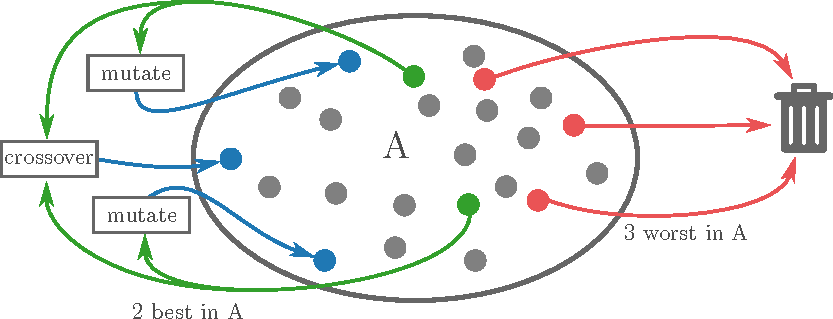
\includegraphics{fig/scenario_a}}
            \caption{Setup 1}
        \end{subfigure} & 
        \begin{subfigure}[t]{\linewidth}
            \resizebox{\textwidth}{!}{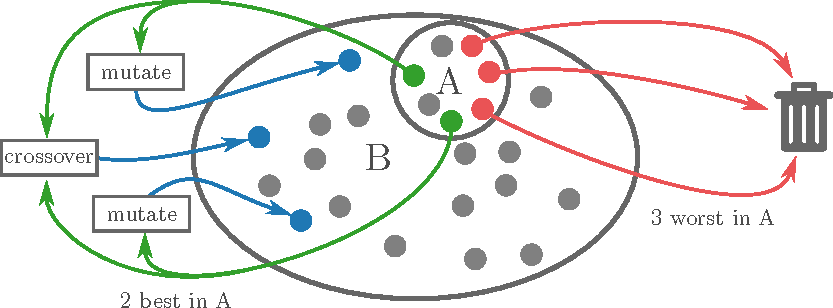
\includegraphics{fig/scenario_b}} 
            \caption{Setup 2}
        \end{subfigure} \\
        \begin{subfigure}[t]{\linewidth}
            \resizebox{\textwidth}{!}{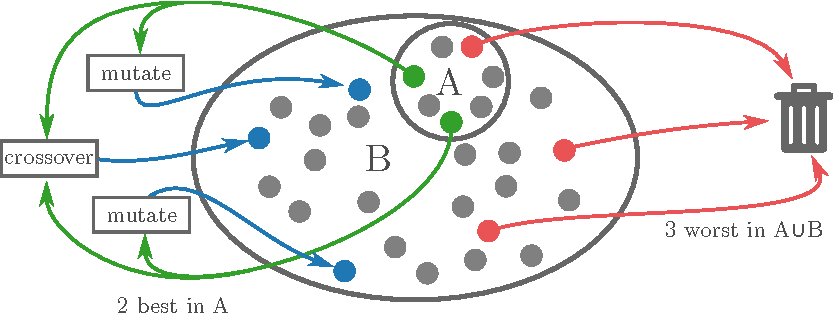
\includegraphics{fig/scenario_c}}
            \caption{Setup 3 (used for main experimental results)}
        \end{subfigure} &
        \begin{subfigure}[t]{\linewidth}
            \resizebox{\textwidth}{!}{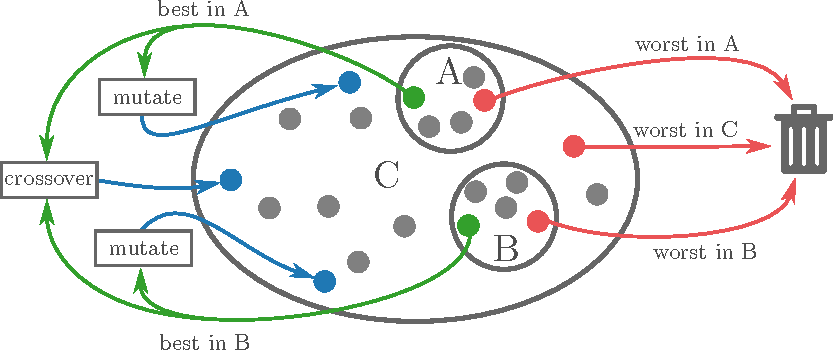
\includegraphics{fig/scenario_d}}
            \caption{Setup 4}
        \end{subfigure}
    \end{tabular}
    \caption{Various genetic algorithm setups compatible with ZCP-based NAS. Identifying favorable algorithmic design choices allows for fair comparison of ZCPs.}
    \label{fig_genetic_setups}
\end{figure}

When designing the genetic search of a zero-cost method, there are many options available. Most prior methods \citep{peng2024swap,lin2021zen,li2023zico} have opted for some form of tournament selection. However, the exact impact of algorithmic design choices within the frame of tournament selection has not been extensively studied.

In this section, we evaluate the performance of state-of-the-art ZCPs under various genetic setups inspired by common design choices encountered in the literature. We identify 4 different scenarii to evaluate which components of the tournament selection framework are integral to a ZCP method's performance. Graphic representations of each setup are also depicted in Fig.~\ref{fig_genetic_setups}:
\begin{itemize}
\item Setup 1: no tournament selection. At each evolutionary step, the 2 best architectures in the whole population go on to mutation and crossover while the 3 worst architectures are discarded. Even before running any experiments, the lack of stochasticity of this scenario is questionable and could lead to early collapse in local minima.
\item Setup 2: full tournament selection. At each evolutionary step, tournament selection is conducted on a subset of the population. The 2 best architectures in the subset go on to mutation and crossover while the 3 worst architectures in the subset are discarded.
\item Setup 3: partial tournament selection. At each evolutionary step, tournament selection is conducted on a subset of the population. Compared to setup 2, the worst 3 architectures across the whole population are discarded, increasing the likelihood of low quality candidates being removed from the genetic pool in early stages. This is the genetic setup used throughout our main experiments.
\item Setup 4: partial multi-tournament selection. At each evolutionary step, tournament selection is conducted separately on 2 subsets of the population. Winners of both subsets undergo mutation and crossover with each other. Discarded architectures are selected from both tournaments and the remainder of the population.
\end{itemize}

\begin{table}[h]
\centering
\caption{Maximum accuracy in the population after ZCP evolution in NB201/ImageNet under various genetic setups.}
\begin{adjustbox}{width=0.7\linewidth}
\begin{tabular}{m{2cm} | m{2.1cm} | m{2.1cm} | m{2.1cm} | m{2.1cm}}
    & Setup 1 & Setup 2 & Setup 3 & Setup 4\\
    \hline

    \texttt{synflow} & 44.94 $\pm$ 0.13 & 45.26 $\pm$ 0.05 & \textbf{46.63 $\pm$ 0.59} & 46.41 $\pm$ 0.69\\

    \texttt{swap} & 44.94 $\pm$ 0.13 & 45.26 $\pm$ 0.05 & 46.14 $\pm$ 0.46 & \textbf{46.24 $\pm$ 0.47}\\

    \texttt{meco} & 44.94 $\pm$ 0.13 & 45.26 $\pm$ 0.05 & 45.20 $\pm$ 1.45 & \textbf{45.97 $\pm$ 0.35}\\

\end{tabular}
\end{adjustbox}
\label{table_abla_genetic_max}
\end{table}

\begin{table}[h]
\centering
\caption{Average accuracy in the population after ZCP evolution in NB201/ImageNet under various genetic setups.}
\begin{adjustbox}{width=0.7\linewidth}
\begin{tabular}{m{2cm} | m{2.1cm} | m{2.1cm} | m{2.1cm} | m{2.1cm}}
    & Setup 1 & Setup 2 & Setup 3 & Setup 4\\
    \hline

    \texttt{synflow} & 41.03 $\pm$ 0.34 & 39.74 $\pm$ 0.92 & \textbf{41.54 $\pm$ 1.42} & 39.70 $\pm$ 1.71\\

    \texttt{swap} & 41.03 $\pm$ 0.34 & 39.74 $\pm$ 0.92 & 42.31 $\pm$ 0.73 & \textbf{43.09 $\pm$ 0.17}\\

    \texttt{meco} & 41.03 $\pm$ 0.34 & 39.74 $\pm$ 0.92 & \textbf{42.48 $\pm$ 0.81} & 39.83 $\pm$ 1.44\\

\end{tabular}
\end{adjustbox}
\label{table_abla_genetic_avg}
\end{table}

We conduct evolution for 50 evolutionary steps on the NB201/ImageNet task over 3 seeds with the \texttt{synflow}, \texttt{swap} and \texttt{meco} metrics as fitness scores and report the results for maximum and average accuracy of the population in Tables~\ref{table_abla_genetic_max} and~\ref{table_abla_genetic_avg}. We observe that setups 1 and 2 produce worse results than setups 3 and 4 overall. More worryingly the evolutions collapse to the exact same populations for a given seed no matter the ZCP, indicating that the design of the genetic algorithm fully overwrites the additional information provided by the metric and leads to a local minimum, thereby creating a performance ceiling. This highlights the importance of proper genetic algorithm design as seemingly small changes (e.g where discarded architectures are selected) can be the difference maker between effective evolution and non-stochastic collapse. Furthermore, setup 4 does not meaningfully improve performance compared to setup 3 based on $1\sigma$ rules, therefore we use setup C in our experiments as it is the least complex of the two.

\section{Conclusion}
\label{conclusion}

In this work, we introduce ParaDis, a framework to associate zero-cost proxies (ZCPs) with space-agnostic parameter-based constraints. We show that our approach brings several benefits for training-free neural architecture search. Through a novel perspective on benchmarking, we identify the inability of ZCPs to correlate with the ranking of the best architectures in the space as the top rank gap and show that ParaDis improves this ongoing issue of the literature by enabling all proxies to reach suitable regions of the space. Concurrently, we show that ParaDis enables the construction of a fully data- and space- agnostic pipeline which can compete with other state-of-the-art methods on the DARTS search space. Owing to its orthogonality with ZCP design and lack of assumptions on the search space, ParaDis is a robust and versatile framework for zero-shot NAS.

%%%
%%%\subsubsection*{Acknowledgments}
%%%Use unnumbered third level headings for the acknowledgments. All
%%%acknowledgments, including those to funding agencies, go at the end of the paper.
%%%Only add this information once your submission is accepted and deanonymized.
%%%

\newpage

\bibliography{bibliography}
\bibliographystyle{tmlr}

\newpage

\appendix

\section{Full ParaDis algorithm}
\label{apx_algorithm}

\begin{algorithm}[ht]
\caption{\underline{\textbf{Para}}meter \underline{\textbf{Dis}}tribution Shift NAS (\textbf{ParaDis})}
\label{alg_paradis}
\begin{algorithmic}[1]
\Require: population size $P$, sample size $p < P/2$, number of generations $N$, evolution steps per generation $S$, zero-cost metric $\mathcal{M}$, temperature schedule $[\tau_0, \tau_1, \dots, \tau_N]$
\State $population \gets \emptyset$
\While {$population.size < P$}
\State Randomly sample $arch$ from the space
\State $arch.zcp\_score \gets \mathcal{M}(arch)$
\State $arch.params \gets CountParams(arch)$
\State Add $arch$ to $population$
\EndWhile
\State $\mu$, $\sigma \gets Mean(population.params), STD(population.params)$
\For {$arch$ in $population$}
\State $arch.paradis\_score \gets \Phi(arch.params, \mu, \sigma, \tau_0)$ \ref{method}
\EndFor
\For {$n=1,2,\dots,N$}
\State $\tau \gets \tau_n$
\For {$s=1,2,\dots S$}
\State Discard 3 worst $archs$ from $population$ by $paradis\_score$
\State $candidates_A \gets p$ random $archs$ of $population$
\State $candidates_B \gets$ all remaining $archs$ in $population$
\State Create children by mutation from best $archs$ in $candidates_A$ and $candidates_B$ by $zcp\_score$
\State Create child by crossover between best $archs$ in $candidates_A$ and $candidates_B$ by $zcp\_score$
\State Compute $zcp\_score$ and $params$ for new children
\State Add children to $population$
\EndFor
\State $\mu$, $\sigma \gets Mean(population.params), STD(population.params)$
\For {$arch$ in $population$}
\State $arch.paradis\_score \gets \Phi(arch.params, \mu, \sigma, \tau)$ \ref{method}
\EndFor
\EndFor
\end{algorithmic}
\end{algorithm}

\section{Additional ablations}

In the following sections, we extensively study the impact of the various hyperparameters on the outcome of our method. Where applicable, we conduct ablation studies using the \texttt{synflow} metric on the NB201 ImageNet16-120 task. Note that the set of hyperparameters obtained for \texttt{synflow} is not necessarily optimal for all other ZCPs. Therefore, we assume fairness in benchmarking ZCPs with the same evolutionary budget.

\subsubsection{Temperature schedule}

\begin{figure}[h]
\centering
\begin{adjustbox}{width=.8\linewidth}
    \begin{subfigure}[t]{.4\textwidth}
        \resizebox{\textwidth}{!}{%% Creator: Matplotlib, PGF backend
%%
%% To include the figure in your LaTeX document, write
%%   \input{<filename>.pgf}
%%
%% Make sure the required packages are loaded in your preamble
%%   \usepackage{pgf}
%%
%% Also ensure that all the required font packages are loaded; for instance,
%% the lmodern package is sometimes necessary when using math font.
%%   \usepackage{lmodern}
%%
%% Figures using additional raster images can only be included by \input if
%% they are in the same directory as the main LaTeX file. For loading figures
%% from other directories you can use the `import` package
%%   \usepackage{import}
%%
%% and then include the figures with
%%   \import{<path to file>}{<filename>.pgf}
%%
%% Matplotlib used the following preamble
%%   
%%   \usepackage{fontspec}
%%   \setmainfont{DejaVuSerif.ttf}[Path=\detokenize{/home/t19lyman/.local/lib/python3.10/site-packages/matplotlib/mpl-data/fonts/ttf/}]
%%   \setsansfont{DejaVuSans.ttf}[Path=\detokenize{/home/t19lyman/.local/lib/python3.10/site-packages/matplotlib/mpl-data/fonts/ttf/}]
%%   \setmonofont{DejaVuSansMono.ttf}[Path=\detokenize{/home/t19lyman/.local/lib/python3.10/site-packages/matplotlib/mpl-data/fonts/ttf/}]
%%   \makeatletter\@ifpackageloaded{underscore}{}{\usepackage[strings]{underscore}}\makeatother
%%
\begingroup%
\makeatletter%
\begin{pgfpicture}%
\pgfpathrectangle{\pgfpointorigin}{\pgfqpoint{6.400000in}{4.800000in}}%
\pgfusepath{use as bounding box, clip}%
\begin{pgfscope}%
\pgfsetbuttcap%
\pgfsetmiterjoin%
\definecolor{currentfill}{rgb}{1.000000,1.000000,1.000000}%
\pgfsetfillcolor{currentfill}%
\pgfsetlinewidth{0.000000pt}%
\definecolor{currentstroke}{rgb}{1.000000,1.000000,1.000000}%
\pgfsetstrokecolor{currentstroke}%
\pgfsetdash{}{0pt}%
\pgfpathmoveto{\pgfqpoint{0.000000in}{0.000000in}}%
\pgfpathlineto{\pgfqpoint{6.400000in}{0.000000in}}%
\pgfpathlineto{\pgfqpoint{6.400000in}{4.800000in}}%
\pgfpathlineto{\pgfqpoint{0.000000in}{4.800000in}}%
\pgfpathlineto{\pgfqpoint{0.000000in}{0.000000in}}%
\pgfpathclose%
\pgfusepath{fill}%
\end{pgfscope}%
\begin{pgfscope}%
\pgfsetbuttcap%
\pgfsetmiterjoin%
\definecolor{currentfill}{rgb}{1.000000,1.000000,1.000000}%
\pgfsetfillcolor{currentfill}%
\pgfsetlinewidth{0.000000pt}%
\definecolor{currentstroke}{rgb}{0.000000,0.000000,0.000000}%
\pgfsetstrokecolor{currentstroke}%
\pgfsetstrokeopacity{0.000000}%
\pgfsetdash{}{0pt}%
\pgfpathmoveto{\pgfqpoint{0.800000in}{0.528000in}}%
\pgfpathlineto{\pgfqpoint{4.768000in}{0.528000in}}%
\pgfpathlineto{\pgfqpoint{4.768000in}{4.224000in}}%
\pgfpathlineto{\pgfqpoint{0.800000in}{4.224000in}}%
\pgfpathlineto{\pgfqpoint{0.800000in}{0.528000in}}%
\pgfpathclose%
\pgfusepath{fill}%
\end{pgfscope}%
\begin{pgfscope}%
\pgfpathrectangle{\pgfqpoint{0.800000in}{0.528000in}}{\pgfqpoint{3.968000in}{3.696000in}}%
\pgfusepath{clip}%
\pgfsetbuttcap%
\pgfsetroundjoin%
\definecolor{currentfill}{rgb}{0.203881,0.096087,0.238609}%
\pgfsetfillcolor{currentfill}%
\pgfsetlinewidth{0.000000pt}%
\definecolor{currentstroke}{rgb}{1.000000,1.000000,1.000000}%
\pgfsetstrokecolor{currentstroke}%
\pgfsetdash{}{0pt}%
\pgfpathmoveto{\pgfqpoint{0.800000in}{4.224000in}}%
\pgfpathlineto{\pgfqpoint{1.792000in}{4.224000in}}%
\pgfpathlineto{\pgfqpoint{1.792000in}{3.300000in}}%
\pgfpathlineto{\pgfqpoint{0.800000in}{3.300000in}}%
\pgfpathlineto{\pgfqpoint{0.800000in}{4.224000in}}%
\pgfusepath{fill}%
\end{pgfscope}%
\begin{pgfscope}%
\pgfpathrectangle{\pgfqpoint{0.800000in}{0.528000in}}{\pgfqpoint{3.968000in}{3.696000in}}%
\pgfusepath{clip}%
\pgfsetbuttcap%
\pgfsetroundjoin%
\definecolor{currentfill}{rgb}{0.477697,0.120699,0.349023}%
\pgfsetfillcolor{currentfill}%
\pgfsetlinewidth{0.000000pt}%
\definecolor{currentstroke}{rgb}{1.000000,1.000000,1.000000}%
\pgfsetstrokecolor{currentstroke}%
\pgfsetdash{}{0pt}%
\pgfpathmoveto{\pgfqpoint{1.792000in}{4.224000in}}%
\pgfpathlineto{\pgfqpoint{2.784000in}{4.224000in}}%
\pgfpathlineto{\pgfqpoint{2.784000in}{3.300000in}}%
\pgfpathlineto{\pgfqpoint{1.792000in}{3.300000in}}%
\pgfpathlineto{\pgfqpoint{1.792000in}{4.224000in}}%
\pgfusepath{fill}%
\end{pgfscope}%
\begin{pgfscope}%
\pgfpathrectangle{\pgfqpoint{0.800000in}{0.528000in}}{\pgfqpoint{3.968000in}{3.696000in}}%
\pgfusepath{clip}%
\pgfsetbuttcap%
\pgfsetroundjoin%
\definecolor{currentfill}{rgb}{0.957848,0.512613,0.357119}%
\pgfsetfillcolor{currentfill}%
\pgfsetlinewidth{0.000000pt}%
\definecolor{currentstroke}{rgb}{1.000000,1.000000,1.000000}%
\pgfsetstrokecolor{currentstroke}%
\pgfsetdash{}{0pt}%
\pgfpathmoveto{\pgfqpoint{2.784000in}{4.224000in}}%
\pgfpathlineto{\pgfqpoint{3.776000in}{4.224000in}}%
\pgfpathlineto{\pgfqpoint{3.776000in}{3.300000in}}%
\pgfpathlineto{\pgfqpoint{2.784000in}{3.300000in}}%
\pgfpathlineto{\pgfqpoint{2.784000in}{4.224000in}}%
\pgfusepath{fill}%
\end{pgfscope}%
\begin{pgfscope}%
\pgfpathrectangle{\pgfqpoint{0.800000in}{0.528000in}}{\pgfqpoint{3.968000in}{3.696000in}}%
\pgfusepath{clip}%
\pgfsetbuttcap%
\pgfsetroundjoin%
\definecolor{currentfill}{rgb}{0.962018,0.586477,0.424918}%
\pgfsetfillcolor{currentfill}%
\pgfsetlinewidth{0.000000pt}%
\definecolor{currentstroke}{rgb}{1.000000,1.000000,1.000000}%
\pgfsetstrokecolor{currentstroke}%
\pgfsetdash{}{0pt}%
\pgfpathmoveto{\pgfqpoint{3.776000in}{4.224000in}}%
\pgfpathlineto{\pgfqpoint{4.768000in}{4.224000in}}%
\pgfpathlineto{\pgfqpoint{4.768000in}{3.300000in}}%
\pgfpathlineto{\pgfqpoint{3.776000in}{3.300000in}}%
\pgfpathlineto{\pgfqpoint{3.776000in}{4.224000in}}%
\pgfusepath{fill}%
\end{pgfscope}%
\begin{pgfscope}%
\pgfpathrectangle{\pgfqpoint{0.800000in}{0.528000in}}{\pgfqpoint{3.968000in}{3.696000in}}%
\pgfusepath{clip}%
\pgfsetbuttcap%
\pgfsetroundjoin%
\definecolor{currentfill}{rgb}{0.239289,0.103826,0.260494}%
\pgfsetfillcolor{currentfill}%
\pgfsetlinewidth{0.000000pt}%
\definecolor{currentstroke}{rgb}{1.000000,1.000000,1.000000}%
\pgfsetstrokecolor{currentstroke}%
\pgfsetdash{}{0pt}%
\pgfpathmoveto{\pgfqpoint{0.800000in}{3.300000in}}%
\pgfpathlineto{\pgfqpoint{1.792000in}{3.300000in}}%
\pgfpathlineto{\pgfqpoint{1.792000in}{2.376000in}}%
\pgfpathlineto{\pgfqpoint{0.800000in}{2.376000in}}%
\pgfpathlineto{\pgfqpoint{0.800000in}{3.300000in}}%
\pgfusepath{fill}%
\end{pgfscope}%
\begin{pgfscope}%
\pgfpathrectangle{\pgfqpoint{0.800000in}{0.528000in}}{\pgfqpoint{3.968000in}{3.696000in}}%
\pgfusepath{clip}%
\pgfsetbuttcap%
\pgfsetroundjoin%
\definecolor{currentfill}{rgb}{0.393645,0.121143,0.329105}%
\pgfsetfillcolor{currentfill}%
\pgfsetlinewidth{0.000000pt}%
\definecolor{currentstroke}{rgb}{1.000000,1.000000,1.000000}%
\pgfsetstrokecolor{currentstroke}%
\pgfsetdash{}{0pt}%
\pgfpathmoveto{\pgfqpoint{1.792000in}{3.300000in}}%
\pgfpathlineto{\pgfqpoint{2.784000in}{3.300000in}}%
\pgfpathlineto{\pgfqpoint{2.784000in}{2.376000in}}%
\pgfpathlineto{\pgfqpoint{1.792000in}{2.376000in}}%
\pgfpathlineto{\pgfqpoint{1.792000in}{3.300000in}}%
\pgfusepath{fill}%
\end{pgfscope}%
\begin{pgfscope}%
\pgfpathrectangle{\pgfqpoint{0.800000in}{0.528000in}}{\pgfqpoint{3.968000in}{3.696000in}}%
\pgfusepath{clip}%
\pgfsetbuttcap%
\pgfsetroundjoin%
\definecolor{currentfill}{rgb}{0.963190,0.619109,0.458249}%
\pgfsetfillcolor{currentfill}%
\pgfsetlinewidth{0.000000pt}%
\definecolor{currentstroke}{rgb}{1.000000,1.000000,1.000000}%
\pgfsetstrokecolor{currentstroke}%
\pgfsetdash{}{0pt}%
\pgfpathmoveto{\pgfqpoint{2.784000in}{3.300000in}}%
\pgfpathlineto{\pgfqpoint{3.776000in}{3.300000in}}%
\pgfpathlineto{\pgfqpoint{3.776000in}{2.376000in}}%
\pgfpathlineto{\pgfqpoint{2.784000in}{2.376000in}}%
\pgfpathlineto{\pgfqpoint{2.784000in}{3.300000in}}%
\pgfusepath{fill}%
\end{pgfscope}%
\begin{pgfscope}%
\pgfpathrectangle{\pgfqpoint{0.800000in}{0.528000in}}{\pgfqpoint{3.968000in}{3.696000in}}%
\pgfusepath{clip}%
\pgfsetbuttcap%
\pgfsetroundjoin%
\definecolor{currentfill}{rgb}{0.953816,0.463738,0.317699}%
\pgfsetfillcolor{currentfill}%
\pgfsetlinewidth{0.000000pt}%
\definecolor{currentstroke}{rgb}{1.000000,1.000000,1.000000}%
\pgfsetstrokecolor{currentstroke}%
\pgfsetdash{}{0pt}%
\pgfpathmoveto{\pgfqpoint{3.776000in}{3.300000in}}%
\pgfpathlineto{\pgfqpoint{4.768000in}{3.300000in}}%
\pgfpathlineto{\pgfqpoint{4.768000in}{2.376000in}}%
\pgfpathlineto{\pgfqpoint{3.776000in}{2.376000in}}%
\pgfpathlineto{\pgfqpoint{3.776000in}{3.300000in}}%
\pgfusepath{fill}%
\end{pgfscope}%
\begin{pgfscope}%
\pgfpathrectangle{\pgfqpoint{0.800000in}{0.528000in}}{\pgfqpoint{3.968000in}{3.696000in}}%
\pgfusepath{clip}%
\pgfsetbuttcap%
\pgfsetroundjoin%
\definecolor{currentfill}{rgb}{0.010608,0.018082,0.100187}%
\pgfsetfillcolor{currentfill}%
\pgfsetlinewidth{0.000000pt}%
\definecolor{currentstroke}{rgb}{1.000000,1.000000,1.000000}%
\pgfsetstrokecolor{currentstroke}%
\pgfsetdash{}{0pt}%
\pgfpathmoveto{\pgfqpoint{0.800000in}{2.376000in}}%
\pgfpathlineto{\pgfqpoint{1.792000in}{2.376000in}}%
\pgfpathlineto{\pgfqpoint{1.792000in}{1.452000in}}%
\pgfpathlineto{\pgfqpoint{0.800000in}{1.452000in}}%
\pgfpathlineto{\pgfqpoint{0.800000in}{2.376000in}}%
\pgfusepath{fill}%
\end{pgfscope}%
\begin{pgfscope}%
\pgfpathrectangle{\pgfqpoint{0.800000in}{0.528000in}}{\pgfqpoint{3.968000in}{3.696000in}}%
\pgfusepath{clip}%
\pgfsetbuttcap%
\pgfsetroundjoin%
\definecolor{currentfill}{rgb}{0.870791,0.179821,0.267974}%
\pgfsetfillcolor{currentfill}%
\pgfsetlinewidth{0.000000pt}%
\definecolor{currentstroke}{rgb}{1.000000,1.000000,1.000000}%
\pgfsetstrokecolor{currentstroke}%
\pgfsetdash{}{0pt}%
\pgfpathmoveto{\pgfqpoint{1.792000in}{2.376000in}}%
\pgfpathlineto{\pgfqpoint{2.784000in}{2.376000in}}%
\pgfpathlineto{\pgfqpoint{2.784000in}{1.452000in}}%
\pgfpathlineto{\pgfqpoint{1.792000in}{1.452000in}}%
\pgfpathlineto{\pgfqpoint{1.792000in}{2.376000in}}%
\pgfusepath{fill}%
\end{pgfscope}%
\begin{pgfscope}%
\pgfpathrectangle{\pgfqpoint{0.800000in}{0.528000in}}{\pgfqpoint{3.968000in}{3.696000in}}%
\pgfusepath{clip}%
\pgfsetbuttcap%
\pgfsetroundjoin%
\definecolor{currentfill}{rgb}{0.967092,0.768560,0.642079}%
\pgfsetfillcolor{currentfill}%
\pgfsetlinewidth{0.000000pt}%
\definecolor{currentstroke}{rgb}{1.000000,1.000000,1.000000}%
\pgfsetstrokecolor{currentstroke}%
\pgfsetdash{}{0pt}%
\pgfpathmoveto{\pgfqpoint{2.784000in}{2.376000in}}%
\pgfpathlineto{\pgfqpoint{3.776000in}{2.376000in}}%
\pgfpathlineto{\pgfqpoint{3.776000in}{1.452000in}}%
\pgfpathlineto{\pgfqpoint{2.784000in}{1.452000in}}%
\pgfpathlineto{\pgfqpoint{2.784000in}{2.376000in}}%
\pgfusepath{fill}%
\end{pgfscope}%
\begin{pgfscope}%
\pgfpathrectangle{\pgfqpoint{0.800000in}{0.528000in}}{\pgfqpoint{3.968000in}{3.696000in}}%
\pgfusepath{clip}%
\pgfsetbuttcap%
\pgfsetroundjoin%
\definecolor{currentfill}{rgb}{0.971694,0.833208,0.737161}%
\pgfsetfillcolor{currentfill}%
\pgfsetlinewidth{0.000000pt}%
\definecolor{currentstroke}{rgb}{1.000000,1.000000,1.000000}%
\pgfsetstrokecolor{currentstroke}%
\pgfsetdash{}{0pt}%
\pgfpathmoveto{\pgfqpoint{3.776000in}{2.376000in}}%
\pgfpathlineto{\pgfqpoint{4.768000in}{2.376000in}}%
\pgfpathlineto{\pgfqpoint{4.768000in}{1.452000in}}%
\pgfpathlineto{\pgfqpoint{3.776000in}{1.452000in}}%
\pgfpathlineto{\pgfqpoint{3.776000in}{2.376000in}}%
\pgfusepath{fill}%
\end{pgfscope}%
\begin{pgfscope}%
\pgfpathrectangle{\pgfqpoint{0.800000in}{0.528000in}}{\pgfqpoint{3.968000in}{3.696000in}}%
\pgfusepath{clip}%
\pgfsetbuttcap%
\pgfsetroundjoin%
\definecolor{currentfill}{rgb}{0.717551,0.087162,0.341300}%
\pgfsetfillcolor{currentfill}%
\pgfsetlinewidth{0.000000pt}%
\definecolor{currentstroke}{rgb}{1.000000,1.000000,1.000000}%
\pgfsetstrokecolor{currentstroke}%
\pgfsetdash{}{0pt}%
\pgfpathmoveto{\pgfqpoint{0.800000in}{1.452000in}}%
\pgfpathlineto{\pgfqpoint{1.792000in}{1.452000in}}%
\pgfpathlineto{\pgfqpoint{1.792000in}{0.528000in}}%
\pgfpathlineto{\pgfqpoint{0.800000in}{0.528000in}}%
\pgfpathlineto{\pgfqpoint{0.800000in}{1.452000in}}%
\pgfusepath{fill}%
\end{pgfscope}%
\begin{pgfscope}%
\pgfpathrectangle{\pgfqpoint{0.800000in}{0.528000in}}{\pgfqpoint{3.968000in}{3.696000in}}%
\pgfusepath{clip}%
\pgfsetbuttcap%
\pgfsetroundjoin%
\definecolor{currentfill}{rgb}{0.911533,0.252926,0.244703}%
\pgfsetfillcolor{currentfill}%
\pgfsetlinewidth{0.000000pt}%
\definecolor{currentstroke}{rgb}{1.000000,1.000000,1.000000}%
\pgfsetstrokecolor{currentstroke}%
\pgfsetdash{}{0pt}%
\pgfpathmoveto{\pgfqpoint{1.792000in}{1.452000in}}%
\pgfpathlineto{\pgfqpoint{2.784000in}{1.452000in}}%
\pgfpathlineto{\pgfqpoint{2.784000in}{0.528000in}}%
\pgfpathlineto{\pgfqpoint{1.792000in}{0.528000in}}%
\pgfpathlineto{\pgfqpoint{1.792000in}{1.452000in}}%
\pgfusepath{fill}%
\end{pgfscope}%
\begin{pgfscope}%
\pgfpathrectangle{\pgfqpoint{0.800000in}{0.528000in}}{\pgfqpoint{3.968000in}{3.696000in}}%
\pgfusepath{clip}%
\pgfsetbuttcap%
\pgfsetroundjoin%
\definecolor{currentfill}{rgb}{0.970718,0.821518,0.719872}%
\pgfsetfillcolor{currentfill}%
\pgfsetlinewidth{0.000000pt}%
\definecolor{currentstroke}{rgb}{1.000000,1.000000,1.000000}%
\pgfsetstrokecolor{currentstroke}%
\pgfsetdash{}{0pt}%
\pgfpathmoveto{\pgfqpoint{2.784000in}{1.452000in}}%
\pgfpathlineto{\pgfqpoint{3.776000in}{1.452000in}}%
\pgfpathlineto{\pgfqpoint{3.776000in}{0.528000in}}%
\pgfpathlineto{\pgfqpoint{2.784000in}{0.528000in}}%
\pgfpathlineto{\pgfqpoint{2.784000in}{1.452000in}}%
\pgfusepath{fill}%
\end{pgfscope}%
\begin{pgfscope}%
\pgfpathrectangle{\pgfqpoint{0.800000in}{0.528000in}}{\pgfqpoint{3.968000in}{3.696000in}}%
\pgfusepath{clip}%
\pgfsetbuttcap%
\pgfsetroundjoin%
\definecolor{currentfill}{rgb}{0.981377,0.920617,0.865369}%
\pgfsetfillcolor{currentfill}%
\pgfsetlinewidth{0.000000pt}%
\definecolor{currentstroke}{rgb}{1.000000,1.000000,1.000000}%
\pgfsetstrokecolor{currentstroke}%
\pgfsetdash{}{0pt}%
\pgfpathmoveto{\pgfqpoint{3.776000in}{1.452000in}}%
\pgfpathlineto{\pgfqpoint{4.768000in}{1.452000in}}%
\pgfpathlineto{\pgfqpoint{4.768000in}{0.528000in}}%
\pgfpathlineto{\pgfqpoint{3.776000in}{0.528000in}}%
\pgfpathlineto{\pgfqpoint{3.776000in}{1.452000in}}%
\pgfusepath{fill}%
\end{pgfscope}%
\begin{pgfscope}%
\pgfsetbuttcap%
\pgfsetroundjoin%
\definecolor{currentfill}{rgb}{0.000000,0.000000,0.000000}%
\pgfsetfillcolor{currentfill}%
\pgfsetlinewidth{0.803000pt}%
\definecolor{currentstroke}{rgb}{0.000000,0.000000,0.000000}%
\pgfsetstrokecolor{currentstroke}%
\pgfsetdash{}{0pt}%
\pgfsys@defobject{currentmarker}{\pgfqpoint{0.000000in}{-0.048611in}}{\pgfqpoint{0.000000in}{0.000000in}}{%
\pgfpathmoveto{\pgfqpoint{0.000000in}{0.000000in}}%
\pgfpathlineto{\pgfqpoint{0.000000in}{-0.048611in}}%
\pgfusepath{stroke,fill}%
}%
\begin{pgfscope}%
\pgfsys@transformshift{1.296000in}{0.528000in}%
\pgfsys@useobject{currentmarker}{}%
\end{pgfscope}%
\end{pgfscope}%
\begin{pgfscope}%
\definecolor{textcolor}{rgb}{0.000000,0.000000,0.000000}%
\pgfsetstrokecolor{textcolor}%
\pgfsetfillcolor{textcolor}%
\pgftext[x=1.296000in,y=0.430778in,,top]{\color{textcolor}\sffamily\fontsize{10.000000}{12.000000}\selectfont 0.5}%
\end{pgfscope}%
\begin{pgfscope}%
\pgfsetbuttcap%
\pgfsetroundjoin%
\definecolor{currentfill}{rgb}{0.000000,0.000000,0.000000}%
\pgfsetfillcolor{currentfill}%
\pgfsetlinewidth{0.803000pt}%
\definecolor{currentstroke}{rgb}{0.000000,0.000000,0.000000}%
\pgfsetstrokecolor{currentstroke}%
\pgfsetdash{}{0pt}%
\pgfsys@defobject{currentmarker}{\pgfqpoint{0.000000in}{-0.048611in}}{\pgfqpoint{0.000000in}{0.000000in}}{%
\pgfpathmoveto{\pgfqpoint{0.000000in}{0.000000in}}%
\pgfpathlineto{\pgfqpoint{0.000000in}{-0.048611in}}%
\pgfusepath{stroke,fill}%
}%
\begin{pgfscope}%
\pgfsys@transformshift{2.288000in}{0.528000in}%
\pgfsys@useobject{currentmarker}{}%
\end{pgfscope}%
\end{pgfscope}%
\begin{pgfscope}%
\definecolor{textcolor}{rgb}{0.000000,0.000000,0.000000}%
\pgfsetstrokecolor{textcolor}%
\pgfsetfillcolor{textcolor}%
\pgftext[x=2.288000in,y=0.430778in,,top]{\color{textcolor}\sffamily\fontsize{10.000000}{12.000000}\selectfont 1.0}%
\end{pgfscope}%
\begin{pgfscope}%
\pgfsetbuttcap%
\pgfsetroundjoin%
\definecolor{currentfill}{rgb}{0.000000,0.000000,0.000000}%
\pgfsetfillcolor{currentfill}%
\pgfsetlinewidth{0.803000pt}%
\definecolor{currentstroke}{rgb}{0.000000,0.000000,0.000000}%
\pgfsetstrokecolor{currentstroke}%
\pgfsetdash{}{0pt}%
\pgfsys@defobject{currentmarker}{\pgfqpoint{0.000000in}{-0.048611in}}{\pgfqpoint{0.000000in}{0.000000in}}{%
\pgfpathmoveto{\pgfqpoint{0.000000in}{0.000000in}}%
\pgfpathlineto{\pgfqpoint{0.000000in}{-0.048611in}}%
\pgfusepath{stroke,fill}%
}%
\begin{pgfscope}%
\pgfsys@transformshift{3.280000in}{0.528000in}%
\pgfsys@useobject{currentmarker}{}%
\end{pgfscope}%
\end{pgfscope}%
\begin{pgfscope}%
\definecolor{textcolor}{rgb}{0.000000,0.000000,0.000000}%
\pgfsetstrokecolor{textcolor}%
\pgfsetfillcolor{textcolor}%
\pgftext[x=3.280000in,y=0.430778in,,top]{\color{textcolor}\sffamily\fontsize{10.000000}{12.000000}\selectfont 1.5}%
\end{pgfscope}%
\begin{pgfscope}%
\pgfsetbuttcap%
\pgfsetroundjoin%
\definecolor{currentfill}{rgb}{0.000000,0.000000,0.000000}%
\pgfsetfillcolor{currentfill}%
\pgfsetlinewidth{0.803000pt}%
\definecolor{currentstroke}{rgb}{0.000000,0.000000,0.000000}%
\pgfsetstrokecolor{currentstroke}%
\pgfsetdash{}{0pt}%
\pgfsys@defobject{currentmarker}{\pgfqpoint{0.000000in}{-0.048611in}}{\pgfqpoint{0.000000in}{0.000000in}}{%
\pgfpathmoveto{\pgfqpoint{0.000000in}{0.000000in}}%
\pgfpathlineto{\pgfqpoint{0.000000in}{-0.048611in}}%
\pgfusepath{stroke,fill}%
}%
\begin{pgfscope}%
\pgfsys@transformshift{4.272000in}{0.528000in}%
\pgfsys@useobject{currentmarker}{}%
\end{pgfscope}%
\end{pgfscope}%
\begin{pgfscope}%
\definecolor{textcolor}{rgb}{0.000000,0.000000,0.000000}%
\pgfsetstrokecolor{textcolor}%
\pgfsetfillcolor{textcolor}%
\pgftext[x=4.272000in,y=0.430778in,,top]{\color{textcolor}\sffamily\fontsize{10.000000}{12.000000}\selectfont 2.0}%
\end{pgfscope}%
\begin{pgfscope}%
\definecolor{textcolor}{rgb}{0.000000,0.000000,0.000000}%
\pgfsetstrokecolor{textcolor}%
\pgfsetfillcolor{textcolor}%
\pgftext[x=2.784000in,y=0.240809in,,top]{\color{textcolor}\sffamily\fontsize{10.000000}{12.000000}\selectfont Start $\tau$}%
\end{pgfscope}%
\begin{pgfscope}%
\pgfsetbuttcap%
\pgfsetroundjoin%
\definecolor{currentfill}{rgb}{0.000000,0.000000,0.000000}%
\pgfsetfillcolor{currentfill}%
\pgfsetlinewidth{0.803000pt}%
\definecolor{currentstroke}{rgb}{0.000000,0.000000,0.000000}%
\pgfsetstrokecolor{currentstroke}%
\pgfsetdash{}{0pt}%
\pgfsys@defobject{currentmarker}{\pgfqpoint{-0.048611in}{0.000000in}}{\pgfqpoint{-0.000000in}{0.000000in}}{%
\pgfpathmoveto{\pgfqpoint{-0.000000in}{0.000000in}}%
\pgfpathlineto{\pgfqpoint{-0.048611in}{0.000000in}}%
\pgfusepath{stroke,fill}%
}%
\begin{pgfscope}%
\pgfsys@transformshift{0.800000in}{3.762000in}%
\pgfsys@useobject{currentmarker}{}%
\end{pgfscope}%
\end{pgfscope}%
\begin{pgfscope}%
\definecolor{textcolor}{rgb}{0.000000,0.000000,0.000000}%
\pgfsetstrokecolor{textcolor}%
\pgfsetfillcolor{textcolor}%
\pgftext[x=0.673888in, y=3.626502in, left, base,rotate=90.000000]{\color{textcolor}\sffamily\fontsize{10.000000}{12.000000}\selectfont -2.0}%
\end{pgfscope}%
\begin{pgfscope}%
\pgfsetbuttcap%
\pgfsetroundjoin%
\definecolor{currentfill}{rgb}{0.000000,0.000000,0.000000}%
\pgfsetfillcolor{currentfill}%
\pgfsetlinewidth{0.803000pt}%
\definecolor{currentstroke}{rgb}{0.000000,0.000000,0.000000}%
\pgfsetstrokecolor{currentstroke}%
\pgfsetdash{}{0pt}%
\pgfsys@defobject{currentmarker}{\pgfqpoint{-0.048611in}{0.000000in}}{\pgfqpoint{-0.000000in}{0.000000in}}{%
\pgfpathmoveto{\pgfqpoint{-0.000000in}{0.000000in}}%
\pgfpathlineto{\pgfqpoint{-0.048611in}{0.000000in}}%
\pgfusepath{stroke,fill}%
}%
\begin{pgfscope}%
\pgfsys@transformshift{0.800000in}{2.838000in}%
\pgfsys@useobject{currentmarker}{}%
\end{pgfscope}%
\end{pgfscope}%
\begin{pgfscope}%
\definecolor{textcolor}{rgb}{0.000000,0.000000,0.000000}%
\pgfsetstrokecolor{textcolor}%
\pgfsetfillcolor{textcolor}%
\pgftext[x=0.673888in, y=2.702502in, left, base,rotate=90.000000]{\color{textcolor}\sffamily\fontsize{10.000000}{12.000000}\selectfont -1.5}%
\end{pgfscope}%
\begin{pgfscope}%
\pgfsetbuttcap%
\pgfsetroundjoin%
\definecolor{currentfill}{rgb}{0.000000,0.000000,0.000000}%
\pgfsetfillcolor{currentfill}%
\pgfsetlinewidth{0.803000pt}%
\definecolor{currentstroke}{rgb}{0.000000,0.000000,0.000000}%
\pgfsetstrokecolor{currentstroke}%
\pgfsetdash{}{0pt}%
\pgfsys@defobject{currentmarker}{\pgfqpoint{-0.048611in}{0.000000in}}{\pgfqpoint{-0.000000in}{0.000000in}}{%
\pgfpathmoveto{\pgfqpoint{-0.000000in}{0.000000in}}%
\pgfpathlineto{\pgfqpoint{-0.048611in}{0.000000in}}%
\pgfusepath{stroke,fill}%
}%
\begin{pgfscope}%
\pgfsys@transformshift{0.800000in}{1.914000in}%
\pgfsys@useobject{currentmarker}{}%
\end{pgfscope}%
\end{pgfscope}%
\begin{pgfscope}%
\definecolor{textcolor}{rgb}{0.000000,0.000000,0.000000}%
\pgfsetstrokecolor{textcolor}%
\pgfsetfillcolor{textcolor}%
\pgftext[x=0.673888in, y=1.778502in, left, base,rotate=90.000000]{\color{textcolor}\sffamily\fontsize{10.000000}{12.000000}\selectfont -1.0}%
\end{pgfscope}%
\begin{pgfscope}%
\pgfsetbuttcap%
\pgfsetroundjoin%
\definecolor{currentfill}{rgb}{0.000000,0.000000,0.000000}%
\pgfsetfillcolor{currentfill}%
\pgfsetlinewidth{0.803000pt}%
\definecolor{currentstroke}{rgb}{0.000000,0.000000,0.000000}%
\pgfsetstrokecolor{currentstroke}%
\pgfsetdash{}{0pt}%
\pgfsys@defobject{currentmarker}{\pgfqpoint{-0.048611in}{0.000000in}}{\pgfqpoint{-0.000000in}{0.000000in}}{%
\pgfpathmoveto{\pgfqpoint{-0.000000in}{0.000000in}}%
\pgfpathlineto{\pgfqpoint{-0.048611in}{0.000000in}}%
\pgfusepath{stroke,fill}%
}%
\begin{pgfscope}%
\pgfsys@transformshift{0.800000in}{0.990000in}%
\pgfsys@useobject{currentmarker}{}%
\end{pgfscope}%
\end{pgfscope}%
\begin{pgfscope}%
\definecolor{textcolor}{rgb}{0.000000,0.000000,0.000000}%
\pgfsetstrokecolor{textcolor}%
\pgfsetfillcolor{textcolor}%
\pgftext[x=0.673888in, y=0.854502in, left, base,rotate=90.000000]{\color{textcolor}\sffamily\fontsize{10.000000}{12.000000}\selectfont -0.5}%
\end{pgfscope}%
\begin{pgfscope}%
\definecolor{textcolor}{rgb}{0.000000,0.000000,0.000000}%
\pgfsetstrokecolor{textcolor}%
\pgfsetfillcolor{textcolor}%
\pgftext[x=0.512809in,y=2.376000in,,bottom,rotate=90.000000]{\color{textcolor}\sffamily\fontsize{10.000000}{12.000000}\selectfont End $\tau$}%
\end{pgfscope}%
\begin{pgfscope}%
\pgfsetbuttcap%
\pgfsetmiterjoin%
\definecolor{currentfill}{rgb}{1.000000,1.000000,1.000000}%
\pgfsetfillcolor{currentfill}%
\pgfsetlinewidth{0.000000pt}%
\definecolor{currentstroke}{rgb}{0.000000,0.000000,0.000000}%
\pgfsetstrokecolor{currentstroke}%
\pgfsetstrokeopacity{0.000000}%
\pgfsetdash{}{0pt}%
\pgfpathmoveto{\pgfqpoint{5.016000in}{0.528000in}}%
\pgfpathlineto{\pgfqpoint{5.200800in}{0.528000in}}%
\pgfpathlineto{\pgfqpoint{5.200800in}{4.224000in}}%
\pgfpathlineto{\pgfqpoint{5.016000in}{4.224000in}}%
\pgfpathlineto{\pgfqpoint{5.016000in}{0.528000in}}%
\pgfpathclose%
\pgfusepath{fill}%
\end{pgfscope}%
\begin{pgfscope}%
\pgfsys@transformshift{5.020000in}{0.530000in}%
\pgftext[left,bottom]{
\includegraphics[interpolate=true,width=0.180000in,height=3.690000in]{fig/ablations/heatmap_tau_popmax-img0.png}}%
\end{pgfscope}%
\begin{pgfscope}%
\pgfsetbuttcap%
\pgfsetroundjoin%
\definecolor{currentfill}{rgb}{0.000000,0.000000,0.000000}%
\pgfsetfillcolor{currentfill}%
\pgfsetlinewidth{0.803000pt}%
\definecolor{currentstroke}{rgb}{0.000000,0.000000,0.000000}%
\pgfsetstrokecolor{currentstroke}%
\pgfsetdash{}{0pt}%
\pgfsys@defobject{currentmarker}{\pgfqpoint{0.000000in}{0.000000in}}{\pgfqpoint{0.048611in}{0.000000in}}{%
\pgfpathmoveto{\pgfqpoint{0.000000in}{0.000000in}}%
\pgfpathlineto{\pgfqpoint{0.048611in}{0.000000in}}%
\pgfusepath{stroke,fill}%
}%
\begin{pgfscope}%
\pgfsys@transformshift{5.200800in}{0.657891in}%
\pgfsys@useobject{currentmarker}{}%
\end{pgfscope}%
\end{pgfscope}%
\begin{pgfscope}%
\definecolor{textcolor}{rgb}{0.000000,0.000000,0.000000}%
\pgfsetstrokecolor{textcolor}%
\pgfsetfillcolor{textcolor}%
\pgftext[x=5.298022in, y=0.605130in, left, base]{\color{textcolor}\sffamily\fontsize{10.000000}{12.000000}\selectfont 44.0}%
\end{pgfscope}%
\begin{pgfscope}%
\pgfsetbuttcap%
\pgfsetroundjoin%
\definecolor{currentfill}{rgb}{0.000000,0.000000,0.000000}%
\pgfsetfillcolor{currentfill}%
\pgfsetlinewidth{0.803000pt}%
\definecolor{currentstroke}{rgb}{0.000000,0.000000,0.000000}%
\pgfsetstrokecolor{currentstroke}%
\pgfsetdash{}{0pt}%
\pgfsys@defobject{currentmarker}{\pgfqpoint{0.000000in}{0.000000in}}{\pgfqpoint{0.048611in}{0.000000in}}{%
\pgfpathmoveto{\pgfqpoint{0.000000in}{0.000000in}}%
\pgfpathlineto{\pgfqpoint{0.048611in}{0.000000in}}%
\pgfusepath{stroke,fill}%
}%
\begin{pgfscope}%
\pgfsys@transformshift{5.200800in}{1.248307in}%
\pgfsys@useobject{currentmarker}{}%
\end{pgfscope}%
\end{pgfscope}%
\begin{pgfscope}%
\definecolor{textcolor}{rgb}{0.000000,0.000000,0.000000}%
\pgfsetstrokecolor{textcolor}%
\pgfsetfillcolor{textcolor}%
\pgftext[x=5.298022in, y=1.195545in, left, base]{\color{textcolor}\sffamily\fontsize{10.000000}{12.000000}\selectfont 44.5}%
\end{pgfscope}%
\begin{pgfscope}%
\pgfsetbuttcap%
\pgfsetroundjoin%
\definecolor{currentfill}{rgb}{0.000000,0.000000,0.000000}%
\pgfsetfillcolor{currentfill}%
\pgfsetlinewidth{0.803000pt}%
\definecolor{currentstroke}{rgb}{0.000000,0.000000,0.000000}%
\pgfsetstrokecolor{currentstroke}%
\pgfsetdash{}{0pt}%
\pgfsys@defobject{currentmarker}{\pgfqpoint{0.000000in}{0.000000in}}{\pgfqpoint{0.048611in}{0.000000in}}{%
\pgfpathmoveto{\pgfqpoint{0.000000in}{0.000000in}}%
\pgfpathlineto{\pgfqpoint{0.048611in}{0.000000in}}%
\pgfusepath{stroke,fill}%
}%
\begin{pgfscope}%
\pgfsys@transformshift{5.200800in}{1.838722in}%
\pgfsys@useobject{currentmarker}{}%
\end{pgfscope}%
\end{pgfscope}%
\begin{pgfscope}%
\definecolor{textcolor}{rgb}{0.000000,0.000000,0.000000}%
\pgfsetstrokecolor{textcolor}%
\pgfsetfillcolor{textcolor}%
\pgftext[x=5.298022in, y=1.785961in, left, base]{\color{textcolor}\sffamily\fontsize{10.000000}{12.000000}\selectfont 45.0}%
\end{pgfscope}%
\begin{pgfscope}%
\pgfsetbuttcap%
\pgfsetroundjoin%
\definecolor{currentfill}{rgb}{0.000000,0.000000,0.000000}%
\pgfsetfillcolor{currentfill}%
\pgfsetlinewidth{0.803000pt}%
\definecolor{currentstroke}{rgb}{0.000000,0.000000,0.000000}%
\pgfsetstrokecolor{currentstroke}%
\pgfsetdash{}{0pt}%
\pgfsys@defobject{currentmarker}{\pgfqpoint{0.000000in}{0.000000in}}{\pgfqpoint{0.048611in}{0.000000in}}{%
\pgfpathmoveto{\pgfqpoint{0.000000in}{0.000000in}}%
\pgfpathlineto{\pgfqpoint{0.048611in}{0.000000in}}%
\pgfusepath{stroke,fill}%
}%
\begin{pgfscope}%
\pgfsys@transformshift{5.200800in}{2.429137in}%
\pgfsys@useobject{currentmarker}{}%
\end{pgfscope}%
\end{pgfscope}%
\begin{pgfscope}%
\definecolor{textcolor}{rgb}{0.000000,0.000000,0.000000}%
\pgfsetstrokecolor{textcolor}%
\pgfsetfillcolor{textcolor}%
\pgftext[x=5.298022in, y=2.376376in, left, base]{\color{textcolor}\sffamily\fontsize{10.000000}{12.000000}\selectfont 45.5}%
\end{pgfscope}%
\begin{pgfscope}%
\pgfsetbuttcap%
\pgfsetroundjoin%
\definecolor{currentfill}{rgb}{0.000000,0.000000,0.000000}%
\pgfsetfillcolor{currentfill}%
\pgfsetlinewidth{0.803000pt}%
\definecolor{currentstroke}{rgb}{0.000000,0.000000,0.000000}%
\pgfsetstrokecolor{currentstroke}%
\pgfsetdash{}{0pt}%
\pgfsys@defobject{currentmarker}{\pgfqpoint{0.000000in}{0.000000in}}{\pgfqpoint{0.048611in}{0.000000in}}{%
\pgfpathmoveto{\pgfqpoint{0.000000in}{0.000000in}}%
\pgfpathlineto{\pgfqpoint{0.048611in}{0.000000in}}%
\pgfusepath{stroke,fill}%
}%
\begin{pgfscope}%
\pgfsys@transformshift{5.200800in}{3.019553in}%
\pgfsys@useobject{currentmarker}{}%
\end{pgfscope}%
\end{pgfscope}%
\begin{pgfscope}%
\definecolor{textcolor}{rgb}{0.000000,0.000000,0.000000}%
\pgfsetstrokecolor{textcolor}%
\pgfsetfillcolor{textcolor}%
\pgftext[x=5.298022in, y=2.966791in, left, base]{\color{textcolor}\sffamily\fontsize{10.000000}{12.000000}\selectfont 46.0}%
\end{pgfscope}%
\begin{pgfscope}%
\pgfsetbuttcap%
\pgfsetroundjoin%
\definecolor{currentfill}{rgb}{0.000000,0.000000,0.000000}%
\pgfsetfillcolor{currentfill}%
\pgfsetlinewidth{0.803000pt}%
\definecolor{currentstroke}{rgb}{0.000000,0.000000,0.000000}%
\pgfsetstrokecolor{currentstroke}%
\pgfsetdash{}{0pt}%
\pgfsys@defobject{currentmarker}{\pgfqpoint{0.000000in}{0.000000in}}{\pgfqpoint{0.048611in}{0.000000in}}{%
\pgfpathmoveto{\pgfqpoint{0.000000in}{0.000000in}}%
\pgfpathlineto{\pgfqpoint{0.048611in}{0.000000in}}%
\pgfusepath{stroke,fill}%
}%
\begin{pgfscope}%
\pgfsys@transformshift{5.200800in}{3.609968in}%
\pgfsys@useobject{currentmarker}{}%
\end{pgfscope}%
\end{pgfscope}%
\begin{pgfscope}%
\definecolor{textcolor}{rgb}{0.000000,0.000000,0.000000}%
\pgfsetstrokecolor{textcolor}%
\pgfsetfillcolor{textcolor}%
\pgftext[x=5.298022in, y=3.557207in, left, base]{\color{textcolor}\sffamily\fontsize{10.000000}{12.000000}\selectfont 46.5}%
\end{pgfscope}%
\begin{pgfscope}%
\pgfsetbuttcap%
\pgfsetroundjoin%
\definecolor{currentfill}{rgb}{0.000000,0.000000,0.000000}%
\pgfsetfillcolor{currentfill}%
\pgfsetlinewidth{0.803000pt}%
\definecolor{currentstroke}{rgb}{0.000000,0.000000,0.000000}%
\pgfsetstrokecolor{currentstroke}%
\pgfsetdash{}{0pt}%
\pgfsys@defobject{currentmarker}{\pgfqpoint{0.000000in}{0.000000in}}{\pgfqpoint{0.048611in}{0.000000in}}{%
\pgfpathmoveto{\pgfqpoint{0.000000in}{0.000000in}}%
\pgfpathlineto{\pgfqpoint{0.048611in}{0.000000in}}%
\pgfusepath{stroke,fill}%
}%
\begin{pgfscope}%
\pgfsys@transformshift{5.200800in}{4.200383in}%
\pgfsys@useobject{currentmarker}{}%
\end{pgfscope}%
\end{pgfscope}%
\begin{pgfscope}%
\definecolor{textcolor}{rgb}{0.000000,0.000000,0.000000}%
\pgfsetstrokecolor{textcolor}%
\pgfsetfillcolor{textcolor}%
\pgftext[x=5.298022in, y=4.147622in, left, base]{\color{textcolor}\sffamily\fontsize{10.000000}{12.000000}\selectfont 47.0}%
\end{pgfscope}%
\begin{pgfscope}%
\pgfsetrectcap%
\pgfsetmiterjoin%
\pgfsetlinewidth{0.000000pt}%
\definecolor{currentstroke}{rgb}{0.000000,0.000000,0.000000}%
\pgfsetstrokecolor{currentstroke}%
\pgfsetdash{}{0pt}%
\pgfpathmoveto{\pgfqpoint{5.016000in}{0.528000in}}%
\pgfpathlineto{\pgfqpoint{5.108400in}{0.528000in}}%
\pgfpathlineto{\pgfqpoint{5.200800in}{0.528000in}}%
\pgfpathlineto{\pgfqpoint{5.200800in}{4.224000in}}%
\pgfpathlineto{\pgfqpoint{5.108400in}{4.224000in}}%
\pgfpathlineto{\pgfqpoint{5.016000in}{4.224000in}}%
\pgfpathlineto{\pgfqpoint{5.016000in}{0.528000in}}%
\pgfpathclose%
\pgfusepath{}%
\end{pgfscope}%
\end{pgfpicture}%
\makeatother%
\endgroup%
}
        \caption{\centering Max population accuracy under various start/end $\tau$ pairs.}
        \label{fig_abla_tau_max}
    \end{subfigure}%
    \hfill%
    \begin{subfigure}[t]{.4\textwidth}
        \resizebox{\textwidth}{!}{%% Creator: Matplotlib, PGF backend
%%
%% To include the figure in your LaTeX document, write
%%   \input{<filename>.pgf}
%%
%% Make sure the required packages are loaded in your preamble
%%   \usepackage{pgf}
%%
%% Also ensure that all the required font packages are loaded; for instance,
%% the lmodern package is sometimes necessary when using math font.
%%   \usepackage{lmodern}
%%
%% Figures using additional raster images can only be included by \input if
%% they are in the same directory as the main LaTeX file. For loading figures
%% from other directories you can use the `import` package
%%   \usepackage{import}
%%
%% and then include the figures with
%%   \import{<path to file>}{<filename>.pgf}
%%
%% Matplotlib used the following preamble
%%   
%%   \usepackage{fontspec}
%%   \setmainfont{DejaVuSerif.ttf}[Path=\detokenize{/home/t19lyman/.local/lib/python3.10/site-packages/matplotlib/mpl-data/fonts/ttf/}]
%%   \setsansfont{DejaVuSans.ttf}[Path=\detokenize{/home/t19lyman/.local/lib/python3.10/site-packages/matplotlib/mpl-data/fonts/ttf/}]
%%   \setmonofont{DejaVuSansMono.ttf}[Path=\detokenize{/home/t19lyman/.local/lib/python3.10/site-packages/matplotlib/mpl-data/fonts/ttf/}]
%%   \makeatletter\@ifpackageloaded{underscore}{}{\usepackage[strings]{underscore}}\makeatother
%%
\begingroup%
\makeatletter%
\begin{pgfpicture}%
\pgfpathrectangle{\pgfpointorigin}{\pgfqpoint{6.400000in}{4.800000in}}%
\pgfusepath{use as bounding box, clip}%
\begin{pgfscope}%
\pgfsetbuttcap%
\pgfsetmiterjoin%
\definecolor{currentfill}{rgb}{1.000000,1.000000,1.000000}%
\pgfsetfillcolor{currentfill}%
\pgfsetlinewidth{0.000000pt}%
\definecolor{currentstroke}{rgb}{1.000000,1.000000,1.000000}%
\pgfsetstrokecolor{currentstroke}%
\pgfsetdash{}{0pt}%
\pgfpathmoveto{\pgfqpoint{0.000000in}{0.000000in}}%
\pgfpathlineto{\pgfqpoint{6.400000in}{0.000000in}}%
\pgfpathlineto{\pgfqpoint{6.400000in}{4.800000in}}%
\pgfpathlineto{\pgfqpoint{0.000000in}{4.800000in}}%
\pgfpathlineto{\pgfqpoint{0.000000in}{0.000000in}}%
\pgfpathclose%
\pgfusepath{fill}%
\end{pgfscope}%
\begin{pgfscope}%
\pgfsetbuttcap%
\pgfsetmiterjoin%
\definecolor{currentfill}{rgb}{1.000000,1.000000,1.000000}%
\pgfsetfillcolor{currentfill}%
\pgfsetlinewidth{0.000000pt}%
\definecolor{currentstroke}{rgb}{0.000000,0.000000,0.000000}%
\pgfsetstrokecolor{currentstroke}%
\pgfsetstrokeopacity{0.000000}%
\pgfsetdash{}{0pt}%
\pgfpathmoveto{\pgfqpoint{0.800000in}{0.528000in}}%
\pgfpathlineto{\pgfqpoint{4.768000in}{0.528000in}}%
\pgfpathlineto{\pgfqpoint{4.768000in}{4.224000in}}%
\pgfpathlineto{\pgfqpoint{0.800000in}{4.224000in}}%
\pgfpathlineto{\pgfqpoint{0.800000in}{0.528000in}}%
\pgfpathclose%
\pgfusepath{fill}%
\end{pgfscope}%
\begin{pgfscope}%
\pgfpathrectangle{\pgfqpoint{0.800000in}{0.528000in}}{\pgfqpoint{3.968000in}{3.696000in}}%
\pgfusepath{clip}%
\pgfsetbuttcap%
\pgfsetroundjoin%
\definecolor{currentfill}{rgb}{0.324459,0.116396,0.303694}%
\pgfsetfillcolor{currentfill}%
\pgfsetlinewidth{0.000000pt}%
\definecolor{currentstroke}{rgb}{1.000000,1.000000,1.000000}%
\pgfsetstrokecolor{currentstroke}%
\pgfsetdash{}{0pt}%
\pgfpathmoveto{\pgfqpoint{0.800000in}{4.224000in}}%
\pgfpathlineto{\pgfqpoint{1.792000in}{4.224000in}}%
\pgfpathlineto{\pgfqpoint{1.792000in}{3.300000in}}%
\pgfpathlineto{\pgfqpoint{0.800000in}{3.300000in}}%
\pgfpathlineto{\pgfqpoint{0.800000in}{4.224000in}}%
\pgfusepath{fill}%
\end{pgfscope}%
\begin{pgfscope}%
\pgfpathrectangle{\pgfqpoint{0.800000in}{0.528000in}}{\pgfqpoint{3.968000in}{3.696000in}}%
\pgfusepath{clip}%
\pgfsetbuttcap%
\pgfsetroundjoin%
\definecolor{currentfill}{rgb}{0.245256,0.104974,0.263956}%
\pgfsetfillcolor{currentfill}%
\pgfsetlinewidth{0.000000pt}%
\definecolor{currentstroke}{rgb}{1.000000,1.000000,1.000000}%
\pgfsetstrokecolor{currentstroke}%
\pgfsetdash{}{0pt}%
\pgfpathmoveto{\pgfqpoint{1.792000in}{4.224000in}}%
\pgfpathlineto{\pgfqpoint{2.784000in}{4.224000in}}%
\pgfpathlineto{\pgfqpoint{2.784000in}{3.300000in}}%
\pgfpathlineto{\pgfqpoint{1.792000in}{3.300000in}}%
\pgfpathlineto{\pgfqpoint{1.792000in}{4.224000in}}%
\pgfusepath{fill}%
\end{pgfscope}%
\begin{pgfscope}%
\pgfpathrectangle{\pgfqpoint{0.800000in}{0.528000in}}{\pgfqpoint{3.968000in}{3.696000in}}%
\pgfusepath{clip}%
\pgfsetbuttcap%
\pgfsetroundjoin%
\definecolor{currentfill}{rgb}{0.971694,0.833208,0.737161}%
\pgfsetfillcolor{currentfill}%
\pgfsetlinewidth{0.000000pt}%
\definecolor{currentstroke}{rgb}{1.000000,1.000000,1.000000}%
\pgfsetstrokecolor{currentstroke}%
\pgfsetdash{}{0pt}%
\pgfpathmoveto{\pgfqpoint{2.784000in}{4.224000in}}%
\pgfpathlineto{\pgfqpoint{3.776000in}{4.224000in}}%
\pgfpathlineto{\pgfqpoint{3.776000in}{3.300000in}}%
\pgfpathlineto{\pgfqpoint{2.784000in}{3.300000in}}%
\pgfpathlineto{\pgfqpoint{2.784000in}{4.224000in}}%
\pgfusepath{fill}%
\end{pgfscope}%
\begin{pgfscope}%
\pgfpathrectangle{\pgfqpoint{0.800000in}{0.528000in}}{\pgfqpoint{3.968000in}{3.696000in}}%
\pgfusepath{clip}%
\pgfsetbuttcap%
\pgfsetroundjoin%
\definecolor{currentfill}{rgb}{0.848131,0.150999,0.281943}%
\pgfsetfillcolor{currentfill}%
\pgfsetlinewidth{0.000000pt}%
\definecolor{currentstroke}{rgb}{1.000000,1.000000,1.000000}%
\pgfsetstrokecolor{currentstroke}%
\pgfsetdash{}{0pt}%
\pgfpathmoveto{\pgfqpoint{3.776000in}{4.224000in}}%
\pgfpathlineto{\pgfqpoint{4.768000in}{4.224000in}}%
\pgfpathlineto{\pgfqpoint{4.768000in}{3.300000in}}%
\pgfpathlineto{\pgfqpoint{3.776000in}{3.300000in}}%
\pgfpathlineto{\pgfqpoint{3.776000in}{4.224000in}}%
\pgfusepath{fill}%
\end{pgfscope}%
\begin{pgfscope}%
\pgfpathrectangle{\pgfqpoint{0.800000in}{0.528000in}}{\pgfqpoint{3.968000in}{3.696000in}}%
\pgfusepath{clip}%
\pgfsetbuttcap%
\pgfsetroundjoin%
\definecolor{currentfill}{rgb}{0.419253,0.121738,0.336404}%
\pgfsetfillcolor{currentfill}%
\pgfsetlinewidth{0.000000pt}%
\definecolor{currentstroke}{rgb}{1.000000,1.000000,1.000000}%
\pgfsetstrokecolor{currentstroke}%
\pgfsetdash{}{0pt}%
\pgfpathmoveto{\pgfqpoint{0.800000in}{3.300000in}}%
\pgfpathlineto{\pgfqpoint{1.792000in}{3.300000in}}%
\pgfpathlineto{\pgfqpoint{1.792000in}{2.376000in}}%
\pgfpathlineto{\pgfqpoint{0.800000in}{2.376000in}}%
\pgfpathlineto{\pgfqpoint{0.800000in}{3.300000in}}%
\pgfusepath{fill}%
\end{pgfscope}%
\begin{pgfscope}%
\pgfpathrectangle{\pgfqpoint{0.800000in}{0.528000in}}{\pgfqpoint{3.968000in}{3.696000in}}%
\pgfusepath{clip}%
\pgfsetbuttcap%
\pgfsetroundjoin%
\definecolor{currentfill}{rgb}{0.471148,0.120987,0.347880}%
\pgfsetfillcolor{currentfill}%
\pgfsetlinewidth{0.000000pt}%
\definecolor{currentstroke}{rgb}{1.000000,1.000000,1.000000}%
\pgfsetstrokecolor{currentstroke}%
\pgfsetdash{}{0pt}%
\pgfpathmoveto{\pgfqpoint{1.792000in}{3.300000in}}%
\pgfpathlineto{\pgfqpoint{2.784000in}{3.300000in}}%
\pgfpathlineto{\pgfqpoint{2.784000in}{2.376000in}}%
\pgfpathlineto{\pgfqpoint{1.792000in}{2.376000in}}%
\pgfpathlineto{\pgfqpoint{1.792000in}{3.300000in}}%
\pgfusepath{fill}%
\end{pgfscope}%
\begin{pgfscope}%
\pgfpathrectangle{\pgfqpoint{0.800000in}{0.528000in}}{\pgfqpoint{3.968000in}{3.696000in}}%
\pgfusepath{clip}%
\pgfsetbuttcap%
\pgfsetroundjoin%
\definecolor{currentfill}{rgb}{0.981377,0.920617,0.865369}%
\pgfsetfillcolor{currentfill}%
\pgfsetlinewidth{0.000000pt}%
\definecolor{currentstroke}{rgb}{1.000000,1.000000,1.000000}%
\pgfsetstrokecolor{currentstroke}%
\pgfsetdash{}{0pt}%
\pgfpathmoveto{\pgfqpoint{2.784000in}{3.300000in}}%
\pgfpathlineto{\pgfqpoint{3.776000in}{3.300000in}}%
\pgfpathlineto{\pgfqpoint{3.776000in}{2.376000in}}%
\pgfpathlineto{\pgfqpoint{2.784000in}{2.376000in}}%
\pgfpathlineto{\pgfqpoint{2.784000in}{3.300000in}}%
\pgfusepath{fill}%
\end{pgfscope}%
\begin{pgfscope}%
\pgfpathrectangle{\pgfqpoint{0.800000in}{0.528000in}}{\pgfqpoint{3.968000in}{3.696000in}}%
\pgfusepath{clip}%
\pgfsetbuttcap%
\pgfsetroundjoin%
\definecolor{currentfill}{rgb}{0.730358,0.086862,0.337485}%
\pgfsetfillcolor{currentfill}%
\pgfsetlinewidth{0.000000pt}%
\definecolor{currentstroke}{rgb}{1.000000,1.000000,1.000000}%
\pgfsetstrokecolor{currentstroke}%
\pgfsetdash{}{0pt}%
\pgfpathmoveto{\pgfqpoint{3.776000in}{3.300000in}}%
\pgfpathlineto{\pgfqpoint{4.768000in}{3.300000in}}%
\pgfpathlineto{\pgfqpoint{4.768000in}{2.376000in}}%
\pgfpathlineto{\pgfqpoint{3.776000in}{2.376000in}}%
\pgfpathlineto{\pgfqpoint{3.776000in}{3.300000in}}%
\pgfusepath{fill}%
\end{pgfscope}%
\begin{pgfscope}%
\pgfpathrectangle{\pgfqpoint{0.800000in}{0.528000in}}{\pgfqpoint{3.968000in}{3.696000in}}%
\pgfusepath{clip}%
\pgfsetbuttcap%
\pgfsetroundjoin%
\definecolor{currentfill}{rgb}{0.010608,0.018082,0.100187}%
\pgfsetfillcolor{currentfill}%
\pgfsetlinewidth{0.000000pt}%
\definecolor{currentstroke}{rgb}{1.000000,1.000000,1.000000}%
\pgfsetstrokecolor{currentstroke}%
\pgfsetdash{}{0pt}%
\pgfpathmoveto{\pgfqpoint{0.800000in}{2.376000in}}%
\pgfpathlineto{\pgfqpoint{1.792000in}{2.376000in}}%
\pgfpathlineto{\pgfqpoint{1.792000in}{1.452000in}}%
\pgfpathlineto{\pgfqpoint{0.800000in}{1.452000in}}%
\pgfpathlineto{\pgfqpoint{0.800000in}{2.376000in}}%
\pgfusepath{fill}%
\end{pgfscope}%
\begin{pgfscope}%
\pgfpathrectangle{\pgfqpoint{0.800000in}{0.528000in}}{\pgfqpoint{3.968000in}{3.696000in}}%
\pgfusepath{clip}%
\pgfsetbuttcap%
\pgfsetroundjoin%
\definecolor{currentfill}{rgb}{0.464612,0.121231,0.346672}%
\pgfsetfillcolor{currentfill}%
\pgfsetlinewidth{0.000000pt}%
\definecolor{currentstroke}{rgb}{1.000000,1.000000,1.000000}%
\pgfsetstrokecolor{currentstroke}%
\pgfsetdash{}{0pt}%
\pgfpathmoveto{\pgfqpoint{1.792000in}{2.376000in}}%
\pgfpathlineto{\pgfqpoint{2.784000in}{2.376000in}}%
\pgfpathlineto{\pgfqpoint{2.784000in}{1.452000in}}%
\pgfpathlineto{\pgfqpoint{1.792000in}{1.452000in}}%
\pgfpathlineto{\pgfqpoint{1.792000in}{2.376000in}}%
\pgfusepath{fill}%
\end{pgfscope}%
\begin{pgfscope}%
\pgfpathrectangle{\pgfqpoint{0.800000in}{0.528000in}}{\pgfqpoint{3.968000in}{3.696000in}}%
\pgfusepath{clip}%
\pgfsetbuttcap%
\pgfsetroundjoin%
\definecolor{currentfill}{rgb}{0.972201,0.839051,0.745789}%
\pgfsetfillcolor{currentfill}%
\pgfsetlinewidth{0.000000pt}%
\definecolor{currentstroke}{rgb}{1.000000,1.000000,1.000000}%
\pgfsetstrokecolor{currentstroke}%
\pgfsetdash{}{0pt}%
\pgfpathmoveto{\pgfqpoint{2.784000in}{2.376000in}}%
\pgfpathlineto{\pgfqpoint{3.776000in}{2.376000in}}%
\pgfpathlineto{\pgfqpoint{3.776000in}{1.452000in}}%
\pgfpathlineto{\pgfqpoint{2.784000in}{1.452000in}}%
\pgfpathlineto{\pgfqpoint{2.784000in}{2.376000in}}%
\pgfusepath{fill}%
\end{pgfscope}%
\begin{pgfscope}%
\pgfpathrectangle{\pgfqpoint{0.800000in}{0.528000in}}{\pgfqpoint{3.968000in}{3.696000in}}%
\pgfusepath{clip}%
\pgfsetbuttcap%
\pgfsetroundjoin%
\definecolor{currentfill}{rgb}{0.761456,0.090507,0.326371}%
\pgfsetfillcolor{currentfill}%
\pgfsetlinewidth{0.000000pt}%
\definecolor{currentstroke}{rgb}{1.000000,1.000000,1.000000}%
\pgfsetstrokecolor{currentstroke}%
\pgfsetdash{}{0pt}%
\pgfpathmoveto{\pgfqpoint{3.776000in}{2.376000in}}%
\pgfpathlineto{\pgfqpoint{4.768000in}{2.376000in}}%
\pgfpathlineto{\pgfqpoint{4.768000in}{1.452000in}}%
\pgfpathlineto{\pgfqpoint{3.776000in}{1.452000in}}%
\pgfpathlineto{\pgfqpoint{3.776000in}{2.376000in}}%
\pgfusepath{fill}%
\end{pgfscope}%
\begin{pgfscope}%
\pgfpathrectangle{\pgfqpoint{0.800000in}{0.528000in}}{\pgfqpoint{3.968000in}{3.696000in}}%
\pgfusepath{clip}%
\pgfsetbuttcap%
\pgfsetroundjoin%
\definecolor{currentfill}{rgb}{0.802060,0.108583,0.307830}%
\pgfsetfillcolor{currentfill}%
\pgfsetlinewidth{0.000000pt}%
\definecolor{currentstroke}{rgb}{1.000000,1.000000,1.000000}%
\pgfsetstrokecolor{currentstroke}%
\pgfsetdash{}{0pt}%
\pgfpathmoveto{\pgfqpoint{0.800000in}{1.452000in}}%
\pgfpathlineto{\pgfqpoint{1.792000in}{1.452000in}}%
\pgfpathlineto{\pgfqpoint{1.792000in}{0.528000in}}%
\pgfpathlineto{\pgfqpoint{0.800000in}{0.528000in}}%
\pgfpathlineto{\pgfqpoint{0.800000in}{1.452000in}}%
\pgfusepath{fill}%
\end{pgfscope}%
\begin{pgfscope}%
\pgfpathrectangle{\pgfqpoint{0.800000in}{0.528000in}}{\pgfqpoint{3.968000in}{3.696000in}}%
\pgfusepath{clip}%
\pgfsetbuttcap%
\pgfsetroundjoin%
\definecolor{currentfill}{rgb}{0.761456,0.090507,0.326371}%
\pgfsetfillcolor{currentfill}%
\pgfsetlinewidth{0.000000pt}%
\definecolor{currentstroke}{rgb}{1.000000,1.000000,1.000000}%
\pgfsetstrokecolor{currentstroke}%
\pgfsetdash{}{0pt}%
\pgfpathmoveto{\pgfqpoint{1.792000in}{1.452000in}}%
\pgfpathlineto{\pgfqpoint{2.784000in}{1.452000in}}%
\pgfpathlineto{\pgfqpoint{2.784000in}{0.528000in}}%
\pgfpathlineto{\pgfqpoint{1.792000in}{0.528000in}}%
\pgfpathlineto{\pgfqpoint{1.792000in}{1.452000in}}%
\pgfusepath{fill}%
\end{pgfscope}%
\begin{pgfscope}%
\pgfpathrectangle{\pgfqpoint{0.800000in}{0.528000in}}{\pgfqpoint{3.968000in}{3.696000in}}%
\pgfusepath{clip}%
\pgfsetbuttcap%
\pgfsetroundjoin%
\definecolor{currentfill}{rgb}{0.971202,0.827364,0.728520}%
\pgfsetfillcolor{currentfill}%
\pgfsetlinewidth{0.000000pt}%
\definecolor{currentstroke}{rgb}{1.000000,1.000000,1.000000}%
\pgfsetstrokecolor{currentstroke}%
\pgfsetdash{}{0pt}%
\pgfpathmoveto{\pgfqpoint{2.784000in}{1.452000in}}%
\pgfpathlineto{\pgfqpoint{3.776000in}{1.452000in}}%
\pgfpathlineto{\pgfqpoint{3.776000in}{0.528000in}}%
\pgfpathlineto{\pgfqpoint{2.784000in}{0.528000in}}%
\pgfpathlineto{\pgfqpoint{2.784000in}{1.452000in}}%
\pgfusepath{fill}%
\end{pgfscope}%
\begin{pgfscope}%
\pgfpathrectangle{\pgfqpoint{0.800000in}{0.528000in}}{\pgfqpoint{3.968000in}{3.696000in}}%
\pgfusepath{clip}%
\pgfsetbuttcap%
\pgfsetroundjoin%
\definecolor{currentfill}{rgb}{0.651546,0.096802,0.354541}%
\pgfsetfillcolor{currentfill}%
\pgfsetlinewidth{0.000000pt}%
\definecolor{currentstroke}{rgb}{1.000000,1.000000,1.000000}%
\pgfsetstrokecolor{currentstroke}%
\pgfsetdash{}{0pt}%
\pgfpathmoveto{\pgfqpoint{3.776000in}{1.452000in}}%
\pgfpathlineto{\pgfqpoint{4.768000in}{1.452000in}}%
\pgfpathlineto{\pgfqpoint{4.768000in}{0.528000in}}%
\pgfpathlineto{\pgfqpoint{3.776000in}{0.528000in}}%
\pgfpathlineto{\pgfqpoint{3.776000in}{1.452000in}}%
\pgfusepath{fill}%
\end{pgfscope}%
\begin{pgfscope}%
\pgfsetbuttcap%
\pgfsetroundjoin%
\definecolor{currentfill}{rgb}{0.000000,0.000000,0.000000}%
\pgfsetfillcolor{currentfill}%
\pgfsetlinewidth{0.803000pt}%
\definecolor{currentstroke}{rgb}{0.000000,0.000000,0.000000}%
\pgfsetstrokecolor{currentstroke}%
\pgfsetdash{}{0pt}%
\pgfsys@defobject{currentmarker}{\pgfqpoint{0.000000in}{-0.048611in}}{\pgfqpoint{0.000000in}{0.000000in}}{%
\pgfpathmoveto{\pgfqpoint{0.000000in}{0.000000in}}%
\pgfpathlineto{\pgfqpoint{0.000000in}{-0.048611in}}%
\pgfusepath{stroke,fill}%
}%
\begin{pgfscope}%
\pgfsys@transformshift{1.296000in}{0.528000in}%
\pgfsys@useobject{currentmarker}{}%
\end{pgfscope}%
\end{pgfscope}%
\begin{pgfscope}%
\definecolor{textcolor}{rgb}{0.000000,0.000000,0.000000}%
\pgfsetstrokecolor{textcolor}%
\pgfsetfillcolor{textcolor}%
\pgftext[x=1.296000in,y=0.430778in,,top]{\color{textcolor}\sffamily\fontsize{10.000000}{12.000000}\selectfont 0.5}%
\end{pgfscope}%
\begin{pgfscope}%
\pgfsetbuttcap%
\pgfsetroundjoin%
\definecolor{currentfill}{rgb}{0.000000,0.000000,0.000000}%
\pgfsetfillcolor{currentfill}%
\pgfsetlinewidth{0.803000pt}%
\definecolor{currentstroke}{rgb}{0.000000,0.000000,0.000000}%
\pgfsetstrokecolor{currentstroke}%
\pgfsetdash{}{0pt}%
\pgfsys@defobject{currentmarker}{\pgfqpoint{0.000000in}{-0.048611in}}{\pgfqpoint{0.000000in}{0.000000in}}{%
\pgfpathmoveto{\pgfqpoint{0.000000in}{0.000000in}}%
\pgfpathlineto{\pgfqpoint{0.000000in}{-0.048611in}}%
\pgfusepath{stroke,fill}%
}%
\begin{pgfscope}%
\pgfsys@transformshift{2.288000in}{0.528000in}%
\pgfsys@useobject{currentmarker}{}%
\end{pgfscope}%
\end{pgfscope}%
\begin{pgfscope}%
\definecolor{textcolor}{rgb}{0.000000,0.000000,0.000000}%
\pgfsetstrokecolor{textcolor}%
\pgfsetfillcolor{textcolor}%
\pgftext[x=2.288000in,y=0.430778in,,top]{\color{textcolor}\sffamily\fontsize{10.000000}{12.000000}\selectfont 1.0}%
\end{pgfscope}%
\begin{pgfscope}%
\pgfsetbuttcap%
\pgfsetroundjoin%
\definecolor{currentfill}{rgb}{0.000000,0.000000,0.000000}%
\pgfsetfillcolor{currentfill}%
\pgfsetlinewidth{0.803000pt}%
\definecolor{currentstroke}{rgb}{0.000000,0.000000,0.000000}%
\pgfsetstrokecolor{currentstroke}%
\pgfsetdash{}{0pt}%
\pgfsys@defobject{currentmarker}{\pgfqpoint{0.000000in}{-0.048611in}}{\pgfqpoint{0.000000in}{0.000000in}}{%
\pgfpathmoveto{\pgfqpoint{0.000000in}{0.000000in}}%
\pgfpathlineto{\pgfqpoint{0.000000in}{-0.048611in}}%
\pgfusepath{stroke,fill}%
}%
\begin{pgfscope}%
\pgfsys@transformshift{3.280000in}{0.528000in}%
\pgfsys@useobject{currentmarker}{}%
\end{pgfscope}%
\end{pgfscope}%
\begin{pgfscope}%
\definecolor{textcolor}{rgb}{0.000000,0.000000,0.000000}%
\pgfsetstrokecolor{textcolor}%
\pgfsetfillcolor{textcolor}%
\pgftext[x=3.280000in,y=0.430778in,,top]{\color{textcolor}\sffamily\fontsize{10.000000}{12.000000}\selectfont 1.5}%
\end{pgfscope}%
\begin{pgfscope}%
\pgfsetbuttcap%
\pgfsetroundjoin%
\definecolor{currentfill}{rgb}{0.000000,0.000000,0.000000}%
\pgfsetfillcolor{currentfill}%
\pgfsetlinewidth{0.803000pt}%
\definecolor{currentstroke}{rgb}{0.000000,0.000000,0.000000}%
\pgfsetstrokecolor{currentstroke}%
\pgfsetdash{}{0pt}%
\pgfsys@defobject{currentmarker}{\pgfqpoint{0.000000in}{-0.048611in}}{\pgfqpoint{0.000000in}{0.000000in}}{%
\pgfpathmoveto{\pgfqpoint{0.000000in}{0.000000in}}%
\pgfpathlineto{\pgfqpoint{0.000000in}{-0.048611in}}%
\pgfusepath{stroke,fill}%
}%
\begin{pgfscope}%
\pgfsys@transformshift{4.272000in}{0.528000in}%
\pgfsys@useobject{currentmarker}{}%
\end{pgfscope}%
\end{pgfscope}%
\begin{pgfscope}%
\definecolor{textcolor}{rgb}{0.000000,0.000000,0.000000}%
\pgfsetstrokecolor{textcolor}%
\pgfsetfillcolor{textcolor}%
\pgftext[x=4.272000in,y=0.430778in,,top]{\color{textcolor}\sffamily\fontsize{10.000000}{12.000000}\selectfont 2.0}%
\end{pgfscope}%
\begin{pgfscope}%
\definecolor{textcolor}{rgb}{0.000000,0.000000,0.000000}%
\pgfsetstrokecolor{textcolor}%
\pgfsetfillcolor{textcolor}%
\pgftext[x=2.784000in,y=0.240809in,,top]{\color{textcolor}\sffamily\fontsize{10.000000}{12.000000}\selectfont Start $\tau$}%
\end{pgfscope}%
\begin{pgfscope}%
\pgfsetbuttcap%
\pgfsetroundjoin%
\definecolor{currentfill}{rgb}{0.000000,0.000000,0.000000}%
\pgfsetfillcolor{currentfill}%
\pgfsetlinewidth{0.803000pt}%
\definecolor{currentstroke}{rgb}{0.000000,0.000000,0.000000}%
\pgfsetstrokecolor{currentstroke}%
\pgfsetdash{}{0pt}%
\pgfsys@defobject{currentmarker}{\pgfqpoint{-0.048611in}{0.000000in}}{\pgfqpoint{-0.000000in}{0.000000in}}{%
\pgfpathmoveto{\pgfqpoint{-0.000000in}{0.000000in}}%
\pgfpathlineto{\pgfqpoint{-0.048611in}{0.000000in}}%
\pgfusepath{stroke,fill}%
}%
\begin{pgfscope}%
\pgfsys@transformshift{0.800000in}{3.762000in}%
\pgfsys@useobject{currentmarker}{}%
\end{pgfscope}%
\end{pgfscope}%
\begin{pgfscope}%
\definecolor{textcolor}{rgb}{0.000000,0.000000,0.000000}%
\pgfsetstrokecolor{textcolor}%
\pgfsetfillcolor{textcolor}%
\pgftext[x=0.673888in, y=3.626502in, left, base,rotate=90.000000]{\color{textcolor}\sffamily\fontsize{10.000000}{12.000000}\selectfont -2.0}%
\end{pgfscope}%
\begin{pgfscope}%
\pgfsetbuttcap%
\pgfsetroundjoin%
\definecolor{currentfill}{rgb}{0.000000,0.000000,0.000000}%
\pgfsetfillcolor{currentfill}%
\pgfsetlinewidth{0.803000pt}%
\definecolor{currentstroke}{rgb}{0.000000,0.000000,0.000000}%
\pgfsetstrokecolor{currentstroke}%
\pgfsetdash{}{0pt}%
\pgfsys@defobject{currentmarker}{\pgfqpoint{-0.048611in}{0.000000in}}{\pgfqpoint{-0.000000in}{0.000000in}}{%
\pgfpathmoveto{\pgfqpoint{-0.000000in}{0.000000in}}%
\pgfpathlineto{\pgfqpoint{-0.048611in}{0.000000in}}%
\pgfusepath{stroke,fill}%
}%
\begin{pgfscope}%
\pgfsys@transformshift{0.800000in}{2.838000in}%
\pgfsys@useobject{currentmarker}{}%
\end{pgfscope}%
\end{pgfscope}%
\begin{pgfscope}%
\definecolor{textcolor}{rgb}{0.000000,0.000000,0.000000}%
\pgfsetstrokecolor{textcolor}%
\pgfsetfillcolor{textcolor}%
\pgftext[x=0.673888in, y=2.702502in, left, base,rotate=90.000000]{\color{textcolor}\sffamily\fontsize{10.000000}{12.000000}\selectfont -1.5}%
\end{pgfscope}%
\begin{pgfscope}%
\pgfsetbuttcap%
\pgfsetroundjoin%
\definecolor{currentfill}{rgb}{0.000000,0.000000,0.000000}%
\pgfsetfillcolor{currentfill}%
\pgfsetlinewidth{0.803000pt}%
\definecolor{currentstroke}{rgb}{0.000000,0.000000,0.000000}%
\pgfsetstrokecolor{currentstroke}%
\pgfsetdash{}{0pt}%
\pgfsys@defobject{currentmarker}{\pgfqpoint{-0.048611in}{0.000000in}}{\pgfqpoint{-0.000000in}{0.000000in}}{%
\pgfpathmoveto{\pgfqpoint{-0.000000in}{0.000000in}}%
\pgfpathlineto{\pgfqpoint{-0.048611in}{0.000000in}}%
\pgfusepath{stroke,fill}%
}%
\begin{pgfscope}%
\pgfsys@transformshift{0.800000in}{1.914000in}%
\pgfsys@useobject{currentmarker}{}%
\end{pgfscope}%
\end{pgfscope}%
\begin{pgfscope}%
\definecolor{textcolor}{rgb}{0.000000,0.000000,0.000000}%
\pgfsetstrokecolor{textcolor}%
\pgfsetfillcolor{textcolor}%
\pgftext[x=0.673888in, y=1.778502in, left, base,rotate=90.000000]{\color{textcolor}\sffamily\fontsize{10.000000}{12.000000}\selectfont -1.0}%
\end{pgfscope}%
\begin{pgfscope}%
\pgfsetbuttcap%
\pgfsetroundjoin%
\definecolor{currentfill}{rgb}{0.000000,0.000000,0.000000}%
\pgfsetfillcolor{currentfill}%
\pgfsetlinewidth{0.803000pt}%
\definecolor{currentstroke}{rgb}{0.000000,0.000000,0.000000}%
\pgfsetstrokecolor{currentstroke}%
\pgfsetdash{}{0pt}%
\pgfsys@defobject{currentmarker}{\pgfqpoint{-0.048611in}{0.000000in}}{\pgfqpoint{-0.000000in}{0.000000in}}{%
\pgfpathmoveto{\pgfqpoint{-0.000000in}{0.000000in}}%
\pgfpathlineto{\pgfqpoint{-0.048611in}{0.000000in}}%
\pgfusepath{stroke,fill}%
}%
\begin{pgfscope}%
\pgfsys@transformshift{0.800000in}{0.990000in}%
\pgfsys@useobject{currentmarker}{}%
\end{pgfscope}%
\end{pgfscope}%
\begin{pgfscope}%
\definecolor{textcolor}{rgb}{0.000000,0.000000,0.000000}%
\pgfsetstrokecolor{textcolor}%
\pgfsetfillcolor{textcolor}%
\pgftext[x=0.673888in, y=0.854502in, left, base,rotate=90.000000]{\color{textcolor}\sffamily\fontsize{10.000000}{12.000000}\selectfont -0.5}%
\end{pgfscope}%
\begin{pgfscope}%
\definecolor{textcolor}{rgb}{0.000000,0.000000,0.000000}%
\pgfsetstrokecolor{textcolor}%
\pgfsetfillcolor{textcolor}%
\pgftext[x=0.512809in,y=2.376000in,,bottom,rotate=90.000000]{\color{textcolor}\sffamily\fontsize{10.000000}{12.000000}\selectfont End $\tau$}%
\end{pgfscope}%
\begin{pgfscope}%
\pgfsetbuttcap%
\pgfsetmiterjoin%
\definecolor{currentfill}{rgb}{1.000000,1.000000,1.000000}%
\pgfsetfillcolor{currentfill}%
\pgfsetlinewidth{0.000000pt}%
\definecolor{currentstroke}{rgb}{0.000000,0.000000,0.000000}%
\pgfsetstrokecolor{currentstroke}%
\pgfsetstrokeopacity{0.000000}%
\pgfsetdash{}{0pt}%
\pgfpathmoveto{\pgfqpoint{5.016000in}{0.528000in}}%
\pgfpathlineto{\pgfqpoint{5.200800in}{0.528000in}}%
\pgfpathlineto{\pgfqpoint{5.200800in}{4.224000in}}%
\pgfpathlineto{\pgfqpoint{5.016000in}{4.224000in}}%
\pgfpathlineto{\pgfqpoint{5.016000in}{0.528000in}}%
\pgfpathclose%
\pgfusepath{fill}%
\end{pgfscope}%
\begin{pgfscope}%
\pgfsys@transformshift{5.020000in}{0.530000in}%
\pgftext[left,bottom]{
\includegraphics[interpolate=true,width=0.180000in,height=3.690000in]{fig/ablations/heatmap_tau_popavg-img0.png}}%
\end{pgfscope}%
\begin{pgfscope}%
\pgfsetbuttcap%
\pgfsetroundjoin%
\definecolor{currentfill}{rgb}{0.000000,0.000000,0.000000}%
\pgfsetfillcolor{currentfill}%
\pgfsetlinewidth{0.803000pt}%
\definecolor{currentstroke}{rgb}{0.000000,0.000000,0.000000}%
\pgfsetstrokecolor{currentstroke}%
\pgfsetdash{}{0pt}%
\pgfsys@defobject{currentmarker}{\pgfqpoint{0.000000in}{0.000000in}}{\pgfqpoint{0.048611in}{0.000000in}}{%
\pgfpathmoveto{\pgfqpoint{0.000000in}{0.000000in}}%
\pgfpathlineto{\pgfqpoint{0.048611in}{0.000000in}}%
\pgfusepath{stroke,fill}%
}%
\begin{pgfscope}%
\pgfsys@transformshift{5.200800in}{0.689920in}%
\pgfsys@useobject{currentmarker}{}%
\end{pgfscope}%
\end{pgfscope}%
\begin{pgfscope}%
\definecolor{textcolor}{rgb}{0.000000,0.000000,0.000000}%
\pgfsetstrokecolor{textcolor}%
\pgfsetfillcolor{textcolor}%
\pgftext[x=5.298022in, y=0.637158in, left, base]{\color{textcolor}\sffamily\fontsize{10.000000}{12.000000}\selectfont 38}%
\end{pgfscope}%
\begin{pgfscope}%
\pgfsetbuttcap%
\pgfsetroundjoin%
\definecolor{currentfill}{rgb}{0.000000,0.000000,0.000000}%
\pgfsetfillcolor{currentfill}%
\pgfsetlinewidth{0.803000pt}%
\definecolor{currentstroke}{rgb}{0.000000,0.000000,0.000000}%
\pgfsetstrokecolor{currentstroke}%
\pgfsetdash{}{0pt}%
\pgfsys@defobject{currentmarker}{\pgfqpoint{0.000000in}{0.000000in}}{\pgfqpoint{0.048611in}{0.000000in}}{%
\pgfpathmoveto{\pgfqpoint{0.000000in}{0.000000in}}%
\pgfpathlineto{\pgfqpoint{0.048611in}{0.000000in}}%
\pgfusepath{stroke,fill}%
}%
\begin{pgfscope}%
\pgfsys@transformshift{5.200800in}{1.393920in}%
\pgfsys@useobject{currentmarker}{}%
\end{pgfscope}%
\end{pgfscope}%
\begin{pgfscope}%
\definecolor{textcolor}{rgb}{0.000000,0.000000,0.000000}%
\pgfsetstrokecolor{textcolor}%
\pgfsetfillcolor{textcolor}%
\pgftext[x=5.298022in, y=1.341158in, left, base]{\color{textcolor}\sffamily\fontsize{10.000000}{12.000000}\selectfont 39}%
\end{pgfscope}%
\begin{pgfscope}%
\pgfsetbuttcap%
\pgfsetroundjoin%
\definecolor{currentfill}{rgb}{0.000000,0.000000,0.000000}%
\pgfsetfillcolor{currentfill}%
\pgfsetlinewidth{0.803000pt}%
\definecolor{currentstroke}{rgb}{0.000000,0.000000,0.000000}%
\pgfsetstrokecolor{currentstroke}%
\pgfsetdash{}{0pt}%
\pgfsys@defobject{currentmarker}{\pgfqpoint{0.000000in}{0.000000in}}{\pgfqpoint{0.048611in}{0.000000in}}{%
\pgfpathmoveto{\pgfqpoint{0.000000in}{0.000000in}}%
\pgfpathlineto{\pgfqpoint{0.048611in}{0.000000in}}%
\pgfusepath{stroke,fill}%
}%
\begin{pgfscope}%
\pgfsys@transformshift{5.200800in}{2.097920in}%
\pgfsys@useobject{currentmarker}{}%
\end{pgfscope}%
\end{pgfscope}%
\begin{pgfscope}%
\definecolor{textcolor}{rgb}{0.000000,0.000000,0.000000}%
\pgfsetstrokecolor{textcolor}%
\pgfsetfillcolor{textcolor}%
\pgftext[x=5.298022in, y=2.045158in, left, base]{\color{textcolor}\sffamily\fontsize{10.000000}{12.000000}\selectfont 40}%
\end{pgfscope}%
\begin{pgfscope}%
\pgfsetbuttcap%
\pgfsetroundjoin%
\definecolor{currentfill}{rgb}{0.000000,0.000000,0.000000}%
\pgfsetfillcolor{currentfill}%
\pgfsetlinewidth{0.803000pt}%
\definecolor{currentstroke}{rgb}{0.000000,0.000000,0.000000}%
\pgfsetstrokecolor{currentstroke}%
\pgfsetdash{}{0pt}%
\pgfsys@defobject{currentmarker}{\pgfqpoint{0.000000in}{0.000000in}}{\pgfqpoint{0.048611in}{0.000000in}}{%
\pgfpathmoveto{\pgfqpoint{0.000000in}{0.000000in}}%
\pgfpathlineto{\pgfqpoint{0.048611in}{0.000000in}}%
\pgfusepath{stroke,fill}%
}%
\begin{pgfscope}%
\pgfsys@transformshift{5.200800in}{2.801920in}%
\pgfsys@useobject{currentmarker}{}%
\end{pgfscope}%
\end{pgfscope}%
\begin{pgfscope}%
\definecolor{textcolor}{rgb}{0.000000,0.000000,0.000000}%
\pgfsetstrokecolor{textcolor}%
\pgfsetfillcolor{textcolor}%
\pgftext[x=5.298022in, y=2.749158in, left, base]{\color{textcolor}\sffamily\fontsize{10.000000}{12.000000}\selectfont 41}%
\end{pgfscope}%
\begin{pgfscope}%
\pgfsetbuttcap%
\pgfsetroundjoin%
\definecolor{currentfill}{rgb}{0.000000,0.000000,0.000000}%
\pgfsetfillcolor{currentfill}%
\pgfsetlinewidth{0.803000pt}%
\definecolor{currentstroke}{rgb}{0.000000,0.000000,0.000000}%
\pgfsetstrokecolor{currentstroke}%
\pgfsetdash{}{0pt}%
\pgfsys@defobject{currentmarker}{\pgfqpoint{0.000000in}{0.000000in}}{\pgfqpoint{0.048611in}{0.000000in}}{%
\pgfpathmoveto{\pgfqpoint{0.000000in}{0.000000in}}%
\pgfpathlineto{\pgfqpoint{0.048611in}{0.000000in}}%
\pgfusepath{stroke,fill}%
}%
\begin{pgfscope}%
\pgfsys@transformshift{5.200800in}{3.505920in}%
\pgfsys@useobject{currentmarker}{}%
\end{pgfscope}%
\end{pgfscope}%
\begin{pgfscope}%
\definecolor{textcolor}{rgb}{0.000000,0.000000,0.000000}%
\pgfsetstrokecolor{textcolor}%
\pgfsetfillcolor{textcolor}%
\pgftext[x=5.298022in, y=3.453158in, left, base]{\color{textcolor}\sffamily\fontsize{10.000000}{12.000000}\selectfont 42}%
\end{pgfscope}%
\begin{pgfscope}%
\pgfsetbuttcap%
\pgfsetroundjoin%
\definecolor{currentfill}{rgb}{0.000000,0.000000,0.000000}%
\pgfsetfillcolor{currentfill}%
\pgfsetlinewidth{0.803000pt}%
\definecolor{currentstroke}{rgb}{0.000000,0.000000,0.000000}%
\pgfsetstrokecolor{currentstroke}%
\pgfsetdash{}{0pt}%
\pgfsys@defobject{currentmarker}{\pgfqpoint{0.000000in}{0.000000in}}{\pgfqpoint{0.048611in}{0.000000in}}{%
\pgfpathmoveto{\pgfqpoint{0.000000in}{0.000000in}}%
\pgfpathlineto{\pgfqpoint{0.048611in}{0.000000in}}%
\pgfusepath{stroke,fill}%
}%
\begin{pgfscope}%
\pgfsys@transformshift{5.200800in}{4.209920in}%
\pgfsys@useobject{currentmarker}{}%
\end{pgfscope}%
\end{pgfscope}%
\begin{pgfscope}%
\definecolor{textcolor}{rgb}{0.000000,0.000000,0.000000}%
\pgfsetstrokecolor{textcolor}%
\pgfsetfillcolor{textcolor}%
\pgftext[x=5.298022in, y=4.157158in, left, base]{\color{textcolor}\sffamily\fontsize{10.000000}{12.000000}\selectfont 43}%
\end{pgfscope}%
\begin{pgfscope}%
\pgfsetrectcap%
\pgfsetmiterjoin%
\pgfsetlinewidth{0.000000pt}%
\definecolor{currentstroke}{rgb}{0.000000,0.000000,0.000000}%
\pgfsetstrokecolor{currentstroke}%
\pgfsetdash{}{0pt}%
\pgfpathmoveto{\pgfqpoint{5.016000in}{0.528000in}}%
\pgfpathlineto{\pgfqpoint{5.108400in}{0.528000in}}%
\pgfpathlineto{\pgfqpoint{5.200800in}{0.528000in}}%
\pgfpathlineto{\pgfqpoint{5.200800in}{4.224000in}}%
\pgfpathlineto{\pgfqpoint{5.108400in}{4.224000in}}%
\pgfpathlineto{\pgfqpoint{5.016000in}{4.224000in}}%
\pgfpathlineto{\pgfqpoint{5.016000in}{0.528000in}}%
\pgfpathclose%
\pgfusepath{}%
\end{pgfscope}%
\end{pgfpicture}%
\makeatother%
\endgroup%
}
        \caption{\centering Average population accuracy under various start/end $\tau$ pairs.}
        \label{fig_abla_tau_avg}
    \end{subfigure}%
\end{adjustbox}
\caption{Maximum and average accuracy of populations searched using discriminator-based search with \texttt{synflow} ZCP on the NB201 ImageNet16-120 task under various temperature schedules.}
\label{fig_abla_tau}
\end{figure}

In order to assess the sensitivity of our method to the single additional parameter of temperature scheduling, we conduct grid search over the pairs of start and end $\tau$ for the linear schedule. We report our results as heatmaps for both relevant population metrics~: average and maximum population accuracy (Fig.~\ref{fig_abla_tau}). We find that the accuracy of the best evolved architecture increases with higher values of start $\tau$ and decreases with lower values of end $\tau$. Meanwhile, average population accuracy increases drastically at the mark of start $\tau=1.5$. This ablation highlights the delicate balance at play when augmenting ZCPs with parameter count. While the best architectures have high parameter count, many high parameter count architectures display lesser performance. Therefore, tuning the schedule to favor large architectures hurts population quality. In light of these results, we adopt a linear schedule starting at $\tau=1.5$ and ending at $\tau=0.5$ in our experiments.

\subsubsection{Number of generations}

\begin{figure}[h]
\centering
\begin{adjustbox}{width=.8\linewidth}
    \begin{subfigure}[t]{.4\textwidth}
        \resizebox{\textwidth}{!}{%% Creator: Matplotlib, PGF backend
%%
%% To include the figure in your LaTeX document, write
%%   \input{<filename>.pgf}
%%
%% Make sure the required packages are loaded in your preamble
%%   \usepackage{pgf}
%%
%% Also ensure that all the required font packages are loaded; for instance,
%% the lmodern package is sometimes necessary when using math font.
%%   \usepackage{lmodern}
%%
%% Figures using additional raster images can only be included by \input if
%% they are in the same directory as the main LaTeX file. For loading figures
%% from other directories you can use the `import` package
%%   \usepackage{import}
%%
%% and then include the figures with
%%   \import{<path to file>}{<filename>.pgf}
%%
%% Matplotlib used the following preamble
%%   
%%   \usepackage{fontspec}
%%   \setmainfont{DejaVuSerif.ttf}[Path=\detokenize{/home/t19lyman/.local/lib/python3.10/site-packages/matplotlib/mpl-data/fonts/ttf/}]
%%   \setsansfont{DejaVuSans.ttf}[Path=\detokenize{/home/t19lyman/.local/lib/python3.10/site-packages/matplotlib/mpl-data/fonts/ttf/}]
%%   \setmonofont{DejaVuSansMono.ttf}[Path=\detokenize{/home/t19lyman/.local/lib/python3.10/site-packages/matplotlib/mpl-data/fonts/ttf/}]
%%   \makeatletter\@ifpackageloaded{underscore}{}{\usepackage[strings]{underscore}}\makeatother
%%
\begingroup%
\makeatletter%
\begin{pgfpicture}%
\pgfpathrectangle{\pgfpointorigin}{\pgfqpoint{6.400000in}{4.800000in}}%
\pgfusepath{use as bounding box, clip}%
\begin{pgfscope}%
\pgfsetbuttcap%
\pgfsetmiterjoin%
\definecolor{currentfill}{rgb}{1.000000,1.000000,1.000000}%
\pgfsetfillcolor{currentfill}%
\pgfsetlinewidth{0.000000pt}%
\definecolor{currentstroke}{rgb}{1.000000,1.000000,1.000000}%
\pgfsetstrokecolor{currentstroke}%
\pgfsetdash{}{0pt}%
\pgfpathmoveto{\pgfqpoint{0.000000in}{0.000000in}}%
\pgfpathlineto{\pgfqpoint{6.400000in}{0.000000in}}%
\pgfpathlineto{\pgfqpoint{6.400000in}{4.800000in}}%
\pgfpathlineto{\pgfqpoint{0.000000in}{4.800000in}}%
\pgfpathlineto{\pgfqpoint{0.000000in}{0.000000in}}%
\pgfpathclose%
\pgfusepath{fill}%
\end{pgfscope}%
\begin{pgfscope}%
\pgfsetbuttcap%
\pgfsetmiterjoin%
\definecolor{currentfill}{rgb}{1.000000,1.000000,1.000000}%
\pgfsetfillcolor{currentfill}%
\pgfsetlinewidth{0.000000pt}%
\definecolor{currentstroke}{rgb}{0.000000,0.000000,0.000000}%
\pgfsetstrokecolor{currentstroke}%
\pgfsetstrokeopacity{0.000000}%
\pgfsetdash{}{0pt}%
\pgfpathmoveto{\pgfqpoint{0.800000in}{0.528000in}}%
\pgfpathlineto{\pgfqpoint{5.760000in}{0.528000in}}%
\pgfpathlineto{\pgfqpoint{5.760000in}{4.224000in}}%
\pgfpathlineto{\pgfqpoint{0.800000in}{4.224000in}}%
\pgfpathlineto{\pgfqpoint{0.800000in}{0.528000in}}%
\pgfpathclose%
\pgfusepath{fill}%
\end{pgfscope}%
\begin{pgfscope}%
\pgfpathrectangle{\pgfqpoint{0.800000in}{0.528000in}}{\pgfqpoint{4.960000in}{3.696000in}}%
\pgfusepath{clip}%
\pgfsetbuttcap%
\pgfsetroundjoin%
\definecolor{currentfill}{rgb}{1.000000,0.000000,0.000000}%
\pgfsetfillcolor{currentfill}%
\pgfsetfillopacity{0.300000}%
\pgfsetlinewidth{1.003750pt}%
\definecolor{currentstroke}{rgb}{1.000000,0.000000,0.000000}%
\pgfsetstrokecolor{currentstroke}%
\pgfsetstrokeopacity{0.300000}%
\pgfsetdash{}{0pt}%
\pgfsys@defobject{currentmarker}{\pgfqpoint{0.800000in}{0.696000in}}{\pgfqpoint{5.760000in}{4.056000in}}{%
\pgfpathmoveto{\pgfqpoint{0.800000in}{2.498927in}}%
\pgfpathlineto{\pgfqpoint{0.800000in}{2.389659in}}%
\pgfpathlineto{\pgfqpoint{1.130667in}{1.242341in}}%
\pgfpathlineto{\pgfqpoint{1.461333in}{2.225756in}}%
\pgfpathlineto{\pgfqpoint{1.792000in}{1.488195in}}%
\pgfpathlineto{\pgfqpoint{2.122667in}{0.696000in}}%
\pgfpathlineto{\pgfqpoint{2.453333in}{1.406244in}}%
\pgfpathlineto{\pgfqpoint{2.784000in}{1.215024in}}%
\pgfpathlineto{\pgfqpoint{3.114667in}{1.215024in}}%
\pgfpathlineto{\pgfqpoint{3.445333in}{2.580878in}}%
\pgfpathlineto{\pgfqpoint{3.776000in}{2.580878in}}%
\pgfpathlineto{\pgfqpoint{4.106667in}{2.580878in}}%
\pgfpathlineto{\pgfqpoint{4.437333in}{2.526244in}}%
\pgfpathlineto{\pgfqpoint{4.768000in}{2.580878in}}%
\pgfpathlineto{\pgfqpoint{5.098667in}{2.580878in}}%
\pgfpathlineto{\pgfqpoint{5.429333in}{1.460878in}}%
\pgfpathlineto{\pgfqpoint{5.760000in}{1.488195in}}%
\pgfpathlineto{\pgfqpoint{5.760000in}{4.056000in}}%
\pgfpathlineto{\pgfqpoint{5.760000in}{4.056000in}}%
\pgfpathlineto{\pgfqpoint{5.429333in}{3.864780in}}%
\pgfpathlineto{\pgfqpoint{5.098667in}{3.673561in}}%
\pgfpathlineto{\pgfqpoint{4.768000in}{3.673561in}}%
\pgfpathlineto{\pgfqpoint{4.437333in}{3.673561in}}%
\pgfpathlineto{\pgfqpoint{4.106667in}{3.673561in}}%
\pgfpathlineto{\pgfqpoint{3.776000in}{3.673561in}}%
\pgfpathlineto{\pgfqpoint{3.445333in}{3.673561in}}%
\pgfpathlineto{\pgfqpoint{3.114667in}{3.455024in}}%
\pgfpathlineto{\pgfqpoint{2.784000in}{3.455024in}}%
\pgfpathlineto{\pgfqpoint{2.453333in}{3.482341in}}%
\pgfpathlineto{\pgfqpoint{2.122667in}{3.591610in}}%
\pgfpathlineto{\pgfqpoint{1.792000in}{4.056000in}}%
\pgfpathlineto{\pgfqpoint{1.461333in}{3.427707in}}%
\pgfpathlineto{\pgfqpoint{1.130667in}{2.608195in}}%
\pgfpathlineto{\pgfqpoint{0.800000in}{2.498927in}}%
\pgfpathlineto{\pgfqpoint{0.800000in}{2.498927in}}%
\pgfpathclose%
\pgfusepath{stroke,fill}%
}%
\begin{pgfscope}%
\pgfsys@transformshift{0.000000in}{0.000000in}%
\pgfsys@useobject{currentmarker}{}%
\end{pgfscope}%
\end{pgfscope}%
\begin{pgfscope}%
\pgfsetbuttcap%
\pgfsetroundjoin%
\definecolor{currentfill}{rgb}{0.000000,0.000000,0.000000}%
\pgfsetfillcolor{currentfill}%
\pgfsetlinewidth{0.803000pt}%
\definecolor{currentstroke}{rgb}{0.000000,0.000000,0.000000}%
\pgfsetstrokecolor{currentstroke}%
\pgfsetdash{}{0pt}%
\pgfsys@defobject{currentmarker}{\pgfqpoint{0.000000in}{-0.048611in}}{\pgfqpoint{0.000000in}{0.000000in}}{%
\pgfpathmoveto{\pgfqpoint{0.000000in}{0.000000in}}%
\pgfpathlineto{\pgfqpoint{0.000000in}{-0.048611in}}%
\pgfusepath{stroke,fill}%
}%
\begin{pgfscope}%
\pgfsys@transformshift{1.130667in}{0.528000in}%
\pgfsys@useobject{currentmarker}{}%
\end{pgfscope}%
\end{pgfscope}%
\begin{pgfscope}%
\definecolor{textcolor}{rgb}{0.000000,0.000000,0.000000}%
\pgfsetstrokecolor{textcolor}%
\pgfsetfillcolor{textcolor}%
\pgftext[x=1.130667in,y=0.430778in,,top]{\color{textcolor}\sffamily\fontsize{10.000000}{12.000000}\selectfont 6}%
\end{pgfscope}%
\begin{pgfscope}%
\pgfsetbuttcap%
\pgfsetroundjoin%
\definecolor{currentfill}{rgb}{0.000000,0.000000,0.000000}%
\pgfsetfillcolor{currentfill}%
\pgfsetlinewidth{0.803000pt}%
\definecolor{currentstroke}{rgb}{0.000000,0.000000,0.000000}%
\pgfsetstrokecolor{currentstroke}%
\pgfsetdash{}{0pt}%
\pgfsys@defobject{currentmarker}{\pgfqpoint{0.000000in}{-0.048611in}}{\pgfqpoint{0.000000in}{0.000000in}}{%
\pgfpathmoveto{\pgfqpoint{0.000000in}{0.000000in}}%
\pgfpathlineto{\pgfqpoint{0.000000in}{-0.048611in}}%
\pgfusepath{stroke,fill}%
}%
\begin{pgfscope}%
\pgfsys@transformshift{1.792000in}{0.528000in}%
\pgfsys@useobject{currentmarker}{}%
\end{pgfscope}%
\end{pgfscope}%
\begin{pgfscope}%
\definecolor{textcolor}{rgb}{0.000000,0.000000,0.000000}%
\pgfsetstrokecolor{textcolor}%
\pgfsetfillcolor{textcolor}%
\pgftext[x=1.792000in,y=0.430778in,,top]{\color{textcolor}\sffamily\fontsize{10.000000}{12.000000}\selectfont 8}%
\end{pgfscope}%
\begin{pgfscope}%
\pgfsetbuttcap%
\pgfsetroundjoin%
\definecolor{currentfill}{rgb}{0.000000,0.000000,0.000000}%
\pgfsetfillcolor{currentfill}%
\pgfsetlinewidth{0.803000pt}%
\definecolor{currentstroke}{rgb}{0.000000,0.000000,0.000000}%
\pgfsetstrokecolor{currentstroke}%
\pgfsetdash{}{0pt}%
\pgfsys@defobject{currentmarker}{\pgfqpoint{0.000000in}{-0.048611in}}{\pgfqpoint{0.000000in}{0.000000in}}{%
\pgfpathmoveto{\pgfqpoint{0.000000in}{0.000000in}}%
\pgfpathlineto{\pgfqpoint{0.000000in}{-0.048611in}}%
\pgfusepath{stroke,fill}%
}%
\begin{pgfscope}%
\pgfsys@transformshift{2.453333in}{0.528000in}%
\pgfsys@useobject{currentmarker}{}%
\end{pgfscope}%
\end{pgfscope}%
\begin{pgfscope}%
\definecolor{textcolor}{rgb}{0.000000,0.000000,0.000000}%
\pgfsetstrokecolor{textcolor}%
\pgfsetfillcolor{textcolor}%
\pgftext[x=2.453333in,y=0.430778in,,top]{\color{textcolor}\sffamily\fontsize{10.000000}{12.000000}\selectfont 10}%
\end{pgfscope}%
\begin{pgfscope}%
\pgfsetbuttcap%
\pgfsetroundjoin%
\definecolor{currentfill}{rgb}{0.000000,0.000000,0.000000}%
\pgfsetfillcolor{currentfill}%
\pgfsetlinewidth{0.803000pt}%
\definecolor{currentstroke}{rgb}{0.000000,0.000000,0.000000}%
\pgfsetstrokecolor{currentstroke}%
\pgfsetdash{}{0pt}%
\pgfsys@defobject{currentmarker}{\pgfqpoint{0.000000in}{-0.048611in}}{\pgfqpoint{0.000000in}{0.000000in}}{%
\pgfpathmoveto{\pgfqpoint{0.000000in}{0.000000in}}%
\pgfpathlineto{\pgfqpoint{0.000000in}{-0.048611in}}%
\pgfusepath{stroke,fill}%
}%
\begin{pgfscope}%
\pgfsys@transformshift{3.114667in}{0.528000in}%
\pgfsys@useobject{currentmarker}{}%
\end{pgfscope}%
\end{pgfscope}%
\begin{pgfscope}%
\definecolor{textcolor}{rgb}{0.000000,0.000000,0.000000}%
\pgfsetstrokecolor{textcolor}%
\pgfsetfillcolor{textcolor}%
\pgftext[x=3.114667in,y=0.430778in,,top]{\color{textcolor}\sffamily\fontsize{10.000000}{12.000000}\selectfont 12}%
\end{pgfscope}%
\begin{pgfscope}%
\pgfsetbuttcap%
\pgfsetroundjoin%
\definecolor{currentfill}{rgb}{0.000000,0.000000,0.000000}%
\pgfsetfillcolor{currentfill}%
\pgfsetlinewidth{0.803000pt}%
\definecolor{currentstroke}{rgb}{0.000000,0.000000,0.000000}%
\pgfsetstrokecolor{currentstroke}%
\pgfsetdash{}{0pt}%
\pgfsys@defobject{currentmarker}{\pgfqpoint{0.000000in}{-0.048611in}}{\pgfqpoint{0.000000in}{0.000000in}}{%
\pgfpathmoveto{\pgfqpoint{0.000000in}{0.000000in}}%
\pgfpathlineto{\pgfqpoint{0.000000in}{-0.048611in}}%
\pgfusepath{stroke,fill}%
}%
\begin{pgfscope}%
\pgfsys@transformshift{3.776000in}{0.528000in}%
\pgfsys@useobject{currentmarker}{}%
\end{pgfscope}%
\end{pgfscope}%
\begin{pgfscope}%
\definecolor{textcolor}{rgb}{0.000000,0.000000,0.000000}%
\pgfsetstrokecolor{textcolor}%
\pgfsetfillcolor{textcolor}%
\pgftext[x=3.776000in,y=0.430778in,,top]{\color{textcolor}\sffamily\fontsize{10.000000}{12.000000}\selectfont 14}%
\end{pgfscope}%
\begin{pgfscope}%
\pgfsetbuttcap%
\pgfsetroundjoin%
\definecolor{currentfill}{rgb}{0.000000,0.000000,0.000000}%
\pgfsetfillcolor{currentfill}%
\pgfsetlinewidth{0.803000pt}%
\definecolor{currentstroke}{rgb}{0.000000,0.000000,0.000000}%
\pgfsetstrokecolor{currentstroke}%
\pgfsetdash{}{0pt}%
\pgfsys@defobject{currentmarker}{\pgfqpoint{0.000000in}{-0.048611in}}{\pgfqpoint{0.000000in}{0.000000in}}{%
\pgfpathmoveto{\pgfqpoint{0.000000in}{0.000000in}}%
\pgfpathlineto{\pgfqpoint{0.000000in}{-0.048611in}}%
\pgfusepath{stroke,fill}%
}%
\begin{pgfscope}%
\pgfsys@transformshift{4.437333in}{0.528000in}%
\pgfsys@useobject{currentmarker}{}%
\end{pgfscope}%
\end{pgfscope}%
\begin{pgfscope}%
\definecolor{textcolor}{rgb}{0.000000,0.000000,0.000000}%
\pgfsetstrokecolor{textcolor}%
\pgfsetfillcolor{textcolor}%
\pgftext[x=4.437333in,y=0.430778in,,top]{\color{textcolor}\sffamily\fontsize{10.000000}{12.000000}\selectfont 16}%
\end{pgfscope}%
\begin{pgfscope}%
\pgfsetbuttcap%
\pgfsetroundjoin%
\definecolor{currentfill}{rgb}{0.000000,0.000000,0.000000}%
\pgfsetfillcolor{currentfill}%
\pgfsetlinewidth{0.803000pt}%
\definecolor{currentstroke}{rgb}{0.000000,0.000000,0.000000}%
\pgfsetstrokecolor{currentstroke}%
\pgfsetdash{}{0pt}%
\pgfsys@defobject{currentmarker}{\pgfqpoint{0.000000in}{-0.048611in}}{\pgfqpoint{0.000000in}{0.000000in}}{%
\pgfpathmoveto{\pgfqpoint{0.000000in}{0.000000in}}%
\pgfpathlineto{\pgfqpoint{0.000000in}{-0.048611in}}%
\pgfusepath{stroke,fill}%
}%
\begin{pgfscope}%
\pgfsys@transformshift{5.098667in}{0.528000in}%
\pgfsys@useobject{currentmarker}{}%
\end{pgfscope}%
\end{pgfscope}%
\begin{pgfscope}%
\definecolor{textcolor}{rgb}{0.000000,0.000000,0.000000}%
\pgfsetstrokecolor{textcolor}%
\pgfsetfillcolor{textcolor}%
\pgftext[x=5.098667in,y=0.430778in,,top]{\color{textcolor}\sffamily\fontsize{10.000000}{12.000000}\selectfont 18}%
\end{pgfscope}%
\begin{pgfscope}%
\pgfsetbuttcap%
\pgfsetroundjoin%
\definecolor{currentfill}{rgb}{0.000000,0.000000,0.000000}%
\pgfsetfillcolor{currentfill}%
\pgfsetlinewidth{0.803000pt}%
\definecolor{currentstroke}{rgb}{0.000000,0.000000,0.000000}%
\pgfsetstrokecolor{currentstroke}%
\pgfsetdash{}{0pt}%
\pgfsys@defobject{currentmarker}{\pgfqpoint{0.000000in}{-0.048611in}}{\pgfqpoint{0.000000in}{0.000000in}}{%
\pgfpathmoveto{\pgfqpoint{0.000000in}{0.000000in}}%
\pgfpathlineto{\pgfqpoint{0.000000in}{-0.048611in}}%
\pgfusepath{stroke,fill}%
}%
\begin{pgfscope}%
\pgfsys@transformshift{5.760000in}{0.528000in}%
\pgfsys@useobject{currentmarker}{}%
\end{pgfscope}%
\end{pgfscope}%
\begin{pgfscope}%
\definecolor{textcolor}{rgb}{0.000000,0.000000,0.000000}%
\pgfsetstrokecolor{textcolor}%
\pgfsetfillcolor{textcolor}%
\pgftext[x=5.760000in,y=0.430778in,,top]{\color{textcolor}\sffamily\fontsize{10.000000}{12.000000}\selectfont 20}%
\end{pgfscope}%
\begin{pgfscope}%
\definecolor{textcolor}{rgb}{0.000000,0.000000,0.000000}%
\pgfsetstrokecolor{textcolor}%
\pgfsetfillcolor{textcolor}%
\pgftext[x=3.280000in,y=0.240809in,,top]{\color{textcolor}\sffamily\fontsize{10.000000}{12.000000}\selectfont Generations}%
\end{pgfscope}%
\begin{pgfscope}%
\pgfsetbuttcap%
\pgfsetroundjoin%
\definecolor{currentfill}{rgb}{0.000000,0.000000,0.000000}%
\pgfsetfillcolor{currentfill}%
\pgfsetlinewidth{0.803000pt}%
\definecolor{currentstroke}{rgb}{0.000000,0.000000,0.000000}%
\pgfsetstrokecolor{currentstroke}%
\pgfsetdash{}{0pt}%
\pgfsys@defobject{currentmarker}{\pgfqpoint{-0.048611in}{0.000000in}}{\pgfqpoint{-0.000000in}{0.000000in}}{%
\pgfpathmoveto{\pgfqpoint{-0.000000in}{0.000000in}}%
\pgfpathlineto{\pgfqpoint{-0.048611in}{0.000000in}}%
\pgfusepath{stroke,fill}%
}%
\begin{pgfscope}%
\pgfsys@transformshift{0.800000in}{0.586732in}%
\pgfsys@useobject{currentmarker}{}%
\end{pgfscope}%
\end{pgfscope}%
\begin{pgfscope}%
\definecolor{textcolor}{rgb}{0.000000,0.000000,0.000000}%
\pgfsetstrokecolor{textcolor}%
\pgfsetfillcolor{textcolor}%
\pgftext[x=0.393533in, y=0.533970in, left, base]{\color{textcolor}\sffamily\fontsize{10.000000}{12.000000}\selectfont 46.2}%
\end{pgfscope}%
\begin{pgfscope}%
\pgfsetbuttcap%
\pgfsetroundjoin%
\definecolor{currentfill}{rgb}{0.000000,0.000000,0.000000}%
\pgfsetfillcolor{currentfill}%
\pgfsetlinewidth{0.803000pt}%
\definecolor{currentstroke}{rgb}{0.000000,0.000000,0.000000}%
\pgfsetstrokecolor{currentstroke}%
\pgfsetdash{}{0pt}%
\pgfsys@defobject{currentmarker}{\pgfqpoint{-0.048611in}{0.000000in}}{\pgfqpoint{-0.000000in}{0.000000in}}{%
\pgfpathmoveto{\pgfqpoint{-0.000000in}{0.000000in}}%
\pgfpathlineto{\pgfqpoint{-0.048611in}{0.000000in}}%
\pgfusepath{stroke,fill}%
}%
\begin{pgfscope}%
\pgfsys@transformshift{0.800000in}{1.133073in}%
\pgfsys@useobject{currentmarker}{}%
\end{pgfscope}%
\end{pgfscope}%
\begin{pgfscope}%
\definecolor{textcolor}{rgb}{0.000000,0.000000,0.000000}%
\pgfsetstrokecolor{textcolor}%
\pgfsetfillcolor{textcolor}%
\pgftext[x=0.393533in, y=1.080312in, left, base]{\color{textcolor}\sffamily\fontsize{10.000000}{12.000000}\selectfont 46.4}%
\end{pgfscope}%
\begin{pgfscope}%
\pgfsetbuttcap%
\pgfsetroundjoin%
\definecolor{currentfill}{rgb}{0.000000,0.000000,0.000000}%
\pgfsetfillcolor{currentfill}%
\pgfsetlinewidth{0.803000pt}%
\definecolor{currentstroke}{rgb}{0.000000,0.000000,0.000000}%
\pgfsetstrokecolor{currentstroke}%
\pgfsetdash{}{0pt}%
\pgfsys@defobject{currentmarker}{\pgfqpoint{-0.048611in}{0.000000in}}{\pgfqpoint{-0.000000in}{0.000000in}}{%
\pgfpathmoveto{\pgfqpoint{-0.000000in}{0.000000in}}%
\pgfpathlineto{\pgfqpoint{-0.048611in}{0.000000in}}%
\pgfusepath{stroke,fill}%
}%
\begin{pgfscope}%
\pgfsys@transformshift{0.800000in}{1.679415in}%
\pgfsys@useobject{currentmarker}{}%
\end{pgfscope}%
\end{pgfscope}%
\begin{pgfscope}%
\definecolor{textcolor}{rgb}{0.000000,0.000000,0.000000}%
\pgfsetstrokecolor{textcolor}%
\pgfsetfillcolor{textcolor}%
\pgftext[x=0.393533in, y=1.626653in, left, base]{\color{textcolor}\sffamily\fontsize{10.000000}{12.000000}\selectfont 46.6}%
\end{pgfscope}%
\begin{pgfscope}%
\pgfsetbuttcap%
\pgfsetroundjoin%
\definecolor{currentfill}{rgb}{0.000000,0.000000,0.000000}%
\pgfsetfillcolor{currentfill}%
\pgfsetlinewidth{0.803000pt}%
\definecolor{currentstroke}{rgb}{0.000000,0.000000,0.000000}%
\pgfsetstrokecolor{currentstroke}%
\pgfsetdash{}{0pt}%
\pgfsys@defobject{currentmarker}{\pgfqpoint{-0.048611in}{0.000000in}}{\pgfqpoint{-0.000000in}{0.000000in}}{%
\pgfpathmoveto{\pgfqpoint{-0.000000in}{0.000000in}}%
\pgfpathlineto{\pgfqpoint{-0.048611in}{0.000000in}}%
\pgfusepath{stroke,fill}%
}%
\begin{pgfscope}%
\pgfsys@transformshift{0.800000in}{2.225756in}%
\pgfsys@useobject{currentmarker}{}%
\end{pgfscope}%
\end{pgfscope}%
\begin{pgfscope}%
\definecolor{textcolor}{rgb}{0.000000,0.000000,0.000000}%
\pgfsetstrokecolor{textcolor}%
\pgfsetfillcolor{textcolor}%
\pgftext[x=0.393533in, y=2.172995in, left, base]{\color{textcolor}\sffamily\fontsize{10.000000}{12.000000}\selectfont 46.8}%
\end{pgfscope}%
\begin{pgfscope}%
\pgfsetbuttcap%
\pgfsetroundjoin%
\definecolor{currentfill}{rgb}{0.000000,0.000000,0.000000}%
\pgfsetfillcolor{currentfill}%
\pgfsetlinewidth{0.803000pt}%
\definecolor{currentstroke}{rgb}{0.000000,0.000000,0.000000}%
\pgfsetstrokecolor{currentstroke}%
\pgfsetdash{}{0pt}%
\pgfsys@defobject{currentmarker}{\pgfqpoint{-0.048611in}{0.000000in}}{\pgfqpoint{-0.000000in}{0.000000in}}{%
\pgfpathmoveto{\pgfqpoint{-0.000000in}{0.000000in}}%
\pgfpathlineto{\pgfqpoint{-0.048611in}{0.000000in}}%
\pgfusepath{stroke,fill}%
}%
\begin{pgfscope}%
\pgfsys@transformshift{0.800000in}{2.772098in}%
\pgfsys@useobject{currentmarker}{}%
\end{pgfscope}%
\end{pgfscope}%
\begin{pgfscope}%
\definecolor{textcolor}{rgb}{0.000000,0.000000,0.000000}%
\pgfsetstrokecolor{textcolor}%
\pgfsetfillcolor{textcolor}%
\pgftext[x=0.393533in, y=2.719336in, left, base]{\color{textcolor}\sffamily\fontsize{10.000000}{12.000000}\selectfont 47.0}%
\end{pgfscope}%
\begin{pgfscope}%
\pgfsetbuttcap%
\pgfsetroundjoin%
\definecolor{currentfill}{rgb}{0.000000,0.000000,0.000000}%
\pgfsetfillcolor{currentfill}%
\pgfsetlinewidth{0.803000pt}%
\definecolor{currentstroke}{rgb}{0.000000,0.000000,0.000000}%
\pgfsetstrokecolor{currentstroke}%
\pgfsetdash{}{0pt}%
\pgfsys@defobject{currentmarker}{\pgfqpoint{-0.048611in}{0.000000in}}{\pgfqpoint{-0.000000in}{0.000000in}}{%
\pgfpathmoveto{\pgfqpoint{-0.000000in}{0.000000in}}%
\pgfpathlineto{\pgfqpoint{-0.048611in}{0.000000in}}%
\pgfusepath{stroke,fill}%
}%
\begin{pgfscope}%
\pgfsys@transformshift{0.800000in}{3.318439in}%
\pgfsys@useobject{currentmarker}{}%
\end{pgfscope}%
\end{pgfscope}%
\begin{pgfscope}%
\definecolor{textcolor}{rgb}{0.000000,0.000000,0.000000}%
\pgfsetstrokecolor{textcolor}%
\pgfsetfillcolor{textcolor}%
\pgftext[x=0.393533in, y=3.265677in, left, base]{\color{textcolor}\sffamily\fontsize{10.000000}{12.000000}\selectfont 47.2}%
\end{pgfscope}%
\begin{pgfscope}%
\pgfsetbuttcap%
\pgfsetroundjoin%
\definecolor{currentfill}{rgb}{0.000000,0.000000,0.000000}%
\pgfsetfillcolor{currentfill}%
\pgfsetlinewidth{0.803000pt}%
\definecolor{currentstroke}{rgb}{0.000000,0.000000,0.000000}%
\pgfsetstrokecolor{currentstroke}%
\pgfsetdash{}{0pt}%
\pgfsys@defobject{currentmarker}{\pgfqpoint{-0.048611in}{0.000000in}}{\pgfqpoint{-0.000000in}{0.000000in}}{%
\pgfpathmoveto{\pgfqpoint{-0.000000in}{0.000000in}}%
\pgfpathlineto{\pgfqpoint{-0.048611in}{0.000000in}}%
\pgfusepath{stroke,fill}%
}%
\begin{pgfscope}%
\pgfsys@transformshift{0.800000in}{3.864780in}%
\pgfsys@useobject{currentmarker}{}%
\end{pgfscope}%
\end{pgfscope}%
\begin{pgfscope}%
\definecolor{textcolor}{rgb}{0.000000,0.000000,0.000000}%
\pgfsetstrokecolor{textcolor}%
\pgfsetfillcolor{textcolor}%
\pgftext[x=0.393533in, y=3.812019in, left, base]{\color{textcolor}\sffamily\fontsize{10.000000}{12.000000}\selectfont 47.4}%
\end{pgfscope}%
\begin{pgfscope}%
\definecolor{textcolor}{rgb}{0.000000,0.000000,0.000000}%
\pgfsetstrokecolor{textcolor}%
\pgfsetfillcolor{textcolor}%
\pgftext[x=0.337977in,y=2.376000in,,bottom,rotate=90.000000]{\color{textcolor}\sffamily\fontsize{10.000000}{12.000000}\selectfont Validation accuracy}%
\end{pgfscope}%
\begin{pgfscope}%
\pgfpathrectangle{\pgfqpoint{0.800000in}{0.528000in}}{\pgfqpoint{4.960000in}{3.696000in}}%
\pgfusepath{clip}%
\pgfsetrectcap%
\pgfsetroundjoin%
\pgfsetlinewidth{1.505625pt}%
\definecolor{currentstroke}{rgb}{1.000000,0.000000,0.000000}%
\pgfsetstrokecolor{currentstroke}%
\pgfsetdash{}{0pt}%
\pgfpathmoveto{\pgfqpoint{0.800000in}{2.444293in}}%
\pgfpathlineto{\pgfqpoint{1.130667in}{1.925268in}}%
\pgfpathlineto{\pgfqpoint{1.461333in}{2.826732in}}%
\pgfpathlineto{\pgfqpoint{1.792000in}{2.772098in}}%
\pgfpathlineto{\pgfqpoint{2.122667in}{2.143805in}}%
\pgfpathlineto{\pgfqpoint{2.453333in}{2.444293in}}%
\pgfpathlineto{\pgfqpoint{2.784000in}{2.335024in}}%
\pgfpathlineto{\pgfqpoint{3.114667in}{2.335024in}}%
\pgfpathlineto{\pgfqpoint{3.445333in}{3.127220in}}%
\pgfpathlineto{\pgfqpoint{3.776000in}{3.127220in}}%
\pgfpathlineto{\pgfqpoint{4.106667in}{3.127220in}}%
\pgfpathlineto{\pgfqpoint{4.437333in}{3.099902in}}%
\pgfpathlineto{\pgfqpoint{4.768000in}{3.127220in}}%
\pgfpathlineto{\pgfqpoint{5.098667in}{3.127220in}}%
\pgfpathlineto{\pgfqpoint{5.429333in}{2.662829in}}%
\pgfpathlineto{\pgfqpoint{5.760000in}{2.772098in}}%
\pgfusepath{stroke}%
\end{pgfscope}%
\begin{pgfscope}%
\pgfsetrectcap%
\pgfsetmiterjoin%
\pgfsetlinewidth{0.803000pt}%
\definecolor{currentstroke}{rgb}{0.000000,0.000000,0.000000}%
\pgfsetstrokecolor{currentstroke}%
\pgfsetdash{}{0pt}%
\pgfpathmoveto{\pgfqpoint{0.800000in}{0.528000in}}%
\pgfpathlineto{\pgfqpoint{0.800000in}{4.224000in}}%
\pgfusepath{stroke}%
\end{pgfscope}%
\begin{pgfscope}%
\pgfsetrectcap%
\pgfsetmiterjoin%
\pgfsetlinewidth{0.803000pt}%
\definecolor{currentstroke}{rgb}{0.000000,0.000000,0.000000}%
\pgfsetstrokecolor{currentstroke}%
\pgfsetdash{}{0pt}%
\pgfpathmoveto{\pgfqpoint{5.760000in}{0.528000in}}%
\pgfpathlineto{\pgfqpoint{5.760000in}{4.224000in}}%
\pgfusepath{stroke}%
\end{pgfscope}%
\begin{pgfscope}%
\pgfsetrectcap%
\pgfsetmiterjoin%
\pgfsetlinewidth{0.803000pt}%
\definecolor{currentstroke}{rgb}{0.000000,0.000000,0.000000}%
\pgfsetstrokecolor{currentstroke}%
\pgfsetdash{}{0pt}%
\pgfpathmoveto{\pgfqpoint{0.800000in}{0.528000in}}%
\pgfpathlineto{\pgfqpoint{5.760000in}{0.528000in}}%
\pgfusepath{stroke}%
\end{pgfscope}%
\begin{pgfscope}%
\pgfsetrectcap%
\pgfsetmiterjoin%
\pgfsetlinewidth{0.803000pt}%
\definecolor{currentstroke}{rgb}{0.000000,0.000000,0.000000}%
\pgfsetstrokecolor{currentstroke}%
\pgfsetdash{}{0pt}%
\pgfpathmoveto{\pgfqpoint{0.800000in}{4.224000in}}%
\pgfpathlineto{\pgfqpoint{5.760000in}{4.224000in}}%
\pgfusepath{stroke}%
\end{pgfscope}%
\end{pgfpicture}%
\makeatother%
\endgroup%
}
        \caption{\centering Max population accuracy across various numbers of generations.}
        \label{fig_abla_gen_max}
    \end{subfigure}%
    \hfill%
    \begin{subfigure}[t]{.4\textwidth}
        \resizebox{\textwidth}{!}{%% Creator: Matplotlib, PGF backend
%%
%% To include the figure in your LaTeX document, write
%%   \input{<filename>.pgf}
%%
%% Make sure the required packages are loaded in your preamble
%%   \usepackage{pgf}
%%
%% Also ensure that all the required font packages are loaded; for instance,
%% the lmodern package is sometimes necessary when using math font.
%%   \usepackage{lmodern}
%%
%% Figures using additional raster images can only be included by \input if
%% they are in the same directory as the main LaTeX file. For loading figures
%% from other directories you can use the `import` package
%%   \usepackage{import}
%%
%% and then include the figures with
%%   \import{<path to file>}{<filename>.pgf}
%%
%% Matplotlib used the following preamble
%%   
%%   \usepackage{fontspec}
%%   \setmainfont{DejaVuSerif.ttf}[Path=\detokenize{/home/t19lyman/.local/lib/python3.10/site-packages/matplotlib/mpl-data/fonts/ttf/}]
%%   \setsansfont{DejaVuSans.ttf}[Path=\detokenize{/home/t19lyman/.local/lib/python3.10/site-packages/matplotlib/mpl-data/fonts/ttf/}]
%%   \setmonofont{DejaVuSansMono.ttf}[Path=\detokenize{/home/t19lyman/.local/lib/python3.10/site-packages/matplotlib/mpl-data/fonts/ttf/}]
%%   \makeatletter\@ifpackageloaded{underscore}{}{\usepackage[strings]{underscore}}\makeatother
%%
\begingroup%
\makeatletter%
\begin{pgfpicture}%
\pgfpathrectangle{\pgfpointorigin}{\pgfqpoint{6.400000in}{4.800000in}}%
\pgfusepath{use as bounding box, clip}%
\begin{pgfscope}%
\pgfsetbuttcap%
\pgfsetmiterjoin%
\definecolor{currentfill}{rgb}{1.000000,1.000000,1.000000}%
\pgfsetfillcolor{currentfill}%
\pgfsetlinewidth{0.000000pt}%
\definecolor{currentstroke}{rgb}{1.000000,1.000000,1.000000}%
\pgfsetstrokecolor{currentstroke}%
\pgfsetdash{}{0pt}%
\pgfpathmoveto{\pgfqpoint{0.000000in}{0.000000in}}%
\pgfpathlineto{\pgfqpoint{6.400000in}{0.000000in}}%
\pgfpathlineto{\pgfqpoint{6.400000in}{4.800000in}}%
\pgfpathlineto{\pgfqpoint{0.000000in}{4.800000in}}%
\pgfpathlineto{\pgfqpoint{0.000000in}{0.000000in}}%
\pgfpathclose%
\pgfusepath{fill}%
\end{pgfscope}%
\begin{pgfscope}%
\pgfsetbuttcap%
\pgfsetmiterjoin%
\definecolor{currentfill}{rgb}{1.000000,1.000000,1.000000}%
\pgfsetfillcolor{currentfill}%
\pgfsetlinewidth{0.000000pt}%
\definecolor{currentstroke}{rgb}{0.000000,0.000000,0.000000}%
\pgfsetstrokecolor{currentstroke}%
\pgfsetstrokeopacity{0.000000}%
\pgfsetdash{}{0pt}%
\pgfpathmoveto{\pgfqpoint{0.800000in}{0.528000in}}%
\pgfpathlineto{\pgfqpoint{5.760000in}{0.528000in}}%
\pgfpathlineto{\pgfqpoint{5.760000in}{4.224000in}}%
\pgfpathlineto{\pgfqpoint{0.800000in}{4.224000in}}%
\pgfpathlineto{\pgfqpoint{0.800000in}{0.528000in}}%
\pgfpathclose%
\pgfusepath{fill}%
\end{pgfscope}%
\begin{pgfscope}%
\pgfpathrectangle{\pgfqpoint{0.800000in}{0.528000in}}{\pgfqpoint{4.960000in}{3.696000in}}%
\pgfusepath{clip}%
\pgfsetbuttcap%
\pgfsetroundjoin%
\definecolor{currentfill}{rgb}{0.000000,0.501961,0.000000}%
\pgfsetfillcolor{currentfill}%
\pgfsetfillopacity{0.300000}%
\pgfsetlinewidth{1.003750pt}%
\definecolor{currentstroke}{rgb}{0.000000,0.501961,0.000000}%
\pgfsetstrokecolor{currentstroke}%
\pgfsetstrokeopacity{0.300000}%
\pgfsetdash{}{0pt}%
\pgfsys@defobject{currentmarker}{\pgfqpoint{0.800000in}{0.696000in}}{\pgfqpoint{5.760000in}{4.056000in}}{%
\pgfpathmoveto{\pgfqpoint{0.800000in}{3.715636in}}%
\pgfpathlineto{\pgfqpoint{0.800000in}{2.982545in}}%
\pgfpathlineto{\pgfqpoint{1.130667in}{2.467636in}}%
\pgfpathlineto{\pgfqpoint{1.461333in}{3.113455in}}%
\pgfpathlineto{\pgfqpoint{1.792000in}{1.385455in}}%
\pgfpathlineto{\pgfqpoint{2.122667in}{2.284364in}}%
\pgfpathlineto{\pgfqpoint{2.453333in}{2.127273in}}%
\pgfpathlineto{\pgfqpoint{2.784000in}{2.275636in}}%
\pgfpathlineto{\pgfqpoint{3.114667in}{1.106182in}}%
\pgfpathlineto{\pgfqpoint{3.445333in}{1.376727in}}%
\pgfpathlineto{\pgfqpoint{3.776000in}{0.696000in}}%
\pgfpathlineto{\pgfqpoint{4.106667in}{1.725818in}}%
\pgfpathlineto{\pgfqpoint{4.437333in}{1.856727in}}%
\pgfpathlineto{\pgfqpoint{4.768000in}{2.258182in}}%
\pgfpathlineto{\pgfqpoint{5.098667in}{1.856727in}}%
\pgfpathlineto{\pgfqpoint{5.429333in}{1.132364in}}%
\pgfpathlineto{\pgfqpoint{5.760000in}{1.080000in}}%
\pgfpathlineto{\pgfqpoint{5.760000in}{2.825455in}}%
\pgfpathlineto{\pgfqpoint{5.760000in}{2.825455in}}%
\pgfpathlineto{\pgfqpoint{5.429333in}{3.139636in}}%
\pgfpathlineto{\pgfqpoint{5.098667in}{3.462545in}}%
\pgfpathlineto{\pgfqpoint{4.768000in}{2.659636in}}%
\pgfpathlineto{\pgfqpoint{4.437333in}{2.467636in}}%
\pgfpathlineto{\pgfqpoint{4.106667in}{3.663273in}}%
\pgfpathlineto{\pgfqpoint{3.776000in}{2.982545in}}%
\pgfpathlineto{\pgfqpoint{3.445333in}{3.384000in}}%
\pgfpathlineto{\pgfqpoint{3.114667in}{3.480000in}}%
\pgfpathlineto{\pgfqpoint{2.784000in}{2.973818in}}%
\pgfpathlineto{\pgfqpoint{2.453333in}{3.349091in}}%
\pgfpathlineto{\pgfqpoint{2.122667in}{3.122182in}}%
\pgfpathlineto{\pgfqpoint{1.792000in}{4.056000in}}%
\pgfpathlineto{\pgfqpoint{1.461333in}{3.741818in}}%
\pgfpathlineto{\pgfqpoint{1.130667in}{3.986182in}}%
\pgfpathlineto{\pgfqpoint{0.800000in}{3.715636in}}%
\pgfpathlineto{\pgfqpoint{0.800000in}{3.715636in}}%
\pgfpathclose%
\pgfusepath{stroke,fill}%
}%
\begin{pgfscope}%
\pgfsys@transformshift{0.000000in}{0.000000in}%
\pgfsys@useobject{currentmarker}{}%
\end{pgfscope}%
\end{pgfscope}%
\begin{pgfscope}%
\pgfsetbuttcap%
\pgfsetroundjoin%
\definecolor{currentfill}{rgb}{0.000000,0.000000,0.000000}%
\pgfsetfillcolor{currentfill}%
\pgfsetlinewidth{0.803000pt}%
\definecolor{currentstroke}{rgb}{0.000000,0.000000,0.000000}%
\pgfsetstrokecolor{currentstroke}%
\pgfsetdash{}{0pt}%
\pgfsys@defobject{currentmarker}{\pgfqpoint{0.000000in}{-0.048611in}}{\pgfqpoint{0.000000in}{0.000000in}}{%
\pgfpathmoveto{\pgfqpoint{0.000000in}{0.000000in}}%
\pgfpathlineto{\pgfqpoint{0.000000in}{-0.048611in}}%
\pgfusepath{stroke,fill}%
}%
\begin{pgfscope}%
\pgfsys@transformshift{1.130667in}{0.528000in}%
\pgfsys@useobject{currentmarker}{}%
\end{pgfscope}%
\end{pgfscope}%
\begin{pgfscope}%
\definecolor{textcolor}{rgb}{0.000000,0.000000,0.000000}%
\pgfsetstrokecolor{textcolor}%
\pgfsetfillcolor{textcolor}%
\pgftext[x=1.130667in,y=0.430778in,,top]{\color{textcolor}\sffamily\fontsize{10.000000}{12.000000}\selectfont 6}%
\end{pgfscope}%
\begin{pgfscope}%
\pgfsetbuttcap%
\pgfsetroundjoin%
\definecolor{currentfill}{rgb}{0.000000,0.000000,0.000000}%
\pgfsetfillcolor{currentfill}%
\pgfsetlinewidth{0.803000pt}%
\definecolor{currentstroke}{rgb}{0.000000,0.000000,0.000000}%
\pgfsetstrokecolor{currentstroke}%
\pgfsetdash{}{0pt}%
\pgfsys@defobject{currentmarker}{\pgfqpoint{0.000000in}{-0.048611in}}{\pgfqpoint{0.000000in}{0.000000in}}{%
\pgfpathmoveto{\pgfqpoint{0.000000in}{0.000000in}}%
\pgfpathlineto{\pgfqpoint{0.000000in}{-0.048611in}}%
\pgfusepath{stroke,fill}%
}%
\begin{pgfscope}%
\pgfsys@transformshift{1.792000in}{0.528000in}%
\pgfsys@useobject{currentmarker}{}%
\end{pgfscope}%
\end{pgfscope}%
\begin{pgfscope}%
\definecolor{textcolor}{rgb}{0.000000,0.000000,0.000000}%
\pgfsetstrokecolor{textcolor}%
\pgfsetfillcolor{textcolor}%
\pgftext[x=1.792000in,y=0.430778in,,top]{\color{textcolor}\sffamily\fontsize{10.000000}{12.000000}\selectfont 8}%
\end{pgfscope}%
\begin{pgfscope}%
\pgfsetbuttcap%
\pgfsetroundjoin%
\definecolor{currentfill}{rgb}{0.000000,0.000000,0.000000}%
\pgfsetfillcolor{currentfill}%
\pgfsetlinewidth{0.803000pt}%
\definecolor{currentstroke}{rgb}{0.000000,0.000000,0.000000}%
\pgfsetstrokecolor{currentstroke}%
\pgfsetdash{}{0pt}%
\pgfsys@defobject{currentmarker}{\pgfqpoint{0.000000in}{-0.048611in}}{\pgfqpoint{0.000000in}{0.000000in}}{%
\pgfpathmoveto{\pgfqpoint{0.000000in}{0.000000in}}%
\pgfpathlineto{\pgfqpoint{0.000000in}{-0.048611in}}%
\pgfusepath{stroke,fill}%
}%
\begin{pgfscope}%
\pgfsys@transformshift{2.453333in}{0.528000in}%
\pgfsys@useobject{currentmarker}{}%
\end{pgfscope}%
\end{pgfscope}%
\begin{pgfscope}%
\definecolor{textcolor}{rgb}{0.000000,0.000000,0.000000}%
\pgfsetstrokecolor{textcolor}%
\pgfsetfillcolor{textcolor}%
\pgftext[x=2.453333in,y=0.430778in,,top]{\color{textcolor}\sffamily\fontsize{10.000000}{12.000000}\selectfont 10}%
\end{pgfscope}%
\begin{pgfscope}%
\pgfsetbuttcap%
\pgfsetroundjoin%
\definecolor{currentfill}{rgb}{0.000000,0.000000,0.000000}%
\pgfsetfillcolor{currentfill}%
\pgfsetlinewidth{0.803000pt}%
\definecolor{currentstroke}{rgb}{0.000000,0.000000,0.000000}%
\pgfsetstrokecolor{currentstroke}%
\pgfsetdash{}{0pt}%
\pgfsys@defobject{currentmarker}{\pgfqpoint{0.000000in}{-0.048611in}}{\pgfqpoint{0.000000in}{0.000000in}}{%
\pgfpathmoveto{\pgfqpoint{0.000000in}{0.000000in}}%
\pgfpathlineto{\pgfqpoint{0.000000in}{-0.048611in}}%
\pgfusepath{stroke,fill}%
}%
\begin{pgfscope}%
\pgfsys@transformshift{3.114667in}{0.528000in}%
\pgfsys@useobject{currentmarker}{}%
\end{pgfscope}%
\end{pgfscope}%
\begin{pgfscope}%
\definecolor{textcolor}{rgb}{0.000000,0.000000,0.000000}%
\pgfsetstrokecolor{textcolor}%
\pgfsetfillcolor{textcolor}%
\pgftext[x=3.114667in,y=0.430778in,,top]{\color{textcolor}\sffamily\fontsize{10.000000}{12.000000}\selectfont 12}%
\end{pgfscope}%
\begin{pgfscope}%
\pgfsetbuttcap%
\pgfsetroundjoin%
\definecolor{currentfill}{rgb}{0.000000,0.000000,0.000000}%
\pgfsetfillcolor{currentfill}%
\pgfsetlinewidth{0.803000pt}%
\definecolor{currentstroke}{rgb}{0.000000,0.000000,0.000000}%
\pgfsetstrokecolor{currentstroke}%
\pgfsetdash{}{0pt}%
\pgfsys@defobject{currentmarker}{\pgfqpoint{0.000000in}{-0.048611in}}{\pgfqpoint{0.000000in}{0.000000in}}{%
\pgfpathmoveto{\pgfqpoint{0.000000in}{0.000000in}}%
\pgfpathlineto{\pgfqpoint{0.000000in}{-0.048611in}}%
\pgfusepath{stroke,fill}%
}%
\begin{pgfscope}%
\pgfsys@transformshift{3.776000in}{0.528000in}%
\pgfsys@useobject{currentmarker}{}%
\end{pgfscope}%
\end{pgfscope}%
\begin{pgfscope}%
\definecolor{textcolor}{rgb}{0.000000,0.000000,0.000000}%
\pgfsetstrokecolor{textcolor}%
\pgfsetfillcolor{textcolor}%
\pgftext[x=3.776000in,y=0.430778in,,top]{\color{textcolor}\sffamily\fontsize{10.000000}{12.000000}\selectfont 14}%
\end{pgfscope}%
\begin{pgfscope}%
\pgfsetbuttcap%
\pgfsetroundjoin%
\definecolor{currentfill}{rgb}{0.000000,0.000000,0.000000}%
\pgfsetfillcolor{currentfill}%
\pgfsetlinewidth{0.803000pt}%
\definecolor{currentstroke}{rgb}{0.000000,0.000000,0.000000}%
\pgfsetstrokecolor{currentstroke}%
\pgfsetdash{}{0pt}%
\pgfsys@defobject{currentmarker}{\pgfqpoint{0.000000in}{-0.048611in}}{\pgfqpoint{0.000000in}{0.000000in}}{%
\pgfpathmoveto{\pgfqpoint{0.000000in}{0.000000in}}%
\pgfpathlineto{\pgfqpoint{0.000000in}{-0.048611in}}%
\pgfusepath{stroke,fill}%
}%
\begin{pgfscope}%
\pgfsys@transformshift{4.437333in}{0.528000in}%
\pgfsys@useobject{currentmarker}{}%
\end{pgfscope}%
\end{pgfscope}%
\begin{pgfscope}%
\definecolor{textcolor}{rgb}{0.000000,0.000000,0.000000}%
\pgfsetstrokecolor{textcolor}%
\pgfsetfillcolor{textcolor}%
\pgftext[x=4.437333in,y=0.430778in,,top]{\color{textcolor}\sffamily\fontsize{10.000000}{12.000000}\selectfont 16}%
\end{pgfscope}%
\begin{pgfscope}%
\pgfsetbuttcap%
\pgfsetroundjoin%
\definecolor{currentfill}{rgb}{0.000000,0.000000,0.000000}%
\pgfsetfillcolor{currentfill}%
\pgfsetlinewidth{0.803000pt}%
\definecolor{currentstroke}{rgb}{0.000000,0.000000,0.000000}%
\pgfsetstrokecolor{currentstroke}%
\pgfsetdash{}{0pt}%
\pgfsys@defobject{currentmarker}{\pgfqpoint{0.000000in}{-0.048611in}}{\pgfqpoint{0.000000in}{0.000000in}}{%
\pgfpathmoveto{\pgfqpoint{0.000000in}{0.000000in}}%
\pgfpathlineto{\pgfqpoint{0.000000in}{-0.048611in}}%
\pgfusepath{stroke,fill}%
}%
\begin{pgfscope}%
\pgfsys@transformshift{5.098667in}{0.528000in}%
\pgfsys@useobject{currentmarker}{}%
\end{pgfscope}%
\end{pgfscope}%
\begin{pgfscope}%
\definecolor{textcolor}{rgb}{0.000000,0.000000,0.000000}%
\pgfsetstrokecolor{textcolor}%
\pgfsetfillcolor{textcolor}%
\pgftext[x=5.098667in,y=0.430778in,,top]{\color{textcolor}\sffamily\fontsize{10.000000}{12.000000}\selectfont 18}%
\end{pgfscope}%
\begin{pgfscope}%
\pgfsetbuttcap%
\pgfsetroundjoin%
\definecolor{currentfill}{rgb}{0.000000,0.000000,0.000000}%
\pgfsetfillcolor{currentfill}%
\pgfsetlinewidth{0.803000pt}%
\definecolor{currentstroke}{rgb}{0.000000,0.000000,0.000000}%
\pgfsetstrokecolor{currentstroke}%
\pgfsetdash{}{0pt}%
\pgfsys@defobject{currentmarker}{\pgfqpoint{0.000000in}{-0.048611in}}{\pgfqpoint{0.000000in}{0.000000in}}{%
\pgfpathmoveto{\pgfqpoint{0.000000in}{0.000000in}}%
\pgfpathlineto{\pgfqpoint{0.000000in}{-0.048611in}}%
\pgfusepath{stroke,fill}%
}%
\begin{pgfscope}%
\pgfsys@transformshift{5.760000in}{0.528000in}%
\pgfsys@useobject{currentmarker}{}%
\end{pgfscope}%
\end{pgfscope}%
\begin{pgfscope}%
\definecolor{textcolor}{rgb}{0.000000,0.000000,0.000000}%
\pgfsetstrokecolor{textcolor}%
\pgfsetfillcolor{textcolor}%
\pgftext[x=5.760000in,y=0.430778in,,top]{\color{textcolor}\sffamily\fontsize{10.000000}{12.000000}\selectfont 20}%
\end{pgfscope}%
\begin{pgfscope}%
\definecolor{textcolor}{rgb}{0.000000,0.000000,0.000000}%
\pgfsetstrokecolor{textcolor}%
\pgfsetfillcolor{textcolor}%
\pgftext[x=3.280000in,y=0.240809in,,top]{\color{textcolor}\sffamily\fontsize{10.000000}{12.000000}\selectfont Generations}%
\end{pgfscope}%
\begin{pgfscope}%
\pgfsetbuttcap%
\pgfsetroundjoin%
\definecolor{currentfill}{rgb}{0.000000,0.000000,0.000000}%
\pgfsetfillcolor{currentfill}%
\pgfsetlinewidth{0.803000pt}%
\definecolor{currentstroke}{rgb}{0.000000,0.000000,0.000000}%
\pgfsetstrokecolor{currentstroke}%
\pgfsetdash{}{0pt}%
\pgfsys@defobject{currentmarker}{\pgfqpoint{-0.048611in}{0.000000in}}{\pgfqpoint{-0.000000in}{0.000000in}}{%
\pgfpathmoveto{\pgfqpoint{-0.000000in}{0.000000in}}%
\pgfpathlineto{\pgfqpoint{-0.048611in}{0.000000in}}%
\pgfusepath{stroke,fill}%
}%
\begin{pgfscope}%
\pgfsys@transformshift{0.800000in}{0.957818in}%
\pgfsys@useobject{currentmarker}{}%
\end{pgfscope}%
\end{pgfscope}%
\begin{pgfscope}%
\definecolor{textcolor}{rgb}{0.000000,0.000000,0.000000}%
\pgfsetstrokecolor{textcolor}%
\pgfsetfillcolor{textcolor}%
\pgftext[x=0.393533in, y=0.905057in, left, base]{\color{textcolor}\sffamily\fontsize{10.000000}{12.000000}\selectfont 40.5}%
\end{pgfscope}%
\begin{pgfscope}%
\pgfsetbuttcap%
\pgfsetroundjoin%
\definecolor{currentfill}{rgb}{0.000000,0.000000,0.000000}%
\pgfsetfillcolor{currentfill}%
\pgfsetlinewidth{0.803000pt}%
\definecolor{currentstroke}{rgb}{0.000000,0.000000,0.000000}%
\pgfsetstrokecolor{currentstroke}%
\pgfsetdash{}{0pt}%
\pgfsys@defobject{currentmarker}{\pgfqpoint{-0.048611in}{0.000000in}}{\pgfqpoint{-0.000000in}{0.000000in}}{%
\pgfpathmoveto{\pgfqpoint{-0.000000in}{0.000000in}}%
\pgfpathlineto{\pgfqpoint{-0.048611in}{0.000000in}}%
\pgfusepath{stroke,fill}%
}%
\begin{pgfscope}%
\pgfsys@transformshift{0.800000in}{1.394182in}%
\pgfsys@useobject{currentmarker}{}%
\end{pgfscope}%
\end{pgfscope}%
\begin{pgfscope}%
\definecolor{textcolor}{rgb}{0.000000,0.000000,0.000000}%
\pgfsetstrokecolor{textcolor}%
\pgfsetfillcolor{textcolor}%
\pgftext[x=0.393533in, y=1.341420in, left, base]{\color{textcolor}\sffamily\fontsize{10.000000}{12.000000}\selectfont 41.0}%
\end{pgfscope}%
\begin{pgfscope}%
\pgfsetbuttcap%
\pgfsetroundjoin%
\definecolor{currentfill}{rgb}{0.000000,0.000000,0.000000}%
\pgfsetfillcolor{currentfill}%
\pgfsetlinewidth{0.803000pt}%
\definecolor{currentstroke}{rgb}{0.000000,0.000000,0.000000}%
\pgfsetstrokecolor{currentstroke}%
\pgfsetdash{}{0pt}%
\pgfsys@defobject{currentmarker}{\pgfqpoint{-0.048611in}{0.000000in}}{\pgfqpoint{-0.000000in}{0.000000in}}{%
\pgfpathmoveto{\pgfqpoint{-0.000000in}{0.000000in}}%
\pgfpathlineto{\pgfqpoint{-0.048611in}{0.000000in}}%
\pgfusepath{stroke,fill}%
}%
\begin{pgfscope}%
\pgfsys@transformshift{0.800000in}{1.830545in}%
\pgfsys@useobject{currentmarker}{}%
\end{pgfscope}%
\end{pgfscope}%
\begin{pgfscope}%
\definecolor{textcolor}{rgb}{0.000000,0.000000,0.000000}%
\pgfsetstrokecolor{textcolor}%
\pgfsetfillcolor{textcolor}%
\pgftext[x=0.393533in, y=1.777784in, left, base]{\color{textcolor}\sffamily\fontsize{10.000000}{12.000000}\selectfont 41.5}%
\end{pgfscope}%
\begin{pgfscope}%
\pgfsetbuttcap%
\pgfsetroundjoin%
\definecolor{currentfill}{rgb}{0.000000,0.000000,0.000000}%
\pgfsetfillcolor{currentfill}%
\pgfsetlinewidth{0.803000pt}%
\definecolor{currentstroke}{rgb}{0.000000,0.000000,0.000000}%
\pgfsetstrokecolor{currentstroke}%
\pgfsetdash{}{0pt}%
\pgfsys@defobject{currentmarker}{\pgfqpoint{-0.048611in}{0.000000in}}{\pgfqpoint{-0.000000in}{0.000000in}}{%
\pgfpathmoveto{\pgfqpoint{-0.000000in}{0.000000in}}%
\pgfpathlineto{\pgfqpoint{-0.048611in}{0.000000in}}%
\pgfusepath{stroke,fill}%
}%
\begin{pgfscope}%
\pgfsys@transformshift{0.800000in}{2.266909in}%
\pgfsys@useobject{currentmarker}{}%
\end{pgfscope}%
\end{pgfscope}%
\begin{pgfscope}%
\definecolor{textcolor}{rgb}{0.000000,0.000000,0.000000}%
\pgfsetstrokecolor{textcolor}%
\pgfsetfillcolor{textcolor}%
\pgftext[x=0.393533in, y=2.214148in, left, base]{\color{textcolor}\sffamily\fontsize{10.000000}{12.000000}\selectfont 42.0}%
\end{pgfscope}%
\begin{pgfscope}%
\pgfsetbuttcap%
\pgfsetroundjoin%
\definecolor{currentfill}{rgb}{0.000000,0.000000,0.000000}%
\pgfsetfillcolor{currentfill}%
\pgfsetlinewidth{0.803000pt}%
\definecolor{currentstroke}{rgb}{0.000000,0.000000,0.000000}%
\pgfsetstrokecolor{currentstroke}%
\pgfsetdash{}{0pt}%
\pgfsys@defobject{currentmarker}{\pgfqpoint{-0.048611in}{0.000000in}}{\pgfqpoint{-0.000000in}{0.000000in}}{%
\pgfpathmoveto{\pgfqpoint{-0.000000in}{0.000000in}}%
\pgfpathlineto{\pgfqpoint{-0.048611in}{0.000000in}}%
\pgfusepath{stroke,fill}%
}%
\begin{pgfscope}%
\pgfsys@transformshift{0.800000in}{2.703273in}%
\pgfsys@useobject{currentmarker}{}%
\end{pgfscope}%
\end{pgfscope}%
\begin{pgfscope}%
\definecolor{textcolor}{rgb}{0.000000,0.000000,0.000000}%
\pgfsetstrokecolor{textcolor}%
\pgfsetfillcolor{textcolor}%
\pgftext[x=0.393533in, y=2.650511in, left, base]{\color{textcolor}\sffamily\fontsize{10.000000}{12.000000}\selectfont 42.5}%
\end{pgfscope}%
\begin{pgfscope}%
\pgfsetbuttcap%
\pgfsetroundjoin%
\definecolor{currentfill}{rgb}{0.000000,0.000000,0.000000}%
\pgfsetfillcolor{currentfill}%
\pgfsetlinewidth{0.803000pt}%
\definecolor{currentstroke}{rgb}{0.000000,0.000000,0.000000}%
\pgfsetstrokecolor{currentstroke}%
\pgfsetdash{}{0pt}%
\pgfsys@defobject{currentmarker}{\pgfqpoint{-0.048611in}{0.000000in}}{\pgfqpoint{-0.000000in}{0.000000in}}{%
\pgfpathmoveto{\pgfqpoint{-0.000000in}{0.000000in}}%
\pgfpathlineto{\pgfqpoint{-0.048611in}{0.000000in}}%
\pgfusepath{stroke,fill}%
}%
\begin{pgfscope}%
\pgfsys@transformshift{0.800000in}{3.139636in}%
\pgfsys@useobject{currentmarker}{}%
\end{pgfscope}%
\end{pgfscope}%
\begin{pgfscope}%
\definecolor{textcolor}{rgb}{0.000000,0.000000,0.000000}%
\pgfsetstrokecolor{textcolor}%
\pgfsetfillcolor{textcolor}%
\pgftext[x=0.393533in, y=3.086875in, left, base]{\color{textcolor}\sffamily\fontsize{10.000000}{12.000000}\selectfont 43.0}%
\end{pgfscope}%
\begin{pgfscope}%
\pgfsetbuttcap%
\pgfsetroundjoin%
\definecolor{currentfill}{rgb}{0.000000,0.000000,0.000000}%
\pgfsetfillcolor{currentfill}%
\pgfsetlinewidth{0.803000pt}%
\definecolor{currentstroke}{rgb}{0.000000,0.000000,0.000000}%
\pgfsetstrokecolor{currentstroke}%
\pgfsetdash{}{0pt}%
\pgfsys@defobject{currentmarker}{\pgfqpoint{-0.048611in}{0.000000in}}{\pgfqpoint{-0.000000in}{0.000000in}}{%
\pgfpathmoveto{\pgfqpoint{-0.000000in}{0.000000in}}%
\pgfpathlineto{\pgfqpoint{-0.048611in}{0.000000in}}%
\pgfusepath{stroke,fill}%
}%
\begin{pgfscope}%
\pgfsys@transformshift{0.800000in}{3.576000in}%
\pgfsys@useobject{currentmarker}{}%
\end{pgfscope}%
\end{pgfscope}%
\begin{pgfscope}%
\definecolor{textcolor}{rgb}{0.000000,0.000000,0.000000}%
\pgfsetstrokecolor{textcolor}%
\pgfsetfillcolor{textcolor}%
\pgftext[x=0.393533in, y=3.523238in, left, base]{\color{textcolor}\sffamily\fontsize{10.000000}{12.000000}\selectfont 43.5}%
\end{pgfscope}%
\begin{pgfscope}%
\pgfsetbuttcap%
\pgfsetroundjoin%
\definecolor{currentfill}{rgb}{0.000000,0.000000,0.000000}%
\pgfsetfillcolor{currentfill}%
\pgfsetlinewidth{0.803000pt}%
\definecolor{currentstroke}{rgb}{0.000000,0.000000,0.000000}%
\pgfsetstrokecolor{currentstroke}%
\pgfsetdash{}{0pt}%
\pgfsys@defobject{currentmarker}{\pgfqpoint{-0.048611in}{0.000000in}}{\pgfqpoint{-0.000000in}{0.000000in}}{%
\pgfpathmoveto{\pgfqpoint{-0.000000in}{0.000000in}}%
\pgfpathlineto{\pgfqpoint{-0.048611in}{0.000000in}}%
\pgfusepath{stroke,fill}%
}%
\begin{pgfscope}%
\pgfsys@transformshift{0.800000in}{4.012364in}%
\pgfsys@useobject{currentmarker}{}%
\end{pgfscope}%
\end{pgfscope}%
\begin{pgfscope}%
\definecolor{textcolor}{rgb}{0.000000,0.000000,0.000000}%
\pgfsetstrokecolor{textcolor}%
\pgfsetfillcolor{textcolor}%
\pgftext[x=0.393533in, y=3.959602in, left, base]{\color{textcolor}\sffamily\fontsize{10.000000}{12.000000}\selectfont 44.0}%
\end{pgfscope}%
\begin{pgfscope}%
\definecolor{textcolor}{rgb}{0.000000,0.000000,0.000000}%
\pgfsetstrokecolor{textcolor}%
\pgfsetfillcolor{textcolor}%
\pgftext[x=0.337977in,y=2.376000in,,bottom,rotate=90.000000]{\color{textcolor}\sffamily\fontsize{10.000000}{12.000000}\selectfont Validation accuracy}%
\end{pgfscope}%
\begin{pgfscope}%
\pgfpathrectangle{\pgfqpoint{0.800000in}{0.528000in}}{\pgfqpoint{4.960000in}{3.696000in}}%
\pgfusepath{clip}%
\pgfsetrectcap%
\pgfsetroundjoin%
\pgfsetlinewidth{1.505625pt}%
\definecolor{currentstroke}{rgb}{0.000000,0.501961,0.000000}%
\pgfsetstrokecolor{currentstroke}%
\pgfsetdash{}{0pt}%
\pgfpathmoveto{\pgfqpoint{0.800000in}{3.349091in}}%
\pgfpathlineto{\pgfqpoint{1.130667in}{3.226909in}}%
\pgfpathlineto{\pgfqpoint{1.461333in}{3.427636in}}%
\pgfpathlineto{\pgfqpoint{1.792000in}{2.720727in}}%
\pgfpathlineto{\pgfqpoint{2.122667in}{2.703273in}}%
\pgfpathlineto{\pgfqpoint{2.453333in}{2.738182in}}%
\pgfpathlineto{\pgfqpoint{2.784000in}{2.624727in}}%
\pgfpathlineto{\pgfqpoint{3.114667in}{2.293091in}}%
\pgfpathlineto{\pgfqpoint{3.445333in}{2.380364in}}%
\pgfpathlineto{\pgfqpoint{3.776000in}{1.839273in}}%
\pgfpathlineto{\pgfqpoint{4.106667in}{2.694545in}}%
\pgfpathlineto{\pgfqpoint{4.437333in}{2.162182in}}%
\pgfpathlineto{\pgfqpoint{4.768000in}{2.458909in}}%
\pgfpathlineto{\pgfqpoint{5.098667in}{2.659636in}}%
\pgfpathlineto{\pgfqpoint{5.429333in}{2.136000in}}%
\pgfpathlineto{\pgfqpoint{5.760000in}{1.952727in}}%
\pgfusepath{stroke}%
\end{pgfscope}%
\begin{pgfscope}%
\pgfsetrectcap%
\pgfsetmiterjoin%
\pgfsetlinewidth{0.803000pt}%
\definecolor{currentstroke}{rgb}{0.000000,0.000000,0.000000}%
\pgfsetstrokecolor{currentstroke}%
\pgfsetdash{}{0pt}%
\pgfpathmoveto{\pgfqpoint{0.800000in}{0.528000in}}%
\pgfpathlineto{\pgfqpoint{0.800000in}{4.224000in}}%
\pgfusepath{stroke}%
\end{pgfscope}%
\begin{pgfscope}%
\pgfsetrectcap%
\pgfsetmiterjoin%
\pgfsetlinewidth{0.803000pt}%
\definecolor{currentstroke}{rgb}{0.000000,0.000000,0.000000}%
\pgfsetstrokecolor{currentstroke}%
\pgfsetdash{}{0pt}%
\pgfpathmoveto{\pgfqpoint{5.760000in}{0.528000in}}%
\pgfpathlineto{\pgfqpoint{5.760000in}{4.224000in}}%
\pgfusepath{stroke}%
\end{pgfscope}%
\begin{pgfscope}%
\pgfsetrectcap%
\pgfsetmiterjoin%
\pgfsetlinewidth{0.803000pt}%
\definecolor{currentstroke}{rgb}{0.000000,0.000000,0.000000}%
\pgfsetstrokecolor{currentstroke}%
\pgfsetdash{}{0pt}%
\pgfpathmoveto{\pgfqpoint{0.800000in}{0.528000in}}%
\pgfpathlineto{\pgfqpoint{5.760000in}{0.528000in}}%
\pgfusepath{stroke}%
\end{pgfscope}%
\begin{pgfscope}%
\pgfsetrectcap%
\pgfsetmiterjoin%
\pgfsetlinewidth{0.803000pt}%
\definecolor{currentstroke}{rgb}{0.000000,0.000000,0.000000}%
\pgfsetstrokecolor{currentstroke}%
\pgfsetdash{}{0pt}%
\pgfpathmoveto{\pgfqpoint{0.800000in}{4.224000in}}%
\pgfpathlineto{\pgfqpoint{5.760000in}{4.224000in}}%
\pgfusepath{stroke}%
\end{pgfscope}%
\end{pgfpicture}%
\makeatother%
\endgroup%
}
        \caption{\centering Average population accuracy across various numbers of generations.}
        \label{fig_abla_gen_avg}
    \end{subfigure}%
\end{adjustbox}
\caption{Maximum and average accuracy of populations for various numbers of search generations.}
\label{fig_abla_gen}
\end{figure}

We conduct ablation studies over the number of generations and observe the trend of average and maximum population accuracy over the generations (Fig.~\ref{fig_abla_gen}). We observe that maximum accuracy plateaus between the 13th and 18th generation. Surprisingly, the average accuracy of the population follows a downward trend when the maximum number of generation increases. We hypothesize that while a sufficient number of iterations is required for top-ranking architectures to be evolved, longer exploration also leads to more architectures with diverse performance, reducing average population accuracy. This highlights a no free lunch tradeoff as regards the highest potential performance versus the difficulty of the search in the end population. Consequently, we adopt a generation count of 15 in our experiments which we find to yield high improvement in our experiments~\ref{experiments_nbsz}.

\section{Search space encodings}
\label{apx_encodings}

In this section, we detail the encodings of the search spaces used for the experiments, largely based on the implementation from~\citet{krishnakumar2022bench}.

\subsection{NAS-Bench-201}

The genome encoding of architectures from the NB201 space~\citep{dong2020bench} is directly inferred from their graph-like cell structure. The cell is directly copied and stacked to form a complete network, therefore it is sufficient to encode a single cell. Each edge of the cell's graph is assigned to a genome position. The operation choices of the space (5 possible operations) are encoded into each position as a numerical value. With 6 edges in the graph, the resulting genome is a 6 values long string.

\subsection{TransNAS-Bench-101 Micro}

Due to being based directly on the same setting, the genome encoding of architectures for the TNB101-Micro space~\citep{duan2021transnas} is similar to the encoding for the NB201, with 6 edges and 4 operation choices.

\subsection{TransNAS-Bench-101 Macro}

The TNB101-Macro space~\citep{duan2021transnas} consists in a stack of 4 to 6 residual blocks where the locations of up to 4 downsamplings and up to 3 channel doublings can be chosen. It is therefore encoded as a string of 6 values, with each value assigned to one of the possible combinatorial choices: nothing, downsampling, double channels or downsampling+double channels. If the sampled architecture is smaller than the maximum size 6, the genome is padded with 0s to reach 6 values.

\subsection{DARTS}

The DARTS space~\citep{liu2018darts} consists in a stack of 20 cells separated into two types: normal and reduction, both of which are searchable and hold a different genome. Each 3 normal cells in the stack are followed by a reduction cell which includes a downsampling. The cells are constructed from 2 input nodes (corresponding to the outputs of cells $k-1$ and $k-2$, thus introducing long-range skips) and 4 intermediate nodes. The output of the cell is obtained by concatenation of the features in all intermediate nodes. Therefore, there are 14 edges per cell, however the space includes a constraint for 2 input edges per intermediate node to be non-zero, for a total of 8 non-zero edges per cell. Therefore, during sampling, mutation and crossover, we perform additional checks to ensure that the adequate number of zeroed edges is maintained. We then represent the DARTS genome as a concatenation of the normal and reduction cell genomes.

\section{ZCP details}
\label{apx_zcp}

In this section, we present the definitions of each benchmarked ZCP based on theoretical insights and their implementation.

\subsection{\texttt{\#params}}

\texttt{\#params} is defined simply as the number of trainable parameters in the network. We directly use the network implementation to count its parameters without need for additional data.

\subsection{\texttt{jacov}}

\texttt{jacov} is introduced in~\citet{mellor2021neural} as the standalone method NASWOT then later renamed as \texttt{jacov} in~\citet{abdelfattah2021zero}. It is defined based on the covariance matrix of the Jacobian:
$$
C = cov(\nabla_w(\mathcal{L}))
$$
where $\mathcal{L}$ is the loss. The Jacobian is obtained by concatenation of the gradients of the model from a backward pass over a single batch of data. Then, \texttt{jacov} is constructed as a measure of the ability of the model to differentiate inputs in the batch:
$$
\texttt{jacov} = - \sum_{i=1}^n \left(log(\lambda^i) + \frac{1}{\lambda^i}\right)
$$
where $\lambda_1 \dots \lambda_n$ are the eigenvalues of $C$.

\subsection{\texttt{grad\_norm}}

\texttt{grad\_norm} is introduced by~\citet{abdelfattah2021zero} as a naive baseline for ZCPs. When the norm of the gradients of the model is higher, the model intuitively progresses faster in its parameter space, and is therefore easier to train.
$$
\texttt{grad\_norm} = \|\nabla_w(\mathcal{L}(m, w)\|_{\mathcal{F}}
$$

\subsection{\texttt{snip}, \texttt{grasp}, \texttt{synflow}}

\texttt{snip}~\citep{lee2018snip} \texttt{grasp}~\citep{wang2020picking} and \texttt{synflow}~\citep{tanaka2020pruning} are saliency metrics introduced in the pruning literature to determine the importance of specific parameters. They are aggregated over the entire network to provide a measure of the overall saliency of parameters in the model.

$$
\texttt{snip} = \sum_i^N |\frac{\partial \mathcal{L}}{\partial \theta_i} \odot \theta_i|
$$

$$
\texttt{grasp} = \sum_i^N -\left(H\frac{\partial \mathcal{L}}{\partial \theta_i}\right) \odot \theta_i
$$

$$
\texttt{synflow} = \sum_i^N |\frac{\partial \mathcal{L}}{\partial \theta_i} \odot \theta_i|
$$

All 3 metrics are summed over the $N$ layers of the network. $\theta_i$ are the trainable parameters at layer $i$, $\mathcal{L}$ is the loss and $\odot$ is the Hadamard product. In the case of \texttt{grasp}, the Hessian $H$ is computed via the $\mathcal{R}\{\cdot\}$ trick~\citep{pearlmutter1994fast}. \texttt{synflow} is similar to \texttt{snip}, but is data-agnostic as it does not compute over a batch of data, instead using a full matrix of 1 as input to estimate the synaptic flow.

\subsection{\texttt{fisher}}

\texttt{fisher} is introduced as a ZCP by~\citet{abdelfattah2021zero}. It is based on the aggregated sum of layerwise Fisher information~\citep{theis2018faster, turner2019blockswap} over the $N$ layers of the model:
$$
\texttt{fisher} = \sum_i^N \left( \frac{\partial \mathcal{L}}{\partial z_i} z_i \right)^2
$$
where $z_i$ is the aggregation of post-activations at layer $i$ and $\mathcal{L}$ is the loss.

\subsection{\texttt{ntk}}

\texttt{ntk} is introduced as a ZCP in the TE-NAS method~\citep{chen2021neural} where it is paired with the number of linear regions. It is defined as the condition number of the Neural Tangent Kernel (NTK)~\citep{jacot2018neural, lee2019wide, xiao2019disentangling}. Networks with lower condition number have better convergence property and trainability. We estimate the Neural Tangent Kernel following the TE-NAS estimation scheme:
$$
\Theta = \nabla_w(\mathcal{L}^T\nabla_w(\mathcal{L})
$$
where $\mathcal{L}$ is the loss and $w$ are the trainable parameters of the model. Considering the eigenvalues $\lambda_0 \dots \lambda_n$ of $\Theta$, we have:
$$
\texttt{ntk} =  \lambda_n / \lambda_0
$$

\subsection{\texttt{zen}}

\texttt{zen} is introduced in~\citet{lin2021zen} as a ZCP based on the noise error of the model and the statistics of the batch normalization layers (BN). Therefore, it is specific to search spaces that contain batch normalizations.

Let $x, \epsilon$ the inputs of \texttt{zen} sampled from a normal distribution $\mathcal{N}(0, 1)$. For model $f$ and hyperparameter $\alpha$, we have:
$$
\Delta = \mathbb{E}_{x, \epsilon}\|f(x) - f(x +\alpha\epsilon)\|_F
$$

And for all BN layer in the model, we define:
$$
\bar{\sigma} = \textstyle\sum_i log \left(\sqrt{\textstyle\sum_j^m \sigma_{i, j} ^2/m} \right)
$$
which considers the standard deviation $\sigma_{i,j}$ of BN layer $i$ at the $j$th out of $m$ channels.

Both parts of the metric are then summed:
$$
\texttt{zen} = log(\Delta) + \bar{\sigma}
$$

\subsection{\texttt{zico}}

\texttt{zico}~\citep{li2023zico} is introduced to evaluate the generalization capacity of architectures~\citep{keskar2016large, liang2017fisher} based on the statistics of the gradients:
$$
\texttt{zico} = \sum_{i=1}^N log \left( \sum_{\omega \in \theta_i} \frac{\mathbb{E\|\nabla_\omega\mathcal{L}\|}}{\sqrt{Var(\nabla_\omega\mathcal{L})}}\right)
$$
where $\theta_i$ are the trainable parameters at layer $i$ out of $N$ layers, and $\mathcal{L}$ is the loss.

\subsection{\texttt{meco}}

\texttt{meco}~\citep{jiang2023meco} is introduced based on similar insights as \texttt{zico} by noticing that the Pearson correlation matrix is closely related to the Gram matrix. Let the Pearson correlation matrix over the outputs of mode $f$ with input $X$:
$$
[\mathcal{P}(X)]_{i,j} = \frac{\mathbb{E}\|(f(X_i) - \mu_{f(X_i)})(f(X_j) - \mu_{f(X_j)})\|}{\sigma_{f(X_i)}\sigma_{f(X_j)}}
$$
where $\mu_x$ and $\sigma_x$ are the mean and standard deviation of $x$, respectively. \texttt{meco} is then computed based on the minimum eigenvalue $\lambda_{min}$ of the Pearson correlation matrix:
$$
\texttt{meco} = \textstyle\sum_{i=1}^N \lambda_{min}(\mathcal{P}(X))
$$

\subsection{\texttt{swap}}

\texttt{swap}~\citep{peng2024swap} is a reframing of the concept of linear regions partition in the latent space of the network to measure the expressivity of the network~\citep{raghu2017expressive, xiong2020number, chen2021neural}.

The set of sample-wise activation patterns of the network is gathered as:
$$
\hat{\mathbb{A}}_{\theta} = \left\{ \mathds{1} (p_s^{(v)})_{s=1}^S, v\in\{1, \dots ,V\}\right\}
$$
where $p_s^{(v)}$ is the post-activation of sample $s$ at value $v$. $\hat{\mathbb{A}}_{\theta}$ contains the one-hot encodings of all activation patterns obtained in the network for the samples in batch $S$.

\texttt{swap} is then equal to the number of activation patterns, which is the cardinal of the set:
$$
\texttt{swap} = |\hat{\mathbb{A}}_{\mathcal{\theta}}|
$$

\section{More details about the Spearman correlation benchmarks}
\label{apx_benchmark_details}

In the main paper, confidence intervals for the Spearman correlation benchmarks are omitted to keep the table readable. The displayed value is averaged over 3 seeds. In the following tables we present the Spearman correlation for both the full space setting and the top 1\% with $1\sigma$ error.

\begin{figure}[H]
\begin{adjustbox}{width=\linewidth}
    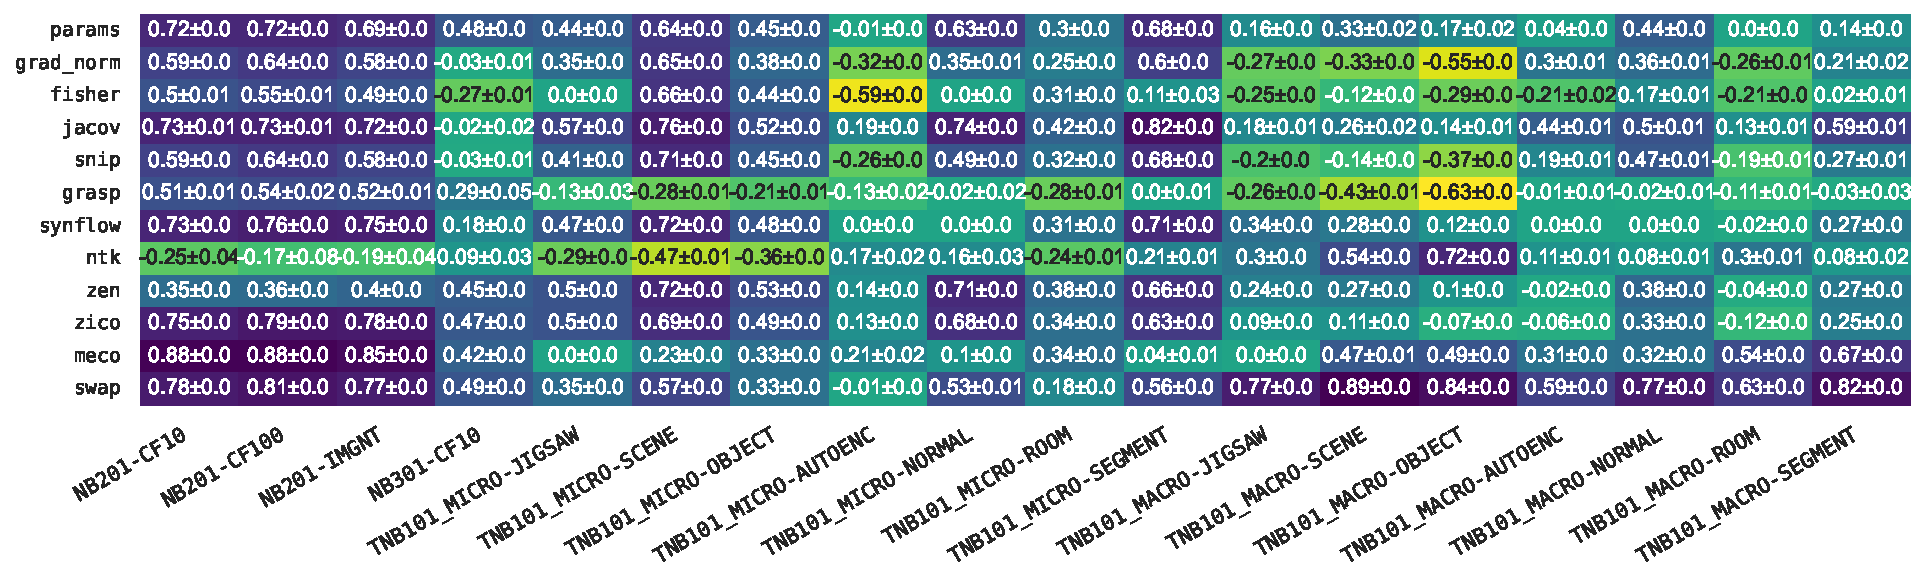
\includegraphics[width=\textwidth]{fig/benchmarks/zcp_corr_std.pdf}
\end{adjustbox}
\caption{\centering Spearman rank correlations of various ZCPs on the NAS-Bench-201, NAS-Bench-301 and TransNAS-Bench-101 benchmarks. Spearman was computed over 3 seeds against the entire search space.}
\label{fig_bench_corr_full_std}
\end{figure}

\begin{figure}[H]
\begin{adjustbox}{width=\linewidth}
    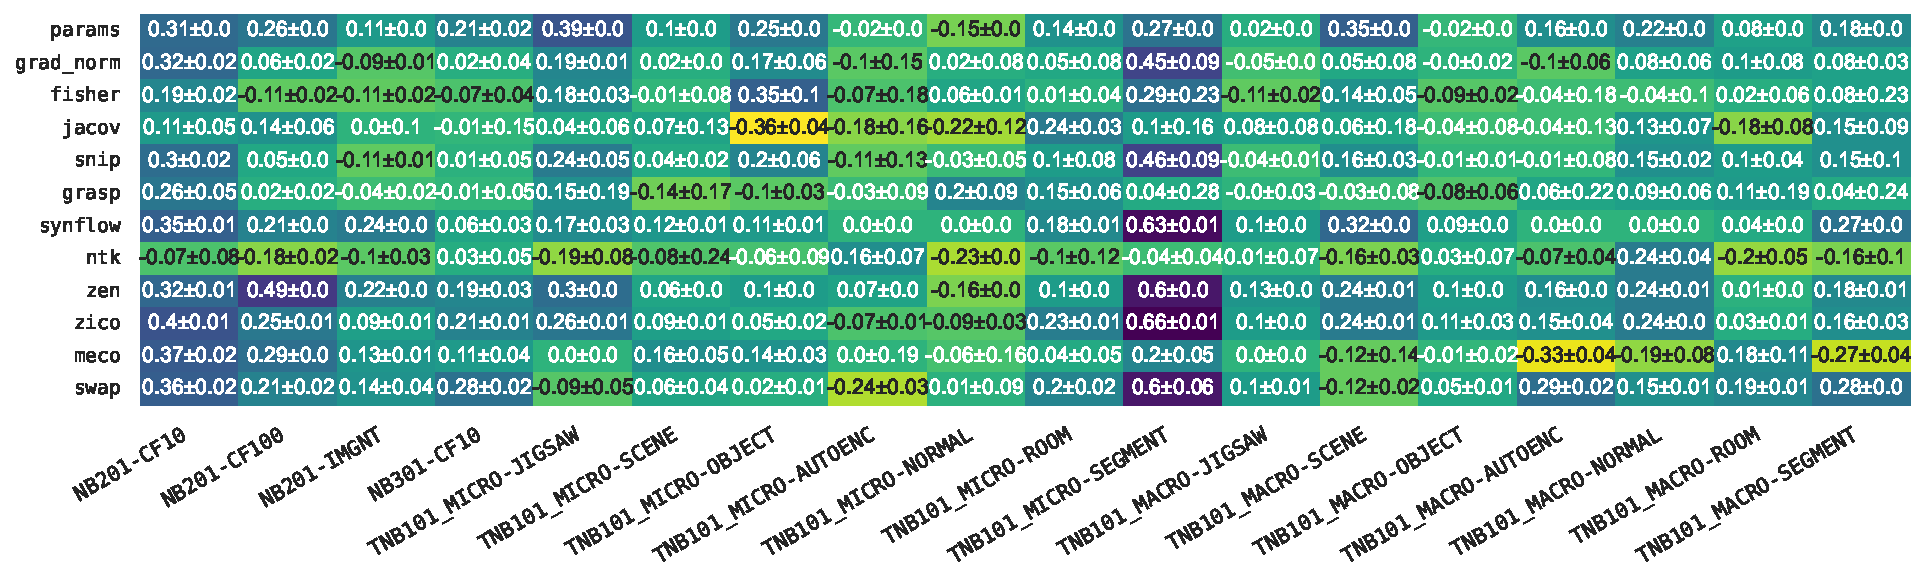
\includegraphics[width=\textwidth]{fig/benchmarks/zcp_corr_top1pct_std.pdf}
\end{adjustbox}
\caption{\centering Spearman rank correlations of various ZCPs on the NB201, NB301 and TNB101 benchmarks. Spearman was computed on 3 seeds against the top 1\% architectures in the space.}
\label{fig_bench_corr_top_std}
\end{figure}

\end{document}